\chapter{Methods}
\label{chap:concept}

In this chapter, the methods proposed in this thesis are derived and presented on an example to build up intuition. The methods are:
\begin{itemize}
    \item \textbf{\gls{uitvbo}:} A modeling approach to \gls{tvbo} incorporating \gls{ui} forgetting.
    \item \textbf{\gls{ctvbo}:} An method embedding prior knowledge about the shape of the objective function into \gls{tvbo} using shape constraints.
\end{itemize}
Afterwards, extensions which are relevant for the practical application of both methods are discussed.

\section{Uncertainty-Injection Forgetting in Time-Varying Bayesian Optimization}
\label{sec:forgetting_strategies}

The current state-of-the-art modeling for forgetting in \gls{tvbo} is B2P forgetting. According to Definition \ref{def:b2p}, the expectation about a function value propagates back to the prior belief over time, losing all information. Meanwhile, \gls{ui} forgetting is expressed by increasing the variance over time and, the key difference compared to \gls{b2p} forgetting, maintaining structural information of the function value in the form of the posterior mean. Therefore, inspired by \textcite{Slivkins_2008}, the modeling approach \gls{uitvbo} is introduced and transfers the concept of \gls{ui} forgetting to the infinite bandit setting in \gls{tvbo} to retain structural information.

The intuition behind \gls{ui} forgetting is gradual change. Figure~\ref{fig:intuition_ui} shows an example with measurements taken at a fixed spatial coordinate $x_1$ of an objective function at time steps $t_1$--$t_4$. If no prior knowledge about a drift in the objective function is available, the expected value remains constant until the next measurement. However, the variance increases due to the exact value becoming more uncertain over time. As in \textcite{Slivkins_2008}, this can be formalized as a Wiener process.
\begin{figure}[t]
    \centering
    %% Creator: Matplotlib, PGF backend
%%
%% To include the figure in your LaTeX document, write
%%   \input{<filename>.pgf}
%%
%% Make sure the required packages are loaded in your preamble
%%   \usepackage{pgf}
%%
%% Figures using additional raster images can only be included by \input if
%% they are in the same directory as the main LaTeX file. For loading figures
%% from other directories you can use the `import` package
%%   \usepackage{import}
%%
%% and then include the figures with
%%   \import{<path to file>}{<filename>.pgf}
%%
%% Matplotlib used the following preamble
%%   \usepackage[utf8x]{inputenc}\usepackage[light]{kpfonts}\usepackage{amsfonts}
%%   \usepackage{fontspec}
%%
\begingroup%
\makeatletter%
\begin{pgfpicture}%
\pgfpathrectangle{\pgfpointorigin}{\pgfqpoint{5.507126in}{2.212334in}}%
\pgfusepath{use as bounding box, clip}%
\begin{pgfscope}%
\pgfsetbuttcap%
\pgfsetmiterjoin%
\definecolor{currentfill}{rgb}{1.000000,1.000000,1.000000}%
\pgfsetfillcolor{currentfill}%
\pgfsetlinewidth{0.000000pt}%
\definecolor{currentstroke}{rgb}{1.000000,1.000000,1.000000}%
\pgfsetstrokecolor{currentstroke}%
\pgfsetdash{}{0pt}%
\pgfpathmoveto{\pgfqpoint{0.000000in}{0.000000in}}%
\pgfpathlineto{\pgfqpoint{5.507126in}{0.000000in}}%
\pgfpathlineto{\pgfqpoint{5.507126in}{2.212334in}}%
\pgfpathlineto{\pgfqpoint{0.000000in}{2.212334in}}%
\pgfpathclose%
\pgfusepath{fill}%
\end{pgfscope}%
\begin{pgfscope}%
\pgfsetbuttcap%
\pgfsetmiterjoin%
\definecolor{currentfill}{rgb}{1.000000,1.000000,1.000000}%
\pgfsetfillcolor{currentfill}%
\pgfsetlinewidth{0.000000pt}%
\definecolor{currentstroke}{rgb}{0.000000,0.000000,0.000000}%
\pgfsetstrokecolor{currentstroke}%
\pgfsetstrokeopacity{0.000000}%
\pgfsetdash{}{0pt}%
\pgfpathmoveto{\pgfqpoint{0.275356in}{0.287603in}}%
\pgfpathlineto{\pgfqpoint{2.773711in}{0.287603in}}%
\pgfpathlineto{\pgfqpoint{2.773711in}{2.101717in}}%
\pgfpathlineto{\pgfqpoint{0.275356in}{2.101717in}}%
\pgfpathclose%
\pgfusepath{fill}%
\end{pgfscope}%
\begin{pgfscope}%
\pgfpathrectangle{\pgfqpoint{0.275356in}{0.287603in}}{\pgfqpoint{2.498355in}{1.814114in}}%
\pgfusepath{clip}%
\pgfsetbuttcap%
\pgfsetroundjoin%
\definecolor{currentfill}{rgb}{0.611765,0.619608,0.623529}%
\pgfsetfillcolor{currentfill}%
\pgfsetfillopacity{0.700000}%
\pgfsetlinewidth{0.000000pt}%
\definecolor{currentstroke}{rgb}{0.611765,0.619608,0.623529}%
\pgfsetstrokecolor{currentstroke}%
\pgfsetstrokeopacity{0.700000}%
\pgfsetdash{}{0pt}%
\pgfsys@defobject{currentmarker}{\pgfqpoint{0.431503in}{0.332764in}}{\pgfqpoint{0.743798in}{1.279079in}}{%
\pgfpathmoveto{\pgfqpoint{0.431503in}{0.805922in}}%
\pgfpathlineto{\pgfqpoint{0.431503in}{0.805922in}}%
\pgfpathlineto{\pgfqpoint{0.447940in}{0.697372in}}%
\pgfpathlineto{\pgfqpoint{0.464377in}{0.652409in}}%
\pgfpathlineto{\pgfqpoint{0.480813in}{0.617908in}}%
\pgfpathlineto{\pgfqpoint{0.497250in}{0.588822in}}%
\pgfpathlineto{\pgfqpoint{0.513686in}{0.563197in}}%
\pgfpathlineto{\pgfqpoint{0.530123in}{0.540030in}}%
\pgfpathlineto{\pgfqpoint{0.546559in}{0.518726in}}%
\pgfpathlineto{\pgfqpoint{0.562996in}{0.498896in}}%
\pgfpathlineto{\pgfqpoint{0.579432in}{0.480272in}}%
\pgfpathlineto{\pgfqpoint{0.595869in}{0.462657in}}%
\pgfpathlineto{\pgfqpoint{0.612305in}{0.445903in}}%
\pgfpathlineto{\pgfqpoint{0.628742in}{0.429894in}}%
\pgfpathlineto{\pgfqpoint{0.645179in}{0.414540in}}%
\pgfpathlineto{\pgfqpoint{0.661615in}{0.399765in}}%
\pgfpathlineto{\pgfqpoint{0.678052in}{0.385510in}}%
\pgfpathlineto{\pgfqpoint{0.694488in}{0.371722in}}%
\pgfpathlineto{\pgfqpoint{0.710925in}{0.358359in}}%
\pgfpathlineto{\pgfqpoint{0.727361in}{0.345384in}}%
\pgfpathlineto{\pgfqpoint{0.743798in}{0.332764in}}%
\pgfpathlineto{\pgfqpoint{0.743798in}{1.279079in}}%
\pgfpathlineto{\pgfqpoint{0.743798in}{1.279079in}}%
\pgfpathlineto{\pgfqpoint{0.727361in}{1.266460in}}%
\pgfpathlineto{\pgfqpoint{0.710925in}{1.253484in}}%
\pgfpathlineto{\pgfqpoint{0.694488in}{1.240121in}}%
\pgfpathlineto{\pgfqpoint{0.678052in}{1.226333in}}%
\pgfpathlineto{\pgfqpoint{0.661615in}{1.212078in}}%
\pgfpathlineto{\pgfqpoint{0.645179in}{1.197304in}}%
\pgfpathlineto{\pgfqpoint{0.628742in}{1.181949in}}%
\pgfpathlineto{\pgfqpoint{0.612305in}{1.165941in}}%
\pgfpathlineto{\pgfqpoint{0.595869in}{1.149186in}}%
\pgfpathlineto{\pgfqpoint{0.579432in}{1.131571in}}%
\pgfpathlineto{\pgfqpoint{0.562996in}{1.112947in}}%
\pgfpathlineto{\pgfqpoint{0.546559in}{1.093118in}}%
\pgfpathlineto{\pgfqpoint{0.530123in}{1.071813in}}%
\pgfpathlineto{\pgfqpoint{0.513686in}{1.048647in}}%
\pgfpathlineto{\pgfqpoint{0.497250in}{1.023021in}}%
\pgfpathlineto{\pgfqpoint{0.480813in}{0.993936in}}%
\pgfpathlineto{\pgfqpoint{0.464377in}{0.959434in}}%
\pgfpathlineto{\pgfqpoint{0.447940in}{0.914472in}}%
\pgfpathlineto{\pgfqpoint{0.431503in}{0.805922in}}%
\pgfpathclose%
\pgfusepath{fill}%
}%
\begin{pgfscope}%
\pgfsys@transformshift{0.000000in}{0.000000in}%
\pgfsys@useobject{currentmarker}{}%
\end{pgfscope}%
\end{pgfscope}%
\begin{pgfscope}%
\pgfpathrectangle{\pgfqpoint{0.275356in}{0.287603in}}{\pgfqpoint{2.498355in}{1.814114in}}%
\pgfusepath{clip}%
\pgfsetbuttcap%
\pgfsetroundjoin%
\definecolor{currentfill}{rgb}{0.611765,0.619608,0.623529}%
\pgfsetfillcolor{currentfill}%
\pgfsetfillopacity{0.700000}%
\pgfsetlinewidth{0.000000pt}%
\definecolor{currentstroke}{rgb}{0.611765,0.619608,0.623529}%
\pgfsetstrokecolor{currentstroke}%
\pgfsetstrokeopacity{0.700000}%
\pgfsetdash{}{0pt}%
\pgfsys@defobject{currentmarker}{\pgfqpoint{0.743798in}{0.656713in}}{\pgfqpoint{1.056092in}{1.603028in}}{%
\pgfpathmoveto{\pgfqpoint{0.743798in}{1.129871in}}%
\pgfpathlineto{\pgfqpoint{0.743798in}{1.129871in}}%
\pgfpathlineto{\pgfqpoint{0.760234in}{1.021321in}}%
\pgfpathlineto{\pgfqpoint{0.776671in}{0.976358in}}%
\pgfpathlineto{\pgfqpoint{0.793107in}{0.941857in}}%
\pgfpathlineto{\pgfqpoint{0.809544in}{0.912771in}}%
\pgfpathlineto{\pgfqpoint{0.825981in}{0.887146in}}%
\pgfpathlineto{\pgfqpoint{0.842417in}{0.863979in}}%
\pgfpathlineto{\pgfqpoint{0.858854in}{0.842675in}}%
\pgfpathlineto{\pgfqpoint{0.875290in}{0.822845in}}%
\pgfpathlineto{\pgfqpoint{0.891727in}{0.804221in}}%
\pgfpathlineto{\pgfqpoint{0.908163in}{0.786606in}}%
\pgfpathlineto{\pgfqpoint{0.924600in}{0.769852in}}%
\pgfpathlineto{\pgfqpoint{0.941036in}{0.753843in}}%
\pgfpathlineto{\pgfqpoint{0.957473in}{0.738489in}}%
\pgfpathlineto{\pgfqpoint{0.973909in}{0.723714in}}%
\pgfpathlineto{\pgfqpoint{0.990346in}{0.709459in}}%
\pgfpathlineto{\pgfqpoint{1.006783in}{0.695671in}}%
\pgfpathlineto{\pgfqpoint{1.023219in}{0.682308in}}%
\pgfpathlineto{\pgfqpoint{1.039656in}{0.669333in}}%
\pgfpathlineto{\pgfqpoint{1.056092in}{0.656713in}}%
\pgfpathlineto{\pgfqpoint{1.056092in}{1.603028in}}%
\pgfpathlineto{\pgfqpoint{1.056092in}{1.603028in}}%
\pgfpathlineto{\pgfqpoint{1.039656in}{1.590409in}}%
\pgfpathlineto{\pgfqpoint{1.023219in}{1.577433in}}%
\pgfpathlineto{\pgfqpoint{1.006783in}{1.564070in}}%
\pgfpathlineto{\pgfqpoint{0.990346in}{1.550282in}}%
\pgfpathlineto{\pgfqpoint{0.973909in}{1.536027in}}%
\pgfpathlineto{\pgfqpoint{0.957473in}{1.521253in}}%
\pgfpathlineto{\pgfqpoint{0.941036in}{1.505898in}}%
\pgfpathlineto{\pgfqpoint{0.924600in}{1.489890in}}%
\pgfpathlineto{\pgfqpoint{0.908163in}{1.473135in}}%
\pgfpathlineto{\pgfqpoint{0.891727in}{1.455520in}}%
\pgfpathlineto{\pgfqpoint{0.875290in}{1.436896in}}%
\pgfpathlineto{\pgfqpoint{0.858854in}{1.417067in}}%
\pgfpathlineto{\pgfqpoint{0.842417in}{1.395762in}}%
\pgfpathlineto{\pgfqpoint{0.825981in}{1.372595in}}%
\pgfpathlineto{\pgfqpoint{0.809544in}{1.346970in}}%
\pgfpathlineto{\pgfqpoint{0.793107in}{1.317884in}}%
\pgfpathlineto{\pgfqpoint{0.776671in}{1.283383in}}%
\pgfpathlineto{\pgfqpoint{0.760234in}{1.238421in}}%
\pgfpathlineto{\pgfqpoint{0.743798in}{1.129871in}}%
\pgfpathclose%
\pgfusepath{fill}%
}%
\begin{pgfscope}%
\pgfsys@transformshift{0.000000in}{0.000000in}%
\pgfsys@useobject{currentmarker}{}%
\end{pgfscope}%
\end{pgfscope}%
\begin{pgfscope}%
\pgfpathrectangle{\pgfqpoint{0.275356in}{0.287603in}}{\pgfqpoint{2.498355in}{1.814114in}}%
\pgfusepath{clip}%
\pgfsetbuttcap%
\pgfsetroundjoin%
\definecolor{currentfill}{rgb}{0.611765,0.619608,0.623529}%
\pgfsetfillcolor{currentfill}%
\pgfsetfillopacity{0.700000}%
\pgfsetlinewidth{0.000000pt}%
\definecolor{currentstroke}{rgb}{0.611765,0.619608,0.623529}%
\pgfsetstrokecolor{currentstroke}%
\pgfsetstrokeopacity{0.700000}%
\pgfsetdash{}{0pt}%
\pgfsys@defobject{currentmarker}{\pgfqpoint{1.056092in}{0.442390in}}{\pgfqpoint{1.524534in}{1.601385in}}{%
\pgfpathmoveto{\pgfqpoint{1.056092in}{1.021888in}}%
\pgfpathlineto{\pgfqpoint{1.056092in}{1.021888in}}%
\pgfpathlineto{\pgfqpoint{1.080747in}{0.888942in}}%
\pgfpathlineto{\pgfqpoint{1.105402in}{0.833874in}}%
\pgfpathlineto{\pgfqpoint{1.130057in}{0.791619in}}%
\pgfpathlineto{\pgfqpoint{1.154711in}{0.755996in}}%
\pgfpathlineto{\pgfqpoint{1.179366in}{0.724612in}}%
\pgfpathlineto{\pgfqpoint{1.204021in}{0.696238in}}%
\pgfpathlineto{\pgfqpoint{1.228676in}{0.670146in}}%
\pgfpathlineto{\pgfqpoint{1.253331in}{0.645860in}}%
\pgfpathlineto{\pgfqpoint{1.277986in}{0.623050in}}%
\pgfpathlineto{\pgfqpoint{1.302640in}{0.601476in}}%
\pgfpathlineto{\pgfqpoint{1.327295in}{0.580956in}}%
\pgfpathlineto{\pgfqpoint{1.351950in}{0.561350in}}%
\pgfpathlineto{\pgfqpoint{1.376605in}{0.542545in}}%
\pgfpathlineto{\pgfqpoint{1.401260in}{0.524450in}}%
\pgfpathlineto{\pgfqpoint{1.425914in}{0.506991in}}%
\pgfpathlineto{\pgfqpoint{1.450569in}{0.490104in}}%
\pgfpathlineto{\pgfqpoint{1.475224in}{0.473738in}}%
\pgfpathlineto{\pgfqpoint{1.499879in}{0.457846in}}%
\pgfpathlineto{\pgfqpoint{1.524534in}{0.442390in}}%
\pgfpathlineto{\pgfqpoint{1.524534in}{1.601385in}}%
\pgfpathlineto{\pgfqpoint{1.524534in}{1.601385in}}%
\pgfpathlineto{\pgfqpoint{1.499879in}{1.585929in}}%
\pgfpathlineto{\pgfqpoint{1.475224in}{1.570037in}}%
\pgfpathlineto{\pgfqpoint{1.450569in}{1.553671in}}%
\pgfpathlineto{\pgfqpoint{1.425914in}{1.536785in}}%
\pgfpathlineto{\pgfqpoint{1.401260in}{1.519325in}}%
\pgfpathlineto{\pgfqpoint{1.376605in}{1.501231in}}%
\pgfpathlineto{\pgfqpoint{1.351950in}{1.482426in}}%
\pgfpathlineto{\pgfqpoint{1.327295in}{1.462819in}}%
\pgfpathlineto{\pgfqpoint{1.302640in}{1.442299in}}%
\pgfpathlineto{\pgfqpoint{1.277986in}{1.420725in}}%
\pgfpathlineto{\pgfqpoint{1.253331in}{1.397915in}}%
\pgfpathlineto{\pgfqpoint{1.228676in}{1.373629in}}%
\pgfpathlineto{\pgfqpoint{1.204021in}{1.347537in}}%
\pgfpathlineto{\pgfqpoint{1.179366in}{1.319164in}}%
\pgfpathlineto{\pgfqpoint{1.154711in}{1.287779in}}%
\pgfpathlineto{\pgfqpoint{1.130057in}{1.252157in}}%
\pgfpathlineto{\pgfqpoint{1.105402in}{1.209902in}}%
\pgfpathlineto{\pgfqpoint{1.080747in}{1.154834in}}%
\pgfpathlineto{\pgfqpoint{1.056092in}{1.021888in}}%
\pgfpathclose%
\pgfusepath{fill}%
}%
\begin{pgfscope}%
\pgfsys@transformshift{0.000000in}{0.000000in}%
\pgfsys@useobject{currentmarker}{}%
\end{pgfscope}%
\end{pgfscope}%
\begin{pgfscope}%
\pgfpathrectangle{\pgfqpoint{0.275356in}{0.287603in}}{\pgfqpoint{2.498355in}{1.814114in}}%
\pgfusepath{clip}%
\pgfsetbuttcap%
\pgfsetroundjoin%
\definecolor{currentfill}{rgb}{0.611765,0.619608,0.623529}%
\pgfsetfillcolor{currentfill}%
\pgfsetfillopacity{0.700000}%
\pgfsetlinewidth{0.000000pt}%
\definecolor{currentstroke}{rgb}{0.611765,0.619608,0.623529}%
\pgfsetstrokecolor{currentstroke}%
\pgfsetstrokeopacity{0.700000}%
\pgfsetdash{}{0pt}%
\pgfsys@defobject{currentmarker}{\pgfqpoint{1.524534in}{0.399521in}}{\pgfqpoint{2.773711in}{2.292152in}}{%
\pgfpathmoveto{\pgfqpoint{1.524534in}{1.345837in}}%
\pgfpathlineto{\pgfqpoint{1.524534in}{1.345837in}}%
\pgfpathlineto{\pgfqpoint{1.590280in}{1.128737in}}%
\pgfpathlineto{\pgfqpoint{1.656026in}{1.038811in}}%
\pgfpathlineto{\pgfqpoint{1.721772in}{0.969809in}}%
\pgfpathlineto{\pgfqpoint{1.787518in}{0.911637in}}%
\pgfpathlineto{\pgfqpoint{1.853265in}{0.860387in}}%
\pgfpathlineto{\pgfqpoint{1.919011in}{0.814053in}}%
\pgfpathlineto{\pgfqpoint{1.984757in}{0.771445in}}%
\pgfpathlineto{\pgfqpoint{2.050503in}{0.731786in}}%
\pgfpathlineto{\pgfqpoint{2.116249in}{0.694538in}}%
\pgfpathlineto{\pgfqpoint{2.181995in}{0.659307in}}%
\pgfpathlineto{\pgfqpoint{2.247742in}{0.625799in}}%
\pgfpathlineto{\pgfqpoint{2.313488in}{0.593781in}}%
\pgfpathlineto{\pgfqpoint{2.379234in}{0.563073in}}%
\pgfpathlineto{\pgfqpoint{2.444980in}{0.533524in}}%
\pgfpathlineto{\pgfqpoint{2.510726in}{0.505013in}}%
\pgfpathlineto{\pgfqpoint{2.576473in}{0.477438in}}%
\pgfpathlineto{\pgfqpoint{2.642219in}{0.450712in}}%
\pgfpathlineto{\pgfqpoint{2.707965in}{0.424761in}}%
\pgfpathlineto{\pgfqpoint{2.773711in}{0.399521in}}%
\pgfpathlineto{\pgfqpoint{2.773711in}{2.292152in}}%
\pgfpathlineto{\pgfqpoint{2.773711in}{2.292152in}}%
\pgfpathlineto{\pgfqpoint{2.707965in}{2.266912in}}%
\pgfpathlineto{\pgfqpoint{2.642219in}{2.240961in}}%
\pgfpathlineto{\pgfqpoint{2.576473in}{2.214235in}}%
\pgfpathlineto{\pgfqpoint{2.510726in}{2.186660in}}%
\pgfpathlineto{\pgfqpoint{2.444980in}{2.158149in}}%
\pgfpathlineto{\pgfqpoint{2.379234in}{2.128601in}}%
\pgfpathlineto{\pgfqpoint{2.313488in}{2.097892in}}%
\pgfpathlineto{\pgfqpoint{2.247742in}{2.065875in}}%
\pgfpathlineto{\pgfqpoint{2.181995in}{2.032366in}}%
\pgfpathlineto{\pgfqpoint{2.116249in}{1.997136in}}%
\pgfpathlineto{\pgfqpoint{2.050503in}{1.959887in}}%
\pgfpathlineto{\pgfqpoint{1.984757in}{1.920228in}}%
\pgfpathlineto{\pgfqpoint{1.919011in}{1.877620in}}%
\pgfpathlineto{\pgfqpoint{1.853265in}{1.831286in}}%
\pgfpathlineto{\pgfqpoint{1.787518in}{1.780036in}}%
\pgfpathlineto{\pgfqpoint{1.721772in}{1.721864in}}%
\pgfpathlineto{\pgfqpoint{1.656026in}{1.652862in}}%
\pgfpathlineto{\pgfqpoint{1.590280in}{1.562936in}}%
\pgfpathlineto{\pgfqpoint{1.524534in}{1.345837in}}%
\pgfpathclose%
\pgfusepath{fill}%
}%
\begin{pgfscope}%
\pgfsys@transformshift{0.000000in}{0.000000in}%
\pgfsys@useobject{currentmarker}{}%
\end{pgfscope}%
\end{pgfscope}%
\begin{pgfscope}%
\pgfsetbuttcap%
\pgfsetroundjoin%
\definecolor{currentfill}{rgb}{0.000000,0.000000,0.000000}%
\pgfsetfillcolor{currentfill}%
\pgfsetlinewidth{0.803000pt}%
\definecolor{currentstroke}{rgb}{0.000000,0.000000,0.000000}%
\pgfsetstrokecolor{currentstroke}%
\pgfsetdash{}{0pt}%
\pgfsys@defobject{currentmarker}{\pgfqpoint{0.000000in}{-0.048611in}}{\pgfqpoint{0.000000in}{0.000000in}}{%
\pgfpathmoveto{\pgfqpoint{0.000000in}{0.000000in}}%
\pgfpathlineto{\pgfqpoint{0.000000in}{-0.048611in}}%
\pgfusepath{stroke,fill}%
}%
\begin{pgfscope}%
\pgfsys@transformshift{0.431503in}{0.287603in}%
\pgfsys@useobject{currentmarker}{}%
\end{pgfscope}%
\end{pgfscope}%
\begin{pgfscope}%
\definecolor{textcolor}{rgb}{0.000000,0.000000,0.000000}%
\pgfsetstrokecolor{textcolor}%
\pgfsetfillcolor{textcolor}%
\pgftext[x=0.431503in,y=0.190381in,,top]{\color{textcolor}\rmfamily\fontsize{10.000000}{12.000000}\selectfont \(\displaystyle t_1\)}%
\end{pgfscope}%
\begin{pgfscope}%
\pgfsetbuttcap%
\pgfsetroundjoin%
\definecolor{currentfill}{rgb}{0.000000,0.000000,0.000000}%
\pgfsetfillcolor{currentfill}%
\pgfsetlinewidth{0.803000pt}%
\definecolor{currentstroke}{rgb}{0.000000,0.000000,0.000000}%
\pgfsetstrokecolor{currentstroke}%
\pgfsetdash{}{0pt}%
\pgfsys@defobject{currentmarker}{\pgfqpoint{0.000000in}{-0.048611in}}{\pgfqpoint{0.000000in}{0.000000in}}{%
\pgfpathmoveto{\pgfqpoint{0.000000in}{0.000000in}}%
\pgfpathlineto{\pgfqpoint{0.000000in}{-0.048611in}}%
\pgfusepath{stroke,fill}%
}%
\begin{pgfscope}%
\pgfsys@transformshift{0.743798in}{0.287603in}%
\pgfsys@useobject{currentmarker}{}%
\end{pgfscope}%
\end{pgfscope}%
\begin{pgfscope}%
\definecolor{textcolor}{rgb}{0.000000,0.000000,0.000000}%
\pgfsetstrokecolor{textcolor}%
\pgfsetfillcolor{textcolor}%
\pgftext[x=0.743798in,y=0.190381in,,top]{\color{textcolor}\rmfamily\fontsize{10.000000}{12.000000}\selectfont \(\displaystyle t_2\)}%
\end{pgfscope}%
\begin{pgfscope}%
\pgfsetbuttcap%
\pgfsetroundjoin%
\definecolor{currentfill}{rgb}{0.000000,0.000000,0.000000}%
\pgfsetfillcolor{currentfill}%
\pgfsetlinewidth{0.803000pt}%
\definecolor{currentstroke}{rgb}{0.000000,0.000000,0.000000}%
\pgfsetstrokecolor{currentstroke}%
\pgfsetdash{}{0pt}%
\pgfsys@defobject{currentmarker}{\pgfqpoint{0.000000in}{-0.048611in}}{\pgfqpoint{0.000000in}{0.000000in}}{%
\pgfpathmoveto{\pgfqpoint{0.000000in}{0.000000in}}%
\pgfpathlineto{\pgfqpoint{0.000000in}{-0.048611in}}%
\pgfusepath{stroke,fill}%
}%
\begin{pgfscope}%
\pgfsys@transformshift{1.056092in}{0.287603in}%
\pgfsys@useobject{currentmarker}{}%
\end{pgfscope}%
\end{pgfscope}%
\begin{pgfscope}%
\definecolor{textcolor}{rgb}{0.000000,0.000000,0.000000}%
\pgfsetstrokecolor{textcolor}%
\pgfsetfillcolor{textcolor}%
\pgftext[x=1.056092in,y=0.190381in,,top]{\color{textcolor}\rmfamily\fontsize{10.000000}{12.000000}\selectfont \(\displaystyle t_3\)}%
\end{pgfscope}%
\begin{pgfscope}%
\pgfsetbuttcap%
\pgfsetroundjoin%
\definecolor{currentfill}{rgb}{0.000000,0.000000,0.000000}%
\pgfsetfillcolor{currentfill}%
\pgfsetlinewidth{0.803000pt}%
\definecolor{currentstroke}{rgb}{0.000000,0.000000,0.000000}%
\pgfsetstrokecolor{currentstroke}%
\pgfsetdash{}{0pt}%
\pgfsys@defobject{currentmarker}{\pgfqpoint{0.000000in}{-0.048611in}}{\pgfqpoint{0.000000in}{0.000000in}}{%
\pgfpathmoveto{\pgfqpoint{0.000000in}{0.000000in}}%
\pgfpathlineto{\pgfqpoint{0.000000in}{-0.048611in}}%
\pgfusepath{stroke,fill}%
}%
\begin{pgfscope}%
\pgfsys@transformshift{1.524534in}{0.287603in}%
\pgfsys@useobject{currentmarker}{}%
\end{pgfscope}%
\end{pgfscope}%
\begin{pgfscope}%
\definecolor{textcolor}{rgb}{0.000000,0.000000,0.000000}%
\pgfsetstrokecolor{textcolor}%
\pgfsetfillcolor{textcolor}%
\pgftext[x=1.524534in,y=0.190381in,,top]{\color{textcolor}\rmfamily\fontsize{10.000000}{12.000000}\selectfont \(\displaystyle t_4\)}%
\end{pgfscope}%
\begin{pgfscope}%
\pgfsetbuttcap%
\pgfsetroundjoin%
\definecolor{currentfill}{rgb}{0.000000,0.000000,0.000000}%
\pgfsetfillcolor{currentfill}%
\pgfsetlinewidth{0.803000pt}%
\definecolor{currentstroke}{rgb}{0.000000,0.000000,0.000000}%
\pgfsetstrokecolor{currentstroke}%
\pgfsetdash{}{0pt}%
\pgfsys@defobject{currentmarker}{\pgfqpoint{-0.048611in}{0.000000in}}{\pgfqpoint{-0.000000in}{0.000000in}}{%
\pgfpathmoveto{\pgfqpoint{-0.000000in}{0.000000in}}%
\pgfpathlineto{\pgfqpoint{-0.048611in}{0.000000in}}%
\pgfusepath{stroke,fill}%
}%
\begin{pgfscope}%
\pgfsys@transformshift{0.275356in}{0.373990in}%
\pgfsys@useobject{currentmarker}{}%
\end{pgfscope}%
\end{pgfscope}%
\begin{pgfscope}%
\pgfsetbuttcap%
\pgfsetroundjoin%
\definecolor{currentfill}{rgb}{0.000000,0.000000,0.000000}%
\pgfsetfillcolor{currentfill}%
\pgfsetlinewidth{0.803000pt}%
\definecolor{currentstroke}{rgb}{0.000000,0.000000,0.000000}%
\pgfsetstrokecolor{currentstroke}%
\pgfsetdash{}{0pt}%
\pgfsys@defobject{currentmarker}{\pgfqpoint{-0.048611in}{0.000000in}}{\pgfqpoint{-0.000000in}{0.000000in}}{%
\pgfpathmoveto{\pgfqpoint{-0.000000in}{0.000000in}}%
\pgfpathlineto{\pgfqpoint{-0.048611in}{0.000000in}}%
\pgfusepath{stroke,fill}%
}%
\begin{pgfscope}%
\pgfsys@transformshift{0.275356in}{0.805922in}%
\pgfsys@useobject{currentmarker}{}%
\end{pgfscope}%
\end{pgfscope}%
\begin{pgfscope}%
\pgfsetbuttcap%
\pgfsetroundjoin%
\definecolor{currentfill}{rgb}{0.000000,0.000000,0.000000}%
\pgfsetfillcolor{currentfill}%
\pgfsetlinewidth{0.803000pt}%
\definecolor{currentstroke}{rgb}{0.000000,0.000000,0.000000}%
\pgfsetstrokecolor{currentstroke}%
\pgfsetdash{}{0pt}%
\pgfsys@defobject{currentmarker}{\pgfqpoint{-0.048611in}{0.000000in}}{\pgfqpoint{-0.000000in}{0.000000in}}{%
\pgfpathmoveto{\pgfqpoint{-0.000000in}{0.000000in}}%
\pgfpathlineto{\pgfqpoint{-0.048611in}{0.000000in}}%
\pgfusepath{stroke,fill}%
}%
\begin{pgfscope}%
\pgfsys@transformshift{0.275356in}{1.237854in}%
\pgfsys@useobject{currentmarker}{}%
\end{pgfscope}%
\end{pgfscope}%
\begin{pgfscope}%
\pgfsetbuttcap%
\pgfsetroundjoin%
\definecolor{currentfill}{rgb}{0.000000,0.000000,0.000000}%
\pgfsetfillcolor{currentfill}%
\pgfsetlinewidth{0.803000pt}%
\definecolor{currentstroke}{rgb}{0.000000,0.000000,0.000000}%
\pgfsetstrokecolor{currentstroke}%
\pgfsetdash{}{0pt}%
\pgfsys@defobject{currentmarker}{\pgfqpoint{-0.048611in}{0.000000in}}{\pgfqpoint{-0.000000in}{0.000000in}}{%
\pgfpathmoveto{\pgfqpoint{-0.000000in}{0.000000in}}%
\pgfpathlineto{\pgfqpoint{-0.048611in}{0.000000in}}%
\pgfusepath{stroke,fill}%
}%
\begin{pgfscope}%
\pgfsys@transformshift{0.275356in}{1.669786in}%
\pgfsys@useobject{currentmarker}{}%
\end{pgfscope}%
\end{pgfscope}%
\begin{pgfscope}%
\definecolor{textcolor}{rgb}{0.000000,0.000000,0.000000}%
\pgfsetstrokecolor{textcolor}%
\pgfsetfillcolor{textcolor}%
\pgftext[x=0.219801in,y=1.194660in,,bottom,rotate=90.000000]{\color{textcolor}\rmfamily\fontsize{10.000000}{12.000000}\selectfont \(\displaystyle f_t(x=x_1)\)}%
\end{pgfscope}%
\begin{pgfscope}%
\pgfpathrectangle{\pgfqpoint{0.275356in}{0.287603in}}{\pgfqpoint{2.498355in}{1.814114in}}%
\pgfusepath{clip}%
\pgfsetbuttcap%
\pgfsetroundjoin%
\pgfsetlinewidth{1.505625pt}%
\definecolor{currentstroke}{rgb}{0.000000,0.000000,0.000000}%
\pgfsetstrokecolor{currentstroke}%
\pgfsetdash{{1.500000pt}{2.475000pt}}{0.000000pt}%
\pgfpathmoveto{\pgfqpoint{0.275356in}{0.373990in}}%
\pgfpathlineto{\pgfqpoint{2.773711in}{0.373990in}}%
\pgfusepath{stroke}%
\end{pgfscope}%
\begin{pgfscope}%
\pgfpathrectangle{\pgfqpoint{0.275356in}{0.287603in}}{\pgfqpoint{2.498355in}{1.814114in}}%
\pgfusepath{clip}%
\pgfsetbuttcap%
\pgfsetroundjoin%
\pgfsetlinewidth{1.505625pt}%
\definecolor{currentstroke}{rgb}{0.392157,0.396078,0.403922}%
\pgfsetstrokecolor{currentstroke}%
\pgfsetdash{{5.550000pt}{2.400000pt}}{0.000000pt}%
\pgfpathmoveto{\pgfqpoint{0.431503in}{0.805922in}}%
\pgfpathlineto{\pgfqpoint{0.447940in}{0.805922in}}%
\pgfpathlineto{\pgfqpoint{0.464377in}{0.805922in}}%
\pgfpathlineto{\pgfqpoint{0.480813in}{0.805922in}}%
\pgfpathlineto{\pgfqpoint{0.497250in}{0.805922in}}%
\pgfpathlineto{\pgfqpoint{0.513686in}{0.805922in}}%
\pgfpathlineto{\pgfqpoint{0.530123in}{0.805922in}}%
\pgfpathlineto{\pgfqpoint{0.546559in}{0.805922in}}%
\pgfpathlineto{\pgfqpoint{0.562996in}{0.805922in}}%
\pgfpathlineto{\pgfqpoint{0.579432in}{0.805922in}}%
\pgfpathlineto{\pgfqpoint{0.595869in}{0.805922in}}%
\pgfpathlineto{\pgfqpoint{0.612305in}{0.805922in}}%
\pgfpathlineto{\pgfqpoint{0.628742in}{0.805922in}}%
\pgfpathlineto{\pgfqpoint{0.645179in}{0.805922in}}%
\pgfpathlineto{\pgfqpoint{0.661615in}{0.805922in}}%
\pgfpathlineto{\pgfqpoint{0.678052in}{0.805922in}}%
\pgfpathlineto{\pgfqpoint{0.694488in}{0.805922in}}%
\pgfpathlineto{\pgfqpoint{0.710925in}{0.805922in}}%
\pgfpathlineto{\pgfqpoint{0.727361in}{0.805922in}}%
\pgfpathlineto{\pgfqpoint{0.743798in}{0.805922in}}%
\pgfusepath{stroke}%
\end{pgfscope}%
\begin{pgfscope}%
\pgfpathrectangle{\pgfqpoint{0.275356in}{0.287603in}}{\pgfqpoint{2.498355in}{1.814114in}}%
\pgfusepath{clip}%
\pgfsetbuttcap%
\pgfsetroundjoin%
\pgfsetlinewidth{1.505625pt}%
\definecolor{currentstroke}{rgb}{0.392157,0.396078,0.403922}%
\pgfsetstrokecolor{currentstroke}%
\pgfsetdash{{5.550000pt}{2.400000pt}}{0.000000pt}%
\pgfpathmoveto{\pgfqpoint{0.743798in}{1.129871in}}%
\pgfpathlineto{\pgfqpoint{0.760234in}{1.129871in}}%
\pgfpathlineto{\pgfqpoint{0.776671in}{1.129871in}}%
\pgfpathlineto{\pgfqpoint{0.793107in}{1.129871in}}%
\pgfpathlineto{\pgfqpoint{0.809544in}{1.129871in}}%
\pgfpathlineto{\pgfqpoint{0.825981in}{1.129871in}}%
\pgfpathlineto{\pgfqpoint{0.842417in}{1.129871in}}%
\pgfpathlineto{\pgfqpoint{0.858854in}{1.129871in}}%
\pgfpathlineto{\pgfqpoint{0.875290in}{1.129871in}}%
\pgfpathlineto{\pgfqpoint{0.891727in}{1.129871in}}%
\pgfpathlineto{\pgfqpoint{0.908163in}{1.129871in}}%
\pgfpathlineto{\pgfqpoint{0.924600in}{1.129871in}}%
\pgfpathlineto{\pgfqpoint{0.941036in}{1.129871in}}%
\pgfpathlineto{\pgfqpoint{0.957473in}{1.129871in}}%
\pgfpathlineto{\pgfqpoint{0.973909in}{1.129871in}}%
\pgfpathlineto{\pgfqpoint{0.990346in}{1.129871in}}%
\pgfpathlineto{\pgfqpoint{1.006783in}{1.129871in}}%
\pgfpathlineto{\pgfqpoint{1.023219in}{1.129871in}}%
\pgfpathlineto{\pgfqpoint{1.039656in}{1.129871in}}%
\pgfpathlineto{\pgfqpoint{1.056092in}{1.129871in}}%
\pgfusepath{stroke}%
\end{pgfscope}%
\begin{pgfscope}%
\pgfpathrectangle{\pgfqpoint{0.275356in}{0.287603in}}{\pgfqpoint{2.498355in}{1.814114in}}%
\pgfusepath{clip}%
\pgfsetbuttcap%
\pgfsetroundjoin%
\pgfsetlinewidth{1.505625pt}%
\definecolor{currentstroke}{rgb}{0.392157,0.396078,0.403922}%
\pgfsetstrokecolor{currentstroke}%
\pgfsetdash{{5.550000pt}{2.400000pt}}{0.000000pt}%
\pgfpathmoveto{\pgfqpoint{1.056092in}{1.021888in}}%
\pgfpathlineto{\pgfqpoint{1.080747in}{1.021888in}}%
\pgfpathlineto{\pgfqpoint{1.105402in}{1.021888in}}%
\pgfpathlineto{\pgfqpoint{1.130057in}{1.021888in}}%
\pgfpathlineto{\pgfqpoint{1.154711in}{1.021888in}}%
\pgfpathlineto{\pgfqpoint{1.179366in}{1.021888in}}%
\pgfpathlineto{\pgfqpoint{1.204021in}{1.021888in}}%
\pgfpathlineto{\pgfqpoint{1.228676in}{1.021888in}}%
\pgfpathlineto{\pgfqpoint{1.253331in}{1.021888in}}%
\pgfpathlineto{\pgfqpoint{1.277986in}{1.021888in}}%
\pgfpathlineto{\pgfqpoint{1.302640in}{1.021888in}}%
\pgfpathlineto{\pgfqpoint{1.327295in}{1.021888in}}%
\pgfpathlineto{\pgfqpoint{1.351950in}{1.021888in}}%
\pgfpathlineto{\pgfqpoint{1.376605in}{1.021888in}}%
\pgfpathlineto{\pgfqpoint{1.401260in}{1.021888in}}%
\pgfpathlineto{\pgfqpoint{1.425914in}{1.021888in}}%
\pgfpathlineto{\pgfqpoint{1.450569in}{1.021888in}}%
\pgfpathlineto{\pgfqpoint{1.475224in}{1.021888in}}%
\pgfpathlineto{\pgfqpoint{1.499879in}{1.021888in}}%
\pgfpathlineto{\pgfqpoint{1.524534in}{1.021888in}}%
\pgfusepath{stroke}%
\end{pgfscope}%
\begin{pgfscope}%
\pgfpathrectangle{\pgfqpoint{0.275356in}{0.287603in}}{\pgfqpoint{2.498355in}{1.814114in}}%
\pgfusepath{clip}%
\pgfsetbuttcap%
\pgfsetroundjoin%
\pgfsetlinewidth{1.505625pt}%
\definecolor{currentstroke}{rgb}{0.392157,0.396078,0.403922}%
\pgfsetstrokecolor{currentstroke}%
\pgfsetdash{{5.550000pt}{2.400000pt}}{0.000000pt}%
\pgfpathmoveto{\pgfqpoint{1.524534in}{1.345837in}}%
\pgfpathlineto{\pgfqpoint{1.590280in}{1.345837in}}%
\pgfpathlineto{\pgfqpoint{1.656026in}{1.345837in}}%
\pgfpathlineto{\pgfqpoint{1.721772in}{1.345837in}}%
\pgfpathlineto{\pgfqpoint{1.787518in}{1.345837in}}%
\pgfpathlineto{\pgfqpoint{1.853265in}{1.345837in}}%
\pgfpathlineto{\pgfqpoint{1.919011in}{1.345837in}}%
\pgfpathlineto{\pgfqpoint{1.984757in}{1.345837in}}%
\pgfpathlineto{\pgfqpoint{2.050503in}{1.345837in}}%
\pgfpathlineto{\pgfqpoint{2.116249in}{1.345837in}}%
\pgfpathlineto{\pgfqpoint{2.181995in}{1.345837in}}%
\pgfpathlineto{\pgfqpoint{2.247742in}{1.345837in}}%
\pgfpathlineto{\pgfqpoint{2.313488in}{1.345837in}}%
\pgfpathlineto{\pgfqpoint{2.379234in}{1.345837in}}%
\pgfpathlineto{\pgfqpoint{2.444980in}{1.345837in}}%
\pgfpathlineto{\pgfqpoint{2.510726in}{1.345837in}}%
\pgfpathlineto{\pgfqpoint{2.576473in}{1.345837in}}%
\pgfpathlineto{\pgfqpoint{2.642219in}{1.345837in}}%
\pgfpathlineto{\pgfqpoint{2.707965in}{1.345837in}}%
\pgfpathlineto{\pgfqpoint{2.773711in}{1.345837in}}%
\pgfusepath{stroke}%
\end{pgfscope}%
\begin{pgfscope}%
\pgfpathrectangle{\pgfqpoint{0.275356in}{0.287603in}}{\pgfqpoint{2.498355in}{1.814114in}}%
\pgfusepath{clip}%
\pgfsetbuttcap%
\pgfsetroundjoin%
\definecolor{currentfill}{rgb}{0.000000,0.000000,0.000000}%
\pgfsetfillcolor{currentfill}%
\pgfsetlinewidth{1.003750pt}%
\definecolor{currentstroke}{rgb}{0.000000,0.000000,0.000000}%
\pgfsetstrokecolor{currentstroke}%
\pgfsetdash{}{0pt}%
\pgfsys@defobject{currentmarker}{\pgfqpoint{-0.027778in}{-0.027778in}}{\pgfqpoint{0.027778in}{0.027778in}}{%
\pgfpathmoveto{\pgfqpoint{0.000000in}{-0.027778in}}%
\pgfpathcurveto{\pgfqpoint{0.007367in}{-0.027778in}}{\pgfqpoint{0.014433in}{-0.024851in}}{\pgfqpoint{0.019642in}{-0.019642in}}%
\pgfpathcurveto{\pgfqpoint{0.024851in}{-0.014433in}}{\pgfqpoint{0.027778in}{-0.007367in}}{\pgfqpoint{0.027778in}{0.000000in}}%
\pgfpathcurveto{\pgfqpoint{0.027778in}{0.007367in}}{\pgfqpoint{0.024851in}{0.014433in}}{\pgfqpoint{0.019642in}{0.019642in}}%
\pgfpathcurveto{\pgfqpoint{0.014433in}{0.024851in}}{\pgfqpoint{0.007367in}{0.027778in}}{\pgfqpoint{0.000000in}{0.027778in}}%
\pgfpathcurveto{\pgfqpoint{-0.007367in}{0.027778in}}{\pgfqpoint{-0.014433in}{0.024851in}}{\pgfqpoint{-0.019642in}{0.019642in}}%
\pgfpathcurveto{\pgfqpoint{-0.024851in}{0.014433in}}{\pgfqpoint{-0.027778in}{0.007367in}}{\pgfqpoint{-0.027778in}{0.000000in}}%
\pgfpathcurveto{\pgfqpoint{-0.027778in}{-0.007367in}}{\pgfqpoint{-0.024851in}{-0.014433in}}{\pgfqpoint{-0.019642in}{-0.019642in}}%
\pgfpathcurveto{\pgfqpoint{-0.014433in}{-0.024851in}}{\pgfqpoint{-0.007367in}{-0.027778in}}{\pgfqpoint{0.000000in}{-0.027778in}}%
\pgfpathclose%
\pgfusepath{stroke,fill}%
}%
\begin{pgfscope}%
\pgfsys@transformshift{0.431503in}{0.805922in}%
\pgfsys@useobject{currentmarker}{}%
\end{pgfscope}%
\begin{pgfscope}%
\pgfsys@transformshift{0.743798in}{1.129871in}%
\pgfsys@useobject{currentmarker}{}%
\end{pgfscope}%
\begin{pgfscope}%
\pgfsys@transformshift{1.056092in}{1.021888in}%
\pgfsys@useobject{currentmarker}{}%
\end{pgfscope}%
\begin{pgfscope}%
\pgfsys@transformshift{1.524534in}{1.345837in}%
\pgfsys@useobject{currentmarker}{}%
\end{pgfscope}%
\end{pgfscope}%
\begin{pgfscope}%
\pgfsetrectcap%
\pgfsetmiterjoin%
\pgfsetlinewidth{0.752812pt}%
\definecolor{currentstroke}{rgb}{0.000000,0.000000,0.000000}%
\pgfsetstrokecolor{currentstroke}%
\pgfsetdash{}{0pt}%
\pgfpathmoveto{\pgfqpoint{0.275356in}{0.287603in}}%
\pgfpathlineto{\pgfqpoint{0.275356in}{2.101717in}}%
\pgfusepath{stroke}%
\end{pgfscope}%
\begin{pgfscope}%
\pgfsetrectcap%
\pgfsetmiterjoin%
\pgfsetlinewidth{0.752812pt}%
\definecolor{currentstroke}{rgb}{0.000000,0.000000,0.000000}%
\pgfsetstrokecolor{currentstroke}%
\pgfsetdash{}{0pt}%
\pgfpathmoveto{\pgfqpoint{2.773711in}{0.287603in}}%
\pgfpathlineto{\pgfqpoint{2.773711in}{2.101717in}}%
\pgfusepath{stroke}%
\end{pgfscope}%
\begin{pgfscope}%
\pgfsetrectcap%
\pgfsetmiterjoin%
\pgfsetlinewidth{0.752812pt}%
\definecolor{currentstroke}{rgb}{0.000000,0.000000,0.000000}%
\pgfsetstrokecolor{currentstroke}%
\pgfsetdash{}{0pt}%
\pgfpathmoveto{\pgfqpoint{0.275356in}{0.287603in}}%
\pgfpathlineto{\pgfqpoint{2.773711in}{0.287603in}}%
\pgfusepath{stroke}%
\end{pgfscope}%
\begin{pgfscope}%
\pgfsetrectcap%
\pgfsetmiterjoin%
\pgfsetlinewidth{0.752812pt}%
\definecolor{currentstroke}{rgb}{0.000000,0.000000,0.000000}%
\pgfsetstrokecolor{currentstroke}%
\pgfsetdash{}{0pt}%
\pgfpathmoveto{\pgfqpoint{0.275356in}{2.101717in}}%
\pgfpathlineto{\pgfqpoint{2.773711in}{2.101717in}}%
\pgfusepath{stroke}%
\end{pgfscope}%
\begin{pgfscope}%
\definecolor{textcolor}{rgb}{0.000000,0.000000,0.000000}%
\pgfsetstrokecolor{textcolor}%
\pgfsetfillcolor{textcolor}%
\pgftext[x=2.055434in,y=1.389030in,,bottom]{\color{textcolor}\rmfamily\fontsize{10.000000}{12.000000}\selectfont \(\displaystyle \displaystyle\mathrm{\mathbb{E}}[f_t(x_1)]_{t>t_4}\)}%
\end{pgfscope}%
\begin{pgfscope}%
\pgfsetbuttcap%
\pgfsetmiterjoin%
\definecolor{currentfill}{rgb}{1.000000,1.000000,1.000000}%
\pgfsetfillcolor{currentfill}%
\pgfsetlinewidth{0.000000pt}%
\definecolor{currentstroke}{rgb}{0.000000,0.000000,0.000000}%
\pgfsetstrokecolor{currentstroke}%
\pgfsetstrokeopacity{0.000000}%
\pgfsetdash{}{0pt}%
\pgfpathmoveto{\pgfqpoint{2.898629in}{0.287603in}}%
\pgfpathlineto{\pgfqpoint{5.396984in}{0.287603in}}%
\pgfpathlineto{\pgfqpoint{5.396984in}{2.101717in}}%
\pgfpathlineto{\pgfqpoint{2.898629in}{2.101717in}}%
\pgfpathclose%
\pgfusepath{fill}%
\end{pgfscope}%
\begin{pgfscope}%
\pgfpathrectangle{\pgfqpoint{2.898629in}{0.287603in}}{\pgfqpoint{2.498355in}{1.814114in}}%
\pgfusepath{clip}%
\pgfsetbuttcap%
\pgfsetroundjoin%
\definecolor{currentfill}{rgb}{0.803922,0.545098,0.529412}%
\pgfsetfillcolor{currentfill}%
\pgfsetfillopacity{0.700000}%
\pgfsetlinewidth{0.000000pt}%
\definecolor{currentstroke}{rgb}{0.803922,0.545098,0.529412}%
\pgfsetstrokecolor{currentstroke}%
\pgfsetstrokeopacity{0.700000}%
\pgfsetdash{}{0pt}%
\pgfsys@defobject{currentmarker}{\pgfqpoint{2.898629in}{-0.105983in}}{\pgfqpoint{5.396984in}{1.542510in}}{%
\pgfpathmoveto{\pgfqpoint{2.898629in}{1.095522in}}%
\pgfpathlineto{\pgfqpoint{2.898629in}{0.321704in}}%
\pgfpathlineto{\pgfqpoint{2.923865in}{0.361509in}}%
\pgfpathlineto{\pgfqpoint{2.949101in}{0.406374in}}%
\pgfpathlineto{\pgfqpoint{2.974337in}{0.457930in}}%
\pgfpathlineto{\pgfqpoint{2.999572in}{0.519144in}}%
\pgfpathlineto{\pgfqpoint{3.024808in}{0.596856in}}%
\pgfpathlineto{\pgfqpoint{3.050044in}{0.722258in}}%
\pgfpathlineto{\pgfqpoint{3.075280in}{0.668280in}}%
\pgfpathlineto{\pgfqpoint{3.100516in}{0.626033in}}%
\pgfpathlineto{\pgfqpoint{3.125752in}{0.609031in}}%
\pgfpathlineto{\pgfqpoint{3.150988in}{0.606706in}}%
\pgfpathlineto{\pgfqpoint{3.176224in}{0.615374in}}%
\pgfpathlineto{\pgfqpoint{3.201460in}{0.633444in}}%
\pgfpathlineto{\pgfqpoint{3.226696in}{0.660338in}}%
\pgfpathlineto{\pgfqpoint{3.251931in}{0.696183in}}%
\pgfpathlineto{\pgfqpoint{3.277167in}{0.741855in}}%
\pgfpathlineto{\pgfqpoint{3.302403in}{0.799398in}}%
\pgfpathlineto{\pgfqpoint{3.327639in}{0.873536in}}%
\pgfpathlineto{\pgfqpoint{3.352875in}{0.979493in}}%
\pgfpathlineto{\pgfqpoint{3.378111in}{1.004956in}}%
\pgfpathlineto{\pgfqpoint{3.403347in}{0.908515in}}%
\pgfpathlineto{\pgfqpoint{3.428583in}{0.848444in}}%
\pgfpathlineto{\pgfqpoint{3.453819in}{0.806021in}}%
\pgfpathlineto{\pgfqpoint{3.479055in}{0.775957in}}%
\pgfpathlineto{\pgfqpoint{3.504291in}{0.756024in}}%
\pgfpathlineto{\pgfqpoint{3.529526in}{0.745263in}}%
\pgfpathlineto{\pgfqpoint{3.554762in}{0.743489in}}%
\pgfpathlineto{\pgfqpoint{3.579998in}{0.751217in}}%
\pgfpathlineto{\pgfqpoint{3.605234in}{0.769905in}}%
\pgfpathlineto{\pgfqpoint{3.630470in}{0.802886in}}%
\pgfpathlineto{\pgfqpoint{3.655706in}{0.859209in}}%
\pgfpathlineto{\pgfqpoint{3.680942in}{0.970918in}}%
\pgfpathlineto{\pgfqpoint{3.706178in}{0.852440in}}%
\pgfpathlineto{\pgfqpoint{3.731414in}{0.800129in}}%
\pgfpathlineto{\pgfqpoint{3.756650in}{0.767684in}}%
\pgfpathlineto{\pgfqpoint{3.781886in}{0.747257in}}%
\pgfpathlineto{\pgfqpoint{3.807121in}{0.735667in}}%
\pgfpathlineto{\pgfqpoint{3.832357in}{0.731282in}}%
\pgfpathlineto{\pgfqpoint{3.857593in}{0.733172in}}%
\pgfpathlineto{\pgfqpoint{3.882829in}{0.740801in}}%
\pgfpathlineto{\pgfqpoint{3.908065in}{0.753882in}}%
\pgfpathlineto{\pgfqpoint{3.933301in}{0.772324in}}%
\pgfpathlineto{\pgfqpoint{3.958537in}{0.796202in}}%
\pgfpathlineto{\pgfqpoint{3.983773in}{0.825770in}}%
\pgfpathlineto{\pgfqpoint{4.009009in}{0.861502in}}%
\pgfpathlineto{\pgfqpoint{4.034245in}{0.904189in}}%
\pgfpathlineto{\pgfqpoint{4.059480in}{0.955156in}}%
\pgfpathlineto{\pgfqpoint{4.084716in}{1.016795in}}%
\pgfpathlineto{\pgfqpoint{4.109952in}{1.094221in}}%
\pgfpathlineto{\pgfqpoint{4.135188in}{1.204191in}}%
\pgfpathlineto{\pgfqpoint{4.160424in}{1.198602in}}%
\pgfpathlineto{\pgfqpoint{4.185660in}{1.075839in}}%
\pgfpathlineto{\pgfqpoint{4.210896in}{0.984074in}}%
\pgfpathlineto{\pgfqpoint{4.236132in}{0.906710in}}%
\pgfpathlineto{\pgfqpoint{4.261368in}{0.838644in}}%
\pgfpathlineto{\pgfqpoint{4.286604in}{0.777426in}}%
\pgfpathlineto{\pgfqpoint{4.311840in}{0.721631in}}%
\pgfpathlineto{\pgfqpoint{4.337075in}{0.670323in}}%
\pgfpathlineto{\pgfqpoint{4.362311in}{0.622841in}}%
\pgfpathlineto{\pgfqpoint{4.387547in}{0.578689in}}%
\pgfpathlineto{\pgfqpoint{4.412783in}{0.537483in}}%
\pgfpathlineto{\pgfqpoint{4.438019in}{0.498913in}}%
\pgfpathlineto{\pgfqpoint{4.463255in}{0.462724in}}%
\pgfpathlineto{\pgfqpoint{4.488491in}{0.428700in}}%
\pgfpathlineto{\pgfqpoint{4.513727in}{0.396659in}}%
\pgfpathlineto{\pgfqpoint{4.538963in}{0.366440in}}%
\pgfpathlineto{\pgfqpoint{4.564199in}{0.337906in}}%
\pgfpathlineto{\pgfqpoint{4.589435in}{0.310931in}}%
\pgfpathlineto{\pgfqpoint{4.614670in}{0.285407in}}%
\pgfpathlineto{\pgfqpoint{4.639906in}{0.261234in}}%
\pgfpathlineto{\pgfqpoint{4.665142in}{0.238322in}}%
\pgfpathlineto{\pgfqpoint{4.690378in}{0.216592in}}%
\pgfpathlineto{\pgfqpoint{4.715614in}{0.195968in}}%
\pgfpathlineto{\pgfqpoint{4.740850in}{0.176382in}}%
\pgfpathlineto{\pgfqpoint{4.766086in}{0.157774in}}%
\pgfpathlineto{\pgfqpoint{4.791322in}{0.140084in}}%
\pgfpathlineto{\pgfqpoint{4.816558in}{0.123261in}}%
\pgfpathlineto{\pgfqpoint{4.841794in}{0.107254in}}%
\pgfpathlineto{\pgfqpoint{4.867029in}{0.092019in}}%
\pgfpathlineto{\pgfqpoint{4.892265in}{0.077512in}}%
\pgfpathlineto{\pgfqpoint{4.917501in}{0.063693in}}%
\pgfpathlineto{\pgfqpoint{4.942737in}{0.050527in}}%
\pgfpathlineto{\pgfqpoint{4.967973in}{0.037978in}}%
\pgfpathlineto{\pgfqpoint{4.993209in}{0.026014in}}%
\pgfpathlineto{\pgfqpoint{5.018445in}{0.014604in}}%
\pgfpathlineto{\pgfqpoint{5.043681in}{0.003720in}}%
\pgfpathlineto{\pgfqpoint{5.068917in}{-0.006665in}}%
\pgfpathlineto{\pgfqpoint{5.094153in}{-0.016576in}}%
\pgfpathlineto{\pgfqpoint{5.119389in}{-0.026036in}}%
\pgfpathlineto{\pgfqpoint{5.144624in}{-0.035069in}}%
\pgfpathlineto{\pgfqpoint{5.169860in}{-0.043696in}}%
\pgfpathlineto{\pgfqpoint{5.195096in}{-0.051935in}}%
\pgfpathlineto{\pgfqpoint{5.220332in}{-0.059807in}}%
\pgfpathlineto{\pgfqpoint{5.245568in}{-0.067328in}}%
\pgfpathlineto{\pgfqpoint{5.270804in}{-0.074516in}}%
\pgfpathlineto{\pgfqpoint{5.296040in}{-0.081387in}}%
\pgfpathlineto{\pgfqpoint{5.321276in}{-0.087955in}}%
\pgfpathlineto{\pgfqpoint{5.346512in}{-0.094234in}}%
\pgfpathlineto{\pgfqpoint{5.371748in}{-0.100240in}}%
\pgfpathlineto{\pgfqpoint{5.396984in}{-0.105983in}}%
\pgfpathlineto{\pgfqpoint{5.396984in}{1.105423in}}%
\pgfpathlineto{\pgfqpoint{5.396984in}{1.105423in}}%
\pgfpathlineto{\pgfqpoint{5.371748in}{1.110277in}}%
\pgfpathlineto{\pgfqpoint{5.346512in}{1.115316in}}%
\pgfpathlineto{\pgfqpoint{5.321276in}{1.120545in}}%
\pgfpathlineto{\pgfqpoint{5.296040in}{1.125971in}}%
\pgfpathlineto{\pgfqpoint{5.270804in}{1.131600in}}%
\pgfpathlineto{\pgfqpoint{5.245568in}{1.137439in}}%
\pgfpathlineto{\pgfqpoint{5.220332in}{1.143493in}}%
\pgfpathlineto{\pgfqpoint{5.195096in}{1.149769in}}%
\pgfpathlineto{\pgfqpoint{5.169860in}{1.156273in}}%
\pgfpathlineto{\pgfqpoint{5.144624in}{1.163012in}}%
\pgfpathlineto{\pgfqpoint{5.119389in}{1.169992in}}%
\pgfpathlineto{\pgfqpoint{5.094153in}{1.177218in}}%
\pgfpathlineto{\pgfqpoint{5.068917in}{1.184698in}}%
\pgfpathlineto{\pgfqpoint{5.043681in}{1.192437in}}%
\pgfpathlineto{\pgfqpoint{5.018445in}{1.200440in}}%
\pgfpathlineto{\pgfqpoint{4.993209in}{1.208714in}}%
\pgfpathlineto{\pgfqpoint{4.967973in}{1.217263in}}%
\pgfpathlineto{\pgfqpoint{4.942737in}{1.226091in}}%
\pgfpathlineto{\pgfqpoint{4.917501in}{1.235203in}}%
\pgfpathlineto{\pgfqpoint{4.892265in}{1.244602in}}%
\pgfpathlineto{\pgfqpoint{4.867029in}{1.254290in}}%
\pgfpathlineto{\pgfqpoint{4.841794in}{1.264270in}}%
\pgfpathlineto{\pgfqpoint{4.816558in}{1.274541in}}%
\pgfpathlineto{\pgfqpoint{4.791322in}{1.285103in}}%
\pgfpathlineto{\pgfqpoint{4.766086in}{1.295953in}}%
\pgfpathlineto{\pgfqpoint{4.740850in}{1.307086in}}%
\pgfpathlineto{\pgfqpoint{4.715614in}{1.318496in}}%
\pgfpathlineto{\pgfqpoint{4.690378in}{1.330174in}}%
\pgfpathlineto{\pgfqpoint{4.665142in}{1.342106in}}%
\pgfpathlineto{\pgfqpoint{4.639906in}{1.354276in}}%
\pgfpathlineto{\pgfqpoint{4.614670in}{1.366663in}}%
\pgfpathlineto{\pgfqpoint{4.589435in}{1.379240in}}%
\pgfpathlineto{\pgfqpoint{4.564199in}{1.391972in}}%
\pgfpathlineto{\pgfqpoint{4.538963in}{1.404817in}}%
\pgfpathlineto{\pgfqpoint{4.513727in}{1.417722in}}%
\pgfpathlineto{\pgfqpoint{4.488491in}{1.430622in}}%
\pgfpathlineto{\pgfqpoint{4.463255in}{1.443433in}}%
\pgfpathlineto{\pgfqpoint{4.438019in}{1.456052in}}%
\pgfpathlineto{\pgfqpoint{4.412783in}{1.468348in}}%
\pgfpathlineto{\pgfqpoint{4.387547in}{1.480151in}}%
\pgfpathlineto{\pgfqpoint{4.362311in}{1.491243in}}%
\pgfpathlineto{\pgfqpoint{4.337075in}{1.501331in}}%
\pgfpathlineto{\pgfqpoint{4.311840in}{1.510021in}}%
\pgfpathlineto{\pgfqpoint{4.286604in}{1.516751in}}%
\pgfpathlineto{\pgfqpoint{4.261368in}{1.520695in}}%
\pgfpathlineto{\pgfqpoint{4.236132in}{1.520535in}}%
\pgfpathlineto{\pgfqpoint{4.210896in}{1.513941in}}%
\pgfpathlineto{\pgfqpoint{4.185660in}{1.495926in}}%
\pgfpathlineto{\pgfqpoint{4.160424in}{1.450023in}}%
\pgfpathlineto{\pgfqpoint{4.135188in}{1.454086in}}%
\pgfpathlineto{\pgfqpoint{4.109952in}{1.506517in}}%
\pgfpathlineto{\pgfqpoint{4.084716in}{1.529561in}}%
\pgfpathlineto{\pgfqpoint{4.059480in}{1.539882in}}%
\pgfpathlineto{\pgfqpoint{4.034245in}{1.542510in}}%
\pgfpathlineto{\pgfqpoint{4.009009in}{1.539752in}}%
\pgfpathlineto{\pgfqpoint{3.983773in}{1.532856in}}%
\pgfpathlineto{\pgfqpoint{3.958537in}{1.522542in}}%
\pgfpathlineto{\pgfqpoint{3.933301in}{1.509215in}}%
\pgfpathlineto{\pgfqpoint{3.908065in}{1.493064in}}%
\pgfpathlineto{\pgfqpoint{3.882829in}{1.474108in}}%
\pgfpathlineto{\pgfqpoint{3.857593in}{1.452199in}}%
\pgfpathlineto{\pgfqpoint{3.832357in}{1.427001in}}%
\pgfpathlineto{\pgfqpoint{3.807121in}{1.397932in}}%
\pgfpathlineto{\pgfqpoint{3.781886in}{1.364019in}}%
\pgfpathlineto{\pgfqpoint{3.756650in}{1.323591in}}%
\pgfpathlineto{\pgfqpoint{3.731414in}{1.273435in}}%
\pgfpathlineto{\pgfqpoint{3.706178in}{1.205673in}}%
\pgfpathlineto{\pgfqpoint{3.680942in}{1.073976in}}%
\pgfpathlineto{\pgfqpoint{3.655706in}{1.188836in}}%
\pgfpathlineto{\pgfqpoint{3.630470in}{1.251470in}}%
\pgfpathlineto{\pgfqpoint{3.605234in}{1.292988in}}%
\pgfpathlineto{\pgfqpoint{3.579998in}{1.322454in}}%
\pgfpathlineto{\pgfqpoint{3.554762in}{1.343218in}}%
\pgfpathlineto{\pgfqpoint{3.529526in}{1.356763in}}%
\pgfpathlineto{\pgfqpoint{3.504291in}{1.363628in}}%
\pgfpathlineto{\pgfqpoint{3.479055in}{1.363658in}}%
\pgfpathlineto{\pgfqpoint{3.453819in}{1.355930in}}%
\pgfpathlineto{\pgfqpoint{3.428583in}{1.338251in}}%
\pgfpathlineto{\pgfqpoint{3.403347in}{1.305377in}}%
\pgfpathlineto{\pgfqpoint{3.378111in}{1.238631in}}%
\pgfpathlineto{\pgfqpoint{3.352875in}{1.241427in}}%
\pgfpathlineto{\pgfqpoint{3.327639in}{1.284521in}}%
\pgfpathlineto{\pgfqpoint{3.302403in}{1.298198in}}%
\pgfpathlineto{\pgfqpoint{3.277167in}{1.297582in}}%
\pgfpathlineto{\pgfqpoint{3.251931in}{1.287294in}}%
\pgfpathlineto{\pgfqpoint{3.226696in}{1.269285in}}%
\pgfpathlineto{\pgfqpoint{3.201460in}{1.244339in}}%
\pgfpathlineto{\pgfqpoint{3.176224in}{1.212495in}}%
\pgfpathlineto{\pgfqpoint{3.150988in}{1.173088in}}%
\pgfpathlineto{\pgfqpoint{3.125752in}{1.124447in}}%
\pgfpathlineto{\pgfqpoint{3.100516in}{1.062809in}}%
\pgfpathlineto{\pgfqpoint{3.075280in}{0.977528in}}%
\pgfpathlineto{\pgfqpoint{3.050044in}{0.883055in}}%
\pgfpathlineto{\pgfqpoint{3.024808in}{0.973787in}}%
\pgfpathlineto{\pgfqpoint{2.999572in}{1.018232in}}%
\pgfpathlineto{\pgfqpoint{2.974337in}{1.047523in}}%
\pgfpathlineto{\pgfqpoint{2.949101in}{1.068449in}}%
\pgfpathlineto{\pgfqpoint{2.923865in}{1.083921in}}%
\pgfpathlineto{\pgfqpoint{2.898629in}{1.095522in}}%
\pgfpathclose%
\pgfusepath{fill}%
}%
\begin{pgfscope}%
\pgfsys@transformshift{0.000000in}{0.000000in}%
\pgfsys@useobject{currentmarker}{}%
\end{pgfscope}%
\end{pgfscope}%
\begin{pgfscope}%
\pgfpathrectangle{\pgfqpoint{2.898629in}{0.287603in}}{\pgfqpoint{2.498355in}{1.814114in}}%
\pgfusepath{clip}%
\pgfsetbuttcap%
\pgfsetroundjoin%
\definecolor{currentfill}{rgb}{0.556863,0.729412,0.898039}%
\pgfsetfillcolor{currentfill}%
\pgfsetfillopacity{0.700000}%
\pgfsetlinewidth{0.000000pt}%
\definecolor{currentstroke}{rgb}{0.556863,0.729412,0.898039}%
\pgfsetstrokecolor{currentstroke}%
\pgfsetstrokeopacity{0.700000}%
\pgfsetdash{}{0pt}%
\pgfsys@defobject{currentmarker}{\pgfqpoint{2.898629in}{0.388240in}}{\pgfqpoint{5.396984in}{2.291829in}}{%
\pgfpathmoveto{\pgfqpoint{2.898629in}{0.935802in}}%
\pgfpathlineto{\pgfqpoint{2.898629in}{0.388240in}}%
\pgfpathlineto{\pgfqpoint{2.923865in}{0.424516in}}%
\pgfpathlineto{\pgfqpoint{2.949101in}{0.465442in}}%
\pgfpathlineto{\pgfqpoint{2.974337in}{0.512136in}}%
\pgfpathlineto{\pgfqpoint{2.999572in}{0.566738in}}%
\pgfpathlineto{\pgfqpoint{3.024808in}{0.634317in}}%
\pgfpathlineto{\pgfqpoint{3.050044in}{0.737758in}}%
\pgfpathlineto{\pgfqpoint{3.075280in}{0.707266in}}%
\pgfpathlineto{\pgfqpoint{3.100516in}{0.684306in}}%
\pgfpathlineto{\pgfqpoint{3.125752in}{0.679812in}}%
\pgfpathlineto{\pgfqpoint{3.150988in}{0.685933in}}%
\pgfpathlineto{\pgfqpoint{3.176224in}{0.699909in}}%
\pgfpathlineto{\pgfqpoint{3.201460in}{0.720537in}}%
\pgfpathlineto{\pgfqpoint{3.226696in}{0.747358in}}%
\pgfpathlineto{\pgfqpoint{3.251931in}{0.780433in}}%
\pgfpathlineto{\pgfqpoint{3.277167in}{0.820375in}}%
\pgfpathlineto{\pgfqpoint{3.302403in}{0.868660in}}%
\pgfpathlineto{\pgfqpoint{3.327639in}{0.928750in}}%
\pgfpathlineto{\pgfqpoint{3.352875in}{1.011853in}}%
\pgfpathlineto{\pgfqpoint{3.378111in}{1.033468in}}%
\pgfpathlineto{\pgfqpoint{3.403347in}{0.962650in}}%
\pgfpathlineto{\pgfqpoint{3.428583in}{0.918143in}}%
\pgfpathlineto{\pgfqpoint{3.453819in}{0.886166in}}%
\pgfpathlineto{\pgfqpoint{3.479055in}{0.862815in}}%
\pgfpathlineto{\pgfqpoint{3.504291in}{0.846456in}}%
\pgfpathlineto{\pgfqpoint{3.529526in}{0.836396in}}%
\pgfpathlineto{\pgfqpoint{3.554762in}{0.832509in}}%
\pgfpathlineto{\pgfqpoint{3.579998in}{0.835184in}}%
\pgfpathlineto{\pgfqpoint{3.605234in}{0.845505in}}%
\pgfpathlineto{\pgfqpoint{3.630470in}{0.865947in}}%
\pgfpathlineto{\pgfqpoint{3.655706in}{0.903220in}}%
\pgfpathlineto{\pgfqpoint{3.680942in}{0.980865in}}%
\pgfpathlineto{\pgfqpoint{3.706178in}{0.904341in}}%
\pgfpathlineto{\pgfqpoint{3.731414in}{0.875004in}}%
\pgfpathlineto{\pgfqpoint{3.756650in}{0.859770in}}%
\pgfpathlineto{\pgfqpoint{3.781886in}{0.852839in}}%
\pgfpathlineto{\pgfqpoint{3.807121in}{0.851865in}}%
\pgfpathlineto{\pgfqpoint{3.832357in}{0.855642in}}%
\pgfpathlineto{\pgfqpoint{3.857593in}{0.863484in}}%
\pgfpathlineto{\pgfqpoint{3.882829in}{0.874987in}}%
\pgfpathlineto{\pgfqpoint{3.908065in}{0.889931in}}%
\pgfpathlineto{\pgfqpoint{3.933301in}{0.908228in}}%
\pgfpathlineto{\pgfqpoint{3.958537in}{0.929912in}}%
\pgfpathlineto{\pgfqpoint{3.983773in}{0.955142in}}%
\pgfpathlineto{\pgfqpoint{4.009009in}{0.984232in}}%
\pgfpathlineto{\pgfqpoint{4.034245in}{1.017729in}}%
\pgfpathlineto{\pgfqpoint{4.059480in}{1.056566in}}%
\pgfpathlineto{\pgfqpoint{4.084716in}{1.102463in}}%
\pgfpathlineto{\pgfqpoint{4.109952in}{1.159156in}}%
\pgfpathlineto{\pgfqpoint{4.135188in}{1.238936in}}%
\pgfpathlineto{\pgfqpoint{4.160424in}{1.246175in}}%
\pgfpathlineto{\pgfqpoint{4.185660in}{1.178144in}}%
\pgfpathlineto{\pgfqpoint{4.210896in}{1.130709in}}%
\pgfpathlineto{\pgfqpoint{4.236132in}{1.092013in}}%
\pgfpathlineto{\pgfqpoint{4.261368in}{1.058494in}}%
\pgfpathlineto{\pgfqpoint{4.286604in}{1.028504in}}%
\pgfpathlineto{\pgfqpoint{4.311840in}{1.001119in}}%
\pgfpathlineto{\pgfqpoint{4.337075in}{0.975759in}}%
\pgfpathlineto{\pgfqpoint{4.362311in}{0.952031in}}%
\pgfpathlineto{\pgfqpoint{4.387547in}{0.929656in}}%
\pgfpathlineto{\pgfqpoint{4.412783in}{0.908426in}}%
\pgfpathlineto{\pgfqpoint{4.438019in}{0.888182in}}%
\pgfpathlineto{\pgfqpoint{4.463255in}{0.868797in}}%
\pgfpathlineto{\pgfqpoint{4.488491in}{0.850171in}}%
\pgfpathlineto{\pgfqpoint{4.513727in}{0.832221in}}%
\pgfpathlineto{\pgfqpoint{4.538963in}{0.814878in}}%
\pgfpathlineto{\pgfqpoint{4.564199in}{0.798084in}}%
\pgfpathlineto{\pgfqpoint{4.589435in}{0.781791in}}%
\pgfpathlineto{\pgfqpoint{4.614670in}{0.765956in}}%
\pgfpathlineto{\pgfqpoint{4.639906in}{0.750543in}}%
\pgfpathlineto{\pgfqpoint{4.665142in}{0.735520in}}%
\pgfpathlineto{\pgfqpoint{4.690378in}{0.720857in}}%
\pgfpathlineto{\pgfqpoint{4.715614in}{0.706532in}}%
\pgfpathlineto{\pgfqpoint{4.740850in}{0.692520in}}%
\pgfpathlineto{\pgfqpoint{4.766086in}{0.678804in}}%
\pgfpathlineto{\pgfqpoint{4.791322in}{0.665364in}}%
\pgfpathlineto{\pgfqpoint{4.816558in}{0.652185in}}%
\pgfpathlineto{\pgfqpoint{4.841794in}{0.639251in}}%
\pgfpathlineto{\pgfqpoint{4.867029in}{0.626551in}}%
\pgfpathlineto{\pgfqpoint{4.892265in}{0.614071in}}%
\pgfpathlineto{\pgfqpoint{4.917501in}{0.601800in}}%
\pgfpathlineto{\pgfqpoint{4.942737in}{0.589729in}}%
\pgfpathlineto{\pgfqpoint{4.967973in}{0.577848in}}%
\pgfpathlineto{\pgfqpoint{4.993209in}{0.566148in}}%
\pgfpathlineto{\pgfqpoint{5.018445in}{0.554621in}}%
\pgfpathlineto{\pgfqpoint{5.043681in}{0.543260in}}%
\pgfpathlineto{\pgfqpoint{5.068917in}{0.532057in}}%
\pgfpathlineto{\pgfqpoint{5.094153in}{0.521007in}}%
\pgfpathlineto{\pgfqpoint{5.119389in}{0.510103in}}%
\pgfpathlineto{\pgfqpoint{5.144624in}{0.499340in}}%
\pgfpathlineto{\pgfqpoint{5.169860in}{0.488711in}}%
\pgfpathlineto{\pgfqpoint{5.195096in}{0.478214in}}%
\pgfpathlineto{\pgfqpoint{5.220332in}{0.467841in}}%
\pgfpathlineto{\pgfqpoint{5.245568in}{0.457590in}}%
\pgfpathlineto{\pgfqpoint{5.270804in}{0.447456in}}%
\pgfpathlineto{\pgfqpoint{5.296040in}{0.437435in}}%
\pgfpathlineto{\pgfqpoint{5.321276in}{0.427524in}}%
\pgfpathlineto{\pgfqpoint{5.346512in}{0.417718in}}%
\pgfpathlineto{\pgfqpoint{5.371748in}{0.408015in}}%
\pgfpathlineto{\pgfqpoint{5.396984in}{0.398412in}}%
\pgfpathlineto{\pgfqpoint{5.396984in}{2.291829in}}%
\pgfpathlineto{\pgfqpoint{5.396984in}{2.291829in}}%
\pgfpathlineto{\pgfqpoint{5.371748in}{2.282226in}}%
\pgfpathlineto{\pgfqpoint{5.346512in}{2.272523in}}%
\pgfpathlineto{\pgfqpoint{5.321276in}{2.262718in}}%
\pgfpathlineto{\pgfqpoint{5.296040in}{2.252806in}}%
\pgfpathlineto{\pgfqpoint{5.270804in}{2.242785in}}%
\pgfpathlineto{\pgfqpoint{5.245568in}{2.232651in}}%
\pgfpathlineto{\pgfqpoint{5.220332in}{2.222400in}}%
\pgfpathlineto{\pgfqpoint{5.195096in}{2.212028in}}%
\pgfpathlineto{\pgfqpoint{5.169860in}{2.201530in}}%
\pgfpathlineto{\pgfqpoint{5.144624in}{2.190902in}}%
\pgfpathlineto{\pgfqpoint{5.119389in}{2.180138in}}%
\pgfpathlineto{\pgfqpoint{5.094153in}{2.169234in}}%
\pgfpathlineto{\pgfqpoint{5.068917in}{2.158184in}}%
\pgfpathlineto{\pgfqpoint{5.043681in}{2.146982in}}%
\pgfpathlineto{\pgfqpoint{5.018445in}{2.135621in}}%
\pgfpathlineto{\pgfqpoint{4.993209in}{2.124094in}}%
\pgfpathlineto{\pgfqpoint{4.967973in}{2.112394in}}%
\pgfpathlineto{\pgfqpoint{4.942737in}{2.100512in}}%
\pgfpathlineto{\pgfqpoint{4.917501in}{2.088441in}}%
\pgfpathlineto{\pgfqpoint{4.892265in}{2.076171in}}%
\pgfpathlineto{\pgfqpoint{4.867029in}{2.063691in}}%
\pgfpathlineto{\pgfqpoint{4.841794in}{2.050990in}}%
\pgfpathlineto{\pgfqpoint{4.816558in}{2.038057in}}%
\pgfpathlineto{\pgfqpoint{4.791322in}{2.024878in}}%
\pgfpathlineto{\pgfqpoint{4.766086in}{2.011438in}}%
\pgfpathlineto{\pgfqpoint{4.740850in}{1.997721in}}%
\pgfpathlineto{\pgfqpoint{4.715614in}{1.983710in}}%
\pgfpathlineto{\pgfqpoint{4.690378in}{1.969384in}}%
\pgfpathlineto{\pgfqpoint{4.665142in}{1.954722in}}%
\pgfpathlineto{\pgfqpoint{4.639906in}{1.939698in}}%
\pgfpathlineto{\pgfqpoint{4.614670in}{1.924285in}}%
\pgfpathlineto{\pgfqpoint{4.589435in}{1.908450in}}%
\pgfpathlineto{\pgfqpoint{4.564199in}{1.892157in}}%
\pgfpathlineto{\pgfqpoint{4.538963in}{1.875364in}}%
\pgfpathlineto{\pgfqpoint{4.513727in}{1.858021in}}%
\pgfpathlineto{\pgfqpoint{4.488491in}{1.840071in}}%
\pgfpathlineto{\pgfqpoint{4.463255in}{1.821444in}}%
\pgfpathlineto{\pgfqpoint{4.438019in}{1.802060in}}%
\pgfpathlineto{\pgfqpoint{4.412783in}{1.781815in}}%
\pgfpathlineto{\pgfqpoint{4.387547in}{1.760585in}}%
\pgfpathlineto{\pgfqpoint{4.362311in}{1.738210in}}%
\pgfpathlineto{\pgfqpoint{4.337075in}{1.714483in}}%
\pgfpathlineto{\pgfqpoint{4.311840in}{1.689122in}}%
\pgfpathlineto{\pgfqpoint{4.286604in}{1.661737in}}%
\pgfpathlineto{\pgfqpoint{4.261368in}{1.631747in}}%
\pgfpathlineto{\pgfqpoint{4.236132in}{1.598229in}}%
\pgfpathlineto{\pgfqpoint{4.210896in}{1.559533in}}%
\pgfpathlineto{\pgfqpoint{4.185660in}{1.512098in}}%
\pgfpathlineto{\pgfqpoint{4.160424in}{1.444066in}}%
\pgfpathlineto{\pgfqpoint{4.135188in}{1.433950in}}%
\pgfpathlineto{\pgfqpoint{4.109952in}{1.479019in}}%
\pgfpathlineto{\pgfqpoint{4.084716in}{1.501000in}}%
\pgfpathlineto{\pgfqpoint{4.059480in}{1.512186in}}%
\pgfpathlineto{\pgfqpoint{4.034245in}{1.516311in}}%
\pgfpathlineto{\pgfqpoint{4.009009in}{1.515096in}}%
\pgfpathlineto{\pgfqpoint{3.983773in}{1.509476in}}%
\pgfpathlineto{\pgfqpoint{3.958537in}{1.499994in}}%
\pgfpathlineto{\pgfqpoint{3.933301in}{1.486967in}}%
\pgfpathlineto{\pgfqpoint{3.908065in}{1.470552in}}%
\pgfpathlineto{\pgfqpoint{3.882829in}{1.450784in}}%
\pgfpathlineto{\pgfqpoint{3.857593in}{1.427576in}}%
\pgfpathlineto{\pgfqpoint{3.832357in}{1.400706in}}%
\pgfpathlineto{\pgfqpoint{3.807121in}{1.369772in}}%
\pgfpathlineto{\pgfqpoint{3.781886in}{1.334086in}}%
\pgfpathlineto{\pgfqpoint{3.756650in}{1.292444in}}%
\pgfpathlineto{\pgfqpoint{3.731414in}{1.242499in}}%
\pgfpathlineto{\pgfqpoint{3.706178in}{1.178450in}}%
\pgfpathlineto{\pgfqpoint{3.680942in}{1.067215in}}%
\pgfpathlineto{\pgfqpoint{3.655706in}{1.158674in}}%
\pgfpathlineto{\pgfqpoint{3.630470in}{1.212995in}}%
\pgfpathlineto{\pgfqpoint{3.605234in}{1.250486in}}%
\pgfpathlineto{\pgfqpoint{3.579998in}{1.277856in}}%
\pgfpathlineto{\pgfqpoint{3.554762in}{1.297579in}}%
\pgfpathlineto{\pgfqpoint{3.529526in}{1.310741in}}%
\pgfpathlineto{\pgfqpoint{3.504291in}{1.317730in}}%
\pgfpathlineto{\pgfqpoint{3.479055in}{1.318420in}}%
\pgfpathlineto{\pgfqpoint{3.453819in}{1.312118in}}%
\pgfpathlineto{\pgfqpoint{3.428583in}{1.297189in}}%
\pgfpathlineto{\pgfqpoint{3.403347in}{1.269731in}}%
\pgfpathlineto{\pgfqpoint{3.378111in}{1.215962in}}%
\pgfpathlineto{\pgfqpoint{3.352875in}{1.215725in}}%
\pgfpathlineto{\pgfqpoint{3.327639in}{1.246723in}}%
\pgfpathlineto{\pgfqpoint{3.302403in}{1.254706in}}%
\pgfpathlineto{\pgfqpoint{3.277167in}{1.250884in}}%
\pgfpathlineto{\pgfqpoint{3.251931in}{1.238720in}}%
\pgfpathlineto{\pgfqpoint{3.226696in}{1.219689in}}%
\pgfpathlineto{\pgfqpoint{3.201460in}{1.194404in}}%
\pgfpathlineto{\pgfqpoint{3.176224in}{1.162925in}}%
\pgfpathlineto{\pgfqpoint{3.150988in}{1.124796in}}%
\pgfpathlineto{\pgfqpoint{3.125752in}{1.078810in}}%
\pgfpathlineto{\pgfqpoint{3.100516in}{1.022210in}}%
\pgfpathlineto{\pgfqpoint{3.075280in}{0.947144in}}%
\pgfpathlineto{\pgfqpoint{3.050044in}{0.865587in}}%
\pgfpathlineto{\pgfqpoint{3.024808in}{0.922477in}}%
\pgfpathlineto{\pgfqpoint{2.999572in}{0.943505in}}%
\pgfpathlineto{\pgfqpoint{2.974337in}{0.951557in}}%
\pgfpathlineto{\pgfqpoint{2.949101in}{0.951701in}}%
\pgfpathlineto{\pgfqpoint{2.923865in}{0.946076in}}%
\pgfpathlineto{\pgfqpoint{2.898629in}{0.935802in}}%
\pgfpathclose%
\pgfusepath{fill}%
}%
\begin{pgfscope}%
\pgfsys@transformshift{0.000000in}{0.000000in}%
\pgfsys@useobject{currentmarker}{}%
\end{pgfscope}%
\end{pgfscope}%
\begin{pgfscope}%
\pgfsetbuttcap%
\pgfsetroundjoin%
\definecolor{currentfill}{rgb}{0.000000,0.000000,0.000000}%
\pgfsetfillcolor{currentfill}%
\pgfsetlinewidth{0.803000pt}%
\definecolor{currentstroke}{rgb}{0.000000,0.000000,0.000000}%
\pgfsetstrokecolor{currentstroke}%
\pgfsetdash{}{0pt}%
\pgfsys@defobject{currentmarker}{\pgfqpoint{0.000000in}{-0.048611in}}{\pgfqpoint{0.000000in}{0.000000in}}{%
\pgfpathmoveto{\pgfqpoint{0.000000in}{0.000000in}}%
\pgfpathlineto{\pgfqpoint{0.000000in}{-0.048611in}}%
\pgfusepath{stroke,fill}%
}%
\begin{pgfscope}%
\pgfsys@transformshift{3.054776in}{0.287603in}%
\pgfsys@useobject{currentmarker}{}%
\end{pgfscope}%
\end{pgfscope}%
\begin{pgfscope}%
\definecolor{textcolor}{rgb}{0.000000,0.000000,0.000000}%
\pgfsetstrokecolor{textcolor}%
\pgfsetfillcolor{textcolor}%
\pgftext[x=3.054776in,y=0.190381in,,top]{\color{textcolor}\rmfamily\fontsize{10.000000}{12.000000}\selectfont \(\displaystyle t_1\)}%
\end{pgfscope}%
\begin{pgfscope}%
\pgfsetbuttcap%
\pgfsetroundjoin%
\definecolor{currentfill}{rgb}{0.000000,0.000000,0.000000}%
\pgfsetfillcolor{currentfill}%
\pgfsetlinewidth{0.803000pt}%
\definecolor{currentstroke}{rgb}{0.000000,0.000000,0.000000}%
\pgfsetstrokecolor{currentstroke}%
\pgfsetdash{}{0pt}%
\pgfsys@defobject{currentmarker}{\pgfqpoint{0.000000in}{-0.048611in}}{\pgfqpoint{0.000000in}{0.000000in}}{%
\pgfpathmoveto{\pgfqpoint{0.000000in}{0.000000in}}%
\pgfpathlineto{\pgfqpoint{0.000000in}{-0.048611in}}%
\pgfusepath{stroke,fill}%
}%
\begin{pgfscope}%
\pgfsys@transformshift{3.367070in}{0.287603in}%
\pgfsys@useobject{currentmarker}{}%
\end{pgfscope}%
\end{pgfscope}%
\begin{pgfscope}%
\definecolor{textcolor}{rgb}{0.000000,0.000000,0.000000}%
\pgfsetstrokecolor{textcolor}%
\pgfsetfillcolor{textcolor}%
\pgftext[x=3.367070in,y=0.190381in,,top]{\color{textcolor}\rmfamily\fontsize{10.000000}{12.000000}\selectfont \(\displaystyle t_2\)}%
\end{pgfscope}%
\begin{pgfscope}%
\pgfsetbuttcap%
\pgfsetroundjoin%
\definecolor{currentfill}{rgb}{0.000000,0.000000,0.000000}%
\pgfsetfillcolor{currentfill}%
\pgfsetlinewidth{0.803000pt}%
\definecolor{currentstroke}{rgb}{0.000000,0.000000,0.000000}%
\pgfsetstrokecolor{currentstroke}%
\pgfsetdash{}{0pt}%
\pgfsys@defobject{currentmarker}{\pgfqpoint{0.000000in}{-0.048611in}}{\pgfqpoint{0.000000in}{0.000000in}}{%
\pgfpathmoveto{\pgfqpoint{0.000000in}{0.000000in}}%
\pgfpathlineto{\pgfqpoint{0.000000in}{-0.048611in}}%
\pgfusepath{stroke,fill}%
}%
\begin{pgfscope}%
\pgfsys@transformshift{3.679365in}{0.287603in}%
\pgfsys@useobject{currentmarker}{}%
\end{pgfscope}%
\end{pgfscope}%
\begin{pgfscope}%
\definecolor{textcolor}{rgb}{0.000000,0.000000,0.000000}%
\pgfsetstrokecolor{textcolor}%
\pgfsetfillcolor{textcolor}%
\pgftext[x=3.679365in,y=0.190381in,,top]{\color{textcolor}\rmfamily\fontsize{10.000000}{12.000000}\selectfont \(\displaystyle t_3\)}%
\end{pgfscope}%
\begin{pgfscope}%
\pgfsetbuttcap%
\pgfsetroundjoin%
\definecolor{currentfill}{rgb}{0.000000,0.000000,0.000000}%
\pgfsetfillcolor{currentfill}%
\pgfsetlinewidth{0.803000pt}%
\definecolor{currentstroke}{rgb}{0.000000,0.000000,0.000000}%
\pgfsetstrokecolor{currentstroke}%
\pgfsetdash{}{0pt}%
\pgfsys@defobject{currentmarker}{\pgfqpoint{0.000000in}{-0.048611in}}{\pgfqpoint{0.000000in}{0.000000in}}{%
\pgfpathmoveto{\pgfqpoint{0.000000in}{0.000000in}}%
\pgfpathlineto{\pgfqpoint{0.000000in}{-0.048611in}}%
\pgfusepath{stroke,fill}%
}%
\begin{pgfscope}%
\pgfsys@transformshift{4.147806in}{0.287603in}%
\pgfsys@useobject{currentmarker}{}%
\end{pgfscope}%
\end{pgfscope}%
\begin{pgfscope}%
\definecolor{textcolor}{rgb}{0.000000,0.000000,0.000000}%
\pgfsetstrokecolor{textcolor}%
\pgfsetfillcolor{textcolor}%
\pgftext[x=4.147806in,y=0.190381in,,top]{\color{textcolor}\rmfamily\fontsize{10.000000}{12.000000}\selectfont \(\displaystyle t_4\)}%
\end{pgfscope}%
\begin{pgfscope}%
\pgfsetbuttcap%
\pgfsetroundjoin%
\definecolor{currentfill}{rgb}{0.000000,0.000000,0.000000}%
\pgfsetfillcolor{currentfill}%
\pgfsetlinewidth{0.803000pt}%
\definecolor{currentstroke}{rgb}{0.000000,0.000000,0.000000}%
\pgfsetstrokecolor{currentstroke}%
\pgfsetdash{}{0pt}%
\pgfsys@defobject{currentmarker}{\pgfqpoint{-0.048611in}{0.000000in}}{\pgfqpoint{-0.000000in}{0.000000in}}{%
\pgfpathmoveto{\pgfqpoint{-0.000000in}{0.000000in}}%
\pgfpathlineto{\pgfqpoint{-0.048611in}{0.000000in}}%
\pgfusepath{stroke,fill}%
}%
\begin{pgfscope}%
\pgfsys@transformshift{2.898629in}{0.373990in}%
\pgfsys@useobject{currentmarker}{}%
\end{pgfscope}%
\end{pgfscope}%
\begin{pgfscope}%
\pgfsetbuttcap%
\pgfsetroundjoin%
\definecolor{currentfill}{rgb}{0.000000,0.000000,0.000000}%
\pgfsetfillcolor{currentfill}%
\pgfsetlinewidth{0.803000pt}%
\definecolor{currentstroke}{rgb}{0.000000,0.000000,0.000000}%
\pgfsetstrokecolor{currentstroke}%
\pgfsetdash{}{0pt}%
\pgfsys@defobject{currentmarker}{\pgfqpoint{-0.048611in}{0.000000in}}{\pgfqpoint{-0.000000in}{0.000000in}}{%
\pgfpathmoveto{\pgfqpoint{-0.000000in}{0.000000in}}%
\pgfpathlineto{\pgfqpoint{-0.048611in}{0.000000in}}%
\pgfusepath{stroke,fill}%
}%
\begin{pgfscope}%
\pgfsys@transformshift{2.898629in}{0.805922in}%
\pgfsys@useobject{currentmarker}{}%
\end{pgfscope}%
\end{pgfscope}%
\begin{pgfscope}%
\pgfsetbuttcap%
\pgfsetroundjoin%
\definecolor{currentfill}{rgb}{0.000000,0.000000,0.000000}%
\pgfsetfillcolor{currentfill}%
\pgfsetlinewidth{0.803000pt}%
\definecolor{currentstroke}{rgb}{0.000000,0.000000,0.000000}%
\pgfsetstrokecolor{currentstroke}%
\pgfsetdash{}{0pt}%
\pgfsys@defobject{currentmarker}{\pgfqpoint{-0.048611in}{0.000000in}}{\pgfqpoint{-0.000000in}{0.000000in}}{%
\pgfpathmoveto{\pgfqpoint{-0.000000in}{0.000000in}}%
\pgfpathlineto{\pgfqpoint{-0.048611in}{0.000000in}}%
\pgfusepath{stroke,fill}%
}%
\begin{pgfscope}%
\pgfsys@transformshift{2.898629in}{1.237854in}%
\pgfsys@useobject{currentmarker}{}%
\end{pgfscope}%
\end{pgfscope}%
\begin{pgfscope}%
\pgfsetbuttcap%
\pgfsetroundjoin%
\definecolor{currentfill}{rgb}{0.000000,0.000000,0.000000}%
\pgfsetfillcolor{currentfill}%
\pgfsetlinewidth{0.803000pt}%
\definecolor{currentstroke}{rgb}{0.000000,0.000000,0.000000}%
\pgfsetstrokecolor{currentstroke}%
\pgfsetdash{}{0pt}%
\pgfsys@defobject{currentmarker}{\pgfqpoint{-0.048611in}{0.000000in}}{\pgfqpoint{-0.000000in}{0.000000in}}{%
\pgfpathmoveto{\pgfqpoint{-0.000000in}{0.000000in}}%
\pgfpathlineto{\pgfqpoint{-0.048611in}{0.000000in}}%
\pgfusepath{stroke,fill}%
}%
\begin{pgfscope}%
\pgfsys@transformshift{2.898629in}{1.669786in}%
\pgfsys@useobject{currentmarker}{}%
\end{pgfscope}%
\end{pgfscope}%
\begin{pgfscope}%
\pgfpathrectangle{\pgfqpoint{2.898629in}{0.287603in}}{\pgfqpoint{2.498355in}{1.814114in}}%
\pgfusepath{clip}%
\pgfsetbuttcap%
\pgfsetroundjoin%
\pgfsetlinewidth{1.505625pt}%
\definecolor{currentstroke}{rgb}{0.000000,0.000000,0.000000}%
\pgfsetstrokecolor{currentstroke}%
\pgfsetdash{{1.500000pt}{2.475000pt}}{0.000000pt}%
\pgfpathmoveto{\pgfqpoint{2.898629in}{0.373990in}}%
\pgfpathlineto{\pgfqpoint{5.396984in}{0.373990in}}%
\pgfusepath{stroke}%
\end{pgfscope}%
\begin{pgfscope}%
\pgfpathrectangle{\pgfqpoint{2.898629in}{0.287603in}}{\pgfqpoint{2.498355in}{1.814114in}}%
\pgfusepath{clip}%
\pgfsetrectcap%
\pgfsetroundjoin%
\pgfsetlinewidth{1.505625pt}%
\definecolor{currentstroke}{rgb}{0.631373,0.062745,0.207843}%
\pgfsetstrokecolor{currentstroke}%
\pgfsetdash{}{0pt}%
\pgfpathmoveto{\pgfqpoint{2.898629in}{0.708613in}}%
\pgfpathlineto{\pgfqpoint{2.923865in}{0.722715in}}%
\pgfpathlineto{\pgfqpoint{2.949101in}{0.737411in}}%
\pgfpathlineto{\pgfqpoint{2.974337in}{0.752727in}}%
\pgfpathlineto{\pgfqpoint{2.999572in}{0.768688in}}%
\pgfpathlineto{\pgfqpoint{3.024808in}{0.785322in}}%
\pgfpathlineto{\pgfqpoint{3.050044in}{0.802656in}}%
\pgfpathlineto{\pgfqpoint{3.075280in}{0.822904in}}%
\pgfpathlineto{\pgfqpoint{3.100516in}{0.844421in}}%
\pgfpathlineto{\pgfqpoint{3.125752in}{0.866739in}}%
\pgfpathlineto{\pgfqpoint{3.150988in}{0.889897in}}%
\pgfpathlineto{\pgfqpoint{3.176224in}{0.913934in}}%
\pgfpathlineto{\pgfqpoint{3.201460in}{0.938891in}}%
\pgfpathlineto{\pgfqpoint{3.226696in}{0.964812in}}%
\pgfpathlineto{\pgfqpoint{3.251931in}{0.991738in}}%
\pgfpathlineto{\pgfqpoint{3.277167in}{1.019718in}}%
\pgfpathlineto{\pgfqpoint{3.302403in}{1.048798in}}%
\pgfpathlineto{\pgfqpoint{3.327639in}{1.079028in}}%
\pgfpathlineto{\pgfqpoint{3.352875in}{1.110460in}}%
\pgfpathlineto{\pgfqpoint{3.378111in}{1.121793in}}%
\pgfpathlineto{\pgfqpoint{3.403347in}{1.106946in}}%
\pgfpathlineto{\pgfqpoint{3.428583in}{1.093348in}}%
\pgfpathlineto{\pgfqpoint{3.453819in}{1.080975in}}%
\pgfpathlineto{\pgfqpoint{3.479055in}{1.069808in}}%
\pgfpathlineto{\pgfqpoint{3.504291in}{1.059826in}}%
\pgfpathlineto{\pgfqpoint{3.529526in}{1.051013in}}%
\pgfpathlineto{\pgfqpoint{3.554762in}{1.043354in}}%
\pgfpathlineto{\pgfqpoint{3.579998in}{1.036835in}}%
\pgfpathlineto{\pgfqpoint{3.605234in}{1.031446in}}%
\pgfpathlineto{\pgfqpoint{3.630470in}{1.027178in}}%
\pgfpathlineto{\pgfqpoint{3.655706in}{1.024023in}}%
\pgfpathlineto{\pgfqpoint{3.680942in}{1.022447in}}%
\pgfpathlineto{\pgfqpoint{3.706178in}{1.029056in}}%
\pgfpathlineto{\pgfqpoint{3.731414in}{1.036782in}}%
\pgfpathlineto{\pgfqpoint{3.756650in}{1.045638in}}%
\pgfpathlineto{\pgfqpoint{3.781886in}{1.055638in}}%
\pgfpathlineto{\pgfqpoint{3.807121in}{1.066799in}}%
\pgfpathlineto{\pgfqpoint{3.832357in}{1.079142in}}%
\pgfpathlineto{\pgfqpoint{3.857593in}{1.092686in}}%
\pgfpathlineto{\pgfqpoint{3.882829in}{1.107455in}}%
\pgfpathlineto{\pgfqpoint{3.908065in}{1.123473in}}%
\pgfpathlineto{\pgfqpoint{3.933301in}{1.140769in}}%
\pgfpathlineto{\pgfqpoint{3.958537in}{1.159372in}}%
\pgfpathlineto{\pgfqpoint{3.983773in}{1.179313in}}%
\pgfpathlineto{\pgfqpoint{4.009009in}{1.200627in}}%
\pgfpathlineto{\pgfqpoint{4.034245in}{1.223349in}}%
\pgfpathlineto{\pgfqpoint{4.059480in}{1.247519in}}%
\pgfpathlineto{\pgfqpoint{4.084716in}{1.273178in}}%
\pgfpathlineto{\pgfqpoint{4.109952in}{1.300369in}}%
\pgfpathlineto{\pgfqpoint{4.135188in}{1.329138in}}%
\pgfpathlineto{\pgfqpoint{4.160424in}{1.324312in}}%
\pgfpathlineto{\pgfqpoint{4.185660in}{1.285883in}}%
\pgfpathlineto{\pgfqpoint{4.210896in}{1.249007in}}%
\pgfpathlineto{\pgfqpoint{4.236132in}{1.213623in}}%
\pgfpathlineto{\pgfqpoint{4.261368in}{1.179669in}}%
\pgfpathlineto{\pgfqpoint{4.286604in}{1.147089in}}%
\pgfpathlineto{\pgfqpoint{4.311840in}{1.115826in}}%
\pgfpathlineto{\pgfqpoint{4.337075in}{1.085827in}}%
\pgfpathlineto{\pgfqpoint{4.362311in}{1.057042in}}%
\pgfpathlineto{\pgfqpoint{4.387547in}{1.029420in}}%
\pgfpathlineto{\pgfqpoint{4.412783in}{1.002915in}}%
\pgfpathlineto{\pgfqpoint{4.438019in}{0.977483in}}%
\pgfpathlineto{\pgfqpoint{4.463255in}{0.953078in}}%
\pgfpathlineto{\pgfqpoint{4.488491in}{0.929661in}}%
\pgfpathlineto{\pgfqpoint{4.513727in}{0.907190in}}%
\pgfpathlineto{\pgfqpoint{4.538963in}{0.885629in}}%
\pgfpathlineto{\pgfqpoint{4.564199in}{0.864939in}}%
\pgfpathlineto{\pgfqpoint{4.589435in}{0.845085in}}%
\pgfpathlineto{\pgfqpoint{4.614670in}{0.826035in}}%
\pgfpathlineto{\pgfqpoint{4.639906in}{0.807755in}}%
\pgfpathlineto{\pgfqpoint{4.665142in}{0.790214in}}%
\pgfpathlineto{\pgfqpoint{4.690378in}{0.773383in}}%
\pgfpathlineto{\pgfqpoint{4.715614in}{0.757232in}}%
\pgfpathlineto{\pgfqpoint{4.740850in}{0.741734in}}%
\pgfpathlineto{\pgfqpoint{4.766086in}{0.726863in}}%
\pgfpathlineto{\pgfqpoint{4.791322in}{0.712594in}}%
\pgfpathlineto{\pgfqpoint{4.816558in}{0.698901in}}%
\pgfpathlineto{\pgfqpoint{4.841794in}{0.685762in}}%
\pgfpathlineto{\pgfqpoint{4.867029in}{0.673154in}}%
\pgfpathlineto{\pgfqpoint{4.892265in}{0.661057in}}%
\pgfpathlineto{\pgfqpoint{4.917501in}{0.649448in}}%
\pgfpathlineto{\pgfqpoint{4.942737in}{0.638309in}}%
\pgfpathlineto{\pgfqpoint{4.967973in}{0.627620in}}%
\pgfpathlineto{\pgfqpoint{4.993209in}{0.617364in}}%
\pgfpathlineto{\pgfqpoint{5.018445in}{0.607522in}}%
\pgfpathlineto{\pgfqpoint{5.043681in}{0.598079in}}%
\pgfpathlineto{\pgfqpoint{5.068917in}{0.589017in}}%
\pgfpathlineto{\pgfqpoint{5.094153in}{0.580321in}}%
\pgfpathlineto{\pgfqpoint{5.119389in}{0.571978in}}%
\pgfpathlineto{\pgfqpoint{5.144624in}{0.563971in}}%
\pgfpathlineto{\pgfqpoint{5.169860in}{0.556289in}}%
\pgfpathlineto{\pgfqpoint{5.195096in}{0.548917in}}%
\pgfpathlineto{\pgfqpoint{5.220332in}{0.541843in}}%
\pgfpathlineto{\pgfqpoint{5.245568in}{0.535055in}}%
\pgfpathlineto{\pgfqpoint{5.270804in}{0.528542in}}%
\pgfpathlineto{\pgfqpoint{5.296040in}{0.522292in}}%
\pgfpathlineto{\pgfqpoint{5.321276in}{0.516295in}}%
\pgfpathlineto{\pgfqpoint{5.346512in}{0.510541in}}%
\pgfpathlineto{\pgfqpoint{5.371748in}{0.505019in}}%
\pgfpathlineto{\pgfqpoint{5.396984in}{0.499720in}}%
\pgfusepath{stroke}%
\end{pgfscope}%
\begin{pgfscope}%
\pgfpathrectangle{\pgfqpoint{2.898629in}{0.287603in}}{\pgfqpoint{2.498355in}{1.814114in}}%
\pgfusepath{clip}%
\pgfsetrectcap%
\pgfsetroundjoin%
\pgfsetlinewidth{0.501875pt}%
\definecolor{currentstroke}{rgb}{0.713725,0.321569,0.337255}%
\pgfsetstrokecolor{currentstroke}%
\pgfsetdash{}{0pt}%
\pgfpathmoveto{\pgfqpoint{2.898629in}{0.766761in}}%
\pgfpathlineto{\pgfqpoint{2.923865in}{0.655004in}}%
\pgfpathlineto{\pgfqpoint{2.949101in}{0.734216in}}%
\pgfpathlineto{\pgfqpoint{2.974337in}{0.799837in}}%
\pgfpathlineto{\pgfqpoint{2.999572in}{0.750108in}}%
\pgfpathlineto{\pgfqpoint{3.024808in}{0.778770in}}%
\pgfpathlineto{\pgfqpoint{3.050044in}{0.779514in}}%
\pgfpathlineto{\pgfqpoint{3.075280in}{0.920679in}}%
\pgfpathlineto{\pgfqpoint{3.100516in}{0.923213in}}%
\pgfpathlineto{\pgfqpoint{3.125752in}{1.010444in}}%
\pgfpathlineto{\pgfqpoint{3.150988in}{1.054893in}}%
\pgfpathlineto{\pgfqpoint{3.176224in}{1.010955in}}%
\pgfpathlineto{\pgfqpoint{3.201460in}{0.986770in}}%
\pgfpathlineto{\pgfqpoint{3.226696in}{1.059321in}}%
\pgfpathlineto{\pgfqpoint{3.251931in}{1.113068in}}%
\pgfpathlineto{\pgfqpoint{3.277167in}{1.097519in}}%
\pgfpathlineto{\pgfqpoint{3.302403in}{1.046950in}}%
\pgfpathlineto{\pgfqpoint{3.327639in}{1.022056in}}%
\pgfpathlineto{\pgfqpoint{3.352875in}{1.041002in}}%
\pgfpathlineto{\pgfqpoint{3.378111in}{1.108441in}}%
\pgfpathlineto{\pgfqpoint{3.403347in}{1.057415in}}%
\pgfpathlineto{\pgfqpoint{3.428583in}{0.990918in}}%
\pgfpathlineto{\pgfqpoint{3.453819in}{1.120698in}}%
\pgfpathlineto{\pgfqpoint{3.479055in}{1.158936in}}%
\pgfpathlineto{\pgfqpoint{3.504291in}{1.252433in}}%
\pgfpathlineto{\pgfqpoint{3.529526in}{1.203499in}}%
\pgfpathlineto{\pgfqpoint{3.554762in}{1.104620in}}%
\pgfpathlineto{\pgfqpoint{3.579998in}{1.136906in}}%
\pgfpathlineto{\pgfqpoint{3.605234in}{1.056506in}}%
\pgfpathlineto{\pgfqpoint{3.630470in}{1.067045in}}%
\pgfpathlineto{\pgfqpoint{3.655706in}{0.980872in}}%
\pgfpathlineto{\pgfqpoint{3.680942in}{1.057542in}}%
\pgfpathlineto{\pgfqpoint{3.706178in}{1.155964in}}%
\pgfpathlineto{\pgfqpoint{3.731414in}{1.116753in}}%
\pgfpathlineto{\pgfqpoint{3.756650in}{1.140835in}}%
\pgfpathlineto{\pgfqpoint{3.781886in}{1.220478in}}%
\pgfpathlineto{\pgfqpoint{3.807121in}{1.202613in}}%
\pgfpathlineto{\pgfqpoint{3.832357in}{1.389770in}}%
\pgfpathlineto{\pgfqpoint{3.857593in}{1.289935in}}%
\pgfpathlineto{\pgfqpoint{3.882829in}{1.404273in}}%
\pgfpathlineto{\pgfqpoint{3.908065in}{1.383155in}}%
\pgfpathlineto{\pgfqpoint{3.933301in}{1.426671in}}%
\pgfpathlineto{\pgfqpoint{3.958537in}{1.475975in}}%
\pgfpathlineto{\pgfqpoint{3.983773in}{1.287504in}}%
\pgfpathlineto{\pgfqpoint{4.009009in}{1.329216in}}%
\pgfpathlineto{\pgfqpoint{4.034245in}{1.368630in}}%
\pgfpathlineto{\pgfqpoint{4.059480in}{1.339495in}}%
\pgfpathlineto{\pgfqpoint{4.084716in}{1.323210in}}%
\pgfpathlineto{\pgfqpoint{4.109952in}{1.357248in}}%
\pgfpathlineto{\pgfqpoint{4.135188in}{1.438251in}}%
\pgfpathlineto{\pgfqpoint{4.160424in}{1.394333in}}%
\pgfpathlineto{\pgfqpoint{4.185660in}{1.393998in}}%
\pgfpathlineto{\pgfqpoint{4.210896in}{1.435838in}}%
\pgfpathlineto{\pgfqpoint{4.236132in}{1.353601in}}%
\pgfpathlineto{\pgfqpoint{4.261368in}{1.237491in}}%
\pgfpathlineto{\pgfqpoint{4.286604in}{1.188798in}}%
\pgfpathlineto{\pgfqpoint{4.311840in}{1.116520in}}%
\pgfpathlineto{\pgfqpoint{4.337075in}{1.106471in}}%
\pgfpathlineto{\pgfqpoint{4.362311in}{1.051092in}}%
\pgfpathlineto{\pgfqpoint{4.387547in}{0.974575in}}%
\pgfpathlineto{\pgfqpoint{4.412783in}{0.958249in}}%
\pgfpathlineto{\pgfqpoint{4.438019in}{0.990946in}}%
\pgfpathlineto{\pgfqpoint{4.463255in}{1.030926in}}%
\pgfpathlineto{\pgfqpoint{4.488491in}{1.100118in}}%
\pgfpathlineto{\pgfqpoint{4.513727in}{1.184424in}}%
\pgfpathlineto{\pgfqpoint{4.538963in}{1.282973in}}%
\pgfpathlineto{\pgfqpoint{4.564199in}{1.249629in}}%
\pgfpathlineto{\pgfqpoint{4.589435in}{1.133824in}}%
\pgfpathlineto{\pgfqpoint{4.614670in}{0.928927in}}%
\pgfpathlineto{\pgfqpoint{4.639906in}{0.938219in}}%
\pgfpathlineto{\pgfqpoint{4.665142in}{1.037318in}}%
\pgfpathlineto{\pgfqpoint{4.690378in}{1.179010in}}%
\pgfpathlineto{\pgfqpoint{4.715614in}{1.181110in}}%
\pgfpathlineto{\pgfqpoint{4.740850in}{1.067979in}}%
\pgfpathlineto{\pgfqpoint{4.766086in}{0.903004in}}%
\pgfpathlineto{\pgfqpoint{4.791322in}{0.889505in}}%
\pgfpathlineto{\pgfqpoint{4.816558in}{0.922371in}}%
\pgfpathlineto{\pgfqpoint{4.841794in}{0.849490in}}%
\pgfpathlineto{\pgfqpoint{4.867029in}{0.762232in}}%
\pgfpathlineto{\pgfqpoint{4.892265in}{0.752016in}}%
\pgfpathlineto{\pgfqpoint{4.917501in}{0.618038in}}%
\pgfpathlineto{\pgfqpoint{4.942737in}{0.546973in}}%
\pgfpathlineto{\pgfqpoint{4.967973in}{0.632451in}}%
\pgfpathlineto{\pgfqpoint{4.993209in}{0.603014in}}%
\pgfpathlineto{\pgfqpoint{5.018445in}{0.479473in}}%
\pgfpathlineto{\pgfqpoint{5.043681in}{0.569314in}}%
\pgfpathlineto{\pgfqpoint{5.068917in}{0.470938in}}%
\pgfpathlineto{\pgfqpoint{5.094153in}{0.407710in}}%
\pgfpathlineto{\pgfqpoint{5.119389in}{0.434659in}}%
\pgfpathlineto{\pgfqpoint{5.144624in}{0.404239in}}%
\pgfpathlineto{\pgfqpoint{5.169860in}{0.313107in}}%
\pgfpathlineto{\pgfqpoint{5.195096in}{0.310096in}}%
\pgfpathlineto{\pgfqpoint{5.220332in}{0.432960in}}%
\pgfpathlineto{\pgfqpoint{5.245568in}{0.496471in}}%
\pgfpathlineto{\pgfqpoint{5.270804in}{0.497370in}}%
\pgfpathlineto{\pgfqpoint{5.296040in}{0.505358in}}%
\pgfpathlineto{\pgfqpoint{5.321276in}{0.584661in}}%
\pgfpathlineto{\pgfqpoint{5.346512in}{0.539610in}}%
\pgfpathlineto{\pgfqpoint{5.371748in}{0.547203in}}%
\pgfpathlineto{\pgfqpoint{5.396984in}{0.647909in}}%
\pgfusepath{stroke}%
\end{pgfscope}%
\begin{pgfscope}%
\pgfpathrectangle{\pgfqpoint{2.898629in}{0.287603in}}{\pgfqpoint{2.498355in}{1.814114in}}%
\pgfusepath{clip}%
\pgfsetrectcap%
\pgfsetroundjoin%
\pgfsetlinewidth{0.501875pt}%
\definecolor{currentstroke}{rgb}{0.713725,0.321569,0.337255}%
\pgfsetstrokecolor{currentstroke}%
\pgfsetdash{}{0pt}%
\pgfpathmoveto{\pgfqpoint{2.898629in}{0.717362in}}%
\pgfpathlineto{\pgfqpoint{2.923865in}{0.715811in}}%
\pgfpathlineto{\pgfqpoint{2.949101in}{0.722314in}}%
\pgfpathlineto{\pgfqpoint{2.974337in}{0.809240in}}%
\pgfpathlineto{\pgfqpoint{2.999572in}{0.820735in}}%
\pgfpathlineto{\pgfqpoint{3.024808in}{0.955903in}}%
\pgfpathlineto{\pgfqpoint{3.050044in}{0.848850in}}%
\pgfpathlineto{\pgfqpoint{3.075280in}{0.876489in}}%
\pgfpathlineto{\pgfqpoint{3.100516in}{0.805407in}}%
\pgfpathlineto{\pgfqpoint{3.125752in}{0.861822in}}%
\pgfpathlineto{\pgfqpoint{3.150988in}{0.843080in}}%
\pgfpathlineto{\pgfqpoint{3.176224in}{0.816004in}}%
\pgfpathlineto{\pgfqpoint{3.201460in}{0.883545in}}%
\pgfpathlineto{\pgfqpoint{3.226696in}{0.958836in}}%
\pgfpathlineto{\pgfqpoint{3.251931in}{1.030389in}}%
\pgfpathlineto{\pgfqpoint{3.277167in}{1.056795in}}%
\pgfpathlineto{\pgfqpoint{3.302403in}{1.127641in}}%
\pgfpathlineto{\pgfqpoint{3.327639in}{1.111292in}}%
\pgfpathlineto{\pgfqpoint{3.352875in}{1.135630in}}%
\pgfpathlineto{\pgfqpoint{3.378111in}{1.192820in}}%
\pgfpathlineto{\pgfqpoint{3.403347in}{1.196637in}}%
\pgfpathlineto{\pgfqpoint{3.428583in}{1.229561in}}%
\pgfpathlineto{\pgfqpoint{3.453819in}{1.191869in}}%
\pgfpathlineto{\pgfqpoint{3.479055in}{1.119393in}}%
\pgfpathlineto{\pgfqpoint{3.504291in}{0.983017in}}%
\pgfpathlineto{\pgfqpoint{3.529526in}{0.988190in}}%
\pgfpathlineto{\pgfqpoint{3.554762in}{0.932262in}}%
\pgfpathlineto{\pgfqpoint{3.579998in}{0.864541in}}%
\pgfpathlineto{\pgfqpoint{3.605234in}{0.937159in}}%
\pgfpathlineto{\pgfqpoint{3.630470in}{0.861682in}}%
\pgfpathlineto{\pgfqpoint{3.655706in}{0.991605in}}%
\pgfpathlineto{\pgfqpoint{3.680942in}{0.980663in}}%
\pgfpathlineto{\pgfqpoint{3.706178in}{0.863175in}}%
\pgfpathlineto{\pgfqpoint{3.731414in}{0.818097in}}%
\pgfpathlineto{\pgfqpoint{3.756650in}{0.932795in}}%
\pgfpathlineto{\pgfqpoint{3.781886in}{0.991037in}}%
\pgfpathlineto{\pgfqpoint{3.807121in}{1.071821in}}%
\pgfpathlineto{\pgfqpoint{3.832357in}{1.139746in}}%
\pgfpathlineto{\pgfqpoint{3.857593in}{1.255456in}}%
\pgfpathlineto{\pgfqpoint{3.882829in}{1.142481in}}%
\pgfpathlineto{\pgfqpoint{3.908065in}{1.205942in}}%
\pgfpathlineto{\pgfqpoint{3.933301in}{1.183992in}}%
\pgfpathlineto{\pgfqpoint{3.958537in}{1.194344in}}%
\pgfpathlineto{\pgfqpoint{3.983773in}{1.296713in}}%
\pgfpathlineto{\pgfqpoint{4.009009in}{1.348528in}}%
\pgfpathlineto{\pgfqpoint{4.034245in}{1.342689in}}%
\pgfpathlineto{\pgfqpoint{4.059480in}{1.211913in}}%
\pgfpathlineto{\pgfqpoint{4.084716in}{1.276603in}}%
\pgfpathlineto{\pgfqpoint{4.109952in}{1.380947in}}%
\pgfpathlineto{\pgfqpoint{4.135188in}{1.326018in}}%
\pgfpathlineto{\pgfqpoint{4.160424in}{1.414829in}}%
\pgfpathlineto{\pgfqpoint{4.185660in}{1.313318in}}%
\pgfpathlineto{\pgfqpoint{4.210896in}{1.309956in}}%
\pgfpathlineto{\pgfqpoint{4.236132in}{1.313886in}}%
\pgfpathlineto{\pgfqpoint{4.261368in}{1.214975in}}%
\pgfpathlineto{\pgfqpoint{4.286604in}{1.153374in}}%
\pgfpathlineto{\pgfqpoint{4.311840in}{1.176051in}}%
\pgfpathlineto{\pgfqpoint{4.337075in}{1.102542in}}%
\pgfpathlineto{\pgfqpoint{4.362311in}{1.114137in}}%
\pgfpathlineto{\pgfqpoint{4.387547in}{1.166837in}}%
\pgfpathlineto{\pgfqpoint{4.412783in}{1.247078in}}%
\pgfpathlineto{\pgfqpoint{4.438019in}{1.201058in}}%
\pgfpathlineto{\pgfqpoint{4.463255in}{1.157659in}}%
\pgfpathlineto{\pgfqpoint{4.488491in}{1.111040in}}%
\pgfpathlineto{\pgfqpoint{4.513727in}{1.114844in}}%
\pgfpathlineto{\pgfqpoint{4.538963in}{0.968440in}}%
\pgfpathlineto{\pgfqpoint{4.564199in}{1.196194in}}%
\pgfpathlineto{\pgfqpoint{4.589435in}{1.216580in}}%
\pgfpathlineto{\pgfqpoint{4.614670in}{1.051929in}}%
\pgfpathlineto{\pgfqpoint{4.639906in}{1.090532in}}%
\pgfpathlineto{\pgfqpoint{4.665142in}{1.087982in}}%
\pgfpathlineto{\pgfqpoint{4.690378in}{1.103508in}}%
\pgfpathlineto{\pgfqpoint{4.715614in}{1.114147in}}%
\pgfpathlineto{\pgfqpoint{4.740850in}{1.114254in}}%
\pgfpathlineto{\pgfqpoint{4.766086in}{1.189162in}}%
\pgfpathlineto{\pgfqpoint{4.791322in}{1.180985in}}%
\pgfpathlineto{\pgfqpoint{4.816558in}{1.205133in}}%
\pgfpathlineto{\pgfqpoint{4.841794in}{1.211680in}}%
\pgfpathlineto{\pgfqpoint{4.867029in}{1.275020in}}%
\pgfpathlineto{\pgfqpoint{4.892265in}{1.230075in}}%
\pgfpathlineto{\pgfqpoint{4.917501in}{1.095014in}}%
\pgfpathlineto{\pgfqpoint{4.942737in}{1.052007in}}%
\pgfpathlineto{\pgfqpoint{4.967973in}{1.015629in}}%
\pgfpathlineto{\pgfqpoint{4.993209in}{1.074755in}}%
\pgfpathlineto{\pgfqpoint{5.018445in}{1.011431in}}%
\pgfpathlineto{\pgfqpoint{5.043681in}{0.889870in}}%
\pgfpathlineto{\pgfqpoint{5.068917in}{0.886144in}}%
\pgfpathlineto{\pgfqpoint{5.094153in}{0.869124in}}%
\pgfpathlineto{\pgfqpoint{5.119389in}{0.839905in}}%
\pgfpathlineto{\pgfqpoint{5.144624in}{0.845937in}}%
\pgfpathlineto{\pgfqpoint{5.169860in}{0.811505in}}%
\pgfpathlineto{\pgfqpoint{5.195096in}{0.851126in}}%
\pgfpathlineto{\pgfqpoint{5.220332in}{0.716467in}}%
\pgfpathlineto{\pgfqpoint{5.245568in}{0.703903in}}%
\pgfpathlineto{\pgfqpoint{5.270804in}{0.785452in}}%
\pgfpathlineto{\pgfqpoint{5.296040in}{0.864362in}}%
\pgfpathlineto{\pgfqpoint{5.321276in}{0.806771in}}%
\pgfpathlineto{\pgfqpoint{5.346512in}{0.763392in}}%
\pgfpathlineto{\pgfqpoint{5.371748in}{0.818843in}}%
\pgfpathlineto{\pgfqpoint{5.396984in}{0.667881in}}%
\pgfusepath{stroke}%
\end{pgfscope}%
\begin{pgfscope}%
\pgfpathrectangle{\pgfqpoint{2.898629in}{0.287603in}}{\pgfqpoint{2.498355in}{1.814114in}}%
\pgfusepath{clip}%
\pgfsetrectcap%
\pgfsetroundjoin%
\pgfsetlinewidth{1.505625pt}%
\definecolor{currentstroke}{rgb}{0.000000,0.329412,0.623529}%
\pgfsetstrokecolor{currentstroke}%
\pgfsetdash{}{0pt}%
\pgfpathmoveto{\pgfqpoint{2.898629in}{0.662021in}}%
\pgfpathlineto{\pgfqpoint{2.923865in}{0.685296in}}%
\pgfpathlineto{\pgfqpoint{2.949101in}{0.708571in}}%
\pgfpathlineto{\pgfqpoint{2.974337in}{0.731847in}}%
\pgfpathlineto{\pgfqpoint{2.999572in}{0.755122in}}%
\pgfpathlineto{\pgfqpoint{3.024808in}{0.778397in}}%
\pgfpathlineto{\pgfqpoint{3.050044in}{0.801672in}}%
\pgfpathlineto{\pgfqpoint{3.075280in}{0.827205in}}%
\pgfpathlineto{\pgfqpoint{3.100516in}{0.853258in}}%
\pgfpathlineto{\pgfqpoint{3.125752in}{0.879311in}}%
\pgfpathlineto{\pgfqpoint{3.150988in}{0.905364in}}%
\pgfpathlineto{\pgfqpoint{3.176224in}{0.931417in}}%
\pgfpathlineto{\pgfqpoint{3.201460in}{0.957470in}}%
\pgfpathlineto{\pgfqpoint{3.226696in}{0.983524in}}%
\pgfpathlineto{\pgfqpoint{3.251931in}{1.009577in}}%
\pgfpathlineto{\pgfqpoint{3.277167in}{1.035630in}}%
\pgfpathlineto{\pgfqpoint{3.302403in}{1.061683in}}%
\pgfpathlineto{\pgfqpoint{3.327639in}{1.087736in}}%
\pgfpathlineto{\pgfqpoint{3.352875in}{1.113789in}}%
\pgfpathlineto{\pgfqpoint{3.378111in}{1.124715in}}%
\pgfpathlineto{\pgfqpoint{3.403347in}{1.116191in}}%
\pgfpathlineto{\pgfqpoint{3.428583in}{1.107666in}}%
\pgfpathlineto{\pgfqpoint{3.453819in}{1.099142in}}%
\pgfpathlineto{\pgfqpoint{3.479055in}{1.090617in}}%
\pgfpathlineto{\pgfqpoint{3.504291in}{1.082093in}}%
\pgfpathlineto{\pgfqpoint{3.529526in}{1.073569in}}%
\pgfpathlineto{\pgfqpoint{3.554762in}{1.065044in}}%
\pgfpathlineto{\pgfqpoint{3.579998in}{1.056520in}}%
\pgfpathlineto{\pgfqpoint{3.605234in}{1.047996in}}%
\pgfpathlineto{\pgfqpoint{3.630470in}{1.039471in}}%
\pgfpathlineto{\pgfqpoint{3.655706in}{1.030947in}}%
\pgfpathlineto{\pgfqpoint{3.680942in}{1.024040in}}%
\pgfpathlineto{\pgfqpoint{3.706178in}{1.041396in}}%
\pgfpathlineto{\pgfqpoint{3.731414in}{1.058751in}}%
\pgfpathlineto{\pgfqpoint{3.756650in}{1.076107in}}%
\pgfpathlineto{\pgfqpoint{3.781886in}{1.093463in}}%
\pgfpathlineto{\pgfqpoint{3.807121in}{1.110819in}}%
\pgfpathlineto{\pgfqpoint{3.832357in}{1.128174in}}%
\pgfpathlineto{\pgfqpoint{3.857593in}{1.145530in}}%
\pgfpathlineto{\pgfqpoint{3.882829in}{1.162886in}}%
\pgfpathlineto{\pgfqpoint{3.908065in}{1.180241in}}%
\pgfpathlineto{\pgfqpoint{3.933301in}{1.197597in}}%
\pgfpathlineto{\pgfqpoint{3.958537in}{1.214953in}}%
\pgfpathlineto{\pgfqpoint{3.983773in}{1.232309in}}%
\pgfpathlineto{\pgfqpoint{4.009009in}{1.249664in}}%
\pgfpathlineto{\pgfqpoint{4.034245in}{1.267020in}}%
\pgfpathlineto{\pgfqpoint{4.059480in}{1.284376in}}%
\pgfpathlineto{\pgfqpoint{4.084716in}{1.301731in}}%
\pgfpathlineto{\pgfqpoint{4.109952in}{1.319087in}}%
\pgfpathlineto{\pgfqpoint{4.135188in}{1.336443in}}%
\pgfpathlineto{\pgfqpoint{4.160424in}{1.345121in}}%
\pgfpathlineto{\pgfqpoint{4.185660in}{1.345121in}}%
\pgfpathlineto{\pgfqpoint{4.210896in}{1.345121in}}%
\pgfpathlineto{\pgfqpoint{4.236132in}{1.345121in}}%
\pgfpathlineto{\pgfqpoint{4.261368in}{1.345121in}}%
\pgfpathlineto{\pgfqpoint{4.286604in}{1.345121in}}%
\pgfpathlineto{\pgfqpoint{4.311840in}{1.345121in}}%
\pgfpathlineto{\pgfqpoint{4.337075in}{1.345121in}}%
\pgfpathlineto{\pgfqpoint{4.362311in}{1.345121in}}%
\pgfpathlineto{\pgfqpoint{4.387547in}{1.345121in}}%
\pgfpathlineto{\pgfqpoint{4.412783in}{1.345121in}}%
\pgfpathlineto{\pgfqpoint{4.438019in}{1.345121in}}%
\pgfpathlineto{\pgfqpoint{4.463255in}{1.345121in}}%
\pgfpathlineto{\pgfqpoint{4.488491in}{1.345121in}}%
\pgfpathlineto{\pgfqpoint{4.513727in}{1.345121in}}%
\pgfpathlineto{\pgfqpoint{4.538963in}{1.345121in}}%
\pgfpathlineto{\pgfqpoint{4.564199in}{1.345121in}}%
\pgfpathlineto{\pgfqpoint{4.589435in}{1.345121in}}%
\pgfpathlineto{\pgfqpoint{4.614670in}{1.345121in}}%
\pgfpathlineto{\pgfqpoint{4.639906in}{1.345121in}}%
\pgfpathlineto{\pgfqpoint{4.665142in}{1.345121in}}%
\pgfpathlineto{\pgfqpoint{4.690378in}{1.345121in}}%
\pgfpathlineto{\pgfqpoint{4.715614in}{1.345121in}}%
\pgfpathlineto{\pgfqpoint{4.740850in}{1.345121in}}%
\pgfpathlineto{\pgfqpoint{4.766086in}{1.345121in}}%
\pgfpathlineto{\pgfqpoint{4.791322in}{1.345121in}}%
\pgfpathlineto{\pgfqpoint{4.816558in}{1.345121in}}%
\pgfpathlineto{\pgfqpoint{4.841794in}{1.345121in}}%
\pgfpathlineto{\pgfqpoint{4.867029in}{1.345121in}}%
\pgfpathlineto{\pgfqpoint{4.892265in}{1.345121in}}%
\pgfpathlineto{\pgfqpoint{4.917501in}{1.345121in}}%
\pgfpathlineto{\pgfqpoint{4.942737in}{1.345121in}}%
\pgfpathlineto{\pgfqpoint{4.967973in}{1.345121in}}%
\pgfpathlineto{\pgfqpoint{4.993209in}{1.345121in}}%
\pgfpathlineto{\pgfqpoint{5.018445in}{1.345121in}}%
\pgfpathlineto{\pgfqpoint{5.043681in}{1.345121in}}%
\pgfpathlineto{\pgfqpoint{5.068917in}{1.345121in}}%
\pgfpathlineto{\pgfqpoint{5.094153in}{1.345121in}}%
\pgfpathlineto{\pgfqpoint{5.119389in}{1.345121in}}%
\pgfpathlineto{\pgfqpoint{5.144624in}{1.345121in}}%
\pgfpathlineto{\pgfqpoint{5.169860in}{1.345121in}}%
\pgfpathlineto{\pgfqpoint{5.195096in}{1.345121in}}%
\pgfpathlineto{\pgfqpoint{5.220332in}{1.345121in}}%
\pgfpathlineto{\pgfqpoint{5.245568in}{1.345121in}}%
\pgfpathlineto{\pgfqpoint{5.270804in}{1.345121in}}%
\pgfpathlineto{\pgfqpoint{5.296040in}{1.345121in}}%
\pgfpathlineto{\pgfqpoint{5.321276in}{1.345121in}}%
\pgfpathlineto{\pgfqpoint{5.346512in}{1.345121in}}%
\pgfpathlineto{\pgfqpoint{5.371748in}{1.345121in}}%
\pgfpathlineto{\pgfqpoint{5.396984in}{1.345121in}}%
\pgfusepath{stroke}%
\end{pgfscope}%
\begin{pgfscope}%
\pgfpathrectangle{\pgfqpoint{2.898629in}{0.287603in}}{\pgfqpoint{2.498355in}{1.814114in}}%
\pgfusepath{clip}%
\pgfsetrectcap%
\pgfsetroundjoin%
\pgfsetlinewidth{0.501875pt}%
\definecolor{currentstroke}{rgb}{0.250980,0.498039,0.717647}%
\pgfsetstrokecolor{currentstroke}%
\pgfsetdash{}{0pt}%
\pgfpathmoveto{\pgfqpoint{2.898629in}{0.743820in}}%
\pgfpathlineto{\pgfqpoint{2.923865in}{0.842897in}}%
\pgfpathlineto{\pgfqpoint{2.949101in}{0.827111in}}%
\pgfpathlineto{\pgfqpoint{2.974337in}{0.784605in}}%
\pgfpathlineto{\pgfqpoint{2.999572in}{0.881455in}}%
\pgfpathlineto{\pgfqpoint{3.024808in}{0.863329in}}%
\pgfpathlineto{\pgfqpoint{3.050044in}{0.751629in}}%
\pgfpathlineto{\pgfqpoint{3.075280in}{0.826407in}}%
\pgfpathlineto{\pgfqpoint{3.100516in}{0.874414in}}%
\pgfpathlineto{\pgfqpoint{3.125752in}{0.853908in}}%
\pgfpathlineto{\pgfqpoint{3.150988in}{0.825248in}}%
\pgfpathlineto{\pgfqpoint{3.176224in}{0.832212in}}%
\pgfpathlineto{\pgfqpoint{3.201460in}{0.848485in}}%
\pgfpathlineto{\pgfqpoint{3.226696in}{0.911864in}}%
\pgfpathlineto{\pgfqpoint{3.251931in}{1.076752in}}%
\pgfpathlineto{\pgfqpoint{3.277167in}{1.014605in}}%
\pgfpathlineto{\pgfqpoint{3.302403in}{1.003730in}}%
\pgfpathlineto{\pgfqpoint{3.327639in}{1.077578in}}%
\pgfpathlineto{\pgfqpoint{3.352875in}{1.127480in}}%
\pgfpathlineto{\pgfqpoint{3.378111in}{1.200073in}}%
\pgfpathlineto{\pgfqpoint{3.403347in}{1.310612in}}%
\pgfpathlineto{\pgfqpoint{3.428583in}{1.350160in}}%
\pgfpathlineto{\pgfqpoint{3.453819in}{1.191682in}}%
\pgfpathlineto{\pgfqpoint{3.479055in}{1.225864in}}%
\pgfpathlineto{\pgfqpoint{3.504291in}{1.174329in}}%
\pgfpathlineto{\pgfqpoint{3.529526in}{1.123025in}}%
\pgfpathlineto{\pgfqpoint{3.554762in}{1.180005in}}%
\pgfpathlineto{\pgfqpoint{3.579998in}{1.116838in}}%
\pgfpathlineto{\pgfqpoint{3.605234in}{1.033697in}}%
\pgfpathlineto{\pgfqpoint{3.630470in}{1.017281in}}%
\pgfpathlineto{\pgfqpoint{3.655706in}{0.984887in}}%
\pgfpathlineto{\pgfqpoint{3.680942in}{1.031508in}}%
\pgfpathlineto{\pgfqpoint{3.706178in}{1.037575in}}%
\pgfpathlineto{\pgfqpoint{3.731414in}{0.967471in}}%
\pgfpathlineto{\pgfqpoint{3.756650in}{0.951061in}}%
\pgfpathlineto{\pgfqpoint{3.781886in}{1.019102in}}%
\pgfpathlineto{\pgfqpoint{3.807121in}{0.991271in}}%
\pgfpathlineto{\pgfqpoint{3.832357in}{1.235270in}}%
\pgfpathlineto{\pgfqpoint{3.857593in}{1.275294in}}%
\pgfpathlineto{\pgfqpoint{3.882829in}{1.291753in}}%
\pgfpathlineto{\pgfqpoint{3.908065in}{1.249898in}}%
\pgfpathlineto{\pgfqpoint{3.933301in}{1.330321in}}%
\pgfpathlineto{\pgfqpoint{3.958537in}{1.318350in}}%
\pgfpathlineto{\pgfqpoint{3.983773in}{1.338991in}}%
\pgfpathlineto{\pgfqpoint{4.009009in}{1.360192in}}%
\pgfpathlineto{\pgfqpoint{4.034245in}{1.397646in}}%
\pgfpathlineto{\pgfqpoint{4.059480in}{1.472711in}}%
\pgfpathlineto{\pgfqpoint{4.084716in}{1.455191in}}%
\pgfpathlineto{\pgfqpoint{4.109952in}{1.403619in}}%
\pgfpathlineto{\pgfqpoint{4.135188in}{1.338179in}}%
\pgfpathlineto{\pgfqpoint{4.160424in}{1.382319in}}%
\pgfpathlineto{\pgfqpoint{4.185660in}{1.461992in}}%
\pgfpathlineto{\pgfqpoint{4.210896in}{1.452912in}}%
\pgfpathlineto{\pgfqpoint{4.236132in}{1.475834in}}%
\pgfpathlineto{\pgfqpoint{4.261368in}{1.571580in}}%
\pgfpathlineto{\pgfqpoint{4.286604in}{1.478481in}}%
\pgfpathlineto{\pgfqpoint{4.311840in}{1.486525in}}%
\pgfpathlineto{\pgfqpoint{4.337075in}{1.447518in}}%
\pgfpathlineto{\pgfqpoint{4.362311in}{1.479405in}}%
\pgfpathlineto{\pgfqpoint{4.387547in}{1.495819in}}%
\pgfpathlineto{\pgfqpoint{4.412783in}{1.415165in}}%
\pgfpathlineto{\pgfqpoint{4.438019in}{1.473647in}}%
\pgfpathlineto{\pgfqpoint{4.463255in}{1.482919in}}%
\pgfpathlineto{\pgfqpoint{4.488491in}{1.430869in}}%
\pgfpathlineto{\pgfqpoint{4.513727in}{1.499585in}}%
\pgfpathlineto{\pgfqpoint{4.538963in}{1.464345in}}%
\pgfpathlineto{\pgfqpoint{4.564199in}{1.517671in}}%
\pgfpathlineto{\pgfqpoint{4.589435in}{1.563570in}}%
\pgfpathlineto{\pgfqpoint{4.614670in}{1.567012in}}%
\pgfpathlineto{\pgfqpoint{4.639906in}{1.571816in}}%
\pgfpathlineto{\pgfqpoint{4.665142in}{1.570054in}}%
\pgfpathlineto{\pgfqpoint{4.690378in}{1.512909in}}%
\pgfpathlineto{\pgfqpoint{4.715614in}{1.595070in}}%
\pgfpathlineto{\pgfqpoint{4.740850in}{1.557582in}}%
\pgfpathlineto{\pgfqpoint{4.766086in}{1.538257in}}%
\pgfpathlineto{\pgfqpoint{4.791322in}{1.580700in}}%
\pgfpathlineto{\pgfqpoint{4.816558in}{1.432840in}}%
\pgfpathlineto{\pgfqpoint{4.841794in}{1.457481in}}%
\pgfpathlineto{\pgfqpoint{4.867029in}{1.395487in}}%
\pgfpathlineto{\pgfqpoint{4.892265in}{1.494842in}}%
\pgfpathlineto{\pgfqpoint{4.917501in}{1.406690in}}%
\pgfpathlineto{\pgfqpoint{4.942737in}{1.392736in}}%
\pgfpathlineto{\pgfqpoint{4.967973in}{1.312434in}}%
\pgfpathlineto{\pgfqpoint{4.993209in}{1.403266in}}%
\pgfpathlineto{\pgfqpoint{5.018445in}{1.465423in}}%
\pgfpathlineto{\pgfqpoint{5.043681in}{1.491557in}}%
\pgfpathlineto{\pgfqpoint{5.068917in}{1.551461in}}%
\pgfpathlineto{\pgfqpoint{5.094153in}{1.494341in}}%
\pgfpathlineto{\pgfqpoint{5.119389in}{1.480033in}}%
\pgfpathlineto{\pgfqpoint{5.144624in}{1.484011in}}%
\pgfpathlineto{\pgfqpoint{5.169860in}{1.395986in}}%
\pgfpathlineto{\pgfqpoint{5.195096in}{1.334652in}}%
\pgfpathlineto{\pgfqpoint{5.220332in}{1.216777in}}%
\pgfpathlineto{\pgfqpoint{5.245568in}{1.233602in}}%
\pgfpathlineto{\pgfqpoint{5.270804in}{1.303060in}}%
\pgfpathlineto{\pgfqpoint{5.296040in}{1.196073in}}%
\pgfpathlineto{\pgfqpoint{5.321276in}{1.105076in}}%
\pgfpathlineto{\pgfqpoint{5.346512in}{1.169291in}}%
\pgfpathlineto{\pgfqpoint{5.371748in}{1.274939in}}%
\pgfpathlineto{\pgfqpoint{5.396984in}{1.320620in}}%
\pgfusepath{stroke}%
\end{pgfscope}%
\begin{pgfscope}%
\pgfpathrectangle{\pgfqpoint{2.898629in}{0.287603in}}{\pgfqpoint{2.498355in}{1.814114in}}%
\pgfusepath{clip}%
\pgfsetrectcap%
\pgfsetroundjoin%
\pgfsetlinewidth{0.501875pt}%
\definecolor{currentstroke}{rgb}{0.250980,0.498039,0.717647}%
\pgfsetstrokecolor{currentstroke}%
\pgfsetdash{}{0pt}%
\pgfpathmoveto{\pgfqpoint{2.898629in}{0.728644in}}%
\pgfpathlineto{\pgfqpoint{2.923865in}{0.783453in}}%
\pgfpathlineto{\pgfqpoint{2.949101in}{0.702916in}}%
\pgfpathlineto{\pgfqpoint{2.974337in}{0.689500in}}%
\pgfpathlineto{\pgfqpoint{2.999572in}{0.690115in}}%
\pgfpathlineto{\pgfqpoint{3.024808in}{0.713274in}}%
\pgfpathlineto{\pgfqpoint{3.050044in}{0.787402in}}%
\pgfpathlineto{\pgfqpoint{3.075280in}{0.831627in}}%
\pgfpathlineto{\pgfqpoint{3.100516in}{0.887100in}}%
\pgfpathlineto{\pgfqpoint{3.125752in}{1.049422in}}%
\pgfpathlineto{\pgfqpoint{3.150988in}{1.109862in}}%
\pgfpathlineto{\pgfqpoint{3.176224in}{1.155730in}}%
\pgfpathlineto{\pgfqpoint{3.201460in}{1.156986in}}%
\pgfpathlineto{\pgfqpoint{3.226696in}{1.061568in}}%
\pgfpathlineto{\pgfqpoint{3.251931in}{1.095915in}}%
\pgfpathlineto{\pgfqpoint{3.277167in}{1.046353in}}%
\pgfpathlineto{\pgfqpoint{3.302403in}{1.020087in}}%
\pgfpathlineto{\pgfqpoint{3.327639in}{1.086672in}}%
\pgfpathlineto{\pgfqpoint{3.352875in}{1.132503in}}%
\pgfpathlineto{\pgfqpoint{3.378111in}{1.137243in}}%
\pgfpathlineto{\pgfqpoint{3.403347in}{1.098921in}}%
\pgfpathlineto{\pgfqpoint{3.428583in}{1.090365in}}%
\pgfpathlineto{\pgfqpoint{3.453819in}{1.240628in}}%
\pgfpathlineto{\pgfqpoint{3.479055in}{1.121348in}}%
\pgfpathlineto{\pgfqpoint{3.504291in}{1.039079in}}%
\pgfpathlineto{\pgfqpoint{3.529526in}{1.056913in}}%
\pgfpathlineto{\pgfqpoint{3.554762in}{1.107046in}}%
\pgfpathlineto{\pgfqpoint{3.579998in}{1.079770in}}%
\pgfpathlineto{\pgfqpoint{3.605234in}{0.956257in}}%
\pgfpathlineto{\pgfqpoint{3.630470in}{1.018919in}}%
\pgfpathlineto{\pgfqpoint{3.655706in}{0.972278in}}%
\pgfpathlineto{\pgfqpoint{3.680942in}{1.017153in}}%
\pgfpathlineto{\pgfqpoint{3.706178in}{0.942947in}}%
\pgfpathlineto{\pgfqpoint{3.731414in}{0.936133in}}%
\pgfpathlineto{\pgfqpoint{3.756650in}{1.046865in}}%
\pgfpathlineto{\pgfqpoint{3.781886in}{1.033101in}}%
\pgfpathlineto{\pgfqpoint{3.807121in}{1.095366in}}%
\pgfpathlineto{\pgfqpoint{3.832357in}{1.136700in}}%
\pgfpathlineto{\pgfqpoint{3.857593in}{1.202957in}}%
\pgfpathlineto{\pgfqpoint{3.882829in}{1.232494in}}%
\pgfpathlineto{\pgfqpoint{3.908065in}{1.243490in}}%
\pgfpathlineto{\pgfqpoint{3.933301in}{1.224866in}}%
\pgfpathlineto{\pgfqpoint{3.958537in}{1.240356in}}%
\pgfpathlineto{\pgfqpoint{3.983773in}{1.187168in}}%
\pgfpathlineto{\pgfqpoint{4.009009in}{1.239933in}}%
\pgfpathlineto{\pgfqpoint{4.034245in}{1.352798in}}%
\pgfpathlineto{\pgfqpoint{4.059480in}{1.301889in}}%
\pgfpathlineto{\pgfqpoint{4.084716in}{1.287718in}}%
\pgfpathlineto{\pgfqpoint{4.109952in}{1.375363in}}%
\pgfpathlineto{\pgfqpoint{4.135188in}{1.315077in}}%
\pgfpathlineto{\pgfqpoint{4.160424in}{1.373923in}}%
\pgfpathlineto{\pgfqpoint{4.185660in}{1.359200in}}%
\pgfpathlineto{\pgfqpoint{4.210896in}{1.378809in}}%
\pgfpathlineto{\pgfqpoint{4.236132in}{1.447540in}}%
\pgfpathlineto{\pgfqpoint{4.261368in}{1.239698in}}%
\pgfpathlineto{\pgfqpoint{4.286604in}{1.262909in}}%
\pgfpathlineto{\pgfqpoint{4.311840in}{1.249754in}}%
\pgfpathlineto{\pgfqpoint{4.337075in}{1.126053in}}%
\pgfpathlineto{\pgfqpoint{4.362311in}{1.056169in}}%
\pgfpathlineto{\pgfqpoint{4.387547in}{1.043133in}}%
\pgfpathlineto{\pgfqpoint{4.412783in}{0.921887in}}%
\pgfpathlineto{\pgfqpoint{4.438019in}{0.817452in}}%
\pgfpathlineto{\pgfqpoint{4.463255in}{0.794909in}}%
\pgfpathlineto{\pgfqpoint{4.488491in}{0.893372in}}%
\pgfpathlineto{\pgfqpoint{4.513727in}{0.837239in}}%
\pgfpathlineto{\pgfqpoint{4.538963in}{0.858651in}}%
\pgfpathlineto{\pgfqpoint{4.564199in}{0.843354in}}%
\pgfpathlineto{\pgfqpoint{4.589435in}{0.763551in}}%
\pgfpathlineto{\pgfqpoint{4.614670in}{0.814773in}}%
\pgfpathlineto{\pgfqpoint{4.639906in}{0.765516in}}%
\pgfpathlineto{\pgfqpoint{4.665142in}{0.801985in}}%
\pgfpathlineto{\pgfqpoint{4.690378in}{0.783660in}}%
\pgfpathlineto{\pgfqpoint{4.715614in}{0.748513in}}%
\pgfpathlineto{\pgfqpoint{4.740850in}{0.680172in}}%
\pgfpathlineto{\pgfqpoint{4.766086in}{0.592898in}}%
\pgfpathlineto{\pgfqpoint{4.791322in}{0.559706in}}%
\pgfpathlineto{\pgfqpoint{4.816558in}{0.630831in}}%
\pgfpathlineto{\pgfqpoint{4.841794in}{0.626156in}}%
\pgfpathlineto{\pgfqpoint{4.867029in}{0.582225in}}%
\pgfpathlineto{\pgfqpoint{4.892265in}{0.602729in}}%
\pgfpathlineto{\pgfqpoint{4.917501in}{0.515132in}}%
\pgfpathlineto{\pgfqpoint{4.942737in}{0.647636in}}%
\pgfpathlineto{\pgfqpoint{4.967973in}{0.798666in}}%
\pgfpathlineto{\pgfqpoint{4.993209in}{0.791872in}}%
\pgfpathlineto{\pgfqpoint{5.018445in}{0.647296in}}%
\pgfpathlineto{\pgfqpoint{5.043681in}{0.639897in}}%
\pgfpathlineto{\pgfqpoint{5.068917in}{0.605620in}}%
\pgfpathlineto{\pgfqpoint{5.094153in}{0.531688in}}%
\pgfpathlineto{\pgfqpoint{5.119389in}{0.644225in}}%
\pgfpathlineto{\pgfqpoint{5.144624in}{0.729190in}}%
\pgfpathlineto{\pgfqpoint{5.169860in}{0.850119in}}%
\pgfpathlineto{\pgfqpoint{5.195096in}{0.771123in}}%
\pgfpathlineto{\pgfqpoint{5.220332in}{0.792723in}}%
\pgfpathlineto{\pgfqpoint{5.245568in}{0.756778in}}%
\pgfpathlineto{\pgfqpoint{5.270804in}{0.852321in}}%
\pgfpathlineto{\pgfqpoint{5.296040in}{0.767189in}}%
\pgfpathlineto{\pgfqpoint{5.321276in}{0.850092in}}%
\pgfpathlineto{\pgfqpoint{5.346512in}{0.799881in}}%
\pgfpathlineto{\pgfqpoint{5.371748in}{0.803820in}}%
\pgfpathlineto{\pgfqpoint{5.396984in}{0.800853in}}%
\pgfusepath{stroke}%
\end{pgfscope}%
\begin{pgfscope}%
\pgfpathrectangle{\pgfqpoint{2.898629in}{0.287603in}}{\pgfqpoint{2.498355in}{1.814114in}}%
\pgfusepath{clip}%
\pgfsetbuttcap%
\pgfsetroundjoin%
\definecolor{currentfill}{rgb}{0.000000,0.000000,0.000000}%
\pgfsetfillcolor{currentfill}%
\pgfsetlinewidth{1.003750pt}%
\definecolor{currentstroke}{rgb}{0.000000,0.000000,0.000000}%
\pgfsetstrokecolor{currentstroke}%
\pgfsetdash{}{0pt}%
\pgfsys@defobject{currentmarker}{\pgfqpoint{-0.027778in}{-0.027778in}}{\pgfqpoint{0.027778in}{0.027778in}}{%
\pgfpathmoveto{\pgfqpoint{0.000000in}{-0.027778in}}%
\pgfpathcurveto{\pgfqpoint{0.007367in}{-0.027778in}}{\pgfqpoint{0.014433in}{-0.024851in}}{\pgfqpoint{0.019642in}{-0.019642in}}%
\pgfpathcurveto{\pgfqpoint{0.024851in}{-0.014433in}}{\pgfqpoint{0.027778in}{-0.007367in}}{\pgfqpoint{0.027778in}{0.000000in}}%
\pgfpathcurveto{\pgfqpoint{0.027778in}{0.007367in}}{\pgfqpoint{0.024851in}{0.014433in}}{\pgfqpoint{0.019642in}{0.019642in}}%
\pgfpathcurveto{\pgfqpoint{0.014433in}{0.024851in}}{\pgfqpoint{0.007367in}{0.027778in}}{\pgfqpoint{0.000000in}{0.027778in}}%
\pgfpathcurveto{\pgfqpoint{-0.007367in}{0.027778in}}{\pgfqpoint{-0.014433in}{0.024851in}}{\pgfqpoint{-0.019642in}{0.019642in}}%
\pgfpathcurveto{\pgfqpoint{-0.024851in}{0.014433in}}{\pgfqpoint{-0.027778in}{0.007367in}}{\pgfqpoint{-0.027778in}{0.000000in}}%
\pgfpathcurveto{\pgfqpoint{-0.027778in}{-0.007367in}}{\pgfqpoint{-0.024851in}{-0.014433in}}{\pgfqpoint{-0.019642in}{-0.019642in}}%
\pgfpathcurveto{\pgfqpoint{-0.014433in}{-0.024851in}}{\pgfqpoint{-0.007367in}{-0.027778in}}{\pgfqpoint{0.000000in}{-0.027778in}}%
\pgfpathclose%
\pgfusepath{stroke,fill}%
}%
\begin{pgfscope}%
\pgfsys@transformshift{3.054776in}{0.805922in}%
\pgfsys@useobject{currentmarker}{}%
\end{pgfscope}%
\begin{pgfscope}%
\pgfsys@transformshift{3.367070in}{1.129871in}%
\pgfsys@useobject{currentmarker}{}%
\end{pgfscope}%
\begin{pgfscope}%
\pgfsys@transformshift{3.679365in}{1.021888in}%
\pgfsys@useobject{currentmarker}{}%
\end{pgfscope}%
\begin{pgfscope}%
\pgfsys@transformshift{4.147806in}{1.345837in}%
\pgfsys@useobject{currentmarker}{}%
\end{pgfscope}%
\end{pgfscope}%
\begin{pgfscope}%
\pgfsetrectcap%
\pgfsetmiterjoin%
\pgfsetlinewidth{0.752812pt}%
\definecolor{currentstroke}{rgb}{0.000000,0.000000,0.000000}%
\pgfsetstrokecolor{currentstroke}%
\pgfsetdash{}{0pt}%
\pgfpathmoveto{\pgfqpoint{2.898629in}{0.287603in}}%
\pgfpathlineto{\pgfqpoint{2.898629in}{2.101717in}}%
\pgfusepath{stroke}%
\end{pgfscope}%
\begin{pgfscope}%
\pgfsetrectcap%
\pgfsetmiterjoin%
\pgfsetlinewidth{0.752812pt}%
\definecolor{currentstroke}{rgb}{0.000000,0.000000,0.000000}%
\pgfsetstrokecolor{currentstroke}%
\pgfsetdash{}{0pt}%
\pgfpathmoveto{\pgfqpoint{5.396984in}{0.287603in}}%
\pgfpathlineto{\pgfqpoint{5.396984in}{2.101717in}}%
\pgfusepath{stroke}%
\end{pgfscope}%
\begin{pgfscope}%
\pgfsetrectcap%
\pgfsetmiterjoin%
\pgfsetlinewidth{0.752812pt}%
\definecolor{currentstroke}{rgb}{0.000000,0.000000,0.000000}%
\pgfsetstrokecolor{currentstroke}%
\pgfsetdash{}{0pt}%
\pgfpathmoveto{\pgfqpoint{2.898629in}{0.287603in}}%
\pgfpathlineto{\pgfqpoint{5.396984in}{0.287603in}}%
\pgfusepath{stroke}%
\end{pgfscope}%
\begin{pgfscope}%
\pgfsetrectcap%
\pgfsetmiterjoin%
\pgfsetlinewidth{0.752812pt}%
\definecolor{currentstroke}{rgb}{0.000000,0.000000,0.000000}%
\pgfsetstrokecolor{currentstroke}%
\pgfsetdash{}{0pt}%
\pgfpathmoveto{\pgfqpoint{2.898629in}{2.101717in}}%
\pgfpathlineto{\pgfqpoint{5.396984in}{2.101717in}}%
\pgfusepath{stroke}%
\end{pgfscope}%
\begin{pgfscope}%
\pgfsetrectcap%
\pgfsetroundjoin%
\pgfsetlinewidth{1.505625pt}%
\definecolor{currentstroke}{rgb}{0.631373,0.062745,0.207843}%
\pgfsetstrokecolor{currentstroke}%
\pgfsetdash{}{0pt}%
\pgfpathmoveto{\pgfqpoint{2.981962in}{1.962829in}}%
\pgfpathlineto{\pgfqpoint{3.259740in}{1.962829in}}%
\pgfusepath{stroke}%
\end{pgfscope}%
\begin{pgfscope}%
\definecolor{textcolor}{rgb}{0.000000,0.000000,0.000000}%
\pgfsetstrokecolor{textcolor}%
\pgfsetfillcolor{textcolor}%
\pgftext[x=3.370851in,y=1.914217in,left,base]{\color{textcolor}\rmfamily\fontsize{10.000000}{12.000000}\selectfont \(\displaystyle k_{T,tv}\) \eqref{eq:tvkernel}}%
\end{pgfscope}%
\begin{pgfscope}%
\pgfsetrectcap%
\pgfsetroundjoin%
\pgfsetlinewidth{1.505625pt}%
\definecolor{currentstroke}{rgb}{0.000000,0.329412,0.623529}%
\pgfsetstrokecolor{currentstroke}%
\pgfsetdash{}{0pt}%
\pgfpathmoveto{\pgfqpoint{2.981962in}{1.746812in}}%
\pgfpathlineto{\pgfqpoint{3.259740in}{1.746812in}}%
\pgfusepath{stroke}%
\end{pgfscope}%
\begin{pgfscope}%
\definecolor{textcolor}{rgb}{0.000000,0.000000,0.000000}%
\pgfsetstrokecolor{textcolor}%
\pgfsetfillcolor{textcolor}%
\pgftext[x=3.370851in,y=1.698201in,left,base]{\color{textcolor}\rmfamily\fontsize{10.000000}{12.000000}\selectfont \(\displaystyle k_{T,wp}\) \eqref{eq:wienerprocesskernel}}%
\end{pgfscope}%
\begin{pgfscope}%
\pgfsetbuttcap%
\pgfsetroundjoin%
\pgfsetlinewidth{1.505625pt}%
\definecolor{currentstroke}{rgb}{0.000000,0.000000,0.000000}%
\pgfsetstrokecolor{currentstroke}%
\pgfsetdash{{1.500000pt}{2.475000pt}}{0.000000pt}%
\pgfpathmoveto{\pgfqpoint{2.981962in}{1.524229in}}%
\pgfpathlineto{\pgfqpoint{3.259740in}{1.524229in}}%
\pgfusepath{stroke}%
\end{pgfscope}%
\begin{pgfscope}%
\definecolor{textcolor}{rgb}{0.000000,0.000000,0.000000}%
\pgfsetstrokecolor{textcolor}%
\pgfsetfillcolor{textcolor}%
\pgftext[x=3.370851in,y=1.475618in,left,base]{\color{textcolor}\rmfamily\fontsize{10.000000}{12.000000}\selectfont \(\displaystyle \mu_0\)}%
\end{pgfscope}%
\end{pgfpicture}%
\makeatother%
\endgroup%

    \caption[Visualization of the intuition behind \gls{ui} forgetting.]{On the left, the intuition behind \gls{ui} forgetting is displayed. Until a new measurement is conducted, the expected value remains the same but the uncertainty increases. On the right, the Wiener process kernel and the \gls{b2p} forgetting kernel $k_{T,tv}$ are applied on the temporal data. The thin lines are samples from the posterior.}
    \label{fig:intuition_ui}
\end{figure}
In order to use the Wiener process for describing temporal correlations with a \gls{gp}, the Wiener process kernel is introduced as
\begin{equation}
    k_{T,wp}(t,t') = \sigma_w^2 \left( \min(t,t') - c_0\right)
    \label{eq:wienerprocesskernel}
\end{equation}
with a scaling factor $\sigma_w^2$ and a start time parameter $c_0$. Applying the Wiener process kernel $k_{T,wp}$ as well as the \gls{b2p} forgetting kernel $k_{T,tv}$ in \eqref{eq:tvkernel} to the described example is displayed on the right in Figure~\ref{fig:intuition_ui}. The information on the last measurements' function value is preserved with $k_{T,wp}$, while the expected value using $k_{T,tv}$ converges to the prior mean $\mu_0$.
Furthermore, \gls{b2p} forgetting can also be interpreted as assuming gradual changes, but with the bias that these changes are always in the direction of the predefined prior.

To correlate also the spatial with the temporal dimension, \gls{uitvbo} uses a product composite kernel as in \eqref{eq:spatio_temporal_kernel} and previous work \cite{Bogunovic_2016}\cite{Nyikosa_2018}. Considering a \gls{se} kernel for the spatial dimensions and a Wiener process kernel for the temporal dimension the spatio-temporal product kernel $k$ for \gls{uitvbo} is
\begin{equation}
    k(\{\mathbf{x},t\},\{\mathbf{x}',t'\}) = \sigma_k^2\exp\left(-\frac{1}{2} \boldsymbol\tau^T \MatBold{\Lambda}^{-1} \boldsymbol\tau\right) \cdot \sigma_w^2 \left( \min(t,t') - c_0\right)
    \label{eq:ui-tvbo_model}
\end{equation}
with $\boldsymbol\tau = \mathbf{x} - \mathbf{x}'$ for notation convenience. This modeling approach is not limited to the \gls{se} kernel for the spatial dimension. Other kernels, e.g., from the Matèrn class, are suitable as well. The spatio-temporal kernel in \eqref{eq:ui-tvbo_model} possesses $3 + D$ hyperparameters. The output variance $\sigma_k^2$ and the $D$ length scales depend on the objective function at each time step leaving the two hyperparameters $c_0$ and $\sigma_w^2$ to characterize the forgetting of the model. However, similar to \gls{b2p} forgetting kernel $k_{T,tv}$, it is desirable to have only one additional hyperparameter for the temporal dimension that defines the forgetting of the model. Therefore, $c_0$ and $\sigma_w^2$ are correlated with each other resulting in the definition of only one forgetting hyperparameter for \gls{uitvbo} in the following.

By definition, no forgetting has occurred at the time step $t=0$. Therefore, for inputs with the same spatial location, the output of the kernel in \eqref{eq:ui-tvbo_model} should be the output variance $\sigma_k^2$. Consequently, the start time parameter $c_0$ of the Wiener process kernel for $\boldsymbol\tau = \mathbf{0}$ is calculated as 
\begin{align}
    k(\{\mathbf{x},0\},\{\mathbf{x},t'\}) &= \sigma_k^2\cdot \sigma_w^2 \left(\min(0,t') - c_0\right) \overset{!}{=} \sigma_k^2 \label{eq:c0}\\
    % \sigma_k^2 \cdot \sigma_w^2 \left(- c_0\right) &\overset{!}{=} \sigma_k^2 \\
    \implies c_0 &\overset{!}{=} - \frac{1}{\sigma_w^2} , \quad \text{with}\, \min(0,t') = 0, \, \forall t' \geq 0.
\end{align}
At a different time step $t_1$ with $t_1>0$ and $t_1<t'$ the variance should increase with $\sigma_w^2 \cdot t_1$ as it is the case for a Wiener process. The output of $k$ for $\boldsymbol\tau = \mathbf{0}$ at $t_1$ is then
\begin{align}
    k(\{\mathbf{x},t\},\{\mathbf{x},t'\}) &=\sigma_k^2 \cdot \sigma_w^2 \left(\min(t_1,t') - c_0\right) \\
    &= \sigma_k^2 \cdot \sigma_w^2 \left(t_1 - c_0\right), \quad \text{with}\, \min(t_1,t') = t_1, \, \forall t' \geq t_1\\
    &= \sigma_k^2 \cdot \sigma_w^2 \left(t_1 +  \frac{1}{\sigma_w^2}\right)\\
    &= \underbrace{\sigma_k^2 \cdot \sigma_w^2 \cdot t_1}_{\text{variance due to forgetting}} + \underbrace{\sigma_k^2}_{\text{variance of the spatial kernel}}.
\end{align}
However, the increase in variance due to forgetting still depends on the output variance of the spatial kernel $\sigma_k^2$. Therefore, the scaling factor of the Wiener process $\sigma_w^2$ has to be normalized by $\sigma_k^2$ as
\begin{equation}
    \sigma_w^2 = \frac{\hat{\sigma}_w^2}{\sigma_k^2}
\end{equation}
resulting in
\begin{align}
    k(\{\mathbf{x},t\},\{\mathbf{x},t'\}) &=\sigma_k^2 \cdot \sigma_w^2 \left(\min(t_1,t') - c_0\right)\\
    &= \underbrace{\hat{\sigma}_w^2 \cdot t_1}_{\text{variance due to forgetting}} + \underbrace{\sigma_k^2}_{\text{variance of the spatial kernel}} \label{eq:sigma_w_hat}
\end{align}
with $\hat{\sigma}_w^2$ as the hyperparameter defining the increase in variance at each time step. It is denoted as the \gls{ui} forgetting factor hereafter.
\begin{figure}[t]
    \centering
    %% Creator: Matplotlib, PGF backend
%%
%% To include the figure in your LaTeX document, write
%%   \input{<filename>.pgf}
%%
%% Make sure the required packages are loaded in your preamble
%%   \usepackage{pgf}
%%
%% Figures using additional raster images can only be included by \input if
%% they are in the same directory as the main LaTeX file. For loading figures
%% from other directories you can use the `import` package
%%   \usepackage{import}
%%
%% and then include the figures with
%%   \import{<path to file>}{<filename>.pgf}
%%
%% Matplotlib used the following preamble
%%   \usepackage[utf8x]{inputenc}\usepackage[light]{kpfonts}\usepackage{amsfonts}
%%   \usepackage{fontspec}
%%
\begingroup%
\makeatletter%
\begin{pgfpicture}%
\pgfpathrectangle{\pgfpointorigin}{\pgfqpoint{5.507126in}{2.722873in}}%
\pgfusepath{use as bounding box, clip}%
\begin{pgfscope}%
\pgfsetbuttcap%
\pgfsetmiterjoin%
\definecolor{currentfill}{rgb}{1.000000,1.000000,1.000000}%
\pgfsetfillcolor{currentfill}%
\pgfsetlinewidth{0.000000pt}%
\definecolor{currentstroke}{rgb}{1.000000,1.000000,1.000000}%
\pgfsetstrokecolor{currentstroke}%
\pgfsetdash{}{0pt}%
\pgfpathmoveto{\pgfqpoint{0.000000in}{0.000000in}}%
\pgfpathlineto{\pgfqpoint{5.507126in}{0.000000in}}%
\pgfpathlineto{\pgfqpoint{5.507126in}{2.722873in}}%
\pgfpathlineto{\pgfqpoint{0.000000in}{2.722873in}}%
\pgfpathclose%
\pgfusepath{fill}%
\end{pgfscope}%
\begin{pgfscope}%
\pgfsetbuttcap%
\pgfsetmiterjoin%
\definecolor{currentfill}{rgb}{1.000000,1.000000,1.000000}%
\pgfsetfillcolor{currentfill}%
\pgfsetlinewidth{0.000000pt}%
\definecolor{currentstroke}{rgb}{0.000000,0.000000,0.000000}%
\pgfsetstrokecolor{currentstroke}%
\pgfsetstrokeopacity{0.000000}%
\pgfsetdash{}{0pt}%
\pgfpathmoveto{\pgfqpoint{0.369515in}{-0.953006in}}%
\pgfpathlineto{\pgfqpoint{4.862255in}{-0.953006in}}%
\pgfpathlineto{\pgfqpoint{4.862255in}{3.539735in}}%
\pgfpathlineto{\pgfqpoint{0.369515in}{3.539735in}}%
\pgfpathclose%
\pgfusepath{fill}%
\end{pgfscope}%
\begin{pgfscope}%
\pgfpathrectangle{\pgfqpoint{0.369515in}{-0.953006in}}{\pgfqpoint{4.492740in}{4.492740in}}%
\pgfusepath{clip}%
\pgfsetbuttcap%
\pgfsetroundjoin%
\pgfsetlinewidth{1.505625pt}%
\definecolor{currentstroke}{rgb}{0.000000,0.329412,0.623529}%
\pgfsetstrokecolor{currentstroke}%
\pgfsetdash{{5.550000pt}{2.400000pt}}{0.000000pt}%
\pgfpathmoveto{\pgfqpoint{1.152601in}{0.617313in}}%
\pgfpathlineto{\pgfqpoint{1.174147in}{0.636514in}}%
\pgfpathlineto{\pgfqpoint{1.195673in}{0.655696in}}%
\pgfpathlineto{\pgfqpoint{1.217178in}{0.674861in}}%
\pgfpathlineto{\pgfqpoint{1.238663in}{0.694007in}}%
\pgfpathlineto{\pgfqpoint{1.260127in}{0.713136in}}%
\pgfpathlineto{\pgfqpoint{1.281572in}{0.732246in}}%
\pgfpathlineto{\pgfqpoint{1.302996in}{0.751338in}}%
\pgfpathlineto{\pgfqpoint{1.324400in}{0.770412in}}%
\pgfpathlineto{\pgfqpoint{1.345784in}{0.789469in}}%
\pgfpathlineto{\pgfqpoint{1.367147in}{0.808507in}}%
\pgfpathlineto{\pgfqpoint{1.388491in}{0.827527in}}%
\pgfpathlineto{\pgfqpoint{1.409814in}{0.846530in}}%
\pgfpathlineto{\pgfqpoint{1.431118in}{0.865515in}}%
\pgfpathlineto{\pgfqpoint{1.452401in}{0.884481in}}%
\pgfpathlineto{\pgfqpoint{1.473664in}{0.903430in}}%
\pgfpathlineto{\pgfqpoint{1.494908in}{0.922362in}}%
\pgfpathlineto{\pgfqpoint{1.516131in}{0.941275in}}%
\pgfpathlineto{\pgfqpoint{1.537335in}{0.960171in}}%
\pgfpathlineto{\pgfqpoint{1.558518in}{0.979049in}}%
\pgfpathlineto{\pgfqpoint{1.579682in}{0.997909in}}%
\pgfpathlineto{\pgfqpoint{1.600826in}{1.016752in}}%
\pgfpathlineto{\pgfqpoint{1.621950in}{1.035577in}}%
\pgfpathlineto{\pgfqpoint{1.643055in}{1.054384in}}%
\pgfpathlineto{\pgfqpoint{1.664139in}{1.073174in}}%
\pgfpathlineto{\pgfqpoint{1.685204in}{1.091946in}}%
\pgfpathlineto{\pgfqpoint{1.706250in}{1.110701in}}%
\pgfpathlineto{\pgfqpoint{1.727275in}{1.129438in}}%
\pgfpathlineto{\pgfqpoint{1.748281in}{1.148157in}}%
\pgfpathlineto{\pgfqpoint{1.769268in}{1.166859in}}%
\pgfpathlineto{\pgfqpoint{1.790235in}{1.185544in}}%
\pgfpathlineto{\pgfqpoint{1.811182in}{1.204211in}}%
\pgfpathlineto{\pgfqpoint{1.832109in}{1.222861in}}%
\pgfpathlineto{\pgfqpoint{1.853018in}{1.241494in}}%
\pgfpathlineto{\pgfqpoint{1.873906in}{1.260109in}}%
\pgfpathlineto{\pgfqpoint{1.894776in}{1.278707in}}%
\pgfpathlineto{\pgfqpoint{1.915626in}{1.297287in}}%
\pgfpathlineto{\pgfqpoint{1.936456in}{1.315851in}}%
\pgfpathlineto{\pgfqpoint{1.957267in}{1.334397in}}%
\pgfpathlineto{\pgfqpoint{1.978059in}{1.352925in}}%
\pgfpathlineto{\pgfqpoint{1.998832in}{1.371437in}}%
\pgfpathlineto{\pgfqpoint{2.019585in}{1.389931in}}%
\pgfpathlineto{\pgfqpoint{2.040319in}{1.408409in}}%
\pgfpathlineto{\pgfqpoint{2.061034in}{1.426869in}}%
\pgfpathlineto{\pgfqpoint{2.081729in}{1.445312in}}%
\pgfpathlineto{\pgfqpoint{2.102406in}{1.463738in}}%
\pgfpathlineto{\pgfqpoint{2.123063in}{1.482146in}}%
\pgfpathlineto{\pgfqpoint{2.143701in}{1.500538in}}%
\pgfpathlineto{\pgfqpoint{2.164320in}{1.518913in}}%
\pgfpathlineto{\pgfqpoint{2.184920in}{1.537271in}}%
\pgfpathlineto{\pgfqpoint{2.205501in}{1.555612in}}%
\pgfpathlineto{\pgfqpoint{2.226063in}{1.573936in}}%
\pgfpathlineto{\pgfqpoint{2.246606in}{1.592243in}}%
\pgfpathlineto{\pgfqpoint{2.267130in}{1.610533in}}%
\pgfpathlineto{\pgfqpoint{2.287635in}{1.628806in}}%
\pgfpathlineto{\pgfqpoint{2.308121in}{1.647062in}}%
\pgfpathlineto{\pgfqpoint{2.328588in}{1.665302in}}%
\pgfpathlineto{\pgfqpoint{2.349037in}{1.683524in}}%
\pgfpathlineto{\pgfqpoint{2.369466in}{1.701730in}}%
\pgfpathlineto{\pgfqpoint{2.389877in}{1.719920in}}%
\pgfpathlineto{\pgfqpoint{2.410269in}{1.738092in}}%
\pgfpathlineto{\pgfqpoint{2.430642in}{1.756248in}}%
\pgfpathlineto{\pgfqpoint{2.450997in}{1.774387in}}%
\pgfpathlineto{\pgfqpoint{2.471332in}{1.792509in}}%
\pgfpathlineto{\pgfqpoint{2.491650in}{1.810615in}}%
\pgfpathlineto{\pgfqpoint{2.511948in}{1.828704in}}%
\pgfpathlineto{\pgfqpoint{2.532228in}{1.846777in}}%
\pgfpathlineto{\pgfqpoint{2.552489in}{1.864833in}}%
\pgfpathlineto{\pgfqpoint{2.572732in}{1.882872in}}%
\pgfpathlineto{\pgfqpoint{2.592956in}{1.900895in}}%
\pgfpathlineto{\pgfqpoint{2.613162in}{1.918901in}}%
\pgfpathlineto{\pgfqpoint{2.633349in}{1.936891in}}%
\pgfpathlineto{\pgfqpoint{2.653517in}{1.954864in}}%
\pgfpathlineto{\pgfqpoint{2.673668in}{1.972821in}}%
\pgfpathlineto{\pgfqpoint{2.693799in}{1.990762in}}%
\pgfpathlineto{\pgfqpoint{2.713913in}{2.008686in}}%
\pgfpathlineto{\pgfqpoint{2.734008in}{2.026594in}}%
\pgfpathlineto{\pgfqpoint{2.754084in}{2.044486in}}%
\pgfpathlineto{\pgfqpoint{2.774143in}{2.062361in}}%
\pgfpathlineto{\pgfqpoint{2.794183in}{2.080220in}}%
\pgfpathlineto{\pgfqpoint{2.814205in}{2.098062in}}%
\pgfpathlineto{\pgfqpoint{2.834208in}{2.115888in}}%
\pgfpathlineto{\pgfqpoint{2.854194in}{2.133698in}}%
\pgfpathlineto{\pgfqpoint{2.874161in}{2.151492in}}%
\pgfpathlineto{\pgfqpoint{2.894110in}{2.169270in}}%
\pgfpathlineto{\pgfqpoint{2.914040in}{2.187031in}}%
\pgfpathlineto{\pgfqpoint{2.933953in}{2.204777in}}%
\pgfpathlineto{\pgfqpoint{2.953848in}{2.222506in}}%
\pgfpathlineto{\pgfqpoint{2.973724in}{2.240219in}}%
\pgfpathlineto{\pgfqpoint{2.993583in}{2.257916in}}%
\pgfpathlineto{\pgfqpoint{3.013423in}{2.275597in}}%
\pgfpathlineto{\pgfqpoint{3.033246in}{2.293262in}}%
\pgfpathlineto{\pgfqpoint{3.053050in}{2.310911in}}%
\pgfpathlineto{\pgfqpoint{3.072837in}{2.328544in}}%
\pgfpathlineto{\pgfqpoint{3.092606in}{2.346161in}}%
\pgfpathlineto{\pgfqpoint{3.112356in}{2.363762in}}%
\pgfpathlineto{\pgfqpoint{3.132089in}{2.381347in}}%
\pgfpathlineto{\pgfqpoint{3.151804in}{2.398916in}}%
\pgfpathlineto{\pgfqpoint{3.171501in}{2.416469in}}%
\pgfpathlineto{\pgfqpoint{3.191181in}{2.434007in}}%
\pgfusepath{stroke}%
\end{pgfscope}%
\begin{pgfscope}%
\pgfpathrectangle{\pgfqpoint{0.369515in}{-0.953006in}}{\pgfqpoint{4.492740in}{4.492740in}}%
\pgfusepath{clip}%
\pgfsetbuttcap%
\pgfsetroundjoin%
\pgfsetlinewidth{1.505625pt}%
\definecolor{currentstroke}{rgb}{0.392157,0.396078,0.403922}%
\pgfsetstrokecolor{currentstroke}%
\pgfsetdash{{1.500000pt}{2.475000pt}}{0.000000pt}%
\pgfpathmoveto{\pgfqpoint{2.708677in}{0.672698in}}%
\pgfpathlineto{\pgfqpoint{2.709049in}{2.260876in}}%
\pgfusepath{stroke}%
\end{pgfscope}%
\begin{pgfscope}%
\pgfpathrectangle{\pgfqpoint{0.369515in}{-0.953006in}}{\pgfqpoint{4.492740in}{4.492740in}}%
\pgfusepath{clip}%
\pgfsetrectcap%
\pgfsetroundjoin%
\pgfsetlinewidth{2.007500pt}%
\definecolor{currentstroke}{rgb}{0.392157,0.396078,0.403922}%
\pgfsetstrokecolor{currentstroke}%
\pgfsetdash{}{0pt}%
\pgfpathmoveto{\pgfqpoint{2.708899in}{1.621208in}}%
\pgfpathlineto{\pgfqpoint{2.708989in}{2.004298in}}%
\pgfusepath{stroke}%
\end{pgfscope}%
\begin{pgfscope}%
\pgfpathrectangle{\pgfqpoint{0.369515in}{-0.953006in}}{\pgfqpoint{4.492740in}{4.492740in}}%
\pgfusepath{clip}%
\pgfsetbuttcap%
\pgfsetroundjoin%
\definecolor{currentfill}{rgb}{0.000000,0.000000,0.000000}%
\pgfsetfillcolor{currentfill}%
\pgfsetlinewidth{1.003750pt}%
\definecolor{currentstroke}{rgb}{0.000000,0.000000,0.000000}%
\pgfsetstrokecolor{currentstroke}%
\pgfsetdash{}{0pt}%
\pgfsys@defobject{currentmarker}{\pgfqpoint{-0.027778in}{-0.027778in}}{\pgfqpoint{0.027778in}{0.027778in}}{%
\pgfpathmoveto{\pgfqpoint{0.000000in}{-0.027778in}}%
\pgfpathcurveto{\pgfqpoint{0.007367in}{-0.027778in}}{\pgfqpoint{0.014433in}{-0.024851in}}{\pgfqpoint{0.019642in}{-0.019642in}}%
\pgfpathcurveto{\pgfqpoint{0.024851in}{-0.014433in}}{\pgfqpoint{0.027778in}{-0.007367in}}{\pgfqpoint{0.027778in}{0.000000in}}%
\pgfpathcurveto{\pgfqpoint{0.027778in}{0.007367in}}{\pgfqpoint{0.024851in}{0.014433in}}{\pgfqpoint{0.019642in}{0.019642in}}%
\pgfpathcurveto{\pgfqpoint{0.014433in}{0.024851in}}{\pgfqpoint{0.007367in}{0.027778in}}{\pgfqpoint{0.000000in}{0.027778in}}%
\pgfpathcurveto{\pgfqpoint{-0.007367in}{0.027778in}}{\pgfqpoint{-0.014433in}{0.024851in}}{\pgfqpoint{-0.019642in}{0.019642in}}%
\pgfpathcurveto{\pgfqpoint{-0.024851in}{0.014433in}}{\pgfqpoint{-0.027778in}{0.007367in}}{\pgfqpoint{-0.027778in}{0.000000in}}%
\pgfpathcurveto{\pgfqpoint{-0.027778in}{-0.007367in}}{\pgfqpoint{-0.024851in}{-0.014433in}}{\pgfqpoint{-0.019642in}{-0.019642in}}%
\pgfpathcurveto{\pgfqpoint{-0.014433in}{-0.024851in}}{\pgfqpoint{-0.007367in}{-0.027778in}}{\pgfqpoint{0.000000in}{-0.027778in}}%
\pgfpathclose%
\pgfusepath{stroke,fill}%
}%
\begin{pgfscope}%
\pgfsys@transformshift{2.708714in}{0.829876in}%
\pgfsys@useobject{currentmarker}{}%
\end{pgfscope}%
\end{pgfscope}%
\begin{pgfscope}%
\pgfpathrectangle{\pgfqpoint{0.369515in}{-0.953006in}}{\pgfqpoint{4.492740in}{4.492740in}}%
\pgfusepath{clip}%
\pgfsetbuttcap%
\pgfsetroundjoin%
\definecolor{currentfill}{rgb}{0.000000,0.000000,0.000000}%
\pgfsetfillcolor{currentfill}%
\pgfsetlinewidth{1.003750pt}%
\definecolor{currentstroke}{rgb}{0.000000,0.000000,0.000000}%
\pgfsetstrokecolor{currentstroke}%
\pgfsetdash{}{0pt}%
\pgfsys@defobject{currentmarker}{\pgfqpoint{-0.027778in}{-0.027778in}}{\pgfqpoint{0.027778in}{0.027778in}}{%
\pgfpathmoveto{\pgfqpoint{0.000000in}{-0.027778in}}%
\pgfpathcurveto{\pgfqpoint{0.007367in}{-0.027778in}}{\pgfqpoint{0.014433in}{-0.024851in}}{\pgfqpoint{0.019642in}{-0.019642in}}%
\pgfpathcurveto{\pgfqpoint{0.024851in}{-0.014433in}}{\pgfqpoint{0.027778in}{-0.007367in}}{\pgfqpoint{0.027778in}{0.000000in}}%
\pgfpathcurveto{\pgfqpoint{0.027778in}{0.007367in}}{\pgfqpoint{0.024851in}{0.014433in}}{\pgfqpoint{0.019642in}{0.019642in}}%
\pgfpathcurveto{\pgfqpoint{0.014433in}{0.024851in}}{\pgfqpoint{0.007367in}{0.027778in}}{\pgfqpoint{0.000000in}{0.027778in}}%
\pgfpathcurveto{\pgfqpoint{-0.007367in}{0.027778in}}{\pgfqpoint{-0.014433in}{0.024851in}}{\pgfqpoint{-0.019642in}{0.019642in}}%
\pgfpathcurveto{\pgfqpoint{-0.024851in}{0.014433in}}{\pgfqpoint{-0.027778in}{0.007367in}}{\pgfqpoint{-0.027778in}{0.000000in}}%
\pgfpathcurveto{\pgfqpoint{-0.027778in}{-0.007367in}}{\pgfqpoint{-0.024851in}{-0.014433in}}{\pgfqpoint{-0.019642in}{-0.019642in}}%
\pgfpathcurveto{\pgfqpoint{-0.014433in}{-0.024851in}}{\pgfqpoint{-0.007367in}{-0.027778in}}{\pgfqpoint{0.000000in}{-0.027778in}}%
\pgfpathclose%
\pgfusepath{stroke,fill}%
}%
\begin{pgfscope}%
\pgfsys@transformshift{1.152601in}{0.617313in}%
\pgfsys@useobject{currentmarker}{}%
\end{pgfscope}%
\end{pgfscope}%
\begin{pgfscope}%
\pgfpathrectangle{\pgfqpoint{0.369515in}{-0.953006in}}{\pgfqpoint{4.492740in}{4.492740in}}%
\pgfusepath{clip}%
\pgfsetbuttcap%
\pgfsetroundjoin%
\definecolor{currentfill}{rgb}{0.000000,0.000000,0.000000}%
\pgfsetfillcolor{currentfill}%
\pgfsetlinewidth{1.003750pt}%
\definecolor{currentstroke}{rgb}{0.000000,0.000000,0.000000}%
\pgfsetstrokecolor{currentstroke}%
\pgfsetdash{}{0pt}%
\pgfsys@defobject{currentmarker}{\pgfqpoint{-0.027778in}{-0.027778in}}{\pgfqpoint{0.027778in}{0.027778in}}{%
\pgfpathmoveto{\pgfqpoint{0.000000in}{-0.027778in}}%
\pgfpathcurveto{\pgfqpoint{0.007367in}{-0.027778in}}{\pgfqpoint{0.014433in}{-0.024851in}}{\pgfqpoint{0.019642in}{-0.019642in}}%
\pgfpathcurveto{\pgfqpoint{0.024851in}{-0.014433in}}{\pgfqpoint{0.027778in}{-0.007367in}}{\pgfqpoint{0.027778in}{0.000000in}}%
\pgfpathcurveto{\pgfqpoint{0.027778in}{0.007367in}}{\pgfqpoint{0.024851in}{0.014433in}}{\pgfqpoint{0.019642in}{0.019642in}}%
\pgfpathcurveto{\pgfqpoint{0.014433in}{0.024851in}}{\pgfqpoint{0.007367in}{0.027778in}}{\pgfqpoint{0.000000in}{0.027778in}}%
\pgfpathcurveto{\pgfqpoint{-0.007367in}{0.027778in}}{\pgfqpoint{-0.014433in}{0.024851in}}{\pgfqpoint{-0.019642in}{0.019642in}}%
\pgfpathcurveto{\pgfqpoint{-0.024851in}{0.014433in}}{\pgfqpoint{-0.027778in}{0.007367in}}{\pgfqpoint{-0.027778in}{0.000000in}}%
\pgfpathcurveto{\pgfqpoint{-0.027778in}{-0.007367in}}{\pgfqpoint{-0.024851in}{-0.014433in}}{\pgfqpoint{-0.019642in}{-0.019642in}}%
\pgfpathcurveto{\pgfqpoint{-0.014433in}{-0.024851in}}{\pgfqpoint{-0.007367in}{-0.027778in}}{\pgfqpoint{0.000000in}{-0.027778in}}%
\pgfpathclose%
\pgfusepath{stroke,fill}%
}%
\begin{pgfscope}%
\pgfsys@transformshift{2.218672in}{0.762937in}%
\pgfsys@useobject{currentmarker}{}%
\end{pgfscope}%
\end{pgfscope}%
\begin{pgfscope}%
\pgfpathrectangle{\pgfqpoint{0.369515in}{-0.953006in}}{\pgfqpoint{4.492740in}{4.492740in}}%
\pgfusepath{clip}%
\pgfsetbuttcap%
\pgfsetroundjoin%
\definecolor{currentfill}{rgb}{0.000000,0.000000,0.000000}%
\pgfsetfillcolor{currentfill}%
\pgfsetlinewidth{1.003750pt}%
\definecolor{currentstroke}{rgb}{0.000000,0.000000,0.000000}%
\pgfsetstrokecolor{currentstroke}%
\pgfsetdash{}{0pt}%
\pgfsys@defobject{currentmarker}{\pgfqpoint{-0.027778in}{-0.027778in}}{\pgfqpoint{0.027778in}{0.027778in}}{%
\pgfpathmoveto{\pgfqpoint{0.000000in}{-0.027778in}}%
\pgfpathcurveto{\pgfqpoint{0.007367in}{-0.027778in}}{\pgfqpoint{0.014433in}{-0.024851in}}{\pgfqpoint{0.019642in}{-0.019642in}}%
\pgfpathcurveto{\pgfqpoint{0.024851in}{-0.014433in}}{\pgfqpoint{0.027778in}{-0.007367in}}{\pgfqpoint{0.027778in}{0.000000in}}%
\pgfpathcurveto{\pgfqpoint{0.027778in}{0.007367in}}{\pgfqpoint{0.024851in}{0.014433in}}{\pgfqpoint{0.019642in}{0.019642in}}%
\pgfpathcurveto{\pgfqpoint{0.014433in}{0.024851in}}{\pgfqpoint{0.007367in}{0.027778in}}{\pgfqpoint{0.000000in}{0.027778in}}%
\pgfpathcurveto{\pgfqpoint{-0.007367in}{0.027778in}}{\pgfqpoint{-0.014433in}{0.024851in}}{\pgfqpoint{-0.019642in}{0.019642in}}%
\pgfpathcurveto{\pgfqpoint{-0.024851in}{0.014433in}}{\pgfqpoint{-0.027778in}{0.007367in}}{\pgfqpoint{-0.027778in}{0.000000in}}%
\pgfpathcurveto{\pgfqpoint{-0.027778in}{-0.007367in}}{\pgfqpoint{-0.024851in}{-0.014433in}}{\pgfqpoint{-0.019642in}{-0.019642in}}%
\pgfpathcurveto{\pgfqpoint{-0.014433in}{-0.024851in}}{\pgfqpoint{-0.007367in}{-0.027778in}}{\pgfqpoint{0.000000in}{-0.027778in}}%
\pgfpathclose%
\pgfusepath{stroke,fill}%
}%
\begin{pgfscope}%
\pgfsys@transformshift{2.215994in}{1.564963in}%
\pgfsys@useobject{currentmarker}{}%
\end{pgfscope}%
\end{pgfscope}%
\begin{pgfscope}%
\pgfpathrectangle{\pgfqpoint{0.369515in}{-0.953006in}}{\pgfqpoint{4.492740in}{4.492740in}}%
\pgfusepath{clip}%
\pgfsetbuttcap%
\pgfsetroundjoin%
\definecolor{currentfill}{rgb}{0.000000,0.000000,0.000000}%
\pgfsetfillcolor{currentfill}%
\pgfsetlinewidth{1.003750pt}%
\definecolor{currentstroke}{rgb}{0.000000,0.000000,0.000000}%
\pgfsetstrokecolor{currentstroke}%
\pgfsetdash{}{0pt}%
\pgfsys@defobject{currentmarker}{\pgfqpoint{-0.027778in}{-0.027778in}}{\pgfqpoint{0.027778in}{0.027778in}}{%
\pgfpathmoveto{\pgfqpoint{0.000000in}{-0.027778in}}%
\pgfpathcurveto{\pgfqpoint{0.007367in}{-0.027778in}}{\pgfqpoint{0.014433in}{-0.024851in}}{\pgfqpoint{0.019642in}{-0.019642in}}%
\pgfpathcurveto{\pgfqpoint{0.024851in}{-0.014433in}}{\pgfqpoint{0.027778in}{-0.007367in}}{\pgfqpoint{0.027778in}{0.000000in}}%
\pgfpathcurveto{\pgfqpoint{0.027778in}{0.007367in}}{\pgfqpoint{0.024851in}{0.014433in}}{\pgfqpoint{0.019642in}{0.019642in}}%
\pgfpathcurveto{\pgfqpoint{0.014433in}{0.024851in}}{\pgfqpoint{0.007367in}{0.027778in}}{\pgfqpoint{0.000000in}{0.027778in}}%
\pgfpathcurveto{\pgfqpoint{-0.007367in}{0.027778in}}{\pgfqpoint{-0.014433in}{0.024851in}}{\pgfqpoint{-0.019642in}{0.019642in}}%
\pgfpathcurveto{\pgfqpoint{-0.024851in}{0.014433in}}{\pgfqpoint{-0.027778in}{0.007367in}}{\pgfqpoint{-0.027778in}{0.000000in}}%
\pgfpathcurveto{\pgfqpoint{-0.027778in}{-0.007367in}}{\pgfqpoint{-0.024851in}{-0.014433in}}{\pgfqpoint{-0.019642in}{-0.019642in}}%
\pgfpathcurveto{\pgfqpoint{-0.014433in}{-0.024851in}}{\pgfqpoint{-0.007367in}{-0.027778in}}{\pgfqpoint{0.000000in}{-0.027778in}}%
\pgfpathclose%
\pgfusepath{stroke,fill}%
}%
\begin{pgfscope}%
\pgfsys@transformshift{2.708899in}{1.621208in}%
\pgfsys@useobject{currentmarker}{}%
\end{pgfscope}%
\end{pgfscope}%
\begin{pgfscope}%
\pgfpathrectangle{\pgfqpoint{0.369515in}{-0.953006in}}{\pgfqpoint{4.492740in}{4.492740in}}%
\pgfusepath{clip}%
\pgfsetbuttcap%
\pgfsetroundjoin%
\definecolor{currentfill}{rgb}{0.000000,0.000000,0.000000}%
\pgfsetfillcolor{currentfill}%
\pgfsetlinewidth{1.003750pt}%
\definecolor{currentstroke}{rgb}{0.000000,0.000000,0.000000}%
\pgfsetstrokecolor{currentstroke}%
\pgfsetdash{}{0pt}%
\pgfsys@defobject{currentmarker}{\pgfqpoint{-0.027778in}{-0.027778in}}{\pgfqpoint{0.027778in}{0.027778in}}{%
\pgfpathmoveto{\pgfqpoint{0.000000in}{-0.027778in}}%
\pgfpathcurveto{\pgfqpoint{0.007367in}{-0.027778in}}{\pgfqpoint{0.014433in}{-0.024851in}}{\pgfqpoint{0.019642in}{-0.019642in}}%
\pgfpathcurveto{\pgfqpoint{0.024851in}{-0.014433in}}{\pgfqpoint{0.027778in}{-0.007367in}}{\pgfqpoint{0.027778in}{0.000000in}}%
\pgfpathcurveto{\pgfqpoint{0.027778in}{0.007367in}}{\pgfqpoint{0.024851in}{0.014433in}}{\pgfqpoint{0.019642in}{0.019642in}}%
\pgfpathcurveto{\pgfqpoint{0.014433in}{0.024851in}}{\pgfqpoint{0.007367in}{0.027778in}}{\pgfqpoint{0.000000in}{0.027778in}}%
\pgfpathcurveto{\pgfqpoint{-0.007367in}{0.027778in}}{\pgfqpoint{-0.014433in}{0.024851in}}{\pgfqpoint{-0.019642in}{0.019642in}}%
\pgfpathcurveto{\pgfqpoint{-0.024851in}{0.014433in}}{\pgfqpoint{-0.027778in}{0.007367in}}{\pgfqpoint{-0.027778in}{0.000000in}}%
\pgfpathcurveto{\pgfqpoint{-0.027778in}{-0.007367in}}{\pgfqpoint{-0.024851in}{-0.014433in}}{\pgfqpoint{-0.019642in}{-0.019642in}}%
\pgfpathcurveto{\pgfqpoint{-0.014433in}{-0.024851in}}{\pgfqpoint{-0.007367in}{-0.027778in}}{\pgfqpoint{0.000000in}{-0.027778in}}%
\pgfpathclose%
\pgfusepath{stroke,fill}%
}%
\begin{pgfscope}%
\pgfsys@transformshift{2.708989in}{2.004298in}%
\pgfsys@useobject{currentmarker}{}%
\end{pgfscope}%
\end{pgfscope}%
\begin{pgfscope}%
\pgfpathrectangle{\pgfqpoint{0.369515in}{-0.953006in}}{\pgfqpoint{4.492740in}{4.492740in}}%
\pgfusepath{clip}%
\pgfsetbuttcap%
\pgfsetroundjoin%
\pgfsetlinewidth{1.505625pt}%
\definecolor{currentstroke}{rgb}{0.000000,0.000000,0.000000}%
\pgfsetstrokecolor{currentstroke}%
\pgfsetdash{}{0pt}%
\pgfpathmoveto{\pgfqpoint{2.213285in}{2.376425in}}%
\pgfpathlineto{\pgfqpoint{2.218672in}{0.762937in}}%
\pgfusepath{stroke}%
\end{pgfscope}%
\begin{pgfscope}%
\pgfpathrectangle{\pgfqpoint{0.369515in}{-0.953006in}}{\pgfqpoint{4.492740in}{4.492740in}}%
\pgfusepath{clip}%
\pgfsetbuttcap%
\pgfsetroundjoin%
\pgfsetlinewidth{1.505625pt}%
\definecolor{currentstroke}{rgb}{0.000000,0.000000,0.000000}%
\pgfsetstrokecolor{currentstroke}%
\pgfsetdash{}{0pt}%
\pgfpathmoveto{\pgfqpoint{2.213285in}{2.376425in}}%
\pgfpathlineto{\pgfqpoint{2.201278in}{2.252895in}}%
\pgfusepath{stroke}%
\end{pgfscope}%
\begin{pgfscope}%
\pgfpathrectangle{\pgfqpoint{0.369515in}{-0.953006in}}{\pgfqpoint{4.492740in}{4.492740in}}%
\pgfusepath{clip}%
\pgfsetbuttcap%
\pgfsetroundjoin%
\pgfsetlinewidth{1.505625pt}%
\definecolor{currentstroke}{rgb}{0.000000,0.000000,0.000000}%
\pgfsetstrokecolor{currentstroke}%
\pgfsetdash{}{0pt}%
\pgfpathmoveto{\pgfqpoint{2.213285in}{2.376425in}}%
\pgfpathlineto{\pgfqpoint{2.226151in}{2.247884in}}%
\pgfusepath{stroke}%
\end{pgfscope}%
\begin{pgfscope}%
\definecolor{textcolor}{rgb}{0.000000,0.000000,0.000000}%
\pgfsetstrokecolor{textcolor}%
\pgfsetfillcolor{textcolor}%
\pgftext[x=2.938512in, y=0.385868in, left, base,rotate=342.837712]{\color{textcolor}\rmfamily\fontsize{10.000000}{12.000000}\selectfont \(\displaystyle \tau=\mathbf{x}-\mathbf{x}'\)}%
\end{pgfscope}%
\begin{pgfscope}%
\definecolor{textcolor}{rgb}{0.000000,0.000000,0.000000}%
\pgfsetstrokecolor{textcolor}%
\pgfsetfillcolor{textcolor}%
\pgftext[x=2.755235in, y=1.775939in, left, base,rotate=6.266367]{\color{textcolor}\rmfamily\fontsize{10.000000}{12.000000}\selectfont \(\displaystyle \hat{\sigma}_w^2 \cdot t_1\)}%
\end{pgfscope}%
\begin{pgfscope}%
\definecolor{textcolor}{rgb}{0.000000,0.000000,0.000000}%
\pgfsetstrokecolor{textcolor}%
\pgfsetfillcolor{textcolor}%
\pgftext[x=1.167550in, y=0.453158in, left, base,rotate=8.029498]{\color{textcolor}\rmfamily\fontsize{10.000000}{12.000000}\selectfont \(\displaystyle c_0\)}%
\end{pgfscope}%
\begin{pgfscope}%
\definecolor{textcolor}{rgb}{0.000000,0.000000,0.000000}%
\pgfsetstrokecolor{textcolor}%
\pgfsetfillcolor{textcolor}%
\pgftext[x=1.900730in, y=0.598029in, left, base,rotate=8.404487]{\color{textcolor}\rmfamily\fontsize{10.000000}{12.000000}\selectfont \(\displaystyle t=0\)}%
\end{pgfscope}%
\begin{pgfscope}%
\definecolor{textcolor}{rgb}{0.000000,0.000000,0.000000}%
\pgfsetstrokecolor{textcolor}%
\pgfsetfillcolor{textcolor}%
\pgftext[x=1.921574in, y=0.456949in, left, base,rotate=8.404487]{\color{textcolor}\rmfamily\fontsize{10.000000}{12.000000}\selectfont \(\displaystyle \tau=0\)}%
\end{pgfscope}%
\begin{pgfscope}%
\definecolor{textcolor}{rgb}{0.000000,0.000000,0.000000}%
\pgfsetstrokecolor{textcolor}%
\pgfsetfillcolor{textcolor}%
\pgftext[x=1.942418in, y=0.315870in, left, base,rotate=8.404487]{\color{textcolor}\rmfamily\fontsize{10.000000}{12.000000}\selectfont \(\displaystyle k=0\)}%
\end{pgfscope}%
\begin{pgfscope}%
\definecolor{textcolor}{rgb}{0.000000,0.000000,0.000000}%
\pgfsetstrokecolor{textcolor}%
\pgfsetfillcolor{textcolor}%
\pgftext[x=2.554195in, y=2.325800in, left, base,rotate=5.349890]{\color{textcolor}\rmfamily\fontsize{10.000000}{12.000000}\selectfont \(\displaystyle t=t_1\)}%
\end{pgfscope}%
\begin{pgfscope}%
\definecolor{textcolor}{rgb}{0.000000,0.000000,0.000000}%
\pgfsetstrokecolor{textcolor}%
\pgfsetfillcolor{textcolor}%
\pgftext[x=2.055437in, y=2.115348in, left, base,rotate=5.609114]{\color{textcolor}\rmfamily\fontsize{10.000000}{12.000000}\selectfont \(\displaystyle k\)}%
\end{pgfscope}%
\begin{pgfscope}%
\definecolor{textcolor}{rgb}{0.000000,0.000000,0.000000}%
\pgfsetstrokecolor{textcolor}%
\pgfsetfillcolor{textcolor}%
\pgftext[x=4.407466in, y=0.910176in, left, base,rotate=8.029498]{\color{textcolor}\rmfamily\fontsize{10.000000}{12.000000}\selectfont \(\displaystyle t'\)}%
\end{pgfscope}%
\begin{pgfscope}%
\definecolor{textcolor}{rgb}{0.000000,0.000000,0.000000}%
\pgfsetstrokecolor{textcolor}%
\pgfsetfillcolor{textcolor}%
\pgftext[x=1.894072in, y=1.526268in, left, base,rotate=6.509825]{\color{textcolor}\rmfamily\fontsize{10.000000}{12.000000}\selectfont \(\displaystyle \sigma_k^2\)}%
\end{pgfscope}%
\begin{pgfscope}%
\pgfpathrectangle{\pgfqpoint{0.369515in}{-0.953006in}}{\pgfqpoint{4.492740in}{4.492740in}}%
\pgfusepath{clip}%
\pgfsetbuttcap%
\pgfsetroundjoin%
\pgfsetlinewidth{1.505625pt}%
\definecolor{currentstroke}{rgb}{0.000000,0.000000,0.000000}%
\pgfsetstrokecolor{currentstroke}%
\pgfsetdash{}{0pt}%
\pgfpathmoveto{\pgfqpoint{4.541267in}{1.080201in}}%
\pgfpathlineto{\pgfqpoint{0.842588in}{0.574966in}}%
\pgfusepath{stroke}%
\end{pgfscope}%
\begin{pgfscope}%
\pgfpathrectangle{\pgfqpoint{0.369515in}{-0.953006in}}{\pgfqpoint{4.492740in}{4.492740in}}%
\pgfusepath{clip}%
\pgfsetbuttcap%
\pgfsetroundjoin%
\pgfsetlinewidth{1.505625pt}%
\definecolor{currentstroke}{rgb}{0.000000,0.000000,0.000000}%
\pgfsetstrokecolor{currentstroke}%
\pgfsetdash{}{0pt}%
\pgfpathmoveto{\pgfqpoint{4.541267in}{1.080201in}}%
\pgfpathlineto{\pgfqpoint{4.515043in}{1.041084in}}%
\pgfusepath{stroke}%
\end{pgfscope}%
\begin{pgfscope}%
\pgfpathrectangle{\pgfqpoint{0.369515in}{-0.953006in}}{\pgfqpoint{4.492740in}{4.492740in}}%
\pgfusepath{clip}%
\pgfsetbuttcap%
\pgfsetroundjoin%
\pgfsetlinewidth{1.505625pt}%
\definecolor{currentstroke}{rgb}{0.000000,0.000000,0.000000}%
\pgfsetstrokecolor{currentstroke}%
\pgfsetdash{}{0pt}%
\pgfpathmoveto{\pgfqpoint{4.541267in}{1.080201in}}%
\pgfpathlineto{\pgfqpoint{4.515996in}{1.112302in}}%
\pgfusepath{stroke}%
\end{pgfscope}%
\begin{pgfscope}%
\pgfpathrectangle{\pgfqpoint{0.369515in}{-0.953006in}}{\pgfqpoint{4.492740in}{4.492740in}}%
\pgfusepath{clip}%
\pgfsetbuttcap%
\pgfsetroundjoin%
\pgfsetlinewidth{1.505625pt}%
\definecolor{currentstroke}{rgb}{0.631373,0.062745,0.207843}%
\pgfsetstrokecolor{currentstroke}%
\pgfsetdash{}{0pt}%
\pgfpathmoveto{\pgfqpoint{2.215994in}{1.564963in}}%
\pgfpathlineto{\pgfqpoint{2.234322in}{1.557504in}}%
\pgfpathlineto{\pgfqpoint{2.252708in}{1.544048in}}%
\pgfpathlineto{\pgfqpoint{2.271149in}{1.524780in}}%
\pgfpathlineto{\pgfqpoint{2.289641in}{1.500011in}}%
\pgfpathlineto{\pgfqpoint{2.308182in}{1.470169in}}%
\pgfpathlineto{\pgfqpoint{2.326768in}{1.435782in}}%
\pgfpathlineto{\pgfqpoint{2.345396in}{1.397460in}}%
\pgfpathlineto{\pgfqpoint{2.364063in}{1.355873in}}%
\pgfpathlineto{\pgfqpoint{2.382766in}{1.311727in}}%
\pgfpathlineto{\pgfqpoint{2.401503in}{1.265742in}}%
\pgfpathlineto{\pgfqpoint{2.420272in}{1.218634in}}%
\pgfpathlineto{\pgfqpoint{2.439072in}{1.171087in}}%
\pgfpathlineto{\pgfqpoint{2.457901in}{1.123742in}}%
\pgfpathlineto{\pgfqpoint{2.476758in}{1.077181in}}%
\pgfpathlineto{\pgfqpoint{2.495644in}{1.031912in}}%
\pgfpathlineto{\pgfqpoint{2.514558in}{0.988368in}}%
\pgfpathlineto{\pgfqpoint{2.533502in}{0.946896in}}%
\pgfpathlineto{\pgfqpoint{2.552474in}{0.907762in}}%
\pgfpathlineto{\pgfqpoint{2.571478in}{0.871149in}}%
\pgfpathlineto{\pgfqpoint{2.590513in}{0.837165in}}%
\pgfpathlineto{\pgfqpoint{2.609582in}{0.805848in}}%
\pgfpathlineto{\pgfqpoint{2.628684in}{0.777176in}}%
\pgfpathlineto{\pgfqpoint{2.647822in}{0.751074in}}%
\pgfpathlineto{\pgfqpoint{2.666996in}{0.727426in}}%
\pgfpathlineto{\pgfqpoint{2.686208in}{0.706084in}}%
\pgfpathlineto{\pgfqpoint{2.705459in}{0.686875in}}%
\pgfpathlineto{\pgfqpoint{2.724750in}{0.669614in}}%
\pgfpathlineto{\pgfqpoint{2.744082in}{0.654106in}}%
\pgfpathlineto{\pgfqpoint{2.763454in}{0.640159in}}%
\pgfpathlineto{\pgfqpoint{2.782869in}{0.627584in}}%
\pgfpathlineto{\pgfqpoint{2.802327in}{0.616199in}}%
\pgfpathlineto{\pgfqpoint{2.821828in}{0.605837in}}%
\pgfpathlineto{\pgfqpoint{2.841372in}{0.596345in}}%
\pgfpathlineto{\pgfqpoint{2.860960in}{0.587582in}}%
\pgfpathlineto{\pgfqpoint{2.880592in}{0.579425in}}%
\pgfpathlineto{\pgfqpoint{2.900268in}{0.571767in}}%
\pgfpathlineto{\pgfqpoint{2.919989in}{0.564514in}}%
\pgfpathlineto{\pgfqpoint{2.939755in}{0.557586in}}%
\pgfpathlineto{\pgfqpoint{2.959566in}{0.550917in}}%
\pgfpathlineto{\pgfqpoint{2.979422in}{0.544450in}}%
\pgfpathlineto{\pgfqpoint{2.999323in}{0.538140in}}%
\pgfpathlineto{\pgfqpoint{3.019269in}{0.531950in}}%
\pgfpathlineto{\pgfqpoint{3.039260in}{0.525849in}}%
\pgfpathlineto{\pgfqpoint{3.059298in}{0.519813in}}%
\pgfpathlineto{\pgfqpoint{3.079381in}{0.513824in}}%
\pgfpathlineto{\pgfqpoint{3.099509in}{0.507866in}}%
\pgfpathlineto{\pgfqpoint{3.119684in}{0.501929in}}%
\pgfpathlineto{\pgfqpoint{3.139905in}{0.496003in}}%
\pgfpathlineto{\pgfqpoint{3.160172in}{0.490082in}}%
\pgfusepath{stroke}%
\end{pgfscope}%
\begin{pgfscope}%
\pgfpathrectangle{\pgfqpoint{0.369515in}{-0.953006in}}{\pgfqpoint{4.492740in}{4.492740in}}%
\pgfusepath{clip}%
\pgfsetbuttcap%
\pgfsetroundjoin%
\pgfsetlinewidth{1.505625pt}%
\definecolor{currentstroke}{rgb}{0.631373,0.062745,0.207843}%
\pgfsetstrokecolor{currentstroke}%
\pgfsetdash{}{0pt}%
\pgfpathmoveto{\pgfqpoint{2.486126in}{1.462539in}}%
\pgfpathlineto{\pgfqpoint{2.504583in}{1.455534in}}%
\pgfpathlineto{\pgfqpoint{2.523085in}{1.443575in}}%
\pgfpathlineto{\pgfqpoint{2.541630in}{1.426814in}}%
\pgfpathlineto{\pgfqpoint{2.560215in}{1.405509in}}%
\pgfpathlineto{\pgfqpoint{2.578840in}{1.380012in}}%
\pgfpathlineto{\pgfqpoint{2.597501in}{1.350759in}}%
\pgfpathlineto{\pgfqpoint{2.616197in}{1.318253in}}%
\pgfpathlineto{\pgfqpoint{2.634928in}{1.283045in}}%
\pgfpathlineto{\pgfqpoint{2.653691in}{1.245719in}}%
\pgfpathlineto{\pgfqpoint{2.672486in}{1.206870in}}%
\pgfpathlineto{\pgfqpoint{2.691313in}{1.167088in}}%
\pgfpathlineto{\pgfqpoint{2.710171in}{1.126938in}}%
\pgfpathlineto{\pgfqpoint{2.729061in}{1.086951in}}%
\pgfpathlineto{\pgfqpoint{2.747983in}{1.047606in}}%
\pgfpathlineto{\pgfqpoint{2.766938in}{1.009326in}}%
\pgfpathlineto{\pgfqpoint{2.785926in}{0.972465in}}%
\pgfpathlineto{\pgfqpoint{2.804949in}{0.937314in}}%
\pgfpathlineto{\pgfqpoint{2.824007in}{0.904092in}}%
\pgfpathlineto{\pgfqpoint{2.843102in}{0.872950in}}%
\pgfpathlineto{\pgfqpoint{2.862234in}{0.843979in}}%
\pgfpathlineto{\pgfqpoint{2.881406in}{0.817211in}}%
\pgfpathlineto{\pgfqpoint{2.900617in}{0.792627in}}%
\pgfpathlineto{\pgfqpoint{2.919869in}{0.770166in}}%
\pgfpathlineto{\pgfqpoint{2.939163in}{0.749732in}}%
\pgfpathlineto{\pgfqpoint{2.958499in}{0.731203in}}%
\pgfpathlineto{\pgfqpoint{2.977878in}{0.714436in}}%
\pgfpathlineto{\pgfqpoint{2.997301in}{0.699278in}}%
\pgfpathlineto{\pgfqpoint{3.016767in}{0.685569in}}%
\pgfpathlineto{\pgfqpoint{3.036278in}{0.673148in}}%
\pgfpathlineto{\pgfqpoint{3.055834in}{0.661860in}}%
\pgfpathlineto{\pgfqpoint{3.075434in}{0.651555in}}%
\pgfpathlineto{\pgfqpoint{3.095079in}{0.642094in}}%
\pgfpathlineto{\pgfqpoint{3.114769in}{0.633351in}}%
\pgfpathlineto{\pgfqpoint{3.134504in}{0.625209in}}%
\pgfpathlineto{\pgfqpoint{3.154285in}{0.617567in}}%
\pgfpathlineto{\pgfqpoint{3.174110in}{0.610335in}}%
\pgfpathlineto{\pgfqpoint{3.193981in}{0.603436in}}%
\pgfpathlineto{\pgfqpoint{3.213897in}{0.596805in}}%
\pgfpathlineto{\pgfqpoint{3.233858in}{0.590385in}}%
\pgfpathlineto{\pgfqpoint{3.253865in}{0.584132in}}%
\pgfpathlineto{\pgfqpoint{3.273917in}{0.578005in}}%
\pgfpathlineto{\pgfqpoint{3.294014in}{0.571976in}}%
\pgfpathlineto{\pgfqpoint{3.314157in}{0.566019in}}%
\pgfpathlineto{\pgfqpoint{3.334346in}{0.560114in}}%
\pgfpathlineto{\pgfqpoint{3.354580in}{0.554245in}}%
\pgfpathlineto{\pgfqpoint{3.374861in}{0.548400in}}%
\pgfpathlineto{\pgfqpoint{3.395187in}{0.542570in}}%
\pgfpathlineto{\pgfqpoint{3.415560in}{0.536748in}}%
\pgfpathlineto{\pgfqpoint{3.435978in}{0.530927in}}%
\pgfusepath{stroke}%
\end{pgfscope}%
\begin{pgfscope}%
\pgfpathrectangle{\pgfqpoint{0.369515in}{-0.953006in}}{\pgfqpoint{4.492740in}{4.492740in}}%
\pgfusepath{clip}%
\pgfsetbuttcap%
\pgfsetroundjoin%
\pgfsetlinewidth{1.505625pt}%
\definecolor{currentstroke}{rgb}{0.631373,0.062745,0.207843}%
\pgfsetstrokecolor{currentstroke}%
\pgfsetdash{}{0pt}%
\pgfpathmoveto{\pgfqpoint{2.751703in}{1.383812in}}%
\pgfpathlineto{\pgfqpoint{2.770287in}{1.377193in}}%
\pgfpathlineto{\pgfqpoint{2.788907in}{1.366481in}}%
\pgfpathlineto{\pgfqpoint{2.807562in}{1.351801in}}%
\pgfpathlineto{\pgfqpoint{2.826250in}{1.333364in}}%
\pgfpathlineto{\pgfqpoint{2.844970in}{1.311462in}}%
\pgfpathlineto{\pgfqpoint{2.863722in}{1.286455in}}%
\pgfpathlineto{\pgfqpoint{2.882504in}{1.258756in}}%
\pgfpathlineto{\pgfqpoint{2.901318in}{1.228823in}}%
\pgfpathlineto{\pgfqpoint{2.920162in}{1.197136in}}%
\pgfpathlineto{\pgfqpoint{2.939037in}{1.164187in}}%
\pgfpathlineto{\pgfqpoint{2.957944in}{1.130462in}}%
\pgfpathlineto{\pgfqpoint{2.976883in}{1.096431in}}%
\pgfpathlineto{\pgfqpoint{2.995856in}{1.062529in}}%
\pgfpathlineto{\pgfqpoint{3.014863in}{1.029155in}}%
\pgfpathlineto{\pgfqpoint{3.033906in}{0.996657in}}%
\pgfpathlineto{\pgfqpoint{3.052986in}{0.965330in}}%
\pgfpathlineto{\pgfqpoint{3.072105in}{0.935413in}}%
\pgfpathlineto{\pgfqpoint{3.091263in}{0.907087in}}%
\pgfpathlineto{\pgfqpoint{3.110463in}{0.880479in}}%
\pgfpathlineto{\pgfqpoint{3.129704in}{0.855664in}}%
\pgfpathlineto{\pgfqpoint{3.148988in}{0.832667in}}%
\pgfpathlineto{\pgfqpoint{3.168315in}{0.811475in}}%
\pgfpathlineto{\pgfqpoint{3.187688in}{0.792036in}}%
\pgfpathlineto{\pgfqpoint{3.207105in}{0.774272in}}%
\pgfpathlineto{\pgfqpoint{3.226568in}{0.758082in}}%
\pgfpathlineto{\pgfqpoint{3.246076in}{0.743347in}}%
\pgfpathlineto{\pgfqpoint{3.265631in}{0.729941in}}%
\pgfpathlineto{\pgfqpoint{3.285232in}{0.717731in}}%
\pgfpathlineto{\pgfqpoint{3.304879in}{0.706586in}}%
\pgfpathlineto{\pgfqpoint{3.324572in}{0.696376in}}%
\pgfpathlineto{\pgfqpoint{3.344311in}{0.686977in}}%
\pgfpathlineto{\pgfqpoint{3.364096in}{0.678275in}}%
\pgfpathlineto{\pgfqpoint{3.383928in}{0.670164in}}%
\pgfpathlineto{\pgfqpoint{3.403805in}{0.662549in}}%
\pgfpathlineto{\pgfqpoint{3.423727in}{0.655345in}}%
\pgfpathlineto{\pgfqpoint{3.443696in}{0.648479in}}%
\pgfpathlineto{\pgfqpoint{3.463710in}{0.641887in}}%
\pgfpathlineto{\pgfqpoint{3.483770in}{0.635514in}}%
\pgfpathlineto{\pgfqpoint{3.503875in}{0.629314in}}%
\pgfpathlineto{\pgfqpoint{3.524026in}{0.623250in}}%
\pgfpathlineto{\pgfqpoint{3.544222in}{0.617289in}}%
\pgfpathlineto{\pgfqpoint{3.564464in}{0.611407in}}%
\pgfpathlineto{\pgfqpoint{3.584751in}{0.605582in}}%
\pgfpathlineto{\pgfqpoint{3.605084in}{0.599798in}}%
\pgfpathlineto{\pgfqpoint{3.625463in}{0.594043in}}%
\pgfpathlineto{\pgfqpoint{3.645888in}{0.588306in}}%
\pgfpathlineto{\pgfqpoint{3.666359in}{0.582578in}}%
\pgfpathlineto{\pgfqpoint{3.686876in}{0.576855in}}%
\pgfpathlineto{\pgfqpoint{3.707439in}{0.571132in}}%
\pgfusepath{stroke}%
\end{pgfscope}%
\begin{pgfscope}%
\pgfpathrectangle{\pgfqpoint{0.369515in}{-0.953006in}}{\pgfqpoint{4.492740in}{4.492740in}}%
\pgfusepath{clip}%
\pgfsetbuttcap%
\pgfsetroundjoin%
\pgfsetlinewidth{1.505625pt}%
\definecolor{currentstroke}{rgb}{0.631373,0.062745,0.207843}%
\pgfsetstrokecolor{currentstroke}%
\pgfsetdash{}{0pt}%
\pgfpathmoveto{\pgfqpoint{3.012954in}{1.324531in}}%
\pgfpathlineto{\pgfqpoint{3.031663in}{1.318245in}}%
\pgfpathlineto{\pgfqpoint{3.050401in}{1.308574in}}%
\pgfpathlineto{\pgfqpoint{3.069169in}{1.295622in}}%
\pgfpathlineto{\pgfqpoint{3.087965in}{1.279563in}}%
\pgfpathlineto{\pgfqpoint{3.106790in}{1.260640in}}%
\pgfpathlineto{\pgfqpoint{3.125642in}{1.239147in}}%
\pgfpathlineto{\pgfqpoint{3.144523in}{1.215429in}}%
\pgfpathlineto{\pgfqpoint{3.163432in}{1.189860in}}%
\pgfpathlineto{\pgfqpoint{3.182371in}{1.162839in}}%
\pgfpathlineto{\pgfqpoint{3.201341in}{1.134772in}}%
\pgfpathlineto{\pgfqpoint{3.220343in}{1.106062in}}%
\pgfpathlineto{\pgfqpoint{3.239378in}{1.077094in}}%
\pgfpathlineto{\pgfqpoint{3.258448in}{1.048231in}}%
\pgfpathlineto{\pgfqpoint{3.277555in}{1.019800in}}%
\pgfpathlineto{\pgfqpoint{3.296699in}{0.992091in}}%
\pgfpathlineto{\pgfqpoint{3.315884in}{0.965348in}}%
\pgfpathlineto{\pgfqpoint{3.335109in}{0.939768in}}%
\pgfpathlineto{\pgfqpoint{3.354377in}{0.915501in}}%
\pgfpathlineto{\pgfqpoint{3.373689in}{0.892652in}}%
\pgfpathlineto{\pgfqpoint{3.393045in}{0.871284in}}%
\pgfpathlineto{\pgfqpoint{3.412447in}{0.851418in}}%
\pgfpathlineto{\pgfqpoint{3.431895in}{0.833042in}}%
\pgfpathlineto{\pgfqpoint{3.451391in}{0.816115in}}%
\pgfpathlineto{\pgfqpoint{3.470933in}{0.800570in}}%
\pgfpathlineto{\pgfqpoint{3.490523in}{0.786326in}}%
\pgfpathlineto{\pgfqpoint{3.510160in}{0.773284in}}%
\pgfpathlineto{\pgfqpoint{3.529845in}{0.761339in}}%
\pgfpathlineto{\pgfqpoint{3.549578in}{0.750383in}}%
\pgfpathlineto{\pgfqpoint{3.569358in}{0.740305in}}%
\pgfpathlineto{\pgfqpoint{3.589185in}{0.730999in}}%
\pgfpathlineto{\pgfqpoint{3.609059in}{0.722362in}}%
\pgfpathlineto{\pgfqpoint{3.628980in}{0.714300in}}%
\pgfpathlineto{\pgfqpoint{3.648947in}{0.706725in}}%
\pgfpathlineto{\pgfqpoint{3.668960in}{0.699559in}}%
\pgfpathlineto{\pgfqpoint{3.689020in}{0.692731in}}%
\pgfpathlineto{\pgfqpoint{3.709125in}{0.686181in}}%
\pgfpathlineto{\pgfqpoint{3.729277in}{0.679855in}}%
\pgfpathlineto{\pgfqpoint{3.749474in}{0.673709in}}%
\pgfpathlineto{\pgfqpoint{3.769716in}{0.667704in}}%
\pgfpathlineto{\pgfqpoint{3.790005in}{0.661810in}}%
\pgfpathlineto{\pgfqpoint{3.810338in}{0.655999in}}%
\pgfpathlineto{\pgfqpoint{3.830718in}{0.650251in}}%
\pgfpathlineto{\pgfqpoint{3.851143in}{0.644549in}}%
\pgfpathlineto{\pgfqpoint{3.871614in}{0.638880in}}%
\pgfpathlineto{\pgfqpoint{3.892130in}{0.633231in}}%
\pgfpathlineto{\pgfqpoint{3.912692in}{0.627596in}}%
\pgfpathlineto{\pgfqpoint{3.933301in}{0.621967in}}%
\pgfpathlineto{\pgfqpoint{3.953955in}{0.616340in}}%
\pgfpathlineto{\pgfqpoint{3.974656in}{0.610711in}}%
\pgfusepath{stroke}%
\end{pgfscope}%
\begin{pgfscope}%
\pgfpathrectangle{\pgfqpoint{0.369515in}{-0.953006in}}{\pgfqpoint{4.492740in}{4.492740in}}%
\pgfusepath{clip}%
\pgfsetbuttcap%
\pgfsetroundjoin%
\pgfsetlinewidth{1.505625pt}%
\definecolor{currentstroke}{rgb}{0.631373,0.062745,0.207843}%
\pgfsetstrokecolor{currentstroke}%
\pgfsetdash{}{0pt}%
\pgfpathmoveto{\pgfqpoint{3.270075in}{1.281208in}}%
\pgfpathlineto{\pgfqpoint{3.288904in}{1.275207in}}%
\pgfpathlineto{\pgfqpoint{3.307760in}{1.266407in}}%
\pgfpathlineto{\pgfqpoint{3.326642in}{1.254894in}}%
\pgfpathlineto{\pgfqpoint{3.345549in}{1.240811in}}%
\pgfpathlineto{\pgfqpoint{3.364482in}{1.224357in}}%
\pgfpathlineto{\pgfqpoint{3.383442in}{1.205779in}}%
\pgfpathlineto{\pgfqpoint{3.402428in}{1.185357in}}%
\pgfpathlineto{\pgfqpoint{3.421442in}{1.163405in}}%
\pgfpathlineto{\pgfqpoint{3.440485in}{1.140249in}}%
\pgfpathlineto{\pgfqpoint{3.459559in}{1.116226in}}%
\pgfpathlineto{\pgfqpoint{3.478665in}{1.091668in}}%
\pgfpathlineto{\pgfqpoint{3.497806in}{1.066895in}}%
\pgfpathlineto{\pgfqpoint{3.516982in}{1.042205in}}%
\pgfpathlineto{\pgfqpoint{3.536197in}{1.017872in}}%
\pgfpathlineto{\pgfqpoint{3.555451in}{0.994132in}}%
\pgfpathlineto{\pgfqpoint{3.574747in}{0.971189in}}%
\pgfpathlineto{\pgfqpoint{3.594086in}{0.949205in}}%
\pgfpathlineto{\pgfqpoint{3.613469in}{0.928305in}}%
\pgfpathlineto{\pgfqpoint{3.632897in}{0.908576in}}%
\pgfpathlineto{\pgfqpoint{3.652372in}{0.890070in}}%
\pgfpathlineto{\pgfqpoint{3.671895in}{0.872804in}}%
\pgfpathlineto{\pgfqpoint{3.691465in}{0.856769in}}%
\pgfpathlineto{\pgfqpoint{3.711083in}{0.841930in}}%
\pgfpathlineto{\pgfqpoint{3.730751in}{0.828234in}}%
\pgfpathlineto{\pgfqpoint{3.750466in}{0.815612in}}%
\pgfpathlineto{\pgfqpoint{3.770231in}{0.803982in}}%
\pgfpathlineto{\pgfqpoint{3.790043in}{0.793258in}}%
\pgfpathlineto{\pgfqpoint{3.809904in}{0.783351in}}%
\pgfpathlineto{\pgfqpoint{3.829813in}{0.774168in}}%
\pgfpathlineto{\pgfqpoint{3.849770in}{0.765622in}}%
\pgfpathlineto{\pgfqpoint{3.869774in}{0.757628in}}%
\pgfpathlineto{\pgfqpoint{3.889825in}{0.750108in}}%
\pgfpathlineto{\pgfqpoint{3.909923in}{0.742989in}}%
\pgfpathlineto{\pgfqpoint{3.930067in}{0.736206in}}%
\pgfpathlineto{\pgfqpoint{3.950258in}{0.729702in}}%
\pgfpathlineto{\pgfqpoint{3.970494in}{0.723426in}}%
\pgfpathlineto{\pgfqpoint{3.990777in}{0.717333in}}%
\pgfpathlineto{\pgfqpoint{4.011105in}{0.711387in}}%
\pgfpathlineto{\pgfqpoint{4.031479in}{0.705557in}}%
\pgfpathlineto{\pgfqpoint{4.051898in}{0.699816in}}%
\pgfpathlineto{\pgfqpoint{4.072363in}{0.694142in}}%
\pgfpathlineto{\pgfqpoint{4.092873in}{0.688519in}}%
\pgfpathlineto{\pgfqpoint{4.113430in}{0.682932in}}%
\pgfpathlineto{\pgfqpoint{4.134031in}{0.677369in}}%
\pgfpathlineto{\pgfqpoint{4.154679in}{0.671822in}}%
\pgfpathlineto{\pgfqpoint{4.175372in}{0.666284in}}%
\pgfpathlineto{\pgfqpoint{4.196111in}{0.660750in}}%
\pgfpathlineto{\pgfqpoint{4.216896in}{0.655216in}}%
\pgfpathlineto{\pgfqpoint{4.237727in}{0.649677in}}%
\pgfusepath{stroke}%
\end{pgfscope}%
\begin{pgfscope}%
\pgfpathrectangle{\pgfqpoint{0.369515in}{-0.953006in}}{\pgfqpoint{4.492740in}{4.492740in}}%
\pgfusepath{clip}%
\pgfsetbuttcap%
\pgfsetroundjoin%
\pgfsetlinewidth{1.505625pt}%
\definecolor{currentstroke}{rgb}{0.631373,0.062745,0.207843}%
\pgfsetstrokecolor{currentstroke}%
\pgfsetdash{}{0pt}%
\pgfpathmoveto{\pgfqpoint{3.498089in}{1.253477in}}%
\pgfpathlineto{\pgfqpoint{3.517024in}{1.247701in}}%
\pgfpathlineto{\pgfqpoint{3.535984in}{1.239565in}}%
\pgfpathlineto{\pgfqpoint{3.554968in}{1.229140in}}%
\pgfpathlineto{\pgfqpoint{3.573976in}{1.216549in}}%
\pgfpathlineto{\pgfqpoint{3.593009in}{1.201959in}}%
\pgfpathlineto{\pgfqpoint{3.612067in}{1.185576in}}%
\pgfpathlineto{\pgfqpoint{3.631151in}{1.167639in}}%
\pgfpathlineto{\pgfqpoint{3.650264in}{1.148409in}}%
\pgfpathlineto{\pgfqpoint{3.669405in}{1.128163in}}%
\pgfpathlineto{\pgfqpoint{3.688577in}{1.107185in}}%
\pgfpathlineto{\pgfqpoint{3.707783in}{1.085753in}}%
\pgfpathlineto{\pgfqpoint{3.727023in}{1.064138in}}%
\pgfpathlineto{\pgfqpoint{3.746300in}{1.042592in}}%
\pgfpathlineto{\pgfqpoint{3.765616in}{1.021344in}}%
\pgfpathlineto{\pgfqpoint{3.784973in}{1.000595in}}%
\pgfpathlineto{\pgfqpoint{3.804372in}{0.980514in}}%
\pgfpathlineto{\pgfqpoint{3.823815in}{0.961241in}}%
\pgfpathlineto{\pgfqpoint{3.843304in}{0.942880in}}%
\pgfpathlineto{\pgfqpoint{3.862839in}{0.925505in}}%
\pgfpathlineto{\pgfqpoint{3.882422in}{0.909158in}}%
\pgfpathlineto{\pgfqpoint{3.902053in}{0.893855in}}%
\pgfpathlineto{\pgfqpoint{3.921732in}{0.879589in}}%
\pgfpathlineto{\pgfqpoint{3.941461in}{0.866330in}}%
\pgfpathlineto{\pgfqpoint{3.961238in}{0.854032in}}%
\pgfpathlineto{\pgfqpoint{3.981065in}{0.842638in}}%
\pgfpathlineto{\pgfqpoint{4.000941in}{0.832080in}}%
\pgfpathlineto{\pgfqpoint{4.020866in}{0.822284in}}%
\pgfpathlineto{\pgfqpoint{4.040839in}{0.813174in}}%
\pgfpathlineto{\pgfqpoint{4.060861in}{0.804675in}}%
\pgfpathlineto{\pgfqpoint{4.080930in}{0.796710in}}%
\pgfpathlineto{\pgfqpoint{4.101047in}{0.789210in}}%
\pgfpathlineto{\pgfqpoint{4.121211in}{0.782108in}}%
\pgfpathlineto{\pgfqpoint{4.141421in}{0.775342in}}%
\pgfpathlineto{\pgfqpoint{4.161678in}{0.768858in}}%
\pgfpathlineto{\pgfqpoint{4.181982in}{0.762608in}}%
\pgfpathlineto{\pgfqpoint{4.202331in}{0.756548in}}%
\pgfpathlineto{\pgfqpoint{4.222727in}{0.750641in}}%
\pgfpathlineto{\pgfqpoint{4.243168in}{0.744857in}}%
\pgfpathlineto{\pgfqpoint{4.263654in}{0.739168in}}%
\pgfpathlineto{\pgfqpoint{4.284186in}{0.733553in}}%
\pgfpathlineto{\pgfqpoint{4.304764in}{0.727993in}}%
\pgfpathlineto{\pgfqpoint{4.325387in}{0.722474in}}%
\pgfpathlineto{\pgfqpoint{4.346056in}{0.716984in}}%
\pgfpathlineto{\pgfqpoint{4.366770in}{0.711513in}}%
\pgfpathlineto{\pgfqpoint{4.387530in}{0.706054in}}%
\pgfpathlineto{\pgfqpoint{4.408335in}{0.700600in}}%
\pgfpathlineto{\pgfqpoint{4.429187in}{0.695148in}}%
\pgfpathlineto{\pgfqpoint{4.450084in}{0.689694in}}%
\pgfpathlineto{\pgfqpoint{4.471027in}{0.684235in}}%
\pgfusepath{stroke}%
\end{pgfscope}%
\begin{pgfscope}%
\pgfpathrectangle{\pgfqpoint{0.369515in}{-0.953006in}}{\pgfqpoint{4.492740in}{4.492740in}}%
\pgfusepath{clip}%
\pgfsetbuttcap%
\pgfsetroundjoin%
\pgfsetlinewidth{1.505625pt}%
\definecolor{currentstroke}{rgb}{0.631373,0.062745,0.207843}%
\pgfsetstrokecolor{currentstroke}%
\pgfsetdash{}{0pt}%
\pgfpathmoveto{\pgfqpoint{2.215994in}{1.564963in}}%
\pgfpathlineto{\pgfqpoint{2.243220in}{1.553515in}}%
\pgfpathlineto{\pgfqpoint{2.270397in}{1.542349in}}%
\pgfpathlineto{\pgfqpoint{2.297527in}{1.531459in}}%
\pgfpathlineto{\pgfqpoint{2.324610in}{1.520841in}}%
\pgfpathlineto{\pgfqpoint{2.351645in}{1.510489in}}%
\pgfpathlineto{\pgfqpoint{2.378634in}{1.500398in}}%
\pgfpathlineto{\pgfqpoint{2.405576in}{1.490562in}}%
\pgfpathlineto{\pgfqpoint{2.432472in}{1.480977in}}%
\pgfpathlineto{\pgfqpoint{2.459322in}{1.471637in}}%
\pgfpathlineto{\pgfqpoint{2.486126in}{1.462539in}}%
\pgfpathlineto{\pgfqpoint{2.512884in}{1.453677in}}%
\pgfpathlineto{\pgfqpoint{2.539597in}{1.445046in}}%
\pgfpathlineto{\pgfqpoint{2.566266in}{1.436642in}}%
\pgfpathlineto{\pgfqpoint{2.592889in}{1.428461in}}%
\pgfpathlineto{\pgfqpoint{2.619468in}{1.420499in}}%
\pgfpathlineto{\pgfqpoint{2.646003in}{1.412750in}}%
\pgfpathlineto{\pgfqpoint{2.672493in}{1.405211in}}%
\pgfpathlineto{\pgfqpoint{2.698940in}{1.397877in}}%
\pgfpathlineto{\pgfqpoint{2.725343in}{1.390746in}}%
\pgfpathlineto{\pgfqpoint{2.751703in}{1.383812in}}%
\pgfpathlineto{\pgfqpoint{2.778019in}{1.377072in}}%
\pgfpathlineto{\pgfqpoint{2.804292in}{1.370522in}}%
\pgfpathlineto{\pgfqpoint{2.830523in}{1.364158in}}%
\pgfpathlineto{\pgfqpoint{2.856711in}{1.357977in}}%
\pgfpathlineto{\pgfqpoint{2.882856in}{1.351975in}}%
\pgfpathlineto{\pgfqpoint{2.908960in}{1.346149in}}%
\pgfpathlineto{\pgfqpoint{2.935021in}{1.340494in}}%
\pgfpathlineto{\pgfqpoint{2.961040in}{1.335009in}}%
\pgfpathlineto{\pgfqpoint{2.987018in}{1.329689in}}%
\pgfpathlineto{\pgfqpoint{3.012954in}{1.324531in}}%
\pgfpathlineto{\pgfqpoint{3.038849in}{1.319533in}}%
\pgfpathlineto{\pgfqpoint{3.064703in}{1.314690in}}%
\pgfpathlineto{\pgfqpoint{3.090516in}{1.310000in}}%
\pgfpathlineto{\pgfqpoint{3.116289in}{1.305460in}}%
\pgfpathlineto{\pgfqpoint{3.142020in}{1.301067in}}%
\pgfpathlineto{\pgfqpoint{3.167711in}{1.296819in}}%
\pgfpathlineto{\pgfqpoint{3.193362in}{1.292711in}}%
\pgfpathlineto{\pgfqpoint{3.218973in}{1.288742in}}%
\pgfpathlineto{\pgfqpoint{3.244544in}{1.284908in}}%
\pgfpathlineto{\pgfqpoint{3.270075in}{1.281208in}}%
\pgfpathlineto{\pgfqpoint{3.295567in}{1.277638in}}%
\pgfpathlineto{\pgfqpoint{3.321019in}{1.274196in}}%
\pgfpathlineto{\pgfqpoint{3.346431in}{1.270879in}}%
\pgfpathlineto{\pgfqpoint{3.371805in}{1.267685in}}%
\pgfpathlineto{\pgfqpoint{3.397139in}{1.264612in}}%
\pgfpathlineto{\pgfqpoint{3.422435in}{1.261657in}}%
\pgfpathlineto{\pgfqpoint{3.447691in}{1.258818in}}%
\pgfpathlineto{\pgfqpoint{3.472909in}{1.256092in}}%
\pgfpathlineto{\pgfqpoint{3.498089in}{1.253477in}}%
\pgfusepath{stroke}%
\end{pgfscope}%
\begin{pgfscope}%
\pgfpathrectangle{\pgfqpoint{0.369515in}{-0.953006in}}{\pgfqpoint{4.492740in}{4.492740in}}%
\pgfusepath{clip}%
\pgfsetbuttcap%
\pgfsetroundjoin%
\pgfsetlinewidth{1.505625pt}%
\definecolor{currentstroke}{rgb}{0.631373,0.062745,0.207843}%
\pgfsetstrokecolor{currentstroke}%
\pgfsetdash{}{0pt}%
\pgfpathmoveto{\pgfqpoint{2.401503in}{1.265742in}}%
\pgfpathlineto{\pgfqpoint{2.428807in}{1.259031in}}%
\pgfpathlineto{\pgfqpoint{2.456064in}{1.252513in}}%
\pgfpathlineto{\pgfqpoint{2.483276in}{1.246183in}}%
\pgfpathlineto{\pgfqpoint{2.510441in}{1.240039in}}%
\pgfpathlineto{\pgfqpoint{2.537561in}{1.234077in}}%
\pgfpathlineto{\pgfqpoint{2.564636in}{1.228293in}}%
\pgfpathlineto{\pgfqpoint{2.591666in}{1.222684in}}%
\pgfpathlineto{\pgfqpoint{2.618651in}{1.217246in}}%
\pgfpathlineto{\pgfqpoint{2.645591in}{1.211976in}}%
\pgfpathlineto{\pgfqpoint{2.672486in}{1.206870in}}%
\pgfpathlineto{\pgfqpoint{2.699337in}{1.201926in}}%
\pgfpathlineto{\pgfqpoint{2.726145in}{1.197140in}}%
\pgfpathlineto{\pgfqpoint{2.752908in}{1.192509in}}%
\pgfpathlineto{\pgfqpoint{2.779627in}{1.188031in}}%
\pgfpathlineto{\pgfqpoint{2.806303in}{1.183701in}}%
\pgfpathlineto{\pgfqpoint{2.832936in}{1.179517in}}%
\pgfpathlineto{\pgfqpoint{2.859526in}{1.175477in}}%
\pgfpathlineto{\pgfqpoint{2.886072in}{1.171577in}}%
\pgfpathlineto{\pgfqpoint{2.912576in}{1.167814in}}%
\pgfpathlineto{\pgfqpoint{2.939037in}{1.164187in}}%
\pgfpathlineto{\pgfqpoint{2.965456in}{1.160692in}}%
\pgfpathlineto{\pgfqpoint{2.991832in}{1.157326in}}%
\pgfpathlineto{\pgfqpoint{3.018167in}{1.154088in}}%
\pgfpathlineto{\pgfqpoint{3.044459in}{1.150974in}}%
\pgfpathlineto{\pgfqpoint{3.070709in}{1.147982in}}%
\pgfpathlineto{\pgfqpoint{3.096918in}{1.145110in}}%
\pgfpathlineto{\pgfqpoint{3.123086in}{1.142355in}}%
\pgfpathlineto{\pgfqpoint{3.149212in}{1.139716in}}%
\pgfpathlineto{\pgfqpoint{3.175297in}{1.137189in}}%
\pgfpathlineto{\pgfqpoint{3.201341in}{1.134772in}}%
\pgfpathlineto{\pgfqpoint{3.227344in}{1.132464in}}%
\pgfpathlineto{\pgfqpoint{3.253307in}{1.130263in}}%
\pgfpathlineto{\pgfqpoint{3.279229in}{1.128165in}}%
\pgfpathlineto{\pgfqpoint{3.305110in}{1.126169in}}%
\pgfpathlineto{\pgfqpoint{3.330952in}{1.124273in}}%
\pgfpathlineto{\pgfqpoint{3.356753in}{1.122475in}}%
\pgfpathlineto{\pgfqpoint{3.382514in}{1.120774in}}%
\pgfpathlineto{\pgfqpoint{3.408235in}{1.119166in}}%
\pgfpathlineto{\pgfqpoint{3.433917in}{1.117651in}}%
\pgfpathlineto{\pgfqpoint{3.459559in}{1.116226in}}%
\pgfpathlineto{\pgfqpoint{3.485161in}{1.114889in}}%
\pgfpathlineto{\pgfqpoint{3.510725in}{1.113640in}}%
\pgfpathlineto{\pgfqpoint{3.536249in}{1.112476in}}%
\pgfpathlineto{\pgfqpoint{3.561734in}{1.111395in}}%
\pgfpathlineto{\pgfqpoint{3.587180in}{1.110396in}}%
\pgfpathlineto{\pgfqpoint{3.612587in}{1.109477in}}%
\pgfpathlineto{\pgfqpoint{3.637956in}{1.108636in}}%
\pgfpathlineto{\pgfqpoint{3.663286in}{1.107873in}}%
\pgfpathlineto{\pgfqpoint{3.688577in}{1.107185in}}%
\pgfusepath{stroke}%
\end{pgfscope}%
\begin{pgfscope}%
\pgfpathrectangle{\pgfqpoint{0.369515in}{-0.953006in}}{\pgfqpoint{4.492740in}{4.492740in}}%
\pgfusepath{clip}%
\pgfsetbuttcap%
\pgfsetroundjoin%
\pgfsetlinewidth{1.505625pt}%
\definecolor{currentstroke}{rgb}{0.631373,0.062745,0.207843}%
\pgfsetstrokecolor{currentstroke}%
\pgfsetdash{}{0pt}%
\pgfpathmoveto{\pgfqpoint{2.590513in}{0.837165in}}%
\pgfpathlineto{\pgfqpoint{2.617881in}{0.837596in}}%
\pgfpathlineto{\pgfqpoint{2.645204in}{0.838087in}}%
\pgfpathlineto{\pgfqpoint{2.672484in}{0.838635in}}%
\pgfpathlineto{\pgfqpoint{2.699720in}{0.839238in}}%
\pgfpathlineto{\pgfqpoint{2.726913in}{0.839898in}}%
\pgfpathlineto{\pgfqpoint{2.754063in}{0.840610in}}%
\pgfpathlineto{\pgfqpoint{2.781170in}{0.841376in}}%
\pgfpathlineto{\pgfqpoint{2.808234in}{0.842194in}}%
\pgfpathlineto{\pgfqpoint{2.835256in}{0.843062in}}%
\pgfpathlineto{\pgfqpoint{2.862234in}{0.843979in}}%
\pgfpathlineto{\pgfqpoint{2.889170in}{0.844946in}}%
\pgfpathlineto{\pgfqpoint{2.916064in}{0.845959in}}%
\pgfpathlineto{\pgfqpoint{2.942916in}{0.847019in}}%
\pgfpathlineto{\pgfqpoint{2.969725in}{0.848125in}}%
\pgfpathlineto{\pgfqpoint{2.996492in}{0.849276in}}%
\pgfpathlineto{\pgfqpoint{3.023218in}{0.850470in}}%
\pgfpathlineto{\pgfqpoint{3.049902in}{0.851706in}}%
\pgfpathlineto{\pgfqpoint{3.076544in}{0.852985in}}%
\pgfpathlineto{\pgfqpoint{3.103144in}{0.854304in}}%
\pgfpathlineto{\pgfqpoint{3.129704in}{0.855664in}}%
\pgfpathlineto{\pgfqpoint{3.156222in}{0.857063in}}%
\pgfpathlineto{\pgfqpoint{3.182698in}{0.858500in}}%
\pgfpathlineto{\pgfqpoint{3.209134in}{0.859975in}}%
\pgfpathlineto{\pgfqpoint{3.235529in}{0.861486in}}%
\pgfpathlineto{\pgfqpoint{3.261883in}{0.863034in}}%
\pgfpathlineto{\pgfqpoint{3.288196in}{0.864616in}}%
\pgfpathlineto{\pgfqpoint{3.314469in}{0.866233in}}%
\pgfpathlineto{\pgfqpoint{3.340701in}{0.867884in}}%
\pgfpathlineto{\pgfqpoint{3.366893in}{0.869568in}}%
\pgfpathlineto{\pgfqpoint{3.393045in}{0.871284in}}%
\pgfpathlineto{\pgfqpoint{3.419157in}{0.873031in}}%
\pgfpathlineto{\pgfqpoint{3.445228in}{0.874810in}}%
\pgfpathlineto{\pgfqpoint{3.471260in}{0.876618in}}%
\pgfpathlineto{\pgfqpoint{3.497252in}{0.878457in}}%
\pgfpathlineto{\pgfqpoint{3.523204in}{0.880324in}}%
\pgfpathlineto{\pgfqpoint{3.549116in}{0.882219in}}%
\pgfpathlineto{\pgfqpoint{3.574989in}{0.884142in}}%
\pgfpathlineto{\pgfqpoint{3.600823in}{0.886091in}}%
\pgfpathlineto{\pgfqpoint{3.626617in}{0.888068in}}%
\pgfpathlineto{\pgfqpoint{3.652372in}{0.890070in}}%
\pgfpathlineto{\pgfqpoint{3.678088in}{0.892097in}}%
\pgfpathlineto{\pgfqpoint{3.703765in}{0.894149in}}%
\pgfpathlineto{\pgfqpoint{3.729404in}{0.896225in}}%
\pgfpathlineto{\pgfqpoint{3.755003in}{0.898325in}}%
\pgfpathlineto{\pgfqpoint{3.780564in}{0.900447in}}%
\pgfpathlineto{\pgfqpoint{3.806086in}{0.902592in}}%
\pgfpathlineto{\pgfqpoint{3.831569in}{0.904759in}}%
\pgfpathlineto{\pgfqpoint{3.857015in}{0.906948in}}%
\pgfpathlineto{\pgfqpoint{3.882422in}{0.909158in}}%
\pgfusepath{stroke}%
\end{pgfscope}%
\begin{pgfscope}%
\pgfpathrectangle{\pgfqpoint{0.369515in}{-0.953006in}}{\pgfqpoint{4.492740in}{4.492740in}}%
\pgfusepath{clip}%
\pgfsetbuttcap%
\pgfsetroundjoin%
\pgfsetlinewidth{1.505625pt}%
\definecolor{currentstroke}{rgb}{0.631373,0.062745,0.207843}%
\pgfsetstrokecolor{currentstroke}%
\pgfsetdash{}{0pt}%
\pgfpathmoveto{\pgfqpoint{2.782869in}{0.627584in}}%
\pgfpathlineto{\pgfqpoint{2.810359in}{0.630996in}}%
\pgfpathlineto{\pgfqpoint{2.837805in}{0.634412in}}%
\pgfpathlineto{\pgfqpoint{2.865209in}{0.637832in}}%
\pgfpathlineto{\pgfqpoint{2.892569in}{0.641256in}}%
\pgfpathlineto{\pgfqpoint{2.919886in}{0.644682in}}%
\pgfpathlineto{\pgfqpoint{2.947161in}{0.648112in}}%
\pgfpathlineto{\pgfqpoint{2.974393in}{0.651545in}}%
\pgfpathlineto{\pgfqpoint{3.001582in}{0.654981in}}%
\pgfpathlineto{\pgfqpoint{3.028729in}{0.658419in}}%
\pgfpathlineto{\pgfqpoint{3.055834in}{0.661860in}}%
\pgfpathlineto{\pgfqpoint{3.082896in}{0.665303in}}%
\pgfpathlineto{\pgfqpoint{3.109916in}{0.668748in}}%
\pgfpathlineto{\pgfqpoint{3.136894in}{0.672196in}}%
\pgfpathlineto{\pgfqpoint{3.163830in}{0.675645in}}%
\pgfpathlineto{\pgfqpoint{3.190725in}{0.679097in}}%
\pgfpathlineto{\pgfqpoint{3.217577in}{0.682550in}}%
\pgfpathlineto{\pgfqpoint{3.244388in}{0.686004in}}%
\pgfpathlineto{\pgfqpoint{3.271157in}{0.689460in}}%
\pgfpathlineto{\pgfqpoint{3.297885in}{0.692917in}}%
\pgfpathlineto{\pgfqpoint{3.324572in}{0.696376in}}%
\pgfpathlineto{\pgfqpoint{3.351217in}{0.699835in}}%
\pgfpathlineto{\pgfqpoint{3.377821in}{0.703295in}}%
\pgfpathlineto{\pgfqpoint{3.404384in}{0.706757in}}%
\pgfpathlineto{\pgfqpoint{3.430907in}{0.710219in}}%
\pgfpathlineto{\pgfqpoint{3.457388in}{0.713681in}}%
\pgfpathlineto{\pgfqpoint{3.483828in}{0.717144in}}%
\pgfpathlineto{\pgfqpoint{3.510228in}{0.720607in}}%
\pgfpathlineto{\pgfqpoint{3.536588in}{0.724071in}}%
\pgfpathlineto{\pgfqpoint{3.562906in}{0.727535in}}%
\pgfpathlineto{\pgfqpoint{3.589185in}{0.730999in}}%
\pgfpathlineto{\pgfqpoint{3.615423in}{0.734463in}}%
\pgfpathlineto{\pgfqpoint{3.641621in}{0.737926in}}%
\pgfpathlineto{\pgfqpoint{3.667779in}{0.741390in}}%
\pgfpathlineto{\pgfqpoint{3.693897in}{0.744853in}}%
\pgfpathlineto{\pgfqpoint{3.719975in}{0.748316in}}%
\pgfpathlineto{\pgfqpoint{3.746013in}{0.751779in}}%
\pgfpathlineto{\pgfqpoint{3.772012in}{0.755240in}}%
\pgfpathlineto{\pgfqpoint{3.797971in}{0.758702in}}%
\pgfpathlineto{\pgfqpoint{3.823890in}{0.762162in}}%
\pgfpathlineto{\pgfqpoint{3.849770in}{0.765622in}}%
\pgfpathlineto{\pgfqpoint{3.875611in}{0.769081in}}%
\pgfpathlineto{\pgfqpoint{3.901412in}{0.772538in}}%
\pgfpathlineto{\pgfqpoint{3.927174in}{0.775995in}}%
\pgfpathlineto{\pgfqpoint{3.952897in}{0.779451in}}%
\pgfpathlineto{\pgfqpoint{3.978581in}{0.782905in}}%
\pgfpathlineto{\pgfqpoint{4.004227in}{0.786359in}}%
\pgfpathlineto{\pgfqpoint{4.029833in}{0.789811in}}%
\pgfpathlineto{\pgfqpoint{4.055401in}{0.793261in}}%
\pgfpathlineto{\pgfqpoint{4.080930in}{0.796710in}}%
\pgfusepath{stroke}%
\end{pgfscope}%
\begin{pgfscope}%
\pgfpathrectangle{\pgfqpoint{0.369515in}{-0.953006in}}{\pgfqpoint{4.492740in}{4.492740in}}%
\pgfusepath{clip}%
\pgfsetbuttcap%
\pgfsetroundjoin%
\pgfsetlinewidth{1.505625pt}%
\definecolor{currentstroke}{rgb}{0.631373,0.062745,0.207843}%
\pgfsetstrokecolor{currentstroke}%
\pgfsetdash{}{0pt}%
\pgfpathmoveto{\pgfqpoint{2.979422in}{0.544450in}}%
\pgfpathlineto{\pgfqpoint{3.007062in}{0.548444in}}%
\pgfpathlineto{\pgfqpoint{3.034658in}{0.552432in}}%
\pgfpathlineto{\pgfqpoint{3.062210in}{0.556414in}}%
\pgfpathlineto{\pgfqpoint{3.089719in}{0.560390in}}%
\pgfpathlineto{\pgfqpoint{3.117185in}{0.564361in}}%
\pgfpathlineto{\pgfqpoint{3.144607in}{0.568327in}}%
\pgfpathlineto{\pgfqpoint{3.171986in}{0.572286in}}%
\pgfpathlineto{\pgfqpoint{3.199322in}{0.576240in}}%
\pgfpathlineto{\pgfqpoint{3.226615in}{0.580189in}}%
\pgfpathlineto{\pgfqpoint{3.253865in}{0.584132in}}%
\pgfpathlineto{\pgfqpoint{3.281072in}{0.588069in}}%
\pgfpathlineto{\pgfqpoint{3.308236in}{0.592000in}}%
\pgfpathlineto{\pgfqpoint{3.335358in}{0.595926in}}%
\pgfpathlineto{\pgfqpoint{3.362437in}{0.599846in}}%
\pgfpathlineto{\pgfqpoint{3.389474in}{0.603761in}}%
\pgfpathlineto{\pgfqpoint{3.416469in}{0.607670in}}%
\pgfpathlineto{\pgfqpoint{3.443421in}{0.611573in}}%
\pgfpathlineto{\pgfqpoint{3.470331in}{0.615471in}}%
\pgfpathlineto{\pgfqpoint{3.497199in}{0.619363in}}%
\pgfpathlineto{\pgfqpoint{3.524026in}{0.623250in}}%
\pgfpathlineto{\pgfqpoint{3.550810in}{0.627131in}}%
\pgfpathlineto{\pgfqpoint{3.577553in}{0.631007in}}%
\pgfpathlineto{\pgfqpoint{3.604254in}{0.634876in}}%
\pgfpathlineto{\pgfqpoint{3.630914in}{0.638741in}}%
\pgfpathlineto{\pgfqpoint{3.657532in}{0.642600in}}%
\pgfpathlineto{\pgfqpoint{3.684109in}{0.646453in}}%
\pgfpathlineto{\pgfqpoint{3.710644in}{0.650300in}}%
\pgfpathlineto{\pgfqpoint{3.737139in}{0.654142in}}%
\pgfpathlineto{\pgfqpoint{3.763592in}{0.657979in}}%
\pgfpathlineto{\pgfqpoint{3.790005in}{0.661810in}}%
\pgfpathlineto{\pgfqpoint{3.816376in}{0.665635in}}%
\pgfpathlineto{\pgfqpoint{3.842707in}{0.669455in}}%
\pgfpathlineto{\pgfqpoint{3.868997in}{0.673270in}}%
\pgfpathlineto{\pgfqpoint{3.895247in}{0.677078in}}%
\pgfpathlineto{\pgfqpoint{3.921456in}{0.680882in}}%
\pgfpathlineto{\pgfqpoint{3.947625in}{0.684680in}}%
\pgfpathlineto{\pgfqpoint{3.973753in}{0.688472in}}%
\pgfpathlineto{\pgfqpoint{3.999842in}{0.692259in}}%
\pgfpathlineto{\pgfqpoint{4.025890in}{0.696040in}}%
\pgfpathlineto{\pgfqpoint{4.051898in}{0.699816in}}%
\pgfpathlineto{\pgfqpoint{4.077866in}{0.703586in}}%
\pgfpathlineto{\pgfqpoint{4.103795in}{0.707351in}}%
\pgfpathlineto{\pgfqpoint{4.129683in}{0.711111in}}%
\pgfpathlineto{\pgfqpoint{4.155532in}{0.714865in}}%
\pgfpathlineto{\pgfqpoint{4.181342in}{0.718613in}}%
\pgfpathlineto{\pgfqpoint{4.207112in}{0.722356in}}%
\pgfpathlineto{\pgfqpoint{4.232843in}{0.726094in}}%
\pgfpathlineto{\pgfqpoint{4.258534in}{0.729826in}}%
\pgfpathlineto{\pgfqpoint{4.284186in}{0.733553in}}%
\pgfusepath{stroke}%
\end{pgfscope}%
\begin{pgfscope}%
\pgfpathrectangle{\pgfqpoint{0.369515in}{-0.953006in}}{\pgfqpoint{4.492740in}{4.492740in}}%
\pgfusepath{clip}%
\pgfsetbuttcap%
\pgfsetroundjoin%
\pgfsetlinewidth{1.505625pt}%
\definecolor{currentstroke}{rgb}{0.631373,0.062745,0.207843}%
\pgfsetstrokecolor{currentstroke}%
\pgfsetdash{}{0pt}%
\pgfpathmoveto{\pgfqpoint{3.160172in}{0.490082in}}%
\pgfpathlineto{\pgfqpoint{3.187952in}{0.494196in}}%
\pgfpathlineto{\pgfqpoint{3.215686in}{0.498303in}}%
\pgfpathlineto{\pgfqpoint{3.243377in}{0.502404in}}%
\pgfpathlineto{\pgfqpoint{3.271023in}{0.506498in}}%
\pgfpathlineto{\pgfqpoint{3.298625in}{0.510586in}}%
\pgfpathlineto{\pgfqpoint{3.326183in}{0.514667in}}%
\pgfpathlineto{\pgfqpoint{3.353698in}{0.518742in}}%
\pgfpathlineto{\pgfqpoint{3.381168in}{0.522810in}}%
\pgfpathlineto{\pgfqpoint{3.408595in}{0.526872in}}%
\pgfpathlineto{\pgfqpoint{3.435978in}{0.530927in}}%
\pgfpathlineto{\pgfqpoint{3.463318in}{0.534976in}}%
\pgfpathlineto{\pgfqpoint{3.490615in}{0.539019in}}%
\pgfpathlineto{\pgfqpoint{3.517868in}{0.543055in}}%
\pgfpathlineto{\pgfqpoint{3.545078in}{0.547085in}}%
\pgfpathlineto{\pgfqpoint{3.572245in}{0.551109in}}%
\pgfpathlineto{\pgfqpoint{3.599370in}{0.555126in}}%
\pgfpathlineto{\pgfqpoint{3.626451in}{0.559137in}}%
\pgfpathlineto{\pgfqpoint{3.653489in}{0.563142in}}%
\pgfpathlineto{\pgfqpoint{3.680485in}{0.567140in}}%
\pgfpathlineto{\pgfqpoint{3.707439in}{0.571132in}}%
\pgfpathlineto{\pgfqpoint{3.734350in}{0.575118in}}%
\pgfpathlineto{\pgfqpoint{3.761219in}{0.579097in}}%
\pgfpathlineto{\pgfqpoint{3.788045in}{0.583071in}}%
\pgfpathlineto{\pgfqpoint{3.814829in}{0.587038in}}%
\pgfpathlineto{\pgfqpoint{3.841571in}{0.590999in}}%
\pgfpathlineto{\pgfqpoint{3.868272in}{0.594953in}}%
\pgfpathlineto{\pgfqpoint{3.894930in}{0.598902in}}%
\pgfpathlineto{\pgfqpoint{3.921547in}{0.602844in}}%
\pgfpathlineto{\pgfqpoint{3.948122in}{0.606781in}}%
\pgfpathlineto{\pgfqpoint{3.974656in}{0.610711in}}%
\pgfpathlineto{\pgfqpoint{4.001148in}{0.614635in}}%
\pgfpathlineto{\pgfqpoint{4.027598in}{0.618552in}}%
\pgfpathlineto{\pgfqpoint{4.054008in}{0.622464in}}%
\pgfpathlineto{\pgfqpoint{4.080376in}{0.626370in}}%
\pgfpathlineto{\pgfqpoint{4.106704in}{0.630270in}}%
\pgfpathlineto{\pgfqpoint{4.132990in}{0.634163in}}%
\pgfpathlineto{\pgfqpoint{4.159235in}{0.638051in}}%
\pgfpathlineto{\pgfqpoint{4.185440in}{0.641932in}}%
\pgfpathlineto{\pgfqpoint{4.211604in}{0.645808in}}%
\pgfpathlineto{\pgfqpoint{4.237727in}{0.649677in}}%
\pgfpathlineto{\pgfqpoint{4.263810in}{0.653541in}}%
\pgfpathlineto{\pgfqpoint{4.289853in}{0.657398in}}%
\pgfpathlineto{\pgfqpoint{4.315855in}{0.661250in}}%
\pgfpathlineto{\pgfqpoint{4.341817in}{0.665096in}}%
\pgfpathlineto{\pgfqpoint{4.367739in}{0.668935in}}%
\pgfpathlineto{\pgfqpoint{4.393621in}{0.672769in}}%
\pgfpathlineto{\pgfqpoint{4.419463in}{0.676597in}}%
\pgfpathlineto{\pgfqpoint{4.445265in}{0.680419in}}%
\pgfpathlineto{\pgfqpoint{4.471027in}{0.684235in}}%
\pgfusepath{stroke}%
\end{pgfscope}%
\begin{pgfscope}%
\pgfsetbuttcap%
\pgfsetroundjoin%
\pgfsetlinewidth{1.505625pt}%
\definecolor{currentstroke}{rgb}{0.631373,0.062745,0.207843}%
\pgfsetstrokecolor{currentstroke}%
\pgfsetdash{}{0pt}%
\pgfpathmoveto{\pgfqpoint{0.719152in}{2.098328in}}%
\pgfpathlineto{\pgfqpoint{0.996930in}{2.098328in}}%
\pgfusepath{stroke}%
\end{pgfscope}%
\begin{pgfscope}%
\definecolor{textcolor}{rgb}{0.000000,0.000000,0.000000}%
\pgfsetstrokecolor{textcolor}%
\pgfsetfillcolor{textcolor}%
\pgftext[x=1.108041in,y=2.049716in,left,base]{\color{textcolor}\rmfamily\fontsize{10.000000}{12.000000}\selectfont \(\displaystyle k_{T,tv}\) \eqref{eq:tvkernel}}%
\end{pgfscope}%
\begin{pgfscope}%
\pgfsetbuttcap%
\pgfsetroundjoin%
\pgfsetlinewidth{1.505625pt}%
\definecolor{currentstroke}{rgb}{0.000000,0.329412,0.623529}%
\pgfsetstrokecolor{currentstroke}%
\pgfsetdash{}{0pt}%
\pgfpathmoveto{\pgfqpoint{0.719152in}{1.882311in}}%
\pgfpathlineto{\pgfqpoint{0.996930in}{1.882311in}}%
\pgfusepath{stroke}%
\end{pgfscope}%
\begin{pgfscope}%
\definecolor{textcolor}{rgb}{0.000000,0.000000,0.000000}%
\pgfsetstrokecolor{textcolor}%
\pgfsetfillcolor{textcolor}%
\pgftext[x=1.108041in,y=1.833700in,left,base]{\color{textcolor}\rmfamily\fontsize{10.000000}{12.000000}\selectfont \(\displaystyle k_{T,wp}\) \eqref{eq:wienerprocesskernel}}%
\end{pgfscope}%
\begin{pgfscope}%
\pgfpathrectangle{\pgfqpoint{0.369515in}{-0.953006in}}{\pgfqpoint{4.492740in}{4.492740in}}%
\pgfusepath{clip}%
\pgfsetbuttcap%
\pgfsetroundjoin%
\pgfsetlinewidth{1.505625pt}%
\definecolor{currentstroke}{rgb}{0.000000,0.329412,0.623529}%
\pgfsetstrokecolor{currentstroke}%
\pgfsetdash{}{0pt}%
\pgfpathmoveto{\pgfqpoint{2.215994in}{1.564963in}}%
\pgfpathlineto{\pgfqpoint{2.234322in}{1.557504in}}%
\pgfpathlineto{\pgfqpoint{2.252708in}{1.544048in}}%
\pgfpathlineto{\pgfqpoint{2.271149in}{1.524780in}}%
\pgfpathlineto{\pgfqpoint{2.289641in}{1.500011in}}%
\pgfpathlineto{\pgfqpoint{2.308182in}{1.470169in}}%
\pgfpathlineto{\pgfqpoint{2.326768in}{1.435782in}}%
\pgfpathlineto{\pgfqpoint{2.345396in}{1.397460in}}%
\pgfpathlineto{\pgfqpoint{2.364063in}{1.355873in}}%
\pgfpathlineto{\pgfqpoint{2.382766in}{1.311727in}}%
\pgfpathlineto{\pgfqpoint{2.401503in}{1.265742in}}%
\pgfpathlineto{\pgfqpoint{2.420272in}{1.218634in}}%
\pgfpathlineto{\pgfqpoint{2.439072in}{1.171087in}}%
\pgfpathlineto{\pgfqpoint{2.457901in}{1.123742in}}%
\pgfpathlineto{\pgfqpoint{2.476758in}{1.077181in}}%
\pgfpathlineto{\pgfqpoint{2.495644in}{1.031912in}}%
\pgfpathlineto{\pgfqpoint{2.514558in}{0.988368in}}%
\pgfpathlineto{\pgfqpoint{2.533502in}{0.946896in}}%
\pgfpathlineto{\pgfqpoint{2.552474in}{0.907762in}}%
\pgfpathlineto{\pgfqpoint{2.571478in}{0.871149in}}%
\pgfpathlineto{\pgfqpoint{2.590513in}{0.837165in}}%
\pgfpathlineto{\pgfqpoint{2.609582in}{0.805848in}}%
\pgfpathlineto{\pgfqpoint{2.628684in}{0.777176in}}%
\pgfpathlineto{\pgfqpoint{2.647822in}{0.751074in}}%
\pgfpathlineto{\pgfqpoint{2.666996in}{0.727426in}}%
\pgfpathlineto{\pgfqpoint{2.686208in}{0.706084in}}%
\pgfpathlineto{\pgfqpoint{2.705459in}{0.686875in}}%
\pgfpathlineto{\pgfqpoint{2.724750in}{0.669614in}}%
\pgfpathlineto{\pgfqpoint{2.744082in}{0.654106in}}%
\pgfpathlineto{\pgfqpoint{2.763454in}{0.640159in}}%
\pgfpathlineto{\pgfqpoint{2.782869in}{0.627584in}}%
\pgfpathlineto{\pgfqpoint{2.802327in}{0.616199in}}%
\pgfpathlineto{\pgfqpoint{2.821828in}{0.605837in}}%
\pgfpathlineto{\pgfqpoint{2.841372in}{0.596345in}}%
\pgfpathlineto{\pgfqpoint{2.860960in}{0.587582in}}%
\pgfpathlineto{\pgfqpoint{2.880592in}{0.579425in}}%
\pgfpathlineto{\pgfqpoint{2.900268in}{0.571767in}}%
\pgfpathlineto{\pgfqpoint{2.919989in}{0.564514in}}%
\pgfpathlineto{\pgfqpoint{2.939755in}{0.557586in}}%
\pgfpathlineto{\pgfqpoint{2.959566in}{0.550917in}}%
\pgfpathlineto{\pgfqpoint{2.979422in}{0.544450in}}%
\pgfpathlineto{\pgfqpoint{2.999323in}{0.538140in}}%
\pgfpathlineto{\pgfqpoint{3.019269in}{0.531950in}}%
\pgfpathlineto{\pgfqpoint{3.039260in}{0.525849in}}%
\pgfpathlineto{\pgfqpoint{3.059298in}{0.519813in}}%
\pgfpathlineto{\pgfqpoint{3.079381in}{0.513824in}}%
\pgfpathlineto{\pgfqpoint{3.099509in}{0.507866in}}%
\pgfpathlineto{\pgfqpoint{3.119684in}{0.501929in}}%
\pgfpathlineto{\pgfqpoint{3.139905in}{0.496003in}}%
\pgfpathlineto{\pgfqpoint{3.160172in}{0.490082in}}%
\pgfusepath{stroke}%
\end{pgfscope}%
\begin{pgfscope}%
\pgfpathrectangle{\pgfqpoint{0.369515in}{-0.953006in}}{\pgfqpoint{4.492740in}{4.492740in}}%
\pgfusepath{clip}%
\pgfsetbuttcap%
\pgfsetroundjoin%
\pgfsetlinewidth{1.505625pt}%
\definecolor{currentstroke}{rgb}{0.000000,0.329412,0.623529}%
\pgfsetstrokecolor{currentstroke}%
\pgfsetdash{}{0pt}%
\pgfpathmoveto{\pgfqpoint{2.485942in}{1.595766in}}%
\pgfpathlineto{\pgfqpoint{2.504417in}{1.588396in}}%
\pgfpathlineto{\pgfqpoint{2.522938in}{1.575074in}}%
\pgfpathlineto{\pgfqpoint{2.541503in}{1.555982in}}%
\pgfpathlineto{\pgfqpoint{2.560109in}{1.531431in}}%
\pgfpathlineto{\pgfqpoint{2.578753in}{1.501844in}}%
\pgfpathlineto{\pgfqpoint{2.597434in}{1.467747in}}%
\pgfpathlineto{\pgfqpoint{2.616148in}{1.429744in}}%
\pgfpathlineto{\pgfqpoint{2.634896in}{1.388500in}}%
\pgfpathlineto{\pgfqpoint{2.653674in}{1.344717in}}%
\pgfpathlineto{\pgfqpoint{2.672483in}{1.299110in}}%
\pgfpathlineto{\pgfqpoint{2.691322in}{1.252387in}}%
\pgfpathlineto{\pgfqpoint{2.710191in}{1.205230in}}%
\pgfpathlineto{\pgfqpoint{2.729089in}{1.158275in}}%
\pgfpathlineto{\pgfqpoint{2.748017in}{1.112098in}}%
\pgfpathlineto{\pgfqpoint{2.766976in}{1.067204in}}%
\pgfpathlineto{\pgfqpoint{2.785967in}{1.024023in}}%
\pgfpathlineto{\pgfqpoint{2.804991in}{0.982899in}}%
\pgfpathlineto{\pgfqpoint{2.824050in}{0.944096in}}%
\pgfpathlineto{\pgfqpoint{2.843144in}{0.907796in}}%
\pgfpathlineto{\pgfqpoint{2.862275in}{0.874107in}}%
\pgfpathlineto{\pgfqpoint{2.881444in}{0.843065in}}%
\pgfpathlineto{\pgfqpoint{2.900653in}{0.814649in}}%
\pgfpathlineto{\pgfqpoint{2.919902in}{0.788784in}}%
\pgfpathlineto{\pgfqpoint{2.939193in}{0.765356in}}%
\pgfpathlineto{\pgfqpoint{2.958526in}{0.744216in}}%
\pgfpathlineto{\pgfqpoint{2.977902in}{0.725194in}}%
\pgfpathlineto{\pgfqpoint{2.997321in}{0.708106in}}%
\pgfpathlineto{\pgfqpoint{3.016785in}{0.692759in}}%
\pgfpathlineto{\pgfqpoint{3.036293in}{0.678960in}}%
\pgfpathlineto{\pgfqpoint{3.055847in}{0.666523in}}%
\pgfpathlineto{\pgfqpoint{3.075445in}{0.655269in}}%
\pgfpathlineto{\pgfqpoint{3.095088in}{0.645030in}}%
\pgfpathlineto{\pgfqpoint{3.114776in}{0.635654in}}%
\pgfpathlineto{\pgfqpoint{3.134510in}{0.627003in}}%
\pgfpathlineto{\pgfqpoint{3.154289in}{0.618953in}}%
\pgfpathlineto{\pgfqpoint{3.174114in}{0.611398in}}%
\pgfpathlineto{\pgfqpoint{3.193984in}{0.604246in}}%
\pgfpathlineto{\pgfqpoint{3.213899in}{0.597417in}}%
\pgfpathlineto{\pgfqpoint{3.233860in}{0.590844in}}%
\pgfpathlineto{\pgfqpoint{3.253866in}{0.584473in}}%
\pgfpathlineto{\pgfqpoint{3.273918in}{0.578258in}}%
\pgfpathlineto{\pgfqpoint{3.294015in}{0.572161in}}%
\pgfpathlineto{\pgfqpoint{3.314158in}{0.566154in}}%
\pgfpathlineto{\pgfqpoint{3.334346in}{0.560211in}}%
\pgfpathlineto{\pgfqpoint{3.354581in}{0.554315in}}%
\pgfpathlineto{\pgfqpoint{3.374861in}{0.548450in}}%
\pgfpathlineto{\pgfqpoint{3.395187in}{0.542605in}}%
\pgfpathlineto{\pgfqpoint{3.415560in}{0.536772in}}%
\pgfpathlineto{\pgfqpoint{3.435979in}{0.530944in}}%
\pgfusepath{stroke}%
\end{pgfscope}%
\begin{pgfscope}%
\pgfpathrectangle{\pgfqpoint{0.369515in}{-0.953006in}}{\pgfqpoint{4.492740in}{4.492740in}}%
\pgfusepath{clip}%
\pgfsetbuttcap%
\pgfsetroundjoin%
\pgfsetlinewidth{1.505625pt}%
\definecolor{currentstroke}{rgb}{0.000000,0.329412,0.623529}%
\pgfsetstrokecolor{currentstroke}%
\pgfsetdash{}{0pt}%
\pgfpathmoveto{\pgfqpoint{2.751835in}{1.626107in}}%
\pgfpathlineto{\pgfqpoint{2.770451in}{1.618825in}}%
\pgfpathlineto{\pgfqpoint{2.789102in}{1.605633in}}%
\pgfpathlineto{\pgfqpoint{2.807785in}{1.586715in}}%
\pgfpathlineto{\pgfqpoint{2.826499in}{1.562377in}}%
\pgfpathlineto{\pgfqpoint{2.845241in}{1.533041in}}%
\pgfpathlineto{\pgfqpoint{2.864011in}{1.499229in}}%
\pgfpathlineto{\pgfqpoint{2.882808in}{1.461540in}}%
\pgfpathlineto{\pgfqpoint{2.901631in}{1.420634in}}%
\pgfpathlineto{\pgfqpoint{2.920481in}{1.377208in}}%
\pgfpathlineto{\pgfqpoint{2.939357in}{1.331972in}}%
\pgfpathlineto{\pgfqpoint{2.958261in}{1.285629in}}%
\pgfpathlineto{\pgfqpoint{2.977194in}{1.238856in}}%
\pgfpathlineto{\pgfqpoint{2.996157in}{1.192283in}}%
\pgfpathlineto{\pgfqpoint{3.015152in}{1.146484in}}%
\pgfpathlineto{\pgfqpoint{3.034180in}{1.101959in}}%
\pgfpathlineto{\pgfqpoint{3.053244in}{1.059135in}}%
\pgfpathlineto{\pgfqpoint{3.072344in}{1.018354in}}%
\pgfpathlineto{\pgfqpoint{3.091483in}{0.979876in}}%
\pgfpathlineto{\pgfqpoint{3.110663in}{0.943885in}}%
\pgfpathlineto{\pgfqpoint{3.129885in}{0.910484in}}%
\pgfpathlineto{\pgfqpoint{3.149150in}{0.879713in}}%
\pgfpathlineto{\pgfqpoint{3.168459in}{0.851548in}}%
\pgfpathlineto{\pgfqpoint{3.187814in}{0.825916in}}%
\pgfpathlineto{\pgfqpoint{3.207215in}{0.802703in}}%
\pgfpathlineto{\pgfqpoint{3.226663in}{0.781763in}}%
\pgfpathlineto{\pgfqpoint{3.246158in}{0.762924in}}%
\pgfpathlineto{\pgfqpoint{3.265700in}{0.746006in}}%
\pgfpathlineto{\pgfqpoint{3.285290in}{0.730816in}}%
\pgfpathlineto{\pgfqpoint{3.304927in}{0.717163in}}%
\pgfpathlineto{\pgfqpoint{3.324612in}{0.704863in}}%
\pgfpathlineto{\pgfqpoint{3.344344in}{0.693736in}}%
\pgfpathlineto{\pgfqpoint{3.364123in}{0.683617in}}%
\pgfpathlineto{\pgfqpoint{3.383949in}{0.674355in}}%
\pgfpathlineto{\pgfqpoint{3.403822in}{0.665813in}}%
\pgfpathlineto{\pgfqpoint{3.423741in}{0.657868in}}%
\pgfpathlineto{\pgfqpoint{3.443707in}{0.650415in}}%
\pgfpathlineto{\pgfqpoint{3.463719in}{0.643361in}}%
\pgfpathlineto{\pgfqpoint{3.483776in}{0.636628in}}%
\pgfpathlineto{\pgfqpoint{3.503880in}{0.630150in}}%
\pgfpathlineto{\pgfqpoint{3.524029in}{0.623872in}}%
\pgfpathlineto{\pgfqpoint{3.544225in}{0.617749in}}%
\pgfpathlineto{\pgfqpoint{3.564466in}{0.611744in}}%
\pgfpathlineto{\pgfqpoint{3.584753in}{0.605828in}}%
\pgfpathlineto{\pgfqpoint{3.605085in}{0.599976in}}%
\pgfpathlineto{\pgfqpoint{3.625464in}{0.594170in}}%
\pgfpathlineto{\pgfqpoint{3.645889in}{0.588396in}}%
\pgfpathlineto{\pgfqpoint{3.666359in}{0.582642in}}%
\pgfpathlineto{\pgfqpoint{3.686876in}{0.576900in}}%
\pgfpathlineto{\pgfqpoint{3.707439in}{0.571163in}}%
\pgfusepath{stroke}%
\end{pgfscope}%
\begin{pgfscope}%
\pgfpathrectangle{\pgfqpoint{0.369515in}{-0.953006in}}{\pgfqpoint{4.492740in}{4.492740in}}%
\pgfusepath{clip}%
\pgfsetbuttcap%
\pgfsetroundjoin%
\pgfsetlinewidth{1.505625pt}%
\definecolor{currentstroke}{rgb}{0.000000,0.329412,0.623529}%
\pgfsetstrokecolor{currentstroke}%
\pgfsetdash{}{0pt}%
\pgfpathmoveto{\pgfqpoint{3.013764in}{1.655996in}}%
\pgfpathlineto{\pgfqpoint{3.032515in}{1.648799in}}%
\pgfpathlineto{\pgfqpoint{3.051289in}{1.635736in}}%
\pgfpathlineto{\pgfqpoint{3.070085in}{1.616988in}}%
\pgfpathlineto{\pgfqpoint{3.088901in}{1.592860in}}%
\pgfpathlineto{\pgfqpoint{3.107737in}{1.563771in}}%
\pgfpathlineto{\pgfqpoint{3.126592in}{1.530239in}}%
\pgfpathlineto{\pgfqpoint{3.145466in}{1.492858in}}%
\pgfpathlineto{\pgfqpoint{3.164361in}{1.452285in}}%
\pgfpathlineto{\pgfqpoint{3.183277in}{1.409210in}}%
\pgfpathlineto{\pgfqpoint{3.202217in}{1.364339in}}%
\pgfpathlineto{\pgfqpoint{3.221183in}{1.318370in}}%
\pgfpathlineto{\pgfqpoint{3.240176in}{1.271975in}}%
\pgfpathlineto{\pgfqpoint{3.259200in}{1.225779in}}%
\pgfpathlineto{\pgfqpoint{3.278257in}{1.180351in}}%
\pgfpathlineto{\pgfqpoint{3.297350in}{1.136190in}}%
\pgfpathlineto{\pgfqpoint{3.316481in}{1.093716in}}%
\pgfpathlineto{\pgfqpoint{3.335653in}{1.053272in}}%
\pgfpathlineto{\pgfqpoint{3.354869in}{1.015115in}}%
\pgfpathlineto{\pgfqpoint{3.374129in}{0.979426in}}%
\pgfpathlineto{\pgfqpoint{3.393437in}{0.946310in}}%
\pgfpathlineto{\pgfqpoint{3.412792in}{0.915804in}}%
\pgfpathlineto{\pgfqpoint{3.432197in}{0.887887in}}%
\pgfpathlineto{\pgfqpoint{3.451653in}{0.862484in}}%
\pgfpathlineto{\pgfqpoint{3.471158in}{0.839483in}}%
\pgfpathlineto{\pgfqpoint{3.490715in}{0.818737in}}%
\pgfpathlineto{\pgfqpoint{3.510323in}{0.800079in}}%
\pgfpathlineto{\pgfqpoint{3.529982in}{0.783327in}}%
\pgfpathlineto{\pgfqpoint{3.549692in}{0.768291in}}%
\pgfpathlineto{\pgfqpoint{3.569452in}{0.754782in}}%
\pgfpathlineto{\pgfqpoint{3.589262in}{0.742615in}}%
\pgfpathlineto{\pgfqpoint{3.609122in}{0.731613in}}%
\pgfpathlineto{\pgfqpoint{3.629030in}{0.721612in}}%
\pgfpathlineto{\pgfqpoint{3.648987in}{0.712462in}}%
\pgfpathlineto{\pgfqpoint{3.668993in}{0.704026in}}%
\pgfpathlineto{\pgfqpoint{3.689045in}{0.696184in}}%
\pgfpathlineto{\pgfqpoint{3.709145in}{0.688829in}}%
\pgfpathlineto{\pgfqpoint{3.729292in}{0.681872in}}%
\pgfpathlineto{\pgfqpoint{3.749486in}{0.675233in}}%
\pgfpathlineto{\pgfqpoint{3.769725in}{0.668848in}}%
\pgfpathlineto{\pgfqpoint{3.790011in}{0.662661in}}%
\pgfpathlineto{\pgfqpoint{3.810344in}{0.656628in}}%
\pgfpathlineto{\pgfqpoint{3.830722in}{0.650713in}}%
\pgfpathlineto{\pgfqpoint{3.851146in}{0.644885in}}%
\pgfpathlineto{\pgfqpoint{3.871616in}{0.639122in}}%
\pgfpathlineto{\pgfqpoint{3.892132in}{0.633405in}}%
\pgfpathlineto{\pgfqpoint{3.912693in}{0.627720in}}%
\pgfpathlineto{\pgfqpoint{3.933301in}{0.622055in}}%
\pgfpathlineto{\pgfqpoint{3.953956in}{0.616401in}}%
\pgfpathlineto{\pgfqpoint{3.974656in}{0.610753in}}%
\pgfusepath{stroke}%
\end{pgfscope}%
\begin{pgfscope}%
\pgfpathrectangle{\pgfqpoint{0.369515in}{-0.953006in}}{\pgfqpoint{4.492740in}{4.492740in}}%
\pgfusepath{clip}%
\pgfsetbuttcap%
\pgfsetroundjoin%
\pgfsetlinewidth{1.505625pt}%
\definecolor{currentstroke}{rgb}{0.000000,0.329412,0.623529}%
\pgfsetstrokecolor{currentstroke}%
\pgfsetdash{}{0pt}%
\pgfpathmoveto{\pgfqpoint{3.271818in}{1.685442in}}%
\pgfpathlineto{\pgfqpoint{3.290698in}{1.678329in}}%
\pgfpathlineto{\pgfqpoint{3.309590in}{1.665392in}}%
\pgfpathlineto{\pgfqpoint{3.328493in}{1.646812in}}%
\pgfpathlineto{\pgfqpoint{3.347407in}{1.622891in}}%
\pgfpathlineto{\pgfqpoint{3.366331in}{1.594045in}}%
\pgfpathlineto{\pgfqpoint{3.385266in}{1.560787in}}%
\pgfpathlineto{\pgfqpoint{3.404213in}{1.523710in}}%
\pgfpathlineto{\pgfqpoint{3.423175in}{1.483464in}}%
\pgfpathlineto{\pgfqpoint{3.442154in}{1.440735in}}%
\pgfpathlineto{\pgfqpoint{3.461153in}{1.396224in}}%
\pgfpathlineto{\pgfqpoint{3.480176in}{1.350623in}}%
\pgfpathlineto{\pgfqpoint{3.499226in}{1.304599in}}%
\pgfpathlineto{\pgfqpoint{3.518307in}{1.258773in}}%
\pgfpathlineto{\pgfqpoint{3.537422in}{1.213711in}}%
\pgfpathlineto{\pgfqpoint{3.556576in}{1.169907in}}%
\pgfpathlineto{\pgfqpoint{3.575771in}{1.127779in}}%
\pgfpathlineto{\pgfqpoint{3.595011in}{1.087666in}}%
\pgfpathlineto{\pgfqpoint{3.614298in}{1.049825in}}%
\pgfpathlineto{\pgfqpoint{3.633635in}{1.014433in}}%
\pgfpathlineto{\pgfqpoint{3.653023in}{0.981597in}}%
\pgfpathlineto{\pgfqpoint{3.672464in}{0.951353in}}%
\pgfpathlineto{\pgfqpoint{3.691960in}{0.923678in}}%
\pgfpathlineto{\pgfqpoint{3.711510in}{0.898500in}}%
\pgfpathlineto{\pgfqpoint{3.731115in}{0.875707in}}%
\pgfpathlineto{\pgfqpoint{3.750776in}{0.855153in}}%
\pgfpathlineto{\pgfqpoint{3.770491in}{0.836672in}}%
\pgfpathlineto{\pgfqpoint{3.790261in}{0.820083in}}%
\pgfpathlineto{\pgfqpoint{3.810085in}{0.805198in}}%
\pgfpathlineto{\pgfqpoint{3.829962in}{0.791830in}}%
\pgfpathlineto{\pgfqpoint{3.849891in}{0.779793in}}%
\pgfpathlineto{\pgfqpoint{3.869872in}{0.768914in}}%
\pgfpathlineto{\pgfqpoint{3.889904in}{0.759029in}}%
\pgfpathlineto{\pgfqpoint{3.909986in}{0.749988in}}%
\pgfpathlineto{\pgfqpoint{3.930117in}{0.741656in}}%
\pgfpathlineto{\pgfqpoint{3.950297in}{0.733914in}}%
\pgfpathlineto{\pgfqpoint{3.970525in}{0.726657in}}%
\pgfpathlineto{\pgfqpoint{3.990800in}{0.719793in}}%
\pgfpathlineto{\pgfqpoint{4.011123in}{0.713247in}}%
\pgfpathlineto{\pgfqpoint{4.031492in}{0.706952in}}%
\pgfpathlineto{\pgfqpoint{4.051908in}{0.700854in}}%
\pgfpathlineto{\pgfqpoint{4.072371in}{0.694910in}}%
\pgfpathlineto{\pgfqpoint{4.092879in}{0.689082in}}%
\pgfpathlineto{\pgfqpoint{4.113434in}{0.683341in}}%
\pgfpathlineto{\pgfqpoint{4.134034in}{0.677665in}}%
\pgfpathlineto{\pgfqpoint{4.154681in}{0.672034in}}%
\pgfpathlineto{\pgfqpoint{4.175374in}{0.666436in}}%
\pgfpathlineto{\pgfqpoint{4.196112in}{0.660857in}}%
\pgfpathlineto{\pgfqpoint{4.216897in}{0.655290in}}%
\pgfpathlineto{\pgfqpoint{4.237728in}{0.649729in}}%
\pgfusepath{stroke}%
\end{pgfscope}%
\begin{pgfscope}%
\pgfpathrectangle{\pgfqpoint{0.369515in}{-0.953006in}}{\pgfqpoint{4.492740in}{4.492740in}}%
\pgfusepath{clip}%
\pgfsetbuttcap%
\pgfsetroundjoin%
\pgfsetlinewidth{1.505625pt}%
\definecolor{currentstroke}{rgb}{0.000000,0.329412,0.623529}%
\pgfsetstrokecolor{currentstroke}%
\pgfsetdash{}{0pt}%
\pgfpathmoveto{\pgfqpoint{3.500823in}{1.711574in}}%
\pgfpathlineto{\pgfqpoint{3.519814in}{1.704535in}}%
\pgfpathlineto{\pgfqpoint{3.538807in}{1.691710in}}%
\pgfpathlineto{\pgfqpoint{3.557803in}{1.673278in}}%
\pgfpathlineto{\pgfqpoint{3.576800in}{1.649539in}}%
\pgfpathlineto{\pgfqpoint{3.595799in}{1.620908in}}%
\pgfpathlineto{\pgfqpoint{3.614803in}{1.587895in}}%
\pgfpathlineto{\pgfqpoint{3.633813in}{1.551087in}}%
\pgfpathlineto{\pgfqpoint{3.652832in}{1.511131in}}%
\pgfpathlineto{\pgfqpoint{3.671864in}{1.468708in}}%
\pgfpathlineto{\pgfqpoint{3.690913in}{1.424515in}}%
\pgfpathlineto{\pgfqpoint{3.709984in}{1.379241in}}%
\pgfpathlineto{\pgfqpoint{3.729082in}{1.333546in}}%
\pgfpathlineto{\pgfqpoint{3.748211in}{1.288049in}}%
\pgfpathlineto{\pgfqpoint{3.767375in}{1.243311in}}%
\pgfpathlineto{\pgfqpoint{3.786580in}{1.199823in}}%
\pgfpathlineto{\pgfqpoint{3.805829in}{1.158002in}}%
\pgfpathlineto{\pgfqpoint{3.825126in}{1.118182in}}%
\pgfpathlineto{\pgfqpoint{3.844474in}{1.080620in}}%
\pgfpathlineto{\pgfqpoint{3.863876in}{1.045493in}}%
\pgfpathlineto{\pgfqpoint{3.883333in}{1.012904in}}%
\pgfpathlineto{\pgfqpoint{3.902847in}{0.982891in}}%
\pgfpathlineto{\pgfqpoint{3.922420in}{0.955431in}}%
\pgfpathlineto{\pgfqpoint{3.942052in}{0.930453in}}%
\pgfpathlineto{\pgfqpoint{3.961742in}{0.907843in}}%
\pgfpathlineto{\pgfqpoint{3.981491in}{0.887459in}}%
\pgfpathlineto{\pgfqpoint{4.001299in}{0.869135in}}%
\pgfpathlineto{\pgfqpoint{4.021164in}{0.852691in}}%
\pgfpathlineto{\pgfqpoint{4.041085in}{0.837940in}}%
\pgfpathlineto{\pgfqpoint{4.061063in}{0.824695in}}%
\pgfpathlineto{\pgfqpoint{4.081094in}{0.812774in}}%
\pgfpathlineto{\pgfqpoint{4.101180in}{0.802003in}}%
\pgfpathlineto{\pgfqpoint{4.121317in}{0.792220in}}%
\pgfpathlineto{\pgfqpoint{4.141506in}{0.783275in}}%
\pgfpathlineto{\pgfqpoint{4.161745in}{0.775036in}}%
\pgfpathlineto{\pgfqpoint{4.182034in}{0.767382in}}%
\pgfpathlineto{\pgfqpoint{4.202372in}{0.760210in}}%
\pgfpathlineto{\pgfqpoint{4.222758in}{0.753430in}}%
\pgfpathlineto{\pgfqpoint{4.243192in}{0.746964in}}%
\pgfpathlineto{\pgfqpoint{4.263673in}{0.740749in}}%
\pgfpathlineto{\pgfqpoint{4.284200in}{0.734730in}}%
\pgfpathlineto{\pgfqpoint{4.304774in}{0.728863in}}%
\pgfpathlineto{\pgfqpoint{4.325395in}{0.723112in}}%
\pgfpathlineto{\pgfqpoint{4.346061in}{0.717448in}}%
\pgfpathlineto{\pgfqpoint{4.366774in}{0.711848in}}%
\pgfpathlineto{\pgfqpoint{4.387533in}{0.706294in}}%
\pgfpathlineto{\pgfqpoint{4.408337in}{0.700771in}}%
\pgfpathlineto{\pgfqpoint{4.429188in}{0.695269in}}%
\pgfpathlineto{\pgfqpoint{4.450085in}{0.689779in}}%
\pgfpathlineto{\pgfqpoint{4.471028in}{0.684294in}}%
\pgfusepath{stroke}%
\end{pgfscope}%
\begin{pgfscope}%
\pgfpathrectangle{\pgfqpoint{0.369515in}{-0.953006in}}{\pgfqpoint{4.492740in}{4.492740in}}%
\pgfusepath{clip}%
\pgfsetbuttcap%
\pgfsetroundjoin%
\pgfsetlinewidth{1.505625pt}%
\definecolor{currentstroke}{rgb}{0.000000,0.329412,0.623529}%
\pgfsetstrokecolor{currentstroke}%
\pgfsetdash{}{0pt}%
\pgfpathmoveto{\pgfqpoint{2.215994in}{1.564963in}}%
\pgfpathlineto{\pgfqpoint{2.243174in}{1.568064in}}%
\pgfpathlineto{\pgfqpoint{2.270312in}{1.571161in}}%
\pgfpathlineto{\pgfqpoint{2.297410in}{1.574253in}}%
\pgfpathlineto{\pgfqpoint{2.324466in}{1.577340in}}%
\pgfpathlineto{\pgfqpoint{2.351480in}{1.580423in}}%
\pgfpathlineto{\pgfqpoint{2.378454in}{1.583501in}}%
\pgfpathlineto{\pgfqpoint{2.405387in}{1.586574in}}%
\pgfpathlineto{\pgfqpoint{2.432279in}{1.589643in}}%
\pgfpathlineto{\pgfqpoint{2.459131in}{1.592707in}}%
\pgfpathlineto{\pgfqpoint{2.485942in}{1.595766in}}%
\pgfpathlineto{\pgfqpoint{2.512712in}{1.598821in}}%
\pgfpathlineto{\pgfqpoint{2.539442in}{1.601871in}}%
\pgfpathlineto{\pgfqpoint{2.566131in}{1.604917in}}%
\pgfpathlineto{\pgfqpoint{2.592780in}{1.607958in}}%
\pgfpathlineto{\pgfqpoint{2.619389in}{1.610994in}}%
\pgfpathlineto{\pgfqpoint{2.645958in}{1.614026in}}%
\pgfpathlineto{\pgfqpoint{2.672487in}{1.617053in}}%
\pgfpathlineto{\pgfqpoint{2.698976in}{1.620075in}}%
\pgfpathlineto{\pgfqpoint{2.725425in}{1.623094in}}%
\pgfpathlineto{\pgfqpoint{2.751835in}{1.626107in}}%
\pgfpathlineto{\pgfqpoint{2.778204in}{1.629116in}}%
\pgfpathlineto{\pgfqpoint{2.804535in}{1.632121in}}%
\pgfpathlineto{\pgfqpoint{2.830826in}{1.635121in}}%
\pgfpathlineto{\pgfqpoint{2.857077in}{1.638116in}}%
\pgfpathlineto{\pgfqpoint{2.883289in}{1.641107in}}%
\pgfpathlineto{\pgfqpoint{2.909462in}{1.644094in}}%
\pgfpathlineto{\pgfqpoint{2.935596in}{1.647076in}}%
\pgfpathlineto{\pgfqpoint{2.961691in}{1.650054in}}%
\pgfpathlineto{\pgfqpoint{2.987747in}{1.653027in}}%
\pgfpathlineto{\pgfqpoint{3.013764in}{1.655996in}}%
\pgfpathlineto{\pgfqpoint{3.039742in}{1.658960in}}%
\pgfpathlineto{\pgfqpoint{3.065682in}{1.661920in}}%
\pgfpathlineto{\pgfqpoint{3.091583in}{1.664876in}}%
\pgfpathlineto{\pgfqpoint{3.117446in}{1.667827in}}%
\pgfpathlineto{\pgfqpoint{3.143270in}{1.670774in}}%
\pgfpathlineto{\pgfqpoint{3.169056in}{1.673716in}}%
\pgfpathlineto{\pgfqpoint{3.194804in}{1.676654in}}%
\pgfpathlineto{\pgfqpoint{3.220513in}{1.679588in}}%
\pgfpathlineto{\pgfqpoint{3.246185in}{1.682517in}}%
\pgfpathlineto{\pgfqpoint{3.271818in}{1.685442in}}%
\pgfpathlineto{\pgfqpoint{3.297414in}{1.688363in}}%
\pgfpathlineto{\pgfqpoint{3.322971in}{1.691279in}}%
\pgfpathlineto{\pgfqpoint{3.348491in}{1.694191in}}%
\pgfpathlineto{\pgfqpoint{3.373974in}{1.697099in}}%
\pgfpathlineto{\pgfqpoint{3.399418in}{1.700002in}}%
\pgfpathlineto{\pgfqpoint{3.424826in}{1.702902in}}%
\pgfpathlineto{\pgfqpoint{3.450196in}{1.705797in}}%
\pgfpathlineto{\pgfqpoint{3.475528in}{1.708687in}}%
\pgfpathlineto{\pgfqpoint{3.500823in}{1.711574in}}%
\pgfusepath{stroke}%
\end{pgfscope}%
\begin{pgfscope}%
\pgfpathrectangle{\pgfqpoint{0.369515in}{-0.953006in}}{\pgfqpoint{4.492740in}{4.492740in}}%
\pgfusepath{clip}%
\pgfsetbuttcap%
\pgfsetroundjoin%
\pgfsetlinewidth{1.505625pt}%
\definecolor{currentstroke}{rgb}{0.000000,0.329412,0.623529}%
\pgfsetstrokecolor{currentstroke}%
\pgfsetdash{}{0pt}%
\pgfpathmoveto{\pgfqpoint{2.401503in}{1.265742in}}%
\pgfpathlineto{\pgfqpoint{2.428789in}{1.269102in}}%
\pgfpathlineto{\pgfqpoint{2.456032in}{1.272457in}}%
\pgfpathlineto{\pgfqpoint{2.483234in}{1.275806in}}%
\pgfpathlineto{\pgfqpoint{2.510394in}{1.279151in}}%
\pgfpathlineto{\pgfqpoint{2.537513in}{1.282490in}}%
\pgfpathlineto{\pgfqpoint{2.564589in}{1.285824in}}%
\pgfpathlineto{\pgfqpoint{2.591625in}{1.289153in}}%
\pgfpathlineto{\pgfqpoint{2.618619in}{1.292477in}}%
\pgfpathlineto{\pgfqpoint{2.645572in}{1.295796in}}%
\pgfpathlineto{\pgfqpoint{2.672483in}{1.299110in}}%
\pgfpathlineto{\pgfqpoint{2.699354in}{1.302419in}}%
\pgfpathlineto{\pgfqpoint{2.726184in}{1.305722in}}%
\pgfpathlineto{\pgfqpoint{2.752973in}{1.309021in}}%
\pgfpathlineto{\pgfqpoint{2.779721in}{1.312315in}}%
\pgfpathlineto{\pgfqpoint{2.806428in}{1.315603in}}%
\pgfpathlineto{\pgfqpoint{2.833095in}{1.318887in}}%
\pgfpathlineto{\pgfqpoint{2.859721in}{1.322165in}}%
\pgfpathlineto{\pgfqpoint{2.886307in}{1.325439in}}%
\pgfpathlineto{\pgfqpoint{2.912852in}{1.328708in}}%
\pgfpathlineto{\pgfqpoint{2.939357in}{1.331972in}}%
\pgfpathlineto{\pgfqpoint{2.965822in}{1.335230in}}%
\pgfpathlineto{\pgfqpoint{2.992247in}{1.338484in}}%
\pgfpathlineto{\pgfqpoint{3.018633in}{1.341733in}}%
\pgfpathlineto{\pgfqpoint{3.044978in}{1.344977in}}%
\pgfpathlineto{\pgfqpoint{3.071283in}{1.348217in}}%
\pgfpathlineto{\pgfqpoint{3.097549in}{1.351451in}}%
\pgfpathlineto{\pgfqpoint{3.123775in}{1.354680in}}%
\pgfpathlineto{\pgfqpoint{3.149962in}{1.357905in}}%
\pgfpathlineto{\pgfqpoint{3.176109in}{1.361124in}}%
\pgfpathlineto{\pgfqpoint{3.202217in}{1.364339in}}%
\pgfpathlineto{\pgfqpoint{3.228286in}{1.367549in}}%
\pgfpathlineto{\pgfqpoint{3.254316in}{1.370754in}}%
\pgfpathlineto{\pgfqpoint{3.280306in}{1.373955in}}%
\pgfpathlineto{\pgfqpoint{3.306258in}{1.377150in}}%
\pgfpathlineto{\pgfqpoint{3.332170in}{1.380341in}}%
\pgfpathlineto{\pgfqpoint{3.358044in}{1.383527in}}%
\pgfpathlineto{\pgfqpoint{3.383879in}{1.386708in}}%
\pgfpathlineto{\pgfqpoint{3.409676in}{1.389885in}}%
\pgfpathlineto{\pgfqpoint{3.435434in}{1.393057in}}%
\pgfpathlineto{\pgfqpoint{3.461153in}{1.396224in}}%
\pgfpathlineto{\pgfqpoint{3.486835in}{1.399386in}}%
\pgfpathlineto{\pgfqpoint{3.512478in}{1.402543in}}%
\pgfpathlineto{\pgfqpoint{3.538082in}{1.405696in}}%
\pgfpathlineto{\pgfqpoint{3.563649in}{1.408845in}}%
\pgfpathlineto{\pgfqpoint{3.589177in}{1.411988in}}%
\pgfpathlineto{\pgfqpoint{3.614668in}{1.415127in}}%
\pgfpathlineto{\pgfqpoint{3.640121in}{1.418261in}}%
\pgfpathlineto{\pgfqpoint{3.665536in}{1.421390in}}%
\pgfpathlineto{\pgfqpoint{3.690913in}{1.424515in}}%
\pgfusepath{stroke}%
\end{pgfscope}%
\begin{pgfscope}%
\pgfpathrectangle{\pgfqpoint{0.369515in}{-0.953006in}}{\pgfqpoint{4.492740in}{4.492740in}}%
\pgfusepath{clip}%
\pgfsetbuttcap%
\pgfsetroundjoin%
\pgfsetlinewidth{1.505625pt}%
\definecolor{currentstroke}{rgb}{0.000000,0.329412,0.623529}%
\pgfsetstrokecolor{currentstroke}%
\pgfsetdash{}{0pt}%
\pgfpathmoveto{\pgfqpoint{2.590513in}{0.837165in}}%
\pgfpathlineto{\pgfqpoint{2.617879in}{0.840885in}}%
\pgfpathlineto{\pgfqpoint{2.645203in}{0.844599in}}%
\pgfpathlineto{\pgfqpoint{2.672484in}{0.848307in}}%
\pgfpathlineto{\pgfqpoint{2.699722in}{0.852010in}}%
\pgfpathlineto{\pgfqpoint{2.726919in}{0.855707in}}%
\pgfpathlineto{\pgfqpoint{2.754074in}{0.859398in}}%
\pgfpathlineto{\pgfqpoint{2.781187in}{0.863084in}}%
\pgfpathlineto{\pgfqpoint{2.808258in}{0.866764in}}%
\pgfpathlineto{\pgfqpoint{2.835287in}{0.870438in}}%
\pgfpathlineto{\pgfqpoint{2.862275in}{0.874107in}}%
\pgfpathlineto{\pgfqpoint{2.889221in}{0.877770in}}%
\pgfpathlineto{\pgfqpoint{2.916126in}{0.881427in}}%
\pgfpathlineto{\pgfqpoint{2.942990in}{0.885079in}}%
\pgfpathlineto{\pgfqpoint{2.969812in}{0.888725in}}%
\pgfpathlineto{\pgfqpoint{2.996593in}{0.892365in}}%
\pgfpathlineto{\pgfqpoint{3.023333in}{0.896000in}}%
\pgfpathlineto{\pgfqpoint{3.050032in}{0.899629in}}%
\pgfpathlineto{\pgfqpoint{3.076690in}{0.903253in}}%
\pgfpathlineto{\pgfqpoint{3.103308in}{0.906872in}}%
\pgfpathlineto{\pgfqpoint{3.129885in}{0.910484in}}%
\pgfpathlineto{\pgfqpoint{3.156421in}{0.914091in}}%
\pgfpathlineto{\pgfqpoint{3.182917in}{0.917693in}}%
\pgfpathlineto{\pgfqpoint{3.209372in}{0.921289in}}%
\pgfpathlineto{\pgfqpoint{3.235787in}{0.924880in}}%
\pgfpathlineto{\pgfqpoint{3.262162in}{0.928465in}}%
\pgfpathlineto{\pgfqpoint{3.288497in}{0.932045in}}%
\pgfpathlineto{\pgfqpoint{3.314792in}{0.935620in}}%
\pgfpathlineto{\pgfqpoint{3.341046in}{0.939189in}}%
\pgfpathlineto{\pgfqpoint{3.367261in}{0.942752in}}%
\pgfpathlineto{\pgfqpoint{3.393437in}{0.946310in}}%
\pgfpathlineto{\pgfqpoint{3.419572in}{0.949863in}}%
\pgfpathlineto{\pgfqpoint{3.445668in}{0.953410in}}%
\pgfpathlineto{\pgfqpoint{3.471725in}{0.956952in}}%
\pgfpathlineto{\pgfqpoint{3.497742in}{0.960489in}}%
\pgfpathlineto{\pgfqpoint{3.523720in}{0.964020in}}%
\pgfpathlineto{\pgfqpoint{3.549659in}{0.967546in}}%
\pgfpathlineto{\pgfqpoint{3.575558in}{0.971067in}}%
\pgfpathlineto{\pgfqpoint{3.601419in}{0.974582in}}%
\pgfpathlineto{\pgfqpoint{3.627240in}{0.978092in}}%
\pgfpathlineto{\pgfqpoint{3.653023in}{0.981597in}}%
\pgfpathlineto{\pgfqpoint{3.678767in}{0.985097in}}%
\pgfpathlineto{\pgfqpoint{3.704472in}{0.988591in}}%
\pgfpathlineto{\pgfqpoint{3.730139in}{0.992080in}}%
\pgfpathlineto{\pgfqpoint{3.755767in}{0.995564in}}%
\pgfpathlineto{\pgfqpoint{3.781357in}{0.999042in}}%
\pgfpathlineto{\pgfqpoint{3.806908in}{1.002515in}}%
\pgfpathlineto{\pgfqpoint{3.832421in}{1.005984in}}%
\pgfpathlineto{\pgfqpoint{3.857896in}{1.009447in}}%
\pgfpathlineto{\pgfqpoint{3.883333in}{1.012904in}}%
\pgfusepath{stroke}%
\end{pgfscope}%
\begin{pgfscope}%
\pgfpathrectangle{\pgfqpoint{0.369515in}{-0.953006in}}{\pgfqpoint{4.492740in}{4.492740in}}%
\pgfusepath{clip}%
\pgfsetbuttcap%
\pgfsetroundjoin%
\pgfsetlinewidth{1.505625pt}%
\definecolor{currentstroke}{rgb}{0.000000,0.329412,0.623529}%
\pgfsetstrokecolor{currentstroke}%
\pgfsetdash{}{0pt}%
\pgfpathmoveto{\pgfqpoint{2.782869in}{0.627584in}}%
\pgfpathlineto{\pgfqpoint{2.810359in}{0.631505in}}%
\pgfpathlineto{\pgfqpoint{2.837807in}{0.635420in}}%
\pgfpathlineto{\pgfqpoint{2.865211in}{0.639329in}}%
\pgfpathlineto{\pgfqpoint{2.892572in}{0.643233in}}%
\pgfpathlineto{\pgfqpoint{2.919891in}{0.647130in}}%
\pgfpathlineto{\pgfqpoint{2.947167in}{0.651020in}}%
\pgfpathlineto{\pgfqpoint{2.974400in}{0.654905in}}%
\pgfpathlineto{\pgfqpoint{3.001591in}{0.658784in}}%
\pgfpathlineto{\pgfqpoint{3.028740in}{0.662657in}}%
\pgfpathlineto{\pgfqpoint{3.055847in}{0.666523in}}%
\pgfpathlineto{\pgfqpoint{3.082911in}{0.670384in}}%
\pgfpathlineto{\pgfqpoint{3.109933in}{0.674239in}}%
\pgfpathlineto{\pgfqpoint{3.136914in}{0.678088in}}%
\pgfpathlineto{\pgfqpoint{3.163853in}{0.681930in}}%
\pgfpathlineto{\pgfqpoint{3.190750in}{0.685767in}}%
\pgfpathlineto{\pgfqpoint{3.217605in}{0.689598in}}%
\pgfpathlineto{\pgfqpoint{3.244419in}{0.693423in}}%
\pgfpathlineto{\pgfqpoint{3.271191in}{0.697242in}}%
\pgfpathlineto{\pgfqpoint{3.297922in}{0.701055in}}%
\pgfpathlineto{\pgfqpoint{3.324612in}{0.704863in}}%
\pgfpathlineto{\pgfqpoint{3.351261in}{0.708664in}}%
\pgfpathlineto{\pgfqpoint{3.377868in}{0.712460in}}%
\pgfpathlineto{\pgfqpoint{3.404435in}{0.716249in}}%
\pgfpathlineto{\pgfqpoint{3.430961in}{0.720033in}}%
\pgfpathlineto{\pgfqpoint{3.457446in}{0.723811in}}%
\pgfpathlineto{\pgfqpoint{3.483890in}{0.727583in}}%
\pgfpathlineto{\pgfqpoint{3.510294in}{0.731350in}}%
\pgfpathlineto{\pgfqpoint{3.536657in}{0.735111in}}%
\pgfpathlineto{\pgfqpoint{3.562980in}{0.738865in}}%
\pgfpathlineto{\pgfqpoint{3.589262in}{0.742615in}}%
\pgfpathlineto{\pgfqpoint{3.615505in}{0.746358in}}%
\pgfpathlineto{\pgfqpoint{3.641707in}{0.750096in}}%
\pgfpathlineto{\pgfqpoint{3.667869in}{0.753828in}}%
\pgfpathlineto{\pgfqpoint{3.693991in}{0.757554in}}%
\pgfpathlineto{\pgfqpoint{3.720074in}{0.761275in}}%
\pgfpathlineto{\pgfqpoint{3.746116in}{0.764990in}}%
\pgfpathlineto{\pgfqpoint{3.772119in}{0.768699in}}%
\pgfpathlineto{\pgfqpoint{3.798083in}{0.772403in}}%
\pgfpathlineto{\pgfqpoint{3.824007in}{0.776101in}}%
\pgfpathlineto{\pgfqpoint{3.849891in}{0.779793in}}%
\pgfpathlineto{\pgfqpoint{3.875736in}{0.783480in}}%
\pgfpathlineto{\pgfqpoint{3.901543in}{0.787161in}}%
\pgfpathlineto{\pgfqpoint{3.927309in}{0.790837in}}%
\pgfpathlineto{\pgfqpoint{3.953037in}{0.794507in}}%
\pgfpathlineto{\pgfqpoint{3.978726in}{0.798171in}}%
\pgfpathlineto{\pgfqpoint{4.004376in}{0.801830in}}%
\pgfpathlineto{\pgfqpoint{4.029988in}{0.805484in}}%
\pgfpathlineto{\pgfqpoint{4.055560in}{0.809132in}}%
\pgfpathlineto{\pgfqpoint{4.081094in}{0.812774in}}%
\pgfusepath{stroke}%
\end{pgfscope}%
\begin{pgfscope}%
\pgfpathrectangle{\pgfqpoint{0.369515in}{-0.953006in}}{\pgfqpoint{4.492740in}{4.492740in}}%
\pgfusepath{clip}%
\pgfsetbuttcap%
\pgfsetroundjoin%
\pgfsetlinewidth{1.505625pt}%
\definecolor{currentstroke}{rgb}{0.000000,0.329412,0.623529}%
\pgfsetstrokecolor{currentstroke}%
\pgfsetdash{}{0pt}%
\pgfpathmoveto{\pgfqpoint{2.979422in}{0.544450in}}%
\pgfpathlineto{\pgfqpoint{3.007062in}{0.548481in}}%
\pgfpathlineto{\pgfqpoint{3.034658in}{0.552505in}}%
\pgfpathlineto{\pgfqpoint{3.062210in}{0.556524in}}%
\pgfpathlineto{\pgfqpoint{3.089720in}{0.560535in}}%
\pgfpathlineto{\pgfqpoint{3.117185in}{0.564541in}}%
\pgfpathlineto{\pgfqpoint{3.144608in}{0.568540in}}%
\pgfpathlineto{\pgfqpoint{3.171987in}{0.572533in}}%
\pgfpathlineto{\pgfqpoint{3.199323in}{0.576519in}}%
\pgfpathlineto{\pgfqpoint{3.226616in}{0.580499in}}%
\pgfpathlineto{\pgfqpoint{3.253866in}{0.584473in}}%
\pgfpathlineto{\pgfqpoint{3.281073in}{0.588441in}}%
\pgfpathlineto{\pgfqpoint{3.308238in}{0.592402in}}%
\pgfpathlineto{\pgfqpoint{3.335360in}{0.596358in}}%
\pgfpathlineto{\pgfqpoint{3.362439in}{0.600307in}}%
\pgfpathlineto{\pgfqpoint{3.389477in}{0.604250in}}%
\pgfpathlineto{\pgfqpoint{3.416471in}{0.608186in}}%
\pgfpathlineto{\pgfqpoint{3.443424in}{0.612117in}}%
\pgfpathlineto{\pgfqpoint{3.470334in}{0.616041in}}%
\pgfpathlineto{\pgfqpoint{3.497203in}{0.619960in}}%
\pgfpathlineto{\pgfqpoint{3.524029in}{0.623872in}}%
\pgfpathlineto{\pgfqpoint{3.550814in}{0.627778in}}%
\pgfpathlineto{\pgfqpoint{3.577557in}{0.631678in}}%
\pgfpathlineto{\pgfqpoint{3.604259in}{0.635572in}}%
\pgfpathlineto{\pgfqpoint{3.630919in}{0.639460in}}%
\pgfpathlineto{\pgfqpoint{3.657537in}{0.643342in}}%
\pgfpathlineto{\pgfqpoint{3.684114in}{0.647218in}}%
\pgfpathlineto{\pgfqpoint{3.710650in}{0.651087in}}%
\pgfpathlineto{\pgfqpoint{3.737145in}{0.654951in}}%
\pgfpathlineto{\pgfqpoint{3.763599in}{0.658809in}}%
\pgfpathlineto{\pgfqpoint{3.790011in}{0.662661in}}%
\pgfpathlineto{\pgfqpoint{3.816383in}{0.666507in}}%
\pgfpathlineto{\pgfqpoint{3.842715in}{0.670347in}}%
\pgfpathlineto{\pgfqpoint{3.869005in}{0.674181in}}%
\pgfpathlineto{\pgfqpoint{3.895255in}{0.678009in}}%
\pgfpathlineto{\pgfqpoint{3.921465in}{0.681831in}}%
\pgfpathlineto{\pgfqpoint{3.947634in}{0.685647in}}%
\pgfpathlineto{\pgfqpoint{3.973763in}{0.689458in}}%
\pgfpathlineto{\pgfqpoint{3.999851in}{0.693262in}}%
\pgfpathlineto{\pgfqpoint{4.025900in}{0.697061in}}%
\pgfpathlineto{\pgfqpoint{4.051908in}{0.700854in}}%
\pgfpathlineto{\pgfqpoint{4.077877in}{0.704641in}}%
\pgfpathlineto{\pgfqpoint{4.103806in}{0.708422in}}%
\pgfpathlineto{\pgfqpoint{4.129695in}{0.712198in}}%
\pgfpathlineto{\pgfqpoint{4.155544in}{0.715968in}}%
\pgfpathlineto{\pgfqpoint{4.181354in}{0.719732in}}%
\pgfpathlineto{\pgfqpoint{4.207125in}{0.723490in}}%
\pgfpathlineto{\pgfqpoint{4.232856in}{0.727242in}}%
\pgfpathlineto{\pgfqpoint{4.258548in}{0.730989in}}%
\pgfpathlineto{\pgfqpoint{4.284200in}{0.734730in}}%
\pgfusepath{stroke}%
\end{pgfscope}%
\begin{pgfscope}%
\pgfpathrectangle{\pgfqpoint{0.369515in}{-0.953006in}}{\pgfqpoint{4.492740in}{4.492740in}}%
\pgfusepath{clip}%
\pgfsetbuttcap%
\pgfsetroundjoin%
\pgfsetlinewidth{1.505625pt}%
\definecolor{currentstroke}{rgb}{0.000000,0.329412,0.623529}%
\pgfsetstrokecolor{currentstroke}%
\pgfsetdash{}{0pt}%
\pgfpathmoveto{\pgfqpoint{3.160172in}{0.490082in}}%
\pgfpathlineto{\pgfqpoint{3.187952in}{0.494197in}}%
\pgfpathlineto{\pgfqpoint{3.215686in}{0.498307in}}%
\pgfpathlineto{\pgfqpoint{3.243377in}{0.502409in}}%
\pgfpathlineto{\pgfqpoint{3.271023in}{0.506505in}}%
\pgfpathlineto{\pgfqpoint{3.298625in}{0.510595in}}%
\pgfpathlineto{\pgfqpoint{3.326183in}{0.514677in}}%
\pgfpathlineto{\pgfqpoint{3.353698in}{0.518754in}}%
\pgfpathlineto{\pgfqpoint{3.381168in}{0.522824in}}%
\pgfpathlineto{\pgfqpoint{3.408595in}{0.526887in}}%
\pgfpathlineto{\pgfqpoint{3.435979in}{0.530944in}}%
\pgfpathlineto{\pgfqpoint{3.463318in}{0.534995in}}%
\pgfpathlineto{\pgfqpoint{3.490615in}{0.539039in}}%
\pgfpathlineto{\pgfqpoint{3.517868in}{0.543077in}}%
\pgfpathlineto{\pgfqpoint{3.545078in}{0.547108in}}%
\pgfpathlineto{\pgfqpoint{3.572246in}{0.551133in}}%
\pgfpathlineto{\pgfqpoint{3.599370in}{0.555152in}}%
\pgfpathlineto{\pgfqpoint{3.626451in}{0.559164in}}%
\pgfpathlineto{\pgfqpoint{3.653490in}{0.563170in}}%
\pgfpathlineto{\pgfqpoint{3.680486in}{0.567170in}}%
\pgfpathlineto{\pgfqpoint{3.707439in}{0.571163in}}%
\pgfpathlineto{\pgfqpoint{3.734350in}{0.575150in}}%
\pgfpathlineto{\pgfqpoint{3.761219in}{0.579131in}}%
\pgfpathlineto{\pgfqpoint{3.788045in}{0.583106in}}%
\pgfpathlineto{\pgfqpoint{3.814830in}{0.587074in}}%
\pgfpathlineto{\pgfqpoint{3.841572in}{0.591036in}}%
\pgfpathlineto{\pgfqpoint{3.868272in}{0.594992in}}%
\pgfpathlineto{\pgfqpoint{3.894931in}{0.598941in}}%
\pgfpathlineto{\pgfqpoint{3.921547in}{0.602885in}}%
\pgfpathlineto{\pgfqpoint{3.948122in}{0.606822in}}%
\pgfpathlineto{\pgfqpoint{3.974656in}{0.610753in}}%
\pgfpathlineto{\pgfqpoint{4.001148in}{0.614678in}}%
\pgfpathlineto{\pgfqpoint{4.027599in}{0.618597in}}%
\pgfpathlineto{\pgfqpoint{4.054008in}{0.622510in}}%
\pgfpathlineto{\pgfqpoint{4.080377in}{0.626417in}}%
\pgfpathlineto{\pgfqpoint{4.106704in}{0.630317in}}%
\pgfpathlineto{\pgfqpoint{4.132990in}{0.634212in}}%
\pgfpathlineto{\pgfqpoint{4.159236in}{0.638100in}}%
\pgfpathlineto{\pgfqpoint{4.185441in}{0.641983in}}%
\pgfpathlineto{\pgfqpoint{4.211605in}{0.645859in}}%
\pgfpathlineto{\pgfqpoint{4.237728in}{0.649729in}}%
\pgfpathlineto{\pgfqpoint{4.263811in}{0.653594in}}%
\pgfpathlineto{\pgfqpoint{4.289853in}{0.657452in}}%
\pgfpathlineto{\pgfqpoint{4.315856in}{0.661304in}}%
\pgfpathlineto{\pgfqpoint{4.341818in}{0.665151in}}%
\pgfpathlineto{\pgfqpoint{4.367740in}{0.668991in}}%
\pgfpathlineto{\pgfqpoint{4.393622in}{0.672826in}}%
\pgfpathlineto{\pgfqpoint{4.419463in}{0.676655in}}%
\pgfpathlineto{\pgfqpoint{4.445266in}{0.680477in}}%
\pgfpathlineto{\pgfqpoint{4.471028in}{0.684294in}}%
\pgfusepath{stroke}%
\end{pgfscope}%
\begin{pgfscope}%
\pgfpathrectangle{\pgfqpoint{0.369515in}{-0.953006in}}{\pgfqpoint{4.492740in}{4.492740in}}%
\pgfusepath{clip}%
\pgfsetbuttcap%
\pgfsetroundjoin%
\pgfsetlinewidth{1.505625pt}%
\definecolor{currentstroke}{rgb}{0.000000,0.000000,0.000000}%
\pgfsetstrokecolor{currentstroke}%
\pgfsetdash{}{0pt}%
\pgfpathmoveto{\pgfqpoint{3.497889in}{0.392067in}}%
\pgfpathlineto{\pgfqpoint{2.218672in}{0.762937in}}%
\pgfusepath{stroke}%
\end{pgfscope}%
\begin{pgfscope}%
\pgfpathrectangle{\pgfqpoint{0.369515in}{-0.953006in}}{\pgfqpoint{4.492740in}{4.492740in}}%
\pgfusepath{clip}%
\pgfsetbuttcap%
\pgfsetroundjoin%
\pgfsetlinewidth{1.505625pt}%
\definecolor{currentstroke}{rgb}{0.000000,0.000000,0.000000}%
\pgfsetstrokecolor{currentstroke}%
\pgfsetdash{}{0pt}%
\pgfpathmoveto{\pgfqpoint{3.497889in}{0.392067in}}%
\pgfpathlineto{\pgfqpoint{3.431406in}{0.367146in}}%
\pgfusepath{stroke}%
\end{pgfscope}%
\begin{pgfscope}%
\pgfpathrectangle{\pgfqpoint{0.369515in}{-0.953006in}}{\pgfqpoint{4.492740in}{4.492740in}}%
\pgfusepath{clip}%
\pgfsetbuttcap%
\pgfsetroundjoin%
\pgfsetlinewidth{1.505625pt}%
\definecolor{currentstroke}{rgb}{0.000000,0.000000,0.000000}%
\pgfsetstrokecolor{currentstroke}%
\pgfsetdash{}{0pt}%
\pgfpathmoveto{\pgfqpoint{3.497889in}{0.392067in}}%
\pgfpathlineto{\pgfqpoint{3.431893in}{0.455425in}}%
\pgfusepath{stroke}%
\end{pgfscope}%
\end{pgfpicture}%
\makeatother%
\endgroup%

    \caption[Visualization of the output of a composite kernel with different temporal kernels.]{Different temporal kernels with a \gls{se} spatial kernel and the resulting output of the spatio-temporal kernel over time and spatial distance, given a fixed first input of $k$. The dashed line is visual interpretation for deriving the hyperparameters $c_0$ and $\sigma_w^2$ in \eqref{eq:c0}--\eqref{eq:sigma_w_hat}.}
    \label{fig:forgetting_factor}
\end{figure}
This normalization has to be performed at each time step, if the output scale of the spatial kernel varies over time, e.g., due to hyperparameter learning. As $c_0$ is fixed due to the starting conditions as $c_0 = -\nicefrac{\sigma_k^2}{\hat{\sigma}_w^2}$, $\hat{\sigma}_w^2 \in (0, \infty)$ remains as the only hyperparameter of the \gls{uitvbo} model defining the change in objective function over time. A graphical interpretation of the hyperparameters as well as the behavior of different temporal kernels are given in Figure~\ref{fig:forgetting_factor}. It shows that for a fixed first entry of the kernel (e.g. a training point) the output of the kernel remains constant afterwards given the same spatial location of the second input. In contrast, for the kernel $k_{T,tv}$ implying \gls{b2p} forgetting the output of the spatio-temporal kernel propagates towards $k=0$. Furthermore, for $\hat{\sigma}_w^2 \to 0$ the \gls{uitvbo} model converges to a time-invariant setting. 

\subsubsection{Comparing Back-2-Prior Forgetting and Uncertainty-Injection Forgetting}
\label{sec:comp_b2p_ui}

In Figure~\ref{fig:different_priors} a comparison between \gls{b2p} and \gls{ui} forgetting is conducted. In each of the three sub-figures, a different constant prior mean is defined. An optimistic prior mean is visualized on the left, reflecting an overly positive expectation of the optimum. In contrast, the right side shows a pessimistic prior mean overestimating the optimum. The center shows a well-defined prior. At the time $t=0$, the objective function
\begin{equation}
    f_t(x) = (0.25x)^2
    \label{eq:example_objective}
\end{equation}
 was learned with an equidistant grid of twelve training points in all three cases. At each subsequent time step, only the points $\mathbf{X}_t = [-1, 0, 1]$ and the corresponding training targets are added to the data set. The posteriors shown are each at time $t=3$ (top row) and $t=50$ (bottom row). For \gls{b2p} forgetting the pessimistic and optimistic prior mean cause a significant deviation of the posterior mean from the objective function at $t=50$. In contrast, the mean of \gls{ui} forgetting is independent of the prior and is able to maintain the information of the objective function in form of the mean.
\begin{figure}[h]
    \centering
    %% Creator: Matplotlib, PGF backend
%%
%% To include the figure in your LaTeX document, write
%%   \input{<filename>.pgf}
%%
%% Make sure the required packages are loaded in your preamble
%%   \usepackage{pgf}
%%
%% Figures using additional raster images can only be included by \input if
%% they are in the same directory as the main LaTeX file. For loading figures
%% from other directories you can use the `import` package
%%   \usepackage{import}
%%
%% and then include the figures with
%%   \import{<path to file>}{<filename>.pgf}
%%
%% Matplotlib used the following preamble
%%   \usepackage[utf8x]{inputenc}\usepackage[light]{kpfonts}\usepackage{amsfonts}
%%   \usepackage{fontspec}
%%
\begingroup%
\makeatletter%
\begin{pgfpicture}%
\pgfpathrectangle{\pgfpointorigin}{\pgfqpoint{5.507126in}{3.573771in}}%
\pgfusepath{use as bounding box, clip}%
\begin{pgfscope}%
\pgfsetbuttcap%
\pgfsetmiterjoin%
\definecolor{currentfill}{rgb}{1.000000,1.000000,1.000000}%
\pgfsetfillcolor{currentfill}%
\pgfsetlinewidth{0.000000pt}%
\definecolor{currentstroke}{rgb}{1.000000,1.000000,1.000000}%
\pgfsetstrokecolor{currentstroke}%
\pgfsetdash{}{0pt}%
\pgfpathmoveto{\pgfqpoint{0.000000in}{0.000000in}}%
\pgfpathlineto{\pgfqpoint{5.507126in}{0.000000in}}%
\pgfpathlineto{\pgfqpoint{5.507126in}{3.573771in}}%
\pgfpathlineto{\pgfqpoint{0.000000in}{3.573771in}}%
\pgfpathclose%
\pgfusepath{fill}%
\end{pgfscope}%
\begin{pgfscope}%
\pgfsetbuttcap%
\pgfsetmiterjoin%
\definecolor{currentfill}{rgb}{1.000000,1.000000,1.000000}%
\pgfsetfillcolor{currentfill}%
\pgfsetlinewidth{0.000000pt}%
\definecolor{currentstroke}{rgb}{0.000000,0.000000,0.000000}%
\pgfsetstrokecolor{currentstroke}%
\pgfsetstrokeopacity{0.000000}%
\pgfsetdash{}{0pt}%
\pgfpathmoveto{\pgfqpoint{0.275356in}{1.984750in}}%
\pgfpathlineto{\pgfqpoint{1.927494in}{1.984750in}}%
\pgfpathlineto{\pgfqpoint{1.927494in}{3.466558in}}%
\pgfpathlineto{\pgfqpoint{0.275356in}{3.466558in}}%
\pgfpathclose%
\pgfusepath{fill}%
\end{pgfscope}%
\begin{pgfscope}%
\pgfpathrectangle{\pgfqpoint{0.275356in}{1.984750in}}{\pgfqpoint{1.652138in}{1.481807in}}%
\pgfusepath{clip}%
\pgfsetbuttcap%
\pgfsetroundjoin%
\definecolor{currentfill}{rgb}{0.803922,0.545098,0.529412}%
\pgfsetfillcolor{currentfill}%
\pgfsetfillopacity{0.700000}%
\pgfsetlinewidth{0.000000pt}%
\definecolor{currentstroke}{rgb}{0.803922,0.545098,0.529412}%
\pgfsetstrokecolor{currentstroke}%
\pgfsetstrokeopacity{0.700000}%
\pgfsetdash{}{0pt}%
\pgfsys@defobject{currentmarker}{\pgfqpoint{0.275356in}{2.406696in}}{\pgfqpoint{1.927494in}{3.058225in}}{%
\pgfpathmoveto{\pgfqpoint{0.275356in}{3.058225in}}%
\pgfpathlineto{\pgfqpoint{0.275356in}{2.583745in}}%
\pgfpathlineto{\pgfqpoint{0.309073in}{2.579925in}}%
\pgfpathlineto{\pgfqpoint{0.342791in}{2.563907in}}%
\pgfpathlineto{\pgfqpoint{0.376508in}{2.540739in}}%
\pgfpathlineto{\pgfqpoint{0.410225in}{2.514305in}}%
\pgfpathlineto{\pgfqpoint{0.443942in}{2.487490in}}%
\pgfpathlineto{\pgfqpoint{0.477659in}{2.462516in}}%
\pgfpathlineto{\pgfqpoint{0.511376in}{2.441106in}}%
\pgfpathlineto{\pgfqpoint{0.545093in}{2.424443in}}%
\pgfpathlineto{\pgfqpoint{0.578810in}{2.413127in}}%
\pgfpathlineto{\pgfqpoint{0.612527in}{2.407265in}}%
\pgfpathlineto{\pgfqpoint{0.646244in}{2.406697in}}%
\pgfpathlineto{\pgfqpoint{0.679961in}{2.411203in}}%
\pgfpathlineto{\pgfqpoint{0.713679in}{2.420530in}}%
\pgfpathlineto{\pgfqpoint{0.747396in}{2.434200in}}%
\pgfpathlineto{\pgfqpoint{0.781113in}{2.451151in}}%
\pgfpathlineto{\pgfqpoint{0.814830in}{2.469285in}}%
\pgfpathlineto{\pgfqpoint{0.848547in}{2.485012in}}%
\pgfpathlineto{\pgfqpoint{0.882264in}{2.493449in}}%
\pgfpathlineto{\pgfqpoint{0.915981in}{2.491747in}}%
\pgfpathlineto{\pgfqpoint{0.949698in}{2.483807in}}%
\pgfpathlineto{\pgfqpoint{0.983415in}{2.476425in}}%
\pgfpathlineto{\pgfqpoint{1.017132in}{2.473244in}}%
\pgfpathlineto{\pgfqpoint{1.050850in}{2.474004in}}%
\pgfpathlineto{\pgfqpoint{1.084567in}{2.475856in}}%
\pgfpathlineto{\pgfqpoint{1.118284in}{2.475856in}}%
\pgfpathlineto{\pgfqpoint{1.152001in}{2.474003in}}%
\pgfpathlineto{\pgfqpoint{1.185718in}{2.473244in}}%
\pgfpathlineto{\pgfqpoint{1.219435in}{2.476424in}}%
\pgfpathlineto{\pgfqpoint{1.253152in}{2.483807in}}%
\pgfpathlineto{\pgfqpoint{1.286869in}{2.491746in}}%
\pgfpathlineto{\pgfqpoint{1.320586in}{2.493448in}}%
\pgfpathlineto{\pgfqpoint{1.354303in}{2.485012in}}%
\pgfpathlineto{\pgfqpoint{1.388021in}{2.469284in}}%
\pgfpathlineto{\pgfqpoint{1.421738in}{2.451151in}}%
\pgfpathlineto{\pgfqpoint{1.455455in}{2.434200in}}%
\pgfpathlineto{\pgfqpoint{1.489172in}{2.420530in}}%
\pgfpathlineto{\pgfqpoint{1.522889in}{2.411203in}}%
\pgfpathlineto{\pgfqpoint{1.556606in}{2.406696in}}%
\pgfpathlineto{\pgfqpoint{1.590323in}{2.407265in}}%
\pgfpathlineto{\pgfqpoint{1.624040in}{2.413127in}}%
\pgfpathlineto{\pgfqpoint{1.657757in}{2.424443in}}%
\pgfpathlineto{\pgfqpoint{1.691474in}{2.441106in}}%
\pgfpathlineto{\pgfqpoint{1.725192in}{2.462516in}}%
\pgfpathlineto{\pgfqpoint{1.758909in}{2.487490in}}%
\pgfpathlineto{\pgfqpoint{1.792626in}{2.514305in}}%
\pgfpathlineto{\pgfqpoint{1.826343in}{2.540739in}}%
\pgfpathlineto{\pgfqpoint{1.860060in}{2.563907in}}%
\pgfpathlineto{\pgfqpoint{1.893777in}{2.579925in}}%
\pgfpathlineto{\pgfqpoint{1.927494in}{2.583745in}}%
\pgfpathlineto{\pgfqpoint{1.927494in}{3.058225in}}%
\pgfpathlineto{\pgfqpoint{1.927494in}{3.058225in}}%
\pgfpathlineto{\pgfqpoint{1.893777in}{3.051181in}}%
\pgfpathlineto{\pgfqpoint{1.860060in}{3.035838in}}%
\pgfpathlineto{\pgfqpoint{1.826343in}{3.013125in}}%
\pgfpathlineto{\pgfqpoint{1.792626in}{2.985702in}}%
\pgfpathlineto{\pgfqpoint{1.758909in}{2.956819in}}%
\pgfpathlineto{\pgfqpoint{1.725192in}{2.929180in}}%
\pgfpathlineto{\pgfqpoint{1.691474in}{2.904297in}}%
\pgfpathlineto{\pgfqpoint{1.657757in}{2.882414in}}%
\pgfpathlineto{\pgfqpoint{1.624040in}{2.862795in}}%
\pgfpathlineto{\pgfqpoint{1.590323in}{2.844095in}}%
\pgfpathlineto{\pgfqpoint{1.556606in}{2.824705in}}%
\pgfpathlineto{\pgfqpoint{1.522889in}{2.803065in}}%
\pgfpathlineto{\pgfqpoint{1.489172in}{2.778000in}}%
\pgfpathlineto{\pgfqpoint{1.455455in}{2.749099in}}%
\pgfpathlineto{\pgfqpoint{1.421738in}{2.717067in}}%
\pgfpathlineto{\pgfqpoint{1.388021in}{2.684066in}}%
\pgfpathlineto{\pgfqpoint{1.354303in}{2.654000in}}%
\pgfpathlineto{\pgfqpoint{1.320586in}{2.632158in}}%
\pgfpathlineto{\pgfqpoint{1.286869in}{2.621772in}}%
\pgfpathlineto{\pgfqpoint{1.253152in}{2.619254in}}%
\pgfpathlineto{\pgfqpoint{1.219435in}{2.618038in}}%
\pgfpathlineto{\pgfqpoint{1.185718in}{2.614641in}}%
\pgfpathlineto{\pgfqpoint{1.152001in}{2.609435in}}%
\pgfpathlineto{\pgfqpoint{1.118284in}{2.605342in}}%
\pgfpathlineto{\pgfqpoint{1.084567in}{2.605342in}}%
\pgfpathlineto{\pgfqpoint{1.050850in}{2.609435in}}%
\pgfpathlineto{\pgfqpoint{1.017132in}{2.614641in}}%
\pgfpathlineto{\pgfqpoint{0.983415in}{2.618038in}}%
\pgfpathlineto{\pgfqpoint{0.949698in}{2.619253in}}%
\pgfpathlineto{\pgfqpoint{0.915981in}{2.621772in}}%
\pgfpathlineto{\pgfqpoint{0.882264in}{2.632157in}}%
\pgfpathlineto{\pgfqpoint{0.848547in}{2.654000in}}%
\pgfpathlineto{\pgfqpoint{0.814830in}{2.684065in}}%
\pgfpathlineto{\pgfqpoint{0.781113in}{2.717067in}}%
\pgfpathlineto{\pgfqpoint{0.747396in}{2.749099in}}%
\pgfpathlineto{\pgfqpoint{0.713679in}{2.778000in}}%
\pgfpathlineto{\pgfqpoint{0.679961in}{2.803064in}}%
\pgfpathlineto{\pgfqpoint{0.646244in}{2.824705in}}%
\pgfpathlineto{\pgfqpoint{0.612527in}{2.844094in}}%
\pgfpathlineto{\pgfqpoint{0.578810in}{2.862794in}}%
\pgfpathlineto{\pgfqpoint{0.545093in}{2.882415in}}%
\pgfpathlineto{\pgfqpoint{0.511376in}{2.904297in}}%
\pgfpathlineto{\pgfqpoint{0.477659in}{2.929180in}}%
\pgfpathlineto{\pgfqpoint{0.443942in}{2.956819in}}%
\pgfpathlineto{\pgfqpoint{0.410225in}{2.985702in}}%
\pgfpathlineto{\pgfqpoint{0.376508in}{3.013125in}}%
\pgfpathlineto{\pgfqpoint{0.342791in}{3.035838in}}%
\pgfpathlineto{\pgfqpoint{0.309073in}{3.051181in}}%
\pgfpathlineto{\pgfqpoint{0.275356in}{3.058225in}}%
\pgfpathclose%
\pgfusepath{fill}%
}%
\begin{pgfscope}%
\pgfsys@transformshift{0.000000in}{0.000000in}%
\pgfsys@useobject{currentmarker}{}%
\end{pgfscope}%
\end{pgfscope}%
\begin{pgfscope}%
\pgfpathrectangle{\pgfqpoint{0.275356in}{1.984750in}}{\pgfqpoint{1.652138in}{1.481807in}}%
\pgfusepath{clip}%
\pgfsetbuttcap%
\pgfsetroundjoin%
\definecolor{currentfill}{rgb}{0.556863,0.729412,0.898039}%
\pgfsetfillcolor{currentfill}%
\pgfsetfillopacity{0.700000}%
\pgfsetlinewidth{0.000000pt}%
\definecolor{currentstroke}{rgb}{0.556863,0.729412,0.898039}%
\pgfsetstrokecolor{currentstroke}%
\pgfsetstrokeopacity{0.700000}%
\pgfsetdash{}{0pt}%
\pgfsys@defobject{currentmarker}{\pgfqpoint{0.275356in}{2.433308in}}{\pgfqpoint{1.927494in}{3.139379in}}{%
\pgfpathmoveto{\pgfqpoint{0.275356in}{3.139379in}}%
\pgfpathlineto{\pgfqpoint{0.275356in}{2.649382in}}%
\pgfpathlineto{\pgfqpoint{0.309073in}{2.644341in}}%
\pgfpathlineto{\pgfqpoint{0.342791in}{2.625482in}}%
\pgfpathlineto{\pgfqpoint{0.376508in}{2.598764in}}%
\pgfpathlineto{\pgfqpoint{0.410225in}{2.568521in}}%
\pgfpathlineto{\pgfqpoint{0.443942in}{2.537815in}}%
\pgfpathlineto{\pgfqpoint{0.477659in}{2.508940in}}%
\pgfpathlineto{\pgfqpoint{0.511376in}{2.483667in}}%
\pgfpathlineto{\pgfqpoint{0.545093in}{2.463178in}}%
\pgfpathlineto{\pgfqpoint{0.578810in}{2.448000in}}%
\pgfpathlineto{\pgfqpoint{0.612527in}{2.438122in}}%
\pgfpathlineto{\pgfqpoint{0.646244in}{2.433308in}}%
\pgfpathlineto{\pgfqpoint{0.679961in}{2.433377in}}%
\pgfpathlineto{\pgfqpoint{0.713679in}{2.438258in}}%
\pgfpathlineto{\pgfqpoint{0.747396in}{2.447766in}}%
\pgfpathlineto{\pgfqpoint{0.781113in}{2.461157in}}%
\pgfpathlineto{\pgfqpoint{0.814830in}{2.476559in}}%
\pgfpathlineto{\pgfqpoint{0.848547in}{2.490335in}}%
\pgfpathlineto{\pgfqpoint{0.882264in}{2.497048in}}%
\pgfpathlineto{\pgfqpoint{0.915981in}{2.493158in}}%
\pgfpathlineto{\pgfqpoint{0.949698in}{2.483074in}}%
\pgfpathlineto{\pgfqpoint{0.983415in}{2.474526in}}%
\pgfpathlineto{\pgfqpoint{1.017132in}{2.471365in}}%
\pgfpathlineto{\pgfqpoint{1.050850in}{2.472938in}}%
\pgfpathlineto{\pgfqpoint{1.084567in}{2.475600in}}%
\pgfpathlineto{\pgfqpoint{1.118284in}{2.475600in}}%
\pgfpathlineto{\pgfqpoint{1.152001in}{2.472937in}}%
\pgfpathlineto{\pgfqpoint{1.185718in}{2.471365in}}%
\pgfpathlineto{\pgfqpoint{1.219435in}{2.474525in}}%
\pgfpathlineto{\pgfqpoint{1.253152in}{2.483072in}}%
\pgfpathlineto{\pgfqpoint{1.286869in}{2.493158in}}%
\pgfpathlineto{\pgfqpoint{1.320586in}{2.497047in}}%
\pgfpathlineto{\pgfqpoint{1.354303in}{2.490335in}}%
\pgfpathlineto{\pgfqpoint{1.388021in}{2.476558in}}%
\pgfpathlineto{\pgfqpoint{1.421738in}{2.461156in}}%
\pgfpathlineto{\pgfqpoint{1.455455in}{2.447765in}}%
\pgfpathlineto{\pgfqpoint{1.489172in}{2.438258in}}%
\pgfpathlineto{\pgfqpoint{1.522889in}{2.433377in}}%
\pgfpathlineto{\pgfqpoint{1.556606in}{2.433308in}}%
\pgfpathlineto{\pgfqpoint{1.590323in}{2.438121in}}%
\pgfpathlineto{\pgfqpoint{1.624040in}{2.448000in}}%
\pgfpathlineto{\pgfqpoint{1.657757in}{2.463178in}}%
\pgfpathlineto{\pgfqpoint{1.691474in}{2.483667in}}%
\pgfpathlineto{\pgfqpoint{1.725192in}{2.508940in}}%
\pgfpathlineto{\pgfqpoint{1.758909in}{2.537815in}}%
\pgfpathlineto{\pgfqpoint{1.792626in}{2.568521in}}%
\pgfpathlineto{\pgfqpoint{1.826343in}{2.598764in}}%
\pgfpathlineto{\pgfqpoint{1.860060in}{2.625482in}}%
\pgfpathlineto{\pgfqpoint{1.893777in}{2.644341in}}%
\pgfpathlineto{\pgfqpoint{1.927494in}{2.649382in}}%
\pgfpathlineto{\pgfqpoint{1.927494in}{3.139379in}}%
\pgfpathlineto{\pgfqpoint{1.927494in}{3.139379in}}%
\pgfpathlineto{\pgfqpoint{1.893777in}{3.130571in}}%
\pgfpathlineto{\pgfqpoint{1.860060in}{3.112737in}}%
\pgfpathlineto{\pgfqpoint{1.826343in}{3.086629in}}%
\pgfpathlineto{\pgfqpoint{1.792626in}{3.055187in}}%
\pgfpathlineto{\pgfqpoint{1.758909in}{3.022096in}}%
\pgfpathlineto{\pgfqpoint{1.725192in}{2.990378in}}%
\pgfpathlineto{\pgfqpoint{1.691474in}{2.961637in}}%
\pgfpathlineto{\pgfqpoint{1.657757in}{2.936030in}}%
\pgfpathlineto{\pgfqpoint{1.624040in}{2.912650in}}%
\pgfpathlineto{\pgfqpoint{1.590323in}{2.889980in}}%
\pgfpathlineto{\pgfqpoint{1.556606in}{2.866266in}}%
\pgfpathlineto{\pgfqpoint{1.522889in}{2.839844in}}%
\pgfpathlineto{\pgfqpoint{1.489172in}{2.809496in}}%
\pgfpathlineto{\pgfqpoint{1.455455in}{2.774854in}}%
\pgfpathlineto{\pgfqpoint{1.421738in}{2.736787in}}%
\pgfpathlineto{\pgfqpoint{1.388021in}{2.697761in}}%
\pgfpathlineto{\pgfqpoint{1.354303in}{2.662201in}}%
\pgfpathlineto{\pgfqpoint{1.320586in}{2.636277in}}%
\pgfpathlineto{\pgfqpoint{1.286869in}{2.624023in}}%
\pgfpathlineto{\pgfqpoint{1.253152in}{2.621225in}}%
\pgfpathlineto{\pgfqpoint{1.219435in}{2.620061in}}%
\pgfpathlineto{\pgfqpoint{1.185718in}{2.616402in}}%
\pgfpathlineto{\pgfqpoint{1.152001in}{2.610551in}}%
\pgfpathlineto{\pgfqpoint{1.118284in}{2.605837in}}%
\pgfpathlineto{\pgfqpoint{1.084567in}{2.605837in}}%
\pgfpathlineto{\pgfqpoint{1.050850in}{2.610550in}}%
\pgfpathlineto{\pgfqpoint{1.017132in}{2.616402in}}%
\pgfpathlineto{\pgfqpoint{0.983415in}{2.620060in}}%
\pgfpathlineto{\pgfqpoint{0.949698in}{2.621224in}}%
\pgfpathlineto{\pgfqpoint{0.915981in}{2.624023in}}%
\pgfpathlineto{\pgfqpoint{0.882264in}{2.636276in}}%
\pgfpathlineto{\pgfqpoint{0.848547in}{2.662201in}}%
\pgfpathlineto{\pgfqpoint{0.814830in}{2.697761in}}%
\pgfpathlineto{\pgfqpoint{0.781113in}{2.736787in}}%
\pgfpathlineto{\pgfqpoint{0.747396in}{2.774854in}}%
\pgfpathlineto{\pgfqpoint{0.713679in}{2.809496in}}%
\pgfpathlineto{\pgfqpoint{0.679961in}{2.839843in}}%
\pgfpathlineto{\pgfqpoint{0.646244in}{2.866266in}}%
\pgfpathlineto{\pgfqpoint{0.612527in}{2.889980in}}%
\pgfpathlineto{\pgfqpoint{0.578810in}{2.912650in}}%
\pgfpathlineto{\pgfqpoint{0.545093in}{2.936030in}}%
\pgfpathlineto{\pgfqpoint{0.511376in}{2.961637in}}%
\pgfpathlineto{\pgfqpoint{0.477659in}{2.990378in}}%
\pgfpathlineto{\pgfqpoint{0.443942in}{3.022096in}}%
\pgfpathlineto{\pgfqpoint{0.410225in}{3.055187in}}%
\pgfpathlineto{\pgfqpoint{0.376508in}{3.086629in}}%
\pgfpathlineto{\pgfqpoint{0.342791in}{3.112737in}}%
\pgfpathlineto{\pgfqpoint{0.309073in}{3.130571in}}%
\pgfpathlineto{\pgfqpoint{0.275356in}{3.139379in}}%
\pgfpathclose%
\pgfusepath{fill}%
}%
\begin{pgfscope}%
\pgfsys@transformshift{0.000000in}{0.000000in}%
\pgfsys@useobject{currentmarker}{}%
\end{pgfscope}%
\end{pgfscope}%
\begin{pgfscope}%
\pgfsetbuttcap%
\pgfsetroundjoin%
\definecolor{currentfill}{rgb}{0.000000,0.000000,0.000000}%
\pgfsetfillcolor{currentfill}%
\pgfsetlinewidth{0.803000pt}%
\definecolor{currentstroke}{rgb}{0.000000,0.000000,0.000000}%
\pgfsetstrokecolor{currentstroke}%
\pgfsetdash{}{0pt}%
\pgfsys@defobject{currentmarker}{\pgfqpoint{0.000000in}{-0.048611in}}{\pgfqpoint{0.000000in}{0.000000in}}{%
\pgfpathmoveto{\pgfqpoint{0.000000in}{0.000000in}}%
\pgfpathlineto{\pgfqpoint{0.000000in}{-0.048611in}}%
\pgfusepath{stroke,fill}%
}%
\begin{pgfscope}%
\pgfsys@transformshift{0.585132in}{1.984750in}%
\pgfsys@useobject{currentmarker}{}%
\end{pgfscope}%
\end{pgfscope}%
\begin{pgfscope}%
\pgfsetbuttcap%
\pgfsetroundjoin%
\definecolor{currentfill}{rgb}{0.000000,0.000000,0.000000}%
\pgfsetfillcolor{currentfill}%
\pgfsetlinewidth{0.803000pt}%
\definecolor{currentstroke}{rgb}{0.000000,0.000000,0.000000}%
\pgfsetstrokecolor{currentstroke}%
\pgfsetdash{}{0pt}%
\pgfsys@defobject{currentmarker}{\pgfqpoint{0.000000in}{-0.048611in}}{\pgfqpoint{0.000000in}{0.000000in}}{%
\pgfpathmoveto{\pgfqpoint{0.000000in}{0.000000in}}%
\pgfpathlineto{\pgfqpoint{0.000000in}{-0.048611in}}%
\pgfusepath{stroke,fill}%
}%
\begin{pgfscope}%
\pgfsys@transformshift{1.101425in}{1.984750in}%
\pgfsys@useobject{currentmarker}{}%
\end{pgfscope}%
\end{pgfscope}%
\begin{pgfscope}%
\pgfsetbuttcap%
\pgfsetroundjoin%
\definecolor{currentfill}{rgb}{0.000000,0.000000,0.000000}%
\pgfsetfillcolor{currentfill}%
\pgfsetlinewidth{0.803000pt}%
\definecolor{currentstroke}{rgb}{0.000000,0.000000,0.000000}%
\pgfsetstrokecolor{currentstroke}%
\pgfsetdash{}{0pt}%
\pgfsys@defobject{currentmarker}{\pgfqpoint{0.000000in}{-0.048611in}}{\pgfqpoint{0.000000in}{0.000000in}}{%
\pgfpathmoveto{\pgfqpoint{0.000000in}{0.000000in}}%
\pgfpathlineto{\pgfqpoint{0.000000in}{-0.048611in}}%
\pgfusepath{stroke,fill}%
}%
\begin{pgfscope}%
\pgfsys@transformshift{1.617718in}{1.984750in}%
\pgfsys@useobject{currentmarker}{}%
\end{pgfscope}%
\end{pgfscope}%
\begin{pgfscope}%
\pgfsetbuttcap%
\pgfsetroundjoin%
\definecolor{currentfill}{rgb}{0.000000,0.000000,0.000000}%
\pgfsetfillcolor{currentfill}%
\pgfsetlinewidth{0.803000pt}%
\definecolor{currentstroke}{rgb}{0.000000,0.000000,0.000000}%
\pgfsetstrokecolor{currentstroke}%
\pgfsetdash{}{0pt}%
\pgfsys@defobject{currentmarker}{\pgfqpoint{-0.048611in}{0.000000in}}{\pgfqpoint{-0.000000in}{0.000000in}}{%
\pgfpathmoveto{\pgfqpoint{-0.000000in}{0.000000in}}%
\pgfpathlineto{\pgfqpoint{-0.048611in}{0.000000in}}%
\pgfusepath{stroke,fill}%
}%
\begin{pgfscope}%
\pgfsys@transformshift{0.275356in}{2.169976in}%
\pgfsys@useobject{currentmarker}{}%
\end{pgfscope}%
\end{pgfscope}%
\begin{pgfscope}%
\definecolor{textcolor}{rgb}{0.000000,0.000000,0.000000}%
\pgfsetstrokecolor{textcolor}%
\pgfsetfillcolor{textcolor}%
\pgftext[x=0.017579in, y=2.121782in, left, base]{\color{textcolor}\rmfamily\fontsize{10.000000}{12.000000}\selectfont \(\displaystyle {\ensuremath{-}1}\)}%
\end{pgfscope}%
\begin{pgfscope}%
\pgfsetbuttcap%
\pgfsetroundjoin%
\definecolor{currentfill}{rgb}{0.000000,0.000000,0.000000}%
\pgfsetfillcolor{currentfill}%
\pgfsetlinewidth{0.803000pt}%
\definecolor{currentstroke}{rgb}{0.000000,0.000000,0.000000}%
\pgfsetstrokecolor{currentstroke}%
\pgfsetdash{}{0pt}%
\pgfsys@defobject{currentmarker}{\pgfqpoint{-0.048611in}{0.000000in}}{\pgfqpoint{-0.000000in}{0.000000in}}{%
\pgfpathmoveto{\pgfqpoint{-0.000000in}{0.000000in}}%
\pgfpathlineto{\pgfqpoint{-0.048611in}{0.000000in}}%
\pgfusepath{stroke,fill}%
}%
\begin{pgfscope}%
\pgfsys@transformshift{0.275356in}{2.540428in}%
\pgfsys@useobject{currentmarker}{}%
\end{pgfscope}%
\end{pgfscope}%
\begin{pgfscope}%
\definecolor{textcolor}{rgb}{0.000000,0.000000,0.000000}%
\pgfsetstrokecolor{textcolor}%
\pgfsetfillcolor{textcolor}%
\pgftext[x=0.102440in, y=2.492233in, left, base]{\color{textcolor}\rmfamily\fontsize{10.000000}{12.000000}\selectfont \(\displaystyle {0}\)}%
\end{pgfscope}%
\begin{pgfscope}%
\pgfsetbuttcap%
\pgfsetroundjoin%
\definecolor{currentfill}{rgb}{0.000000,0.000000,0.000000}%
\pgfsetfillcolor{currentfill}%
\pgfsetlinewidth{0.803000pt}%
\definecolor{currentstroke}{rgb}{0.000000,0.000000,0.000000}%
\pgfsetstrokecolor{currentstroke}%
\pgfsetdash{}{0pt}%
\pgfsys@defobject{currentmarker}{\pgfqpoint{-0.048611in}{0.000000in}}{\pgfqpoint{-0.000000in}{0.000000in}}{%
\pgfpathmoveto{\pgfqpoint{-0.000000in}{0.000000in}}%
\pgfpathlineto{\pgfqpoint{-0.048611in}{0.000000in}}%
\pgfusepath{stroke,fill}%
}%
\begin{pgfscope}%
\pgfsys@transformshift{0.275356in}{2.910880in}%
\pgfsys@useobject{currentmarker}{}%
\end{pgfscope}%
\end{pgfscope}%
\begin{pgfscope}%
\definecolor{textcolor}{rgb}{0.000000,0.000000,0.000000}%
\pgfsetstrokecolor{textcolor}%
\pgfsetfillcolor{textcolor}%
\pgftext[x=0.102440in, y=2.862685in, left, base]{\color{textcolor}\rmfamily\fontsize{10.000000}{12.000000}\selectfont \(\displaystyle {1}\)}%
\end{pgfscope}%
\begin{pgfscope}%
\pgfsetbuttcap%
\pgfsetroundjoin%
\definecolor{currentfill}{rgb}{0.000000,0.000000,0.000000}%
\pgfsetfillcolor{currentfill}%
\pgfsetlinewidth{0.803000pt}%
\definecolor{currentstroke}{rgb}{0.000000,0.000000,0.000000}%
\pgfsetstrokecolor{currentstroke}%
\pgfsetdash{}{0pt}%
\pgfsys@defobject{currentmarker}{\pgfqpoint{-0.048611in}{0.000000in}}{\pgfqpoint{-0.000000in}{0.000000in}}{%
\pgfpathmoveto{\pgfqpoint{-0.000000in}{0.000000in}}%
\pgfpathlineto{\pgfqpoint{-0.048611in}{0.000000in}}%
\pgfusepath{stroke,fill}%
}%
\begin{pgfscope}%
\pgfsys@transformshift{0.275356in}{3.281332in}%
\pgfsys@useobject{currentmarker}{}%
\end{pgfscope}%
\end{pgfscope}%
\begin{pgfscope}%
\definecolor{textcolor}{rgb}{0.000000,0.000000,0.000000}%
\pgfsetstrokecolor{textcolor}%
\pgfsetfillcolor{textcolor}%
\pgftext[x=0.102440in, y=3.233137in, left, base]{\color{textcolor}\rmfamily\fontsize{10.000000}{12.000000}\selectfont \(\displaystyle {2}\)}%
\end{pgfscope}%
\begin{pgfscope}%
\pgfpathrectangle{\pgfqpoint{0.275356in}{1.984750in}}{\pgfqpoint{1.652138in}{1.481807in}}%
\pgfusepath{clip}%
\pgfsetbuttcap%
\pgfsetroundjoin%
\pgfsetlinewidth{1.003750pt}%
\definecolor{currentstroke}{rgb}{0.392157,0.396078,0.403922}%
\pgfsetstrokecolor{currentstroke}%
\pgfsetdash{{1.000000pt}{1.650000pt}}{0.000000pt}%
\pgfpathmoveto{\pgfqpoint{0.265356in}{2.169976in}}%
\pgfpathlineto{\pgfqpoint{1.937494in}{2.169976in}}%
\pgfusepath{stroke}%
\end{pgfscope}%
\begin{pgfscope}%
\pgfpathrectangle{\pgfqpoint{0.275356in}{1.984750in}}{\pgfqpoint{1.652138in}{1.481807in}}%
\pgfusepath{clip}%
\pgfsetbuttcap%
\pgfsetroundjoin%
\pgfsetlinewidth{1.003750pt}%
\definecolor{currentstroke}{rgb}{0.392157,0.396078,0.403922}%
\pgfsetstrokecolor{currentstroke}%
\pgfsetdash{{1.000000pt}{1.650000pt}}{0.000000pt}%
\pgfpathmoveto{\pgfqpoint{0.265356in}{2.169976in}}%
\pgfpathlineto{\pgfqpoint{1.937494in}{2.169976in}}%
\pgfusepath{stroke}%
\end{pgfscope}%
\begin{pgfscope}%
\pgfpathrectangle{\pgfqpoint{0.275356in}{1.984750in}}{\pgfqpoint{1.652138in}{1.481807in}}%
\pgfusepath{clip}%
\pgfsetrectcap%
\pgfsetroundjoin%
\pgfsetlinewidth{1.505625pt}%
\definecolor{currentstroke}{rgb}{0.631373,0.062745,0.207843}%
\pgfsetstrokecolor{currentstroke}%
\pgfsetdash{}{0pt}%
\pgfpathmoveto{\pgfqpoint{0.275356in}{2.820985in}}%
\pgfpathlineto{\pgfqpoint{0.309073in}{2.815553in}}%
\pgfpathlineto{\pgfqpoint{0.342791in}{2.799872in}}%
\pgfpathlineto{\pgfqpoint{0.376508in}{2.776932in}}%
\pgfpathlineto{\pgfqpoint{0.410225in}{2.750003in}}%
\pgfpathlineto{\pgfqpoint{0.443942in}{2.722154in}}%
\pgfpathlineto{\pgfqpoint{0.477659in}{2.695848in}}%
\pgfpathlineto{\pgfqpoint{0.511376in}{2.672701in}}%
\pgfpathlineto{\pgfqpoint{0.545093in}{2.653429in}}%
\pgfpathlineto{\pgfqpoint{0.578810in}{2.637961in}}%
\pgfpathlineto{\pgfqpoint{0.612527in}{2.625680in}}%
\pgfpathlineto{\pgfqpoint{0.646244in}{2.615701in}}%
\pgfpathlineto{\pgfqpoint{0.679961in}{2.607134in}}%
\pgfpathlineto{\pgfqpoint{0.713679in}{2.599265in}}%
\pgfpathlineto{\pgfqpoint{0.747396in}{2.591649in}}%
\pgfpathlineto{\pgfqpoint{0.781113in}{2.584109in}}%
\pgfpathlineto{\pgfqpoint{0.814830in}{2.576675in}}%
\pgfpathlineto{\pgfqpoint{0.848547in}{2.569506in}}%
\pgfpathlineto{\pgfqpoint{0.882264in}{2.562803in}}%
\pgfpathlineto{\pgfqpoint{0.915981in}{2.556759in}}%
\pgfpathlineto{\pgfqpoint{0.949698in}{2.551530in}}%
\pgfpathlineto{\pgfqpoint{0.983415in}{2.547231in}}%
\pgfpathlineto{\pgfqpoint{1.017132in}{2.543942in}}%
\pgfpathlineto{\pgfqpoint{1.050850in}{2.541719in}}%
\pgfpathlineto{\pgfqpoint{1.084567in}{2.540599in}}%
\pgfpathlineto{\pgfqpoint{1.118284in}{2.540599in}}%
\pgfpathlineto{\pgfqpoint{1.152001in}{2.541719in}}%
\pgfpathlineto{\pgfqpoint{1.185718in}{2.543942in}}%
\pgfpathlineto{\pgfqpoint{1.219435in}{2.547231in}}%
\pgfpathlineto{\pgfqpoint{1.253152in}{2.551530in}}%
\pgfpathlineto{\pgfqpoint{1.286869in}{2.556759in}}%
\pgfpathlineto{\pgfqpoint{1.320586in}{2.562803in}}%
\pgfpathlineto{\pgfqpoint{1.354303in}{2.569506in}}%
\pgfpathlineto{\pgfqpoint{1.388021in}{2.576675in}}%
\pgfpathlineto{\pgfqpoint{1.421738in}{2.584109in}}%
\pgfpathlineto{\pgfqpoint{1.455455in}{2.591649in}}%
\pgfpathlineto{\pgfqpoint{1.489172in}{2.599265in}}%
\pgfpathlineto{\pgfqpoint{1.522889in}{2.607134in}}%
\pgfpathlineto{\pgfqpoint{1.556606in}{2.615701in}}%
\pgfpathlineto{\pgfqpoint{1.590323in}{2.625680in}}%
\pgfpathlineto{\pgfqpoint{1.624040in}{2.637961in}}%
\pgfpathlineto{\pgfqpoint{1.657757in}{2.653429in}}%
\pgfpathlineto{\pgfqpoint{1.691474in}{2.672701in}}%
\pgfpathlineto{\pgfqpoint{1.725192in}{2.695848in}}%
\pgfpathlineto{\pgfqpoint{1.758909in}{2.722154in}}%
\pgfpathlineto{\pgfqpoint{1.792626in}{2.750003in}}%
\pgfpathlineto{\pgfqpoint{1.826343in}{2.776932in}}%
\pgfpathlineto{\pgfqpoint{1.860060in}{2.799872in}}%
\pgfpathlineto{\pgfqpoint{1.893777in}{2.815553in}}%
\pgfpathlineto{\pgfqpoint{1.927494in}{2.820985in}}%
\pgfusepath{stroke}%
\end{pgfscope}%
\begin{pgfscope}%
\pgfpathrectangle{\pgfqpoint{0.275356in}{1.984750in}}{\pgfqpoint{1.652138in}{1.481807in}}%
\pgfusepath{clip}%
\pgfsetbuttcap%
\pgfsetroundjoin%
\definecolor{currentfill}{rgb}{0.000000,0.000000,0.000000}%
\pgfsetfillcolor{currentfill}%
\pgfsetlinewidth{1.003750pt}%
\definecolor{currentstroke}{rgb}{0.000000,0.000000,0.000000}%
\pgfsetstrokecolor{currentstroke}%
\pgfsetdash{}{0pt}%
\pgfsys@defobject{currentmarker}{\pgfqpoint{-0.027778in}{-0.027778in}}{\pgfqpoint{0.027778in}{0.027778in}}{%
\pgfpathmoveto{\pgfqpoint{0.000000in}{-0.027778in}}%
\pgfpathcurveto{\pgfqpoint{0.007367in}{-0.027778in}}{\pgfqpoint{0.014433in}{-0.024851in}}{\pgfqpoint{0.019642in}{-0.019642in}}%
\pgfpathcurveto{\pgfqpoint{0.024851in}{-0.014433in}}{\pgfqpoint{0.027778in}{-0.007367in}}{\pgfqpoint{0.027778in}{0.000000in}}%
\pgfpathcurveto{\pgfqpoint{0.027778in}{0.007367in}}{\pgfqpoint{0.024851in}{0.014433in}}{\pgfqpoint{0.019642in}{0.019642in}}%
\pgfpathcurveto{\pgfqpoint{0.014433in}{0.024851in}}{\pgfqpoint{0.007367in}{0.027778in}}{\pgfqpoint{0.000000in}{0.027778in}}%
\pgfpathcurveto{\pgfqpoint{-0.007367in}{0.027778in}}{\pgfqpoint{-0.014433in}{0.024851in}}{\pgfqpoint{-0.019642in}{0.019642in}}%
\pgfpathcurveto{\pgfqpoint{-0.024851in}{0.014433in}}{\pgfqpoint{-0.027778in}{0.007367in}}{\pgfqpoint{-0.027778in}{0.000000in}}%
\pgfpathcurveto{\pgfqpoint{-0.027778in}{-0.007367in}}{\pgfqpoint{-0.024851in}{-0.014433in}}{\pgfqpoint{-0.019642in}{-0.019642in}}%
\pgfpathcurveto{\pgfqpoint{-0.014433in}{-0.024851in}}{\pgfqpoint{-0.007367in}{-0.027778in}}{\pgfqpoint{0.000000in}{-0.027778in}}%
\pgfpathclose%
\pgfusepath{stroke,fill}%
}%
\begin{pgfscope}%
\pgfsys@transformshift{0.894908in}{2.563581in}%
\pgfsys@useobject{currentmarker}{}%
\end{pgfscope}%
\begin{pgfscope}%
\pgfsys@transformshift{1.101425in}{2.540428in}%
\pgfsys@useobject{currentmarker}{}%
\end{pgfscope}%
\begin{pgfscope}%
\pgfsys@transformshift{1.307942in}{2.563581in}%
\pgfsys@useobject{currentmarker}{}%
\end{pgfscope}%
\end{pgfscope}%
\begin{pgfscope}%
\pgfpathrectangle{\pgfqpoint{0.275356in}{1.984750in}}{\pgfqpoint{1.652138in}{1.481807in}}%
\pgfusepath{clip}%
\pgfsetrectcap%
\pgfsetroundjoin%
\pgfsetlinewidth{1.505625pt}%
\definecolor{currentstroke}{rgb}{0.000000,0.329412,0.623529}%
\pgfsetstrokecolor{currentstroke}%
\pgfsetdash{}{0pt}%
\pgfpathmoveto{\pgfqpoint{0.275356in}{2.894381in}}%
\pgfpathlineto{\pgfqpoint{0.309073in}{2.887456in}}%
\pgfpathlineto{\pgfqpoint{0.342791in}{2.869110in}}%
\pgfpathlineto{\pgfqpoint{0.376508in}{2.842696in}}%
\pgfpathlineto{\pgfqpoint{0.410225in}{2.811854in}}%
\pgfpathlineto{\pgfqpoint{0.443942in}{2.779955in}}%
\pgfpathlineto{\pgfqpoint{0.477659in}{2.749659in}}%
\pgfpathlineto{\pgfqpoint{0.511376in}{2.722652in}}%
\pgfpathlineto{\pgfqpoint{0.545093in}{2.699604in}}%
\pgfpathlineto{\pgfqpoint{0.578810in}{2.680325in}}%
\pgfpathlineto{\pgfqpoint{0.612527in}{2.664051in}}%
\pgfpathlineto{\pgfqpoint{0.646244in}{2.649787in}}%
\pgfpathlineto{\pgfqpoint{0.679961in}{2.636610in}}%
\pgfpathlineto{\pgfqpoint{0.713679in}{2.623877in}}%
\pgfpathlineto{\pgfqpoint{0.747396in}{2.611310in}}%
\pgfpathlineto{\pgfqpoint{0.781113in}{2.598972in}}%
\pgfpathlineto{\pgfqpoint{0.814830in}{2.587160in}}%
\pgfpathlineto{\pgfqpoint{0.848547in}{2.576268in}}%
\pgfpathlineto{\pgfqpoint{0.882264in}{2.566662in}}%
\pgfpathlineto{\pgfqpoint{0.915981in}{2.558590in}}%
\pgfpathlineto{\pgfqpoint{0.949698in}{2.552149in}}%
\pgfpathlineto{\pgfqpoint{0.983415in}{2.547293in}}%
\pgfpathlineto{\pgfqpoint{1.017132in}{2.543884in}}%
\pgfpathlineto{\pgfqpoint{1.050850in}{2.541744in}}%
\pgfpathlineto{\pgfqpoint{1.084567in}{2.540719in}}%
\pgfpathlineto{\pgfqpoint{1.118284in}{2.540719in}}%
\pgfpathlineto{\pgfqpoint{1.152001in}{2.541744in}}%
\pgfpathlineto{\pgfqpoint{1.185718in}{2.543884in}}%
\pgfpathlineto{\pgfqpoint{1.219435in}{2.547293in}}%
\pgfpathlineto{\pgfqpoint{1.253152in}{2.552149in}}%
\pgfpathlineto{\pgfqpoint{1.286869in}{2.558590in}}%
\pgfpathlineto{\pgfqpoint{1.320586in}{2.566662in}}%
\pgfpathlineto{\pgfqpoint{1.354303in}{2.576268in}}%
\pgfpathlineto{\pgfqpoint{1.388021in}{2.587160in}}%
\pgfpathlineto{\pgfqpoint{1.421738in}{2.598972in}}%
\pgfpathlineto{\pgfqpoint{1.455455in}{2.611310in}}%
\pgfpathlineto{\pgfqpoint{1.489172in}{2.623877in}}%
\pgfpathlineto{\pgfqpoint{1.522889in}{2.636610in}}%
\pgfpathlineto{\pgfqpoint{1.556606in}{2.649787in}}%
\pgfpathlineto{\pgfqpoint{1.590323in}{2.664051in}}%
\pgfpathlineto{\pgfqpoint{1.624040in}{2.680325in}}%
\pgfpathlineto{\pgfqpoint{1.657757in}{2.699604in}}%
\pgfpathlineto{\pgfqpoint{1.691474in}{2.722652in}}%
\pgfpathlineto{\pgfqpoint{1.725192in}{2.749659in}}%
\pgfpathlineto{\pgfqpoint{1.758909in}{2.779955in}}%
\pgfpathlineto{\pgfqpoint{1.792626in}{2.811854in}}%
\pgfpathlineto{\pgfqpoint{1.826343in}{2.842697in}}%
\pgfpathlineto{\pgfqpoint{1.860060in}{2.869110in}}%
\pgfpathlineto{\pgfqpoint{1.893777in}{2.887456in}}%
\pgfpathlineto{\pgfqpoint{1.927494in}{2.894381in}}%
\pgfusepath{stroke}%
\end{pgfscope}%
\begin{pgfscope}%
\pgfpathrectangle{\pgfqpoint{0.275356in}{1.984750in}}{\pgfqpoint{1.652138in}{1.481807in}}%
\pgfusepath{clip}%
\pgfsetbuttcap%
\pgfsetroundjoin%
\definecolor{currentfill}{rgb}{0.000000,0.000000,0.000000}%
\pgfsetfillcolor{currentfill}%
\pgfsetlinewidth{1.003750pt}%
\definecolor{currentstroke}{rgb}{0.000000,0.000000,0.000000}%
\pgfsetstrokecolor{currentstroke}%
\pgfsetdash{}{0pt}%
\pgfsys@defobject{currentmarker}{\pgfqpoint{-0.027778in}{-0.027778in}}{\pgfqpoint{0.027778in}{0.027778in}}{%
\pgfpathmoveto{\pgfqpoint{0.000000in}{-0.027778in}}%
\pgfpathcurveto{\pgfqpoint{0.007367in}{-0.027778in}}{\pgfqpoint{0.014433in}{-0.024851in}}{\pgfqpoint{0.019642in}{-0.019642in}}%
\pgfpathcurveto{\pgfqpoint{0.024851in}{-0.014433in}}{\pgfqpoint{0.027778in}{-0.007367in}}{\pgfqpoint{0.027778in}{0.000000in}}%
\pgfpathcurveto{\pgfqpoint{0.027778in}{0.007367in}}{\pgfqpoint{0.024851in}{0.014433in}}{\pgfqpoint{0.019642in}{0.019642in}}%
\pgfpathcurveto{\pgfqpoint{0.014433in}{0.024851in}}{\pgfqpoint{0.007367in}{0.027778in}}{\pgfqpoint{0.000000in}{0.027778in}}%
\pgfpathcurveto{\pgfqpoint{-0.007367in}{0.027778in}}{\pgfqpoint{-0.014433in}{0.024851in}}{\pgfqpoint{-0.019642in}{0.019642in}}%
\pgfpathcurveto{\pgfqpoint{-0.024851in}{0.014433in}}{\pgfqpoint{-0.027778in}{0.007367in}}{\pgfqpoint{-0.027778in}{0.000000in}}%
\pgfpathcurveto{\pgfqpoint{-0.027778in}{-0.007367in}}{\pgfqpoint{-0.024851in}{-0.014433in}}{\pgfqpoint{-0.019642in}{-0.019642in}}%
\pgfpathcurveto{\pgfqpoint{-0.014433in}{-0.024851in}}{\pgfqpoint{-0.007367in}{-0.027778in}}{\pgfqpoint{0.000000in}{-0.027778in}}%
\pgfpathclose%
\pgfusepath{stroke,fill}%
}%
\begin{pgfscope}%
\pgfsys@transformshift{0.894908in}{2.563581in}%
\pgfsys@useobject{currentmarker}{}%
\end{pgfscope}%
\begin{pgfscope}%
\pgfsys@transformshift{1.101425in}{2.540428in}%
\pgfsys@useobject{currentmarker}{}%
\end{pgfscope}%
\begin{pgfscope}%
\pgfsys@transformshift{1.307942in}{2.563581in}%
\pgfsys@useobject{currentmarker}{}%
\end{pgfscope}%
\end{pgfscope}%
\begin{pgfscope}%
\pgfpathrectangle{\pgfqpoint{0.275356in}{1.984750in}}{\pgfqpoint{1.652138in}{1.481807in}}%
\pgfusepath{clip}%
\pgfsetrectcap%
\pgfsetroundjoin%
\pgfsetlinewidth{0.752812pt}%
\definecolor{currentstroke}{rgb}{0.000000,0.000000,0.000000}%
\pgfsetstrokecolor{currentstroke}%
\pgfsetdash{}{0pt}%
\pgfpathmoveto{\pgfqpoint{0.275356in}{2.910880in}}%
\pgfpathlineto{\pgfqpoint{0.309073in}{2.881256in}}%
\pgfpathlineto{\pgfqpoint{0.342791in}{2.852866in}}%
\pgfpathlineto{\pgfqpoint{0.376508in}{2.825711in}}%
\pgfpathlineto{\pgfqpoint{0.410225in}{2.799791in}}%
\pgfpathlineto{\pgfqpoint{0.443942in}{2.775104in}}%
\pgfpathlineto{\pgfqpoint{0.477659in}{2.751652in}}%
\pgfpathlineto{\pgfqpoint{0.511376in}{2.729434in}}%
\pgfpathlineto{\pgfqpoint{0.545093in}{2.708450in}}%
\pgfpathlineto{\pgfqpoint{0.578810in}{2.688701in}}%
\pgfpathlineto{\pgfqpoint{0.612527in}{2.670186in}}%
\pgfpathlineto{\pgfqpoint{0.646244in}{2.652906in}}%
\pgfpathlineto{\pgfqpoint{0.679961in}{2.636860in}}%
\pgfpathlineto{\pgfqpoint{0.713679in}{2.622048in}}%
\pgfpathlineto{\pgfqpoint{0.747396in}{2.608470in}}%
\pgfpathlineto{\pgfqpoint{0.781113in}{2.596127in}}%
\pgfpathlineto{\pgfqpoint{0.814830in}{2.585018in}}%
\pgfpathlineto{\pgfqpoint{0.848547in}{2.575143in}}%
\pgfpathlineto{\pgfqpoint{0.882264in}{2.566503in}}%
\pgfpathlineto{\pgfqpoint{0.915981in}{2.559097in}}%
\pgfpathlineto{\pgfqpoint{0.949698in}{2.552925in}}%
\pgfpathlineto{\pgfqpoint{0.983415in}{2.547988in}}%
\pgfpathlineto{\pgfqpoint{1.017132in}{2.544285in}}%
\pgfpathlineto{\pgfqpoint{1.050850in}{2.541817in}}%
\pgfpathlineto{\pgfqpoint{1.084567in}{2.540582in}}%
\pgfpathlineto{\pgfqpoint{1.118284in}{2.540582in}}%
\pgfpathlineto{\pgfqpoint{1.152001in}{2.541817in}}%
\pgfpathlineto{\pgfqpoint{1.185718in}{2.544285in}}%
\pgfpathlineto{\pgfqpoint{1.219435in}{2.547988in}}%
\pgfpathlineto{\pgfqpoint{1.253152in}{2.552925in}}%
\pgfpathlineto{\pgfqpoint{1.286869in}{2.559097in}}%
\pgfpathlineto{\pgfqpoint{1.320586in}{2.566503in}}%
\pgfpathlineto{\pgfqpoint{1.354303in}{2.575143in}}%
\pgfpathlineto{\pgfqpoint{1.388021in}{2.585018in}}%
\pgfpathlineto{\pgfqpoint{1.421738in}{2.596127in}}%
\pgfpathlineto{\pgfqpoint{1.455455in}{2.608470in}}%
\pgfpathlineto{\pgfqpoint{1.489172in}{2.622048in}}%
\pgfpathlineto{\pgfqpoint{1.522889in}{2.636860in}}%
\pgfpathlineto{\pgfqpoint{1.556606in}{2.652906in}}%
\pgfpathlineto{\pgfqpoint{1.590323in}{2.670186in}}%
\pgfpathlineto{\pgfqpoint{1.624040in}{2.688701in}}%
\pgfpathlineto{\pgfqpoint{1.657757in}{2.708450in}}%
\pgfpathlineto{\pgfqpoint{1.691474in}{2.729434in}}%
\pgfpathlineto{\pgfqpoint{1.725192in}{2.751652in}}%
\pgfpathlineto{\pgfqpoint{1.758909in}{2.775104in}}%
\pgfpathlineto{\pgfqpoint{1.792626in}{2.799790in}}%
\pgfpathlineto{\pgfqpoint{1.826343in}{2.825711in}}%
\pgfpathlineto{\pgfqpoint{1.860060in}{2.852866in}}%
\pgfpathlineto{\pgfqpoint{1.893777in}{2.881256in}}%
\pgfpathlineto{\pgfqpoint{1.927494in}{2.910880in}}%
\pgfusepath{stroke}%
\end{pgfscope}%
\begin{pgfscope}%
\pgfsetrectcap%
\pgfsetmiterjoin%
\pgfsetlinewidth{0.752812pt}%
\definecolor{currentstroke}{rgb}{0.000000,0.000000,0.000000}%
\pgfsetstrokecolor{currentstroke}%
\pgfsetdash{}{0pt}%
\pgfpathmoveto{\pgfqpoint{0.275356in}{1.984750in}}%
\pgfpathlineto{\pgfqpoint{0.275356in}{3.466558in}}%
\pgfusepath{stroke}%
\end{pgfscope}%
\begin{pgfscope}%
\pgfsetrectcap%
\pgfsetmiterjoin%
\pgfsetlinewidth{0.752812pt}%
\definecolor{currentstroke}{rgb}{0.000000,0.000000,0.000000}%
\pgfsetstrokecolor{currentstroke}%
\pgfsetdash{}{0pt}%
\pgfpathmoveto{\pgfqpoint{1.927494in}{1.984750in}}%
\pgfpathlineto{\pgfqpoint{1.927494in}{3.466558in}}%
\pgfusepath{stroke}%
\end{pgfscope}%
\begin{pgfscope}%
\pgfsetrectcap%
\pgfsetmiterjoin%
\pgfsetlinewidth{0.752812pt}%
\definecolor{currentstroke}{rgb}{0.000000,0.000000,0.000000}%
\pgfsetstrokecolor{currentstroke}%
\pgfsetdash{}{0pt}%
\pgfpathmoveto{\pgfqpoint{0.275356in}{1.984750in}}%
\pgfpathlineto{\pgfqpoint{1.927494in}{1.984750in}}%
\pgfusepath{stroke}%
\end{pgfscope}%
\begin{pgfscope}%
\pgfsetrectcap%
\pgfsetmiterjoin%
\pgfsetlinewidth{0.752812pt}%
\definecolor{currentstroke}{rgb}{0.000000,0.000000,0.000000}%
\pgfsetstrokecolor{currentstroke}%
\pgfsetdash{}{0pt}%
\pgfpathmoveto{\pgfqpoint{0.275356in}{3.466558in}}%
\pgfpathlineto{\pgfqpoint{1.927494in}{3.466558in}}%
\pgfusepath{stroke}%
\end{pgfscope}%
\begin{pgfscope}%
\definecolor{textcolor}{rgb}{0.000000,0.000000,0.000000}%
\pgfsetstrokecolor{textcolor}%
\pgfsetfillcolor{textcolor}%
\pgftext[x=1.886191in,y=2.021795in,right,base]{\color{textcolor}\rmfamily\fontsize{10.000000}{12.000000}\selectfont \(\displaystyle t=3\)}%
\end{pgfscope}%
\begin{pgfscope}%
\definecolor{textcolor}{rgb}{0.000000,0.000000,0.000000}%
\pgfsetstrokecolor{textcolor}%
\pgfsetfillcolor{textcolor}%
\pgftext[x=1.886191in,y=2.021795in,right,base]{\color{textcolor}\rmfamily\fontsize{10.000000}{12.000000}\selectfont \(\displaystyle t=3\)}%
\end{pgfscope}%
\begin{pgfscope}%
\pgfsetbuttcap%
\pgfsetroundjoin%
\pgfsetlinewidth{1.003750pt}%
\definecolor{currentstroke}{rgb}{0.392157,0.396078,0.403922}%
\pgfsetstrokecolor{currentstroke}%
\pgfsetdash{{1.000000pt}{1.650000pt}}{0.000000pt}%
\pgfpathmoveto{\pgfqpoint{0.772720in}{3.292946in}}%
\pgfpathlineto{\pgfqpoint{1.050498in}{3.292946in}}%
\pgfusepath{stroke}%
\end{pgfscope}%
\begin{pgfscope}%
\definecolor{textcolor}{rgb}{0.000000,0.000000,0.000000}%
\pgfsetstrokecolor{textcolor}%
\pgfsetfillcolor{textcolor}%
\pgftext[x=1.161609in,y=3.244335in,left,base]{\color{textcolor}\rmfamily\fontsize{10.000000}{12.000000}\selectfont \(\displaystyle \mu_0\)}%
\end{pgfscope}%
\begin{pgfscope}%
\pgfsetrectcap%
\pgfsetroundjoin%
\pgfsetlinewidth{1.003750pt}%
\definecolor{currentstroke}{rgb}{0.000000,0.000000,0.000000}%
\pgfsetstrokecolor{currentstroke}%
\pgfsetdash{}{0pt}%
\pgfpathmoveto{\pgfqpoint{0.772720in}{3.081141in}}%
\pgfpathlineto{\pgfqpoint{1.050498in}{3.081141in}}%
\pgfusepath{stroke}%
\end{pgfscope}%
\begin{pgfscope}%
\definecolor{textcolor}{rgb}{0.000000,0.000000,0.000000}%
\pgfsetstrokecolor{textcolor}%
\pgfsetfillcolor{textcolor}%
\pgftext[x=1.161609in,y=3.032530in,left,base]{\color{textcolor}\rmfamily\fontsize{10.000000}{12.000000}\selectfont \(\displaystyle f_t(x)\)}%
\end{pgfscope}%
\begin{pgfscope}%
\pgfsetbuttcap%
\pgfsetmiterjoin%
\definecolor{currentfill}{rgb}{1.000000,1.000000,1.000000}%
\pgfsetfillcolor{currentfill}%
\pgfsetlinewidth{0.000000pt}%
\definecolor{currentstroke}{rgb}{0.000000,0.000000,0.000000}%
\pgfsetstrokecolor{currentstroke}%
\pgfsetstrokeopacity{0.000000}%
\pgfsetdash{}{0pt}%
\pgfpathmoveto{\pgfqpoint{2.010101in}{1.984750in}}%
\pgfpathlineto{\pgfqpoint{3.662239in}{1.984750in}}%
\pgfpathlineto{\pgfqpoint{3.662239in}{3.466558in}}%
\pgfpathlineto{\pgfqpoint{2.010101in}{3.466558in}}%
\pgfpathclose%
\pgfusepath{fill}%
\end{pgfscope}%
\begin{pgfscope}%
\pgfpathrectangle{\pgfqpoint{2.010101in}{1.984750in}}{\pgfqpoint{1.652138in}{1.481807in}}%
\pgfusepath{clip}%
\pgfsetbuttcap%
\pgfsetroundjoin%
\definecolor{currentfill}{rgb}{0.803922,0.545098,0.529412}%
\pgfsetfillcolor{currentfill}%
\pgfsetfillopacity{0.700000}%
\pgfsetlinewidth{0.000000pt}%
\definecolor{currentstroke}{rgb}{0.803922,0.545098,0.529412}%
\pgfsetstrokecolor{currentstroke}%
\pgfsetstrokeopacity{0.700000}%
\pgfsetdash{}{0pt}%
\pgfsys@defobject{currentmarker}{\pgfqpoint{2.010101in}{2.443932in}}{\pgfqpoint{3.662239in}{3.123339in}}{%
\pgfpathmoveto{\pgfqpoint{2.010101in}{3.123339in}}%
\pgfpathlineto{\pgfqpoint{2.010101in}{2.648859in}}%
\pgfpathlineto{\pgfqpoint{2.043818in}{2.633402in}}%
\pgfpathlineto{\pgfqpoint{2.077535in}{2.611655in}}%
\pgfpathlineto{\pgfqpoint{2.111252in}{2.587157in}}%
\pgfpathlineto{\pgfqpoint{2.144969in}{2.562067in}}%
\pgfpathlineto{\pgfqpoint{2.178687in}{2.537607in}}%
\pgfpathlineto{\pgfqpoint{2.212404in}{2.514620in}}%
\pgfpathlineto{\pgfqpoint{2.246121in}{2.493882in}}%
\pgfpathlineto{\pgfqpoint{2.279838in}{2.476109in}}%
\pgfpathlineto{\pgfqpoint{2.313555in}{2.461867in}}%
\pgfpathlineto{\pgfqpoint{2.347272in}{2.451550in}}%
\pgfpathlineto{\pgfqpoint{2.380989in}{2.445471in}}%
\pgfpathlineto{\pgfqpoint{2.414706in}{2.443932in}}%
\pgfpathlineto{\pgfqpoint{2.448423in}{2.447159in}}%
\pgfpathlineto{\pgfqpoint{2.482140in}{2.455055in}}%
\pgfpathlineto{\pgfqpoint{2.515857in}{2.466826in}}%
\pgfpathlineto{\pgfqpoint{2.549575in}{2.480538in}}%
\pgfpathlineto{\pgfqpoint{2.583292in}{2.492678in}}%
\pgfpathlineto{\pgfqpoint{2.617009in}{2.498371in}}%
\pgfpathlineto{\pgfqpoint{2.650726in}{2.494721in}}%
\pgfpathlineto{\pgfqpoint{2.684443in}{2.485530in}}%
\pgfpathlineto{\pgfqpoint{2.718160in}{2.477447in}}%
\pgfpathlineto{\pgfqpoint{2.751877in}{2.473951in}}%
\pgfpathlineto{\pgfqpoint{2.785594in}{2.474616in}}%
\pgfpathlineto{\pgfqpoint{2.819311in}{2.476458in}}%
\pgfpathlineto{\pgfqpoint{2.853028in}{2.476458in}}%
\pgfpathlineto{\pgfqpoint{2.886746in}{2.474616in}}%
\pgfpathlineto{\pgfqpoint{2.920463in}{2.473951in}}%
\pgfpathlineto{\pgfqpoint{2.954180in}{2.477446in}}%
\pgfpathlineto{\pgfqpoint{2.987897in}{2.485529in}}%
\pgfpathlineto{\pgfqpoint{3.021614in}{2.494721in}}%
\pgfpathlineto{\pgfqpoint{3.055331in}{2.498370in}}%
\pgfpathlineto{\pgfqpoint{3.089048in}{2.492677in}}%
\pgfpathlineto{\pgfqpoint{3.122765in}{2.480537in}}%
\pgfpathlineto{\pgfqpoint{3.156482in}{2.466826in}}%
\pgfpathlineto{\pgfqpoint{3.190199in}{2.455055in}}%
\pgfpathlineto{\pgfqpoint{3.223917in}{2.447159in}}%
\pgfpathlineto{\pgfqpoint{3.257634in}{2.443932in}}%
\pgfpathlineto{\pgfqpoint{3.291351in}{2.445471in}}%
\pgfpathlineto{\pgfqpoint{3.325068in}{2.451550in}}%
\pgfpathlineto{\pgfqpoint{3.358785in}{2.461867in}}%
\pgfpathlineto{\pgfqpoint{3.392502in}{2.476109in}}%
\pgfpathlineto{\pgfqpoint{3.426219in}{2.493882in}}%
\pgfpathlineto{\pgfqpoint{3.459936in}{2.514620in}}%
\pgfpathlineto{\pgfqpoint{3.493653in}{2.537607in}}%
\pgfpathlineto{\pgfqpoint{3.527370in}{2.562067in}}%
\pgfpathlineto{\pgfqpoint{3.561088in}{2.587156in}}%
\pgfpathlineto{\pgfqpoint{3.594805in}{2.611655in}}%
\pgfpathlineto{\pgfqpoint{3.628522in}{2.633402in}}%
\pgfpathlineto{\pgfqpoint{3.662239in}{2.648858in}}%
\pgfpathlineto{\pgfqpoint{3.662239in}{3.123339in}}%
\pgfpathlineto{\pgfqpoint{3.662239in}{3.123339in}}%
\pgfpathlineto{\pgfqpoint{3.628522in}{3.104658in}}%
\pgfpathlineto{\pgfqpoint{3.594805in}{3.083586in}}%
\pgfpathlineto{\pgfqpoint{3.561088in}{3.059542in}}%
\pgfpathlineto{\pgfqpoint{3.527370in}{3.033464in}}%
\pgfpathlineto{\pgfqpoint{3.493653in}{3.006936in}}%
\pgfpathlineto{\pgfqpoint{3.459936in}{2.981284in}}%
\pgfpathlineto{\pgfqpoint{3.426219in}{2.957073in}}%
\pgfpathlineto{\pgfqpoint{3.392502in}{2.934080in}}%
\pgfpathlineto{\pgfqpoint{3.358785in}{2.911534in}}%
\pgfpathlineto{\pgfqpoint{3.325068in}{2.888380in}}%
\pgfpathlineto{\pgfqpoint{3.291351in}{2.863479in}}%
\pgfpathlineto{\pgfqpoint{3.257634in}{2.835793in}}%
\pgfpathlineto{\pgfqpoint{3.223917in}{2.804629in}}%
\pgfpathlineto{\pgfqpoint{3.190199in}{2.769954in}}%
\pgfpathlineto{\pgfqpoint{3.156482in}{2.732742in}}%
\pgfpathlineto{\pgfqpoint{3.122765in}{2.695319in}}%
\pgfpathlineto{\pgfqpoint{3.089048in}{2.661665in}}%
\pgfpathlineto{\pgfqpoint{3.055331in}{2.637081in}}%
\pgfpathlineto{\pgfqpoint{3.021614in}{2.624747in}}%
\pgfpathlineto{\pgfqpoint{2.987897in}{2.620976in}}%
\pgfpathlineto{\pgfqpoint{2.954180in}{2.619060in}}%
\pgfpathlineto{\pgfqpoint{2.920463in}{2.615348in}}%
\pgfpathlineto{\pgfqpoint{2.886746in}{2.610048in}}%
\pgfpathlineto{\pgfqpoint{2.853028in}{2.605945in}}%
\pgfpathlineto{\pgfqpoint{2.819311in}{2.605945in}}%
\pgfpathlineto{\pgfqpoint{2.785594in}{2.610047in}}%
\pgfpathlineto{\pgfqpoint{2.751877in}{2.615348in}}%
\pgfpathlineto{\pgfqpoint{2.718160in}{2.619060in}}%
\pgfpathlineto{\pgfqpoint{2.684443in}{2.620975in}}%
\pgfpathlineto{\pgfqpoint{2.650726in}{2.624746in}}%
\pgfpathlineto{\pgfqpoint{2.617009in}{2.637080in}}%
\pgfpathlineto{\pgfqpoint{2.583292in}{2.661665in}}%
\pgfpathlineto{\pgfqpoint{2.549575in}{2.695318in}}%
\pgfpathlineto{\pgfqpoint{2.515857in}{2.732742in}}%
\pgfpathlineto{\pgfqpoint{2.482140in}{2.769954in}}%
\pgfpathlineto{\pgfqpoint{2.448423in}{2.804629in}}%
\pgfpathlineto{\pgfqpoint{2.414706in}{2.835793in}}%
\pgfpathlineto{\pgfqpoint{2.380989in}{2.863479in}}%
\pgfpathlineto{\pgfqpoint{2.347272in}{2.888380in}}%
\pgfpathlineto{\pgfqpoint{2.313555in}{2.911534in}}%
\pgfpathlineto{\pgfqpoint{2.279838in}{2.934080in}}%
\pgfpathlineto{\pgfqpoint{2.246121in}{2.957072in}}%
\pgfpathlineto{\pgfqpoint{2.212404in}{2.981284in}}%
\pgfpathlineto{\pgfqpoint{2.178687in}{3.006936in}}%
\pgfpathlineto{\pgfqpoint{2.144969in}{3.033464in}}%
\pgfpathlineto{\pgfqpoint{2.111252in}{3.059542in}}%
\pgfpathlineto{\pgfqpoint{2.077535in}{3.083586in}}%
\pgfpathlineto{\pgfqpoint{2.043818in}{3.104658in}}%
\pgfpathlineto{\pgfqpoint{2.010101in}{3.123339in}}%
\pgfpathclose%
\pgfusepath{fill}%
}%
\begin{pgfscope}%
\pgfsys@transformshift{0.000000in}{0.000000in}%
\pgfsys@useobject{currentmarker}{}%
\end{pgfscope}%
\end{pgfscope}%
\begin{pgfscope}%
\pgfpathrectangle{\pgfqpoint{2.010101in}{1.984750in}}{\pgfqpoint{1.652138in}{1.481807in}}%
\pgfusepath{clip}%
\pgfsetbuttcap%
\pgfsetroundjoin%
\definecolor{currentfill}{rgb}{0.556863,0.729412,0.898039}%
\pgfsetfillcolor{currentfill}%
\pgfsetfillopacity{0.700000}%
\pgfsetlinewidth{0.000000pt}%
\definecolor{currentstroke}{rgb}{0.556863,0.729412,0.898039}%
\pgfsetstrokecolor{currentstroke}%
\pgfsetstrokeopacity{0.700000}%
\pgfsetdash{}{0pt}%
\pgfsys@defobject{currentmarker}{\pgfqpoint{2.010101in}{2.434451in}}{\pgfqpoint{3.662239in}{3.149558in}}{%
\pgfpathmoveto{\pgfqpoint{2.010101in}{3.149558in}}%
\pgfpathlineto{\pgfqpoint{2.010101in}{2.659561in}}%
\pgfpathlineto{\pgfqpoint{2.043818in}{2.642289in}}%
\pgfpathlineto{\pgfqpoint{2.077535in}{2.617883in}}%
\pgfpathlineto{\pgfqpoint{2.111252in}{2.590624in}}%
\pgfpathlineto{\pgfqpoint{2.144969in}{2.562953in}}%
\pgfpathlineto{\pgfqpoint{2.178687in}{2.536132in}}%
\pgfpathlineto{\pgfqpoint{2.212404in}{2.511005in}}%
\pgfpathlineto{\pgfqpoint{2.246121in}{2.488398in}}%
\pgfpathlineto{\pgfqpoint{2.279838in}{2.469094in}}%
\pgfpathlineto{\pgfqpoint{2.313555in}{2.453695in}}%
\pgfpathlineto{\pgfqpoint{2.347272in}{2.442584in}}%
\pgfpathlineto{\pgfqpoint{2.380989in}{2.436061in}}%
\pgfpathlineto{\pgfqpoint{2.414706in}{2.434451in}}%
\pgfpathlineto{\pgfqpoint{2.448423in}{2.438047in}}%
\pgfpathlineto{\pgfqpoint{2.482140in}{2.446832in}}%
\pgfpathlineto{\pgfqpoint{2.515857in}{2.460049in}}%
\pgfpathlineto{\pgfqpoint{2.549575in}{2.475677in}}%
\pgfpathlineto{\pgfqpoint{2.583292in}{2.489879in}}%
\pgfpathlineto{\pgfqpoint{2.617009in}{2.497023in}}%
\pgfpathlineto{\pgfqpoint{2.650726in}{2.493434in}}%
\pgfpathlineto{\pgfqpoint{2.684443in}{2.483466in}}%
\pgfpathlineto{\pgfqpoint{2.718160in}{2.474866in}}%
\pgfpathlineto{\pgfqpoint{2.751877in}{2.471550in}}%
\pgfpathlineto{\pgfqpoint{2.785594in}{2.472953in}}%
\pgfpathlineto{\pgfqpoint{2.819311in}{2.475509in}}%
\pgfpathlineto{\pgfqpoint{2.853028in}{2.475508in}}%
\pgfpathlineto{\pgfqpoint{2.886746in}{2.472953in}}%
\pgfpathlineto{\pgfqpoint{2.920463in}{2.471550in}}%
\pgfpathlineto{\pgfqpoint{2.954180in}{2.474865in}}%
\pgfpathlineto{\pgfqpoint{2.987897in}{2.483465in}}%
\pgfpathlineto{\pgfqpoint{3.021614in}{2.493434in}}%
\pgfpathlineto{\pgfqpoint{3.055331in}{2.497022in}}%
\pgfpathlineto{\pgfqpoint{3.089048in}{2.489879in}}%
\pgfpathlineto{\pgfqpoint{3.122765in}{2.475676in}}%
\pgfpathlineto{\pgfqpoint{3.156482in}{2.460048in}}%
\pgfpathlineto{\pgfqpoint{3.190199in}{2.446832in}}%
\pgfpathlineto{\pgfqpoint{3.223917in}{2.438047in}}%
\pgfpathlineto{\pgfqpoint{3.257634in}{2.434451in}}%
\pgfpathlineto{\pgfqpoint{3.291351in}{2.436061in}}%
\pgfpathlineto{\pgfqpoint{3.325068in}{2.442584in}}%
\pgfpathlineto{\pgfqpoint{3.358785in}{2.453695in}}%
\pgfpathlineto{\pgfqpoint{3.392502in}{2.469095in}}%
\pgfpathlineto{\pgfqpoint{3.426219in}{2.488398in}}%
\pgfpathlineto{\pgfqpoint{3.459936in}{2.511006in}}%
\pgfpathlineto{\pgfqpoint{3.493653in}{2.536132in}}%
\pgfpathlineto{\pgfqpoint{3.527370in}{2.562953in}}%
\pgfpathlineto{\pgfqpoint{3.561088in}{2.590623in}}%
\pgfpathlineto{\pgfqpoint{3.594805in}{2.617883in}}%
\pgfpathlineto{\pgfqpoint{3.628522in}{2.642289in}}%
\pgfpathlineto{\pgfqpoint{3.662239in}{2.659561in}}%
\pgfpathlineto{\pgfqpoint{3.662239in}{3.149558in}}%
\pgfpathlineto{\pgfqpoint{3.662239in}{3.149558in}}%
\pgfpathlineto{\pgfqpoint{3.628522in}{3.128519in}}%
\pgfpathlineto{\pgfqpoint{3.594805in}{3.105138in}}%
\pgfpathlineto{\pgfqpoint{3.561088in}{3.078489in}}%
\pgfpathlineto{\pgfqpoint{3.527370in}{3.049619in}}%
\pgfpathlineto{\pgfqpoint{3.493653in}{3.020413in}}%
\pgfpathlineto{\pgfqpoint{3.459936in}{2.992443in}}%
\pgfpathlineto{\pgfqpoint{3.426219in}{2.966368in}}%
\pgfpathlineto{\pgfqpoint{3.392502in}{2.941947in}}%
\pgfpathlineto{\pgfqpoint{3.358785in}{2.918345in}}%
\pgfpathlineto{\pgfqpoint{3.325068in}{2.894443in}}%
\pgfpathlineto{\pgfqpoint{3.291351in}{2.869019in}}%
\pgfpathlineto{\pgfqpoint{3.257634in}{2.840918in}}%
\pgfpathlineto{\pgfqpoint{3.223917in}{2.809285in}}%
\pgfpathlineto{\pgfqpoint{3.190199in}{2.773921in}}%
\pgfpathlineto{\pgfqpoint{3.156482in}{2.735679in}}%
\pgfpathlineto{\pgfqpoint{3.122765in}{2.696880in}}%
\pgfpathlineto{\pgfqpoint{3.089048in}{2.661745in}}%
\pgfpathlineto{\pgfqpoint{3.055331in}{2.636252in}}%
\pgfpathlineto{\pgfqpoint{3.021614in}{2.624299in}}%
\pgfpathlineto{\pgfqpoint{2.987897in}{2.621618in}}%
\pgfpathlineto{\pgfqpoint{2.954180in}{2.620401in}}%
\pgfpathlineto{\pgfqpoint{2.920463in}{2.616588in}}%
\pgfpathlineto{\pgfqpoint{2.886746in}{2.610566in}}%
\pgfpathlineto{\pgfqpoint{2.853028in}{2.605745in}}%
\pgfpathlineto{\pgfqpoint{2.819311in}{2.605745in}}%
\pgfpathlineto{\pgfqpoint{2.785594in}{2.610565in}}%
\pgfpathlineto{\pgfqpoint{2.751877in}{2.616587in}}%
\pgfpathlineto{\pgfqpoint{2.718160in}{2.620400in}}%
\pgfpathlineto{\pgfqpoint{2.684443in}{2.621616in}}%
\pgfpathlineto{\pgfqpoint{2.650726in}{2.624299in}}%
\pgfpathlineto{\pgfqpoint{2.617009in}{2.636250in}}%
\pgfpathlineto{\pgfqpoint{2.583292in}{2.661745in}}%
\pgfpathlineto{\pgfqpoint{2.549575in}{2.696879in}}%
\pgfpathlineto{\pgfqpoint{2.515857in}{2.735678in}}%
\pgfpathlineto{\pgfqpoint{2.482140in}{2.773921in}}%
\pgfpathlineto{\pgfqpoint{2.448423in}{2.809285in}}%
\pgfpathlineto{\pgfqpoint{2.414706in}{2.840918in}}%
\pgfpathlineto{\pgfqpoint{2.380989in}{2.869019in}}%
\pgfpathlineto{\pgfqpoint{2.347272in}{2.894443in}}%
\pgfpathlineto{\pgfqpoint{2.313555in}{2.918345in}}%
\pgfpathlineto{\pgfqpoint{2.279838in}{2.941947in}}%
\pgfpathlineto{\pgfqpoint{2.246121in}{2.966368in}}%
\pgfpathlineto{\pgfqpoint{2.212404in}{2.992443in}}%
\pgfpathlineto{\pgfqpoint{2.178687in}{3.020413in}}%
\pgfpathlineto{\pgfqpoint{2.144969in}{3.049619in}}%
\pgfpathlineto{\pgfqpoint{2.111252in}{3.078488in}}%
\pgfpathlineto{\pgfqpoint{2.077535in}{3.105138in}}%
\pgfpathlineto{\pgfqpoint{2.043818in}{3.128519in}}%
\pgfpathlineto{\pgfqpoint{2.010101in}{3.149558in}}%
\pgfpathclose%
\pgfusepath{fill}%
}%
\begin{pgfscope}%
\pgfsys@transformshift{0.000000in}{0.000000in}%
\pgfsys@useobject{currentmarker}{}%
\end{pgfscope}%
\end{pgfscope}%
\begin{pgfscope}%
\pgfsetbuttcap%
\pgfsetroundjoin%
\definecolor{currentfill}{rgb}{0.000000,0.000000,0.000000}%
\pgfsetfillcolor{currentfill}%
\pgfsetlinewidth{0.803000pt}%
\definecolor{currentstroke}{rgb}{0.000000,0.000000,0.000000}%
\pgfsetstrokecolor{currentstroke}%
\pgfsetdash{}{0pt}%
\pgfsys@defobject{currentmarker}{\pgfqpoint{0.000000in}{-0.048611in}}{\pgfqpoint{0.000000in}{0.000000in}}{%
\pgfpathmoveto{\pgfqpoint{0.000000in}{0.000000in}}%
\pgfpathlineto{\pgfqpoint{0.000000in}{-0.048611in}}%
\pgfusepath{stroke,fill}%
}%
\begin{pgfscope}%
\pgfsys@transformshift{2.319877in}{1.984750in}%
\pgfsys@useobject{currentmarker}{}%
\end{pgfscope}%
\end{pgfscope}%
\begin{pgfscope}%
\pgfsetbuttcap%
\pgfsetroundjoin%
\definecolor{currentfill}{rgb}{0.000000,0.000000,0.000000}%
\pgfsetfillcolor{currentfill}%
\pgfsetlinewidth{0.803000pt}%
\definecolor{currentstroke}{rgb}{0.000000,0.000000,0.000000}%
\pgfsetstrokecolor{currentstroke}%
\pgfsetdash{}{0pt}%
\pgfsys@defobject{currentmarker}{\pgfqpoint{0.000000in}{-0.048611in}}{\pgfqpoint{0.000000in}{0.000000in}}{%
\pgfpathmoveto{\pgfqpoint{0.000000in}{0.000000in}}%
\pgfpathlineto{\pgfqpoint{0.000000in}{-0.048611in}}%
\pgfusepath{stroke,fill}%
}%
\begin{pgfscope}%
\pgfsys@transformshift{2.836170in}{1.984750in}%
\pgfsys@useobject{currentmarker}{}%
\end{pgfscope}%
\end{pgfscope}%
\begin{pgfscope}%
\pgfsetbuttcap%
\pgfsetroundjoin%
\definecolor{currentfill}{rgb}{0.000000,0.000000,0.000000}%
\pgfsetfillcolor{currentfill}%
\pgfsetlinewidth{0.803000pt}%
\definecolor{currentstroke}{rgb}{0.000000,0.000000,0.000000}%
\pgfsetstrokecolor{currentstroke}%
\pgfsetdash{}{0pt}%
\pgfsys@defobject{currentmarker}{\pgfqpoint{0.000000in}{-0.048611in}}{\pgfqpoint{0.000000in}{0.000000in}}{%
\pgfpathmoveto{\pgfqpoint{0.000000in}{0.000000in}}%
\pgfpathlineto{\pgfqpoint{0.000000in}{-0.048611in}}%
\pgfusepath{stroke,fill}%
}%
\begin{pgfscope}%
\pgfsys@transformshift{3.352463in}{1.984750in}%
\pgfsys@useobject{currentmarker}{}%
\end{pgfscope}%
\end{pgfscope}%
\begin{pgfscope}%
\pgfsetbuttcap%
\pgfsetroundjoin%
\definecolor{currentfill}{rgb}{0.000000,0.000000,0.000000}%
\pgfsetfillcolor{currentfill}%
\pgfsetlinewidth{0.803000pt}%
\definecolor{currentstroke}{rgb}{0.000000,0.000000,0.000000}%
\pgfsetstrokecolor{currentstroke}%
\pgfsetdash{}{0pt}%
\pgfsys@defobject{currentmarker}{\pgfqpoint{-0.048611in}{0.000000in}}{\pgfqpoint{-0.000000in}{0.000000in}}{%
\pgfpathmoveto{\pgfqpoint{-0.000000in}{0.000000in}}%
\pgfpathlineto{\pgfqpoint{-0.048611in}{0.000000in}}%
\pgfusepath{stroke,fill}%
}%
\begin{pgfscope}%
\pgfsys@transformshift{2.010101in}{2.169976in}%
\pgfsys@useobject{currentmarker}{}%
\end{pgfscope}%
\end{pgfscope}%
\begin{pgfscope}%
\pgfsetbuttcap%
\pgfsetroundjoin%
\definecolor{currentfill}{rgb}{0.000000,0.000000,0.000000}%
\pgfsetfillcolor{currentfill}%
\pgfsetlinewidth{0.803000pt}%
\definecolor{currentstroke}{rgb}{0.000000,0.000000,0.000000}%
\pgfsetstrokecolor{currentstroke}%
\pgfsetdash{}{0pt}%
\pgfsys@defobject{currentmarker}{\pgfqpoint{-0.048611in}{0.000000in}}{\pgfqpoint{-0.000000in}{0.000000in}}{%
\pgfpathmoveto{\pgfqpoint{-0.000000in}{0.000000in}}%
\pgfpathlineto{\pgfqpoint{-0.048611in}{0.000000in}}%
\pgfusepath{stroke,fill}%
}%
\begin{pgfscope}%
\pgfsys@transformshift{2.010101in}{2.540428in}%
\pgfsys@useobject{currentmarker}{}%
\end{pgfscope}%
\end{pgfscope}%
\begin{pgfscope}%
\pgfsetbuttcap%
\pgfsetroundjoin%
\definecolor{currentfill}{rgb}{0.000000,0.000000,0.000000}%
\pgfsetfillcolor{currentfill}%
\pgfsetlinewidth{0.803000pt}%
\definecolor{currentstroke}{rgb}{0.000000,0.000000,0.000000}%
\pgfsetstrokecolor{currentstroke}%
\pgfsetdash{}{0pt}%
\pgfsys@defobject{currentmarker}{\pgfqpoint{-0.048611in}{0.000000in}}{\pgfqpoint{-0.000000in}{0.000000in}}{%
\pgfpathmoveto{\pgfqpoint{-0.000000in}{0.000000in}}%
\pgfpathlineto{\pgfqpoint{-0.048611in}{0.000000in}}%
\pgfusepath{stroke,fill}%
}%
\begin{pgfscope}%
\pgfsys@transformshift{2.010101in}{2.910880in}%
\pgfsys@useobject{currentmarker}{}%
\end{pgfscope}%
\end{pgfscope}%
\begin{pgfscope}%
\pgfsetbuttcap%
\pgfsetroundjoin%
\definecolor{currentfill}{rgb}{0.000000,0.000000,0.000000}%
\pgfsetfillcolor{currentfill}%
\pgfsetlinewidth{0.803000pt}%
\definecolor{currentstroke}{rgb}{0.000000,0.000000,0.000000}%
\pgfsetstrokecolor{currentstroke}%
\pgfsetdash{}{0pt}%
\pgfsys@defobject{currentmarker}{\pgfqpoint{-0.048611in}{0.000000in}}{\pgfqpoint{-0.000000in}{0.000000in}}{%
\pgfpathmoveto{\pgfqpoint{-0.000000in}{0.000000in}}%
\pgfpathlineto{\pgfqpoint{-0.048611in}{0.000000in}}%
\pgfusepath{stroke,fill}%
}%
\begin{pgfscope}%
\pgfsys@transformshift{2.010101in}{3.281332in}%
\pgfsys@useobject{currentmarker}{}%
\end{pgfscope}%
\end{pgfscope}%
\begin{pgfscope}%
\pgfpathrectangle{\pgfqpoint{2.010101in}{1.984750in}}{\pgfqpoint{1.652138in}{1.481807in}}%
\pgfusepath{clip}%
\pgfsetbuttcap%
\pgfsetroundjoin%
\pgfsetlinewidth{1.003750pt}%
\definecolor{currentstroke}{rgb}{0.392157,0.396078,0.403922}%
\pgfsetstrokecolor{currentstroke}%
\pgfsetdash{{1.000000pt}{1.650000pt}}{0.000000pt}%
\pgfpathmoveto{\pgfqpoint{2.000101in}{2.725654in}}%
\pgfpathlineto{\pgfqpoint{3.672239in}{2.725654in}}%
\pgfusepath{stroke}%
\end{pgfscope}%
\begin{pgfscope}%
\pgfpathrectangle{\pgfqpoint{2.010101in}{1.984750in}}{\pgfqpoint{1.652138in}{1.481807in}}%
\pgfusepath{clip}%
\pgfsetbuttcap%
\pgfsetroundjoin%
\pgfsetlinewidth{1.003750pt}%
\definecolor{currentstroke}{rgb}{0.392157,0.396078,0.403922}%
\pgfsetstrokecolor{currentstroke}%
\pgfsetdash{{1.000000pt}{1.650000pt}}{0.000000pt}%
\pgfpathmoveto{\pgfqpoint{2.000101in}{2.725654in}}%
\pgfpathlineto{\pgfqpoint{3.672239in}{2.725654in}}%
\pgfusepath{stroke}%
\end{pgfscope}%
\begin{pgfscope}%
\pgfpathrectangle{\pgfqpoint{2.010101in}{1.984750in}}{\pgfqpoint{1.652138in}{1.481807in}}%
\pgfusepath{clip}%
\pgfsetrectcap%
\pgfsetroundjoin%
\pgfsetlinewidth{1.505625pt}%
\definecolor{currentstroke}{rgb}{0.631373,0.062745,0.207843}%
\pgfsetstrokecolor{currentstroke}%
\pgfsetdash{}{0pt}%
\pgfpathmoveto{\pgfqpoint{2.010101in}{2.886099in}}%
\pgfpathlineto{\pgfqpoint{2.043818in}{2.869030in}}%
\pgfpathlineto{\pgfqpoint{2.077535in}{2.847620in}}%
\pgfpathlineto{\pgfqpoint{2.111252in}{2.823349in}}%
\pgfpathlineto{\pgfqpoint{2.144969in}{2.797765in}}%
\pgfpathlineto{\pgfqpoint{2.178687in}{2.772272in}}%
\pgfpathlineto{\pgfqpoint{2.212404in}{2.747952in}}%
\pgfpathlineto{\pgfqpoint{2.246121in}{2.725477in}}%
\pgfpathlineto{\pgfqpoint{2.279838in}{2.705095in}}%
\pgfpathlineto{\pgfqpoint{2.313555in}{2.686701in}}%
\pgfpathlineto{\pgfqpoint{2.347272in}{2.669965in}}%
\pgfpathlineto{\pgfqpoint{2.380989in}{2.654475in}}%
\pgfpathlineto{\pgfqpoint{2.414706in}{2.639862in}}%
\pgfpathlineto{\pgfqpoint{2.448423in}{2.625894in}}%
\pgfpathlineto{\pgfqpoint{2.482140in}{2.612505in}}%
\pgfpathlineto{\pgfqpoint{2.515857in}{2.599784in}}%
\pgfpathlineto{\pgfqpoint{2.549575in}{2.587928in}}%
\pgfpathlineto{\pgfqpoint{2.583292in}{2.577171in}}%
\pgfpathlineto{\pgfqpoint{2.617009in}{2.567725in}}%
\pgfpathlineto{\pgfqpoint{2.650726in}{2.559734in}}%
\pgfpathlineto{\pgfqpoint{2.684443in}{2.553252in}}%
\pgfpathlineto{\pgfqpoint{2.718160in}{2.548253in}}%
\pgfpathlineto{\pgfqpoint{2.751877in}{2.544650in}}%
\pgfpathlineto{\pgfqpoint{2.785594in}{2.542332in}}%
\pgfpathlineto{\pgfqpoint{2.819311in}{2.541201in}}%
\pgfpathlineto{\pgfqpoint{2.853028in}{2.541201in}}%
\pgfpathlineto{\pgfqpoint{2.886746in}{2.542332in}}%
\pgfpathlineto{\pgfqpoint{2.920463in}{2.544650in}}%
\pgfpathlineto{\pgfqpoint{2.954180in}{2.548253in}}%
\pgfpathlineto{\pgfqpoint{2.987897in}{2.553252in}}%
\pgfpathlineto{\pgfqpoint{3.021614in}{2.559734in}}%
\pgfpathlineto{\pgfqpoint{3.055331in}{2.567725in}}%
\pgfpathlineto{\pgfqpoint{3.089048in}{2.577171in}}%
\pgfpathlineto{\pgfqpoint{3.122765in}{2.587928in}}%
\pgfpathlineto{\pgfqpoint{3.156482in}{2.599784in}}%
\pgfpathlineto{\pgfqpoint{3.190199in}{2.612505in}}%
\pgfpathlineto{\pgfqpoint{3.223917in}{2.625894in}}%
\pgfpathlineto{\pgfqpoint{3.257634in}{2.639863in}}%
\pgfpathlineto{\pgfqpoint{3.291351in}{2.654475in}}%
\pgfpathlineto{\pgfqpoint{3.325068in}{2.669965in}}%
\pgfpathlineto{\pgfqpoint{3.358785in}{2.686701in}}%
\pgfpathlineto{\pgfqpoint{3.392502in}{2.705095in}}%
\pgfpathlineto{\pgfqpoint{3.426219in}{2.725477in}}%
\pgfpathlineto{\pgfqpoint{3.459936in}{2.747952in}}%
\pgfpathlineto{\pgfqpoint{3.493653in}{2.772272in}}%
\pgfpathlineto{\pgfqpoint{3.527370in}{2.797765in}}%
\pgfpathlineto{\pgfqpoint{3.561088in}{2.823349in}}%
\pgfpathlineto{\pgfqpoint{3.594805in}{2.847620in}}%
\pgfpathlineto{\pgfqpoint{3.628522in}{2.869030in}}%
\pgfpathlineto{\pgfqpoint{3.662239in}{2.886099in}}%
\pgfusepath{stroke}%
\end{pgfscope}%
\begin{pgfscope}%
\pgfpathrectangle{\pgfqpoint{2.010101in}{1.984750in}}{\pgfqpoint{1.652138in}{1.481807in}}%
\pgfusepath{clip}%
\pgfsetbuttcap%
\pgfsetroundjoin%
\definecolor{currentfill}{rgb}{0.000000,0.000000,0.000000}%
\pgfsetfillcolor{currentfill}%
\pgfsetlinewidth{1.003750pt}%
\definecolor{currentstroke}{rgb}{0.000000,0.000000,0.000000}%
\pgfsetstrokecolor{currentstroke}%
\pgfsetdash{}{0pt}%
\pgfsys@defobject{currentmarker}{\pgfqpoint{-0.027778in}{-0.027778in}}{\pgfqpoint{0.027778in}{0.027778in}}{%
\pgfpathmoveto{\pgfqpoint{0.000000in}{-0.027778in}}%
\pgfpathcurveto{\pgfqpoint{0.007367in}{-0.027778in}}{\pgfqpoint{0.014433in}{-0.024851in}}{\pgfqpoint{0.019642in}{-0.019642in}}%
\pgfpathcurveto{\pgfqpoint{0.024851in}{-0.014433in}}{\pgfqpoint{0.027778in}{-0.007367in}}{\pgfqpoint{0.027778in}{0.000000in}}%
\pgfpathcurveto{\pgfqpoint{0.027778in}{0.007367in}}{\pgfqpoint{0.024851in}{0.014433in}}{\pgfqpoint{0.019642in}{0.019642in}}%
\pgfpathcurveto{\pgfqpoint{0.014433in}{0.024851in}}{\pgfqpoint{0.007367in}{0.027778in}}{\pgfqpoint{0.000000in}{0.027778in}}%
\pgfpathcurveto{\pgfqpoint{-0.007367in}{0.027778in}}{\pgfqpoint{-0.014433in}{0.024851in}}{\pgfqpoint{-0.019642in}{0.019642in}}%
\pgfpathcurveto{\pgfqpoint{-0.024851in}{0.014433in}}{\pgfqpoint{-0.027778in}{0.007367in}}{\pgfqpoint{-0.027778in}{0.000000in}}%
\pgfpathcurveto{\pgfqpoint{-0.027778in}{-0.007367in}}{\pgfqpoint{-0.024851in}{-0.014433in}}{\pgfqpoint{-0.019642in}{-0.019642in}}%
\pgfpathcurveto{\pgfqpoint{-0.014433in}{-0.024851in}}{\pgfqpoint{-0.007367in}{-0.027778in}}{\pgfqpoint{0.000000in}{-0.027778in}}%
\pgfpathclose%
\pgfusepath{stroke,fill}%
}%
\begin{pgfscope}%
\pgfsys@transformshift{2.629653in}{2.563581in}%
\pgfsys@useobject{currentmarker}{}%
\end{pgfscope}%
\begin{pgfscope}%
\pgfsys@transformshift{2.836170in}{2.540428in}%
\pgfsys@useobject{currentmarker}{}%
\end{pgfscope}%
\begin{pgfscope}%
\pgfsys@transformshift{3.042687in}{2.563581in}%
\pgfsys@useobject{currentmarker}{}%
\end{pgfscope}%
\end{pgfscope}%
\begin{pgfscope}%
\pgfpathrectangle{\pgfqpoint{2.010101in}{1.984750in}}{\pgfqpoint{1.652138in}{1.481807in}}%
\pgfusepath{clip}%
\pgfsetrectcap%
\pgfsetroundjoin%
\pgfsetlinewidth{1.505625pt}%
\definecolor{currentstroke}{rgb}{0.000000,0.329412,0.623529}%
\pgfsetstrokecolor{currentstroke}%
\pgfsetdash{}{0pt}%
\pgfpathmoveto{\pgfqpoint{2.010101in}{2.904559in}}%
\pgfpathlineto{\pgfqpoint{2.043818in}{2.885404in}}%
\pgfpathlineto{\pgfqpoint{2.077535in}{2.861510in}}%
\pgfpathlineto{\pgfqpoint{2.111252in}{2.834556in}}%
\pgfpathlineto{\pgfqpoint{2.144969in}{2.806286in}}%
\pgfpathlineto{\pgfqpoint{2.178687in}{2.778273in}}%
\pgfpathlineto{\pgfqpoint{2.212404in}{2.751724in}}%
\pgfpathlineto{\pgfqpoint{2.246121in}{2.727383in}}%
\pgfpathlineto{\pgfqpoint{2.279838in}{2.705521in}}%
\pgfpathlineto{\pgfqpoint{2.313555in}{2.686020in}}%
\pgfpathlineto{\pgfqpoint{2.347272in}{2.668514in}}%
\pgfpathlineto{\pgfqpoint{2.380989in}{2.652540in}}%
\pgfpathlineto{\pgfqpoint{2.414706in}{2.637684in}}%
\pgfpathlineto{\pgfqpoint{2.448423in}{2.623666in}}%
\pgfpathlineto{\pgfqpoint{2.482140in}{2.610377in}}%
\pgfpathlineto{\pgfqpoint{2.515857in}{2.597863in}}%
\pgfpathlineto{\pgfqpoint{2.549575in}{2.586278in}}%
\pgfpathlineto{\pgfqpoint{2.583292in}{2.575812in}}%
\pgfpathlineto{\pgfqpoint{2.617009in}{2.566637in}}%
\pgfpathlineto{\pgfqpoint{2.650726in}{2.558867in}}%
\pgfpathlineto{\pgfqpoint{2.684443in}{2.552541in}}%
\pgfpathlineto{\pgfqpoint{2.718160in}{2.547633in}}%
\pgfpathlineto{\pgfqpoint{2.751877in}{2.544069in}}%
\pgfpathlineto{\pgfqpoint{2.785594in}{2.541759in}}%
\pgfpathlineto{\pgfqpoint{2.819311in}{2.540627in}}%
\pgfpathlineto{\pgfqpoint{2.853028in}{2.540627in}}%
\pgfpathlineto{\pgfqpoint{2.886746in}{2.541759in}}%
\pgfpathlineto{\pgfqpoint{2.920463in}{2.544069in}}%
\pgfpathlineto{\pgfqpoint{2.954180in}{2.547633in}}%
\pgfpathlineto{\pgfqpoint{2.987897in}{2.552541in}}%
\pgfpathlineto{\pgfqpoint{3.021614in}{2.558867in}}%
\pgfpathlineto{\pgfqpoint{3.055331in}{2.566637in}}%
\pgfpathlineto{\pgfqpoint{3.089048in}{2.575812in}}%
\pgfpathlineto{\pgfqpoint{3.122765in}{2.586278in}}%
\pgfpathlineto{\pgfqpoint{3.156482in}{2.597863in}}%
\pgfpathlineto{\pgfqpoint{3.190199in}{2.610377in}}%
\pgfpathlineto{\pgfqpoint{3.223917in}{2.623666in}}%
\pgfpathlineto{\pgfqpoint{3.257634in}{2.637684in}}%
\pgfpathlineto{\pgfqpoint{3.291351in}{2.652540in}}%
\pgfpathlineto{\pgfqpoint{3.325068in}{2.668514in}}%
\pgfpathlineto{\pgfqpoint{3.358785in}{2.686020in}}%
\pgfpathlineto{\pgfqpoint{3.392502in}{2.705521in}}%
\pgfpathlineto{\pgfqpoint{3.426219in}{2.727383in}}%
\pgfpathlineto{\pgfqpoint{3.459936in}{2.751724in}}%
\pgfpathlineto{\pgfqpoint{3.493653in}{2.778273in}}%
\pgfpathlineto{\pgfqpoint{3.527370in}{2.806286in}}%
\pgfpathlineto{\pgfqpoint{3.561088in}{2.834556in}}%
\pgfpathlineto{\pgfqpoint{3.594805in}{2.861510in}}%
\pgfpathlineto{\pgfqpoint{3.628522in}{2.885404in}}%
\pgfpathlineto{\pgfqpoint{3.662239in}{2.904559in}}%
\pgfusepath{stroke}%
\end{pgfscope}%
\begin{pgfscope}%
\pgfpathrectangle{\pgfqpoint{2.010101in}{1.984750in}}{\pgfqpoint{1.652138in}{1.481807in}}%
\pgfusepath{clip}%
\pgfsetbuttcap%
\pgfsetroundjoin%
\definecolor{currentfill}{rgb}{0.000000,0.000000,0.000000}%
\pgfsetfillcolor{currentfill}%
\pgfsetlinewidth{1.003750pt}%
\definecolor{currentstroke}{rgb}{0.000000,0.000000,0.000000}%
\pgfsetstrokecolor{currentstroke}%
\pgfsetdash{}{0pt}%
\pgfsys@defobject{currentmarker}{\pgfqpoint{-0.027778in}{-0.027778in}}{\pgfqpoint{0.027778in}{0.027778in}}{%
\pgfpathmoveto{\pgfqpoint{0.000000in}{-0.027778in}}%
\pgfpathcurveto{\pgfqpoint{0.007367in}{-0.027778in}}{\pgfqpoint{0.014433in}{-0.024851in}}{\pgfqpoint{0.019642in}{-0.019642in}}%
\pgfpathcurveto{\pgfqpoint{0.024851in}{-0.014433in}}{\pgfqpoint{0.027778in}{-0.007367in}}{\pgfqpoint{0.027778in}{0.000000in}}%
\pgfpathcurveto{\pgfqpoint{0.027778in}{0.007367in}}{\pgfqpoint{0.024851in}{0.014433in}}{\pgfqpoint{0.019642in}{0.019642in}}%
\pgfpathcurveto{\pgfqpoint{0.014433in}{0.024851in}}{\pgfqpoint{0.007367in}{0.027778in}}{\pgfqpoint{0.000000in}{0.027778in}}%
\pgfpathcurveto{\pgfqpoint{-0.007367in}{0.027778in}}{\pgfqpoint{-0.014433in}{0.024851in}}{\pgfqpoint{-0.019642in}{0.019642in}}%
\pgfpathcurveto{\pgfqpoint{-0.024851in}{0.014433in}}{\pgfqpoint{-0.027778in}{0.007367in}}{\pgfqpoint{-0.027778in}{0.000000in}}%
\pgfpathcurveto{\pgfqpoint{-0.027778in}{-0.007367in}}{\pgfqpoint{-0.024851in}{-0.014433in}}{\pgfqpoint{-0.019642in}{-0.019642in}}%
\pgfpathcurveto{\pgfqpoint{-0.014433in}{-0.024851in}}{\pgfqpoint{-0.007367in}{-0.027778in}}{\pgfqpoint{0.000000in}{-0.027778in}}%
\pgfpathclose%
\pgfusepath{stroke,fill}%
}%
\begin{pgfscope}%
\pgfsys@transformshift{2.629653in}{2.563581in}%
\pgfsys@useobject{currentmarker}{}%
\end{pgfscope}%
\begin{pgfscope}%
\pgfsys@transformshift{2.836170in}{2.540428in}%
\pgfsys@useobject{currentmarker}{}%
\end{pgfscope}%
\begin{pgfscope}%
\pgfsys@transformshift{3.042687in}{2.563581in}%
\pgfsys@useobject{currentmarker}{}%
\end{pgfscope}%
\end{pgfscope}%
\begin{pgfscope}%
\pgfpathrectangle{\pgfqpoint{2.010101in}{1.984750in}}{\pgfqpoint{1.652138in}{1.481807in}}%
\pgfusepath{clip}%
\pgfsetrectcap%
\pgfsetroundjoin%
\pgfsetlinewidth{0.752812pt}%
\definecolor{currentstroke}{rgb}{0.000000,0.000000,0.000000}%
\pgfsetstrokecolor{currentstroke}%
\pgfsetdash{}{0pt}%
\pgfpathmoveto{\pgfqpoint{2.010101in}{2.910880in}}%
\pgfpathlineto{\pgfqpoint{2.043818in}{2.881256in}}%
\pgfpathlineto{\pgfqpoint{2.077535in}{2.852866in}}%
\pgfpathlineto{\pgfqpoint{2.111252in}{2.825711in}}%
\pgfpathlineto{\pgfqpoint{2.144969in}{2.799791in}}%
\pgfpathlineto{\pgfqpoint{2.178687in}{2.775104in}}%
\pgfpathlineto{\pgfqpoint{2.212404in}{2.751652in}}%
\pgfpathlineto{\pgfqpoint{2.246121in}{2.729434in}}%
\pgfpathlineto{\pgfqpoint{2.279838in}{2.708450in}}%
\pgfpathlineto{\pgfqpoint{2.313555in}{2.688701in}}%
\pgfpathlineto{\pgfqpoint{2.347272in}{2.670186in}}%
\pgfpathlineto{\pgfqpoint{2.380989in}{2.652906in}}%
\pgfpathlineto{\pgfqpoint{2.414706in}{2.636860in}}%
\pgfpathlineto{\pgfqpoint{2.448423in}{2.622048in}}%
\pgfpathlineto{\pgfqpoint{2.482140in}{2.608470in}}%
\pgfpathlineto{\pgfqpoint{2.515857in}{2.596127in}}%
\pgfpathlineto{\pgfqpoint{2.549575in}{2.585018in}}%
\pgfpathlineto{\pgfqpoint{2.583292in}{2.575143in}}%
\pgfpathlineto{\pgfqpoint{2.617009in}{2.566503in}}%
\pgfpathlineto{\pgfqpoint{2.650726in}{2.559097in}}%
\pgfpathlineto{\pgfqpoint{2.684443in}{2.552925in}}%
\pgfpathlineto{\pgfqpoint{2.718160in}{2.547988in}}%
\pgfpathlineto{\pgfqpoint{2.751877in}{2.544285in}}%
\pgfpathlineto{\pgfqpoint{2.785594in}{2.541817in}}%
\pgfpathlineto{\pgfqpoint{2.819311in}{2.540582in}}%
\pgfpathlineto{\pgfqpoint{2.853028in}{2.540582in}}%
\pgfpathlineto{\pgfqpoint{2.886746in}{2.541817in}}%
\pgfpathlineto{\pgfqpoint{2.920463in}{2.544285in}}%
\pgfpathlineto{\pgfqpoint{2.954180in}{2.547988in}}%
\pgfpathlineto{\pgfqpoint{2.987897in}{2.552925in}}%
\pgfpathlineto{\pgfqpoint{3.021614in}{2.559097in}}%
\pgfpathlineto{\pgfqpoint{3.055331in}{2.566503in}}%
\pgfpathlineto{\pgfqpoint{3.089048in}{2.575143in}}%
\pgfpathlineto{\pgfqpoint{3.122765in}{2.585018in}}%
\pgfpathlineto{\pgfqpoint{3.156482in}{2.596127in}}%
\pgfpathlineto{\pgfqpoint{3.190199in}{2.608470in}}%
\pgfpathlineto{\pgfqpoint{3.223917in}{2.622048in}}%
\pgfpathlineto{\pgfqpoint{3.257634in}{2.636860in}}%
\pgfpathlineto{\pgfqpoint{3.291351in}{2.652906in}}%
\pgfpathlineto{\pgfqpoint{3.325068in}{2.670186in}}%
\pgfpathlineto{\pgfqpoint{3.358785in}{2.688701in}}%
\pgfpathlineto{\pgfqpoint{3.392502in}{2.708450in}}%
\pgfpathlineto{\pgfqpoint{3.426219in}{2.729434in}}%
\pgfpathlineto{\pgfqpoint{3.459936in}{2.751652in}}%
\pgfpathlineto{\pgfqpoint{3.493653in}{2.775104in}}%
\pgfpathlineto{\pgfqpoint{3.527370in}{2.799790in}}%
\pgfpathlineto{\pgfqpoint{3.561088in}{2.825711in}}%
\pgfpathlineto{\pgfqpoint{3.594805in}{2.852866in}}%
\pgfpathlineto{\pgfqpoint{3.628522in}{2.881256in}}%
\pgfpathlineto{\pgfqpoint{3.662239in}{2.910880in}}%
\pgfusepath{stroke}%
\end{pgfscope}%
\begin{pgfscope}%
\pgfsetrectcap%
\pgfsetmiterjoin%
\pgfsetlinewidth{0.752812pt}%
\definecolor{currentstroke}{rgb}{0.000000,0.000000,0.000000}%
\pgfsetstrokecolor{currentstroke}%
\pgfsetdash{}{0pt}%
\pgfpathmoveto{\pgfqpoint{2.010101in}{1.984750in}}%
\pgfpathlineto{\pgfqpoint{2.010101in}{3.466558in}}%
\pgfusepath{stroke}%
\end{pgfscope}%
\begin{pgfscope}%
\pgfsetrectcap%
\pgfsetmiterjoin%
\pgfsetlinewidth{0.752812pt}%
\definecolor{currentstroke}{rgb}{0.000000,0.000000,0.000000}%
\pgfsetstrokecolor{currentstroke}%
\pgfsetdash{}{0pt}%
\pgfpathmoveto{\pgfqpoint{3.662239in}{1.984750in}}%
\pgfpathlineto{\pgfqpoint{3.662239in}{3.466558in}}%
\pgfusepath{stroke}%
\end{pgfscope}%
\begin{pgfscope}%
\pgfsetrectcap%
\pgfsetmiterjoin%
\pgfsetlinewidth{0.752812pt}%
\definecolor{currentstroke}{rgb}{0.000000,0.000000,0.000000}%
\pgfsetstrokecolor{currentstroke}%
\pgfsetdash{}{0pt}%
\pgfpathmoveto{\pgfqpoint{2.010101in}{1.984750in}}%
\pgfpathlineto{\pgfqpoint{3.662239in}{1.984750in}}%
\pgfusepath{stroke}%
\end{pgfscope}%
\begin{pgfscope}%
\pgfsetrectcap%
\pgfsetmiterjoin%
\pgfsetlinewidth{0.752812pt}%
\definecolor{currentstroke}{rgb}{0.000000,0.000000,0.000000}%
\pgfsetstrokecolor{currentstroke}%
\pgfsetdash{}{0pt}%
\pgfpathmoveto{\pgfqpoint{2.010101in}{3.466558in}}%
\pgfpathlineto{\pgfqpoint{3.662239in}{3.466558in}}%
\pgfusepath{stroke}%
\end{pgfscope}%
\begin{pgfscope}%
\definecolor{textcolor}{rgb}{0.000000,0.000000,0.000000}%
\pgfsetstrokecolor{textcolor}%
\pgfsetfillcolor{textcolor}%
\pgftext[x=3.620935in,y=2.021795in,right,base]{\color{textcolor}\rmfamily\fontsize{10.000000}{12.000000}\selectfont \(\displaystyle t=3\)}%
\end{pgfscope}%
\begin{pgfscope}%
\definecolor{textcolor}{rgb}{0.000000,0.000000,0.000000}%
\pgfsetstrokecolor{textcolor}%
\pgfsetfillcolor{textcolor}%
\pgftext[x=3.620935in,y=2.021795in,right,base]{\color{textcolor}\rmfamily\fontsize{10.000000}{12.000000}\selectfont \(\displaystyle t=3\)}%
\end{pgfscope}%
\begin{pgfscope}%
\pgfsetrectcap%
\pgfsetroundjoin%
\pgfsetlinewidth{1.003750pt}%
\definecolor{currentstroke}{rgb}{0.631373,0.062745,0.207843}%
\pgfsetstrokecolor{currentstroke}%
\pgfsetdash{}{0pt}%
\pgfpathmoveto{\pgfqpoint{2.342087in}{3.327669in}}%
\pgfpathlineto{\pgfqpoint{2.619865in}{3.327669in}}%
\pgfusepath{stroke}%
\end{pgfscope}%
\begin{pgfscope}%
\definecolor{textcolor}{rgb}{0.000000,0.000000,0.000000}%
\pgfsetstrokecolor{textcolor}%
\pgfsetfillcolor{textcolor}%
\pgftext[x=2.730976in,y=3.279058in,left,base]{\color{textcolor}\rmfamily\fontsize{10.000000}{12.000000}\selectfont \(\displaystyle k_{T,tv}\) \eqref{eq:tvkernel}}%
\end{pgfscope}%
\begin{pgfscope}%
\pgfsetrectcap%
\pgfsetroundjoin%
\pgfsetlinewidth{1.003750pt}%
\definecolor{currentstroke}{rgb}{0.000000,0.329412,0.623529}%
\pgfsetstrokecolor{currentstroke}%
\pgfsetdash{}{0pt}%
\pgfpathmoveto{\pgfqpoint{2.342087in}{3.111652in}}%
\pgfpathlineto{\pgfqpoint{2.619865in}{3.111652in}}%
\pgfusepath{stroke}%
\end{pgfscope}%
\begin{pgfscope}%
\definecolor{textcolor}{rgb}{0.000000,0.000000,0.000000}%
\pgfsetstrokecolor{textcolor}%
\pgfsetfillcolor{textcolor}%
\pgftext[x=2.730976in,y=3.063041in,left,base]{\color{textcolor}\rmfamily\fontsize{10.000000}{12.000000}\selectfont \(\displaystyle k_{T,wp}\) \eqref{eq:wienerprocesskernel}}%
\end{pgfscope}%
\begin{pgfscope}%
\pgfsetbuttcap%
\pgfsetmiterjoin%
\definecolor{currentfill}{rgb}{1.000000,1.000000,1.000000}%
\pgfsetfillcolor{currentfill}%
\pgfsetlinewidth{0.000000pt}%
\definecolor{currentstroke}{rgb}{0.000000,0.000000,0.000000}%
\pgfsetstrokecolor{currentstroke}%
\pgfsetstrokeopacity{0.000000}%
\pgfsetdash{}{0pt}%
\pgfpathmoveto{\pgfqpoint{3.744846in}{1.984750in}}%
\pgfpathlineto{\pgfqpoint{5.396984in}{1.984750in}}%
\pgfpathlineto{\pgfqpoint{5.396984in}{3.466558in}}%
\pgfpathlineto{\pgfqpoint{3.744846in}{3.466558in}}%
\pgfpathclose%
\pgfusepath{fill}%
\end{pgfscope}%
\begin{pgfscope}%
\pgfpathrectangle{\pgfqpoint{3.744846in}{1.984750in}}{\pgfqpoint{1.652138in}{1.481807in}}%
\pgfusepath{clip}%
\pgfsetbuttcap%
\pgfsetroundjoin%
\definecolor{currentfill}{rgb}{0.803922,0.545098,0.529412}%
\pgfsetfillcolor{currentfill}%
\pgfsetfillopacity{0.700000}%
\pgfsetlinewidth{0.000000pt}%
\definecolor{currentstroke}{rgb}{0.803922,0.545098,0.529412}%
\pgfsetstrokecolor{currentstroke}%
\pgfsetstrokeopacity{0.700000}%
\pgfsetdash{}{0pt}%
\pgfsys@defobject{currentmarker}{\pgfqpoint{3.744846in}{2.473788in}}{\pgfqpoint{5.396984in}{3.188452in}}{%
\pgfpathmoveto{\pgfqpoint{3.744846in}{3.188452in}}%
\pgfpathlineto{\pgfqpoint{3.744846in}{2.713972in}}%
\pgfpathlineto{\pgfqpoint{3.778563in}{2.686879in}}%
\pgfpathlineto{\pgfqpoint{3.812280in}{2.659403in}}%
\pgfpathlineto{\pgfqpoint{3.845997in}{2.633574in}}%
\pgfpathlineto{\pgfqpoint{3.879714in}{2.609829in}}%
\pgfpathlineto{\pgfqpoint{3.913431in}{2.587724in}}%
\pgfpathlineto{\pgfqpoint{3.947148in}{2.566724in}}%
\pgfpathlineto{\pgfqpoint{3.980865in}{2.546657in}}%
\pgfpathlineto{\pgfqpoint{4.014582in}{2.527774in}}%
\pgfpathlineto{\pgfqpoint{4.048300in}{2.510607in}}%
\pgfpathlineto{\pgfqpoint{4.082017in}{2.495836in}}%
\pgfpathlineto{\pgfqpoint{4.115734in}{2.484245in}}%
\pgfpathlineto{\pgfqpoint{4.149451in}{2.476660in}}%
\pgfpathlineto{\pgfqpoint{4.183168in}{2.473788in}}%
\pgfpathlineto{\pgfqpoint{4.216885in}{2.475910in}}%
\pgfpathlineto{\pgfqpoint{4.250602in}{2.482502in}}%
\pgfpathlineto{\pgfqpoint{4.284319in}{2.491791in}}%
\pgfpathlineto{\pgfqpoint{4.318036in}{2.500343in}}%
\pgfpathlineto{\pgfqpoint{4.351753in}{2.503294in}}%
\pgfpathlineto{\pgfqpoint{4.385471in}{2.497696in}}%
\pgfpathlineto{\pgfqpoint{4.419188in}{2.487252in}}%
\pgfpathlineto{\pgfqpoint{4.452905in}{2.478469in}}%
\pgfpathlineto{\pgfqpoint{4.486622in}{2.474659in}}%
\pgfpathlineto{\pgfqpoint{4.520339in}{2.475229in}}%
\pgfpathlineto{\pgfqpoint{4.554056in}{2.477061in}}%
\pgfpathlineto{\pgfqpoint{4.587773in}{2.477061in}}%
\pgfpathlineto{\pgfqpoint{4.621490in}{2.475228in}}%
\pgfpathlineto{\pgfqpoint{4.655207in}{2.474659in}}%
\pgfpathlineto{\pgfqpoint{4.688924in}{2.478468in}}%
\pgfpathlineto{\pgfqpoint{4.722642in}{2.487251in}}%
\pgfpathlineto{\pgfqpoint{4.756359in}{2.497696in}}%
\pgfpathlineto{\pgfqpoint{4.790076in}{2.503293in}}%
\pgfpathlineto{\pgfqpoint{4.823793in}{2.500343in}}%
\pgfpathlineto{\pgfqpoint{4.857510in}{2.491790in}}%
\pgfpathlineto{\pgfqpoint{4.891227in}{2.482501in}}%
\pgfpathlineto{\pgfqpoint{4.924944in}{2.475910in}}%
\pgfpathlineto{\pgfqpoint{4.958661in}{2.473788in}}%
\pgfpathlineto{\pgfqpoint{4.992378in}{2.476660in}}%
\pgfpathlineto{\pgfqpoint{5.026095in}{2.484245in}}%
\pgfpathlineto{\pgfqpoint{5.059813in}{2.495836in}}%
\pgfpathlineto{\pgfqpoint{5.093530in}{2.510607in}}%
\pgfpathlineto{\pgfqpoint{5.127247in}{2.527775in}}%
\pgfpathlineto{\pgfqpoint{5.160964in}{2.546657in}}%
\pgfpathlineto{\pgfqpoint{5.194681in}{2.566724in}}%
\pgfpathlineto{\pgfqpoint{5.228398in}{2.587725in}}%
\pgfpathlineto{\pgfqpoint{5.262115in}{2.609829in}}%
\pgfpathlineto{\pgfqpoint{5.295832in}{2.633574in}}%
\pgfpathlineto{\pgfqpoint{5.329549in}{2.659403in}}%
\pgfpathlineto{\pgfqpoint{5.363266in}{2.686879in}}%
\pgfpathlineto{\pgfqpoint{5.396984in}{2.713972in}}%
\pgfpathlineto{\pgfqpoint{5.396984in}{3.188452in}}%
\pgfpathlineto{\pgfqpoint{5.396984in}{3.188452in}}%
\pgfpathlineto{\pgfqpoint{5.363266in}{3.158134in}}%
\pgfpathlineto{\pgfqpoint{5.329549in}{3.131334in}}%
\pgfpathlineto{\pgfqpoint{5.295832in}{3.105959in}}%
\pgfpathlineto{\pgfqpoint{5.262115in}{3.081226in}}%
\pgfpathlineto{\pgfqpoint{5.228398in}{3.057053in}}%
\pgfpathlineto{\pgfqpoint{5.194681in}{3.033388in}}%
\pgfpathlineto{\pgfqpoint{5.160964in}{3.009848in}}%
\pgfpathlineto{\pgfqpoint{5.127247in}{2.985746in}}%
\pgfpathlineto{\pgfqpoint{5.093530in}{2.960274in}}%
\pgfpathlineto{\pgfqpoint{5.059813in}{2.932666in}}%
\pgfpathlineto{\pgfqpoint{5.026095in}{2.902253in}}%
\pgfpathlineto{\pgfqpoint{4.992378in}{2.868522in}}%
\pgfpathlineto{\pgfqpoint{4.958661in}{2.831258in}}%
\pgfpathlineto{\pgfqpoint{4.924944in}{2.790809in}}%
\pgfpathlineto{\pgfqpoint{4.891227in}{2.748418in}}%
\pgfpathlineto{\pgfqpoint{4.857510in}{2.706572in}}%
\pgfpathlineto{\pgfqpoint{4.823793in}{2.669331in}}%
\pgfpathlineto{\pgfqpoint{4.790076in}{2.642003in}}%
\pgfpathlineto{\pgfqpoint{4.756359in}{2.627722in}}%
\pgfpathlineto{\pgfqpoint{4.722642in}{2.622698in}}%
\pgfpathlineto{\pgfqpoint{4.688924in}{2.620082in}}%
\pgfpathlineto{\pgfqpoint{4.655207in}{2.616055in}}%
\pgfpathlineto{\pgfqpoint{4.621490in}{2.610660in}}%
\pgfpathlineto{\pgfqpoint{4.587773in}{2.606547in}}%
\pgfpathlineto{\pgfqpoint{4.554056in}{2.606547in}}%
\pgfpathlineto{\pgfqpoint{4.520339in}{2.610660in}}%
\pgfpathlineto{\pgfqpoint{4.486622in}{2.616055in}}%
\pgfpathlineto{\pgfqpoint{4.452905in}{2.620082in}}%
\pgfpathlineto{\pgfqpoint{4.419188in}{2.622697in}}%
\pgfpathlineto{\pgfqpoint{4.385471in}{2.627721in}}%
\pgfpathlineto{\pgfqpoint{4.351753in}{2.642002in}}%
\pgfpathlineto{\pgfqpoint{4.318036in}{2.669330in}}%
\pgfpathlineto{\pgfqpoint{4.284319in}{2.706571in}}%
\pgfpathlineto{\pgfqpoint{4.250602in}{2.748417in}}%
\pgfpathlineto{\pgfqpoint{4.216885in}{2.790809in}}%
\pgfpathlineto{\pgfqpoint{4.183168in}{2.831258in}}%
\pgfpathlineto{\pgfqpoint{4.149451in}{2.868522in}}%
\pgfpathlineto{\pgfqpoint{4.115734in}{2.902253in}}%
\pgfpathlineto{\pgfqpoint{4.082017in}{2.932665in}}%
\pgfpathlineto{\pgfqpoint{4.048300in}{2.960274in}}%
\pgfpathlineto{\pgfqpoint{4.014582in}{2.985746in}}%
\pgfpathlineto{\pgfqpoint{3.980865in}{3.009848in}}%
\pgfpathlineto{\pgfqpoint{3.947148in}{3.033388in}}%
\pgfpathlineto{\pgfqpoint{3.913431in}{3.057053in}}%
\pgfpathlineto{\pgfqpoint{3.879714in}{3.081226in}}%
\pgfpathlineto{\pgfqpoint{3.845997in}{3.105959in}}%
\pgfpathlineto{\pgfqpoint{3.812280in}{3.131334in}}%
\pgfpathlineto{\pgfqpoint{3.778563in}{3.158134in}}%
\pgfpathlineto{\pgfqpoint{3.744846in}{3.188452in}}%
\pgfpathclose%
\pgfusepath{fill}%
}%
\begin{pgfscope}%
\pgfsys@transformshift{0.000000in}{0.000000in}%
\pgfsys@useobject{currentmarker}{}%
\end{pgfscope}%
\end{pgfscope}%
\begin{pgfscope}%
\pgfpathrectangle{\pgfqpoint{3.744846in}{1.984750in}}{\pgfqpoint{1.652138in}{1.481807in}}%
\pgfusepath{clip}%
\pgfsetbuttcap%
\pgfsetroundjoin%
\definecolor{currentfill}{rgb}{0.556863,0.729412,0.898039}%
\pgfsetfillcolor{currentfill}%
\pgfsetfillopacity{0.700000}%
\pgfsetlinewidth{0.000000pt}%
\definecolor{currentstroke}{rgb}{0.556863,0.729412,0.898039}%
\pgfsetstrokecolor{currentstroke}%
\pgfsetstrokeopacity{0.700000}%
\pgfsetdash{}{0pt}%
\pgfsys@defobject{currentmarker}{\pgfqpoint{3.744846in}{2.435525in}}{\pgfqpoint{5.396984in}{3.159736in}}{%
\pgfpathmoveto{\pgfqpoint{3.744846in}{3.159736in}}%
\pgfpathlineto{\pgfqpoint{3.744846in}{2.669739in}}%
\pgfpathlineto{\pgfqpoint{3.778563in}{2.640237in}}%
\pgfpathlineto{\pgfqpoint{3.812280in}{2.610283in}}%
\pgfpathlineto{\pgfqpoint{3.845997in}{2.582483in}}%
\pgfpathlineto{\pgfqpoint{3.879714in}{2.557385in}}%
\pgfpathlineto{\pgfqpoint{3.913431in}{2.534450in}}%
\pgfpathlineto{\pgfqpoint{3.947148in}{2.513071in}}%
\pgfpathlineto{\pgfqpoint{3.980865in}{2.493129in}}%
\pgfpathlineto{\pgfqpoint{4.014582in}{2.475011in}}%
\pgfpathlineto{\pgfqpoint{4.048300in}{2.459391in}}%
\pgfpathlineto{\pgfqpoint{4.082017in}{2.447047in}}%
\pgfpathlineto{\pgfqpoint{4.115734in}{2.438815in}}%
\pgfpathlineto{\pgfqpoint{4.149451in}{2.435525in}}%
\pgfpathlineto{\pgfqpoint{4.183168in}{2.437836in}}%
\pgfpathlineto{\pgfqpoint{4.216885in}{2.445899in}}%
\pgfpathlineto{\pgfqpoint{4.250602in}{2.458940in}}%
\pgfpathlineto{\pgfqpoint{4.284319in}{2.474795in}}%
\pgfpathlineto{\pgfqpoint{4.318036in}{2.489422in}}%
\pgfpathlineto{\pgfqpoint{4.351753in}{2.496997in}}%
\pgfpathlineto{\pgfqpoint{4.385471in}{2.493711in}}%
\pgfpathlineto{\pgfqpoint{4.419188in}{2.483859in}}%
\pgfpathlineto{\pgfqpoint{4.452905in}{2.475206in}}%
\pgfpathlineto{\pgfqpoint{4.486622in}{2.471736in}}%
\pgfpathlineto{\pgfqpoint{4.520339in}{2.472969in}}%
\pgfpathlineto{\pgfqpoint{4.554056in}{2.475417in}}%
\pgfpathlineto{\pgfqpoint{4.587773in}{2.475417in}}%
\pgfpathlineto{\pgfqpoint{4.621490in}{2.472968in}}%
\pgfpathlineto{\pgfqpoint{4.655207in}{2.471735in}}%
\pgfpathlineto{\pgfqpoint{4.688924in}{2.475205in}}%
\pgfpathlineto{\pgfqpoint{4.722642in}{2.483857in}}%
\pgfpathlineto{\pgfqpoint{4.756359in}{2.493710in}}%
\pgfpathlineto{\pgfqpoint{4.790076in}{2.496996in}}%
\pgfpathlineto{\pgfqpoint{4.823793in}{2.489422in}}%
\pgfpathlineto{\pgfqpoint{4.857510in}{2.474795in}}%
\pgfpathlineto{\pgfqpoint{4.891227in}{2.458940in}}%
\pgfpathlineto{\pgfqpoint{4.924944in}{2.445899in}}%
\pgfpathlineto{\pgfqpoint{4.958661in}{2.437836in}}%
\pgfpathlineto{\pgfqpoint{4.992378in}{2.435525in}}%
\pgfpathlineto{\pgfqpoint{5.026095in}{2.438815in}}%
\pgfpathlineto{\pgfqpoint{5.059813in}{2.447047in}}%
\pgfpathlineto{\pgfqpoint{5.093530in}{2.459391in}}%
\pgfpathlineto{\pgfqpoint{5.127247in}{2.475011in}}%
\pgfpathlineto{\pgfqpoint{5.160964in}{2.493129in}}%
\pgfpathlineto{\pgfqpoint{5.194681in}{2.513071in}}%
\pgfpathlineto{\pgfqpoint{5.228398in}{2.534450in}}%
\pgfpathlineto{\pgfqpoint{5.262115in}{2.557385in}}%
\pgfpathlineto{\pgfqpoint{5.295832in}{2.582483in}}%
\pgfpathlineto{\pgfqpoint{5.329549in}{2.610283in}}%
\pgfpathlineto{\pgfqpoint{5.363266in}{2.640237in}}%
\pgfpathlineto{\pgfqpoint{5.396984in}{2.669739in}}%
\pgfpathlineto{\pgfqpoint{5.396984in}{3.159736in}}%
\pgfpathlineto{\pgfqpoint{5.396984in}{3.159736in}}%
\pgfpathlineto{\pgfqpoint{5.363266in}{3.126467in}}%
\pgfpathlineto{\pgfqpoint{5.329549in}{3.097539in}}%
\pgfpathlineto{\pgfqpoint{5.295832in}{3.070348in}}%
\pgfpathlineto{\pgfqpoint{5.262115in}{3.044051in}}%
\pgfpathlineto{\pgfqpoint{5.228398in}{3.018731in}}%
\pgfpathlineto{\pgfqpoint{5.194681in}{2.994508in}}%
\pgfpathlineto{\pgfqpoint{5.160964in}{2.971099in}}%
\pgfpathlineto{\pgfqpoint{5.127247in}{2.947863in}}%
\pgfpathlineto{\pgfqpoint{5.093530in}{2.924041in}}%
\pgfpathlineto{\pgfqpoint{5.059813in}{2.898906in}}%
\pgfpathlineto{\pgfqpoint{5.026095in}{2.871773in}}%
\pgfpathlineto{\pgfqpoint{4.992378in}{2.841992in}}%
\pgfpathlineto{\pgfqpoint{4.958661in}{2.809074in}}%
\pgfpathlineto{\pgfqpoint{4.924944in}{2.772988in}}%
\pgfpathlineto{\pgfqpoint{4.891227in}{2.734571in}}%
\pgfpathlineto{\pgfqpoint{4.857510in}{2.695998in}}%
\pgfpathlineto{\pgfqpoint{4.823793in}{2.661288in}}%
\pgfpathlineto{\pgfqpoint{4.790076in}{2.636226in}}%
\pgfpathlineto{\pgfqpoint{4.756359in}{2.624576in}}%
\pgfpathlineto{\pgfqpoint{4.722642in}{2.622011in}}%
\pgfpathlineto{\pgfqpoint{4.688924in}{2.620741in}}%
\pgfpathlineto{\pgfqpoint{4.655207in}{2.616773in}}%
\pgfpathlineto{\pgfqpoint{4.621490in}{2.610582in}}%
\pgfpathlineto{\pgfqpoint{4.587773in}{2.605654in}}%
\pgfpathlineto{\pgfqpoint{4.554056in}{2.605654in}}%
\pgfpathlineto{\pgfqpoint{4.520339in}{2.610581in}}%
\pgfpathlineto{\pgfqpoint{4.486622in}{2.616773in}}%
\pgfpathlineto{\pgfqpoint{4.452905in}{2.620740in}}%
\pgfpathlineto{\pgfqpoint{4.419188in}{2.622009in}}%
\pgfpathlineto{\pgfqpoint{4.385471in}{2.624575in}}%
\pgfpathlineto{\pgfqpoint{4.351753in}{2.636225in}}%
\pgfpathlineto{\pgfqpoint{4.318036in}{2.661288in}}%
\pgfpathlineto{\pgfqpoint{4.284319in}{2.695997in}}%
\pgfpathlineto{\pgfqpoint{4.250602in}{2.734570in}}%
\pgfpathlineto{\pgfqpoint{4.216885in}{2.772987in}}%
\pgfpathlineto{\pgfqpoint{4.183168in}{2.809074in}}%
\pgfpathlineto{\pgfqpoint{4.149451in}{2.841992in}}%
\pgfpathlineto{\pgfqpoint{4.115734in}{2.871773in}}%
\pgfpathlineto{\pgfqpoint{4.082017in}{2.898906in}}%
\pgfpathlineto{\pgfqpoint{4.048300in}{2.924041in}}%
\pgfpathlineto{\pgfqpoint{4.014582in}{2.947864in}}%
\pgfpathlineto{\pgfqpoint{3.980865in}{2.971099in}}%
\pgfpathlineto{\pgfqpoint{3.947148in}{2.994508in}}%
\pgfpathlineto{\pgfqpoint{3.913431in}{3.018731in}}%
\pgfpathlineto{\pgfqpoint{3.879714in}{3.044051in}}%
\pgfpathlineto{\pgfqpoint{3.845997in}{3.070348in}}%
\pgfpathlineto{\pgfqpoint{3.812280in}{3.097539in}}%
\pgfpathlineto{\pgfqpoint{3.778563in}{3.126467in}}%
\pgfpathlineto{\pgfqpoint{3.744846in}{3.159736in}}%
\pgfpathclose%
\pgfusepath{fill}%
}%
\begin{pgfscope}%
\pgfsys@transformshift{0.000000in}{0.000000in}%
\pgfsys@useobject{currentmarker}{}%
\end{pgfscope}%
\end{pgfscope}%
\begin{pgfscope}%
\pgfsetbuttcap%
\pgfsetroundjoin%
\definecolor{currentfill}{rgb}{0.000000,0.000000,0.000000}%
\pgfsetfillcolor{currentfill}%
\pgfsetlinewidth{0.803000pt}%
\definecolor{currentstroke}{rgb}{0.000000,0.000000,0.000000}%
\pgfsetstrokecolor{currentstroke}%
\pgfsetdash{}{0pt}%
\pgfsys@defobject{currentmarker}{\pgfqpoint{0.000000in}{-0.048611in}}{\pgfqpoint{0.000000in}{0.000000in}}{%
\pgfpathmoveto{\pgfqpoint{0.000000in}{0.000000in}}%
\pgfpathlineto{\pgfqpoint{0.000000in}{-0.048611in}}%
\pgfusepath{stroke,fill}%
}%
\begin{pgfscope}%
\pgfsys@transformshift{4.054622in}{1.984750in}%
\pgfsys@useobject{currentmarker}{}%
\end{pgfscope}%
\end{pgfscope}%
\begin{pgfscope}%
\pgfsetbuttcap%
\pgfsetroundjoin%
\definecolor{currentfill}{rgb}{0.000000,0.000000,0.000000}%
\pgfsetfillcolor{currentfill}%
\pgfsetlinewidth{0.803000pt}%
\definecolor{currentstroke}{rgb}{0.000000,0.000000,0.000000}%
\pgfsetstrokecolor{currentstroke}%
\pgfsetdash{}{0pt}%
\pgfsys@defobject{currentmarker}{\pgfqpoint{0.000000in}{-0.048611in}}{\pgfqpoint{0.000000in}{0.000000in}}{%
\pgfpathmoveto{\pgfqpoint{0.000000in}{0.000000in}}%
\pgfpathlineto{\pgfqpoint{0.000000in}{-0.048611in}}%
\pgfusepath{stroke,fill}%
}%
\begin{pgfscope}%
\pgfsys@transformshift{4.570915in}{1.984750in}%
\pgfsys@useobject{currentmarker}{}%
\end{pgfscope}%
\end{pgfscope}%
\begin{pgfscope}%
\pgfsetbuttcap%
\pgfsetroundjoin%
\definecolor{currentfill}{rgb}{0.000000,0.000000,0.000000}%
\pgfsetfillcolor{currentfill}%
\pgfsetlinewidth{0.803000pt}%
\definecolor{currentstroke}{rgb}{0.000000,0.000000,0.000000}%
\pgfsetstrokecolor{currentstroke}%
\pgfsetdash{}{0pt}%
\pgfsys@defobject{currentmarker}{\pgfqpoint{0.000000in}{-0.048611in}}{\pgfqpoint{0.000000in}{0.000000in}}{%
\pgfpathmoveto{\pgfqpoint{0.000000in}{0.000000in}}%
\pgfpathlineto{\pgfqpoint{0.000000in}{-0.048611in}}%
\pgfusepath{stroke,fill}%
}%
\begin{pgfscope}%
\pgfsys@transformshift{5.087208in}{1.984750in}%
\pgfsys@useobject{currentmarker}{}%
\end{pgfscope}%
\end{pgfscope}%
\begin{pgfscope}%
\pgfsetbuttcap%
\pgfsetroundjoin%
\definecolor{currentfill}{rgb}{0.000000,0.000000,0.000000}%
\pgfsetfillcolor{currentfill}%
\pgfsetlinewidth{0.803000pt}%
\definecolor{currentstroke}{rgb}{0.000000,0.000000,0.000000}%
\pgfsetstrokecolor{currentstroke}%
\pgfsetdash{}{0pt}%
\pgfsys@defobject{currentmarker}{\pgfqpoint{-0.048611in}{0.000000in}}{\pgfqpoint{-0.000000in}{0.000000in}}{%
\pgfpathmoveto{\pgfqpoint{-0.000000in}{0.000000in}}%
\pgfpathlineto{\pgfqpoint{-0.048611in}{0.000000in}}%
\pgfusepath{stroke,fill}%
}%
\begin{pgfscope}%
\pgfsys@transformshift{3.744846in}{2.169976in}%
\pgfsys@useobject{currentmarker}{}%
\end{pgfscope}%
\end{pgfscope}%
\begin{pgfscope}%
\pgfsetbuttcap%
\pgfsetroundjoin%
\definecolor{currentfill}{rgb}{0.000000,0.000000,0.000000}%
\pgfsetfillcolor{currentfill}%
\pgfsetlinewidth{0.803000pt}%
\definecolor{currentstroke}{rgb}{0.000000,0.000000,0.000000}%
\pgfsetstrokecolor{currentstroke}%
\pgfsetdash{}{0pt}%
\pgfsys@defobject{currentmarker}{\pgfqpoint{-0.048611in}{0.000000in}}{\pgfqpoint{-0.000000in}{0.000000in}}{%
\pgfpathmoveto{\pgfqpoint{-0.000000in}{0.000000in}}%
\pgfpathlineto{\pgfqpoint{-0.048611in}{0.000000in}}%
\pgfusepath{stroke,fill}%
}%
\begin{pgfscope}%
\pgfsys@transformshift{3.744846in}{2.540428in}%
\pgfsys@useobject{currentmarker}{}%
\end{pgfscope}%
\end{pgfscope}%
\begin{pgfscope}%
\pgfsetbuttcap%
\pgfsetroundjoin%
\definecolor{currentfill}{rgb}{0.000000,0.000000,0.000000}%
\pgfsetfillcolor{currentfill}%
\pgfsetlinewidth{0.803000pt}%
\definecolor{currentstroke}{rgb}{0.000000,0.000000,0.000000}%
\pgfsetstrokecolor{currentstroke}%
\pgfsetdash{}{0pt}%
\pgfsys@defobject{currentmarker}{\pgfqpoint{-0.048611in}{0.000000in}}{\pgfqpoint{-0.000000in}{0.000000in}}{%
\pgfpathmoveto{\pgfqpoint{-0.000000in}{0.000000in}}%
\pgfpathlineto{\pgfqpoint{-0.048611in}{0.000000in}}%
\pgfusepath{stroke,fill}%
}%
\begin{pgfscope}%
\pgfsys@transformshift{3.744846in}{2.910880in}%
\pgfsys@useobject{currentmarker}{}%
\end{pgfscope}%
\end{pgfscope}%
\begin{pgfscope}%
\pgfsetbuttcap%
\pgfsetroundjoin%
\definecolor{currentfill}{rgb}{0.000000,0.000000,0.000000}%
\pgfsetfillcolor{currentfill}%
\pgfsetlinewidth{0.803000pt}%
\definecolor{currentstroke}{rgb}{0.000000,0.000000,0.000000}%
\pgfsetstrokecolor{currentstroke}%
\pgfsetdash{}{0pt}%
\pgfsys@defobject{currentmarker}{\pgfqpoint{-0.048611in}{0.000000in}}{\pgfqpoint{-0.000000in}{0.000000in}}{%
\pgfpathmoveto{\pgfqpoint{-0.000000in}{0.000000in}}%
\pgfpathlineto{\pgfqpoint{-0.048611in}{0.000000in}}%
\pgfusepath{stroke,fill}%
}%
\begin{pgfscope}%
\pgfsys@transformshift{3.744846in}{3.281332in}%
\pgfsys@useobject{currentmarker}{}%
\end{pgfscope}%
\end{pgfscope}%
\begin{pgfscope}%
\pgfpathrectangle{\pgfqpoint{3.744846in}{1.984750in}}{\pgfqpoint{1.652138in}{1.481807in}}%
\pgfusepath{clip}%
\pgfsetbuttcap%
\pgfsetroundjoin%
\pgfsetlinewidth{1.003750pt}%
\definecolor{currentstroke}{rgb}{0.392157,0.396078,0.403922}%
\pgfsetstrokecolor{currentstroke}%
\pgfsetdash{{1.000000pt}{1.650000pt}}{0.000000pt}%
\pgfpathmoveto{\pgfqpoint{3.734846in}{3.281332in}}%
\pgfpathlineto{\pgfqpoint{5.406984in}{3.281332in}}%
\pgfusepath{stroke}%
\end{pgfscope}%
\begin{pgfscope}%
\pgfpathrectangle{\pgfqpoint{3.744846in}{1.984750in}}{\pgfqpoint{1.652138in}{1.481807in}}%
\pgfusepath{clip}%
\pgfsetbuttcap%
\pgfsetroundjoin%
\pgfsetlinewidth{1.003750pt}%
\definecolor{currentstroke}{rgb}{0.392157,0.396078,0.403922}%
\pgfsetstrokecolor{currentstroke}%
\pgfsetdash{{1.000000pt}{1.650000pt}}{0.000000pt}%
\pgfpathmoveto{\pgfqpoint{3.734846in}{3.281332in}}%
\pgfpathlineto{\pgfqpoint{5.406984in}{3.281332in}}%
\pgfusepath{stroke}%
\end{pgfscope}%
\begin{pgfscope}%
\pgfpathrectangle{\pgfqpoint{3.744846in}{1.984750in}}{\pgfqpoint{1.652138in}{1.481807in}}%
\pgfusepath{clip}%
\pgfsetrectcap%
\pgfsetroundjoin%
\pgfsetlinewidth{1.505625pt}%
\definecolor{currentstroke}{rgb}{0.631373,0.062745,0.207843}%
\pgfsetstrokecolor{currentstroke}%
\pgfsetdash{}{0pt}%
\pgfpathmoveto{\pgfqpoint{3.744846in}{2.951212in}}%
\pgfpathlineto{\pgfqpoint{3.778563in}{2.922506in}}%
\pgfpathlineto{\pgfqpoint{3.812280in}{2.895368in}}%
\pgfpathlineto{\pgfqpoint{3.845997in}{2.869766in}}%
\pgfpathlineto{\pgfqpoint{3.879714in}{2.845527in}}%
\pgfpathlineto{\pgfqpoint{3.913431in}{2.822389in}}%
\pgfpathlineto{\pgfqpoint{3.947148in}{2.800056in}}%
\pgfpathlineto{\pgfqpoint{3.980865in}{2.778253in}}%
\pgfpathlineto{\pgfqpoint{4.014582in}{2.756760in}}%
\pgfpathlineto{\pgfqpoint{4.048300in}{2.735440in}}%
\pgfpathlineto{\pgfqpoint{4.082017in}{2.714251in}}%
\pgfpathlineto{\pgfqpoint{4.115734in}{2.693249in}}%
\pgfpathlineto{\pgfqpoint{4.149451in}{2.672591in}}%
\pgfpathlineto{\pgfqpoint{4.183168in}{2.652523in}}%
\pgfpathlineto{\pgfqpoint{4.216885in}{2.633360in}}%
\pgfpathlineto{\pgfqpoint{4.250602in}{2.615460in}}%
\pgfpathlineto{\pgfqpoint{4.284319in}{2.599181in}}%
\pgfpathlineto{\pgfqpoint{4.318036in}{2.584837in}}%
\pgfpathlineto{\pgfqpoint{4.351753in}{2.572648in}}%
\pgfpathlineto{\pgfqpoint{4.385471in}{2.562709in}}%
\pgfpathlineto{\pgfqpoint{4.419188in}{2.554974in}}%
\pgfpathlineto{\pgfqpoint{4.452905in}{2.549275in}}%
\pgfpathlineto{\pgfqpoint{4.486622in}{2.545357in}}%
\pgfpathlineto{\pgfqpoint{4.520339in}{2.542944in}}%
\pgfpathlineto{\pgfqpoint{4.554056in}{2.541804in}}%
\pgfpathlineto{\pgfqpoint{4.587773in}{2.541804in}}%
\pgfpathlineto{\pgfqpoint{4.621490in}{2.542944in}}%
\pgfpathlineto{\pgfqpoint{4.655207in}{2.545357in}}%
\pgfpathlineto{\pgfqpoint{4.688924in}{2.549275in}}%
\pgfpathlineto{\pgfqpoint{4.722642in}{2.554974in}}%
\pgfpathlineto{\pgfqpoint{4.756359in}{2.562709in}}%
\pgfpathlineto{\pgfqpoint{4.790076in}{2.572648in}}%
\pgfpathlineto{\pgfqpoint{4.823793in}{2.584837in}}%
\pgfpathlineto{\pgfqpoint{4.857510in}{2.599181in}}%
\pgfpathlineto{\pgfqpoint{4.891227in}{2.615460in}}%
\pgfpathlineto{\pgfqpoint{4.924944in}{2.633360in}}%
\pgfpathlineto{\pgfqpoint{4.958661in}{2.652523in}}%
\pgfpathlineto{\pgfqpoint{4.992378in}{2.672591in}}%
\pgfpathlineto{\pgfqpoint{5.026095in}{2.693249in}}%
\pgfpathlineto{\pgfqpoint{5.059813in}{2.714251in}}%
\pgfpathlineto{\pgfqpoint{5.093530in}{2.735440in}}%
\pgfpathlineto{\pgfqpoint{5.127247in}{2.756760in}}%
\pgfpathlineto{\pgfqpoint{5.160964in}{2.778253in}}%
\pgfpathlineto{\pgfqpoint{5.194681in}{2.800056in}}%
\pgfpathlineto{\pgfqpoint{5.228398in}{2.822389in}}%
\pgfpathlineto{\pgfqpoint{5.262115in}{2.845528in}}%
\pgfpathlineto{\pgfqpoint{5.295832in}{2.869766in}}%
\pgfpathlineto{\pgfqpoint{5.329549in}{2.895368in}}%
\pgfpathlineto{\pgfqpoint{5.363266in}{2.922506in}}%
\pgfpathlineto{\pgfqpoint{5.396984in}{2.951212in}}%
\pgfusepath{stroke}%
\end{pgfscope}%
\begin{pgfscope}%
\pgfpathrectangle{\pgfqpoint{3.744846in}{1.984750in}}{\pgfqpoint{1.652138in}{1.481807in}}%
\pgfusepath{clip}%
\pgfsetbuttcap%
\pgfsetroundjoin%
\definecolor{currentfill}{rgb}{0.000000,0.000000,0.000000}%
\pgfsetfillcolor{currentfill}%
\pgfsetlinewidth{1.003750pt}%
\definecolor{currentstroke}{rgb}{0.000000,0.000000,0.000000}%
\pgfsetstrokecolor{currentstroke}%
\pgfsetdash{}{0pt}%
\pgfsys@defobject{currentmarker}{\pgfqpoint{-0.027778in}{-0.027778in}}{\pgfqpoint{0.027778in}{0.027778in}}{%
\pgfpathmoveto{\pgfqpoint{0.000000in}{-0.027778in}}%
\pgfpathcurveto{\pgfqpoint{0.007367in}{-0.027778in}}{\pgfqpoint{0.014433in}{-0.024851in}}{\pgfqpoint{0.019642in}{-0.019642in}}%
\pgfpathcurveto{\pgfqpoint{0.024851in}{-0.014433in}}{\pgfqpoint{0.027778in}{-0.007367in}}{\pgfqpoint{0.027778in}{0.000000in}}%
\pgfpathcurveto{\pgfqpoint{0.027778in}{0.007367in}}{\pgfqpoint{0.024851in}{0.014433in}}{\pgfqpoint{0.019642in}{0.019642in}}%
\pgfpathcurveto{\pgfqpoint{0.014433in}{0.024851in}}{\pgfqpoint{0.007367in}{0.027778in}}{\pgfqpoint{0.000000in}{0.027778in}}%
\pgfpathcurveto{\pgfqpoint{-0.007367in}{0.027778in}}{\pgfqpoint{-0.014433in}{0.024851in}}{\pgfqpoint{-0.019642in}{0.019642in}}%
\pgfpathcurveto{\pgfqpoint{-0.024851in}{0.014433in}}{\pgfqpoint{-0.027778in}{0.007367in}}{\pgfqpoint{-0.027778in}{0.000000in}}%
\pgfpathcurveto{\pgfqpoint{-0.027778in}{-0.007367in}}{\pgfqpoint{-0.024851in}{-0.014433in}}{\pgfqpoint{-0.019642in}{-0.019642in}}%
\pgfpathcurveto{\pgfqpoint{-0.014433in}{-0.024851in}}{\pgfqpoint{-0.007367in}{-0.027778in}}{\pgfqpoint{0.000000in}{-0.027778in}}%
\pgfpathclose%
\pgfusepath{stroke,fill}%
}%
\begin{pgfscope}%
\pgfsys@transformshift{4.364397in}{2.563581in}%
\pgfsys@useobject{currentmarker}{}%
\end{pgfscope}%
\begin{pgfscope}%
\pgfsys@transformshift{4.570915in}{2.540428in}%
\pgfsys@useobject{currentmarker}{}%
\end{pgfscope}%
\begin{pgfscope}%
\pgfsys@transformshift{4.777432in}{2.563581in}%
\pgfsys@useobject{currentmarker}{}%
\end{pgfscope}%
\end{pgfscope}%
\begin{pgfscope}%
\pgfpathrectangle{\pgfqpoint{3.744846in}{1.984750in}}{\pgfqpoint{1.652138in}{1.481807in}}%
\pgfusepath{clip}%
\pgfsetrectcap%
\pgfsetroundjoin%
\pgfsetlinewidth{1.505625pt}%
\definecolor{currentstroke}{rgb}{0.000000,0.329412,0.623529}%
\pgfsetstrokecolor{currentstroke}%
\pgfsetdash{}{0pt}%
\pgfpathmoveto{\pgfqpoint{3.744846in}{2.914738in}}%
\pgfpathlineto{\pgfqpoint{3.778563in}{2.883352in}}%
\pgfpathlineto{\pgfqpoint{3.812280in}{2.853911in}}%
\pgfpathlineto{\pgfqpoint{3.845997in}{2.826415in}}%
\pgfpathlineto{\pgfqpoint{3.879714in}{2.800718in}}%
\pgfpathlineto{\pgfqpoint{3.913431in}{2.776590in}}%
\pgfpathlineto{\pgfqpoint{3.947148in}{2.753789in}}%
\pgfpathlineto{\pgfqpoint{3.980865in}{2.732114in}}%
\pgfpathlineto{\pgfqpoint{4.014582in}{2.711437in}}%
\pgfpathlineto{\pgfqpoint{4.048300in}{2.691716in}}%
\pgfpathlineto{\pgfqpoint{4.082017in}{2.672976in}}%
\pgfpathlineto{\pgfqpoint{4.115734in}{2.655294in}}%
\pgfpathlineto{\pgfqpoint{4.149451in}{2.638759in}}%
\pgfpathlineto{\pgfqpoint{4.183168in}{2.623455in}}%
\pgfpathlineto{\pgfqpoint{4.216885in}{2.609443in}}%
\pgfpathlineto{\pgfqpoint{4.250602in}{2.596755in}}%
\pgfpathlineto{\pgfqpoint{4.284319in}{2.585396in}}%
\pgfpathlineto{\pgfqpoint{4.318036in}{2.575355in}}%
\pgfpathlineto{\pgfqpoint{4.351753in}{2.566611in}}%
\pgfpathlineto{\pgfqpoint{4.385471in}{2.559143in}}%
\pgfpathlineto{\pgfqpoint{4.419188in}{2.552934in}}%
\pgfpathlineto{\pgfqpoint{4.452905in}{2.547973in}}%
\pgfpathlineto{\pgfqpoint{4.486622in}{2.544254in}}%
\pgfpathlineto{\pgfqpoint{4.520339in}{2.541775in}}%
\pgfpathlineto{\pgfqpoint{4.554056in}{2.540535in}}%
\pgfpathlineto{\pgfqpoint{4.587773in}{2.540535in}}%
\pgfpathlineto{\pgfqpoint{4.621490in}{2.541775in}}%
\pgfpathlineto{\pgfqpoint{4.655207in}{2.544254in}}%
\pgfpathlineto{\pgfqpoint{4.688924in}{2.547973in}}%
\pgfpathlineto{\pgfqpoint{4.722642in}{2.552934in}}%
\pgfpathlineto{\pgfqpoint{4.756359in}{2.559143in}}%
\pgfpathlineto{\pgfqpoint{4.790076in}{2.566611in}}%
\pgfpathlineto{\pgfqpoint{4.823793in}{2.575355in}}%
\pgfpathlineto{\pgfqpoint{4.857510in}{2.585396in}}%
\pgfpathlineto{\pgfqpoint{4.891227in}{2.596755in}}%
\pgfpathlineto{\pgfqpoint{4.924944in}{2.609443in}}%
\pgfpathlineto{\pgfqpoint{4.958661in}{2.623455in}}%
\pgfpathlineto{\pgfqpoint{4.992378in}{2.638759in}}%
\pgfpathlineto{\pgfqpoint{5.026095in}{2.655294in}}%
\pgfpathlineto{\pgfqpoint{5.059813in}{2.672976in}}%
\pgfpathlineto{\pgfqpoint{5.093530in}{2.691716in}}%
\pgfpathlineto{\pgfqpoint{5.127247in}{2.711437in}}%
\pgfpathlineto{\pgfqpoint{5.160964in}{2.732114in}}%
\pgfpathlineto{\pgfqpoint{5.194681in}{2.753789in}}%
\pgfpathlineto{\pgfqpoint{5.228398in}{2.776590in}}%
\pgfpathlineto{\pgfqpoint{5.262115in}{2.800718in}}%
\pgfpathlineto{\pgfqpoint{5.295832in}{2.826415in}}%
\pgfpathlineto{\pgfqpoint{5.329549in}{2.853911in}}%
\pgfpathlineto{\pgfqpoint{5.363266in}{2.883352in}}%
\pgfpathlineto{\pgfqpoint{5.396984in}{2.914738in}}%
\pgfusepath{stroke}%
\end{pgfscope}%
\begin{pgfscope}%
\pgfpathrectangle{\pgfqpoint{3.744846in}{1.984750in}}{\pgfqpoint{1.652138in}{1.481807in}}%
\pgfusepath{clip}%
\pgfsetbuttcap%
\pgfsetroundjoin%
\definecolor{currentfill}{rgb}{0.000000,0.000000,0.000000}%
\pgfsetfillcolor{currentfill}%
\pgfsetlinewidth{1.003750pt}%
\definecolor{currentstroke}{rgb}{0.000000,0.000000,0.000000}%
\pgfsetstrokecolor{currentstroke}%
\pgfsetdash{}{0pt}%
\pgfsys@defobject{currentmarker}{\pgfqpoint{-0.027778in}{-0.027778in}}{\pgfqpoint{0.027778in}{0.027778in}}{%
\pgfpathmoveto{\pgfqpoint{0.000000in}{-0.027778in}}%
\pgfpathcurveto{\pgfqpoint{0.007367in}{-0.027778in}}{\pgfqpoint{0.014433in}{-0.024851in}}{\pgfqpoint{0.019642in}{-0.019642in}}%
\pgfpathcurveto{\pgfqpoint{0.024851in}{-0.014433in}}{\pgfqpoint{0.027778in}{-0.007367in}}{\pgfqpoint{0.027778in}{0.000000in}}%
\pgfpathcurveto{\pgfqpoint{0.027778in}{0.007367in}}{\pgfqpoint{0.024851in}{0.014433in}}{\pgfqpoint{0.019642in}{0.019642in}}%
\pgfpathcurveto{\pgfqpoint{0.014433in}{0.024851in}}{\pgfqpoint{0.007367in}{0.027778in}}{\pgfqpoint{0.000000in}{0.027778in}}%
\pgfpathcurveto{\pgfqpoint{-0.007367in}{0.027778in}}{\pgfqpoint{-0.014433in}{0.024851in}}{\pgfqpoint{-0.019642in}{0.019642in}}%
\pgfpathcurveto{\pgfqpoint{-0.024851in}{0.014433in}}{\pgfqpoint{-0.027778in}{0.007367in}}{\pgfqpoint{-0.027778in}{0.000000in}}%
\pgfpathcurveto{\pgfqpoint{-0.027778in}{-0.007367in}}{\pgfqpoint{-0.024851in}{-0.014433in}}{\pgfqpoint{-0.019642in}{-0.019642in}}%
\pgfpathcurveto{\pgfqpoint{-0.014433in}{-0.024851in}}{\pgfqpoint{-0.007367in}{-0.027778in}}{\pgfqpoint{0.000000in}{-0.027778in}}%
\pgfpathclose%
\pgfusepath{stroke,fill}%
}%
\begin{pgfscope}%
\pgfsys@transformshift{4.364397in}{2.563581in}%
\pgfsys@useobject{currentmarker}{}%
\end{pgfscope}%
\begin{pgfscope}%
\pgfsys@transformshift{4.570915in}{2.540428in}%
\pgfsys@useobject{currentmarker}{}%
\end{pgfscope}%
\begin{pgfscope}%
\pgfsys@transformshift{4.777432in}{2.563581in}%
\pgfsys@useobject{currentmarker}{}%
\end{pgfscope}%
\end{pgfscope}%
\begin{pgfscope}%
\pgfpathrectangle{\pgfqpoint{3.744846in}{1.984750in}}{\pgfqpoint{1.652138in}{1.481807in}}%
\pgfusepath{clip}%
\pgfsetrectcap%
\pgfsetroundjoin%
\pgfsetlinewidth{0.752812pt}%
\definecolor{currentstroke}{rgb}{0.000000,0.000000,0.000000}%
\pgfsetstrokecolor{currentstroke}%
\pgfsetdash{}{0pt}%
\pgfpathmoveto{\pgfqpoint{3.744846in}{2.910880in}}%
\pgfpathlineto{\pgfqpoint{3.778563in}{2.881256in}}%
\pgfpathlineto{\pgfqpoint{3.812280in}{2.852866in}}%
\pgfpathlineto{\pgfqpoint{3.845997in}{2.825711in}}%
\pgfpathlineto{\pgfqpoint{3.879714in}{2.799791in}}%
\pgfpathlineto{\pgfqpoint{3.913431in}{2.775104in}}%
\pgfpathlineto{\pgfqpoint{3.947148in}{2.751652in}}%
\pgfpathlineto{\pgfqpoint{3.980865in}{2.729434in}}%
\pgfpathlineto{\pgfqpoint{4.014582in}{2.708450in}}%
\pgfpathlineto{\pgfqpoint{4.048300in}{2.688701in}}%
\pgfpathlineto{\pgfqpoint{4.082017in}{2.670186in}}%
\pgfpathlineto{\pgfqpoint{4.115734in}{2.652906in}}%
\pgfpathlineto{\pgfqpoint{4.149451in}{2.636860in}}%
\pgfpathlineto{\pgfqpoint{4.183168in}{2.622048in}}%
\pgfpathlineto{\pgfqpoint{4.216885in}{2.608470in}}%
\pgfpathlineto{\pgfqpoint{4.250602in}{2.596127in}}%
\pgfpathlineto{\pgfqpoint{4.284319in}{2.585018in}}%
\pgfpathlineto{\pgfqpoint{4.318036in}{2.575143in}}%
\pgfpathlineto{\pgfqpoint{4.351753in}{2.566503in}}%
\pgfpathlineto{\pgfqpoint{4.385471in}{2.559097in}}%
\pgfpathlineto{\pgfqpoint{4.419188in}{2.552925in}}%
\pgfpathlineto{\pgfqpoint{4.452905in}{2.547988in}}%
\pgfpathlineto{\pgfqpoint{4.486622in}{2.544285in}}%
\pgfpathlineto{\pgfqpoint{4.520339in}{2.541817in}}%
\pgfpathlineto{\pgfqpoint{4.554056in}{2.540582in}}%
\pgfpathlineto{\pgfqpoint{4.587773in}{2.540582in}}%
\pgfpathlineto{\pgfqpoint{4.621490in}{2.541817in}}%
\pgfpathlineto{\pgfqpoint{4.655207in}{2.544285in}}%
\pgfpathlineto{\pgfqpoint{4.688924in}{2.547988in}}%
\pgfpathlineto{\pgfqpoint{4.722642in}{2.552925in}}%
\pgfpathlineto{\pgfqpoint{4.756359in}{2.559097in}}%
\pgfpathlineto{\pgfqpoint{4.790076in}{2.566503in}}%
\pgfpathlineto{\pgfqpoint{4.823793in}{2.575143in}}%
\pgfpathlineto{\pgfqpoint{4.857510in}{2.585018in}}%
\pgfpathlineto{\pgfqpoint{4.891227in}{2.596127in}}%
\pgfpathlineto{\pgfqpoint{4.924944in}{2.608470in}}%
\pgfpathlineto{\pgfqpoint{4.958661in}{2.622048in}}%
\pgfpathlineto{\pgfqpoint{4.992378in}{2.636860in}}%
\pgfpathlineto{\pgfqpoint{5.026095in}{2.652906in}}%
\pgfpathlineto{\pgfqpoint{5.059813in}{2.670186in}}%
\pgfpathlineto{\pgfqpoint{5.093530in}{2.688701in}}%
\pgfpathlineto{\pgfqpoint{5.127247in}{2.708450in}}%
\pgfpathlineto{\pgfqpoint{5.160964in}{2.729434in}}%
\pgfpathlineto{\pgfqpoint{5.194681in}{2.751652in}}%
\pgfpathlineto{\pgfqpoint{5.228398in}{2.775104in}}%
\pgfpathlineto{\pgfqpoint{5.262115in}{2.799790in}}%
\pgfpathlineto{\pgfqpoint{5.295832in}{2.825711in}}%
\pgfpathlineto{\pgfqpoint{5.329549in}{2.852866in}}%
\pgfpathlineto{\pgfqpoint{5.363266in}{2.881256in}}%
\pgfpathlineto{\pgfqpoint{5.396984in}{2.910880in}}%
\pgfusepath{stroke}%
\end{pgfscope}%
\begin{pgfscope}%
\pgfsetrectcap%
\pgfsetmiterjoin%
\pgfsetlinewidth{0.752812pt}%
\definecolor{currentstroke}{rgb}{0.000000,0.000000,0.000000}%
\pgfsetstrokecolor{currentstroke}%
\pgfsetdash{}{0pt}%
\pgfpathmoveto{\pgfqpoint{3.744846in}{1.984750in}}%
\pgfpathlineto{\pgfqpoint{3.744846in}{3.466558in}}%
\pgfusepath{stroke}%
\end{pgfscope}%
\begin{pgfscope}%
\pgfsetrectcap%
\pgfsetmiterjoin%
\pgfsetlinewidth{0.752812pt}%
\definecolor{currentstroke}{rgb}{0.000000,0.000000,0.000000}%
\pgfsetstrokecolor{currentstroke}%
\pgfsetdash{}{0pt}%
\pgfpathmoveto{\pgfqpoint{5.396984in}{1.984750in}}%
\pgfpathlineto{\pgfqpoint{5.396984in}{3.466558in}}%
\pgfusepath{stroke}%
\end{pgfscope}%
\begin{pgfscope}%
\pgfsetrectcap%
\pgfsetmiterjoin%
\pgfsetlinewidth{0.752812pt}%
\definecolor{currentstroke}{rgb}{0.000000,0.000000,0.000000}%
\pgfsetstrokecolor{currentstroke}%
\pgfsetdash{}{0pt}%
\pgfpathmoveto{\pgfqpoint{3.744846in}{1.984750in}}%
\pgfpathlineto{\pgfqpoint{5.396984in}{1.984750in}}%
\pgfusepath{stroke}%
\end{pgfscope}%
\begin{pgfscope}%
\pgfsetrectcap%
\pgfsetmiterjoin%
\pgfsetlinewidth{0.752812pt}%
\definecolor{currentstroke}{rgb}{0.000000,0.000000,0.000000}%
\pgfsetstrokecolor{currentstroke}%
\pgfsetdash{}{0pt}%
\pgfpathmoveto{\pgfqpoint{3.744846in}{3.466558in}}%
\pgfpathlineto{\pgfqpoint{5.396984in}{3.466558in}}%
\pgfusepath{stroke}%
\end{pgfscope}%
\begin{pgfscope}%
\definecolor{textcolor}{rgb}{0.000000,0.000000,0.000000}%
\pgfsetstrokecolor{textcolor}%
\pgfsetfillcolor{textcolor}%
\pgftext[x=5.355680in,y=2.021795in,right,base]{\color{textcolor}\rmfamily\fontsize{10.000000}{12.000000}\selectfont \(\displaystyle t=3\)}%
\end{pgfscope}%
\begin{pgfscope}%
\definecolor{textcolor}{rgb}{0.000000,0.000000,0.000000}%
\pgfsetstrokecolor{textcolor}%
\pgfsetfillcolor{textcolor}%
\pgftext[x=5.355680in,y=2.021795in,right,base]{\color{textcolor}\rmfamily\fontsize{10.000000}{12.000000}\selectfont \(\displaystyle t=3\)}%
\end{pgfscope}%
\begin{pgfscope}%
\pgfsetbuttcap%
\pgfsetmiterjoin%
\definecolor{currentfill}{rgb}{1.000000,1.000000,1.000000}%
\pgfsetfillcolor{currentfill}%
\pgfsetlinewidth{0.000000pt}%
\definecolor{currentstroke}{rgb}{0.000000,0.000000,0.000000}%
\pgfsetstrokecolor{currentstroke}%
\pgfsetstrokeopacity{0.000000}%
\pgfsetdash{}{0pt}%
\pgfpathmoveto{\pgfqpoint{0.275356in}{0.428852in}}%
\pgfpathlineto{\pgfqpoint{1.927494in}{0.428852in}}%
\pgfpathlineto{\pgfqpoint{1.927494in}{1.910660in}}%
\pgfpathlineto{\pgfqpoint{0.275356in}{1.910660in}}%
\pgfpathclose%
\pgfusepath{fill}%
\end{pgfscope}%
\begin{pgfscope}%
\pgfpathrectangle{\pgfqpoint{0.275356in}{0.428852in}}{\pgfqpoint{1.652138in}{1.481807in}}%
\pgfusepath{clip}%
\pgfsetbuttcap%
\pgfsetroundjoin%
\definecolor{currentfill}{rgb}{0.803922,0.545098,0.529412}%
\pgfsetfillcolor{currentfill}%
\pgfsetfillopacity{0.700000}%
\pgfsetlinewidth{0.000000pt}%
\definecolor{currentstroke}{rgb}{0.803922,0.545098,0.529412}%
\pgfsetstrokecolor{currentstroke}%
\pgfsetstrokeopacity{0.700000}%
\pgfsetdash{}{0pt}%
\pgfsys@defobject{currentmarker}{\pgfqpoint{0.275356in}{0.150619in}}{\pgfqpoint{1.927494in}{1.260019in}}{%
\pgfpathmoveto{\pgfqpoint{0.275356in}{1.195360in}}%
\pgfpathlineto{\pgfqpoint{0.275356in}{0.150619in}}%
\pgfpathlineto{\pgfqpoint{0.309073in}{0.152790in}}%
\pgfpathlineto{\pgfqpoint{0.342791in}{0.155462in}}%
\pgfpathlineto{\pgfqpoint{0.376508in}{0.159470in}}%
\pgfpathlineto{\pgfqpoint{0.410225in}{0.165853in}}%
\pgfpathlineto{\pgfqpoint{0.443942in}{0.175839in}}%
\pgfpathlineto{\pgfqpoint{0.477659in}{0.190838in}}%
\pgfpathlineto{\pgfqpoint{0.511376in}{0.212403in}}%
\pgfpathlineto{\pgfqpoint{0.545093in}{0.242147in}}%
\pgfpathlineto{\pgfqpoint{0.578810in}{0.281588in}}%
\pgfpathlineto{\pgfqpoint{0.612527in}{0.331922in}}%
\pgfpathlineto{\pgfqpoint{0.646244in}{0.393708in}}%
\pgfpathlineto{\pgfqpoint{0.679961in}{0.466543in}}%
\pgfpathlineto{\pgfqpoint{0.713679in}{0.548758in}}%
\pgfpathlineto{\pgfqpoint{0.747396in}{0.637227in}}%
\pgfpathlineto{\pgfqpoint{0.781113in}{0.727307in}}%
\pgfpathlineto{\pgfqpoint{0.814830in}{0.812780in}}%
\pgfpathlineto{\pgfqpoint{0.848547in}{0.885203in}}%
\pgfpathlineto{\pgfqpoint{0.882264in}{0.931069in}}%
\pgfpathlineto{\pgfqpoint{0.915981in}{0.937463in}}%
\pgfpathlineto{\pgfqpoint{0.949698in}{0.922392in}}%
\pgfpathlineto{\pgfqpoint{0.983415in}{0.909194in}}%
\pgfpathlineto{\pgfqpoint{1.017132in}{0.905748in}}%
\pgfpathlineto{\pgfqpoint{1.050850in}{0.911401in}}%
\pgfpathlineto{\pgfqpoint{1.084567in}{0.919186in}}%
\pgfpathlineto{\pgfqpoint{1.118284in}{0.919186in}}%
\pgfpathlineto{\pgfqpoint{1.152001in}{0.911401in}}%
\pgfpathlineto{\pgfqpoint{1.185718in}{0.905748in}}%
\pgfpathlineto{\pgfqpoint{1.219435in}{0.909193in}}%
\pgfpathlineto{\pgfqpoint{1.253152in}{0.922391in}}%
\pgfpathlineto{\pgfqpoint{1.286869in}{0.937463in}}%
\pgfpathlineto{\pgfqpoint{1.320586in}{0.931068in}}%
\pgfpathlineto{\pgfqpoint{1.354303in}{0.885203in}}%
\pgfpathlineto{\pgfqpoint{1.388021in}{0.812780in}}%
\pgfpathlineto{\pgfqpoint{1.421738in}{0.727306in}}%
\pgfpathlineto{\pgfqpoint{1.455455in}{0.637227in}}%
\pgfpathlineto{\pgfqpoint{1.489172in}{0.548758in}}%
\pgfpathlineto{\pgfqpoint{1.522889in}{0.466543in}}%
\pgfpathlineto{\pgfqpoint{1.556606in}{0.393708in}}%
\pgfpathlineto{\pgfqpoint{1.590323in}{0.331922in}}%
\pgfpathlineto{\pgfqpoint{1.624040in}{0.281588in}}%
\pgfpathlineto{\pgfqpoint{1.657757in}{0.242147in}}%
\pgfpathlineto{\pgfqpoint{1.691474in}{0.212403in}}%
\pgfpathlineto{\pgfqpoint{1.725192in}{0.190838in}}%
\pgfpathlineto{\pgfqpoint{1.758909in}{0.175839in}}%
\pgfpathlineto{\pgfqpoint{1.792626in}{0.165853in}}%
\pgfpathlineto{\pgfqpoint{1.826343in}{0.159470in}}%
\pgfpathlineto{\pgfqpoint{1.860060in}{0.155462in}}%
\pgfpathlineto{\pgfqpoint{1.893777in}{0.152790in}}%
\pgfpathlineto{\pgfqpoint{1.927494in}{0.150619in}}%
\pgfpathlineto{\pgfqpoint{1.927494in}{1.195360in}}%
\pgfpathlineto{\pgfqpoint{1.927494in}{1.195360in}}%
\pgfpathlineto{\pgfqpoint{1.893777in}{1.197351in}}%
\pgfpathlineto{\pgfqpoint{1.860060in}{1.199629in}}%
\pgfpathlineto{\pgfqpoint{1.826343in}{1.202761in}}%
\pgfpathlineto{\pgfqpoint{1.792626in}{1.207308in}}%
\pgfpathlineto{\pgfqpoint{1.758909in}{1.213683in}}%
\pgfpathlineto{\pgfqpoint{1.725192in}{1.221992in}}%
\pgfpathlineto{\pgfqpoint{1.691474in}{1.231880in}}%
\pgfpathlineto{\pgfqpoint{1.657757in}{1.242407in}}%
\pgfpathlineto{\pgfqpoint{1.624040in}{1.252027in}}%
\pgfpathlineto{\pgfqpoint{1.590323in}{1.258676in}}%
\pgfpathlineto{\pgfqpoint{1.556606in}{1.260019in}}%
\pgfpathlineto{\pgfqpoint{1.522889in}{1.253819in}}%
\pgfpathlineto{\pgfqpoint{1.489172in}{1.238407in}}%
\pgfpathlineto{\pgfqpoint{1.455455in}{1.213181in}}%
\pgfpathlineto{\pgfqpoint{1.421738in}{1.179096in}}%
\pgfpathlineto{\pgfqpoint{1.388021in}{1.139211in}}%
\pgfpathlineto{\pgfqpoint{1.354303in}{1.099824in}}%
\pgfpathlineto{\pgfqpoint{1.320586in}{1.073689in}}%
\pgfpathlineto{\pgfqpoint{1.286869in}{1.074542in}}%
\pgfpathlineto{\pgfqpoint{1.253152in}{1.086706in}}%
\pgfpathlineto{\pgfqpoint{1.219435in}{1.090334in}}%
\pgfpathlineto{\pgfqpoint{1.185718in}{1.081631in}}%
\pgfpathlineto{\pgfqpoint{1.152001in}{1.065214in}}%
\pgfpathlineto{\pgfqpoint{1.118284in}{1.051184in}}%
\pgfpathlineto{\pgfqpoint{1.084567in}{1.051183in}}%
\pgfpathlineto{\pgfqpoint{1.050850in}{1.065214in}}%
\pgfpathlineto{\pgfqpoint{1.017132in}{1.081631in}}%
\pgfpathlineto{\pgfqpoint{0.983415in}{1.090334in}}%
\pgfpathlineto{\pgfqpoint{0.949698in}{1.086705in}}%
\pgfpathlineto{\pgfqpoint{0.915981in}{1.074542in}}%
\pgfpathlineto{\pgfqpoint{0.882264in}{1.073689in}}%
\pgfpathlineto{\pgfqpoint{0.848547in}{1.099824in}}%
\pgfpathlineto{\pgfqpoint{0.814830in}{1.139211in}}%
\pgfpathlineto{\pgfqpoint{0.781113in}{1.179096in}}%
\pgfpathlineto{\pgfqpoint{0.747396in}{1.213181in}}%
\pgfpathlineto{\pgfqpoint{0.713679in}{1.238407in}}%
\pgfpathlineto{\pgfqpoint{0.679961in}{1.253819in}}%
\pgfpathlineto{\pgfqpoint{0.646244in}{1.260019in}}%
\pgfpathlineto{\pgfqpoint{0.612527in}{1.258676in}}%
\pgfpathlineto{\pgfqpoint{0.578810in}{1.252027in}}%
\pgfpathlineto{\pgfqpoint{0.545093in}{1.242407in}}%
\pgfpathlineto{\pgfqpoint{0.511376in}{1.231880in}}%
\pgfpathlineto{\pgfqpoint{0.477659in}{1.221992in}}%
\pgfpathlineto{\pgfqpoint{0.443942in}{1.213683in}}%
\pgfpathlineto{\pgfqpoint{0.410225in}{1.207308in}}%
\pgfpathlineto{\pgfqpoint{0.376508in}{1.202761in}}%
\pgfpathlineto{\pgfqpoint{0.342791in}{1.199629in}}%
\pgfpathlineto{\pgfqpoint{0.309073in}{1.197351in}}%
\pgfpathlineto{\pgfqpoint{0.275356in}{1.195360in}}%
\pgfpathclose%
\pgfusepath{fill}%
}%
\begin{pgfscope}%
\pgfsys@transformshift{0.000000in}{0.000000in}%
\pgfsys@useobject{currentmarker}{}%
\end{pgfscope}%
\end{pgfscope}%
\begin{pgfscope}%
\pgfpathrectangle{\pgfqpoint{0.275356in}{0.428852in}}{\pgfqpoint{1.652138in}{1.481807in}}%
\pgfusepath{clip}%
\pgfsetbuttcap%
\pgfsetroundjoin%
\definecolor{currentfill}{rgb}{0.556863,0.729412,0.898039}%
\pgfsetfillcolor{currentfill}%
\pgfsetfillopacity{0.700000}%
\pgfsetlinewidth{0.000000pt}%
\definecolor{currentstroke}{rgb}{0.556863,0.729412,0.898039}%
\pgfsetstrokecolor{currentstroke}%
\pgfsetstrokeopacity{0.700000}%
\pgfsetdash{}{0pt}%
\pgfsys@defobject{currentmarker}{\pgfqpoint{0.275356in}{0.032918in}}{\pgfqpoint{1.927494in}{2.500278in}}{%
\pgfpathmoveto{\pgfqpoint{0.275356in}{2.500278in}}%
\pgfpathlineto{\pgfqpoint{0.275356in}{0.176700in}}%
\pgfpathlineto{\pgfqpoint{0.309073in}{0.170362in}}%
\pgfpathlineto{\pgfqpoint{0.342791in}{0.152353in}}%
\pgfpathlineto{\pgfqpoint{0.376508in}{0.126856in}}%
\pgfpathlineto{\pgfqpoint{0.410225in}{0.098180in}}%
\pgfpathlineto{\pgfqpoint{0.443942in}{0.070534in}}%
\pgfpathlineto{\pgfqpoint{0.477659in}{0.047940in}}%
\pgfpathlineto{\pgfqpoint{0.511376in}{0.034208in}}%
\pgfpathlineto{\pgfqpoint{0.545093in}{0.032919in}}%
\pgfpathlineto{\pgfqpoint{0.578810in}{0.047412in}}%
\pgfpathlineto{\pgfqpoint{0.612527in}{0.080671in}}%
\pgfpathlineto{\pgfqpoint{0.646244in}{0.135077in}}%
\pgfpathlineto{\pgfqpoint{0.679961in}{0.211953in}}%
\pgfpathlineto{\pgfqpoint{0.713679in}{0.310949in}}%
\pgfpathlineto{\pgfqpoint{0.747396in}{0.429405in}}%
\pgfpathlineto{\pgfqpoint{0.781113in}{0.561850in}}%
\pgfpathlineto{\pgfqpoint{0.814830in}{0.699751in}}%
\pgfpathlineto{\pgfqpoint{0.848547in}{0.830849in}}%
\pgfpathlineto{\pgfqpoint{0.882264in}{0.929839in}}%
\pgfpathlineto{\pgfqpoint{0.915981in}{0.914775in}}%
\pgfpathlineto{\pgfqpoint{0.949698in}{0.853480in}}%
\pgfpathlineto{\pgfqpoint{0.983415in}{0.822604in}}%
\pgfpathlineto{\pgfqpoint{1.017132in}{0.828777in}}%
\pgfpathlineto{\pgfqpoint{1.050850in}{0.865008in}}%
\pgfpathlineto{\pgfqpoint{1.084567in}{0.910467in}}%
\pgfpathlineto{\pgfqpoint{1.118284in}{0.910471in}}%
\pgfpathlineto{\pgfqpoint{1.152001in}{0.865001in}}%
\pgfpathlineto{\pgfqpoint{1.185718in}{0.828775in}}%
\pgfpathlineto{\pgfqpoint{1.219435in}{0.822587in}}%
\pgfpathlineto{\pgfqpoint{1.253152in}{0.853449in}}%
\pgfpathlineto{\pgfqpoint{1.286869in}{0.914716in}}%
\pgfpathlineto{\pgfqpoint{1.320586in}{0.929748in}}%
\pgfpathlineto{\pgfqpoint{1.354303in}{0.830808in}}%
\pgfpathlineto{\pgfqpoint{1.388021in}{0.699729in}}%
\pgfpathlineto{\pgfqpoint{1.421738in}{0.561835in}}%
\pgfpathlineto{\pgfqpoint{1.455455in}{0.429393in}}%
\pgfpathlineto{\pgfqpoint{1.489172in}{0.310943in}}%
\pgfpathlineto{\pgfqpoint{1.522889in}{0.211948in}}%
\pgfpathlineto{\pgfqpoint{1.556606in}{0.135074in}}%
\pgfpathlineto{\pgfqpoint{1.590323in}{0.080669in}}%
\pgfpathlineto{\pgfqpoint{1.624040in}{0.047411in}}%
\pgfpathlineto{\pgfqpoint{1.657757in}{0.032918in}}%
\pgfpathlineto{\pgfqpoint{1.691474in}{0.034207in}}%
\pgfpathlineto{\pgfqpoint{1.725192in}{0.047940in}}%
\pgfpathlineto{\pgfqpoint{1.758909in}{0.070533in}}%
\pgfpathlineto{\pgfqpoint{1.792626in}{0.098180in}}%
\pgfpathlineto{\pgfqpoint{1.826343in}{0.126856in}}%
\pgfpathlineto{\pgfqpoint{1.860060in}{0.152353in}}%
\pgfpathlineto{\pgfqpoint{1.893777in}{0.170362in}}%
\pgfpathlineto{\pgfqpoint{1.927494in}{0.176700in}}%
\pgfpathlineto{\pgfqpoint{1.927494in}{2.500278in}}%
\pgfpathlineto{\pgfqpoint{1.927494in}{2.500278in}}%
\pgfpathlineto{\pgfqpoint{1.893777in}{2.492774in}}%
\pgfpathlineto{\pgfqpoint{1.860060in}{2.474101in}}%
\pgfpathlineto{\pgfqpoint{1.826343in}{2.446787in}}%
\pgfpathlineto{\pgfqpoint{1.792626in}{2.413800in}}%
\pgfpathlineto{\pgfqpoint{1.758909in}{2.377676in}}%
\pgfpathlineto{\pgfqpoint{1.725192in}{2.339712in}}%
\pgfpathlineto{\pgfqpoint{1.691474in}{2.299474in}}%
\pgfpathlineto{\pgfqpoint{1.657757in}{2.254717in}}%
\pgfpathlineto{\pgfqpoint{1.624040in}{2.201723in}}%
\pgfpathlineto{\pgfqpoint{1.590323in}{2.135977in}}%
\pgfpathlineto{\pgfqpoint{1.556606in}{2.053104in}}%
\pgfpathlineto{\pgfqpoint{1.522889in}{1.949930in}}%
\pgfpathlineto{\pgfqpoint{1.489172in}{1.825510in}}%
\pgfpathlineto{\pgfqpoint{1.455455in}{1.681947in}}%
\pgfpathlineto{\pgfqpoint{1.421738in}{1.524825in}}%
\pgfpathlineto{\pgfqpoint{1.388021in}{1.363271in}}%
\pgfpathlineto{\pgfqpoint{1.354303in}{1.210342in}}%
\pgfpathlineto{\pgfqpoint{1.320586in}{1.092092in}}%
\pgfpathlineto{\pgfqpoint{1.286869in}{1.090860in}}%
\pgfpathlineto{\pgfqpoint{1.253152in}{1.139110in}}%
\pgfpathlineto{\pgfqpoint{1.219435in}{1.160129in}}%
\pgfpathlineto{\pgfqpoint{1.185718in}{1.147006in}}%
\pgfpathlineto{\pgfqpoint{1.152001in}{1.106414in}}%
\pgfpathlineto{\pgfqpoint{1.118284in}{1.058847in}}%
\pgfpathlineto{\pgfqpoint{1.084567in}{1.058851in}}%
\pgfpathlineto{\pgfqpoint{1.050850in}{1.106407in}}%
\pgfpathlineto{\pgfqpoint{1.017132in}{1.147004in}}%
\pgfpathlineto{\pgfqpoint{0.983415in}{1.160112in}}%
\pgfpathlineto{\pgfqpoint{0.949698in}{1.139080in}}%
\pgfpathlineto{\pgfqpoint{0.915981in}{1.090801in}}%
\pgfpathlineto{\pgfqpoint{0.882264in}{1.092002in}}%
\pgfpathlineto{\pgfqpoint{0.848547in}{1.210301in}}%
\pgfpathlineto{\pgfqpoint{0.814830in}{1.363249in}}%
\pgfpathlineto{\pgfqpoint{0.781113in}{1.524810in}}%
\pgfpathlineto{\pgfqpoint{0.747396in}{1.681935in}}%
\pgfpathlineto{\pgfqpoint{0.713679in}{1.825504in}}%
\pgfpathlineto{\pgfqpoint{0.679961in}{1.949925in}}%
\pgfpathlineto{\pgfqpoint{0.646244in}{2.053100in}}%
\pgfpathlineto{\pgfqpoint{0.612527in}{2.135974in}}%
\pgfpathlineto{\pgfqpoint{0.578810in}{2.201721in}}%
\pgfpathlineto{\pgfqpoint{0.545093in}{2.254716in}}%
\pgfpathlineto{\pgfqpoint{0.511376in}{2.299473in}}%
\pgfpathlineto{\pgfqpoint{0.477659in}{2.339711in}}%
\pgfpathlineto{\pgfqpoint{0.443942in}{2.377675in}}%
\pgfpathlineto{\pgfqpoint{0.410225in}{2.413800in}}%
\pgfpathlineto{\pgfqpoint{0.376508in}{2.446787in}}%
\pgfpathlineto{\pgfqpoint{0.342791in}{2.474101in}}%
\pgfpathlineto{\pgfqpoint{0.309073in}{2.492774in}}%
\pgfpathlineto{\pgfqpoint{0.275356in}{2.500278in}}%
\pgfpathclose%
\pgfusepath{fill}%
}%
\begin{pgfscope}%
\pgfsys@transformshift{0.000000in}{0.000000in}%
\pgfsys@useobject{currentmarker}{}%
\end{pgfscope}%
\end{pgfscope}%
\begin{pgfscope}%
\pgfsetbuttcap%
\pgfsetroundjoin%
\definecolor{currentfill}{rgb}{0.000000,0.000000,0.000000}%
\pgfsetfillcolor{currentfill}%
\pgfsetlinewidth{0.803000pt}%
\definecolor{currentstroke}{rgb}{0.000000,0.000000,0.000000}%
\pgfsetstrokecolor{currentstroke}%
\pgfsetdash{}{0pt}%
\pgfsys@defobject{currentmarker}{\pgfqpoint{0.000000in}{-0.048611in}}{\pgfqpoint{0.000000in}{0.000000in}}{%
\pgfpathmoveto{\pgfqpoint{0.000000in}{0.000000in}}%
\pgfpathlineto{\pgfqpoint{0.000000in}{-0.048611in}}%
\pgfusepath{stroke,fill}%
}%
\begin{pgfscope}%
\pgfsys@transformshift{0.585132in}{0.428852in}%
\pgfsys@useobject{currentmarker}{}%
\end{pgfscope}%
\end{pgfscope}%
\begin{pgfscope}%
\definecolor{textcolor}{rgb}{0.000000,0.000000,0.000000}%
\pgfsetstrokecolor{textcolor}%
\pgfsetfillcolor{textcolor}%
\pgftext[x=0.585132in,y=0.331630in,,top]{\color{textcolor}\rmfamily\fontsize{10.000000}{12.000000}\selectfont \(\displaystyle {\ensuremath{-}2.5}\)}%
\end{pgfscope}%
\begin{pgfscope}%
\pgfsetbuttcap%
\pgfsetroundjoin%
\definecolor{currentfill}{rgb}{0.000000,0.000000,0.000000}%
\pgfsetfillcolor{currentfill}%
\pgfsetlinewidth{0.803000pt}%
\definecolor{currentstroke}{rgb}{0.000000,0.000000,0.000000}%
\pgfsetstrokecolor{currentstroke}%
\pgfsetdash{}{0pt}%
\pgfsys@defobject{currentmarker}{\pgfqpoint{0.000000in}{-0.048611in}}{\pgfqpoint{0.000000in}{0.000000in}}{%
\pgfpathmoveto{\pgfqpoint{0.000000in}{0.000000in}}%
\pgfpathlineto{\pgfqpoint{0.000000in}{-0.048611in}}%
\pgfusepath{stroke,fill}%
}%
\begin{pgfscope}%
\pgfsys@transformshift{1.101425in}{0.428852in}%
\pgfsys@useobject{currentmarker}{}%
\end{pgfscope}%
\end{pgfscope}%
\begin{pgfscope}%
\definecolor{textcolor}{rgb}{0.000000,0.000000,0.000000}%
\pgfsetstrokecolor{textcolor}%
\pgfsetfillcolor{textcolor}%
\pgftext[x=1.101425in,y=0.331630in,,top]{\color{textcolor}\rmfamily\fontsize{10.000000}{12.000000}\selectfont \(\displaystyle {0.0}\)}%
\end{pgfscope}%
\begin{pgfscope}%
\pgfsetbuttcap%
\pgfsetroundjoin%
\definecolor{currentfill}{rgb}{0.000000,0.000000,0.000000}%
\pgfsetfillcolor{currentfill}%
\pgfsetlinewidth{0.803000pt}%
\definecolor{currentstroke}{rgb}{0.000000,0.000000,0.000000}%
\pgfsetstrokecolor{currentstroke}%
\pgfsetdash{}{0pt}%
\pgfsys@defobject{currentmarker}{\pgfqpoint{0.000000in}{-0.048611in}}{\pgfqpoint{0.000000in}{0.000000in}}{%
\pgfpathmoveto{\pgfqpoint{0.000000in}{0.000000in}}%
\pgfpathlineto{\pgfqpoint{0.000000in}{-0.048611in}}%
\pgfusepath{stroke,fill}%
}%
\begin{pgfscope}%
\pgfsys@transformshift{1.617718in}{0.428852in}%
\pgfsys@useobject{currentmarker}{}%
\end{pgfscope}%
\end{pgfscope}%
\begin{pgfscope}%
\definecolor{textcolor}{rgb}{0.000000,0.000000,0.000000}%
\pgfsetstrokecolor{textcolor}%
\pgfsetfillcolor{textcolor}%
\pgftext[x=1.617718in,y=0.331630in,,top]{\color{textcolor}\rmfamily\fontsize{10.000000}{12.000000}\selectfont \(\displaystyle {2.5}\)}%
\end{pgfscope}%
\begin{pgfscope}%
\definecolor{textcolor}{rgb}{0.000000,0.000000,0.000000}%
\pgfsetstrokecolor{textcolor}%
\pgfsetfillcolor{textcolor}%
\pgftext[x=1.101425in,y=0.152742in,,top]{\color{textcolor}\rmfamily\fontsize{10.000000}{12.000000}\selectfont \(\displaystyle x\)}%
\end{pgfscope}%
\begin{pgfscope}%
\pgfsetbuttcap%
\pgfsetroundjoin%
\definecolor{currentfill}{rgb}{0.000000,0.000000,0.000000}%
\pgfsetfillcolor{currentfill}%
\pgfsetlinewidth{0.803000pt}%
\definecolor{currentstroke}{rgb}{0.000000,0.000000,0.000000}%
\pgfsetstrokecolor{currentstroke}%
\pgfsetdash{}{0pt}%
\pgfsys@defobject{currentmarker}{\pgfqpoint{-0.048611in}{0.000000in}}{\pgfqpoint{-0.000000in}{0.000000in}}{%
\pgfpathmoveto{\pgfqpoint{-0.000000in}{0.000000in}}%
\pgfpathlineto{\pgfqpoint{-0.048611in}{0.000000in}}%
\pgfusepath{stroke,fill}%
}%
\begin{pgfscope}%
\pgfsys@transformshift{0.275356in}{0.614078in}%
\pgfsys@useobject{currentmarker}{}%
\end{pgfscope}%
\end{pgfscope}%
\begin{pgfscope}%
\definecolor{textcolor}{rgb}{0.000000,0.000000,0.000000}%
\pgfsetstrokecolor{textcolor}%
\pgfsetfillcolor{textcolor}%
\pgftext[x=0.017579in, y=0.565884in, left, base]{\color{textcolor}\rmfamily\fontsize{10.000000}{12.000000}\selectfont \(\displaystyle {\ensuremath{-}1}\)}%
\end{pgfscope}%
\begin{pgfscope}%
\pgfsetbuttcap%
\pgfsetroundjoin%
\definecolor{currentfill}{rgb}{0.000000,0.000000,0.000000}%
\pgfsetfillcolor{currentfill}%
\pgfsetlinewidth{0.803000pt}%
\definecolor{currentstroke}{rgb}{0.000000,0.000000,0.000000}%
\pgfsetstrokecolor{currentstroke}%
\pgfsetdash{}{0pt}%
\pgfsys@defobject{currentmarker}{\pgfqpoint{-0.048611in}{0.000000in}}{\pgfqpoint{-0.000000in}{0.000000in}}{%
\pgfpathmoveto{\pgfqpoint{-0.000000in}{0.000000in}}%
\pgfpathlineto{\pgfqpoint{-0.048611in}{0.000000in}}%
\pgfusepath{stroke,fill}%
}%
\begin{pgfscope}%
\pgfsys@transformshift{0.275356in}{0.984530in}%
\pgfsys@useobject{currentmarker}{}%
\end{pgfscope}%
\end{pgfscope}%
\begin{pgfscope}%
\definecolor{textcolor}{rgb}{0.000000,0.000000,0.000000}%
\pgfsetstrokecolor{textcolor}%
\pgfsetfillcolor{textcolor}%
\pgftext[x=0.102440in, y=0.936336in, left, base]{\color{textcolor}\rmfamily\fontsize{10.000000}{12.000000}\selectfont \(\displaystyle {0}\)}%
\end{pgfscope}%
\begin{pgfscope}%
\pgfsetbuttcap%
\pgfsetroundjoin%
\definecolor{currentfill}{rgb}{0.000000,0.000000,0.000000}%
\pgfsetfillcolor{currentfill}%
\pgfsetlinewidth{0.803000pt}%
\definecolor{currentstroke}{rgb}{0.000000,0.000000,0.000000}%
\pgfsetstrokecolor{currentstroke}%
\pgfsetdash{}{0pt}%
\pgfsys@defobject{currentmarker}{\pgfqpoint{-0.048611in}{0.000000in}}{\pgfqpoint{-0.000000in}{0.000000in}}{%
\pgfpathmoveto{\pgfqpoint{-0.000000in}{0.000000in}}%
\pgfpathlineto{\pgfqpoint{-0.048611in}{0.000000in}}%
\pgfusepath{stroke,fill}%
}%
\begin{pgfscope}%
\pgfsys@transformshift{0.275356in}{1.354982in}%
\pgfsys@useobject{currentmarker}{}%
\end{pgfscope}%
\end{pgfscope}%
\begin{pgfscope}%
\definecolor{textcolor}{rgb}{0.000000,0.000000,0.000000}%
\pgfsetstrokecolor{textcolor}%
\pgfsetfillcolor{textcolor}%
\pgftext[x=0.102440in, y=1.306788in, left, base]{\color{textcolor}\rmfamily\fontsize{10.000000}{12.000000}\selectfont \(\displaystyle {1}\)}%
\end{pgfscope}%
\begin{pgfscope}%
\pgfsetbuttcap%
\pgfsetroundjoin%
\definecolor{currentfill}{rgb}{0.000000,0.000000,0.000000}%
\pgfsetfillcolor{currentfill}%
\pgfsetlinewidth{0.803000pt}%
\definecolor{currentstroke}{rgb}{0.000000,0.000000,0.000000}%
\pgfsetstrokecolor{currentstroke}%
\pgfsetdash{}{0pt}%
\pgfsys@defobject{currentmarker}{\pgfqpoint{-0.048611in}{0.000000in}}{\pgfqpoint{-0.000000in}{0.000000in}}{%
\pgfpathmoveto{\pgfqpoint{-0.000000in}{0.000000in}}%
\pgfpathlineto{\pgfqpoint{-0.048611in}{0.000000in}}%
\pgfusepath{stroke,fill}%
}%
\begin{pgfscope}%
\pgfsys@transformshift{0.275356in}{1.725434in}%
\pgfsys@useobject{currentmarker}{}%
\end{pgfscope}%
\end{pgfscope}%
\begin{pgfscope}%
\definecolor{textcolor}{rgb}{0.000000,0.000000,0.000000}%
\pgfsetstrokecolor{textcolor}%
\pgfsetfillcolor{textcolor}%
\pgftext[x=0.102440in, y=1.677239in, left, base]{\color{textcolor}\rmfamily\fontsize{10.000000}{12.000000}\selectfont \(\displaystyle {2}\)}%
\end{pgfscope}%
\begin{pgfscope}%
\pgfpathrectangle{\pgfqpoint{0.275356in}{0.428852in}}{\pgfqpoint{1.652138in}{1.481807in}}%
\pgfusepath{clip}%
\pgfsetbuttcap%
\pgfsetroundjoin%
\pgfsetlinewidth{1.003750pt}%
\definecolor{currentstroke}{rgb}{0.392157,0.396078,0.403922}%
\pgfsetstrokecolor{currentstroke}%
\pgfsetdash{{1.000000pt}{1.650000pt}}{0.000000pt}%
\pgfpathmoveto{\pgfqpoint{0.265356in}{0.614078in}}%
\pgfpathlineto{\pgfqpoint{1.937494in}{0.614078in}}%
\pgfusepath{stroke}%
\end{pgfscope}%
\begin{pgfscope}%
\pgfpathrectangle{\pgfqpoint{0.275356in}{0.428852in}}{\pgfqpoint{1.652138in}{1.481807in}}%
\pgfusepath{clip}%
\pgfsetbuttcap%
\pgfsetroundjoin%
\pgfsetlinewidth{1.003750pt}%
\definecolor{currentstroke}{rgb}{0.392157,0.396078,0.403922}%
\pgfsetstrokecolor{currentstroke}%
\pgfsetdash{{1.000000pt}{1.650000pt}}{0.000000pt}%
\pgfpathmoveto{\pgfqpoint{0.265356in}{0.614078in}}%
\pgfpathlineto{\pgfqpoint{1.937494in}{0.614078in}}%
\pgfusepath{stroke}%
\end{pgfscope}%
\begin{pgfscope}%
\pgfpathrectangle{\pgfqpoint{0.275356in}{0.428852in}}{\pgfqpoint{1.652138in}{1.481807in}}%
\pgfusepath{clip}%
\pgfsetrectcap%
\pgfsetroundjoin%
\pgfsetlinewidth{1.505625pt}%
\definecolor{currentstroke}{rgb}{0.631373,0.062745,0.207843}%
\pgfsetstrokecolor{currentstroke}%
\pgfsetdash{}{0pt}%
\pgfpathmoveto{\pgfqpoint{0.275356in}{0.672990in}}%
\pgfpathlineto{\pgfqpoint{0.309073in}{0.675070in}}%
\pgfpathlineto{\pgfqpoint{0.342791in}{0.677545in}}%
\pgfpathlineto{\pgfqpoint{0.376508in}{0.681116in}}%
\pgfpathlineto{\pgfqpoint{0.410225in}{0.686580in}}%
\pgfpathlineto{\pgfqpoint{0.443942in}{0.694761in}}%
\pgfpathlineto{\pgfqpoint{0.477659in}{0.706415in}}%
\pgfpathlineto{\pgfqpoint{0.511376in}{0.722142in}}%
\pgfpathlineto{\pgfqpoint{0.545093in}{0.742277in}}%
\pgfpathlineto{\pgfqpoint{0.578810in}{0.766808in}}%
\pgfpathlineto{\pgfqpoint{0.612527in}{0.795299in}}%
\pgfpathlineto{\pgfqpoint{0.646244in}{0.826864in}}%
\pgfpathlineto{\pgfqpoint{0.679961in}{0.860181in}}%
\pgfpathlineto{\pgfqpoint{0.713679in}{0.893582in}}%
\pgfpathlineto{\pgfqpoint{0.747396in}{0.925204in}}%
\pgfpathlineto{\pgfqpoint{0.781113in}{0.953201in}}%
\pgfpathlineto{\pgfqpoint{0.814830in}{0.975996in}}%
\pgfpathlineto{\pgfqpoint{0.848547in}{0.992514in}}%
\pgfpathlineto{\pgfqpoint{0.882264in}{1.002379in}}%
\pgfpathlineto{\pgfqpoint{0.915981in}{1.006002in}}%
\pgfpathlineto{\pgfqpoint{0.949698in}{1.004548in}}%
\pgfpathlineto{\pgfqpoint{0.983415in}{0.999764in}}%
\pgfpathlineto{\pgfqpoint{1.017132in}{0.993689in}}%
\pgfpathlineto{\pgfqpoint{1.050850in}{0.988308in}}%
\pgfpathlineto{\pgfqpoint{1.084567in}{0.985185in}}%
\pgfpathlineto{\pgfqpoint{1.118284in}{0.985185in}}%
\pgfpathlineto{\pgfqpoint{1.152001in}{0.988308in}}%
\pgfpathlineto{\pgfqpoint{1.185718in}{0.993689in}}%
\pgfpathlineto{\pgfqpoint{1.219435in}{0.999764in}}%
\pgfpathlineto{\pgfqpoint{1.253152in}{1.004548in}}%
\pgfpathlineto{\pgfqpoint{1.286869in}{1.006002in}}%
\pgfpathlineto{\pgfqpoint{1.320586in}{1.002379in}}%
\pgfpathlineto{\pgfqpoint{1.354303in}{0.992514in}}%
\pgfpathlineto{\pgfqpoint{1.388021in}{0.975996in}}%
\pgfpathlineto{\pgfqpoint{1.421738in}{0.953201in}}%
\pgfpathlineto{\pgfqpoint{1.455455in}{0.925204in}}%
\pgfpathlineto{\pgfqpoint{1.489172in}{0.893582in}}%
\pgfpathlineto{\pgfqpoint{1.522889in}{0.860181in}}%
\pgfpathlineto{\pgfqpoint{1.556606in}{0.826864in}}%
\pgfpathlineto{\pgfqpoint{1.590323in}{0.795299in}}%
\pgfpathlineto{\pgfqpoint{1.624040in}{0.766808in}}%
\pgfpathlineto{\pgfqpoint{1.657757in}{0.742277in}}%
\pgfpathlineto{\pgfqpoint{1.691474in}{0.722142in}}%
\pgfpathlineto{\pgfqpoint{1.725192in}{0.706415in}}%
\pgfpathlineto{\pgfqpoint{1.758909in}{0.694761in}}%
\pgfpathlineto{\pgfqpoint{1.792626in}{0.686580in}}%
\pgfpathlineto{\pgfqpoint{1.826343in}{0.681116in}}%
\pgfpathlineto{\pgfqpoint{1.860060in}{0.677545in}}%
\pgfpathlineto{\pgfqpoint{1.893777in}{0.675070in}}%
\pgfpathlineto{\pgfqpoint{1.927494in}{0.672989in}}%
\pgfusepath{stroke}%
\end{pgfscope}%
\begin{pgfscope}%
\pgfpathrectangle{\pgfqpoint{0.275356in}{0.428852in}}{\pgfqpoint{1.652138in}{1.481807in}}%
\pgfusepath{clip}%
\pgfsetbuttcap%
\pgfsetroundjoin%
\definecolor{currentfill}{rgb}{0.000000,0.000000,0.000000}%
\pgfsetfillcolor{currentfill}%
\pgfsetlinewidth{1.003750pt}%
\definecolor{currentstroke}{rgb}{0.000000,0.000000,0.000000}%
\pgfsetstrokecolor{currentstroke}%
\pgfsetdash{}{0pt}%
\pgfsys@defobject{currentmarker}{\pgfqpoint{-0.027778in}{-0.027778in}}{\pgfqpoint{0.027778in}{0.027778in}}{%
\pgfpathmoveto{\pgfqpoint{0.000000in}{-0.027778in}}%
\pgfpathcurveto{\pgfqpoint{0.007367in}{-0.027778in}}{\pgfqpoint{0.014433in}{-0.024851in}}{\pgfqpoint{0.019642in}{-0.019642in}}%
\pgfpathcurveto{\pgfqpoint{0.024851in}{-0.014433in}}{\pgfqpoint{0.027778in}{-0.007367in}}{\pgfqpoint{0.027778in}{0.000000in}}%
\pgfpathcurveto{\pgfqpoint{0.027778in}{0.007367in}}{\pgfqpoint{0.024851in}{0.014433in}}{\pgfqpoint{0.019642in}{0.019642in}}%
\pgfpathcurveto{\pgfqpoint{0.014433in}{0.024851in}}{\pgfqpoint{0.007367in}{0.027778in}}{\pgfqpoint{0.000000in}{0.027778in}}%
\pgfpathcurveto{\pgfqpoint{-0.007367in}{0.027778in}}{\pgfqpoint{-0.014433in}{0.024851in}}{\pgfqpoint{-0.019642in}{0.019642in}}%
\pgfpathcurveto{\pgfqpoint{-0.024851in}{0.014433in}}{\pgfqpoint{-0.027778in}{0.007367in}}{\pgfqpoint{-0.027778in}{0.000000in}}%
\pgfpathcurveto{\pgfqpoint{-0.027778in}{-0.007367in}}{\pgfqpoint{-0.024851in}{-0.014433in}}{\pgfqpoint{-0.019642in}{-0.019642in}}%
\pgfpathcurveto{\pgfqpoint{-0.014433in}{-0.024851in}}{\pgfqpoint{-0.007367in}{-0.027778in}}{\pgfqpoint{0.000000in}{-0.027778in}}%
\pgfpathclose%
\pgfusepath{stroke,fill}%
}%
\begin{pgfscope}%
\pgfsys@transformshift{0.894908in}{1.007683in}%
\pgfsys@useobject{currentmarker}{}%
\end{pgfscope}%
\begin{pgfscope}%
\pgfsys@transformshift{1.101425in}{0.984530in}%
\pgfsys@useobject{currentmarker}{}%
\end{pgfscope}%
\begin{pgfscope}%
\pgfsys@transformshift{1.307942in}{1.007683in}%
\pgfsys@useobject{currentmarker}{}%
\end{pgfscope}%
\end{pgfscope}%
\begin{pgfscope}%
\pgfpathrectangle{\pgfqpoint{0.275356in}{0.428852in}}{\pgfqpoint{1.652138in}{1.481807in}}%
\pgfusepath{clip}%
\pgfsetrectcap%
\pgfsetroundjoin%
\pgfsetlinewidth{1.505625pt}%
\definecolor{currentstroke}{rgb}{0.000000,0.329412,0.623529}%
\pgfsetstrokecolor{currentstroke}%
\pgfsetdash{}{0pt}%
\pgfpathmoveto{\pgfqpoint{0.275356in}{1.338489in}}%
\pgfpathlineto{\pgfqpoint{0.309073in}{1.331568in}}%
\pgfpathlineto{\pgfqpoint{0.342791in}{1.313227in}}%
\pgfpathlineto{\pgfqpoint{0.376508in}{1.286822in}}%
\pgfpathlineto{\pgfqpoint{0.410225in}{1.255990in}}%
\pgfpathlineto{\pgfqpoint{0.443942in}{1.224105in}}%
\pgfpathlineto{\pgfqpoint{0.477659in}{1.193826in}}%
\pgfpathlineto{\pgfqpoint{0.511376in}{1.166840in}}%
\pgfpathlineto{\pgfqpoint{0.545093in}{1.143818in}}%
\pgfpathlineto{\pgfqpoint{0.578810in}{1.124567in}}%
\pgfpathlineto{\pgfqpoint{0.612527in}{1.108323in}}%
\pgfpathlineto{\pgfqpoint{0.646244in}{1.094089in}}%
\pgfpathlineto{\pgfqpoint{0.679961in}{1.080939in}}%
\pgfpathlineto{\pgfqpoint{0.713679in}{1.068227in}}%
\pgfpathlineto{\pgfqpoint{0.747396in}{1.055670in}}%
\pgfpathlineto{\pgfqpoint{0.781113in}{1.043330in}}%
\pgfpathlineto{\pgfqpoint{0.814830in}{1.031500in}}%
\pgfpathlineto{\pgfqpoint{0.848547in}{1.020575in}}%
\pgfpathlineto{\pgfqpoint{0.882264in}{1.010920in}}%
\pgfpathlineto{\pgfqpoint{0.915981in}{1.002788in}}%
\pgfpathlineto{\pgfqpoint{0.949698in}{0.996280in}}%
\pgfpathlineto{\pgfqpoint{0.983415in}{0.991358in}}%
\pgfpathlineto{\pgfqpoint{1.017132in}{0.987890in}}%
\pgfpathlineto{\pgfqpoint{1.050850in}{0.985707in}}%
\pgfpathlineto{\pgfqpoint{1.084567in}{0.984659in}}%
\pgfpathlineto{\pgfqpoint{1.118284in}{0.984659in}}%
\pgfpathlineto{\pgfqpoint{1.152001in}{0.985707in}}%
\pgfpathlineto{\pgfqpoint{1.185718in}{0.987890in}}%
\pgfpathlineto{\pgfqpoint{1.219435in}{0.991358in}}%
\pgfpathlineto{\pgfqpoint{1.253152in}{0.996280in}}%
\pgfpathlineto{\pgfqpoint{1.286869in}{1.002788in}}%
\pgfpathlineto{\pgfqpoint{1.320586in}{1.010920in}}%
\pgfpathlineto{\pgfqpoint{1.354303in}{1.020575in}}%
\pgfpathlineto{\pgfqpoint{1.388021in}{1.031500in}}%
\pgfpathlineto{\pgfqpoint{1.421738in}{1.043330in}}%
\pgfpathlineto{\pgfqpoint{1.455455in}{1.055670in}}%
\pgfpathlineto{\pgfqpoint{1.489172in}{1.068227in}}%
\pgfpathlineto{\pgfqpoint{1.522889in}{1.080939in}}%
\pgfpathlineto{\pgfqpoint{1.556606in}{1.094089in}}%
\pgfpathlineto{\pgfqpoint{1.590323in}{1.108323in}}%
\pgfpathlineto{\pgfqpoint{1.624040in}{1.124567in}}%
\pgfpathlineto{\pgfqpoint{1.657757in}{1.143818in}}%
\pgfpathlineto{\pgfqpoint{1.691474in}{1.166840in}}%
\pgfpathlineto{\pgfqpoint{1.725192in}{1.193826in}}%
\pgfpathlineto{\pgfqpoint{1.758909in}{1.224105in}}%
\pgfpathlineto{\pgfqpoint{1.792626in}{1.255990in}}%
\pgfpathlineto{\pgfqpoint{1.826343in}{1.286822in}}%
\pgfpathlineto{\pgfqpoint{1.860060in}{1.313227in}}%
\pgfpathlineto{\pgfqpoint{1.893777in}{1.331568in}}%
\pgfpathlineto{\pgfqpoint{1.927494in}{1.338489in}}%
\pgfusepath{stroke}%
\end{pgfscope}%
\begin{pgfscope}%
\pgfpathrectangle{\pgfqpoint{0.275356in}{0.428852in}}{\pgfqpoint{1.652138in}{1.481807in}}%
\pgfusepath{clip}%
\pgfsetbuttcap%
\pgfsetroundjoin%
\definecolor{currentfill}{rgb}{0.000000,0.000000,0.000000}%
\pgfsetfillcolor{currentfill}%
\pgfsetlinewidth{1.003750pt}%
\definecolor{currentstroke}{rgb}{0.000000,0.000000,0.000000}%
\pgfsetstrokecolor{currentstroke}%
\pgfsetdash{}{0pt}%
\pgfsys@defobject{currentmarker}{\pgfqpoint{-0.027778in}{-0.027778in}}{\pgfqpoint{0.027778in}{0.027778in}}{%
\pgfpathmoveto{\pgfqpoint{0.000000in}{-0.027778in}}%
\pgfpathcurveto{\pgfqpoint{0.007367in}{-0.027778in}}{\pgfqpoint{0.014433in}{-0.024851in}}{\pgfqpoint{0.019642in}{-0.019642in}}%
\pgfpathcurveto{\pgfqpoint{0.024851in}{-0.014433in}}{\pgfqpoint{0.027778in}{-0.007367in}}{\pgfqpoint{0.027778in}{0.000000in}}%
\pgfpathcurveto{\pgfqpoint{0.027778in}{0.007367in}}{\pgfqpoint{0.024851in}{0.014433in}}{\pgfqpoint{0.019642in}{0.019642in}}%
\pgfpathcurveto{\pgfqpoint{0.014433in}{0.024851in}}{\pgfqpoint{0.007367in}{0.027778in}}{\pgfqpoint{0.000000in}{0.027778in}}%
\pgfpathcurveto{\pgfqpoint{-0.007367in}{0.027778in}}{\pgfqpoint{-0.014433in}{0.024851in}}{\pgfqpoint{-0.019642in}{0.019642in}}%
\pgfpathcurveto{\pgfqpoint{-0.024851in}{0.014433in}}{\pgfqpoint{-0.027778in}{0.007367in}}{\pgfqpoint{-0.027778in}{0.000000in}}%
\pgfpathcurveto{\pgfqpoint{-0.027778in}{-0.007367in}}{\pgfqpoint{-0.024851in}{-0.014433in}}{\pgfqpoint{-0.019642in}{-0.019642in}}%
\pgfpathcurveto{\pgfqpoint{-0.014433in}{-0.024851in}}{\pgfqpoint{-0.007367in}{-0.027778in}}{\pgfqpoint{0.000000in}{-0.027778in}}%
\pgfpathclose%
\pgfusepath{stroke,fill}%
}%
\begin{pgfscope}%
\pgfsys@transformshift{0.894908in}{1.007683in}%
\pgfsys@useobject{currentmarker}{}%
\end{pgfscope}%
\begin{pgfscope}%
\pgfsys@transformshift{1.101425in}{0.984530in}%
\pgfsys@useobject{currentmarker}{}%
\end{pgfscope}%
\begin{pgfscope}%
\pgfsys@transformshift{1.307942in}{1.007683in}%
\pgfsys@useobject{currentmarker}{}%
\end{pgfscope}%
\end{pgfscope}%
\begin{pgfscope}%
\pgfpathrectangle{\pgfqpoint{0.275356in}{0.428852in}}{\pgfqpoint{1.652138in}{1.481807in}}%
\pgfusepath{clip}%
\pgfsetrectcap%
\pgfsetroundjoin%
\pgfsetlinewidth{0.752812pt}%
\definecolor{currentstroke}{rgb}{0.000000,0.000000,0.000000}%
\pgfsetstrokecolor{currentstroke}%
\pgfsetdash{}{0pt}%
\pgfpathmoveto{\pgfqpoint{0.275356in}{1.354982in}}%
\pgfpathlineto{\pgfqpoint{0.309073in}{1.325358in}}%
\pgfpathlineto{\pgfqpoint{0.342791in}{1.296969in}}%
\pgfpathlineto{\pgfqpoint{0.376508in}{1.269814in}}%
\pgfpathlineto{\pgfqpoint{0.410225in}{1.243893in}}%
\pgfpathlineto{\pgfqpoint{0.443942in}{1.219206in}}%
\pgfpathlineto{\pgfqpoint{0.477659in}{1.195754in}}%
\pgfpathlineto{\pgfqpoint{0.511376in}{1.173536in}}%
\pgfpathlineto{\pgfqpoint{0.545093in}{1.152553in}}%
\pgfpathlineto{\pgfqpoint{0.578810in}{1.132804in}}%
\pgfpathlineto{\pgfqpoint{0.612527in}{1.114289in}}%
\pgfpathlineto{\pgfqpoint{0.646244in}{1.097008in}}%
\pgfpathlineto{\pgfqpoint{0.679961in}{1.080962in}}%
\pgfpathlineto{\pgfqpoint{0.713679in}{1.066150in}}%
\pgfpathlineto{\pgfqpoint{0.747396in}{1.052572in}}%
\pgfpathlineto{\pgfqpoint{0.781113in}{1.040229in}}%
\pgfpathlineto{\pgfqpoint{0.814830in}{1.029120in}}%
\pgfpathlineto{\pgfqpoint{0.848547in}{1.019246in}}%
\pgfpathlineto{\pgfqpoint{0.882264in}{1.010605in}}%
\pgfpathlineto{\pgfqpoint{0.915981in}{1.003199in}}%
\pgfpathlineto{\pgfqpoint{0.949698in}{0.997028in}}%
\pgfpathlineto{\pgfqpoint{0.983415in}{0.992090in}}%
\pgfpathlineto{\pgfqpoint{1.017132in}{0.988387in}}%
\pgfpathlineto{\pgfqpoint{1.050850in}{0.985919in}}%
\pgfpathlineto{\pgfqpoint{1.084567in}{0.984685in}}%
\pgfpathlineto{\pgfqpoint{1.118284in}{0.984685in}}%
\pgfpathlineto{\pgfqpoint{1.152001in}{0.985919in}}%
\pgfpathlineto{\pgfqpoint{1.185718in}{0.988387in}}%
\pgfpathlineto{\pgfqpoint{1.219435in}{0.992090in}}%
\pgfpathlineto{\pgfqpoint{1.253152in}{0.997028in}}%
\pgfpathlineto{\pgfqpoint{1.286869in}{1.003199in}}%
\pgfpathlineto{\pgfqpoint{1.320586in}{1.010605in}}%
\pgfpathlineto{\pgfqpoint{1.354303in}{1.019246in}}%
\pgfpathlineto{\pgfqpoint{1.388021in}{1.029120in}}%
\pgfpathlineto{\pgfqpoint{1.421738in}{1.040229in}}%
\pgfpathlineto{\pgfqpoint{1.455455in}{1.052572in}}%
\pgfpathlineto{\pgfqpoint{1.489172in}{1.066150in}}%
\pgfpathlineto{\pgfqpoint{1.522889in}{1.080962in}}%
\pgfpathlineto{\pgfqpoint{1.556606in}{1.097008in}}%
\pgfpathlineto{\pgfqpoint{1.590323in}{1.114289in}}%
\pgfpathlineto{\pgfqpoint{1.624040in}{1.132804in}}%
\pgfpathlineto{\pgfqpoint{1.657757in}{1.152553in}}%
\pgfpathlineto{\pgfqpoint{1.691474in}{1.173536in}}%
\pgfpathlineto{\pgfqpoint{1.725192in}{1.195754in}}%
\pgfpathlineto{\pgfqpoint{1.758909in}{1.219206in}}%
\pgfpathlineto{\pgfqpoint{1.792626in}{1.243893in}}%
\pgfpathlineto{\pgfqpoint{1.826343in}{1.269814in}}%
\pgfpathlineto{\pgfqpoint{1.860060in}{1.296969in}}%
\pgfpathlineto{\pgfqpoint{1.893777in}{1.325358in}}%
\pgfpathlineto{\pgfqpoint{1.927494in}{1.354982in}}%
\pgfusepath{stroke}%
\end{pgfscope}%
\begin{pgfscope}%
\pgfsetrectcap%
\pgfsetmiterjoin%
\pgfsetlinewidth{0.752812pt}%
\definecolor{currentstroke}{rgb}{0.000000,0.000000,0.000000}%
\pgfsetstrokecolor{currentstroke}%
\pgfsetdash{}{0pt}%
\pgfpathmoveto{\pgfqpoint{0.275356in}{0.428852in}}%
\pgfpathlineto{\pgfqpoint{0.275356in}{1.910660in}}%
\pgfusepath{stroke}%
\end{pgfscope}%
\begin{pgfscope}%
\pgfsetrectcap%
\pgfsetmiterjoin%
\pgfsetlinewidth{0.752812pt}%
\definecolor{currentstroke}{rgb}{0.000000,0.000000,0.000000}%
\pgfsetstrokecolor{currentstroke}%
\pgfsetdash{}{0pt}%
\pgfpathmoveto{\pgfqpoint{1.927494in}{0.428852in}}%
\pgfpathlineto{\pgfqpoint{1.927494in}{1.910660in}}%
\pgfusepath{stroke}%
\end{pgfscope}%
\begin{pgfscope}%
\pgfsetrectcap%
\pgfsetmiterjoin%
\pgfsetlinewidth{0.752812pt}%
\definecolor{currentstroke}{rgb}{0.000000,0.000000,0.000000}%
\pgfsetstrokecolor{currentstroke}%
\pgfsetdash{}{0pt}%
\pgfpathmoveto{\pgfqpoint{0.275356in}{0.428852in}}%
\pgfpathlineto{\pgfqpoint{1.927494in}{0.428852in}}%
\pgfusepath{stroke}%
\end{pgfscope}%
\begin{pgfscope}%
\pgfsetrectcap%
\pgfsetmiterjoin%
\pgfsetlinewidth{0.752812pt}%
\definecolor{currentstroke}{rgb}{0.000000,0.000000,0.000000}%
\pgfsetstrokecolor{currentstroke}%
\pgfsetdash{}{0pt}%
\pgfpathmoveto{\pgfqpoint{0.275356in}{1.910660in}}%
\pgfpathlineto{\pgfqpoint{1.927494in}{1.910660in}}%
\pgfusepath{stroke}%
\end{pgfscope}%
\begin{pgfscope}%
\definecolor{textcolor}{rgb}{0.000000,0.000000,0.000000}%
\pgfsetstrokecolor{textcolor}%
\pgfsetfillcolor{textcolor}%
\pgftext[x=1.886191in,y=0.465898in,right,base]{\color{textcolor}\rmfamily\fontsize{10.000000}{12.000000}\selectfont \(\displaystyle t=50\)}%
\end{pgfscope}%
\begin{pgfscope}%
\definecolor{textcolor}{rgb}{0.000000,0.000000,0.000000}%
\pgfsetstrokecolor{textcolor}%
\pgfsetfillcolor{textcolor}%
\pgftext[x=1.886191in,y=0.465898in,right,base]{\color{textcolor}\rmfamily\fontsize{10.000000}{12.000000}\selectfont \(\displaystyle t=50\)}%
\end{pgfscope}%
\begin{pgfscope}%
\pgfsetbuttcap%
\pgfsetmiterjoin%
\definecolor{currentfill}{rgb}{1.000000,1.000000,1.000000}%
\pgfsetfillcolor{currentfill}%
\pgfsetlinewidth{0.000000pt}%
\definecolor{currentstroke}{rgb}{0.000000,0.000000,0.000000}%
\pgfsetstrokecolor{currentstroke}%
\pgfsetstrokeopacity{0.000000}%
\pgfsetdash{}{0pt}%
\pgfpathmoveto{\pgfqpoint{2.010101in}{0.428852in}}%
\pgfpathlineto{\pgfqpoint{3.662239in}{0.428852in}}%
\pgfpathlineto{\pgfqpoint{3.662239in}{1.910660in}}%
\pgfpathlineto{\pgfqpoint{2.010101in}{1.910660in}}%
\pgfpathclose%
\pgfusepath{fill}%
\end{pgfscope}%
\begin{pgfscope}%
\pgfpathrectangle{\pgfqpoint{2.010101in}{0.428852in}}{\pgfqpoint{1.652138in}{1.481807in}}%
\pgfusepath{clip}%
\pgfsetbuttcap%
\pgfsetroundjoin%
\definecolor{currentfill}{rgb}{0.803922,0.545098,0.529412}%
\pgfsetfillcolor{currentfill}%
\pgfsetfillopacity{0.700000}%
\pgfsetlinewidth{0.000000pt}%
\definecolor{currentstroke}{rgb}{0.803922,0.545098,0.529412}%
\pgfsetstrokecolor{currentstroke}%
\pgfsetstrokeopacity{0.700000}%
\pgfsetdash{}{0pt}%
\pgfsys@defobject{currentmarker}{\pgfqpoint{2.010101in}{0.639363in}}{\pgfqpoint{3.662239in}{1.704358in}}{%
\pgfpathmoveto{\pgfqpoint{2.010101in}{1.704358in}}%
\pgfpathlineto{\pgfqpoint{2.010101in}{0.659618in}}%
\pgfpathlineto{\pgfqpoint{2.043818in}{0.657500in}}%
\pgfpathlineto{\pgfqpoint{2.077535in}{0.654737in}}%
\pgfpathlineto{\pgfqpoint{2.111252in}{0.651442in}}%
\pgfpathlineto{\pgfqpoint{2.144969in}{0.647811in}}%
\pgfpathlineto{\pgfqpoint{2.178687in}{0.644179in}}%
\pgfpathlineto{\pgfqpoint{2.212404in}{0.641088in}}%
\pgfpathlineto{\pgfqpoint{2.246121in}{0.639363in}}%
\pgfpathlineto{\pgfqpoint{2.279838in}{0.640151in}}%
\pgfpathlineto{\pgfqpoint{2.313555in}{0.644897in}}%
\pgfpathlineto{\pgfqpoint{2.347272in}{0.655217in}}%
\pgfpathlineto{\pgfqpoint{2.380989in}{0.672658in}}%
\pgfpathlineto{\pgfqpoint{2.414706in}{0.698363in}}%
\pgfpathlineto{\pgfqpoint{2.448423in}{0.732692in}}%
\pgfpathlineto{\pgfqpoint{2.482140in}{0.774849in}}%
\pgfpathlineto{\pgfqpoint{2.515857in}{0.822561in}}%
\pgfpathlineto{\pgfqpoint{2.549575in}{0.871720in}}%
\pgfpathlineto{\pgfqpoint{2.583292in}{0.915423in}}%
\pgfpathlineto{\pgfqpoint{2.617009in}{0.940888in}}%
\pgfpathlineto{\pgfqpoint{2.650726in}{0.934984in}}%
\pgfpathlineto{\pgfqpoint{2.684443in}{0.914583in}}%
\pgfpathlineto{\pgfqpoint{2.718160in}{0.901162in}}%
\pgfpathlineto{\pgfqpoint{2.751877in}{0.900350in}}%
\pgfpathlineto{\pgfqpoint{2.785594in}{0.909269in}}%
\pgfpathlineto{\pgfqpoint{2.819311in}{0.919179in}}%
\pgfpathlineto{\pgfqpoint{2.853028in}{0.919178in}}%
\pgfpathlineto{\pgfqpoint{2.886746in}{0.909269in}}%
\pgfpathlineto{\pgfqpoint{2.920463in}{0.900350in}}%
\pgfpathlineto{\pgfqpoint{2.954180in}{0.901161in}}%
\pgfpathlineto{\pgfqpoint{2.987897in}{0.914582in}}%
\pgfpathlineto{\pgfqpoint{3.021614in}{0.934984in}}%
\pgfpathlineto{\pgfqpoint{3.055331in}{0.940888in}}%
\pgfpathlineto{\pgfqpoint{3.089048in}{0.915423in}}%
\pgfpathlineto{\pgfqpoint{3.122765in}{0.871720in}}%
\pgfpathlineto{\pgfqpoint{3.156482in}{0.822561in}}%
\pgfpathlineto{\pgfqpoint{3.190199in}{0.774849in}}%
\pgfpathlineto{\pgfqpoint{3.223917in}{0.732692in}}%
\pgfpathlineto{\pgfqpoint{3.257634in}{0.698363in}}%
\pgfpathlineto{\pgfqpoint{3.291351in}{0.672658in}}%
\pgfpathlineto{\pgfqpoint{3.325068in}{0.655217in}}%
\pgfpathlineto{\pgfqpoint{3.358785in}{0.644897in}}%
\pgfpathlineto{\pgfqpoint{3.392502in}{0.640151in}}%
\pgfpathlineto{\pgfqpoint{3.426219in}{0.639363in}}%
\pgfpathlineto{\pgfqpoint{3.459936in}{0.641088in}}%
\pgfpathlineto{\pgfqpoint{3.493653in}{0.644179in}}%
\pgfpathlineto{\pgfqpoint{3.527370in}{0.647811in}}%
\pgfpathlineto{\pgfqpoint{3.561088in}{0.651442in}}%
\pgfpathlineto{\pgfqpoint{3.594805in}{0.654737in}}%
\pgfpathlineto{\pgfqpoint{3.628522in}{0.657500in}}%
\pgfpathlineto{\pgfqpoint{3.662239in}{0.659618in}}%
\pgfpathlineto{\pgfqpoint{3.662239in}{1.704358in}}%
\pgfpathlineto{\pgfqpoint{3.662239in}{1.704358in}}%
\pgfpathlineto{\pgfqpoint{3.628522in}{1.702061in}}%
\pgfpathlineto{\pgfqpoint{3.594805in}{1.698904in}}%
\pgfpathlineto{\pgfqpoint{3.561088in}{1.694732in}}%
\pgfpathlineto{\pgfqpoint{3.527370in}{1.689266in}}%
\pgfpathlineto{\pgfqpoint{3.493653in}{1.682023in}}%
\pgfpathlineto{\pgfqpoint{3.459936in}{1.672242in}}%
\pgfpathlineto{\pgfqpoint{3.426219in}{1.658839in}}%
\pgfpathlineto{\pgfqpoint{3.392502in}{1.640411in}}%
\pgfpathlineto{\pgfqpoint{3.358785in}{1.615335in}}%
\pgfpathlineto{\pgfqpoint{3.325068in}{1.581971in}}%
\pgfpathlineto{\pgfqpoint{3.291351in}{1.538969in}}%
\pgfpathlineto{\pgfqpoint{3.257634in}{1.485639in}}%
\pgfpathlineto{\pgfqpoint{3.223917in}{1.422342in}}%
\pgfpathlineto{\pgfqpoint{3.190199in}{1.350803in}}%
\pgfpathlineto{\pgfqpoint{3.156482in}{1.274351in}}%
\pgfpathlineto{\pgfqpoint{3.122765in}{1.198151in}}%
\pgfpathlineto{\pgfqpoint{3.089048in}{1.130044in}}%
\pgfpathlineto{\pgfqpoint{3.055331in}{1.083509in}}%
\pgfpathlineto{\pgfqpoint{3.021614in}{1.072063in}}%
\pgfpathlineto{\pgfqpoint{2.987897in}{1.078897in}}%
\pgfpathlineto{\pgfqpoint{2.954180in}{1.082302in}}%
\pgfpathlineto{\pgfqpoint{2.920463in}{1.076232in}}%
\pgfpathlineto{\pgfqpoint{2.886746in}{1.063082in}}%
\pgfpathlineto{\pgfqpoint{2.853028in}{1.051176in}}%
\pgfpathlineto{\pgfqpoint{2.819311in}{1.051175in}}%
\pgfpathlineto{\pgfqpoint{2.785594in}{1.063082in}}%
\pgfpathlineto{\pgfqpoint{2.751877in}{1.076232in}}%
\pgfpathlineto{\pgfqpoint{2.718160in}{1.082301in}}%
\pgfpathlineto{\pgfqpoint{2.684443in}{1.078896in}}%
\pgfpathlineto{\pgfqpoint{2.650726in}{1.072063in}}%
\pgfpathlineto{\pgfqpoint{2.617009in}{1.083509in}}%
\pgfpathlineto{\pgfqpoint{2.583292in}{1.130044in}}%
\pgfpathlineto{\pgfqpoint{2.549575in}{1.198151in}}%
\pgfpathlineto{\pgfqpoint{2.515857in}{1.274350in}}%
\pgfpathlineto{\pgfqpoint{2.482140in}{1.350803in}}%
\pgfpathlineto{\pgfqpoint{2.448423in}{1.422341in}}%
\pgfpathlineto{\pgfqpoint{2.414706in}{1.485639in}}%
\pgfpathlineto{\pgfqpoint{2.380989in}{1.538969in}}%
\pgfpathlineto{\pgfqpoint{2.347272in}{1.581971in}}%
\pgfpathlineto{\pgfqpoint{2.313555in}{1.615335in}}%
\pgfpathlineto{\pgfqpoint{2.279838in}{1.640411in}}%
\pgfpathlineto{\pgfqpoint{2.246121in}{1.658839in}}%
\pgfpathlineto{\pgfqpoint{2.212404in}{1.672242in}}%
\pgfpathlineto{\pgfqpoint{2.178687in}{1.682023in}}%
\pgfpathlineto{\pgfqpoint{2.144969in}{1.689266in}}%
\pgfpathlineto{\pgfqpoint{2.111252in}{1.694732in}}%
\pgfpathlineto{\pgfqpoint{2.077535in}{1.698904in}}%
\pgfpathlineto{\pgfqpoint{2.043818in}{1.702061in}}%
\pgfpathlineto{\pgfqpoint{2.010101in}{1.704358in}}%
\pgfpathclose%
\pgfusepath{fill}%
}%
\begin{pgfscope}%
\pgfsys@transformshift{0.000000in}{0.000000in}%
\pgfsys@useobject{currentmarker}{}%
\end{pgfscope}%
\end{pgfscope}%
\begin{pgfscope}%
\pgfpathrectangle{\pgfqpoint{2.010101in}{0.428852in}}{\pgfqpoint{1.652138in}{1.481807in}}%
\pgfusepath{clip}%
\pgfsetbuttcap%
\pgfsetroundjoin%
\definecolor{currentfill}{rgb}{0.556863,0.729412,0.898039}%
\pgfsetfillcolor{currentfill}%
\pgfsetfillopacity{0.700000}%
\pgfsetlinewidth{0.000000pt}%
\definecolor{currentstroke}{rgb}{0.556863,0.729412,0.898039}%
\pgfsetstrokecolor{currentstroke}%
\pgfsetstrokeopacity{0.700000}%
\pgfsetdash{}{0pt}%
\pgfsys@defobject{currentmarker}{\pgfqpoint{2.010101in}{0.038753in}}{\pgfqpoint{3.662239in}{2.510452in}}{%
\pgfpathmoveto{\pgfqpoint{2.010101in}{2.510452in}}%
\pgfpathlineto{\pgfqpoint{2.010101in}{0.186874in}}%
\pgfpathlineto{\pgfqpoint{2.043818in}{0.168303in}}%
\pgfpathlineto{\pgfqpoint{2.077535in}{0.144743in}}%
\pgfpathlineto{\pgfqpoint{2.111252in}{0.118699in}}%
\pgfpathlineto{\pgfqpoint{2.144969in}{0.092587in}}%
\pgfpathlineto{\pgfqpoint{2.178687in}{0.068817in}}%
\pgfpathlineto{\pgfqpoint{2.212404in}{0.049958in}}%
\pgfpathlineto{\pgfqpoint{2.246121in}{0.038875in}}%
\pgfpathlineto{\pgfqpoint{2.279838in}{0.038754in}}%
\pgfpathlineto{\pgfqpoint{2.313555in}{0.053005in}}%
\pgfpathlineto{\pgfqpoint{2.347272in}{0.085008in}}%
\pgfpathlineto{\pgfqpoint{2.380989in}{0.137683in}}%
\pgfpathlineto{\pgfqpoint{2.414706in}{0.212859in}}%
\pgfpathlineto{\pgfqpoint{2.448423in}{0.310554in}}%
\pgfpathlineto{\pgfqpoint{2.482140in}{0.428279in}}%
\pgfpathlineto{\pgfqpoint{2.515857in}{0.560550in}}%
\pgfpathlineto{\pgfqpoint{2.549575in}{0.698689in}}%
\pgfpathlineto{\pgfqpoint{2.583292in}{0.830236in}}%
\pgfpathlineto{\pgfqpoint{2.617009in}{0.929690in}}%
\pgfpathlineto{\pgfqpoint{2.650726in}{0.914972in}}%
\pgfpathlineto{\pgfqpoint{2.684443in}{0.853840in}}%
\pgfpathlineto{\pgfqpoint{2.718160in}{0.822958in}}%
\pgfpathlineto{\pgfqpoint{2.751877in}{0.829019in}}%
\pgfpathlineto{\pgfqpoint{2.785594in}{0.865111in}}%
\pgfpathlineto{\pgfqpoint{2.819311in}{0.910480in}}%
\pgfpathlineto{\pgfqpoint{2.853028in}{0.910483in}}%
\pgfpathlineto{\pgfqpoint{2.886746in}{0.865104in}}%
\pgfpathlineto{\pgfqpoint{2.920463in}{0.829016in}}%
\pgfpathlineto{\pgfqpoint{2.954180in}{0.822942in}}%
\pgfpathlineto{\pgfqpoint{2.987897in}{0.853810in}}%
\pgfpathlineto{\pgfqpoint{3.021614in}{0.914912in}}%
\pgfpathlineto{\pgfqpoint{3.055331in}{0.929600in}}%
\pgfpathlineto{\pgfqpoint{3.089048in}{0.830194in}}%
\pgfpathlineto{\pgfqpoint{3.122765in}{0.698667in}}%
\pgfpathlineto{\pgfqpoint{3.156482in}{0.560534in}}%
\pgfpathlineto{\pgfqpoint{3.190199in}{0.428267in}}%
\pgfpathlineto{\pgfqpoint{3.223917in}{0.310548in}}%
\pgfpathlineto{\pgfqpoint{3.257634in}{0.212854in}}%
\pgfpathlineto{\pgfqpoint{3.291351in}{0.137679in}}%
\pgfpathlineto{\pgfqpoint{3.325068in}{0.085006in}}%
\pgfpathlineto{\pgfqpoint{3.358785in}{0.053003in}}%
\pgfpathlineto{\pgfqpoint{3.392502in}{0.038753in}}%
\pgfpathlineto{\pgfqpoint{3.426219in}{0.038874in}}%
\pgfpathlineto{\pgfqpoint{3.459936in}{0.049958in}}%
\pgfpathlineto{\pgfqpoint{3.493653in}{0.068816in}}%
\pgfpathlineto{\pgfqpoint{3.527370in}{0.092587in}}%
\pgfpathlineto{\pgfqpoint{3.561088in}{0.118699in}}%
\pgfpathlineto{\pgfqpoint{3.594805in}{0.144743in}}%
\pgfpathlineto{\pgfqpoint{3.628522in}{0.168303in}}%
\pgfpathlineto{\pgfqpoint{3.662239in}{0.186874in}}%
\pgfpathlineto{\pgfqpoint{3.662239in}{2.510452in}}%
\pgfpathlineto{\pgfqpoint{3.662239in}{2.510452in}}%
\pgfpathlineto{\pgfqpoint{3.628522in}{2.490715in}}%
\pgfpathlineto{\pgfqpoint{3.594805in}{2.466490in}}%
\pgfpathlineto{\pgfqpoint{3.561088in}{2.438630in}}%
\pgfpathlineto{\pgfqpoint{3.527370in}{2.408207in}}%
\pgfpathlineto{\pgfqpoint{3.493653in}{2.375959in}}%
\pgfpathlineto{\pgfqpoint{3.459936in}{2.341729in}}%
\pgfpathlineto{\pgfqpoint{3.426219in}{2.304141in}}%
\pgfpathlineto{\pgfqpoint{3.392502in}{2.260552in}}%
\pgfpathlineto{\pgfqpoint{3.358785in}{2.207315in}}%
\pgfpathlineto{\pgfqpoint{3.325068in}{2.140314in}}%
\pgfpathlineto{\pgfqpoint{3.291351in}{2.055709in}}%
\pgfpathlineto{\pgfqpoint{3.257634in}{1.950836in}}%
\pgfpathlineto{\pgfqpoint{3.223917in}{1.825115in}}%
\pgfpathlineto{\pgfqpoint{3.190199in}{1.680821in}}%
\pgfpathlineto{\pgfqpoint{3.156482in}{1.523524in}}%
\pgfpathlineto{\pgfqpoint{3.122765in}{1.362209in}}%
\pgfpathlineto{\pgfqpoint{3.089048in}{1.209728in}}%
\pgfpathlineto{\pgfqpoint{3.055331in}{1.091944in}}%
\pgfpathlineto{\pgfqpoint{3.021614in}{1.091056in}}%
\pgfpathlineto{\pgfqpoint{2.987897in}{1.139470in}}%
\pgfpathlineto{\pgfqpoint{2.954180in}{1.160484in}}%
\pgfpathlineto{\pgfqpoint{2.920463in}{1.147248in}}%
\pgfpathlineto{\pgfqpoint{2.886746in}{1.106517in}}%
\pgfpathlineto{\pgfqpoint{2.853028in}{1.058860in}}%
\pgfpathlineto{\pgfqpoint{2.819311in}{1.058863in}}%
\pgfpathlineto{\pgfqpoint{2.785594in}{1.106510in}}%
\pgfpathlineto{\pgfqpoint{2.751877in}{1.147246in}}%
\pgfpathlineto{\pgfqpoint{2.718160in}{1.160467in}}%
\pgfpathlineto{\pgfqpoint{2.684443in}{1.139440in}}%
\pgfpathlineto{\pgfqpoint{2.650726in}{1.090997in}}%
\pgfpathlineto{\pgfqpoint{2.617009in}{1.091854in}}%
\pgfpathlineto{\pgfqpoint{2.583292in}{1.209687in}}%
\pgfpathlineto{\pgfqpoint{2.549575in}{1.362187in}}%
\pgfpathlineto{\pgfqpoint{2.515857in}{1.523509in}}%
\pgfpathlineto{\pgfqpoint{2.482140in}{1.680809in}}%
\pgfpathlineto{\pgfqpoint{2.448423in}{1.825109in}}%
\pgfpathlineto{\pgfqpoint{2.414706in}{1.950832in}}%
\pgfpathlineto{\pgfqpoint{2.380989in}{2.055706in}}%
\pgfpathlineto{\pgfqpoint{2.347272in}{2.140312in}}%
\pgfpathlineto{\pgfqpoint{2.313555in}{2.207313in}}%
\pgfpathlineto{\pgfqpoint{2.279838in}{2.260551in}}%
\pgfpathlineto{\pgfqpoint{2.246121in}{2.304141in}}%
\pgfpathlineto{\pgfqpoint{2.212404in}{2.341729in}}%
\pgfpathlineto{\pgfqpoint{2.178687in}{2.375958in}}%
\pgfpathlineto{\pgfqpoint{2.144969in}{2.408207in}}%
\pgfpathlineto{\pgfqpoint{2.111252in}{2.438630in}}%
\pgfpathlineto{\pgfqpoint{2.077535in}{2.466491in}}%
\pgfpathlineto{\pgfqpoint{2.043818in}{2.490715in}}%
\pgfpathlineto{\pgfqpoint{2.010101in}{2.510452in}}%
\pgfpathclose%
\pgfusepath{fill}%
}%
\begin{pgfscope}%
\pgfsys@transformshift{0.000000in}{0.000000in}%
\pgfsys@useobject{currentmarker}{}%
\end{pgfscope}%
\end{pgfscope}%
\begin{pgfscope}%
\pgfsetbuttcap%
\pgfsetroundjoin%
\definecolor{currentfill}{rgb}{0.000000,0.000000,0.000000}%
\pgfsetfillcolor{currentfill}%
\pgfsetlinewidth{0.803000pt}%
\definecolor{currentstroke}{rgb}{0.000000,0.000000,0.000000}%
\pgfsetstrokecolor{currentstroke}%
\pgfsetdash{}{0pt}%
\pgfsys@defobject{currentmarker}{\pgfqpoint{0.000000in}{-0.048611in}}{\pgfqpoint{0.000000in}{0.000000in}}{%
\pgfpathmoveto{\pgfqpoint{0.000000in}{0.000000in}}%
\pgfpathlineto{\pgfqpoint{0.000000in}{-0.048611in}}%
\pgfusepath{stroke,fill}%
}%
\begin{pgfscope}%
\pgfsys@transformshift{2.319877in}{0.428852in}%
\pgfsys@useobject{currentmarker}{}%
\end{pgfscope}%
\end{pgfscope}%
\begin{pgfscope}%
\definecolor{textcolor}{rgb}{0.000000,0.000000,0.000000}%
\pgfsetstrokecolor{textcolor}%
\pgfsetfillcolor{textcolor}%
\pgftext[x=2.319877in,y=0.331630in,,top]{\color{textcolor}\rmfamily\fontsize{10.000000}{12.000000}\selectfont \(\displaystyle {\ensuremath{-}2.5}\)}%
\end{pgfscope}%
\begin{pgfscope}%
\pgfsetbuttcap%
\pgfsetroundjoin%
\definecolor{currentfill}{rgb}{0.000000,0.000000,0.000000}%
\pgfsetfillcolor{currentfill}%
\pgfsetlinewidth{0.803000pt}%
\definecolor{currentstroke}{rgb}{0.000000,0.000000,0.000000}%
\pgfsetstrokecolor{currentstroke}%
\pgfsetdash{}{0pt}%
\pgfsys@defobject{currentmarker}{\pgfqpoint{0.000000in}{-0.048611in}}{\pgfqpoint{0.000000in}{0.000000in}}{%
\pgfpathmoveto{\pgfqpoint{0.000000in}{0.000000in}}%
\pgfpathlineto{\pgfqpoint{0.000000in}{-0.048611in}}%
\pgfusepath{stroke,fill}%
}%
\begin{pgfscope}%
\pgfsys@transformshift{2.836170in}{0.428852in}%
\pgfsys@useobject{currentmarker}{}%
\end{pgfscope}%
\end{pgfscope}%
\begin{pgfscope}%
\definecolor{textcolor}{rgb}{0.000000,0.000000,0.000000}%
\pgfsetstrokecolor{textcolor}%
\pgfsetfillcolor{textcolor}%
\pgftext[x=2.836170in,y=0.331630in,,top]{\color{textcolor}\rmfamily\fontsize{10.000000}{12.000000}\selectfont \(\displaystyle {0.0}\)}%
\end{pgfscope}%
\begin{pgfscope}%
\pgfsetbuttcap%
\pgfsetroundjoin%
\definecolor{currentfill}{rgb}{0.000000,0.000000,0.000000}%
\pgfsetfillcolor{currentfill}%
\pgfsetlinewidth{0.803000pt}%
\definecolor{currentstroke}{rgb}{0.000000,0.000000,0.000000}%
\pgfsetstrokecolor{currentstroke}%
\pgfsetdash{}{0pt}%
\pgfsys@defobject{currentmarker}{\pgfqpoint{0.000000in}{-0.048611in}}{\pgfqpoint{0.000000in}{0.000000in}}{%
\pgfpathmoveto{\pgfqpoint{0.000000in}{0.000000in}}%
\pgfpathlineto{\pgfqpoint{0.000000in}{-0.048611in}}%
\pgfusepath{stroke,fill}%
}%
\begin{pgfscope}%
\pgfsys@transformshift{3.352463in}{0.428852in}%
\pgfsys@useobject{currentmarker}{}%
\end{pgfscope}%
\end{pgfscope}%
\begin{pgfscope}%
\definecolor{textcolor}{rgb}{0.000000,0.000000,0.000000}%
\pgfsetstrokecolor{textcolor}%
\pgfsetfillcolor{textcolor}%
\pgftext[x=3.352463in,y=0.331630in,,top]{\color{textcolor}\rmfamily\fontsize{10.000000}{12.000000}\selectfont \(\displaystyle {2.5}\)}%
\end{pgfscope}%
\begin{pgfscope}%
\definecolor{textcolor}{rgb}{0.000000,0.000000,0.000000}%
\pgfsetstrokecolor{textcolor}%
\pgfsetfillcolor{textcolor}%
\pgftext[x=2.836170in,y=0.152742in,,top]{\color{textcolor}\rmfamily\fontsize{10.000000}{12.000000}\selectfont \(\displaystyle x\)}%
\end{pgfscope}%
\begin{pgfscope}%
\pgfsetbuttcap%
\pgfsetroundjoin%
\definecolor{currentfill}{rgb}{0.000000,0.000000,0.000000}%
\pgfsetfillcolor{currentfill}%
\pgfsetlinewidth{0.803000pt}%
\definecolor{currentstroke}{rgb}{0.000000,0.000000,0.000000}%
\pgfsetstrokecolor{currentstroke}%
\pgfsetdash{}{0pt}%
\pgfsys@defobject{currentmarker}{\pgfqpoint{-0.048611in}{0.000000in}}{\pgfqpoint{-0.000000in}{0.000000in}}{%
\pgfpathmoveto{\pgfqpoint{-0.000000in}{0.000000in}}%
\pgfpathlineto{\pgfqpoint{-0.048611in}{0.000000in}}%
\pgfusepath{stroke,fill}%
}%
\begin{pgfscope}%
\pgfsys@transformshift{2.010101in}{0.614078in}%
\pgfsys@useobject{currentmarker}{}%
\end{pgfscope}%
\end{pgfscope}%
\begin{pgfscope}%
\pgfsetbuttcap%
\pgfsetroundjoin%
\definecolor{currentfill}{rgb}{0.000000,0.000000,0.000000}%
\pgfsetfillcolor{currentfill}%
\pgfsetlinewidth{0.803000pt}%
\definecolor{currentstroke}{rgb}{0.000000,0.000000,0.000000}%
\pgfsetstrokecolor{currentstroke}%
\pgfsetdash{}{0pt}%
\pgfsys@defobject{currentmarker}{\pgfqpoint{-0.048611in}{0.000000in}}{\pgfqpoint{-0.000000in}{0.000000in}}{%
\pgfpathmoveto{\pgfqpoint{-0.000000in}{0.000000in}}%
\pgfpathlineto{\pgfqpoint{-0.048611in}{0.000000in}}%
\pgfusepath{stroke,fill}%
}%
\begin{pgfscope}%
\pgfsys@transformshift{2.010101in}{0.984530in}%
\pgfsys@useobject{currentmarker}{}%
\end{pgfscope}%
\end{pgfscope}%
\begin{pgfscope}%
\pgfsetbuttcap%
\pgfsetroundjoin%
\definecolor{currentfill}{rgb}{0.000000,0.000000,0.000000}%
\pgfsetfillcolor{currentfill}%
\pgfsetlinewidth{0.803000pt}%
\definecolor{currentstroke}{rgb}{0.000000,0.000000,0.000000}%
\pgfsetstrokecolor{currentstroke}%
\pgfsetdash{}{0pt}%
\pgfsys@defobject{currentmarker}{\pgfqpoint{-0.048611in}{0.000000in}}{\pgfqpoint{-0.000000in}{0.000000in}}{%
\pgfpathmoveto{\pgfqpoint{-0.000000in}{0.000000in}}%
\pgfpathlineto{\pgfqpoint{-0.048611in}{0.000000in}}%
\pgfusepath{stroke,fill}%
}%
\begin{pgfscope}%
\pgfsys@transformshift{2.010101in}{1.354982in}%
\pgfsys@useobject{currentmarker}{}%
\end{pgfscope}%
\end{pgfscope}%
\begin{pgfscope}%
\pgfsetbuttcap%
\pgfsetroundjoin%
\definecolor{currentfill}{rgb}{0.000000,0.000000,0.000000}%
\pgfsetfillcolor{currentfill}%
\pgfsetlinewidth{0.803000pt}%
\definecolor{currentstroke}{rgb}{0.000000,0.000000,0.000000}%
\pgfsetstrokecolor{currentstroke}%
\pgfsetdash{}{0pt}%
\pgfsys@defobject{currentmarker}{\pgfqpoint{-0.048611in}{0.000000in}}{\pgfqpoint{-0.000000in}{0.000000in}}{%
\pgfpathmoveto{\pgfqpoint{-0.000000in}{0.000000in}}%
\pgfpathlineto{\pgfqpoint{-0.048611in}{0.000000in}}%
\pgfusepath{stroke,fill}%
}%
\begin{pgfscope}%
\pgfsys@transformshift{2.010101in}{1.725434in}%
\pgfsys@useobject{currentmarker}{}%
\end{pgfscope}%
\end{pgfscope}%
\begin{pgfscope}%
\pgfpathrectangle{\pgfqpoint{2.010101in}{0.428852in}}{\pgfqpoint{1.652138in}{1.481807in}}%
\pgfusepath{clip}%
\pgfsetbuttcap%
\pgfsetroundjoin%
\pgfsetlinewidth{1.003750pt}%
\definecolor{currentstroke}{rgb}{0.392157,0.396078,0.403922}%
\pgfsetstrokecolor{currentstroke}%
\pgfsetdash{{1.000000pt}{1.650000pt}}{0.000000pt}%
\pgfpathmoveto{\pgfqpoint{2.000101in}{1.169756in}}%
\pgfpathlineto{\pgfqpoint{3.672239in}{1.169756in}}%
\pgfusepath{stroke}%
\end{pgfscope}%
\begin{pgfscope}%
\pgfpathrectangle{\pgfqpoint{2.010101in}{0.428852in}}{\pgfqpoint{1.652138in}{1.481807in}}%
\pgfusepath{clip}%
\pgfsetbuttcap%
\pgfsetroundjoin%
\pgfsetlinewidth{1.003750pt}%
\definecolor{currentstroke}{rgb}{0.392157,0.396078,0.403922}%
\pgfsetstrokecolor{currentstroke}%
\pgfsetdash{{1.000000pt}{1.650000pt}}{0.000000pt}%
\pgfpathmoveto{\pgfqpoint{2.000101in}{1.169756in}}%
\pgfpathlineto{\pgfqpoint{3.672239in}{1.169756in}}%
\pgfusepath{stroke}%
\end{pgfscope}%
\begin{pgfscope}%
\pgfpathrectangle{\pgfqpoint{2.010101in}{0.428852in}}{\pgfqpoint{1.652138in}{1.481807in}}%
\pgfusepath{clip}%
\pgfsetrectcap%
\pgfsetroundjoin%
\pgfsetlinewidth{1.505625pt}%
\definecolor{currentstroke}{rgb}{0.631373,0.062745,0.207843}%
\pgfsetstrokecolor{currentstroke}%
\pgfsetdash{}{0pt}%
\pgfpathmoveto{\pgfqpoint{2.010101in}{1.181988in}}%
\pgfpathlineto{\pgfqpoint{2.043818in}{1.179781in}}%
\pgfpathlineto{\pgfqpoint{2.077535in}{1.176820in}}%
\pgfpathlineto{\pgfqpoint{2.111252in}{1.173087in}}%
\pgfpathlineto{\pgfqpoint{2.144969in}{1.168539in}}%
\pgfpathlineto{\pgfqpoint{2.178687in}{1.163101in}}%
\pgfpathlineto{\pgfqpoint{2.212404in}{1.156665in}}%
\pgfpathlineto{\pgfqpoint{2.246121in}{1.149101in}}%
\pgfpathlineto{\pgfqpoint{2.279838in}{1.140281in}}%
\pgfpathlineto{\pgfqpoint{2.313555in}{1.130116in}}%
\pgfpathlineto{\pgfqpoint{2.347272in}{1.118594in}}%
\pgfpathlineto{\pgfqpoint{2.380989in}{1.105813in}}%
\pgfpathlineto{\pgfqpoint{2.414706in}{1.092001in}}%
\pgfpathlineto{\pgfqpoint{2.448423in}{1.077517in}}%
\pgfpathlineto{\pgfqpoint{2.482140in}{1.062826in}}%
\pgfpathlineto{\pgfqpoint{2.515857in}{1.048456in}}%
\pgfpathlineto{\pgfqpoint{2.549575in}{1.034936in}}%
\pgfpathlineto{\pgfqpoint{2.583292in}{1.022734in}}%
\pgfpathlineto{\pgfqpoint{2.617009in}{1.012198in}}%
\pgfpathlineto{\pgfqpoint{2.650726in}{1.003524in}}%
\pgfpathlineto{\pgfqpoint{2.684443in}{0.996740in}}%
\pgfpathlineto{\pgfqpoint{2.718160in}{0.991732in}}%
\pgfpathlineto{\pgfqpoint{2.751877in}{0.988291in}}%
\pgfpathlineto{\pgfqpoint{2.785594in}{0.986175in}}%
\pgfpathlineto{\pgfqpoint{2.819311in}{0.985177in}}%
\pgfpathlineto{\pgfqpoint{2.853028in}{0.985177in}}%
\pgfpathlineto{\pgfqpoint{2.886746in}{0.986175in}}%
\pgfpathlineto{\pgfqpoint{2.920463in}{0.988291in}}%
\pgfpathlineto{\pgfqpoint{2.954180in}{0.991732in}}%
\pgfpathlineto{\pgfqpoint{2.987897in}{0.996740in}}%
\pgfpathlineto{\pgfqpoint{3.021614in}{1.003524in}}%
\pgfpathlineto{\pgfqpoint{3.055331in}{1.012198in}}%
\pgfpathlineto{\pgfqpoint{3.089048in}{1.022734in}}%
\pgfpathlineto{\pgfqpoint{3.122765in}{1.034936in}}%
\pgfpathlineto{\pgfqpoint{3.156482in}{1.048456in}}%
\pgfpathlineto{\pgfqpoint{3.190199in}{1.062826in}}%
\pgfpathlineto{\pgfqpoint{3.223917in}{1.077517in}}%
\pgfpathlineto{\pgfqpoint{3.257634in}{1.092001in}}%
\pgfpathlineto{\pgfqpoint{3.291351in}{1.105813in}}%
\pgfpathlineto{\pgfqpoint{3.325068in}{1.118594in}}%
\pgfpathlineto{\pgfqpoint{3.358785in}{1.130116in}}%
\pgfpathlineto{\pgfqpoint{3.392502in}{1.140281in}}%
\pgfpathlineto{\pgfqpoint{3.426219in}{1.149101in}}%
\pgfpathlineto{\pgfqpoint{3.459936in}{1.156665in}}%
\pgfpathlineto{\pgfqpoint{3.493653in}{1.163101in}}%
\pgfpathlineto{\pgfqpoint{3.527370in}{1.168539in}}%
\pgfpathlineto{\pgfqpoint{3.561088in}{1.173087in}}%
\pgfpathlineto{\pgfqpoint{3.594805in}{1.176820in}}%
\pgfpathlineto{\pgfqpoint{3.628522in}{1.179781in}}%
\pgfpathlineto{\pgfqpoint{3.662239in}{1.181988in}}%
\pgfusepath{stroke}%
\end{pgfscope}%
\begin{pgfscope}%
\pgfpathrectangle{\pgfqpoint{2.010101in}{0.428852in}}{\pgfqpoint{1.652138in}{1.481807in}}%
\pgfusepath{clip}%
\pgfsetbuttcap%
\pgfsetroundjoin%
\definecolor{currentfill}{rgb}{0.000000,0.000000,0.000000}%
\pgfsetfillcolor{currentfill}%
\pgfsetlinewidth{1.003750pt}%
\definecolor{currentstroke}{rgb}{0.000000,0.000000,0.000000}%
\pgfsetstrokecolor{currentstroke}%
\pgfsetdash{}{0pt}%
\pgfsys@defobject{currentmarker}{\pgfqpoint{-0.027778in}{-0.027778in}}{\pgfqpoint{0.027778in}{0.027778in}}{%
\pgfpathmoveto{\pgfqpoint{0.000000in}{-0.027778in}}%
\pgfpathcurveto{\pgfqpoint{0.007367in}{-0.027778in}}{\pgfqpoint{0.014433in}{-0.024851in}}{\pgfqpoint{0.019642in}{-0.019642in}}%
\pgfpathcurveto{\pgfqpoint{0.024851in}{-0.014433in}}{\pgfqpoint{0.027778in}{-0.007367in}}{\pgfqpoint{0.027778in}{0.000000in}}%
\pgfpathcurveto{\pgfqpoint{0.027778in}{0.007367in}}{\pgfqpoint{0.024851in}{0.014433in}}{\pgfqpoint{0.019642in}{0.019642in}}%
\pgfpathcurveto{\pgfqpoint{0.014433in}{0.024851in}}{\pgfqpoint{0.007367in}{0.027778in}}{\pgfqpoint{0.000000in}{0.027778in}}%
\pgfpathcurveto{\pgfqpoint{-0.007367in}{0.027778in}}{\pgfqpoint{-0.014433in}{0.024851in}}{\pgfqpoint{-0.019642in}{0.019642in}}%
\pgfpathcurveto{\pgfqpoint{-0.024851in}{0.014433in}}{\pgfqpoint{-0.027778in}{0.007367in}}{\pgfqpoint{-0.027778in}{0.000000in}}%
\pgfpathcurveto{\pgfqpoint{-0.027778in}{-0.007367in}}{\pgfqpoint{-0.024851in}{-0.014433in}}{\pgfqpoint{-0.019642in}{-0.019642in}}%
\pgfpathcurveto{\pgfqpoint{-0.014433in}{-0.024851in}}{\pgfqpoint{-0.007367in}{-0.027778in}}{\pgfqpoint{0.000000in}{-0.027778in}}%
\pgfpathclose%
\pgfusepath{stroke,fill}%
}%
\begin{pgfscope}%
\pgfsys@transformshift{2.629653in}{1.007683in}%
\pgfsys@useobject{currentmarker}{}%
\end{pgfscope}%
\begin{pgfscope}%
\pgfsys@transformshift{2.836170in}{0.984530in}%
\pgfsys@useobject{currentmarker}{}%
\end{pgfscope}%
\begin{pgfscope}%
\pgfsys@transformshift{3.042687in}{1.007683in}%
\pgfsys@useobject{currentmarker}{}%
\end{pgfscope}%
\end{pgfscope}%
\begin{pgfscope}%
\pgfpathrectangle{\pgfqpoint{2.010101in}{0.428852in}}{\pgfqpoint{1.652138in}{1.481807in}}%
\pgfusepath{clip}%
\pgfsetrectcap%
\pgfsetroundjoin%
\pgfsetlinewidth{1.505625pt}%
\definecolor{currentstroke}{rgb}{0.000000,0.329412,0.623529}%
\pgfsetstrokecolor{currentstroke}%
\pgfsetdash{}{0pt}%
\pgfpathmoveto{\pgfqpoint{2.010101in}{1.348663in}}%
\pgfpathlineto{\pgfqpoint{2.043818in}{1.329509in}}%
\pgfpathlineto{\pgfqpoint{2.077535in}{1.305617in}}%
\pgfpathlineto{\pgfqpoint{2.111252in}{1.278664in}}%
\pgfpathlineto{\pgfqpoint{2.144969in}{1.250397in}}%
\pgfpathlineto{\pgfqpoint{2.178687in}{1.222387in}}%
\pgfpathlineto{\pgfqpoint{2.212404in}{1.195844in}}%
\pgfpathlineto{\pgfqpoint{2.246121in}{1.171508in}}%
\pgfpathlineto{\pgfqpoint{2.279838in}{1.149652in}}%
\pgfpathlineto{\pgfqpoint{2.313555in}{1.130159in}}%
\pgfpathlineto{\pgfqpoint{2.347272in}{1.112660in}}%
\pgfpathlineto{\pgfqpoint{2.380989in}{1.096694in}}%
\pgfpathlineto{\pgfqpoint{2.414706in}{1.081845in}}%
\pgfpathlineto{\pgfqpoint{2.448423in}{1.067831in}}%
\pgfpathlineto{\pgfqpoint{2.482140in}{1.054544in}}%
\pgfpathlineto{\pgfqpoint{2.515857in}{1.042029in}}%
\pgfpathlineto{\pgfqpoint{2.549575in}{1.030438in}}%
\pgfpathlineto{\pgfqpoint{2.583292in}{1.019961in}}%
\pgfpathlineto{\pgfqpoint{2.617009in}{1.010772in}}%
\pgfpathlineto{\pgfqpoint{2.650726in}{1.002984in}}%
\pgfpathlineto{\pgfqpoint{2.684443in}{0.996640in}}%
\pgfpathlineto{\pgfqpoint{2.718160in}{0.991713in}}%
\pgfpathlineto{\pgfqpoint{2.751877in}{0.988132in}}%
\pgfpathlineto{\pgfqpoint{2.785594in}{0.985810in}}%
\pgfpathlineto{\pgfqpoint{2.819311in}{0.984671in}}%
\pgfpathlineto{\pgfqpoint{2.853028in}{0.984671in}}%
\pgfpathlineto{\pgfqpoint{2.886746in}{0.985810in}}%
\pgfpathlineto{\pgfqpoint{2.920463in}{0.988132in}}%
\pgfpathlineto{\pgfqpoint{2.954180in}{0.991713in}}%
\pgfpathlineto{\pgfqpoint{2.987897in}{0.996640in}}%
\pgfpathlineto{\pgfqpoint{3.021614in}{1.002984in}}%
\pgfpathlineto{\pgfqpoint{3.055331in}{1.010772in}}%
\pgfpathlineto{\pgfqpoint{3.089048in}{1.019961in}}%
\pgfpathlineto{\pgfqpoint{3.122765in}{1.030438in}}%
\pgfpathlineto{\pgfqpoint{3.156482in}{1.042029in}}%
\pgfpathlineto{\pgfqpoint{3.190199in}{1.054544in}}%
\pgfpathlineto{\pgfqpoint{3.223917in}{1.067831in}}%
\pgfpathlineto{\pgfqpoint{3.257634in}{1.081845in}}%
\pgfpathlineto{\pgfqpoint{3.291351in}{1.096694in}}%
\pgfpathlineto{\pgfqpoint{3.325068in}{1.112660in}}%
\pgfpathlineto{\pgfqpoint{3.358785in}{1.130159in}}%
\pgfpathlineto{\pgfqpoint{3.392502in}{1.149652in}}%
\pgfpathlineto{\pgfqpoint{3.426219in}{1.171508in}}%
\pgfpathlineto{\pgfqpoint{3.459936in}{1.195844in}}%
\pgfpathlineto{\pgfqpoint{3.493653in}{1.222387in}}%
\pgfpathlineto{\pgfqpoint{3.527370in}{1.250397in}}%
\pgfpathlineto{\pgfqpoint{3.561088in}{1.278664in}}%
\pgfpathlineto{\pgfqpoint{3.594805in}{1.305617in}}%
\pgfpathlineto{\pgfqpoint{3.628522in}{1.329509in}}%
\pgfpathlineto{\pgfqpoint{3.662239in}{1.348663in}}%
\pgfusepath{stroke}%
\end{pgfscope}%
\begin{pgfscope}%
\pgfpathrectangle{\pgfqpoint{2.010101in}{0.428852in}}{\pgfqpoint{1.652138in}{1.481807in}}%
\pgfusepath{clip}%
\pgfsetbuttcap%
\pgfsetroundjoin%
\definecolor{currentfill}{rgb}{0.000000,0.000000,0.000000}%
\pgfsetfillcolor{currentfill}%
\pgfsetlinewidth{1.003750pt}%
\definecolor{currentstroke}{rgb}{0.000000,0.000000,0.000000}%
\pgfsetstrokecolor{currentstroke}%
\pgfsetdash{}{0pt}%
\pgfsys@defobject{currentmarker}{\pgfqpoint{-0.027778in}{-0.027778in}}{\pgfqpoint{0.027778in}{0.027778in}}{%
\pgfpathmoveto{\pgfqpoint{0.000000in}{-0.027778in}}%
\pgfpathcurveto{\pgfqpoint{0.007367in}{-0.027778in}}{\pgfqpoint{0.014433in}{-0.024851in}}{\pgfqpoint{0.019642in}{-0.019642in}}%
\pgfpathcurveto{\pgfqpoint{0.024851in}{-0.014433in}}{\pgfqpoint{0.027778in}{-0.007367in}}{\pgfqpoint{0.027778in}{0.000000in}}%
\pgfpathcurveto{\pgfqpoint{0.027778in}{0.007367in}}{\pgfqpoint{0.024851in}{0.014433in}}{\pgfqpoint{0.019642in}{0.019642in}}%
\pgfpathcurveto{\pgfqpoint{0.014433in}{0.024851in}}{\pgfqpoint{0.007367in}{0.027778in}}{\pgfqpoint{0.000000in}{0.027778in}}%
\pgfpathcurveto{\pgfqpoint{-0.007367in}{0.027778in}}{\pgfqpoint{-0.014433in}{0.024851in}}{\pgfqpoint{-0.019642in}{0.019642in}}%
\pgfpathcurveto{\pgfqpoint{-0.024851in}{0.014433in}}{\pgfqpoint{-0.027778in}{0.007367in}}{\pgfqpoint{-0.027778in}{0.000000in}}%
\pgfpathcurveto{\pgfqpoint{-0.027778in}{-0.007367in}}{\pgfqpoint{-0.024851in}{-0.014433in}}{\pgfqpoint{-0.019642in}{-0.019642in}}%
\pgfpathcurveto{\pgfqpoint{-0.014433in}{-0.024851in}}{\pgfqpoint{-0.007367in}{-0.027778in}}{\pgfqpoint{0.000000in}{-0.027778in}}%
\pgfpathclose%
\pgfusepath{stroke,fill}%
}%
\begin{pgfscope}%
\pgfsys@transformshift{2.629653in}{1.007683in}%
\pgfsys@useobject{currentmarker}{}%
\end{pgfscope}%
\begin{pgfscope}%
\pgfsys@transformshift{2.836170in}{0.984530in}%
\pgfsys@useobject{currentmarker}{}%
\end{pgfscope}%
\begin{pgfscope}%
\pgfsys@transformshift{3.042687in}{1.007683in}%
\pgfsys@useobject{currentmarker}{}%
\end{pgfscope}%
\end{pgfscope}%
\begin{pgfscope}%
\pgfpathrectangle{\pgfqpoint{2.010101in}{0.428852in}}{\pgfqpoint{1.652138in}{1.481807in}}%
\pgfusepath{clip}%
\pgfsetrectcap%
\pgfsetroundjoin%
\pgfsetlinewidth{0.752812pt}%
\definecolor{currentstroke}{rgb}{0.000000,0.000000,0.000000}%
\pgfsetstrokecolor{currentstroke}%
\pgfsetdash{}{0pt}%
\pgfpathmoveto{\pgfqpoint{2.010101in}{1.354982in}}%
\pgfpathlineto{\pgfqpoint{2.043818in}{1.325358in}}%
\pgfpathlineto{\pgfqpoint{2.077535in}{1.296969in}}%
\pgfpathlineto{\pgfqpoint{2.111252in}{1.269814in}}%
\pgfpathlineto{\pgfqpoint{2.144969in}{1.243893in}}%
\pgfpathlineto{\pgfqpoint{2.178687in}{1.219206in}}%
\pgfpathlineto{\pgfqpoint{2.212404in}{1.195754in}}%
\pgfpathlineto{\pgfqpoint{2.246121in}{1.173536in}}%
\pgfpathlineto{\pgfqpoint{2.279838in}{1.152553in}}%
\pgfpathlineto{\pgfqpoint{2.313555in}{1.132804in}}%
\pgfpathlineto{\pgfqpoint{2.347272in}{1.114289in}}%
\pgfpathlineto{\pgfqpoint{2.380989in}{1.097008in}}%
\pgfpathlineto{\pgfqpoint{2.414706in}{1.080962in}}%
\pgfpathlineto{\pgfqpoint{2.448423in}{1.066150in}}%
\pgfpathlineto{\pgfqpoint{2.482140in}{1.052572in}}%
\pgfpathlineto{\pgfqpoint{2.515857in}{1.040229in}}%
\pgfpathlineto{\pgfqpoint{2.549575in}{1.029120in}}%
\pgfpathlineto{\pgfqpoint{2.583292in}{1.019246in}}%
\pgfpathlineto{\pgfqpoint{2.617009in}{1.010605in}}%
\pgfpathlineto{\pgfqpoint{2.650726in}{1.003199in}}%
\pgfpathlineto{\pgfqpoint{2.684443in}{0.997028in}}%
\pgfpathlineto{\pgfqpoint{2.718160in}{0.992090in}}%
\pgfpathlineto{\pgfqpoint{2.751877in}{0.988387in}}%
\pgfpathlineto{\pgfqpoint{2.785594in}{0.985919in}}%
\pgfpathlineto{\pgfqpoint{2.819311in}{0.984685in}}%
\pgfpathlineto{\pgfqpoint{2.853028in}{0.984685in}}%
\pgfpathlineto{\pgfqpoint{2.886746in}{0.985919in}}%
\pgfpathlineto{\pgfqpoint{2.920463in}{0.988387in}}%
\pgfpathlineto{\pgfqpoint{2.954180in}{0.992090in}}%
\pgfpathlineto{\pgfqpoint{2.987897in}{0.997028in}}%
\pgfpathlineto{\pgfqpoint{3.021614in}{1.003199in}}%
\pgfpathlineto{\pgfqpoint{3.055331in}{1.010605in}}%
\pgfpathlineto{\pgfqpoint{3.089048in}{1.019246in}}%
\pgfpathlineto{\pgfqpoint{3.122765in}{1.029120in}}%
\pgfpathlineto{\pgfqpoint{3.156482in}{1.040229in}}%
\pgfpathlineto{\pgfqpoint{3.190199in}{1.052572in}}%
\pgfpathlineto{\pgfqpoint{3.223917in}{1.066150in}}%
\pgfpathlineto{\pgfqpoint{3.257634in}{1.080962in}}%
\pgfpathlineto{\pgfqpoint{3.291351in}{1.097008in}}%
\pgfpathlineto{\pgfqpoint{3.325068in}{1.114289in}}%
\pgfpathlineto{\pgfqpoint{3.358785in}{1.132804in}}%
\pgfpathlineto{\pgfqpoint{3.392502in}{1.152553in}}%
\pgfpathlineto{\pgfqpoint{3.426219in}{1.173536in}}%
\pgfpathlineto{\pgfqpoint{3.459936in}{1.195754in}}%
\pgfpathlineto{\pgfqpoint{3.493653in}{1.219206in}}%
\pgfpathlineto{\pgfqpoint{3.527370in}{1.243893in}}%
\pgfpathlineto{\pgfqpoint{3.561088in}{1.269814in}}%
\pgfpathlineto{\pgfqpoint{3.594805in}{1.296969in}}%
\pgfpathlineto{\pgfqpoint{3.628522in}{1.325358in}}%
\pgfpathlineto{\pgfqpoint{3.662239in}{1.354982in}}%
\pgfusepath{stroke}%
\end{pgfscope}%
\begin{pgfscope}%
\pgfsetrectcap%
\pgfsetmiterjoin%
\pgfsetlinewidth{0.752812pt}%
\definecolor{currentstroke}{rgb}{0.000000,0.000000,0.000000}%
\pgfsetstrokecolor{currentstroke}%
\pgfsetdash{}{0pt}%
\pgfpathmoveto{\pgfqpoint{2.010101in}{0.428852in}}%
\pgfpathlineto{\pgfqpoint{2.010101in}{1.910660in}}%
\pgfusepath{stroke}%
\end{pgfscope}%
\begin{pgfscope}%
\pgfsetrectcap%
\pgfsetmiterjoin%
\pgfsetlinewidth{0.752812pt}%
\definecolor{currentstroke}{rgb}{0.000000,0.000000,0.000000}%
\pgfsetstrokecolor{currentstroke}%
\pgfsetdash{}{0pt}%
\pgfpathmoveto{\pgfqpoint{3.662239in}{0.428852in}}%
\pgfpathlineto{\pgfqpoint{3.662239in}{1.910660in}}%
\pgfusepath{stroke}%
\end{pgfscope}%
\begin{pgfscope}%
\pgfsetrectcap%
\pgfsetmiterjoin%
\pgfsetlinewidth{0.752812pt}%
\definecolor{currentstroke}{rgb}{0.000000,0.000000,0.000000}%
\pgfsetstrokecolor{currentstroke}%
\pgfsetdash{}{0pt}%
\pgfpathmoveto{\pgfqpoint{2.010101in}{0.428852in}}%
\pgfpathlineto{\pgfqpoint{3.662239in}{0.428852in}}%
\pgfusepath{stroke}%
\end{pgfscope}%
\begin{pgfscope}%
\pgfsetrectcap%
\pgfsetmiterjoin%
\pgfsetlinewidth{0.752812pt}%
\definecolor{currentstroke}{rgb}{0.000000,0.000000,0.000000}%
\pgfsetstrokecolor{currentstroke}%
\pgfsetdash{}{0pt}%
\pgfpathmoveto{\pgfqpoint{2.010101in}{1.910660in}}%
\pgfpathlineto{\pgfqpoint{3.662239in}{1.910660in}}%
\pgfusepath{stroke}%
\end{pgfscope}%
\begin{pgfscope}%
\definecolor{textcolor}{rgb}{0.000000,0.000000,0.000000}%
\pgfsetstrokecolor{textcolor}%
\pgfsetfillcolor{textcolor}%
\pgftext[x=3.620935in,y=0.465898in,right,base]{\color{textcolor}\rmfamily\fontsize{10.000000}{12.000000}\selectfont \(\displaystyle t=50\)}%
\end{pgfscope}%
\begin{pgfscope}%
\definecolor{textcolor}{rgb}{0.000000,0.000000,0.000000}%
\pgfsetstrokecolor{textcolor}%
\pgfsetfillcolor{textcolor}%
\pgftext[x=3.620935in,y=0.465898in,right,base]{\color{textcolor}\rmfamily\fontsize{10.000000}{12.000000}\selectfont \(\displaystyle t=50\)}%
\end{pgfscope}%
\begin{pgfscope}%
\pgfsetbuttcap%
\pgfsetmiterjoin%
\definecolor{currentfill}{rgb}{1.000000,1.000000,1.000000}%
\pgfsetfillcolor{currentfill}%
\pgfsetlinewidth{0.000000pt}%
\definecolor{currentstroke}{rgb}{0.000000,0.000000,0.000000}%
\pgfsetstrokecolor{currentstroke}%
\pgfsetstrokeopacity{0.000000}%
\pgfsetdash{}{0pt}%
\pgfpathmoveto{\pgfqpoint{3.744846in}{0.428852in}}%
\pgfpathlineto{\pgfqpoint{5.396984in}{0.428852in}}%
\pgfpathlineto{\pgfqpoint{5.396984in}{1.910660in}}%
\pgfpathlineto{\pgfqpoint{3.744846in}{1.910660in}}%
\pgfpathclose%
\pgfusepath{fill}%
\end{pgfscope}%
\begin{pgfscope}%
\pgfpathrectangle{\pgfqpoint{3.744846in}{0.428852in}}{\pgfqpoint{1.652138in}{1.481807in}}%
\pgfusepath{clip}%
\pgfsetbuttcap%
\pgfsetroundjoin%
\definecolor{currentfill}{rgb}{0.803922,0.545098,0.529412}%
\pgfsetfillcolor{currentfill}%
\pgfsetfillopacity{0.700000}%
\pgfsetlinewidth{0.000000pt}%
\definecolor{currentstroke}{rgb}{0.803922,0.545098,0.529412}%
\pgfsetstrokecolor{currentstroke}%
\pgfsetstrokeopacity{0.700000}%
\pgfsetdash{}{0pt}%
\pgfsys@defobject{currentmarker}{\pgfqpoint{3.744846in}{0.893129in}}{\pgfqpoint{5.396984in}{2.213356in}}{%
\pgfpathmoveto{\pgfqpoint{3.744846in}{2.213356in}}%
\pgfpathlineto{\pgfqpoint{3.744846in}{1.168616in}}%
\pgfpathlineto{\pgfqpoint{3.778563in}{1.162210in}}%
\pgfpathlineto{\pgfqpoint{3.812280in}{1.154012in}}%
\pgfpathlineto{\pgfqpoint{3.845997in}{1.143413in}}%
\pgfpathlineto{\pgfqpoint{3.879714in}{1.129770in}}%
\pgfpathlineto{\pgfqpoint{3.913431in}{1.112520in}}%
\pgfpathlineto{\pgfqpoint{3.947148in}{1.091338in}}%
\pgfpathlineto{\pgfqpoint{3.980865in}{1.066322in}}%
\pgfpathlineto{\pgfqpoint{4.014582in}{1.038155in}}%
\pgfpathlineto{\pgfqpoint{4.048300in}{1.008206in}}%
\pgfpathlineto{\pgfqpoint{4.082017in}{0.978513in}}%
\pgfpathlineto{\pgfqpoint{4.115734in}{0.951607in}}%
\pgfpathlineto{\pgfqpoint{4.149451in}{0.930183in}}%
\pgfpathlineto{\pgfqpoint{4.183168in}{0.916627in}}%
\pgfpathlineto{\pgfqpoint{4.216885in}{0.912471in}}%
\pgfpathlineto{\pgfqpoint{4.250602in}{0.917815in}}%
\pgfpathlineto{\pgfqpoint{4.284319in}{0.930660in}}%
\pgfpathlineto{\pgfqpoint{4.318036in}{0.945643in}}%
\pgfpathlineto{\pgfqpoint{4.351753in}{0.950708in}}%
\pgfpathlineto{\pgfqpoint{4.385471in}{0.932506in}}%
\pgfpathlineto{\pgfqpoint{4.419188in}{0.906774in}}%
\pgfpathlineto{\pgfqpoint{4.452905in}{0.893130in}}%
\pgfpathlineto{\pgfqpoint{4.486622in}{0.894951in}}%
\pgfpathlineto{\pgfqpoint{4.520339in}{0.907137in}}%
\pgfpathlineto{\pgfqpoint{4.554056in}{0.919171in}}%
\pgfpathlineto{\pgfqpoint{4.587773in}{0.919171in}}%
\pgfpathlineto{\pgfqpoint{4.621490in}{0.907136in}}%
\pgfpathlineto{\pgfqpoint{4.655207in}{0.894951in}}%
\pgfpathlineto{\pgfqpoint{4.688924in}{0.893129in}}%
\pgfpathlineto{\pgfqpoint{4.722642in}{0.906773in}}%
\pgfpathlineto{\pgfqpoint{4.756359in}{0.932506in}}%
\pgfpathlineto{\pgfqpoint{4.790076in}{0.950707in}}%
\pgfpathlineto{\pgfqpoint{4.823793in}{0.945643in}}%
\pgfpathlineto{\pgfqpoint{4.857510in}{0.930660in}}%
\pgfpathlineto{\pgfqpoint{4.891227in}{0.917815in}}%
\pgfpathlineto{\pgfqpoint{4.924944in}{0.912471in}}%
\pgfpathlineto{\pgfqpoint{4.958661in}{0.916627in}}%
\pgfpathlineto{\pgfqpoint{4.992378in}{0.930183in}}%
\pgfpathlineto{\pgfqpoint{5.026095in}{0.951607in}}%
\pgfpathlineto{\pgfqpoint{5.059813in}{0.978513in}}%
\pgfpathlineto{\pgfqpoint{5.093530in}{1.008206in}}%
\pgfpathlineto{\pgfqpoint{5.127247in}{1.038155in}}%
\pgfpathlineto{\pgfqpoint{5.160964in}{1.066322in}}%
\pgfpathlineto{\pgfqpoint{5.194681in}{1.091338in}}%
\pgfpathlineto{\pgfqpoint{5.228398in}{1.112520in}}%
\pgfpathlineto{\pgfqpoint{5.262115in}{1.129770in}}%
\pgfpathlineto{\pgfqpoint{5.295832in}{1.143413in}}%
\pgfpathlineto{\pgfqpoint{5.329549in}{1.154012in}}%
\pgfpathlineto{\pgfqpoint{5.363266in}{1.162210in}}%
\pgfpathlineto{\pgfqpoint{5.396984in}{1.168616in}}%
\pgfpathlineto{\pgfqpoint{5.396984in}{2.213356in}}%
\pgfpathlineto{\pgfqpoint{5.396984in}{2.213356in}}%
\pgfpathlineto{\pgfqpoint{5.363266in}{2.206771in}}%
\pgfpathlineto{\pgfqpoint{5.329549in}{2.198179in}}%
\pgfpathlineto{\pgfqpoint{5.295832in}{2.186704in}}%
\pgfpathlineto{\pgfqpoint{5.262115in}{2.171225in}}%
\pgfpathlineto{\pgfqpoint{5.228398in}{2.150364in}}%
\pgfpathlineto{\pgfqpoint{5.194681in}{2.122493in}}%
\pgfpathlineto{\pgfqpoint{5.160964in}{2.085799in}}%
\pgfpathlineto{\pgfqpoint{5.127247in}{2.038415in}}%
\pgfpathlineto{\pgfqpoint{5.093530in}{1.978644in}}%
\pgfpathlineto{\pgfqpoint{5.059813in}{1.905267in}}%
\pgfpathlineto{\pgfqpoint{5.026095in}{1.817918in}}%
\pgfpathlineto{\pgfqpoint{4.992378in}{1.717459in}}%
\pgfpathlineto{\pgfqpoint{4.958661in}{1.606276in}}%
\pgfpathlineto{\pgfqpoint{4.924944in}{1.488425in}}%
\pgfpathlineto{\pgfqpoint{4.891227in}{1.369605in}}%
\pgfpathlineto{\pgfqpoint{4.857510in}{1.257091in}}%
\pgfpathlineto{\pgfqpoint{4.823793in}{1.160264in}}%
\pgfpathlineto{\pgfqpoint{4.790076in}{1.093329in}}%
\pgfpathlineto{\pgfqpoint{4.756359in}{1.069585in}}%
\pgfpathlineto{\pgfqpoint{4.722642in}{1.071088in}}%
\pgfpathlineto{\pgfqpoint{4.688924in}{1.074270in}}%
\pgfpathlineto{\pgfqpoint{4.655207in}{1.070834in}}%
\pgfpathlineto{\pgfqpoint{4.621490in}{1.060950in}}%
\pgfpathlineto{\pgfqpoint{4.587773in}{1.051168in}}%
\pgfpathlineto{\pgfqpoint{4.554056in}{1.051168in}}%
\pgfpathlineto{\pgfqpoint{4.520339in}{1.060949in}}%
\pgfpathlineto{\pgfqpoint{4.486622in}{1.070834in}}%
\pgfpathlineto{\pgfqpoint{4.452905in}{1.074270in}}%
\pgfpathlineto{\pgfqpoint{4.419188in}{1.071087in}}%
\pgfpathlineto{\pgfqpoint{4.385471in}{1.069585in}}%
\pgfpathlineto{\pgfqpoint{4.351753in}{1.093328in}}%
\pgfpathlineto{\pgfqpoint{4.318036in}{1.160264in}}%
\pgfpathlineto{\pgfqpoint{4.284319in}{1.257091in}}%
\pgfpathlineto{\pgfqpoint{4.250602in}{1.369605in}}%
\pgfpathlineto{\pgfqpoint{4.216885in}{1.488425in}}%
\pgfpathlineto{\pgfqpoint{4.183168in}{1.606276in}}%
\pgfpathlineto{\pgfqpoint{4.149451in}{1.717460in}}%
\pgfpathlineto{\pgfqpoint{4.115734in}{1.817918in}}%
\pgfpathlineto{\pgfqpoint{4.082017in}{1.905267in}}%
\pgfpathlineto{\pgfqpoint{4.048300in}{1.978644in}}%
\pgfpathlineto{\pgfqpoint{4.014582in}{2.038416in}}%
\pgfpathlineto{\pgfqpoint{3.980865in}{2.085799in}}%
\pgfpathlineto{\pgfqpoint{3.947148in}{2.122493in}}%
\pgfpathlineto{\pgfqpoint{3.913431in}{2.150364in}}%
\pgfpathlineto{\pgfqpoint{3.879714in}{2.171225in}}%
\pgfpathlineto{\pgfqpoint{3.845997in}{2.186704in}}%
\pgfpathlineto{\pgfqpoint{3.812280in}{2.198179in}}%
\pgfpathlineto{\pgfqpoint{3.778563in}{2.206771in}}%
\pgfpathlineto{\pgfqpoint{3.744846in}{2.213356in}}%
\pgfpathclose%
\pgfusepath{fill}%
}%
\begin{pgfscope}%
\pgfsys@transformshift{0.000000in}{0.000000in}%
\pgfsys@useobject{currentmarker}{}%
\end{pgfscope}%
\end{pgfscope}%
\begin{pgfscope}%
\pgfpathrectangle{\pgfqpoint{3.744846in}{0.428852in}}{\pgfqpoint{1.652138in}{1.481807in}}%
\pgfusepath{clip}%
\pgfsetbuttcap%
\pgfsetroundjoin%
\definecolor{currentfill}{rgb}{0.556863,0.729412,0.898039}%
\pgfsetfillcolor{currentfill}%
\pgfsetfillopacity{0.700000}%
\pgfsetlinewidth{0.000000pt}%
\definecolor{currentstroke}{rgb}{0.556863,0.729412,0.898039}%
\pgfsetstrokecolor{currentstroke}%
\pgfsetstrokeopacity{0.700000}%
\pgfsetdash{}{0pt}%
\pgfsys@defobject{currentmarker}{\pgfqpoint{3.744846in}{0.043542in}}{\pgfqpoint{5.396984in}{2.520626in}}{%
\pgfpathmoveto{\pgfqpoint{3.744846in}{2.520626in}}%
\pgfpathlineto{\pgfqpoint{3.744846in}{0.197048in}}%
\pgfpathlineto{\pgfqpoint{3.778563in}{0.166244in}}%
\pgfpathlineto{\pgfqpoint{3.812280in}{0.137132in}}%
\pgfpathlineto{\pgfqpoint{3.845997in}{0.110542in}}%
\pgfpathlineto{\pgfqpoint{3.879714in}{0.086995in}}%
\pgfpathlineto{\pgfqpoint{3.913431in}{0.067099in}}%
\pgfpathlineto{\pgfqpoint{3.947148in}{0.051976in}}%
\pgfpathlineto{\pgfqpoint{3.980865in}{0.043543in}}%
\pgfpathlineto{\pgfqpoint{4.014582in}{0.044589in}}%
\pgfpathlineto{\pgfqpoint{4.048300in}{0.058597in}}%
\pgfpathlineto{\pgfqpoint{4.082017in}{0.089346in}}%
\pgfpathlineto{\pgfqpoint{4.115734in}{0.140288in}}%
\pgfpathlineto{\pgfqpoint{4.149451in}{0.213765in}}%
\pgfpathlineto{\pgfqpoint{4.183168in}{0.310159in}}%
\pgfpathlineto{\pgfqpoint{4.216885in}{0.427153in}}%
\pgfpathlineto{\pgfqpoint{4.250602in}{0.559249in}}%
\pgfpathlineto{\pgfqpoint{4.284319in}{0.697627in}}%
\pgfpathlineto{\pgfqpoint{4.318036in}{0.829622in}}%
\pgfpathlineto{\pgfqpoint{4.351753in}{0.929542in}}%
\pgfpathlineto{\pgfqpoint{4.385471in}{0.915168in}}%
\pgfpathlineto{\pgfqpoint{4.419188in}{0.854200in}}%
\pgfpathlineto{\pgfqpoint{4.452905in}{0.823313in}}%
\pgfpathlineto{\pgfqpoint{4.486622in}{0.829260in}}%
\pgfpathlineto{\pgfqpoint{4.520339in}{0.865214in}}%
\pgfpathlineto{\pgfqpoint{4.554056in}{0.910492in}}%
\pgfpathlineto{\pgfqpoint{4.587773in}{0.910496in}}%
\pgfpathlineto{\pgfqpoint{4.621490in}{0.865207in}}%
\pgfpathlineto{\pgfqpoint{4.655207in}{0.829258in}}%
\pgfpathlineto{\pgfqpoint{4.688924in}{0.823297in}}%
\pgfpathlineto{\pgfqpoint{4.722642in}{0.854170in}}%
\pgfpathlineto{\pgfqpoint{4.756359in}{0.915109in}}%
\pgfpathlineto{\pgfqpoint{4.790076in}{0.929452in}}%
\pgfpathlineto{\pgfqpoint{4.823793in}{0.829581in}}%
\pgfpathlineto{\pgfqpoint{4.857510in}{0.697605in}}%
\pgfpathlineto{\pgfqpoint{4.891227in}{0.559234in}}%
\pgfpathlineto{\pgfqpoint{4.924944in}{0.427141in}}%
\pgfpathlineto{\pgfqpoint{4.958661in}{0.310153in}}%
\pgfpathlineto{\pgfqpoint{4.992378in}{0.213760in}}%
\pgfpathlineto{\pgfqpoint{5.026095in}{0.140285in}}%
\pgfpathlineto{\pgfqpoint{5.059813in}{0.089344in}}%
\pgfpathlineto{\pgfqpoint{5.093530in}{0.058596in}}%
\pgfpathlineto{\pgfqpoint{5.127247in}{0.044587in}}%
\pgfpathlineto{\pgfqpoint{5.160964in}{0.043542in}}%
\pgfpathlineto{\pgfqpoint{5.194681in}{0.051975in}}%
\pgfpathlineto{\pgfqpoint{5.228398in}{0.067099in}}%
\pgfpathlineto{\pgfqpoint{5.262115in}{0.086994in}}%
\pgfpathlineto{\pgfqpoint{5.295832in}{0.110542in}}%
\pgfpathlineto{\pgfqpoint{5.329549in}{0.137133in}}%
\pgfpathlineto{\pgfqpoint{5.363266in}{0.166244in}}%
\pgfpathlineto{\pgfqpoint{5.396984in}{0.197048in}}%
\pgfpathlineto{\pgfqpoint{5.396984in}{2.520626in}}%
\pgfpathlineto{\pgfqpoint{5.396984in}{2.520626in}}%
\pgfpathlineto{\pgfqpoint{5.363266in}{2.488656in}}%
\pgfpathlineto{\pgfqpoint{5.329549in}{2.458880in}}%
\pgfpathlineto{\pgfqpoint{5.295832in}{2.430472in}}%
\pgfpathlineto{\pgfqpoint{5.262115in}{2.402615in}}%
\pgfpathlineto{\pgfqpoint{5.228398in}{2.374242in}}%
\pgfpathlineto{\pgfqpoint{5.194681in}{2.343747in}}%
\pgfpathlineto{\pgfqpoint{5.160964in}{2.308809in}}%
\pgfpathlineto{\pgfqpoint{5.127247in}{2.266386in}}%
\pgfpathlineto{\pgfqpoint{5.093530in}{2.212907in}}%
\pgfpathlineto{\pgfqpoint{5.059813in}{2.144651in}}%
\pgfpathlineto{\pgfqpoint{5.026095in}{2.058315in}}%
\pgfpathlineto{\pgfqpoint{4.992378in}{1.951742in}}%
\pgfpathlineto{\pgfqpoint{4.958661in}{1.824719in}}%
\pgfpathlineto{\pgfqpoint{4.924944in}{1.679695in}}%
\pgfpathlineto{\pgfqpoint{4.891227in}{1.522224in}}%
\pgfpathlineto{\pgfqpoint{4.857510in}{1.361147in}}%
\pgfpathlineto{\pgfqpoint{4.823793in}{1.209115in}}%
\pgfpathlineto{\pgfqpoint{4.790076in}{1.091795in}}%
\pgfpathlineto{\pgfqpoint{4.756359in}{1.091253in}}%
\pgfpathlineto{\pgfqpoint{4.722642in}{1.139830in}}%
\pgfpathlineto{\pgfqpoint{4.688924in}{1.160838in}}%
\pgfpathlineto{\pgfqpoint{4.655207in}{1.147489in}}%
\pgfpathlineto{\pgfqpoint{4.621490in}{1.106620in}}%
\pgfpathlineto{\pgfqpoint{4.587773in}{1.058872in}}%
\pgfpathlineto{\pgfqpoint{4.554056in}{1.058876in}}%
\pgfpathlineto{\pgfqpoint{4.520339in}{1.106613in}}%
\pgfpathlineto{\pgfqpoint{4.486622in}{1.147487in}}%
\pgfpathlineto{\pgfqpoint{4.452905in}{1.160822in}}%
\pgfpathlineto{\pgfqpoint{4.419188in}{1.139800in}}%
\pgfpathlineto{\pgfqpoint{4.385471in}{1.091193in}}%
\pgfpathlineto{\pgfqpoint{4.351753in}{1.091705in}}%
\pgfpathlineto{\pgfqpoint{4.318036in}{1.209074in}}%
\pgfpathlineto{\pgfqpoint{4.284319in}{1.361125in}}%
\pgfpathlineto{\pgfqpoint{4.250602in}{1.522209in}}%
\pgfpathlineto{\pgfqpoint{4.216885in}{1.679683in}}%
\pgfpathlineto{\pgfqpoint{4.183168in}{1.824714in}}%
\pgfpathlineto{\pgfqpoint{4.149451in}{1.951738in}}%
\pgfpathlineto{\pgfqpoint{4.115734in}{2.058312in}}%
\pgfpathlineto{\pgfqpoint{4.082017in}{2.144649in}}%
\pgfpathlineto{\pgfqpoint{4.048300in}{2.212906in}}%
\pgfpathlineto{\pgfqpoint{4.014582in}{2.266385in}}%
\pgfpathlineto{\pgfqpoint{3.980865in}{2.308808in}}%
\pgfpathlineto{\pgfqpoint{3.947148in}{2.343747in}}%
\pgfpathlineto{\pgfqpoint{3.913431in}{2.374241in}}%
\pgfpathlineto{\pgfqpoint{3.879714in}{2.402615in}}%
\pgfpathlineto{\pgfqpoint{3.845997in}{2.430472in}}%
\pgfpathlineto{\pgfqpoint{3.812280in}{2.458880in}}%
\pgfpathlineto{\pgfqpoint{3.778563in}{2.488656in}}%
\pgfpathlineto{\pgfqpoint{3.744846in}{2.520626in}}%
\pgfpathclose%
\pgfusepath{fill}%
}%
\begin{pgfscope}%
\pgfsys@transformshift{0.000000in}{0.000000in}%
\pgfsys@useobject{currentmarker}{}%
\end{pgfscope}%
\end{pgfscope}%
\begin{pgfscope}%
\pgfsetbuttcap%
\pgfsetroundjoin%
\definecolor{currentfill}{rgb}{0.000000,0.000000,0.000000}%
\pgfsetfillcolor{currentfill}%
\pgfsetlinewidth{0.803000pt}%
\definecolor{currentstroke}{rgb}{0.000000,0.000000,0.000000}%
\pgfsetstrokecolor{currentstroke}%
\pgfsetdash{}{0pt}%
\pgfsys@defobject{currentmarker}{\pgfqpoint{0.000000in}{-0.048611in}}{\pgfqpoint{0.000000in}{0.000000in}}{%
\pgfpathmoveto{\pgfqpoint{0.000000in}{0.000000in}}%
\pgfpathlineto{\pgfqpoint{0.000000in}{-0.048611in}}%
\pgfusepath{stroke,fill}%
}%
\begin{pgfscope}%
\pgfsys@transformshift{4.054622in}{0.428852in}%
\pgfsys@useobject{currentmarker}{}%
\end{pgfscope}%
\end{pgfscope}%
\begin{pgfscope}%
\definecolor{textcolor}{rgb}{0.000000,0.000000,0.000000}%
\pgfsetstrokecolor{textcolor}%
\pgfsetfillcolor{textcolor}%
\pgftext[x=4.054622in,y=0.331630in,,top]{\color{textcolor}\rmfamily\fontsize{10.000000}{12.000000}\selectfont \(\displaystyle {\ensuremath{-}2.5}\)}%
\end{pgfscope}%
\begin{pgfscope}%
\pgfsetbuttcap%
\pgfsetroundjoin%
\definecolor{currentfill}{rgb}{0.000000,0.000000,0.000000}%
\pgfsetfillcolor{currentfill}%
\pgfsetlinewidth{0.803000pt}%
\definecolor{currentstroke}{rgb}{0.000000,0.000000,0.000000}%
\pgfsetstrokecolor{currentstroke}%
\pgfsetdash{}{0pt}%
\pgfsys@defobject{currentmarker}{\pgfqpoint{0.000000in}{-0.048611in}}{\pgfqpoint{0.000000in}{0.000000in}}{%
\pgfpathmoveto{\pgfqpoint{0.000000in}{0.000000in}}%
\pgfpathlineto{\pgfqpoint{0.000000in}{-0.048611in}}%
\pgfusepath{stroke,fill}%
}%
\begin{pgfscope}%
\pgfsys@transformshift{4.570915in}{0.428852in}%
\pgfsys@useobject{currentmarker}{}%
\end{pgfscope}%
\end{pgfscope}%
\begin{pgfscope}%
\definecolor{textcolor}{rgb}{0.000000,0.000000,0.000000}%
\pgfsetstrokecolor{textcolor}%
\pgfsetfillcolor{textcolor}%
\pgftext[x=4.570915in,y=0.331630in,,top]{\color{textcolor}\rmfamily\fontsize{10.000000}{12.000000}\selectfont \(\displaystyle {0.0}\)}%
\end{pgfscope}%
\begin{pgfscope}%
\pgfsetbuttcap%
\pgfsetroundjoin%
\definecolor{currentfill}{rgb}{0.000000,0.000000,0.000000}%
\pgfsetfillcolor{currentfill}%
\pgfsetlinewidth{0.803000pt}%
\definecolor{currentstroke}{rgb}{0.000000,0.000000,0.000000}%
\pgfsetstrokecolor{currentstroke}%
\pgfsetdash{}{0pt}%
\pgfsys@defobject{currentmarker}{\pgfqpoint{0.000000in}{-0.048611in}}{\pgfqpoint{0.000000in}{0.000000in}}{%
\pgfpathmoveto{\pgfqpoint{0.000000in}{0.000000in}}%
\pgfpathlineto{\pgfqpoint{0.000000in}{-0.048611in}}%
\pgfusepath{stroke,fill}%
}%
\begin{pgfscope}%
\pgfsys@transformshift{5.087208in}{0.428852in}%
\pgfsys@useobject{currentmarker}{}%
\end{pgfscope}%
\end{pgfscope}%
\begin{pgfscope}%
\definecolor{textcolor}{rgb}{0.000000,0.000000,0.000000}%
\pgfsetstrokecolor{textcolor}%
\pgfsetfillcolor{textcolor}%
\pgftext[x=5.087208in,y=0.331630in,,top]{\color{textcolor}\rmfamily\fontsize{10.000000}{12.000000}\selectfont \(\displaystyle {2.5}\)}%
\end{pgfscope}%
\begin{pgfscope}%
\definecolor{textcolor}{rgb}{0.000000,0.000000,0.000000}%
\pgfsetstrokecolor{textcolor}%
\pgfsetfillcolor{textcolor}%
\pgftext[x=4.570915in,y=0.152742in,,top]{\color{textcolor}\rmfamily\fontsize{10.000000}{12.000000}\selectfont \(\displaystyle x\)}%
\end{pgfscope}%
\begin{pgfscope}%
\pgfsetbuttcap%
\pgfsetroundjoin%
\definecolor{currentfill}{rgb}{0.000000,0.000000,0.000000}%
\pgfsetfillcolor{currentfill}%
\pgfsetlinewidth{0.803000pt}%
\definecolor{currentstroke}{rgb}{0.000000,0.000000,0.000000}%
\pgfsetstrokecolor{currentstroke}%
\pgfsetdash{}{0pt}%
\pgfsys@defobject{currentmarker}{\pgfqpoint{-0.048611in}{0.000000in}}{\pgfqpoint{-0.000000in}{0.000000in}}{%
\pgfpathmoveto{\pgfqpoint{-0.000000in}{0.000000in}}%
\pgfpathlineto{\pgfqpoint{-0.048611in}{0.000000in}}%
\pgfusepath{stroke,fill}%
}%
\begin{pgfscope}%
\pgfsys@transformshift{3.744846in}{0.614078in}%
\pgfsys@useobject{currentmarker}{}%
\end{pgfscope}%
\end{pgfscope}%
\begin{pgfscope}%
\pgfsetbuttcap%
\pgfsetroundjoin%
\definecolor{currentfill}{rgb}{0.000000,0.000000,0.000000}%
\pgfsetfillcolor{currentfill}%
\pgfsetlinewidth{0.803000pt}%
\definecolor{currentstroke}{rgb}{0.000000,0.000000,0.000000}%
\pgfsetstrokecolor{currentstroke}%
\pgfsetdash{}{0pt}%
\pgfsys@defobject{currentmarker}{\pgfqpoint{-0.048611in}{0.000000in}}{\pgfqpoint{-0.000000in}{0.000000in}}{%
\pgfpathmoveto{\pgfqpoint{-0.000000in}{0.000000in}}%
\pgfpathlineto{\pgfqpoint{-0.048611in}{0.000000in}}%
\pgfusepath{stroke,fill}%
}%
\begin{pgfscope}%
\pgfsys@transformshift{3.744846in}{0.984530in}%
\pgfsys@useobject{currentmarker}{}%
\end{pgfscope}%
\end{pgfscope}%
\begin{pgfscope}%
\pgfsetbuttcap%
\pgfsetroundjoin%
\definecolor{currentfill}{rgb}{0.000000,0.000000,0.000000}%
\pgfsetfillcolor{currentfill}%
\pgfsetlinewidth{0.803000pt}%
\definecolor{currentstroke}{rgb}{0.000000,0.000000,0.000000}%
\pgfsetstrokecolor{currentstroke}%
\pgfsetdash{}{0pt}%
\pgfsys@defobject{currentmarker}{\pgfqpoint{-0.048611in}{0.000000in}}{\pgfqpoint{-0.000000in}{0.000000in}}{%
\pgfpathmoveto{\pgfqpoint{-0.000000in}{0.000000in}}%
\pgfpathlineto{\pgfqpoint{-0.048611in}{0.000000in}}%
\pgfusepath{stroke,fill}%
}%
\begin{pgfscope}%
\pgfsys@transformshift{3.744846in}{1.354982in}%
\pgfsys@useobject{currentmarker}{}%
\end{pgfscope}%
\end{pgfscope}%
\begin{pgfscope}%
\pgfsetbuttcap%
\pgfsetroundjoin%
\definecolor{currentfill}{rgb}{0.000000,0.000000,0.000000}%
\pgfsetfillcolor{currentfill}%
\pgfsetlinewidth{0.803000pt}%
\definecolor{currentstroke}{rgb}{0.000000,0.000000,0.000000}%
\pgfsetstrokecolor{currentstroke}%
\pgfsetdash{}{0pt}%
\pgfsys@defobject{currentmarker}{\pgfqpoint{-0.048611in}{0.000000in}}{\pgfqpoint{-0.000000in}{0.000000in}}{%
\pgfpathmoveto{\pgfqpoint{-0.000000in}{0.000000in}}%
\pgfpathlineto{\pgfqpoint{-0.048611in}{0.000000in}}%
\pgfusepath{stroke,fill}%
}%
\begin{pgfscope}%
\pgfsys@transformshift{3.744846in}{1.725434in}%
\pgfsys@useobject{currentmarker}{}%
\end{pgfscope}%
\end{pgfscope}%
\begin{pgfscope}%
\pgfpathrectangle{\pgfqpoint{3.744846in}{0.428852in}}{\pgfqpoint{1.652138in}{1.481807in}}%
\pgfusepath{clip}%
\pgfsetbuttcap%
\pgfsetroundjoin%
\pgfsetlinewidth{1.003750pt}%
\definecolor{currentstroke}{rgb}{0.392157,0.396078,0.403922}%
\pgfsetstrokecolor{currentstroke}%
\pgfsetdash{{1.000000pt}{1.650000pt}}{0.000000pt}%
\pgfpathmoveto{\pgfqpoint{3.734846in}{1.725434in}}%
\pgfpathlineto{\pgfqpoint{5.406984in}{1.725434in}}%
\pgfusepath{stroke}%
\end{pgfscope}%
\begin{pgfscope}%
\pgfpathrectangle{\pgfqpoint{3.744846in}{0.428852in}}{\pgfqpoint{1.652138in}{1.481807in}}%
\pgfusepath{clip}%
\pgfsetbuttcap%
\pgfsetroundjoin%
\pgfsetlinewidth{1.003750pt}%
\definecolor{currentstroke}{rgb}{0.392157,0.396078,0.403922}%
\pgfsetstrokecolor{currentstroke}%
\pgfsetdash{{1.000000pt}{1.650000pt}}{0.000000pt}%
\pgfpathmoveto{\pgfqpoint{3.734846in}{1.725434in}}%
\pgfpathlineto{\pgfqpoint{5.406984in}{1.725434in}}%
\pgfusepath{stroke}%
\end{pgfscope}%
\begin{pgfscope}%
\pgfpathrectangle{\pgfqpoint{3.744846in}{0.428852in}}{\pgfqpoint{1.652138in}{1.481807in}}%
\pgfusepath{clip}%
\pgfsetrectcap%
\pgfsetroundjoin%
\pgfsetlinewidth{1.505625pt}%
\definecolor{currentstroke}{rgb}{0.631373,0.062745,0.207843}%
\pgfsetstrokecolor{currentstroke}%
\pgfsetdash{}{0pt}%
\pgfpathmoveto{\pgfqpoint{3.744846in}{1.690986in}}%
\pgfpathlineto{\pgfqpoint{3.778563in}{1.684491in}}%
\pgfpathlineto{\pgfqpoint{3.812280in}{1.676096in}}%
\pgfpathlineto{\pgfqpoint{3.845997in}{1.665058in}}%
\pgfpathlineto{\pgfqpoint{3.879714in}{1.650498in}}%
\pgfpathlineto{\pgfqpoint{3.913431in}{1.631442in}}%
\pgfpathlineto{\pgfqpoint{3.947148in}{1.606915in}}%
\pgfpathlineto{\pgfqpoint{3.980865in}{1.576061in}}%
\pgfpathlineto{\pgfqpoint{4.014582in}{1.538285in}}%
\pgfpathlineto{\pgfqpoint{4.048300in}{1.493425in}}%
\pgfpathlineto{\pgfqpoint{4.082017in}{1.441890in}}%
\pgfpathlineto{\pgfqpoint{4.115734in}{1.384763in}}%
\pgfpathlineto{\pgfqpoint{4.149451in}{1.323821in}}%
\pgfpathlineto{\pgfqpoint{4.183168in}{1.261452in}}%
\pgfpathlineto{\pgfqpoint{4.216885in}{1.200448in}}%
\pgfpathlineto{\pgfqpoint{4.250602in}{1.143710in}}%
\pgfpathlineto{\pgfqpoint{4.284319in}{1.093876in}}%
\pgfpathlineto{\pgfqpoint{4.318036in}{1.052954in}}%
\pgfpathlineto{\pgfqpoint{4.351753in}{1.022018in}}%
\pgfpathlineto{\pgfqpoint{4.385471in}{1.001046in}}%
\pgfpathlineto{\pgfqpoint{4.419188in}{0.988931in}}%
\pgfpathlineto{\pgfqpoint{4.452905in}{0.983700in}}%
\pgfpathlineto{\pgfqpoint{4.486622in}{0.982893in}}%
\pgfpathlineto{\pgfqpoint{4.520339in}{0.984043in}}%
\pgfpathlineto{\pgfqpoint{4.554056in}{0.985170in}}%
\pgfpathlineto{\pgfqpoint{4.587773in}{0.985170in}}%
\pgfpathlineto{\pgfqpoint{4.621490in}{0.984043in}}%
\pgfpathlineto{\pgfqpoint{4.655207in}{0.982893in}}%
\pgfpathlineto{\pgfqpoint{4.688924in}{0.983700in}}%
\pgfpathlineto{\pgfqpoint{4.722642in}{0.988931in}}%
\pgfpathlineto{\pgfqpoint{4.756359in}{1.001046in}}%
\pgfpathlineto{\pgfqpoint{4.790076in}{1.022018in}}%
\pgfpathlineto{\pgfqpoint{4.823793in}{1.052954in}}%
\pgfpathlineto{\pgfqpoint{4.857510in}{1.093876in}}%
\pgfpathlineto{\pgfqpoint{4.891227in}{1.143710in}}%
\pgfpathlineto{\pgfqpoint{4.924944in}{1.200448in}}%
\pgfpathlineto{\pgfqpoint{4.958661in}{1.261452in}}%
\pgfpathlineto{\pgfqpoint{4.992378in}{1.323821in}}%
\pgfpathlineto{\pgfqpoint{5.026095in}{1.384763in}}%
\pgfpathlineto{\pgfqpoint{5.059813in}{1.441890in}}%
\pgfpathlineto{\pgfqpoint{5.093530in}{1.493425in}}%
\pgfpathlineto{\pgfqpoint{5.127247in}{1.538285in}}%
\pgfpathlineto{\pgfqpoint{5.160964in}{1.576061in}}%
\pgfpathlineto{\pgfqpoint{5.194681in}{1.606915in}}%
\pgfpathlineto{\pgfqpoint{5.228398in}{1.631442in}}%
\pgfpathlineto{\pgfqpoint{5.262115in}{1.650498in}}%
\pgfpathlineto{\pgfqpoint{5.295832in}{1.665058in}}%
\pgfpathlineto{\pgfqpoint{5.329549in}{1.676096in}}%
\pgfpathlineto{\pgfqpoint{5.363266in}{1.684491in}}%
\pgfpathlineto{\pgfqpoint{5.396984in}{1.690986in}}%
\pgfusepath{stroke}%
\end{pgfscope}%
\begin{pgfscope}%
\pgfpathrectangle{\pgfqpoint{3.744846in}{0.428852in}}{\pgfqpoint{1.652138in}{1.481807in}}%
\pgfusepath{clip}%
\pgfsetbuttcap%
\pgfsetroundjoin%
\definecolor{currentfill}{rgb}{0.000000,0.000000,0.000000}%
\pgfsetfillcolor{currentfill}%
\pgfsetlinewidth{1.003750pt}%
\definecolor{currentstroke}{rgb}{0.000000,0.000000,0.000000}%
\pgfsetstrokecolor{currentstroke}%
\pgfsetdash{}{0pt}%
\pgfsys@defobject{currentmarker}{\pgfqpoint{-0.027778in}{-0.027778in}}{\pgfqpoint{0.027778in}{0.027778in}}{%
\pgfpathmoveto{\pgfqpoint{0.000000in}{-0.027778in}}%
\pgfpathcurveto{\pgfqpoint{0.007367in}{-0.027778in}}{\pgfqpoint{0.014433in}{-0.024851in}}{\pgfqpoint{0.019642in}{-0.019642in}}%
\pgfpathcurveto{\pgfqpoint{0.024851in}{-0.014433in}}{\pgfqpoint{0.027778in}{-0.007367in}}{\pgfqpoint{0.027778in}{0.000000in}}%
\pgfpathcurveto{\pgfqpoint{0.027778in}{0.007367in}}{\pgfqpoint{0.024851in}{0.014433in}}{\pgfqpoint{0.019642in}{0.019642in}}%
\pgfpathcurveto{\pgfqpoint{0.014433in}{0.024851in}}{\pgfqpoint{0.007367in}{0.027778in}}{\pgfqpoint{0.000000in}{0.027778in}}%
\pgfpathcurveto{\pgfqpoint{-0.007367in}{0.027778in}}{\pgfqpoint{-0.014433in}{0.024851in}}{\pgfqpoint{-0.019642in}{0.019642in}}%
\pgfpathcurveto{\pgfqpoint{-0.024851in}{0.014433in}}{\pgfqpoint{-0.027778in}{0.007367in}}{\pgfqpoint{-0.027778in}{0.000000in}}%
\pgfpathcurveto{\pgfqpoint{-0.027778in}{-0.007367in}}{\pgfqpoint{-0.024851in}{-0.014433in}}{\pgfqpoint{-0.019642in}{-0.019642in}}%
\pgfpathcurveto{\pgfqpoint{-0.014433in}{-0.024851in}}{\pgfqpoint{-0.007367in}{-0.027778in}}{\pgfqpoint{0.000000in}{-0.027778in}}%
\pgfpathclose%
\pgfusepath{stroke,fill}%
}%
\begin{pgfscope}%
\pgfsys@transformshift{4.364397in}{1.007683in}%
\pgfsys@useobject{currentmarker}{}%
\end{pgfscope}%
\begin{pgfscope}%
\pgfsys@transformshift{4.570915in}{0.984530in}%
\pgfsys@useobject{currentmarker}{}%
\end{pgfscope}%
\begin{pgfscope}%
\pgfsys@transformshift{4.777432in}{1.007683in}%
\pgfsys@useobject{currentmarker}{}%
\end{pgfscope}%
\end{pgfscope}%
\begin{pgfscope}%
\pgfpathrectangle{\pgfqpoint{3.744846in}{0.428852in}}{\pgfqpoint{1.652138in}{1.481807in}}%
\pgfusepath{clip}%
\pgfsetrectcap%
\pgfsetroundjoin%
\pgfsetlinewidth{1.505625pt}%
\definecolor{currentstroke}{rgb}{0.000000,0.329412,0.623529}%
\pgfsetstrokecolor{currentstroke}%
\pgfsetdash{}{0pt}%
\pgfpathmoveto{\pgfqpoint{3.744846in}{1.358837in}}%
\pgfpathlineto{\pgfqpoint{3.778563in}{1.327450in}}%
\pgfpathlineto{\pgfqpoint{3.812280in}{1.298006in}}%
\pgfpathlineto{\pgfqpoint{3.845997in}{1.270507in}}%
\pgfpathlineto{\pgfqpoint{3.879714in}{1.244805in}}%
\pgfpathlineto{\pgfqpoint{3.913431in}{1.220670in}}%
\pgfpathlineto{\pgfqpoint{3.947148in}{1.197861in}}%
\pgfpathlineto{\pgfqpoint{3.980865in}{1.176175in}}%
\pgfpathlineto{\pgfqpoint{4.014582in}{1.155487in}}%
\pgfpathlineto{\pgfqpoint{4.048300in}{1.135751in}}%
\pgfpathlineto{\pgfqpoint{4.082017in}{1.116998in}}%
\pgfpathlineto{\pgfqpoint{4.115734in}{1.099300in}}%
\pgfpathlineto{\pgfqpoint{4.149451in}{1.082751in}}%
\pgfpathlineto{\pgfqpoint{4.183168in}{1.067436in}}%
\pgfpathlineto{\pgfqpoint{4.216885in}{1.053418in}}%
\pgfpathlineto{\pgfqpoint{4.250602in}{1.040729in}}%
\pgfpathlineto{\pgfqpoint{4.284319in}{1.029376in}}%
\pgfpathlineto{\pgfqpoint{4.318036in}{1.019348in}}%
\pgfpathlineto{\pgfqpoint{4.351753in}{1.010624in}}%
\pgfpathlineto{\pgfqpoint{4.385471in}{1.003181in}}%
\pgfpathlineto{\pgfqpoint{4.419188in}{0.997000in}}%
\pgfpathlineto{\pgfqpoint{4.452905in}{0.992068in}}%
\pgfpathlineto{\pgfqpoint{4.486622in}{0.988374in}}%
\pgfpathlineto{\pgfqpoint{4.520339in}{0.985914in}}%
\pgfpathlineto{\pgfqpoint{4.554056in}{0.984684in}}%
\pgfpathlineto{\pgfqpoint{4.587773in}{0.984684in}}%
\pgfpathlineto{\pgfqpoint{4.621490in}{0.985913in}}%
\pgfpathlineto{\pgfqpoint{4.655207in}{0.988374in}}%
\pgfpathlineto{\pgfqpoint{4.688924in}{0.992068in}}%
\pgfpathlineto{\pgfqpoint{4.722642in}{0.997000in}}%
\pgfpathlineto{\pgfqpoint{4.756359in}{1.003181in}}%
\pgfpathlineto{\pgfqpoint{4.790076in}{1.010624in}}%
\pgfpathlineto{\pgfqpoint{4.823793in}{1.019348in}}%
\pgfpathlineto{\pgfqpoint{4.857510in}{1.029376in}}%
\pgfpathlineto{\pgfqpoint{4.891227in}{1.040729in}}%
\pgfpathlineto{\pgfqpoint{4.924944in}{1.053418in}}%
\pgfpathlineto{\pgfqpoint{4.958661in}{1.067436in}}%
\pgfpathlineto{\pgfqpoint{4.992378in}{1.082751in}}%
\pgfpathlineto{\pgfqpoint{5.026095in}{1.099300in}}%
\pgfpathlineto{\pgfqpoint{5.059813in}{1.116997in}}%
\pgfpathlineto{\pgfqpoint{5.093530in}{1.135751in}}%
\pgfpathlineto{\pgfqpoint{5.127247in}{1.155487in}}%
\pgfpathlineto{\pgfqpoint{5.160964in}{1.176175in}}%
\pgfpathlineto{\pgfqpoint{5.194681in}{1.197861in}}%
\pgfpathlineto{\pgfqpoint{5.228398in}{1.220670in}}%
\pgfpathlineto{\pgfqpoint{5.262115in}{1.244805in}}%
\pgfpathlineto{\pgfqpoint{5.295832in}{1.270507in}}%
\pgfpathlineto{\pgfqpoint{5.329549in}{1.298006in}}%
\pgfpathlineto{\pgfqpoint{5.363266in}{1.327450in}}%
\pgfpathlineto{\pgfqpoint{5.396984in}{1.358837in}}%
\pgfusepath{stroke}%
\end{pgfscope}%
\begin{pgfscope}%
\pgfpathrectangle{\pgfqpoint{3.744846in}{0.428852in}}{\pgfqpoint{1.652138in}{1.481807in}}%
\pgfusepath{clip}%
\pgfsetbuttcap%
\pgfsetroundjoin%
\definecolor{currentfill}{rgb}{0.000000,0.000000,0.000000}%
\pgfsetfillcolor{currentfill}%
\pgfsetlinewidth{1.003750pt}%
\definecolor{currentstroke}{rgb}{0.000000,0.000000,0.000000}%
\pgfsetstrokecolor{currentstroke}%
\pgfsetdash{}{0pt}%
\pgfsys@defobject{currentmarker}{\pgfqpoint{-0.027778in}{-0.027778in}}{\pgfqpoint{0.027778in}{0.027778in}}{%
\pgfpathmoveto{\pgfqpoint{0.000000in}{-0.027778in}}%
\pgfpathcurveto{\pgfqpoint{0.007367in}{-0.027778in}}{\pgfqpoint{0.014433in}{-0.024851in}}{\pgfqpoint{0.019642in}{-0.019642in}}%
\pgfpathcurveto{\pgfqpoint{0.024851in}{-0.014433in}}{\pgfqpoint{0.027778in}{-0.007367in}}{\pgfqpoint{0.027778in}{0.000000in}}%
\pgfpathcurveto{\pgfqpoint{0.027778in}{0.007367in}}{\pgfqpoint{0.024851in}{0.014433in}}{\pgfqpoint{0.019642in}{0.019642in}}%
\pgfpathcurveto{\pgfqpoint{0.014433in}{0.024851in}}{\pgfqpoint{0.007367in}{0.027778in}}{\pgfqpoint{0.000000in}{0.027778in}}%
\pgfpathcurveto{\pgfqpoint{-0.007367in}{0.027778in}}{\pgfqpoint{-0.014433in}{0.024851in}}{\pgfqpoint{-0.019642in}{0.019642in}}%
\pgfpathcurveto{\pgfqpoint{-0.024851in}{0.014433in}}{\pgfqpoint{-0.027778in}{0.007367in}}{\pgfqpoint{-0.027778in}{0.000000in}}%
\pgfpathcurveto{\pgfqpoint{-0.027778in}{-0.007367in}}{\pgfqpoint{-0.024851in}{-0.014433in}}{\pgfqpoint{-0.019642in}{-0.019642in}}%
\pgfpathcurveto{\pgfqpoint{-0.014433in}{-0.024851in}}{\pgfqpoint{-0.007367in}{-0.027778in}}{\pgfqpoint{0.000000in}{-0.027778in}}%
\pgfpathclose%
\pgfusepath{stroke,fill}%
}%
\begin{pgfscope}%
\pgfsys@transformshift{4.364397in}{1.007683in}%
\pgfsys@useobject{currentmarker}{}%
\end{pgfscope}%
\begin{pgfscope}%
\pgfsys@transformshift{4.570915in}{0.984530in}%
\pgfsys@useobject{currentmarker}{}%
\end{pgfscope}%
\begin{pgfscope}%
\pgfsys@transformshift{4.777432in}{1.007683in}%
\pgfsys@useobject{currentmarker}{}%
\end{pgfscope}%
\end{pgfscope}%
\begin{pgfscope}%
\pgfpathrectangle{\pgfqpoint{3.744846in}{0.428852in}}{\pgfqpoint{1.652138in}{1.481807in}}%
\pgfusepath{clip}%
\pgfsetrectcap%
\pgfsetroundjoin%
\pgfsetlinewidth{0.752812pt}%
\definecolor{currentstroke}{rgb}{0.000000,0.000000,0.000000}%
\pgfsetstrokecolor{currentstroke}%
\pgfsetdash{}{0pt}%
\pgfpathmoveto{\pgfqpoint{3.744846in}{1.354982in}}%
\pgfpathlineto{\pgfqpoint{3.778563in}{1.325358in}}%
\pgfpathlineto{\pgfqpoint{3.812280in}{1.296969in}}%
\pgfpathlineto{\pgfqpoint{3.845997in}{1.269814in}}%
\pgfpathlineto{\pgfqpoint{3.879714in}{1.243893in}}%
\pgfpathlineto{\pgfqpoint{3.913431in}{1.219206in}}%
\pgfpathlineto{\pgfqpoint{3.947148in}{1.195754in}}%
\pgfpathlineto{\pgfqpoint{3.980865in}{1.173536in}}%
\pgfpathlineto{\pgfqpoint{4.014582in}{1.152553in}}%
\pgfpathlineto{\pgfqpoint{4.048300in}{1.132804in}}%
\pgfpathlineto{\pgfqpoint{4.082017in}{1.114289in}}%
\pgfpathlineto{\pgfqpoint{4.115734in}{1.097008in}}%
\pgfpathlineto{\pgfqpoint{4.149451in}{1.080962in}}%
\pgfpathlineto{\pgfqpoint{4.183168in}{1.066150in}}%
\pgfpathlineto{\pgfqpoint{4.216885in}{1.052572in}}%
\pgfpathlineto{\pgfqpoint{4.250602in}{1.040229in}}%
\pgfpathlineto{\pgfqpoint{4.284319in}{1.029120in}}%
\pgfpathlineto{\pgfqpoint{4.318036in}{1.019246in}}%
\pgfpathlineto{\pgfqpoint{4.351753in}{1.010605in}}%
\pgfpathlineto{\pgfqpoint{4.385471in}{1.003199in}}%
\pgfpathlineto{\pgfqpoint{4.419188in}{0.997028in}}%
\pgfpathlineto{\pgfqpoint{4.452905in}{0.992090in}}%
\pgfpathlineto{\pgfqpoint{4.486622in}{0.988387in}}%
\pgfpathlineto{\pgfqpoint{4.520339in}{0.985919in}}%
\pgfpathlineto{\pgfqpoint{4.554056in}{0.984685in}}%
\pgfpathlineto{\pgfqpoint{4.587773in}{0.984685in}}%
\pgfpathlineto{\pgfqpoint{4.621490in}{0.985919in}}%
\pgfpathlineto{\pgfqpoint{4.655207in}{0.988387in}}%
\pgfpathlineto{\pgfqpoint{4.688924in}{0.992090in}}%
\pgfpathlineto{\pgfqpoint{4.722642in}{0.997028in}}%
\pgfpathlineto{\pgfqpoint{4.756359in}{1.003199in}}%
\pgfpathlineto{\pgfqpoint{4.790076in}{1.010605in}}%
\pgfpathlineto{\pgfqpoint{4.823793in}{1.019246in}}%
\pgfpathlineto{\pgfqpoint{4.857510in}{1.029120in}}%
\pgfpathlineto{\pgfqpoint{4.891227in}{1.040229in}}%
\pgfpathlineto{\pgfqpoint{4.924944in}{1.052572in}}%
\pgfpathlineto{\pgfqpoint{4.958661in}{1.066150in}}%
\pgfpathlineto{\pgfqpoint{4.992378in}{1.080962in}}%
\pgfpathlineto{\pgfqpoint{5.026095in}{1.097008in}}%
\pgfpathlineto{\pgfqpoint{5.059813in}{1.114289in}}%
\pgfpathlineto{\pgfqpoint{5.093530in}{1.132804in}}%
\pgfpathlineto{\pgfqpoint{5.127247in}{1.152553in}}%
\pgfpathlineto{\pgfqpoint{5.160964in}{1.173536in}}%
\pgfpathlineto{\pgfqpoint{5.194681in}{1.195754in}}%
\pgfpathlineto{\pgfqpoint{5.228398in}{1.219206in}}%
\pgfpathlineto{\pgfqpoint{5.262115in}{1.243893in}}%
\pgfpathlineto{\pgfqpoint{5.295832in}{1.269814in}}%
\pgfpathlineto{\pgfqpoint{5.329549in}{1.296969in}}%
\pgfpathlineto{\pgfqpoint{5.363266in}{1.325358in}}%
\pgfpathlineto{\pgfqpoint{5.396984in}{1.354982in}}%
\pgfusepath{stroke}%
\end{pgfscope}%
\begin{pgfscope}%
\pgfsetrectcap%
\pgfsetmiterjoin%
\pgfsetlinewidth{0.752812pt}%
\definecolor{currentstroke}{rgb}{0.000000,0.000000,0.000000}%
\pgfsetstrokecolor{currentstroke}%
\pgfsetdash{}{0pt}%
\pgfpathmoveto{\pgfqpoint{3.744846in}{0.428852in}}%
\pgfpathlineto{\pgfqpoint{3.744846in}{1.910660in}}%
\pgfusepath{stroke}%
\end{pgfscope}%
\begin{pgfscope}%
\pgfsetrectcap%
\pgfsetmiterjoin%
\pgfsetlinewidth{0.752812pt}%
\definecolor{currentstroke}{rgb}{0.000000,0.000000,0.000000}%
\pgfsetstrokecolor{currentstroke}%
\pgfsetdash{}{0pt}%
\pgfpathmoveto{\pgfqpoint{5.396984in}{0.428852in}}%
\pgfpathlineto{\pgfqpoint{5.396984in}{1.910660in}}%
\pgfusepath{stroke}%
\end{pgfscope}%
\begin{pgfscope}%
\pgfsetrectcap%
\pgfsetmiterjoin%
\pgfsetlinewidth{0.752812pt}%
\definecolor{currentstroke}{rgb}{0.000000,0.000000,0.000000}%
\pgfsetstrokecolor{currentstroke}%
\pgfsetdash{}{0pt}%
\pgfpathmoveto{\pgfqpoint{3.744846in}{0.428852in}}%
\pgfpathlineto{\pgfqpoint{5.396984in}{0.428852in}}%
\pgfusepath{stroke}%
\end{pgfscope}%
\begin{pgfscope}%
\pgfsetrectcap%
\pgfsetmiterjoin%
\pgfsetlinewidth{0.752812pt}%
\definecolor{currentstroke}{rgb}{0.000000,0.000000,0.000000}%
\pgfsetstrokecolor{currentstroke}%
\pgfsetdash{}{0pt}%
\pgfpathmoveto{\pgfqpoint{3.744846in}{1.910660in}}%
\pgfpathlineto{\pgfqpoint{5.396984in}{1.910660in}}%
\pgfusepath{stroke}%
\end{pgfscope}%
\begin{pgfscope}%
\definecolor{textcolor}{rgb}{0.000000,0.000000,0.000000}%
\pgfsetstrokecolor{textcolor}%
\pgfsetfillcolor{textcolor}%
\pgftext[x=5.355680in,y=0.465898in,right,base]{\color{textcolor}\rmfamily\fontsize{10.000000}{12.000000}\selectfont \(\displaystyle t=50\)}%
\end{pgfscope}%
\begin{pgfscope}%
\definecolor{textcolor}{rgb}{0.000000,0.000000,0.000000}%
\pgfsetstrokecolor{textcolor}%
\pgfsetfillcolor{textcolor}%
\pgftext[x=5.355680in,y=0.465898in,right,base]{\color{textcolor}\rmfamily\fontsize{10.000000}{12.000000}\selectfont \(\displaystyle t=50\)}%
\end{pgfscope}%
\end{pgfpicture}%
\makeatother%
\endgroup%

    \caption[Comparing the distribution propagation for \gls{ui} and \gls{b2p} forgetting for different prior means.]{Comparison of the posteriors at $t=3$ (top row) and $t=50$ (bottom row) using \gls{b2p} forgetting and \gls{ui} forgetting with a optimistic prior (left), well-defined prior (center), and pessimistic prior (right) with forgetting factors $\epsilon=\hat{\sigma}_w^2=0.1$.}
    \label{fig:different_priors}
\end{figure}

In the context of \gls{tvbo}, assuming the acquisition function is of a similar form as GP-\gls{lcb} \cite{Srinivas_2010} in \eqref{eq:lcb}, an optimistic mean for \gls{b2p} forgetting will likely result in more exploration. On the other hand, a pessimistic mean will result in more exploitation. Especially in cases with the objective functions' mean changing over time, this sensitivity of \gls{b2p} forgetting on the prior mean may be undesirable and lead to an increased cumulative regret. Since \gls{ui} forgetting is independent of the prior mean, if enough data points within $\mathcal{X}$ have been observed, a much more robust performance in terms of cumulative regret is expected with this type of modeling. 
These assumptions are summarized in Hypothesis~\ref{hyp:ui_structural_information} and \ref{hyp:ui_good_mean}. They will be tested empirically in \Cref{chap:results}.

\begin{hyp}
As \gls{ui} forgetting maintains structural information, the regret will be smaller compared to \gls{b2p} forgetting if there is a offset in prior mean towards an optimistic mean.
\label{hyp:ui_structural_information}
\end{hyp}

\begin{hyp}
\gls{ui} forgetting and \gls{b2p} forgetting show similar performance if the objective function is mean-reverting and the prior mean is a well-defined prior mean.
\label{hyp:ui_good_mean}
\end{hyp}

Additionally, Figure~\ref{fig:different_priors} shows that the variance for \gls{ui} forgetting with $k_{T,wp}$ as temporal kernel does not converge to the output variance of the spatial kernel as it does with \gls{b2p} forgetting. It diverges in regions where no data is added. Therefore, approaches that limit the variance of \gls{ui} forgetting could be beneficial in terms of dynamic cumulative regret. One approach would be to include prior knowledge about the shape of the objective function, as discussed in the next section.


\section{Modeling Convex Objective Functions}
\label{sec:model_convex_functions}

Following Assumption~\ref{ass:prior_knowledge_convex}, the prior knowledge of the objective function staying convex through time is available and embedding prior knowledge in \gls{bo} has proven to increase sampling efficiency as discussed in \Cref{chap:related_work}. Therefore, the method \gls{ctvbo} is proposed to include prior knowledge about the shape of the objective function increasing sampling efficiency and reducing dynamic cumulative regret in a time varying setting.

The objective function remaining convex means that the second derivative in any spatial direction must be greater than zero at each time step. Therefore, shape constraints on the \gls{gp} are used limit the hypothesis space to only functions with
\begin{equation}
    \begin{split}
        \frac{\partial^2 f_t(\mathbf{x})}{\partial x_i^2} \geq 0, \quad &\forall i \in [1, \dots, D]  \\
        &\forall \mathbf{x} \in \mathcal{X} \\
        &\forall t \in \mathcal{T}.
    \end{split}
\label{eq:convex_functions}
\end{equation}
In combination with a smooth kernel such as the \gls{se} kernel, these constraints approximate the positive definiteness of the Hessian of $f_t$.

Ideally, the constraints in \eqref{eq:convex_functions} are enforced globally. However, such methods have not been developed yet for \glspl{gp}. Therefore, the method by \textcite{Agrell_2019} as introduced in \Cref{sec:linear_constraints} is used, which guarantees the convexity only at a finite set of points. However, \textcite{Wang_2016} as well as \textcite{Agrell_2019} observed, that a sufficient amount of such \glspl{vop} results in a high probability of the posterior being convex throughout the feasible set $\mathcal{X}$.

Using the method by \textcite{Agrell_2019} in the time-varying context means applying $D$ linear operators $\mathcal{L}_i = \frac{\partial^2}{\partial x_i^2}$ on the posterior at every time step. As the kernel of the \gls{gp} is a spatio-temporal kernel, the necessary derivatives in the Gram matrices \eqref{eq:constrained_gram1}--\eqref{eq:constrained_gram3} for calculating the factors of the constrained posterior in \eqref{eq:constrained_posterior_distribution} are
\begin{equation}
    K^{i,0}_{\mathbf{x},\mathbf{x}'} \coloneqq \frac{\pdiff^2}{\pdiff x_i^2}K(\{\mathbf{x},t\},\{\mathbf{x}',t'\}) = \left[\frac{\pdiff^2}{\pdiff x_i^2}K_S(\mathbf{x},\mathbf{x}')\right] \otimes K_T(t,t')
    \label{eq:single_deriv}
\end{equation}
and 
\begin{equation}
    K^{i,j}_{\mathbf{x},\mathbf{x}'} \coloneqq \frac{\pdiff^4}{\pdiff x_i^2 {x'}_j^2}K(\{\mathbf{x},t\},\{\mathbf{x}',t'\}) = \left[\frac{\pdiff^4}{\pdiff x_i^2 {x'}_j^2}K_S(\mathbf{x},\mathbf{x}')\right] \otimes K_T(t,t').
    \label{eq:double_deriv}
\end{equation}
with $\otimes$ as the Hadamard product, $K_S(\mathbf{x},\mathbf{x}')_{i,j}=k_S(\mathbf{x}_i,\mathbf{x}_j')$, and $K_T(t,t')_{i,j}=k_T(t_i,t_j')$.
This is possible because the linear operators act only on the spatial dimensions, of which the temporal kernel is independent. Furthermore, this restricts the spatial kernel $k_S$ to be at least twice differentiable, while any valid kernel can be used as the temporal kernel.

Next, the \glspl{vop} $\mathbf{X}_v$ must be placed in the time-variant context. Ideally, the \glspl{vop} would be placed dense throughout the domain $\mathcal{X}\times\mathcal{T}$ to ensure convexity. However, as discussed in \Cref{sec:linear_constraints}, this is not possible as sampling from the truncated multivariate normal distribution \eqref{eq:truncated_mvn} becomes infeasible. Therefore, the \glspl{vop} are distributed in an equidistant grid only at the current time step ensuring convexity at the time step at which the acquisition function is optimized. The method \gls{ctvbo} applied to \gls{tvbo} is shown in Algorithm~\ref{algo:constrained_tvbo}.

\DrawBox{a}{b}
\begin{algorithm}[h]
\centering
\caption{\gls{tvbo} using \gls{ctvbo}}
\begin{algorithmic}[1]
\Require prior $\mathcal{GP}(m(\mathbf{x}), k_S(\mathbf{x},\mathbf{x}') \otimes k_T(t, t'))$ and hyperparameter; feasible set ${\mathcal{X}\in \R^D}$; data set $\mathcal{D}_{N} = \{y_j, \mathbf{x}_j, t_j\}_{j=0}^{N}$; number of \glspl{vop} per dimension $N_{v/D}$, bounding functions $a(\mathbf{X}_v), b(\mathbf{X}_v)$
\State $t_0=N$
\For{$t = t_0, t_0+1, t_0+2, \dots, T$}
    \State Train GP model with $\mathcal{D}_t$
    \LineComment{Choose \glspl{vop}}\tikzmark{a}
    \vspace{2pt}
    \State Create equidistant grid $X_{v,\mathcal{X}}$ with $N_{v/D}$ \glspl{vop} in each spatial dimensions
    \State $X_v = \{X_{v,\mathcal{X}}, t+1\}$
    \vspace{5pt}
    \LineComment{Calculate constrained posterior}
    \vspace{2pt}
    \State Calculate Gram matrices \eqref{eq:constrained_gram1}--\eqref{eq:constrained_gram3} using \eqref{eq:single_deriv} and \eqref{eq:double_deriv}
    \State Calculate factors for the posterior \Comment{Appendix \ref{apx:numerically_stable_factors}}
    \State Sample from the posterior at $t+1$ to obtain $\mu_{t+1}, \sigma^2_{t+1}$ \Comment{Algorithm \ref{algo:constrained_posterior}}\tikzmark{b}
    \vspace{2pt}
    \State choose next query $\mathbf{x}_{t+1} = \underset{\mathbf{x}\in \mathcal{X}}{\argmin} \,\alpha(\mathbf{x}, t+1|\mu_{t+1}, \sigma^2_{t+1})$
    \State query objective function $y_{t+1} = f_{t+1}(\mathbf{x}_{t+1}) + w$
    \State update data set $\mathcal{D}_{t+1} = \mathcal{D}_{t} \cup \{y_{t+1}, \mathbf{x}_{t+1}, t+1\}$
\EndFor
\end{algorithmic}
\label{algo:constrained_tvbo}
\end{algorithm}

In the following, an intuition about \gls{ctvbo} is presented based on the example objective function in \eqref{eq:example_objective}. As the posterior distribution should satisfy \eqref{eq:convex_functions} the bounding functions in \eqref{eq:linear_inequality_constraints} are set to
\begin{equation}
    a(\mathbf{X}_v) = 0, \quad b(\mathbf{X}_v) = \infty.
    \label{eq:bounding_functions_convex}
\end{equation}
Applying the proposed method \gls{ctvbo} (Algorithm~\ref{algo:constrained_tvbo}) to the example in Figure~\ref{fig:different_priors} with the bounding functions as in \eqref{eq:bounding_functions_convex} is visualized in Figure~\ref{fig:different_priors_constrained}.
\begin{figure}[h]
    \centering
    %% Creator: Matplotlib, PGF backend
%%
%% To include the figure in your LaTeX document, write
%%   \input{<filename>.pgf}
%%
%% Make sure the required packages are loaded in your preamble
%%   \usepackage{pgf}
%%
%% Figures using additional raster images can only be included by \input if
%% they are in the same directory as the main LaTeX file. For loading figures
%% from other directories you can use the `import` package
%%   \usepackage{import}
%%
%% and then include the figures with
%%   \import{<path to file>}{<filename>.pgf}
%%
%% Matplotlib used the following preamble
%%   \usepackage[utf8x]{inputenc}\usepackage[light]{kpfonts}\usepackage{amsfonts}
%%   \usepackage{fontspec}
%%
\begingroup%
\makeatletter%
\begin{pgfpicture}%
\pgfpathrectangle{\pgfpointorigin}{\pgfqpoint{5.507126in}{3.573771in}}%
\pgfusepath{use as bounding box, clip}%
\begin{pgfscope}%
\pgfsetbuttcap%
\pgfsetmiterjoin%
\definecolor{currentfill}{rgb}{1.000000,1.000000,1.000000}%
\pgfsetfillcolor{currentfill}%
\pgfsetlinewidth{0.000000pt}%
\definecolor{currentstroke}{rgb}{1.000000,1.000000,1.000000}%
\pgfsetstrokecolor{currentstroke}%
\pgfsetdash{}{0pt}%
\pgfpathmoveto{\pgfqpoint{0.000000in}{0.000000in}}%
\pgfpathlineto{\pgfqpoint{5.507126in}{0.000000in}}%
\pgfpathlineto{\pgfqpoint{5.507126in}{3.573771in}}%
\pgfpathlineto{\pgfqpoint{0.000000in}{3.573771in}}%
\pgfpathclose%
\pgfusepath{fill}%
\end{pgfscope}%
\begin{pgfscope}%
\pgfsetbuttcap%
\pgfsetmiterjoin%
\definecolor{currentfill}{rgb}{1.000000,1.000000,1.000000}%
\pgfsetfillcolor{currentfill}%
\pgfsetlinewidth{0.000000pt}%
\definecolor{currentstroke}{rgb}{0.000000,0.000000,0.000000}%
\pgfsetstrokecolor{currentstroke}%
\pgfsetstrokeopacity{0.000000}%
\pgfsetdash{}{0pt}%
\pgfpathmoveto{\pgfqpoint{0.275356in}{1.984750in}}%
\pgfpathlineto{\pgfqpoint{1.927494in}{1.984750in}}%
\pgfpathlineto{\pgfqpoint{1.927494in}{3.466558in}}%
\pgfpathlineto{\pgfqpoint{0.275356in}{3.466558in}}%
\pgfpathclose%
\pgfusepath{fill}%
\end{pgfscope}%
\begin{pgfscope}%
\pgfpathrectangle{\pgfqpoint{0.275356in}{1.984750in}}{\pgfqpoint{1.652138in}{1.481807in}}%
\pgfusepath{clip}%
\pgfsetbuttcap%
\pgfsetroundjoin%
\definecolor{currentfill}{rgb}{0.803922,0.545098,0.529412}%
\pgfsetfillcolor{currentfill}%
\pgfsetfillopacity{0.700000}%
\pgfsetlinewidth{0.000000pt}%
\definecolor{currentstroke}{rgb}{0.803922,0.545098,0.529412}%
\pgfsetstrokecolor{currentstroke}%
\pgfsetstrokeopacity{0.700000}%
\pgfsetdash{}{0pt}%
\pgfsys@defobject{currentmarker}{\pgfqpoint{0.275356in}{2.484764in}}{\pgfqpoint{1.927494in}{3.132485in}}{%
\pgfpathmoveto{\pgfqpoint{0.275356in}{3.130377in}}%
\pgfpathlineto{\pgfqpoint{0.275356in}{2.702366in}}%
\pgfpathlineto{\pgfqpoint{0.309073in}{2.722211in}}%
\pgfpathlineto{\pgfqpoint{0.342791in}{2.725318in}}%
\pgfpathlineto{\pgfqpoint{0.376508in}{2.715256in}}%
\pgfpathlineto{\pgfqpoint{0.410225in}{2.696091in}}%
\pgfpathlineto{\pgfqpoint{0.443942in}{2.671963in}}%
\pgfpathlineto{\pgfqpoint{0.477659in}{2.646503in}}%
\pgfpathlineto{\pgfqpoint{0.511376in}{2.622204in}}%
\pgfpathlineto{\pgfqpoint{0.545093in}{2.600255in}}%
\pgfpathlineto{\pgfqpoint{0.578810in}{2.580898in}}%
\pgfpathlineto{\pgfqpoint{0.612527in}{2.564049in}}%
\pgfpathlineto{\pgfqpoint{0.646244in}{2.549690in}}%
\pgfpathlineto{\pgfqpoint{0.679961in}{2.537769in}}%
\pgfpathlineto{\pgfqpoint{0.713679in}{2.528014in}}%
\pgfpathlineto{\pgfqpoint{0.747396in}{2.519977in}}%
\pgfpathlineto{\pgfqpoint{0.781113in}{2.513283in}}%
\pgfpathlineto{\pgfqpoint{0.814830in}{2.507700in}}%
\pgfpathlineto{\pgfqpoint{0.848547in}{2.502947in}}%
\pgfpathlineto{\pgfqpoint{0.882264in}{2.498675in}}%
\pgfpathlineto{\pgfqpoint{0.915981in}{2.494719in}}%
\pgfpathlineto{\pgfqpoint{0.949698in}{2.491261in}}%
\pgfpathlineto{\pgfqpoint{0.983415in}{2.488599in}}%
\pgfpathlineto{\pgfqpoint{1.017132in}{2.486723in}}%
\pgfpathlineto{\pgfqpoint{1.050850in}{2.485454in}}%
\pgfpathlineto{\pgfqpoint{1.084567in}{2.484764in}}%
\pgfpathlineto{\pgfqpoint{1.118284in}{2.484784in}}%
\pgfpathlineto{\pgfqpoint{1.152001in}{2.485497in}}%
\pgfpathlineto{\pgfqpoint{1.185718in}{2.486796in}}%
\pgfpathlineto{\pgfqpoint{1.219435in}{2.488704in}}%
\pgfpathlineto{\pgfqpoint{1.253152in}{2.491400in}}%
\pgfpathlineto{\pgfqpoint{1.286869in}{2.494871in}}%
\pgfpathlineto{\pgfqpoint{1.320586in}{2.498826in}}%
\pgfpathlineto{\pgfqpoint{1.354303in}{2.503086in}}%
\pgfpathlineto{\pgfqpoint{1.388021in}{2.507817in}}%
\pgfpathlineto{\pgfqpoint{1.421738in}{2.513374in}}%
\pgfpathlineto{\pgfqpoint{1.455455in}{2.520044in}}%
\pgfpathlineto{\pgfqpoint{1.489172in}{2.528070in}}%
\pgfpathlineto{\pgfqpoint{1.522889in}{2.537797in}}%
\pgfpathlineto{\pgfqpoint{1.556606in}{2.549670in}}%
\pgfpathlineto{\pgfqpoint{1.590323in}{2.563956in}}%
\pgfpathlineto{\pgfqpoint{1.624040in}{2.580706in}}%
\pgfpathlineto{\pgfqpoint{1.657757in}{2.599946in}}%
\pgfpathlineto{\pgfqpoint{1.691474in}{2.621798in}}%
\pgfpathlineto{\pgfqpoint{1.725192in}{2.646037in}}%
\pgfpathlineto{\pgfqpoint{1.758909in}{2.671474in}}%
\pgfpathlineto{\pgfqpoint{1.792626in}{2.695610in}}%
\pgfpathlineto{\pgfqpoint{1.826343in}{2.714823in}}%
\pgfpathlineto{\pgfqpoint{1.860060in}{2.724975in}}%
\pgfpathlineto{\pgfqpoint{1.893777in}{2.722029in}}%
\pgfpathlineto{\pgfqpoint{1.927494in}{2.702446in}}%
\pgfpathlineto{\pgfqpoint{1.927494in}{3.131881in}}%
\pgfpathlineto{\pgfqpoint{1.927494in}{3.131881in}}%
\pgfpathlineto{\pgfqpoint{1.893777in}{3.132485in}}%
\pgfpathlineto{\pgfqpoint{1.860060in}{3.123201in}}%
\pgfpathlineto{\pgfqpoint{1.826343in}{3.103794in}}%
\pgfpathlineto{\pgfqpoint{1.792626in}{3.074952in}}%
\pgfpathlineto{\pgfqpoint{1.758909in}{3.038029in}}%
\pgfpathlineto{\pgfqpoint{1.725192in}{2.995000in}}%
\pgfpathlineto{\pgfqpoint{1.691474in}{2.948482in}}%
\pgfpathlineto{\pgfqpoint{1.657757in}{2.901441in}}%
\pgfpathlineto{\pgfqpoint{1.624040in}{2.856579in}}%
\pgfpathlineto{\pgfqpoint{1.590323in}{2.815670in}}%
\pgfpathlineto{\pgfqpoint{1.556606in}{2.779288in}}%
\pgfpathlineto{\pgfqpoint{1.522889in}{2.747171in}}%
\pgfpathlineto{\pgfqpoint{1.489172in}{2.718785in}}%
\pgfpathlineto{\pgfqpoint{1.455455in}{2.693599in}}%
\pgfpathlineto{\pgfqpoint{1.421738in}{2.671095in}}%
\pgfpathlineto{\pgfqpoint{1.388021in}{2.650904in}}%
\pgfpathlineto{\pgfqpoint{1.354303in}{2.632976in}}%
\pgfpathlineto{\pgfqpoint{1.320586in}{2.617589in}}%
\pgfpathlineto{\pgfqpoint{1.286869in}{2.604933in}}%
\pgfpathlineto{\pgfqpoint{1.253152in}{2.594870in}}%
\pgfpathlineto{\pgfqpoint{1.219435in}{2.587068in}}%
\pgfpathlineto{\pgfqpoint{1.185718in}{2.581378in}}%
\pgfpathlineto{\pgfqpoint{1.152001in}{2.577780in}}%
\pgfpathlineto{\pgfqpoint{1.118284in}{2.576094in}}%
\pgfpathlineto{\pgfqpoint{1.084567in}{2.576084in}}%
\pgfpathlineto{\pgfqpoint{1.050850in}{2.577750in}}%
\pgfpathlineto{\pgfqpoint{1.017132in}{2.581341in}}%
\pgfpathlineto{\pgfqpoint{0.983415in}{2.587033in}}%
\pgfpathlineto{\pgfqpoint{0.949698in}{2.594846in}}%
\pgfpathlineto{\pgfqpoint{0.915981in}{2.604936in}}%
\pgfpathlineto{\pgfqpoint{0.882264in}{2.617602in}}%
\pgfpathlineto{\pgfqpoint{0.848547in}{2.632995in}}%
\pgfpathlineto{\pgfqpoint{0.814830in}{2.650894in}}%
\pgfpathlineto{\pgfqpoint{0.781113in}{2.671041in}}%
\pgfpathlineto{\pgfqpoint{0.747396in}{2.693469in}}%
\pgfpathlineto{\pgfqpoint{0.713679in}{2.718561in}}%
\pgfpathlineto{\pgfqpoint{0.679961in}{2.746832in}}%
\pgfpathlineto{\pgfqpoint{0.646244in}{2.778807in}}%
\pgfpathlineto{\pgfqpoint{0.612527in}{2.815036in}}%
\pgfpathlineto{\pgfqpoint{0.578810in}{2.855797in}}%
\pgfpathlineto{\pgfqpoint{0.545093in}{2.900523in}}%
\pgfpathlineto{\pgfqpoint{0.511376in}{2.947469in}}%
\pgfpathlineto{\pgfqpoint{0.477659in}{2.993930in}}%
\pgfpathlineto{\pgfqpoint{0.443942in}{3.036914in}}%
\pgfpathlineto{\pgfqpoint{0.410225in}{3.073786in}}%
\pgfpathlineto{\pgfqpoint{0.376508in}{3.102547in}}%
\pgfpathlineto{\pgfqpoint{0.342791in}{3.121852in}}%
\pgfpathlineto{\pgfqpoint{0.309073in}{3.131023in}}%
\pgfpathlineto{\pgfqpoint{0.275356in}{3.130377in}}%
\pgfpathclose%
\pgfusepath{fill}%
}%
\begin{pgfscope}%
\pgfsys@transformshift{0.000000in}{0.000000in}%
\pgfsys@useobject{currentmarker}{}%
\end{pgfscope}%
\end{pgfscope}%
\begin{pgfscope}%
\pgfpathrectangle{\pgfqpoint{0.275356in}{1.984750in}}{\pgfqpoint{1.652138in}{1.481807in}}%
\pgfusepath{clip}%
\pgfsetbuttcap%
\pgfsetroundjoin%
\definecolor{currentfill}{rgb}{0.556863,0.729412,0.898039}%
\pgfsetfillcolor{currentfill}%
\pgfsetfillopacity{0.700000}%
\pgfsetlinewidth{0.000000pt}%
\definecolor{currentstroke}{rgb}{0.556863,0.729412,0.898039}%
\pgfsetstrokecolor{currentstroke}%
\pgfsetstrokeopacity{0.700000}%
\pgfsetdash{}{0pt}%
\pgfsys@defobject{currentmarker}{\pgfqpoint{0.275356in}{2.484721in}}{\pgfqpoint{1.927494in}{3.207230in}}{%
\pgfpathmoveto{\pgfqpoint{0.275356in}{3.207230in}}%
\pgfpathlineto{\pgfqpoint{0.275356in}{2.757637in}}%
\pgfpathlineto{\pgfqpoint{0.309073in}{2.775303in}}%
\pgfpathlineto{\pgfqpoint{0.342791in}{2.774730in}}%
\pgfpathlineto{\pgfqpoint{0.376508in}{2.760186in}}%
\pgfpathlineto{\pgfqpoint{0.410225in}{2.736159in}}%
\pgfpathlineto{\pgfqpoint{0.443942in}{2.707150in}}%
\pgfpathlineto{\pgfqpoint{0.477659in}{2.677088in}}%
\pgfpathlineto{\pgfqpoint{0.511376in}{2.648696in}}%
\pgfpathlineto{\pgfqpoint{0.545093in}{2.623175in}}%
\pgfpathlineto{\pgfqpoint{0.578810in}{2.600706in}}%
\pgfpathlineto{\pgfqpoint{0.612527in}{2.581124in}}%
\pgfpathlineto{\pgfqpoint{0.646244in}{2.564360in}}%
\pgfpathlineto{\pgfqpoint{0.679961in}{2.550362in}}%
\pgfpathlineto{\pgfqpoint{0.713679in}{2.538808in}}%
\pgfpathlineto{\pgfqpoint{0.747396in}{2.529210in}}%
\pgfpathlineto{\pgfqpoint{0.781113in}{2.521122in}}%
\pgfpathlineto{\pgfqpoint{0.814830in}{2.514299in}}%
\pgfpathlineto{\pgfqpoint{0.848547in}{2.508414in}}%
\pgfpathlineto{\pgfqpoint{0.882264in}{2.503050in}}%
\pgfpathlineto{\pgfqpoint{0.915981in}{2.498007in}}%
\pgfpathlineto{\pgfqpoint{0.949698in}{2.493548in}}%
\pgfpathlineto{\pgfqpoint{0.983415in}{2.490041in}}%
\pgfpathlineto{\pgfqpoint{1.017132in}{2.487516in}}%
\pgfpathlineto{\pgfqpoint{1.050850in}{2.485767in}}%
\pgfpathlineto{\pgfqpoint{1.084567in}{2.484783in}}%
\pgfpathlineto{\pgfqpoint{1.118284in}{2.484721in}}%
\pgfpathlineto{\pgfqpoint{1.152001in}{2.485621in}}%
\pgfpathlineto{\pgfqpoint{1.185718in}{2.487331in}}%
\pgfpathlineto{\pgfqpoint{1.219435in}{2.489860in}}%
\pgfpathlineto{\pgfqpoint{1.253152in}{2.493419in}}%
\pgfpathlineto{\pgfqpoint{1.286869in}{2.497945in}}%
\pgfpathlineto{\pgfqpoint{1.320586in}{2.503057in}}%
\pgfpathlineto{\pgfqpoint{1.354303in}{2.508497in}}%
\pgfpathlineto{\pgfqpoint{1.388021in}{2.514447in}}%
\pgfpathlineto{\pgfqpoint{1.421738in}{2.521353in}}%
\pgfpathlineto{\pgfqpoint{1.455455in}{2.529499in}}%
\pgfpathlineto{\pgfqpoint{1.489172in}{2.539149in}}%
\pgfpathlineto{\pgfqpoint{1.522889in}{2.550701in}}%
\pgfpathlineto{\pgfqpoint{1.556606in}{2.564673in}}%
\pgfpathlineto{\pgfqpoint{1.590323in}{2.581367in}}%
\pgfpathlineto{\pgfqpoint{1.624040in}{2.600853in}}%
\pgfpathlineto{\pgfqpoint{1.657757in}{2.623170in}}%
\pgfpathlineto{\pgfqpoint{1.691474in}{2.648511in}}%
\pgfpathlineto{\pgfqpoint{1.725192in}{2.676712in}}%
\pgfpathlineto{\pgfqpoint{1.758909in}{2.706585in}}%
\pgfpathlineto{\pgfqpoint{1.792626in}{2.735486in}}%
\pgfpathlineto{\pgfqpoint{1.826343in}{2.759542in}}%
\pgfpathlineto{\pgfqpoint{1.860060in}{2.774260in}}%
\pgfpathlineto{\pgfqpoint{1.893777in}{2.775086in}}%
\pgfpathlineto{\pgfqpoint{1.927494in}{2.757630in}}%
\pgfpathlineto{\pgfqpoint{1.927494in}{3.206717in}}%
\pgfpathlineto{\pgfqpoint{1.927494in}{3.206717in}}%
\pgfpathlineto{\pgfqpoint{1.893777in}{3.205269in}}%
\pgfpathlineto{\pgfqpoint{1.860060in}{3.193215in}}%
\pgfpathlineto{\pgfqpoint{1.826343in}{3.170051in}}%
\pgfpathlineto{\pgfqpoint{1.792626in}{3.136581in}}%
\pgfpathlineto{\pgfqpoint{1.758909in}{3.094426in}}%
\pgfpathlineto{\pgfqpoint{1.725192in}{3.045845in}}%
\pgfpathlineto{\pgfqpoint{1.691474in}{2.993699in}}%
\pgfpathlineto{\pgfqpoint{1.657757in}{2.941203in}}%
\pgfpathlineto{\pgfqpoint{1.624040in}{2.891244in}}%
\pgfpathlineto{\pgfqpoint{1.590323in}{2.845687in}}%
\pgfpathlineto{\pgfqpoint{1.556606in}{2.805065in}}%
\pgfpathlineto{\pgfqpoint{1.522889in}{2.769061in}}%
\pgfpathlineto{\pgfqpoint{1.489172in}{2.737103in}}%
\pgfpathlineto{\pgfqpoint{1.455455in}{2.708690in}}%
\pgfpathlineto{\pgfqpoint{1.421738in}{2.683312in}}%
\pgfpathlineto{\pgfqpoint{1.388021in}{2.660594in}}%
\pgfpathlineto{\pgfqpoint{1.354303in}{2.640509in}}%
\pgfpathlineto{\pgfqpoint{1.320586in}{2.623404in}}%
\pgfpathlineto{\pgfqpoint{1.286869in}{2.609486in}}%
\pgfpathlineto{\pgfqpoint{1.253152in}{2.598528in}}%
\pgfpathlineto{\pgfqpoint{1.219435in}{2.590089in}}%
\pgfpathlineto{\pgfqpoint{1.185718in}{2.583944in}}%
\pgfpathlineto{\pgfqpoint{1.152001in}{2.580057in}}%
\pgfpathlineto{\pgfqpoint{1.118284in}{2.578229in}}%
\pgfpathlineto{\pgfqpoint{1.084567in}{2.578162in}}%
\pgfpathlineto{\pgfqpoint{1.050850in}{2.579902in}}%
\pgfpathlineto{\pgfqpoint{1.017132in}{2.583732in}}%
\pgfpathlineto{\pgfqpoint{0.983415in}{2.589878in}}%
\pgfpathlineto{\pgfqpoint{0.949698in}{2.598365in}}%
\pgfpathlineto{\pgfqpoint{0.915981in}{2.609395in}}%
\pgfpathlineto{\pgfqpoint{0.882264in}{2.623382in}}%
\pgfpathlineto{\pgfqpoint{0.848547in}{2.640567in}}%
\pgfpathlineto{\pgfqpoint{0.814830in}{2.660734in}}%
\pgfpathlineto{\pgfqpoint{0.781113in}{2.683539in}}%
\pgfpathlineto{\pgfqpoint{0.747396in}{2.708990in}}%
\pgfpathlineto{\pgfqpoint{0.713679in}{2.737459in}}%
\pgfpathlineto{\pgfqpoint{0.679961in}{2.769405in}}%
\pgfpathlineto{\pgfqpoint{0.646244in}{2.805332in}}%
\pgfpathlineto{\pgfqpoint{0.612527in}{2.845822in}}%
\pgfpathlineto{\pgfqpoint{0.578810in}{2.891194in}}%
\pgfpathlineto{\pgfqpoint{0.545093in}{2.940912in}}%
\pgfpathlineto{\pgfqpoint{0.511376in}{2.993144in}}%
\pgfpathlineto{\pgfqpoint{0.477659in}{3.045061in}}%
\pgfpathlineto{\pgfqpoint{0.443942in}{3.093476in}}%
\pgfpathlineto{\pgfqpoint{0.410225in}{3.135625in}}%
\pgfpathlineto{\pgfqpoint{0.376508in}{3.169294in}}%
\pgfpathlineto{\pgfqpoint{0.342791in}{3.192844in}}%
\pgfpathlineto{\pgfqpoint{0.309073in}{3.205377in}}%
\pgfpathlineto{\pgfqpoint{0.275356in}{3.207230in}}%
\pgfpathclose%
\pgfusepath{fill}%
}%
\begin{pgfscope}%
\pgfsys@transformshift{0.000000in}{0.000000in}%
\pgfsys@useobject{currentmarker}{}%
\end{pgfscope}%
\end{pgfscope}%
\begin{pgfscope}%
\pgfsetbuttcap%
\pgfsetroundjoin%
\definecolor{currentfill}{rgb}{0.000000,0.000000,0.000000}%
\pgfsetfillcolor{currentfill}%
\pgfsetlinewidth{0.803000pt}%
\definecolor{currentstroke}{rgb}{0.000000,0.000000,0.000000}%
\pgfsetstrokecolor{currentstroke}%
\pgfsetdash{}{0pt}%
\pgfsys@defobject{currentmarker}{\pgfqpoint{0.000000in}{-0.048611in}}{\pgfqpoint{0.000000in}{0.000000in}}{%
\pgfpathmoveto{\pgfqpoint{0.000000in}{0.000000in}}%
\pgfpathlineto{\pgfqpoint{0.000000in}{-0.048611in}}%
\pgfusepath{stroke,fill}%
}%
\begin{pgfscope}%
\pgfsys@transformshift{0.585132in}{1.984750in}%
\pgfsys@useobject{currentmarker}{}%
\end{pgfscope}%
\end{pgfscope}%
\begin{pgfscope}%
\pgfsetbuttcap%
\pgfsetroundjoin%
\definecolor{currentfill}{rgb}{0.000000,0.000000,0.000000}%
\pgfsetfillcolor{currentfill}%
\pgfsetlinewidth{0.803000pt}%
\definecolor{currentstroke}{rgb}{0.000000,0.000000,0.000000}%
\pgfsetstrokecolor{currentstroke}%
\pgfsetdash{}{0pt}%
\pgfsys@defobject{currentmarker}{\pgfqpoint{0.000000in}{-0.048611in}}{\pgfqpoint{0.000000in}{0.000000in}}{%
\pgfpathmoveto{\pgfqpoint{0.000000in}{0.000000in}}%
\pgfpathlineto{\pgfqpoint{0.000000in}{-0.048611in}}%
\pgfusepath{stroke,fill}%
}%
\begin{pgfscope}%
\pgfsys@transformshift{1.101425in}{1.984750in}%
\pgfsys@useobject{currentmarker}{}%
\end{pgfscope}%
\end{pgfscope}%
\begin{pgfscope}%
\pgfsetbuttcap%
\pgfsetroundjoin%
\definecolor{currentfill}{rgb}{0.000000,0.000000,0.000000}%
\pgfsetfillcolor{currentfill}%
\pgfsetlinewidth{0.803000pt}%
\definecolor{currentstroke}{rgb}{0.000000,0.000000,0.000000}%
\pgfsetstrokecolor{currentstroke}%
\pgfsetdash{}{0pt}%
\pgfsys@defobject{currentmarker}{\pgfqpoint{0.000000in}{-0.048611in}}{\pgfqpoint{0.000000in}{0.000000in}}{%
\pgfpathmoveto{\pgfqpoint{0.000000in}{0.000000in}}%
\pgfpathlineto{\pgfqpoint{0.000000in}{-0.048611in}}%
\pgfusepath{stroke,fill}%
}%
\begin{pgfscope}%
\pgfsys@transformshift{1.617718in}{1.984750in}%
\pgfsys@useobject{currentmarker}{}%
\end{pgfscope}%
\end{pgfscope}%
\begin{pgfscope}%
\pgfsetbuttcap%
\pgfsetroundjoin%
\definecolor{currentfill}{rgb}{0.000000,0.000000,0.000000}%
\pgfsetfillcolor{currentfill}%
\pgfsetlinewidth{0.803000pt}%
\definecolor{currentstroke}{rgb}{0.000000,0.000000,0.000000}%
\pgfsetstrokecolor{currentstroke}%
\pgfsetdash{}{0pt}%
\pgfsys@defobject{currentmarker}{\pgfqpoint{-0.048611in}{0.000000in}}{\pgfqpoint{-0.000000in}{0.000000in}}{%
\pgfpathmoveto{\pgfqpoint{-0.000000in}{0.000000in}}%
\pgfpathlineto{\pgfqpoint{-0.048611in}{0.000000in}}%
\pgfusepath{stroke,fill}%
}%
\begin{pgfscope}%
\pgfsys@transformshift{0.275356in}{2.169976in}%
\pgfsys@useobject{currentmarker}{}%
\end{pgfscope}%
\end{pgfscope}%
\begin{pgfscope}%
\definecolor{textcolor}{rgb}{0.000000,0.000000,0.000000}%
\pgfsetstrokecolor{textcolor}%
\pgfsetfillcolor{textcolor}%
\pgftext[x=0.017579in, y=2.121782in, left, base]{\color{textcolor}\rmfamily\fontsize{10.000000}{12.000000}\selectfont \(\displaystyle {\ensuremath{-}1}\)}%
\end{pgfscope}%
\begin{pgfscope}%
\pgfsetbuttcap%
\pgfsetroundjoin%
\definecolor{currentfill}{rgb}{0.000000,0.000000,0.000000}%
\pgfsetfillcolor{currentfill}%
\pgfsetlinewidth{0.803000pt}%
\definecolor{currentstroke}{rgb}{0.000000,0.000000,0.000000}%
\pgfsetstrokecolor{currentstroke}%
\pgfsetdash{}{0pt}%
\pgfsys@defobject{currentmarker}{\pgfqpoint{-0.048611in}{0.000000in}}{\pgfqpoint{-0.000000in}{0.000000in}}{%
\pgfpathmoveto{\pgfqpoint{-0.000000in}{0.000000in}}%
\pgfpathlineto{\pgfqpoint{-0.048611in}{0.000000in}}%
\pgfusepath{stroke,fill}%
}%
\begin{pgfscope}%
\pgfsys@transformshift{0.275356in}{2.540428in}%
\pgfsys@useobject{currentmarker}{}%
\end{pgfscope}%
\end{pgfscope}%
\begin{pgfscope}%
\definecolor{textcolor}{rgb}{0.000000,0.000000,0.000000}%
\pgfsetstrokecolor{textcolor}%
\pgfsetfillcolor{textcolor}%
\pgftext[x=0.102440in, y=2.492233in, left, base]{\color{textcolor}\rmfamily\fontsize{10.000000}{12.000000}\selectfont \(\displaystyle {0}\)}%
\end{pgfscope}%
\begin{pgfscope}%
\pgfsetbuttcap%
\pgfsetroundjoin%
\definecolor{currentfill}{rgb}{0.000000,0.000000,0.000000}%
\pgfsetfillcolor{currentfill}%
\pgfsetlinewidth{0.803000pt}%
\definecolor{currentstroke}{rgb}{0.000000,0.000000,0.000000}%
\pgfsetstrokecolor{currentstroke}%
\pgfsetdash{}{0pt}%
\pgfsys@defobject{currentmarker}{\pgfqpoint{-0.048611in}{0.000000in}}{\pgfqpoint{-0.000000in}{0.000000in}}{%
\pgfpathmoveto{\pgfqpoint{-0.000000in}{0.000000in}}%
\pgfpathlineto{\pgfqpoint{-0.048611in}{0.000000in}}%
\pgfusepath{stroke,fill}%
}%
\begin{pgfscope}%
\pgfsys@transformshift{0.275356in}{2.910880in}%
\pgfsys@useobject{currentmarker}{}%
\end{pgfscope}%
\end{pgfscope}%
\begin{pgfscope}%
\definecolor{textcolor}{rgb}{0.000000,0.000000,0.000000}%
\pgfsetstrokecolor{textcolor}%
\pgfsetfillcolor{textcolor}%
\pgftext[x=0.102440in, y=2.862685in, left, base]{\color{textcolor}\rmfamily\fontsize{10.000000}{12.000000}\selectfont \(\displaystyle {1}\)}%
\end{pgfscope}%
\begin{pgfscope}%
\pgfsetbuttcap%
\pgfsetroundjoin%
\definecolor{currentfill}{rgb}{0.000000,0.000000,0.000000}%
\pgfsetfillcolor{currentfill}%
\pgfsetlinewidth{0.803000pt}%
\definecolor{currentstroke}{rgb}{0.000000,0.000000,0.000000}%
\pgfsetstrokecolor{currentstroke}%
\pgfsetdash{}{0pt}%
\pgfsys@defobject{currentmarker}{\pgfqpoint{-0.048611in}{0.000000in}}{\pgfqpoint{-0.000000in}{0.000000in}}{%
\pgfpathmoveto{\pgfqpoint{-0.000000in}{0.000000in}}%
\pgfpathlineto{\pgfqpoint{-0.048611in}{0.000000in}}%
\pgfusepath{stroke,fill}%
}%
\begin{pgfscope}%
\pgfsys@transformshift{0.275356in}{3.281332in}%
\pgfsys@useobject{currentmarker}{}%
\end{pgfscope}%
\end{pgfscope}%
\begin{pgfscope}%
\definecolor{textcolor}{rgb}{0.000000,0.000000,0.000000}%
\pgfsetstrokecolor{textcolor}%
\pgfsetfillcolor{textcolor}%
\pgftext[x=0.102440in, y=3.233137in, left, base]{\color{textcolor}\rmfamily\fontsize{10.000000}{12.000000}\selectfont \(\displaystyle {2}\)}%
\end{pgfscope}%
\begin{pgfscope}%
\pgfpathrectangle{\pgfqpoint{0.275356in}{1.984750in}}{\pgfqpoint{1.652138in}{1.481807in}}%
\pgfusepath{clip}%
\pgfsetbuttcap%
\pgfsetroundjoin%
\pgfsetlinewidth{1.003750pt}%
\definecolor{currentstroke}{rgb}{0.392157,0.396078,0.403922}%
\pgfsetstrokecolor{currentstroke}%
\pgfsetdash{{1.000000pt}{1.650000pt}}{0.000000pt}%
\pgfpathmoveto{\pgfqpoint{0.265356in}{2.169976in}}%
\pgfpathlineto{\pgfqpoint{1.937494in}{2.169976in}}%
\pgfusepath{stroke}%
\end{pgfscope}%
\begin{pgfscope}%
\pgfpathrectangle{\pgfqpoint{0.275356in}{1.984750in}}{\pgfqpoint{1.652138in}{1.481807in}}%
\pgfusepath{clip}%
\pgfsetbuttcap%
\pgfsetroundjoin%
\pgfsetlinewidth{1.003750pt}%
\definecolor{currentstroke}{rgb}{0.392157,0.396078,0.403922}%
\pgfsetstrokecolor{currentstroke}%
\pgfsetdash{{1.000000pt}{1.650000pt}}{0.000000pt}%
\pgfpathmoveto{\pgfqpoint{0.265356in}{2.169976in}}%
\pgfpathlineto{\pgfqpoint{1.937494in}{2.169976in}}%
\pgfusepath{stroke}%
\end{pgfscope}%
\begin{pgfscope}%
\pgfpathrectangle{\pgfqpoint{0.275356in}{1.984750in}}{\pgfqpoint{1.652138in}{1.481807in}}%
\pgfusepath{clip}%
\pgfsetrectcap%
\pgfsetroundjoin%
\pgfsetlinewidth{1.505625pt}%
\definecolor{currentstroke}{rgb}{0.631373,0.062745,0.207843}%
\pgfsetstrokecolor{currentstroke}%
\pgfsetdash{}{0pt}%
\pgfpathmoveto{\pgfqpoint{0.275356in}{2.916371in}}%
\pgfpathlineto{\pgfqpoint{0.309073in}{2.926617in}}%
\pgfpathlineto{\pgfqpoint{0.342791in}{2.923585in}}%
\pgfpathlineto{\pgfqpoint{0.376508in}{2.908902in}}%
\pgfpathlineto{\pgfqpoint{0.410225in}{2.884939in}}%
\pgfpathlineto{\pgfqpoint{0.443942in}{2.854438in}}%
\pgfpathlineto{\pgfqpoint{0.477659in}{2.820217in}}%
\pgfpathlineto{\pgfqpoint{0.511376in}{2.784836in}}%
\pgfpathlineto{\pgfqpoint{0.545093in}{2.750389in}}%
\pgfpathlineto{\pgfqpoint{0.578810in}{2.718347in}}%
\pgfpathlineto{\pgfqpoint{0.612527in}{2.689542in}}%
\pgfpathlineto{\pgfqpoint{0.646244in}{2.664249in}}%
\pgfpathlineto{\pgfqpoint{0.679961in}{2.642300in}}%
\pgfpathlineto{\pgfqpoint{0.713679in}{2.623288in}}%
\pgfpathlineto{\pgfqpoint{0.747396in}{2.606723in}}%
\pgfpathlineto{\pgfqpoint{0.781113in}{2.592162in}}%
\pgfpathlineto{\pgfqpoint{0.814830in}{2.579297in}}%
\pgfpathlineto{\pgfqpoint{0.848547in}{2.567971in}}%
\pgfpathlineto{\pgfqpoint{0.882264in}{2.558138in}}%
\pgfpathlineto{\pgfqpoint{0.915981in}{2.549828in}}%
\pgfpathlineto{\pgfqpoint{0.949698in}{2.543054in}}%
\pgfpathlineto{\pgfqpoint{0.983415in}{2.537816in}}%
\pgfpathlineto{\pgfqpoint{1.017132in}{2.534032in}}%
\pgfpathlineto{\pgfqpoint{1.050850in}{2.531602in}}%
\pgfpathlineto{\pgfqpoint{1.084567in}{2.530424in}}%
\pgfpathlineto{\pgfqpoint{1.118284in}{2.530439in}}%
\pgfpathlineto{\pgfqpoint{1.152001in}{2.531639in}}%
\pgfpathlineto{\pgfqpoint{1.185718in}{2.534087in}}%
\pgfpathlineto{\pgfqpoint{1.219435in}{2.537886in}}%
\pgfpathlineto{\pgfqpoint{1.253152in}{2.543135in}}%
\pgfpathlineto{\pgfqpoint{1.286869in}{2.549902in}}%
\pgfpathlineto{\pgfqpoint{1.320586in}{2.558207in}}%
\pgfpathlineto{\pgfqpoint{1.354303in}{2.568031in}}%
\pgfpathlineto{\pgfqpoint{1.388021in}{2.579361in}}%
\pgfpathlineto{\pgfqpoint{1.421738in}{2.592234in}}%
\pgfpathlineto{\pgfqpoint{1.455455in}{2.606821in}}%
\pgfpathlineto{\pgfqpoint{1.489172in}{2.623428in}}%
\pgfpathlineto{\pgfqpoint{1.522889in}{2.642484in}}%
\pgfpathlineto{\pgfqpoint{1.556606in}{2.664479in}}%
\pgfpathlineto{\pgfqpoint{1.590323in}{2.689813in}}%
\pgfpathlineto{\pgfqpoint{1.624040in}{2.718642in}}%
\pgfpathlineto{\pgfqpoint{1.657757in}{2.750693in}}%
\pgfpathlineto{\pgfqpoint{1.691474in}{2.785140in}}%
\pgfpathlineto{\pgfqpoint{1.725192in}{2.820519in}}%
\pgfpathlineto{\pgfqpoint{1.758909in}{2.854751in}}%
\pgfpathlineto{\pgfqpoint{1.792626in}{2.885281in}}%
\pgfpathlineto{\pgfqpoint{1.826343in}{2.909309in}}%
\pgfpathlineto{\pgfqpoint{1.860060in}{2.924088in}}%
\pgfpathlineto{\pgfqpoint{1.893777in}{2.927257in}}%
\pgfpathlineto{\pgfqpoint{1.927494in}{2.917163in}}%
\pgfusepath{stroke}%
\end{pgfscope}%
\begin{pgfscope}%
\pgfpathrectangle{\pgfqpoint{0.275356in}{1.984750in}}{\pgfqpoint{1.652138in}{1.481807in}}%
\pgfusepath{clip}%
\pgfsetbuttcap%
\pgfsetroundjoin%
\definecolor{currentfill}{rgb}{0.000000,0.000000,0.000000}%
\pgfsetfillcolor{currentfill}%
\pgfsetlinewidth{1.003750pt}%
\definecolor{currentstroke}{rgb}{0.000000,0.000000,0.000000}%
\pgfsetstrokecolor{currentstroke}%
\pgfsetdash{}{0pt}%
\pgfsys@defobject{currentmarker}{\pgfqpoint{-0.027778in}{-0.027778in}}{\pgfqpoint{0.027778in}{0.027778in}}{%
\pgfpathmoveto{\pgfqpoint{0.000000in}{-0.027778in}}%
\pgfpathcurveto{\pgfqpoint{0.007367in}{-0.027778in}}{\pgfqpoint{0.014433in}{-0.024851in}}{\pgfqpoint{0.019642in}{-0.019642in}}%
\pgfpathcurveto{\pgfqpoint{0.024851in}{-0.014433in}}{\pgfqpoint{0.027778in}{-0.007367in}}{\pgfqpoint{0.027778in}{0.000000in}}%
\pgfpathcurveto{\pgfqpoint{0.027778in}{0.007367in}}{\pgfqpoint{0.024851in}{0.014433in}}{\pgfqpoint{0.019642in}{0.019642in}}%
\pgfpathcurveto{\pgfqpoint{0.014433in}{0.024851in}}{\pgfqpoint{0.007367in}{0.027778in}}{\pgfqpoint{0.000000in}{0.027778in}}%
\pgfpathcurveto{\pgfqpoint{-0.007367in}{0.027778in}}{\pgfqpoint{-0.014433in}{0.024851in}}{\pgfqpoint{-0.019642in}{0.019642in}}%
\pgfpathcurveto{\pgfqpoint{-0.024851in}{0.014433in}}{\pgfqpoint{-0.027778in}{0.007367in}}{\pgfqpoint{-0.027778in}{0.000000in}}%
\pgfpathcurveto{\pgfqpoint{-0.027778in}{-0.007367in}}{\pgfqpoint{-0.024851in}{-0.014433in}}{\pgfqpoint{-0.019642in}{-0.019642in}}%
\pgfpathcurveto{\pgfqpoint{-0.014433in}{-0.024851in}}{\pgfqpoint{-0.007367in}{-0.027778in}}{\pgfqpoint{0.000000in}{-0.027778in}}%
\pgfpathclose%
\pgfusepath{stroke,fill}%
}%
\begin{pgfscope}%
\pgfsys@transformshift{0.894908in}{2.563581in}%
\pgfsys@useobject{currentmarker}{}%
\end{pgfscope}%
\begin{pgfscope}%
\pgfsys@transformshift{1.101425in}{2.540428in}%
\pgfsys@useobject{currentmarker}{}%
\end{pgfscope}%
\begin{pgfscope}%
\pgfsys@transformshift{1.307942in}{2.563581in}%
\pgfsys@useobject{currentmarker}{}%
\end{pgfscope}%
\end{pgfscope}%
\begin{pgfscope}%
\pgfpathrectangle{\pgfqpoint{0.275356in}{1.984750in}}{\pgfqpoint{1.652138in}{1.481807in}}%
\pgfusepath{clip}%
\pgfsetbuttcap%
\pgfsetroundjoin%
\definecolor{currentfill}{rgb}{0.000000,0.500000,0.000000}%
\pgfsetfillcolor{currentfill}%
\pgfsetlinewidth{1.003750pt}%
\definecolor{currentstroke}{rgb}{0.000000,0.500000,0.000000}%
\pgfsetstrokecolor{currentstroke}%
\pgfsetdash{}{0pt}%
\pgfsys@defobject{currentmarker}{\pgfqpoint{-0.020833in}{-0.020833in}}{\pgfqpoint{0.020833in}{0.020833in}}{%
\pgfpathmoveto{\pgfqpoint{0.000000in}{-0.020833in}}%
\pgfpathcurveto{\pgfqpoint{0.005525in}{-0.020833in}}{\pgfqpoint{0.010825in}{-0.018638in}}{\pgfqpoint{0.014731in}{-0.014731in}}%
\pgfpathcurveto{\pgfqpoint{0.018638in}{-0.010825in}}{\pgfqpoint{0.020833in}{-0.005525in}}{\pgfqpoint{0.020833in}{0.000000in}}%
\pgfpathcurveto{\pgfqpoint{0.020833in}{0.005525in}}{\pgfqpoint{0.018638in}{0.010825in}}{\pgfqpoint{0.014731in}{0.014731in}}%
\pgfpathcurveto{\pgfqpoint{0.010825in}{0.018638in}}{\pgfqpoint{0.005525in}{0.020833in}}{\pgfqpoint{0.000000in}{0.020833in}}%
\pgfpathcurveto{\pgfqpoint{-0.005525in}{0.020833in}}{\pgfqpoint{-0.010825in}{0.018638in}}{\pgfqpoint{-0.014731in}{0.014731in}}%
\pgfpathcurveto{\pgfqpoint{-0.018638in}{0.010825in}}{\pgfqpoint{-0.020833in}{0.005525in}}{\pgfqpoint{-0.020833in}{0.000000in}}%
\pgfpathcurveto{\pgfqpoint{-0.020833in}{-0.005525in}}{\pgfqpoint{-0.018638in}{-0.010825in}}{\pgfqpoint{-0.014731in}{-0.014731in}}%
\pgfpathcurveto{\pgfqpoint{-0.010825in}{-0.018638in}}{\pgfqpoint{-0.005525in}{-0.020833in}}{\pgfqpoint{0.000000in}{-0.020833in}}%
\pgfpathclose%
\pgfusepath{stroke,fill}%
}%
\begin{pgfscope}%
\pgfsys@transformshift{0.585132in}{2.058841in}%
\pgfsys@useobject{currentmarker}{}%
\end{pgfscope}%
\begin{pgfscope}%
\pgfsys@transformshift{0.732644in}{2.058841in}%
\pgfsys@useobject{currentmarker}{}%
\end{pgfscope}%
\begin{pgfscope}%
\pgfsys@transformshift{0.880157in}{2.058841in}%
\pgfsys@useobject{currentmarker}{}%
\end{pgfscope}%
\begin{pgfscope}%
\pgfsys@transformshift{1.027669in}{2.058841in}%
\pgfsys@useobject{currentmarker}{}%
\end{pgfscope}%
\begin{pgfscope}%
\pgfsys@transformshift{1.175181in}{2.058841in}%
\pgfsys@useobject{currentmarker}{}%
\end{pgfscope}%
\begin{pgfscope}%
\pgfsys@transformshift{1.322694in}{2.058841in}%
\pgfsys@useobject{currentmarker}{}%
\end{pgfscope}%
\begin{pgfscope}%
\pgfsys@transformshift{1.470206in}{2.058841in}%
\pgfsys@useobject{currentmarker}{}%
\end{pgfscope}%
\begin{pgfscope}%
\pgfsys@transformshift{1.617718in}{2.058841in}%
\pgfsys@useobject{currentmarker}{}%
\end{pgfscope}%
\end{pgfscope}%
\begin{pgfscope}%
\pgfpathrectangle{\pgfqpoint{0.275356in}{1.984750in}}{\pgfqpoint{1.652138in}{1.481807in}}%
\pgfusepath{clip}%
\pgfsetrectcap%
\pgfsetroundjoin%
\pgfsetlinewidth{1.505625pt}%
\definecolor{currentstroke}{rgb}{0.000000,0.329412,0.623529}%
\pgfsetstrokecolor{currentstroke}%
\pgfsetdash{}{0pt}%
\pgfpathmoveto{\pgfqpoint{0.275356in}{2.982433in}}%
\pgfpathlineto{\pgfqpoint{0.309073in}{2.990340in}}%
\pgfpathlineto{\pgfqpoint{0.342791in}{2.983787in}}%
\pgfpathlineto{\pgfqpoint{0.376508in}{2.964740in}}%
\pgfpathlineto{\pgfqpoint{0.410225in}{2.935892in}}%
\pgfpathlineto{\pgfqpoint{0.443942in}{2.900313in}}%
\pgfpathlineto{\pgfqpoint{0.477659in}{2.861075in}}%
\pgfpathlineto{\pgfqpoint{0.511376in}{2.820920in}}%
\pgfpathlineto{\pgfqpoint{0.545093in}{2.782044in}}%
\pgfpathlineto{\pgfqpoint{0.578810in}{2.745950in}}%
\pgfpathlineto{\pgfqpoint{0.612527in}{2.713473in}}%
\pgfpathlineto{\pgfqpoint{0.646244in}{2.684846in}}%
\pgfpathlineto{\pgfqpoint{0.679961in}{2.659883in}}%
\pgfpathlineto{\pgfqpoint{0.713679in}{2.638133in}}%
\pgfpathlineto{\pgfqpoint{0.747396in}{2.619100in}}%
\pgfpathlineto{\pgfqpoint{0.781113in}{2.602331in}}%
\pgfpathlineto{\pgfqpoint{0.814830in}{2.587516in}}%
\pgfpathlineto{\pgfqpoint{0.848547in}{2.574490in}}%
\pgfpathlineto{\pgfqpoint{0.882264in}{2.563216in}}%
\pgfpathlineto{\pgfqpoint{0.915981in}{2.553701in}}%
\pgfpathlineto{\pgfqpoint{0.949698in}{2.545957in}}%
\pgfpathlineto{\pgfqpoint{0.983415in}{2.539959in}}%
\pgfpathlineto{\pgfqpoint{1.017132in}{2.535624in}}%
\pgfpathlineto{\pgfqpoint{1.050850in}{2.532834in}}%
\pgfpathlineto{\pgfqpoint{1.084567in}{2.531472in}}%
\pgfpathlineto{\pgfqpoint{1.118284in}{2.531475in}}%
\pgfpathlineto{\pgfqpoint{1.152001in}{2.532839in}}%
\pgfpathlineto{\pgfqpoint{1.185718in}{2.535638in}}%
\pgfpathlineto{\pgfqpoint{1.219435in}{2.539975in}}%
\pgfpathlineto{\pgfqpoint{1.253152in}{2.545974in}}%
\pgfpathlineto{\pgfqpoint{1.286869in}{2.553716in}}%
\pgfpathlineto{\pgfqpoint{1.320586in}{2.563230in}}%
\pgfpathlineto{\pgfqpoint{1.354303in}{2.574503in}}%
\pgfpathlineto{\pgfqpoint{1.388021in}{2.587521in}}%
\pgfpathlineto{\pgfqpoint{1.421738in}{2.602332in}}%
\pgfpathlineto{\pgfqpoint{1.455455in}{2.619094in}}%
\pgfpathlineto{\pgfqpoint{1.489172in}{2.638126in}}%
\pgfpathlineto{\pgfqpoint{1.522889in}{2.659881in}}%
\pgfpathlineto{\pgfqpoint{1.556606in}{2.684869in}}%
\pgfpathlineto{\pgfqpoint{1.590323in}{2.713527in}}%
\pgfpathlineto{\pgfqpoint{1.624040in}{2.746049in}}%
\pgfpathlineto{\pgfqpoint{1.657757in}{2.782186in}}%
\pgfpathlineto{\pgfqpoint{1.691474in}{2.821105in}}%
\pgfpathlineto{\pgfqpoint{1.725192in}{2.861278in}}%
\pgfpathlineto{\pgfqpoint{1.758909in}{2.900506in}}%
\pgfpathlineto{\pgfqpoint{1.792626in}{2.936034in}}%
\pgfpathlineto{\pgfqpoint{1.826343in}{2.964797in}}%
\pgfpathlineto{\pgfqpoint{1.860060in}{2.983738in}}%
\pgfpathlineto{\pgfqpoint{1.893777in}{2.990178in}}%
\pgfpathlineto{\pgfqpoint{1.927494in}{2.982174in}}%
\pgfusepath{stroke}%
\end{pgfscope}%
\begin{pgfscope}%
\pgfpathrectangle{\pgfqpoint{0.275356in}{1.984750in}}{\pgfqpoint{1.652138in}{1.481807in}}%
\pgfusepath{clip}%
\pgfsetbuttcap%
\pgfsetroundjoin%
\definecolor{currentfill}{rgb}{0.000000,0.000000,0.000000}%
\pgfsetfillcolor{currentfill}%
\pgfsetlinewidth{1.003750pt}%
\definecolor{currentstroke}{rgb}{0.000000,0.000000,0.000000}%
\pgfsetstrokecolor{currentstroke}%
\pgfsetdash{}{0pt}%
\pgfsys@defobject{currentmarker}{\pgfqpoint{-0.027778in}{-0.027778in}}{\pgfqpoint{0.027778in}{0.027778in}}{%
\pgfpathmoveto{\pgfqpoint{0.000000in}{-0.027778in}}%
\pgfpathcurveto{\pgfqpoint{0.007367in}{-0.027778in}}{\pgfqpoint{0.014433in}{-0.024851in}}{\pgfqpoint{0.019642in}{-0.019642in}}%
\pgfpathcurveto{\pgfqpoint{0.024851in}{-0.014433in}}{\pgfqpoint{0.027778in}{-0.007367in}}{\pgfqpoint{0.027778in}{0.000000in}}%
\pgfpathcurveto{\pgfqpoint{0.027778in}{0.007367in}}{\pgfqpoint{0.024851in}{0.014433in}}{\pgfqpoint{0.019642in}{0.019642in}}%
\pgfpathcurveto{\pgfqpoint{0.014433in}{0.024851in}}{\pgfqpoint{0.007367in}{0.027778in}}{\pgfqpoint{0.000000in}{0.027778in}}%
\pgfpathcurveto{\pgfqpoint{-0.007367in}{0.027778in}}{\pgfqpoint{-0.014433in}{0.024851in}}{\pgfqpoint{-0.019642in}{0.019642in}}%
\pgfpathcurveto{\pgfqpoint{-0.024851in}{0.014433in}}{\pgfqpoint{-0.027778in}{0.007367in}}{\pgfqpoint{-0.027778in}{0.000000in}}%
\pgfpathcurveto{\pgfqpoint{-0.027778in}{-0.007367in}}{\pgfqpoint{-0.024851in}{-0.014433in}}{\pgfqpoint{-0.019642in}{-0.019642in}}%
\pgfpathcurveto{\pgfqpoint{-0.014433in}{-0.024851in}}{\pgfqpoint{-0.007367in}{-0.027778in}}{\pgfqpoint{0.000000in}{-0.027778in}}%
\pgfpathclose%
\pgfusepath{stroke,fill}%
}%
\begin{pgfscope}%
\pgfsys@transformshift{0.894908in}{2.563581in}%
\pgfsys@useobject{currentmarker}{}%
\end{pgfscope}%
\begin{pgfscope}%
\pgfsys@transformshift{1.101425in}{2.540428in}%
\pgfsys@useobject{currentmarker}{}%
\end{pgfscope}%
\begin{pgfscope}%
\pgfsys@transformshift{1.307942in}{2.563581in}%
\pgfsys@useobject{currentmarker}{}%
\end{pgfscope}%
\end{pgfscope}%
\begin{pgfscope}%
\pgfpathrectangle{\pgfqpoint{0.275356in}{1.984750in}}{\pgfqpoint{1.652138in}{1.481807in}}%
\pgfusepath{clip}%
\pgfsetbuttcap%
\pgfsetroundjoin%
\definecolor{currentfill}{rgb}{0.000000,0.500000,0.000000}%
\pgfsetfillcolor{currentfill}%
\pgfsetlinewidth{1.003750pt}%
\definecolor{currentstroke}{rgb}{0.000000,0.500000,0.000000}%
\pgfsetstrokecolor{currentstroke}%
\pgfsetdash{}{0pt}%
\pgfsys@defobject{currentmarker}{\pgfqpoint{-0.020833in}{-0.020833in}}{\pgfqpoint{0.020833in}{0.020833in}}{%
\pgfpathmoveto{\pgfqpoint{0.000000in}{-0.020833in}}%
\pgfpathcurveto{\pgfqpoint{0.005525in}{-0.020833in}}{\pgfqpoint{0.010825in}{-0.018638in}}{\pgfqpoint{0.014731in}{-0.014731in}}%
\pgfpathcurveto{\pgfqpoint{0.018638in}{-0.010825in}}{\pgfqpoint{0.020833in}{-0.005525in}}{\pgfqpoint{0.020833in}{0.000000in}}%
\pgfpathcurveto{\pgfqpoint{0.020833in}{0.005525in}}{\pgfqpoint{0.018638in}{0.010825in}}{\pgfqpoint{0.014731in}{0.014731in}}%
\pgfpathcurveto{\pgfqpoint{0.010825in}{0.018638in}}{\pgfqpoint{0.005525in}{0.020833in}}{\pgfqpoint{0.000000in}{0.020833in}}%
\pgfpathcurveto{\pgfqpoint{-0.005525in}{0.020833in}}{\pgfqpoint{-0.010825in}{0.018638in}}{\pgfqpoint{-0.014731in}{0.014731in}}%
\pgfpathcurveto{\pgfqpoint{-0.018638in}{0.010825in}}{\pgfqpoint{-0.020833in}{0.005525in}}{\pgfqpoint{-0.020833in}{0.000000in}}%
\pgfpathcurveto{\pgfqpoint{-0.020833in}{-0.005525in}}{\pgfqpoint{-0.018638in}{-0.010825in}}{\pgfqpoint{-0.014731in}{-0.014731in}}%
\pgfpathcurveto{\pgfqpoint{-0.010825in}{-0.018638in}}{\pgfqpoint{-0.005525in}{-0.020833in}}{\pgfqpoint{0.000000in}{-0.020833in}}%
\pgfpathclose%
\pgfusepath{stroke,fill}%
}%
\begin{pgfscope}%
\pgfsys@transformshift{0.585132in}{2.058841in}%
\pgfsys@useobject{currentmarker}{}%
\end{pgfscope}%
\begin{pgfscope}%
\pgfsys@transformshift{0.732644in}{2.058841in}%
\pgfsys@useobject{currentmarker}{}%
\end{pgfscope}%
\begin{pgfscope}%
\pgfsys@transformshift{0.880157in}{2.058841in}%
\pgfsys@useobject{currentmarker}{}%
\end{pgfscope}%
\begin{pgfscope}%
\pgfsys@transformshift{1.027669in}{2.058841in}%
\pgfsys@useobject{currentmarker}{}%
\end{pgfscope}%
\begin{pgfscope}%
\pgfsys@transformshift{1.175181in}{2.058841in}%
\pgfsys@useobject{currentmarker}{}%
\end{pgfscope}%
\begin{pgfscope}%
\pgfsys@transformshift{1.322694in}{2.058841in}%
\pgfsys@useobject{currentmarker}{}%
\end{pgfscope}%
\begin{pgfscope}%
\pgfsys@transformshift{1.470206in}{2.058841in}%
\pgfsys@useobject{currentmarker}{}%
\end{pgfscope}%
\begin{pgfscope}%
\pgfsys@transformshift{1.617718in}{2.058841in}%
\pgfsys@useobject{currentmarker}{}%
\end{pgfscope}%
\end{pgfscope}%
\begin{pgfscope}%
\pgfpathrectangle{\pgfqpoint{0.275356in}{1.984750in}}{\pgfqpoint{1.652138in}{1.481807in}}%
\pgfusepath{clip}%
\pgfsetrectcap%
\pgfsetroundjoin%
\pgfsetlinewidth{0.752812pt}%
\definecolor{currentstroke}{rgb}{0.000000,0.000000,0.000000}%
\pgfsetstrokecolor{currentstroke}%
\pgfsetdash{}{0pt}%
\pgfpathmoveto{\pgfqpoint{0.275356in}{2.910880in}}%
\pgfpathlineto{\pgfqpoint{0.309073in}{2.881256in}}%
\pgfpathlineto{\pgfqpoint{0.342791in}{2.852866in}}%
\pgfpathlineto{\pgfqpoint{0.376508in}{2.825711in}}%
\pgfpathlineto{\pgfqpoint{0.410225in}{2.799791in}}%
\pgfpathlineto{\pgfqpoint{0.443942in}{2.775104in}}%
\pgfpathlineto{\pgfqpoint{0.477659in}{2.751652in}}%
\pgfpathlineto{\pgfqpoint{0.511376in}{2.729434in}}%
\pgfpathlineto{\pgfqpoint{0.545093in}{2.708450in}}%
\pgfpathlineto{\pgfqpoint{0.578810in}{2.688701in}}%
\pgfpathlineto{\pgfqpoint{0.612527in}{2.670186in}}%
\pgfpathlineto{\pgfqpoint{0.646244in}{2.652906in}}%
\pgfpathlineto{\pgfqpoint{0.679961in}{2.636860in}}%
\pgfpathlineto{\pgfqpoint{0.713679in}{2.622048in}}%
\pgfpathlineto{\pgfqpoint{0.747396in}{2.608470in}}%
\pgfpathlineto{\pgfqpoint{0.781113in}{2.596127in}}%
\pgfpathlineto{\pgfqpoint{0.814830in}{2.585018in}}%
\pgfpathlineto{\pgfqpoint{0.848547in}{2.575143in}}%
\pgfpathlineto{\pgfqpoint{0.882264in}{2.566503in}}%
\pgfpathlineto{\pgfqpoint{0.915981in}{2.559097in}}%
\pgfpathlineto{\pgfqpoint{0.949698in}{2.552925in}}%
\pgfpathlineto{\pgfqpoint{0.983415in}{2.547988in}}%
\pgfpathlineto{\pgfqpoint{1.017132in}{2.544285in}}%
\pgfpathlineto{\pgfqpoint{1.050850in}{2.541817in}}%
\pgfpathlineto{\pgfqpoint{1.084567in}{2.540582in}}%
\pgfpathlineto{\pgfqpoint{1.118284in}{2.540582in}}%
\pgfpathlineto{\pgfqpoint{1.152001in}{2.541817in}}%
\pgfpathlineto{\pgfqpoint{1.185718in}{2.544285in}}%
\pgfpathlineto{\pgfqpoint{1.219435in}{2.547988in}}%
\pgfpathlineto{\pgfqpoint{1.253152in}{2.552925in}}%
\pgfpathlineto{\pgfqpoint{1.286869in}{2.559097in}}%
\pgfpathlineto{\pgfqpoint{1.320586in}{2.566503in}}%
\pgfpathlineto{\pgfqpoint{1.354303in}{2.575143in}}%
\pgfpathlineto{\pgfqpoint{1.388021in}{2.585018in}}%
\pgfpathlineto{\pgfqpoint{1.421738in}{2.596127in}}%
\pgfpathlineto{\pgfqpoint{1.455455in}{2.608470in}}%
\pgfpathlineto{\pgfqpoint{1.489172in}{2.622048in}}%
\pgfpathlineto{\pgfqpoint{1.522889in}{2.636860in}}%
\pgfpathlineto{\pgfqpoint{1.556606in}{2.652906in}}%
\pgfpathlineto{\pgfqpoint{1.590323in}{2.670186in}}%
\pgfpathlineto{\pgfqpoint{1.624040in}{2.688701in}}%
\pgfpathlineto{\pgfqpoint{1.657757in}{2.708450in}}%
\pgfpathlineto{\pgfqpoint{1.691474in}{2.729434in}}%
\pgfpathlineto{\pgfqpoint{1.725192in}{2.751652in}}%
\pgfpathlineto{\pgfqpoint{1.758909in}{2.775104in}}%
\pgfpathlineto{\pgfqpoint{1.792626in}{2.799790in}}%
\pgfpathlineto{\pgfqpoint{1.826343in}{2.825711in}}%
\pgfpathlineto{\pgfqpoint{1.860060in}{2.852866in}}%
\pgfpathlineto{\pgfqpoint{1.893777in}{2.881256in}}%
\pgfpathlineto{\pgfqpoint{1.927494in}{2.910880in}}%
\pgfusepath{stroke}%
\end{pgfscope}%
\begin{pgfscope}%
\pgfsetrectcap%
\pgfsetmiterjoin%
\pgfsetlinewidth{0.752812pt}%
\definecolor{currentstroke}{rgb}{0.000000,0.000000,0.000000}%
\pgfsetstrokecolor{currentstroke}%
\pgfsetdash{}{0pt}%
\pgfpathmoveto{\pgfqpoint{0.275356in}{1.984750in}}%
\pgfpathlineto{\pgfqpoint{0.275356in}{3.466558in}}%
\pgfusepath{stroke}%
\end{pgfscope}%
\begin{pgfscope}%
\pgfsetrectcap%
\pgfsetmiterjoin%
\pgfsetlinewidth{0.752812pt}%
\definecolor{currentstroke}{rgb}{0.000000,0.000000,0.000000}%
\pgfsetstrokecolor{currentstroke}%
\pgfsetdash{}{0pt}%
\pgfpathmoveto{\pgfqpoint{1.927494in}{1.984750in}}%
\pgfpathlineto{\pgfqpoint{1.927494in}{3.466558in}}%
\pgfusepath{stroke}%
\end{pgfscope}%
\begin{pgfscope}%
\pgfsetrectcap%
\pgfsetmiterjoin%
\pgfsetlinewidth{0.752812pt}%
\definecolor{currentstroke}{rgb}{0.000000,0.000000,0.000000}%
\pgfsetstrokecolor{currentstroke}%
\pgfsetdash{}{0pt}%
\pgfpathmoveto{\pgfqpoint{0.275356in}{1.984750in}}%
\pgfpathlineto{\pgfqpoint{1.927494in}{1.984750in}}%
\pgfusepath{stroke}%
\end{pgfscope}%
\begin{pgfscope}%
\pgfsetrectcap%
\pgfsetmiterjoin%
\pgfsetlinewidth{0.752812pt}%
\definecolor{currentstroke}{rgb}{0.000000,0.000000,0.000000}%
\pgfsetstrokecolor{currentstroke}%
\pgfsetdash{}{0pt}%
\pgfpathmoveto{\pgfqpoint{0.275356in}{3.466558in}}%
\pgfpathlineto{\pgfqpoint{1.927494in}{3.466558in}}%
\pgfusepath{stroke}%
\end{pgfscope}%
\begin{pgfscope}%
\definecolor{textcolor}{rgb}{0.000000,0.000000,0.000000}%
\pgfsetstrokecolor{textcolor}%
\pgfsetfillcolor{textcolor}%
\pgftext[x=1.886191in,y=2.207021in,right,base]{\color{textcolor}\rmfamily\fontsize{10.000000}{12.000000}\selectfont \(\displaystyle t=3\)}%
\end{pgfscope}%
\begin{pgfscope}%
\definecolor{textcolor}{rgb}{0.000000,0.000000,0.000000}%
\pgfsetstrokecolor{textcolor}%
\pgfsetfillcolor{textcolor}%
\pgftext[x=1.886191in,y=2.207021in,right,base]{\color{textcolor}\rmfamily\fontsize{10.000000}{12.000000}\selectfont \(\displaystyle t=3\)}%
\end{pgfscope}%
\begin{pgfscope}%
\pgfsetbuttcap%
\pgfsetroundjoin%
\pgfsetlinewidth{1.003750pt}%
\definecolor{currentstroke}{rgb}{0.392157,0.396078,0.403922}%
\pgfsetstrokecolor{currentstroke}%
\pgfsetdash{{1.000000pt}{1.650000pt}}{0.000000pt}%
\pgfpathmoveto{\pgfqpoint{0.772720in}{3.292946in}}%
\pgfpathlineto{\pgfqpoint{1.050498in}{3.292946in}}%
\pgfusepath{stroke}%
\end{pgfscope}%
\begin{pgfscope}%
\definecolor{textcolor}{rgb}{0.000000,0.000000,0.000000}%
\pgfsetstrokecolor{textcolor}%
\pgfsetfillcolor{textcolor}%
\pgftext[x=1.161609in,y=3.244335in,left,base]{\color{textcolor}\rmfamily\fontsize{10.000000}{12.000000}\selectfont \(\displaystyle \mu_0\)}%
\end{pgfscope}%
\begin{pgfscope}%
\pgfsetrectcap%
\pgfsetroundjoin%
\pgfsetlinewidth{1.003750pt}%
\definecolor{currentstroke}{rgb}{0.000000,0.000000,0.000000}%
\pgfsetstrokecolor{currentstroke}%
\pgfsetdash{}{0pt}%
\pgfpathmoveto{\pgfqpoint{0.772720in}{3.081141in}}%
\pgfpathlineto{\pgfqpoint{1.050498in}{3.081141in}}%
\pgfusepath{stroke}%
\end{pgfscope}%
\begin{pgfscope}%
\definecolor{textcolor}{rgb}{0.000000,0.000000,0.000000}%
\pgfsetstrokecolor{textcolor}%
\pgfsetfillcolor{textcolor}%
\pgftext[x=1.161609in,y=3.032530in,left,base]{\color{textcolor}\rmfamily\fontsize{10.000000}{12.000000}\selectfont \(\displaystyle f_t(x)\)}%
\end{pgfscope}%
\begin{pgfscope}%
\pgfsetbuttcap%
\pgfsetmiterjoin%
\definecolor{currentfill}{rgb}{1.000000,1.000000,1.000000}%
\pgfsetfillcolor{currentfill}%
\pgfsetlinewidth{0.000000pt}%
\definecolor{currentstroke}{rgb}{0.000000,0.000000,0.000000}%
\pgfsetstrokecolor{currentstroke}%
\pgfsetstrokeopacity{0.000000}%
\pgfsetdash{}{0pt}%
\pgfpathmoveto{\pgfqpoint{2.010101in}{1.984750in}}%
\pgfpathlineto{\pgfqpoint{3.662239in}{1.984750in}}%
\pgfpathlineto{\pgfqpoint{3.662239in}{3.466558in}}%
\pgfpathlineto{\pgfqpoint{2.010101in}{3.466558in}}%
\pgfpathclose%
\pgfusepath{fill}%
\end{pgfscope}%
\begin{pgfscope}%
\pgfpathrectangle{\pgfqpoint{2.010101in}{1.984750in}}{\pgfqpoint{1.652138in}{1.481807in}}%
\pgfusepath{clip}%
\pgfsetbuttcap%
\pgfsetroundjoin%
\definecolor{currentfill}{rgb}{0.803922,0.545098,0.529412}%
\pgfsetfillcolor{currentfill}%
\pgfsetfillopacity{0.700000}%
\pgfsetlinewidth{0.000000pt}%
\definecolor{currentstroke}{rgb}{0.803922,0.545098,0.529412}%
\pgfsetstrokecolor{currentstroke}%
\pgfsetstrokeopacity{0.700000}%
\pgfsetdash{}{0pt}%
\pgfsys@defobject{currentmarker}{\pgfqpoint{2.010101in}{2.486499in}}{\pgfqpoint{3.662239in}{3.190982in}}{%
\pgfpathmoveto{\pgfqpoint{2.010101in}{3.190982in}}%
\pgfpathlineto{\pgfqpoint{2.010101in}{2.759231in}}%
\pgfpathlineto{\pgfqpoint{2.043818in}{2.764777in}}%
\pgfpathlineto{\pgfqpoint{2.077535in}{2.758913in}}%
\pgfpathlineto{\pgfqpoint{2.111252in}{2.743826in}}%
\pgfpathlineto{\pgfqpoint{2.144969in}{2.722106in}}%
\pgfpathlineto{\pgfqpoint{2.178687in}{2.696622in}}%
\pgfpathlineto{\pgfqpoint{2.212404in}{2.670072in}}%
\pgfpathlineto{\pgfqpoint{2.246121in}{2.644469in}}%
\pgfpathlineto{\pgfqpoint{2.279838in}{2.620835in}}%
\pgfpathlineto{\pgfqpoint{2.313555in}{2.599481in}}%
\pgfpathlineto{\pgfqpoint{2.347272in}{2.580480in}}%
\pgfpathlineto{\pgfqpoint{2.380989in}{2.563997in}}%
\pgfpathlineto{\pgfqpoint{2.414706in}{2.550151in}}%
\pgfpathlineto{\pgfqpoint{2.448423in}{2.538767in}}%
\pgfpathlineto{\pgfqpoint{2.482140in}{2.529396in}}%
\pgfpathlineto{\pgfqpoint{2.515857in}{2.521585in}}%
\pgfpathlineto{\pgfqpoint{2.549575in}{2.514967in}}%
\pgfpathlineto{\pgfqpoint{2.583292in}{2.509173in}}%
\pgfpathlineto{\pgfqpoint{2.617009in}{2.503855in}}%
\pgfpathlineto{\pgfqpoint{2.650726in}{2.498908in}}%
\pgfpathlineto{\pgfqpoint{2.684443in}{2.494587in}}%
\pgfpathlineto{\pgfqpoint{2.718160in}{2.491235in}}%
\pgfpathlineto{\pgfqpoint{2.751877in}{2.488893in}}%
\pgfpathlineto{\pgfqpoint{2.785594in}{2.487345in}}%
\pgfpathlineto{\pgfqpoint{2.819311in}{2.486522in}}%
\pgfpathlineto{\pgfqpoint{2.853028in}{2.486499in}}%
\pgfpathlineto{\pgfqpoint{2.886746in}{2.487266in}}%
\pgfpathlineto{\pgfqpoint{2.920463in}{2.488779in}}%
\pgfpathlineto{\pgfqpoint{2.954180in}{2.491106in}}%
\pgfpathlineto{\pgfqpoint{2.987897in}{2.494450in}}%
\pgfpathlineto{\pgfqpoint{3.021614in}{2.498781in}}%
\pgfpathlineto{\pgfqpoint{3.055331in}{2.503725in}}%
\pgfpathlineto{\pgfqpoint{3.089048in}{2.509015in}}%
\pgfpathlineto{\pgfqpoint{3.122765in}{2.514770in}}%
\pgfpathlineto{\pgfqpoint{3.156482in}{2.521357in}}%
\pgfpathlineto{\pgfqpoint{3.190199in}{2.529141in}}%
\pgfpathlineto{\pgfqpoint{3.223917in}{2.538500in}}%
\pgfpathlineto{\pgfqpoint{3.257634in}{2.549881in}}%
\pgfpathlineto{\pgfqpoint{3.291351in}{2.563754in}}%
\pgfpathlineto{\pgfqpoint{3.325068in}{2.580283in}}%
\pgfpathlineto{\pgfqpoint{3.358785in}{2.599343in}}%
\pgfpathlineto{\pgfqpoint{3.392502in}{2.620763in}}%
\pgfpathlineto{\pgfqpoint{3.426219in}{2.644456in}}%
\pgfpathlineto{\pgfqpoint{3.459936in}{2.670107in}}%
\pgfpathlineto{\pgfqpoint{3.493653in}{2.696684in}}%
\pgfpathlineto{\pgfqpoint{3.527370in}{2.722194in}}%
\pgfpathlineto{\pgfqpoint{3.561088in}{2.743945in}}%
\pgfpathlineto{\pgfqpoint{3.594805in}{2.759075in}}%
\pgfpathlineto{\pgfqpoint{3.628522in}{2.765000in}}%
\pgfpathlineto{\pgfqpoint{3.662239in}{2.759549in}}%
\pgfpathlineto{\pgfqpoint{3.662239in}{3.190499in}}%
\pgfpathlineto{\pgfqpoint{3.662239in}{3.190499in}}%
\pgfpathlineto{\pgfqpoint{3.628522in}{3.178418in}}%
\pgfpathlineto{\pgfqpoint{3.594805in}{3.161744in}}%
\pgfpathlineto{\pgfqpoint{3.561088in}{3.138689in}}%
\pgfpathlineto{\pgfqpoint{3.527370in}{3.108355in}}%
\pgfpathlineto{\pgfqpoint{3.493653in}{3.070710in}}%
\pgfpathlineto{\pgfqpoint{3.459936in}{3.026726in}}%
\pgfpathlineto{\pgfqpoint{3.426219in}{2.978503in}}%
\pgfpathlineto{\pgfqpoint{3.392502in}{2.928966in}}%
\pgfpathlineto{\pgfqpoint{3.358785in}{2.881096in}}%
\pgfpathlineto{\pgfqpoint{3.325068in}{2.837080in}}%
\pgfpathlineto{\pgfqpoint{3.291351in}{2.797868in}}%
\pgfpathlineto{\pgfqpoint{3.257634in}{2.763353in}}%
\pgfpathlineto{\pgfqpoint{3.223917in}{2.732943in}}%
\pgfpathlineto{\pgfqpoint{3.190199in}{2.705956in}}%
\pgfpathlineto{\pgfqpoint{3.156482in}{2.681723in}}%
\pgfpathlineto{\pgfqpoint{3.122765in}{2.659809in}}%
\pgfpathlineto{\pgfqpoint{3.089048in}{2.640226in}}%
\pgfpathlineto{\pgfqpoint{3.055331in}{2.623338in}}%
\pgfpathlineto{\pgfqpoint{3.021614in}{2.609472in}}%
\pgfpathlineto{\pgfqpoint{2.987897in}{2.598557in}}%
\pgfpathlineto{\pgfqpoint{2.954180in}{2.590264in}}%
\pgfpathlineto{\pgfqpoint{2.920463in}{2.584359in}}%
\pgfpathlineto{\pgfqpoint{2.886746in}{2.580706in}}%
\pgfpathlineto{\pgfqpoint{2.853028in}{2.579016in}}%
\pgfpathlineto{\pgfqpoint{2.819311in}{2.579004in}}%
\pgfpathlineto{\pgfqpoint{2.785594in}{2.580677in}}%
\pgfpathlineto{\pgfqpoint{2.751877in}{2.584332in}}%
\pgfpathlineto{\pgfqpoint{2.718160in}{2.590259in}}%
\pgfpathlineto{\pgfqpoint{2.684443in}{2.598576in}}%
\pgfpathlineto{\pgfqpoint{2.650726in}{2.609520in}}%
\pgfpathlineto{\pgfqpoint{2.617009in}{2.623391in}}%
\pgfpathlineto{\pgfqpoint{2.583292in}{2.640254in}}%
\pgfpathlineto{\pgfqpoint{2.549575in}{2.659806in}}%
\pgfpathlineto{\pgfqpoint{2.515857in}{2.681686in}}%
\pgfpathlineto{\pgfqpoint{2.482140in}{2.705893in}}%
\pgfpathlineto{\pgfqpoint{2.448423in}{2.732861in}}%
\pgfpathlineto{\pgfqpoint{2.414706in}{2.763238in}}%
\pgfpathlineto{\pgfqpoint{2.380989in}{2.797708in}}%
\pgfpathlineto{\pgfqpoint{2.347272in}{2.836868in}}%
\pgfpathlineto{\pgfqpoint{2.313555in}{2.880830in}}%
\pgfpathlineto{\pgfqpoint{2.279838in}{2.928664in}}%
\pgfpathlineto{\pgfqpoint{2.246121in}{2.978190in}}%
\pgfpathlineto{\pgfqpoint{2.212404in}{3.026444in}}%
\pgfpathlineto{\pgfqpoint{2.178687in}{3.070492in}}%
\pgfpathlineto{\pgfqpoint{2.144969in}{3.108256in}}%
\pgfpathlineto{\pgfqpoint{2.111252in}{3.138735in}}%
\pgfpathlineto{\pgfqpoint{2.077535in}{3.161939in}}%
\pgfpathlineto{\pgfqpoint{2.043818in}{3.178760in}}%
\pgfpathlineto{\pgfqpoint{2.010101in}{3.190982in}}%
\pgfpathclose%
\pgfusepath{fill}%
}%
\begin{pgfscope}%
\pgfsys@transformshift{0.000000in}{0.000000in}%
\pgfsys@useobject{currentmarker}{}%
\end{pgfscope}%
\end{pgfscope}%
\begin{pgfscope}%
\pgfpathrectangle{\pgfqpoint{2.010101in}{1.984750in}}{\pgfqpoint{1.652138in}{1.481807in}}%
\pgfusepath{clip}%
\pgfsetbuttcap%
\pgfsetroundjoin%
\definecolor{currentfill}{rgb}{0.556863,0.729412,0.898039}%
\pgfsetfillcolor{currentfill}%
\pgfsetfillopacity{0.700000}%
\pgfsetlinewidth{0.000000pt}%
\definecolor{currentstroke}{rgb}{0.556863,0.729412,0.898039}%
\pgfsetstrokecolor{currentstroke}%
\pgfsetstrokeopacity{0.700000}%
\pgfsetdash{}{0pt}%
\pgfsys@defobject{currentmarker}{\pgfqpoint{2.010101in}{2.484674in}}{\pgfqpoint{3.662239in}{3.217685in}}{%
\pgfpathmoveto{\pgfqpoint{2.010101in}{3.216287in}}%
\pgfpathlineto{\pgfqpoint{2.010101in}{2.770835in}}%
\pgfpathlineto{\pgfqpoint{2.043818in}{2.776078in}}%
\pgfpathlineto{\pgfqpoint{2.077535in}{2.769057in}}%
\pgfpathlineto{\pgfqpoint{2.111252in}{2.752407in}}%
\pgfpathlineto{\pgfqpoint{2.144969in}{2.728965in}}%
\pgfpathlineto{\pgfqpoint{2.178687in}{2.701762in}}%
\pgfpathlineto{\pgfqpoint{2.212404in}{2.673670in}}%
\pgfpathlineto{\pgfqpoint{2.246121in}{2.646781in}}%
\pgfpathlineto{\pgfqpoint{2.279838in}{2.622128in}}%
\pgfpathlineto{\pgfqpoint{2.313555in}{2.599947in}}%
\pgfpathlineto{\pgfqpoint{2.347272in}{2.580295in}}%
\pgfpathlineto{\pgfqpoint{2.380989in}{2.563349in}}%
\pgfpathlineto{\pgfqpoint{2.414706in}{2.549247in}}%
\pgfpathlineto{\pgfqpoint{2.448423in}{2.537767in}}%
\pgfpathlineto{\pgfqpoint{2.482140in}{2.528361in}}%
\pgfpathlineto{\pgfqpoint{2.515857in}{2.520521in}}%
\pgfpathlineto{\pgfqpoint{2.549575in}{2.513861in}}%
\pgfpathlineto{\pgfqpoint{2.583292in}{2.508021in}}%
\pgfpathlineto{\pgfqpoint{2.617009in}{2.502600in}}%
\pgfpathlineto{\pgfqpoint{2.650726in}{2.497473in}}%
\pgfpathlineto{\pgfqpoint{2.684443in}{2.492970in}}%
\pgfpathlineto{\pgfqpoint{2.718160in}{2.489513in}}%
\pgfpathlineto{\pgfqpoint{2.751877in}{2.487122in}}%
\pgfpathlineto{\pgfqpoint{2.785594in}{2.485553in}}%
\pgfpathlineto{\pgfqpoint{2.819311in}{2.484700in}}%
\pgfpathlineto{\pgfqpoint{2.853028in}{2.484674in}}%
\pgfpathlineto{\pgfqpoint{2.886746in}{2.485489in}}%
\pgfpathlineto{\pgfqpoint{2.920463in}{2.487039in}}%
\pgfpathlineto{\pgfqpoint{2.954180in}{2.489429in}}%
\pgfpathlineto{\pgfqpoint{2.987897in}{2.492905in}}%
\pgfpathlineto{\pgfqpoint{3.021614in}{2.497452in}}%
\pgfpathlineto{\pgfqpoint{3.055331in}{2.502641in}}%
\pgfpathlineto{\pgfqpoint{3.089048in}{2.508118in}}%
\pgfpathlineto{\pgfqpoint{3.122765in}{2.514003in}}%
\pgfpathlineto{\pgfqpoint{3.156482in}{2.520685in}}%
\pgfpathlineto{\pgfqpoint{3.190199in}{2.528522in}}%
\pgfpathlineto{\pgfqpoint{3.223917in}{2.537891in}}%
\pgfpathlineto{\pgfqpoint{3.257634in}{2.549320in}}%
\pgfpathlineto{\pgfqpoint{3.291351in}{2.563380in}}%
\pgfpathlineto{\pgfqpoint{3.325068in}{2.580298in}}%
\pgfpathlineto{\pgfqpoint{3.358785in}{2.599956in}}%
\pgfpathlineto{\pgfqpoint{3.392502in}{2.622168in}}%
\pgfpathlineto{\pgfqpoint{3.426219in}{2.646865in}}%
\pgfpathlineto{\pgfqpoint{3.459936in}{2.673784in}}%
\pgfpathlineto{\pgfqpoint{3.493653in}{2.701873in}}%
\pgfpathlineto{\pgfqpoint{3.527370in}{2.729035in}}%
\pgfpathlineto{\pgfqpoint{3.561088in}{2.752401in}}%
\pgfpathlineto{\pgfqpoint{3.594805in}{2.768925in}}%
\pgfpathlineto{\pgfqpoint{3.628522in}{2.775811in}}%
\pgfpathlineto{\pgfqpoint{3.662239in}{2.770374in}}%
\pgfpathlineto{\pgfqpoint{3.662239in}{3.217685in}}%
\pgfpathlineto{\pgfqpoint{3.662239in}{3.217685in}}%
\pgfpathlineto{\pgfqpoint{3.628522in}{3.204049in}}%
\pgfpathlineto{\pgfqpoint{3.594805in}{3.185924in}}%
\pgfpathlineto{\pgfqpoint{3.561088in}{3.161195in}}%
\pgfpathlineto{\pgfqpoint{3.527370in}{3.128932in}}%
\pgfpathlineto{\pgfqpoint{3.493653in}{3.089141in}}%
\pgfpathlineto{\pgfqpoint{3.459936in}{3.042866in}}%
\pgfpathlineto{\pgfqpoint{3.426219in}{2.992299in}}%
\pgfpathlineto{\pgfqpoint{3.392502in}{2.940492in}}%
\pgfpathlineto{\pgfqpoint{3.358785in}{2.890597in}}%
\pgfpathlineto{\pgfqpoint{3.325068in}{2.844860in}}%
\pgfpathlineto{\pgfqpoint{3.291351in}{2.804188in}}%
\pgfpathlineto{\pgfqpoint{3.257634in}{2.768402in}}%
\pgfpathlineto{\pgfqpoint{3.223917in}{2.736872in}}%
\pgfpathlineto{\pgfqpoint{3.190199in}{2.708925in}}%
\pgfpathlineto{\pgfqpoint{3.156482in}{2.683877in}}%
\pgfpathlineto{\pgfqpoint{3.122765in}{2.661267in}}%
\pgfpathlineto{\pgfqpoint{3.089048in}{2.641070in}}%
\pgfpathlineto{\pgfqpoint{3.055331in}{2.623691in}}%
\pgfpathlineto{\pgfqpoint{3.021614in}{2.609491in}}%
\pgfpathlineto{\pgfqpoint{2.987897in}{2.598349in}}%
\pgfpathlineto{\pgfqpoint{2.954180in}{2.589865in}}%
\pgfpathlineto{\pgfqpoint{2.920463in}{2.583825in}}%
\pgfpathlineto{\pgfqpoint{2.886746in}{2.580100in}}%
\pgfpathlineto{\pgfqpoint{2.853028in}{2.578385in}}%
\pgfpathlineto{\pgfqpoint{2.819311in}{2.578330in}}%
\pgfpathlineto{\pgfqpoint{2.785594in}{2.579934in}}%
\pgfpathlineto{\pgfqpoint{2.751877in}{2.583575in}}%
\pgfpathlineto{\pgfqpoint{2.718160in}{2.589536in}}%
\pgfpathlineto{\pgfqpoint{2.684443in}{2.597960in}}%
\pgfpathlineto{\pgfqpoint{2.650726in}{2.609090in}}%
\pgfpathlineto{\pgfqpoint{2.617009in}{2.623303in}}%
\pgfpathlineto{\pgfqpoint{2.583292in}{2.640721in}}%
\pgfpathlineto{\pgfqpoint{2.549575in}{2.660972in}}%
\pgfpathlineto{\pgfqpoint{2.515857in}{2.683636in}}%
\pgfpathlineto{\pgfqpoint{2.482140in}{2.708724in}}%
\pgfpathlineto{\pgfqpoint{2.448423in}{2.736707in}}%
\pgfpathlineto{\pgfqpoint{2.414706in}{2.768255in}}%
\pgfpathlineto{\pgfqpoint{2.380989in}{2.804073in}}%
\pgfpathlineto{\pgfqpoint{2.347272in}{2.844773in}}%
\pgfpathlineto{\pgfqpoint{2.313555in}{2.890549in}}%
\pgfpathlineto{\pgfqpoint{2.279838in}{2.940475in}}%
\pgfpathlineto{\pgfqpoint{2.246121in}{2.992277in}}%
\pgfpathlineto{\pgfqpoint{2.212404in}{3.042787in}}%
\pgfpathlineto{\pgfqpoint{2.178687in}{3.088932in}}%
\pgfpathlineto{\pgfqpoint{2.144969in}{3.128528in}}%
\pgfpathlineto{\pgfqpoint{2.111252in}{3.160552in}}%
\pgfpathlineto{\pgfqpoint{2.077535in}{3.185015in}}%
\pgfpathlineto{\pgfqpoint{2.043818in}{3.202894in}}%
\pgfpathlineto{\pgfqpoint{2.010101in}{3.216287in}}%
\pgfpathclose%
\pgfusepath{fill}%
}%
\begin{pgfscope}%
\pgfsys@transformshift{0.000000in}{0.000000in}%
\pgfsys@useobject{currentmarker}{}%
\end{pgfscope}%
\end{pgfscope}%
\begin{pgfscope}%
\pgfsetbuttcap%
\pgfsetroundjoin%
\definecolor{currentfill}{rgb}{0.000000,0.000000,0.000000}%
\pgfsetfillcolor{currentfill}%
\pgfsetlinewidth{0.803000pt}%
\definecolor{currentstroke}{rgb}{0.000000,0.000000,0.000000}%
\pgfsetstrokecolor{currentstroke}%
\pgfsetdash{}{0pt}%
\pgfsys@defobject{currentmarker}{\pgfqpoint{0.000000in}{-0.048611in}}{\pgfqpoint{0.000000in}{0.000000in}}{%
\pgfpathmoveto{\pgfqpoint{0.000000in}{0.000000in}}%
\pgfpathlineto{\pgfqpoint{0.000000in}{-0.048611in}}%
\pgfusepath{stroke,fill}%
}%
\begin{pgfscope}%
\pgfsys@transformshift{2.319877in}{1.984750in}%
\pgfsys@useobject{currentmarker}{}%
\end{pgfscope}%
\end{pgfscope}%
\begin{pgfscope}%
\pgfsetbuttcap%
\pgfsetroundjoin%
\definecolor{currentfill}{rgb}{0.000000,0.000000,0.000000}%
\pgfsetfillcolor{currentfill}%
\pgfsetlinewidth{0.803000pt}%
\definecolor{currentstroke}{rgb}{0.000000,0.000000,0.000000}%
\pgfsetstrokecolor{currentstroke}%
\pgfsetdash{}{0pt}%
\pgfsys@defobject{currentmarker}{\pgfqpoint{0.000000in}{-0.048611in}}{\pgfqpoint{0.000000in}{0.000000in}}{%
\pgfpathmoveto{\pgfqpoint{0.000000in}{0.000000in}}%
\pgfpathlineto{\pgfqpoint{0.000000in}{-0.048611in}}%
\pgfusepath{stroke,fill}%
}%
\begin{pgfscope}%
\pgfsys@transformshift{2.836170in}{1.984750in}%
\pgfsys@useobject{currentmarker}{}%
\end{pgfscope}%
\end{pgfscope}%
\begin{pgfscope}%
\pgfsetbuttcap%
\pgfsetroundjoin%
\definecolor{currentfill}{rgb}{0.000000,0.000000,0.000000}%
\pgfsetfillcolor{currentfill}%
\pgfsetlinewidth{0.803000pt}%
\definecolor{currentstroke}{rgb}{0.000000,0.000000,0.000000}%
\pgfsetstrokecolor{currentstroke}%
\pgfsetdash{}{0pt}%
\pgfsys@defobject{currentmarker}{\pgfqpoint{0.000000in}{-0.048611in}}{\pgfqpoint{0.000000in}{0.000000in}}{%
\pgfpathmoveto{\pgfqpoint{0.000000in}{0.000000in}}%
\pgfpathlineto{\pgfqpoint{0.000000in}{-0.048611in}}%
\pgfusepath{stroke,fill}%
}%
\begin{pgfscope}%
\pgfsys@transformshift{3.352463in}{1.984750in}%
\pgfsys@useobject{currentmarker}{}%
\end{pgfscope}%
\end{pgfscope}%
\begin{pgfscope}%
\pgfsetbuttcap%
\pgfsetroundjoin%
\definecolor{currentfill}{rgb}{0.000000,0.000000,0.000000}%
\pgfsetfillcolor{currentfill}%
\pgfsetlinewidth{0.803000pt}%
\definecolor{currentstroke}{rgb}{0.000000,0.000000,0.000000}%
\pgfsetstrokecolor{currentstroke}%
\pgfsetdash{}{0pt}%
\pgfsys@defobject{currentmarker}{\pgfqpoint{-0.048611in}{0.000000in}}{\pgfqpoint{-0.000000in}{0.000000in}}{%
\pgfpathmoveto{\pgfqpoint{-0.000000in}{0.000000in}}%
\pgfpathlineto{\pgfqpoint{-0.048611in}{0.000000in}}%
\pgfusepath{stroke,fill}%
}%
\begin{pgfscope}%
\pgfsys@transformshift{2.010101in}{2.169976in}%
\pgfsys@useobject{currentmarker}{}%
\end{pgfscope}%
\end{pgfscope}%
\begin{pgfscope}%
\pgfsetbuttcap%
\pgfsetroundjoin%
\definecolor{currentfill}{rgb}{0.000000,0.000000,0.000000}%
\pgfsetfillcolor{currentfill}%
\pgfsetlinewidth{0.803000pt}%
\definecolor{currentstroke}{rgb}{0.000000,0.000000,0.000000}%
\pgfsetstrokecolor{currentstroke}%
\pgfsetdash{}{0pt}%
\pgfsys@defobject{currentmarker}{\pgfqpoint{-0.048611in}{0.000000in}}{\pgfqpoint{-0.000000in}{0.000000in}}{%
\pgfpathmoveto{\pgfqpoint{-0.000000in}{0.000000in}}%
\pgfpathlineto{\pgfqpoint{-0.048611in}{0.000000in}}%
\pgfusepath{stroke,fill}%
}%
\begin{pgfscope}%
\pgfsys@transformshift{2.010101in}{2.540428in}%
\pgfsys@useobject{currentmarker}{}%
\end{pgfscope}%
\end{pgfscope}%
\begin{pgfscope}%
\pgfsetbuttcap%
\pgfsetroundjoin%
\definecolor{currentfill}{rgb}{0.000000,0.000000,0.000000}%
\pgfsetfillcolor{currentfill}%
\pgfsetlinewidth{0.803000pt}%
\definecolor{currentstroke}{rgb}{0.000000,0.000000,0.000000}%
\pgfsetstrokecolor{currentstroke}%
\pgfsetdash{}{0pt}%
\pgfsys@defobject{currentmarker}{\pgfqpoint{-0.048611in}{0.000000in}}{\pgfqpoint{-0.000000in}{0.000000in}}{%
\pgfpathmoveto{\pgfqpoint{-0.000000in}{0.000000in}}%
\pgfpathlineto{\pgfqpoint{-0.048611in}{0.000000in}}%
\pgfusepath{stroke,fill}%
}%
\begin{pgfscope}%
\pgfsys@transformshift{2.010101in}{2.910880in}%
\pgfsys@useobject{currentmarker}{}%
\end{pgfscope}%
\end{pgfscope}%
\begin{pgfscope}%
\pgfsetbuttcap%
\pgfsetroundjoin%
\definecolor{currentfill}{rgb}{0.000000,0.000000,0.000000}%
\pgfsetfillcolor{currentfill}%
\pgfsetlinewidth{0.803000pt}%
\definecolor{currentstroke}{rgb}{0.000000,0.000000,0.000000}%
\pgfsetstrokecolor{currentstroke}%
\pgfsetdash{}{0pt}%
\pgfsys@defobject{currentmarker}{\pgfqpoint{-0.048611in}{0.000000in}}{\pgfqpoint{-0.000000in}{0.000000in}}{%
\pgfpathmoveto{\pgfqpoint{-0.000000in}{0.000000in}}%
\pgfpathlineto{\pgfqpoint{-0.048611in}{0.000000in}}%
\pgfusepath{stroke,fill}%
}%
\begin{pgfscope}%
\pgfsys@transformshift{2.010101in}{3.281332in}%
\pgfsys@useobject{currentmarker}{}%
\end{pgfscope}%
\end{pgfscope}%
\begin{pgfscope}%
\pgfpathrectangle{\pgfqpoint{2.010101in}{1.984750in}}{\pgfqpoint{1.652138in}{1.481807in}}%
\pgfusepath{clip}%
\pgfsetbuttcap%
\pgfsetroundjoin%
\pgfsetlinewidth{1.003750pt}%
\definecolor{currentstroke}{rgb}{0.392157,0.396078,0.403922}%
\pgfsetstrokecolor{currentstroke}%
\pgfsetdash{{1.000000pt}{1.650000pt}}{0.000000pt}%
\pgfpathmoveto{\pgfqpoint{2.000101in}{2.725654in}}%
\pgfpathlineto{\pgfqpoint{3.672239in}{2.725654in}}%
\pgfusepath{stroke}%
\end{pgfscope}%
\begin{pgfscope}%
\pgfpathrectangle{\pgfqpoint{2.010101in}{1.984750in}}{\pgfqpoint{1.652138in}{1.481807in}}%
\pgfusepath{clip}%
\pgfsetbuttcap%
\pgfsetroundjoin%
\pgfsetlinewidth{1.003750pt}%
\definecolor{currentstroke}{rgb}{0.392157,0.396078,0.403922}%
\pgfsetstrokecolor{currentstroke}%
\pgfsetdash{{1.000000pt}{1.650000pt}}{0.000000pt}%
\pgfpathmoveto{\pgfqpoint{2.000101in}{2.725654in}}%
\pgfpathlineto{\pgfqpoint{3.672239in}{2.725654in}}%
\pgfusepath{stroke}%
\end{pgfscope}%
\begin{pgfscope}%
\pgfpathrectangle{\pgfqpoint{2.010101in}{1.984750in}}{\pgfqpoint{1.652138in}{1.481807in}}%
\pgfusepath{clip}%
\pgfsetrectcap%
\pgfsetroundjoin%
\pgfsetlinewidth{1.505625pt}%
\definecolor{currentstroke}{rgb}{0.631373,0.062745,0.207843}%
\pgfsetstrokecolor{currentstroke}%
\pgfsetdash{}{0pt}%
\pgfpathmoveto{\pgfqpoint{2.010101in}{2.975107in}}%
\pgfpathlineto{\pgfqpoint{2.043818in}{2.971768in}}%
\pgfpathlineto{\pgfqpoint{2.077535in}{2.960426in}}%
\pgfpathlineto{\pgfqpoint{2.111252in}{2.941280in}}%
\pgfpathlineto{\pgfqpoint{2.144969in}{2.915181in}}%
\pgfpathlineto{\pgfqpoint{2.178687in}{2.883557in}}%
\pgfpathlineto{\pgfqpoint{2.212404in}{2.848258in}}%
\pgfpathlineto{\pgfqpoint{2.246121in}{2.811329in}}%
\pgfpathlineto{\pgfqpoint{2.279838in}{2.774750in}}%
\pgfpathlineto{\pgfqpoint{2.313555in}{2.740156in}}%
\pgfpathlineto{\pgfqpoint{2.347272in}{2.708674in}}%
\pgfpathlineto{\pgfqpoint{2.380989in}{2.680852in}}%
\pgfpathlineto{\pgfqpoint{2.414706in}{2.656694in}}%
\pgfpathlineto{\pgfqpoint{2.448423in}{2.635814in}}%
\pgfpathlineto{\pgfqpoint{2.482140in}{2.617645in}}%
\pgfpathlineto{\pgfqpoint{2.515857in}{2.601635in}}%
\pgfpathlineto{\pgfqpoint{2.549575in}{2.587387in}}%
\pgfpathlineto{\pgfqpoint{2.583292in}{2.574713in}}%
\pgfpathlineto{\pgfqpoint{2.617009in}{2.563623in}}%
\pgfpathlineto{\pgfqpoint{2.650726in}{2.554214in}}%
\pgfpathlineto{\pgfqpoint{2.684443in}{2.546581in}}%
\pgfpathlineto{\pgfqpoint{2.718160in}{2.540747in}}%
\pgfpathlineto{\pgfqpoint{2.751877in}{2.536613in}}%
\pgfpathlineto{\pgfqpoint{2.785594in}{2.534011in}}%
\pgfpathlineto{\pgfqpoint{2.819311in}{2.532763in}}%
\pgfpathlineto{\pgfqpoint{2.853028in}{2.532757in}}%
\pgfpathlineto{\pgfqpoint{2.886746in}{2.533986in}}%
\pgfpathlineto{\pgfqpoint{2.920463in}{2.536569in}}%
\pgfpathlineto{\pgfqpoint{2.954180in}{2.540685in}}%
\pgfpathlineto{\pgfqpoint{2.987897in}{2.546504in}}%
\pgfpathlineto{\pgfqpoint{3.021614in}{2.554126in}}%
\pgfpathlineto{\pgfqpoint{3.055331in}{2.563531in}}%
\pgfpathlineto{\pgfqpoint{3.089048in}{2.574620in}}%
\pgfpathlineto{\pgfqpoint{3.122765in}{2.587289in}}%
\pgfpathlineto{\pgfqpoint{3.156482in}{2.601540in}}%
\pgfpathlineto{\pgfqpoint{3.190199in}{2.617548in}}%
\pgfpathlineto{\pgfqpoint{3.223917in}{2.635721in}}%
\pgfpathlineto{\pgfqpoint{3.257634in}{2.656617in}}%
\pgfpathlineto{\pgfqpoint{3.291351in}{2.680811in}}%
\pgfpathlineto{\pgfqpoint{3.325068in}{2.708682in}}%
\pgfpathlineto{\pgfqpoint{3.358785in}{2.740220in}}%
\pgfpathlineto{\pgfqpoint{3.392502in}{2.774865in}}%
\pgfpathlineto{\pgfqpoint{3.426219in}{2.811479in}}%
\pgfpathlineto{\pgfqpoint{3.459936in}{2.848417in}}%
\pgfpathlineto{\pgfqpoint{3.493653in}{2.883697in}}%
\pgfpathlineto{\pgfqpoint{3.527370in}{2.915275in}}%
\pgfpathlineto{\pgfqpoint{3.561088in}{2.941317in}}%
\pgfpathlineto{\pgfqpoint{3.594805in}{2.960410in}}%
\pgfpathlineto{\pgfqpoint{3.628522in}{2.971709in}}%
\pgfpathlineto{\pgfqpoint{3.662239in}{2.975024in}}%
\pgfusepath{stroke}%
\end{pgfscope}%
\begin{pgfscope}%
\pgfpathrectangle{\pgfqpoint{2.010101in}{1.984750in}}{\pgfqpoint{1.652138in}{1.481807in}}%
\pgfusepath{clip}%
\pgfsetbuttcap%
\pgfsetroundjoin%
\definecolor{currentfill}{rgb}{0.000000,0.000000,0.000000}%
\pgfsetfillcolor{currentfill}%
\pgfsetlinewidth{1.003750pt}%
\definecolor{currentstroke}{rgb}{0.000000,0.000000,0.000000}%
\pgfsetstrokecolor{currentstroke}%
\pgfsetdash{}{0pt}%
\pgfsys@defobject{currentmarker}{\pgfqpoint{-0.027778in}{-0.027778in}}{\pgfqpoint{0.027778in}{0.027778in}}{%
\pgfpathmoveto{\pgfqpoint{0.000000in}{-0.027778in}}%
\pgfpathcurveto{\pgfqpoint{0.007367in}{-0.027778in}}{\pgfqpoint{0.014433in}{-0.024851in}}{\pgfqpoint{0.019642in}{-0.019642in}}%
\pgfpathcurveto{\pgfqpoint{0.024851in}{-0.014433in}}{\pgfqpoint{0.027778in}{-0.007367in}}{\pgfqpoint{0.027778in}{0.000000in}}%
\pgfpathcurveto{\pgfqpoint{0.027778in}{0.007367in}}{\pgfqpoint{0.024851in}{0.014433in}}{\pgfqpoint{0.019642in}{0.019642in}}%
\pgfpathcurveto{\pgfqpoint{0.014433in}{0.024851in}}{\pgfqpoint{0.007367in}{0.027778in}}{\pgfqpoint{0.000000in}{0.027778in}}%
\pgfpathcurveto{\pgfqpoint{-0.007367in}{0.027778in}}{\pgfqpoint{-0.014433in}{0.024851in}}{\pgfqpoint{-0.019642in}{0.019642in}}%
\pgfpathcurveto{\pgfqpoint{-0.024851in}{0.014433in}}{\pgfqpoint{-0.027778in}{0.007367in}}{\pgfqpoint{-0.027778in}{0.000000in}}%
\pgfpathcurveto{\pgfqpoint{-0.027778in}{-0.007367in}}{\pgfqpoint{-0.024851in}{-0.014433in}}{\pgfqpoint{-0.019642in}{-0.019642in}}%
\pgfpathcurveto{\pgfqpoint{-0.014433in}{-0.024851in}}{\pgfqpoint{-0.007367in}{-0.027778in}}{\pgfqpoint{0.000000in}{-0.027778in}}%
\pgfpathclose%
\pgfusepath{stroke,fill}%
}%
\begin{pgfscope}%
\pgfsys@transformshift{2.629653in}{2.563581in}%
\pgfsys@useobject{currentmarker}{}%
\end{pgfscope}%
\begin{pgfscope}%
\pgfsys@transformshift{2.836170in}{2.540428in}%
\pgfsys@useobject{currentmarker}{}%
\end{pgfscope}%
\begin{pgfscope}%
\pgfsys@transformshift{3.042687in}{2.563581in}%
\pgfsys@useobject{currentmarker}{}%
\end{pgfscope}%
\end{pgfscope}%
\begin{pgfscope}%
\pgfpathrectangle{\pgfqpoint{2.010101in}{1.984750in}}{\pgfqpoint{1.652138in}{1.481807in}}%
\pgfusepath{clip}%
\pgfsetbuttcap%
\pgfsetroundjoin%
\definecolor{currentfill}{rgb}{0.000000,0.500000,0.000000}%
\pgfsetfillcolor{currentfill}%
\pgfsetlinewidth{1.003750pt}%
\definecolor{currentstroke}{rgb}{0.000000,0.500000,0.000000}%
\pgfsetstrokecolor{currentstroke}%
\pgfsetdash{}{0pt}%
\pgfsys@defobject{currentmarker}{\pgfqpoint{-0.020833in}{-0.020833in}}{\pgfqpoint{0.020833in}{0.020833in}}{%
\pgfpathmoveto{\pgfqpoint{0.000000in}{-0.020833in}}%
\pgfpathcurveto{\pgfqpoint{0.005525in}{-0.020833in}}{\pgfqpoint{0.010825in}{-0.018638in}}{\pgfqpoint{0.014731in}{-0.014731in}}%
\pgfpathcurveto{\pgfqpoint{0.018638in}{-0.010825in}}{\pgfqpoint{0.020833in}{-0.005525in}}{\pgfqpoint{0.020833in}{0.000000in}}%
\pgfpathcurveto{\pgfqpoint{0.020833in}{0.005525in}}{\pgfqpoint{0.018638in}{0.010825in}}{\pgfqpoint{0.014731in}{0.014731in}}%
\pgfpathcurveto{\pgfqpoint{0.010825in}{0.018638in}}{\pgfqpoint{0.005525in}{0.020833in}}{\pgfqpoint{0.000000in}{0.020833in}}%
\pgfpathcurveto{\pgfqpoint{-0.005525in}{0.020833in}}{\pgfqpoint{-0.010825in}{0.018638in}}{\pgfqpoint{-0.014731in}{0.014731in}}%
\pgfpathcurveto{\pgfqpoint{-0.018638in}{0.010825in}}{\pgfqpoint{-0.020833in}{0.005525in}}{\pgfqpoint{-0.020833in}{0.000000in}}%
\pgfpathcurveto{\pgfqpoint{-0.020833in}{-0.005525in}}{\pgfqpoint{-0.018638in}{-0.010825in}}{\pgfqpoint{-0.014731in}{-0.014731in}}%
\pgfpathcurveto{\pgfqpoint{-0.010825in}{-0.018638in}}{\pgfqpoint{-0.005525in}{-0.020833in}}{\pgfqpoint{0.000000in}{-0.020833in}}%
\pgfpathclose%
\pgfusepath{stroke,fill}%
}%
\begin{pgfscope}%
\pgfsys@transformshift{2.319877in}{2.058841in}%
\pgfsys@useobject{currentmarker}{}%
\end{pgfscope}%
\begin{pgfscope}%
\pgfsys@transformshift{2.467389in}{2.058841in}%
\pgfsys@useobject{currentmarker}{}%
\end{pgfscope}%
\begin{pgfscope}%
\pgfsys@transformshift{2.614901in}{2.058841in}%
\pgfsys@useobject{currentmarker}{}%
\end{pgfscope}%
\begin{pgfscope}%
\pgfsys@transformshift{2.762414in}{2.058841in}%
\pgfsys@useobject{currentmarker}{}%
\end{pgfscope}%
\begin{pgfscope}%
\pgfsys@transformshift{2.909926in}{2.058841in}%
\pgfsys@useobject{currentmarker}{}%
\end{pgfscope}%
\begin{pgfscope}%
\pgfsys@transformshift{3.057438in}{2.058841in}%
\pgfsys@useobject{currentmarker}{}%
\end{pgfscope}%
\begin{pgfscope}%
\pgfsys@transformshift{3.204951in}{2.058841in}%
\pgfsys@useobject{currentmarker}{}%
\end{pgfscope}%
\begin{pgfscope}%
\pgfsys@transformshift{3.352463in}{2.058841in}%
\pgfsys@useobject{currentmarker}{}%
\end{pgfscope}%
\end{pgfscope}%
\begin{pgfscope}%
\pgfpathrectangle{\pgfqpoint{2.010101in}{1.984750in}}{\pgfqpoint{1.652138in}{1.481807in}}%
\pgfusepath{clip}%
\pgfsetrectcap%
\pgfsetroundjoin%
\pgfsetlinewidth{1.505625pt}%
\definecolor{currentstroke}{rgb}{0.000000,0.329412,0.623529}%
\pgfsetstrokecolor{currentstroke}%
\pgfsetdash{}{0pt}%
\pgfpathmoveto{\pgfqpoint{2.010101in}{2.993561in}}%
\pgfpathlineto{\pgfqpoint{2.043818in}{2.989486in}}%
\pgfpathlineto{\pgfqpoint{2.077535in}{2.977036in}}%
\pgfpathlineto{\pgfqpoint{2.111252in}{2.956480in}}%
\pgfpathlineto{\pgfqpoint{2.144969in}{2.928746in}}%
\pgfpathlineto{\pgfqpoint{2.178687in}{2.895347in}}%
\pgfpathlineto{\pgfqpoint{2.212404in}{2.858229in}}%
\pgfpathlineto{\pgfqpoint{2.246121in}{2.819529in}}%
\pgfpathlineto{\pgfqpoint{2.279838in}{2.781302in}}%
\pgfpathlineto{\pgfqpoint{2.313555in}{2.745248in}}%
\pgfpathlineto{\pgfqpoint{2.347272in}{2.712534in}}%
\pgfpathlineto{\pgfqpoint{2.380989in}{2.683711in}}%
\pgfpathlineto{\pgfqpoint{2.414706in}{2.658751in}}%
\pgfpathlineto{\pgfqpoint{2.448423in}{2.637237in}}%
\pgfpathlineto{\pgfqpoint{2.482140in}{2.618542in}}%
\pgfpathlineto{\pgfqpoint{2.515857in}{2.602078in}}%
\pgfpathlineto{\pgfqpoint{2.549575in}{2.587417in}}%
\pgfpathlineto{\pgfqpoint{2.583292in}{2.574371in}}%
\pgfpathlineto{\pgfqpoint{2.617009in}{2.562952in}}%
\pgfpathlineto{\pgfqpoint{2.650726in}{2.553281in}}%
\pgfpathlineto{\pgfqpoint{2.684443in}{2.545465in}}%
\pgfpathlineto{\pgfqpoint{2.718160in}{2.539525in}}%
\pgfpathlineto{\pgfqpoint{2.751877in}{2.535349in}}%
\pgfpathlineto{\pgfqpoint{2.785594in}{2.532743in}}%
\pgfpathlineto{\pgfqpoint{2.819311in}{2.531515in}}%
\pgfpathlineto{\pgfqpoint{2.853028in}{2.531530in}}%
\pgfpathlineto{\pgfqpoint{2.886746in}{2.532794in}}%
\pgfpathlineto{\pgfqpoint{2.920463in}{2.535432in}}%
\pgfpathlineto{\pgfqpoint{2.954180in}{2.539647in}}%
\pgfpathlineto{\pgfqpoint{2.987897in}{2.545627in}}%
\pgfpathlineto{\pgfqpoint{3.021614in}{2.553471in}}%
\pgfpathlineto{\pgfqpoint{3.055331in}{2.563166in}}%
\pgfpathlineto{\pgfqpoint{3.089048in}{2.574594in}}%
\pgfpathlineto{\pgfqpoint{3.122765in}{2.587635in}}%
\pgfpathlineto{\pgfqpoint{3.156482in}{2.602281in}}%
\pgfpathlineto{\pgfqpoint{3.190199in}{2.618724in}}%
\pgfpathlineto{\pgfqpoint{3.223917in}{2.637382in}}%
\pgfpathlineto{\pgfqpoint{3.257634in}{2.658861in}}%
\pgfpathlineto{\pgfqpoint{3.291351in}{2.683784in}}%
\pgfpathlineto{\pgfqpoint{3.325068in}{2.712579in}}%
\pgfpathlineto{\pgfqpoint{3.358785in}{2.745276in}}%
\pgfpathlineto{\pgfqpoint{3.392502in}{2.781330in}}%
\pgfpathlineto{\pgfqpoint{3.426219in}{2.819582in}}%
\pgfpathlineto{\pgfqpoint{3.459936in}{2.858325in}}%
\pgfpathlineto{\pgfqpoint{3.493653in}{2.895507in}}%
\pgfpathlineto{\pgfqpoint{3.527370in}{2.928984in}}%
\pgfpathlineto{\pgfqpoint{3.561088in}{2.956798in}}%
\pgfpathlineto{\pgfqpoint{3.594805in}{2.977425in}}%
\pgfpathlineto{\pgfqpoint{3.628522in}{2.989930in}}%
\pgfpathlineto{\pgfqpoint{3.662239in}{2.994029in}}%
\pgfusepath{stroke}%
\end{pgfscope}%
\begin{pgfscope}%
\pgfpathrectangle{\pgfqpoint{2.010101in}{1.984750in}}{\pgfqpoint{1.652138in}{1.481807in}}%
\pgfusepath{clip}%
\pgfsetbuttcap%
\pgfsetroundjoin%
\definecolor{currentfill}{rgb}{0.000000,0.000000,0.000000}%
\pgfsetfillcolor{currentfill}%
\pgfsetlinewidth{1.003750pt}%
\definecolor{currentstroke}{rgb}{0.000000,0.000000,0.000000}%
\pgfsetstrokecolor{currentstroke}%
\pgfsetdash{}{0pt}%
\pgfsys@defobject{currentmarker}{\pgfqpoint{-0.027778in}{-0.027778in}}{\pgfqpoint{0.027778in}{0.027778in}}{%
\pgfpathmoveto{\pgfqpoint{0.000000in}{-0.027778in}}%
\pgfpathcurveto{\pgfqpoint{0.007367in}{-0.027778in}}{\pgfqpoint{0.014433in}{-0.024851in}}{\pgfqpoint{0.019642in}{-0.019642in}}%
\pgfpathcurveto{\pgfqpoint{0.024851in}{-0.014433in}}{\pgfqpoint{0.027778in}{-0.007367in}}{\pgfqpoint{0.027778in}{0.000000in}}%
\pgfpathcurveto{\pgfqpoint{0.027778in}{0.007367in}}{\pgfqpoint{0.024851in}{0.014433in}}{\pgfqpoint{0.019642in}{0.019642in}}%
\pgfpathcurveto{\pgfqpoint{0.014433in}{0.024851in}}{\pgfqpoint{0.007367in}{0.027778in}}{\pgfqpoint{0.000000in}{0.027778in}}%
\pgfpathcurveto{\pgfqpoint{-0.007367in}{0.027778in}}{\pgfqpoint{-0.014433in}{0.024851in}}{\pgfqpoint{-0.019642in}{0.019642in}}%
\pgfpathcurveto{\pgfqpoint{-0.024851in}{0.014433in}}{\pgfqpoint{-0.027778in}{0.007367in}}{\pgfqpoint{-0.027778in}{0.000000in}}%
\pgfpathcurveto{\pgfqpoint{-0.027778in}{-0.007367in}}{\pgfqpoint{-0.024851in}{-0.014433in}}{\pgfqpoint{-0.019642in}{-0.019642in}}%
\pgfpathcurveto{\pgfqpoint{-0.014433in}{-0.024851in}}{\pgfqpoint{-0.007367in}{-0.027778in}}{\pgfqpoint{0.000000in}{-0.027778in}}%
\pgfpathclose%
\pgfusepath{stroke,fill}%
}%
\begin{pgfscope}%
\pgfsys@transformshift{2.629653in}{2.563581in}%
\pgfsys@useobject{currentmarker}{}%
\end{pgfscope}%
\begin{pgfscope}%
\pgfsys@transformshift{2.836170in}{2.540428in}%
\pgfsys@useobject{currentmarker}{}%
\end{pgfscope}%
\begin{pgfscope}%
\pgfsys@transformshift{3.042687in}{2.563581in}%
\pgfsys@useobject{currentmarker}{}%
\end{pgfscope}%
\end{pgfscope}%
\begin{pgfscope}%
\pgfpathrectangle{\pgfqpoint{2.010101in}{1.984750in}}{\pgfqpoint{1.652138in}{1.481807in}}%
\pgfusepath{clip}%
\pgfsetbuttcap%
\pgfsetroundjoin%
\definecolor{currentfill}{rgb}{0.000000,0.500000,0.000000}%
\pgfsetfillcolor{currentfill}%
\pgfsetlinewidth{1.003750pt}%
\definecolor{currentstroke}{rgb}{0.000000,0.500000,0.000000}%
\pgfsetstrokecolor{currentstroke}%
\pgfsetdash{}{0pt}%
\pgfsys@defobject{currentmarker}{\pgfqpoint{-0.020833in}{-0.020833in}}{\pgfqpoint{0.020833in}{0.020833in}}{%
\pgfpathmoveto{\pgfqpoint{0.000000in}{-0.020833in}}%
\pgfpathcurveto{\pgfqpoint{0.005525in}{-0.020833in}}{\pgfqpoint{0.010825in}{-0.018638in}}{\pgfqpoint{0.014731in}{-0.014731in}}%
\pgfpathcurveto{\pgfqpoint{0.018638in}{-0.010825in}}{\pgfqpoint{0.020833in}{-0.005525in}}{\pgfqpoint{0.020833in}{0.000000in}}%
\pgfpathcurveto{\pgfqpoint{0.020833in}{0.005525in}}{\pgfqpoint{0.018638in}{0.010825in}}{\pgfqpoint{0.014731in}{0.014731in}}%
\pgfpathcurveto{\pgfqpoint{0.010825in}{0.018638in}}{\pgfqpoint{0.005525in}{0.020833in}}{\pgfqpoint{0.000000in}{0.020833in}}%
\pgfpathcurveto{\pgfqpoint{-0.005525in}{0.020833in}}{\pgfqpoint{-0.010825in}{0.018638in}}{\pgfqpoint{-0.014731in}{0.014731in}}%
\pgfpathcurveto{\pgfqpoint{-0.018638in}{0.010825in}}{\pgfqpoint{-0.020833in}{0.005525in}}{\pgfqpoint{-0.020833in}{0.000000in}}%
\pgfpathcurveto{\pgfqpoint{-0.020833in}{-0.005525in}}{\pgfqpoint{-0.018638in}{-0.010825in}}{\pgfqpoint{-0.014731in}{-0.014731in}}%
\pgfpathcurveto{\pgfqpoint{-0.010825in}{-0.018638in}}{\pgfqpoint{-0.005525in}{-0.020833in}}{\pgfqpoint{0.000000in}{-0.020833in}}%
\pgfpathclose%
\pgfusepath{stroke,fill}%
}%
\begin{pgfscope}%
\pgfsys@transformshift{2.319877in}{2.058841in}%
\pgfsys@useobject{currentmarker}{}%
\end{pgfscope}%
\begin{pgfscope}%
\pgfsys@transformshift{2.467389in}{2.058841in}%
\pgfsys@useobject{currentmarker}{}%
\end{pgfscope}%
\begin{pgfscope}%
\pgfsys@transformshift{2.614901in}{2.058841in}%
\pgfsys@useobject{currentmarker}{}%
\end{pgfscope}%
\begin{pgfscope}%
\pgfsys@transformshift{2.762414in}{2.058841in}%
\pgfsys@useobject{currentmarker}{}%
\end{pgfscope}%
\begin{pgfscope}%
\pgfsys@transformshift{2.909926in}{2.058841in}%
\pgfsys@useobject{currentmarker}{}%
\end{pgfscope}%
\begin{pgfscope}%
\pgfsys@transformshift{3.057438in}{2.058841in}%
\pgfsys@useobject{currentmarker}{}%
\end{pgfscope}%
\begin{pgfscope}%
\pgfsys@transformshift{3.204951in}{2.058841in}%
\pgfsys@useobject{currentmarker}{}%
\end{pgfscope}%
\begin{pgfscope}%
\pgfsys@transformshift{3.352463in}{2.058841in}%
\pgfsys@useobject{currentmarker}{}%
\end{pgfscope}%
\end{pgfscope}%
\begin{pgfscope}%
\pgfpathrectangle{\pgfqpoint{2.010101in}{1.984750in}}{\pgfqpoint{1.652138in}{1.481807in}}%
\pgfusepath{clip}%
\pgfsetrectcap%
\pgfsetroundjoin%
\pgfsetlinewidth{0.752812pt}%
\definecolor{currentstroke}{rgb}{0.000000,0.000000,0.000000}%
\pgfsetstrokecolor{currentstroke}%
\pgfsetdash{}{0pt}%
\pgfpathmoveto{\pgfqpoint{2.010101in}{2.910880in}}%
\pgfpathlineto{\pgfqpoint{2.043818in}{2.881256in}}%
\pgfpathlineto{\pgfqpoint{2.077535in}{2.852866in}}%
\pgfpathlineto{\pgfqpoint{2.111252in}{2.825711in}}%
\pgfpathlineto{\pgfqpoint{2.144969in}{2.799791in}}%
\pgfpathlineto{\pgfqpoint{2.178687in}{2.775104in}}%
\pgfpathlineto{\pgfqpoint{2.212404in}{2.751652in}}%
\pgfpathlineto{\pgfqpoint{2.246121in}{2.729434in}}%
\pgfpathlineto{\pgfqpoint{2.279838in}{2.708450in}}%
\pgfpathlineto{\pgfqpoint{2.313555in}{2.688701in}}%
\pgfpathlineto{\pgfqpoint{2.347272in}{2.670186in}}%
\pgfpathlineto{\pgfqpoint{2.380989in}{2.652906in}}%
\pgfpathlineto{\pgfqpoint{2.414706in}{2.636860in}}%
\pgfpathlineto{\pgfqpoint{2.448423in}{2.622048in}}%
\pgfpathlineto{\pgfqpoint{2.482140in}{2.608470in}}%
\pgfpathlineto{\pgfqpoint{2.515857in}{2.596127in}}%
\pgfpathlineto{\pgfqpoint{2.549575in}{2.585018in}}%
\pgfpathlineto{\pgfqpoint{2.583292in}{2.575143in}}%
\pgfpathlineto{\pgfqpoint{2.617009in}{2.566503in}}%
\pgfpathlineto{\pgfqpoint{2.650726in}{2.559097in}}%
\pgfpathlineto{\pgfqpoint{2.684443in}{2.552925in}}%
\pgfpathlineto{\pgfqpoint{2.718160in}{2.547988in}}%
\pgfpathlineto{\pgfqpoint{2.751877in}{2.544285in}}%
\pgfpathlineto{\pgfqpoint{2.785594in}{2.541817in}}%
\pgfpathlineto{\pgfqpoint{2.819311in}{2.540582in}}%
\pgfpathlineto{\pgfqpoint{2.853028in}{2.540582in}}%
\pgfpathlineto{\pgfqpoint{2.886746in}{2.541817in}}%
\pgfpathlineto{\pgfqpoint{2.920463in}{2.544285in}}%
\pgfpathlineto{\pgfqpoint{2.954180in}{2.547988in}}%
\pgfpathlineto{\pgfqpoint{2.987897in}{2.552925in}}%
\pgfpathlineto{\pgfqpoint{3.021614in}{2.559097in}}%
\pgfpathlineto{\pgfqpoint{3.055331in}{2.566503in}}%
\pgfpathlineto{\pgfqpoint{3.089048in}{2.575143in}}%
\pgfpathlineto{\pgfqpoint{3.122765in}{2.585018in}}%
\pgfpathlineto{\pgfqpoint{3.156482in}{2.596127in}}%
\pgfpathlineto{\pgfqpoint{3.190199in}{2.608470in}}%
\pgfpathlineto{\pgfqpoint{3.223917in}{2.622048in}}%
\pgfpathlineto{\pgfqpoint{3.257634in}{2.636860in}}%
\pgfpathlineto{\pgfqpoint{3.291351in}{2.652906in}}%
\pgfpathlineto{\pgfqpoint{3.325068in}{2.670186in}}%
\pgfpathlineto{\pgfqpoint{3.358785in}{2.688701in}}%
\pgfpathlineto{\pgfqpoint{3.392502in}{2.708450in}}%
\pgfpathlineto{\pgfqpoint{3.426219in}{2.729434in}}%
\pgfpathlineto{\pgfqpoint{3.459936in}{2.751652in}}%
\pgfpathlineto{\pgfqpoint{3.493653in}{2.775104in}}%
\pgfpathlineto{\pgfqpoint{3.527370in}{2.799790in}}%
\pgfpathlineto{\pgfqpoint{3.561088in}{2.825711in}}%
\pgfpathlineto{\pgfqpoint{3.594805in}{2.852866in}}%
\pgfpathlineto{\pgfqpoint{3.628522in}{2.881256in}}%
\pgfpathlineto{\pgfqpoint{3.662239in}{2.910880in}}%
\pgfusepath{stroke}%
\end{pgfscope}%
\begin{pgfscope}%
\pgfsetrectcap%
\pgfsetmiterjoin%
\pgfsetlinewidth{0.752812pt}%
\definecolor{currentstroke}{rgb}{0.000000,0.000000,0.000000}%
\pgfsetstrokecolor{currentstroke}%
\pgfsetdash{}{0pt}%
\pgfpathmoveto{\pgfqpoint{2.010101in}{1.984750in}}%
\pgfpathlineto{\pgfqpoint{2.010101in}{3.466558in}}%
\pgfusepath{stroke}%
\end{pgfscope}%
\begin{pgfscope}%
\pgfsetrectcap%
\pgfsetmiterjoin%
\pgfsetlinewidth{0.752812pt}%
\definecolor{currentstroke}{rgb}{0.000000,0.000000,0.000000}%
\pgfsetstrokecolor{currentstroke}%
\pgfsetdash{}{0pt}%
\pgfpathmoveto{\pgfqpoint{3.662239in}{1.984750in}}%
\pgfpathlineto{\pgfqpoint{3.662239in}{3.466558in}}%
\pgfusepath{stroke}%
\end{pgfscope}%
\begin{pgfscope}%
\pgfsetrectcap%
\pgfsetmiterjoin%
\pgfsetlinewidth{0.752812pt}%
\definecolor{currentstroke}{rgb}{0.000000,0.000000,0.000000}%
\pgfsetstrokecolor{currentstroke}%
\pgfsetdash{}{0pt}%
\pgfpathmoveto{\pgfqpoint{2.010101in}{1.984750in}}%
\pgfpathlineto{\pgfqpoint{3.662239in}{1.984750in}}%
\pgfusepath{stroke}%
\end{pgfscope}%
\begin{pgfscope}%
\pgfsetrectcap%
\pgfsetmiterjoin%
\pgfsetlinewidth{0.752812pt}%
\definecolor{currentstroke}{rgb}{0.000000,0.000000,0.000000}%
\pgfsetstrokecolor{currentstroke}%
\pgfsetdash{}{0pt}%
\pgfpathmoveto{\pgfqpoint{2.010101in}{3.466558in}}%
\pgfpathlineto{\pgfqpoint{3.662239in}{3.466558in}}%
\pgfusepath{stroke}%
\end{pgfscope}%
\begin{pgfscope}%
\definecolor{textcolor}{rgb}{0.000000,0.000000,0.000000}%
\pgfsetstrokecolor{textcolor}%
\pgfsetfillcolor{textcolor}%
\pgftext[x=3.620935in,y=2.207021in,right,base]{\color{textcolor}\rmfamily\fontsize{10.000000}{12.000000}\selectfont \(\displaystyle t=3\)}%
\end{pgfscope}%
\begin{pgfscope}%
\definecolor{textcolor}{rgb}{0.000000,0.000000,0.000000}%
\pgfsetstrokecolor{textcolor}%
\pgfsetfillcolor{textcolor}%
\pgftext[x=3.620935in,y=2.207021in,right,base]{\color{textcolor}\rmfamily\fontsize{10.000000}{12.000000}\selectfont \(\displaystyle t=3\)}%
\end{pgfscope}%
\begin{pgfscope}%
\pgfsetrectcap%
\pgfsetroundjoin%
\pgfsetlinewidth{1.003750pt}%
\definecolor{currentstroke}{rgb}{0.631373,0.062745,0.207843}%
\pgfsetstrokecolor{currentstroke}%
\pgfsetdash{}{0pt}%
\pgfpathmoveto{\pgfqpoint{2.342087in}{3.327669in}}%
\pgfpathlineto{\pgfqpoint{2.619865in}{3.327669in}}%
\pgfusepath{stroke}%
\end{pgfscope}%
\begin{pgfscope}%
\definecolor{textcolor}{rgb}{0.000000,0.000000,0.000000}%
\pgfsetstrokecolor{textcolor}%
\pgfsetfillcolor{textcolor}%
\pgftext[x=2.730976in,y=3.279058in,left,base]{\color{textcolor}\rmfamily\fontsize{10.000000}{12.000000}\selectfont \(\displaystyle k_{T,tv}\) \eqref{eq:tvkernel}}%
\end{pgfscope}%
\begin{pgfscope}%
\pgfsetrectcap%
\pgfsetroundjoin%
\pgfsetlinewidth{1.003750pt}%
\definecolor{currentstroke}{rgb}{0.000000,0.329412,0.623529}%
\pgfsetstrokecolor{currentstroke}%
\pgfsetdash{}{0pt}%
\pgfpathmoveto{\pgfqpoint{2.342087in}{3.111652in}}%
\pgfpathlineto{\pgfqpoint{2.619865in}{3.111652in}}%
\pgfusepath{stroke}%
\end{pgfscope}%
\begin{pgfscope}%
\definecolor{textcolor}{rgb}{0.000000,0.000000,0.000000}%
\pgfsetstrokecolor{textcolor}%
\pgfsetfillcolor{textcolor}%
\pgftext[x=2.730976in,y=3.063041in,left,base]{\color{textcolor}\rmfamily\fontsize{10.000000}{12.000000}\selectfont \(\displaystyle k_{T,wp}\) \eqref{eq:wienerprocesskernel}}%
\end{pgfscope}%
\begin{pgfscope}%
\pgfsetbuttcap%
\pgfsetmiterjoin%
\definecolor{currentfill}{rgb}{1.000000,1.000000,1.000000}%
\pgfsetfillcolor{currentfill}%
\pgfsetlinewidth{0.000000pt}%
\definecolor{currentstroke}{rgb}{0.000000,0.000000,0.000000}%
\pgfsetstrokecolor{currentstroke}%
\pgfsetstrokeopacity{0.000000}%
\pgfsetdash{}{0pt}%
\pgfpathmoveto{\pgfqpoint{3.744846in}{1.984750in}}%
\pgfpathlineto{\pgfqpoint{5.396984in}{1.984750in}}%
\pgfpathlineto{\pgfqpoint{5.396984in}{3.466558in}}%
\pgfpathlineto{\pgfqpoint{3.744846in}{3.466558in}}%
\pgfpathclose%
\pgfusepath{fill}%
\end{pgfscope}%
\begin{pgfscope}%
\pgfpathrectangle{\pgfqpoint{3.744846in}{1.984750in}}{\pgfqpoint{1.652138in}{1.481807in}}%
\pgfusepath{clip}%
\pgfsetbuttcap%
\pgfsetroundjoin%
\definecolor{currentfill}{rgb}{0.803922,0.545098,0.529412}%
\pgfsetfillcolor{currentfill}%
\pgfsetfillopacity{0.700000}%
\pgfsetlinewidth{0.000000pt}%
\definecolor{currentstroke}{rgb}{0.803922,0.545098,0.529412}%
\pgfsetstrokecolor{currentstroke}%
\pgfsetstrokeopacity{0.700000}%
\pgfsetdash{}{0pt}%
\pgfsys@defobject{currentmarker}{\pgfqpoint{3.744846in}{2.487585in}}{\pgfqpoint{5.396984in}{3.252838in}}{%
\pgfpathmoveto{\pgfqpoint{3.744846in}{3.252838in}}%
\pgfpathlineto{\pgfqpoint{3.744846in}{2.817114in}}%
\pgfpathlineto{\pgfqpoint{3.778563in}{2.808770in}}%
\pgfpathlineto{\pgfqpoint{3.812280in}{2.794096in}}%
\pgfpathlineto{\pgfqpoint{3.845997in}{2.773946in}}%
\pgfpathlineto{\pgfqpoint{3.879714in}{2.749537in}}%
\pgfpathlineto{\pgfqpoint{3.913431in}{2.722556in}}%
\pgfpathlineto{\pgfqpoint{3.947148in}{2.694812in}}%
\pgfpathlineto{\pgfqpoint{3.980865in}{2.667780in}}%
\pgfpathlineto{\pgfqpoint{4.014582in}{2.642312in}}%
\pgfpathlineto{\pgfqpoint{4.048300in}{2.618775in}}%
\pgfpathlineto{\pgfqpoint{4.082017in}{2.597440in}}%
\pgfpathlineto{\pgfqpoint{4.115734in}{2.578646in}}%
\pgfpathlineto{\pgfqpoint{4.149451in}{2.562701in}}%
\pgfpathlineto{\pgfqpoint{4.183168in}{2.549519in}}%
\pgfpathlineto{\pgfqpoint{4.216885in}{2.538677in}}%
\pgfpathlineto{\pgfqpoint{4.250602in}{2.529621in}}%
\pgfpathlineto{\pgfqpoint{4.284319in}{2.521874in}}%
\pgfpathlineto{\pgfqpoint{4.318036in}{2.514991in}}%
\pgfpathlineto{\pgfqpoint{4.351753in}{2.508587in}}%
\pgfpathlineto{\pgfqpoint{4.385471in}{2.502592in}}%
\pgfpathlineto{\pgfqpoint{4.419188in}{2.497345in}}%
\pgfpathlineto{\pgfqpoint{4.452905in}{2.493269in}}%
\pgfpathlineto{\pgfqpoint{4.486622in}{2.490413in}}%
\pgfpathlineto{\pgfqpoint{4.520339in}{2.488571in}}%
\pgfpathlineto{\pgfqpoint{4.554056in}{2.487617in}}%
\pgfpathlineto{\pgfqpoint{4.587773in}{2.487585in}}%
\pgfpathlineto{\pgfqpoint{4.621490in}{2.488468in}}%
\pgfpathlineto{\pgfqpoint{4.655207in}{2.490257in}}%
\pgfpathlineto{\pgfqpoint{4.688924in}{2.493105in}}%
\pgfpathlineto{\pgfqpoint{4.722642in}{2.497226in}}%
\pgfpathlineto{\pgfqpoint{4.756359in}{2.502562in}}%
\pgfpathlineto{\pgfqpoint{4.790076in}{2.508677in}}%
\pgfpathlineto{\pgfqpoint{4.823793in}{2.515216in}}%
\pgfpathlineto{\pgfqpoint{4.857510in}{2.522219in}}%
\pgfpathlineto{\pgfqpoint{4.891227in}{2.530088in}}%
\pgfpathlineto{\pgfqpoint{4.924944in}{2.539264in}}%
\pgfpathlineto{\pgfqpoint{4.958661in}{2.550220in}}%
\pgfpathlineto{\pgfqpoint{4.992378in}{2.563497in}}%
\pgfpathlineto{\pgfqpoint{5.026095in}{2.579502in}}%
\pgfpathlineto{\pgfqpoint{5.059813in}{2.598309in}}%
\pgfpathlineto{\pgfqpoint{5.093530in}{2.619646in}}%
\pgfpathlineto{\pgfqpoint{5.127247in}{2.643168in}}%
\pgfpathlineto{\pgfqpoint{5.160964in}{2.668655in}}%
\pgfpathlineto{\pgfqpoint{5.194681in}{2.695754in}}%
\pgfpathlineto{\pgfqpoint{5.228398in}{2.723627in}}%
\pgfpathlineto{\pgfqpoint{5.262115in}{2.750782in}}%
\pgfpathlineto{\pgfqpoint{5.295832in}{2.775358in}}%
\pgfpathlineto{\pgfqpoint{5.329549in}{2.795657in}}%
\pgfpathlineto{\pgfqpoint{5.363266in}{2.810446in}}%
\pgfpathlineto{\pgfqpoint{5.396984in}{2.818903in}}%
\pgfpathlineto{\pgfqpoint{5.396984in}{3.252066in}}%
\pgfpathlineto{\pgfqpoint{5.396984in}{3.252066in}}%
\pgfpathlineto{\pgfqpoint{5.363266in}{3.227384in}}%
\pgfpathlineto{\pgfqpoint{5.329549in}{3.203419in}}%
\pgfpathlineto{\pgfqpoint{5.295832in}{3.176885in}}%
\pgfpathlineto{\pgfqpoint{5.262115in}{3.145208in}}%
\pgfpathlineto{\pgfqpoint{5.228398in}{3.106893in}}%
\pgfpathlineto{\pgfqpoint{5.194681in}{3.061873in}}%
\pgfpathlineto{\pgfqpoint{5.160964in}{3.011729in}}%
\pgfpathlineto{\pgfqpoint{5.127247in}{2.959364in}}%
\pgfpathlineto{\pgfqpoint{5.093530in}{2.908090in}}%
\pgfpathlineto{\pgfqpoint{5.059813in}{2.860560in}}%
\pgfpathlineto{\pgfqpoint{5.026095in}{2.818128in}}%
\pgfpathlineto{\pgfqpoint{4.992378in}{2.780876in}}%
\pgfpathlineto{\pgfqpoint{4.958661in}{2.748186in}}%
\pgfpathlineto{\pgfqpoint{4.924944in}{2.719190in}}%
\pgfpathlineto{\pgfqpoint{4.891227in}{2.693091in}}%
\pgfpathlineto{\pgfqpoint{4.857510in}{2.669385in}}%
\pgfpathlineto{\pgfqpoint{4.823793in}{2.648085in}}%
\pgfpathlineto{\pgfqpoint{4.790076in}{2.629694in}}%
\pgfpathlineto{\pgfqpoint{4.756359in}{2.614605in}}%
\pgfpathlineto{\pgfqpoint{4.722642in}{2.602812in}}%
\pgfpathlineto{\pgfqpoint{4.688924in}{2.593972in}}%
\pgfpathlineto{\pgfqpoint{4.655207in}{2.587787in}}%
\pgfpathlineto{\pgfqpoint{4.621490in}{2.583999in}}%
\pgfpathlineto{\pgfqpoint{4.587773in}{2.582244in}}%
\pgfpathlineto{\pgfqpoint{4.554056in}{2.582191in}}%
\pgfpathlineto{\pgfqpoint{4.520339in}{2.583824in}}%
\pgfpathlineto{\pgfqpoint{4.486622in}{2.587523in}}%
\pgfpathlineto{\pgfqpoint{4.452905in}{2.593656in}}%
\pgfpathlineto{\pgfqpoint{4.419188in}{2.602501in}}%
\pgfpathlineto{\pgfqpoint{4.385471in}{2.614336in}}%
\pgfpathlineto{\pgfqpoint{4.351753in}{2.629474in}}%
\pgfpathlineto{\pgfqpoint{4.318036in}{2.647930in}}%
\pgfpathlineto{\pgfqpoint{4.284319in}{2.669252in}}%
\pgfpathlineto{\pgfqpoint{4.250602in}{2.692993in}}%
\pgfpathlineto{\pgfqpoint{4.216885in}{2.719113in}}%
\pgfpathlineto{\pgfqpoint{4.183168in}{2.748122in}}%
\pgfpathlineto{\pgfqpoint{4.149451in}{2.780820in}}%
\pgfpathlineto{\pgfqpoint{4.115734in}{2.818063in}}%
\pgfpathlineto{\pgfqpoint{4.082017in}{2.860458in}}%
\pgfpathlineto{\pgfqpoint{4.048300in}{2.907940in}}%
\pgfpathlineto{\pgfqpoint{4.014582in}{2.959188in}}%
\pgfpathlineto{\pgfqpoint{3.980865in}{3.011571in}}%
\pgfpathlineto{\pgfqpoint{3.947148in}{3.061804in}}%
\pgfpathlineto{\pgfqpoint{3.913431in}{3.106991in}}%
\pgfpathlineto{\pgfqpoint{3.879714in}{3.145522in}}%
\pgfpathlineto{\pgfqpoint{3.845997in}{3.177408in}}%
\pgfpathlineto{\pgfqpoint{3.812280in}{3.204109in}}%
\pgfpathlineto{\pgfqpoint{3.778563in}{3.228157in}}%
\pgfpathlineto{\pgfqpoint{3.744846in}{3.252838in}}%
\pgfpathclose%
\pgfusepath{fill}%
}%
\begin{pgfscope}%
\pgfsys@transformshift{0.000000in}{0.000000in}%
\pgfsys@useobject{currentmarker}{}%
\end{pgfscope}%
\end{pgfscope}%
\begin{pgfscope}%
\pgfpathrectangle{\pgfqpoint{3.744846in}{1.984750in}}{\pgfqpoint{1.652138in}{1.481807in}}%
\pgfusepath{clip}%
\pgfsetbuttcap%
\pgfsetroundjoin%
\definecolor{currentfill}{rgb}{0.556863,0.729412,0.898039}%
\pgfsetfillcolor{currentfill}%
\pgfsetfillopacity{0.700000}%
\pgfsetlinewidth{0.000000pt}%
\definecolor{currentstroke}{rgb}{0.556863,0.729412,0.898039}%
\pgfsetstrokecolor{currentstroke}%
\pgfsetstrokeopacity{0.700000}%
\pgfsetdash{}{0pt}%
\pgfsys@defobject{currentmarker}{\pgfqpoint{3.744846in}{2.485125in}}{\pgfqpoint{5.396984in}{3.230827in}}{%
\pgfpathmoveto{\pgfqpoint{3.744846in}{3.230244in}}%
\pgfpathlineto{\pgfqpoint{3.744846in}{2.783161in}}%
\pgfpathlineto{\pgfqpoint{3.778563in}{2.776887in}}%
\pgfpathlineto{\pgfqpoint{3.812280in}{2.764230in}}%
\pgfpathlineto{\pgfqpoint{3.845997in}{2.746116in}}%
\pgfpathlineto{\pgfqpoint{3.879714in}{2.723628in}}%
\pgfpathlineto{\pgfqpoint{3.913431in}{2.698365in}}%
\pgfpathlineto{\pgfqpoint{3.947148in}{2.672200in}}%
\pgfpathlineto{\pgfqpoint{3.980865in}{2.646686in}}%
\pgfpathlineto{\pgfqpoint{4.014582in}{2.622740in}}%
\pgfpathlineto{\pgfqpoint{4.048300in}{2.600722in}}%
\pgfpathlineto{\pgfqpoint{4.082017in}{2.580908in}}%
\pgfpathlineto{\pgfqpoint{4.115734in}{2.563701in}}%
\pgfpathlineto{\pgfqpoint{4.149451in}{2.549414in}}%
\pgfpathlineto{\pgfqpoint{4.183168in}{2.537912in}}%
\pgfpathlineto{\pgfqpoint{4.216885in}{2.528623in}}%
\pgfpathlineto{\pgfqpoint{4.250602in}{2.520940in}}%
\pgfpathlineto{\pgfqpoint{4.284319in}{2.514382in}}%
\pgfpathlineto{\pgfqpoint{4.318036in}{2.508536in}}%
\pgfpathlineto{\pgfqpoint{4.351753in}{2.503007in}}%
\pgfpathlineto{\pgfqpoint{4.385471in}{2.497713in}}%
\pgfpathlineto{\pgfqpoint{4.419188in}{2.493081in}}%
\pgfpathlineto{\pgfqpoint{4.452905in}{2.489588in}}%
\pgfpathlineto{\pgfqpoint{4.486622in}{2.487277in}}%
\pgfpathlineto{\pgfqpoint{4.520339in}{2.485844in}}%
\pgfpathlineto{\pgfqpoint{4.554056in}{2.485125in}}%
\pgfpathlineto{\pgfqpoint{4.587773in}{2.485171in}}%
\pgfpathlineto{\pgfqpoint{4.621490in}{2.485953in}}%
\pgfpathlineto{\pgfqpoint{4.655207in}{2.487410in}}%
\pgfpathlineto{\pgfqpoint{4.688924in}{2.489719in}}%
\pgfpathlineto{\pgfqpoint{4.722642in}{2.493205in}}%
\pgfpathlineto{\pgfqpoint{4.756359in}{2.497854in}}%
\pgfpathlineto{\pgfqpoint{4.790076in}{2.503190in}}%
\pgfpathlineto{\pgfqpoint{4.823793in}{2.508776in}}%
\pgfpathlineto{\pgfqpoint{4.857510in}{2.514696in}}%
\pgfpathlineto{\pgfqpoint{4.891227in}{2.521324in}}%
\pgfpathlineto{\pgfqpoint{4.924944in}{2.529070in}}%
\pgfpathlineto{\pgfqpoint{4.958661in}{2.538385in}}%
\pgfpathlineto{\pgfqpoint{4.992378in}{2.549905in}}%
\pgfpathlineto{\pgfqpoint{5.026095in}{2.564177in}}%
\pgfpathlineto{\pgfqpoint{5.059813in}{2.581365in}}%
\pgfpathlineto{\pgfqpoint{5.093530in}{2.601175in}}%
\pgfpathlineto{\pgfqpoint{5.127247in}{2.623220in}}%
\pgfpathlineto{\pgfqpoint{5.160964in}{2.647228in}}%
\pgfpathlineto{\pgfqpoint{5.194681in}{2.672818in}}%
\pgfpathlineto{\pgfqpoint{5.228398in}{2.699059in}}%
\pgfpathlineto{\pgfqpoint{5.262115in}{2.724348in}}%
\pgfpathlineto{\pgfqpoint{5.295832in}{2.746789in}}%
\pgfpathlineto{\pgfqpoint{5.329549in}{2.764741in}}%
\pgfpathlineto{\pgfqpoint{5.363266in}{2.777118in}}%
\pgfpathlineto{\pgfqpoint{5.396984in}{2.782999in}}%
\pgfpathlineto{\pgfqpoint{5.396984in}{3.230827in}}%
\pgfpathlineto{\pgfqpoint{5.396984in}{3.230827in}}%
\pgfpathlineto{\pgfqpoint{5.363266in}{3.204911in}}%
\pgfpathlineto{\pgfqpoint{5.329549in}{3.180666in}}%
\pgfpathlineto{\pgfqpoint{5.295832in}{3.154368in}}%
\pgfpathlineto{\pgfqpoint{5.262115in}{3.123247in}}%
\pgfpathlineto{\pgfqpoint{5.228398in}{3.085654in}}%
\pgfpathlineto{\pgfqpoint{5.194681in}{3.041395in}}%
\pgfpathlineto{\pgfqpoint{5.160964in}{2.991977in}}%
\pgfpathlineto{\pgfqpoint{5.127247in}{2.940349in}}%
\pgfpathlineto{\pgfqpoint{5.093530in}{2.889938in}}%
\pgfpathlineto{\pgfqpoint{5.059813in}{2.843496in}}%
\pgfpathlineto{\pgfqpoint{5.026095in}{2.802343in}}%
\pgfpathlineto{\pgfqpoint{4.992378in}{2.766488in}}%
\pgfpathlineto{\pgfqpoint{4.958661in}{2.735270in}}%
\pgfpathlineto{\pgfqpoint{4.924944in}{2.707788in}}%
\pgfpathlineto{\pgfqpoint{4.891227in}{2.683175in}}%
\pgfpathlineto{\pgfqpoint{4.857510in}{2.660787in}}%
\pgfpathlineto{\pgfqpoint{4.823793in}{2.640609in}}%
\pgfpathlineto{\pgfqpoint{4.790076in}{2.623123in}}%
\pgfpathlineto{\pgfqpoint{4.756359in}{2.608831in}}%
\pgfpathlineto{\pgfqpoint{4.722642in}{2.597702in}}%
\pgfpathlineto{\pgfqpoint{4.688924in}{2.589376in}}%
\pgfpathlineto{\pgfqpoint{4.655207in}{2.583577in}}%
\pgfpathlineto{\pgfqpoint{4.621490in}{2.580120in}}%
\pgfpathlineto{\pgfqpoint{4.587773in}{2.578612in}}%
\pgfpathlineto{\pgfqpoint{4.554056in}{2.578629in}}%
\pgfpathlineto{\pgfqpoint{4.520339in}{2.580153in}}%
\pgfpathlineto{\pgfqpoint{4.486622in}{2.583602in}}%
\pgfpathlineto{\pgfqpoint{4.452905in}{2.589366in}}%
\pgfpathlineto{\pgfqpoint{4.419188in}{2.597671in}}%
\pgfpathlineto{\pgfqpoint{4.385471in}{2.608802in}}%
\pgfpathlineto{\pgfqpoint{4.351753in}{2.623116in}}%
\pgfpathlineto{\pgfqpoint{4.318036in}{2.640637in}}%
\pgfpathlineto{\pgfqpoint{4.284319in}{2.660868in}}%
\pgfpathlineto{\pgfqpoint{4.250602in}{2.683288in}}%
\pgfpathlineto{\pgfqpoint{4.216885in}{2.707923in}}%
\pgfpathlineto{\pgfqpoint{4.183168in}{2.735369in}}%
\pgfpathlineto{\pgfqpoint{4.149451in}{2.766490in}}%
\pgfpathlineto{\pgfqpoint{4.115734in}{2.802172in}}%
\pgfpathlineto{\pgfqpoint{4.082017in}{2.843107in}}%
\pgfpathlineto{\pgfqpoint{4.048300in}{2.889309in}}%
\pgfpathlineto{\pgfqpoint{4.014582in}{2.939494in}}%
\pgfpathlineto{\pgfqpoint{3.980865in}{2.990961in}}%
\pgfpathlineto{\pgfqpoint{3.947148in}{3.040293in}}%
\pgfpathlineto{\pgfqpoint{3.913431in}{3.084554in}}%
\pgfpathlineto{\pgfqpoint{3.879714in}{3.122202in}}%
\pgfpathlineto{\pgfqpoint{3.845997in}{3.153434in}}%
\pgfpathlineto{\pgfqpoint{3.812280in}{3.179857in}}%
\pgfpathlineto{\pgfqpoint{3.778563in}{3.204219in}}%
\pgfpathlineto{\pgfqpoint{3.744846in}{3.230244in}}%
\pgfpathclose%
\pgfusepath{fill}%
}%
\begin{pgfscope}%
\pgfsys@transformshift{0.000000in}{0.000000in}%
\pgfsys@useobject{currentmarker}{}%
\end{pgfscope}%
\end{pgfscope}%
\begin{pgfscope}%
\pgfsetbuttcap%
\pgfsetroundjoin%
\definecolor{currentfill}{rgb}{0.000000,0.000000,0.000000}%
\pgfsetfillcolor{currentfill}%
\pgfsetlinewidth{0.803000pt}%
\definecolor{currentstroke}{rgb}{0.000000,0.000000,0.000000}%
\pgfsetstrokecolor{currentstroke}%
\pgfsetdash{}{0pt}%
\pgfsys@defobject{currentmarker}{\pgfqpoint{0.000000in}{-0.048611in}}{\pgfqpoint{0.000000in}{0.000000in}}{%
\pgfpathmoveto{\pgfqpoint{0.000000in}{0.000000in}}%
\pgfpathlineto{\pgfqpoint{0.000000in}{-0.048611in}}%
\pgfusepath{stroke,fill}%
}%
\begin{pgfscope}%
\pgfsys@transformshift{4.054622in}{1.984750in}%
\pgfsys@useobject{currentmarker}{}%
\end{pgfscope}%
\end{pgfscope}%
\begin{pgfscope}%
\pgfsetbuttcap%
\pgfsetroundjoin%
\definecolor{currentfill}{rgb}{0.000000,0.000000,0.000000}%
\pgfsetfillcolor{currentfill}%
\pgfsetlinewidth{0.803000pt}%
\definecolor{currentstroke}{rgb}{0.000000,0.000000,0.000000}%
\pgfsetstrokecolor{currentstroke}%
\pgfsetdash{}{0pt}%
\pgfsys@defobject{currentmarker}{\pgfqpoint{0.000000in}{-0.048611in}}{\pgfqpoint{0.000000in}{0.000000in}}{%
\pgfpathmoveto{\pgfqpoint{0.000000in}{0.000000in}}%
\pgfpathlineto{\pgfqpoint{0.000000in}{-0.048611in}}%
\pgfusepath{stroke,fill}%
}%
\begin{pgfscope}%
\pgfsys@transformshift{4.570915in}{1.984750in}%
\pgfsys@useobject{currentmarker}{}%
\end{pgfscope}%
\end{pgfscope}%
\begin{pgfscope}%
\pgfsetbuttcap%
\pgfsetroundjoin%
\definecolor{currentfill}{rgb}{0.000000,0.000000,0.000000}%
\pgfsetfillcolor{currentfill}%
\pgfsetlinewidth{0.803000pt}%
\definecolor{currentstroke}{rgb}{0.000000,0.000000,0.000000}%
\pgfsetstrokecolor{currentstroke}%
\pgfsetdash{}{0pt}%
\pgfsys@defobject{currentmarker}{\pgfqpoint{0.000000in}{-0.048611in}}{\pgfqpoint{0.000000in}{0.000000in}}{%
\pgfpathmoveto{\pgfqpoint{0.000000in}{0.000000in}}%
\pgfpathlineto{\pgfqpoint{0.000000in}{-0.048611in}}%
\pgfusepath{stroke,fill}%
}%
\begin{pgfscope}%
\pgfsys@transformshift{5.087208in}{1.984750in}%
\pgfsys@useobject{currentmarker}{}%
\end{pgfscope}%
\end{pgfscope}%
\begin{pgfscope}%
\pgfsetbuttcap%
\pgfsetroundjoin%
\definecolor{currentfill}{rgb}{0.000000,0.000000,0.000000}%
\pgfsetfillcolor{currentfill}%
\pgfsetlinewidth{0.803000pt}%
\definecolor{currentstroke}{rgb}{0.000000,0.000000,0.000000}%
\pgfsetstrokecolor{currentstroke}%
\pgfsetdash{}{0pt}%
\pgfsys@defobject{currentmarker}{\pgfqpoint{-0.048611in}{0.000000in}}{\pgfqpoint{-0.000000in}{0.000000in}}{%
\pgfpathmoveto{\pgfqpoint{-0.000000in}{0.000000in}}%
\pgfpathlineto{\pgfqpoint{-0.048611in}{0.000000in}}%
\pgfusepath{stroke,fill}%
}%
\begin{pgfscope}%
\pgfsys@transformshift{3.744846in}{2.169976in}%
\pgfsys@useobject{currentmarker}{}%
\end{pgfscope}%
\end{pgfscope}%
\begin{pgfscope}%
\pgfsetbuttcap%
\pgfsetroundjoin%
\definecolor{currentfill}{rgb}{0.000000,0.000000,0.000000}%
\pgfsetfillcolor{currentfill}%
\pgfsetlinewidth{0.803000pt}%
\definecolor{currentstroke}{rgb}{0.000000,0.000000,0.000000}%
\pgfsetstrokecolor{currentstroke}%
\pgfsetdash{}{0pt}%
\pgfsys@defobject{currentmarker}{\pgfqpoint{-0.048611in}{0.000000in}}{\pgfqpoint{-0.000000in}{0.000000in}}{%
\pgfpathmoveto{\pgfqpoint{-0.000000in}{0.000000in}}%
\pgfpathlineto{\pgfqpoint{-0.048611in}{0.000000in}}%
\pgfusepath{stroke,fill}%
}%
\begin{pgfscope}%
\pgfsys@transformshift{3.744846in}{2.540428in}%
\pgfsys@useobject{currentmarker}{}%
\end{pgfscope}%
\end{pgfscope}%
\begin{pgfscope}%
\pgfsetbuttcap%
\pgfsetroundjoin%
\definecolor{currentfill}{rgb}{0.000000,0.000000,0.000000}%
\pgfsetfillcolor{currentfill}%
\pgfsetlinewidth{0.803000pt}%
\definecolor{currentstroke}{rgb}{0.000000,0.000000,0.000000}%
\pgfsetstrokecolor{currentstroke}%
\pgfsetdash{}{0pt}%
\pgfsys@defobject{currentmarker}{\pgfqpoint{-0.048611in}{0.000000in}}{\pgfqpoint{-0.000000in}{0.000000in}}{%
\pgfpathmoveto{\pgfqpoint{-0.000000in}{0.000000in}}%
\pgfpathlineto{\pgfqpoint{-0.048611in}{0.000000in}}%
\pgfusepath{stroke,fill}%
}%
\begin{pgfscope}%
\pgfsys@transformshift{3.744846in}{2.910880in}%
\pgfsys@useobject{currentmarker}{}%
\end{pgfscope}%
\end{pgfscope}%
\begin{pgfscope}%
\pgfsetbuttcap%
\pgfsetroundjoin%
\definecolor{currentfill}{rgb}{0.000000,0.000000,0.000000}%
\pgfsetfillcolor{currentfill}%
\pgfsetlinewidth{0.803000pt}%
\definecolor{currentstroke}{rgb}{0.000000,0.000000,0.000000}%
\pgfsetstrokecolor{currentstroke}%
\pgfsetdash{}{0pt}%
\pgfsys@defobject{currentmarker}{\pgfqpoint{-0.048611in}{0.000000in}}{\pgfqpoint{-0.000000in}{0.000000in}}{%
\pgfpathmoveto{\pgfqpoint{-0.000000in}{0.000000in}}%
\pgfpathlineto{\pgfqpoint{-0.048611in}{0.000000in}}%
\pgfusepath{stroke,fill}%
}%
\begin{pgfscope}%
\pgfsys@transformshift{3.744846in}{3.281332in}%
\pgfsys@useobject{currentmarker}{}%
\end{pgfscope}%
\end{pgfscope}%
\begin{pgfscope}%
\pgfpathrectangle{\pgfqpoint{3.744846in}{1.984750in}}{\pgfqpoint{1.652138in}{1.481807in}}%
\pgfusepath{clip}%
\pgfsetbuttcap%
\pgfsetroundjoin%
\pgfsetlinewidth{1.003750pt}%
\definecolor{currentstroke}{rgb}{0.392157,0.396078,0.403922}%
\pgfsetstrokecolor{currentstroke}%
\pgfsetdash{{1.000000pt}{1.650000pt}}{0.000000pt}%
\pgfpathmoveto{\pgfqpoint{3.734846in}{3.281332in}}%
\pgfpathlineto{\pgfqpoint{5.406984in}{3.281332in}}%
\pgfusepath{stroke}%
\end{pgfscope}%
\begin{pgfscope}%
\pgfpathrectangle{\pgfqpoint{3.744846in}{1.984750in}}{\pgfqpoint{1.652138in}{1.481807in}}%
\pgfusepath{clip}%
\pgfsetbuttcap%
\pgfsetroundjoin%
\pgfsetlinewidth{1.003750pt}%
\definecolor{currentstroke}{rgb}{0.392157,0.396078,0.403922}%
\pgfsetstrokecolor{currentstroke}%
\pgfsetdash{{1.000000pt}{1.650000pt}}{0.000000pt}%
\pgfpathmoveto{\pgfqpoint{3.734846in}{3.281332in}}%
\pgfpathlineto{\pgfqpoint{5.406984in}{3.281332in}}%
\pgfusepath{stroke}%
\end{pgfscope}%
\begin{pgfscope}%
\pgfpathrectangle{\pgfqpoint{3.744846in}{1.984750in}}{\pgfqpoint{1.652138in}{1.481807in}}%
\pgfusepath{clip}%
\pgfsetrectcap%
\pgfsetroundjoin%
\pgfsetlinewidth{1.505625pt}%
\definecolor{currentstroke}{rgb}{0.631373,0.062745,0.207843}%
\pgfsetstrokecolor{currentstroke}%
\pgfsetdash{}{0pt}%
\pgfpathmoveto{\pgfqpoint{3.744846in}{3.034976in}}%
\pgfpathlineto{\pgfqpoint{3.778563in}{3.018463in}}%
\pgfpathlineto{\pgfqpoint{3.812280in}{2.999102in}}%
\pgfpathlineto{\pgfqpoint{3.845997in}{2.975677in}}%
\pgfpathlineto{\pgfqpoint{3.879714in}{2.947529in}}%
\pgfpathlineto{\pgfqpoint{3.913431in}{2.914774in}}%
\pgfpathlineto{\pgfqpoint{3.947148in}{2.878308in}}%
\pgfpathlineto{\pgfqpoint{3.980865in}{2.839675in}}%
\pgfpathlineto{\pgfqpoint{4.014582in}{2.800750in}}%
\pgfpathlineto{\pgfqpoint{4.048300in}{2.763358in}}%
\pgfpathlineto{\pgfqpoint{4.082017in}{2.728949in}}%
\pgfpathlineto{\pgfqpoint{4.115734in}{2.698354in}}%
\pgfpathlineto{\pgfqpoint{4.149451in}{2.671760in}}%
\pgfpathlineto{\pgfqpoint{4.183168in}{2.648821in}}%
\pgfpathlineto{\pgfqpoint{4.216885in}{2.628895in}}%
\pgfpathlineto{\pgfqpoint{4.250602in}{2.611307in}}%
\pgfpathlineto{\pgfqpoint{4.284319in}{2.595563in}}%
\pgfpathlineto{\pgfqpoint{4.318036in}{2.581460in}}%
\pgfpathlineto{\pgfqpoint{4.351753in}{2.569030in}}%
\pgfpathlineto{\pgfqpoint{4.385471in}{2.558464in}}%
\pgfpathlineto{\pgfqpoint{4.419188in}{2.549923in}}%
\pgfpathlineto{\pgfqpoint{4.452905in}{2.543462in}}%
\pgfpathlineto{\pgfqpoint{4.486622in}{2.538968in}}%
\pgfpathlineto{\pgfqpoint{4.520339in}{2.536197in}}%
\pgfpathlineto{\pgfqpoint{4.554056in}{2.534904in}}%
\pgfpathlineto{\pgfqpoint{4.587773in}{2.534914in}}%
\pgfpathlineto{\pgfqpoint{4.621490in}{2.536233in}}%
\pgfpathlineto{\pgfqpoint{4.655207in}{2.539022in}}%
\pgfpathlineto{\pgfqpoint{4.688924in}{2.543538in}}%
\pgfpathlineto{\pgfqpoint{4.722642in}{2.550019in}}%
\pgfpathlineto{\pgfqpoint{4.756359in}{2.558584in}}%
\pgfpathlineto{\pgfqpoint{4.790076in}{2.569186in}}%
\pgfpathlineto{\pgfqpoint{4.823793in}{2.581651in}}%
\pgfpathlineto{\pgfqpoint{4.857510in}{2.595802in}}%
\pgfpathlineto{\pgfqpoint{4.891227in}{2.611590in}}%
\pgfpathlineto{\pgfqpoint{4.924944in}{2.629227in}}%
\pgfpathlineto{\pgfqpoint{4.958661in}{2.649203in}}%
\pgfpathlineto{\pgfqpoint{4.992378in}{2.672186in}}%
\pgfpathlineto{\pgfqpoint{5.026095in}{2.698815in}}%
\pgfpathlineto{\pgfqpoint{5.059813in}{2.729435in}}%
\pgfpathlineto{\pgfqpoint{5.093530in}{2.763868in}}%
\pgfpathlineto{\pgfqpoint{5.127247in}{2.801266in}}%
\pgfpathlineto{\pgfqpoint{5.160964in}{2.840192in}}%
\pgfpathlineto{\pgfqpoint{5.194681in}{2.878814in}}%
\pgfpathlineto{\pgfqpoint{5.228398in}{2.915260in}}%
\pgfpathlineto{\pgfqpoint{5.262115in}{2.947995in}}%
\pgfpathlineto{\pgfqpoint{5.295832in}{2.976122in}}%
\pgfpathlineto{\pgfqpoint{5.329549in}{2.999538in}}%
\pgfpathlineto{\pgfqpoint{5.363266in}{3.018915in}}%
\pgfpathlineto{\pgfqpoint{5.396984in}{3.035484in}}%
\pgfusepath{stroke}%
\end{pgfscope}%
\begin{pgfscope}%
\pgfpathrectangle{\pgfqpoint{3.744846in}{1.984750in}}{\pgfqpoint{1.652138in}{1.481807in}}%
\pgfusepath{clip}%
\pgfsetbuttcap%
\pgfsetroundjoin%
\definecolor{currentfill}{rgb}{0.000000,0.000000,0.000000}%
\pgfsetfillcolor{currentfill}%
\pgfsetlinewidth{1.003750pt}%
\definecolor{currentstroke}{rgb}{0.000000,0.000000,0.000000}%
\pgfsetstrokecolor{currentstroke}%
\pgfsetdash{}{0pt}%
\pgfsys@defobject{currentmarker}{\pgfqpoint{-0.027778in}{-0.027778in}}{\pgfqpoint{0.027778in}{0.027778in}}{%
\pgfpathmoveto{\pgfqpoint{0.000000in}{-0.027778in}}%
\pgfpathcurveto{\pgfqpoint{0.007367in}{-0.027778in}}{\pgfqpoint{0.014433in}{-0.024851in}}{\pgfqpoint{0.019642in}{-0.019642in}}%
\pgfpathcurveto{\pgfqpoint{0.024851in}{-0.014433in}}{\pgfqpoint{0.027778in}{-0.007367in}}{\pgfqpoint{0.027778in}{0.000000in}}%
\pgfpathcurveto{\pgfqpoint{0.027778in}{0.007367in}}{\pgfqpoint{0.024851in}{0.014433in}}{\pgfqpoint{0.019642in}{0.019642in}}%
\pgfpathcurveto{\pgfqpoint{0.014433in}{0.024851in}}{\pgfqpoint{0.007367in}{0.027778in}}{\pgfqpoint{0.000000in}{0.027778in}}%
\pgfpathcurveto{\pgfqpoint{-0.007367in}{0.027778in}}{\pgfqpoint{-0.014433in}{0.024851in}}{\pgfqpoint{-0.019642in}{0.019642in}}%
\pgfpathcurveto{\pgfqpoint{-0.024851in}{0.014433in}}{\pgfqpoint{-0.027778in}{0.007367in}}{\pgfqpoint{-0.027778in}{0.000000in}}%
\pgfpathcurveto{\pgfqpoint{-0.027778in}{-0.007367in}}{\pgfqpoint{-0.024851in}{-0.014433in}}{\pgfqpoint{-0.019642in}{-0.019642in}}%
\pgfpathcurveto{\pgfqpoint{-0.014433in}{-0.024851in}}{\pgfqpoint{-0.007367in}{-0.027778in}}{\pgfqpoint{0.000000in}{-0.027778in}}%
\pgfpathclose%
\pgfusepath{stroke,fill}%
}%
\begin{pgfscope}%
\pgfsys@transformshift{4.364397in}{2.563581in}%
\pgfsys@useobject{currentmarker}{}%
\end{pgfscope}%
\begin{pgfscope}%
\pgfsys@transformshift{4.570915in}{2.540428in}%
\pgfsys@useobject{currentmarker}{}%
\end{pgfscope}%
\begin{pgfscope}%
\pgfsys@transformshift{4.777432in}{2.563581in}%
\pgfsys@useobject{currentmarker}{}%
\end{pgfscope}%
\end{pgfscope}%
\begin{pgfscope}%
\pgfpathrectangle{\pgfqpoint{3.744846in}{1.984750in}}{\pgfqpoint{1.652138in}{1.481807in}}%
\pgfusepath{clip}%
\pgfsetbuttcap%
\pgfsetroundjoin%
\definecolor{currentfill}{rgb}{0.000000,0.500000,0.000000}%
\pgfsetfillcolor{currentfill}%
\pgfsetlinewidth{1.003750pt}%
\definecolor{currentstroke}{rgb}{0.000000,0.500000,0.000000}%
\pgfsetstrokecolor{currentstroke}%
\pgfsetdash{}{0pt}%
\pgfsys@defobject{currentmarker}{\pgfqpoint{-0.020833in}{-0.020833in}}{\pgfqpoint{0.020833in}{0.020833in}}{%
\pgfpathmoveto{\pgfqpoint{0.000000in}{-0.020833in}}%
\pgfpathcurveto{\pgfqpoint{0.005525in}{-0.020833in}}{\pgfqpoint{0.010825in}{-0.018638in}}{\pgfqpoint{0.014731in}{-0.014731in}}%
\pgfpathcurveto{\pgfqpoint{0.018638in}{-0.010825in}}{\pgfqpoint{0.020833in}{-0.005525in}}{\pgfqpoint{0.020833in}{0.000000in}}%
\pgfpathcurveto{\pgfqpoint{0.020833in}{0.005525in}}{\pgfqpoint{0.018638in}{0.010825in}}{\pgfqpoint{0.014731in}{0.014731in}}%
\pgfpathcurveto{\pgfqpoint{0.010825in}{0.018638in}}{\pgfqpoint{0.005525in}{0.020833in}}{\pgfqpoint{0.000000in}{0.020833in}}%
\pgfpathcurveto{\pgfqpoint{-0.005525in}{0.020833in}}{\pgfqpoint{-0.010825in}{0.018638in}}{\pgfqpoint{-0.014731in}{0.014731in}}%
\pgfpathcurveto{\pgfqpoint{-0.018638in}{0.010825in}}{\pgfqpoint{-0.020833in}{0.005525in}}{\pgfqpoint{-0.020833in}{0.000000in}}%
\pgfpathcurveto{\pgfqpoint{-0.020833in}{-0.005525in}}{\pgfqpoint{-0.018638in}{-0.010825in}}{\pgfqpoint{-0.014731in}{-0.014731in}}%
\pgfpathcurveto{\pgfqpoint{-0.010825in}{-0.018638in}}{\pgfqpoint{-0.005525in}{-0.020833in}}{\pgfqpoint{0.000000in}{-0.020833in}}%
\pgfpathclose%
\pgfusepath{stroke,fill}%
}%
\begin{pgfscope}%
\pgfsys@transformshift{4.054622in}{2.058841in}%
\pgfsys@useobject{currentmarker}{}%
\end{pgfscope}%
\begin{pgfscope}%
\pgfsys@transformshift{4.202134in}{2.058841in}%
\pgfsys@useobject{currentmarker}{}%
\end{pgfscope}%
\begin{pgfscope}%
\pgfsys@transformshift{4.349646in}{2.058841in}%
\pgfsys@useobject{currentmarker}{}%
\end{pgfscope}%
\begin{pgfscope}%
\pgfsys@transformshift{4.497158in}{2.058841in}%
\pgfsys@useobject{currentmarker}{}%
\end{pgfscope}%
\begin{pgfscope}%
\pgfsys@transformshift{4.644671in}{2.058841in}%
\pgfsys@useobject{currentmarker}{}%
\end{pgfscope}%
\begin{pgfscope}%
\pgfsys@transformshift{4.792183in}{2.058841in}%
\pgfsys@useobject{currentmarker}{}%
\end{pgfscope}%
\begin{pgfscope}%
\pgfsys@transformshift{4.939695in}{2.058841in}%
\pgfsys@useobject{currentmarker}{}%
\end{pgfscope}%
\begin{pgfscope}%
\pgfsys@transformshift{5.087208in}{2.058841in}%
\pgfsys@useobject{currentmarker}{}%
\end{pgfscope}%
\end{pgfscope}%
\begin{pgfscope}%
\pgfpathrectangle{\pgfqpoint{3.744846in}{1.984750in}}{\pgfqpoint{1.652138in}{1.481807in}}%
\pgfusepath{clip}%
\pgfsetrectcap%
\pgfsetroundjoin%
\pgfsetlinewidth{1.505625pt}%
\definecolor{currentstroke}{rgb}{0.000000,0.329412,0.623529}%
\pgfsetstrokecolor{currentstroke}%
\pgfsetdash{}{0pt}%
\pgfpathmoveto{\pgfqpoint{3.744846in}{3.006703in}}%
\pgfpathlineto{\pgfqpoint{3.778563in}{2.990553in}}%
\pgfpathlineto{\pgfqpoint{3.812280in}{2.972044in}}%
\pgfpathlineto{\pgfqpoint{3.845997in}{2.949775in}}%
\pgfpathlineto{\pgfqpoint{3.879714in}{2.922915in}}%
\pgfpathlineto{\pgfqpoint{3.913431in}{2.891459in}}%
\pgfpathlineto{\pgfqpoint{3.947148in}{2.856247in}}%
\pgfpathlineto{\pgfqpoint{3.980865in}{2.818824in}}%
\pgfpathlineto{\pgfqpoint{4.014582in}{2.781117in}}%
\pgfpathlineto{\pgfqpoint{4.048300in}{2.745016in}}%
\pgfpathlineto{\pgfqpoint{4.082017in}{2.712008in}}%
\pgfpathlineto{\pgfqpoint{4.115734in}{2.682936in}}%
\pgfpathlineto{\pgfqpoint{4.149451in}{2.657952in}}%
\pgfpathlineto{\pgfqpoint{4.183168in}{2.636641in}}%
\pgfpathlineto{\pgfqpoint{4.216885in}{2.618273in}}%
\pgfpathlineto{\pgfqpoint{4.250602in}{2.602114in}}%
\pgfpathlineto{\pgfqpoint{4.284319in}{2.587625in}}%
\pgfpathlineto{\pgfqpoint{4.318036in}{2.574586in}}%
\pgfpathlineto{\pgfqpoint{4.351753in}{2.563061in}}%
\pgfpathlineto{\pgfqpoint{4.385471in}{2.553257in}}%
\pgfpathlineto{\pgfqpoint{4.419188in}{2.545376in}}%
\pgfpathlineto{\pgfqpoint{4.452905in}{2.539477in}}%
\pgfpathlineto{\pgfqpoint{4.486622in}{2.535439in}}%
\pgfpathlineto{\pgfqpoint{4.520339in}{2.532998in}}%
\pgfpathlineto{\pgfqpoint{4.554056in}{2.531877in}}%
\pgfpathlineto{\pgfqpoint{4.587773in}{2.531891in}}%
\pgfpathlineto{\pgfqpoint{4.621490in}{2.533037in}}%
\pgfpathlineto{\pgfqpoint{4.655207in}{2.535493in}}%
\pgfpathlineto{\pgfqpoint{4.688924in}{2.539547in}}%
\pgfpathlineto{\pgfqpoint{4.722642in}{2.545454in}}%
\pgfpathlineto{\pgfqpoint{4.756359in}{2.553342in}}%
\pgfpathlineto{\pgfqpoint{4.790076in}{2.563157in}}%
\pgfpathlineto{\pgfqpoint{4.823793in}{2.574693in}}%
\pgfpathlineto{\pgfqpoint{4.857510in}{2.587741in}}%
\pgfpathlineto{\pgfqpoint{4.891227in}{2.602249in}}%
\pgfpathlineto{\pgfqpoint{4.924944in}{2.618429in}}%
\pgfpathlineto{\pgfqpoint{4.958661in}{2.636827in}}%
\pgfpathlineto{\pgfqpoint{4.992378in}{2.658197in}}%
\pgfpathlineto{\pgfqpoint{5.026095in}{2.683260in}}%
\pgfpathlineto{\pgfqpoint{5.059813in}{2.712430in}}%
\pgfpathlineto{\pgfqpoint{5.093530in}{2.745557in}}%
\pgfpathlineto{\pgfqpoint{5.127247in}{2.781785in}}%
\pgfpathlineto{\pgfqpoint{5.160964in}{2.819603in}}%
\pgfpathlineto{\pgfqpoint{5.194681in}{2.857106in}}%
\pgfpathlineto{\pgfqpoint{5.228398in}{2.892357in}}%
\pgfpathlineto{\pgfqpoint{5.262115in}{2.923798in}}%
\pgfpathlineto{\pgfqpoint{5.295832in}{2.950579in}}%
\pgfpathlineto{\pgfqpoint{5.329549in}{2.972704in}}%
\pgfpathlineto{\pgfqpoint{5.363266in}{2.991015in}}%
\pgfpathlineto{\pgfqpoint{5.396984in}{3.006913in}}%
\pgfusepath{stroke}%
\end{pgfscope}%
\begin{pgfscope}%
\pgfpathrectangle{\pgfqpoint{3.744846in}{1.984750in}}{\pgfqpoint{1.652138in}{1.481807in}}%
\pgfusepath{clip}%
\pgfsetbuttcap%
\pgfsetroundjoin%
\definecolor{currentfill}{rgb}{0.000000,0.000000,0.000000}%
\pgfsetfillcolor{currentfill}%
\pgfsetlinewidth{1.003750pt}%
\definecolor{currentstroke}{rgb}{0.000000,0.000000,0.000000}%
\pgfsetstrokecolor{currentstroke}%
\pgfsetdash{}{0pt}%
\pgfsys@defobject{currentmarker}{\pgfqpoint{-0.027778in}{-0.027778in}}{\pgfqpoint{0.027778in}{0.027778in}}{%
\pgfpathmoveto{\pgfqpoint{0.000000in}{-0.027778in}}%
\pgfpathcurveto{\pgfqpoint{0.007367in}{-0.027778in}}{\pgfqpoint{0.014433in}{-0.024851in}}{\pgfqpoint{0.019642in}{-0.019642in}}%
\pgfpathcurveto{\pgfqpoint{0.024851in}{-0.014433in}}{\pgfqpoint{0.027778in}{-0.007367in}}{\pgfqpoint{0.027778in}{0.000000in}}%
\pgfpathcurveto{\pgfqpoint{0.027778in}{0.007367in}}{\pgfqpoint{0.024851in}{0.014433in}}{\pgfqpoint{0.019642in}{0.019642in}}%
\pgfpathcurveto{\pgfqpoint{0.014433in}{0.024851in}}{\pgfqpoint{0.007367in}{0.027778in}}{\pgfqpoint{0.000000in}{0.027778in}}%
\pgfpathcurveto{\pgfqpoint{-0.007367in}{0.027778in}}{\pgfqpoint{-0.014433in}{0.024851in}}{\pgfqpoint{-0.019642in}{0.019642in}}%
\pgfpathcurveto{\pgfqpoint{-0.024851in}{0.014433in}}{\pgfqpoint{-0.027778in}{0.007367in}}{\pgfqpoint{-0.027778in}{0.000000in}}%
\pgfpathcurveto{\pgfqpoint{-0.027778in}{-0.007367in}}{\pgfqpoint{-0.024851in}{-0.014433in}}{\pgfqpoint{-0.019642in}{-0.019642in}}%
\pgfpathcurveto{\pgfqpoint{-0.014433in}{-0.024851in}}{\pgfqpoint{-0.007367in}{-0.027778in}}{\pgfqpoint{0.000000in}{-0.027778in}}%
\pgfpathclose%
\pgfusepath{stroke,fill}%
}%
\begin{pgfscope}%
\pgfsys@transformshift{4.364397in}{2.563581in}%
\pgfsys@useobject{currentmarker}{}%
\end{pgfscope}%
\begin{pgfscope}%
\pgfsys@transformshift{4.570915in}{2.540428in}%
\pgfsys@useobject{currentmarker}{}%
\end{pgfscope}%
\begin{pgfscope}%
\pgfsys@transformshift{4.777432in}{2.563581in}%
\pgfsys@useobject{currentmarker}{}%
\end{pgfscope}%
\end{pgfscope}%
\begin{pgfscope}%
\pgfpathrectangle{\pgfqpoint{3.744846in}{1.984750in}}{\pgfqpoint{1.652138in}{1.481807in}}%
\pgfusepath{clip}%
\pgfsetbuttcap%
\pgfsetroundjoin%
\definecolor{currentfill}{rgb}{0.000000,0.500000,0.000000}%
\pgfsetfillcolor{currentfill}%
\pgfsetlinewidth{1.003750pt}%
\definecolor{currentstroke}{rgb}{0.000000,0.500000,0.000000}%
\pgfsetstrokecolor{currentstroke}%
\pgfsetdash{}{0pt}%
\pgfsys@defobject{currentmarker}{\pgfqpoint{-0.020833in}{-0.020833in}}{\pgfqpoint{0.020833in}{0.020833in}}{%
\pgfpathmoveto{\pgfqpoint{0.000000in}{-0.020833in}}%
\pgfpathcurveto{\pgfqpoint{0.005525in}{-0.020833in}}{\pgfqpoint{0.010825in}{-0.018638in}}{\pgfqpoint{0.014731in}{-0.014731in}}%
\pgfpathcurveto{\pgfqpoint{0.018638in}{-0.010825in}}{\pgfqpoint{0.020833in}{-0.005525in}}{\pgfqpoint{0.020833in}{0.000000in}}%
\pgfpathcurveto{\pgfqpoint{0.020833in}{0.005525in}}{\pgfqpoint{0.018638in}{0.010825in}}{\pgfqpoint{0.014731in}{0.014731in}}%
\pgfpathcurveto{\pgfqpoint{0.010825in}{0.018638in}}{\pgfqpoint{0.005525in}{0.020833in}}{\pgfqpoint{0.000000in}{0.020833in}}%
\pgfpathcurveto{\pgfqpoint{-0.005525in}{0.020833in}}{\pgfqpoint{-0.010825in}{0.018638in}}{\pgfqpoint{-0.014731in}{0.014731in}}%
\pgfpathcurveto{\pgfqpoint{-0.018638in}{0.010825in}}{\pgfqpoint{-0.020833in}{0.005525in}}{\pgfqpoint{-0.020833in}{0.000000in}}%
\pgfpathcurveto{\pgfqpoint{-0.020833in}{-0.005525in}}{\pgfqpoint{-0.018638in}{-0.010825in}}{\pgfqpoint{-0.014731in}{-0.014731in}}%
\pgfpathcurveto{\pgfqpoint{-0.010825in}{-0.018638in}}{\pgfqpoint{-0.005525in}{-0.020833in}}{\pgfqpoint{0.000000in}{-0.020833in}}%
\pgfpathclose%
\pgfusepath{stroke,fill}%
}%
\begin{pgfscope}%
\pgfsys@transformshift{4.054622in}{2.058841in}%
\pgfsys@useobject{currentmarker}{}%
\end{pgfscope}%
\begin{pgfscope}%
\pgfsys@transformshift{4.202134in}{2.058841in}%
\pgfsys@useobject{currentmarker}{}%
\end{pgfscope}%
\begin{pgfscope}%
\pgfsys@transformshift{4.349646in}{2.058841in}%
\pgfsys@useobject{currentmarker}{}%
\end{pgfscope}%
\begin{pgfscope}%
\pgfsys@transformshift{4.497158in}{2.058841in}%
\pgfsys@useobject{currentmarker}{}%
\end{pgfscope}%
\begin{pgfscope}%
\pgfsys@transformshift{4.644671in}{2.058841in}%
\pgfsys@useobject{currentmarker}{}%
\end{pgfscope}%
\begin{pgfscope}%
\pgfsys@transformshift{4.792183in}{2.058841in}%
\pgfsys@useobject{currentmarker}{}%
\end{pgfscope}%
\begin{pgfscope}%
\pgfsys@transformshift{4.939695in}{2.058841in}%
\pgfsys@useobject{currentmarker}{}%
\end{pgfscope}%
\begin{pgfscope}%
\pgfsys@transformshift{5.087208in}{2.058841in}%
\pgfsys@useobject{currentmarker}{}%
\end{pgfscope}%
\end{pgfscope}%
\begin{pgfscope}%
\pgfpathrectangle{\pgfqpoint{3.744846in}{1.984750in}}{\pgfqpoint{1.652138in}{1.481807in}}%
\pgfusepath{clip}%
\pgfsetrectcap%
\pgfsetroundjoin%
\pgfsetlinewidth{0.752812pt}%
\definecolor{currentstroke}{rgb}{0.000000,0.000000,0.000000}%
\pgfsetstrokecolor{currentstroke}%
\pgfsetdash{}{0pt}%
\pgfpathmoveto{\pgfqpoint{3.744846in}{2.910880in}}%
\pgfpathlineto{\pgfqpoint{3.778563in}{2.881256in}}%
\pgfpathlineto{\pgfqpoint{3.812280in}{2.852866in}}%
\pgfpathlineto{\pgfqpoint{3.845997in}{2.825711in}}%
\pgfpathlineto{\pgfqpoint{3.879714in}{2.799791in}}%
\pgfpathlineto{\pgfqpoint{3.913431in}{2.775104in}}%
\pgfpathlineto{\pgfqpoint{3.947148in}{2.751652in}}%
\pgfpathlineto{\pgfqpoint{3.980865in}{2.729434in}}%
\pgfpathlineto{\pgfqpoint{4.014582in}{2.708450in}}%
\pgfpathlineto{\pgfqpoint{4.048300in}{2.688701in}}%
\pgfpathlineto{\pgfqpoint{4.082017in}{2.670186in}}%
\pgfpathlineto{\pgfqpoint{4.115734in}{2.652906in}}%
\pgfpathlineto{\pgfqpoint{4.149451in}{2.636860in}}%
\pgfpathlineto{\pgfqpoint{4.183168in}{2.622048in}}%
\pgfpathlineto{\pgfqpoint{4.216885in}{2.608470in}}%
\pgfpathlineto{\pgfqpoint{4.250602in}{2.596127in}}%
\pgfpathlineto{\pgfqpoint{4.284319in}{2.585018in}}%
\pgfpathlineto{\pgfqpoint{4.318036in}{2.575143in}}%
\pgfpathlineto{\pgfqpoint{4.351753in}{2.566503in}}%
\pgfpathlineto{\pgfqpoint{4.385471in}{2.559097in}}%
\pgfpathlineto{\pgfqpoint{4.419188in}{2.552925in}}%
\pgfpathlineto{\pgfqpoint{4.452905in}{2.547988in}}%
\pgfpathlineto{\pgfqpoint{4.486622in}{2.544285in}}%
\pgfpathlineto{\pgfqpoint{4.520339in}{2.541817in}}%
\pgfpathlineto{\pgfqpoint{4.554056in}{2.540582in}}%
\pgfpathlineto{\pgfqpoint{4.587773in}{2.540582in}}%
\pgfpathlineto{\pgfqpoint{4.621490in}{2.541817in}}%
\pgfpathlineto{\pgfqpoint{4.655207in}{2.544285in}}%
\pgfpathlineto{\pgfqpoint{4.688924in}{2.547988in}}%
\pgfpathlineto{\pgfqpoint{4.722642in}{2.552925in}}%
\pgfpathlineto{\pgfqpoint{4.756359in}{2.559097in}}%
\pgfpathlineto{\pgfqpoint{4.790076in}{2.566503in}}%
\pgfpathlineto{\pgfqpoint{4.823793in}{2.575143in}}%
\pgfpathlineto{\pgfqpoint{4.857510in}{2.585018in}}%
\pgfpathlineto{\pgfqpoint{4.891227in}{2.596127in}}%
\pgfpathlineto{\pgfqpoint{4.924944in}{2.608470in}}%
\pgfpathlineto{\pgfqpoint{4.958661in}{2.622048in}}%
\pgfpathlineto{\pgfqpoint{4.992378in}{2.636860in}}%
\pgfpathlineto{\pgfqpoint{5.026095in}{2.652906in}}%
\pgfpathlineto{\pgfqpoint{5.059813in}{2.670186in}}%
\pgfpathlineto{\pgfqpoint{5.093530in}{2.688701in}}%
\pgfpathlineto{\pgfqpoint{5.127247in}{2.708450in}}%
\pgfpathlineto{\pgfqpoint{5.160964in}{2.729434in}}%
\pgfpathlineto{\pgfqpoint{5.194681in}{2.751652in}}%
\pgfpathlineto{\pgfqpoint{5.228398in}{2.775104in}}%
\pgfpathlineto{\pgfqpoint{5.262115in}{2.799790in}}%
\pgfpathlineto{\pgfqpoint{5.295832in}{2.825711in}}%
\pgfpathlineto{\pgfqpoint{5.329549in}{2.852866in}}%
\pgfpathlineto{\pgfqpoint{5.363266in}{2.881256in}}%
\pgfpathlineto{\pgfqpoint{5.396984in}{2.910880in}}%
\pgfusepath{stroke}%
\end{pgfscope}%
\begin{pgfscope}%
\pgfsetrectcap%
\pgfsetmiterjoin%
\pgfsetlinewidth{0.752812pt}%
\definecolor{currentstroke}{rgb}{0.000000,0.000000,0.000000}%
\pgfsetstrokecolor{currentstroke}%
\pgfsetdash{}{0pt}%
\pgfpathmoveto{\pgfqpoint{3.744846in}{1.984750in}}%
\pgfpathlineto{\pgfqpoint{3.744846in}{3.466558in}}%
\pgfusepath{stroke}%
\end{pgfscope}%
\begin{pgfscope}%
\pgfsetrectcap%
\pgfsetmiterjoin%
\pgfsetlinewidth{0.752812pt}%
\definecolor{currentstroke}{rgb}{0.000000,0.000000,0.000000}%
\pgfsetstrokecolor{currentstroke}%
\pgfsetdash{}{0pt}%
\pgfpathmoveto{\pgfqpoint{5.396984in}{1.984750in}}%
\pgfpathlineto{\pgfqpoint{5.396984in}{3.466558in}}%
\pgfusepath{stroke}%
\end{pgfscope}%
\begin{pgfscope}%
\pgfsetrectcap%
\pgfsetmiterjoin%
\pgfsetlinewidth{0.752812pt}%
\definecolor{currentstroke}{rgb}{0.000000,0.000000,0.000000}%
\pgfsetstrokecolor{currentstroke}%
\pgfsetdash{}{0pt}%
\pgfpathmoveto{\pgfqpoint{3.744846in}{1.984750in}}%
\pgfpathlineto{\pgfqpoint{5.396984in}{1.984750in}}%
\pgfusepath{stroke}%
\end{pgfscope}%
\begin{pgfscope}%
\pgfsetrectcap%
\pgfsetmiterjoin%
\pgfsetlinewidth{0.752812pt}%
\definecolor{currentstroke}{rgb}{0.000000,0.000000,0.000000}%
\pgfsetstrokecolor{currentstroke}%
\pgfsetdash{}{0pt}%
\pgfpathmoveto{\pgfqpoint{3.744846in}{3.466558in}}%
\pgfpathlineto{\pgfqpoint{5.396984in}{3.466558in}}%
\pgfusepath{stroke}%
\end{pgfscope}%
\begin{pgfscope}%
\definecolor{textcolor}{rgb}{0.000000,0.000000,0.000000}%
\pgfsetstrokecolor{textcolor}%
\pgfsetfillcolor{textcolor}%
\pgftext[x=5.355680in,y=2.207021in,right,base]{\color{textcolor}\rmfamily\fontsize{10.000000}{12.000000}\selectfont \(\displaystyle t=3\)}%
\end{pgfscope}%
\begin{pgfscope}%
\definecolor{textcolor}{rgb}{0.000000,0.000000,0.000000}%
\pgfsetstrokecolor{textcolor}%
\pgfsetfillcolor{textcolor}%
\pgftext[x=5.355680in,y=2.207021in,right,base]{\color{textcolor}\rmfamily\fontsize{10.000000}{12.000000}\selectfont \(\displaystyle t=3\)}%
\end{pgfscope}%
\begin{pgfscope}%
\pgfsetbuttcap%
\pgfsetmiterjoin%
\definecolor{currentfill}{rgb}{1.000000,1.000000,1.000000}%
\pgfsetfillcolor{currentfill}%
\pgfsetlinewidth{0.000000pt}%
\definecolor{currentstroke}{rgb}{0.000000,0.000000,0.000000}%
\pgfsetstrokecolor{currentstroke}%
\pgfsetstrokeopacity{0.000000}%
\pgfsetdash{}{0pt}%
\pgfpathmoveto{\pgfqpoint{0.275356in}{0.428852in}}%
\pgfpathlineto{\pgfqpoint{1.927494in}{0.428852in}}%
\pgfpathlineto{\pgfqpoint{1.927494in}{1.910660in}}%
\pgfpathlineto{\pgfqpoint{0.275356in}{1.910660in}}%
\pgfpathclose%
\pgfusepath{fill}%
\end{pgfscope}%
\begin{pgfscope}%
\pgfpathrectangle{\pgfqpoint{0.275356in}{0.428852in}}{\pgfqpoint{1.652138in}{1.481807in}}%
\pgfusepath{clip}%
\pgfsetbuttcap%
\pgfsetroundjoin%
\definecolor{currentfill}{rgb}{0.803922,0.545098,0.529412}%
\pgfsetfillcolor{currentfill}%
\pgfsetfillopacity{0.700000}%
\pgfsetlinewidth{0.000000pt}%
\definecolor{currentstroke}{rgb}{0.803922,0.545098,0.529412}%
\pgfsetstrokecolor{currentstroke}%
\pgfsetstrokeopacity{0.700000}%
\pgfsetdash{}{0pt}%
\pgfsys@defobject{currentmarker}{\pgfqpoint{0.275356in}{0.814377in}}{\pgfqpoint{1.927494in}{1.615313in}}{%
\pgfpathmoveto{\pgfqpoint{0.275356in}{1.570239in}}%
\pgfpathlineto{\pgfqpoint{0.275356in}{0.815754in}}%
\pgfpathlineto{\pgfqpoint{0.309073in}{0.898173in}}%
\pgfpathlineto{\pgfqpoint{0.342791in}{0.962477in}}%
\pgfpathlineto{\pgfqpoint{0.376508in}{1.005596in}}%
\pgfpathlineto{\pgfqpoint{0.410225in}{1.028364in}}%
\pgfpathlineto{\pgfqpoint{0.443942in}{1.034756in}}%
\pgfpathlineto{\pgfqpoint{0.477659in}{1.030029in}}%
\pgfpathlineto{\pgfqpoint{0.511376in}{1.019035in}}%
\pgfpathlineto{\pgfqpoint{0.545093in}{1.005416in}}%
\pgfpathlineto{\pgfqpoint{0.578810in}{0.991571in}}%
\pgfpathlineto{\pgfqpoint{0.612527in}{0.978987in}}%
\pgfpathlineto{\pgfqpoint{0.646244in}{0.968583in}}%
\pgfpathlineto{\pgfqpoint{0.679961in}{0.960731in}}%
\pgfpathlineto{\pgfqpoint{0.713679in}{0.955188in}}%
\pgfpathlineto{\pgfqpoint{0.747396in}{0.951242in}}%
\pgfpathlineto{\pgfqpoint{0.781113in}{0.948141in}}%
\pgfpathlineto{\pgfqpoint{0.814830in}{0.945314in}}%
\pgfpathlineto{\pgfqpoint{0.848547in}{0.942373in}}%
\pgfpathlineto{\pgfqpoint{0.882264in}{0.939101in}}%
\pgfpathlineto{\pgfqpoint{0.915981in}{0.935641in}}%
\pgfpathlineto{\pgfqpoint{0.949698in}{0.932557in}}%
\pgfpathlineto{\pgfqpoint{0.983415in}{0.930394in}}%
\pgfpathlineto{\pgfqpoint{1.017132in}{0.929190in}}%
\pgfpathlineto{\pgfqpoint{1.050850in}{0.928608in}}%
\pgfpathlineto{\pgfqpoint{1.084567in}{0.928358in}}%
\pgfpathlineto{\pgfqpoint{1.118284in}{0.928366in}}%
\pgfpathlineto{\pgfqpoint{1.152001in}{0.928627in}}%
\pgfpathlineto{\pgfqpoint{1.185718in}{0.929200in}}%
\pgfpathlineto{\pgfqpoint{1.219435in}{0.930369in}}%
\pgfpathlineto{\pgfqpoint{1.253152in}{0.932486in}}%
\pgfpathlineto{\pgfqpoint{1.286869in}{0.935511in}}%
\pgfpathlineto{\pgfqpoint{1.320586in}{0.938902in}}%
\pgfpathlineto{\pgfqpoint{1.354303in}{0.942109in}}%
\pgfpathlineto{\pgfqpoint{1.388021in}{0.945004in}}%
\pgfpathlineto{\pgfqpoint{1.421738in}{0.947833in}}%
\pgfpathlineto{\pgfqpoint{1.455455in}{0.950984in}}%
\pgfpathlineto{\pgfqpoint{1.489172in}{0.955027in}}%
\pgfpathlineto{\pgfqpoint{1.522889in}{0.960686in}}%
\pgfpathlineto{\pgfqpoint{1.556606in}{0.968620in}}%
\pgfpathlineto{\pgfqpoint{1.590323in}{0.979043in}}%
\pgfpathlineto{\pgfqpoint{1.624040in}{0.991569in}}%
\pgfpathlineto{\pgfqpoint{1.657757in}{1.005285in}}%
\pgfpathlineto{\pgfqpoint{1.691474in}{1.018699in}}%
\pgfpathlineto{\pgfqpoint{1.725192in}{1.029432in}}%
\pgfpathlineto{\pgfqpoint{1.758909in}{1.033850in}}%
\pgfpathlineto{\pgfqpoint{1.792626in}{1.027148in}}%
\pgfpathlineto{\pgfqpoint{1.826343in}{1.004129in}}%
\pgfpathlineto{\pgfqpoint{1.860060in}{0.960900in}}%
\pgfpathlineto{\pgfqpoint{1.893777in}{0.896632in}}%
\pgfpathlineto{\pgfqpoint{1.927494in}{0.814377in}}%
\pgfpathlineto{\pgfqpoint{1.927494in}{1.569054in}}%
\pgfpathlineto{\pgfqpoint{1.927494in}{1.569054in}}%
\pgfpathlineto{\pgfqpoint{1.893777in}{1.594993in}}%
\pgfpathlineto{\pgfqpoint{1.860060in}{1.611061in}}%
\pgfpathlineto{\pgfqpoint{1.826343in}{1.615313in}}%
\pgfpathlineto{\pgfqpoint{1.792626in}{1.605412in}}%
\pgfpathlineto{\pgfqpoint{1.758909in}{1.579743in}}%
\pgfpathlineto{\pgfqpoint{1.725192in}{1.538799in}}%
\pgfpathlineto{\pgfqpoint{1.691474in}{1.485848in}}%
\pgfpathlineto{\pgfqpoint{1.657757in}{1.426251in}}%
\pgfpathlineto{\pgfqpoint{1.624040in}{1.365968in}}%
\pgfpathlineto{\pgfqpoint{1.590323in}{1.309898in}}%
\pgfpathlineto{\pgfqpoint{1.556606in}{1.260853in}}%
\pgfpathlineto{\pgfqpoint{1.522889in}{1.219474in}}%
\pgfpathlineto{\pgfqpoint{1.489172in}{1.184868in}}%
\pgfpathlineto{\pgfqpoint{1.455455in}{1.155466in}}%
\pgfpathlineto{\pgfqpoint{1.421738in}{1.129628in}}%
\pgfpathlineto{\pgfqpoint{1.388021in}{1.106227in}}%
\pgfpathlineto{\pgfqpoint{1.354303in}{1.084990in}}%
\pgfpathlineto{\pgfqpoint{1.320586in}{1.066423in}}%
\pgfpathlineto{\pgfqpoint{1.286869in}{1.051164in}}%
\pgfpathlineto{\pgfqpoint{1.253152in}{1.039366in}}%
\pgfpathlineto{\pgfqpoint{1.219435in}{1.030783in}}%
\pgfpathlineto{\pgfqpoint{1.185718in}{1.025042in}}%
\pgfpathlineto{\pgfqpoint{1.152001in}{1.021740in}}%
\pgfpathlineto{\pgfqpoint{1.118284in}{1.020326in}}%
\pgfpathlineto{\pgfqpoint{1.084567in}{1.020300in}}%
\pgfpathlineto{\pgfqpoint{1.050850in}{1.021660in}}%
\pgfpathlineto{\pgfqpoint{1.017132in}{1.024870in}}%
\pgfpathlineto{\pgfqpoint{0.983415in}{1.030503in}}%
\pgfpathlineto{\pgfqpoint{0.949698in}{1.038980in}}%
\pgfpathlineto{\pgfqpoint{0.915981in}{1.050666in}}%
\pgfpathlineto{\pgfqpoint{0.882264in}{1.065835in}}%
\pgfpathlineto{\pgfqpoint{0.848547in}{1.084328in}}%
\pgfpathlineto{\pgfqpoint{0.814830in}{1.105510in}}%
\pgfpathlineto{\pgfqpoint{0.781113in}{1.128899in}}%
\pgfpathlineto{\pgfqpoint{0.747396in}{1.154750in}}%
\pgfpathlineto{\pgfqpoint{0.713679in}{1.184180in}}%
\pgfpathlineto{\pgfqpoint{0.679961in}{1.218799in}}%
\pgfpathlineto{\pgfqpoint{0.646244in}{1.260170in}}%
\pgfpathlineto{\pgfqpoint{0.612527in}{1.309181in}}%
\pgfpathlineto{\pgfqpoint{0.578810in}{1.365202in}}%
\pgfpathlineto{\pgfqpoint{0.545093in}{1.425469in}}%
\pgfpathlineto{\pgfqpoint{0.511376in}{1.485076in}}%
\pgfpathlineto{\pgfqpoint{0.477659in}{1.538084in}}%
\pgfpathlineto{\pgfqpoint{0.443942in}{1.579139in}}%
\pgfpathlineto{\pgfqpoint{0.410225in}{1.604978in}}%
\pgfpathlineto{\pgfqpoint{0.376508in}{1.615130in}}%
\pgfpathlineto{\pgfqpoint{0.342791in}{1.611239in}}%
\pgfpathlineto{\pgfqpoint{0.309073in}{1.595655in}}%
\pgfpathlineto{\pgfqpoint{0.275356in}{1.570239in}}%
\pgfpathclose%
\pgfusepath{fill}%
}%
\begin{pgfscope}%
\pgfsys@transformshift{0.000000in}{0.000000in}%
\pgfsys@useobject{currentmarker}{}%
\end{pgfscope}%
\end{pgfscope}%
\begin{pgfscope}%
\pgfpathrectangle{\pgfqpoint{0.275356in}{0.428852in}}{\pgfqpoint{1.652138in}{1.481807in}}%
\pgfusepath{clip}%
\pgfsetbuttcap%
\pgfsetroundjoin%
\definecolor{currentfill}{rgb}{0.556863,0.729412,0.898039}%
\pgfsetfillcolor{currentfill}%
\pgfsetfillopacity{0.700000}%
\pgfsetlinewidth{0.000000pt}%
\definecolor{currentstroke}{rgb}{0.556863,0.729412,0.898039}%
\pgfsetstrokecolor{currentstroke}%
\pgfsetstrokeopacity{0.700000}%
\pgfsetdash{}{0pt}%
\pgfsys@defobject{currentmarker}{\pgfqpoint{0.275356in}{0.913995in}}{\pgfqpoint{1.927494in}{2.943364in}}{%
\pgfpathmoveto{\pgfqpoint{0.275356in}{2.937451in}}%
\pgfpathlineto{\pgfqpoint{0.275356in}{1.103698in}}%
\pgfpathlineto{\pgfqpoint{0.309073in}{1.208999in}}%
\pgfpathlineto{\pgfqpoint{0.342791in}{1.274421in}}%
\pgfpathlineto{\pgfqpoint{0.376508in}{1.300215in}}%
\pgfpathlineto{\pgfqpoint{0.410225in}{1.292397in}}%
\pgfpathlineto{\pgfqpoint{0.443942in}{1.261229in}}%
\pgfpathlineto{\pgfqpoint{0.477659in}{1.217457in}}%
\pgfpathlineto{\pgfqpoint{0.511376in}{1.170225in}}%
\pgfpathlineto{\pgfqpoint{0.545093in}{1.125261in}}%
\pgfpathlineto{\pgfqpoint{0.578810in}{1.085751in}}%
\pgfpathlineto{\pgfqpoint{0.612527in}{1.052508in}}%
\pgfpathlineto{\pgfqpoint{0.646244in}{1.025996in}}%
\pgfpathlineto{\pgfqpoint{0.679961in}{1.006064in}}%
\pgfpathlineto{\pgfqpoint{0.713679in}{0.992116in}}%
\pgfpathlineto{\pgfqpoint{0.747396in}{0.982774in}}%
\pgfpathlineto{\pgfqpoint{0.781113in}{0.976340in}}%
\pgfpathlineto{\pgfqpoint{0.814830in}{0.970879in}}%
\pgfpathlineto{\pgfqpoint{0.848547in}{0.964020in}}%
\pgfpathlineto{\pgfqpoint{0.882264in}{0.953409in}}%
\pgfpathlineto{\pgfqpoint{0.915981in}{0.939640in}}%
\pgfpathlineto{\pgfqpoint{0.949698in}{0.927148in}}%
\pgfpathlineto{\pgfqpoint{0.983415in}{0.919567in}}%
\pgfpathlineto{\pgfqpoint{1.017132in}{0.916211in}}%
\pgfpathlineto{\pgfqpoint{1.050850in}{0.914834in}}%
\pgfpathlineto{\pgfqpoint{1.084567in}{0.914014in}}%
\pgfpathlineto{\pgfqpoint{1.118284in}{0.913995in}}%
\pgfpathlineto{\pgfqpoint{1.152001in}{0.914799in}}%
\pgfpathlineto{\pgfqpoint{1.185718in}{0.916203in}}%
\pgfpathlineto{\pgfqpoint{1.219435in}{0.919413in}}%
\pgfpathlineto{\pgfqpoint{1.253152in}{0.927100in}}%
\pgfpathlineto{\pgfqpoint{1.286869in}{0.939608in}}%
\pgfpathlineto{\pgfqpoint{1.320586in}{0.953465in}}%
\pgfpathlineto{\pgfqpoint{1.354303in}{0.964204in}}%
\pgfpathlineto{\pgfqpoint{1.388021in}{0.971205in}}%
\pgfpathlineto{\pgfqpoint{1.421738in}{0.976609in}}%
\pgfpathlineto{\pgfqpoint{1.455455in}{0.982825in}}%
\pgfpathlineto{\pgfqpoint{1.489172in}{0.991989in}}%
\pgfpathlineto{\pgfqpoint{1.522889in}{1.005852in}}%
\pgfpathlineto{\pgfqpoint{1.556606in}{1.025730in}}%
\pgfpathlineto{\pgfqpoint{1.590323in}{1.052440in}}%
\pgfpathlineto{\pgfqpoint{1.624040in}{1.085862in}}%
\pgfpathlineto{\pgfqpoint{1.657757in}{1.125609in}}%
\pgfpathlineto{\pgfqpoint{1.691474in}{1.170520in}}%
\pgfpathlineto{\pgfqpoint{1.725192in}{1.217528in}}%
\pgfpathlineto{\pgfqpoint{1.758909in}{1.260980in}}%
\pgfpathlineto{\pgfqpoint{1.792626in}{1.291737in}}%
\pgfpathlineto{\pgfqpoint{1.826343in}{1.299051in}}%
\pgfpathlineto{\pgfqpoint{1.860060in}{1.272758in}}%
\pgfpathlineto{\pgfqpoint{1.893777in}{1.206761in}}%
\pgfpathlineto{\pgfqpoint{1.927494in}{1.100954in}}%
\pgfpathlineto{\pgfqpoint{1.927494in}{2.939188in}}%
\pgfpathlineto{\pgfqpoint{1.927494in}{2.939188in}}%
\pgfpathlineto{\pgfqpoint{1.893777in}{2.943364in}}%
\pgfpathlineto{\pgfqpoint{1.860060in}{2.918956in}}%
\pgfpathlineto{\pgfqpoint{1.826343in}{2.863737in}}%
\pgfpathlineto{\pgfqpoint{1.792626in}{2.775656in}}%
\pgfpathlineto{\pgfqpoint{1.758909in}{2.654593in}}%
\pgfpathlineto{\pgfqpoint{1.725192in}{2.504192in}}%
\pgfpathlineto{\pgfqpoint{1.691474in}{2.332721in}}%
\pgfpathlineto{\pgfqpoint{1.657757in}{2.151927in}}%
\pgfpathlineto{\pgfqpoint{1.624040in}{1.973822in}}%
\pgfpathlineto{\pgfqpoint{1.590323in}{1.808568in}}%
\pgfpathlineto{\pgfqpoint{1.556606in}{1.661860in}}%
\pgfpathlineto{\pgfqpoint{1.522889in}{1.535156in}}%
\pgfpathlineto{\pgfqpoint{1.489172in}{1.426889in}}%
\pgfpathlineto{\pgfqpoint{1.455455in}{1.334172in}}%
\pgfpathlineto{\pgfqpoint{1.421738in}{1.254373in}}%
\pgfpathlineto{\pgfqpoint{1.388021in}{1.186267in}}%
\pgfpathlineto{\pgfqpoint{1.354303in}{1.130554in}}%
\pgfpathlineto{\pgfqpoint{1.320586in}{1.089096in}}%
\pgfpathlineto{\pgfqpoint{1.286869in}{1.061862in}}%
\pgfpathlineto{\pgfqpoint{1.253152in}{1.044469in}}%
\pgfpathlineto{\pgfqpoint{1.219435in}{1.032555in}}%
\pgfpathlineto{\pgfqpoint{1.185718in}{1.024802in}}%
\pgfpathlineto{\pgfqpoint{1.152001in}{1.021002in}}%
\pgfpathlineto{\pgfqpoint{1.118284in}{1.019993in}}%
\pgfpathlineto{\pgfqpoint{1.084567in}{1.020028in}}%
\pgfpathlineto{\pgfqpoint{1.050850in}{1.021106in}}%
\pgfpathlineto{\pgfqpoint{1.017132in}{1.024940in}}%
\pgfpathlineto{\pgfqpoint{0.983415in}{1.032730in}}%
\pgfpathlineto{\pgfqpoint{0.949698in}{1.044689in}}%
\pgfpathlineto{\pgfqpoint{0.915981in}{1.062188in}}%
\pgfpathlineto{\pgfqpoint{0.882264in}{1.089506in}}%
\pgfpathlineto{\pgfqpoint{0.848547in}{1.130990in}}%
\pgfpathlineto{\pgfqpoint{0.814830in}{1.186776in}}%
\pgfpathlineto{\pgfqpoint{0.781113in}{1.254800in}}%
\pgfpathlineto{\pgfqpoint{0.747396in}{1.334449in}}%
\pgfpathlineto{\pgfqpoint{0.713679in}{1.427065in}}%
\pgfpathlineto{\pgfqpoint{0.679961in}{1.535348in}}%
\pgfpathlineto{\pgfqpoint{0.646244in}{1.662280in}}%
\pgfpathlineto{\pgfqpoint{0.612527in}{1.809398in}}%
\pgfpathlineto{\pgfqpoint{0.578810in}{1.975183in}}%
\pgfpathlineto{\pgfqpoint{0.545093in}{2.153741in}}%
\pgfpathlineto{\pgfqpoint{0.511376in}{2.334998in}}%
\pgfpathlineto{\pgfqpoint{0.477659in}{2.506619in}}%
\pgfpathlineto{\pgfqpoint{0.443942in}{2.656897in}}%
\pgfpathlineto{\pgfqpoint{0.410225in}{2.777686in}}%
\pgfpathlineto{\pgfqpoint{0.376508in}{2.865171in}}%
\pgfpathlineto{\pgfqpoint{0.342791in}{2.919594in}}%
\pgfpathlineto{\pgfqpoint{0.309073in}{2.942919in}}%
\pgfpathlineto{\pgfqpoint{0.275356in}{2.937451in}}%
\pgfpathclose%
\pgfusepath{fill}%
}%
\begin{pgfscope}%
\pgfsys@transformshift{0.000000in}{0.000000in}%
\pgfsys@useobject{currentmarker}{}%
\end{pgfscope}%
\end{pgfscope}%
\begin{pgfscope}%
\pgfsetbuttcap%
\pgfsetroundjoin%
\definecolor{currentfill}{rgb}{0.000000,0.000000,0.000000}%
\pgfsetfillcolor{currentfill}%
\pgfsetlinewidth{0.803000pt}%
\definecolor{currentstroke}{rgb}{0.000000,0.000000,0.000000}%
\pgfsetstrokecolor{currentstroke}%
\pgfsetdash{}{0pt}%
\pgfsys@defobject{currentmarker}{\pgfqpoint{0.000000in}{-0.048611in}}{\pgfqpoint{0.000000in}{0.000000in}}{%
\pgfpathmoveto{\pgfqpoint{0.000000in}{0.000000in}}%
\pgfpathlineto{\pgfqpoint{0.000000in}{-0.048611in}}%
\pgfusepath{stroke,fill}%
}%
\begin{pgfscope}%
\pgfsys@transformshift{0.585132in}{0.428852in}%
\pgfsys@useobject{currentmarker}{}%
\end{pgfscope}%
\end{pgfscope}%
\begin{pgfscope}%
\definecolor{textcolor}{rgb}{0.000000,0.000000,0.000000}%
\pgfsetstrokecolor{textcolor}%
\pgfsetfillcolor{textcolor}%
\pgftext[x=0.585132in,y=0.331630in,,top]{\color{textcolor}\rmfamily\fontsize{10.000000}{12.000000}\selectfont \(\displaystyle {\ensuremath{-}2.5}\)}%
\end{pgfscope}%
\begin{pgfscope}%
\pgfsetbuttcap%
\pgfsetroundjoin%
\definecolor{currentfill}{rgb}{0.000000,0.000000,0.000000}%
\pgfsetfillcolor{currentfill}%
\pgfsetlinewidth{0.803000pt}%
\definecolor{currentstroke}{rgb}{0.000000,0.000000,0.000000}%
\pgfsetstrokecolor{currentstroke}%
\pgfsetdash{}{0pt}%
\pgfsys@defobject{currentmarker}{\pgfqpoint{0.000000in}{-0.048611in}}{\pgfqpoint{0.000000in}{0.000000in}}{%
\pgfpathmoveto{\pgfqpoint{0.000000in}{0.000000in}}%
\pgfpathlineto{\pgfqpoint{0.000000in}{-0.048611in}}%
\pgfusepath{stroke,fill}%
}%
\begin{pgfscope}%
\pgfsys@transformshift{1.101425in}{0.428852in}%
\pgfsys@useobject{currentmarker}{}%
\end{pgfscope}%
\end{pgfscope}%
\begin{pgfscope}%
\definecolor{textcolor}{rgb}{0.000000,0.000000,0.000000}%
\pgfsetstrokecolor{textcolor}%
\pgfsetfillcolor{textcolor}%
\pgftext[x=1.101425in,y=0.331630in,,top]{\color{textcolor}\rmfamily\fontsize{10.000000}{12.000000}\selectfont \(\displaystyle {0.0}\)}%
\end{pgfscope}%
\begin{pgfscope}%
\pgfsetbuttcap%
\pgfsetroundjoin%
\definecolor{currentfill}{rgb}{0.000000,0.000000,0.000000}%
\pgfsetfillcolor{currentfill}%
\pgfsetlinewidth{0.803000pt}%
\definecolor{currentstroke}{rgb}{0.000000,0.000000,0.000000}%
\pgfsetstrokecolor{currentstroke}%
\pgfsetdash{}{0pt}%
\pgfsys@defobject{currentmarker}{\pgfqpoint{0.000000in}{-0.048611in}}{\pgfqpoint{0.000000in}{0.000000in}}{%
\pgfpathmoveto{\pgfqpoint{0.000000in}{0.000000in}}%
\pgfpathlineto{\pgfqpoint{0.000000in}{-0.048611in}}%
\pgfusepath{stroke,fill}%
}%
\begin{pgfscope}%
\pgfsys@transformshift{1.617718in}{0.428852in}%
\pgfsys@useobject{currentmarker}{}%
\end{pgfscope}%
\end{pgfscope}%
\begin{pgfscope}%
\definecolor{textcolor}{rgb}{0.000000,0.000000,0.000000}%
\pgfsetstrokecolor{textcolor}%
\pgfsetfillcolor{textcolor}%
\pgftext[x=1.617718in,y=0.331630in,,top]{\color{textcolor}\rmfamily\fontsize{10.000000}{12.000000}\selectfont \(\displaystyle {2.5}\)}%
\end{pgfscope}%
\begin{pgfscope}%
\definecolor{textcolor}{rgb}{0.000000,0.000000,0.000000}%
\pgfsetstrokecolor{textcolor}%
\pgfsetfillcolor{textcolor}%
\pgftext[x=1.101425in,y=0.152742in,,top]{\color{textcolor}\rmfamily\fontsize{10.000000}{12.000000}\selectfont \(\displaystyle x\)}%
\end{pgfscope}%
\begin{pgfscope}%
\pgfsetbuttcap%
\pgfsetroundjoin%
\definecolor{currentfill}{rgb}{0.000000,0.000000,0.000000}%
\pgfsetfillcolor{currentfill}%
\pgfsetlinewidth{0.803000pt}%
\definecolor{currentstroke}{rgb}{0.000000,0.000000,0.000000}%
\pgfsetstrokecolor{currentstroke}%
\pgfsetdash{}{0pt}%
\pgfsys@defobject{currentmarker}{\pgfqpoint{-0.048611in}{0.000000in}}{\pgfqpoint{-0.000000in}{0.000000in}}{%
\pgfpathmoveto{\pgfqpoint{-0.000000in}{0.000000in}}%
\pgfpathlineto{\pgfqpoint{-0.048611in}{0.000000in}}%
\pgfusepath{stroke,fill}%
}%
\begin{pgfscope}%
\pgfsys@transformshift{0.275356in}{0.614078in}%
\pgfsys@useobject{currentmarker}{}%
\end{pgfscope}%
\end{pgfscope}%
\begin{pgfscope}%
\definecolor{textcolor}{rgb}{0.000000,0.000000,0.000000}%
\pgfsetstrokecolor{textcolor}%
\pgfsetfillcolor{textcolor}%
\pgftext[x=0.017579in, y=0.565884in, left, base]{\color{textcolor}\rmfamily\fontsize{10.000000}{12.000000}\selectfont \(\displaystyle {\ensuremath{-}1}\)}%
\end{pgfscope}%
\begin{pgfscope}%
\pgfsetbuttcap%
\pgfsetroundjoin%
\definecolor{currentfill}{rgb}{0.000000,0.000000,0.000000}%
\pgfsetfillcolor{currentfill}%
\pgfsetlinewidth{0.803000pt}%
\definecolor{currentstroke}{rgb}{0.000000,0.000000,0.000000}%
\pgfsetstrokecolor{currentstroke}%
\pgfsetdash{}{0pt}%
\pgfsys@defobject{currentmarker}{\pgfqpoint{-0.048611in}{0.000000in}}{\pgfqpoint{-0.000000in}{0.000000in}}{%
\pgfpathmoveto{\pgfqpoint{-0.000000in}{0.000000in}}%
\pgfpathlineto{\pgfqpoint{-0.048611in}{0.000000in}}%
\pgfusepath{stroke,fill}%
}%
\begin{pgfscope}%
\pgfsys@transformshift{0.275356in}{0.984530in}%
\pgfsys@useobject{currentmarker}{}%
\end{pgfscope}%
\end{pgfscope}%
\begin{pgfscope}%
\definecolor{textcolor}{rgb}{0.000000,0.000000,0.000000}%
\pgfsetstrokecolor{textcolor}%
\pgfsetfillcolor{textcolor}%
\pgftext[x=0.102440in, y=0.936336in, left, base]{\color{textcolor}\rmfamily\fontsize{10.000000}{12.000000}\selectfont \(\displaystyle {0}\)}%
\end{pgfscope}%
\begin{pgfscope}%
\pgfsetbuttcap%
\pgfsetroundjoin%
\definecolor{currentfill}{rgb}{0.000000,0.000000,0.000000}%
\pgfsetfillcolor{currentfill}%
\pgfsetlinewidth{0.803000pt}%
\definecolor{currentstroke}{rgb}{0.000000,0.000000,0.000000}%
\pgfsetstrokecolor{currentstroke}%
\pgfsetdash{}{0pt}%
\pgfsys@defobject{currentmarker}{\pgfqpoint{-0.048611in}{0.000000in}}{\pgfqpoint{-0.000000in}{0.000000in}}{%
\pgfpathmoveto{\pgfqpoint{-0.000000in}{0.000000in}}%
\pgfpathlineto{\pgfqpoint{-0.048611in}{0.000000in}}%
\pgfusepath{stroke,fill}%
}%
\begin{pgfscope}%
\pgfsys@transformshift{0.275356in}{1.354982in}%
\pgfsys@useobject{currentmarker}{}%
\end{pgfscope}%
\end{pgfscope}%
\begin{pgfscope}%
\definecolor{textcolor}{rgb}{0.000000,0.000000,0.000000}%
\pgfsetstrokecolor{textcolor}%
\pgfsetfillcolor{textcolor}%
\pgftext[x=0.102440in, y=1.306788in, left, base]{\color{textcolor}\rmfamily\fontsize{10.000000}{12.000000}\selectfont \(\displaystyle {1}\)}%
\end{pgfscope}%
\begin{pgfscope}%
\pgfsetbuttcap%
\pgfsetroundjoin%
\definecolor{currentfill}{rgb}{0.000000,0.000000,0.000000}%
\pgfsetfillcolor{currentfill}%
\pgfsetlinewidth{0.803000pt}%
\definecolor{currentstroke}{rgb}{0.000000,0.000000,0.000000}%
\pgfsetstrokecolor{currentstroke}%
\pgfsetdash{}{0pt}%
\pgfsys@defobject{currentmarker}{\pgfqpoint{-0.048611in}{0.000000in}}{\pgfqpoint{-0.000000in}{0.000000in}}{%
\pgfpathmoveto{\pgfqpoint{-0.000000in}{0.000000in}}%
\pgfpathlineto{\pgfqpoint{-0.048611in}{0.000000in}}%
\pgfusepath{stroke,fill}%
}%
\begin{pgfscope}%
\pgfsys@transformshift{0.275356in}{1.725434in}%
\pgfsys@useobject{currentmarker}{}%
\end{pgfscope}%
\end{pgfscope}%
\begin{pgfscope}%
\definecolor{textcolor}{rgb}{0.000000,0.000000,0.000000}%
\pgfsetstrokecolor{textcolor}%
\pgfsetfillcolor{textcolor}%
\pgftext[x=0.102440in, y=1.677239in, left, base]{\color{textcolor}\rmfamily\fontsize{10.000000}{12.000000}\selectfont \(\displaystyle {2}\)}%
\end{pgfscope}%
\begin{pgfscope}%
\pgfpathrectangle{\pgfqpoint{0.275356in}{0.428852in}}{\pgfqpoint{1.652138in}{1.481807in}}%
\pgfusepath{clip}%
\pgfsetbuttcap%
\pgfsetroundjoin%
\pgfsetlinewidth{1.003750pt}%
\definecolor{currentstroke}{rgb}{0.392157,0.396078,0.403922}%
\pgfsetstrokecolor{currentstroke}%
\pgfsetdash{{1.000000pt}{1.650000pt}}{0.000000pt}%
\pgfpathmoveto{\pgfqpoint{0.265356in}{0.614078in}}%
\pgfpathlineto{\pgfqpoint{1.937494in}{0.614078in}}%
\pgfusepath{stroke}%
\end{pgfscope}%
\begin{pgfscope}%
\pgfpathrectangle{\pgfqpoint{0.275356in}{0.428852in}}{\pgfqpoint{1.652138in}{1.481807in}}%
\pgfusepath{clip}%
\pgfsetbuttcap%
\pgfsetroundjoin%
\pgfsetlinewidth{1.003750pt}%
\definecolor{currentstroke}{rgb}{0.392157,0.396078,0.403922}%
\pgfsetstrokecolor{currentstroke}%
\pgfsetdash{{1.000000pt}{1.650000pt}}{0.000000pt}%
\pgfpathmoveto{\pgfqpoint{0.265356in}{0.614078in}}%
\pgfpathlineto{\pgfqpoint{1.937494in}{0.614078in}}%
\pgfusepath{stroke}%
\end{pgfscope}%
\begin{pgfscope}%
\pgfpathrectangle{\pgfqpoint{0.275356in}{0.428852in}}{\pgfqpoint{1.652138in}{1.481807in}}%
\pgfusepath{clip}%
\pgfsetrectcap%
\pgfsetroundjoin%
\pgfsetlinewidth{1.505625pt}%
\definecolor{currentstroke}{rgb}{0.631373,0.062745,0.207843}%
\pgfsetstrokecolor{currentstroke}%
\pgfsetdash{}{0pt}%
\pgfpathmoveto{\pgfqpoint{0.275356in}{1.192997in}}%
\pgfpathlineto{\pgfqpoint{0.309073in}{1.246914in}}%
\pgfpathlineto{\pgfqpoint{0.342791in}{1.286858in}}%
\pgfpathlineto{\pgfqpoint{0.376508in}{1.310363in}}%
\pgfpathlineto{\pgfqpoint{0.410225in}{1.316671in}}%
\pgfpathlineto{\pgfqpoint{0.443942in}{1.306947in}}%
\pgfpathlineto{\pgfqpoint{0.477659in}{1.284057in}}%
\pgfpathlineto{\pgfqpoint{0.511376in}{1.252055in}}%
\pgfpathlineto{\pgfqpoint{0.545093in}{1.215442in}}%
\pgfpathlineto{\pgfqpoint{0.578810in}{1.178386in}}%
\pgfpathlineto{\pgfqpoint{0.612527in}{1.144084in}}%
\pgfpathlineto{\pgfqpoint{0.646244in}{1.114376in}}%
\pgfpathlineto{\pgfqpoint{0.679961in}{1.089765in}}%
\pgfpathlineto{\pgfqpoint{0.713679in}{1.069684in}}%
\pgfpathlineto{\pgfqpoint{0.747396in}{1.052996in}}%
\pgfpathlineto{\pgfqpoint{0.781113in}{1.038520in}}%
\pgfpathlineto{\pgfqpoint{0.814830in}{1.025412in}}%
\pgfpathlineto{\pgfqpoint{0.848547in}{1.013350in}}%
\pgfpathlineto{\pgfqpoint{0.882264in}{1.002468in}}%
\pgfpathlineto{\pgfqpoint{0.915981in}{0.993154in}}%
\pgfpathlineto{\pgfqpoint{0.949698in}{0.985769in}}%
\pgfpathlineto{\pgfqpoint{0.983415in}{0.980448in}}%
\pgfpathlineto{\pgfqpoint{1.017132in}{0.977030in}}%
\pgfpathlineto{\pgfqpoint{1.050850in}{0.975134in}}%
\pgfpathlineto{\pgfqpoint{1.084567in}{0.974329in}}%
\pgfpathlineto{\pgfqpoint{1.118284in}{0.974346in}}%
\pgfpathlineto{\pgfqpoint{1.152001in}{0.975183in}}%
\pgfpathlineto{\pgfqpoint{1.185718in}{0.977121in}}%
\pgfpathlineto{\pgfqpoint{1.219435in}{0.980576in}}%
\pgfpathlineto{\pgfqpoint{1.253152in}{0.985926in}}%
\pgfpathlineto{\pgfqpoint{1.286869in}{0.993337in}}%
\pgfpathlineto{\pgfqpoint{1.320586in}{1.002662in}}%
\pgfpathlineto{\pgfqpoint{1.354303in}{1.013550in}}%
\pgfpathlineto{\pgfqpoint{1.388021in}{1.025615in}}%
\pgfpathlineto{\pgfqpoint{1.421738in}{1.038730in}}%
\pgfpathlineto{\pgfqpoint{1.455455in}{1.053225in}}%
\pgfpathlineto{\pgfqpoint{1.489172in}{1.069948in}}%
\pgfpathlineto{\pgfqpoint{1.522889in}{1.090080in}}%
\pgfpathlineto{\pgfqpoint{1.556606in}{1.114737in}}%
\pgfpathlineto{\pgfqpoint{1.590323in}{1.144471in}}%
\pgfpathlineto{\pgfqpoint{1.624040in}{1.178769in}}%
\pgfpathlineto{\pgfqpoint{1.657757in}{1.215768in}}%
\pgfpathlineto{\pgfqpoint{1.691474in}{1.252274in}}%
\pgfpathlineto{\pgfqpoint{1.725192in}{1.284115in}}%
\pgfpathlineto{\pgfqpoint{1.758909in}{1.306796in}}%
\pgfpathlineto{\pgfqpoint{1.792626in}{1.316280in}}%
\pgfpathlineto{\pgfqpoint{1.826343in}{1.309721in}}%
\pgfpathlineto{\pgfqpoint{1.860060in}{1.285980in}}%
\pgfpathlineto{\pgfqpoint{1.893777in}{1.245812in}}%
\pgfpathlineto{\pgfqpoint{1.927494in}{1.191715in}}%
\pgfusepath{stroke}%
\end{pgfscope}%
\begin{pgfscope}%
\pgfpathrectangle{\pgfqpoint{0.275356in}{0.428852in}}{\pgfqpoint{1.652138in}{1.481807in}}%
\pgfusepath{clip}%
\pgfsetbuttcap%
\pgfsetroundjoin%
\definecolor{currentfill}{rgb}{0.000000,0.000000,0.000000}%
\pgfsetfillcolor{currentfill}%
\pgfsetlinewidth{1.003750pt}%
\definecolor{currentstroke}{rgb}{0.000000,0.000000,0.000000}%
\pgfsetstrokecolor{currentstroke}%
\pgfsetdash{}{0pt}%
\pgfsys@defobject{currentmarker}{\pgfqpoint{-0.027778in}{-0.027778in}}{\pgfqpoint{0.027778in}{0.027778in}}{%
\pgfpathmoveto{\pgfqpoint{0.000000in}{-0.027778in}}%
\pgfpathcurveto{\pgfqpoint{0.007367in}{-0.027778in}}{\pgfqpoint{0.014433in}{-0.024851in}}{\pgfqpoint{0.019642in}{-0.019642in}}%
\pgfpathcurveto{\pgfqpoint{0.024851in}{-0.014433in}}{\pgfqpoint{0.027778in}{-0.007367in}}{\pgfqpoint{0.027778in}{0.000000in}}%
\pgfpathcurveto{\pgfqpoint{0.027778in}{0.007367in}}{\pgfqpoint{0.024851in}{0.014433in}}{\pgfqpoint{0.019642in}{0.019642in}}%
\pgfpathcurveto{\pgfqpoint{0.014433in}{0.024851in}}{\pgfqpoint{0.007367in}{0.027778in}}{\pgfqpoint{0.000000in}{0.027778in}}%
\pgfpathcurveto{\pgfqpoint{-0.007367in}{0.027778in}}{\pgfqpoint{-0.014433in}{0.024851in}}{\pgfqpoint{-0.019642in}{0.019642in}}%
\pgfpathcurveto{\pgfqpoint{-0.024851in}{0.014433in}}{\pgfqpoint{-0.027778in}{0.007367in}}{\pgfqpoint{-0.027778in}{0.000000in}}%
\pgfpathcurveto{\pgfqpoint{-0.027778in}{-0.007367in}}{\pgfqpoint{-0.024851in}{-0.014433in}}{\pgfqpoint{-0.019642in}{-0.019642in}}%
\pgfpathcurveto{\pgfqpoint{-0.014433in}{-0.024851in}}{\pgfqpoint{-0.007367in}{-0.027778in}}{\pgfqpoint{0.000000in}{-0.027778in}}%
\pgfpathclose%
\pgfusepath{stroke,fill}%
}%
\begin{pgfscope}%
\pgfsys@transformshift{0.894908in}{1.007683in}%
\pgfsys@useobject{currentmarker}{}%
\end{pgfscope}%
\begin{pgfscope}%
\pgfsys@transformshift{1.101425in}{0.984530in}%
\pgfsys@useobject{currentmarker}{}%
\end{pgfscope}%
\begin{pgfscope}%
\pgfsys@transformshift{1.307942in}{1.007683in}%
\pgfsys@useobject{currentmarker}{}%
\end{pgfscope}%
\end{pgfscope}%
\begin{pgfscope}%
\pgfpathrectangle{\pgfqpoint{0.275356in}{0.428852in}}{\pgfqpoint{1.652138in}{1.481807in}}%
\pgfusepath{clip}%
\pgfsetbuttcap%
\pgfsetroundjoin%
\definecolor{currentfill}{rgb}{0.000000,0.500000,0.000000}%
\pgfsetfillcolor{currentfill}%
\pgfsetlinewidth{1.003750pt}%
\definecolor{currentstroke}{rgb}{0.000000,0.500000,0.000000}%
\pgfsetstrokecolor{currentstroke}%
\pgfsetdash{}{0pt}%
\pgfsys@defobject{currentmarker}{\pgfqpoint{-0.020833in}{-0.020833in}}{\pgfqpoint{0.020833in}{0.020833in}}{%
\pgfpathmoveto{\pgfqpoint{0.000000in}{-0.020833in}}%
\pgfpathcurveto{\pgfqpoint{0.005525in}{-0.020833in}}{\pgfqpoint{0.010825in}{-0.018638in}}{\pgfqpoint{0.014731in}{-0.014731in}}%
\pgfpathcurveto{\pgfqpoint{0.018638in}{-0.010825in}}{\pgfqpoint{0.020833in}{-0.005525in}}{\pgfqpoint{0.020833in}{0.000000in}}%
\pgfpathcurveto{\pgfqpoint{0.020833in}{0.005525in}}{\pgfqpoint{0.018638in}{0.010825in}}{\pgfqpoint{0.014731in}{0.014731in}}%
\pgfpathcurveto{\pgfqpoint{0.010825in}{0.018638in}}{\pgfqpoint{0.005525in}{0.020833in}}{\pgfqpoint{0.000000in}{0.020833in}}%
\pgfpathcurveto{\pgfqpoint{-0.005525in}{0.020833in}}{\pgfqpoint{-0.010825in}{0.018638in}}{\pgfqpoint{-0.014731in}{0.014731in}}%
\pgfpathcurveto{\pgfqpoint{-0.018638in}{0.010825in}}{\pgfqpoint{-0.020833in}{0.005525in}}{\pgfqpoint{-0.020833in}{0.000000in}}%
\pgfpathcurveto{\pgfqpoint{-0.020833in}{-0.005525in}}{\pgfqpoint{-0.018638in}{-0.010825in}}{\pgfqpoint{-0.014731in}{-0.014731in}}%
\pgfpathcurveto{\pgfqpoint{-0.010825in}{-0.018638in}}{\pgfqpoint{-0.005525in}{-0.020833in}}{\pgfqpoint{0.000000in}{-0.020833in}}%
\pgfpathclose%
\pgfusepath{stroke,fill}%
}%
\begin{pgfscope}%
\pgfsys@transformshift{0.585132in}{0.502943in}%
\pgfsys@useobject{currentmarker}{}%
\end{pgfscope}%
\begin{pgfscope}%
\pgfsys@transformshift{0.732644in}{0.502943in}%
\pgfsys@useobject{currentmarker}{}%
\end{pgfscope}%
\begin{pgfscope}%
\pgfsys@transformshift{0.880157in}{0.502943in}%
\pgfsys@useobject{currentmarker}{}%
\end{pgfscope}%
\begin{pgfscope}%
\pgfsys@transformshift{1.027669in}{0.502943in}%
\pgfsys@useobject{currentmarker}{}%
\end{pgfscope}%
\begin{pgfscope}%
\pgfsys@transformshift{1.175181in}{0.502943in}%
\pgfsys@useobject{currentmarker}{}%
\end{pgfscope}%
\begin{pgfscope}%
\pgfsys@transformshift{1.322694in}{0.502943in}%
\pgfsys@useobject{currentmarker}{}%
\end{pgfscope}%
\begin{pgfscope}%
\pgfsys@transformshift{1.470206in}{0.502943in}%
\pgfsys@useobject{currentmarker}{}%
\end{pgfscope}%
\begin{pgfscope}%
\pgfsys@transformshift{1.617718in}{0.502943in}%
\pgfsys@useobject{currentmarker}{}%
\end{pgfscope}%
\end{pgfscope}%
\begin{pgfscope}%
\pgfpathrectangle{\pgfqpoint{0.275356in}{0.428852in}}{\pgfqpoint{1.652138in}{1.481807in}}%
\pgfusepath{clip}%
\pgfsetrectcap%
\pgfsetroundjoin%
\pgfsetlinewidth{1.505625pt}%
\definecolor{currentstroke}{rgb}{0.000000,0.329412,0.623529}%
\pgfsetstrokecolor{currentstroke}%
\pgfsetdash{}{0pt}%
\pgfpathmoveto{\pgfqpoint{0.457287in}{1.920660in}}%
\pgfpathlineto{\pgfqpoint{0.477659in}{1.862038in}}%
\pgfpathlineto{\pgfqpoint{0.511376in}{1.752611in}}%
\pgfpathlineto{\pgfqpoint{0.545093in}{1.639501in}}%
\pgfpathlineto{\pgfqpoint{0.578810in}{1.530467in}}%
\pgfpathlineto{\pgfqpoint{0.612527in}{1.430953in}}%
\pgfpathlineto{\pgfqpoint{0.646244in}{1.344138in}}%
\pgfpathlineto{\pgfqpoint{0.679961in}{1.270706in}}%
\pgfpathlineto{\pgfqpoint{0.713679in}{1.209591in}}%
\pgfpathlineto{\pgfqpoint{0.747396in}{1.158612in}}%
\pgfpathlineto{\pgfqpoint{0.781113in}{1.115570in}}%
\pgfpathlineto{\pgfqpoint{0.814830in}{1.078828in}}%
\pgfpathlineto{\pgfqpoint{0.848547in}{1.047505in}}%
\pgfpathlineto{\pgfqpoint{0.882264in}{1.021457in}}%
\pgfpathlineto{\pgfqpoint{0.915981in}{1.000914in}}%
\pgfpathlineto{\pgfqpoint{0.949698in}{0.985919in}}%
\pgfpathlineto{\pgfqpoint{0.983415in}{0.976149in}}%
\pgfpathlineto{\pgfqpoint{1.017132in}{0.970576in}}%
\pgfpathlineto{\pgfqpoint{1.050850in}{0.967970in}}%
\pgfpathlineto{\pgfqpoint{1.084567in}{0.967021in}}%
\pgfpathlineto{\pgfqpoint{1.118284in}{0.966994in}}%
\pgfpathlineto{\pgfqpoint{1.152001in}{0.967900in}}%
\pgfpathlineto{\pgfqpoint{1.185718in}{0.970502in}}%
\pgfpathlineto{\pgfqpoint{1.219435in}{0.975984in}}%
\pgfpathlineto{\pgfqpoint{1.253152in}{0.985785in}}%
\pgfpathlineto{\pgfqpoint{1.286869in}{1.000735in}}%
\pgfpathlineto{\pgfqpoint{1.320586in}{1.021280in}}%
\pgfpathlineto{\pgfqpoint{1.354303in}{1.047379in}}%
\pgfpathlineto{\pgfqpoint{1.388021in}{1.078736in}}%
\pgfpathlineto{\pgfqpoint{1.421738in}{1.115491in}}%
\pgfpathlineto{\pgfqpoint{1.455455in}{1.158499in}}%
\pgfpathlineto{\pgfqpoint{1.489172in}{1.209439in}}%
\pgfpathlineto{\pgfqpoint{1.522889in}{1.270504in}}%
\pgfpathlineto{\pgfqpoint{1.556606in}{1.343795in}}%
\pgfpathlineto{\pgfqpoint{1.590323in}{1.430504in}}%
\pgfpathlineto{\pgfqpoint{1.624040in}{1.529842in}}%
\pgfpathlineto{\pgfqpoint{1.657757in}{1.638768in}}%
\pgfpathlineto{\pgfqpoint{1.691474in}{1.751621in}}%
\pgfpathlineto{\pgfqpoint{1.725192in}{1.860860in}}%
\pgfpathlineto{\pgfqpoint{1.745994in}{1.920660in}}%
\pgfusepath{stroke}%
\end{pgfscope}%
\begin{pgfscope}%
\pgfpathrectangle{\pgfqpoint{0.275356in}{0.428852in}}{\pgfqpoint{1.652138in}{1.481807in}}%
\pgfusepath{clip}%
\pgfsetbuttcap%
\pgfsetroundjoin%
\definecolor{currentfill}{rgb}{0.000000,0.000000,0.000000}%
\pgfsetfillcolor{currentfill}%
\pgfsetlinewidth{1.003750pt}%
\definecolor{currentstroke}{rgb}{0.000000,0.000000,0.000000}%
\pgfsetstrokecolor{currentstroke}%
\pgfsetdash{}{0pt}%
\pgfsys@defobject{currentmarker}{\pgfqpoint{-0.027778in}{-0.027778in}}{\pgfqpoint{0.027778in}{0.027778in}}{%
\pgfpathmoveto{\pgfqpoint{0.000000in}{-0.027778in}}%
\pgfpathcurveto{\pgfqpoint{0.007367in}{-0.027778in}}{\pgfqpoint{0.014433in}{-0.024851in}}{\pgfqpoint{0.019642in}{-0.019642in}}%
\pgfpathcurveto{\pgfqpoint{0.024851in}{-0.014433in}}{\pgfqpoint{0.027778in}{-0.007367in}}{\pgfqpoint{0.027778in}{0.000000in}}%
\pgfpathcurveto{\pgfqpoint{0.027778in}{0.007367in}}{\pgfqpoint{0.024851in}{0.014433in}}{\pgfqpoint{0.019642in}{0.019642in}}%
\pgfpathcurveto{\pgfqpoint{0.014433in}{0.024851in}}{\pgfqpoint{0.007367in}{0.027778in}}{\pgfqpoint{0.000000in}{0.027778in}}%
\pgfpathcurveto{\pgfqpoint{-0.007367in}{0.027778in}}{\pgfqpoint{-0.014433in}{0.024851in}}{\pgfqpoint{-0.019642in}{0.019642in}}%
\pgfpathcurveto{\pgfqpoint{-0.024851in}{0.014433in}}{\pgfqpoint{-0.027778in}{0.007367in}}{\pgfqpoint{-0.027778in}{0.000000in}}%
\pgfpathcurveto{\pgfqpoint{-0.027778in}{-0.007367in}}{\pgfqpoint{-0.024851in}{-0.014433in}}{\pgfqpoint{-0.019642in}{-0.019642in}}%
\pgfpathcurveto{\pgfqpoint{-0.014433in}{-0.024851in}}{\pgfqpoint{-0.007367in}{-0.027778in}}{\pgfqpoint{0.000000in}{-0.027778in}}%
\pgfpathclose%
\pgfusepath{stroke,fill}%
}%
\begin{pgfscope}%
\pgfsys@transformshift{0.894908in}{1.007683in}%
\pgfsys@useobject{currentmarker}{}%
\end{pgfscope}%
\begin{pgfscope}%
\pgfsys@transformshift{1.101425in}{0.984530in}%
\pgfsys@useobject{currentmarker}{}%
\end{pgfscope}%
\begin{pgfscope}%
\pgfsys@transformshift{1.307942in}{1.007683in}%
\pgfsys@useobject{currentmarker}{}%
\end{pgfscope}%
\end{pgfscope}%
\begin{pgfscope}%
\pgfpathrectangle{\pgfqpoint{0.275356in}{0.428852in}}{\pgfqpoint{1.652138in}{1.481807in}}%
\pgfusepath{clip}%
\pgfsetbuttcap%
\pgfsetroundjoin%
\definecolor{currentfill}{rgb}{0.000000,0.500000,0.000000}%
\pgfsetfillcolor{currentfill}%
\pgfsetlinewidth{1.003750pt}%
\definecolor{currentstroke}{rgb}{0.000000,0.500000,0.000000}%
\pgfsetstrokecolor{currentstroke}%
\pgfsetdash{}{0pt}%
\pgfsys@defobject{currentmarker}{\pgfqpoint{-0.020833in}{-0.020833in}}{\pgfqpoint{0.020833in}{0.020833in}}{%
\pgfpathmoveto{\pgfqpoint{0.000000in}{-0.020833in}}%
\pgfpathcurveto{\pgfqpoint{0.005525in}{-0.020833in}}{\pgfqpoint{0.010825in}{-0.018638in}}{\pgfqpoint{0.014731in}{-0.014731in}}%
\pgfpathcurveto{\pgfqpoint{0.018638in}{-0.010825in}}{\pgfqpoint{0.020833in}{-0.005525in}}{\pgfqpoint{0.020833in}{0.000000in}}%
\pgfpathcurveto{\pgfqpoint{0.020833in}{0.005525in}}{\pgfqpoint{0.018638in}{0.010825in}}{\pgfqpoint{0.014731in}{0.014731in}}%
\pgfpathcurveto{\pgfqpoint{0.010825in}{0.018638in}}{\pgfqpoint{0.005525in}{0.020833in}}{\pgfqpoint{0.000000in}{0.020833in}}%
\pgfpathcurveto{\pgfqpoint{-0.005525in}{0.020833in}}{\pgfqpoint{-0.010825in}{0.018638in}}{\pgfqpoint{-0.014731in}{0.014731in}}%
\pgfpathcurveto{\pgfqpoint{-0.018638in}{0.010825in}}{\pgfqpoint{-0.020833in}{0.005525in}}{\pgfqpoint{-0.020833in}{0.000000in}}%
\pgfpathcurveto{\pgfqpoint{-0.020833in}{-0.005525in}}{\pgfqpoint{-0.018638in}{-0.010825in}}{\pgfqpoint{-0.014731in}{-0.014731in}}%
\pgfpathcurveto{\pgfqpoint{-0.010825in}{-0.018638in}}{\pgfqpoint{-0.005525in}{-0.020833in}}{\pgfqpoint{0.000000in}{-0.020833in}}%
\pgfpathclose%
\pgfusepath{stroke,fill}%
}%
\begin{pgfscope}%
\pgfsys@transformshift{0.585132in}{0.502943in}%
\pgfsys@useobject{currentmarker}{}%
\end{pgfscope}%
\begin{pgfscope}%
\pgfsys@transformshift{0.732644in}{0.502943in}%
\pgfsys@useobject{currentmarker}{}%
\end{pgfscope}%
\begin{pgfscope}%
\pgfsys@transformshift{0.880157in}{0.502943in}%
\pgfsys@useobject{currentmarker}{}%
\end{pgfscope}%
\begin{pgfscope}%
\pgfsys@transformshift{1.027669in}{0.502943in}%
\pgfsys@useobject{currentmarker}{}%
\end{pgfscope}%
\begin{pgfscope}%
\pgfsys@transformshift{1.175181in}{0.502943in}%
\pgfsys@useobject{currentmarker}{}%
\end{pgfscope}%
\begin{pgfscope}%
\pgfsys@transformshift{1.322694in}{0.502943in}%
\pgfsys@useobject{currentmarker}{}%
\end{pgfscope}%
\begin{pgfscope}%
\pgfsys@transformshift{1.470206in}{0.502943in}%
\pgfsys@useobject{currentmarker}{}%
\end{pgfscope}%
\begin{pgfscope}%
\pgfsys@transformshift{1.617718in}{0.502943in}%
\pgfsys@useobject{currentmarker}{}%
\end{pgfscope}%
\end{pgfscope}%
\begin{pgfscope}%
\pgfpathrectangle{\pgfqpoint{0.275356in}{0.428852in}}{\pgfqpoint{1.652138in}{1.481807in}}%
\pgfusepath{clip}%
\pgfsetrectcap%
\pgfsetroundjoin%
\pgfsetlinewidth{0.752812pt}%
\definecolor{currentstroke}{rgb}{0.000000,0.000000,0.000000}%
\pgfsetstrokecolor{currentstroke}%
\pgfsetdash{}{0pt}%
\pgfpathmoveto{\pgfqpoint{0.275356in}{1.354982in}}%
\pgfpathlineto{\pgfqpoint{0.309073in}{1.325358in}}%
\pgfpathlineto{\pgfqpoint{0.342791in}{1.296969in}}%
\pgfpathlineto{\pgfqpoint{0.376508in}{1.269814in}}%
\pgfpathlineto{\pgfqpoint{0.410225in}{1.243893in}}%
\pgfpathlineto{\pgfqpoint{0.443942in}{1.219206in}}%
\pgfpathlineto{\pgfqpoint{0.477659in}{1.195754in}}%
\pgfpathlineto{\pgfqpoint{0.511376in}{1.173536in}}%
\pgfpathlineto{\pgfqpoint{0.545093in}{1.152553in}}%
\pgfpathlineto{\pgfqpoint{0.578810in}{1.132804in}}%
\pgfpathlineto{\pgfqpoint{0.612527in}{1.114289in}}%
\pgfpathlineto{\pgfqpoint{0.646244in}{1.097008in}}%
\pgfpathlineto{\pgfqpoint{0.679961in}{1.080962in}}%
\pgfpathlineto{\pgfqpoint{0.713679in}{1.066150in}}%
\pgfpathlineto{\pgfqpoint{0.747396in}{1.052572in}}%
\pgfpathlineto{\pgfqpoint{0.781113in}{1.040229in}}%
\pgfpathlineto{\pgfqpoint{0.814830in}{1.029120in}}%
\pgfpathlineto{\pgfqpoint{0.848547in}{1.019246in}}%
\pgfpathlineto{\pgfqpoint{0.882264in}{1.010605in}}%
\pgfpathlineto{\pgfqpoint{0.915981in}{1.003199in}}%
\pgfpathlineto{\pgfqpoint{0.949698in}{0.997028in}}%
\pgfpathlineto{\pgfqpoint{0.983415in}{0.992090in}}%
\pgfpathlineto{\pgfqpoint{1.017132in}{0.988387in}}%
\pgfpathlineto{\pgfqpoint{1.050850in}{0.985919in}}%
\pgfpathlineto{\pgfqpoint{1.084567in}{0.984685in}}%
\pgfpathlineto{\pgfqpoint{1.118284in}{0.984685in}}%
\pgfpathlineto{\pgfqpoint{1.152001in}{0.985919in}}%
\pgfpathlineto{\pgfqpoint{1.185718in}{0.988387in}}%
\pgfpathlineto{\pgfqpoint{1.219435in}{0.992090in}}%
\pgfpathlineto{\pgfqpoint{1.253152in}{0.997028in}}%
\pgfpathlineto{\pgfqpoint{1.286869in}{1.003199in}}%
\pgfpathlineto{\pgfqpoint{1.320586in}{1.010605in}}%
\pgfpathlineto{\pgfqpoint{1.354303in}{1.019246in}}%
\pgfpathlineto{\pgfqpoint{1.388021in}{1.029120in}}%
\pgfpathlineto{\pgfqpoint{1.421738in}{1.040229in}}%
\pgfpathlineto{\pgfqpoint{1.455455in}{1.052572in}}%
\pgfpathlineto{\pgfqpoint{1.489172in}{1.066150in}}%
\pgfpathlineto{\pgfqpoint{1.522889in}{1.080962in}}%
\pgfpathlineto{\pgfqpoint{1.556606in}{1.097008in}}%
\pgfpathlineto{\pgfqpoint{1.590323in}{1.114289in}}%
\pgfpathlineto{\pgfqpoint{1.624040in}{1.132804in}}%
\pgfpathlineto{\pgfqpoint{1.657757in}{1.152553in}}%
\pgfpathlineto{\pgfqpoint{1.691474in}{1.173536in}}%
\pgfpathlineto{\pgfqpoint{1.725192in}{1.195754in}}%
\pgfpathlineto{\pgfqpoint{1.758909in}{1.219206in}}%
\pgfpathlineto{\pgfqpoint{1.792626in}{1.243893in}}%
\pgfpathlineto{\pgfqpoint{1.826343in}{1.269814in}}%
\pgfpathlineto{\pgfqpoint{1.860060in}{1.296969in}}%
\pgfpathlineto{\pgfqpoint{1.893777in}{1.325358in}}%
\pgfpathlineto{\pgfqpoint{1.927494in}{1.354982in}}%
\pgfusepath{stroke}%
\end{pgfscope}%
\begin{pgfscope}%
\pgfsetrectcap%
\pgfsetmiterjoin%
\pgfsetlinewidth{0.752812pt}%
\definecolor{currentstroke}{rgb}{0.000000,0.000000,0.000000}%
\pgfsetstrokecolor{currentstroke}%
\pgfsetdash{}{0pt}%
\pgfpathmoveto{\pgfqpoint{0.275356in}{0.428852in}}%
\pgfpathlineto{\pgfqpoint{0.275356in}{1.910660in}}%
\pgfusepath{stroke}%
\end{pgfscope}%
\begin{pgfscope}%
\pgfsetrectcap%
\pgfsetmiterjoin%
\pgfsetlinewidth{0.752812pt}%
\definecolor{currentstroke}{rgb}{0.000000,0.000000,0.000000}%
\pgfsetstrokecolor{currentstroke}%
\pgfsetdash{}{0pt}%
\pgfpathmoveto{\pgfqpoint{1.927494in}{0.428852in}}%
\pgfpathlineto{\pgfqpoint{1.927494in}{1.910660in}}%
\pgfusepath{stroke}%
\end{pgfscope}%
\begin{pgfscope}%
\pgfsetrectcap%
\pgfsetmiterjoin%
\pgfsetlinewidth{0.752812pt}%
\definecolor{currentstroke}{rgb}{0.000000,0.000000,0.000000}%
\pgfsetstrokecolor{currentstroke}%
\pgfsetdash{}{0pt}%
\pgfpathmoveto{\pgfqpoint{0.275356in}{0.428852in}}%
\pgfpathlineto{\pgfqpoint{1.927494in}{0.428852in}}%
\pgfusepath{stroke}%
\end{pgfscope}%
\begin{pgfscope}%
\pgfsetrectcap%
\pgfsetmiterjoin%
\pgfsetlinewidth{0.752812pt}%
\definecolor{currentstroke}{rgb}{0.000000,0.000000,0.000000}%
\pgfsetstrokecolor{currentstroke}%
\pgfsetdash{}{0pt}%
\pgfpathmoveto{\pgfqpoint{0.275356in}{1.910660in}}%
\pgfpathlineto{\pgfqpoint{1.927494in}{1.910660in}}%
\pgfusepath{stroke}%
\end{pgfscope}%
\begin{pgfscope}%
\definecolor{textcolor}{rgb}{0.000000,0.000000,0.000000}%
\pgfsetstrokecolor{textcolor}%
\pgfsetfillcolor{textcolor}%
\pgftext[x=1.886191in,y=0.651124in,right,base]{\color{textcolor}\rmfamily\fontsize{10.000000}{12.000000}\selectfont \(\displaystyle t=50\)}%
\end{pgfscope}%
\begin{pgfscope}%
\definecolor{textcolor}{rgb}{0.000000,0.000000,0.000000}%
\pgfsetstrokecolor{textcolor}%
\pgfsetfillcolor{textcolor}%
\pgftext[x=1.886191in,y=0.651124in,right,base]{\color{textcolor}\rmfamily\fontsize{10.000000}{12.000000}\selectfont \(\displaystyle t=50\)}%
\end{pgfscope}%
\begin{pgfscope}%
\pgfsetbuttcap%
\pgfsetmiterjoin%
\definecolor{currentfill}{rgb}{1.000000,1.000000,1.000000}%
\pgfsetfillcolor{currentfill}%
\pgfsetlinewidth{0.000000pt}%
\definecolor{currentstroke}{rgb}{0.000000,0.000000,0.000000}%
\pgfsetstrokecolor{currentstroke}%
\pgfsetstrokeopacity{0.000000}%
\pgfsetdash{}{0pt}%
\pgfpathmoveto{\pgfqpoint{2.010101in}{0.428852in}}%
\pgfpathlineto{\pgfqpoint{3.662239in}{0.428852in}}%
\pgfpathlineto{\pgfqpoint{3.662239in}{1.910660in}}%
\pgfpathlineto{\pgfqpoint{2.010101in}{1.910660in}}%
\pgfpathclose%
\pgfusepath{fill}%
\end{pgfscope}%
\begin{pgfscope}%
\pgfpathrectangle{\pgfqpoint{2.010101in}{0.428852in}}{\pgfqpoint{1.652138in}{1.481807in}}%
\pgfusepath{clip}%
\pgfsetbuttcap%
\pgfsetroundjoin%
\definecolor{currentfill}{rgb}{0.803922,0.545098,0.529412}%
\pgfsetfillcolor{currentfill}%
\pgfsetfillopacity{0.700000}%
\pgfsetlinewidth{0.000000pt}%
\definecolor{currentstroke}{rgb}{0.803922,0.545098,0.529412}%
\pgfsetstrokecolor{currentstroke}%
\pgfsetstrokeopacity{0.700000}%
\pgfsetdash{}{0pt}%
\pgfsys@defobject{currentmarker}{\pgfqpoint{2.010101in}{0.924936in}}{\pgfqpoint{3.662239in}{1.921532in}}{%
\pgfpathmoveto{\pgfqpoint{2.010101in}{1.918795in}}%
\pgfpathlineto{\pgfqpoint{2.010101in}{1.089408in}}%
\pgfpathlineto{\pgfqpoint{2.043818in}{1.129912in}}%
\pgfpathlineto{\pgfqpoint{2.077535in}{1.155110in}}%
\pgfpathlineto{\pgfqpoint{2.111252in}{1.164024in}}%
\pgfpathlineto{\pgfqpoint{2.144969in}{1.158574in}}%
\pgfpathlineto{\pgfqpoint{2.178687in}{1.142633in}}%
\pgfpathlineto{\pgfqpoint{2.212404in}{1.120592in}}%
\pgfpathlineto{\pgfqpoint{2.246121in}{1.096217in}}%
\pgfpathlineto{\pgfqpoint{2.279838in}{1.072093in}}%
\pgfpathlineto{\pgfqpoint{2.313555in}{1.049644in}}%
\pgfpathlineto{\pgfqpoint{2.347272in}{1.029542in}}%
\pgfpathlineto{\pgfqpoint{2.380989in}{1.012114in}}%
\pgfpathlineto{\pgfqpoint{2.414706in}{0.997501in}}%
\pgfpathlineto{\pgfqpoint{2.448423in}{0.985644in}}%
\pgfpathlineto{\pgfqpoint{2.482140in}{0.976160in}}%
\pgfpathlineto{\pgfqpoint{2.515857in}{0.968471in}}%
\pgfpathlineto{\pgfqpoint{2.549575in}{0.961857in}}%
\pgfpathlineto{\pgfqpoint{2.583292in}{0.955562in}}%
\pgfpathlineto{\pgfqpoint{2.617009in}{0.949049in}}%
\pgfpathlineto{\pgfqpoint{2.650726in}{0.942346in}}%
\pgfpathlineto{\pgfqpoint{2.684443in}{0.936158in}}%
\pgfpathlineto{\pgfqpoint{2.718160in}{0.931266in}}%
\pgfpathlineto{\pgfqpoint{2.751877in}{0.927910in}}%
\pgfpathlineto{\pgfqpoint{2.785594in}{0.925869in}}%
\pgfpathlineto{\pgfqpoint{2.819311in}{0.924936in}}%
\pgfpathlineto{\pgfqpoint{2.853028in}{0.925043in}}%
\pgfpathlineto{\pgfqpoint{2.886746in}{0.926182in}}%
\pgfpathlineto{\pgfqpoint{2.920463in}{0.928351in}}%
\pgfpathlineto{\pgfqpoint{2.954180in}{0.931741in}}%
\pgfpathlineto{\pgfqpoint{2.987897in}{0.936626in}}%
\pgfpathlineto{\pgfqpoint{3.021614in}{0.942800in}}%
\pgfpathlineto{\pgfqpoint{3.055331in}{0.949516in}}%
\pgfpathlineto{\pgfqpoint{3.089048in}{0.956056in}}%
\pgfpathlineto{\pgfqpoint{3.122765in}{0.962373in}}%
\pgfpathlineto{\pgfqpoint{3.156482in}{0.969003in}}%
\pgfpathlineto{\pgfqpoint{3.190199in}{0.976702in}}%
\pgfpathlineto{\pgfqpoint{3.223917in}{0.986189in}}%
\pgfpathlineto{\pgfqpoint{3.257634in}{0.998089in}}%
\pgfpathlineto{\pgfqpoint{3.291351in}{1.012758in}}%
\pgfpathlineto{\pgfqpoint{3.325068in}{1.030289in}}%
\pgfpathlineto{\pgfqpoint{3.358785in}{1.050503in}}%
\pgfpathlineto{\pgfqpoint{3.392502in}{1.073063in}}%
\pgfpathlineto{\pgfqpoint{3.426219in}{1.097303in}}%
\pgfpathlineto{\pgfqpoint{3.459936in}{1.121783in}}%
\pgfpathlineto{\pgfqpoint{3.493653in}{1.143928in}}%
\pgfpathlineto{\pgfqpoint{3.527370in}{1.160009in}}%
\pgfpathlineto{\pgfqpoint{3.561088in}{1.165651in}}%
\pgfpathlineto{\pgfqpoint{3.594805in}{1.157035in}}%
\pgfpathlineto{\pgfqpoint{3.628522in}{1.132225in}}%
\pgfpathlineto{\pgfqpoint{3.662239in}{1.092166in}}%
\pgfpathlineto{\pgfqpoint{3.662239in}{1.919378in}}%
\pgfpathlineto{\pgfqpoint{3.662239in}{1.919378in}}%
\pgfpathlineto{\pgfqpoint{3.628522in}{1.921532in}}%
\pgfpathlineto{\pgfqpoint{3.594805in}{1.913709in}}%
\pgfpathlineto{\pgfqpoint{3.561088in}{1.893542in}}%
\pgfpathlineto{\pgfqpoint{3.527370in}{1.858701in}}%
\pgfpathlineto{\pgfqpoint{3.493653in}{1.808059in}}%
\pgfpathlineto{\pgfqpoint{3.459936in}{1.742694in}}%
\pgfpathlineto{\pgfqpoint{3.426219in}{1.666214in}}%
\pgfpathlineto{\pgfqpoint{3.392502in}{1.584045in}}%
\pgfpathlineto{\pgfqpoint{3.358785in}{1.502118in}}%
\pgfpathlineto{\pgfqpoint{3.325068in}{1.425455in}}%
\pgfpathlineto{\pgfqpoint{3.291351in}{1.357093in}}%
\pgfpathlineto{\pgfqpoint{3.257634in}{1.297915in}}%
\pgfpathlineto{\pgfqpoint{3.223917in}{1.247199in}}%
\pgfpathlineto{\pgfqpoint{3.190199in}{1.203460in}}%
\pgfpathlineto{\pgfqpoint{3.156482in}{1.165230in}}%
\pgfpathlineto{\pgfqpoint{3.122765in}{1.131612in}}%
\pgfpathlineto{\pgfqpoint{3.089048in}{1.102509in}}%
\pgfpathlineto{\pgfqpoint{3.055331in}{1.078343in}}%
\pgfpathlineto{\pgfqpoint{3.021614in}{1.059361in}}%
\pgfpathlineto{\pgfqpoint{2.987897in}{1.045137in}}%
\pgfpathlineto{\pgfqpoint{2.954180in}{1.034909in}}%
\pgfpathlineto{\pgfqpoint{2.920463in}{1.028020in}}%
\pgfpathlineto{\pgfqpoint{2.886746in}{1.023982in}}%
\pgfpathlineto{\pgfqpoint{2.853028in}{1.022224in}}%
\pgfpathlineto{\pgfqpoint{2.819311in}{1.022269in}}%
\pgfpathlineto{\pgfqpoint{2.785594in}{1.024094in}}%
\pgfpathlineto{\pgfqpoint{2.751877in}{1.028153in}}%
\pgfpathlineto{\pgfqpoint{2.718160in}{1.035006in}}%
\pgfpathlineto{\pgfqpoint{2.684443in}{1.045169in}}%
\pgfpathlineto{\pgfqpoint{2.650726in}{1.059333in}}%
\pgfpathlineto{\pgfqpoint{2.617009in}{1.078269in}}%
\pgfpathlineto{\pgfqpoint{2.583292in}{1.102363in}}%
\pgfpathlineto{\pgfqpoint{2.549575in}{1.131347in}}%
\pgfpathlineto{\pgfqpoint{2.515857in}{1.164787in}}%
\pgfpathlineto{\pgfqpoint{2.482140in}{1.202794in}}%
\pgfpathlineto{\pgfqpoint{2.448423in}{1.246276in}}%
\pgfpathlineto{\pgfqpoint{2.414706in}{1.296740in}}%
\pgfpathlineto{\pgfqpoint{2.380989in}{1.355687in}}%
\pgfpathlineto{\pgfqpoint{2.347272in}{1.423853in}}%
\pgfpathlineto{\pgfqpoint{2.313555in}{1.500329in}}%
\pgfpathlineto{\pgfqpoint{2.279838in}{1.582055in}}%
\pgfpathlineto{\pgfqpoint{2.246121in}{1.664028in}}%
\pgfpathlineto{\pgfqpoint{2.212404in}{1.740319in}}%
\pgfpathlineto{\pgfqpoint{2.178687in}{1.805553in}}%
\pgfpathlineto{\pgfqpoint{2.144969in}{1.856183in}}%
\pgfpathlineto{\pgfqpoint{2.111252in}{1.891188in}}%
\pgfpathlineto{\pgfqpoint{2.077535in}{1.911745in}}%
\pgfpathlineto{\pgfqpoint{2.043818in}{1.920183in}}%
\pgfpathlineto{\pgfqpoint{2.010101in}{1.918795in}}%
\pgfpathclose%
\pgfusepath{fill}%
}%
\begin{pgfscope}%
\pgfsys@transformshift{0.000000in}{0.000000in}%
\pgfsys@useobject{currentmarker}{}%
\end{pgfscope}%
\end{pgfscope}%
\begin{pgfscope}%
\pgfpathrectangle{\pgfqpoint{2.010101in}{0.428852in}}{\pgfqpoint{1.652138in}{1.481807in}}%
\pgfusepath{clip}%
\pgfsetbuttcap%
\pgfsetroundjoin%
\definecolor{currentfill}{rgb}{0.556863,0.729412,0.898039}%
\pgfsetfillcolor{currentfill}%
\pgfsetfillopacity{0.700000}%
\pgfsetlinewidth{0.000000pt}%
\definecolor{currentstroke}{rgb}{0.556863,0.729412,0.898039}%
\pgfsetstrokecolor{currentstroke}%
\pgfsetstrokeopacity{0.700000}%
\pgfsetdash{}{0pt}%
\pgfsys@defobject{currentmarker}{\pgfqpoint{2.010101in}{0.914278in}}{\pgfqpoint{3.662239in}{2.949909in}}{%
\pgfpathmoveto{\pgfqpoint{2.010101in}{2.948664in}}%
\pgfpathlineto{\pgfqpoint{2.010101in}{1.120762in}}%
\pgfpathlineto{\pgfqpoint{2.043818in}{1.213756in}}%
\pgfpathlineto{\pgfqpoint{2.077535in}{1.272386in}}%
\pgfpathlineto{\pgfqpoint{2.111252in}{1.295424in}}%
\pgfpathlineto{\pgfqpoint{2.144969in}{1.287246in}}%
\pgfpathlineto{\pgfqpoint{2.178687in}{1.256952in}}%
\pgfpathlineto{\pgfqpoint{2.212404in}{1.214438in}}%
\pgfpathlineto{\pgfqpoint{2.246121in}{1.168152in}}%
\pgfpathlineto{\pgfqpoint{2.279838in}{1.123932in}}%
\pgfpathlineto{\pgfqpoint{2.313555in}{1.084599in}}%
\pgfpathlineto{\pgfqpoint{2.347272in}{1.051423in}}%
\pgfpathlineto{\pgfqpoint{2.380989in}{1.024964in}}%
\pgfpathlineto{\pgfqpoint{2.414706in}{1.005258in}}%
\pgfpathlineto{\pgfqpoint{2.448423in}{0.991555in}}%
\pgfpathlineto{\pgfqpoint{2.482140in}{0.982514in}}%
\pgfpathlineto{\pgfqpoint{2.515857in}{0.976370in}}%
\pgfpathlineto{\pgfqpoint{2.549575in}{0.971003in}}%
\pgfpathlineto{\pgfqpoint{2.583292in}{0.964014in}}%
\pgfpathlineto{\pgfqpoint{2.617009in}{0.953357in}}%
\pgfpathlineto{\pgfqpoint{2.650726in}{0.939551in}}%
\pgfpathlineto{\pgfqpoint{2.684443in}{0.927065in}}%
\pgfpathlineto{\pgfqpoint{2.718160in}{0.919485in}}%
\pgfpathlineto{\pgfqpoint{2.751877in}{0.916278in}}%
\pgfpathlineto{\pgfqpoint{2.785594in}{0.914998in}}%
\pgfpathlineto{\pgfqpoint{2.819311in}{0.914278in}}%
\pgfpathlineto{\pgfqpoint{2.853028in}{0.914285in}}%
\pgfpathlineto{\pgfqpoint{2.886746in}{0.914970in}}%
\pgfpathlineto{\pgfqpoint{2.920463in}{0.916289in}}%
\pgfpathlineto{\pgfqpoint{2.954180in}{0.919362in}}%
\pgfpathlineto{\pgfqpoint{2.987897in}{0.926969in}}%
\pgfpathlineto{\pgfqpoint{3.021614in}{0.939549in}}%
\pgfpathlineto{\pgfqpoint{3.055331in}{0.953408in}}%
\pgfpathlineto{\pgfqpoint{3.089048in}{0.964170in}}%
\pgfpathlineto{\pgfqpoint{3.122765in}{0.971200in}}%
\pgfpathlineto{\pgfqpoint{3.156482in}{0.976782in}}%
\pgfpathlineto{\pgfqpoint{3.190199in}{0.983256in}}%
\pgfpathlineto{\pgfqpoint{3.223917in}{0.992567in}}%
\pgfpathlineto{\pgfqpoint{3.257634in}{1.006574in}}%
\pgfpathlineto{\pgfqpoint{3.291351in}{1.026537in}}%
\pgfpathlineto{\pgfqpoint{3.325068in}{1.053202in}}%
\pgfpathlineto{\pgfqpoint{3.358785in}{1.086563in}}%
\pgfpathlineto{\pgfqpoint{3.392502in}{1.126105in}}%
\pgfpathlineto{\pgfqpoint{3.426219in}{1.170605in}}%
\pgfpathlineto{\pgfqpoint{3.459936in}{1.216918in}}%
\pgfpathlineto{\pgfqpoint{3.493653in}{1.259513in}}%
\pgfpathlineto{\pgfqpoint{3.527370in}{1.289861in}}%
\pgfpathlineto{\pgfqpoint{3.561088in}{1.297820in}}%
\pgfpathlineto{\pgfqpoint{3.594805in}{1.274726in}}%
\pgfpathlineto{\pgfqpoint{3.628522in}{1.215775in}}%
\pgfpathlineto{\pgfqpoint{3.662239in}{1.122497in}}%
\pgfpathlineto{\pgfqpoint{3.662239in}{2.949909in}}%
\pgfpathlineto{\pgfqpoint{3.662239in}{2.949909in}}%
\pgfpathlineto{\pgfqpoint{3.628522in}{2.940608in}}%
\pgfpathlineto{\pgfqpoint{3.594805in}{2.909248in}}%
\pgfpathlineto{\pgfqpoint{3.561088in}{2.852222in}}%
\pgfpathlineto{\pgfqpoint{3.527370in}{2.765383in}}%
\pgfpathlineto{\pgfqpoint{3.493653in}{2.647047in}}%
\pgfpathlineto{\pgfqpoint{3.459936in}{2.499362in}}%
\pgfpathlineto{\pgfqpoint{3.426219in}{2.329838in}}%
\pgfpathlineto{\pgfqpoint{3.392502in}{2.149820in}}%
\pgfpathlineto{\pgfqpoint{3.358785in}{1.971803in}}%
\pgfpathlineto{\pgfqpoint{3.325068in}{1.806106in}}%
\pgfpathlineto{\pgfqpoint{3.291351in}{1.659067in}}%
\pgfpathlineto{\pgfqpoint{3.257634in}{1.532459in}}%
\pgfpathlineto{\pgfqpoint{3.223917in}{1.424729in}}%
\pgfpathlineto{\pgfqpoint{3.190199in}{1.332865in}}%
\pgfpathlineto{\pgfqpoint{3.156482in}{1.254011in}}%
\pgfpathlineto{\pgfqpoint{3.122765in}{1.186470in}}%
\pgfpathlineto{\pgfqpoint{3.089048in}{1.130865in}}%
\pgfpathlineto{\pgfqpoint{3.055331in}{1.089329in}}%
\pgfpathlineto{\pgfqpoint{3.021614in}{1.061844in}}%
\pgfpathlineto{\pgfqpoint{2.987897in}{1.044308in}}%
\pgfpathlineto{\pgfqpoint{2.954180in}{1.032399in}}%
\pgfpathlineto{\pgfqpoint{2.920463in}{1.024637in}}%
\pgfpathlineto{\pgfqpoint{2.886746in}{1.020930in}}%
\pgfpathlineto{\pgfqpoint{2.853028in}{1.020006in}}%
\pgfpathlineto{\pgfqpoint{2.819311in}{1.020053in}}%
\pgfpathlineto{\pgfqpoint{2.785594in}{1.020986in}}%
\pgfpathlineto{\pgfqpoint{2.751877in}{1.024707in}}%
\pgfpathlineto{\pgfqpoint{2.718160in}{1.032423in}}%
\pgfpathlineto{\pgfqpoint{2.684443in}{1.044372in}}%
\pgfpathlineto{\pgfqpoint{2.650726in}{1.061904in}}%
\pgfpathlineto{\pgfqpoint{2.617009in}{1.089348in}}%
\pgfpathlineto{\pgfqpoint{2.583292in}{1.130753in}}%
\pgfpathlineto{\pgfqpoint{2.549575in}{1.186063in}}%
\pgfpathlineto{\pgfqpoint{2.515857in}{1.253416in}}%
\pgfpathlineto{\pgfqpoint{2.482140in}{1.332091in}}%
\pgfpathlineto{\pgfqpoint{2.448423in}{1.423617in}}%
\pgfpathlineto{\pgfqpoint{2.414706in}{1.530907in}}%
\pgfpathlineto{\pgfqpoint{2.380989in}{1.656895in}}%
\pgfpathlineto{\pgfqpoint{2.347272in}{1.803233in}}%
\pgfpathlineto{\pgfqpoint{2.313555in}{1.968203in}}%
\pgfpathlineto{\pgfqpoint{2.279838in}{2.145733in}}%
\pgfpathlineto{\pgfqpoint{2.246121in}{2.325404in}}%
\pgfpathlineto{\pgfqpoint{2.212404in}{2.494770in}}%
\pgfpathlineto{\pgfqpoint{2.178687in}{2.642564in}}%
\pgfpathlineto{\pgfqpoint{2.144969in}{2.761328in}}%
\pgfpathlineto{\pgfqpoint{2.111252in}{2.848716in}}%
\pgfpathlineto{\pgfqpoint{2.077535in}{2.906605in}}%
\pgfpathlineto{\pgfqpoint{2.043818in}{2.938578in}}%
\pgfpathlineto{\pgfqpoint{2.010101in}{2.948664in}}%
\pgfpathclose%
\pgfusepath{fill}%
}%
\begin{pgfscope}%
\pgfsys@transformshift{0.000000in}{0.000000in}%
\pgfsys@useobject{currentmarker}{}%
\end{pgfscope}%
\end{pgfscope}%
\begin{pgfscope}%
\pgfsetbuttcap%
\pgfsetroundjoin%
\definecolor{currentfill}{rgb}{0.000000,0.000000,0.000000}%
\pgfsetfillcolor{currentfill}%
\pgfsetlinewidth{0.803000pt}%
\definecolor{currentstroke}{rgb}{0.000000,0.000000,0.000000}%
\pgfsetstrokecolor{currentstroke}%
\pgfsetdash{}{0pt}%
\pgfsys@defobject{currentmarker}{\pgfqpoint{0.000000in}{-0.048611in}}{\pgfqpoint{0.000000in}{0.000000in}}{%
\pgfpathmoveto{\pgfqpoint{0.000000in}{0.000000in}}%
\pgfpathlineto{\pgfqpoint{0.000000in}{-0.048611in}}%
\pgfusepath{stroke,fill}%
}%
\begin{pgfscope}%
\pgfsys@transformshift{2.319877in}{0.428852in}%
\pgfsys@useobject{currentmarker}{}%
\end{pgfscope}%
\end{pgfscope}%
\begin{pgfscope}%
\definecolor{textcolor}{rgb}{0.000000,0.000000,0.000000}%
\pgfsetstrokecolor{textcolor}%
\pgfsetfillcolor{textcolor}%
\pgftext[x=2.319877in,y=0.331630in,,top]{\color{textcolor}\rmfamily\fontsize{10.000000}{12.000000}\selectfont \(\displaystyle {\ensuremath{-}2.5}\)}%
\end{pgfscope}%
\begin{pgfscope}%
\pgfsetbuttcap%
\pgfsetroundjoin%
\definecolor{currentfill}{rgb}{0.000000,0.000000,0.000000}%
\pgfsetfillcolor{currentfill}%
\pgfsetlinewidth{0.803000pt}%
\definecolor{currentstroke}{rgb}{0.000000,0.000000,0.000000}%
\pgfsetstrokecolor{currentstroke}%
\pgfsetdash{}{0pt}%
\pgfsys@defobject{currentmarker}{\pgfqpoint{0.000000in}{-0.048611in}}{\pgfqpoint{0.000000in}{0.000000in}}{%
\pgfpathmoveto{\pgfqpoint{0.000000in}{0.000000in}}%
\pgfpathlineto{\pgfqpoint{0.000000in}{-0.048611in}}%
\pgfusepath{stroke,fill}%
}%
\begin{pgfscope}%
\pgfsys@transformshift{2.836170in}{0.428852in}%
\pgfsys@useobject{currentmarker}{}%
\end{pgfscope}%
\end{pgfscope}%
\begin{pgfscope}%
\definecolor{textcolor}{rgb}{0.000000,0.000000,0.000000}%
\pgfsetstrokecolor{textcolor}%
\pgfsetfillcolor{textcolor}%
\pgftext[x=2.836170in,y=0.331630in,,top]{\color{textcolor}\rmfamily\fontsize{10.000000}{12.000000}\selectfont \(\displaystyle {0.0}\)}%
\end{pgfscope}%
\begin{pgfscope}%
\pgfsetbuttcap%
\pgfsetroundjoin%
\definecolor{currentfill}{rgb}{0.000000,0.000000,0.000000}%
\pgfsetfillcolor{currentfill}%
\pgfsetlinewidth{0.803000pt}%
\definecolor{currentstroke}{rgb}{0.000000,0.000000,0.000000}%
\pgfsetstrokecolor{currentstroke}%
\pgfsetdash{}{0pt}%
\pgfsys@defobject{currentmarker}{\pgfqpoint{0.000000in}{-0.048611in}}{\pgfqpoint{0.000000in}{0.000000in}}{%
\pgfpathmoveto{\pgfqpoint{0.000000in}{0.000000in}}%
\pgfpathlineto{\pgfqpoint{0.000000in}{-0.048611in}}%
\pgfusepath{stroke,fill}%
}%
\begin{pgfscope}%
\pgfsys@transformshift{3.352463in}{0.428852in}%
\pgfsys@useobject{currentmarker}{}%
\end{pgfscope}%
\end{pgfscope}%
\begin{pgfscope}%
\definecolor{textcolor}{rgb}{0.000000,0.000000,0.000000}%
\pgfsetstrokecolor{textcolor}%
\pgfsetfillcolor{textcolor}%
\pgftext[x=3.352463in,y=0.331630in,,top]{\color{textcolor}\rmfamily\fontsize{10.000000}{12.000000}\selectfont \(\displaystyle {2.5}\)}%
\end{pgfscope}%
\begin{pgfscope}%
\definecolor{textcolor}{rgb}{0.000000,0.000000,0.000000}%
\pgfsetstrokecolor{textcolor}%
\pgfsetfillcolor{textcolor}%
\pgftext[x=2.836170in,y=0.152742in,,top]{\color{textcolor}\rmfamily\fontsize{10.000000}{12.000000}\selectfont \(\displaystyle x\)}%
\end{pgfscope}%
\begin{pgfscope}%
\pgfsetbuttcap%
\pgfsetroundjoin%
\definecolor{currentfill}{rgb}{0.000000,0.000000,0.000000}%
\pgfsetfillcolor{currentfill}%
\pgfsetlinewidth{0.803000pt}%
\definecolor{currentstroke}{rgb}{0.000000,0.000000,0.000000}%
\pgfsetstrokecolor{currentstroke}%
\pgfsetdash{}{0pt}%
\pgfsys@defobject{currentmarker}{\pgfqpoint{-0.048611in}{0.000000in}}{\pgfqpoint{-0.000000in}{0.000000in}}{%
\pgfpathmoveto{\pgfqpoint{-0.000000in}{0.000000in}}%
\pgfpathlineto{\pgfqpoint{-0.048611in}{0.000000in}}%
\pgfusepath{stroke,fill}%
}%
\begin{pgfscope}%
\pgfsys@transformshift{2.010101in}{0.614078in}%
\pgfsys@useobject{currentmarker}{}%
\end{pgfscope}%
\end{pgfscope}%
\begin{pgfscope}%
\pgfsetbuttcap%
\pgfsetroundjoin%
\definecolor{currentfill}{rgb}{0.000000,0.000000,0.000000}%
\pgfsetfillcolor{currentfill}%
\pgfsetlinewidth{0.803000pt}%
\definecolor{currentstroke}{rgb}{0.000000,0.000000,0.000000}%
\pgfsetstrokecolor{currentstroke}%
\pgfsetdash{}{0pt}%
\pgfsys@defobject{currentmarker}{\pgfqpoint{-0.048611in}{0.000000in}}{\pgfqpoint{-0.000000in}{0.000000in}}{%
\pgfpathmoveto{\pgfqpoint{-0.000000in}{0.000000in}}%
\pgfpathlineto{\pgfqpoint{-0.048611in}{0.000000in}}%
\pgfusepath{stroke,fill}%
}%
\begin{pgfscope}%
\pgfsys@transformshift{2.010101in}{0.984530in}%
\pgfsys@useobject{currentmarker}{}%
\end{pgfscope}%
\end{pgfscope}%
\begin{pgfscope}%
\pgfsetbuttcap%
\pgfsetroundjoin%
\definecolor{currentfill}{rgb}{0.000000,0.000000,0.000000}%
\pgfsetfillcolor{currentfill}%
\pgfsetlinewidth{0.803000pt}%
\definecolor{currentstroke}{rgb}{0.000000,0.000000,0.000000}%
\pgfsetstrokecolor{currentstroke}%
\pgfsetdash{}{0pt}%
\pgfsys@defobject{currentmarker}{\pgfqpoint{-0.048611in}{0.000000in}}{\pgfqpoint{-0.000000in}{0.000000in}}{%
\pgfpathmoveto{\pgfqpoint{-0.000000in}{0.000000in}}%
\pgfpathlineto{\pgfqpoint{-0.048611in}{0.000000in}}%
\pgfusepath{stroke,fill}%
}%
\begin{pgfscope}%
\pgfsys@transformshift{2.010101in}{1.354982in}%
\pgfsys@useobject{currentmarker}{}%
\end{pgfscope}%
\end{pgfscope}%
\begin{pgfscope}%
\pgfsetbuttcap%
\pgfsetroundjoin%
\definecolor{currentfill}{rgb}{0.000000,0.000000,0.000000}%
\pgfsetfillcolor{currentfill}%
\pgfsetlinewidth{0.803000pt}%
\definecolor{currentstroke}{rgb}{0.000000,0.000000,0.000000}%
\pgfsetstrokecolor{currentstroke}%
\pgfsetdash{}{0pt}%
\pgfsys@defobject{currentmarker}{\pgfqpoint{-0.048611in}{0.000000in}}{\pgfqpoint{-0.000000in}{0.000000in}}{%
\pgfpathmoveto{\pgfqpoint{-0.000000in}{0.000000in}}%
\pgfpathlineto{\pgfqpoint{-0.048611in}{0.000000in}}%
\pgfusepath{stroke,fill}%
}%
\begin{pgfscope}%
\pgfsys@transformshift{2.010101in}{1.725434in}%
\pgfsys@useobject{currentmarker}{}%
\end{pgfscope}%
\end{pgfscope}%
\begin{pgfscope}%
\pgfpathrectangle{\pgfqpoint{2.010101in}{0.428852in}}{\pgfqpoint{1.652138in}{1.481807in}}%
\pgfusepath{clip}%
\pgfsetbuttcap%
\pgfsetroundjoin%
\pgfsetlinewidth{1.003750pt}%
\definecolor{currentstroke}{rgb}{0.392157,0.396078,0.403922}%
\pgfsetstrokecolor{currentstroke}%
\pgfsetdash{{1.000000pt}{1.650000pt}}{0.000000pt}%
\pgfpathmoveto{\pgfqpoint{2.000101in}{1.169756in}}%
\pgfpathlineto{\pgfqpoint{3.672239in}{1.169756in}}%
\pgfusepath{stroke}%
\end{pgfscope}%
\begin{pgfscope}%
\pgfpathrectangle{\pgfqpoint{2.010101in}{0.428852in}}{\pgfqpoint{1.652138in}{1.481807in}}%
\pgfusepath{clip}%
\pgfsetbuttcap%
\pgfsetroundjoin%
\pgfsetlinewidth{1.003750pt}%
\definecolor{currentstroke}{rgb}{0.392157,0.396078,0.403922}%
\pgfsetstrokecolor{currentstroke}%
\pgfsetdash{{1.000000pt}{1.650000pt}}{0.000000pt}%
\pgfpathmoveto{\pgfqpoint{2.000101in}{1.169756in}}%
\pgfpathlineto{\pgfqpoint{3.672239in}{1.169756in}}%
\pgfusepath{stroke}%
\end{pgfscope}%
\begin{pgfscope}%
\pgfpathrectangle{\pgfqpoint{2.010101in}{0.428852in}}{\pgfqpoint{1.652138in}{1.481807in}}%
\pgfusepath{clip}%
\pgfsetrectcap%
\pgfsetroundjoin%
\pgfsetlinewidth{1.505625pt}%
\definecolor{currentstroke}{rgb}{0.631373,0.062745,0.207843}%
\pgfsetstrokecolor{currentstroke}%
\pgfsetdash{}{0pt}%
\pgfpathmoveto{\pgfqpoint{2.010101in}{1.504102in}}%
\pgfpathlineto{\pgfqpoint{2.043818in}{1.525048in}}%
\pgfpathlineto{\pgfqpoint{2.077535in}{1.533428in}}%
\pgfpathlineto{\pgfqpoint{2.111252in}{1.527606in}}%
\pgfpathlineto{\pgfqpoint{2.144969in}{1.507379in}}%
\pgfpathlineto{\pgfqpoint{2.178687in}{1.474093in}}%
\pgfpathlineto{\pgfqpoint{2.212404in}{1.430456in}}%
\pgfpathlineto{\pgfqpoint{2.246121in}{1.380122in}}%
\pgfpathlineto{\pgfqpoint{2.279838in}{1.327074in}}%
\pgfpathlineto{\pgfqpoint{2.313555in}{1.274986in}}%
\pgfpathlineto{\pgfqpoint{2.347272in}{1.226697in}}%
\pgfpathlineto{\pgfqpoint{2.380989in}{1.183901in}}%
\pgfpathlineto{\pgfqpoint{2.414706in}{1.147121in}}%
\pgfpathlineto{\pgfqpoint{2.448423in}{1.115960in}}%
\pgfpathlineto{\pgfqpoint{2.482140in}{1.089477in}}%
\pgfpathlineto{\pgfqpoint{2.515857in}{1.066629in}}%
\pgfpathlineto{\pgfqpoint{2.549575in}{1.046602in}}%
\pgfpathlineto{\pgfqpoint{2.583292in}{1.028963in}}%
\pgfpathlineto{\pgfqpoint{2.617009in}{1.013659in}}%
\pgfpathlineto{\pgfqpoint{2.650726in}{1.000839in}}%
\pgfpathlineto{\pgfqpoint{2.684443in}{0.990663in}}%
\pgfpathlineto{\pgfqpoint{2.718160in}{0.983136in}}%
\pgfpathlineto{\pgfqpoint{2.751877in}{0.978031in}}%
\pgfpathlineto{\pgfqpoint{2.785594in}{0.974982in}}%
\pgfpathlineto{\pgfqpoint{2.819311in}{0.973602in}}%
\pgfpathlineto{\pgfqpoint{2.853028in}{0.973633in}}%
\pgfpathlineto{\pgfqpoint{2.886746in}{0.975082in}}%
\pgfpathlineto{\pgfqpoint{2.920463in}{0.978185in}}%
\pgfpathlineto{\pgfqpoint{2.954180in}{0.983325in}}%
\pgfpathlineto{\pgfqpoint{2.987897in}{0.990882in}}%
\pgfpathlineto{\pgfqpoint{3.021614in}{1.001080in}}%
\pgfpathlineto{\pgfqpoint{3.055331in}{1.013930in}}%
\pgfpathlineto{\pgfqpoint{3.089048in}{1.029283in}}%
\pgfpathlineto{\pgfqpoint{3.122765in}{1.046993in}}%
\pgfpathlineto{\pgfqpoint{3.156482in}{1.067116in}}%
\pgfpathlineto{\pgfqpoint{3.190199in}{1.090081in}}%
\pgfpathlineto{\pgfqpoint{3.223917in}{1.116694in}}%
\pgfpathlineto{\pgfqpoint{3.257634in}{1.148002in}}%
\pgfpathlineto{\pgfqpoint{3.291351in}{1.184926in}}%
\pgfpathlineto{\pgfqpoint{3.325068in}{1.227872in}}%
\pgfpathlineto{\pgfqpoint{3.358785in}{1.276311in}}%
\pgfpathlineto{\pgfqpoint{3.392502in}{1.328554in}}%
\pgfpathlineto{\pgfqpoint{3.426219in}{1.381758in}}%
\pgfpathlineto{\pgfqpoint{3.459936in}{1.432238in}}%
\pgfpathlineto{\pgfqpoint{3.493653in}{1.475993in}}%
\pgfpathlineto{\pgfqpoint{3.527370in}{1.509355in}}%
\pgfpathlineto{\pgfqpoint{3.561088in}{1.529597in}}%
\pgfpathlineto{\pgfqpoint{3.594805in}{1.535372in}}%
\pgfpathlineto{\pgfqpoint{3.628522in}{1.526879in}}%
\pgfpathlineto{\pgfqpoint{3.662239in}{1.505772in}}%
\pgfusepath{stroke}%
\end{pgfscope}%
\begin{pgfscope}%
\pgfpathrectangle{\pgfqpoint{2.010101in}{0.428852in}}{\pgfqpoint{1.652138in}{1.481807in}}%
\pgfusepath{clip}%
\pgfsetbuttcap%
\pgfsetroundjoin%
\definecolor{currentfill}{rgb}{0.000000,0.000000,0.000000}%
\pgfsetfillcolor{currentfill}%
\pgfsetlinewidth{1.003750pt}%
\definecolor{currentstroke}{rgb}{0.000000,0.000000,0.000000}%
\pgfsetstrokecolor{currentstroke}%
\pgfsetdash{}{0pt}%
\pgfsys@defobject{currentmarker}{\pgfqpoint{-0.027778in}{-0.027778in}}{\pgfqpoint{0.027778in}{0.027778in}}{%
\pgfpathmoveto{\pgfqpoint{0.000000in}{-0.027778in}}%
\pgfpathcurveto{\pgfqpoint{0.007367in}{-0.027778in}}{\pgfqpoint{0.014433in}{-0.024851in}}{\pgfqpoint{0.019642in}{-0.019642in}}%
\pgfpathcurveto{\pgfqpoint{0.024851in}{-0.014433in}}{\pgfqpoint{0.027778in}{-0.007367in}}{\pgfqpoint{0.027778in}{0.000000in}}%
\pgfpathcurveto{\pgfqpoint{0.027778in}{0.007367in}}{\pgfqpoint{0.024851in}{0.014433in}}{\pgfqpoint{0.019642in}{0.019642in}}%
\pgfpathcurveto{\pgfqpoint{0.014433in}{0.024851in}}{\pgfqpoint{0.007367in}{0.027778in}}{\pgfqpoint{0.000000in}{0.027778in}}%
\pgfpathcurveto{\pgfqpoint{-0.007367in}{0.027778in}}{\pgfqpoint{-0.014433in}{0.024851in}}{\pgfqpoint{-0.019642in}{0.019642in}}%
\pgfpathcurveto{\pgfqpoint{-0.024851in}{0.014433in}}{\pgfqpoint{-0.027778in}{0.007367in}}{\pgfqpoint{-0.027778in}{0.000000in}}%
\pgfpathcurveto{\pgfqpoint{-0.027778in}{-0.007367in}}{\pgfqpoint{-0.024851in}{-0.014433in}}{\pgfqpoint{-0.019642in}{-0.019642in}}%
\pgfpathcurveto{\pgfqpoint{-0.014433in}{-0.024851in}}{\pgfqpoint{-0.007367in}{-0.027778in}}{\pgfqpoint{0.000000in}{-0.027778in}}%
\pgfpathclose%
\pgfusepath{stroke,fill}%
}%
\begin{pgfscope}%
\pgfsys@transformshift{2.629653in}{1.007683in}%
\pgfsys@useobject{currentmarker}{}%
\end{pgfscope}%
\begin{pgfscope}%
\pgfsys@transformshift{2.836170in}{0.984530in}%
\pgfsys@useobject{currentmarker}{}%
\end{pgfscope}%
\begin{pgfscope}%
\pgfsys@transformshift{3.042687in}{1.007683in}%
\pgfsys@useobject{currentmarker}{}%
\end{pgfscope}%
\end{pgfscope}%
\begin{pgfscope}%
\pgfpathrectangle{\pgfqpoint{2.010101in}{0.428852in}}{\pgfqpoint{1.652138in}{1.481807in}}%
\pgfusepath{clip}%
\pgfsetbuttcap%
\pgfsetroundjoin%
\definecolor{currentfill}{rgb}{0.000000,0.500000,0.000000}%
\pgfsetfillcolor{currentfill}%
\pgfsetlinewidth{1.003750pt}%
\definecolor{currentstroke}{rgb}{0.000000,0.500000,0.000000}%
\pgfsetstrokecolor{currentstroke}%
\pgfsetdash{}{0pt}%
\pgfsys@defobject{currentmarker}{\pgfqpoint{-0.020833in}{-0.020833in}}{\pgfqpoint{0.020833in}{0.020833in}}{%
\pgfpathmoveto{\pgfqpoint{0.000000in}{-0.020833in}}%
\pgfpathcurveto{\pgfqpoint{0.005525in}{-0.020833in}}{\pgfqpoint{0.010825in}{-0.018638in}}{\pgfqpoint{0.014731in}{-0.014731in}}%
\pgfpathcurveto{\pgfqpoint{0.018638in}{-0.010825in}}{\pgfqpoint{0.020833in}{-0.005525in}}{\pgfqpoint{0.020833in}{0.000000in}}%
\pgfpathcurveto{\pgfqpoint{0.020833in}{0.005525in}}{\pgfqpoint{0.018638in}{0.010825in}}{\pgfqpoint{0.014731in}{0.014731in}}%
\pgfpathcurveto{\pgfqpoint{0.010825in}{0.018638in}}{\pgfqpoint{0.005525in}{0.020833in}}{\pgfqpoint{0.000000in}{0.020833in}}%
\pgfpathcurveto{\pgfqpoint{-0.005525in}{0.020833in}}{\pgfqpoint{-0.010825in}{0.018638in}}{\pgfqpoint{-0.014731in}{0.014731in}}%
\pgfpathcurveto{\pgfqpoint{-0.018638in}{0.010825in}}{\pgfqpoint{-0.020833in}{0.005525in}}{\pgfqpoint{-0.020833in}{0.000000in}}%
\pgfpathcurveto{\pgfqpoint{-0.020833in}{-0.005525in}}{\pgfqpoint{-0.018638in}{-0.010825in}}{\pgfqpoint{-0.014731in}{-0.014731in}}%
\pgfpathcurveto{\pgfqpoint{-0.010825in}{-0.018638in}}{\pgfqpoint{-0.005525in}{-0.020833in}}{\pgfqpoint{0.000000in}{-0.020833in}}%
\pgfpathclose%
\pgfusepath{stroke,fill}%
}%
\begin{pgfscope}%
\pgfsys@transformshift{2.319877in}{0.502943in}%
\pgfsys@useobject{currentmarker}{}%
\end{pgfscope}%
\begin{pgfscope}%
\pgfsys@transformshift{2.467389in}{0.502943in}%
\pgfsys@useobject{currentmarker}{}%
\end{pgfscope}%
\begin{pgfscope}%
\pgfsys@transformshift{2.614901in}{0.502943in}%
\pgfsys@useobject{currentmarker}{}%
\end{pgfscope}%
\begin{pgfscope}%
\pgfsys@transformshift{2.762414in}{0.502943in}%
\pgfsys@useobject{currentmarker}{}%
\end{pgfscope}%
\begin{pgfscope}%
\pgfsys@transformshift{2.909926in}{0.502943in}%
\pgfsys@useobject{currentmarker}{}%
\end{pgfscope}%
\begin{pgfscope}%
\pgfsys@transformshift{3.057438in}{0.502943in}%
\pgfsys@useobject{currentmarker}{}%
\end{pgfscope}%
\begin{pgfscope}%
\pgfsys@transformshift{3.204951in}{0.502943in}%
\pgfsys@useobject{currentmarker}{}%
\end{pgfscope}%
\begin{pgfscope}%
\pgfsys@transformshift{3.352463in}{0.502943in}%
\pgfsys@useobject{currentmarker}{}%
\end{pgfscope}%
\end{pgfscope}%
\begin{pgfscope}%
\pgfpathrectangle{\pgfqpoint{2.010101in}{0.428852in}}{\pgfqpoint{1.652138in}{1.481807in}}%
\pgfusepath{clip}%
\pgfsetrectcap%
\pgfsetroundjoin%
\pgfsetlinewidth{1.505625pt}%
\definecolor{currentstroke}{rgb}{0.000000,0.329412,0.623529}%
\pgfsetstrokecolor{currentstroke}%
\pgfsetdash{}{0pt}%
\pgfpathmoveto{\pgfqpoint{2.188997in}{1.920660in}}%
\pgfpathlineto{\pgfqpoint{2.212404in}{1.854604in}}%
\pgfpathlineto{\pgfqpoint{2.246121in}{1.746778in}}%
\pgfpathlineto{\pgfqpoint{2.279838in}{1.634832in}}%
\pgfpathlineto{\pgfqpoint{2.313555in}{1.526401in}}%
\pgfpathlineto{\pgfqpoint{2.347272in}{1.427328in}}%
\pgfpathlineto{\pgfqpoint{2.380989in}{1.340929in}}%
\pgfpathlineto{\pgfqpoint{2.414706in}{1.268082in}}%
\pgfpathlineto{\pgfqpoint{2.448423in}{1.207586in}}%
\pgfpathlineto{\pgfqpoint{2.482140in}{1.157303in}}%
\pgfpathlineto{\pgfqpoint{2.515857in}{1.114893in}}%
\pgfpathlineto{\pgfqpoint{2.549575in}{1.078533in}}%
\pgfpathlineto{\pgfqpoint{2.583292in}{1.047384in}}%
\pgfpathlineto{\pgfqpoint{2.617009in}{1.021353in}}%
\pgfpathlineto{\pgfqpoint{2.650726in}{1.000728in}}%
\pgfpathlineto{\pgfqpoint{2.684443in}{0.985719in}}%
\pgfpathlineto{\pgfqpoint{2.718160in}{0.975954in}}%
\pgfpathlineto{\pgfqpoint{2.751877in}{0.970493in}}%
\pgfpathlineto{\pgfqpoint{2.785594in}{0.967992in}}%
\pgfpathlineto{\pgfqpoint{2.819311in}{0.967165in}}%
\pgfpathlineto{\pgfqpoint{2.853028in}{0.967146in}}%
\pgfpathlineto{\pgfqpoint{2.886746in}{0.967950in}}%
\pgfpathlineto{\pgfqpoint{2.920463in}{0.970463in}}%
\pgfpathlineto{\pgfqpoint{2.954180in}{0.975880in}}%
\pgfpathlineto{\pgfqpoint{2.987897in}{0.985639in}}%
\pgfpathlineto{\pgfqpoint{3.021614in}{1.000696in}}%
\pgfpathlineto{\pgfqpoint{3.055331in}{1.021368in}}%
\pgfpathlineto{\pgfqpoint{3.089048in}{1.047517in}}%
\pgfpathlineto{\pgfqpoint{3.122765in}{1.078835in}}%
\pgfpathlineto{\pgfqpoint{3.156482in}{1.115397in}}%
\pgfpathlineto{\pgfqpoint{3.190199in}{1.158061in}}%
\pgfpathlineto{\pgfqpoint{3.223917in}{1.208648in}}%
\pgfpathlineto{\pgfqpoint{3.257634in}{1.269516in}}%
\pgfpathlineto{\pgfqpoint{3.291351in}{1.342802in}}%
\pgfpathlineto{\pgfqpoint{3.325068in}{1.429654in}}%
\pgfpathlineto{\pgfqpoint{3.358785in}{1.529183in}}%
\pgfpathlineto{\pgfqpoint{3.392502in}{1.637962in}}%
\pgfpathlineto{\pgfqpoint{3.426219in}{1.750222in}}%
\pgfpathlineto{\pgfqpoint{3.459936in}{1.858140in}}%
\pgfpathlineto{\pgfqpoint{3.482093in}{1.920660in}}%
\pgfusepath{stroke}%
\end{pgfscope}%
\begin{pgfscope}%
\pgfpathrectangle{\pgfqpoint{2.010101in}{0.428852in}}{\pgfqpoint{1.652138in}{1.481807in}}%
\pgfusepath{clip}%
\pgfsetbuttcap%
\pgfsetroundjoin%
\definecolor{currentfill}{rgb}{0.000000,0.000000,0.000000}%
\pgfsetfillcolor{currentfill}%
\pgfsetlinewidth{1.003750pt}%
\definecolor{currentstroke}{rgb}{0.000000,0.000000,0.000000}%
\pgfsetstrokecolor{currentstroke}%
\pgfsetdash{}{0pt}%
\pgfsys@defobject{currentmarker}{\pgfqpoint{-0.027778in}{-0.027778in}}{\pgfqpoint{0.027778in}{0.027778in}}{%
\pgfpathmoveto{\pgfqpoint{0.000000in}{-0.027778in}}%
\pgfpathcurveto{\pgfqpoint{0.007367in}{-0.027778in}}{\pgfqpoint{0.014433in}{-0.024851in}}{\pgfqpoint{0.019642in}{-0.019642in}}%
\pgfpathcurveto{\pgfqpoint{0.024851in}{-0.014433in}}{\pgfqpoint{0.027778in}{-0.007367in}}{\pgfqpoint{0.027778in}{0.000000in}}%
\pgfpathcurveto{\pgfqpoint{0.027778in}{0.007367in}}{\pgfqpoint{0.024851in}{0.014433in}}{\pgfqpoint{0.019642in}{0.019642in}}%
\pgfpathcurveto{\pgfqpoint{0.014433in}{0.024851in}}{\pgfqpoint{0.007367in}{0.027778in}}{\pgfqpoint{0.000000in}{0.027778in}}%
\pgfpathcurveto{\pgfqpoint{-0.007367in}{0.027778in}}{\pgfqpoint{-0.014433in}{0.024851in}}{\pgfqpoint{-0.019642in}{0.019642in}}%
\pgfpathcurveto{\pgfqpoint{-0.024851in}{0.014433in}}{\pgfqpoint{-0.027778in}{0.007367in}}{\pgfqpoint{-0.027778in}{0.000000in}}%
\pgfpathcurveto{\pgfqpoint{-0.027778in}{-0.007367in}}{\pgfqpoint{-0.024851in}{-0.014433in}}{\pgfqpoint{-0.019642in}{-0.019642in}}%
\pgfpathcurveto{\pgfqpoint{-0.014433in}{-0.024851in}}{\pgfqpoint{-0.007367in}{-0.027778in}}{\pgfqpoint{0.000000in}{-0.027778in}}%
\pgfpathclose%
\pgfusepath{stroke,fill}%
}%
\begin{pgfscope}%
\pgfsys@transformshift{2.629653in}{1.007683in}%
\pgfsys@useobject{currentmarker}{}%
\end{pgfscope}%
\begin{pgfscope}%
\pgfsys@transformshift{2.836170in}{0.984530in}%
\pgfsys@useobject{currentmarker}{}%
\end{pgfscope}%
\begin{pgfscope}%
\pgfsys@transformshift{3.042687in}{1.007683in}%
\pgfsys@useobject{currentmarker}{}%
\end{pgfscope}%
\end{pgfscope}%
\begin{pgfscope}%
\pgfpathrectangle{\pgfqpoint{2.010101in}{0.428852in}}{\pgfqpoint{1.652138in}{1.481807in}}%
\pgfusepath{clip}%
\pgfsetbuttcap%
\pgfsetroundjoin%
\definecolor{currentfill}{rgb}{0.000000,0.500000,0.000000}%
\pgfsetfillcolor{currentfill}%
\pgfsetlinewidth{1.003750pt}%
\definecolor{currentstroke}{rgb}{0.000000,0.500000,0.000000}%
\pgfsetstrokecolor{currentstroke}%
\pgfsetdash{}{0pt}%
\pgfsys@defobject{currentmarker}{\pgfqpoint{-0.020833in}{-0.020833in}}{\pgfqpoint{0.020833in}{0.020833in}}{%
\pgfpathmoveto{\pgfqpoint{0.000000in}{-0.020833in}}%
\pgfpathcurveto{\pgfqpoint{0.005525in}{-0.020833in}}{\pgfqpoint{0.010825in}{-0.018638in}}{\pgfqpoint{0.014731in}{-0.014731in}}%
\pgfpathcurveto{\pgfqpoint{0.018638in}{-0.010825in}}{\pgfqpoint{0.020833in}{-0.005525in}}{\pgfqpoint{0.020833in}{0.000000in}}%
\pgfpathcurveto{\pgfqpoint{0.020833in}{0.005525in}}{\pgfqpoint{0.018638in}{0.010825in}}{\pgfqpoint{0.014731in}{0.014731in}}%
\pgfpathcurveto{\pgfqpoint{0.010825in}{0.018638in}}{\pgfqpoint{0.005525in}{0.020833in}}{\pgfqpoint{0.000000in}{0.020833in}}%
\pgfpathcurveto{\pgfqpoint{-0.005525in}{0.020833in}}{\pgfqpoint{-0.010825in}{0.018638in}}{\pgfqpoint{-0.014731in}{0.014731in}}%
\pgfpathcurveto{\pgfqpoint{-0.018638in}{0.010825in}}{\pgfqpoint{-0.020833in}{0.005525in}}{\pgfqpoint{-0.020833in}{0.000000in}}%
\pgfpathcurveto{\pgfqpoint{-0.020833in}{-0.005525in}}{\pgfqpoint{-0.018638in}{-0.010825in}}{\pgfqpoint{-0.014731in}{-0.014731in}}%
\pgfpathcurveto{\pgfqpoint{-0.010825in}{-0.018638in}}{\pgfqpoint{-0.005525in}{-0.020833in}}{\pgfqpoint{0.000000in}{-0.020833in}}%
\pgfpathclose%
\pgfusepath{stroke,fill}%
}%
\begin{pgfscope}%
\pgfsys@transformshift{2.319877in}{0.502943in}%
\pgfsys@useobject{currentmarker}{}%
\end{pgfscope}%
\begin{pgfscope}%
\pgfsys@transformshift{2.467389in}{0.502943in}%
\pgfsys@useobject{currentmarker}{}%
\end{pgfscope}%
\begin{pgfscope}%
\pgfsys@transformshift{2.614901in}{0.502943in}%
\pgfsys@useobject{currentmarker}{}%
\end{pgfscope}%
\begin{pgfscope}%
\pgfsys@transformshift{2.762414in}{0.502943in}%
\pgfsys@useobject{currentmarker}{}%
\end{pgfscope}%
\begin{pgfscope}%
\pgfsys@transformshift{2.909926in}{0.502943in}%
\pgfsys@useobject{currentmarker}{}%
\end{pgfscope}%
\begin{pgfscope}%
\pgfsys@transformshift{3.057438in}{0.502943in}%
\pgfsys@useobject{currentmarker}{}%
\end{pgfscope}%
\begin{pgfscope}%
\pgfsys@transformshift{3.204951in}{0.502943in}%
\pgfsys@useobject{currentmarker}{}%
\end{pgfscope}%
\begin{pgfscope}%
\pgfsys@transformshift{3.352463in}{0.502943in}%
\pgfsys@useobject{currentmarker}{}%
\end{pgfscope}%
\end{pgfscope}%
\begin{pgfscope}%
\pgfpathrectangle{\pgfqpoint{2.010101in}{0.428852in}}{\pgfqpoint{1.652138in}{1.481807in}}%
\pgfusepath{clip}%
\pgfsetrectcap%
\pgfsetroundjoin%
\pgfsetlinewidth{0.752812pt}%
\definecolor{currentstroke}{rgb}{0.000000,0.000000,0.000000}%
\pgfsetstrokecolor{currentstroke}%
\pgfsetdash{}{0pt}%
\pgfpathmoveto{\pgfqpoint{2.010101in}{1.354982in}}%
\pgfpathlineto{\pgfqpoint{2.043818in}{1.325358in}}%
\pgfpathlineto{\pgfqpoint{2.077535in}{1.296969in}}%
\pgfpathlineto{\pgfqpoint{2.111252in}{1.269814in}}%
\pgfpathlineto{\pgfqpoint{2.144969in}{1.243893in}}%
\pgfpathlineto{\pgfqpoint{2.178687in}{1.219206in}}%
\pgfpathlineto{\pgfqpoint{2.212404in}{1.195754in}}%
\pgfpathlineto{\pgfqpoint{2.246121in}{1.173536in}}%
\pgfpathlineto{\pgfqpoint{2.279838in}{1.152553in}}%
\pgfpathlineto{\pgfqpoint{2.313555in}{1.132804in}}%
\pgfpathlineto{\pgfqpoint{2.347272in}{1.114289in}}%
\pgfpathlineto{\pgfqpoint{2.380989in}{1.097008in}}%
\pgfpathlineto{\pgfqpoint{2.414706in}{1.080962in}}%
\pgfpathlineto{\pgfqpoint{2.448423in}{1.066150in}}%
\pgfpathlineto{\pgfqpoint{2.482140in}{1.052572in}}%
\pgfpathlineto{\pgfqpoint{2.515857in}{1.040229in}}%
\pgfpathlineto{\pgfqpoint{2.549575in}{1.029120in}}%
\pgfpathlineto{\pgfqpoint{2.583292in}{1.019246in}}%
\pgfpathlineto{\pgfqpoint{2.617009in}{1.010605in}}%
\pgfpathlineto{\pgfqpoint{2.650726in}{1.003199in}}%
\pgfpathlineto{\pgfqpoint{2.684443in}{0.997028in}}%
\pgfpathlineto{\pgfqpoint{2.718160in}{0.992090in}}%
\pgfpathlineto{\pgfqpoint{2.751877in}{0.988387in}}%
\pgfpathlineto{\pgfqpoint{2.785594in}{0.985919in}}%
\pgfpathlineto{\pgfqpoint{2.819311in}{0.984685in}}%
\pgfpathlineto{\pgfqpoint{2.853028in}{0.984685in}}%
\pgfpathlineto{\pgfqpoint{2.886746in}{0.985919in}}%
\pgfpathlineto{\pgfqpoint{2.920463in}{0.988387in}}%
\pgfpathlineto{\pgfqpoint{2.954180in}{0.992090in}}%
\pgfpathlineto{\pgfqpoint{2.987897in}{0.997028in}}%
\pgfpathlineto{\pgfqpoint{3.021614in}{1.003199in}}%
\pgfpathlineto{\pgfqpoint{3.055331in}{1.010605in}}%
\pgfpathlineto{\pgfqpoint{3.089048in}{1.019246in}}%
\pgfpathlineto{\pgfqpoint{3.122765in}{1.029120in}}%
\pgfpathlineto{\pgfqpoint{3.156482in}{1.040229in}}%
\pgfpathlineto{\pgfqpoint{3.190199in}{1.052572in}}%
\pgfpathlineto{\pgfqpoint{3.223917in}{1.066150in}}%
\pgfpathlineto{\pgfqpoint{3.257634in}{1.080962in}}%
\pgfpathlineto{\pgfqpoint{3.291351in}{1.097008in}}%
\pgfpathlineto{\pgfqpoint{3.325068in}{1.114289in}}%
\pgfpathlineto{\pgfqpoint{3.358785in}{1.132804in}}%
\pgfpathlineto{\pgfqpoint{3.392502in}{1.152553in}}%
\pgfpathlineto{\pgfqpoint{3.426219in}{1.173536in}}%
\pgfpathlineto{\pgfqpoint{3.459936in}{1.195754in}}%
\pgfpathlineto{\pgfqpoint{3.493653in}{1.219206in}}%
\pgfpathlineto{\pgfqpoint{3.527370in}{1.243893in}}%
\pgfpathlineto{\pgfqpoint{3.561088in}{1.269814in}}%
\pgfpathlineto{\pgfqpoint{3.594805in}{1.296969in}}%
\pgfpathlineto{\pgfqpoint{3.628522in}{1.325358in}}%
\pgfpathlineto{\pgfqpoint{3.662239in}{1.354982in}}%
\pgfusepath{stroke}%
\end{pgfscope}%
\begin{pgfscope}%
\pgfsetrectcap%
\pgfsetmiterjoin%
\pgfsetlinewidth{0.752812pt}%
\definecolor{currentstroke}{rgb}{0.000000,0.000000,0.000000}%
\pgfsetstrokecolor{currentstroke}%
\pgfsetdash{}{0pt}%
\pgfpathmoveto{\pgfqpoint{2.010101in}{0.428852in}}%
\pgfpathlineto{\pgfqpoint{2.010101in}{1.910660in}}%
\pgfusepath{stroke}%
\end{pgfscope}%
\begin{pgfscope}%
\pgfsetrectcap%
\pgfsetmiterjoin%
\pgfsetlinewidth{0.752812pt}%
\definecolor{currentstroke}{rgb}{0.000000,0.000000,0.000000}%
\pgfsetstrokecolor{currentstroke}%
\pgfsetdash{}{0pt}%
\pgfpathmoveto{\pgfqpoint{3.662239in}{0.428852in}}%
\pgfpathlineto{\pgfqpoint{3.662239in}{1.910660in}}%
\pgfusepath{stroke}%
\end{pgfscope}%
\begin{pgfscope}%
\pgfsetrectcap%
\pgfsetmiterjoin%
\pgfsetlinewidth{0.752812pt}%
\definecolor{currentstroke}{rgb}{0.000000,0.000000,0.000000}%
\pgfsetstrokecolor{currentstroke}%
\pgfsetdash{}{0pt}%
\pgfpathmoveto{\pgfqpoint{2.010101in}{0.428852in}}%
\pgfpathlineto{\pgfqpoint{3.662239in}{0.428852in}}%
\pgfusepath{stroke}%
\end{pgfscope}%
\begin{pgfscope}%
\pgfsetrectcap%
\pgfsetmiterjoin%
\pgfsetlinewidth{0.752812pt}%
\definecolor{currentstroke}{rgb}{0.000000,0.000000,0.000000}%
\pgfsetstrokecolor{currentstroke}%
\pgfsetdash{}{0pt}%
\pgfpathmoveto{\pgfqpoint{2.010101in}{1.910660in}}%
\pgfpathlineto{\pgfqpoint{3.662239in}{1.910660in}}%
\pgfusepath{stroke}%
\end{pgfscope}%
\begin{pgfscope}%
\definecolor{textcolor}{rgb}{0.000000,0.000000,0.000000}%
\pgfsetstrokecolor{textcolor}%
\pgfsetfillcolor{textcolor}%
\pgftext[x=3.620935in,y=0.651124in,right,base]{\color{textcolor}\rmfamily\fontsize{10.000000}{12.000000}\selectfont \(\displaystyle t=50\)}%
\end{pgfscope}%
\begin{pgfscope}%
\definecolor{textcolor}{rgb}{0.000000,0.000000,0.000000}%
\pgfsetstrokecolor{textcolor}%
\pgfsetfillcolor{textcolor}%
\pgftext[x=3.620935in,y=0.651124in,right,base]{\color{textcolor}\rmfamily\fontsize{10.000000}{12.000000}\selectfont \(\displaystyle t=50\)}%
\end{pgfscope}%
\begin{pgfscope}%
\pgfsetbuttcap%
\pgfsetmiterjoin%
\definecolor{currentfill}{rgb}{1.000000,1.000000,1.000000}%
\pgfsetfillcolor{currentfill}%
\pgfsetlinewidth{0.000000pt}%
\definecolor{currentstroke}{rgb}{0.000000,0.000000,0.000000}%
\pgfsetstrokecolor{currentstroke}%
\pgfsetstrokeopacity{0.000000}%
\pgfsetdash{}{0pt}%
\pgfpathmoveto{\pgfqpoint{3.744846in}{0.428852in}}%
\pgfpathlineto{\pgfqpoint{5.396984in}{0.428852in}}%
\pgfpathlineto{\pgfqpoint{5.396984in}{1.910660in}}%
\pgfpathlineto{\pgfqpoint{3.744846in}{1.910660in}}%
\pgfpathclose%
\pgfusepath{fill}%
\end{pgfscope}%
\begin{pgfscope}%
\pgfpathrectangle{\pgfqpoint{3.744846in}{0.428852in}}{\pgfqpoint{1.652138in}{1.481807in}}%
\pgfusepath{clip}%
\pgfsetbuttcap%
\pgfsetroundjoin%
\definecolor{currentfill}{rgb}{0.803922,0.545098,0.529412}%
\pgfsetfillcolor{currentfill}%
\pgfsetfillopacity{0.700000}%
\pgfsetlinewidth{0.000000pt}%
\definecolor{currentstroke}{rgb}{0.803922,0.545098,0.529412}%
\pgfsetstrokecolor{currentstroke}%
\pgfsetstrokeopacity{0.700000}%
\pgfsetdash{}{0pt}%
\pgfsys@defobject{currentmarker}{\pgfqpoint{3.744846in}{0.919314in}}{\pgfqpoint{5.396984in}{2.339998in}}{%
\pgfpathmoveto{\pgfqpoint{3.744846in}{2.338651in}}%
\pgfpathlineto{\pgfqpoint{3.744846in}{1.427724in}}%
\pgfpathlineto{\pgfqpoint{3.778563in}{1.432272in}}%
\pgfpathlineto{\pgfqpoint{3.812280in}{1.422532in}}%
\pgfpathlineto{\pgfqpoint{3.845997in}{1.398992in}}%
\pgfpathlineto{\pgfqpoint{3.879714in}{1.364329in}}%
\pgfpathlineto{\pgfqpoint{3.913431in}{1.322451in}}%
\pgfpathlineto{\pgfqpoint{3.947148in}{1.277417in}}%
\pgfpathlineto{\pgfqpoint{3.980865in}{1.232507in}}%
\pgfpathlineto{\pgfqpoint{4.014582in}{1.189821in}}%
\pgfpathlineto{\pgfqpoint{4.048300in}{1.150327in}}%
\pgfpathlineto{\pgfqpoint{4.082017in}{1.114367in}}%
\pgfpathlineto{\pgfqpoint{4.115734in}{1.082147in}}%
\pgfpathlineto{\pgfqpoint{4.149451in}{1.054046in}}%
\pgfpathlineto{\pgfqpoint{4.183168in}{1.030457in}}%
\pgfpathlineto{\pgfqpoint{4.216885in}{1.011400in}}%
\pgfpathlineto{\pgfqpoint{4.250602in}{0.996188in}}%
\pgfpathlineto{\pgfqpoint{4.284319in}{0.983477in}}%
\pgfpathlineto{\pgfqpoint{4.318036in}{0.971652in}}%
\pgfpathlineto{\pgfqpoint{4.351753in}{0.959636in}}%
\pgfpathlineto{\pgfqpoint{4.385471in}{0.947709in}}%
\pgfpathlineto{\pgfqpoint{4.419188in}{0.937256in}}%
\pgfpathlineto{\pgfqpoint{4.452905in}{0.929391in}}%
\pgfpathlineto{\pgfqpoint{4.486622in}{0.924122in}}%
\pgfpathlineto{\pgfqpoint{4.520339in}{0.920913in}}%
\pgfpathlineto{\pgfqpoint{4.554056in}{0.919324in}}%
\pgfpathlineto{\pgfqpoint{4.587773in}{0.919314in}}%
\pgfpathlineto{\pgfqpoint{4.621490in}{0.920865in}}%
\pgfpathlineto{\pgfqpoint{4.655207in}{0.924059in}}%
\pgfpathlineto{\pgfqpoint{4.688924in}{0.929291in}}%
\pgfpathlineto{\pgfqpoint{4.722642in}{0.937139in}}%
\pgfpathlineto{\pgfqpoint{4.756359in}{0.947580in}}%
\pgfpathlineto{\pgfqpoint{4.790076in}{0.959493in}}%
\pgfpathlineto{\pgfqpoint{4.823793in}{0.971516in}}%
\pgfpathlineto{\pgfqpoint{4.857510in}{0.983383in}}%
\pgfpathlineto{\pgfqpoint{4.891227in}{0.996176in}}%
\pgfpathlineto{\pgfqpoint{4.924944in}{1.011516in}}%
\pgfpathlineto{\pgfqpoint{4.958661in}{1.030738in}}%
\pgfpathlineto{\pgfqpoint{4.992378in}{1.054540in}}%
\pgfpathlineto{\pgfqpoint{5.026095in}{1.082907in}}%
\pgfpathlineto{\pgfqpoint{5.059813in}{1.115411in}}%
\pgfpathlineto{\pgfqpoint{5.093530in}{1.151647in}}%
\pgfpathlineto{\pgfqpoint{5.127247in}{1.191365in}}%
\pgfpathlineto{\pgfqpoint{5.160964in}{1.234248in}}%
\pgfpathlineto{\pgfqpoint{5.194681in}{1.279310in}}%
\pgfpathlineto{\pgfqpoint{5.228398in}{1.324469in}}%
\pgfpathlineto{\pgfqpoint{5.262115in}{1.366438in}}%
\pgfpathlineto{\pgfqpoint{5.295832in}{1.401184in}}%
\pgfpathlineto{\pgfqpoint{5.329549in}{1.424763in}}%
\pgfpathlineto{\pgfqpoint{5.363266in}{1.434491in}}%
\pgfpathlineto{\pgfqpoint{5.396984in}{1.429863in}}%
\pgfpathlineto{\pgfqpoint{5.396984in}{2.339998in}}%
\pgfpathlineto{\pgfqpoint{5.396984in}{2.339998in}}%
\pgfpathlineto{\pgfqpoint{5.363266in}{2.325385in}}%
\pgfpathlineto{\pgfqpoint{5.329549in}{2.298925in}}%
\pgfpathlineto{\pgfqpoint{5.295832in}{2.257645in}}%
\pgfpathlineto{\pgfqpoint{5.262115in}{2.199089in}}%
\pgfpathlineto{\pgfqpoint{5.228398in}{2.122449in}}%
\pgfpathlineto{\pgfqpoint{5.194681in}{2.029366in}}%
\pgfpathlineto{\pgfqpoint{5.160964in}{1.924010in}}%
\pgfpathlineto{\pgfqpoint{5.127247in}{1.812406in}}%
\pgfpathlineto{\pgfqpoint{5.093530in}{1.701124in}}%
\pgfpathlineto{\pgfqpoint{5.059813in}{1.595809in}}%
\pgfpathlineto{\pgfqpoint{5.026095in}{1.500093in}}%
\pgfpathlineto{\pgfqpoint{4.992378in}{1.415181in}}%
\pgfpathlineto{\pgfqpoint{4.958661in}{1.340450in}}%
\pgfpathlineto{\pgfqpoint{4.924944in}{1.274553in}}%
\pgfpathlineto{\pgfqpoint{4.891227in}{1.216475in}}%
\pgfpathlineto{\pgfqpoint{4.857510in}{1.166104in}}%
\pgfpathlineto{\pgfqpoint{4.823793in}{1.124125in}}%
\pgfpathlineto{\pgfqpoint{4.790076in}{1.091213in}}%
\pgfpathlineto{\pgfqpoint{4.756359in}{1.066914in}}%
\pgfpathlineto{\pgfqpoint{4.722642in}{1.049570in}}%
\pgfpathlineto{\pgfqpoint{4.688924in}{1.037405in}}%
\pgfpathlineto{\pgfqpoint{4.655207in}{1.029339in}}%
\pgfpathlineto{\pgfqpoint{4.621490in}{1.024658in}}%
\pgfpathlineto{\pgfqpoint{4.587773in}{1.022614in}}%
\pgfpathlineto{\pgfqpoint{4.554056in}{1.022590in}}%
\pgfpathlineto{\pgfqpoint{4.520339in}{1.024583in}}%
\pgfpathlineto{\pgfqpoint{4.486622in}{1.029223in}}%
\pgfpathlineto{\pgfqpoint{4.452905in}{1.037247in}}%
\pgfpathlineto{\pgfqpoint{4.419188in}{1.049373in}}%
\pgfpathlineto{\pgfqpoint{4.385471in}{1.066673in}}%
\pgfpathlineto{\pgfqpoint{4.351753in}{1.090904in}}%
\pgfpathlineto{\pgfqpoint{4.318036in}{1.123741in}}%
\pgfpathlineto{\pgfqpoint{4.284319in}{1.165638in}}%
\pgfpathlineto{\pgfqpoint{4.250602in}{1.215939in}}%
\pgfpathlineto{\pgfqpoint{4.216885in}{1.273966in}}%
\pgfpathlineto{\pgfqpoint{4.183168in}{1.339834in}}%
\pgfpathlineto{\pgfqpoint{4.149451in}{1.414562in}}%
\pgfpathlineto{\pgfqpoint{4.115734in}{1.499511in}}%
\pgfpathlineto{\pgfqpoint{4.082017in}{1.595289in}}%
\pgfpathlineto{\pgfqpoint{4.048300in}{1.700642in}}%
\pgfpathlineto{\pgfqpoint{4.014582in}{1.811947in}}%
\pgfpathlineto{\pgfqpoint{3.980865in}{1.923558in}}%
\pgfpathlineto{\pgfqpoint{3.947148in}{2.028891in}}%
\pgfpathlineto{\pgfqpoint{3.913431in}{2.121944in}}%
\pgfpathlineto{\pgfqpoint{3.879714in}{2.198528in}}%
\pgfpathlineto{\pgfqpoint{3.845997in}{2.256995in}}%
\pgfpathlineto{\pgfqpoint{3.812280in}{2.298124in}}%
\pgfpathlineto{\pgfqpoint{3.778563in}{2.324352in}}%
\pgfpathlineto{\pgfqpoint{3.744846in}{2.338651in}}%
\pgfpathclose%
\pgfusepath{fill}%
}%
\begin{pgfscope}%
\pgfsys@transformshift{0.000000in}{0.000000in}%
\pgfsys@useobject{currentmarker}{}%
\end{pgfscope}%
\end{pgfscope}%
\begin{pgfscope}%
\pgfpathrectangle{\pgfqpoint{3.744846in}{0.428852in}}{\pgfqpoint{1.652138in}{1.481807in}}%
\pgfusepath{clip}%
\pgfsetbuttcap%
\pgfsetroundjoin%
\definecolor{currentfill}{rgb}{0.556863,0.729412,0.898039}%
\pgfsetfillcolor{currentfill}%
\pgfsetfillopacity{0.700000}%
\pgfsetlinewidth{0.000000pt}%
\definecolor{currentstroke}{rgb}{0.556863,0.729412,0.898039}%
\pgfsetstrokecolor{currentstroke}%
\pgfsetstrokeopacity{0.700000}%
\pgfsetdash{}{0pt}%
\pgfsys@defobject{currentmarker}{\pgfqpoint{3.744846in}{0.914330in}}{\pgfqpoint{5.396984in}{2.968064in}}{%
\pgfpathmoveto{\pgfqpoint{3.744846in}{2.968064in}}%
\pgfpathlineto{\pgfqpoint{3.744846in}{1.139524in}}%
\pgfpathlineto{\pgfqpoint{3.778563in}{1.220190in}}%
\pgfpathlineto{\pgfqpoint{3.812280in}{1.272437in}}%
\pgfpathlineto{\pgfqpoint{3.845997in}{1.293179in}}%
\pgfpathlineto{\pgfqpoint{3.879714in}{1.285187in}}%
\pgfpathlineto{\pgfqpoint{3.913431in}{1.256046in}}%
\pgfpathlineto{\pgfqpoint{3.947148in}{1.214928in}}%
\pgfpathlineto{\pgfqpoint{3.980865in}{1.169712in}}%
\pgfpathlineto{\pgfqpoint{4.014582in}{1.125941in}}%
\pgfpathlineto{\pgfqpoint{4.048300in}{1.086759in}}%
\pgfpathlineto{\pgfqpoint{4.082017in}{1.053525in}}%
\pgfpathlineto{\pgfqpoint{4.115734in}{1.026902in}}%
\pgfpathlineto{\pgfqpoint{4.149451in}{1.006944in}}%
\pgfpathlineto{\pgfqpoint{4.183168in}{0.992941in}}%
\pgfpathlineto{\pgfqpoint{4.216885in}{0.983683in}}%
\pgfpathlineto{\pgfqpoint{4.250602in}{0.977198in}}%
\pgfpathlineto{\pgfqpoint{4.284319in}{0.971611in}}%
\pgfpathlineto{\pgfqpoint{4.318036in}{0.964470in}}%
\pgfpathlineto{\pgfqpoint{4.351753in}{0.953744in}}%
\pgfpathlineto{\pgfqpoint{4.385471in}{0.939893in}}%
\pgfpathlineto{\pgfqpoint{4.419188in}{0.927322in}}%
\pgfpathlineto{\pgfqpoint{4.452905in}{0.919602in}}%
\pgfpathlineto{\pgfqpoint{4.486622in}{0.916440in}}%
\pgfpathlineto{\pgfqpoint{4.520339in}{0.915197in}}%
\pgfpathlineto{\pgfqpoint{4.554056in}{0.914409in}}%
\pgfpathlineto{\pgfqpoint{4.587773in}{0.914330in}}%
\pgfpathlineto{\pgfqpoint{4.621490in}{0.914975in}}%
\pgfpathlineto{\pgfqpoint{4.655207in}{0.916217in}}%
\pgfpathlineto{\pgfqpoint{4.688924in}{0.919335in}}%
\pgfpathlineto{\pgfqpoint{4.722642in}{0.926985in}}%
\pgfpathlineto{\pgfqpoint{4.756359in}{0.939462in}}%
\pgfpathlineto{\pgfqpoint{4.790076in}{0.953300in}}%
\pgfpathlineto{\pgfqpoint{4.823793in}{0.964084in}}%
\pgfpathlineto{\pgfqpoint{4.857510in}{0.971136in}}%
\pgfpathlineto{\pgfqpoint{4.891227in}{0.976734in}}%
\pgfpathlineto{\pgfqpoint{4.924944in}{0.983082in}}%
\pgfpathlineto{\pgfqpoint{4.958661in}{0.992196in}}%
\pgfpathlineto{\pgfqpoint{4.992378in}{1.005875in}}%
\pgfpathlineto{\pgfqpoint{5.026095in}{1.025409in}}%
\pgfpathlineto{\pgfqpoint{5.059813in}{1.051577in}}%
\pgfpathlineto{\pgfqpoint{5.093530in}{1.084242in}}%
\pgfpathlineto{\pgfqpoint{5.127247in}{1.122703in}}%
\pgfpathlineto{\pgfqpoint{5.160964in}{1.165661in}}%
\pgfpathlineto{\pgfqpoint{5.194681in}{1.210349in}}%
\pgfpathlineto{\pgfqpoint{5.228398in}{1.251109in}}%
\pgfpathlineto{\pgfqpoint{5.262115in}{1.280121in}}%
\pgfpathlineto{\pgfqpoint{5.295832in}{1.288349in}}%
\pgfpathlineto{\pgfqpoint{5.329549in}{1.268465in}}%
\pgfpathlineto{\pgfqpoint{5.363266in}{1.217312in}}%
\pgfpathlineto{\pgfqpoint{5.396984in}{1.138008in}}%
\pgfpathlineto{\pgfqpoint{5.396984in}{2.967422in}}%
\pgfpathlineto{\pgfqpoint{5.396984in}{2.967422in}}%
\pgfpathlineto{\pgfqpoint{5.363266in}{2.944420in}}%
\pgfpathlineto{\pgfqpoint{5.329549in}{2.905172in}}%
\pgfpathlineto{\pgfqpoint{5.295832in}{2.844687in}}%
\pgfpathlineto{\pgfqpoint{5.262115in}{2.757351in}}%
\pgfpathlineto{\pgfqpoint{5.228398in}{2.639861in}}%
\pgfpathlineto{\pgfqpoint{5.194681in}{2.493385in}}%
\pgfpathlineto{\pgfqpoint{5.160964in}{2.324714in}}%
\pgfpathlineto{\pgfqpoint{5.127247in}{2.144850in}}%
\pgfpathlineto{\pgfqpoint{5.093530in}{1.966552in}}%
\pgfpathlineto{\pgfqpoint{5.059813in}{1.800607in}}%
\pgfpathlineto{\pgfqpoint{5.026095in}{1.653493in}}%
\pgfpathlineto{\pgfqpoint{4.992378in}{1.527251in}}%
\pgfpathlineto{\pgfqpoint{4.958661in}{1.420307in}}%
\pgfpathlineto{\pgfqpoint{4.924944in}{1.329592in}}%
\pgfpathlineto{\pgfqpoint{4.891227in}{1.251788in}}%
\pgfpathlineto{\pgfqpoint{4.857510in}{1.185191in}}%
\pgfpathlineto{\pgfqpoint{4.823793in}{1.130238in}}%
\pgfpathlineto{\pgfqpoint{4.790076in}{1.088952in}}%
\pgfpathlineto{\pgfqpoint{4.756359in}{1.061475in}}%
\pgfpathlineto{\pgfqpoint{4.722642in}{1.043913in}}%
\pgfpathlineto{\pgfqpoint{4.688924in}{1.032074in}}%
\pgfpathlineto{\pgfqpoint{4.655207in}{1.024535in}}%
\pgfpathlineto{\pgfqpoint{4.621490in}{1.020976in}}%
\pgfpathlineto{\pgfqpoint{4.587773in}{1.020110in}}%
\pgfpathlineto{\pgfqpoint{4.554056in}{1.020072in}}%
\pgfpathlineto{\pgfqpoint{4.520339in}{1.020874in}}%
\pgfpathlineto{\pgfqpoint{4.486622in}{1.024431in}}%
\pgfpathlineto{\pgfqpoint{4.452905in}{1.032078in}}%
\pgfpathlineto{\pgfqpoint{4.419188in}{1.043942in}}%
\pgfpathlineto{\pgfqpoint{4.385471in}{1.061662in}}%
\pgfpathlineto{\pgfqpoint{4.351753in}{1.089290in}}%
\pgfpathlineto{\pgfqpoint{4.318036in}{1.130785in}}%
\pgfpathlineto{\pgfqpoint{4.284319in}{1.185941in}}%
\pgfpathlineto{\pgfqpoint{4.250602in}{1.252709in}}%
\pgfpathlineto{\pgfqpoint{4.216885in}{1.330586in}}%
\pgfpathlineto{\pgfqpoint{4.183168in}{1.421428in}}%
\pgfpathlineto{\pgfqpoint{4.149451in}{1.528250in}}%
\pgfpathlineto{\pgfqpoint{4.115734in}{1.654393in}}%
\pgfpathlineto{\pgfqpoint{4.082017in}{1.801337in}}%
\pgfpathlineto{\pgfqpoint{4.048300in}{1.967093in}}%
\pgfpathlineto{\pgfqpoint{4.014582in}{2.145144in}}%
\pgfpathlineto{\pgfqpoint{3.980865in}{2.324596in}}%
\pgfpathlineto{\pgfqpoint{3.947148in}{2.492966in}}%
\pgfpathlineto{\pgfqpoint{3.913431in}{2.639187in}}%
\pgfpathlineto{\pgfqpoint{3.879714in}{2.756547in}}%
\pgfpathlineto{\pgfqpoint{3.845997in}{2.843838in}}%
\pgfpathlineto{\pgfqpoint{3.812280in}{2.904708in}}%
\pgfpathlineto{\pgfqpoint{3.778563in}{2.944377in}}%
\pgfpathlineto{\pgfqpoint{3.744846in}{2.968064in}}%
\pgfpathclose%
\pgfusepath{fill}%
}%
\begin{pgfscope}%
\pgfsys@transformshift{0.000000in}{0.000000in}%
\pgfsys@useobject{currentmarker}{}%
\end{pgfscope}%
\end{pgfscope}%
\begin{pgfscope}%
\pgfsetbuttcap%
\pgfsetroundjoin%
\definecolor{currentfill}{rgb}{0.000000,0.000000,0.000000}%
\pgfsetfillcolor{currentfill}%
\pgfsetlinewidth{0.803000pt}%
\definecolor{currentstroke}{rgb}{0.000000,0.000000,0.000000}%
\pgfsetstrokecolor{currentstroke}%
\pgfsetdash{}{0pt}%
\pgfsys@defobject{currentmarker}{\pgfqpoint{0.000000in}{-0.048611in}}{\pgfqpoint{0.000000in}{0.000000in}}{%
\pgfpathmoveto{\pgfqpoint{0.000000in}{0.000000in}}%
\pgfpathlineto{\pgfqpoint{0.000000in}{-0.048611in}}%
\pgfusepath{stroke,fill}%
}%
\begin{pgfscope}%
\pgfsys@transformshift{4.054622in}{0.428852in}%
\pgfsys@useobject{currentmarker}{}%
\end{pgfscope}%
\end{pgfscope}%
\begin{pgfscope}%
\definecolor{textcolor}{rgb}{0.000000,0.000000,0.000000}%
\pgfsetstrokecolor{textcolor}%
\pgfsetfillcolor{textcolor}%
\pgftext[x=4.054622in,y=0.331630in,,top]{\color{textcolor}\rmfamily\fontsize{10.000000}{12.000000}\selectfont \(\displaystyle {\ensuremath{-}2.5}\)}%
\end{pgfscope}%
\begin{pgfscope}%
\pgfsetbuttcap%
\pgfsetroundjoin%
\definecolor{currentfill}{rgb}{0.000000,0.000000,0.000000}%
\pgfsetfillcolor{currentfill}%
\pgfsetlinewidth{0.803000pt}%
\definecolor{currentstroke}{rgb}{0.000000,0.000000,0.000000}%
\pgfsetstrokecolor{currentstroke}%
\pgfsetdash{}{0pt}%
\pgfsys@defobject{currentmarker}{\pgfqpoint{0.000000in}{-0.048611in}}{\pgfqpoint{0.000000in}{0.000000in}}{%
\pgfpathmoveto{\pgfqpoint{0.000000in}{0.000000in}}%
\pgfpathlineto{\pgfqpoint{0.000000in}{-0.048611in}}%
\pgfusepath{stroke,fill}%
}%
\begin{pgfscope}%
\pgfsys@transformshift{4.570915in}{0.428852in}%
\pgfsys@useobject{currentmarker}{}%
\end{pgfscope}%
\end{pgfscope}%
\begin{pgfscope}%
\definecolor{textcolor}{rgb}{0.000000,0.000000,0.000000}%
\pgfsetstrokecolor{textcolor}%
\pgfsetfillcolor{textcolor}%
\pgftext[x=4.570915in,y=0.331630in,,top]{\color{textcolor}\rmfamily\fontsize{10.000000}{12.000000}\selectfont \(\displaystyle {0.0}\)}%
\end{pgfscope}%
\begin{pgfscope}%
\pgfsetbuttcap%
\pgfsetroundjoin%
\definecolor{currentfill}{rgb}{0.000000,0.000000,0.000000}%
\pgfsetfillcolor{currentfill}%
\pgfsetlinewidth{0.803000pt}%
\definecolor{currentstroke}{rgb}{0.000000,0.000000,0.000000}%
\pgfsetstrokecolor{currentstroke}%
\pgfsetdash{}{0pt}%
\pgfsys@defobject{currentmarker}{\pgfqpoint{0.000000in}{-0.048611in}}{\pgfqpoint{0.000000in}{0.000000in}}{%
\pgfpathmoveto{\pgfqpoint{0.000000in}{0.000000in}}%
\pgfpathlineto{\pgfqpoint{0.000000in}{-0.048611in}}%
\pgfusepath{stroke,fill}%
}%
\begin{pgfscope}%
\pgfsys@transformshift{5.087208in}{0.428852in}%
\pgfsys@useobject{currentmarker}{}%
\end{pgfscope}%
\end{pgfscope}%
\begin{pgfscope}%
\definecolor{textcolor}{rgb}{0.000000,0.000000,0.000000}%
\pgfsetstrokecolor{textcolor}%
\pgfsetfillcolor{textcolor}%
\pgftext[x=5.087208in,y=0.331630in,,top]{\color{textcolor}\rmfamily\fontsize{10.000000}{12.000000}\selectfont \(\displaystyle {2.5}\)}%
\end{pgfscope}%
\begin{pgfscope}%
\definecolor{textcolor}{rgb}{0.000000,0.000000,0.000000}%
\pgfsetstrokecolor{textcolor}%
\pgfsetfillcolor{textcolor}%
\pgftext[x=4.570915in,y=0.152742in,,top]{\color{textcolor}\rmfamily\fontsize{10.000000}{12.000000}\selectfont \(\displaystyle x\)}%
\end{pgfscope}%
\begin{pgfscope}%
\pgfsetbuttcap%
\pgfsetroundjoin%
\definecolor{currentfill}{rgb}{0.000000,0.000000,0.000000}%
\pgfsetfillcolor{currentfill}%
\pgfsetlinewidth{0.803000pt}%
\definecolor{currentstroke}{rgb}{0.000000,0.000000,0.000000}%
\pgfsetstrokecolor{currentstroke}%
\pgfsetdash{}{0pt}%
\pgfsys@defobject{currentmarker}{\pgfqpoint{-0.048611in}{0.000000in}}{\pgfqpoint{-0.000000in}{0.000000in}}{%
\pgfpathmoveto{\pgfqpoint{-0.000000in}{0.000000in}}%
\pgfpathlineto{\pgfqpoint{-0.048611in}{0.000000in}}%
\pgfusepath{stroke,fill}%
}%
\begin{pgfscope}%
\pgfsys@transformshift{3.744846in}{0.614078in}%
\pgfsys@useobject{currentmarker}{}%
\end{pgfscope}%
\end{pgfscope}%
\begin{pgfscope}%
\pgfsetbuttcap%
\pgfsetroundjoin%
\definecolor{currentfill}{rgb}{0.000000,0.000000,0.000000}%
\pgfsetfillcolor{currentfill}%
\pgfsetlinewidth{0.803000pt}%
\definecolor{currentstroke}{rgb}{0.000000,0.000000,0.000000}%
\pgfsetstrokecolor{currentstroke}%
\pgfsetdash{}{0pt}%
\pgfsys@defobject{currentmarker}{\pgfqpoint{-0.048611in}{0.000000in}}{\pgfqpoint{-0.000000in}{0.000000in}}{%
\pgfpathmoveto{\pgfqpoint{-0.000000in}{0.000000in}}%
\pgfpathlineto{\pgfqpoint{-0.048611in}{0.000000in}}%
\pgfusepath{stroke,fill}%
}%
\begin{pgfscope}%
\pgfsys@transformshift{3.744846in}{0.984530in}%
\pgfsys@useobject{currentmarker}{}%
\end{pgfscope}%
\end{pgfscope}%
\begin{pgfscope}%
\pgfsetbuttcap%
\pgfsetroundjoin%
\definecolor{currentfill}{rgb}{0.000000,0.000000,0.000000}%
\pgfsetfillcolor{currentfill}%
\pgfsetlinewidth{0.803000pt}%
\definecolor{currentstroke}{rgb}{0.000000,0.000000,0.000000}%
\pgfsetstrokecolor{currentstroke}%
\pgfsetdash{}{0pt}%
\pgfsys@defobject{currentmarker}{\pgfqpoint{-0.048611in}{0.000000in}}{\pgfqpoint{-0.000000in}{0.000000in}}{%
\pgfpathmoveto{\pgfqpoint{-0.000000in}{0.000000in}}%
\pgfpathlineto{\pgfqpoint{-0.048611in}{0.000000in}}%
\pgfusepath{stroke,fill}%
}%
\begin{pgfscope}%
\pgfsys@transformshift{3.744846in}{1.354982in}%
\pgfsys@useobject{currentmarker}{}%
\end{pgfscope}%
\end{pgfscope}%
\begin{pgfscope}%
\pgfsetbuttcap%
\pgfsetroundjoin%
\definecolor{currentfill}{rgb}{0.000000,0.000000,0.000000}%
\pgfsetfillcolor{currentfill}%
\pgfsetlinewidth{0.803000pt}%
\definecolor{currentstroke}{rgb}{0.000000,0.000000,0.000000}%
\pgfsetstrokecolor{currentstroke}%
\pgfsetdash{}{0pt}%
\pgfsys@defobject{currentmarker}{\pgfqpoint{-0.048611in}{0.000000in}}{\pgfqpoint{-0.000000in}{0.000000in}}{%
\pgfpathmoveto{\pgfqpoint{-0.000000in}{0.000000in}}%
\pgfpathlineto{\pgfqpoint{-0.048611in}{0.000000in}}%
\pgfusepath{stroke,fill}%
}%
\begin{pgfscope}%
\pgfsys@transformshift{3.744846in}{1.725434in}%
\pgfsys@useobject{currentmarker}{}%
\end{pgfscope}%
\end{pgfscope}%
\begin{pgfscope}%
\pgfpathrectangle{\pgfqpoint{3.744846in}{0.428852in}}{\pgfqpoint{1.652138in}{1.481807in}}%
\pgfusepath{clip}%
\pgfsetbuttcap%
\pgfsetroundjoin%
\pgfsetlinewidth{1.003750pt}%
\definecolor{currentstroke}{rgb}{0.392157,0.396078,0.403922}%
\pgfsetstrokecolor{currentstroke}%
\pgfsetdash{{1.000000pt}{1.650000pt}}{0.000000pt}%
\pgfpathmoveto{\pgfqpoint{3.734846in}{1.725434in}}%
\pgfpathlineto{\pgfqpoint{5.406984in}{1.725434in}}%
\pgfusepath{stroke}%
\end{pgfscope}%
\begin{pgfscope}%
\pgfpathrectangle{\pgfqpoint{3.744846in}{0.428852in}}{\pgfqpoint{1.652138in}{1.481807in}}%
\pgfusepath{clip}%
\pgfsetbuttcap%
\pgfsetroundjoin%
\pgfsetlinewidth{1.003750pt}%
\definecolor{currentstroke}{rgb}{0.392157,0.396078,0.403922}%
\pgfsetstrokecolor{currentstroke}%
\pgfsetdash{{1.000000pt}{1.650000pt}}{0.000000pt}%
\pgfpathmoveto{\pgfqpoint{3.734846in}{1.725434in}}%
\pgfpathlineto{\pgfqpoint{5.406984in}{1.725434in}}%
\pgfusepath{stroke}%
\end{pgfscope}%
\begin{pgfscope}%
\pgfpathrectangle{\pgfqpoint{3.744846in}{0.428852in}}{\pgfqpoint{1.652138in}{1.481807in}}%
\pgfusepath{clip}%
\pgfsetrectcap%
\pgfsetroundjoin%
\pgfsetlinewidth{1.505625pt}%
\definecolor{currentstroke}{rgb}{0.631373,0.062745,0.207843}%
\pgfsetstrokecolor{currentstroke}%
\pgfsetdash{}{0pt}%
\pgfpathmoveto{\pgfqpoint{3.744846in}{1.883188in}}%
\pgfpathlineto{\pgfqpoint{3.778563in}{1.878312in}}%
\pgfpathlineto{\pgfqpoint{3.812280in}{1.860328in}}%
\pgfpathlineto{\pgfqpoint{3.845997in}{1.827993in}}%
\pgfpathlineto{\pgfqpoint{3.879714in}{1.781428in}}%
\pgfpathlineto{\pgfqpoint{3.913431in}{1.722197in}}%
\pgfpathlineto{\pgfqpoint{3.947148in}{1.653154in}}%
\pgfpathlineto{\pgfqpoint{3.980865in}{1.578032in}}%
\pgfpathlineto{\pgfqpoint{4.014582in}{1.500884in}}%
\pgfpathlineto{\pgfqpoint{4.048300in}{1.425485in}}%
\pgfpathlineto{\pgfqpoint{4.082017in}{1.354828in}}%
\pgfpathlineto{\pgfqpoint{4.115734in}{1.290829in}}%
\pgfpathlineto{\pgfqpoint{4.149451in}{1.234304in}}%
\pgfpathlineto{\pgfqpoint{4.183168in}{1.185145in}}%
\pgfpathlineto{\pgfqpoint{4.216885in}{1.142683in}}%
\pgfpathlineto{\pgfqpoint{4.250602in}{1.106064in}}%
\pgfpathlineto{\pgfqpoint{4.284319in}{1.074557in}}%
\pgfpathlineto{\pgfqpoint{4.318036in}{1.047697in}}%
\pgfpathlineto{\pgfqpoint{4.351753in}{1.025270in}}%
\pgfpathlineto{\pgfqpoint{4.385471in}{1.007191in}}%
\pgfpathlineto{\pgfqpoint{4.419188in}{0.993315in}}%
\pgfpathlineto{\pgfqpoint{4.452905in}{0.983319in}}%
\pgfpathlineto{\pgfqpoint{4.486622in}{0.976673in}}%
\pgfpathlineto{\pgfqpoint{4.520339in}{0.972748in}}%
\pgfpathlineto{\pgfqpoint{4.554056in}{0.970957in}}%
\pgfpathlineto{\pgfqpoint{4.587773in}{0.970964in}}%
\pgfpathlineto{\pgfqpoint{4.621490in}{0.972762in}}%
\pgfpathlineto{\pgfqpoint{4.655207in}{0.976699in}}%
\pgfpathlineto{\pgfqpoint{4.688924in}{0.983348in}}%
\pgfpathlineto{\pgfqpoint{4.722642in}{0.993354in}}%
\pgfpathlineto{\pgfqpoint{4.756359in}{1.007247in}}%
\pgfpathlineto{\pgfqpoint{4.790076in}{1.025353in}}%
\pgfpathlineto{\pgfqpoint{4.823793in}{1.047821in}}%
\pgfpathlineto{\pgfqpoint{4.857510in}{1.074744in}}%
\pgfpathlineto{\pgfqpoint{4.891227in}{1.106326in}}%
\pgfpathlineto{\pgfqpoint{4.924944in}{1.143034in}}%
\pgfpathlineto{\pgfqpoint{4.958661in}{1.185594in}}%
\pgfpathlineto{\pgfqpoint{4.992378in}{1.234860in}}%
\pgfpathlineto{\pgfqpoint{5.026095in}{1.291500in}}%
\pgfpathlineto{\pgfqpoint{5.059813in}{1.355610in}}%
\pgfpathlineto{\pgfqpoint{5.093530in}{1.426385in}}%
\pgfpathlineto{\pgfqpoint{5.127247in}{1.501886in}}%
\pgfpathlineto{\pgfqpoint{5.160964in}{1.579129in}}%
\pgfpathlineto{\pgfqpoint{5.194681in}{1.654338in}}%
\pgfpathlineto{\pgfqpoint{5.228398in}{1.723459in}}%
\pgfpathlineto{\pgfqpoint{5.262115in}{1.782763in}}%
\pgfpathlineto{\pgfqpoint{5.295832in}{1.829415in}}%
\pgfpathlineto{\pgfqpoint{5.329549in}{1.861844in}}%
\pgfpathlineto{\pgfqpoint{5.363266in}{1.879938in}}%
\pgfpathlineto{\pgfqpoint{5.396984in}{1.884930in}}%
\pgfusepath{stroke}%
\end{pgfscope}%
\begin{pgfscope}%
\pgfpathrectangle{\pgfqpoint{3.744846in}{0.428852in}}{\pgfqpoint{1.652138in}{1.481807in}}%
\pgfusepath{clip}%
\pgfsetbuttcap%
\pgfsetroundjoin%
\definecolor{currentfill}{rgb}{0.000000,0.000000,0.000000}%
\pgfsetfillcolor{currentfill}%
\pgfsetlinewidth{1.003750pt}%
\definecolor{currentstroke}{rgb}{0.000000,0.000000,0.000000}%
\pgfsetstrokecolor{currentstroke}%
\pgfsetdash{}{0pt}%
\pgfsys@defobject{currentmarker}{\pgfqpoint{-0.027778in}{-0.027778in}}{\pgfqpoint{0.027778in}{0.027778in}}{%
\pgfpathmoveto{\pgfqpoint{0.000000in}{-0.027778in}}%
\pgfpathcurveto{\pgfqpoint{0.007367in}{-0.027778in}}{\pgfqpoint{0.014433in}{-0.024851in}}{\pgfqpoint{0.019642in}{-0.019642in}}%
\pgfpathcurveto{\pgfqpoint{0.024851in}{-0.014433in}}{\pgfqpoint{0.027778in}{-0.007367in}}{\pgfqpoint{0.027778in}{0.000000in}}%
\pgfpathcurveto{\pgfqpoint{0.027778in}{0.007367in}}{\pgfqpoint{0.024851in}{0.014433in}}{\pgfqpoint{0.019642in}{0.019642in}}%
\pgfpathcurveto{\pgfqpoint{0.014433in}{0.024851in}}{\pgfqpoint{0.007367in}{0.027778in}}{\pgfqpoint{0.000000in}{0.027778in}}%
\pgfpathcurveto{\pgfqpoint{-0.007367in}{0.027778in}}{\pgfqpoint{-0.014433in}{0.024851in}}{\pgfqpoint{-0.019642in}{0.019642in}}%
\pgfpathcurveto{\pgfqpoint{-0.024851in}{0.014433in}}{\pgfqpoint{-0.027778in}{0.007367in}}{\pgfqpoint{-0.027778in}{0.000000in}}%
\pgfpathcurveto{\pgfqpoint{-0.027778in}{-0.007367in}}{\pgfqpoint{-0.024851in}{-0.014433in}}{\pgfqpoint{-0.019642in}{-0.019642in}}%
\pgfpathcurveto{\pgfqpoint{-0.014433in}{-0.024851in}}{\pgfqpoint{-0.007367in}{-0.027778in}}{\pgfqpoint{0.000000in}{-0.027778in}}%
\pgfpathclose%
\pgfusepath{stroke,fill}%
}%
\begin{pgfscope}%
\pgfsys@transformshift{4.364397in}{1.007683in}%
\pgfsys@useobject{currentmarker}{}%
\end{pgfscope}%
\begin{pgfscope}%
\pgfsys@transformshift{4.570915in}{0.984530in}%
\pgfsys@useobject{currentmarker}{}%
\end{pgfscope}%
\begin{pgfscope}%
\pgfsys@transformshift{4.777432in}{1.007683in}%
\pgfsys@useobject{currentmarker}{}%
\end{pgfscope}%
\end{pgfscope}%
\begin{pgfscope}%
\pgfpathrectangle{\pgfqpoint{3.744846in}{0.428852in}}{\pgfqpoint{1.652138in}{1.481807in}}%
\pgfusepath{clip}%
\pgfsetbuttcap%
\pgfsetroundjoin%
\definecolor{currentfill}{rgb}{0.000000,0.500000,0.000000}%
\pgfsetfillcolor{currentfill}%
\pgfsetlinewidth{1.003750pt}%
\definecolor{currentstroke}{rgb}{0.000000,0.500000,0.000000}%
\pgfsetstrokecolor{currentstroke}%
\pgfsetdash{}{0pt}%
\pgfsys@defobject{currentmarker}{\pgfqpoint{-0.020833in}{-0.020833in}}{\pgfqpoint{0.020833in}{0.020833in}}{%
\pgfpathmoveto{\pgfqpoint{0.000000in}{-0.020833in}}%
\pgfpathcurveto{\pgfqpoint{0.005525in}{-0.020833in}}{\pgfqpoint{0.010825in}{-0.018638in}}{\pgfqpoint{0.014731in}{-0.014731in}}%
\pgfpathcurveto{\pgfqpoint{0.018638in}{-0.010825in}}{\pgfqpoint{0.020833in}{-0.005525in}}{\pgfqpoint{0.020833in}{0.000000in}}%
\pgfpathcurveto{\pgfqpoint{0.020833in}{0.005525in}}{\pgfqpoint{0.018638in}{0.010825in}}{\pgfqpoint{0.014731in}{0.014731in}}%
\pgfpathcurveto{\pgfqpoint{0.010825in}{0.018638in}}{\pgfqpoint{0.005525in}{0.020833in}}{\pgfqpoint{0.000000in}{0.020833in}}%
\pgfpathcurveto{\pgfqpoint{-0.005525in}{0.020833in}}{\pgfqpoint{-0.010825in}{0.018638in}}{\pgfqpoint{-0.014731in}{0.014731in}}%
\pgfpathcurveto{\pgfqpoint{-0.018638in}{0.010825in}}{\pgfqpoint{-0.020833in}{0.005525in}}{\pgfqpoint{-0.020833in}{0.000000in}}%
\pgfpathcurveto{\pgfqpoint{-0.020833in}{-0.005525in}}{\pgfqpoint{-0.018638in}{-0.010825in}}{\pgfqpoint{-0.014731in}{-0.014731in}}%
\pgfpathcurveto{\pgfqpoint{-0.010825in}{-0.018638in}}{\pgfqpoint{-0.005525in}{-0.020833in}}{\pgfqpoint{0.000000in}{-0.020833in}}%
\pgfpathclose%
\pgfusepath{stroke,fill}%
}%
\begin{pgfscope}%
\pgfsys@transformshift{4.054622in}{0.502943in}%
\pgfsys@useobject{currentmarker}{}%
\end{pgfscope}%
\begin{pgfscope}%
\pgfsys@transformshift{4.202134in}{0.502943in}%
\pgfsys@useobject{currentmarker}{}%
\end{pgfscope}%
\begin{pgfscope}%
\pgfsys@transformshift{4.349646in}{0.502943in}%
\pgfsys@useobject{currentmarker}{}%
\end{pgfscope}%
\begin{pgfscope}%
\pgfsys@transformshift{4.497158in}{0.502943in}%
\pgfsys@useobject{currentmarker}{}%
\end{pgfscope}%
\begin{pgfscope}%
\pgfsys@transformshift{4.644671in}{0.502943in}%
\pgfsys@useobject{currentmarker}{}%
\end{pgfscope}%
\begin{pgfscope}%
\pgfsys@transformshift{4.792183in}{0.502943in}%
\pgfsys@useobject{currentmarker}{}%
\end{pgfscope}%
\begin{pgfscope}%
\pgfsys@transformshift{4.939695in}{0.502943in}%
\pgfsys@useobject{currentmarker}{}%
\end{pgfscope}%
\begin{pgfscope}%
\pgfsys@transformshift{5.087208in}{0.502943in}%
\pgfsys@useobject{currentmarker}{}%
\end{pgfscope}%
\end{pgfscope}%
\begin{pgfscope}%
\pgfpathrectangle{\pgfqpoint{3.744846in}{0.428852in}}{\pgfqpoint{1.652138in}{1.481807in}}%
\pgfusepath{clip}%
\pgfsetrectcap%
\pgfsetroundjoin%
\pgfsetlinewidth{1.505625pt}%
\definecolor{currentstroke}{rgb}{0.000000,0.329412,0.623529}%
\pgfsetstrokecolor{currentstroke}%
\pgfsetdash{}{0pt}%
\pgfpathmoveto{\pgfqpoint{3.923134in}{1.920660in}}%
\pgfpathlineto{\pgfqpoint{3.947148in}{1.853947in}}%
\pgfpathlineto{\pgfqpoint{3.980865in}{1.747154in}}%
\pgfpathlineto{\pgfqpoint{4.014582in}{1.635542in}}%
\pgfpathlineto{\pgfqpoint{4.048300in}{1.526926in}}%
\pgfpathlineto{\pgfqpoint{4.082017in}{1.427431in}}%
\pgfpathlineto{\pgfqpoint{4.115734in}{1.340647in}}%
\pgfpathlineto{\pgfqpoint{4.149451in}{1.267597in}}%
\pgfpathlineto{\pgfqpoint{4.183168in}{1.207184in}}%
\pgfpathlineto{\pgfqpoint{4.216885in}{1.157134in}}%
\pgfpathlineto{\pgfqpoint{4.250602in}{1.114954in}}%
\pgfpathlineto{\pgfqpoint{4.284319in}{1.078776in}}%
\pgfpathlineto{\pgfqpoint{4.318036in}{1.047627in}}%
\pgfpathlineto{\pgfqpoint{4.351753in}{1.021517in}}%
\pgfpathlineto{\pgfqpoint{4.385471in}{1.000777in}}%
\pgfpathlineto{\pgfqpoint{4.419188in}{0.985632in}}%
\pgfpathlineto{\pgfqpoint{4.452905in}{0.975840in}}%
\pgfpathlineto{\pgfqpoint{4.486622in}{0.970435in}}%
\pgfpathlineto{\pgfqpoint{4.520339in}{0.968035in}}%
\pgfpathlineto{\pgfqpoint{4.554056in}{0.967241in}}%
\pgfpathlineto{\pgfqpoint{4.587773in}{0.967220in}}%
\pgfpathlineto{\pgfqpoint{4.621490in}{0.967976in}}%
\pgfpathlineto{\pgfqpoint{4.655207in}{0.970376in}}%
\pgfpathlineto{\pgfqpoint{4.688924in}{0.975704in}}%
\pgfpathlineto{\pgfqpoint{4.722642in}{0.985449in}}%
\pgfpathlineto{\pgfqpoint{4.756359in}{1.000469in}}%
\pgfpathlineto{\pgfqpoint{4.790076in}{1.021126in}}%
\pgfpathlineto{\pgfqpoint{4.823793in}{1.047161in}}%
\pgfpathlineto{\pgfqpoint{4.857510in}{1.078163in}}%
\pgfpathlineto{\pgfqpoint{4.891227in}{1.114261in}}%
\pgfpathlineto{\pgfqpoint{4.924944in}{1.156337in}}%
\pgfpathlineto{\pgfqpoint{4.958661in}{1.206251in}}%
\pgfpathlineto{\pgfqpoint{4.992378in}{1.266563in}}%
\pgfpathlineto{\pgfqpoint{5.026095in}{1.339451in}}%
\pgfpathlineto{\pgfqpoint{5.059813in}{1.426092in}}%
\pgfpathlineto{\pgfqpoint{5.093530in}{1.525397in}}%
\pgfpathlineto{\pgfqpoint{5.127247in}{1.633776in}}%
\pgfpathlineto{\pgfqpoint{5.160964in}{1.745188in}}%
\pgfpathlineto{\pgfqpoint{5.194681in}{1.851867in}}%
\pgfpathlineto{\pgfqpoint{5.219457in}{1.920660in}}%
\pgfusepath{stroke}%
\end{pgfscope}%
\begin{pgfscope}%
\pgfpathrectangle{\pgfqpoint{3.744846in}{0.428852in}}{\pgfqpoint{1.652138in}{1.481807in}}%
\pgfusepath{clip}%
\pgfsetbuttcap%
\pgfsetroundjoin%
\definecolor{currentfill}{rgb}{0.000000,0.000000,0.000000}%
\pgfsetfillcolor{currentfill}%
\pgfsetlinewidth{1.003750pt}%
\definecolor{currentstroke}{rgb}{0.000000,0.000000,0.000000}%
\pgfsetstrokecolor{currentstroke}%
\pgfsetdash{}{0pt}%
\pgfsys@defobject{currentmarker}{\pgfqpoint{-0.027778in}{-0.027778in}}{\pgfqpoint{0.027778in}{0.027778in}}{%
\pgfpathmoveto{\pgfqpoint{0.000000in}{-0.027778in}}%
\pgfpathcurveto{\pgfqpoint{0.007367in}{-0.027778in}}{\pgfqpoint{0.014433in}{-0.024851in}}{\pgfqpoint{0.019642in}{-0.019642in}}%
\pgfpathcurveto{\pgfqpoint{0.024851in}{-0.014433in}}{\pgfqpoint{0.027778in}{-0.007367in}}{\pgfqpoint{0.027778in}{0.000000in}}%
\pgfpathcurveto{\pgfqpoint{0.027778in}{0.007367in}}{\pgfqpoint{0.024851in}{0.014433in}}{\pgfqpoint{0.019642in}{0.019642in}}%
\pgfpathcurveto{\pgfqpoint{0.014433in}{0.024851in}}{\pgfqpoint{0.007367in}{0.027778in}}{\pgfqpoint{0.000000in}{0.027778in}}%
\pgfpathcurveto{\pgfqpoint{-0.007367in}{0.027778in}}{\pgfqpoint{-0.014433in}{0.024851in}}{\pgfqpoint{-0.019642in}{0.019642in}}%
\pgfpathcurveto{\pgfqpoint{-0.024851in}{0.014433in}}{\pgfqpoint{-0.027778in}{0.007367in}}{\pgfqpoint{-0.027778in}{0.000000in}}%
\pgfpathcurveto{\pgfqpoint{-0.027778in}{-0.007367in}}{\pgfqpoint{-0.024851in}{-0.014433in}}{\pgfqpoint{-0.019642in}{-0.019642in}}%
\pgfpathcurveto{\pgfqpoint{-0.014433in}{-0.024851in}}{\pgfqpoint{-0.007367in}{-0.027778in}}{\pgfqpoint{0.000000in}{-0.027778in}}%
\pgfpathclose%
\pgfusepath{stroke,fill}%
}%
\begin{pgfscope}%
\pgfsys@transformshift{4.364397in}{1.007683in}%
\pgfsys@useobject{currentmarker}{}%
\end{pgfscope}%
\begin{pgfscope}%
\pgfsys@transformshift{4.570915in}{0.984530in}%
\pgfsys@useobject{currentmarker}{}%
\end{pgfscope}%
\begin{pgfscope}%
\pgfsys@transformshift{4.777432in}{1.007683in}%
\pgfsys@useobject{currentmarker}{}%
\end{pgfscope}%
\end{pgfscope}%
\begin{pgfscope}%
\pgfpathrectangle{\pgfqpoint{3.744846in}{0.428852in}}{\pgfqpoint{1.652138in}{1.481807in}}%
\pgfusepath{clip}%
\pgfsetbuttcap%
\pgfsetroundjoin%
\definecolor{currentfill}{rgb}{0.000000,0.500000,0.000000}%
\pgfsetfillcolor{currentfill}%
\pgfsetlinewidth{1.003750pt}%
\definecolor{currentstroke}{rgb}{0.000000,0.500000,0.000000}%
\pgfsetstrokecolor{currentstroke}%
\pgfsetdash{}{0pt}%
\pgfsys@defobject{currentmarker}{\pgfqpoint{-0.020833in}{-0.020833in}}{\pgfqpoint{0.020833in}{0.020833in}}{%
\pgfpathmoveto{\pgfqpoint{0.000000in}{-0.020833in}}%
\pgfpathcurveto{\pgfqpoint{0.005525in}{-0.020833in}}{\pgfqpoint{0.010825in}{-0.018638in}}{\pgfqpoint{0.014731in}{-0.014731in}}%
\pgfpathcurveto{\pgfqpoint{0.018638in}{-0.010825in}}{\pgfqpoint{0.020833in}{-0.005525in}}{\pgfqpoint{0.020833in}{0.000000in}}%
\pgfpathcurveto{\pgfqpoint{0.020833in}{0.005525in}}{\pgfqpoint{0.018638in}{0.010825in}}{\pgfqpoint{0.014731in}{0.014731in}}%
\pgfpathcurveto{\pgfqpoint{0.010825in}{0.018638in}}{\pgfqpoint{0.005525in}{0.020833in}}{\pgfqpoint{0.000000in}{0.020833in}}%
\pgfpathcurveto{\pgfqpoint{-0.005525in}{0.020833in}}{\pgfqpoint{-0.010825in}{0.018638in}}{\pgfqpoint{-0.014731in}{0.014731in}}%
\pgfpathcurveto{\pgfqpoint{-0.018638in}{0.010825in}}{\pgfqpoint{-0.020833in}{0.005525in}}{\pgfqpoint{-0.020833in}{0.000000in}}%
\pgfpathcurveto{\pgfqpoint{-0.020833in}{-0.005525in}}{\pgfqpoint{-0.018638in}{-0.010825in}}{\pgfqpoint{-0.014731in}{-0.014731in}}%
\pgfpathcurveto{\pgfqpoint{-0.010825in}{-0.018638in}}{\pgfqpoint{-0.005525in}{-0.020833in}}{\pgfqpoint{0.000000in}{-0.020833in}}%
\pgfpathclose%
\pgfusepath{stroke,fill}%
}%
\begin{pgfscope}%
\pgfsys@transformshift{4.054622in}{0.502943in}%
\pgfsys@useobject{currentmarker}{}%
\end{pgfscope}%
\begin{pgfscope}%
\pgfsys@transformshift{4.202134in}{0.502943in}%
\pgfsys@useobject{currentmarker}{}%
\end{pgfscope}%
\begin{pgfscope}%
\pgfsys@transformshift{4.349646in}{0.502943in}%
\pgfsys@useobject{currentmarker}{}%
\end{pgfscope}%
\begin{pgfscope}%
\pgfsys@transformshift{4.497158in}{0.502943in}%
\pgfsys@useobject{currentmarker}{}%
\end{pgfscope}%
\begin{pgfscope}%
\pgfsys@transformshift{4.644671in}{0.502943in}%
\pgfsys@useobject{currentmarker}{}%
\end{pgfscope}%
\begin{pgfscope}%
\pgfsys@transformshift{4.792183in}{0.502943in}%
\pgfsys@useobject{currentmarker}{}%
\end{pgfscope}%
\begin{pgfscope}%
\pgfsys@transformshift{4.939695in}{0.502943in}%
\pgfsys@useobject{currentmarker}{}%
\end{pgfscope}%
\begin{pgfscope}%
\pgfsys@transformshift{5.087208in}{0.502943in}%
\pgfsys@useobject{currentmarker}{}%
\end{pgfscope}%
\end{pgfscope}%
\begin{pgfscope}%
\pgfpathrectangle{\pgfqpoint{3.744846in}{0.428852in}}{\pgfqpoint{1.652138in}{1.481807in}}%
\pgfusepath{clip}%
\pgfsetrectcap%
\pgfsetroundjoin%
\pgfsetlinewidth{0.752812pt}%
\definecolor{currentstroke}{rgb}{0.000000,0.000000,0.000000}%
\pgfsetstrokecolor{currentstroke}%
\pgfsetdash{}{0pt}%
\pgfpathmoveto{\pgfqpoint{3.744846in}{1.354982in}}%
\pgfpathlineto{\pgfqpoint{3.778563in}{1.325358in}}%
\pgfpathlineto{\pgfqpoint{3.812280in}{1.296969in}}%
\pgfpathlineto{\pgfqpoint{3.845997in}{1.269814in}}%
\pgfpathlineto{\pgfqpoint{3.879714in}{1.243893in}}%
\pgfpathlineto{\pgfqpoint{3.913431in}{1.219206in}}%
\pgfpathlineto{\pgfqpoint{3.947148in}{1.195754in}}%
\pgfpathlineto{\pgfqpoint{3.980865in}{1.173536in}}%
\pgfpathlineto{\pgfqpoint{4.014582in}{1.152553in}}%
\pgfpathlineto{\pgfqpoint{4.048300in}{1.132804in}}%
\pgfpathlineto{\pgfqpoint{4.082017in}{1.114289in}}%
\pgfpathlineto{\pgfqpoint{4.115734in}{1.097008in}}%
\pgfpathlineto{\pgfqpoint{4.149451in}{1.080962in}}%
\pgfpathlineto{\pgfqpoint{4.183168in}{1.066150in}}%
\pgfpathlineto{\pgfqpoint{4.216885in}{1.052572in}}%
\pgfpathlineto{\pgfqpoint{4.250602in}{1.040229in}}%
\pgfpathlineto{\pgfqpoint{4.284319in}{1.029120in}}%
\pgfpathlineto{\pgfqpoint{4.318036in}{1.019246in}}%
\pgfpathlineto{\pgfqpoint{4.351753in}{1.010605in}}%
\pgfpathlineto{\pgfqpoint{4.385471in}{1.003199in}}%
\pgfpathlineto{\pgfqpoint{4.419188in}{0.997028in}}%
\pgfpathlineto{\pgfqpoint{4.452905in}{0.992090in}}%
\pgfpathlineto{\pgfqpoint{4.486622in}{0.988387in}}%
\pgfpathlineto{\pgfqpoint{4.520339in}{0.985919in}}%
\pgfpathlineto{\pgfqpoint{4.554056in}{0.984685in}}%
\pgfpathlineto{\pgfqpoint{4.587773in}{0.984685in}}%
\pgfpathlineto{\pgfqpoint{4.621490in}{0.985919in}}%
\pgfpathlineto{\pgfqpoint{4.655207in}{0.988387in}}%
\pgfpathlineto{\pgfqpoint{4.688924in}{0.992090in}}%
\pgfpathlineto{\pgfqpoint{4.722642in}{0.997028in}}%
\pgfpathlineto{\pgfqpoint{4.756359in}{1.003199in}}%
\pgfpathlineto{\pgfqpoint{4.790076in}{1.010605in}}%
\pgfpathlineto{\pgfqpoint{4.823793in}{1.019246in}}%
\pgfpathlineto{\pgfqpoint{4.857510in}{1.029120in}}%
\pgfpathlineto{\pgfqpoint{4.891227in}{1.040229in}}%
\pgfpathlineto{\pgfqpoint{4.924944in}{1.052572in}}%
\pgfpathlineto{\pgfqpoint{4.958661in}{1.066150in}}%
\pgfpathlineto{\pgfqpoint{4.992378in}{1.080962in}}%
\pgfpathlineto{\pgfqpoint{5.026095in}{1.097008in}}%
\pgfpathlineto{\pgfqpoint{5.059813in}{1.114289in}}%
\pgfpathlineto{\pgfqpoint{5.093530in}{1.132804in}}%
\pgfpathlineto{\pgfqpoint{5.127247in}{1.152553in}}%
\pgfpathlineto{\pgfqpoint{5.160964in}{1.173536in}}%
\pgfpathlineto{\pgfqpoint{5.194681in}{1.195754in}}%
\pgfpathlineto{\pgfqpoint{5.228398in}{1.219206in}}%
\pgfpathlineto{\pgfqpoint{5.262115in}{1.243893in}}%
\pgfpathlineto{\pgfqpoint{5.295832in}{1.269814in}}%
\pgfpathlineto{\pgfqpoint{5.329549in}{1.296969in}}%
\pgfpathlineto{\pgfqpoint{5.363266in}{1.325358in}}%
\pgfpathlineto{\pgfqpoint{5.396984in}{1.354982in}}%
\pgfusepath{stroke}%
\end{pgfscope}%
\begin{pgfscope}%
\pgfsetrectcap%
\pgfsetmiterjoin%
\pgfsetlinewidth{0.752812pt}%
\definecolor{currentstroke}{rgb}{0.000000,0.000000,0.000000}%
\pgfsetstrokecolor{currentstroke}%
\pgfsetdash{}{0pt}%
\pgfpathmoveto{\pgfqpoint{3.744846in}{0.428852in}}%
\pgfpathlineto{\pgfqpoint{3.744846in}{1.910660in}}%
\pgfusepath{stroke}%
\end{pgfscope}%
\begin{pgfscope}%
\pgfsetrectcap%
\pgfsetmiterjoin%
\pgfsetlinewidth{0.752812pt}%
\definecolor{currentstroke}{rgb}{0.000000,0.000000,0.000000}%
\pgfsetstrokecolor{currentstroke}%
\pgfsetdash{}{0pt}%
\pgfpathmoveto{\pgfqpoint{5.396984in}{0.428852in}}%
\pgfpathlineto{\pgfqpoint{5.396984in}{1.910660in}}%
\pgfusepath{stroke}%
\end{pgfscope}%
\begin{pgfscope}%
\pgfsetrectcap%
\pgfsetmiterjoin%
\pgfsetlinewidth{0.752812pt}%
\definecolor{currentstroke}{rgb}{0.000000,0.000000,0.000000}%
\pgfsetstrokecolor{currentstroke}%
\pgfsetdash{}{0pt}%
\pgfpathmoveto{\pgfqpoint{3.744846in}{0.428852in}}%
\pgfpathlineto{\pgfqpoint{5.396984in}{0.428852in}}%
\pgfusepath{stroke}%
\end{pgfscope}%
\begin{pgfscope}%
\pgfsetrectcap%
\pgfsetmiterjoin%
\pgfsetlinewidth{0.752812pt}%
\definecolor{currentstroke}{rgb}{0.000000,0.000000,0.000000}%
\pgfsetstrokecolor{currentstroke}%
\pgfsetdash{}{0pt}%
\pgfpathmoveto{\pgfqpoint{3.744846in}{1.910660in}}%
\pgfpathlineto{\pgfqpoint{5.396984in}{1.910660in}}%
\pgfusepath{stroke}%
\end{pgfscope}%
\begin{pgfscope}%
\definecolor{textcolor}{rgb}{0.000000,0.000000,0.000000}%
\pgfsetstrokecolor{textcolor}%
\pgfsetfillcolor{textcolor}%
\pgftext[x=5.355680in,y=0.651124in,right,base]{\color{textcolor}\rmfamily\fontsize{10.000000}{12.000000}\selectfont \(\displaystyle t=50\)}%
\end{pgfscope}%
\begin{pgfscope}%
\definecolor{textcolor}{rgb}{0.000000,0.000000,0.000000}%
\pgfsetstrokecolor{textcolor}%
\pgfsetfillcolor{textcolor}%
\pgftext[x=5.355680in,y=0.651124in,right,base]{\color{textcolor}\rmfamily\fontsize{10.000000}{12.000000}\selectfont \(\displaystyle t=50\)}%
\end{pgfscope}%
\end{pgfpicture}%
\makeatother%
\endgroup%

    \caption[Comparing the constrained posteriors for \gls{ui} and \gls{b2p} forgetting for different prior means.]{Comparison of the constrained posteriors at $t=3$ (top row) and $t=50$ (bottom row) using \gls{b2p} forgetting and \gls{ui} forgetting with a optimistic prior (left), well-defined prior (center), and pessimistic prior (right) with forgetting factors $\epsilon=\hat{\sigma}_w^2=0.1$ and bounding functions as in \eqref{eq:bounding_functions_convex}.}
    \label{fig:different_priors_constrained}
\end{figure}
It can be observed that the variance for \gls{ui} forgetting no longer diverges where the \glspl{vop} are placed. Furthermore, the convexity at the \glspl{vop} prevents the mean of \gls{b2p} forgetting from falling back to the optimistic prior mean, as was the case in Figure~\ref{fig:different_priors}. Most noticeable, however, is the mean of \gls{ui} forgetting changing over time, although this was not observed in the non-constrained case. Even for \gls{b2p} forgetting with an optimistic prior, the mean initially moves upwards after three time steps, although the opposite is expected. 
Since the constraints limit the hypothesis space, the constrained prior mean is no longer constant within the \glspl{vop}, but takes on different \emph{natural curvatures} depending on the bounding functions in \eqref{eq:linear_inequality_constraints}. Here, \emph{natural curvatures} means the shape of the function that results from the prior distribution over the \gls{gp}'s second derivative. The effect of choosing different bounding functions on the prior distribution is displayed in Figure~\ref{fig:different_bounds}.
\begin{figure}[h]
    \centering
    %% Creator: Matplotlib, PGF backend
%%
%% To include the figure in your LaTeX document, write
%%   \input{<filename>.pgf}
%%
%% Make sure the required packages are loaded in your preamble
%%   \usepackage{pgf}
%%
%% Figures using additional raster images can only be included by \input if
%% they are in the same directory as the main LaTeX file. For loading figures
%% from other directories you can use the `import` package
%%   \usepackage{import}
%%
%% and then include the figures with
%%   \import{<path to file>}{<filename>.pgf}
%%
%% Matplotlib used the following preamble
%%   \usepackage{fontspec}
%%
\begingroup%
\makeatletter%
\begin{pgfpicture}%
\pgfpathrectangle{\pgfpointorigin}{\pgfqpoint{5.507126in}{2.042155in}}%
\pgfusepath{use as bounding box, clip}%
\begin{pgfscope}%
\pgfsetbuttcap%
\pgfsetmiterjoin%
\definecolor{currentfill}{rgb}{1.000000,1.000000,1.000000}%
\pgfsetfillcolor{currentfill}%
\pgfsetlinewidth{0.000000pt}%
\definecolor{currentstroke}{rgb}{1.000000,1.000000,1.000000}%
\pgfsetstrokecolor{currentstroke}%
\pgfsetdash{}{0pt}%
\pgfpathmoveto{\pgfqpoint{0.000000in}{0.000000in}}%
\pgfpathlineto{\pgfqpoint{5.507126in}{0.000000in}}%
\pgfpathlineto{\pgfqpoint{5.507126in}{2.042155in}}%
\pgfpathlineto{\pgfqpoint{0.000000in}{2.042155in}}%
\pgfpathclose%
\pgfusepath{fill}%
\end{pgfscope}%
\begin{pgfscope}%
\pgfsetbuttcap%
\pgfsetmiterjoin%
\definecolor{currentfill}{rgb}{1.000000,1.000000,1.000000}%
\pgfsetfillcolor{currentfill}%
\pgfsetlinewidth{0.000000pt}%
\definecolor{currentstroke}{rgb}{0.000000,0.000000,0.000000}%
\pgfsetstrokecolor{currentstroke}%
\pgfsetstrokeopacity{0.000000}%
\pgfsetdash{}{0pt}%
\pgfpathmoveto{\pgfqpoint{0.550713in}{0.408431in}}%
\pgfpathlineto{\pgfqpoint{2.114026in}{0.408431in}}%
\pgfpathlineto{\pgfqpoint{2.114026in}{1.837939in}}%
\pgfpathlineto{\pgfqpoint{0.550713in}{1.837939in}}%
\pgfpathclose%
\pgfusepath{fill}%
\end{pgfscope}%
\begin{pgfscope}%
\pgfpathrectangle{\pgfqpoint{0.550713in}{0.408431in}}{\pgfqpoint{1.563313in}{1.429508in}}%
\pgfusepath{clip}%
\pgfsetbuttcap%
\pgfsetroundjoin%
\definecolor{currentfill}{rgb}{0.556863,0.729412,0.898039}%
\pgfsetfillcolor{currentfill}%
\pgfsetfillopacity{0.700000}%
\pgfsetlinewidth{0.000000pt}%
\definecolor{currentstroke}{rgb}{0.556863,0.729412,0.898039}%
\pgfsetstrokecolor{currentstroke}%
\pgfsetstrokeopacity{0.700000}%
\pgfsetdash{}{0pt}%
\pgfsys@defobject{currentmarker}{\pgfqpoint{0.550713in}{0.747919in}}{\pgfqpoint{2.114026in}{1.595677in}}{%
\pgfpathmoveto{\pgfqpoint{0.550713in}{1.410255in}}%
\pgfpathlineto{\pgfqpoint{0.550713in}{0.837805in}}%
\pgfpathlineto{\pgfqpoint{0.566504in}{0.838079in}}%
\pgfpathlineto{\pgfqpoint{0.582295in}{0.838423in}}%
\pgfpathlineto{\pgfqpoint{0.598086in}{0.838881in}}%
\pgfpathlineto{\pgfqpoint{0.613877in}{0.839569in}}%
\pgfpathlineto{\pgfqpoint{0.629668in}{0.840694in}}%
\pgfpathlineto{\pgfqpoint{0.645459in}{0.842549in}}%
\pgfpathlineto{\pgfqpoint{0.661250in}{0.845524in}}%
\pgfpathlineto{\pgfqpoint{0.677041in}{0.850094in}}%
\pgfpathlineto{\pgfqpoint{0.692832in}{0.856821in}}%
\pgfpathlineto{\pgfqpoint{0.708623in}{0.866335in}}%
\pgfpathlineto{\pgfqpoint{0.724414in}{0.879276in}}%
\pgfpathlineto{\pgfqpoint{0.740205in}{0.896203in}}%
\pgfpathlineto{\pgfqpoint{0.755996in}{0.917454in}}%
\pgfpathlineto{\pgfqpoint{0.771787in}{0.942962in}}%
\pgfpathlineto{\pgfqpoint{0.787578in}{0.972050in}}%
\pgfpathlineto{\pgfqpoint{0.803369in}{1.003252in}}%
\pgfpathlineto{\pgfqpoint{0.819160in}{1.034260in}}%
\pgfpathlineto{\pgfqpoint{0.834951in}{1.062110in}}%
\pgfpathlineto{\pgfqpoint{0.850742in}{1.083712in}}%
\pgfpathlineto{\pgfqpoint{0.866533in}{1.096607in}}%
\pgfpathlineto{\pgfqpoint{0.882324in}{1.099667in}}%
\pgfpathlineto{\pgfqpoint{0.898116in}{1.093322in}}%
\pgfpathlineto{\pgfqpoint{0.913907in}{1.079218in}}%
\pgfpathlineto{\pgfqpoint{0.929698in}{1.059556in}}%
\pgfpathlineto{\pgfqpoint{0.945489in}{1.036460in}}%
\pgfpathlineto{\pgfqpoint{0.961280in}{1.011625in}}%
\pgfpathlineto{\pgfqpoint{0.977071in}{0.986264in}}%
\pgfpathlineto{\pgfqpoint{0.992862in}{0.961300in}}%
\pgfpathlineto{\pgfqpoint{1.008653in}{0.937536in}}%
\pgfpathlineto{\pgfqpoint{1.024444in}{0.915640in}}%
\pgfpathlineto{\pgfqpoint{1.040235in}{0.895985in}}%
\pgfpathlineto{\pgfqpoint{1.056026in}{0.878537in}}%
\pgfpathlineto{\pgfqpoint{1.071817in}{0.862971in}}%
\pgfpathlineto{\pgfqpoint{1.087608in}{0.848878in}}%
\pgfpathlineto{\pgfqpoint{1.103399in}{0.835916in}}%
\pgfpathlineto{\pgfqpoint{1.119190in}{0.823849in}}%
\pgfpathlineto{\pgfqpoint{1.134981in}{0.812552in}}%
\pgfpathlineto{\pgfqpoint{1.150772in}{0.802039in}}%
\pgfpathlineto{\pgfqpoint{1.166563in}{0.792452in}}%
\pgfpathlineto{\pgfqpoint{1.182354in}{0.783970in}}%
\pgfpathlineto{\pgfqpoint{1.198145in}{0.776664in}}%
\pgfpathlineto{\pgfqpoint{1.213936in}{0.770438in}}%
\pgfpathlineto{\pgfqpoint{1.229727in}{0.765113in}}%
\pgfpathlineto{\pgfqpoint{1.245518in}{0.760537in}}%
\pgfpathlineto{\pgfqpoint{1.261310in}{0.756633in}}%
\pgfpathlineto{\pgfqpoint{1.277101in}{0.753372in}}%
\pgfpathlineto{\pgfqpoint{1.292892in}{0.750768in}}%
\pgfpathlineto{\pgfqpoint{1.308683in}{0.748903in}}%
\pgfpathlineto{\pgfqpoint{1.324474in}{0.747919in}}%
\pgfpathlineto{\pgfqpoint{1.340265in}{0.747936in}}%
\pgfpathlineto{\pgfqpoint{1.356056in}{0.748947in}}%
\pgfpathlineto{\pgfqpoint{1.371847in}{0.750819in}}%
\pgfpathlineto{\pgfqpoint{1.387638in}{0.753398in}}%
\pgfpathlineto{\pgfqpoint{1.403429in}{0.756602in}}%
\pgfpathlineto{\pgfqpoint{1.419220in}{0.760426in}}%
\pgfpathlineto{\pgfqpoint{1.435011in}{0.764914in}}%
\pgfpathlineto{\pgfqpoint{1.450802in}{0.770160in}}%
\pgfpathlineto{\pgfqpoint{1.466593in}{0.776322in}}%
\pgfpathlineto{\pgfqpoint{1.482384in}{0.783590in}}%
\pgfpathlineto{\pgfqpoint{1.498175in}{0.792052in}}%
\pgfpathlineto{\pgfqpoint{1.513966in}{0.801637in}}%
\pgfpathlineto{\pgfqpoint{1.529757in}{0.812157in}}%
\pgfpathlineto{\pgfqpoint{1.545548in}{0.823461in}}%
\pgfpathlineto{\pgfqpoint{1.561339in}{0.835526in}}%
\pgfpathlineto{\pgfqpoint{1.577130in}{0.848476in}}%
\pgfpathlineto{\pgfqpoint{1.592921in}{0.862544in}}%
\pgfpathlineto{\pgfqpoint{1.608712in}{0.878083in}}%
\pgfpathlineto{\pgfqpoint{1.624503in}{0.895509in}}%
\pgfpathlineto{\pgfqpoint{1.640295in}{0.915155in}}%
\pgfpathlineto{\pgfqpoint{1.656086in}{0.937052in}}%
\pgfpathlineto{\pgfqpoint{1.671877in}{0.960831in}}%
\pgfpathlineto{\pgfqpoint{1.687668in}{0.985817in}}%
\pgfpathlineto{\pgfqpoint{1.703459in}{1.011204in}}%
\pgfpathlineto{\pgfqpoint{1.719250in}{1.036072in}}%
\pgfpathlineto{\pgfqpoint{1.735041in}{1.059203in}}%
\pgfpathlineto{\pgfqpoint{1.750832in}{1.078924in}}%
\pgfpathlineto{\pgfqpoint{1.766623in}{1.093118in}}%
\pgfpathlineto{\pgfqpoint{1.782414in}{1.099596in}}%
\pgfpathlineto{\pgfqpoint{1.798205in}{1.096694in}}%
\pgfpathlineto{\pgfqpoint{1.813996in}{1.083949in}}%
\pgfpathlineto{\pgfqpoint{1.829787in}{1.062452in}}%
\pgfpathlineto{\pgfqpoint{1.845578in}{1.034645in}}%
\pgfpathlineto{\pgfqpoint{1.861369in}{1.003648in}}%
\pgfpathlineto{\pgfqpoint{1.877160in}{0.972471in}}%
\pgfpathlineto{\pgfqpoint{1.892951in}{0.943466in}}%
\pgfpathlineto{\pgfqpoint{1.908742in}{0.918102in}}%
\pgfpathlineto{\pgfqpoint{1.924533in}{0.897012in}}%
\pgfpathlineto{\pgfqpoint{1.940324in}{0.880193in}}%
\pgfpathlineto{\pgfqpoint{1.956115in}{0.867240in}}%
\pgfpathlineto{\pgfqpoint{1.971906in}{0.857567in}}%
\pgfpathlineto{\pgfqpoint{1.987697in}{0.850559in}}%
\pgfpathlineto{\pgfqpoint{2.003489in}{0.845651in}}%
\pgfpathlineto{\pgfqpoint{2.019280in}{0.842366in}}%
\pgfpathlineto{\pgfqpoint{2.035071in}{0.840307in}}%
\pgfpathlineto{\pgfqpoint{2.050862in}{0.839137in}}%
\pgfpathlineto{\pgfqpoint{2.066653in}{0.838572in}}%
\pgfpathlineto{\pgfqpoint{2.082444in}{0.838377in}}%
\pgfpathlineto{\pgfqpoint{2.098235in}{0.838358in}}%
\pgfpathlineto{\pgfqpoint{2.114026in}{0.838377in}}%
\pgfpathlineto{\pgfqpoint{2.114026in}{1.409415in}}%
\pgfpathlineto{\pgfqpoint{2.114026in}{1.409415in}}%
\pgfpathlineto{\pgfqpoint{2.098235in}{1.409727in}}%
\pgfpathlineto{\pgfqpoint{2.082444in}{1.410227in}}%
\pgfpathlineto{\pgfqpoint{2.066653in}{1.410930in}}%
\pgfpathlineto{\pgfqpoint{2.050862in}{1.411874in}}%
\pgfpathlineto{\pgfqpoint{2.035071in}{1.413168in}}%
\pgfpathlineto{\pgfqpoint{2.019280in}{1.415012in}}%
\pgfpathlineto{\pgfqpoint{2.003489in}{1.417711in}}%
\pgfpathlineto{\pgfqpoint{1.987697in}{1.421686in}}%
\pgfpathlineto{\pgfqpoint{1.971906in}{1.427408in}}%
\pgfpathlineto{\pgfqpoint{1.956115in}{1.435337in}}%
\pgfpathlineto{\pgfqpoint{1.940324in}{1.445811in}}%
\pgfpathlineto{\pgfqpoint{1.924533in}{1.458956in}}%
\pgfpathlineto{\pgfqpoint{1.908742in}{1.474604in}}%
\pgfpathlineto{\pgfqpoint{1.892951in}{1.492277in}}%
\pgfpathlineto{\pgfqpoint{1.877160in}{1.511230in}}%
\pgfpathlineto{\pgfqpoint{1.861369in}{1.530557in}}%
\pgfpathlineto{\pgfqpoint{1.845578in}{1.549283in}}%
\pgfpathlineto{\pgfqpoint{1.829787in}{1.566399in}}%
\pgfpathlineto{\pgfqpoint{1.813996in}{1.580736in}}%
\pgfpathlineto{\pgfqpoint{1.798205in}{1.590759in}}%
\pgfpathlineto{\pgfqpoint{1.782414in}{1.594505in}}%
\pgfpathlineto{\pgfqpoint{1.766623in}{1.589915in}}%
\pgfpathlineto{\pgfqpoint{1.750832in}{1.575536in}}%
\pgfpathlineto{\pgfqpoint{1.735041in}{1.551208in}}%
\pgfpathlineto{\pgfqpoint{1.719250in}{1.518383in}}%
\pgfpathlineto{\pgfqpoint{1.703459in}{1.479893in}}%
\pgfpathlineto{\pgfqpoint{1.687668in}{1.439239in}}%
\pgfpathlineto{\pgfqpoint{1.671877in}{1.399675in}}%
\pgfpathlineto{\pgfqpoint{1.656086in}{1.363459in}}%
\pgfpathlineto{\pgfqpoint{1.640295in}{1.331582in}}%
\pgfpathlineto{\pgfqpoint{1.624503in}{1.303979in}}%
\pgfpathlineto{\pgfqpoint{1.608712in}{1.279951in}}%
\pgfpathlineto{\pgfqpoint{1.592921in}{1.258546in}}%
\pgfpathlineto{\pgfqpoint{1.577130in}{1.238852in}}%
\pgfpathlineto{\pgfqpoint{1.561339in}{1.220224in}}%
\pgfpathlineto{\pgfqpoint{1.545548in}{1.202430in}}%
\pgfpathlineto{\pgfqpoint{1.529757in}{1.185631in}}%
\pgfpathlineto{\pgfqpoint{1.513966in}{1.170164in}}%
\pgfpathlineto{\pgfqpoint{1.498175in}{1.156319in}}%
\pgfpathlineto{\pgfqpoint{1.482384in}{1.144202in}}%
\pgfpathlineto{\pgfqpoint{1.466593in}{1.133771in}}%
\pgfpathlineto{\pgfqpoint{1.450802in}{1.124882in}}%
\pgfpathlineto{\pgfqpoint{1.435011in}{1.117316in}}%
\pgfpathlineto{\pgfqpoint{1.419220in}{1.110820in}}%
\pgfpathlineto{\pgfqpoint{1.403429in}{1.105200in}}%
\pgfpathlineto{\pgfqpoint{1.387638in}{1.100428in}}%
\pgfpathlineto{\pgfqpoint{1.371847in}{1.096636in}}%
\pgfpathlineto{\pgfqpoint{1.356056in}{1.094017in}}%
\pgfpathlineto{\pgfqpoint{1.340265in}{1.092699in}}%
\pgfpathlineto{\pgfqpoint{1.324474in}{1.092733in}}%
\pgfpathlineto{\pgfqpoint{1.308683in}{1.094112in}}%
\pgfpathlineto{\pgfqpoint{1.292892in}{1.096777in}}%
\pgfpathlineto{\pgfqpoint{1.277101in}{1.100583in}}%
\pgfpathlineto{\pgfqpoint{1.261310in}{1.105339in}}%
\pgfpathlineto{\pgfqpoint{1.245518in}{1.110909in}}%
\pgfpathlineto{\pgfqpoint{1.229727in}{1.117336in}}%
\pgfpathlineto{\pgfqpoint{1.213936in}{1.124824in}}%
\pgfpathlineto{\pgfqpoint{1.198145in}{1.133644in}}%
\pgfpathlineto{\pgfqpoint{1.182354in}{1.144024in}}%
\pgfpathlineto{\pgfqpoint{1.166563in}{1.156114in}}%
\pgfpathlineto{\pgfqpoint{1.150772in}{1.169961in}}%
\pgfpathlineto{\pgfqpoint{1.134981in}{1.185448in}}%
\pgfpathlineto{\pgfqpoint{1.119190in}{1.202282in}}%
\pgfpathlineto{\pgfqpoint{1.103399in}{1.220107in}}%
\pgfpathlineto{\pgfqpoint{1.087608in}{1.238764in}}%
\pgfpathlineto{\pgfqpoint{1.071817in}{1.258481in}}%
\pgfpathlineto{\pgfqpoint{1.056026in}{1.279908in}}%
\pgfpathlineto{\pgfqpoint{1.040235in}{1.303969in}}%
\pgfpathlineto{\pgfqpoint{1.024444in}{1.331618in}}%
\pgfpathlineto{\pgfqpoint{1.008653in}{1.363553in}}%
\pgfpathlineto{\pgfqpoint{0.992862in}{1.399839in}}%
\pgfpathlineto{\pgfqpoint{0.977071in}{1.439480in}}%
\pgfpathlineto{\pgfqpoint{0.961280in}{1.480217in}}%
\pgfpathlineto{\pgfqpoint{0.945489in}{1.518802in}}%
\pgfpathlineto{\pgfqpoint{0.929698in}{1.551742in}}%
\pgfpathlineto{\pgfqpoint{0.913907in}{1.576225in}}%
\pgfpathlineto{\pgfqpoint{0.898116in}{1.590814in}}%
\pgfpathlineto{\pgfqpoint{0.882324in}{1.595677in}}%
\pgfpathlineto{\pgfqpoint{0.866533in}{1.592249in}}%
\pgfpathlineto{\pgfqpoint{0.850742in}{1.582544in}}%
\pgfpathlineto{\pgfqpoint{0.834951in}{1.568474in}}%
\pgfpathlineto{\pgfqpoint{0.819160in}{1.551546in}}%
\pgfpathlineto{\pgfqpoint{0.803369in}{1.532935in}}%
\pgfpathlineto{\pgfqpoint{0.787578in}{1.513681in}}%
\pgfpathlineto{\pgfqpoint{0.771787in}{1.494781in}}%
\pgfpathlineto{\pgfqpoint{0.755996in}{1.477136in}}%
\pgfpathlineto{\pgfqpoint{0.740205in}{1.461449in}}%
\pgfpathlineto{\pgfqpoint{0.724414in}{1.448139in}}%
\pgfpathlineto{\pgfqpoint{0.708623in}{1.437337in}}%
\pgfpathlineto{\pgfqpoint{0.692832in}{1.428928in}}%
\pgfpathlineto{\pgfqpoint{0.677041in}{1.422634in}}%
\pgfpathlineto{\pgfqpoint{0.661250in}{1.418093in}}%
\pgfpathlineto{\pgfqpoint{0.645459in}{1.414928in}}%
\pgfpathlineto{\pgfqpoint{0.629668in}{1.412808in}}%
\pgfpathlineto{\pgfqpoint{0.613877in}{1.411462in}}%
\pgfpathlineto{\pgfqpoint{0.598086in}{1.410680in}}%
\pgfpathlineto{\pgfqpoint{0.582295in}{1.410307in}}%
\pgfpathlineto{\pgfqpoint{0.566504in}{1.410205in}}%
\pgfpathlineto{\pgfqpoint{0.550713in}{1.410255in}}%
\pgfpathclose%
\pgfusepath{fill}%
}%
\begin{pgfscope}%
\pgfsys@transformshift{0.000000in}{0.000000in}%
\pgfsys@useobject{currentmarker}{}%
\end{pgfscope}%
\end{pgfscope}%
\begin{pgfscope}%
\pgfsetbuttcap%
\pgfsetroundjoin%
\definecolor{currentfill}{rgb}{0.000000,0.000000,0.000000}%
\pgfsetfillcolor{currentfill}%
\pgfsetlinewidth{0.803000pt}%
\definecolor{currentstroke}{rgb}{0.000000,0.000000,0.000000}%
\pgfsetstrokecolor{currentstroke}%
\pgfsetdash{}{0pt}%
\pgfsys@defobject{currentmarker}{\pgfqpoint{0.000000in}{-0.048611in}}{\pgfqpoint{0.000000in}{0.000000in}}{%
\pgfpathmoveto{\pgfqpoint{0.000000in}{0.000000in}}%
\pgfpathlineto{\pgfqpoint{0.000000in}{-0.048611in}}%
\pgfusepath{stroke,fill}%
}%
\begin{pgfscope}%
\pgfsys@transformshift{0.843834in}{0.408431in}%
\pgfsys@useobject{currentmarker}{}%
\end{pgfscope}%
\end{pgfscope}%
\begin{pgfscope}%
\definecolor{textcolor}{rgb}{0.000000,0.000000,0.000000}%
\pgfsetstrokecolor{textcolor}%
\pgfsetfillcolor{textcolor}%
\pgftext[x=0.843834in,y=0.311209in,,top]{\color{textcolor}\rmfamily\fontsize{10.000000}{12.000000}\selectfont \(\displaystyle {\ensuremath{-}5}\)}%
\end{pgfscope}%
\begin{pgfscope}%
\pgfsetbuttcap%
\pgfsetroundjoin%
\definecolor{currentfill}{rgb}{0.000000,0.000000,0.000000}%
\pgfsetfillcolor{currentfill}%
\pgfsetlinewidth{0.803000pt}%
\definecolor{currentstroke}{rgb}{0.000000,0.000000,0.000000}%
\pgfsetstrokecolor{currentstroke}%
\pgfsetdash{}{0pt}%
\pgfsys@defobject{currentmarker}{\pgfqpoint{0.000000in}{-0.048611in}}{\pgfqpoint{0.000000in}{0.000000in}}{%
\pgfpathmoveto{\pgfqpoint{0.000000in}{0.000000in}}%
\pgfpathlineto{\pgfqpoint{0.000000in}{-0.048611in}}%
\pgfusepath{stroke,fill}%
}%
\begin{pgfscope}%
\pgfsys@transformshift{1.332369in}{0.408431in}%
\pgfsys@useobject{currentmarker}{}%
\end{pgfscope}%
\end{pgfscope}%
\begin{pgfscope}%
\definecolor{textcolor}{rgb}{0.000000,0.000000,0.000000}%
\pgfsetstrokecolor{textcolor}%
\pgfsetfillcolor{textcolor}%
\pgftext[x=1.332369in,y=0.311209in,,top]{\color{textcolor}\rmfamily\fontsize{10.000000}{12.000000}\selectfont \(\displaystyle {0}\)}%
\end{pgfscope}%
\begin{pgfscope}%
\pgfsetbuttcap%
\pgfsetroundjoin%
\definecolor{currentfill}{rgb}{0.000000,0.000000,0.000000}%
\pgfsetfillcolor{currentfill}%
\pgfsetlinewidth{0.803000pt}%
\definecolor{currentstroke}{rgb}{0.000000,0.000000,0.000000}%
\pgfsetstrokecolor{currentstroke}%
\pgfsetdash{}{0pt}%
\pgfsys@defobject{currentmarker}{\pgfqpoint{0.000000in}{-0.048611in}}{\pgfqpoint{0.000000in}{0.000000in}}{%
\pgfpathmoveto{\pgfqpoint{0.000000in}{0.000000in}}%
\pgfpathlineto{\pgfqpoint{0.000000in}{-0.048611in}}%
\pgfusepath{stroke,fill}%
}%
\begin{pgfscope}%
\pgfsys@transformshift{1.820905in}{0.408431in}%
\pgfsys@useobject{currentmarker}{}%
\end{pgfscope}%
\end{pgfscope}%
\begin{pgfscope}%
\definecolor{textcolor}{rgb}{0.000000,0.000000,0.000000}%
\pgfsetstrokecolor{textcolor}%
\pgfsetfillcolor{textcolor}%
\pgftext[x=1.820905in,y=0.311209in,,top]{\color{textcolor}\rmfamily\fontsize{10.000000}{12.000000}\selectfont \(\displaystyle {5}\)}%
\end{pgfscope}%
\begin{pgfscope}%
\definecolor{textcolor}{rgb}{0.000000,0.000000,0.000000}%
\pgfsetstrokecolor{textcolor}%
\pgfsetfillcolor{textcolor}%
\pgftext[x=1.332369in,y=0.132320in,,top]{\color{textcolor}\rmfamily\fontsize{10.000000}{12.000000}\selectfont \(\displaystyle x\)}%
\end{pgfscope}%
\begin{pgfscope}%
\pgfsetbuttcap%
\pgfsetroundjoin%
\definecolor{currentfill}{rgb}{0.000000,0.000000,0.000000}%
\pgfsetfillcolor{currentfill}%
\pgfsetlinewidth{0.803000pt}%
\definecolor{currentstroke}{rgb}{0.000000,0.000000,0.000000}%
\pgfsetstrokecolor{currentstroke}%
\pgfsetdash{}{0pt}%
\pgfsys@defobject{currentmarker}{\pgfqpoint{-0.048611in}{0.000000in}}{\pgfqpoint{-0.000000in}{0.000000in}}{%
\pgfpathmoveto{\pgfqpoint{-0.000000in}{0.000000in}}%
\pgfpathlineto{\pgfqpoint{-0.048611in}{0.000000in}}%
\pgfusepath{stroke,fill}%
}%
\begin{pgfscope}%
\pgfsys@transformshift{0.550713in}{0.408431in}%
\pgfsys@useobject{currentmarker}{}%
\end{pgfscope}%
\end{pgfscope}%
\begin{pgfscope}%
\definecolor{textcolor}{rgb}{0.000000,0.000000,0.000000}%
\pgfsetstrokecolor{textcolor}%
\pgfsetfillcolor{textcolor}%
\pgftext[x=0.206576in, y=0.360236in, left, base]{\color{textcolor}\rmfamily\fontsize{10.000000}{12.000000}\selectfont \(\displaystyle {\ensuremath{-}10}\)}%
\end{pgfscope}%
\begin{pgfscope}%
\pgfsetbuttcap%
\pgfsetroundjoin%
\definecolor{currentfill}{rgb}{0.000000,0.000000,0.000000}%
\pgfsetfillcolor{currentfill}%
\pgfsetlinewidth{0.803000pt}%
\definecolor{currentstroke}{rgb}{0.000000,0.000000,0.000000}%
\pgfsetstrokecolor{currentstroke}%
\pgfsetdash{}{0pt}%
\pgfsys@defobject{currentmarker}{\pgfqpoint{-0.048611in}{0.000000in}}{\pgfqpoint{-0.000000in}{0.000000in}}{%
\pgfpathmoveto{\pgfqpoint{-0.000000in}{0.000000in}}%
\pgfpathlineto{\pgfqpoint{-0.048611in}{0.000000in}}%
\pgfusepath{stroke,fill}%
}%
\begin{pgfscope}%
\pgfsys@transformshift{0.550713in}{0.765808in}%
\pgfsys@useobject{currentmarker}{}%
\end{pgfscope}%
\end{pgfscope}%
\begin{pgfscope}%
\definecolor{textcolor}{rgb}{0.000000,0.000000,0.000000}%
\pgfsetstrokecolor{textcolor}%
\pgfsetfillcolor{textcolor}%
\pgftext[x=0.276021in, y=0.717614in, left, base]{\color{textcolor}\rmfamily\fontsize{10.000000}{12.000000}\selectfont \(\displaystyle {\ensuremath{-}5}\)}%
\end{pgfscope}%
\begin{pgfscope}%
\pgfsetbuttcap%
\pgfsetroundjoin%
\definecolor{currentfill}{rgb}{0.000000,0.000000,0.000000}%
\pgfsetfillcolor{currentfill}%
\pgfsetlinewidth{0.803000pt}%
\definecolor{currentstroke}{rgb}{0.000000,0.000000,0.000000}%
\pgfsetstrokecolor{currentstroke}%
\pgfsetdash{}{0pt}%
\pgfsys@defobject{currentmarker}{\pgfqpoint{-0.048611in}{0.000000in}}{\pgfqpoint{-0.000000in}{0.000000in}}{%
\pgfpathmoveto{\pgfqpoint{-0.000000in}{0.000000in}}%
\pgfpathlineto{\pgfqpoint{-0.048611in}{0.000000in}}%
\pgfusepath{stroke,fill}%
}%
\begin{pgfscope}%
\pgfsys@transformshift{0.550713in}{1.123185in}%
\pgfsys@useobject{currentmarker}{}%
\end{pgfscope}%
\end{pgfscope}%
\begin{pgfscope}%
\definecolor{textcolor}{rgb}{0.000000,0.000000,0.000000}%
\pgfsetstrokecolor{textcolor}%
\pgfsetfillcolor{textcolor}%
\pgftext[x=0.384046in, y=1.074991in, left, base]{\color{textcolor}\rmfamily\fontsize{10.000000}{12.000000}\selectfont \(\displaystyle {0}\)}%
\end{pgfscope}%
\begin{pgfscope}%
\pgfsetbuttcap%
\pgfsetroundjoin%
\definecolor{currentfill}{rgb}{0.000000,0.000000,0.000000}%
\pgfsetfillcolor{currentfill}%
\pgfsetlinewidth{0.803000pt}%
\definecolor{currentstroke}{rgb}{0.000000,0.000000,0.000000}%
\pgfsetstrokecolor{currentstroke}%
\pgfsetdash{}{0pt}%
\pgfsys@defobject{currentmarker}{\pgfqpoint{-0.048611in}{0.000000in}}{\pgfqpoint{-0.000000in}{0.000000in}}{%
\pgfpathmoveto{\pgfqpoint{-0.000000in}{0.000000in}}%
\pgfpathlineto{\pgfqpoint{-0.048611in}{0.000000in}}%
\pgfusepath{stroke,fill}%
}%
\begin{pgfscope}%
\pgfsys@transformshift{0.550713in}{1.480562in}%
\pgfsys@useobject{currentmarker}{}%
\end{pgfscope}%
\end{pgfscope}%
\begin{pgfscope}%
\definecolor{textcolor}{rgb}{0.000000,0.000000,0.000000}%
\pgfsetstrokecolor{textcolor}%
\pgfsetfillcolor{textcolor}%
\pgftext[x=0.384046in, y=1.432368in, left, base]{\color{textcolor}\rmfamily\fontsize{10.000000}{12.000000}\selectfont \(\displaystyle {5}\)}%
\end{pgfscope}%
\begin{pgfscope}%
\pgfsetbuttcap%
\pgfsetroundjoin%
\definecolor{currentfill}{rgb}{0.000000,0.000000,0.000000}%
\pgfsetfillcolor{currentfill}%
\pgfsetlinewidth{0.803000pt}%
\definecolor{currentstroke}{rgb}{0.000000,0.000000,0.000000}%
\pgfsetstrokecolor{currentstroke}%
\pgfsetdash{}{0pt}%
\pgfsys@defobject{currentmarker}{\pgfqpoint{-0.048611in}{0.000000in}}{\pgfqpoint{-0.000000in}{0.000000in}}{%
\pgfpathmoveto{\pgfqpoint{-0.000000in}{0.000000in}}%
\pgfpathlineto{\pgfqpoint{-0.048611in}{0.000000in}}%
\pgfusepath{stroke,fill}%
}%
\begin{pgfscope}%
\pgfsys@transformshift{0.550713in}{1.837939in}%
\pgfsys@useobject{currentmarker}{}%
\end{pgfscope}%
\end{pgfscope}%
\begin{pgfscope}%
\definecolor{textcolor}{rgb}{0.000000,0.000000,0.000000}%
\pgfsetstrokecolor{textcolor}%
\pgfsetfillcolor{textcolor}%
\pgftext[x=0.314601in, y=1.789745in, left, base]{\color{textcolor}\rmfamily\fontsize{10.000000}{12.000000}\selectfont \(\displaystyle {10}\)}%
\end{pgfscope}%
\begin{pgfscope}%
\definecolor{textcolor}{rgb}{0.000000,0.000000,0.000000}%
\pgfsetstrokecolor{textcolor}%
\pgfsetfillcolor{textcolor}%
\pgftext[x=0.151021in,y=1.123185in,,bottom,rotate=90.000000]{\color{textcolor}\rmfamily\fontsize{10.000000}{12.000000}\selectfont \(\displaystyle f(x)\)}%
\end{pgfscope}%
\begin{pgfscope}%
\pgfpathrectangle{\pgfqpoint{0.550713in}{0.408431in}}{\pgfqpoint{1.563313in}{1.429508in}}%
\pgfusepath{clip}%
\pgfsetbuttcap%
\pgfsetroundjoin%
\pgfsetlinewidth{1.003750pt}%
\definecolor{currentstroke}{rgb}{0.392157,0.396078,0.403922}%
\pgfsetstrokecolor{currentstroke}%
\pgfsetdash{{1.000000pt}{1.650000pt}}{0.000000pt}%
\pgfpathmoveto{\pgfqpoint{0.550713in}{1.123185in}}%
\pgfpathlineto{\pgfqpoint{0.566504in}{1.123185in}}%
\pgfpathlineto{\pgfqpoint{0.582295in}{1.123185in}}%
\pgfpathlineto{\pgfqpoint{0.598086in}{1.123185in}}%
\pgfpathlineto{\pgfqpoint{0.613877in}{1.123185in}}%
\pgfpathlineto{\pgfqpoint{0.629668in}{1.123185in}}%
\pgfpathlineto{\pgfqpoint{0.645459in}{1.123185in}}%
\pgfpathlineto{\pgfqpoint{0.661250in}{1.123185in}}%
\pgfpathlineto{\pgfqpoint{0.677041in}{1.123185in}}%
\pgfpathlineto{\pgfqpoint{0.692832in}{1.123185in}}%
\pgfpathlineto{\pgfqpoint{0.708623in}{1.123185in}}%
\pgfpathlineto{\pgfqpoint{0.724414in}{1.123185in}}%
\pgfpathlineto{\pgfqpoint{0.740205in}{1.123185in}}%
\pgfpathlineto{\pgfqpoint{0.755996in}{1.123185in}}%
\pgfpathlineto{\pgfqpoint{0.771787in}{1.123185in}}%
\pgfpathlineto{\pgfqpoint{0.787578in}{1.123185in}}%
\pgfpathlineto{\pgfqpoint{0.803369in}{1.123185in}}%
\pgfpathlineto{\pgfqpoint{0.819160in}{1.123185in}}%
\pgfpathlineto{\pgfqpoint{0.834951in}{1.123185in}}%
\pgfpathlineto{\pgfqpoint{0.850742in}{1.123185in}}%
\pgfpathlineto{\pgfqpoint{0.866533in}{1.123185in}}%
\pgfpathlineto{\pgfqpoint{0.882324in}{1.123185in}}%
\pgfpathlineto{\pgfqpoint{0.898116in}{1.123185in}}%
\pgfpathlineto{\pgfqpoint{0.913907in}{1.123185in}}%
\pgfpathlineto{\pgfqpoint{0.929698in}{1.123185in}}%
\pgfpathlineto{\pgfqpoint{0.945489in}{1.123185in}}%
\pgfpathlineto{\pgfqpoint{0.961280in}{1.123185in}}%
\pgfpathlineto{\pgfqpoint{0.977071in}{1.123185in}}%
\pgfpathlineto{\pgfqpoint{0.992862in}{1.123185in}}%
\pgfpathlineto{\pgfqpoint{1.008653in}{1.123185in}}%
\pgfpathlineto{\pgfqpoint{1.024444in}{1.123185in}}%
\pgfpathlineto{\pgfqpoint{1.040235in}{1.123185in}}%
\pgfpathlineto{\pgfqpoint{1.056026in}{1.123185in}}%
\pgfpathlineto{\pgfqpoint{1.071817in}{1.123185in}}%
\pgfpathlineto{\pgfqpoint{1.087608in}{1.123185in}}%
\pgfpathlineto{\pgfqpoint{1.103399in}{1.123185in}}%
\pgfpathlineto{\pgfqpoint{1.119190in}{1.123185in}}%
\pgfpathlineto{\pgfqpoint{1.134981in}{1.123185in}}%
\pgfpathlineto{\pgfqpoint{1.150772in}{1.123185in}}%
\pgfpathlineto{\pgfqpoint{1.166563in}{1.123185in}}%
\pgfpathlineto{\pgfqpoint{1.182354in}{1.123185in}}%
\pgfpathlineto{\pgfqpoint{1.198145in}{1.123185in}}%
\pgfpathlineto{\pgfqpoint{1.213936in}{1.123185in}}%
\pgfpathlineto{\pgfqpoint{1.229727in}{1.123185in}}%
\pgfpathlineto{\pgfqpoint{1.245518in}{1.123185in}}%
\pgfpathlineto{\pgfqpoint{1.261310in}{1.123185in}}%
\pgfpathlineto{\pgfqpoint{1.277101in}{1.123185in}}%
\pgfpathlineto{\pgfqpoint{1.292892in}{1.123185in}}%
\pgfpathlineto{\pgfqpoint{1.308683in}{1.123185in}}%
\pgfpathlineto{\pgfqpoint{1.324474in}{1.123185in}}%
\pgfpathlineto{\pgfqpoint{1.340265in}{1.123185in}}%
\pgfpathlineto{\pgfqpoint{1.356056in}{1.123185in}}%
\pgfpathlineto{\pgfqpoint{1.371847in}{1.123185in}}%
\pgfpathlineto{\pgfqpoint{1.387638in}{1.123185in}}%
\pgfpathlineto{\pgfqpoint{1.403429in}{1.123185in}}%
\pgfpathlineto{\pgfqpoint{1.419220in}{1.123185in}}%
\pgfpathlineto{\pgfqpoint{1.435011in}{1.123185in}}%
\pgfpathlineto{\pgfqpoint{1.450802in}{1.123185in}}%
\pgfpathlineto{\pgfqpoint{1.466593in}{1.123185in}}%
\pgfpathlineto{\pgfqpoint{1.482384in}{1.123185in}}%
\pgfpathlineto{\pgfqpoint{1.498175in}{1.123185in}}%
\pgfpathlineto{\pgfqpoint{1.513966in}{1.123185in}}%
\pgfpathlineto{\pgfqpoint{1.529757in}{1.123185in}}%
\pgfpathlineto{\pgfqpoint{1.545548in}{1.123185in}}%
\pgfpathlineto{\pgfqpoint{1.561339in}{1.123185in}}%
\pgfpathlineto{\pgfqpoint{1.577130in}{1.123185in}}%
\pgfpathlineto{\pgfqpoint{1.592921in}{1.123185in}}%
\pgfpathlineto{\pgfqpoint{1.608712in}{1.123185in}}%
\pgfpathlineto{\pgfqpoint{1.624503in}{1.123185in}}%
\pgfpathlineto{\pgfqpoint{1.640295in}{1.123185in}}%
\pgfpathlineto{\pgfqpoint{1.656086in}{1.123185in}}%
\pgfpathlineto{\pgfqpoint{1.671877in}{1.123185in}}%
\pgfpathlineto{\pgfqpoint{1.687668in}{1.123185in}}%
\pgfpathlineto{\pgfqpoint{1.703459in}{1.123185in}}%
\pgfpathlineto{\pgfqpoint{1.719250in}{1.123185in}}%
\pgfpathlineto{\pgfqpoint{1.735041in}{1.123185in}}%
\pgfpathlineto{\pgfqpoint{1.750832in}{1.123185in}}%
\pgfpathlineto{\pgfqpoint{1.766623in}{1.123185in}}%
\pgfpathlineto{\pgfqpoint{1.782414in}{1.123185in}}%
\pgfpathlineto{\pgfqpoint{1.798205in}{1.123185in}}%
\pgfpathlineto{\pgfqpoint{1.813996in}{1.123185in}}%
\pgfpathlineto{\pgfqpoint{1.829787in}{1.123185in}}%
\pgfpathlineto{\pgfqpoint{1.845578in}{1.123185in}}%
\pgfpathlineto{\pgfqpoint{1.861369in}{1.123185in}}%
\pgfpathlineto{\pgfqpoint{1.877160in}{1.123185in}}%
\pgfpathlineto{\pgfqpoint{1.892951in}{1.123185in}}%
\pgfpathlineto{\pgfqpoint{1.908742in}{1.123185in}}%
\pgfpathlineto{\pgfqpoint{1.924533in}{1.123185in}}%
\pgfpathlineto{\pgfqpoint{1.940324in}{1.123185in}}%
\pgfpathlineto{\pgfqpoint{1.956115in}{1.123185in}}%
\pgfpathlineto{\pgfqpoint{1.971906in}{1.123185in}}%
\pgfpathlineto{\pgfqpoint{1.987697in}{1.123185in}}%
\pgfpathlineto{\pgfqpoint{2.003489in}{1.123185in}}%
\pgfpathlineto{\pgfqpoint{2.019280in}{1.123185in}}%
\pgfpathlineto{\pgfqpoint{2.035071in}{1.123185in}}%
\pgfpathlineto{\pgfqpoint{2.050862in}{1.123185in}}%
\pgfpathlineto{\pgfqpoint{2.066653in}{1.123185in}}%
\pgfpathlineto{\pgfqpoint{2.082444in}{1.123185in}}%
\pgfpathlineto{\pgfqpoint{2.098235in}{1.123185in}}%
\pgfpathlineto{\pgfqpoint{2.114026in}{1.123185in}}%
\pgfusepath{stroke}%
\end{pgfscope}%
\begin{pgfscope}%
\pgfpathrectangle{\pgfqpoint{0.550713in}{0.408431in}}{\pgfqpoint{1.563313in}{1.429508in}}%
\pgfusepath{clip}%
\pgfsetbuttcap%
\pgfsetroundjoin%
\definecolor{currentfill}{rgb}{0.000000,0.500000,0.000000}%
\pgfsetfillcolor{currentfill}%
\pgfsetlinewidth{1.003750pt}%
\definecolor{currentstroke}{rgb}{0.000000,0.500000,0.000000}%
\pgfsetstrokecolor{currentstroke}%
\pgfsetdash{}{0pt}%
\pgfsys@defobject{currentmarker}{\pgfqpoint{-0.020833in}{-0.020833in}}{\pgfqpoint{0.020833in}{0.020833in}}{%
\pgfpathmoveto{\pgfqpoint{0.000000in}{-0.020833in}}%
\pgfpathcurveto{\pgfqpoint{0.005525in}{-0.020833in}}{\pgfqpoint{0.010825in}{-0.018638in}}{\pgfqpoint{0.014731in}{-0.014731in}}%
\pgfpathcurveto{\pgfqpoint{0.018638in}{-0.010825in}}{\pgfqpoint{0.020833in}{-0.005525in}}{\pgfqpoint{0.020833in}{0.000000in}}%
\pgfpathcurveto{\pgfqpoint{0.020833in}{0.005525in}}{\pgfqpoint{0.018638in}{0.010825in}}{\pgfqpoint{0.014731in}{0.014731in}}%
\pgfpathcurveto{\pgfqpoint{0.010825in}{0.018638in}}{\pgfqpoint{0.005525in}{0.020833in}}{\pgfqpoint{0.000000in}{0.020833in}}%
\pgfpathcurveto{\pgfqpoint{-0.005525in}{0.020833in}}{\pgfqpoint{-0.010825in}{0.018638in}}{\pgfqpoint{-0.014731in}{0.014731in}}%
\pgfpathcurveto{\pgfqpoint{-0.018638in}{0.010825in}}{\pgfqpoint{-0.020833in}{0.005525in}}{\pgfqpoint{-0.020833in}{0.000000in}}%
\pgfpathcurveto{\pgfqpoint{-0.020833in}{-0.005525in}}{\pgfqpoint{-0.018638in}{-0.010825in}}{\pgfqpoint{-0.014731in}{-0.014731in}}%
\pgfpathcurveto{\pgfqpoint{-0.010825in}{-0.018638in}}{\pgfqpoint{-0.005525in}{-0.020833in}}{\pgfqpoint{0.000000in}{-0.020833in}}%
\pgfpathclose%
\pgfusepath{stroke,fill}%
}%
\begin{pgfscope}%
\pgfsys@transformshift{0.990394in}{0.479906in}%
\pgfsys@useobject{currentmarker}{}%
\end{pgfscope}%
\begin{pgfscope}%
\pgfsys@transformshift{1.066389in}{0.479906in}%
\pgfsys@useobject{currentmarker}{}%
\end{pgfscope}%
\begin{pgfscope}%
\pgfsys@transformshift{1.142383in}{0.479906in}%
\pgfsys@useobject{currentmarker}{}%
\end{pgfscope}%
\begin{pgfscope}%
\pgfsys@transformshift{1.218378in}{0.479906in}%
\pgfsys@useobject{currentmarker}{}%
\end{pgfscope}%
\begin{pgfscope}%
\pgfsys@transformshift{1.294372in}{0.479906in}%
\pgfsys@useobject{currentmarker}{}%
\end{pgfscope}%
\begin{pgfscope}%
\pgfsys@transformshift{1.370366in}{0.479906in}%
\pgfsys@useobject{currentmarker}{}%
\end{pgfscope}%
\begin{pgfscope}%
\pgfsys@transformshift{1.446361in}{0.479906in}%
\pgfsys@useobject{currentmarker}{}%
\end{pgfscope}%
\begin{pgfscope}%
\pgfsys@transformshift{1.522355in}{0.479906in}%
\pgfsys@useobject{currentmarker}{}%
\end{pgfscope}%
\begin{pgfscope}%
\pgfsys@transformshift{1.598350in}{0.479906in}%
\pgfsys@useobject{currentmarker}{}%
\end{pgfscope}%
\begin{pgfscope}%
\pgfsys@transformshift{1.674344in}{0.479906in}%
\pgfsys@useobject{currentmarker}{}%
\end{pgfscope}%
\end{pgfscope}%
\begin{pgfscope}%
\pgfpathrectangle{\pgfqpoint{0.550713in}{0.408431in}}{\pgfqpoint{1.563313in}{1.429508in}}%
\pgfusepath{clip}%
\pgfsetrectcap%
\pgfsetroundjoin%
\pgfsetlinewidth{1.003750pt}%
\definecolor{currentstroke}{rgb}{0.000000,0.329412,0.623529}%
\pgfsetstrokecolor{currentstroke}%
\pgfsetdash{}{0pt}%
\pgfpathmoveto{\pgfqpoint{0.550713in}{1.124030in}}%
\pgfpathlineto{\pgfqpoint{0.566504in}{1.124142in}}%
\pgfpathlineto{\pgfqpoint{0.582295in}{1.124365in}}%
\pgfpathlineto{\pgfqpoint{0.598086in}{1.124781in}}%
\pgfpathlineto{\pgfqpoint{0.613877in}{1.125515in}}%
\pgfpathlineto{\pgfqpoint{0.629668in}{1.126751in}}%
\pgfpathlineto{\pgfqpoint{0.645459in}{1.128739in}}%
\pgfpathlineto{\pgfqpoint{0.661250in}{1.131808in}}%
\pgfpathlineto{\pgfqpoint{0.677041in}{1.136364in}}%
\pgfpathlineto{\pgfqpoint{0.692832in}{1.142875in}}%
\pgfpathlineto{\pgfqpoint{0.708623in}{1.151836in}}%
\pgfpathlineto{\pgfqpoint{0.724414in}{1.163707in}}%
\pgfpathlineto{\pgfqpoint{0.740205in}{1.178826in}}%
\pgfpathlineto{\pgfqpoint{0.755996in}{1.197295in}}%
\pgfpathlineto{\pgfqpoint{0.771787in}{1.218871in}}%
\pgfpathlineto{\pgfqpoint{0.787578in}{1.242866in}}%
\pgfpathlineto{\pgfqpoint{0.803369in}{1.268093in}}%
\pgfpathlineto{\pgfqpoint{0.819160in}{1.292903in}}%
\pgfpathlineto{\pgfqpoint{0.834951in}{1.315292in}}%
\pgfpathlineto{\pgfqpoint{0.850742in}{1.333128in}}%
\pgfpathlineto{\pgfqpoint{0.866533in}{1.344428in}}%
\pgfpathlineto{\pgfqpoint{0.882324in}{1.347672in}}%
\pgfpathlineto{\pgfqpoint{0.898116in}{1.342068in}}%
\pgfpathlineto{\pgfqpoint{0.913907in}{1.327722in}}%
\pgfpathlineto{\pgfqpoint{0.929698in}{1.305649in}}%
\pgfpathlineto{\pgfqpoint{0.945489in}{1.277631in}}%
\pgfpathlineto{\pgfqpoint{0.961280in}{1.245921in}}%
\pgfpathlineto{\pgfqpoint{0.977071in}{1.212872in}}%
\pgfpathlineto{\pgfqpoint{0.992862in}{1.180570in}}%
\pgfpathlineto{\pgfqpoint{1.008653in}{1.150545in}}%
\pgfpathlineto{\pgfqpoint{1.024444in}{1.123629in}}%
\pgfpathlineto{\pgfqpoint{1.040235in}{1.099977in}}%
\pgfpathlineto{\pgfqpoint{1.056026in}{1.079222in}}%
\pgfpathlineto{\pgfqpoint{1.071817in}{1.060726in}}%
\pgfpathlineto{\pgfqpoint{1.087608in}{1.043821in}}%
\pgfpathlineto{\pgfqpoint{1.103399in}{1.028012in}}%
\pgfpathlineto{\pgfqpoint{1.119190in}{1.013065in}}%
\pgfpathlineto{\pgfqpoint{1.134981in}{0.999000in}}%
\pgfpathlineto{\pgfqpoint{1.150772in}{0.986000in}}%
\pgfpathlineto{\pgfqpoint{1.166563in}{0.974283in}}%
\pgfpathlineto{\pgfqpoint{1.182354in}{0.963997in}}%
\pgfpathlineto{\pgfqpoint{1.198145in}{0.955154in}}%
\pgfpathlineto{\pgfqpoint{1.213936in}{0.947631in}}%
\pgfpathlineto{\pgfqpoint{1.229727in}{0.941224in}}%
\pgfpathlineto{\pgfqpoint{1.245518in}{0.935723in}}%
\pgfpathlineto{\pgfqpoint{1.261310in}{0.930986in}}%
\pgfpathlineto{\pgfqpoint{1.277101in}{0.926978in}}%
\pgfpathlineto{\pgfqpoint{1.292892in}{0.923773in}}%
\pgfpathlineto{\pgfqpoint{1.308683in}{0.921507in}}%
\pgfpathlineto{\pgfqpoint{1.324474in}{0.920326in}}%
\pgfpathlineto{\pgfqpoint{1.340265in}{0.920318in}}%
\pgfpathlineto{\pgfqpoint{1.356056in}{0.921482in}}%
\pgfpathlineto{\pgfqpoint{1.371847in}{0.923727in}}%
\pgfpathlineto{\pgfqpoint{1.387638in}{0.926913in}}%
\pgfpathlineto{\pgfqpoint{1.403429in}{0.930901in}}%
\pgfpathlineto{\pgfqpoint{1.419220in}{0.935623in}}%
\pgfpathlineto{\pgfqpoint{1.435011in}{0.941115in}}%
\pgfpathlineto{\pgfqpoint{1.450802in}{0.947521in}}%
\pgfpathlineto{\pgfqpoint{1.466593in}{0.955047in}}%
\pgfpathlineto{\pgfqpoint{1.482384in}{0.963896in}}%
\pgfpathlineto{\pgfqpoint{1.498175in}{0.974185in}}%
\pgfpathlineto{\pgfqpoint{1.513966in}{0.985900in}}%
\pgfpathlineto{\pgfqpoint{1.529757in}{0.998894in}}%
\pgfpathlineto{\pgfqpoint{1.545548in}{1.012946in}}%
\pgfpathlineto{\pgfqpoint{1.561339in}{1.027875in}}%
\pgfpathlineto{\pgfqpoint{1.577130in}{1.043664in}}%
\pgfpathlineto{\pgfqpoint{1.592921in}{1.060545in}}%
\pgfpathlineto{\pgfqpoint{1.608712in}{1.079017in}}%
\pgfpathlineto{\pgfqpoint{1.624503in}{1.099744in}}%
\pgfpathlineto{\pgfqpoint{1.640295in}{1.123368in}}%
\pgfpathlineto{\pgfqpoint{1.656086in}{1.150256in}}%
\pgfpathlineto{\pgfqpoint{1.671877in}{1.180253in}}%
\pgfpathlineto{\pgfqpoint{1.687668in}{1.212528in}}%
\pgfpathlineto{\pgfqpoint{1.703459in}{1.245549in}}%
\pgfpathlineto{\pgfqpoint{1.719250in}{1.277227in}}%
\pgfpathlineto{\pgfqpoint{1.735041in}{1.305206in}}%
\pgfpathlineto{\pgfqpoint{1.750832in}{1.327230in}}%
\pgfpathlineto{\pgfqpoint{1.766623in}{1.341517in}}%
\pgfpathlineto{\pgfqpoint{1.782414in}{1.347050in}}%
\pgfpathlineto{\pgfqpoint{1.798205in}{1.343727in}}%
\pgfpathlineto{\pgfqpoint{1.813996in}{1.332343in}}%
\pgfpathlineto{\pgfqpoint{1.829787in}{1.314425in}}%
\pgfpathlineto{\pgfqpoint{1.845578in}{1.291964in}}%
\pgfpathlineto{\pgfqpoint{1.861369in}{1.267103in}}%
\pgfpathlineto{\pgfqpoint{1.877160in}{1.241850in}}%
\pgfpathlineto{\pgfqpoint{1.892951in}{1.217872in}}%
\pgfpathlineto{\pgfqpoint{1.908742in}{1.196353in}}%
\pgfpathlineto{\pgfqpoint{1.924533in}{1.177984in}}%
\pgfpathlineto{\pgfqpoint{1.940324in}{1.163002in}}%
\pgfpathlineto{\pgfqpoint{1.956115in}{1.151288in}}%
\pgfpathlineto{\pgfqpoint{1.971906in}{1.142487in}}%
\pgfpathlineto{\pgfqpoint{1.987697in}{1.136122in}}%
\pgfpathlineto{\pgfqpoint{2.003489in}{1.131681in}}%
\pgfpathlineto{\pgfqpoint{2.019280in}{1.128689in}}%
\pgfpathlineto{\pgfqpoint{2.035071in}{1.126738in}}%
\pgfpathlineto{\pgfqpoint{2.050862in}{1.125506in}}%
\pgfpathlineto{\pgfqpoint{2.066653in}{1.124751in}}%
\pgfpathlineto{\pgfqpoint{2.082444in}{1.124302in}}%
\pgfpathlineto{\pgfqpoint{2.098235in}{1.124042in}}%
\pgfpathlineto{\pgfqpoint{2.114026in}{1.123896in}}%
\pgfusepath{stroke}%
\end{pgfscope}%
\begin{pgfscope}%
\pgfpathrectangle{\pgfqpoint{0.550713in}{0.408431in}}{\pgfqpoint{1.563313in}{1.429508in}}%
\pgfusepath{clip}%
\pgfsetrectcap%
\pgfsetroundjoin%
\pgfsetlinewidth{0.501875pt}%
\definecolor{currentstroke}{rgb}{0.250980,0.498039,0.717647}%
\pgfsetstrokecolor{currentstroke}%
\pgfsetdash{}{0pt}%
\pgfpathmoveto{\pgfqpoint{0.550713in}{1.028905in}}%
\pgfpathlineto{\pgfqpoint{0.566504in}{1.016676in}}%
\pgfpathlineto{\pgfqpoint{0.582295in}{1.010896in}}%
\pgfpathlineto{\pgfqpoint{0.598086in}{1.012280in}}%
\pgfpathlineto{\pgfqpoint{0.613877in}{1.019812in}}%
\pgfpathlineto{\pgfqpoint{0.629668in}{1.032391in}}%
\pgfpathlineto{\pgfqpoint{0.645459in}{1.047602in}}%
\pgfpathlineto{\pgfqpoint{0.661250in}{1.064046in}}%
\pgfpathlineto{\pgfqpoint{0.677041in}{1.080046in}}%
\pgfpathlineto{\pgfqpoint{0.692832in}{1.095316in}}%
\pgfpathlineto{\pgfqpoint{0.708623in}{1.110234in}}%
\pgfpathlineto{\pgfqpoint{0.724414in}{1.125829in}}%
\pgfpathlineto{\pgfqpoint{0.740205in}{1.143751in}}%
\pgfpathlineto{\pgfqpoint{0.755996in}{1.165524in}}%
\pgfpathlineto{\pgfqpoint{0.771787in}{1.192037in}}%
\pgfpathlineto{\pgfqpoint{0.787578in}{1.223657in}}%
\pgfpathlineto{\pgfqpoint{0.803369in}{1.258571in}}%
\pgfpathlineto{\pgfqpoint{0.819160in}{1.294360in}}%
\pgfpathlineto{\pgfqpoint{0.834951in}{1.328043in}}%
\pgfpathlineto{\pgfqpoint{0.850742in}{1.356371in}}%
\pgfpathlineto{\pgfqpoint{0.866533in}{1.375863in}}%
\pgfpathlineto{\pgfqpoint{0.882324in}{1.384488in}}%
\pgfpathlineto{\pgfqpoint{0.898116in}{1.381233in}}%
\pgfpathlineto{\pgfqpoint{0.913907in}{1.366374in}}%
\pgfpathlineto{\pgfqpoint{0.929698in}{1.340729in}}%
\pgfpathlineto{\pgfqpoint{0.945489in}{1.306200in}}%
\pgfpathlineto{\pgfqpoint{0.961280in}{1.265042in}}%
\pgfpathlineto{\pgfqpoint{0.977071in}{1.219773in}}%
\pgfpathlineto{\pgfqpoint{0.992862in}{1.172745in}}%
\pgfpathlineto{\pgfqpoint{1.008653in}{1.126279in}}%
\pgfpathlineto{\pgfqpoint{1.024444in}{1.081743in}}%
\pgfpathlineto{\pgfqpoint{1.040235in}{1.040732in}}%
\pgfpathlineto{\pgfqpoint{1.056026in}{1.003917in}}%
\pgfpathlineto{\pgfqpoint{1.071817in}{0.971190in}}%
\pgfpathlineto{\pgfqpoint{1.087608in}{0.942628in}}%
\pgfpathlineto{\pgfqpoint{1.103399in}{0.918135in}}%
\pgfpathlineto{\pgfqpoint{1.119190in}{0.897281in}}%
\pgfpathlineto{\pgfqpoint{1.134981in}{0.880218in}}%
\pgfpathlineto{\pgfqpoint{1.150772in}{0.866560in}}%
\pgfpathlineto{\pgfqpoint{1.166563in}{0.856183in}}%
\pgfpathlineto{\pgfqpoint{1.182354in}{0.848860in}}%
\pgfpathlineto{\pgfqpoint{1.198145in}{0.844033in}}%
\pgfpathlineto{\pgfqpoint{1.213936in}{0.841053in}}%
\pgfpathlineto{\pgfqpoint{1.229727in}{0.839012in}}%
\pgfpathlineto{\pgfqpoint{1.245518in}{0.837486in}}%
\pgfpathlineto{\pgfqpoint{1.261310in}{0.835966in}}%
\pgfpathlineto{\pgfqpoint{1.277101in}{0.834523in}}%
\pgfpathlineto{\pgfqpoint{1.292892in}{0.833268in}}%
\pgfpathlineto{\pgfqpoint{1.308683in}{0.832464in}}%
\pgfpathlineto{\pgfqpoint{1.324474in}{0.832711in}}%
\pgfpathlineto{\pgfqpoint{1.340265in}{0.834488in}}%
\pgfpathlineto{\pgfqpoint{1.356056in}{0.838236in}}%
\pgfpathlineto{\pgfqpoint{1.371847in}{0.844551in}}%
\pgfpathlineto{\pgfqpoint{1.387638in}{0.854166in}}%
\pgfpathlineto{\pgfqpoint{1.403429in}{0.867309in}}%
\pgfpathlineto{\pgfqpoint{1.419220in}{0.884093in}}%
\pgfpathlineto{\pgfqpoint{1.435011in}{0.904111in}}%
\pgfpathlineto{\pgfqpoint{1.450802in}{0.925791in}}%
\pgfpathlineto{\pgfqpoint{1.466593in}{0.948209in}}%
\pgfpathlineto{\pgfqpoint{1.482384in}{0.969897in}}%
\pgfpathlineto{\pgfqpoint{1.498175in}{0.990074in}}%
\pgfpathlineto{\pgfqpoint{1.513966in}{1.009385in}}%
\pgfpathlineto{\pgfqpoint{1.529757in}{1.028275in}}%
\pgfpathlineto{\pgfqpoint{1.545548in}{1.048062in}}%
\pgfpathlineto{\pgfqpoint{1.561339in}{1.069585in}}%
\pgfpathlineto{\pgfqpoint{1.577130in}{1.093154in}}%
\pgfpathlineto{\pgfqpoint{1.592921in}{1.118711in}}%
\pgfpathlineto{\pgfqpoint{1.608712in}{1.146114in}}%
\pgfpathlineto{\pgfqpoint{1.624503in}{1.175400in}}%
\pgfpathlineto{\pgfqpoint{1.640295in}{1.206432in}}%
\pgfpathlineto{\pgfqpoint{1.656086in}{1.240667in}}%
\pgfpathlineto{\pgfqpoint{1.671877in}{1.277793in}}%
\pgfpathlineto{\pgfqpoint{1.687668in}{1.318251in}}%
\pgfpathlineto{\pgfqpoint{1.703459in}{1.360710in}}%
\pgfpathlineto{\pgfqpoint{1.719250in}{1.402530in}}%
\pgfpathlineto{\pgfqpoint{1.735041in}{1.440978in}}%
\pgfpathlineto{\pgfqpoint{1.750832in}{1.472780in}}%
\pgfpathlineto{\pgfqpoint{1.766623in}{1.496297in}}%
\pgfpathlineto{\pgfqpoint{1.782414in}{1.509861in}}%
\pgfpathlineto{\pgfqpoint{1.798205in}{1.514600in}}%
\pgfpathlineto{\pgfqpoint{1.813996in}{1.511817in}}%
\pgfpathlineto{\pgfqpoint{1.829787in}{1.503591in}}%
\pgfpathlineto{\pgfqpoint{1.845578in}{1.492020in}}%
\pgfpathlineto{\pgfqpoint{1.861369in}{1.478614in}}%
\pgfpathlineto{\pgfqpoint{1.877160in}{1.463558in}}%
\pgfpathlineto{\pgfqpoint{1.892951in}{1.446645in}}%
\pgfpathlineto{\pgfqpoint{1.908742in}{1.427244in}}%
\pgfpathlineto{\pgfqpoint{1.924533in}{1.404844in}}%
\pgfpathlineto{\pgfqpoint{1.940324in}{1.379260in}}%
\pgfpathlineto{\pgfqpoint{1.956115in}{1.351301in}}%
\pgfpathlineto{\pgfqpoint{1.971906in}{1.321843in}}%
\pgfpathlineto{\pgfqpoint{1.987697in}{1.291855in}}%
\pgfpathlineto{\pgfqpoint{2.003489in}{1.262501in}}%
\pgfpathlineto{\pgfqpoint{2.019280in}{1.234734in}}%
\pgfpathlineto{\pgfqpoint{2.035071in}{1.209012in}}%
\pgfpathlineto{\pgfqpoint{2.050862in}{1.185759in}}%
\pgfpathlineto{\pgfqpoint{2.066653in}{1.165987in}}%
\pgfpathlineto{\pgfqpoint{2.082444in}{1.149487in}}%
\pgfpathlineto{\pgfqpoint{2.098235in}{1.137448in}}%
\pgfpathlineto{\pgfqpoint{2.114026in}{1.129718in}}%
\pgfusepath{stroke}%
\end{pgfscope}%
\begin{pgfscope}%
\pgfpathrectangle{\pgfqpoint{0.550713in}{0.408431in}}{\pgfqpoint{1.563313in}{1.429508in}}%
\pgfusepath{clip}%
\pgfsetrectcap%
\pgfsetroundjoin%
\pgfsetlinewidth{0.501875pt}%
\definecolor{currentstroke}{rgb}{0.250980,0.498039,0.717647}%
\pgfsetstrokecolor{currentstroke}%
\pgfsetdash{}{0pt}%
\pgfpathmoveto{\pgfqpoint{0.550713in}{0.953732in}}%
\pgfpathlineto{\pgfqpoint{0.566504in}{0.921617in}}%
\pgfpathlineto{\pgfqpoint{0.582295in}{0.888917in}}%
\pgfpathlineto{\pgfqpoint{0.598086in}{0.860965in}}%
\pgfpathlineto{\pgfqpoint{0.613877in}{0.843475in}}%
\pgfpathlineto{\pgfqpoint{0.629668in}{0.841225in}}%
\pgfpathlineto{\pgfqpoint{0.645459in}{0.857454in}}%
\pgfpathlineto{\pgfqpoint{0.661250in}{0.893243in}}%
\pgfpathlineto{\pgfqpoint{0.677041in}{0.947602in}}%
\pgfpathlineto{\pgfqpoint{0.692832in}{1.016496in}}%
\pgfpathlineto{\pgfqpoint{0.708623in}{1.094659in}}%
\pgfpathlineto{\pgfqpoint{0.724414in}{1.175872in}}%
\pgfpathlineto{\pgfqpoint{0.740205in}{1.253640in}}%
\pgfpathlineto{\pgfqpoint{0.755996in}{1.322304in}}%
\pgfpathlineto{\pgfqpoint{0.771787in}{1.378025in}}%
\pgfpathlineto{\pgfqpoint{0.787578in}{1.418247in}}%
\pgfpathlineto{\pgfqpoint{0.803369in}{1.442622in}}%
\pgfpathlineto{\pgfqpoint{0.819160in}{1.451029in}}%
\pgfpathlineto{\pgfqpoint{0.834951in}{1.445300in}}%
\pgfpathlineto{\pgfqpoint{0.850742in}{1.426819in}}%
\pgfpathlineto{\pgfqpoint{0.866533in}{1.397583in}}%
\pgfpathlineto{\pgfqpoint{0.882324in}{1.359720in}}%
\pgfpathlineto{\pgfqpoint{0.898116in}{1.315616in}}%
\pgfpathlineto{\pgfqpoint{0.913907in}{1.268022in}}%
\pgfpathlineto{\pgfqpoint{0.929698in}{1.219975in}}%
\pgfpathlineto{\pgfqpoint{0.945489in}{1.173932in}}%
\pgfpathlineto{\pgfqpoint{0.961280in}{1.131929in}}%
\pgfpathlineto{\pgfqpoint{0.977071in}{1.094992in}}%
\pgfpathlineto{\pgfqpoint{0.992862in}{1.063047in}}%
\pgfpathlineto{\pgfqpoint{1.008653in}{1.035467in}}%
\pgfpathlineto{\pgfqpoint{1.024444in}{1.011089in}}%
\pgfpathlineto{\pgfqpoint{1.040235in}{0.988954in}}%
\pgfpathlineto{\pgfqpoint{1.056026in}{0.968503in}}%
\pgfpathlineto{\pgfqpoint{1.071817in}{0.949210in}}%
\pgfpathlineto{\pgfqpoint{1.087608in}{0.931612in}}%
\pgfpathlineto{\pgfqpoint{1.103399in}{0.915964in}}%
\pgfpathlineto{\pgfqpoint{1.119190in}{0.902527in}}%
\pgfpathlineto{\pgfqpoint{1.134981in}{0.890954in}}%
\pgfpathlineto{\pgfqpoint{1.150772in}{0.881116in}}%
\pgfpathlineto{\pgfqpoint{1.166563in}{0.872416in}}%
\pgfpathlineto{\pgfqpoint{1.182354in}{0.864382in}}%
\pgfpathlineto{\pgfqpoint{1.198145in}{0.856395in}}%
\pgfpathlineto{\pgfqpoint{1.213936in}{0.848770in}}%
\pgfpathlineto{\pgfqpoint{1.229727in}{0.841160in}}%
\pgfpathlineto{\pgfqpoint{1.245518in}{0.834321in}}%
\pgfpathlineto{\pgfqpoint{1.261310in}{0.828824in}}%
\pgfpathlineto{\pgfqpoint{1.277101in}{0.824943in}}%
\pgfpathlineto{\pgfqpoint{1.292892in}{0.823586in}}%
\pgfpathlineto{\pgfqpoint{1.308683in}{0.824081in}}%
\pgfpathlineto{\pgfqpoint{1.324474in}{0.826637in}}%
\pgfpathlineto{\pgfqpoint{1.340265in}{0.830362in}}%
\pgfpathlineto{\pgfqpoint{1.356056in}{0.834975in}}%
\pgfpathlineto{\pgfqpoint{1.371847in}{0.840100in}}%
\pgfpathlineto{\pgfqpoint{1.387638in}{0.845934in}}%
\pgfpathlineto{\pgfqpoint{1.403429in}{0.852919in}}%
\pgfpathlineto{\pgfqpoint{1.419220in}{0.861258in}}%
\pgfpathlineto{\pgfqpoint{1.435011in}{0.870576in}}%
\pgfpathlineto{\pgfqpoint{1.450802in}{0.880857in}}%
\pgfpathlineto{\pgfqpoint{1.466593in}{0.890763in}}%
\pgfpathlineto{\pgfqpoint{1.482384in}{0.900760in}}%
\pgfpathlineto{\pgfqpoint{1.498175in}{0.910090in}}%
\pgfpathlineto{\pgfqpoint{1.513966in}{0.919523in}}%
\pgfpathlineto{\pgfqpoint{1.529757in}{0.929267in}}%
\pgfpathlineto{\pgfqpoint{1.545548in}{0.940137in}}%
\pgfpathlineto{\pgfqpoint{1.561339in}{0.952611in}}%
\pgfpathlineto{\pgfqpoint{1.577130in}{0.966278in}}%
\pgfpathlineto{\pgfqpoint{1.592921in}{0.981232in}}%
\pgfpathlineto{\pgfqpoint{1.608712in}{0.997713in}}%
\pgfpathlineto{\pgfqpoint{1.624503in}{1.015548in}}%
\pgfpathlineto{\pgfqpoint{1.640295in}{1.035020in}}%
\pgfpathlineto{\pgfqpoint{1.656086in}{1.056240in}}%
\pgfpathlineto{\pgfqpoint{1.671877in}{1.079128in}}%
\pgfpathlineto{\pgfqpoint{1.687668in}{1.103004in}}%
\pgfpathlineto{\pgfqpoint{1.703459in}{1.126411in}}%
\pgfpathlineto{\pgfqpoint{1.719250in}{1.147547in}}%
\pgfpathlineto{\pgfqpoint{1.735041in}{1.165285in}}%
\pgfpathlineto{\pgfqpoint{1.750832in}{1.178778in}}%
\pgfpathlineto{\pgfqpoint{1.766623in}{1.188482in}}%
\pgfpathlineto{\pgfqpoint{1.782414in}{1.195380in}}%
\pgfpathlineto{\pgfqpoint{1.798205in}{1.200891in}}%
\pgfpathlineto{\pgfqpoint{1.813996in}{1.206612in}}%
\pgfpathlineto{\pgfqpoint{1.829787in}{1.213132in}}%
\pgfpathlineto{\pgfqpoint{1.845578in}{1.220097in}}%
\pgfpathlineto{\pgfqpoint{1.861369in}{1.227063in}}%
\pgfpathlineto{\pgfqpoint{1.877160in}{1.231958in}}%
\pgfpathlineto{\pgfqpoint{1.892951in}{1.233806in}}%
\pgfpathlineto{\pgfqpoint{1.908742in}{1.232311in}}%
\pgfpathlineto{\pgfqpoint{1.924533in}{1.227259in}}%
\pgfpathlineto{\pgfqpoint{1.940324in}{1.219731in}}%
\pgfpathlineto{\pgfqpoint{1.956115in}{1.211264in}}%
\pgfpathlineto{\pgfqpoint{1.971906in}{1.202691in}}%
\pgfpathlineto{\pgfqpoint{1.987697in}{1.195688in}}%
\pgfpathlineto{\pgfqpoint{2.003489in}{1.189750in}}%
\pgfpathlineto{\pgfqpoint{2.019280in}{1.183923in}}%
\pgfpathlineto{\pgfqpoint{2.035071in}{1.176232in}}%
\pgfpathlineto{\pgfqpoint{2.050862in}{1.164985in}}%
\pgfpathlineto{\pgfqpoint{2.066653in}{1.147730in}}%
\pgfpathlineto{\pgfqpoint{2.082444in}{1.123789in}}%
\pgfpathlineto{\pgfqpoint{2.098235in}{1.092791in}}%
\pgfpathlineto{\pgfqpoint{2.114026in}{1.055784in}}%
\pgfusepath{stroke}%
\end{pgfscope}%
\begin{pgfscope}%
\pgfpathrectangle{\pgfqpoint{0.550713in}{0.408431in}}{\pgfqpoint{1.563313in}{1.429508in}}%
\pgfusepath{clip}%
\pgfsetrectcap%
\pgfsetroundjoin%
\pgfsetlinewidth{0.501875pt}%
\definecolor{currentstroke}{rgb}{0.250980,0.498039,0.717647}%
\pgfsetstrokecolor{currentstroke}%
\pgfsetdash{}{0pt}%
\pgfpathmoveto{\pgfqpoint{0.550713in}{1.129542in}}%
\pgfpathlineto{\pgfqpoint{0.566504in}{1.137281in}}%
\pgfpathlineto{\pgfqpoint{0.582295in}{1.144147in}}%
\pgfpathlineto{\pgfqpoint{0.598086in}{1.147703in}}%
\pgfpathlineto{\pgfqpoint{0.613877in}{1.146534in}}%
\pgfpathlineto{\pgfqpoint{0.629668in}{1.141069in}}%
\pgfpathlineto{\pgfqpoint{0.645459in}{1.132784in}}%
\pgfpathlineto{\pgfqpoint{0.661250in}{1.125118in}}%
\pgfpathlineto{\pgfqpoint{0.677041in}{1.121739in}}%
\pgfpathlineto{\pgfqpoint{0.692832in}{1.125735in}}%
\pgfpathlineto{\pgfqpoint{0.708623in}{1.138819in}}%
\pgfpathlineto{\pgfqpoint{0.724414in}{1.161117in}}%
\pgfpathlineto{\pgfqpoint{0.740205in}{1.190347in}}%
\pgfpathlineto{\pgfqpoint{0.755996in}{1.223394in}}%
\pgfpathlineto{\pgfqpoint{0.771787in}{1.256422in}}%
\pgfpathlineto{\pgfqpoint{0.787578in}{1.285490in}}%
\pgfpathlineto{\pgfqpoint{0.803369in}{1.307920in}}%
\pgfpathlineto{\pgfqpoint{0.819160in}{1.322141in}}%
\pgfpathlineto{\pgfqpoint{0.834951in}{1.327625in}}%
\pgfpathlineto{\pgfqpoint{0.850742in}{1.324829in}}%
\pgfpathlineto{\pgfqpoint{0.866533in}{1.315034in}}%
\pgfpathlineto{\pgfqpoint{0.882324in}{1.299576in}}%
\pgfpathlineto{\pgfqpoint{0.898116in}{1.280302in}}%
\pgfpathlineto{\pgfqpoint{0.913907in}{1.257795in}}%
\pgfpathlineto{\pgfqpoint{0.929698in}{1.233136in}}%
\pgfpathlineto{\pgfqpoint{0.945489in}{1.206046in}}%
\pgfpathlineto{\pgfqpoint{0.961280in}{1.177104in}}%
\pgfpathlineto{\pgfqpoint{0.977071in}{1.146918in}}%
\pgfpathlineto{\pgfqpoint{0.992862in}{1.116550in}}%
\pgfpathlineto{\pgfqpoint{1.008653in}{1.087510in}}%
\pgfpathlineto{\pgfqpoint{1.024444in}{1.061451in}}%
\pgfpathlineto{\pgfqpoint{1.040235in}{1.039721in}}%
\pgfpathlineto{\pgfqpoint{1.056026in}{1.022184in}}%
\pgfpathlineto{\pgfqpoint{1.071817in}{1.008186in}}%
\pgfpathlineto{\pgfqpoint{1.087608in}{0.996445in}}%
\pgfpathlineto{\pgfqpoint{1.103399in}{0.985453in}}%
\pgfpathlineto{\pgfqpoint{1.119190in}{0.974010in}}%
\pgfpathlineto{\pgfqpoint{1.134981in}{0.962372in}}%
\pgfpathlineto{\pgfqpoint{1.150772in}{0.950764in}}%
\pgfpathlineto{\pgfqpoint{1.166563in}{0.941001in}}%
\pgfpathlineto{\pgfqpoint{1.182354in}{0.933495in}}%
\pgfpathlineto{\pgfqpoint{1.198145in}{0.929010in}}%
\pgfpathlineto{\pgfqpoint{1.213936in}{0.927209in}}%
\pgfpathlineto{\pgfqpoint{1.229727in}{0.927685in}}%
\pgfpathlineto{\pgfqpoint{1.245518in}{0.929552in}}%
\pgfpathlineto{\pgfqpoint{1.261310in}{0.932357in}}%
\pgfpathlineto{\pgfqpoint{1.277101in}{0.935699in}}%
\pgfpathlineto{\pgfqpoint{1.292892in}{0.940325in}}%
\pgfpathlineto{\pgfqpoint{1.308683in}{0.946912in}}%
\pgfpathlineto{\pgfqpoint{1.324474in}{0.955818in}}%
\pgfpathlineto{\pgfqpoint{1.340265in}{0.967297in}}%
\pgfpathlineto{\pgfqpoint{1.356056in}{0.980908in}}%
\pgfpathlineto{\pgfqpoint{1.371847in}{0.995531in}}%
\pgfpathlineto{\pgfqpoint{1.387638in}{1.010657in}}%
\pgfpathlineto{\pgfqpoint{1.403429in}{1.025448in}}%
\pgfpathlineto{\pgfqpoint{1.419220in}{1.039611in}}%
\pgfpathlineto{\pgfqpoint{1.435011in}{1.054076in}}%
\pgfpathlineto{\pgfqpoint{1.450802in}{1.070157in}}%
\pgfpathlineto{\pgfqpoint{1.466593in}{1.088909in}}%
\pgfpathlineto{\pgfqpoint{1.482384in}{1.111435in}}%
\pgfpathlineto{\pgfqpoint{1.498175in}{1.137875in}}%
\pgfpathlineto{\pgfqpoint{1.513966in}{1.166759in}}%
\pgfpathlineto{\pgfqpoint{1.529757in}{1.196659in}}%
\pgfpathlineto{\pgfqpoint{1.545548in}{1.225991in}}%
\pgfpathlineto{\pgfqpoint{1.561339in}{1.253327in}}%
\pgfpathlineto{\pgfqpoint{1.577130in}{1.278209in}}%
\pgfpathlineto{\pgfqpoint{1.592921in}{1.301306in}}%
\pgfpathlineto{\pgfqpoint{1.608712in}{1.324366in}}%
\pgfpathlineto{\pgfqpoint{1.624503in}{1.349460in}}%
\pgfpathlineto{\pgfqpoint{1.640295in}{1.378326in}}%
\pgfpathlineto{\pgfqpoint{1.656086in}{1.412174in}}%
\pgfpathlineto{\pgfqpoint{1.671877in}{1.451481in}}%
\pgfpathlineto{\pgfqpoint{1.687668in}{1.495326in}}%
\pgfpathlineto{\pgfqpoint{1.703459in}{1.541781in}}%
\pgfpathlineto{\pgfqpoint{1.719250in}{1.588019in}}%
\pgfpathlineto{\pgfqpoint{1.735041in}{1.630546in}}%
\pgfpathlineto{\pgfqpoint{1.750832in}{1.666541in}}%
\pgfpathlineto{\pgfqpoint{1.766623in}{1.692737in}}%
\pgfpathlineto{\pgfqpoint{1.782414in}{1.707090in}}%
\pgfpathlineto{\pgfqpoint{1.798205in}{1.708853in}}%
\pgfpathlineto{\pgfqpoint{1.813996in}{1.697350in}}%
\pgfpathlineto{\pgfqpoint{1.829787in}{1.673200in}}%
\pgfpathlineto{\pgfqpoint{1.845578in}{1.637523in}}%
\pgfpathlineto{\pgfqpoint{1.861369in}{1.592323in}}%
\pgfpathlineto{\pgfqpoint{1.877160in}{1.539755in}}%
\pgfpathlineto{\pgfqpoint{1.892951in}{1.482494in}}%
\pgfpathlineto{\pgfqpoint{1.908742in}{1.423514in}}%
\pgfpathlineto{\pgfqpoint{1.924533in}{1.365910in}}%
\pgfpathlineto{\pgfqpoint{1.940324in}{1.312472in}}%
\pgfpathlineto{\pgfqpoint{1.956115in}{1.265528in}}%
\pgfpathlineto{\pgfqpoint{1.971906in}{1.226804in}}%
\pgfpathlineto{\pgfqpoint{1.987697in}{1.198228in}}%
\pgfpathlineto{\pgfqpoint{2.003489in}{1.180323in}}%
\pgfpathlineto{\pgfqpoint{2.019280in}{1.173394in}}%
\pgfpathlineto{\pgfqpoint{2.035071in}{1.177023in}}%
\pgfpathlineto{\pgfqpoint{2.050862in}{1.189427in}}%
\pgfpathlineto{\pgfqpoint{2.066653in}{1.208069in}}%
\pgfpathlineto{\pgfqpoint{2.082444in}{1.228875in}}%
\pgfpathlineto{\pgfqpoint{2.098235in}{1.248144in}}%
\pgfpathlineto{\pgfqpoint{2.114026in}{1.261787in}}%
\pgfusepath{stroke}%
\end{pgfscope}%
\begin{pgfscope}%
\pgfsetrectcap%
\pgfsetmiterjoin%
\pgfsetlinewidth{0.752812pt}%
\definecolor{currentstroke}{rgb}{0.000000,0.000000,0.000000}%
\pgfsetstrokecolor{currentstroke}%
\pgfsetdash{}{0pt}%
\pgfpathmoveto{\pgfqpoint{0.550713in}{0.408431in}}%
\pgfpathlineto{\pgfqpoint{0.550713in}{1.837939in}}%
\pgfusepath{stroke}%
\end{pgfscope}%
\begin{pgfscope}%
\pgfsetrectcap%
\pgfsetmiterjoin%
\pgfsetlinewidth{0.752812pt}%
\definecolor{currentstroke}{rgb}{0.000000,0.000000,0.000000}%
\pgfsetstrokecolor{currentstroke}%
\pgfsetdash{}{0pt}%
\pgfpathmoveto{\pgfqpoint{2.114026in}{0.408431in}}%
\pgfpathlineto{\pgfqpoint{2.114026in}{1.837939in}}%
\pgfusepath{stroke}%
\end{pgfscope}%
\begin{pgfscope}%
\pgfsetrectcap%
\pgfsetmiterjoin%
\pgfsetlinewidth{0.752812pt}%
\definecolor{currentstroke}{rgb}{0.000000,0.000000,0.000000}%
\pgfsetstrokecolor{currentstroke}%
\pgfsetdash{}{0pt}%
\pgfpathmoveto{\pgfqpoint{0.550713in}{0.408431in}}%
\pgfpathlineto{\pgfqpoint{2.114026in}{0.408431in}}%
\pgfusepath{stroke}%
\end{pgfscope}%
\begin{pgfscope}%
\pgfsetrectcap%
\pgfsetmiterjoin%
\pgfsetlinewidth{0.752812pt}%
\definecolor{currentstroke}{rgb}{0.000000,0.000000,0.000000}%
\pgfsetstrokecolor{currentstroke}%
\pgfsetdash{}{0pt}%
\pgfpathmoveto{\pgfqpoint{0.550713in}{1.837939in}}%
\pgfpathlineto{\pgfqpoint{2.114026in}{1.837939in}}%
\pgfusepath{stroke}%
\end{pgfscope}%
\begin{pgfscope}%
\definecolor{textcolor}{rgb}{0.000000,0.000000,0.000000}%
\pgfsetstrokecolor{textcolor}%
\pgfsetfillcolor{textcolor}%
\pgftext[x=1.332369in,y=1.909415in,,base]{\color{textcolor}\rmfamily\fontsize{10.000000}{12.000000}\selectfont \(\displaystyle a(\mathbf{X}_v)=0, b(\mathbf{X}_v)=\infty\)}%
\end{pgfscope}%
\begin{pgfscope}%
\pgfsetbuttcap%
\pgfsetmiterjoin%
\definecolor{currentfill}{rgb}{1.000000,1.000000,1.000000}%
\pgfsetfillcolor{currentfill}%
\pgfsetlinewidth{0.000000pt}%
\definecolor{currentstroke}{rgb}{0.000000,0.000000,0.000000}%
\pgfsetstrokecolor{currentstroke}%
\pgfsetstrokeopacity{0.000000}%
\pgfsetdash{}{0pt}%
\pgfpathmoveto{\pgfqpoint{2.192191in}{0.408431in}}%
\pgfpathlineto{\pgfqpoint{3.755505in}{0.408431in}}%
\pgfpathlineto{\pgfqpoint{3.755505in}{1.837939in}}%
\pgfpathlineto{\pgfqpoint{2.192191in}{1.837939in}}%
\pgfpathclose%
\pgfusepath{fill}%
\end{pgfscope}%
\begin{pgfscope}%
\pgfpathrectangle{\pgfqpoint{2.192191in}{0.408431in}}{\pgfqpoint{1.563313in}{1.429508in}}%
\pgfusepath{clip}%
\pgfsetbuttcap%
\pgfsetroundjoin%
\definecolor{currentfill}{rgb}{0.556863,0.729412,0.898039}%
\pgfsetfillcolor{currentfill}%
\pgfsetfillopacity{0.700000}%
\pgfsetlinewidth{0.000000pt}%
\definecolor{currentstroke}{rgb}{0.556863,0.729412,0.898039}%
\pgfsetstrokecolor{currentstroke}%
\pgfsetstrokeopacity{0.700000}%
\pgfsetdash{}{0pt}%
\pgfsys@defobject{currentmarker}{\pgfqpoint{2.192191in}{0.837659in}}{\pgfqpoint{3.755505in}{1.427421in}}{%
\pgfpathmoveto{\pgfqpoint{2.192191in}{1.409281in}}%
\pgfpathlineto{\pgfqpoint{2.192191in}{0.838532in}}%
\pgfpathlineto{\pgfqpoint{2.207983in}{0.838434in}}%
\pgfpathlineto{\pgfqpoint{2.223774in}{0.838425in}}%
\pgfpathlineto{\pgfqpoint{2.239565in}{0.838523in}}%
\pgfpathlineto{\pgfqpoint{2.255356in}{0.838745in}}%
\pgfpathlineto{\pgfqpoint{2.271147in}{0.839127in}}%
\pgfpathlineto{\pgfqpoint{2.286938in}{0.839746in}}%
\pgfpathlineto{\pgfqpoint{2.302729in}{0.840738in}}%
\pgfpathlineto{\pgfqpoint{2.318520in}{0.842313in}}%
\pgfpathlineto{\pgfqpoint{2.334311in}{0.844765in}}%
\pgfpathlineto{\pgfqpoint{2.350102in}{0.848470in}}%
\pgfpathlineto{\pgfqpoint{2.365893in}{0.853880in}}%
\pgfpathlineto{\pgfqpoint{2.381684in}{0.861472in}}%
\pgfpathlineto{\pgfqpoint{2.397475in}{0.871675in}}%
\pgfpathlineto{\pgfqpoint{2.413266in}{0.884738in}}%
\pgfpathlineto{\pgfqpoint{2.429057in}{0.900544in}}%
\pgfpathlineto{\pgfqpoint{2.444848in}{0.918394in}}%
\pgfpathlineto{\pgfqpoint{2.460639in}{0.936880in}}%
\pgfpathlineto{\pgfqpoint{2.476430in}{0.953900in}}%
\pgfpathlineto{\pgfqpoint{2.492221in}{0.967099in}}%
\pgfpathlineto{\pgfqpoint{2.508012in}{0.974644in}}%
\pgfpathlineto{\pgfqpoint{2.523803in}{0.976062in}}%
\pgfpathlineto{\pgfqpoint{2.539594in}{0.972477in}}%
\pgfpathlineto{\pgfqpoint{2.555385in}{0.966011in}}%
\pgfpathlineto{\pgfqpoint{2.571176in}{0.958828in}}%
\pgfpathlineto{\pgfqpoint{2.586968in}{0.952382in}}%
\pgfpathlineto{\pgfqpoint{2.602759in}{0.947174in}}%
\pgfpathlineto{\pgfqpoint{2.618550in}{0.942973in}}%
\pgfpathlineto{\pgfqpoint{2.634341in}{0.939274in}}%
\pgfpathlineto{\pgfqpoint{2.650132in}{0.935724in}}%
\pgfpathlineto{\pgfqpoint{2.665923in}{0.932243in}}%
\pgfpathlineto{\pgfqpoint{2.681714in}{0.928893in}}%
\pgfpathlineto{\pgfqpoint{2.697505in}{0.925716in}}%
\pgfpathlineto{\pgfqpoint{2.713296in}{0.922715in}}%
\pgfpathlineto{\pgfqpoint{2.729087in}{0.919929in}}%
\pgfpathlineto{\pgfqpoint{2.744878in}{0.917438in}}%
\pgfpathlineto{\pgfqpoint{2.760669in}{0.915272in}}%
\pgfpathlineto{\pgfqpoint{2.776460in}{0.913367in}}%
\pgfpathlineto{\pgfqpoint{2.792251in}{0.911624in}}%
\pgfpathlineto{\pgfqpoint{2.808042in}{0.910014in}}%
\pgfpathlineto{\pgfqpoint{2.823833in}{0.908585in}}%
\pgfpathlineto{\pgfqpoint{2.839624in}{0.907367in}}%
\pgfpathlineto{\pgfqpoint{2.855415in}{0.906326in}}%
\pgfpathlineto{\pgfqpoint{2.871206in}{0.905408in}}%
\pgfpathlineto{\pgfqpoint{2.886997in}{0.904612in}}%
\pgfpathlineto{\pgfqpoint{2.902788in}{0.903975in}}%
\pgfpathlineto{\pgfqpoint{2.918579in}{0.903501in}}%
\pgfpathlineto{\pgfqpoint{2.934370in}{0.903140in}}%
\pgfpathlineto{\pgfqpoint{2.950162in}{0.902863in}}%
\pgfpathlineto{\pgfqpoint{2.965953in}{0.902713in}}%
\pgfpathlineto{\pgfqpoint{2.981744in}{0.902754in}}%
\pgfpathlineto{\pgfqpoint{2.997535in}{0.902979in}}%
\pgfpathlineto{\pgfqpoint{3.013326in}{0.903315in}}%
\pgfpathlineto{\pgfqpoint{3.029117in}{0.903718in}}%
\pgfpathlineto{\pgfqpoint{3.044908in}{0.904219in}}%
\pgfpathlineto{\pgfqpoint{3.060699in}{0.904880in}}%
\pgfpathlineto{\pgfqpoint{3.076490in}{0.905700in}}%
\pgfpathlineto{\pgfqpoint{3.092281in}{0.906652in}}%
\pgfpathlineto{\pgfqpoint{3.108072in}{0.907735in}}%
\pgfpathlineto{\pgfqpoint{3.123863in}{0.909003in}}%
\pgfpathlineto{\pgfqpoint{3.139654in}{0.910484in}}%
\pgfpathlineto{\pgfqpoint{3.155445in}{0.912143in}}%
\pgfpathlineto{\pgfqpoint{3.171236in}{0.913933in}}%
\pgfpathlineto{\pgfqpoint{3.187027in}{0.915882in}}%
\pgfpathlineto{\pgfqpoint{3.202818in}{0.918093in}}%
\pgfpathlineto{\pgfqpoint{3.218609in}{0.920631in}}%
\pgfpathlineto{\pgfqpoint{3.234400in}{0.923463in}}%
\pgfpathlineto{\pgfqpoint{3.250191in}{0.926512in}}%
\pgfpathlineto{\pgfqpoint{3.265982in}{0.929734in}}%
\pgfpathlineto{\pgfqpoint{3.281773in}{0.933125in}}%
\pgfpathlineto{\pgfqpoint{3.297564in}{0.936643in}}%
\pgfpathlineto{\pgfqpoint{3.313355in}{0.940231in}}%
\pgfpathlineto{\pgfqpoint{3.329147in}{0.943968in}}%
\pgfpathlineto{\pgfqpoint{3.344938in}{0.948208in}}%
\pgfpathlineto{\pgfqpoint{3.360729in}{0.953438in}}%
\pgfpathlineto{\pgfqpoint{3.376520in}{0.959880in}}%
\pgfpathlineto{\pgfqpoint{3.392311in}{0.967013in}}%
\pgfpathlineto{\pgfqpoint{3.408102in}{0.973364in}}%
\pgfpathlineto{\pgfqpoint{3.423893in}{0.976761in}}%
\pgfpathlineto{\pgfqpoint{3.439684in}{0.975082in}}%
\pgfpathlineto{\pgfqpoint{3.455475in}{0.967231in}}%
\pgfpathlineto{\pgfqpoint{3.471266in}{0.953735in}}%
\pgfpathlineto{\pgfqpoint{3.487057in}{0.936483in}}%
\pgfpathlineto{\pgfqpoint{3.502848in}{0.917893in}}%
\pgfpathlineto{\pgfqpoint{3.518639in}{0.900084in}}%
\pgfpathlineto{\pgfqpoint{3.534430in}{0.884467in}}%
\pgfpathlineto{\pgfqpoint{3.550221in}{0.871691in}}%
\pgfpathlineto{\pgfqpoint{3.566012in}{0.861800in}}%
\pgfpathlineto{\pgfqpoint{3.581803in}{0.854468in}}%
\pgfpathlineto{\pgfqpoint{3.597594in}{0.849207in}}%
\pgfpathlineto{\pgfqpoint{3.613385in}{0.845520in}}%
\pgfpathlineto{\pgfqpoint{3.629176in}{0.842977in}}%
\pgfpathlineto{\pgfqpoint{3.644967in}{0.841246in}}%
\pgfpathlineto{\pgfqpoint{3.660758in}{0.840077in}}%
\pgfpathlineto{\pgfqpoint{3.676549in}{0.839292in}}%
\pgfpathlineto{\pgfqpoint{3.692341in}{0.838758in}}%
\pgfpathlineto{\pgfqpoint{3.708132in}{0.838376in}}%
\pgfpathlineto{\pgfqpoint{3.723923in}{0.838081in}}%
\pgfpathlineto{\pgfqpoint{3.739714in}{0.837846in}}%
\pgfpathlineto{\pgfqpoint{3.755505in}{0.837659in}}%
\pgfpathlineto{\pgfqpoint{3.755505in}{1.409305in}}%
\pgfpathlineto{\pgfqpoint{3.755505in}{1.409305in}}%
\pgfpathlineto{\pgfqpoint{3.739714in}{1.409314in}}%
\pgfpathlineto{\pgfqpoint{3.723923in}{1.409341in}}%
\pgfpathlineto{\pgfqpoint{3.708132in}{1.409429in}}%
\pgfpathlineto{\pgfqpoint{3.692341in}{1.409629in}}%
\pgfpathlineto{\pgfqpoint{3.676549in}{1.409987in}}%
\pgfpathlineto{\pgfqpoint{3.660758in}{1.410565in}}%
\pgfpathlineto{\pgfqpoint{3.644967in}{1.411441in}}%
\pgfpathlineto{\pgfqpoint{3.629176in}{1.412704in}}%
\pgfpathlineto{\pgfqpoint{3.613385in}{1.414425in}}%
\pgfpathlineto{\pgfqpoint{3.597594in}{1.416618in}}%
\pgfpathlineto{\pgfqpoint{3.581803in}{1.419190in}}%
\pgfpathlineto{\pgfqpoint{3.566012in}{1.421900in}}%
\pgfpathlineto{\pgfqpoint{3.550221in}{1.424368in}}%
\pgfpathlineto{\pgfqpoint{3.534430in}{1.426140in}}%
\pgfpathlineto{\pgfqpoint{3.518639in}{1.426830in}}%
\pgfpathlineto{\pgfqpoint{3.502848in}{1.426319in}}%
\pgfpathlineto{\pgfqpoint{3.487057in}{1.424932in}}%
\pgfpathlineto{\pgfqpoint{3.471266in}{1.423461in}}%
\pgfpathlineto{\pgfqpoint{3.455475in}{1.422898in}}%
\pgfpathlineto{\pgfqpoint{3.439684in}{1.423805in}}%
\pgfpathlineto{\pgfqpoint{3.423893in}{1.425664in}}%
\pgfpathlineto{\pgfqpoint{3.408102in}{1.426809in}}%
\pgfpathlineto{\pgfqpoint{3.392311in}{1.425123in}}%
\pgfpathlineto{\pgfqpoint{3.376520in}{1.419020in}}%
\pgfpathlineto{\pgfqpoint{3.360729in}{1.408115in}}%
\pgfpathlineto{\pgfqpoint{3.344938in}{1.393274in}}%
\pgfpathlineto{\pgfqpoint{3.329147in}{1.376183in}}%
\pgfpathlineto{\pgfqpoint{3.313355in}{1.358631in}}%
\pgfpathlineto{\pgfqpoint{3.297564in}{1.341932in}}%
\pgfpathlineto{\pgfqpoint{3.281773in}{1.326700in}}%
\pgfpathlineto{\pgfqpoint{3.265982in}{1.313000in}}%
\pgfpathlineto{\pgfqpoint{3.250191in}{1.300604in}}%
\pgfpathlineto{\pgfqpoint{3.234400in}{1.289167in}}%
\pgfpathlineto{\pgfqpoint{3.218609in}{1.278308in}}%
\pgfpathlineto{\pgfqpoint{3.202818in}{1.267720in}}%
\pgfpathlineto{\pgfqpoint{3.187027in}{1.257313in}}%
\pgfpathlineto{\pgfqpoint{3.171236in}{1.247247in}}%
\pgfpathlineto{\pgfqpoint{3.155445in}{1.237807in}}%
\pgfpathlineto{\pgfqpoint{3.139654in}{1.229214in}}%
\pgfpathlineto{\pgfqpoint{3.123863in}{1.221551in}}%
\pgfpathlineto{\pgfqpoint{3.108072in}{1.214810in}}%
\pgfpathlineto{\pgfqpoint{3.092281in}{1.208960in}}%
\pgfpathlineto{\pgfqpoint{3.076490in}{1.203925in}}%
\pgfpathlineto{\pgfqpoint{3.060699in}{1.199583in}}%
\pgfpathlineto{\pgfqpoint{3.044908in}{1.195815in}}%
\pgfpathlineto{\pgfqpoint{3.029117in}{1.192610in}}%
\pgfpathlineto{\pgfqpoint{3.013326in}{1.190085in}}%
\pgfpathlineto{\pgfqpoint{2.997535in}{1.188371in}}%
\pgfpathlineto{\pgfqpoint{2.981744in}{1.187528in}}%
\pgfpathlineto{\pgfqpoint{2.965953in}{1.187552in}}%
\pgfpathlineto{\pgfqpoint{2.950162in}{1.188444in}}%
\pgfpathlineto{\pgfqpoint{2.934370in}{1.190207in}}%
\pgfpathlineto{\pgfqpoint{2.918579in}{1.192786in}}%
\pgfpathlineto{\pgfqpoint{2.902788in}{1.196045in}}%
\pgfpathlineto{\pgfqpoint{2.886997in}{1.199871in}}%
\pgfpathlineto{\pgfqpoint{2.871206in}{1.204269in}}%
\pgfpathlineto{\pgfqpoint{2.855415in}{1.209350in}}%
\pgfpathlineto{\pgfqpoint{2.839624in}{1.215232in}}%
\pgfpathlineto{\pgfqpoint{2.823833in}{1.221985in}}%
\pgfpathlineto{\pgfqpoint{2.808042in}{1.229644in}}%
\pgfpathlineto{\pgfqpoint{2.792251in}{1.238219in}}%
\pgfpathlineto{\pgfqpoint{2.776460in}{1.247638in}}%
\pgfpathlineto{\pgfqpoint{2.760669in}{1.257689in}}%
\pgfpathlineto{\pgfqpoint{2.744878in}{1.268092in}}%
\pgfpathlineto{\pgfqpoint{2.729087in}{1.278690in}}%
\pgfpathlineto{\pgfqpoint{2.713296in}{1.289571in}}%
\pgfpathlineto{\pgfqpoint{2.697505in}{1.301031in}}%
\pgfpathlineto{\pgfqpoint{2.681714in}{1.313450in}}%
\pgfpathlineto{\pgfqpoint{2.665923in}{1.327165in}}%
\pgfpathlineto{\pgfqpoint{2.650132in}{1.342401in}}%
\pgfpathlineto{\pgfqpoint{2.634341in}{1.359100in}}%
\pgfpathlineto{\pgfqpoint{2.618550in}{1.376652in}}%
\pgfpathlineto{\pgfqpoint{2.602759in}{1.393754in}}%
\pgfpathlineto{\pgfqpoint{2.586968in}{1.408614in}}%
\pgfpathlineto{\pgfqpoint{2.571176in}{1.419556in}}%
\pgfpathlineto{\pgfqpoint{2.555385in}{1.425699in}}%
\pgfpathlineto{\pgfqpoint{2.539594in}{1.427421in}}%
\pgfpathlineto{\pgfqpoint{2.523803in}{1.426289in}}%
\pgfpathlineto{\pgfqpoint{2.508012in}{1.424408in}}%
\pgfpathlineto{\pgfqpoint{2.492221in}{1.423447in}}%
\pgfpathlineto{\pgfqpoint{2.476430in}{1.423939in}}%
\pgfpathlineto{\pgfqpoint{2.460639in}{1.425355in}}%
\pgfpathlineto{\pgfqpoint{2.444848in}{1.426732in}}%
\pgfpathlineto{\pgfqpoint{2.429057in}{1.427287in}}%
\pgfpathlineto{\pgfqpoint{2.413266in}{1.426692in}}%
\pgfpathlineto{\pgfqpoint{2.397475in}{1.425042in}}%
\pgfpathlineto{\pgfqpoint{2.381684in}{1.422678in}}%
\pgfpathlineto{\pgfqpoint{2.365893in}{1.420011in}}%
\pgfpathlineto{\pgfqpoint{2.350102in}{1.417397in}}%
\pgfpathlineto{\pgfqpoint{2.334311in}{1.415079in}}%
\pgfpathlineto{\pgfqpoint{2.318520in}{1.413183in}}%
\pgfpathlineto{\pgfqpoint{2.302729in}{1.411734in}}%
\pgfpathlineto{\pgfqpoint{2.286938in}{1.410700in}}%
\pgfpathlineto{\pgfqpoint{2.271147in}{1.410013in}}%
\pgfpathlineto{\pgfqpoint{2.255356in}{1.409594in}}%
\pgfpathlineto{\pgfqpoint{2.239565in}{1.409365in}}%
\pgfpathlineto{\pgfqpoint{2.223774in}{1.409265in}}%
\pgfpathlineto{\pgfqpoint{2.207983in}{1.409244in}}%
\pgfpathlineto{\pgfqpoint{2.192191in}{1.409281in}}%
\pgfpathclose%
\pgfusepath{fill}%
}%
\begin{pgfscope}%
\pgfsys@transformshift{0.000000in}{0.000000in}%
\pgfsys@useobject{currentmarker}{}%
\end{pgfscope}%
\end{pgfscope}%
\begin{pgfscope}%
\pgfsetbuttcap%
\pgfsetroundjoin%
\definecolor{currentfill}{rgb}{0.000000,0.000000,0.000000}%
\pgfsetfillcolor{currentfill}%
\pgfsetlinewidth{0.803000pt}%
\definecolor{currentstroke}{rgb}{0.000000,0.000000,0.000000}%
\pgfsetstrokecolor{currentstroke}%
\pgfsetdash{}{0pt}%
\pgfsys@defobject{currentmarker}{\pgfqpoint{0.000000in}{-0.048611in}}{\pgfqpoint{0.000000in}{0.000000in}}{%
\pgfpathmoveto{\pgfqpoint{0.000000in}{0.000000in}}%
\pgfpathlineto{\pgfqpoint{0.000000in}{-0.048611in}}%
\pgfusepath{stroke,fill}%
}%
\begin{pgfscope}%
\pgfsys@transformshift{2.485313in}{0.408431in}%
\pgfsys@useobject{currentmarker}{}%
\end{pgfscope}%
\end{pgfscope}%
\begin{pgfscope}%
\definecolor{textcolor}{rgb}{0.000000,0.000000,0.000000}%
\pgfsetstrokecolor{textcolor}%
\pgfsetfillcolor{textcolor}%
\pgftext[x=2.485313in,y=0.311209in,,top]{\color{textcolor}\rmfamily\fontsize{10.000000}{12.000000}\selectfont \(\displaystyle {\ensuremath{-}5}\)}%
\end{pgfscope}%
\begin{pgfscope}%
\pgfsetbuttcap%
\pgfsetroundjoin%
\definecolor{currentfill}{rgb}{0.000000,0.000000,0.000000}%
\pgfsetfillcolor{currentfill}%
\pgfsetlinewidth{0.803000pt}%
\definecolor{currentstroke}{rgb}{0.000000,0.000000,0.000000}%
\pgfsetstrokecolor{currentstroke}%
\pgfsetdash{}{0pt}%
\pgfsys@defobject{currentmarker}{\pgfqpoint{0.000000in}{-0.048611in}}{\pgfqpoint{0.000000in}{0.000000in}}{%
\pgfpathmoveto{\pgfqpoint{0.000000in}{0.000000in}}%
\pgfpathlineto{\pgfqpoint{0.000000in}{-0.048611in}}%
\pgfusepath{stroke,fill}%
}%
\begin{pgfscope}%
\pgfsys@transformshift{2.973848in}{0.408431in}%
\pgfsys@useobject{currentmarker}{}%
\end{pgfscope}%
\end{pgfscope}%
\begin{pgfscope}%
\definecolor{textcolor}{rgb}{0.000000,0.000000,0.000000}%
\pgfsetstrokecolor{textcolor}%
\pgfsetfillcolor{textcolor}%
\pgftext[x=2.973848in,y=0.311209in,,top]{\color{textcolor}\rmfamily\fontsize{10.000000}{12.000000}\selectfont \(\displaystyle {0}\)}%
\end{pgfscope}%
\begin{pgfscope}%
\pgfsetbuttcap%
\pgfsetroundjoin%
\definecolor{currentfill}{rgb}{0.000000,0.000000,0.000000}%
\pgfsetfillcolor{currentfill}%
\pgfsetlinewidth{0.803000pt}%
\definecolor{currentstroke}{rgb}{0.000000,0.000000,0.000000}%
\pgfsetstrokecolor{currentstroke}%
\pgfsetdash{}{0pt}%
\pgfsys@defobject{currentmarker}{\pgfqpoint{0.000000in}{-0.048611in}}{\pgfqpoint{0.000000in}{0.000000in}}{%
\pgfpathmoveto{\pgfqpoint{0.000000in}{0.000000in}}%
\pgfpathlineto{\pgfqpoint{0.000000in}{-0.048611in}}%
\pgfusepath{stroke,fill}%
}%
\begin{pgfscope}%
\pgfsys@transformshift{3.462383in}{0.408431in}%
\pgfsys@useobject{currentmarker}{}%
\end{pgfscope}%
\end{pgfscope}%
\begin{pgfscope}%
\definecolor{textcolor}{rgb}{0.000000,0.000000,0.000000}%
\pgfsetstrokecolor{textcolor}%
\pgfsetfillcolor{textcolor}%
\pgftext[x=3.462383in,y=0.311209in,,top]{\color{textcolor}\rmfamily\fontsize{10.000000}{12.000000}\selectfont \(\displaystyle {5}\)}%
\end{pgfscope}%
\begin{pgfscope}%
\definecolor{textcolor}{rgb}{0.000000,0.000000,0.000000}%
\pgfsetstrokecolor{textcolor}%
\pgfsetfillcolor{textcolor}%
\pgftext[x=2.973848in,y=0.132320in,,top]{\color{textcolor}\rmfamily\fontsize{10.000000}{12.000000}\selectfont \(\displaystyle x\)}%
\end{pgfscope}%
\begin{pgfscope}%
\pgfsetbuttcap%
\pgfsetroundjoin%
\definecolor{currentfill}{rgb}{0.000000,0.000000,0.000000}%
\pgfsetfillcolor{currentfill}%
\pgfsetlinewidth{0.803000pt}%
\definecolor{currentstroke}{rgb}{0.000000,0.000000,0.000000}%
\pgfsetstrokecolor{currentstroke}%
\pgfsetdash{}{0pt}%
\pgfsys@defobject{currentmarker}{\pgfqpoint{-0.048611in}{0.000000in}}{\pgfqpoint{-0.000000in}{0.000000in}}{%
\pgfpathmoveto{\pgfqpoint{-0.000000in}{0.000000in}}%
\pgfpathlineto{\pgfqpoint{-0.048611in}{0.000000in}}%
\pgfusepath{stroke,fill}%
}%
\begin{pgfscope}%
\pgfsys@transformshift{2.192191in}{0.408431in}%
\pgfsys@useobject{currentmarker}{}%
\end{pgfscope}%
\end{pgfscope}%
\begin{pgfscope}%
\pgfsetbuttcap%
\pgfsetroundjoin%
\definecolor{currentfill}{rgb}{0.000000,0.000000,0.000000}%
\pgfsetfillcolor{currentfill}%
\pgfsetlinewidth{0.803000pt}%
\definecolor{currentstroke}{rgb}{0.000000,0.000000,0.000000}%
\pgfsetstrokecolor{currentstroke}%
\pgfsetdash{}{0pt}%
\pgfsys@defobject{currentmarker}{\pgfqpoint{-0.048611in}{0.000000in}}{\pgfqpoint{-0.000000in}{0.000000in}}{%
\pgfpathmoveto{\pgfqpoint{-0.000000in}{0.000000in}}%
\pgfpathlineto{\pgfqpoint{-0.048611in}{0.000000in}}%
\pgfusepath{stroke,fill}%
}%
\begin{pgfscope}%
\pgfsys@transformshift{2.192191in}{0.765808in}%
\pgfsys@useobject{currentmarker}{}%
\end{pgfscope}%
\end{pgfscope}%
\begin{pgfscope}%
\pgfsetbuttcap%
\pgfsetroundjoin%
\definecolor{currentfill}{rgb}{0.000000,0.000000,0.000000}%
\pgfsetfillcolor{currentfill}%
\pgfsetlinewidth{0.803000pt}%
\definecolor{currentstroke}{rgb}{0.000000,0.000000,0.000000}%
\pgfsetstrokecolor{currentstroke}%
\pgfsetdash{}{0pt}%
\pgfsys@defobject{currentmarker}{\pgfqpoint{-0.048611in}{0.000000in}}{\pgfqpoint{-0.000000in}{0.000000in}}{%
\pgfpathmoveto{\pgfqpoint{-0.000000in}{0.000000in}}%
\pgfpathlineto{\pgfqpoint{-0.048611in}{0.000000in}}%
\pgfusepath{stroke,fill}%
}%
\begin{pgfscope}%
\pgfsys@transformshift{2.192191in}{1.123185in}%
\pgfsys@useobject{currentmarker}{}%
\end{pgfscope}%
\end{pgfscope}%
\begin{pgfscope}%
\pgfsetbuttcap%
\pgfsetroundjoin%
\definecolor{currentfill}{rgb}{0.000000,0.000000,0.000000}%
\pgfsetfillcolor{currentfill}%
\pgfsetlinewidth{0.803000pt}%
\definecolor{currentstroke}{rgb}{0.000000,0.000000,0.000000}%
\pgfsetstrokecolor{currentstroke}%
\pgfsetdash{}{0pt}%
\pgfsys@defobject{currentmarker}{\pgfqpoint{-0.048611in}{0.000000in}}{\pgfqpoint{-0.000000in}{0.000000in}}{%
\pgfpathmoveto{\pgfqpoint{-0.000000in}{0.000000in}}%
\pgfpathlineto{\pgfqpoint{-0.048611in}{0.000000in}}%
\pgfusepath{stroke,fill}%
}%
\begin{pgfscope}%
\pgfsys@transformshift{2.192191in}{1.480562in}%
\pgfsys@useobject{currentmarker}{}%
\end{pgfscope}%
\end{pgfscope}%
\begin{pgfscope}%
\pgfsetbuttcap%
\pgfsetroundjoin%
\definecolor{currentfill}{rgb}{0.000000,0.000000,0.000000}%
\pgfsetfillcolor{currentfill}%
\pgfsetlinewidth{0.803000pt}%
\definecolor{currentstroke}{rgb}{0.000000,0.000000,0.000000}%
\pgfsetstrokecolor{currentstroke}%
\pgfsetdash{}{0pt}%
\pgfsys@defobject{currentmarker}{\pgfqpoint{-0.048611in}{0.000000in}}{\pgfqpoint{-0.000000in}{0.000000in}}{%
\pgfpathmoveto{\pgfqpoint{-0.000000in}{0.000000in}}%
\pgfpathlineto{\pgfqpoint{-0.048611in}{0.000000in}}%
\pgfusepath{stroke,fill}%
}%
\begin{pgfscope}%
\pgfsys@transformshift{2.192191in}{1.837939in}%
\pgfsys@useobject{currentmarker}{}%
\end{pgfscope}%
\end{pgfscope}%
\begin{pgfscope}%
\pgfpathrectangle{\pgfqpoint{2.192191in}{0.408431in}}{\pgfqpoint{1.563313in}{1.429508in}}%
\pgfusepath{clip}%
\pgfsetbuttcap%
\pgfsetroundjoin%
\pgfsetlinewidth{1.003750pt}%
\definecolor{currentstroke}{rgb}{0.392157,0.396078,0.403922}%
\pgfsetstrokecolor{currentstroke}%
\pgfsetdash{{1.000000pt}{1.650000pt}}{0.000000pt}%
\pgfpathmoveto{\pgfqpoint{2.192191in}{1.123185in}}%
\pgfpathlineto{\pgfqpoint{2.207983in}{1.123185in}}%
\pgfpathlineto{\pgfqpoint{2.223774in}{1.123185in}}%
\pgfpathlineto{\pgfqpoint{2.239565in}{1.123185in}}%
\pgfpathlineto{\pgfqpoint{2.255356in}{1.123185in}}%
\pgfpathlineto{\pgfqpoint{2.271147in}{1.123185in}}%
\pgfpathlineto{\pgfqpoint{2.286938in}{1.123185in}}%
\pgfpathlineto{\pgfqpoint{2.302729in}{1.123185in}}%
\pgfpathlineto{\pgfqpoint{2.318520in}{1.123185in}}%
\pgfpathlineto{\pgfqpoint{2.334311in}{1.123185in}}%
\pgfpathlineto{\pgfqpoint{2.350102in}{1.123185in}}%
\pgfpathlineto{\pgfqpoint{2.365893in}{1.123185in}}%
\pgfpathlineto{\pgfqpoint{2.381684in}{1.123185in}}%
\pgfpathlineto{\pgfqpoint{2.397475in}{1.123185in}}%
\pgfpathlineto{\pgfqpoint{2.413266in}{1.123185in}}%
\pgfpathlineto{\pgfqpoint{2.429057in}{1.123185in}}%
\pgfpathlineto{\pgfqpoint{2.444848in}{1.123185in}}%
\pgfpathlineto{\pgfqpoint{2.460639in}{1.123185in}}%
\pgfpathlineto{\pgfqpoint{2.476430in}{1.123185in}}%
\pgfpathlineto{\pgfqpoint{2.492221in}{1.123185in}}%
\pgfpathlineto{\pgfqpoint{2.508012in}{1.123185in}}%
\pgfpathlineto{\pgfqpoint{2.523803in}{1.123185in}}%
\pgfpathlineto{\pgfqpoint{2.539594in}{1.123185in}}%
\pgfpathlineto{\pgfqpoint{2.555385in}{1.123185in}}%
\pgfpathlineto{\pgfqpoint{2.571176in}{1.123185in}}%
\pgfpathlineto{\pgfqpoint{2.586968in}{1.123185in}}%
\pgfpathlineto{\pgfqpoint{2.602759in}{1.123185in}}%
\pgfpathlineto{\pgfqpoint{2.618550in}{1.123185in}}%
\pgfpathlineto{\pgfqpoint{2.634341in}{1.123185in}}%
\pgfpathlineto{\pgfqpoint{2.650132in}{1.123185in}}%
\pgfpathlineto{\pgfqpoint{2.665923in}{1.123185in}}%
\pgfpathlineto{\pgfqpoint{2.681714in}{1.123185in}}%
\pgfpathlineto{\pgfqpoint{2.697505in}{1.123185in}}%
\pgfpathlineto{\pgfqpoint{2.713296in}{1.123185in}}%
\pgfpathlineto{\pgfqpoint{2.729087in}{1.123185in}}%
\pgfpathlineto{\pgfqpoint{2.744878in}{1.123185in}}%
\pgfpathlineto{\pgfqpoint{2.760669in}{1.123185in}}%
\pgfpathlineto{\pgfqpoint{2.776460in}{1.123185in}}%
\pgfpathlineto{\pgfqpoint{2.792251in}{1.123185in}}%
\pgfpathlineto{\pgfqpoint{2.808042in}{1.123185in}}%
\pgfpathlineto{\pgfqpoint{2.823833in}{1.123185in}}%
\pgfpathlineto{\pgfqpoint{2.839624in}{1.123185in}}%
\pgfpathlineto{\pgfqpoint{2.855415in}{1.123185in}}%
\pgfpathlineto{\pgfqpoint{2.871206in}{1.123185in}}%
\pgfpathlineto{\pgfqpoint{2.886997in}{1.123185in}}%
\pgfpathlineto{\pgfqpoint{2.902788in}{1.123185in}}%
\pgfpathlineto{\pgfqpoint{2.918579in}{1.123185in}}%
\pgfpathlineto{\pgfqpoint{2.934370in}{1.123185in}}%
\pgfpathlineto{\pgfqpoint{2.950162in}{1.123185in}}%
\pgfpathlineto{\pgfqpoint{2.965953in}{1.123185in}}%
\pgfpathlineto{\pgfqpoint{2.981744in}{1.123185in}}%
\pgfpathlineto{\pgfqpoint{2.997535in}{1.123185in}}%
\pgfpathlineto{\pgfqpoint{3.013326in}{1.123185in}}%
\pgfpathlineto{\pgfqpoint{3.029117in}{1.123185in}}%
\pgfpathlineto{\pgfqpoint{3.044908in}{1.123185in}}%
\pgfpathlineto{\pgfqpoint{3.060699in}{1.123185in}}%
\pgfpathlineto{\pgfqpoint{3.076490in}{1.123185in}}%
\pgfpathlineto{\pgfqpoint{3.092281in}{1.123185in}}%
\pgfpathlineto{\pgfqpoint{3.108072in}{1.123185in}}%
\pgfpathlineto{\pgfqpoint{3.123863in}{1.123185in}}%
\pgfpathlineto{\pgfqpoint{3.139654in}{1.123185in}}%
\pgfpathlineto{\pgfqpoint{3.155445in}{1.123185in}}%
\pgfpathlineto{\pgfqpoint{3.171236in}{1.123185in}}%
\pgfpathlineto{\pgfqpoint{3.187027in}{1.123185in}}%
\pgfpathlineto{\pgfqpoint{3.202818in}{1.123185in}}%
\pgfpathlineto{\pgfqpoint{3.218609in}{1.123185in}}%
\pgfpathlineto{\pgfqpoint{3.234400in}{1.123185in}}%
\pgfpathlineto{\pgfqpoint{3.250191in}{1.123185in}}%
\pgfpathlineto{\pgfqpoint{3.265982in}{1.123185in}}%
\pgfpathlineto{\pgfqpoint{3.281773in}{1.123185in}}%
\pgfpathlineto{\pgfqpoint{3.297564in}{1.123185in}}%
\pgfpathlineto{\pgfqpoint{3.313355in}{1.123185in}}%
\pgfpathlineto{\pgfqpoint{3.329147in}{1.123185in}}%
\pgfpathlineto{\pgfqpoint{3.344938in}{1.123185in}}%
\pgfpathlineto{\pgfqpoint{3.360729in}{1.123185in}}%
\pgfpathlineto{\pgfqpoint{3.376520in}{1.123185in}}%
\pgfpathlineto{\pgfqpoint{3.392311in}{1.123185in}}%
\pgfpathlineto{\pgfqpoint{3.408102in}{1.123185in}}%
\pgfpathlineto{\pgfqpoint{3.423893in}{1.123185in}}%
\pgfpathlineto{\pgfqpoint{3.439684in}{1.123185in}}%
\pgfpathlineto{\pgfqpoint{3.455475in}{1.123185in}}%
\pgfpathlineto{\pgfqpoint{3.471266in}{1.123185in}}%
\pgfpathlineto{\pgfqpoint{3.487057in}{1.123185in}}%
\pgfpathlineto{\pgfqpoint{3.502848in}{1.123185in}}%
\pgfpathlineto{\pgfqpoint{3.518639in}{1.123185in}}%
\pgfpathlineto{\pgfqpoint{3.534430in}{1.123185in}}%
\pgfpathlineto{\pgfqpoint{3.550221in}{1.123185in}}%
\pgfpathlineto{\pgfqpoint{3.566012in}{1.123185in}}%
\pgfpathlineto{\pgfqpoint{3.581803in}{1.123185in}}%
\pgfpathlineto{\pgfqpoint{3.597594in}{1.123185in}}%
\pgfpathlineto{\pgfqpoint{3.613385in}{1.123185in}}%
\pgfpathlineto{\pgfqpoint{3.629176in}{1.123185in}}%
\pgfpathlineto{\pgfqpoint{3.644967in}{1.123185in}}%
\pgfpathlineto{\pgfqpoint{3.660758in}{1.123185in}}%
\pgfpathlineto{\pgfqpoint{3.676549in}{1.123185in}}%
\pgfpathlineto{\pgfqpoint{3.692341in}{1.123185in}}%
\pgfpathlineto{\pgfqpoint{3.708132in}{1.123185in}}%
\pgfpathlineto{\pgfqpoint{3.723923in}{1.123185in}}%
\pgfpathlineto{\pgfqpoint{3.739714in}{1.123185in}}%
\pgfpathlineto{\pgfqpoint{3.755505in}{1.123185in}}%
\pgfusepath{stroke}%
\end{pgfscope}%
\begin{pgfscope}%
\pgfpathrectangle{\pgfqpoint{2.192191in}{0.408431in}}{\pgfqpoint{1.563313in}{1.429508in}}%
\pgfusepath{clip}%
\pgfsetbuttcap%
\pgfsetroundjoin%
\definecolor{currentfill}{rgb}{0.000000,0.500000,0.000000}%
\pgfsetfillcolor{currentfill}%
\pgfsetlinewidth{1.003750pt}%
\definecolor{currentstroke}{rgb}{0.000000,0.500000,0.000000}%
\pgfsetstrokecolor{currentstroke}%
\pgfsetdash{}{0pt}%
\pgfsys@defobject{currentmarker}{\pgfqpoint{-0.020833in}{-0.020833in}}{\pgfqpoint{0.020833in}{0.020833in}}{%
\pgfpathmoveto{\pgfqpoint{0.000000in}{-0.020833in}}%
\pgfpathcurveto{\pgfqpoint{0.005525in}{-0.020833in}}{\pgfqpoint{0.010825in}{-0.018638in}}{\pgfqpoint{0.014731in}{-0.014731in}}%
\pgfpathcurveto{\pgfqpoint{0.018638in}{-0.010825in}}{\pgfqpoint{0.020833in}{-0.005525in}}{\pgfqpoint{0.020833in}{0.000000in}}%
\pgfpathcurveto{\pgfqpoint{0.020833in}{0.005525in}}{\pgfqpoint{0.018638in}{0.010825in}}{\pgfqpoint{0.014731in}{0.014731in}}%
\pgfpathcurveto{\pgfqpoint{0.010825in}{0.018638in}}{\pgfqpoint{0.005525in}{0.020833in}}{\pgfqpoint{0.000000in}{0.020833in}}%
\pgfpathcurveto{\pgfqpoint{-0.005525in}{0.020833in}}{\pgfqpoint{-0.010825in}{0.018638in}}{\pgfqpoint{-0.014731in}{0.014731in}}%
\pgfpathcurveto{\pgfqpoint{-0.018638in}{0.010825in}}{\pgfqpoint{-0.020833in}{0.005525in}}{\pgfqpoint{-0.020833in}{0.000000in}}%
\pgfpathcurveto{\pgfqpoint{-0.020833in}{-0.005525in}}{\pgfqpoint{-0.018638in}{-0.010825in}}{\pgfqpoint{-0.014731in}{-0.014731in}}%
\pgfpathcurveto{\pgfqpoint{-0.010825in}{-0.018638in}}{\pgfqpoint{-0.005525in}{-0.020833in}}{\pgfqpoint{0.000000in}{-0.020833in}}%
\pgfpathclose%
\pgfusepath{stroke,fill}%
}%
\begin{pgfscope}%
\pgfsys@transformshift{2.631873in}{0.479906in}%
\pgfsys@useobject{currentmarker}{}%
\end{pgfscope}%
\begin{pgfscope}%
\pgfsys@transformshift{2.707868in}{0.479906in}%
\pgfsys@useobject{currentmarker}{}%
\end{pgfscope}%
\begin{pgfscope}%
\pgfsys@transformshift{2.783862in}{0.479906in}%
\pgfsys@useobject{currentmarker}{}%
\end{pgfscope}%
\begin{pgfscope}%
\pgfsys@transformshift{2.859856in}{0.479906in}%
\pgfsys@useobject{currentmarker}{}%
\end{pgfscope}%
\begin{pgfscope}%
\pgfsys@transformshift{2.935851in}{0.479906in}%
\pgfsys@useobject{currentmarker}{}%
\end{pgfscope}%
\begin{pgfscope}%
\pgfsys@transformshift{3.011845in}{0.479906in}%
\pgfsys@useobject{currentmarker}{}%
\end{pgfscope}%
\begin{pgfscope}%
\pgfsys@transformshift{3.087840in}{0.479906in}%
\pgfsys@useobject{currentmarker}{}%
\end{pgfscope}%
\begin{pgfscope}%
\pgfsys@transformshift{3.163834in}{0.479906in}%
\pgfsys@useobject{currentmarker}{}%
\end{pgfscope}%
\begin{pgfscope}%
\pgfsys@transformshift{3.239828in}{0.479906in}%
\pgfsys@useobject{currentmarker}{}%
\end{pgfscope}%
\begin{pgfscope}%
\pgfsys@transformshift{3.315823in}{0.479906in}%
\pgfsys@useobject{currentmarker}{}%
\end{pgfscope}%
\end{pgfscope}%
\begin{pgfscope}%
\pgfpathrectangle{\pgfqpoint{2.192191in}{0.408431in}}{\pgfqpoint{1.563313in}{1.429508in}}%
\pgfusepath{clip}%
\pgfsetrectcap%
\pgfsetroundjoin%
\pgfsetlinewidth{1.003750pt}%
\definecolor{currentstroke}{rgb}{0.000000,0.329412,0.623529}%
\pgfsetstrokecolor{currentstroke}%
\pgfsetdash{}{0pt}%
\pgfpathmoveto{\pgfqpoint{2.192191in}{1.123907in}}%
\pgfpathlineto{\pgfqpoint{2.207983in}{1.123839in}}%
\pgfpathlineto{\pgfqpoint{2.223774in}{1.123845in}}%
\pgfpathlineto{\pgfqpoint{2.239565in}{1.123944in}}%
\pgfpathlineto{\pgfqpoint{2.255356in}{1.124169in}}%
\pgfpathlineto{\pgfqpoint{2.271147in}{1.124570in}}%
\pgfpathlineto{\pgfqpoint{2.286938in}{1.125223in}}%
\pgfpathlineto{\pgfqpoint{2.302729in}{1.126236in}}%
\pgfpathlineto{\pgfqpoint{2.318520in}{1.127748in}}%
\pgfpathlineto{\pgfqpoint{2.334311in}{1.129922in}}%
\pgfpathlineto{\pgfqpoint{2.350102in}{1.132934in}}%
\pgfpathlineto{\pgfqpoint{2.365893in}{1.136946in}}%
\pgfpathlineto{\pgfqpoint{2.381684in}{1.142075in}}%
\pgfpathlineto{\pgfqpoint{2.397475in}{1.148359in}}%
\pgfpathlineto{\pgfqpoint{2.413266in}{1.155715in}}%
\pgfpathlineto{\pgfqpoint{2.429057in}{1.163915in}}%
\pgfpathlineto{\pgfqpoint{2.444848in}{1.172563in}}%
\pgfpathlineto{\pgfqpoint{2.460639in}{1.181117in}}%
\pgfpathlineto{\pgfqpoint{2.476430in}{1.188920in}}%
\pgfpathlineto{\pgfqpoint{2.492221in}{1.195273in}}%
\pgfpathlineto{\pgfqpoint{2.508012in}{1.199526in}}%
\pgfpathlineto{\pgfqpoint{2.523803in}{1.201176in}}%
\pgfpathlineto{\pgfqpoint{2.539594in}{1.199949in}}%
\pgfpathlineto{\pgfqpoint{2.555385in}{1.195855in}}%
\pgfpathlineto{\pgfqpoint{2.571176in}{1.189192in}}%
\pgfpathlineto{\pgfqpoint{2.586968in}{1.180498in}}%
\pgfpathlineto{\pgfqpoint{2.602759in}{1.170464in}}%
\pgfpathlineto{\pgfqpoint{2.618550in}{1.159813in}}%
\pgfpathlineto{\pgfqpoint{2.634341in}{1.149187in}}%
\pgfpathlineto{\pgfqpoint{2.650132in}{1.139062in}}%
\pgfpathlineto{\pgfqpoint{2.665923in}{1.129704in}}%
\pgfpathlineto{\pgfqpoint{2.681714in}{1.121171in}}%
\pgfpathlineto{\pgfqpoint{2.697505in}{1.113373in}}%
\pgfpathlineto{\pgfqpoint{2.713296in}{1.106143in}}%
\pgfpathlineto{\pgfqpoint{2.729087in}{1.099310in}}%
\pgfpathlineto{\pgfqpoint{2.744878in}{1.092765in}}%
\pgfpathlineto{\pgfqpoint{2.760669in}{1.086481in}}%
\pgfpathlineto{\pgfqpoint{2.776460in}{1.080503in}}%
\pgfpathlineto{\pgfqpoint{2.792251in}{1.074921in}}%
\pgfpathlineto{\pgfqpoint{2.808042in}{1.069829in}}%
\pgfpathlineto{\pgfqpoint{2.823833in}{1.065285in}}%
\pgfpathlineto{\pgfqpoint{2.839624in}{1.061299in}}%
\pgfpathlineto{\pgfqpoint{2.855415in}{1.057838in}}%
\pgfpathlineto{\pgfqpoint{2.871206in}{1.054838in}}%
\pgfpathlineto{\pgfqpoint{2.886997in}{1.052242in}}%
\pgfpathlineto{\pgfqpoint{2.902788in}{1.050010in}}%
\pgfpathlineto{\pgfqpoint{2.918579in}{1.048143in}}%
\pgfpathlineto{\pgfqpoint{2.934370in}{1.046673in}}%
\pgfpathlineto{\pgfqpoint{2.950162in}{1.045654in}}%
\pgfpathlineto{\pgfqpoint{2.965953in}{1.045133in}}%
\pgfpathlineto{\pgfqpoint{2.981744in}{1.045141in}}%
\pgfpathlineto{\pgfqpoint{2.997535in}{1.045675in}}%
\pgfpathlineto{\pgfqpoint{3.013326in}{1.046700in}}%
\pgfpathlineto{\pgfqpoint{3.029117in}{1.048164in}}%
\pgfpathlineto{\pgfqpoint{3.044908in}{1.050017in}}%
\pgfpathlineto{\pgfqpoint{3.060699in}{1.052231in}}%
\pgfpathlineto{\pgfqpoint{3.076490in}{1.054813in}}%
\pgfpathlineto{\pgfqpoint{3.092281in}{1.057806in}}%
\pgfpathlineto{\pgfqpoint{3.108072in}{1.061273in}}%
\pgfpathlineto{\pgfqpoint{3.123863in}{1.065277in}}%
\pgfpathlineto{\pgfqpoint{3.139654in}{1.069849in}}%
\pgfpathlineto{\pgfqpoint{3.155445in}{1.074975in}}%
\pgfpathlineto{\pgfqpoint{3.171236in}{1.080590in}}%
\pgfpathlineto{\pgfqpoint{3.187027in}{1.086597in}}%
\pgfpathlineto{\pgfqpoint{3.202818in}{1.092907in}}%
\pgfpathlineto{\pgfqpoint{3.218609in}{1.099470in}}%
\pgfpathlineto{\pgfqpoint{3.234400in}{1.106315in}}%
\pgfpathlineto{\pgfqpoint{3.250191in}{1.113558in}}%
\pgfpathlineto{\pgfqpoint{3.265982in}{1.121367in}}%
\pgfpathlineto{\pgfqpoint{3.281773in}{1.129913in}}%
\pgfpathlineto{\pgfqpoint{3.297564in}{1.139288in}}%
\pgfpathlineto{\pgfqpoint{3.313355in}{1.149431in}}%
\pgfpathlineto{\pgfqpoint{3.329147in}{1.160076in}}%
\pgfpathlineto{\pgfqpoint{3.344938in}{1.170741in}}%
\pgfpathlineto{\pgfqpoint{3.360729in}{1.180776in}}%
\pgfpathlineto{\pgfqpoint{3.376520in}{1.189450in}}%
\pgfpathlineto{\pgfqpoint{3.392311in}{1.196068in}}%
\pgfpathlineto{\pgfqpoint{3.408102in}{1.200086in}}%
\pgfpathlineto{\pgfqpoint{3.423893in}{1.201212in}}%
\pgfpathlineto{\pgfqpoint{3.439684in}{1.199443in}}%
\pgfpathlineto{\pgfqpoint{3.455475in}{1.195065in}}%
\pgfpathlineto{\pgfqpoint{3.471266in}{1.188598in}}%
\pgfpathlineto{\pgfqpoint{3.487057in}{1.180707in}}%
\pgfpathlineto{\pgfqpoint{3.502848in}{1.172106in}}%
\pgfpathlineto{\pgfqpoint{3.518639in}{1.163457in}}%
\pgfpathlineto{\pgfqpoint{3.534430in}{1.155304in}}%
\pgfpathlineto{\pgfqpoint{3.550221in}{1.148029in}}%
\pgfpathlineto{\pgfqpoint{3.566012in}{1.141850in}}%
\pgfpathlineto{\pgfqpoint{3.581803in}{1.136829in}}%
\pgfpathlineto{\pgfqpoint{3.597594in}{1.132912in}}%
\pgfpathlineto{\pgfqpoint{3.613385in}{1.129972in}}%
\pgfpathlineto{\pgfqpoint{3.629176in}{1.127840in}}%
\pgfpathlineto{\pgfqpoint{3.644967in}{1.126344in}}%
\pgfpathlineto{\pgfqpoint{3.660758in}{1.125321in}}%
\pgfpathlineto{\pgfqpoint{3.676549in}{1.124640in}}%
\pgfpathlineto{\pgfqpoint{3.692341in}{1.124193in}}%
\pgfpathlineto{\pgfqpoint{3.708132in}{1.123902in}}%
\pgfpathlineto{\pgfqpoint{3.723923in}{1.123711in}}%
\pgfpathlineto{\pgfqpoint{3.739714in}{1.123580in}}%
\pgfpathlineto{\pgfqpoint{3.755505in}{1.123482in}}%
\pgfusepath{stroke}%
\end{pgfscope}%
\begin{pgfscope}%
\pgfpathrectangle{\pgfqpoint{2.192191in}{0.408431in}}{\pgfqpoint{1.563313in}{1.429508in}}%
\pgfusepath{clip}%
\pgfsetrectcap%
\pgfsetroundjoin%
\pgfsetlinewidth{0.501875pt}%
\definecolor{currentstroke}{rgb}{0.250980,0.498039,0.717647}%
\pgfsetstrokecolor{currentstroke}%
\pgfsetdash{}{0pt}%
\pgfpathmoveto{\pgfqpoint{2.192191in}{1.326352in}}%
\pgfpathlineto{\pgfqpoint{2.207983in}{1.337748in}}%
\pgfpathlineto{\pgfqpoint{2.223774in}{1.347994in}}%
\pgfpathlineto{\pgfqpoint{2.239565in}{1.355211in}}%
\pgfpathlineto{\pgfqpoint{2.255356in}{1.356627in}}%
\pgfpathlineto{\pgfqpoint{2.271147in}{1.349913in}}%
\pgfpathlineto{\pgfqpoint{2.286938in}{1.333546in}}%
\pgfpathlineto{\pgfqpoint{2.302729in}{1.308330in}}%
\pgfpathlineto{\pgfqpoint{2.318520in}{1.276790in}}%
\pgfpathlineto{\pgfqpoint{2.334311in}{1.243811in}}%
\pgfpathlineto{\pgfqpoint{2.350102in}{1.214601in}}%
\pgfpathlineto{\pgfqpoint{2.365893in}{1.193825in}}%
\pgfpathlineto{\pgfqpoint{2.381684in}{1.185046in}}%
\pgfpathlineto{\pgfqpoint{2.397475in}{1.189009in}}%
\pgfpathlineto{\pgfqpoint{2.413266in}{1.204195in}}%
\pgfpathlineto{\pgfqpoint{2.429057in}{1.227403in}}%
\pgfpathlineto{\pgfqpoint{2.444848in}{1.254037in}}%
\pgfpathlineto{\pgfqpoint{2.460639in}{1.279931in}}%
\pgfpathlineto{\pgfqpoint{2.476430in}{1.301003in}}%
\pgfpathlineto{\pgfqpoint{2.492221in}{1.314925in}}%
\pgfpathlineto{\pgfqpoint{2.508012in}{1.320153in}}%
\pgfpathlineto{\pgfqpoint{2.523803in}{1.316928in}}%
\pgfpathlineto{\pgfqpoint{2.539594in}{1.306761in}}%
\pgfpathlineto{\pgfqpoint{2.555385in}{1.291467in}}%
\pgfpathlineto{\pgfqpoint{2.571176in}{1.273001in}}%
\pgfpathlineto{\pgfqpoint{2.586968in}{1.253573in}}%
\pgfpathlineto{\pgfqpoint{2.602759in}{1.234287in}}%
\pgfpathlineto{\pgfqpoint{2.618550in}{1.215594in}}%
\pgfpathlineto{\pgfqpoint{2.634341in}{1.198004in}}%
\pgfpathlineto{\pgfqpoint{2.650132in}{1.181234in}}%
\pgfpathlineto{\pgfqpoint{2.665923in}{1.165211in}}%
\pgfpathlineto{\pgfqpoint{2.681714in}{1.149510in}}%
\pgfpathlineto{\pgfqpoint{2.697505in}{1.134677in}}%
\pgfpathlineto{\pgfqpoint{2.713296in}{1.120773in}}%
\pgfpathlineto{\pgfqpoint{2.729087in}{1.107499in}}%
\pgfpathlineto{\pgfqpoint{2.744878in}{1.095249in}}%
\pgfpathlineto{\pgfqpoint{2.760669in}{1.083578in}}%
\pgfpathlineto{\pgfqpoint{2.776460in}{1.072383in}}%
\pgfpathlineto{\pgfqpoint{2.792251in}{1.061266in}}%
\pgfpathlineto{\pgfqpoint{2.808042in}{1.050076in}}%
\pgfpathlineto{\pgfqpoint{2.823833in}{1.038985in}}%
\pgfpathlineto{\pgfqpoint{2.839624in}{1.028005in}}%
\pgfpathlineto{\pgfqpoint{2.855415in}{1.017850in}}%
\pgfpathlineto{\pgfqpoint{2.871206in}{1.008386in}}%
\pgfpathlineto{\pgfqpoint{2.886997in}{1.000086in}}%
\pgfpathlineto{\pgfqpoint{2.902788in}{0.992811in}}%
\pgfpathlineto{\pgfqpoint{2.918579in}{0.986642in}}%
\pgfpathlineto{\pgfqpoint{2.934370in}{0.981334in}}%
\pgfpathlineto{\pgfqpoint{2.950162in}{0.977139in}}%
\pgfpathlineto{\pgfqpoint{2.965953in}{0.973142in}}%
\pgfpathlineto{\pgfqpoint{2.981744in}{0.969516in}}%
\pgfpathlineto{\pgfqpoint{2.997535in}{0.965812in}}%
\pgfpathlineto{\pgfqpoint{3.013326in}{0.962431in}}%
\pgfpathlineto{\pgfqpoint{3.029117in}{0.959475in}}%
\pgfpathlineto{\pgfqpoint{3.044908in}{0.957221in}}%
\pgfpathlineto{\pgfqpoint{3.060699in}{0.956294in}}%
\pgfpathlineto{\pgfqpoint{3.076490in}{0.956246in}}%
\pgfpathlineto{\pgfqpoint{3.092281in}{0.956852in}}%
\pgfpathlineto{\pgfqpoint{3.108072in}{0.958025in}}%
\pgfpathlineto{\pgfqpoint{3.123863in}{0.959065in}}%
\pgfpathlineto{\pgfqpoint{3.139654in}{0.959270in}}%
\pgfpathlineto{\pgfqpoint{3.155445in}{0.958873in}}%
\pgfpathlineto{\pgfqpoint{3.171236in}{0.958529in}}%
\pgfpathlineto{\pgfqpoint{3.187027in}{0.958597in}}%
\pgfpathlineto{\pgfqpoint{3.202818in}{0.959853in}}%
\pgfpathlineto{\pgfqpoint{3.218609in}{0.962537in}}%
\pgfpathlineto{\pgfqpoint{3.234400in}{0.966775in}}%
\pgfpathlineto{\pgfqpoint{3.250191in}{0.971667in}}%
\pgfpathlineto{\pgfqpoint{3.265982in}{0.975666in}}%
\pgfpathlineto{\pgfqpoint{3.281773in}{0.978325in}}%
\pgfpathlineto{\pgfqpoint{3.297564in}{0.978986in}}%
\pgfpathlineto{\pgfqpoint{3.313355in}{0.978219in}}%
\pgfpathlineto{\pgfqpoint{3.329147in}{0.977915in}}%
\pgfpathlineto{\pgfqpoint{3.344938in}{0.980827in}}%
\pgfpathlineto{\pgfqpoint{3.360729in}{0.989457in}}%
\pgfpathlineto{\pgfqpoint{3.376520in}{1.005833in}}%
\pgfpathlineto{\pgfqpoint{3.392311in}{1.031168in}}%
\pgfpathlineto{\pgfqpoint{3.408102in}{1.064496in}}%
\pgfpathlineto{\pgfqpoint{3.423893in}{1.102723in}}%
\pgfpathlineto{\pgfqpoint{3.439684in}{1.142449in}}%
\pgfpathlineto{\pgfqpoint{3.455475in}{1.179143in}}%
\pgfpathlineto{\pgfqpoint{3.471266in}{1.209822in}}%
\pgfpathlineto{\pgfqpoint{3.487057in}{1.232162in}}%
\pgfpathlineto{\pgfqpoint{3.502848in}{1.245586in}}%
\pgfpathlineto{\pgfqpoint{3.518639in}{1.250594in}}%
\pgfpathlineto{\pgfqpoint{3.534430in}{1.248629in}}%
\pgfpathlineto{\pgfqpoint{3.550221in}{1.240839in}}%
\pgfpathlineto{\pgfqpoint{3.566012in}{1.228100in}}%
\pgfpathlineto{\pgfqpoint{3.581803in}{1.209952in}}%
\pgfpathlineto{\pgfqpoint{3.597594in}{1.186640in}}%
\pgfpathlineto{\pgfqpoint{3.613385in}{1.157947in}}%
\pgfpathlineto{\pgfqpoint{3.629176in}{1.125010in}}%
\pgfpathlineto{\pgfqpoint{3.644967in}{1.089704in}}%
\pgfpathlineto{\pgfqpoint{3.660758in}{1.055397in}}%
\pgfpathlineto{\pgfqpoint{3.676549in}{1.025472in}}%
\pgfpathlineto{\pgfqpoint{3.692341in}{1.003301in}}%
\pgfpathlineto{\pgfqpoint{3.708132in}{0.991753in}}%
\pgfpathlineto{\pgfqpoint{3.723923in}{0.992184in}}%
\pgfpathlineto{\pgfqpoint{3.739714in}{1.005533in}}%
\pgfpathlineto{\pgfqpoint{3.755505in}{1.031154in}}%
\pgfusepath{stroke}%
\end{pgfscope}%
\begin{pgfscope}%
\pgfpathrectangle{\pgfqpoint{2.192191in}{0.408431in}}{\pgfqpoint{1.563313in}{1.429508in}}%
\pgfusepath{clip}%
\pgfsetrectcap%
\pgfsetroundjoin%
\pgfsetlinewidth{0.501875pt}%
\definecolor{currentstroke}{rgb}{0.250980,0.498039,0.717647}%
\pgfsetstrokecolor{currentstroke}%
\pgfsetdash{}{0pt}%
\pgfpathmoveto{\pgfqpoint{2.192191in}{1.272098in}}%
\pgfpathlineto{\pgfqpoint{2.207983in}{1.247133in}}%
\pgfpathlineto{\pgfqpoint{2.223774in}{1.229721in}}%
\pgfpathlineto{\pgfqpoint{2.239565in}{1.222532in}}%
\pgfpathlineto{\pgfqpoint{2.255356in}{1.226840in}}%
\pgfpathlineto{\pgfqpoint{2.271147in}{1.241871in}}%
\pgfpathlineto{\pgfqpoint{2.286938in}{1.265878in}}%
\pgfpathlineto{\pgfqpoint{2.302729in}{1.295838in}}%
\pgfpathlineto{\pgfqpoint{2.318520in}{1.327484in}}%
\pgfpathlineto{\pgfqpoint{2.334311in}{1.356752in}}%
\pgfpathlineto{\pgfqpoint{2.350102in}{1.379300in}}%
\pgfpathlineto{\pgfqpoint{2.365893in}{1.391260in}}%
\pgfpathlineto{\pgfqpoint{2.381684in}{1.391173in}}%
\pgfpathlineto{\pgfqpoint{2.397475in}{1.379069in}}%
\pgfpathlineto{\pgfqpoint{2.413266in}{1.358097in}}%
\pgfpathlineto{\pgfqpoint{2.429057in}{1.332455in}}%
\pgfpathlineto{\pgfqpoint{2.444848in}{1.307753in}}%
\pgfpathlineto{\pgfqpoint{2.460639in}{1.289022in}}%
\pgfpathlineto{\pgfqpoint{2.476430in}{1.279057in}}%
\pgfpathlineto{\pgfqpoint{2.492221in}{1.278917in}}%
\pgfpathlineto{\pgfqpoint{2.508012in}{1.286467in}}%
\pgfpathlineto{\pgfqpoint{2.523803in}{1.298292in}}%
\pgfpathlineto{\pgfqpoint{2.539594in}{1.309940in}}%
\pgfpathlineto{\pgfqpoint{2.555385in}{1.317407in}}%
\pgfpathlineto{\pgfqpoint{2.571176in}{1.318326in}}%
\pgfpathlineto{\pgfqpoint{2.586968in}{1.311874in}}%
\pgfpathlineto{\pgfqpoint{2.602759in}{1.298992in}}%
\pgfpathlineto{\pgfqpoint{2.618550in}{1.281934in}}%
\pgfpathlineto{\pgfqpoint{2.634341in}{1.263184in}}%
\pgfpathlineto{\pgfqpoint{2.650132in}{1.244815in}}%
\pgfpathlineto{\pgfqpoint{2.665923in}{1.228300in}}%
\pgfpathlineto{\pgfqpoint{2.681714in}{1.214477in}}%
\pgfpathlineto{\pgfqpoint{2.697505in}{1.202493in}}%
\pgfpathlineto{\pgfqpoint{2.713296in}{1.191563in}}%
\pgfpathlineto{\pgfqpoint{2.729087in}{1.180224in}}%
\pgfpathlineto{\pgfqpoint{2.744878in}{1.167764in}}%
\pgfpathlineto{\pgfqpoint{2.760669in}{1.153716in}}%
\pgfpathlineto{\pgfqpoint{2.776460in}{1.138535in}}%
\pgfpathlineto{\pgfqpoint{2.792251in}{1.123363in}}%
\pgfpathlineto{\pgfqpoint{2.808042in}{1.109388in}}%
\pgfpathlineto{\pgfqpoint{2.823833in}{1.097434in}}%
\pgfpathlineto{\pgfqpoint{2.839624in}{1.088482in}}%
\pgfpathlineto{\pgfqpoint{2.855415in}{1.081117in}}%
\pgfpathlineto{\pgfqpoint{2.871206in}{1.075093in}}%
\pgfpathlineto{\pgfqpoint{2.886997in}{1.068680in}}%
\pgfpathlineto{\pgfqpoint{2.902788in}{1.061466in}}%
\pgfpathlineto{\pgfqpoint{2.918579in}{1.053044in}}%
\pgfpathlineto{\pgfqpoint{2.934370in}{1.044407in}}%
\pgfpathlineto{\pgfqpoint{2.950162in}{1.036637in}}%
\pgfpathlineto{\pgfqpoint{2.965953in}{1.030790in}}%
\pgfpathlineto{\pgfqpoint{2.981744in}{1.027344in}}%
\pgfpathlineto{\pgfqpoint{2.997535in}{1.026430in}}%
\pgfpathlineto{\pgfqpoint{3.013326in}{1.027216in}}%
\pgfpathlineto{\pgfqpoint{3.029117in}{1.028844in}}%
\pgfpathlineto{\pgfqpoint{3.044908in}{1.029810in}}%
\pgfpathlineto{\pgfqpoint{3.060699in}{1.030108in}}%
\pgfpathlineto{\pgfqpoint{3.076490in}{1.029730in}}%
\pgfpathlineto{\pgfqpoint{3.092281in}{1.029125in}}%
\pgfpathlineto{\pgfqpoint{3.108072in}{1.029291in}}%
\pgfpathlineto{\pgfqpoint{3.123863in}{1.030450in}}%
\pgfpathlineto{\pgfqpoint{3.139654in}{1.032907in}}%
\pgfpathlineto{\pgfqpoint{3.155445in}{1.036189in}}%
\pgfpathlineto{\pgfqpoint{3.171236in}{1.039845in}}%
\pgfpathlineto{\pgfqpoint{3.187027in}{1.043631in}}%
\pgfpathlineto{\pgfqpoint{3.202818in}{1.046980in}}%
\pgfpathlineto{\pgfqpoint{3.218609in}{1.050153in}}%
\pgfpathlineto{\pgfqpoint{3.234400in}{1.053503in}}%
\pgfpathlineto{\pgfqpoint{3.250191in}{1.057061in}}%
\pgfpathlineto{\pgfqpoint{3.265982in}{1.060972in}}%
\pgfpathlineto{\pgfqpoint{3.281773in}{1.065401in}}%
\pgfpathlineto{\pgfqpoint{3.297564in}{1.070239in}}%
\pgfpathlineto{\pgfqpoint{3.313355in}{1.075471in}}%
\pgfpathlineto{\pgfqpoint{3.329147in}{1.081094in}}%
\pgfpathlineto{\pgfqpoint{3.344938in}{1.087787in}}%
\pgfpathlineto{\pgfqpoint{3.360729in}{1.095617in}}%
\pgfpathlineto{\pgfqpoint{3.376520in}{1.104895in}}%
\pgfpathlineto{\pgfqpoint{3.392311in}{1.115253in}}%
\pgfpathlineto{\pgfqpoint{3.408102in}{1.125975in}}%
\pgfpathlineto{\pgfqpoint{3.423893in}{1.135189in}}%
\pgfpathlineto{\pgfqpoint{3.439684in}{1.140914in}}%
\pgfpathlineto{\pgfqpoint{3.455475in}{1.141602in}}%
\pgfpathlineto{\pgfqpoint{3.471266in}{1.136136in}}%
\pgfpathlineto{\pgfqpoint{3.487057in}{1.124217in}}%
\pgfpathlineto{\pgfqpoint{3.502848in}{1.106853in}}%
\pgfpathlineto{\pgfqpoint{3.518639in}{1.086344in}}%
\pgfpathlineto{\pgfqpoint{3.534430in}{1.065436in}}%
\pgfpathlineto{\pgfqpoint{3.550221in}{1.046824in}}%
\pgfpathlineto{\pgfqpoint{3.566012in}{1.033383in}}%
\pgfpathlineto{\pgfqpoint{3.581803in}{1.025939in}}%
\pgfpathlineto{\pgfqpoint{3.597594in}{1.025089in}}%
\pgfpathlineto{\pgfqpoint{3.613385in}{1.030141in}}%
\pgfpathlineto{\pgfqpoint{3.629176in}{1.039483in}}%
\pgfpathlineto{\pgfqpoint{3.644967in}{1.051678in}}%
\pgfpathlineto{\pgfqpoint{3.660758in}{1.065533in}}%
\pgfpathlineto{\pgfqpoint{3.676549in}{1.080107in}}%
\pgfpathlineto{\pgfqpoint{3.692341in}{1.094840in}}%
\pgfpathlineto{\pgfqpoint{3.708132in}{1.109542in}}%
\pgfpathlineto{\pgfqpoint{3.723923in}{1.123439in}}%
\pgfpathlineto{\pgfqpoint{3.739714in}{1.136434in}}%
\pgfpathlineto{\pgfqpoint{3.755505in}{1.147097in}}%
\pgfusepath{stroke}%
\end{pgfscope}%
\begin{pgfscope}%
\pgfpathrectangle{\pgfqpoint{2.192191in}{0.408431in}}{\pgfqpoint{1.563313in}{1.429508in}}%
\pgfusepath{clip}%
\pgfsetrectcap%
\pgfsetroundjoin%
\pgfsetlinewidth{0.501875pt}%
\definecolor{currentstroke}{rgb}{0.250980,0.498039,0.717647}%
\pgfsetstrokecolor{currentstroke}%
\pgfsetdash{}{0pt}%
\pgfpathmoveto{\pgfqpoint{2.192191in}{1.079732in}}%
\pgfpathlineto{\pgfqpoint{2.207983in}{1.038371in}}%
\pgfpathlineto{\pgfqpoint{2.223774in}{0.996571in}}%
\pgfpathlineto{\pgfqpoint{2.239565in}{0.958152in}}%
\pgfpathlineto{\pgfqpoint{2.255356in}{0.926358in}}%
\pgfpathlineto{\pgfqpoint{2.271147in}{0.904274in}}%
\pgfpathlineto{\pgfqpoint{2.286938in}{0.893187in}}%
\pgfpathlineto{\pgfqpoint{2.302729in}{0.893073in}}%
\pgfpathlineto{\pgfqpoint{2.318520in}{0.902553in}}%
\pgfpathlineto{\pgfqpoint{2.334311in}{0.919629in}}%
\pgfpathlineto{\pgfqpoint{2.350102in}{0.942673in}}%
\pgfpathlineto{\pgfqpoint{2.365893in}{0.970680in}}%
\pgfpathlineto{\pgfqpoint{2.381684in}{1.002877in}}%
\pgfpathlineto{\pgfqpoint{2.397475in}{1.039811in}}%
\pgfpathlineto{\pgfqpoint{2.413266in}{1.081017in}}%
\pgfpathlineto{\pgfqpoint{2.429057in}{1.125150in}}%
\pgfpathlineto{\pgfqpoint{2.444848in}{1.169814in}}%
\pgfpathlineto{\pgfqpoint{2.460639in}{1.211566in}}%
\pgfpathlineto{\pgfqpoint{2.476430in}{1.247092in}}%
\pgfpathlineto{\pgfqpoint{2.492221in}{1.273213in}}%
\pgfpathlineto{\pgfqpoint{2.508012in}{1.289046in}}%
\pgfpathlineto{\pgfqpoint{2.523803in}{1.294360in}}%
\pgfpathlineto{\pgfqpoint{2.539594in}{1.291267in}}%
\pgfpathlineto{\pgfqpoint{2.555385in}{1.282594in}}%
\pgfpathlineto{\pgfqpoint{2.571176in}{1.271221in}}%
\pgfpathlineto{\pgfqpoint{2.586968in}{1.259205in}}%
\pgfpathlineto{\pgfqpoint{2.602759in}{1.247900in}}%
\pgfpathlineto{\pgfqpoint{2.618550in}{1.237545in}}%
\pgfpathlineto{\pgfqpoint{2.634341in}{1.227673in}}%
\pgfpathlineto{\pgfqpoint{2.650132in}{1.218153in}}%
\pgfpathlineto{\pgfqpoint{2.665923in}{1.208267in}}%
\pgfpathlineto{\pgfqpoint{2.681714in}{1.198504in}}%
\pgfpathlineto{\pgfqpoint{2.697505in}{1.188531in}}%
\pgfpathlineto{\pgfqpoint{2.713296in}{1.179219in}}%
\pgfpathlineto{\pgfqpoint{2.729087in}{1.170183in}}%
\pgfpathlineto{\pgfqpoint{2.744878in}{1.161599in}}%
\pgfpathlineto{\pgfqpoint{2.760669in}{1.153396in}}%
\pgfpathlineto{\pgfqpoint{2.776460in}{1.145129in}}%
\pgfpathlineto{\pgfqpoint{2.792251in}{1.136885in}}%
\pgfpathlineto{\pgfqpoint{2.808042in}{1.129538in}}%
\pgfpathlineto{\pgfqpoint{2.823833in}{1.123035in}}%
\pgfpathlineto{\pgfqpoint{2.839624in}{1.117893in}}%
\pgfpathlineto{\pgfqpoint{2.855415in}{1.113979in}}%
\pgfpathlineto{\pgfqpoint{2.871206in}{1.110459in}}%
\pgfpathlineto{\pgfqpoint{2.886997in}{1.107182in}}%
\pgfpathlineto{\pgfqpoint{2.902788in}{1.103505in}}%
\pgfpathlineto{\pgfqpoint{2.918579in}{1.099109in}}%
\pgfpathlineto{\pgfqpoint{2.934370in}{1.094130in}}%
\pgfpathlineto{\pgfqpoint{2.950162in}{1.089397in}}%
\pgfpathlineto{\pgfqpoint{2.965953in}{1.085187in}}%
\pgfpathlineto{\pgfqpoint{2.981744in}{1.081959in}}%
\pgfpathlineto{\pgfqpoint{2.997535in}{1.080118in}}%
\pgfpathlineto{\pgfqpoint{3.013326in}{1.078953in}}%
\pgfpathlineto{\pgfqpoint{3.029117in}{1.078916in}}%
\pgfpathlineto{\pgfqpoint{3.044908in}{1.079527in}}%
\pgfpathlineto{\pgfqpoint{3.060699in}{1.081013in}}%
\pgfpathlineto{\pgfqpoint{3.076490in}{1.083201in}}%
\pgfpathlineto{\pgfqpoint{3.092281in}{1.086243in}}%
\pgfpathlineto{\pgfqpoint{3.108072in}{1.090100in}}%
\pgfpathlineto{\pgfqpoint{3.123863in}{1.094817in}}%
\pgfpathlineto{\pgfqpoint{3.139654in}{1.100124in}}%
\pgfpathlineto{\pgfqpoint{3.155445in}{1.105707in}}%
\pgfpathlineto{\pgfqpoint{3.171236in}{1.111722in}}%
\pgfpathlineto{\pgfqpoint{3.187027in}{1.118138in}}%
\pgfpathlineto{\pgfqpoint{3.202818in}{1.125152in}}%
\pgfpathlineto{\pgfqpoint{3.218609in}{1.133026in}}%
\pgfpathlineto{\pgfqpoint{3.234400in}{1.141764in}}%
\pgfpathlineto{\pgfqpoint{3.250191in}{1.151442in}}%
\pgfpathlineto{\pgfqpoint{3.265982in}{1.161775in}}%
\pgfpathlineto{\pgfqpoint{3.281773in}{1.172499in}}%
\pgfpathlineto{\pgfqpoint{3.297564in}{1.183346in}}%
\pgfpathlineto{\pgfqpoint{3.313355in}{1.194663in}}%
\pgfpathlineto{\pgfqpoint{3.329147in}{1.206058in}}%
\pgfpathlineto{\pgfqpoint{3.344938in}{1.217665in}}%
\pgfpathlineto{\pgfqpoint{3.360729in}{1.229438in}}%
\pgfpathlineto{\pgfqpoint{3.376520in}{1.240755in}}%
\pgfpathlineto{\pgfqpoint{3.392311in}{1.250785in}}%
\pgfpathlineto{\pgfqpoint{3.408102in}{1.258366in}}%
\pgfpathlineto{\pgfqpoint{3.423893in}{1.262173in}}%
\pgfpathlineto{\pgfqpoint{3.439684in}{1.261154in}}%
\pgfpathlineto{\pgfqpoint{3.455475in}{1.254055in}}%
\pgfpathlineto{\pgfqpoint{3.471266in}{1.241166in}}%
\pgfpathlineto{\pgfqpoint{3.487057in}{1.221903in}}%
\pgfpathlineto{\pgfqpoint{3.502848in}{1.198842in}}%
\pgfpathlineto{\pgfqpoint{3.518639in}{1.173701in}}%
\pgfpathlineto{\pgfqpoint{3.534430in}{1.149585in}}%
\pgfpathlineto{\pgfqpoint{3.550221in}{1.129184in}}%
\pgfpathlineto{\pgfqpoint{3.566012in}{1.114849in}}%
\pgfpathlineto{\pgfqpoint{3.581803in}{1.107725in}}%
\pgfpathlineto{\pgfqpoint{3.597594in}{1.107312in}}%
\pgfpathlineto{\pgfqpoint{3.613385in}{1.112653in}}%
\pgfpathlineto{\pgfqpoint{3.629176in}{1.121557in}}%
\pgfpathlineto{\pgfqpoint{3.644967in}{1.131663in}}%
\pgfpathlineto{\pgfqpoint{3.660758in}{1.140953in}}%
\pgfpathlineto{\pgfqpoint{3.676549in}{1.148357in}}%
\pgfpathlineto{\pgfqpoint{3.692341in}{1.153072in}}%
\pgfpathlineto{\pgfqpoint{3.708132in}{1.155061in}}%
\pgfpathlineto{\pgfqpoint{3.723923in}{1.154175in}}%
\pgfpathlineto{\pgfqpoint{3.739714in}{1.151771in}}%
\pgfpathlineto{\pgfqpoint{3.755505in}{1.148368in}}%
\pgfusepath{stroke}%
\end{pgfscope}%
\begin{pgfscope}%
\pgfsetrectcap%
\pgfsetmiterjoin%
\pgfsetlinewidth{0.752812pt}%
\definecolor{currentstroke}{rgb}{0.000000,0.000000,0.000000}%
\pgfsetstrokecolor{currentstroke}%
\pgfsetdash{}{0pt}%
\pgfpathmoveto{\pgfqpoint{2.192191in}{0.408431in}}%
\pgfpathlineto{\pgfqpoint{2.192191in}{1.837939in}}%
\pgfusepath{stroke}%
\end{pgfscope}%
\begin{pgfscope}%
\pgfsetrectcap%
\pgfsetmiterjoin%
\pgfsetlinewidth{0.752812pt}%
\definecolor{currentstroke}{rgb}{0.000000,0.000000,0.000000}%
\pgfsetstrokecolor{currentstroke}%
\pgfsetdash{}{0pt}%
\pgfpathmoveto{\pgfqpoint{3.755505in}{0.408431in}}%
\pgfpathlineto{\pgfqpoint{3.755505in}{1.837939in}}%
\pgfusepath{stroke}%
\end{pgfscope}%
\begin{pgfscope}%
\pgfsetrectcap%
\pgfsetmiterjoin%
\pgfsetlinewidth{0.752812pt}%
\definecolor{currentstroke}{rgb}{0.000000,0.000000,0.000000}%
\pgfsetstrokecolor{currentstroke}%
\pgfsetdash{}{0pt}%
\pgfpathmoveto{\pgfqpoint{2.192191in}{0.408431in}}%
\pgfpathlineto{\pgfqpoint{3.755505in}{0.408431in}}%
\pgfusepath{stroke}%
\end{pgfscope}%
\begin{pgfscope}%
\pgfsetrectcap%
\pgfsetmiterjoin%
\pgfsetlinewidth{0.752812pt}%
\definecolor{currentstroke}{rgb}{0.000000,0.000000,0.000000}%
\pgfsetstrokecolor{currentstroke}%
\pgfsetdash{}{0pt}%
\pgfpathmoveto{\pgfqpoint{2.192191in}{1.837939in}}%
\pgfpathlineto{\pgfqpoint{3.755505in}{1.837939in}}%
\pgfusepath{stroke}%
\end{pgfscope}%
\begin{pgfscope}%
\definecolor{textcolor}{rgb}{0.000000,0.000000,0.000000}%
\pgfsetstrokecolor{textcolor}%
\pgfsetfillcolor{textcolor}%
\pgftext[x=2.973848in,y=1.909415in,,base]{\color{textcolor}\rmfamily\fontsize{10.000000}{12.000000}\selectfont \(\displaystyle a(\mathbf{X}_v)=0, b(\mathbf{X}_v)=0.5\)}%
\end{pgfscope}%
\begin{pgfscope}%
\pgfsetbuttcap%
\pgfsetmiterjoin%
\definecolor{currentfill}{rgb}{1.000000,1.000000,1.000000}%
\pgfsetfillcolor{currentfill}%
\pgfsetlinewidth{0.000000pt}%
\definecolor{currentstroke}{rgb}{0.000000,0.000000,0.000000}%
\pgfsetstrokecolor{currentstroke}%
\pgfsetstrokeopacity{0.000000}%
\pgfsetdash{}{0pt}%
\pgfpathmoveto{\pgfqpoint{3.833670in}{0.408431in}}%
\pgfpathlineto{\pgfqpoint{5.396984in}{0.408431in}}%
\pgfpathlineto{\pgfqpoint{5.396984in}{1.837939in}}%
\pgfpathlineto{\pgfqpoint{3.833670in}{1.837939in}}%
\pgfpathclose%
\pgfusepath{fill}%
\end{pgfscope}%
\begin{pgfscope}%
\pgfpathrectangle{\pgfqpoint{3.833670in}{0.408431in}}{\pgfqpoint{1.563313in}{1.429508in}}%
\pgfusepath{clip}%
\pgfsetbuttcap%
\pgfsetroundjoin%
\definecolor{currentfill}{rgb}{0.556863,0.729412,0.898039}%
\pgfsetfillcolor{currentfill}%
\pgfsetfillopacity{0.700000}%
\pgfsetlinewidth{0.000000pt}%
\definecolor{currentstroke}{rgb}{0.556863,0.729412,0.898039}%
\pgfsetstrokecolor{currentstroke}%
\pgfsetstrokeopacity{0.700000}%
\pgfsetdash{}{0pt}%
\pgfsys@defobject{currentmarker}{\pgfqpoint{3.833670in}{0.225222in}}{\pgfqpoint{5.396984in}{2.096241in}}{%
\pgfpathmoveto{\pgfqpoint{3.833670in}{1.410205in}}%
\pgfpathlineto{\pgfqpoint{3.833670in}{0.837511in}}%
\pgfpathlineto{\pgfqpoint{3.849461in}{0.838150in}}%
\pgfpathlineto{\pgfqpoint{3.865252in}{0.839129in}}%
\pgfpathlineto{\pgfqpoint{3.881043in}{0.840716in}}%
\pgfpathlineto{\pgfqpoint{3.896835in}{0.843301in}}%
\pgfpathlineto{\pgfqpoint{3.912626in}{0.847446in}}%
\pgfpathlineto{\pgfqpoint{3.928417in}{0.853931in}}%
\pgfpathlineto{\pgfqpoint{3.944208in}{0.863821in}}%
\pgfpathlineto{\pgfqpoint{3.959999in}{0.878481in}}%
\pgfpathlineto{\pgfqpoint{3.975790in}{0.899546in}}%
\pgfpathlineto{\pgfqpoint{3.991581in}{0.928821in}}%
\pgfpathlineto{\pgfqpoint{4.007372in}{0.968089in}}%
\pgfpathlineto{\pgfqpoint{4.023163in}{1.018826in}}%
\pgfpathlineto{\pgfqpoint{4.038954in}{1.081816in}}%
\pgfpathlineto{\pgfqpoint{4.054745in}{1.156691in}}%
\pgfpathlineto{\pgfqpoint{4.070536in}{1.241463in}}%
\pgfpathlineto{\pgfqpoint{4.086327in}{1.332177in}}%
\pgfpathlineto{\pgfqpoint{4.102118in}{1.422837in}}%
\pgfpathlineto{\pgfqpoint{4.117909in}{1.505816in}}%
\pgfpathlineto{\pgfqpoint{4.133700in}{1.572873in}}%
\pgfpathlineto{\pgfqpoint{4.149491in}{1.616732in}}%
\pgfpathlineto{\pgfqpoint{4.165282in}{1.632674in}}%
\pgfpathlineto{\pgfqpoint{4.181073in}{1.619431in}}%
\pgfpathlineto{\pgfqpoint{4.196864in}{1.579062in}}%
\pgfpathlineto{\pgfqpoint{4.212655in}{1.516110in}}%
\pgfpathlineto{\pgfqpoint{4.228446in}{1.436519in}}%
\pgfpathlineto{\pgfqpoint{4.244237in}{1.346639in}}%
\pgfpathlineto{\pgfqpoint{4.260028in}{1.252442in}}%
\pgfpathlineto{\pgfqpoint{4.275820in}{1.158973in}}%
\pgfpathlineto{\pgfqpoint{4.291611in}{1.069976in}}%
\pgfpathlineto{\pgfqpoint{4.307402in}{0.987622in}}%
\pgfpathlineto{\pgfqpoint{4.323193in}{0.912430in}}%
\pgfpathlineto{\pgfqpoint{4.338984in}{0.843547in}}%
\pgfpathlineto{\pgfqpoint{4.354775in}{0.779401in}}%
\pgfpathlineto{\pgfqpoint{4.370566in}{0.718453in}}%
\pgfpathlineto{\pgfqpoint{4.386357in}{0.659717in}}%
\pgfpathlineto{\pgfqpoint{4.402148in}{0.602920in}}%
\pgfpathlineto{\pgfqpoint{4.417939in}{0.548403in}}%
\pgfpathlineto{\pgfqpoint{4.433730in}{0.496936in}}%
\pgfpathlineto{\pgfqpoint{4.449521in}{0.449474in}}%
\pgfpathlineto{\pgfqpoint{4.465312in}{0.406829in}}%
\pgfpathlineto{\pgfqpoint{4.481103in}{0.369401in}}%
\pgfpathlineto{\pgfqpoint{4.496894in}{0.337072in}}%
\pgfpathlineto{\pgfqpoint{4.512685in}{0.309378in}}%
\pgfpathlineto{\pgfqpoint{4.528476in}{0.285794in}}%
\pgfpathlineto{\pgfqpoint{4.544267in}{0.265949in}}%
\pgfpathlineto{\pgfqpoint{4.560058in}{0.249719in}}%
\pgfpathlineto{\pgfqpoint{4.575849in}{0.237252in}}%
\pgfpathlineto{\pgfqpoint{4.591640in}{0.228923in}}%
\pgfpathlineto{\pgfqpoint{4.607431in}{0.225222in}}%
\pgfpathlineto{\pgfqpoint{4.623222in}{0.226504in}}%
\pgfpathlineto{\pgfqpoint{4.639013in}{0.232793in}}%
\pgfpathlineto{\pgfqpoint{4.654805in}{0.243749in}}%
\pgfpathlineto{\pgfqpoint{4.670596in}{0.258838in}}%
\pgfpathlineto{\pgfqpoint{4.686387in}{0.277551in}}%
\pgfpathlineto{\pgfqpoint{4.702178in}{0.299541in}}%
\pgfpathlineto{\pgfqpoint{4.717969in}{0.324712in}}%
\pgfpathlineto{\pgfqpoint{4.733760in}{0.353266in}}%
\pgfpathlineto{\pgfqpoint{4.749551in}{0.385678in}}%
\pgfpathlineto{\pgfqpoint{4.765342in}{0.422505in}}%
\pgfpathlineto{\pgfqpoint{4.781133in}{0.464079in}}%
\pgfpathlineto{\pgfqpoint{4.796924in}{0.510279in}}%
\pgfpathlineto{\pgfqpoint{4.812715in}{0.560551in}}%
\pgfpathlineto{\pgfqpoint{4.828506in}{0.614140in}}%
\pgfpathlineto{\pgfqpoint{4.844297in}{0.670364in}}%
\pgfpathlineto{\pgfqpoint{4.860088in}{0.728864in}}%
\pgfpathlineto{\pgfqpoint{4.875879in}{0.789813in}}%
\pgfpathlineto{\pgfqpoint{4.891670in}{0.854030in}}%
\pgfpathlineto{\pgfqpoint{4.907461in}{0.922857in}}%
\pgfpathlineto{\pgfqpoint{4.923252in}{0.997677in}}%
\pgfpathlineto{\pgfqpoint{4.939043in}{1.079196in}}%
\pgfpathlineto{\pgfqpoint{4.954834in}{1.166836in}}%
\pgfpathlineto{\pgfqpoint{4.970625in}{1.258467in}}%
\pgfpathlineto{\pgfqpoint{4.986416in}{1.350482in}}%
\pgfpathlineto{\pgfqpoint{5.002207in}{1.438030in}}%
\pgfpathlineto{\pgfqpoint{5.017999in}{1.515350in}}%
\pgfpathlineto{\pgfqpoint{5.033790in}{1.576276in}}%
\pgfpathlineto{\pgfqpoint{5.049581in}{1.614996in}}%
\pgfpathlineto{\pgfqpoint{5.065372in}{1.627034in}}%
\pgfpathlineto{\pgfqpoint{5.081163in}{1.610346in}}%
\pgfpathlineto{\pgfqpoint{5.096954in}{1.566187in}}%
\pgfpathlineto{\pgfqpoint{5.112745in}{1.499261in}}%
\pgfpathlineto{\pgfqpoint{5.128536in}{1.416806in}}%
\pgfpathlineto{\pgfqpoint{5.144327in}{1.326973in}}%
\pgfpathlineto{\pgfqpoint{5.160118in}{1.237276in}}%
\pgfpathlineto{\pgfqpoint{5.175909in}{1.153584in}}%
\pgfpathlineto{\pgfqpoint{5.191700in}{1.079732in}}%
\pgfpathlineto{\pgfqpoint{5.207491in}{1.017628in}}%
\pgfpathlineto{\pgfqpoint{5.223282in}{0.967591in}}%
\pgfpathlineto{\pgfqpoint{5.239073in}{0.928824in}}%
\pgfpathlineto{\pgfqpoint{5.254864in}{0.899858in}}%
\pgfpathlineto{\pgfqpoint{5.270655in}{0.878941in}}%
\pgfpathlineto{\pgfqpoint{5.286446in}{0.864303in}}%
\pgfpathlineto{\pgfqpoint{5.302237in}{0.854364in}}%
\pgfpathlineto{\pgfqpoint{5.318028in}{0.847810in}}%
\pgfpathlineto{\pgfqpoint{5.333819in}{0.843629in}}%
\pgfpathlineto{\pgfqpoint{5.349610in}{0.841075in}}%
\pgfpathlineto{\pgfqpoint{5.365401in}{0.839608in}}%
\pgfpathlineto{\pgfqpoint{5.381192in}{0.838838in}}%
\pgfpathlineto{\pgfqpoint{5.396984in}{0.838482in}}%
\pgfpathlineto{\pgfqpoint{5.396984in}{1.409384in}}%
\pgfpathlineto{\pgfqpoint{5.396984in}{1.409384in}}%
\pgfpathlineto{\pgfqpoint{5.381192in}{1.410086in}}%
\pgfpathlineto{\pgfqpoint{5.365401in}{1.411081in}}%
\pgfpathlineto{\pgfqpoint{5.349610in}{1.412586in}}%
\pgfpathlineto{\pgfqpoint{5.333819in}{1.414981in}}%
\pgfpathlineto{\pgfqpoint{5.318028in}{1.418854in}}%
\pgfpathlineto{\pgfqpoint{5.302237in}{1.425020in}}%
\pgfpathlineto{\pgfqpoint{5.286446in}{1.434528in}}%
\pgfpathlineto{\pgfqpoint{5.270655in}{1.448629in}}%
\pgfpathlineto{\pgfqpoint{5.254864in}{1.468725in}}%
\pgfpathlineto{\pgfqpoint{5.239073in}{1.496222in}}%
\pgfpathlineto{\pgfqpoint{5.223282in}{1.532354in}}%
\pgfpathlineto{\pgfqpoint{5.207491in}{1.577892in}}%
\pgfpathlineto{\pgfqpoint{5.191700in}{1.632852in}}%
\pgfpathlineto{\pgfqpoint{5.175909in}{1.696235in}}%
\pgfpathlineto{\pgfqpoint{5.160118in}{1.765885in}}%
\pgfpathlineto{\pgfqpoint{5.144327in}{1.838525in}}%
\pgfpathlineto{\pgfqpoint{5.128536in}{1.910004in}}%
\pgfpathlineto{\pgfqpoint{5.112745in}{1.975614in}}%
\pgfpathlineto{\pgfqpoint{5.096954in}{2.030374in}}%
\pgfpathlineto{\pgfqpoint{5.081163in}{2.069175in}}%
\pgfpathlineto{\pgfqpoint{5.065372in}{2.087025in}}%
\pgfpathlineto{\pgfqpoint{5.049581in}{2.079770in}}%
\pgfpathlineto{\pgfqpoint{5.033790in}{2.045275in}}%
\pgfpathlineto{\pgfqpoint{5.017999in}{1.984416in}}%
\pgfpathlineto{\pgfqpoint{5.002207in}{1.901339in}}%
\pgfpathlineto{\pgfqpoint{4.986416in}{1.802733in}}%
\pgfpathlineto{\pgfqpoint{4.970625in}{1.696406in}}%
\pgfpathlineto{\pgfqpoint{4.954834in}{1.589620in}}%
\pgfpathlineto{\pgfqpoint{4.939043in}{1.487737in}}%
\pgfpathlineto{\pgfqpoint{4.923252in}{1.393632in}}%
\pgfpathlineto{\pgfqpoint{4.907461in}{1.307909in}}%
\pgfpathlineto{\pgfqpoint{4.891670in}{1.229590in}}%
\pgfpathlineto{\pgfqpoint{4.875879in}{1.156934in}}%
\pgfpathlineto{\pgfqpoint{4.860088in}{1.088175in}}%
\pgfpathlineto{\pgfqpoint{4.844297in}{1.022106in}}%
\pgfpathlineto{\pgfqpoint{4.828506in}{0.958433in}}%
\pgfpathlineto{\pgfqpoint{4.812715in}{0.897734in}}%
\pgfpathlineto{\pgfqpoint{4.796924in}{0.841067in}}%
\pgfpathlineto{\pgfqpoint{4.781133in}{0.789434in}}%
\pgfpathlineto{\pgfqpoint{4.765342in}{0.743421in}}%
\pgfpathlineto{\pgfqpoint{4.749551in}{0.703104in}}%
\pgfpathlineto{\pgfqpoint{4.733760in}{0.668142in}}%
\pgfpathlineto{\pgfqpoint{4.717969in}{0.637927in}}%
\pgfpathlineto{\pgfqpoint{4.702178in}{0.611795in}}%
\pgfpathlineto{\pgfqpoint{4.686387in}{0.589277in}}%
\pgfpathlineto{\pgfqpoint{4.670596in}{0.570320in}}%
\pgfpathlineto{\pgfqpoint{4.654805in}{0.555274in}}%
\pgfpathlineto{\pgfqpoint{4.639013in}{0.544700in}}%
\pgfpathlineto{\pgfqpoint{4.623222in}{0.539102in}}%
\pgfpathlineto{\pgfqpoint{4.607431in}{0.538753in}}%
\pgfpathlineto{\pgfqpoint{4.591640in}{0.543657in}}%
\pgfpathlineto{\pgfqpoint{4.575849in}{0.553542in}}%
\pgfpathlineto{\pgfqpoint{4.560058in}{0.567910in}}%
\pgfpathlineto{\pgfqpoint{4.544267in}{0.586193in}}%
\pgfpathlineto{\pgfqpoint{4.528476in}{0.608024in}}%
\pgfpathlineto{\pgfqpoint{4.512685in}{0.633452in}}%
\pgfpathlineto{\pgfqpoint{4.496894in}{0.662951in}}%
\pgfpathlineto{\pgfqpoint{4.481103in}{0.697223in}}%
\pgfpathlineto{\pgfqpoint{4.465312in}{0.736936in}}%
\pgfpathlineto{\pgfqpoint{4.449521in}{0.782491in}}%
\pgfpathlineto{\pgfqpoint{4.433730in}{0.833829in}}%
\pgfpathlineto{\pgfqpoint{4.417939in}{0.890336in}}%
\pgfpathlineto{\pgfqpoint{4.402148in}{0.950940in}}%
\pgfpathlineto{\pgfqpoint{4.386357in}{1.014512in}}%
\pgfpathlineto{\pgfqpoint{4.370566in}{1.080423in}}%
\pgfpathlineto{\pgfqpoint{4.354775in}{1.148991in}}%
\pgfpathlineto{\pgfqpoint{4.338984in}{1.221495in}}%
\pgfpathlineto{\pgfqpoint{4.323193in}{1.299827in}}%
\pgfpathlineto{\pgfqpoint{4.307402in}{1.385860in}}%
\pgfpathlineto{\pgfqpoint{4.291611in}{1.480680in}}%
\pgfpathlineto{\pgfqpoint{4.275820in}{1.583761in}}%
\pgfpathlineto{\pgfqpoint{4.260028in}{1.692243in}}%
\pgfpathlineto{\pgfqpoint{4.244237in}{1.800711in}}%
\pgfpathlineto{\pgfqpoint{4.228446in}{1.901780in}}%
\pgfpathlineto{\pgfqpoint{4.212655in}{1.987446in}}%
\pgfpathlineto{\pgfqpoint{4.196864in}{2.050783in}}%
\pgfpathlineto{\pgfqpoint{4.181073in}{2.087409in}}%
\pgfpathlineto{\pgfqpoint{4.165282in}{2.096241in}}%
\pgfpathlineto{\pgfqpoint{4.149491in}{2.079303in}}%
\pgfpathlineto{\pgfqpoint{4.133700in}{2.040745in}}%
\pgfpathlineto{\pgfqpoint{4.117909in}{1.985676in}}%
\pgfpathlineto{\pgfqpoint{4.102118in}{1.919382in}}%
\pgfpathlineto{\pgfqpoint{4.086327in}{1.847019in}}%
\pgfpathlineto{\pgfqpoint{4.070536in}{1.773429in}}%
\pgfpathlineto{\pgfqpoint{4.054745in}{1.702856in}}%
\pgfpathlineto{\pgfqpoint{4.038954in}{1.638615in}}%
\pgfpathlineto{\pgfqpoint{4.023163in}{1.582880in}}%
\pgfpathlineto{\pgfqpoint{4.007372in}{1.536647in}}%
\pgfpathlineto{\pgfqpoint{3.991581in}{1.499882in}}%
\pgfpathlineto{\pgfqpoint{3.975790in}{1.471792in}}%
\pgfpathlineto{\pgfqpoint{3.959999in}{1.451134in}}%
\pgfpathlineto{\pgfqpoint{3.944208in}{1.436488in}}%
\pgfpathlineto{\pgfqpoint{3.928417in}{1.426473in}}%
\pgfpathlineto{\pgfqpoint{3.912626in}{1.419862in}}%
\pgfpathlineto{\pgfqpoint{3.896835in}{1.415648in}}%
\pgfpathlineto{\pgfqpoint{3.881043in}{1.413050in}}%
\pgfpathlineto{\pgfqpoint{3.865252in}{1.411505in}}%
\pgfpathlineto{\pgfqpoint{3.849461in}{1.410635in}}%
\pgfpathlineto{\pgfqpoint{3.833670in}{1.410205in}}%
\pgfpathclose%
\pgfusepath{fill}%
}%
\begin{pgfscope}%
\pgfsys@transformshift{0.000000in}{0.000000in}%
\pgfsys@useobject{currentmarker}{}%
\end{pgfscope}%
\end{pgfscope}%
\begin{pgfscope}%
\pgfsetbuttcap%
\pgfsetroundjoin%
\definecolor{currentfill}{rgb}{0.000000,0.000000,0.000000}%
\pgfsetfillcolor{currentfill}%
\pgfsetlinewidth{0.803000pt}%
\definecolor{currentstroke}{rgb}{0.000000,0.000000,0.000000}%
\pgfsetstrokecolor{currentstroke}%
\pgfsetdash{}{0pt}%
\pgfsys@defobject{currentmarker}{\pgfqpoint{0.000000in}{-0.048611in}}{\pgfqpoint{0.000000in}{0.000000in}}{%
\pgfpathmoveto{\pgfqpoint{0.000000in}{0.000000in}}%
\pgfpathlineto{\pgfqpoint{0.000000in}{-0.048611in}}%
\pgfusepath{stroke,fill}%
}%
\begin{pgfscope}%
\pgfsys@transformshift{4.126792in}{0.408431in}%
\pgfsys@useobject{currentmarker}{}%
\end{pgfscope}%
\end{pgfscope}%
\begin{pgfscope}%
\definecolor{textcolor}{rgb}{0.000000,0.000000,0.000000}%
\pgfsetstrokecolor{textcolor}%
\pgfsetfillcolor{textcolor}%
\pgftext[x=4.126792in,y=0.311209in,,top]{\color{textcolor}\rmfamily\fontsize{10.000000}{12.000000}\selectfont \(\displaystyle {\ensuremath{-}5}\)}%
\end{pgfscope}%
\begin{pgfscope}%
\pgfsetbuttcap%
\pgfsetroundjoin%
\definecolor{currentfill}{rgb}{0.000000,0.000000,0.000000}%
\pgfsetfillcolor{currentfill}%
\pgfsetlinewidth{0.803000pt}%
\definecolor{currentstroke}{rgb}{0.000000,0.000000,0.000000}%
\pgfsetstrokecolor{currentstroke}%
\pgfsetdash{}{0pt}%
\pgfsys@defobject{currentmarker}{\pgfqpoint{0.000000in}{-0.048611in}}{\pgfqpoint{0.000000in}{0.000000in}}{%
\pgfpathmoveto{\pgfqpoint{0.000000in}{0.000000in}}%
\pgfpathlineto{\pgfqpoint{0.000000in}{-0.048611in}}%
\pgfusepath{stroke,fill}%
}%
\begin{pgfscope}%
\pgfsys@transformshift{4.615327in}{0.408431in}%
\pgfsys@useobject{currentmarker}{}%
\end{pgfscope}%
\end{pgfscope}%
\begin{pgfscope}%
\definecolor{textcolor}{rgb}{0.000000,0.000000,0.000000}%
\pgfsetstrokecolor{textcolor}%
\pgfsetfillcolor{textcolor}%
\pgftext[x=4.615327in,y=0.311209in,,top]{\color{textcolor}\rmfamily\fontsize{10.000000}{12.000000}\selectfont \(\displaystyle {0}\)}%
\end{pgfscope}%
\begin{pgfscope}%
\pgfsetbuttcap%
\pgfsetroundjoin%
\definecolor{currentfill}{rgb}{0.000000,0.000000,0.000000}%
\pgfsetfillcolor{currentfill}%
\pgfsetlinewidth{0.803000pt}%
\definecolor{currentstroke}{rgb}{0.000000,0.000000,0.000000}%
\pgfsetstrokecolor{currentstroke}%
\pgfsetdash{}{0pt}%
\pgfsys@defobject{currentmarker}{\pgfqpoint{0.000000in}{-0.048611in}}{\pgfqpoint{0.000000in}{0.000000in}}{%
\pgfpathmoveto{\pgfqpoint{0.000000in}{0.000000in}}%
\pgfpathlineto{\pgfqpoint{0.000000in}{-0.048611in}}%
\pgfusepath{stroke,fill}%
}%
\begin{pgfscope}%
\pgfsys@transformshift{5.103862in}{0.408431in}%
\pgfsys@useobject{currentmarker}{}%
\end{pgfscope}%
\end{pgfscope}%
\begin{pgfscope}%
\definecolor{textcolor}{rgb}{0.000000,0.000000,0.000000}%
\pgfsetstrokecolor{textcolor}%
\pgfsetfillcolor{textcolor}%
\pgftext[x=5.103862in,y=0.311209in,,top]{\color{textcolor}\rmfamily\fontsize{10.000000}{12.000000}\selectfont \(\displaystyle {5}\)}%
\end{pgfscope}%
\begin{pgfscope}%
\definecolor{textcolor}{rgb}{0.000000,0.000000,0.000000}%
\pgfsetstrokecolor{textcolor}%
\pgfsetfillcolor{textcolor}%
\pgftext[x=4.615327in,y=0.132320in,,top]{\color{textcolor}\rmfamily\fontsize{10.000000}{12.000000}\selectfont \(\displaystyle x\)}%
\end{pgfscope}%
\begin{pgfscope}%
\pgfsetbuttcap%
\pgfsetroundjoin%
\definecolor{currentfill}{rgb}{0.000000,0.000000,0.000000}%
\pgfsetfillcolor{currentfill}%
\pgfsetlinewidth{0.803000pt}%
\definecolor{currentstroke}{rgb}{0.000000,0.000000,0.000000}%
\pgfsetstrokecolor{currentstroke}%
\pgfsetdash{}{0pt}%
\pgfsys@defobject{currentmarker}{\pgfqpoint{-0.048611in}{0.000000in}}{\pgfqpoint{-0.000000in}{0.000000in}}{%
\pgfpathmoveto{\pgfqpoint{-0.000000in}{0.000000in}}%
\pgfpathlineto{\pgfqpoint{-0.048611in}{0.000000in}}%
\pgfusepath{stroke,fill}%
}%
\begin{pgfscope}%
\pgfsys@transformshift{3.833670in}{0.408431in}%
\pgfsys@useobject{currentmarker}{}%
\end{pgfscope}%
\end{pgfscope}%
\begin{pgfscope}%
\pgfsetbuttcap%
\pgfsetroundjoin%
\definecolor{currentfill}{rgb}{0.000000,0.000000,0.000000}%
\pgfsetfillcolor{currentfill}%
\pgfsetlinewidth{0.803000pt}%
\definecolor{currentstroke}{rgb}{0.000000,0.000000,0.000000}%
\pgfsetstrokecolor{currentstroke}%
\pgfsetdash{}{0pt}%
\pgfsys@defobject{currentmarker}{\pgfqpoint{-0.048611in}{0.000000in}}{\pgfqpoint{-0.000000in}{0.000000in}}{%
\pgfpathmoveto{\pgfqpoint{-0.000000in}{0.000000in}}%
\pgfpathlineto{\pgfqpoint{-0.048611in}{0.000000in}}%
\pgfusepath{stroke,fill}%
}%
\begin{pgfscope}%
\pgfsys@transformshift{3.833670in}{0.765808in}%
\pgfsys@useobject{currentmarker}{}%
\end{pgfscope}%
\end{pgfscope}%
\begin{pgfscope}%
\pgfsetbuttcap%
\pgfsetroundjoin%
\definecolor{currentfill}{rgb}{0.000000,0.000000,0.000000}%
\pgfsetfillcolor{currentfill}%
\pgfsetlinewidth{0.803000pt}%
\definecolor{currentstroke}{rgb}{0.000000,0.000000,0.000000}%
\pgfsetstrokecolor{currentstroke}%
\pgfsetdash{}{0pt}%
\pgfsys@defobject{currentmarker}{\pgfqpoint{-0.048611in}{0.000000in}}{\pgfqpoint{-0.000000in}{0.000000in}}{%
\pgfpathmoveto{\pgfqpoint{-0.000000in}{0.000000in}}%
\pgfpathlineto{\pgfqpoint{-0.048611in}{0.000000in}}%
\pgfusepath{stroke,fill}%
}%
\begin{pgfscope}%
\pgfsys@transformshift{3.833670in}{1.123185in}%
\pgfsys@useobject{currentmarker}{}%
\end{pgfscope}%
\end{pgfscope}%
\begin{pgfscope}%
\pgfsetbuttcap%
\pgfsetroundjoin%
\definecolor{currentfill}{rgb}{0.000000,0.000000,0.000000}%
\pgfsetfillcolor{currentfill}%
\pgfsetlinewidth{0.803000pt}%
\definecolor{currentstroke}{rgb}{0.000000,0.000000,0.000000}%
\pgfsetstrokecolor{currentstroke}%
\pgfsetdash{}{0pt}%
\pgfsys@defobject{currentmarker}{\pgfqpoint{-0.048611in}{0.000000in}}{\pgfqpoint{-0.000000in}{0.000000in}}{%
\pgfpathmoveto{\pgfqpoint{-0.000000in}{0.000000in}}%
\pgfpathlineto{\pgfqpoint{-0.048611in}{0.000000in}}%
\pgfusepath{stroke,fill}%
}%
\begin{pgfscope}%
\pgfsys@transformshift{3.833670in}{1.480562in}%
\pgfsys@useobject{currentmarker}{}%
\end{pgfscope}%
\end{pgfscope}%
\begin{pgfscope}%
\pgfsetbuttcap%
\pgfsetroundjoin%
\definecolor{currentfill}{rgb}{0.000000,0.000000,0.000000}%
\pgfsetfillcolor{currentfill}%
\pgfsetlinewidth{0.803000pt}%
\definecolor{currentstroke}{rgb}{0.000000,0.000000,0.000000}%
\pgfsetstrokecolor{currentstroke}%
\pgfsetdash{}{0pt}%
\pgfsys@defobject{currentmarker}{\pgfqpoint{-0.048611in}{0.000000in}}{\pgfqpoint{-0.000000in}{0.000000in}}{%
\pgfpathmoveto{\pgfqpoint{-0.000000in}{0.000000in}}%
\pgfpathlineto{\pgfqpoint{-0.048611in}{0.000000in}}%
\pgfusepath{stroke,fill}%
}%
\begin{pgfscope}%
\pgfsys@transformshift{3.833670in}{1.837939in}%
\pgfsys@useobject{currentmarker}{}%
\end{pgfscope}%
\end{pgfscope}%
\begin{pgfscope}%
\pgfpathrectangle{\pgfqpoint{3.833670in}{0.408431in}}{\pgfqpoint{1.563313in}{1.429508in}}%
\pgfusepath{clip}%
\pgfsetbuttcap%
\pgfsetroundjoin%
\pgfsetlinewidth{1.003750pt}%
\definecolor{currentstroke}{rgb}{0.392157,0.396078,0.403922}%
\pgfsetstrokecolor{currentstroke}%
\pgfsetdash{{1.000000pt}{1.650000pt}}{0.000000pt}%
\pgfpathmoveto{\pgfqpoint{3.833670in}{1.123185in}}%
\pgfpathlineto{\pgfqpoint{3.849461in}{1.123185in}}%
\pgfpathlineto{\pgfqpoint{3.865252in}{1.123185in}}%
\pgfpathlineto{\pgfqpoint{3.881043in}{1.123185in}}%
\pgfpathlineto{\pgfqpoint{3.896835in}{1.123185in}}%
\pgfpathlineto{\pgfqpoint{3.912626in}{1.123185in}}%
\pgfpathlineto{\pgfqpoint{3.928417in}{1.123185in}}%
\pgfpathlineto{\pgfqpoint{3.944208in}{1.123185in}}%
\pgfpathlineto{\pgfqpoint{3.959999in}{1.123185in}}%
\pgfpathlineto{\pgfqpoint{3.975790in}{1.123185in}}%
\pgfpathlineto{\pgfqpoint{3.991581in}{1.123185in}}%
\pgfpathlineto{\pgfqpoint{4.007372in}{1.123185in}}%
\pgfpathlineto{\pgfqpoint{4.023163in}{1.123185in}}%
\pgfpathlineto{\pgfqpoint{4.038954in}{1.123185in}}%
\pgfpathlineto{\pgfqpoint{4.054745in}{1.123185in}}%
\pgfpathlineto{\pgfqpoint{4.070536in}{1.123185in}}%
\pgfpathlineto{\pgfqpoint{4.086327in}{1.123185in}}%
\pgfpathlineto{\pgfqpoint{4.102118in}{1.123185in}}%
\pgfpathlineto{\pgfqpoint{4.117909in}{1.123185in}}%
\pgfpathlineto{\pgfqpoint{4.133700in}{1.123185in}}%
\pgfpathlineto{\pgfqpoint{4.149491in}{1.123185in}}%
\pgfpathlineto{\pgfqpoint{4.165282in}{1.123185in}}%
\pgfpathlineto{\pgfqpoint{4.181073in}{1.123185in}}%
\pgfpathlineto{\pgfqpoint{4.196864in}{1.123185in}}%
\pgfpathlineto{\pgfqpoint{4.212655in}{1.123185in}}%
\pgfpathlineto{\pgfqpoint{4.228446in}{1.123185in}}%
\pgfpathlineto{\pgfqpoint{4.244237in}{1.123185in}}%
\pgfpathlineto{\pgfqpoint{4.260028in}{1.123185in}}%
\pgfpathlineto{\pgfqpoint{4.275820in}{1.123185in}}%
\pgfpathlineto{\pgfqpoint{4.291611in}{1.123185in}}%
\pgfpathlineto{\pgfqpoint{4.307402in}{1.123185in}}%
\pgfpathlineto{\pgfqpoint{4.323193in}{1.123185in}}%
\pgfpathlineto{\pgfqpoint{4.338984in}{1.123185in}}%
\pgfpathlineto{\pgfqpoint{4.354775in}{1.123185in}}%
\pgfpathlineto{\pgfqpoint{4.370566in}{1.123185in}}%
\pgfpathlineto{\pgfqpoint{4.386357in}{1.123185in}}%
\pgfpathlineto{\pgfqpoint{4.402148in}{1.123185in}}%
\pgfpathlineto{\pgfqpoint{4.417939in}{1.123185in}}%
\pgfpathlineto{\pgfqpoint{4.433730in}{1.123185in}}%
\pgfpathlineto{\pgfqpoint{4.449521in}{1.123185in}}%
\pgfpathlineto{\pgfqpoint{4.465312in}{1.123185in}}%
\pgfpathlineto{\pgfqpoint{4.481103in}{1.123185in}}%
\pgfpathlineto{\pgfqpoint{4.496894in}{1.123185in}}%
\pgfpathlineto{\pgfqpoint{4.512685in}{1.123185in}}%
\pgfpathlineto{\pgfqpoint{4.528476in}{1.123185in}}%
\pgfpathlineto{\pgfqpoint{4.544267in}{1.123185in}}%
\pgfpathlineto{\pgfqpoint{4.560058in}{1.123185in}}%
\pgfpathlineto{\pgfqpoint{4.575849in}{1.123185in}}%
\pgfpathlineto{\pgfqpoint{4.591640in}{1.123185in}}%
\pgfpathlineto{\pgfqpoint{4.607431in}{1.123185in}}%
\pgfpathlineto{\pgfqpoint{4.623222in}{1.123185in}}%
\pgfpathlineto{\pgfqpoint{4.639013in}{1.123185in}}%
\pgfpathlineto{\pgfqpoint{4.654805in}{1.123185in}}%
\pgfpathlineto{\pgfqpoint{4.670596in}{1.123185in}}%
\pgfpathlineto{\pgfqpoint{4.686387in}{1.123185in}}%
\pgfpathlineto{\pgfqpoint{4.702178in}{1.123185in}}%
\pgfpathlineto{\pgfqpoint{4.717969in}{1.123185in}}%
\pgfpathlineto{\pgfqpoint{4.733760in}{1.123185in}}%
\pgfpathlineto{\pgfqpoint{4.749551in}{1.123185in}}%
\pgfpathlineto{\pgfqpoint{4.765342in}{1.123185in}}%
\pgfpathlineto{\pgfqpoint{4.781133in}{1.123185in}}%
\pgfpathlineto{\pgfqpoint{4.796924in}{1.123185in}}%
\pgfpathlineto{\pgfqpoint{4.812715in}{1.123185in}}%
\pgfpathlineto{\pgfqpoint{4.828506in}{1.123185in}}%
\pgfpathlineto{\pgfqpoint{4.844297in}{1.123185in}}%
\pgfpathlineto{\pgfqpoint{4.860088in}{1.123185in}}%
\pgfpathlineto{\pgfqpoint{4.875879in}{1.123185in}}%
\pgfpathlineto{\pgfqpoint{4.891670in}{1.123185in}}%
\pgfpathlineto{\pgfqpoint{4.907461in}{1.123185in}}%
\pgfpathlineto{\pgfqpoint{4.923252in}{1.123185in}}%
\pgfpathlineto{\pgfqpoint{4.939043in}{1.123185in}}%
\pgfpathlineto{\pgfqpoint{4.954834in}{1.123185in}}%
\pgfpathlineto{\pgfqpoint{4.970625in}{1.123185in}}%
\pgfpathlineto{\pgfqpoint{4.986416in}{1.123185in}}%
\pgfpathlineto{\pgfqpoint{5.002207in}{1.123185in}}%
\pgfpathlineto{\pgfqpoint{5.017999in}{1.123185in}}%
\pgfpathlineto{\pgfqpoint{5.033790in}{1.123185in}}%
\pgfpathlineto{\pgfqpoint{5.049581in}{1.123185in}}%
\pgfpathlineto{\pgfqpoint{5.065372in}{1.123185in}}%
\pgfpathlineto{\pgfqpoint{5.081163in}{1.123185in}}%
\pgfpathlineto{\pgfqpoint{5.096954in}{1.123185in}}%
\pgfpathlineto{\pgfqpoint{5.112745in}{1.123185in}}%
\pgfpathlineto{\pgfqpoint{5.128536in}{1.123185in}}%
\pgfpathlineto{\pgfqpoint{5.144327in}{1.123185in}}%
\pgfpathlineto{\pgfqpoint{5.160118in}{1.123185in}}%
\pgfpathlineto{\pgfqpoint{5.175909in}{1.123185in}}%
\pgfpathlineto{\pgfqpoint{5.191700in}{1.123185in}}%
\pgfpathlineto{\pgfqpoint{5.207491in}{1.123185in}}%
\pgfpathlineto{\pgfqpoint{5.223282in}{1.123185in}}%
\pgfpathlineto{\pgfqpoint{5.239073in}{1.123185in}}%
\pgfpathlineto{\pgfqpoint{5.254864in}{1.123185in}}%
\pgfpathlineto{\pgfqpoint{5.270655in}{1.123185in}}%
\pgfpathlineto{\pgfqpoint{5.286446in}{1.123185in}}%
\pgfpathlineto{\pgfqpoint{5.302237in}{1.123185in}}%
\pgfpathlineto{\pgfqpoint{5.318028in}{1.123185in}}%
\pgfpathlineto{\pgfqpoint{5.333819in}{1.123185in}}%
\pgfpathlineto{\pgfqpoint{5.349610in}{1.123185in}}%
\pgfpathlineto{\pgfqpoint{5.365401in}{1.123185in}}%
\pgfpathlineto{\pgfqpoint{5.381192in}{1.123185in}}%
\pgfpathlineto{\pgfqpoint{5.396984in}{1.123185in}}%
\pgfusepath{stroke}%
\end{pgfscope}%
\begin{pgfscope}%
\pgfpathrectangle{\pgfqpoint{3.833670in}{0.408431in}}{\pgfqpoint{1.563313in}{1.429508in}}%
\pgfusepath{clip}%
\pgfsetbuttcap%
\pgfsetroundjoin%
\definecolor{currentfill}{rgb}{0.000000,0.500000,0.000000}%
\pgfsetfillcolor{currentfill}%
\pgfsetlinewidth{1.003750pt}%
\definecolor{currentstroke}{rgb}{0.000000,0.500000,0.000000}%
\pgfsetstrokecolor{currentstroke}%
\pgfsetdash{}{0pt}%
\pgfsys@defobject{currentmarker}{\pgfqpoint{-0.020833in}{-0.020833in}}{\pgfqpoint{0.020833in}{0.020833in}}{%
\pgfpathmoveto{\pgfqpoint{0.000000in}{-0.020833in}}%
\pgfpathcurveto{\pgfqpoint{0.005525in}{-0.020833in}}{\pgfqpoint{0.010825in}{-0.018638in}}{\pgfqpoint{0.014731in}{-0.014731in}}%
\pgfpathcurveto{\pgfqpoint{0.018638in}{-0.010825in}}{\pgfqpoint{0.020833in}{-0.005525in}}{\pgfqpoint{0.020833in}{0.000000in}}%
\pgfpathcurveto{\pgfqpoint{0.020833in}{0.005525in}}{\pgfqpoint{0.018638in}{0.010825in}}{\pgfqpoint{0.014731in}{0.014731in}}%
\pgfpathcurveto{\pgfqpoint{0.010825in}{0.018638in}}{\pgfqpoint{0.005525in}{0.020833in}}{\pgfqpoint{0.000000in}{0.020833in}}%
\pgfpathcurveto{\pgfqpoint{-0.005525in}{0.020833in}}{\pgfqpoint{-0.010825in}{0.018638in}}{\pgfqpoint{-0.014731in}{0.014731in}}%
\pgfpathcurveto{\pgfqpoint{-0.018638in}{0.010825in}}{\pgfqpoint{-0.020833in}{0.005525in}}{\pgfqpoint{-0.020833in}{0.000000in}}%
\pgfpathcurveto{\pgfqpoint{-0.020833in}{-0.005525in}}{\pgfqpoint{-0.018638in}{-0.010825in}}{\pgfqpoint{-0.014731in}{-0.014731in}}%
\pgfpathcurveto{\pgfqpoint{-0.010825in}{-0.018638in}}{\pgfqpoint{-0.005525in}{-0.020833in}}{\pgfqpoint{0.000000in}{-0.020833in}}%
\pgfpathclose%
\pgfusepath{stroke,fill}%
}%
\begin{pgfscope}%
\pgfsys@transformshift{4.273352in}{0.479906in}%
\pgfsys@useobject{currentmarker}{}%
\end{pgfscope}%
\begin{pgfscope}%
\pgfsys@transformshift{4.349347in}{0.479906in}%
\pgfsys@useobject{currentmarker}{}%
\end{pgfscope}%
\begin{pgfscope}%
\pgfsys@transformshift{4.425341in}{0.479906in}%
\pgfsys@useobject{currentmarker}{}%
\end{pgfscope}%
\begin{pgfscope}%
\pgfsys@transformshift{4.501335in}{0.479906in}%
\pgfsys@useobject{currentmarker}{}%
\end{pgfscope}%
\begin{pgfscope}%
\pgfsys@transformshift{4.577330in}{0.479906in}%
\pgfsys@useobject{currentmarker}{}%
\end{pgfscope}%
\begin{pgfscope}%
\pgfsys@transformshift{4.653324in}{0.479906in}%
\pgfsys@useobject{currentmarker}{}%
\end{pgfscope}%
\begin{pgfscope}%
\pgfsys@transformshift{4.729319in}{0.479906in}%
\pgfsys@useobject{currentmarker}{}%
\end{pgfscope}%
\begin{pgfscope}%
\pgfsys@transformshift{4.805313in}{0.479906in}%
\pgfsys@useobject{currentmarker}{}%
\end{pgfscope}%
\begin{pgfscope}%
\pgfsys@transformshift{4.881307in}{0.479906in}%
\pgfsys@useobject{currentmarker}{}%
\end{pgfscope}%
\begin{pgfscope}%
\pgfsys@transformshift{4.957302in}{0.479906in}%
\pgfsys@useobject{currentmarker}{}%
\end{pgfscope}%
\end{pgfscope}%
\begin{pgfscope}%
\pgfpathrectangle{\pgfqpoint{3.833670in}{0.408431in}}{\pgfqpoint{1.563313in}{1.429508in}}%
\pgfusepath{clip}%
\pgfsetrectcap%
\pgfsetroundjoin%
\pgfsetlinewidth{1.003750pt}%
\definecolor{currentstroke}{rgb}{0.000000,0.329412,0.623529}%
\pgfsetstrokecolor{currentstroke}%
\pgfsetdash{}{0pt}%
\pgfpathmoveto{\pgfqpoint{3.833670in}{1.123858in}}%
\pgfpathlineto{\pgfqpoint{3.849461in}{1.124393in}}%
\pgfpathlineto{\pgfqpoint{3.865252in}{1.125317in}}%
\pgfpathlineto{\pgfqpoint{3.881043in}{1.126883in}}%
\pgfpathlineto{\pgfqpoint{3.896835in}{1.129475in}}%
\pgfpathlineto{\pgfqpoint{3.912626in}{1.133654in}}%
\pgfpathlineto{\pgfqpoint{3.928417in}{1.140202in}}%
\pgfpathlineto{\pgfqpoint{3.944208in}{1.150155in}}%
\pgfpathlineto{\pgfqpoint{3.959999in}{1.164807in}}%
\pgfpathlineto{\pgfqpoint{3.975790in}{1.185669in}}%
\pgfpathlineto{\pgfqpoint{3.991581in}{1.214351in}}%
\pgfpathlineto{\pgfqpoint{4.007372in}{1.252368in}}%
\pgfpathlineto{\pgfqpoint{4.023163in}{1.300853in}}%
\pgfpathlineto{\pgfqpoint{4.038954in}{1.360215in}}%
\pgfpathlineto{\pgfqpoint{4.054745in}{1.429774in}}%
\pgfpathlineto{\pgfqpoint{4.070536in}{1.507446in}}%
\pgfpathlineto{\pgfqpoint{4.086327in}{1.589598in}}%
\pgfpathlineto{\pgfqpoint{4.102118in}{1.671110in}}%
\pgfpathlineto{\pgfqpoint{4.117909in}{1.745746in}}%
\pgfpathlineto{\pgfqpoint{4.133700in}{1.806809in}}%
\pgfpathlineto{\pgfqpoint{4.149461in}{1.847939in}}%
\pgfpathmoveto{\pgfqpoint{4.183321in}{1.847939in}}%
\pgfpathlineto{\pgfqpoint{4.196864in}{1.814923in}}%
\pgfpathlineto{\pgfqpoint{4.212655in}{1.751778in}}%
\pgfpathlineto{\pgfqpoint{4.228446in}{1.669150in}}%
\pgfpathlineto{\pgfqpoint{4.244237in}{1.573675in}}%
\pgfpathlineto{\pgfqpoint{4.260028in}{1.472342in}}%
\pgfpathlineto{\pgfqpoint{4.275820in}{1.371367in}}%
\pgfpathlineto{\pgfqpoint{4.291611in}{1.275328in}}%
\pgfpathlineto{\pgfqpoint{4.307402in}{1.186741in}}%
\pgfpathlineto{\pgfqpoint{4.323193in}{1.106128in}}%
\pgfpathlineto{\pgfqpoint{4.338984in}{1.032521in}}%
\pgfpathlineto{\pgfqpoint{4.354775in}{0.964196in}}%
\pgfpathlineto{\pgfqpoint{4.370566in}{0.899438in}}%
\pgfpathlineto{\pgfqpoint{4.386357in}{0.837114in}}%
\pgfpathlineto{\pgfqpoint{4.402148in}{0.776930in}}%
\pgfpathlineto{\pgfqpoint{4.417939in}{0.719369in}}%
\pgfpathlineto{\pgfqpoint{4.433730in}{0.665382in}}%
\pgfpathlineto{\pgfqpoint{4.449521in}{0.615982in}}%
\pgfpathlineto{\pgfqpoint{4.465312in}{0.571883in}}%
\pgfpathlineto{\pgfqpoint{4.481103in}{0.533312in}}%
\pgfpathlineto{\pgfqpoint{4.496894in}{0.500011in}}%
\pgfpathlineto{\pgfqpoint{4.512685in}{0.471415in}}%
\pgfpathlineto{\pgfqpoint{4.528476in}{0.446909in}}%
\pgfpathlineto{\pgfqpoint{4.544267in}{0.426071in}}%
\pgfpathlineto{\pgfqpoint{4.560058in}{0.408814in}}%
\pgfpathlineto{\pgfqpoint{4.572279in}{0.398431in}}%
\pgfpathmoveto{\pgfqpoint{4.653220in}{0.398431in}}%
\pgfpathlineto{\pgfqpoint{4.654805in}{0.399511in}}%
\pgfpathlineto{\pgfqpoint{4.670596in}{0.414579in}}%
\pgfpathlineto{\pgfqpoint{4.686387in}{0.433414in}}%
\pgfpathlineto{\pgfqpoint{4.702178in}{0.455668in}}%
\pgfpathlineto{\pgfqpoint{4.717969in}{0.481320in}}%
\pgfpathlineto{\pgfqpoint{4.733760in}{0.510704in}}%
\pgfpathlineto{\pgfqpoint{4.749551in}{0.544391in}}%
\pgfpathlineto{\pgfqpoint{4.765342in}{0.582963in}}%
\pgfpathlineto{\pgfqpoint{4.781133in}{0.626756in}}%
\pgfpathlineto{\pgfqpoint{4.796924in}{0.675673in}}%
\pgfpathlineto{\pgfqpoint{4.812715in}{0.729143in}}%
\pgfpathlineto{\pgfqpoint{4.828506in}{0.786287in}}%
\pgfpathlineto{\pgfqpoint{4.844297in}{0.846235in}}%
\pgfpathlineto{\pgfqpoint{4.860088in}{0.908520in}}%
\pgfpathlineto{\pgfqpoint{4.875879in}{0.973374in}}%
\pgfpathlineto{\pgfqpoint{4.891670in}{1.041810in}}%
\pgfpathlineto{\pgfqpoint{4.907461in}{1.115383in}}%
\pgfpathlineto{\pgfqpoint{4.923252in}{1.195655in}}%
\pgfpathlineto{\pgfqpoint{4.939043in}{1.283466in}}%
\pgfpathlineto{\pgfqpoint{4.954834in}{1.378228in}}%
\pgfpathlineto{\pgfqpoint{4.970625in}{1.477436in}}%
\pgfpathlineto{\pgfqpoint{4.986416in}{1.576607in}}%
\pgfpathlineto{\pgfqpoint{5.002207in}{1.669685in}}%
\pgfpathlineto{\pgfqpoint{5.017999in}{1.749883in}}%
\pgfpathlineto{\pgfqpoint{5.033790in}{1.810775in}}%
\pgfpathlineto{\pgfqpoint{5.049581in}{1.847383in}}%
\pgfpathlineto{\pgfqpoint{5.050490in}{1.847939in}}%
\pgfpathmoveto{\pgfqpoint{5.073684in}{1.847939in}}%
\pgfpathlineto{\pgfqpoint{5.081163in}{1.839760in}}%
\pgfpathlineto{\pgfqpoint{5.096954in}{1.798281in}}%
\pgfpathlineto{\pgfqpoint{5.112745in}{1.737437in}}%
\pgfpathlineto{\pgfqpoint{5.128536in}{1.663405in}}%
\pgfpathlineto{\pgfqpoint{5.144327in}{1.582749in}}%
\pgfpathlineto{\pgfqpoint{5.160118in}{1.501581in}}%
\pgfpathlineto{\pgfqpoint{5.175909in}{1.424909in}}%
\pgfpathlineto{\pgfqpoint{5.191700in}{1.356292in}}%
\pgfpathlineto{\pgfqpoint{5.207491in}{1.297760in}}%
\pgfpathlineto{\pgfqpoint{5.223282in}{1.249973in}}%
\pgfpathlineto{\pgfqpoint{5.239073in}{1.212523in}}%
\pgfpathlineto{\pgfqpoint{5.254864in}{1.184291in}}%
\pgfpathlineto{\pgfqpoint{5.270655in}{1.163785in}}%
\pgfpathlineto{\pgfqpoint{5.286446in}{1.149415in}}%
\pgfpathlineto{\pgfqpoint{5.302237in}{1.139692in}}%
\pgfpathlineto{\pgfqpoint{5.318028in}{1.133332in}}%
\pgfpathlineto{\pgfqpoint{5.333819in}{1.129305in}}%
\pgfpathlineto{\pgfqpoint{5.349610in}{1.126830in}}%
\pgfpathlineto{\pgfqpoint{5.365401in}{1.125344in}}%
\pgfpathlineto{\pgfqpoint{5.381192in}{1.124462in}}%
\pgfpathlineto{\pgfqpoint{5.396984in}{1.123933in}}%
\pgfusepath{stroke}%
\end{pgfscope}%
\begin{pgfscope}%
\pgfpathrectangle{\pgfqpoint{3.833670in}{0.408431in}}{\pgfqpoint{1.563313in}{1.429508in}}%
\pgfusepath{clip}%
\pgfsetrectcap%
\pgfsetroundjoin%
\pgfsetlinewidth{0.501875pt}%
\definecolor{currentstroke}{rgb}{0.250980,0.498039,0.717647}%
\pgfsetstrokecolor{currentstroke}%
\pgfsetdash{}{0pt}%
\pgfpathmoveto{\pgfqpoint{3.833670in}{1.370878in}}%
\pgfpathlineto{\pgfqpoint{3.849461in}{1.339264in}}%
\pgfpathlineto{\pgfqpoint{3.865252in}{1.306125in}}%
\pgfpathlineto{\pgfqpoint{3.881043in}{1.274201in}}%
\pgfpathlineto{\pgfqpoint{3.896835in}{1.245939in}}%
\pgfpathlineto{\pgfqpoint{3.912626in}{1.222887in}}%
\pgfpathlineto{\pgfqpoint{3.928417in}{1.207897in}}%
\pgfpathlineto{\pgfqpoint{3.944208in}{1.201915in}}%
\pgfpathlineto{\pgfqpoint{3.959999in}{1.206945in}}%
\pgfpathlineto{\pgfqpoint{3.975790in}{1.223463in}}%
\pgfpathlineto{\pgfqpoint{3.991581in}{1.250951in}}%
\pgfpathlineto{\pgfqpoint{4.007372in}{1.289534in}}%
\pgfpathlineto{\pgfqpoint{4.023163in}{1.337737in}}%
\pgfpathlineto{\pgfqpoint{4.038954in}{1.393296in}}%
\pgfpathlineto{\pgfqpoint{4.054745in}{1.454863in}}%
\pgfpathlineto{\pgfqpoint{4.070536in}{1.519918in}}%
\pgfpathlineto{\pgfqpoint{4.086327in}{1.587026in}}%
\pgfpathlineto{\pgfqpoint{4.102118in}{1.653158in}}%
\pgfpathlineto{\pgfqpoint{4.117909in}{1.714855in}}%
\pgfpathlineto{\pgfqpoint{4.133700in}{1.767505in}}%
\pgfpathlineto{\pgfqpoint{4.149491in}{1.805736in}}%
\pgfpathlineto{\pgfqpoint{4.165282in}{1.823982in}}%
\pgfpathlineto{\pgfqpoint{4.181073in}{1.817641in}}%
\pgfpathlineto{\pgfqpoint{4.196864in}{1.784507in}}%
\pgfpathlineto{\pgfqpoint{4.212655in}{1.725094in}}%
\pgfpathlineto{\pgfqpoint{4.228446in}{1.643358in}}%
\pgfpathlineto{\pgfqpoint{4.244237in}{1.545614in}}%
\pgfpathlineto{\pgfqpoint{4.260028in}{1.439441in}}%
\pgfpathlineto{\pgfqpoint{4.275820in}{1.332290in}}%
\pgfpathlineto{\pgfqpoint{4.291611in}{1.230187in}}%
\pgfpathlineto{\pgfqpoint{4.307402in}{1.136193in}}%
\pgfpathlineto{\pgfqpoint{4.323193in}{1.051382in}}%
\pgfpathlineto{\pgfqpoint{4.338984in}{0.974283in}}%
\pgfpathlineto{\pgfqpoint{4.354775in}{0.902972in}}%
\pgfpathlineto{\pgfqpoint{4.370566in}{0.834974in}}%
\pgfpathlineto{\pgfqpoint{4.386357in}{0.768951in}}%
\pgfpathlineto{\pgfqpoint{4.402148in}{0.704627in}}%
\pgfpathlineto{\pgfqpoint{4.417939in}{0.642483in}}%
\pgfpathlineto{\pgfqpoint{4.433730in}{0.583929in}}%
\pgfpathlineto{\pgfqpoint{4.449521in}{0.529708in}}%
\pgfpathlineto{\pgfqpoint{4.465312in}{0.481343in}}%
\pgfpathlineto{\pgfqpoint{4.481103in}{0.439020in}}%
\pgfpathlineto{\pgfqpoint{4.496894in}{0.402816in}}%
\pgfpathlineto{\pgfqpoint{4.499187in}{0.398431in}}%
\pgfpathmoveto{\pgfqpoint{4.720134in}{0.398431in}}%
\pgfpathlineto{\pgfqpoint{4.733760in}{0.424302in}}%
\pgfpathlineto{\pgfqpoint{4.749551in}{0.458570in}}%
\pgfpathlineto{\pgfqpoint{4.765342in}{0.497712in}}%
\pgfpathlineto{\pgfqpoint{4.781133in}{0.542643in}}%
\pgfpathlineto{\pgfqpoint{4.796924in}{0.593187in}}%
\pgfpathlineto{\pgfqpoint{4.812715in}{0.649181in}}%
\pgfpathlineto{\pgfqpoint{4.828506in}{0.709908in}}%
\pgfpathlineto{\pgfqpoint{4.844297in}{0.774003in}}%
\pgfpathlineto{\pgfqpoint{4.860088in}{0.840336in}}%
\pgfpathlineto{\pgfqpoint{4.875879in}{0.909248in}}%
\pgfpathlineto{\pgfqpoint{4.891670in}{0.981632in}}%
\pgfpathlineto{\pgfqpoint{4.907461in}{1.058975in}}%
\pgfpathlineto{\pgfqpoint{4.923252in}{1.142678in}}%
\pgfpathlineto{\pgfqpoint{4.939043in}{1.233925in}}%
\pgfpathlineto{\pgfqpoint{4.954834in}{1.332165in}}%
\pgfpathlineto{\pgfqpoint{4.970625in}{1.434780in}}%
\pgfpathlineto{\pgfqpoint{4.986416in}{1.536569in}}%
\pgfpathlineto{\pgfqpoint{5.002207in}{1.630798in}}%
\pgfpathlineto{\pgfqpoint{5.017999in}{1.710415in}}%
\pgfpathlineto{\pgfqpoint{5.033790in}{1.768019in}}%
\pgfpathlineto{\pgfqpoint{5.049581in}{1.798305in}}%
\pgfpathlineto{\pgfqpoint{5.065372in}{1.799028in}}%
\pgfpathlineto{\pgfqpoint{5.081163in}{1.771389in}}%
\pgfpathlineto{\pgfqpoint{5.096954in}{1.719493in}}%
\pgfpathlineto{\pgfqpoint{5.112745in}{1.650065in}}%
\pgfpathlineto{\pgfqpoint{5.128536in}{1.571478in}}%
\pgfpathlineto{\pgfqpoint{5.144327in}{1.491838in}}%
\pgfpathlineto{\pgfqpoint{5.160118in}{1.417972in}}%
\pgfpathlineto{\pgfqpoint{5.175909in}{1.354943in}}%
\pgfpathlineto{\pgfqpoint{5.191700in}{1.306099in}}%
\pgfpathlineto{\pgfqpoint{5.207491in}{1.272187in}}%
\pgfpathlineto{\pgfqpoint{5.223282in}{1.252856in}}%
\pgfpathlineto{\pgfqpoint{5.239073in}{1.246973in}}%
\pgfpathlineto{\pgfqpoint{5.254864in}{1.251557in}}%
\pgfpathlineto{\pgfqpoint{5.270655in}{1.264281in}}%
\pgfpathlineto{\pgfqpoint{5.286446in}{1.281666in}}%
\pgfpathlineto{\pgfqpoint{5.302237in}{1.300101in}}%
\pgfpathlineto{\pgfqpoint{5.318028in}{1.316382in}}%
\pgfpathlineto{\pgfqpoint{5.333819in}{1.327091in}}%
\pgfpathlineto{\pgfqpoint{5.349610in}{1.330074in}}%
\pgfpathlineto{\pgfqpoint{5.365401in}{1.324636in}}%
\pgfpathlineto{\pgfqpoint{5.381192in}{1.311097in}}%
\pgfpathlineto{\pgfqpoint{5.396984in}{1.291619in}}%
\pgfusepath{stroke}%
\end{pgfscope}%
\begin{pgfscope}%
\pgfpathrectangle{\pgfqpoint{3.833670in}{0.408431in}}{\pgfqpoint{1.563313in}{1.429508in}}%
\pgfusepath{clip}%
\pgfsetrectcap%
\pgfsetroundjoin%
\pgfsetlinewidth{0.501875pt}%
\definecolor{currentstroke}{rgb}{0.250980,0.498039,0.717647}%
\pgfsetstrokecolor{currentstroke}%
\pgfsetdash{}{0pt}%
\pgfpathmoveto{\pgfqpoint{3.833670in}{1.076196in}}%
\pgfpathlineto{\pgfqpoint{3.849461in}{1.119958in}}%
\pgfpathlineto{\pgfqpoint{3.865252in}{1.158770in}}%
\pgfpathlineto{\pgfqpoint{3.881043in}{1.192631in}}%
\pgfpathlineto{\pgfqpoint{3.896835in}{1.220604in}}%
\pgfpathlineto{\pgfqpoint{3.912626in}{1.242184in}}%
\pgfpathlineto{\pgfqpoint{3.928417in}{1.256224in}}%
\pgfpathlineto{\pgfqpoint{3.944208in}{1.263302in}}%
\pgfpathlineto{\pgfqpoint{3.959999in}{1.264498in}}%
\pgfpathlineto{\pgfqpoint{3.975790in}{1.262746in}}%
\pgfpathlineto{\pgfqpoint{3.991581in}{1.262134in}}%
\pgfpathlineto{\pgfqpoint{4.007372in}{1.268309in}}%
\pgfpathlineto{\pgfqpoint{4.023163in}{1.286621in}}%
\pgfpathlineto{\pgfqpoint{4.038954in}{1.321372in}}%
\pgfpathlineto{\pgfqpoint{4.054745in}{1.374820in}}%
\pgfpathlineto{\pgfqpoint{4.070536in}{1.445500in}}%
\pgfpathlineto{\pgfqpoint{4.086327in}{1.529080in}}%
\pgfpathlineto{\pgfqpoint{4.102118in}{1.618581in}}%
\pgfpathlineto{\pgfqpoint{4.117909in}{1.704664in}}%
\pgfpathlineto{\pgfqpoint{4.133700in}{1.777844in}}%
\pgfpathlineto{\pgfqpoint{4.149491in}{1.829946in}}%
\pgfpathlineto{\pgfqpoint{4.160887in}{1.847939in}}%
\pgfpathmoveto{\pgfqpoint{4.181691in}{1.847939in}}%
\pgfpathlineto{\pgfqpoint{4.196864in}{1.814596in}}%
\pgfpathlineto{\pgfqpoint{4.212655in}{1.754245in}}%
\pgfpathlineto{\pgfqpoint{4.228446in}{1.674675in}}%
\pgfpathlineto{\pgfqpoint{4.244237in}{1.583255in}}%
\pgfpathlineto{\pgfqpoint{4.260028in}{1.487249in}}%
\pgfpathlineto{\pgfqpoint{4.275820in}{1.392465in}}%
\pgfpathlineto{\pgfqpoint{4.291611in}{1.302542in}}%
\pgfpathlineto{\pgfqpoint{4.307402in}{1.219385in}}%
\pgfpathlineto{\pgfqpoint{4.323193in}{1.143282in}}%
\pgfpathlineto{\pgfqpoint{4.338984in}{1.072884in}}%
\pgfpathlineto{\pgfqpoint{4.354775in}{1.007148in}}%
\pgfpathlineto{\pgfqpoint{4.370566in}{0.944658in}}%
\pgfpathlineto{\pgfqpoint{4.386357in}{0.885498in}}%
\pgfpathlineto{\pgfqpoint{4.402148in}{0.829231in}}%
\pgfpathlineto{\pgfqpoint{4.417939in}{0.776541in}}%
\pgfpathlineto{\pgfqpoint{4.433730in}{0.727590in}}%
\pgfpathlineto{\pgfqpoint{4.449521in}{0.682690in}}%
\pgfpathlineto{\pgfqpoint{4.465312in}{0.641672in}}%
\pgfpathlineto{\pgfqpoint{4.481103in}{0.604978in}}%
\pgfpathlineto{\pgfqpoint{4.496894in}{0.572395in}}%
\pgfpathlineto{\pgfqpoint{4.512685in}{0.544005in}}%
\pgfpathlineto{\pgfqpoint{4.528476in}{0.520389in}}%
\pgfpathlineto{\pgfqpoint{4.544267in}{0.501648in}}%
\pgfpathlineto{\pgfqpoint{4.560058in}{0.487671in}}%
\pgfpathlineto{\pgfqpoint{4.575849in}{0.478829in}}%
\pgfpathlineto{\pgfqpoint{4.591640in}{0.474347in}}%
\pgfpathlineto{\pgfqpoint{4.607431in}{0.474037in}}%
\pgfpathlineto{\pgfqpoint{4.623222in}{0.477229in}}%
\pgfpathlineto{\pgfqpoint{4.639013in}{0.484693in}}%
\pgfpathlineto{\pgfqpoint{4.654805in}{0.495582in}}%
\pgfpathlineto{\pgfqpoint{4.670596in}{0.510177in}}%
\pgfpathlineto{\pgfqpoint{4.686387in}{0.529033in}}%
\pgfpathlineto{\pgfqpoint{4.702178in}{0.551803in}}%
\pgfpathlineto{\pgfqpoint{4.717969in}{0.578410in}}%
\pgfpathlineto{\pgfqpoint{4.733760in}{0.609018in}}%
\pgfpathlineto{\pgfqpoint{4.749551in}{0.643776in}}%
\pgfpathlineto{\pgfqpoint{4.765342in}{0.682814in}}%
\pgfpathlineto{\pgfqpoint{4.781133in}{0.726294in}}%
\pgfpathlineto{\pgfqpoint{4.796924in}{0.773905in}}%
\pgfpathlineto{\pgfqpoint{4.812715in}{0.825712in}}%
\pgfpathlineto{\pgfqpoint{4.828506in}{0.881048in}}%
\pgfpathlineto{\pgfqpoint{4.844297in}{0.938960in}}%
\pgfpathlineto{\pgfqpoint{4.860088in}{0.999415in}}%
\pgfpathlineto{\pgfqpoint{4.875879in}{1.062383in}}%
\pgfpathlineto{\pgfqpoint{4.891670in}{1.128839in}}%
\pgfpathlineto{\pgfqpoint{4.907461in}{1.200958in}}%
\pgfpathlineto{\pgfqpoint{4.923252in}{1.279947in}}%
\pgfpathlineto{\pgfqpoint{4.939043in}{1.367439in}}%
\pgfpathlineto{\pgfqpoint{4.954834in}{1.462134in}}%
\pgfpathlineto{\pgfqpoint{4.970625in}{1.561240in}}%
\pgfpathlineto{\pgfqpoint{4.986416in}{1.659337in}}%
\pgfpathlineto{\pgfqpoint{5.002207in}{1.749577in}}%
\pgfpathlineto{\pgfqpoint{5.017999in}{1.824345in}}%
\pgfpathlineto{\pgfqpoint{5.024976in}{1.847939in}}%
\pgfpathmoveto{\pgfqpoint{5.092293in}{1.847939in}}%
\pgfpathlineto{\pgfqpoint{5.096954in}{1.834492in}}%
\pgfpathlineto{\pgfqpoint{5.112745in}{1.774257in}}%
\pgfpathlineto{\pgfqpoint{5.128536in}{1.706614in}}%
\pgfpathlineto{\pgfqpoint{5.144327in}{1.637501in}}%
\pgfpathlineto{\pgfqpoint{5.160118in}{1.571345in}}%
\pgfpathlineto{\pgfqpoint{5.175909in}{1.511621in}}%
\pgfpathlineto{\pgfqpoint{5.191700in}{1.459394in}}%
\pgfpathlineto{\pgfqpoint{5.207491in}{1.414184in}}%
\pgfpathlineto{\pgfqpoint{5.223282in}{1.374687in}}%
\pgfpathlineto{\pgfqpoint{5.239073in}{1.339472in}}%
\pgfpathlineto{\pgfqpoint{5.254864in}{1.306583in}}%
\pgfpathlineto{\pgfqpoint{5.270655in}{1.275376in}}%
\pgfpathlineto{\pgfqpoint{5.286446in}{1.244780in}}%
\pgfpathlineto{\pgfqpoint{5.302237in}{1.214272in}}%
\pgfpathlineto{\pgfqpoint{5.318028in}{1.184049in}}%
\pgfpathlineto{\pgfqpoint{5.333819in}{1.154597in}}%
\pgfpathlineto{\pgfqpoint{5.349610in}{1.126729in}}%
\pgfpathlineto{\pgfqpoint{5.365401in}{1.102949in}}%
\pgfpathlineto{\pgfqpoint{5.381192in}{1.086251in}}%
\pgfpathlineto{\pgfqpoint{5.396984in}{1.079746in}}%
\pgfusepath{stroke}%
\end{pgfscope}%
\begin{pgfscope}%
\pgfpathrectangle{\pgfqpoint{3.833670in}{0.408431in}}{\pgfqpoint{1.563313in}{1.429508in}}%
\pgfusepath{clip}%
\pgfsetrectcap%
\pgfsetroundjoin%
\pgfsetlinewidth{0.501875pt}%
\definecolor{currentstroke}{rgb}{0.250980,0.498039,0.717647}%
\pgfsetstrokecolor{currentstroke}%
\pgfsetdash{}{0pt}%
\pgfpathmoveto{\pgfqpoint{3.833670in}{1.320838in}}%
\pgfpathlineto{\pgfqpoint{3.849461in}{1.320584in}}%
\pgfpathlineto{\pgfqpoint{3.865252in}{1.306164in}}%
\pgfpathlineto{\pgfqpoint{3.881043in}{1.280375in}}%
\pgfpathlineto{\pgfqpoint{3.896835in}{1.248481in}}%
\pgfpathlineto{\pgfqpoint{3.912626in}{1.217191in}}%
\pgfpathlineto{\pgfqpoint{3.928417in}{1.193674in}}%
\pgfpathlineto{\pgfqpoint{3.944208in}{1.184043in}}%
\pgfpathlineto{\pgfqpoint{3.959999in}{1.192745in}}%
\pgfpathlineto{\pgfqpoint{3.975790in}{1.221077in}}%
\pgfpathlineto{\pgfqpoint{3.991581in}{1.268616in}}%
\pgfpathlineto{\pgfqpoint{4.007372in}{1.332139in}}%
\pgfpathlineto{\pgfqpoint{4.023163in}{1.406973in}}%
\pgfpathlineto{\pgfqpoint{4.038954in}{1.488563in}}%
\pgfpathlineto{\pgfqpoint{4.054745in}{1.571085in}}%
\pgfpathlineto{\pgfqpoint{4.070536in}{1.650004in}}%
\pgfpathlineto{\pgfqpoint{4.086327in}{1.721193in}}%
\pgfpathlineto{\pgfqpoint{4.102118in}{1.780558in}}%
\pgfpathlineto{\pgfqpoint{4.117909in}{1.825454in}}%
\pgfpathlineto{\pgfqpoint{4.130887in}{1.847939in}}%
\pgfpathmoveto{\pgfqpoint{4.165118in}{1.847939in}}%
\pgfpathlineto{\pgfqpoint{4.165282in}{1.847806in}}%
\pgfpathlineto{\pgfqpoint{4.181073in}{1.813907in}}%
\pgfpathlineto{\pgfqpoint{4.196864in}{1.759942in}}%
\pgfpathlineto{\pgfqpoint{4.212655in}{1.688571in}}%
\pgfpathlineto{\pgfqpoint{4.228446in}{1.603650in}}%
\pgfpathlineto{\pgfqpoint{4.244237in}{1.509716in}}%
\pgfpathlineto{\pgfqpoint{4.260028in}{1.412310in}}%
\pgfpathlineto{\pgfqpoint{4.275820in}{1.315386in}}%
\pgfpathlineto{\pgfqpoint{4.291611in}{1.222579in}}%
\pgfpathlineto{\pgfqpoint{4.307402in}{1.135753in}}%
\pgfpathlineto{\pgfqpoint{4.323193in}{1.055050in}}%
\pgfpathlineto{\pgfqpoint{4.338984in}{0.980260in}}%
\pgfpathlineto{\pgfqpoint{4.354775in}{0.909809in}}%
\pgfpathlineto{\pgfqpoint{4.370566in}{0.842810in}}%
\pgfpathlineto{\pgfqpoint{4.386357in}{0.778512in}}%
\pgfpathlineto{\pgfqpoint{4.402148in}{0.716755in}}%
\pgfpathlineto{\pgfqpoint{4.417939in}{0.657672in}}%
\pgfpathlineto{\pgfqpoint{4.433730in}{0.602466in}}%
\pgfpathlineto{\pgfqpoint{4.449521in}{0.551430in}}%
\pgfpathlineto{\pgfqpoint{4.465312in}{0.505762in}}%
\pgfpathlineto{\pgfqpoint{4.481103in}{0.465757in}}%
\pgfpathlineto{\pgfqpoint{4.496894in}{0.431787in}}%
\pgfpathlineto{\pgfqpoint{4.512685in}{0.403802in}}%
\pgfpathlineto{\pgfqpoint{4.516500in}{0.398431in}}%
\pgfpathmoveto{\pgfqpoint{4.688170in}{0.398431in}}%
\pgfpathlineto{\pgfqpoint{4.702178in}{0.419542in}}%
\pgfpathlineto{\pgfqpoint{4.717969in}{0.447922in}}%
\pgfpathlineto{\pgfqpoint{4.733760in}{0.480909in}}%
\pgfpathlineto{\pgfqpoint{4.749551in}{0.517890in}}%
\pgfpathlineto{\pgfqpoint{4.765342in}{0.558923in}}%
\pgfpathlineto{\pgfqpoint{4.781133in}{0.603615in}}%
\pgfpathlineto{\pgfqpoint{4.796924in}{0.651726in}}%
\pgfpathlineto{\pgfqpoint{4.812715in}{0.704113in}}%
\pgfpathlineto{\pgfqpoint{4.828506in}{0.760626in}}%
\pgfpathlineto{\pgfqpoint{4.844297in}{0.821382in}}%
\pgfpathlineto{\pgfqpoint{4.860088in}{0.886286in}}%
\pgfpathlineto{\pgfqpoint{4.875879in}{0.955008in}}%
\pgfpathlineto{\pgfqpoint{4.891670in}{1.028221in}}%
\pgfpathlineto{\pgfqpoint{4.907461in}{1.106042in}}%
\pgfpathlineto{\pgfqpoint{4.923252in}{1.189483in}}%
\pgfpathlineto{\pgfqpoint{4.939043in}{1.279027in}}%
\pgfpathlineto{\pgfqpoint{4.954834in}{1.374320in}}%
\pgfpathlineto{\pgfqpoint{4.970625in}{1.473650in}}%
\pgfpathlineto{\pgfqpoint{4.986416in}{1.573879in}}%
\pgfpathlineto{\pgfqpoint{5.002207in}{1.670011in}}%
\pgfpathlineto{\pgfqpoint{5.017999in}{1.756543in}}%
\pgfpathlineto{\pgfqpoint{5.033790in}{1.827639in}}%
\pgfpathlineto{\pgfqpoint{5.040030in}{1.847939in}}%
\pgfpathmoveto{\pgfqpoint{5.118222in}{1.847939in}}%
\pgfpathlineto{\pgfqpoint{5.128536in}{1.815638in}}%
\pgfpathlineto{\pgfqpoint{5.144327in}{1.754145in}}%
\pgfpathlineto{\pgfqpoint{5.160118in}{1.685484in}}%
\pgfpathlineto{\pgfqpoint{5.175909in}{1.613604in}}%
\pgfpathlineto{\pgfqpoint{5.191700in}{1.543665in}}%
\pgfpathlineto{\pgfqpoint{5.207491in}{1.480164in}}%
\pgfpathlineto{\pgfqpoint{5.223282in}{1.427714in}}%
\pgfpathlineto{\pgfqpoint{5.239073in}{1.389687in}}%
\pgfpathlineto{\pgfqpoint{5.254864in}{1.367799in}}%
\pgfpathlineto{\pgfqpoint{5.270655in}{1.361473in}}%
\pgfpathlineto{\pgfqpoint{5.286446in}{1.367616in}}%
\pgfpathlineto{\pgfqpoint{5.302237in}{1.381619in}}%
\pgfpathlineto{\pgfqpoint{5.318028in}{1.397454in}}%
\pgfpathlineto{\pgfqpoint{5.333819in}{1.409245in}}%
\pgfpathlineto{\pgfqpoint{5.349610in}{1.412763in}}%
\pgfpathlineto{\pgfqpoint{5.365401in}{1.405594in}}%
\pgfpathlineto{\pgfqpoint{5.381192in}{1.387341in}}%
\pgfpathlineto{\pgfqpoint{5.396984in}{1.360210in}}%
\pgfusepath{stroke}%
\end{pgfscope}%
\begin{pgfscope}%
\pgfsetrectcap%
\pgfsetmiterjoin%
\pgfsetlinewidth{0.752812pt}%
\definecolor{currentstroke}{rgb}{0.000000,0.000000,0.000000}%
\pgfsetstrokecolor{currentstroke}%
\pgfsetdash{}{0pt}%
\pgfpathmoveto{\pgfqpoint{3.833670in}{0.408431in}}%
\pgfpathlineto{\pgfqpoint{3.833670in}{1.837939in}}%
\pgfusepath{stroke}%
\end{pgfscope}%
\begin{pgfscope}%
\pgfsetrectcap%
\pgfsetmiterjoin%
\pgfsetlinewidth{0.752812pt}%
\definecolor{currentstroke}{rgb}{0.000000,0.000000,0.000000}%
\pgfsetstrokecolor{currentstroke}%
\pgfsetdash{}{0pt}%
\pgfpathmoveto{\pgfqpoint{5.396984in}{0.408431in}}%
\pgfpathlineto{\pgfqpoint{5.396984in}{1.837939in}}%
\pgfusepath{stroke}%
\end{pgfscope}%
\begin{pgfscope}%
\pgfsetrectcap%
\pgfsetmiterjoin%
\pgfsetlinewidth{0.752812pt}%
\definecolor{currentstroke}{rgb}{0.000000,0.000000,0.000000}%
\pgfsetstrokecolor{currentstroke}%
\pgfsetdash{}{0pt}%
\pgfpathmoveto{\pgfqpoint{3.833670in}{0.408431in}}%
\pgfpathlineto{\pgfqpoint{5.396984in}{0.408431in}}%
\pgfusepath{stroke}%
\end{pgfscope}%
\begin{pgfscope}%
\pgfsetrectcap%
\pgfsetmiterjoin%
\pgfsetlinewidth{0.752812pt}%
\definecolor{currentstroke}{rgb}{0.000000,0.000000,0.000000}%
\pgfsetstrokecolor{currentstroke}%
\pgfsetdash{}{0pt}%
\pgfpathmoveto{\pgfqpoint{3.833670in}{1.837939in}}%
\pgfpathlineto{\pgfqpoint{5.396984in}{1.837939in}}%
\pgfusepath{stroke}%
\end{pgfscope}%
\begin{pgfscope}%
\definecolor{textcolor}{rgb}{0.000000,0.000000,0.000000}%
\pgfsetstrokecolor{textcolor}%
\pgfsetfillcolor{textcolor}%
\pgftext[x=4.615327in,y=1.909415in,,base]{\color{textcolor}\rmfamily\fontsize{10.000000}{12.000000}\selectfont \(\displaystyle a(\mathbf{X}_v)=2, b(\mathbf{X}_v)=\infty\)}%
\end{pgfscope}%
\end{pgfpicture}%
\makeatother%
\endgroup%

    \caption[Comparing the effect of different bounding functions $a(\mathbf{X}_v)$, $b(\mathbf{X}_v)$ on the constrained prior distribution.]{The effect of choosing different bounding functions $a(\mathbf{X}_v)$, $b(\mathbf{X}_v)$ on the constrained prior distribution. The green points denote the \glspl{vop} and the dotted line is the unconstrained prior mean. Depending on the bounds on the second derivative, the constrained prior mean has a different \emph{natural curvature}.}
    \label{fig:different_bounds}
\end{figure}
All three of the displayed prior distributions enforce convexity at the \glspl{vop}, but vary in the \emph{natural curvature} of the prior mean prediction. In the time-varying setting, the mean of the constrained posterior distribution of \gls{ui} forgetting converges to this \emph{natural curvature} implied by the bounding functions, since the Wiener process modeling the temporal change is no longer unbiased but biased. For constrained \gls{b2p} forgetting the bias is also induced but counteracted by the propagation back to the constant prior mean. 

If prior knowledge about an upper bound on the second derivative is available, it can be incorporated into \gls{ctvbo} thereby influencing the curvature of the prior distribution.
As the second derivative is given as $\nicefrac{\partial^2 f_t (x)}{\partial x^2}=0.125$, the upper bounding function can be specified as
\begin{equation}
    b(\mathbf{X}_v) = 2 \cdot \frac{\partial^2 f_t(\mathbf{x})}{\partial x^2} = 0.25.
\end{equation}
Applying again the \gls{ctvbo} method with the adjusted upper bound function is displayed in Figure~\ref{fig:different_priors_constrained_bounds}.
\begin{figure}[h]
    \centering
    %% Creator: Matplotlib, PGF backend
%%
%% To include the figure in your LaTeX document, write
%%   \input{<filename>.pgf}
%%
%% Make sure the required packages are loaded in your preamble
%%   \usepackage{pgf}
%%
%% Figures using additional raster images can only be included by \input if
%% they are in the same directory as the main LaTeX file. For loading figures
%% from other directories you can use the `import` package
%%   \usepackage{import}
%%
%% and then include the figures with
%%   \import{<path to file>}{<filename>.pgf}
%%
%% Matplotlib used the following preamble
%%   \usepackage[utf8x]{inputenc}\usepackage[light]{kpfonts}\usepackage{amsfonts}
%%   \usepackage{fontspec}
%%
\begingroup%
\makeatletter%
\begin{pgfpicture}%
\pgfpathrectangle{\pgfpointorigin}{\pgfqpoint{5.507126in}{3.573771in}}%
\pgfusepath{use as bounding box, clip}%
\begin{pgfscope}%
\pgfsetbuttcap%
\pgfsetmiterjoin%
\definecolor{currentfill}{rgb}{1.000000,1.000000,1.000000}%
\pgfsetfillcolor{currentfill}%
\pgfsetlinewidth{0.000000pt}%
\definecolor{currentstroke}{rgb}{1.000000,1.000000,1.000000}%
\pgfsetstrokecolor{currentstroke}%
\pgfsetdash{}{0pt}%
\pgfpathmoveto{\pgfqpoint{0.000000in}{0.000000in}}%
\pgfpathlineto{\pgfqpoint{5.507126in}{0.000000in}}%
\pgfpathlineto{\pgfqpoint{5.507126in}{3.573771in}}%
\pgfpathlineto{\pgfqpoint{0.000000in}{3.573771in}}%
\pgfpathclose%
\pgfusepath{fill}%
\end{pgfscope}%
\begin{pgfscope}%
\pgfsetbuttcap%
\pgfsetmiterjoin%
\definecolor{currentfill}{rgb}{1.000000,1.000000,1.000000}%
\pgfsetfillcolor{currentfill}%
\pgfsetlinewidth{0.000000pt}%
\definecolor{currentstroke}{rgb}{0.000000,0.000000,0.000000}%
\pgfsetstrokecolor{currentstroke}%
\pgfsetstrokeopacity{0.000000}%
\pgfsetdash{}{0pt}%
\pgfpathmoveto{\pgfqpoint{0.275356in}{1.984750in}}%
\pgfpathlineto{\pgfqpoint{1.927494in}{1.984750in}}%
\pgfpathlineto{\pgfqpoint{1.927494in}{3.466558in}}%
\pgfpathlineto{\pgfqpoint{0.275356in}{3.466558in}}%
\pgfpathclose%
\pgfusepath{fill}%
\end{pgfscope}%
\begin{pgfscope}%
\pgfpathrectangle{\pgfqpoint{0.275356in}{1.984750in}}{\pgfqpoint{1.652138in}{1.481807in}}%
\pgfusepath{clip}%
\pgfsetbuttcap%
\pgfsetroundjoin%
\definecolor{currentfill}{rgb}{0.803922,0.545098,0.529412}%
\pgfsetfillcolor{currentfill}%
\pgfsetfillopacity{0.700000}%
\pgfsetlinewidth{0.000000pt}%
\definecolor{currentstroke}{rgb}{0.803922,0.545098,0.529412}%
\pgfsetstrokecolor{currentstroke}%
\pgfsetstrokeopacity{0.700000}%
\pgfsetdash{}{0pt}%
\pgfsys@defobject{currentmarker}{\pgfqpoint{0.275356in}{2.494481in}}{\pgfqpoint{1.927494in}{3.030976in}}{%
\pgfpathmoveto{\pgfqpoint{0.275356in}{3.030976in}}%
\pgfpathlineto{\pgfqpoint{0.275356in}{2.643459in}}%
\pgfpathlineto{\pgfqpoint{0.309073in}{2.659866in}}%
\pgfpathlineto{\pgfqpoint{0.342791in}{2.661821in}}%
\pgfpathlineto{\pgfqpoint{0.376508in}{2.652105in}}%
\pgfpathlineto{\pgfqpoint{0.410225in}{2.634715in}}%
\pgfpathlineto{\pgfqpoint{0.443942in}{2.614481in}}%
\pgfpathlineto{\pgfqpoint{0.477659in}{2.595687in}}%
\pgfpathlineto{\pgfqpoint{0.511376in}{2.580653in}}%
\pgfpathlineto{\pgfqpoint{0.545093in}{2.569452in}}%
\pgfpathlineto{\pgfqpoint{0.578810in}{2.560742in}}%
\pgfpathlineto{\pgfqpoint{0.612527in}{2.552969in}}%
\pgfpathlineto{\pgfqpoint{0.646244in}{2.545307in}}%
\pgfpathlineto{\pgfqpoint{0.679961in}{2.537656in}}%
\pgfpathlineto{\pgfqpoint{0.713679in}{2.530245in}}%
\pgfpathlineto{\pgfqpoint{0.747396in}{2.523313in}}%
\pgfpathlineto{\pgfqpoint{0.781113in}{2.517203in}}%
\pgfpathlineto{\pgfqpoint{0.814830in}{2.512230in}}%
\pgfpathlineto{\pgfqpoint{0.848547in}{2.508410in}}%
\pgfpathlineto{\pgfqpoint{0.882264in}{2.505368in}}%
\pgfpathlineto{\pgfqpoint{0.915981in}{2.502710in}}%
\pgfpathlineto{\pgfqpoint{0.949698in}{2.500320in}}%
\pgfpathlineto{\pgfqpoint{0.983415in}{2.498295in}}%
\pgfpathlineto{\pgfqpoint{1.017132in}{2.496641in}}%
\pgfpathlineto{\pgfqpoint{1.050850in}{2.495330in}}%
\pgfpathlineto{\pgfqpoint{1.084567in}{2.494528in}}%
\pgfpathlineto{\pgfqpoint{1.118284in}{2.494481in}}%
\pgfpathlineto{\pgfqpoint{1.152001in}{2.495205in}}%
\pgfpathlineto{\pgfqpoint{1.185718in}{2.496453in}}%
\pgfpathlineto{\pgfqpoint{1.219435in}{2.498063in}}%
\pgfpathlineto{\pgfqpoint{1.253152in}{2.500053in}}%
\pgfpathlineto{\pgfqpoint{1.286869in}{2.502417in}}%
\pgfpathlineto{\pgfqpoint{1.320586in}{2.505053in}}%
\pgfpathlineto{\pgfqpoint{1.354303in}{2.508056in}}%
\pgfpathlineto{\pgfqpoint{1.388021in}{2.511850in}}%
\pgfpathlineto{\pgfqpoint{1.421738in}{2.516808in}}%
\pgfpathlineto{\pgfqpoint{1.455455in}{2.522918in}}%
\pgfpathlineto{\pgfqpoint{1.489172in}{2.529862in}}%
\pgfpathlineto{\pgfqpoint{1.522889in}{2.537289in}}%
\pgfpathlineto{\pgfqpoint{1.556606in}{2.544962in}}%
\pgfpathlineto{\pgfqpoint{1.590323in}{2.552645in}}%
\pgfpathlineto{\pgfqpoint{1.624040in}{2.560448in}}%
\pgfpathlineto{\pgfqpoint{1.657757in}{2.569188in}}%
\pgfpathlineto{\pgfqpoint{1.691474in}{2.580428in}}%
\pgfpathlineto{\pgfqpoint{1.725192in}{2.595526in}}%
\pgfpathlineto{\pgfqpoint{1.758909in}{2.614405in}}%
\pgfpathlineto{\pgfqpoint{1.792626in}{2.634781in}}%
\pgfpathlineto{\pgfqpoint{1.826343in}{2.652388in}}%
\pgfpathlineto{\pgfqpoint{1.860060in}{2.662401in}}%
\pgfpathlineto{\pgfqpoint{1.893777in}{2.660789in}}%
\pgfpathlineto{\pgfqpoint{1.927494in}{2.644654in}}%
\pgfpathlineto{\pgfqpoint{1.927494in}{3.029545in}}%
\pgfpathlineto{\pgfqpoint{1.927494in}{3.029545in}}%
\pgfpathlineto{\pgfqpoint{1.893777in}{3.009411in}}%
\pgfpathlineto{\pgfqpoint{1.860060in}{2.984807in}}%
\pgfpathlineto{\pgfqpoint{1.826343in}{2.958323in}}%
\pgfpathlineto{\pgfqpoint{1.792626in}{2.931607in}}%
\pgfpathlineto{\pgfqpoint{1.758909in}{2.904807in}}%
\pgfpathlineto{\pgfqpoint{1.725192in}{2.877323in}}%
\pgfpathlineto{\pgfqpoint{1.691474in}{2.848951in}}%
\pgfpathlineto{\pgfqpoint{1.657757in}{2.820337in}}%
\pgfpathlineto{\pgfqpoint{1.624040in}{2.792564in}}%
\pgfpathlineto{\pgfqpoint{1.590323in}{2.766471in}}%
\pgfpathlineto{\pgfqpoint{1.556606in}{2.742211in}}%
\pgfpathlineto{\pgfqpoint{1.522889in}{2.719569in}}%
\pgfpathlineto{\pgfqpoint{1.489172in}{2.698417in}}%
\pgfpathlineto{\pgfqpoint{1.455455in}{2.678883in}}%
\pgfpathlineto{\pgfqpoint{1.421738in}{2.661072in}}%
\pgfpathlineto{\pgfqpoint{1.388021in}{2.644955in}}%
\pgfpathlineto{\pgfqpoint{1.354303in}{2.630558in}}%
\pgfpathlineto{\pgfqpoint{1.320586in}{2.618035in}}%
\pgfpathlineto{\pgfqpoint{1.286869in}{2.607464in}}%
\pgfpathlineto{\pgfqpoint{1.253152in}{2.598642in}}%
\pgfpathlineto{\pgfqpoint{1.219435in}{2.591330in}}%
\pgfpathlineto{\pgfqpoint{1.185718in}{2.585604in}}%
\pgfpathlineto{\pgfqpoint{1.152001in}{2.581716in}}%
\pgfpathlineto{\pgfqpoint{1.118284in}{2.579797in}}%
\pgfpathlineto{\pgfqpoint{1.084567in}{2.579779in}}%
\pgfpathlineto{\pgfqpoint{1.050850in}{2.581671in}}%
\pgfpathlineto{\pgfqpoint{1.017132in}{2.585545in}}%
\pgfpathlineto{\pgfqpoint{0.983415in}{2.591280in}}%
\pgfpathlineto{\pgfqpoint{0.949698in}{2.598608in}}%
\pgfpathlineto{\pgfqpoint{0.915981in}{2.607450in}}%
\pgfpathlineto{\pgfqpoint{0.882264in}{2.618042in}}%
\pgfpathlineto{\pgfqpoint{0.848547in}{2.630574in}}%
\pgfpathlineto{\pgfqpoint{0.814830in}{2.644986in}}%
\pgfpathlineto{\pgfqpoint{0.781113in}{2.661137in}}%
\pgfpathlineto{\pgfqpoint{0.747396in}{2.679002in}}%
\pgfpathlineto{\pgfqpoint{0.713679in}{2.698601in}}%
\pgfpathlineto{\pgfqpoint{0.679961in}{2.719819in}}%
\pgfpathlineto{\pgfqpoint{0.646244in}{2.742514in}}%
\pgfpathlineto{\pgfqpoint{0.612527in}{2.766832in}}%
\pgfpathlineto{\pgfqpoint{0.578810in}{2.792989in}}%
\pgfpathlineto{\pgfqpoint{0.545093in}{2.820824in}}%
\pgfpathlineto{\pgfqpoint{0.511376in}{2.849503in}}%
\pgfpathlineto{\pgfqpoint{0.477659in}{2.877946in}}%
\pgfpathlineto{\pgfqpoint{0.443942in}{2.905507in}}%
\pgfpathlineto{\pgfqpoint{0.410225in}{2.932393in}}%
\pgfpathlineto{\pgfqpoint{0.376508in}{2.959229in}}%
\pgfpathlineto{\pgfqpoint{0.342791in}{2.985877in}}%
\pgfpathlineto{\pgfqpoint{0.309073in}{3.010687in}}%
\pgfpathlineto{\pgfqpoint{0.275356in}{3.030976in}}%
\pgfpathclose%
\pgfusepath{fill}%
}%
\begin{pgfscope}%
\pgfsys@transformshift{0.000000in}{0.000000in}%
\pgfsys@useobject{currentmarker}{}%
\end{pgfscope}%
\end{pgfscope}%
\begin{pgfscope}%
\pgfpathrectangle{\pgfqpoint{0.275356in}{1.984750in}}{\pgfqpoint{1.652138in}{1.481807in}}%
\pgfusepath{clip}%
\pgfsetbuttcap%
\pgfsetroundjoin%
\definecolor{currentfill}{rgb}{0.556863,0.729412,0.898039}%
\pgfsetfillcolor{currentfill}%
\pgfsetfillopacity{0.700000}%
\pgfsetlinewidth{0.000000pt}%
\definecolor{currentstroke}{rgb}{0.556863,0.729412,0.898039}%
\pgfsetstrokecolor{currentstroke}%
\pgfsetstrokeopacity{0.700000}%
\pgfsetdash{}{0pt}%
\pgfsys@defobject{currentmarker}{\pgfqpoint{0.275356in}{2.497414in}}{\pgfqpoint{1.927494in}{3.086151in}}{%
\pgfpathmoveto{\pgfqpoint{0.275356in}{3.086151in}}%
\pgfpathlineto{\pgfqpoint{0.275356in}{2.684885in}}%
\pgfpathlineto{\pgfqpoint{0.309073in}{2.696995in}}%
\pgfpathlineto{\pgfqpoint{0.342791in}{2.693876in}}%
\pgfpathlineto{\pgfqpoint{0.376508in}{2.678940in}}%
\pgfpathlineto{\pgfqpoint{0.410225in}{2.656564in}}%
\pgfpathlineto{\pgfqpoint{0.443942in}{2.631997in}}%
\pgfpathlineto{\pgfqpoint{0.477659in}{2.609950in}}%
\pgfpathlineto{\pgfqpoint{0.511376in}{2.592908in}}%
\pgfpathlineto{\pgfqpoint{0.545093in}{2.580743in}}%
\pgfpathlineto{\pgfqpoint{0.578810in}{2.571608in}}%
\pgfpathlineto{\pgfqpoint{0.612527in}{2.563474in}}%
\pgfpathlineto{\pgfqpoint{0.646244in}{2.555249in}}%
\pgfpathlineto{\pgfqpoint{0.679961in}{2.546796in}}%
\pgfpathlineto{\pgfqpoint{0.713679in}{2.538396in}}%
\pgfpathlineto{\pgfqpoint{0.747396in}{2.530411in}}%
\pgfpathlineto{\pgfqpoint{0.781113in}{2.523332in}}%
\pgfpathlineto{\pgfqpoint{0.814830in}{2.517610in}}%
\pgfpathlineto{\pgfqpoint{0.848547in}{2.513316in}}%
\pgfpathlineto{\pgfqpoint{0.882264in}{2.509978in}}%
\pgfpathlineto{\pgfqpoint{0.915981in}{2.507043in}}%
\pgfpathlineto{\pgfqpoint{0.949698in}{2.504347in}}%
\pgfpathlineto{\pgfqpoint{0.983415in}{2.501997in}}%
\pgfpathlineto{\pgfqpoint{1.017132in}{2.500018in}}%
\pgfpathlineto{\pgfqpoint{1.050850in}{2.498408in}}%
\pgfpathlineto{\pgfqpoint{1.084567in}{2.497424in}}%
\pgfpathlineto{\pgfqpoint{1.118284in}{2.497414in}}%
\pgfpathlineto{\pgfqpoint{1.152001in}{2.498384in}}%
\pgfpathlineto{\pgfqpoint{1.185718in}{2.499980in}}%
\pgfpathlineto{\pgfqpoint{1.219435in}{2.501966in}}%
\pgfpathlineto{\pgfqpoint{1.253152in}{2.504334in}}%
\pgfpathlineto{\pgfqpoint{1.286869in}{2.507083in}}%
\pgfpathlineto{\pgfqpoint{1.320586in}{2.510088in}}%
\pgfpathlineto{\pgfqpoint{1.354303in}{2.513496in}}%
\pgfpathlineto{\pgfqpoint{1.388021in}{2.517843in}}%
\pgfpathlineto{\pgfqpoint{1.421738in}{2.523595in}}%
\pgfpathlineto{\pgfqpoint{1.455455in}{2.530690in}}%
\pgfpathlineto{\pgfqpoint{1.489172in}{2.538698in}}%
\pgfpathlineto{\pgfqpoint{1.522889in}{2.547136in}}%
\pgfpathlineto{\pgfqpoint{1.556606in}{2.555668in}}%
\pgfpathlineto{\pgfqpoint{1.590323in}{2.564003in}}%
\pgfpathlineto{\pgfqpoint{1.624040in}{2.572275in}}%
\pgfpathlineto{\pgfqpoint{1.657757in}{2.581546in}}%
\pgfpathlineto{\pgfqpoint{1.691474in}{2.593827in}}%
\pgfpathlineto{\pgfqpoint{1.725192in}{2.610903in}}%
\pgfpathlineto{\pgfqpoint{1.758909in}{2.632899in}}%
\pgfpathlineto{\pgfqpoint{1.792626in}{2.657320in}}%
\pgfpathlineto{\pgfqpoint{1.826343in}{2.679510in}}%
\pgfpathlineto{\pgfqpoint{1.860060in}{2.694262in}}%
\pgfpathlineto{\pgfqpoint{1.893777in}{2.697239in}}%
\pgfpathlineto{\pgfqpoint{1.927494in}{2.684922in}}%
\pgfpathlineto{\pgfqpoint{1.927494in}{3.086075in}}%
\pgfpathlineto{\pgfqpoint{1.927494in}{3.086075in}}%
\pgfpathlineto{\pgfqpoint{1.893777in}{3.057651in}}%
\pgfpathlineto{\pgfqpoint{1.860060in}{3.024622in}}%
\pgfpathlineto{\pgfqpoint{1.826343in}{2.990350in}}%
\pgfpathlineto{\pgfqpoint{1.792626in}{2.957297in}}%
\pgfpathlineto{\pgfqpoint{1.758909in}{2.925941in}}%
\pgfpathlineto{\pgfqpoint{1.725192in}{2.895480in}}%
\pgfpathlineto{\pgfqpoint{1.691474in}{2.865226in}}%
\pgfpathlineto{\pgfqpoint{1.657757in}{2.835393in}}%
\pgfpathlineto{\pgfqpoint{1.624040in}{2.806742in}}%
\pgfpathlineto{\pgfqpoint{1.590323in}{2.779891in}}%
\pgfpathlineto{\pgfqpoint{1.556606in}{2.754788in}}%
\pgfpathlineto{\pgfqpoint{1.522889in}{2.731086in}}%
\pgfpathlineto{\pgfqpoint{1.489172in}{2.708711in}}%
\pgfpathlineto{\pgfqpoint{1.455455in}{2.687934in}}%
\pgfpathlineto{\pgfqpoint{1.421738in}{2.669007in}}%
\pgfpathlineto{\pgfqpoint{1.388021in}{2.651954in}}%
\pgfpathlineto{\pgfqpoint{1.354303in}{2.636777in}}%
\pgfpathlineto{\pgfqpoint{1.320586in}{2.623636in}}%
\pgfpathlineto{\pgfqpoint{1.286869in}{2.612561in}}%
\pgfpathlineto{\pgfqpoint{1.253152in}{2.603262in}}%
\pgfpathlineto{\pgfqpoint{1.219435in}{2.595438in}}%
\pgfpathlineto{\pgfqpoint{1.185718in}{2.589198in}}%
\pgfpathlineto{\pgfqpoint{1.152001in}{2.584921in}}%
\pgfpathlineto{\pgfqpoint{1.118284in}{2.582788in}}%
\pgfpathlineto{\pgfqpoint{1.084567in}{2.582720in}}%
\pgfpathlineto{\pgfqpoint{1.050850in}{2.584720in}}%
\pgfpathlineto{\pgfqpoint{1.017132in}{2.588876in}}%
\pgfpathlineto{\pgfqpoint{0.983415in}{2.595010in}}%
\pgfpathlineto{\pgfqpoint{0.949698in}{2.602756in}}%
\pgfpathlineto{\pgfqpoint{0.915981in}{2.612010in}}%
\pgfpathlineto{\pgfqpoint{0.882264in}{2.623064in}}%
\pgfpathlineto{\pgfqpoint{0.848547in}{2.636194in}}%
\pgfpathlineto{\pgfqpoint{0.814830in}{2.651345in}}%
\pgfpathlineto{\pgfqpoint{0.781113in}{2.668376in}}%
\pgfpathlineto{\pgfqpoint{0.747396in}{2.687280in}}%
\pgfpathlineto{\pgfqpoint{0.713679in}{2.708033in}}%
\pgfpathlineto{\pgfqpoint{0.679961in}{2.730408in}}%
\pgfpathlineto{\pgfqpoint{0.646244in}{2.754133in}}%
\pgfpathlineto{\pgfqpoint{0.612527in}{2.779275in}}%
\pgfpathlineto{\pgfqpoint{0.578810in}{2.806182in}}%
\pgfpathlineto{\pgfqpoint{0.545093in}{2.834885in}}%
\pgfpathlineto{\pgfqpoint{0.511376in}{2.864759in}}%
\pgfpathlineto{\pgfqpoint{0.477659in}{2.895008in}}%
\pgfpathlineto{\pgfqpoint{0.443942in}{2.925445in}}%
\pgfpathlineto{\pgfqpoint{0.410225in}{2.956756in}}%
\pgfpathlineto{\pgfqpoint{0.376508in}{2.989811in}}%
\pgfpathlineto{\pgfqpoint{0.342791in}{3.024197in}}%
\pgfpathlineto{\pgfqpoint{0.309073in}{3.057463in}}%
\pgfpathlineto{\pgfqpoint{0.275356in}{3.086151in}}%
\pgfpathclose%
\pgfusepath{fill}%
}%
\begin{pgfscope}%
\pgfsys@transformshift{0.000000in}{0.000000in}%
\pgfsys@useobject{currentmarker}{}%
\end{pgfscope}%
\end{pgfscope}%
\begin{pgfscope}%
\pgfsetbuttcap%
\pgfsetroundjoin%
\definecolor{currentfill}{rgb}{0.000000,0.000000,0.000000}%
\pgfsetfillcolor{currentfill}%
\pgfsetlinewidth{0.803000pt}%
\definecolor{currentstroke}{rgb}{0.000000,0.000000,0.000000}%
\pgfsetstrokecolor{currentstroke}%
\pgfsetdash{}{0pt}%
\pgfsys@defobject{currentmarker}{\pgfqpoint{0.000000in}{-0.048611in}}{\pgfqpoint{0.000000in}{0.000000in}}{%
\pgfpathmoveto{\pgfqpoint{0.000000in}{0.000000in}}%
\pgfpathlineto{\pgfqpoint{0.000000in}{-0.048611in}}%
\pgfusepath{stroke,fill}%
}%
\begin{pgfscope}%
\pgfsys@transformshift{0.585132in}{1.984750in}%
\pgfsys@useobject{currentmarker}{}%
\end{pgfscope}%
\end{pgfscope}%
\begin{pgfscope}%
\pgfsetbuttcap%
\pgfsetroundjoin%
\definecolor{currentfill}{rgb}{0.000000,0.000000,0.000000}%
\pgfsetfillcolor{currentfill}%
\pgfsetlinewidth{0.803000pt}%
\definecolor{currentstroke}{rgb}{0.000000,0.000000,0.000000}%
\pgfsetstrokecolor{currentstroke}%
\pgfsetdash{}{0pt}%
\pgfsys@defobject{currentmarker}{\pgfqpoint{0.000000in}{-0.048611in}}{\pgfqpoint{0.000000in}{0.000000in}}{%
\pgfpathmoveto{\pgfqpoint{0.000000in}{0.000000in}}%
\pgfpathlineto{\pgfqpoint{0.000000in}{-0.048611in}}%
\pgfusepath{stroke,fill}%
}%
\begin{pgfscope}%
\pgfsys@transformshift{1.101425in}{1.984750in}%
\pgfsys@useobject{currentmarker}{}%
\end{pgfscope}%
\end{pgfscope}%
\begin{pgfscope}%
\pgfsetbuttcap%
\pgfsetroundjoin%
\definecolor{currentfill}{rgb}{0.000000,0.000000,0.000000}%
\pgfsetfillcolor{currentfill}%
\pgfsetlinewidth{0.803000pt}%
\definecolor{currentstroke}{rgb}{0.000000,0.000000,0.000000}%
\pgfsetstrokecolor{currentstroke}%
\pgfsetdash{}{0pt}%
\pgfsys@defobject{currentmarker}{\pgfqpoint{0.000000in}{-0.048611in}}{\pgfqpoint{0.000000in}{0.000000in}}{%
\pgfpathmoveto{\pgfqpoint{0.000000in}{0.000000in}}%
\pgfpathlineto{\pgfqpoint{0.000000in}{-0.048611in}}%
\pgfusepath{stroke,fill}%
}%
\begin{pgfscope}%
\pgfsys@transformshift{1.617718in}{1.984750in}%
\pgfsys@useobject{currentmarker}{}%
\end{pgfscope}%
\end{pgfscope}%
\begin{pgfscope}%
\pgfsetbuttcap%
\pgfsetroundjoin%
\definecolor{currentfill}{rgb}{0.000000,0.000000,0.000000}%
\pgfsetfillcolor{currentfill}%
\pgfsetlinewidth{0.803000pt}%
\definecolor{currentstroke}{rgb}{0.000000,0.000000,0.000000}%
\pgfsetstrokecolor{currentstroke}%
\pgfsetdash{}{0pt}%
\pgfsys@defobject{currentmarker}{\pgfqpoint{-0.048611in}{0.000000in}}{\pgfqpoint{-0.000000in}{0.000000in}}{%
\pgfpathmoveto{\pgfqpoint{-0.000000in}{0.000000in}}%
\pgfpathlineto{\pgfqpoint{-0.048611in}{0.000000in}}%
\pgfusepath{stroke,fill}%
}%
\begin{pgfscope}%
\pgfsys@transformshift{0.275356in}{2.169976in}%
\pgfsys@useobject{currentmarker}{}%
\end{pgfscope}%
\end{pgfscope}%
\begin{pgfscope}%
\definecolor{textcolor}{rgb}{0.000000,0.000000,0.000000}%
\pgfsetstrokecolor{textcolor}%
\pgfsetfillcolor{textcolor}%
\pgftext[x=0.017579in, y=2.121782in, left, base]{\color{textcolor}\rmfamily\fontsize{10.000000}{12.000000}\selectfont \(\displaystyle {\ensuremath{-}1}\)}%
\end{pgfscope}%
\begin{pgfscope}%
\pgfsetbuttcap%
\pgfsetroundjoin%
\definecolor{currentfill}{rgb}{0.000000,0.000000,0.000000}%
\pgfsetfillcolor{currentfill}%
\pgfsetlinewidth{0.803000pt}%
\definecolor{currentstroke}{rgb}{0.000000,0.000000,0.000000}%
\pgfsetstrokecolor{currentstroke}%
\pgfsetdash{}{0pt}%
\pgfsys@defobject{currentmarker}{\pgfqpoint{-0.048611in}{0.000000in}}{\pgfqpoint{-0.000000in}{0.000000in}}{%
\pgfpathmoveto{\pgfqpoint{-0.000000in}{0.000000in}}%
\pgfpathlineto{\pgfqpoint{-0.048611in}{0.000000in}}%
\pgfusepath{stroke,fill}%
}%
\begin{pgfscope}%
\pgfsys@transformshift{0.275356in}{2.540428in}%
\pgfsys@useobject{currentmarker}{}%
\end{pgfscope}%
\end{pgfscope}%
\begin{pgfscope}%
\definecolor{textcolor}{rgb}{0.000000,0.000000,0.000000}%
\pgfsetstrokecolor{textcolor}%
\pgfsetfillcolor{textcolor}%
\pgftext[x=0.102440in, y=2.492233in, left, base]{\color{textcolor}\rmfamily\fontsize{10.000000}{12.000000}\selectfont \(\displaystyle {0}\)}%
\end{pgfscope}%
\begin{pgfscope}%
\pgfsetbuttcap%
\pgfsetroundjoin%
\definecolor{currentfill}{rgb}{0.000000,0.000000,0.000000}%
\pgfsetfillcolor{currentfill}%
\pgfsetlinewidth{0.803000pt}%
\definecolor{currentstroke}{rgb}{0.000000,0.000000,0.000000}%
\pgfsetstrokecolor{currentstroke}%
\pgfsetdash{}{0pt}%
\pgfsys@defobject{currentmarker}{\pgfqpoint{-0.048611in}{0.000000in}}{\pgfqpoint{-0.000000in}{0.000000in}}{%
\pgfpathmoveto{\pgfqpoint{-0.000000in}{0.000000in}}%
\pgfpathlineto{\pgfqpoint{-0.048611in}{0.000000in}}%
\pgfusepath{stroke,fill}%
}%
\begin{pgfscope}%
\pgfsys@transformshift{0.275356in}{2.910880in}%
\pgfsys@useobject{currentmarker}{}%
\end{pgfscope}%
\end{pgfscope}%
\begin{pgfscope}%
\definecolor{textcolor}{rgb}{0.000000,0.000000,0.000000}%
\pgfsetstrokecolor{textcolor}%
\pgfsetfillcolor{textcolor}%
\pgftext[x=0.102440in, y=2.862685in, left, base]{\color{textcolor}\rmfamily\fontsize{10.000000}{12.000000}\selectfont \(\displaystyle {1}\)}%
\end{pgfscope}%
\begin{pgfscope}%
\pgfsetbuttcap%
\pgfsetroundjoin%
\definecolor{currentfill}{rgb}{0.000000,0.000000,0.000000}%
\pgfsetfillcolor{currentfill}%
\pgfsetlinewidth{0.803000pt}%
\definecolor{currentstroke}{rgb}{0.000000,0.000000,0.000000}%
\pgfsetstrokecolor{currentstroke}%
\pgfsetdash{}{0pt}%
\pgfsys@defobject{currentmarker}{\pgfqpoint{-0.048611in}{0.000000in}}{\pgfqpoint{-0.000000in}{0.000000in}}{%
\pgfpathmoveto{\pgfqpoint{-0.000000in}{0.000000in}}%
\pgfpathlineto{\pgfqpoint{-0.048611in}{0.000000in}}%
\pgfusepath{stroke,fill}%
}%
\begin{pgfscope}%
\pgfsys@transformshift{0.275356in}{3.281332in}%
\pgfsys@useobject{currentmarker}{}%
\end{pgfscope}%
\end{pgfscope}%
\begin{pgfscope}%
\definecolor{textcolor}{rgb}{0.000000,0.000000,0.000000}%
\pgfsetstrokecolor{textcolor}%
\pgfsetfillcolor{textcolor}%
\pgftext[x=0.102440in, y=3.233137in, left, base]{\color{textcolor}\rmfamily\fontsize{10.000000}{12.000000}\selectfont \(\displaystyle {2}\)}%
\end{pgfscope}%
\begin{pgfscope}%
\pgfpathrectangle{\pgfqpoint{0.275356in}{1.984750in}}{\pgfqpoint{1.652138in}{1.481807in}}%
\pgfusepath{clip}%
\pgfsetbuttcap%
\pgfsetroundjoin%
\pgfsetlinewidth{1.003750pt}%
\definecolor{currentstroke}{rgb}{0.392157,0.396078,0.403922}%
\pgfsetstrokecolor{currentstroke}%
\pgfsetdash{{1.000000pt}{1.650000pt}}{0.000000pt}%
\pgfpathmoveto{\pgfqpoint{0.265356in}{2.169976in}}%
\pgfpathlineto{\pgfqpoint{1.937494in}{2.169976in}}%
\pgfusepath{stroke}%
\end{pgfscope}%
\begin{pgfscope}%
\pgfpathrectangle{\pgfqpoint{0.275356in}{1.984750in}}{\pgfqpoint{1.652138in}{1.481807in}}%
\pgfusepath{clip}%
\pgfsetbuttcap%
\pgfsetroundjoin%
\pgfsetlinewidth{1.003750pt}%
\definecolor{currentstroke}{rgb}{0.392157,0.396078,0.403922}%
\pgfsetstrokecolor{currentstroke}%
\pgfsetdash{{1.000000pt}{1.650000pt}}{0.000000pt}%
\pgfpathmoveto{\pgfqpoint{0.265356in}{2.169976in}}%
\pgfpathlineto{\pgfqpoint{1.937494in}{2.169976in}}%
\pgfusepath{stroke}%
\end{pgfscope}%
\begin{pgfscope}%
\pgfpathrectangle{\pgfqpoint{0.275356in}{1.984750in}}{\pgfqpoint{1.652138in}{1.481807in}}%
\pgfusepath{clip}%
\pgfsetrectcap%
\pgfsetroundjoin%
\pgfsetlinewidth{1.505625pt}%
\definecolor{currentstroke}{rgb}{0.631373,0.062745,0.207843}%
\pgfsetstrokecolor{currentstroke}%
\pgfsetdash{}{0pt}%
\pgfpathmoveto{\pgfqpoint{0.275356in}{2.837217in}}%
\pgfpathlineto{\pgfqpoint{0.309073in}{2.835276in}}%
\pgfpathlineto{\pgfqpoint{0.342791in}{2.823849in}}%
\pgfpathlineto{\pgfqpoint{0.376508in}{2.805667in}}%
\pgfpathlineto{\pgfqpoint{0.410225in}{2.783554in}}%
\pgfpathlineto{\pgfqpoint{0.443942in}{2.759994in}}%
\pgfpathlineto{\pgfqpoint{0.477659in}{2.736817in}}%
\pgfpathlineto{\pgfqpoint{0.511376in}{2.715078in}}%
\pgfpathlineto{\pgfqpoint{0.545093in}{2.695138in}}%
\pgfpathlineto{\pgfqpoint{0.578810in}{2.676866in}}%
\pgfpathlineto{\pgfqpoint{0.612527in}{2.659901in}}%
\pgfpathlineto{\pgfqpoint{0.646244in}{2.643910in}}%
\pgfpathlineto{\pgfqpoint{0.679961in}{2.628737in}}%
\pgfpathlineto{\pgfqpoint{0.713679in}{2.614423in}}%
\pgfpathlineto{\pgfqpoint{0.747396in}{2.601157in}}%
\pgfpathlineto{\pgfqpoint{0.781113in}{2.589170in}}%
\pgfpathlineto{\pgfqpoint{0.814830in}{2.578608in}}%
\pgfpathlineto{\pgfqpoint{0.848547in}{2.569492in}}%
\pgfpathlineto{\pgfqpoint{0.882264in}{2.561705in}}%
\pgfpathlineto{\pgfqpoint{0.915981in}{2.555080in}}%
\pgfpathlineto{\pgfqpoint{0.949698in}{2.549464in}}%
\pgfpathlineto{\pgfqpoint{0.983415in}{2.544787in}}%
\pgfpathlineto{\pgfqpoint{1.017132in}{2.541093in}}%
\pgfpathlineto{\pgfqpoint{1.050850in}{2.538501in}}%
\pgfpathlineto{\pgfqpoint{1.084567in}{2.537153in}}%
\pgfpathlineto{\pgfqpoint{1.118284in}{2.537139in}}%
\pgfpathlineto{\pgfqpoint{1.152001in}{2.538460in}}%
\pgfpathlineto{\pgfqpoint{1.185718in}{2.541028in}}%
\pgfpathlineto{\pgfqpoint{1.219435in}{2.544697in}}%
\pgfpathlineto{\pgfqpoint{1.253152in}{2.549347in}}%
\pgfpathlineto{\pgfqpoint{1.286869in}{2.554941in}}%
\pgfpathlineto{\pgfqpoint{1.320586in}{2.561544in}}%
\pgfpathlineto{\pgfqpoint{1.354303in}{2.569307in}}%
\pgfpathlineto{\pgfqpoint{1.388021in}{2.578402in}}%
\pgfpathlineto{\pgfqpoint{1.421738in}{2.588940in}}%
\pgfpathlineto{\pgfqpoint{1.455455in}{2.600900in}}%
\pgfpathlineto{\pgfqpoint{1.489172in}{2.614140in}}%
\pgfpathlineto{\pgfqpoint{1.522889in}{2.628429in}}%
\pgfpathlineto{\pgfqpoint{1.556606in}{2.643586in}}%
\pgfpathlineto{\pgfqpoint{1.590323in}{2.659558in}}%
\pgfpathlineto{\pgfqpoint{1.624040in}{2.676506in}}%
\pgfpathlineto{\pgfqpoint{1.657757in}{2.694763in}}%
\pgfpathlineto{\pgfqpoint{1.691474in}{2.714689in}}%
\pgfpathlineto{\pgfqpoint{1.725192in}{2.736425in}}%
\pgfpathlineto{\pgfqpoint{1.758909in}{2.759606in}}%
\pgfpathlineto{\pgfqpoint{1.792626in}{2.783194in}}%
\pgfpathlineto{\pgfqpoint{1.826343in}{2.805355in}}%
\pgfpathlineto{\pgfqpoint{1.860060in}{2.823604in}}%
\pgfpathlineto{\pgfqpoint{1.893777in}{2.835100in}}%
\pgfpathlineto{\pgfqpoint{1.927494in}{2.837099in}}%
\pgfusepath{stroke}%
\end{pgfscope}%
\begin{pgfscope}%
\pgfpathrectangle{\pgfqpoint{0.275356in}{1.984750in}}{\pgfqpoint{1.652138in}{1.481807in}}%
\pgfusepath{clip}%
\pgfsetbuttcap%
\pgfsetroundjoin%
\definecolor{currentfill}{rgb}{0.000000,0.000000,0.000000}%
\pgfsetfillcolor{currentfill}%
\pgfsetlinewidth{1.003750pt}%
\definecolor{currentstroke}{rgb}{0.000000,0.000000,0.000000}%
\pgfsetstrokecolor{currentstroke}%
\pgfsetdash{}{0pt}%
\pgfsys@defobject{currentmarker}{\pgfqpoint{-0.027778in}{-0.027778in}}{\pgfqpoint{0.027778in}{0.027778in}}{%
\pgfpathmoveto{\pgfqpoint{0.000000in}{-0.027778in}}%
\pgfpathcurveto{\pgfqpoint{0.007367in}{-0.027778in}}{\pgfqpoint{0.014433in}{-0.024851in}}{\pgfqpoint{0.019642in}{-0.019642in}}%
\pgfpathcurveto{\pgfqpoint{0.024851in}{-0.014433in}}{\pgfqpoint{0.027778in}{-0.007367in}}{\pgfqpoint{0.027778in}{0.000000in}}%
\pgfpathcurveto{\pgfqpoint{0.027778in}{0.007367in}}{\pgfqpoint{0.024851in}{0.014433in}}{\pgfqpoint{0.019642in}{0.019642in}}%
\pgfpathcurveto{\pgfqpoint{0.014433in}{0.024851in}}{\pgfqpoint{0.007367in}{0.027778in}}{\pgfqpoint{0.000000in}{0.027778in}}%
\pgfpathcurveto{\pgfqpoint{-0.007367in}{0.027778in}}{\pgfqpoint{-0.014433in}{0.024851in}}{\pgfqpoint{-0.019642in}{0.019642in}}%
\pgfpathcurveto{\pgfqpoint{-0.024851in}{0.014433in}}{\pgfqpoint{-0.027778in}{0.007367in}}{\pgfqpoint{-0.027778in}{0.000000in}}%
\pgfpathcurveto{\pgfqpoint{-0.027778in}{-0.007367in}}{\pgfqpoint{-0.024851in}{-0.014433in}}{\pgfqpoint{-0.019642in}{-0.019642in}}%
\pgfpathcurveto{\pgfqpoint{-0.014433in}{-0.024851in}}{\pgfqpoint{-0.007367in}{-0.027778in}}{\pgfqpoint{0.000000in}{-0.027778in}}%
\pgfpathclose%
\pgfusepath{stroke,fill}%
}%
\begin{pgfscope}%
\pgfsys@transformshift{0.894908in}{2.563581in}%
\pgfsys@useobject{currentmarker}{}%
\end{pgfscope}%
\begin{pgfscope}%
\pgfsys@transformshift{1.101425in}{2.540428in}%
\pgfsys@useobject{currentmarker}{}%
\end{pgfscope}%
\begin{pgfscope}%
\pgfsys@transformshift{1.307942in}{2.563581in}%
\pgfsys@useobject{currentmarker}{}%
\end{pgfscope}%
\end{pgfscope}%
\begin{pgfscope}%
\pgfpathrectangle{\pgfqpoint{0.275356in}{1.984750in}}{\pgfqpoint{1.652138in}{1.481807in}}%
\pgfusepath{clip}%
\pgfsetbuttcap%
\pgfsetroundjoin%
\definecolor{currentfill}{rgb}{0.000000,0.500000,0.000000}%
\pgfsetfillcolor{currentfill}%
\pgfsetlinewidth{1.003750pt}%
\definecolor{currentstroke}{rgb}{0.000000,0.500000,0.000000}%
\pgfsetstrokecolor{currentstroke}%
\pgfsetdash{}{0pt}%
\pgfsys@defobject{currentmarker}{\pgfqpoint{-0.020833in}{-0.020833in}}{\pgfqpoint{0.020833in}{0.020833in}}{%
\pgfpathmoveto{\pgfqpoint{0.000000in}{-0.020833in}}%
\pgfpathcurveto{\pgfqpoint{0.005525in}{-0.020833in}}{\pgfqpoint{0.010825in}{-0.018638in}}{\pgfqpoint{0.014731in}{-0.014731in}}%
\pgfpathcurveto{\pgfqpoint{0.018638in}{-0.010825in}}{\pgfqpoint{0.020833in}{-0.005525in}}{\pgfqpoint{0.020833in}{0.000000in}}%
\pgfpathcurveto{\pgfqpoint{0.020833in}{0.005525in}}{\pgfqpoint{0.018638in}{0.010825in}}{\pgfqpoint{0.014731in}{0.014731in}}%
\pgfpathcurveto{\pgfqpoint{0.010825in}{0.018638in}}{\pgfqpoint{0.005525in}{0.020833in}}{\pgfqpoint{0.000000in}{0.020833in}}%
\pgfpathcurveto{\pgfqpoint{-0.005525in}{0.020833in}}{\pgfqpoint{-0.010825in}{0.018638in}}{\pgfqpoint{-0.014731in}{0.014731in}}%
\pgfpathcurveto{\pgfqpoint{-0.018638in}{0.010825in}}{\pgfqpoint{-0.020833in}{0.005525in}}{\pgfqpoint{-0.020833in}{0.000000in}}%
\pgfpathcurveto{\pgfqpoint{-0.020833in}{-0.005525in}}{\pgfqpoint{-0.018638in}{-0.010825in}}{\pgfqpoint{-0.014731in}{-0.014731in}}%
\pgfpathcurveto{\pgfqpoint{-0.010825in}{-0.018638in}}{\pgfqpoint{-0.005525in}{-0.020833in}}{\pgfqpoint{0.000000in}{-0.020833in}}%
\pgfpathclose%
\pgfusepath{stroke,fill}%
}%
\begin{pgfscope}%
\pgfsys@transformshift{0.585132in}{2.058841in}%
\pgfsys@useobject{currentmarker}{}%
\end{pgfscope}%
\begin{pgfscope}%
\pgfsys@transformshift{0.732644in}{2.058841in}%
\pgfsys@useobject{currentmarker}{}%
\end{pgfscope}%
\begin{pgfscope}%
\pgfsys@transformshift{0.880157in}{2.058841in}%
\pgfsys@useobject{currentmarker}{}%
\end{pgfscope}%
\begin{pgfscope}%
\pgfsys@transformshift{1.027669in}{2.058841in}%
\pgfsys@useobject{currentmarker}{}%
\end{pgfscope}%
\begin{pgfscope}%
\pgfsys@transformshift{1.175181in}{2.058841in}%
\pgfsys@useobject{currentmarker}{}%
\end{pgfscope}%
\begin{pgfscope}%
\pgfsys@transformshift{1.322694in}{2.058841in}%
\pgfsys@useobject{currentmarker}{}%
\end{pgfscope}%
\begin{pgfscope}%
\pgfsys@transformshift{1.470206in}{2.058841in}%
\pgfsys@useobject{currentmarker}{}%
\end{pgfscope}%
\begin{pgfscope}%
\pgfsys@transformshift{1.617718in}{2.058841in}%
\pgfsys@useobject{currentmarker}{}%
\end{pgfscope}%
\end{pgfscope}%
\begin{pgfscope}%
\pgfpathrectangle{\pgfqpoint{0.275356in}{1.984750in}}{\pgfqpoint{1.652138in}{1.481807in}}%
\pgfusepath{clip}%
\pgfsetrectcap%
\pgfsetroundjoin%
\pgfsetlinewidth{1.505625pt}%
\definecolor{currentstroke}{rgb}{0.000000,0.329412,0.623529}%
\pgfsetstrokecolor{currentstroke}%
\pgfsetdash{}{0pt}%
\pgfpathmoveto{\pgfqpoint{0.275356in}{2.885518in}}%
\pgfpathlineto{\pgfqpoint{0.309073in}{2.877229in}}%
\pgfpathlineto{\pgfqpoint{0.342791in}{2.859037in}}%
\pgfpathlineto{\pgfqpoint{0.376508in}{2.834376in}}%
\pgfpathlineto{\pgfqpoint{0.410225in}{2.806660in}}%
\pgfpathlineto{\pgfqpoint{0.443942in}{2.778721in}}%
\pgfpathlineto{\pgfqpoint{0.477659in}{2.752479in}}%
\pgfpathlineto{\pgfqpoint{0.511376in}{2.728833in}}%
\pgfpathlineto{\pgfqpoint{0.545093in}{2.707814in}}%
\pgfpathlineto{\pgfqpoint{0.578810in}{2.688895in}}%
\pgfpathlineto{\pgfqpoint{0.612527in}{2.671375in}}%
\pgfpathlineto{\pgfqpoint{0.646244in}{2.654691in}}%
\pgfpathlineto{\pgfqpoint{0.679961in}{2.638602in}}%
\pgfpathlineto{\pgfqpoint{0.713679in}{2.623215in}}%
\pgfpathlineto{\pgfqpoint{0.747396in}{2.608845in}}%
\pgfpathlineto{\pgfqpoint{0.781113in}{2.595854in}}%
\pgfpathlineto{\pgfqpoint{0.814830in}{2.584477in}}%
\pgfpathlineto{\pgfqpoint{0.848547in}{2.574755in}}%
\pgfpathlineto{\pgfqpoint{0.882264in}{2.566521in}}%
\pgfpathlineto{\pgfqpoint{0.915981in}{2.559527in}}%
\pgfpathlineto{\pgfqpoint{0.949698in}{2.553552in}}%
\pgfpathlineto{\pgfqpoint{0.983415in}{2.548503in}}%
\pgfpathlineto{\pgfqpoint{1.017132in}{2.544447in}}%
\pgfpathlineto{\pgfqpoint{1.050850in}{2.541564in}}%
\pgfpathlineto{\pgfqpoint{1.084567in}{2.540072in}}%
\pgfpathlineto{\pgfqpoint{1.118284in}{2.540101in}}%
\pgfpathlineto{\pgfqpoint{1.152001in}{2.541653in}}%
\pgfpathlineto{\pgfqpoint{1.185718in}{2.544589in}}%
\pgfpathlineto{\pgfqpoint{1.219435in}{2.548702in}}%
\pgfpathlineto{\pgfqpoint{1.253152in}{2.553798in}}%
\pgfpathlineto{\pgfqpoint{1.286869in}{2.559822in}}%
\pgfpathlineto{\pgfqpoint{1.320586in}{2.566862in}}%
\pgfpathlineto{\pgfqpoint{1.354303in}{2.575136in}}%
\pgfpathlineto{\pgfqpoint{1.388021in}{2.584898in}}%
\pgfpathlineto{\pgfqpoint{1.421738in}{2.596301in}}%
\pgfpathlineto{\pgfqpoint{1.455455in}{2.609312in}}%
\pgfpathlineto{\pgfqpoint{1.489172in}{2.623705in}}%
\pgfpathlineto{\pgfqpoint{1.522889in}{2.639111in}}%
\pgfpathlineto{\pgfqpoint{1.556606in}{2.655228in}}%
\pgfpathlineto{\pgfqpoint{1.590323in}{2.671947in}}%
\pgfpathlineto{\pgfqpoint{1.624040in}{2.689509in}}%
\pgfpathlineto{\pgfqpoint{1.657757in}{2.708470in}}%
\pgfpathlineto{\pgfqpoint{1.691474in}{2.729526in}}%
\pgfpathlineto{\pgfqpoint{1.725192in}{2.753192in}}%
\pgfpathlineto{\pgfqpoint{1.758909in}{2.779420in}}%
\pgfpathlineto{\pgfqpoint{1.792626in}{2.807308in}}%
\pgfpathlineto{\pgfqpoint{1.826343in}{2.834930in}}%
\pgfpathlineto{\pgfqpoint{1.860060in}{2.859442in}}%
\pgfpathlineto{\pgfqpoint{1.893777in}{2.877445in}}%
\pgfpathlineto{\pgfqpoint{1.927494in}{2.885498in}}%
\pgfusepath{stroke}%
\end{pgfscope}%
\begin{pgfscope}%
\pgfpathrectangle{\pgfqpoint{0.275356in}{1.984750in}}{\pgfqpoint{1.652138in}{1.481807in}}%
\pgfusepath{clip}%
\pgfsetbuttcap%
\pgfsetroundjoin%
\definecolor{currentfill}{rgb}{0.000000,0.000000,0.000000}%
\pgfsetfillcolor{currentfill}%
\pgfsetlinewidth{1.003750pt}%
\definecolor{currentstroke}{rgb}{0.000000,0.000000,0.000000}%
\pgfsetstrokecolor{currentstroke}%
\pgfsetdash{}{0pt}%
\pgfsys@defobject{currentmarker}{\pgfqpoint{-0.027778in}{-0.027778in}}{\pgfqpoint{0.027778in}{0.027778in}}{%
\pgfpathmoveto{\pgfqpoint{0.000000in}{-0.027778in}}%
\pgfpathcurveto{\pgfqpoint{0.007367in}{-0.027778in}}{\pgfqpoint{0.014433in}{-0.024851in}}{\pgfqpoint{0.019642in}{-0.019642in}}%
\pgfpathcurveto{\pgfqpoint{0.024851in}{-0.014433in}}{\pgfqpoint{0.027778in}{-0.007367in}}{\pgfqpoint{0.027778in}{0.000000in}}%
\pgfpathcurveto{\pgfqpoint{0.027778in}{0.007367in}}{\pgfqpoint{0.024851in}{0.014433in}}{\pgfqpoint{0.019642in}{0.019642in}}%
\pgfpathcurveto{\pgfqpoint{0.014433in}{0.024851in}}{\pgfqpoint{0.007367in}{0.027778in}}{\pgfqpoint{0.000000in}{0.027778in}}%
\pgfpathcurveto{\pgfqpoint{-0.007367in}{0.027778in}}{\pgfqpoint{-0.014433in}{0.024851in}}{\pgfqpoint{-0.019642in}{0.019642in}}%
\pgfpathcurveto{\pgfqpoint{-0.024851in}{0.014433in}}{\pgfqpoint{-0.027778in}{0.007367in}}{\pgfqpoint{-0.027778in}{0.000000in}}%
\pgfpathcurveto{\pgfqpoint{-0.027778in}{-0.007367in}}{\pgfqpoint{-0.024851in}{-0.014433in}}{\pgfqpoint{-0.019642in}{-0.019642in}}%
\pgfpathcurveto{\pgfqpoint{-0.014433in}{-0.024851in}}{\pgfqpoint{-0.007367in}{-0.027778in}}{\pgfqpoint{0.000000in}{-0.027778in}}%
\pgfpathclose%
\pgfusepath{stroke,fill}%
}%
\begin{pgfscope}%
\pgfsys@transformshift{0.894908in}{2.563581in}%
\pgfsys@useobject{currentmarker}{}%
\end{pgfscope}%
\begin{pgfscope}%
\pgfsys@transformshift{1.101425in}{2.540428in}%
\pgfsys@useobject{currentmarker}{}%
\end{pgfscope}%
\begin{pgfscope}%
\pgfsys@transformshift{1.307942in}{2.563581in}%
\pgfsys@useobject{currentmarker}{}%
\end{pgfscope}%
\end{pgfscope}%
\begin{pgfscope}%
\pgfpathrectangle{\pgfqpoint{0.275356in}{1.984750in}}{\pgfqpoint{1.652138in}{1.481807in}}%
\pgfusepath{clip}%
\pgfsetbuttcap%
\pgfsetroundjoin%
\definecolor{currentfill}{rgb}{0.000000,0.500000,0.000000}%
\pgfsetfillcolor{currentfill}%
\pgfsetlinewidth{1.003750pt}%
\definecolor{currentstroke}{rgb}{0.000000,0.500000,0.000000}%
\pgfsetstrokecolor{currentstroke}%
\pgfsetdash{}{0pt}%
\pgfsys@defobject{currentmarker}{\pgfqpoint{-0.020833in}{-0.020833in}}{\pgfqpoint{0.020833in}{0.020833in}}{%
\pgfpathmoveto{\pgfqpoint{0.000000in}{-0.020833in}}%
\pgfpathcurveto{\pgfqpoint{0.005525in}{-0.020833in}}{\pgfqpoint{0.010825in}{-0.018638in}}{\pgfqpoint{0.014731in}{-0.014731in}}%
\pgfpathcurveto{\pgfqpoint{0.018638in}{-0.010825in}}{\pgfqpoint{0.020833in}{-0.005525in}}{\pgfqpoint{0.020833in}{0.000000in}}%
\pgfpathcurveto{\pgfqpoint{0.020833in}{0.005525in}}{\pgfqpoint{0.018638in}{0.010825in}}{\pgfqpoint{0.014731in}{0.014731in}}%
\pgfpathcurveto{\pgfqpoint{0.010825in}{0.018638in}}{\pgfqpoint{0.005525in}{0.020833in}}{\pgfqpoint{0.000000in}{0.020833in}}%
\pgfpathcurveto{\pgfqpoint{-0.005525in}{0.020833in}}{\pgfqpoint{-0.010825in}{0.018638in}}{\pgfqpoint{-0.014731in}{0.014731in}}%
\pgfpathcurveto{\pgfqpoint{-0.018638in}{0.010825in}}{\pgfqpoint{-0.020833in}{0.005525in}}{\pgfqpoint{-0.020833in}{0.000000in}}%
\pgfpathcurveto{\pgfqpoint{-0.020833in}{-0.005525in}}{\pgfqpoint{-0.018638in}{-0.010825in}}{\pgfqpoint{-0.014731in}{-0.014731in}}%
\pgfpathcurveto{\pgfqpoint{-0.010825in}{-0.018638in}}{\pgfqpoint{-0.005525in}{-0.020833in}}{\pgfqpoint{0.000000in}{-0.020833in}}%
\pgfpathclose%
\pgfusepath{stroke,fill}%
}%
\begin{pgfscope}%
\pgfsys@transformshift{0.585132in}{2.058841in}%
\pgfsys@useobject{currentmarker}{}%
\end{pgfscope}%
\begin{pgfscope}%
\pgfsys@transformshift{0.732644in}{2.058841in}%
\pgfsys@useobject{currentmarker}{}%
\end{pgfscope}%
\begin{pgfscope}%
\pgfsys@transformshift{0.880157in}{2.058841in}%
\pgfsys@useobject{currentmarker}{}%
\end{pgfscope}%
\begin{pgfscope}%
\pgfsys@transformshift{1.027669in}{2.058841in}%
\pgfsys@useobject{currentmarker}{}%
\end{pgfscope}%
\begin{pgfscope}%
\pgfsys@transformshift{1.175181in}{2.058841in}%
\pgfsys@useobject{currentmarker}{}%
\end{pgfscope}%
\begin{pgfscope}%
\pgfsys@transformshift{1.322694in}{2.058841in}%
\pgfsys@useobject{currentmarker}{}%
\end{pgfscope}%
\begin{pgfscope}%
\pgfsys@transformshift{1.470206in}{2.058841in}%
\pgfsys@useobject{currentmarker}{}%
\end{pgfscope}%
\begin{pgfscope}%
\pgfsys@transformshift{1.617718in}{2.058841in}%
\pgfsys@useobject{currentmarker}{}%
\end{pgfscope}%
\end{pgfscope}%
\begin{pgfscope}%
\pgfpathrectangle{\pgfqpoint{0.275356in}{1.984750in}}{\pgfqpoint{1.652138in}{1.481807in}}%
\pgfusepath{clip}%
\pgfsetrectcap%
\pgfsetroundjoin%
\pgfsetlinewidth{0.752812pt}%
\definecolor{currentstroke}{rgb}{0.000000,0.000000,0.000000}%
\pgfsetstrokecolor{currentstroke}%
\pgfsetdash{}{0pt}%
\pgfpathmoveto{\pgfqpoint{0.275356in}{2.910880in}}%
\pgfpathlineto{\pgfqpoint{0.309073in}{2.881256in}}%
\pgfpathlineto{\pgfqpoint{0.342791in}{2.852866in}}%
\pgfpathlineto{\pgfqpoint{0.376508in}{2.825711in}}%
\pgfpathlineto{\pgfqpoint{0.410225in}{2.799791in}}%
\pgfpathlineto{\pgfqpoint{0.443942in}{2.775104in}}%
\pgfpathlineto{\pgfqpoint{0.477659in}{2.751652in}}%
\pgfpathlineto{\pgfqpoint{0.511376in}{2.729434in}}%
\pgfpathlineto{\pgfqpoint{0.545093in}{2.708450in}}%
\pgfpathlineto{\pgfqpoint{0.578810in}{2.688701in}}%
\pgfpathlineto{\pgfqpoint{0.612527in}{2.670186in}}%
\pgfpathlineto{\pgfqpoint{0.646244in}{2.652906in}}%
\pgfpathlineto{\pgfqpoint{0.679961in}{2.636860in}}%
\pgfpathlineto{\pgfqpoint{0.713679in}{2.622048in}}%
\pgfpathlineto{\pgfqpoint{0.747396in}{2.608470in}}%
\pgfpathlineto{\pgfqpoint{0.781113in}{2.596127in}}%
\pgfpathlineto{\pgfqpoint{0.814830in}{2.585018in}}%
\pgfpathlineto{\pgfqpoint{0.848547in}{2.575143in}}%
\pgfpathlineto{\pgfqpoint{0.882264in}{2.566503in}}%
\pgfpathlineto{\pgfqpoint{0.915981in}{2.559097in}}%
\pgfpathlineto{\pgfqpoint{0.949698in}{2.552925in}}%
\pgfpathlineto{\pgfqpoint{0.983415in}{2.547988in}}%
\pgfpathlineto{\pgfqpoint{1.017132in}{2.544285in}}%
\pgfpathlineto{\pgfqpoint{1.050850in}{2.541817in}}%
\pgfpathlineto{\pgfqpoint{1.084567in}{2.540582in}}%
\pgfpathlineto{\pgfqpoint{1.118284in}{2.540582in}}%
\pgfpathlineto{\pgfqpoint{1.152001in}{2.541817in}}%
\pgfpathlineto{\pgfqpoint{1.185718in}{2.544285in}}%
\pgfpathlineto{\pgfqpoint{1.219435in}{2.547988in}}%
\pgfpathlineto{\pgfqpoint{1.253152in}{2.552925in}}%
\pgfpathlineto{\pgfqpoint{1.286869in}{2.559097in}}%
\pgfpathlineto{\pgfqpoint{1.320586in}{2.566503in}}%
\pgfpathlineto{\pgfqpoint{1.354303in}{2.575143in}}%
\pgfpathlineto{\pgfqpoint{1.388021in}{2.585018in}}%
\pgfpathlineto{\pgfqpoint{1.421738in}{2.596127in}}%
\pgfpathlineto{\pgfqpoint{1.455455in}{2.608470in}}%
\pgfpathlineto{\pgfqpoint{1.489172in}{2.622048in}}%
\pgfpathlineto{\pgfqpoint{1.522889in}{2.636860in}}%
\pgfpathlineto{\pgfqpoint{1.556606in}{2.652906in}}%
\pgfpathlineto{\pgfqpoint{1.590323in}{2.670186in}}%
\pgfpathlineto{\pgfqpoint{1.624040in}{2.688701in}}%
\pgfpathlineto{\pgfqpoint{1.657757in}{2.708450in}}%
\pgfpathlineto{\pgfqpoint{1.691474in}{2.729434in}}%
\pgfpathlineto{\pgfqpoint{1.725192in}{2.751652in}}%
\pgfpathlineto{\pgfqpoint{1.758909in}{2.775104in}}%
\pgfpathlineto{\pgfqpoint{1.792626in}{2.799790in}}%
\pgfpathlineto{\pgfqpoint{1.826343in}{2.825711in}}%
\pgfpathlineto{\pgfqpoint{1.860060in}{2.852866in}}%
\pgfpathlineto{\pgfqpoint{1.893777in}{2.881256in}}%
\pgfpathlineto{\pgfqpoint{1.927494in}{2.910880in}}%
\pgfusepath{stroke}%
\end{pgfscope}%
\begin{pgfscope}%
\pgfsetrectcap%
\pgfsetmiterjoin%
\pgfsetlinewidth{0.752812pt}%
\definecolor{currentstroke}{rgb}{0.000000,0.000000,0.000000}%
\pgfsetstrokecolor{currentstroke}%
\pgfsetdash{}{0pt}%
\pgfpathmoveto{\pgfqpoint{0.275356in}{1.984750in}}%
\pgfpathlineto{\pgfqpoint{0.275356in}{3.466558in}}%
\pgfusepath{stroke}%
\end{pgfscope}%
\begin{pgfscope}%
\pgfsetrectcap%
\pgfsetmiterjoin%
\pgfsetlinewidth{0.752812pt}%
\definecolor{currentstroke}{rgb}{0.000000,0.000000,0.000000}%
\pgfsetstrokecolor{currentstroke}%
\pgfsetdash{}{0pt}%
\pgfpathmoveto{\pgfqpoint{1.927494in}{1.984750in}}%
\pgfpathlineto{\pgfqpoint{1.927494in}{3.466558in}}%
\pgfusepath{stroke}%
\end{pgfscope}%
\begin{pgfscope}%
\pgfsetrectcap%
\pgfsetmiterjoin%
\pgfsetlinewidth{0.752812pt}%
\definecolor{currentstroke}{rgb}{0.000000,0.000000,0.000000}%
\pgfsetstrokecolor{currentstroke}%
\pgfsetdash{}{0pt}%
\pgfpathmoveto{\pgfqpoint{0.275356in}{1.984750in}}%
\pgfpathlineto{\pgfqpoint{1.927494in}{1.984750in}}%
\pgfusepath{stroke}%
\end{pgfscope}%
\begin{pgfscope}%
\pgfsetrectcap%
\pgfsetmiterjoin%
\pgfsetlinewidth{0.752812pt}%
\definecolor{currentstroke}{rgb}{0.000000,0.000000,0.000000}%
\pgfsetstrokecolor{currentstroke}%
\pgfsetdash{}{0pt}%
\pgfpathmoveto{\pgfqpoint{0.275356in}{3.466558in}}%
\pgfpathlineto{\pgfqpoint{1.927494in}{3.466558in}}%
\pgfusepath{stroke}%
\end{pgfscope}%
\begin{pgfscope}%
\definecolor{textcolor}{rgb}{0.000000,0.000000,0.000000}%
\pgfsetstrokecolor{textcolor}%
\pgfsetfillcolor{textcolor}%
\pgftext[x=1.886191in,y=2.207021in,right,base]{\color{textcolor}\rmfamily\fontsize{10.000000}{12.000000}\selectfont \(\displaystyle t=3\)}%
\end{pgfscope}%
\begin{pgfscope}%
\definecolor{textcolor}{rgb}{0.000000,0.000000,0.000000}%
\pgfsetstrokecolor{textcolor}%
\pgfsetfillcolor{textcolor}%
\pgftext[x=1.886191in,y=2.207021in,right,base]{\color{textcolor}\rmfamily\fontsize{10.000000}{12.000000}\selectfont \(\displaystyle t=3\)}%
\end{pgfscope}%
\begin{pgfscope}%
\pgfsetbuttcap%
\pgfsetroundjoin%
\pgfsetlinewidth{1.003750pt}%
\definecolor{currentstroke}{rgb}{0.392157,0.396078,0.403922}%
\pgfsetstrokecolor{currentstroke}%
\pgfsetdash{{1.000000pt}{1.650000pt}}{0.000000pt}%
\pgfpathmoveto{\pgfqpoint{0.772720in}{3.292946in}}%
\pgfpathlineto{\pgfqpoint{1.050498in}{3.292946in}}%
\pgfusepath{stroke}%
\end{pgfscope}%
\begin{pgfscope}%
\definecolor{textcolor}{rgb}{0.000000,0.000000,0.000000}%
\pgfsetstrokecolor{textcolor}%
\pgfsetfillcolor{textcolor}%
\pgftext[x=1.161609in,y=3.244335in,left,base]{\color{textcolor}\rmfamily\fontsize{10.000000}{12.000000}\selectfont \(\displaystyle \mu_0\)}%
\end{pgfscope}%
\begin{pgfscope}%
\pgfsetrectcap%
\pgfsetroundjoin%
\pgfsetlinewidth{1.003750pt}%
\definecolor{currentstroke}{rgb}{0.000000,0.000000,0.000000}%
\pgfsetstrokecolor{currentstroke}%
\pgfsetdash{}{0pt}%
\pgfpathmoveto{\pgfqpoint{0.772720in}{3.081141in}}%
\pgfpathlineto{\pgfqpoint{1.050498in}{3.081141in}}%
\pgfusepath{stroke}%
\end{pgfscope}%
\begin{pgfscope}%
\definecolor{textcolor}{rgb}{0.000000,0.000000,0.000000}%
\pgfsetstrokecolor{textcolor}%
\pgfsetfillcolor{textcolor}%
\pgftext[x=1.161609in,y=3.032530in,left,base]{\color{textcolor}\rmfamily\fontsize{10.000000}{12.000000}\selectfont \(\displaystyle f_t(x)\)}%
\end{pgfscope}%
\begin{pgfscope}%
\pgfsetbuttcap%
\pgfsetmiterjoin%
\definecolor{currentfill}{rgb}{1.000000,1.000000,1.000000}%
\pgfsetfillcolor{currentfill}%
\pgfsetlinewidth{0.000000pt}%
\definecolor{currentstroke}{rgb}{0.000000,0.000000,0.000000}%
\pgfsetstrokecolor{currentstroke}%
\pgfsetstrokeopacity{0.000000}%
\pgfsetdash{}{0pt}%
\pgfpathmoveto{\pgfqpoint{2.010101in}{1.984750in}}%
\pgfpathlineto{\pgfqpoint{3.662239in}{1.984750in}}%
\pgfpathlineto{\pgfqpoint{3.662239in}{3.466558in}}%
\pgfpathlineto{\pgfqpoint{2.010101in}{3.466558in}}%
\pgfpathclose%
\pgfusepath{fill}%
\end{pgfscope}%
\begin{pgfscope}%
\pgfpathrectangle{\pgfqpoint{2.010101in}{1.984750in}}{\pgfqpoint{1.652138in}{1.481807in}}%
\pgfusepath{clip}%
\pgfsetbuttcap%
\pgfsetroundjoin%
\definecolor{currentfill}{rgb}{0.803922,0.545098,0.529412}%
\pgfsetfillcolor{currentfill}%
\pgfsetfillopacity{0.700000}%
\pgfsetlinewidth{0.000000pt}%
\definecolor{currentstroke}{rgb}{0.803922,0.545098,0.529412}%
\pgfsetstrokecolor{currentstroke}%
\pgfsetstrokeopacity{0.700000}%
\pgfsetdash{}{0pt}%
\pgfsys@defobject{currentmarker}{\pgfqpoint{2.010101in}{2.498518in}}{\pgfqpoint{3.662239in}{3.079823in}}{%
\pgfpathmoveto{\pgfqpoint{2.010101in}{3.079019in}}%
\pgfpathlineto{\pgfqpoint{2.010101in}{2.693637in}}%
\pgfpathlineto{\pgfqpoint{2.043818in}{2.694860in}}%
\pgfpathlineto{\pgfqpoint{2.077535in}{2.687145in}}%
\pgfpathlineto{\pgfqpoint{2.111252in}{2.672014in}}%
\pgfpathlineto{\pgfqpoint{2.144969in}{2.652022in}}%
\pgfpathlineto{\pgfqpoint{2.178687in}{2.630693in}}%
\pgfpathlineto{\pgfqpoint{2.212404in}{2.611288in}}%
\pgfpathlineto{\pgfqpoint{2.246121in}{2.595559in}}%
\pgfpathlineto{\pgfqpoint{2.279838in}{2.583380in}}%
\pgfpathlineto{\pgfqpoint{2.313555in}{2.573456in}}%
\pgfpathlineto{\pgfqpoint{2.347272in}{2.564452in}}%
\pgfpathlineto{\pgfqpoint{2.380989in}{2.555699in}}%
\pgfpathlineto{\pgfqpoint{2.414706in}{2.547190in}}%
\pgfpathlineto{\pgfqpoint{2.448423in}{2.539112in}}%
\pgfpathlineto{\pgfqpoint{2.482140in}{2.531633in}}%
\pgfpathlineto{\pgfqpoint{2.515857in}{2.524964in}}%
\pgfpathlineto{\pgfqpoint{2.549575in}{2.519370in}}%
\pgfpathlineto{\pgfqpoint{2.583292in}{2.514842in}}%
\pgfpathlineto{\pgfqpoint{2.617009in}{2.511089in}}%
\pgfpathlineto{\pgfqpoint{2.650726in}{2.507762in}}%
\pgfpathlineto{\pgfqpoint{2.684443in}{2.504844in}}%
\pgfpathlineto{\pgfqpoint{2.718160in}{2.502468in}}%
\pgfpathlineto{\pgfqpoint{2.751877in}{2.500643in}}%
\pgfpathlineto{\pgfqpoint{2.785594in}{2.499290in}}%
\pgfpathlineto{\pgfqpoint{2.819311in}{2.498518in}}%
\pgfpathlineto{\pgfqpoint{2.853028in}{2.498527in}}%
\pgfpathlineto{\pgfqpoint{2.886746in}{2.499303in}}%
\pgfpathlineto{\pgfqpoint{2.920463in}{2.500647in}}%
\pgfpathlineto{\pgfqpoint{2.954180in}{2.502439in}}%
\pgfpathlineto{\pgfqpoint{2.987897in}{2.504775in}}%
\pgfpathlineto{\pgfqpoint{3.021614in}{2.507648in}}%
\pgfpathlineto{\pgfqpoint{3.055331in}{2.510938in}}%
\pgfpathlineto{\pgfqpoint{3.089048in}{2.514682in}}%
\pgfpathlineto{\pgfqpoint{3.122765in}{2.519215in}}%
\pgfpathlineto{\pgfqpoint{3.156482in}{2.524847in}}%
\pgfpathlineto{\pgfqpoint{3.190199in}{2.531569in}}%
\pgfpathlineto{\pgfqpoint{3.223917in}{2.539117in}}%
\pgfpathlineto{\pgfqpoint{3.257634in}{2.547263in}}%
\pgfpathlineto{\pgfqpoint{3.291351in}{2.555843in}}%
\pgfpathlineto{\pgfqpoint{3.325068in}{2.564662in}}%
\pgfpathlineto{\pgfqpoint{3.358785in}{2.573725in}}%
\pgfpathlineto{\pgfqpoint{3.392502in}{2.583709in}}%
\pgfpathlineto{\pgfqpoint{3.426219in}{2.595982in}}%
\pgfpathlineto{\pgfqpoint{3.459936in}{2.611854in}}%
\pgfpathlineto{\pgfqpoint{3.493653in}{2.631422in}}%
\pgfpathlineto{\pgfqpoint{3.527370in}{2.652899in}}%
\pgfpathlineto{\pgfqpoint{3.561088in}{2.672969in}}%
\pgfpathlineto{\pgfqpoint{3.594805in}{2.688027in}}%
\pgfpathlineto{\pgfqpoint{3.628522in}{2.695539in}}%
\pgfpathlineto{\pgfqpoint{3.662239in}{2.694050in}}%
\pgfpathlineto{\pgfqpoint{3.662239in}{3.079823in}}%
\pgfpathlineto{\pgfqpoint{3.662239in}{3.079823in}}%
\pgfpathlineto{\pgfqpoint{3.628522in}{3.044265in}}%
\pgfpathlineto{\pgfqpoint{3.594805in}{3.009653in}}%
\pgfpathlineto{\pgfqpoint{3.561088in}{2.977414in}}%
\pgfpathlineto{\pgfqpoint{3.527370in}{2.947858in}}%
\pgfpathlineto{\pgfqpoint{3.493653in}{2.919823in}}%
\pgfpathlineto{\pgfqpoint{3.459936in}{2.891720in}}%
\pgfpathlineto{\pgfqpoint{3.426219in}{2.862733in}}%
\pgfpathlineto{\pgfqpoint{3.392502in}{2.833249in}}%
\pgfpathlineto{\pgfqpoint{3.358785in}{2.804403in}}%
\pgfpathlineto{\pgfqpoint{3.325068in}{2.777188in}}%
\pgfpathlineto{\pgfqpoint{3.291351in}{2.751952in}}%
\pgfpathlineto{\pgfqpoint{3.257634in}{2.728534in}}%
\pgfpathlineto{\pgfqpoint{3.223917in}{2.706798in}}%
\pgfpathlineto{\pgfqpoint{3.190199in}{2.686788in}}%
\pgfpathlineto{\pgfqpoint{3.156482in}{2.668504in}}%
\pgfpathlineto{\pgfqpoint{3.122765in}{2.651834in}}%
\pgfpathlineto{\pgfqpoint{3.089048in}{2.636790in}}%
\pgfpathlineto{\pgfqpoint{3.055331in}{2.623599in}}%
\pgfpathlineto{\pgfqpoint{3.021614in}{2.612408in}}%
\pgfpathlineto{\pgfqpoint{2.987897in}{2.603121in}}%
\pgfpathlineto{\pgfqpoint{2.954180in}{2.595539in}}%
\pgfpathlineto{\pgfqpoint{2.920463in}{2.589708in}}%
\pgfpathlineto{\pgfqpoint{2.886746in}{2.585846in}}%
\pgfpathlineto{\pgfqpoint{2.853028in}{2.583972in}}%
\pgfpathlineto{\pgfqpoint{2.819311in}{2.583987in}}%
\pgfpathlineto{\pgfqpoint{2.785594in}{2.585877in}}%
\pgfpathlineto{\pgfqpoint{2.751877in}{2.589748in}}%
\pgfpathlineto{\pgfqpoint{2.718160in}{2.595566in}}%
\pgfpathlineto{\pgfqpoint{2.684443in}{2.603142in}}%
\pgfpathlineto{\pgfqpoint{2.650726in}{2.612441in}}%
\pgfpathlineto{\pgfqpoint{2.617009in}{2.623649in}}%
\pgfpathlineto{\pgfqpoint{2.583292in}{2.636881in}}%
\pgfpathlineto{\pgfqpoint{2.549575in}{2.651954in}}%
\pgfpathlineto{\pgfqpoint{2.515857in}{2.668678in}}%
\pgfpathlineto{\pgfqpoint{2.482140in}{2.687016in}}%
\pgfpathlineto{\pgfqpoint{2.448423in}{2.707085in}}%
\pgfpathlineto{\pgfqpoint{2.414706in}{2.728870in}}%
\pgfpathlineto{\pgfqpoint{2.380989in}{2.752350in}}%
\pgfpathlineto{\pgfqpoint{2.347272in}{2.777661in}}%
\pgfpathlineto{\pgfqpoint{2.313555in}{2.804939in}}%
\pgfpathlineto{\pgfqpoint{2.279838in}{2.833842in}}%
\pgfpathlineto{\pgfqpoint{2.246121in}{2.863383in}}%
\pgfpathlineto{\pgfqpoint{2.212404in}{2.892425in}}%
\pgfpathlineto{\pgfqpoint{2.178687in}{2.920553in}}%
\pgfpathlineto{\pgfqpoint{2.144969in}{2.948531in}}%
\pgfpathlineto{\pgfqpoint{2.111252in}{2.977908in}}%
\pgfpathlineto{\pgfqpoint{2.077535in}{3.009796in}}%
\pgfpathlineto{\pgfqpoint{2.043818in}{3.043939in}}%
\pgfpathlineto{\pgfqpoint{2.010101in}{3.079019in}}%
\pgfpathclose%
\pgfusepath{fill}%
}%
\begin{pgfscope}%
\pgfsys@transformshift{0.000000in}{0.000000in}%
\pgfsys@useobject{currentmarker}{}%
\end{pgfscope}%
\end{pgfscope}%
\begin{pgfscope}%
\pgfpathrectangle{\pgfqpoint{2.010101in}{1.984750in}}{\pgfqpoint{1.652138in}{1.481807in}}%
\pgfusepath{clip}%
\pgfsetbuttcap%
\pgfsetroundjoin%
\definecolor{currentfill}{rgb}{0.556863,0.729412,0.898039}%
\pgfsetfillcolor{currentfill}%
\pgfsetfillopacity{0.700000}%
\pgfsetlinewidth{0.000000pt}%
\definecolor{currentstroke}{rgb}{0.556863,0.729412,0.898039}%
\pgfsetstrokecolor{currentstroke}%
\pgfsetstrokeopacity{0.700000}%
\pgfsetdash{}{0pt}%
\pgfsys@defobject{currentmarker}{\pgfqpoint{2.010101in}{2.497943in}}{\pgfqpoint{3.662239in}{3.101363in}}{%
\pgfpathmoveto{\pgfqpoint{2.010101in}{3.101363in}}%
\pgfpathlineto{\pgfqpoint{2.010101in}{2.698527in}}%
\pgfpathlineto{\pgfqpoint{2.043818in}{2.699556in}}%
\pgfpathlineto{\pgfqpoint{2.077535in}{2.691270in}}%
\pgfpathlineto{\pgfqpoint{2.111252in}{2.675267in}}%
\pgfpathlineto{\pgfqpoint{2.144969in}{2.654047in}}%
\pgfpathlineto{\pgfqpoint{2.178687in}{2.631325in}}%
\pgfpathlineto{\pgfqpoint{2.212404in}{2.610781in}}%
\pgfpathlineto{\pgfqpoint{2.246121in}{2.594447in}}%
\pgfpathlineto{\pgfqpoint{2.279838in}{2.582176in}}%
\pgfpathlineto{\pgfqpoint{2.313555in}{2.572455in}}%
\pgfpathlineto{\pgfqpoint{2.347272in}{2.563635in}}%
\pgfpathlineto{\pgfqpoint{2.380989in}{2.554952in}}%
\pgfpathlineto{\pgfqpoint{2.414706in}{2.546418in}}%
\pgfpathlineto{\pgfqpoint{2.448423in}{2.538260in}}%
\pgfpathlineto{\pgfqpoint{2.482140in}{2.530658in}}%
\pgfpathlineto{\pgfqpoint{2.515857in}{2.523888in}}%
\pgfpathlineto{\pgfqpoint{2.549575in}{2.518280in}}%
\pgfpathlineto{\pgfqpoint{2.583292in}{2.513861in}}%
\pgfpathlineto{\pgfqpoint{2.617009in}{2.510256in}}%
\pgfpathlineto{\pgfqpoint{2.650726in}{2.507039in}}%
\pgfpathlineto{\pgfqpoint{2.684443in}{2.504201in}}%
\pgfpathlineto{\pgfqpoint{2.718160in}{2.501905in}}%
\pgfpathlineto{\pgfqpoint{2.751877in}{2.500136in}}%
\pgfpathlineto{\pgfqpoint{2.785594in}{2.498775in}}%
\pgfpathlineto{\pgfqpoint{2.819311in}{2.497956in}}%
\pgfpathlineto{\pgfqpoint{2.853028in}{2.497943in}}%
\pgfpathlineto{\pgfqpoint{2.886746in}{2.498737in}}%
\pgfpathlineto{\pgfqpoint{2.920463in}{2.500059in}}%
\pgfpathlineto{\pgfqpoint{2.954180in}{2.501783in}}%
\pgfpathlineto{\pgfqpoint{2.987897in}{2.504040in}}%
\pgfpathlineto{\pgfqpoint{3.021614in}{2.506833in}}%
\pgfpathlineto{\pgfqpoint{3.055331in}{2.510013in}}%
\pgfpathlineto{\pgfqpoint{3.089048in}{2.513596in}}%
\pgfpathlineto{\pgfqpoint{3.122765in}{2.517987in}}%
\pgfpathlineto{\pgfqpoint{3.156482in}{2.523564in}}%
\pgfpathlineto{\pgfqpoint{3.190199in}{2.530290in}}%
\pgfpathlineto{\pgfqpoint{3.223917in}{2.537844in}}%
\pgfpathlineto{\pgfqpoint{3.257634in}{2.545951in}}%
\pgfpathlineto{\pgfqpoint{3.291351in}{2.554422in}}%
\pgfpathlineto{\pgfqpoint{3.325068in}{2.563042in}}%
\pgfpathlineto{\pgfqpoint{3.358785in}{2.571805in}}%
\pgfpathlineto{\pgfqpoint{3.392502in}{2.581493in}}%
\pgfpathlineto{\pgfqpoint{3.426219in}{2.593722in}}%
\pgfpathlineto{\pgfqpoint{3.459936in}{2.610055in}}%
\pgfpathlineto{\pgfqpoint{3.493653in}{2.630678in}}%
\pgfpathlineto{\pgfqpoint{3.527370in}{2.653616in}}%
\pgfpathlineto{\pgfqpoint{3.561088in}{2.675259in}}%
\pgfpathlineto{\pgfqpoint{3.594805in}{2.691844in}}%
\pgfpathlineto{\pgfqpoint{3.628522in}{2.700752in}}%
\pgfpathlineto{\pgfqpoint{3.662239in}{2.700146in}}%
\pgfpathlineto{\pgfqpoint{3.662239in}{3.100999in}}%
\pgfpathlineto{\pgfqpoint{3.662239in}{3.100999in}}%
\pgfpathlineto{\pgfqpoint{3.628522in}{3.060689in}}%
\pgfpathlineto{\pgfqpoint{3.594805in}{3.021756in}}%
\pgfpathlineto{\pgfqpoint{3.561088in}{2.985821in}}%
\pgfpathlineto{\pgfqpoint{3.527370in}{2.953512in}}%
\pgfpathlineto{\pgfqpoint{3.493653in}{2.923756in}}%
\pgfpathlineto{\pgfqpoint{3.459936in}{2.894693in}}%
\pgfpathlineto{\pgfqpoint{3.426219in}{2.865159in}}%
\pgfpathlineto{\pgfqpoint{3.392502in}{2.835329in}}%
\pgfpathlineto{\pgfqpoint{3.358785in}{2.806256in}}%
\pgfpathlineto{\pgfqpoint{3.325068in}{2.778882in}}%
\pgfpathlineto{\pgfqpoint{3.291351in}{2.753473in}}%
\pgfpathlineto{\pgfqpoint{3.257634in}{2.729791in}}%
\pgfpathlineto{\pgfqpoint{3.223917in}{2.707721in}}%
\pgfpathlineto{\pgfqpoint{3.190199in}{2.687358in}}%
\pgfpathlineto{\pgfqpoint{3.156482in}{2.668762in}}%
\pgfpathlineto{\pgfqpoint{3.122765in}{2.651843in}}%
\pgfpathlineto{\pgfqpoint{3.089048in}{2.636591in}}%
\pgfpathlineto{\pgfqpoint{3.055331in}{2.623236in}}%
\pgfpathlineto{\pgfqpoint{3.021614in}{2.611954in}}%
\pgfpathlineto{\pgfqpoint{2.987897in}{2.602565in}}%
\pgfpathlineto{\pgfqpoint{2.954180in}{2.594826in}}%
\pgfpathlineto{\pgfqpoint{2.920463in}{2.588800in}}%
\pgfpathlineto{\pgfqpoint{2.886746in}{2.584788in}}%
\pgfpathlineto{\pgfqpoint{2.853028in}{2.582855in}}%
\pgfpathlineto{\pgfqpoint{2.819311in}{2.582847in}}%
\pgfpathlineto{\pgfqpoint{2.785594in}{2.584770in}}%
\pgfpathlineto{\pgfqpoint{2.751877in}{2.588763in}}%
\pgfpathlineto{\pgfqpoint{2.718160in}{2.594771in}}%
\pgfpathlineto{\pgfqpoint{2.684443in}{2.602507in}}%
\pgfpathlineto{\pgfqpoint{2.650726in}{2.611902in}}%
\pgfpathlineto{\pgfqpoint{2.617009in}{2.623204in}}%
\pgfpathlineto{\pgfqpoint{2.583292in}{2.636595in}}%
\pgfpathlineto{\pgfqpoint{2.549575in}{2.651880in}}%
\pgfpathlineto{\pgfqpoint{2.515857in}{2.668819in}}%
\pgfpathlineto{\pgfqpoint{2.482140in}{2.687407in}}%
\pgfpathlineto{\pgfqpoint{2.448423in}{2.707768in}}%
\pgfpathlineto{\pgfqpoint{2.414706in}{2.729854in}}%
\pgfpathlineto{\pgfqpoint{2.380989in}{2.753549in}}%
\pgfpathlineto{\pgfqpoint{2.347272in}{2.778998in}}%
\pgfpathlineto{\pgfqpoint{2.313555in}{2.806415in}}%
\pgfpathlineto{\pgfqpoint{2.279838in}{2.835552in}}%
\pgfpathlineto{\pgfqpoint{2.246121in}{2.865394in}}%
\pgfpathlineto{\pgfqpoint{2.212404in}{2.894912in}}%
\pgfpathlineto{\pgfqpoint{2.178687in}{2.923931in}}%
\pgfpathlineto{\pgfqpoint{2.144969in}{2.953672in}}%
\pgfpathlineto{\pgfqpoint{2.111252in}{2.986049in}}%
\pgfpathlineto{\pgfqpoint{2.077535in}{3.022126in}}%
\pgfpathlineto{\pgfqpoint{2.043818in}{3.061158in}}%
\pgfpathlineto{\pgfqpoint{2.010101in}{3.101363in}}%
\pgfpathclose%
\pgfusepath{fill}%
}%
\begin{pgfscope}%
\pgfsys@transformshift{0.000000in}{0.000000in}%
\pgfsys@useobject{currentmarker}{}%
\end{pgfscope}%
\end{pgfscope}%
\begin{pgfscope}%
\pgfsetbuttcap%
\pgfsetroundjoin%
\definecolor{currentfill}{rgb}{0.000000,0.000000,0.000000}%
\pgfsetfillcolor{currentfill}%
\pgfsetlinewidth{0.803000pt}%
\definecolor{currentstroke}{rgb}{0.000000,0.000000,0.000000}%
\pgfsetstrokecolor{currentstroke}%
\pgfsetdash{}{0pt}%
\pgfsys@defobject{currentmarker}{\pgfqpoint{0.000000in}{-0.048611in}}{\pgfqpoint{0.000000in}{0.000000in}}{%
\pgfpathmoveto{\pgfqpoint{0.000000in}{0.000000in}}%
\pgfpathlineto{\pgfqpoint{0.000000in}{-0.048611in}}%
\pgfusepath{stroke,fill}%
}%
\begin{pgfscope}%
\pgfsys@transformshift{2.319877in}{1.984750in}%
\pgfsys@useobject{currentmarker}{}%
\end{pgfscope}%
\end{pgfscope}%
\begin{pgfscope}%
\pgfsetbuttcap%
\pgfsetroundjoin%
\definecolor{currentfill}{rgb}{0.000000,0.000000,0.000000}%
\pgfsetfillcolor{currentfill}%
\pgfsetlinewidth{0.803000pt}%
\definecolor{currentstroke}{rgb}{0.000000,0.000000,0.000000}%
\pgfsetstrokecolor{currentstroke}%
\pgfsetdash{}{0pt}%
\pgfsys@defobject{currentmarker}{\pgfqpoint{0.000000in}{-0.048611in}}{\pgfqpoint{0.000000in}{0.000000in}}{%
\pgfpathmoveto{\pgfqpoint{0.000000in}{0.000000in}}%
\pgfpathlineto{\pgfqpoint{0.000000in}{-0.048611in}}%
\pgfusepath{stroke,fill}%
}%
\begin{pgfscope}%
\pgfsys@transformshift{2.836170in}{1.984750in}%
\pgfsys@useobject{currentmarker}{}%
\end{pgfscope}%
\end{pgfscope}%
\begin{pgfscope}%
\pgfsetbuttcap%
\pgfsetroundjoin%
\definecolor{currentfill}{rgb}{0.000000,0.000000,0.000000}%
\pgfsetfillcolor{currentfill}%
\pgfsetlinewidth{0.803000pt}%
\definecolor{currentstroke}{rgb}{0.000000,0.000000,0.000000}%
\pgfsetstrokecolor{currentstroke}%
\pgfsetdash{}{0pt}%
\pgfsys@defobject{currentmarker}{\pgfqpoint{0.000000in}{-0.048611in}}{\pgfqpoint{0.000000in}{0.000000in}}{%
\pgfpathmoveto{\pgfqpoint{0.000000in}{0.000000in}}%
\pgfpathlineto{\pgfqpoint{0.000000in}{-0.048611in}}%
\pgfusepath{stroke,fill}%
}%
\begin{pgfscope}%
\pgfsys@transformshift{3.352463in}{1.984750in}%
\pgfsys@useobject{currentmarker}{}%
\end{pgfscope}%
\end{pgfscope}%
\begin{pgfscope}%
\pgfsetbuttcap%
\pgfsetroundjoin%
\definecolor{currentfill}{rgb}{0.000000,0.000000,0.000000}%
\pgfsetfillcolor{currentfill}%
\pgfsetlinewidth{0.803000pt}%
\definecolor{currentstroke}{rgb}{0.000000,0.000000,0.000000}%
\pgfsetstrokecolor{currentstroke}%
\pgfsetdash{}{0pt}%
\pgfsys@defobject{currentmarker}{\pgfqpoint{-0.048611in}{0.000000in}}{\pgfqpoint{-0.000000in}{0.000000in}}{%
\pgfpathmoveto{\pgfqpoint{-0.000000in}{0.000000in}}%
\pgfpathlineto{\pgfqpoint{-0.048611in}{0.000000in}}%
\pgfusepath{stroke,fill}%
}%
\begin{pgfscope}%
\pgfsys@transformshift{2.010101in}{2.169976in}%
\pgfsys@useobject{currentmarker}{}%
\end{pgfscope}%
\end{pgfscope}%
\begin{pgfscope}%
\pgfsetbuttcap%
\pgfsetroundjoin%
\definecolor{currentfill}{rgb}{0.000000,0.000000,0.000000}%
\pgfsetfillcolor{currentfill}%
\pgfsetlinewidth{0.803000pt}%
\definecolor{currentstroke}{rgb}{0.000000,0.000000,0.000000}%
\pgfsetstrokecolor{currentstroke}%
\pgfsetdash{}{0pt}%
\pgfsys@defobject{currentmarker}{\pgfqpoint{-0.048611in}{0.000000in}}{\pgfqpoint{-0.000000in}{0.000000in}}{%
\pgfpathmoveto{\pgfqpoint{-0.000000in}{0.000000in}}%
\pgfpathlineto{\pgfqpoint{-0.048611in}{0.000000in}}%
\pgfusepath{stroke,fill}%
}%
\begin{pgfscope}%
\pgfsys@transformshift{2.010101in}{2.540428in}%
\pgfsys@useobject{currentmarker}{}%
\end{pgfscope}%
\end{pgfscope}%
\begin{pgfscope}%
\pgfsetbuttcap%
\pgfsetroundjoin%
\definecolor{currentfill}{rgb}{0.000000,0.000000,0.000000}%
\pgfsetfillcolor{currentfill}%
\pgfsetlinewidth{0.803000pt}%
\definecolor{currentstroke}{rgb}{0.000000,0.000000,0.000000}%
\pgfsetstrokecolor{currentstroke}%
\pgfsetdash{}{0pt}%
\pgfsys@defobject{currentmarker}{\pgfqpoint{-0.048611in}{0.000000in}}{\pgfqpoint{-0.000000in}{0.000000in}}{%
\pgfpathmoveto{\pgfqpoint{-0.000000in}{0.000000in}}%
\pgfpathlineto{\pgfqpoint{-0.048611in}{0.000000in}}%
\pgfusepath{stroke,fill}%
}%
\begin{pgfscope}%
\pgfsys@transformshift{2.010101in}{2.910880in}%
\pgfsys@useobject{currentmarker}{}%
\end{pgfscope}%
\end{pgfscope}%
\begin{pgfscope}%
\pgfsetbuttcap%
\pgfsetroundjoin%
\definecolor{currentfill}{rgb}{0.000000,0.000000,0.000000}%
\pgfsetfillcolor{currentfill}%
\pgfsetlinewidth{0.803000pt}%
\definecolor{currentstroke}{rgb}{0.000000,0.000000,0.000000}%
\pgfsetstrokecolor{currentstroke}%
\pgfsetdash{}{0pt}%
\pgfsys@defobject{currentmarker}{\pgfqpoint{-0.048611in}{0.000000in}}{\pgfqpoint{-0.000000in}{0.000000in}}{%
\pgfpathmoveto{\pgfqpoint{-0.000000in}{0.000000in}}%
\pgfpathlineto{\pgfqpoint{-0.048611in}{0.000000in}}%
\pgfusepath{stroke,fill}%
}%
\begin{pgfscope}%
\pgfsys@transformshift{2.010101in}{3.281332in}%
\pgfsys@useobject{currentmarker}{}%
\end{pgfscope}%
\end{pgfscope}%
\begin{pgfscope}%
\pgfpathrectangle{\pgfqpoint{2.010101in}{1.984750in}}{\pgfqpoint{1.652138in}{1.481807in}}%
\pgfusepath{clip}%
\pgfsetbuttcap%
\pgfsetroundjoin%
\pgfsetlinewidth{1.003750pt}%
\definecolor{currentstroke}{rgb}{0.392157,0.396078,0.403922}%
\pgfsetstrokecolor{currentstroke}%
\pgfsetdash{{1.000000pt}{1.650000pt}}{0.000000pt}%
\pgfpathmoveto{\pgfqpoint{2.000101in}{2.725654in}}%
\pgfpathlineto{\pgfqpoint{3.672239in}{2.725654in}}%
\pgfusepath{stroke}%
\end{pgfscope}%
\begin{pgfscope}%
\pgfpathrectangle{\pgfqpoint{2.010101in}{1.984750in}}{\pgfqpoint{1.652138in}{1.481807in}}%
\pgfusepath{clip}%
\pgfsetbuttcap%
\pgfsetroundjoin%
\pgfsetlinewidth{1.003750pt}%
\definecolor{currentstroke}{rgb}{0.392157,0.396078,0.403922}%
\pgfsetstrokecolor{currentstroke}%
\pgfsetdash{{1.000000pt}{1.650000pt}}{0.000000pt}%
\pgfpathmoveto{\pgfqpoint{2.000101in}{2.725654in}}%
\pgfpathlineto{\pgfqpoint{3.672239in}{2.725654in}}%
\pgfusepath{stroke}%
\end{pgfscope}%
\begin{pgfscope}%
\pgfpathrectangle{\pgfqpoint{2.010101in}{1.984750in}}{\pgfqpoint{1.652138in}{1.481807in}}%
\pgfusepath{clip}%
\pgfsetrectcap%
\pgfsetroundjoin%
\pgfsetlinewidth{1.505625pt}%
\definecolor{currentstroke}{rgb}{0.631373,0.062745,0.207843}%
\pgfsetstrokecolor{currentstroke}%
\pgfsetdash{}{0pt}%
\pgfpathmoveto{\pgfqpoint{2.010101in}{2.886328in}}%
\pgfpathlineto{\pgfqpoint{2.043818in}{2.869400in}}%
\pgfpathlineto{\pgfqpoint{2.077535in}{2.848470in}}%
\pgfpathlineto{\pgfqpoint{2.111252in}{2.824961in}}%
\pgfpathlineto{\pgfqpoint{2.144969in}{2.800277in}}%
\pgfpathlineto{\pgfqpoint{2.178687in}{2.775623in}}%
\pgfpathlineto{\pgfqpoint{2.212404in}{2.751857in}}%
\pgfpathlineto{\pgfqpoint{2.246121in}{2.729471in}}%
\pgfpathlineto{\pgfqpoint{2.279838in}{2.708611in}}%
\pgfpathlineto{\pgfqpoint{2.313555in}{2.689198in}}%
\pgfpathlineto{\pgfqpoint{2.347272in}{2.671057in}}%
\pgfpathlineto{\pgfqpoint{2.380989in}{2.654025in}}%
\pgfpathlineto{\pgfqpoint{2.414706in}{2.638030in}}%
\pgfpathlineto{\pgfqpoint{2.448423in}{2.623098in}}%
\pgfpathlineto{\pgfqpoint{2.482140in}{2.609325in}}%
\pgfpathlineto{\pgfqpoint{2.515857in}{2.596821in}}%
\pgfpathlineto{\pgfqpoint{2.549575in}{2.585662in}}%
\pgfpathlineto{\pgfqpoint{2.583292in}{2.575861in}}%
\pgfpathlineto{\pgfqpoint{2.617009in}{2.567369in}}%
\pgfpathlineto{\pgfqpoint{2.650726in}{2.560102in}}%
\pgfpathlineto{\pgfqpoint{2.684443in}{2.553993in}}%
\pgfpathlineto{\pgfqpoint{2.718160in}{2.549017in}}%
\pgfpathlineto{\pgfqpoint{2.751877in}{2.545196in}}%
\pgfpathlineto{\pgfqpoint{2.785594in}{2.542583in}}%
\pgfpathlineto{\pgfqpoint{2.819311in}{2.541253in}}%
\pgfpathlineto{\pgfqpoint{2.853028in}{2.541250in}}%
\pgfpathlineto{\pgfqpoint{2.886746in}{2.542575in}}%
\pgfpathlineto{\pgfqpoint{2.920463in}{2.545178in}}%
\pgfpathlineto{\pgfqpoint{2.954180in}{2.548989in}}%
\pgfpathlineto{\pgfqpoint{2.987897in}{2.553948in}}%
\pgfpathlineto{\pgfqpoint{3.021614in}{2.560028in}}%
\pgfpathlineto{\pgfqpoint{3.055331in}{2.567269in}}%
\pgfpathlineto{\pgfqpoint{3.089048in}{2.575736in}}%
\pgfpathlineto{\pgfqpoint{3.122765in}{2.585525in}}%
\pgfpathlineto{\pgfqpoint{3.156482in}{2.596676in}}%
\pgfpathlineto{\pgfqpoint{3.190199in}{2.609179in}}%
\pgfpathlineto{\pgfqpoint{3.223917in}{2.622958in}}%
\pgfpathlineto{\pgfqpoint{3.257634in}{2.637898in}}%
\pgfpathlineto{\pgfqpoint{3.291351in}{2.653898in}}%
\pgfpathlineto{\pgfqpoint{3.325068in}{2.670925in}}%
\pgfpathlineto{\pgfqpoint{3.358785in}{2.689064in}}%
\pgfpathlineto{\pgfqpoint{3.392502in}{2.708479in}}%
\pgfpathlineto{\pgfqpoint{3.426219in}{2.729357in}}%
\pgfpathlineto{\pgfqpoint{3.459936in}{2.751787in}}%
\pgfpathlineto{\pgfqpoint{3.493653in}{2.775622in}}%
\pgfpathlineto{\pgfqpoint{3.527370in}{2.800378in}}%
\pgfpathlineto{\pgfqpoint{3.561088in}{2.825192in}}%
\pgfpathlineto{\pgfqpoint{3.594805in}{2.848840in}}%
\pgfpathlineto{\pgfqpoint{3.628522in}{2.869902in}}%
\pgfpathlineto{\pgfqpoint{3.662239in}{2.886936in}}%
\pgfusepath{stroke}%
\end{pgfscope}%
\begin{pgfscope}%
\pgfpathrectangle{\pgfqpoint{2.010101in}{1.984750in}}{\pgfqpoint{1.652138in}{1.481807in}}%
\pgfusepath{clip}%
\pgfsetbuttcap%
\pgfsetroundjoin%
\definecolor{currentfill}{rgb}{0.000000,0.000000,0.000000}%
\pgfsetfillcolor{currentfill}%
\pgfsetlinewidth{1.003750pt}%
\definecolor{currentstroke}{rgb}{0.000000,0.000000,0.000000}%
\pgfsetstrokecolor{currentstroke}%
\pgfsetdash{}{0pt}%
\pgfsys@defobject{currentmarker}{\pgfqpoint{-0.027778in}{-0.027778in}}{\pgfqpoint{0.027778in}{0.027778in}}{%
\pgfpathmoveto{\pgfqpoint{0.000000in}{-0.027778in}}%
\pgfpathcurveto{\pgfqpoint{0.007367in}{-0.027778in}}{\pgfqpoint{0.014433in}{-0.024851in}}{\pgfqpoint{0.019642in}{-0.019642in}}%
\pgfpathcurveto{\pgfqpoint{0.024851in}{-0.014433in}}{\pgfqpoint{0.027778in}{-0.007367in}}{\pgfqpoint{0.027778in}{0.000000in}}%
\pgfpathcurveto{\pgfqpoint{0.027778in}{0.007367in}}{\pgfqpoint{0.024851in}{0.014433in}}{\pgfqpoint{0.019642in}{0.019642in}}%
\pgfpathcurveto{\pgfqpoint{0.014433in}{0.024851in}}{\pgfqpoint{0.007367in}{0.027778in}}{\pgfqpoint{0.000000in}{0.027778in}}%
\pgfpathcurveto{\pgfqpoint{-0.007367in}{0.027778in}}{\pgfqpoint{-0.014433in}{0.024851in}}{\pgfqpoint{-0.019642in}{0.019642in}}%
\pgfpathcurveto{\pgfqpoint{-0.024851in}{0.014433in}}{\pgfqpoint{-0.027778in}{0.007367in}}{\pgfqpoint{-0.027778in}{0.000000in}}%
\pgfpathcurveto{\pgfqpoint{-0.027778in}{-0.007367in}}{\pgfqpoint{-0.024851in}{-0.014433in}}{\pgfqpoint{-0.019642in}{-0.019642in}}%
\pgfpathcurveto{\pgfqpoint{-0.014433in}{-0.024851in}}{\pgfqpoint{-0.007367in}{-0.027778in}}{\pgfqpoint{0.000000in}{-0.027778in}}%
\pgfpathclose%
\pgfusepath{stroke,fill}%
}%
\begin{pgfscope}%
\pgfsys@transformshift{2.629653in}{2.563581in}%
\pgfsys@useobject{currentmarker}{}%
\end{pgfscope}%
\begin{pgfscope}%
\pgfsys@transformshift{2.836170in}{2.540428in}%
\pgfsys@useobject{currentmarker}{}%
\end{pgfscope}%
\begin{pgfscope}%
\pgfsys@transformshift{3.042687in}{2.563581in}%
\pgfsys@useobject{currentmarker}{}%
\end{pgfscope}%
\end{pgfscope}%
\begin{pgfscope}%
\pgfpathrectangle{\pgfqpoint{2.010101in}{1.984750in}}{\pgfqpoint{1.652138in}{1.481807in}}%
\pgfusepath{clip}%
\pgfsetbuttcap%
\pgfsetroundjoin%
\definecolor{currentfill}{rgb}{0.000000,0.500000,0.000000}%
\pgfsetfillcolor{currentfill}%
\pgfsetlinewidth{1.003750pt}%
\definecolor{currentstroke}{rgb}{0.000000,0.500000,0.000000}%
\pgfsetstrokecolor{currentstroke}%
\pgfsetdash{}{0pt}%
\pgfsys@defobject{currentmarker}{\pgfqpoint{-0.020833in}{-0.020833in}}{\pgfqpoint{0.020833in}{0.020833in}}{%
\pgfpathmoveto{\pgfqpoint{0.000000in}{-0.020833in}}%
\pgfpathcurveto{\pgfqpoint{0.005525in}{-0.020833in}}{\pgfqpoint{0.010825in}{-0.018638in}}{\pgfqpoint{0.014731in}{-0.014731in}}%
\pgfpathcurveto{\pgfqpoint{0.018638in}{-0.010825in}}{\pgfqpoint{0.020833in}{-0.005525in}}{\pgfqpoint{0.020833in}{0.000000in}}%
\pgfpathcurveto{\pgfqpoint{0.020833in}{0.005525in}}{\pgfqpoint{0.018638in}{0.010825in}}{\pgfqpoint{0.014731in}{0.014731in}}%
\pgfpathcurveto{\pgfqpoint{0.010825in}{0.018638in}}{\pgfqpoint{0.005525in}{0.020833in}}{\pgfqpoint{0.000000in}{0.020833in}}%
\pgfpathcurveto{\pgfqpoint{-0.005525in}{0.020833in}}{\pgfqpoint{-0.010825in}{0.018638in}}{\pgfqpoint{-0.014731in}{0.014731in}}%
\pgfpathcurveto{\pgfqpoint{-0.018638in}{0.010825in}}{\pgfqpoint{-0.020833in}{0.005525in}}{\pgfqpoint{-0.020833in}{0.000000in}}%
\pgfpathcurveto{\pgfqpoint{-0.020833in}{-0.005525in}}{\pgfqpoint{-0.018638in}{-0.010825in}}{\pgfqpoint{-0.014731in}{-0.014731in}}%
\pgfpathcurveto{\pgfqpoint{-0.010825in}{-0.018638in}}{\pgfqpoint{-0.005525in}{-0.020833in}}{\pgfqpoint{0.000000in}{-0.020833in}}%
\pgfpathclose%
\pgfusepath{stroke,fill}%
}%
\begin{pgfscope}%
\pgfsys@transformshift{2.319877in}{2.058841in}%
\pgfsys@useobject{currentmarker}{}%
\end{pgfscope}%
\begin{pgfscope}%
\pgfsys@transformshift{2.467389in}{2.058841in}%
\pgfsys@useobject{currentmarker}{}%
\end{pgfscope}%
\begin{pgfscope}%
\pgfsys@transformshift{2.614901in}{2.058841in}%
\pgfsys@useobject{currentmarker}{}%
\end{pgfscope}%
\begin{pgfscope}%
\pgfsys@transformshift{2.762414in}{2.058841in}%
\pgfsys@useobject{currentmarker}{}%
\end{pgfscope}%
\begin{pgfscope}%
\pgfsys@transformshift{2.909926in}{2.058841in}%
\pgfsys@useobject{currentmarker}{}%
\end{pgfscope}%
\begin{pgfscope}%
\pgfsys@transformshift{3.057438in}{2.058841in}%
\pgfsys@useobject{currentmarker}{}%
\end{pgfscope}%
\begin{pgfscope}%
\pgfsys@transformshift{3.204951in}{2.058841in}%
\pgfsys@useobject{currentmarker}{}%
\end{pgfscope}%
\begin{pgfscope}%
\pgfsys@transformshift{3.352463in}{2.058841in}%
\pgfsys@useobject{currentmarker}{}%
\end{pgfscope}%
\end{pgfscope}%
\begin{pgfscope}%
\pgfpathrectangle{\pgfqpoint{2.010101in}{1.984750in}}{\pgfqpoint{1.652138in}{1.481807in}}%
\pgfusepath{clip}%
\pgfsetrectcap%
\pgfsetroundjoin%
\pgfsetlinewidth{1.505625pt}%
\definecolor{currentstroke}{rgb}{0.000000,0.329412,0.623529}%
\pgfsetstrokecolor{currentstroke}%
\pgfsetdash{}{0pt}%
\pgfpathmoveto{\pgfqpoint{2.010101in}{2.899945in}}%
\pgfpathlineto{\pgfqpoint{2.043818in}{2.880357in}}%
\pgfpathlineto{\pgfqpoint{2.077535in}{2.856698in}}%
\pgfpathlineto{\pgfqpoint{2.111252in}{2.830658in}}%
\pgfpathlineto{\pgfqpoint{2.144969in}{2.803860in}}%
\pgfpathlineto{\pgfqpoint{2.178687in}{2.777628in}}%
\pgfpathlineto{\pgfqpoint{2.212404in}{2.752846in}}%
\pgfpathlineto{\pgfqpoint{2.246121in}{2.729920in}}%
\pgfpathlineto{\pgfqpoint{2.279838in}{2.708864in}}%
\pgfpathlineto{\pgfqpoint{2.313555in}{2.689435in}}%
\pgfpathlineto{\pgfqpoint{2.347272in}{2.671316in}}%
\pgfpathlineto{\pgfqpoint{2.380989in}{2.654251in}}%
\pgfpathlineto{\pgfqpoint{2.414706in}{2.638136in}}%
\pgfpathlineto{\pgfqpoint{2.448423in}{2.623014in}}%
\pgfpathlineto{\pgfqpoint{2.482140in}{2.609033in}}%
\pgfpathlineto{\pgfqpoint{2.515857in}{2.596353in}}%
\pgfpathlineto{\pgfqpoint{2.549575in}{2.585080in}}%
\pgfpathlineto{\pgfqpoint{2.583292in}{2.575228in}}%
\pgfpathlineto{\pgfqpoint{2.617009in}{2.566730in}}%
\pgfpathlineto{\pgfqpoint{2.650726in}{2.559470in}}%
\pgfpathlineto{\pgfqpoint{2.684443in}{2.553354in}}%
\pgfpathlineto{\pgfqpoint{2.718160in}{2.548338in}}%
\pgfpathlineto{\pgfqpoint{2.751877in}{2.544449in}}%
\pgfpathlineto{\pgfqpoint{2.785594in}{2.541772in}}%
\pgfpathlineto{\pgfqpoint{2.819311in}{2.540401in}}%
\pgfpathlineto{\pgfqpoint{2.853028in}{2.540399in}}%
\pgfpathlineto{\pgfqpoint{2.886746in}{2.541762in}}%
\pgfpathlineto{\pgfqpoint{2.920463in}{2.544430in}}%
\pgfpathlineto{\pgfqpoint{2.954180in}{2.548305in}}%
\pgfpathlineto{\pgfqpoint{2.987897in}{2.553302in}}%
\pgfpathlineto{\pgfqpoint{3.021614in}{2.559393in}}%
\pgfpathlineto{\pgfqpoint{3.055331in}{2.566624in}}%
\pgfpathlineto{\pgfqpoint{3.089048in}{2.575093in}}%
\pgfpathlineto{\pgfqpoint{3.122765in}{2.584915in}}%
\pgfpathlineto{\pgfqpoint{3.156482in}{2.596163in}}%
\pgfpathlineto{\pgfqpoint{3.190199in}{2.608824in}}%
\pgfpathlineto{\pgfqpoint{3.223917in}{2.622782in}}%
\pgfpathlineto{\pgfqpoint{3.257634in}{2.637871in}}%
\pgfpathlineto{\pgfqpoint{3.291351in}{2.653947in}}%
\pgfpathlineto{\pgfqpoint{3.325068in}{2.670962in}}%
\pgfpathlineto{\pgfqpoint{3.358785in}{2.689031in}}%
\pgfpathlineto{\pgfqpoint{3.392502in}{2.708411in}}%
\pgfpathlineto{\pgfqpoint{3.426219in}{2.729440in}}%
\pgfpathlineto{\pgfqpoint{3.459936in}{2.752374in}}%
\pgfpathlineto{\pgfqpoint{3.493653in}{2.777217in}}%
\pgfpathlineto{\pgfqpoint{3.527370in}{2.803564in}}%
\pgfpathlineto{\pgfqpoint{3.561088in}{2.830540in}}%
\pgfpathlineto{\pgfqpoint{3.594805in}{2.856800in}}%
\pgfpathlineto{\pgfqpoint{3.628522in}{2.880720in}}%
\pgfpathlineto{\pgfqpoint{3.662239in}{2.900573in}}%
\pgfusepath{stroke}%
\end{pgfscope}%
\begin{pgfscope}%
\pgfpathrectangle{\pgfqpoint{2.010101in}{1.984750in}}{\pgfqpoint{1.652138in}{1.481807in}}%
\pgfusepath{clip}%
\pgfsetbuttcap%
\pgfsetroundjoin%
\definecolor{currentfill}{rgb}{0.000000,0.000000,0.000000}%
\pgfsetfillcolor{currentfill}%
\pgfsetlinewidth{1.003750pt}%
\definecolor{currentstroke}{rgb}{0.000000,0.000000,0.000000}%
\pgfsetstrokecolor{currentstroke}%
\pgfsetdash{}{0pt}%
\pgfsys@defobject{currentmarker}{\pgfqpoint{-0.027778in}{-0.027778in}}{\pgfqpoint{0.027778in}{0.027778in}}{%
\pgfpathmoveto{\pgfqpoint{0.000000in}{-0.027778in}}%
\pgfpathcurveto{\pgfqpoint{0.007367in}{-0.027778in}}{\pgfqpoint{0.014433in}{-0.024851in}}{\pgfqpoint{0.019642in}{-0.019642in}}%
\pgfpathcurveto{\pgfqpoint{0.024851in}{-0.014433in}}{\pgfqpoint{0.027778in}{-0.007367in}}{\pgfqpoint{0.027778in}{0.000000in}}%
\pgfpathcurveto{\pgfqpoint{0.027778in}{0.007367in}}{\pgfqpoint{0.024851in}{0.014433in}}{\pgfqpoint{0.019642in}{0.019642in}}%
\pgfpathcurveto{\pgfqpoint{0.014433in}{0.024851in}}{\pgfqpoint{0.007367in}{0.027778in}}{\pgfqpoint{0.000000in}{0.027778in}}%
\pgfpathcurveto{\pgfqpoint{-0.007367in}{0.027778in}}{\pgfqpoint{-0.014433in}{0.024851in}}{\pgfqpoint{-0.019642in}{0.019642in}}%
\pgfpathcurveto{\pgfqpoint{-0.024851in}{0.014433in}}{\pgfqpoint{-0.027778in}{0.007367in}}{\pgfqpoint{-0.027778in}{0.000000in}}%
\pgfpathcurveto{\pgfqpoint{-0.027778in}{-0.007367in}}{\pgfqpoint{-0.024851in}{-0.014433in}}{\pgfqpoint{-0.019642in}{-0.019642in}}%
\pgfpathcurveto{\pgfqpoint{-0.014433in}{-0.024851in}}{\pgfqpoint{-0.007367in}{-0.027778in}}{\pgfqpoint{0.000000in}{-0.027778in}}%
\pgfpathclose%
\pgfusepath{stroke,fill}%
}%
\begin{pgfscope}%
\pgfsys@transformshift{2.629653in}{2.563581in}%
\pgfsys@useobject{currentmarker}{}%
\end{pgfscope}%
\begin{pgfscope}%
\pgfsys@transformshift{2.836170in}{2.540428in}%
\pgfsys@useobject{currentmarker}{}%
\end{pgfscope}%
\begin{pgfscope}%
\pgfsys@transformshift{3.042687in}{2.563581in}%
\pgfsys@useobject{currentmarker}{}%
\end{pgfscope}%
\end{pgfscope}%
\begin{pgfscope}%
\pgfpathrectangle{\pgfqpoint{2.010101in}{1.984750in}}{\pgfqpoint{1.652138in}{1.481807in}}%
\pgfusepath{clip}%
\pgfsetbuttcap%
\pgfsetroundjoin%
\definecolor{currentfill}{rgb}{0.000000,0.500000,0.000000}%
\pgfsetfillcolor{currentfill}%
\pgfsetlinewidth{1.003750pt}%
\definecolor{currentstroke}{rgb}{0.000000,0.500000,0.000000}%
\pgfsetstrokecolor{currentstroke}%
\pgfsetdash{}{0pt}%
\pgfsys@defobject{currentmarker}{\pgfqpoint{-0.020833in}{-0.020833in}}{\pgfqpoint{0.020833in}{0.020833in}}{%
\pgfpathmoveto{\pgfqpoint{0.000000in}{-0.020833in}}%
\pgfpathcurveto{\pgfqpoint{0.005525in}{-0.020833in}}{\pgfqpoint{0.010825in}{-0.018638in}}{\pgfqpoint{0.014731in}{-0.014731in}}%
\pgfpathcurveto{\pgfqpoint{0.018638in}{-0.010825in}}{\pgfqpoint{0.020833in}{-0.005525in}}{\pgfqpoint{0.020833in}{0.000000in}}%
\pgfpathcurveto{\pgfqpoint{0.020833in}{0.005525in}}{\pgfqpoint{0.018638in}{0.010825in}}{\pgfqpoint{0.014731in}{0.014731in}}%
\pgfpathcurveto{\pgfqpoint{0.010825in}{0.018638in}}{\pgfqpoint{0.005525in}{0.020833in}}{\pgfqpoint{0.000000in}{0.020833in}}%
\pgfpathcurveto{\pgfqpoint{-0.005525in}{0.020833in}}{\pgfqpoint{-0.010825in}{0.018638in}}{\pgfqpoint{-0.014731in}{0.014731in}}%
\pgfpathcurveto{\pgfqpoint{-0.018638in}{0.010825in}}{\pgfqpoint{-0.020833in}{0.005525in}}{\pgfqpoint{-0.020833in}{0.000000in}}%
\pgfpathcurveto{\pgfqpoint{-0.020833in}{-0.005525in}}{\pgfqpoint{-0.018638in}{-0.010825in}}{\pgfqpoint{-0.014731in}{-0.014731in}}%
\pgfpathcurveto{\pgfqpoint{-0.010825in}{-0.018638in}}{\pgfqpoint{-0.005525in}{-0.020833in}}{\pgfqpoint{0.000000in}{-0.020833in}}%
\pgfpathclose%
\pgfusepath{stroke,fill}%
}%
\begin{pgfscope}%
\pgfsys@transformshift{2.319877in}{2.058841in}%
\pgfsys@useobject{currentmarker}{}%
\end{pgfscope}%
\begin{pgfscope}%
\pgfsys@transformshift{2.467389in}{2.058841in}%
\pgfsys@useobject{currentmarker}{}%
\end{pgfscope}%
\begin{pgfscope}%
\pgfsys@transformshift{2.614901in}{2.058841in}%
\pgfsys@useobject{currentmarker}{}%
\end{pgfscope}%
\begin{pgfscope}%
\pgfsys@transformshift{2.762414in}{2.058841in}%
\pgfsys@useobject{currentmarker}{}%
\end{pgfscope}%
\begin{pgfscope}%
\pgfsys@transformshift{2.909926in}{2.058841in}%
\pgfsys@useobject{currentmarker}{}%
\end{pgfscope}%
\begin{pgfscope}%
\pgfsys@transformshift{3.057438in}{2.058841in}%
\pgfsys@useobject{currentmarker}{}%
\end{pgfscope}%
\begin{pgfscope}%
\pgfsys@transformshift{3.204951in}{2.058841in}%
\pgfsys@useobject{currentmarker}{}%
\end{pgfscope}%
\begin{pgfscope}%
\pgfsys@transformshift{3.352463in}{2.058841in}%
\pgfsys@useobject{currentmarker}{}%
\end{pgfscope}%
\end{pgfscope}%
\begin{pgfscope}%
\pgfpathrectangle{\pgfqpoint{2.010101in}{1.984750in}}{\pgfqpoint{1.652138in}{1.481807in}}%
\pgfusepath{clip}%
\pgfsetrectcap%
\pgfsetroundjoin%
\pgfsetlinewidth{0.752812pt}%
\definecolor{currentstroke}{rgb}{0.000000,0.000000,0.000000}%
\pgfsetstrokecolor{currentstroke}%
\pgfsetdash{}{0pt}%
\pgfpathmoveto{\pgfqpoint{2.010101in}{2.910880in}}%
\pgfpathlineto{\pgfqpoint{2.043818in}{2.881256in}}%
\pgfpathlineto{\pgfqpoint{2.077535in}{2.852866in}}%
\pgfpathlineto{\pgfqpoint{2.111252in}{2.825711in}}%
\pgfpathlineto{\pgfqpoint{2.144969in}{2.799791in}}%
\pgfpathlineto{\pgfqpoint{2.178687in}{2.775104in}}%
\pgfpathlineto{\pgfqpoint{2.212404in}{2.751652in}}%
\pgfpathlineto{\pgfqpoint{2.246121in}{2.729434in}}%
\pgfpathlineto{\pgfqpoint{2.279838in}{2.708450in}}%
\pgfpathlineto{\pgfqpoint{2.313555in}{2.688701in}}%
\pgfpathlineto{\pgfqpoint{2.347272in}{2.670186in}}%
\pgfpathlineto{\pgfqpoint{2.380989in}{2.652906in}}%
\pgfpathlineto{\pgfqpoint{2.414706in}{2.636860in}}%
\pgfpathlineto{\pgfqpoint{2.448423in}{2.622048in}}%
\pgfpathlineto{\pgfqpoint{2.482140in}{2.608470in}}%
\pgfpathlineto{\pgfqpoint{2.515857in}{2.596127in}}%
\pgfpathlineto{\pgfqpoint{2.549575in}{2.585018in}}%
\pgfpathlineto{\pgfqpoint{2.583292in}{2.575143in}}%
\pgfpathlineto{\pgfqpoint{2.617009in}{2.566503in}}%
\pgfpathlineto{\pgfqpoint{2.650726in}{2.559097in}}%
\pgfpathlineto{\pgfqpoint{2.684443in}{2.552925in}}%
\pgfpathlineto{\pgfqpoint{2.718160in}{2.547988in}}%
\pgfpathlineto{\pgfqpoint{2.751877in}{2.544285in}}%
\pgfpathlineto{\pgfqpoint{2.785594in}{2.541817in}}%
\pgfpathlineto{\pgfqpoint{2.819311in}{2.540582in}}%
\pgfpathlineto{\pgfqpoint{2.853028in}{2.540582in}}%
\pgfpathlineto{\pgfqpoint{2.886746in}{2.541817in}}%
\pgfpathlineto{\pgfqpoint{2.920463in}{2.544285in}}%
\pgfpathlineto{\pgfqpoint{2.954180in}{2.547988in}}%
\pgfpathlineto{\pgfqpoint{2.987897in}{2.552925in}}%
\pgfpathlineto{\pgfqpoint{3.021614in}{2.559097in}}%
\pgfpathlineto{\pgfqpoint{3.055331in}{2.566503in}}%
\pgfpathlineto{\pgfqpoint{3.089048in}{2.575143in}}%
\pgfpathlineto{\pgfqpoint{3.122765in}{2.585018in}}%
\pgfpathlineto{\pgfqpoint{3.156482in}{2.596127in}}%
\pgfpathlineto{\pgfqpoint{3.190199in}{2.608470in}}%
\pgfpathlineto{\pgfqpoint{3.223917in}{2.622048in}}%
\pgfpathlineto{\pgfqpoint{3.257634in}{2.636860in}}%
\pgfpathlineto{\pgfqpoint{3.291351in}{2.652906in}}%
\pgfpathlineto{\pgfqpoint{3.325068in}{2.670186in}}%
\pgfpathlineto{\pgfqpoint{3.358785in}{2.688701in}}%
\pgfpathlineto{\pgfqpoint{3.392502in}{2.708450in}}%
\pgfpathlineto{\pgfqpoint{3.426219in}{2.729434in}}%
\pgfpathlineto{\pgfqpoint{3.459936in}{2.751652in}}%
\pgfpathlineto{\pgfqpoint{3.493653in}{2.775104in}}%
\pgfpathlineto{\pgfqpoint{3.527370in}{2.799790in}}%
\pgfpathlineto{\pgfqpoint{3.561088in}{2.825711in}}%
\pgfpathlineto{\pgfqpoint{3.594805in}{2.852866in}}%
\pgfpathlineto{\pgfqpoint{3.628522in}{2.881256in}}%
\pgfpathlineto{\pgfqpoint{3.662239in}{2.910880in}}%
\pgfusepath{stroke}%
\end{pgfscope}%
\begin{pgfscope}%
\pgfsetrectcap%
\pgfsetmiterjoin%
\pgfsetlinewidth{0.752812pt}%
\definecolor{currentstroke}{rgb}{0.000000,0.000000,0.000000}%
\pgfsetstrokecolor{currentstroke}%
\pgfsetdash{}{0pt}%
\pgfpathmoveto{\pgfqpoint{2.010101in}{1.984750in}}%
\pgfpathlineto{\pgfqpoint{2.010101in}{3.466558in}}%
\pgfusepath{stroke}%
\end{pgfscope}%
\begin{pgfscope}%
\pgfsetrectcap%
\pgfsetmiterjoin%
\pgfsetlinewidth{0.752812pt}%
\definecolor{currentstroke}{rgb}{0.000000,0.000000,0.000000}%
\pgfsetstrokecolor{currentstroke}%
\pgfsetdash{}{0pt}%
\pgfpathmoveto{\pgfqpoint{3.662239in}{1.984750in}}%
\pgfpathlineto{\pgfqpoint{3.662239in}{3.466558in}}%
\pgfusepath{stroke}%
\end{pgfscope}%
\begin{pgfscope}%
\pgfsetrectcap%
\pgfsetmiterjoin%
\pgfsetlinewidth{0.752812pt}%
\definecolor{currentstroke}{rgb}{0.000000,0.000000,0.000000}%
\pgfsetstrokecolor{currentstroke}%
\pgfsetdash{}{0pt}%
\pgfpathmoveto{\pgfqpoint{2.010101in}{1.984750in}}%
\pgfpathlineto{\pgfqpoint{3.662239in}{1.984750in}}%
\pgfusepath{stroke}%
\end{pgfscope}%
\begin{pgfscope}%
\pgfsetrectcap%
\pgfsetmiterjoin%
\pgfsetlinewidth{0.752812pt}%
\definecolor{currentstroke}{rgb}{0.000000,0.000000,0.000000}%
\pgfsetstrokecolor{currentstroke}%
\pgfsetdash{}{0pt}%
\pgfpathmoveto{\pgfqpoint{2.010101in}{3.466558in}}%
\pgfpathlineto{\pgfqpoint{3.662239in}{3.466558in}}%
\pgfusepath{stroke}%
\end{pgfscope}%
\begin{pgfscope}%
\definecolor{textcolor}{rgb}{0.000000,0.000000,0.000000}%
\pgfsetstrokecolor{textcolor}%
\pgfsetfillcolor{textcolor}%
\pgftext[x=3.620935in,y=2.207021in,right,base]{\color{textcolor}\rmfamily\fontsize{10.000000}{12.000000}\selectfont \(\displaystyle t=3\)}%
\end{pgfscope}%
\begin{pgfscope}%
\definecolor{textcolor}{rgb}{0.000000,0.000000,0.000000}%
\pgfsetstrokecolor{textcolor}%
\pgfsetfillcolor{textcolor}%
\pgftext[x=3.620935in,y=2.207021in,right,base]{\color{textcolor}\rmfamily\fontsize{10.000000}{12.000000}\selectfont \(\displaystyle t=3\)}%
\end{pgfscope}%
\begin{pgfscope}%
\pgfsetrectcap%
\pgfsetroundjoin%
\pgfsetlinewidth{1.003750pt}%
\definecolor{currentstroke}{rgb}{0.631373,0.062745,0.207843}%
\pgfsetstrokecolor{currentstroke}%
\pgfsetdash{}{0pt}%
\pgfpathmoveto{\pgfqpoint{2.342087in}{3.327669in}}%
\pgfpathlineto{\pgfqpoint{2.619865in}{3.327669in}}%
\pgfusepath{stroke}%
\end{pgfscope}%
\begin{pgfscope}%
\definecolor{textcolor}{rgb}{0.000000,0.000000,0.000000}%
\pgfsetstrokecolor{textcolor}%
\pgfsetfillcolor{textcolor}%
\pgftext[x=2.730976in,y=3.279058in,left,base]{\color{textcolor}\rmfamily\fontsize{10.000000}{12.000000}\selectfont \(\displaystyle k_{T,tv}\) \eqref{eq:tvkernel}}%
\end{pgfscope}%
\begin{pgfscope}%
\pgfsetrectcap%
\pgfsetroundjoin%
\pgfsetlinewidth{1.003750pt}%
\definecolor{currentstroke}{rgb}{0.000000,0.329412,0.623529}%
\pgfsetstrokecolor{currentstroke}%
\pgfsetdash{}{0pt}%
\pgfpathmoveto{\pgfqpoint{2.342087in}{3.111652in}}%
\pgfpathlineto{\pgfqpoint{2.619865in}{3.111652in}}%
\pgfusepath{stroke}%
\end{pgfscope}%
\begin{pgfscope}%
\definecolor{textcolor}{rgb}{0.000000,0.000000,0.000000}%
\pgfsetstrokecolor{textcolor}%
\pgfsetfillcolor{textcolor}%
\pgftext[x=2.730976in,y=3.063041in,left,base]{\color{textcolor}\rmfamily\fontsize{10.000000}{12.000000}\selectfont \(\displaystyle k_{T,wp}\) \eqref{eq:wienerprocesskernel}}%
\end{pgfscope}%
\begin{pgfscope}%
\pgfsetbuttcap%
\pgfsetmiterjoin%
\definecolor{currentfill}{rgb}{1.000000,1.000000,1.000000}%
\pgfsetfillcolor{currentfill}%
\pgfsetlinewidth{0.000000pt}%
\definecolor{currentstroke}{rgb}{0.000000,0.000000,0.000000}%
\pgfsetstrokecolor{currentstroke}%
\pgfsetstrokeopacity{0.000000}%
\pgfsetdash{}{0pt}%
\pgfpathmoveto{\pgfqpoint{3.744846in}{1.984750in}}%
\pgfpathlineto{\pgfqpoint{5.396984in}{1.984750in}}%
\pgfpathlineto{\pgfqpoint{5.396984in}{3.466558in}}%
\pgfpathlineto{\pgfqpoint{3.744846in}{3.466558in}}%
\pgfpathclose%
\pgfusepath{fill}%
\end{pgfscope}%
\begin{pgfscope}%
\pgfpathrectangle{\pgfqpoint{3.744846in}{1.984750in}}{\pgfqpoint{1.652138in}{1.481807in}}%
\pgfusepath{clip}%
\pgfsetbuttcap%
\pgfsetroundjoin%
\definecolor{currentfill}{rgb}{0.803922,0.545098,0.529412}%
\pgfsetfillcolor{currentfill}%
\pgfsetfillopacity{0.700000}%
\pgfsetlinewidth{0.000000pt}%
\definecolor{currentstroke}{rgb}{0.803922,0.545098,0.529412}%
\pgfsetstrokecolor{currentstroke}%
\pgfsetstrokeopacity{0.700000}%
\pgfsetdash{}{0pt}%
\pgfsys@defobject{currentmarker}{\pgfqpoint{3.744846in}{2.502777in}}{\pgfqpoint{5.396984in}{3.129473in}}{%
\pgfpathmoveto{\pgfqpoint{3.744846in}{3.129307in}}%
\pgfpathlineto{\pgfqpoint{3.744846in}{2.742019in}}%
\pgfpathlineto{\pgfqpoint{3.778563in}{2.728459in}}%
\pgfpathlineto{\pgfqpoint{3.812280in}{2.711277in}}%
\pgfpathlineto{\pgfqpoint{3.845997in}{2.690716in}}%
\pgfpathlineto{\pgfqpoint{3.879714in}{2.667974in}}%
\pgfpathlineto{\pgfqpoint{3.913431in}{2.645378in}}%
\pgfpathlineto{\pgfqpoint{3.947148in}{2.625275in}}%
\pgfpathlineto{\pgfqpoint{3.980865in}{2.608836in}}%
\pgfpathlineto{\pgfqpoint{4.014582in}{2.595728in}}%
\pgfpathlineto{\pgfqpoint{4.048300in}{2.584680in}}%
\pgfpathlineto{\pgfqpoint{4.082017in}{2.574512in}}%
\pgfpathlineto{\pgfqpoint{4.115734in}{2.564744in}}%
\pgfpathlineto{\pgfqpoint{4.149451in}{2.555445in}}%
\pgfpathlineto{\pgfqpoint{4.183168in}{2.546785in}}%
\pgfpathlineto{\pgfqpoint{4.216885in}{2.538842in}}%
\pgfpathlineto{\pgfqpoint{4.250602in}{2.531713in}}%
\pgfpathlineto{\pgfqpoint{4.284319in}{2.525592in}}%
\pgfpathlineto{\pgfqpoint{4.318036in}{2.520479in}}%
\pgfpathlineto{\pgfqpoint{4.351753in}{2.516125in}}%
\pgfpathlineto{\pgfqpoint{4.385471in}{2.512302in}}%
\pgfpathlineto{\pgfqpoint{4.419188in}{2.509047in}}%
\pgfpathlineto{\pgfqpoint{4.452905in}{2.506528in}}%
\pgfpathlineto{\pgfqpoint{4.486622in}{2.504709in}}%
\pgfpathlineto{\pgfqpoint{4.520339in}{2.503466in}}%
\pgfpathlineto{\pgfqpoint{4.554056in}{2.502777in}}%
\pgfpathlineto{\pgfqpoint{4.587773in}{2.502821in}}%
\pgfpathlineto{\pgfqpoint{4.621490in}{2.503578in}}%
\pgfpathlineto{\pgfqpoint{4.655207in}{2.504893in}}%
\pgfpathlineto{\pgfqpoint{4.688924in}{2.506763in}}%
\pgfpathlineto{\pgfqpoint{4.722642in}{2.509339in}}%
\pgfpathlineto{\pgfqpoint{4.756359in}{2.512656in}}%
\pgfpathlineto{\pgfqpoint{4.790076in}{2.516553in}}%
\pgfpathlineto{\pgfqpoint{4.823793in}{2.520960in}}%
\pgfpathlineto{\pgfqpoint{4.857510in}{2.526114in}}%
\pgfpathlineto{\pgfqpoint{4.891227in}{2.532253in}}%
\pgfpathlineto{\pgfqpoint{4.924944in}{2.539386in}}%
\pgfpathlineto{\pgfqpoint{4.958661in}{2.547340in}}%
\pgfpathlineto{\pgfqpoint{4.992378in}{2.556001in}}%
\pgfpathlineto{\pgfqpoint{5.026095in}{2.565322in}}%
\pgfpathlineto{\pgfqpoint{5.059813in}{2.575116in}}%
\pgfpathlineto{\pgfqpoint{5.093530in}{2.585312in}}%
\pgfpathlineto{\pgfqpoint{5.127247in}{2.596403in}}%
\pgfpathlineto{\pgfqpoint{5.160964in}{2.609564in}}%
\pgfpathlineto{\pgfqpoint{5.194681in}{2.626023in}}%
\pgfpathlineto{\pgfqpoint{5.228398in}{2.646105in}}%
\pgfpathlineto{\pgfqpoint{5.262115in}{2.668604in}}%
\pgfpathlineto{\pgfqpoint{5.295832in}{2.691158in}}%
\pgfpathlineto{\pgfqpoint{5.329549in}{2.711499in}}%
\pgfpathlineto{\pgfqpoint{5.363266in}{2.728497in}}%
\pgfpathlineto{\pgfqpoint{5.396984in}{2.742003in}}%
\pgfpathlineto{\pgfqpoint{5.396984in}{3.129473in}}%
\pgfpathlineto{\pgfqpoint{5.396984in}{3.129473in}}%
\pgfpathlineto{\pgfqpoint{5.363266in}{3.079136in}}%
\pgfpathlineto{\pgfqpoint{5.329549in}{3.035210in}}%
\pgfpathlineto{\pgfqpoint{5.295832in}{2.997766in}}%
\pgfpathlineto{\pgfqpoint{5.262115in}{2.965679in}}%
\pgfpathlineto{\pgfqpoint{5.228398in}{2.936537in}}%
\pgfpathlineto{\pgfqpoint{5.194681in}{2.907782in}}%
\pgfpathlineto{\pgfqpoint{5.160964in}{2.878044in}}%
\pgfpathlineto{\pgfqpoint{5.127247in}{2.847537in}}%
\pgfpathlineto{\pgfqpoint{5.093530in}{2.817440in}}%
\pgfpathlineto{\pgfqpoint{5.059813in}{2.788945in}}%
\pgfpathlineto{\pgfqpoint{5.026095in}{2.762554in}}%
\pgfpathlineto{\pgfqpoint{4.992378in}{2.738230in}}%
\pgfpathlineto{\pgfqpoint{4.958661in}{2.715807in}}%
\pgfpathlineto{\pgfqpoint{4.924944in}{2.695222in}}%
\pgfpathlineto{\pgfqpoint{4.891227in}{2.676350in}}%
\pgfpathlineto{\pgfqpoint{4.857510in}{2.659017in}}%
\pgfpathlineto{\pgfqpoint{4.823793in}{2.643238in}}%
\pgfpathlineto{\pgfqpoint{4.790076in}{2.629289in}}%
\pgfpathlineto{\pgfqpoint{4.756359in}{2.617416in}}%
\pgfpathlineto{\pgfqpoint{4.722642in}{2.607591in}}%
\pgfpathlineto{\pgfqpoint{4.688924in}{2.599675in}}%
\pgfpathlineto{\pgfqpoint{4.655207in}{2.593685in}}%
\pgfpathlineto{\pgfqpoint{4.621490in}{2.589779in}}%
\pgfpathlineto{\pgfqpoint{4.587773in}{2.587921in}}%
\pgfpathlineto{\pgfqpoint{4.554056in}{2.587938in}}%
\pgfpathlineto{\pgfqpoint{4.520339in}{2.589825in}}%
\pgfpathlineto{\pgfqpoint{4.486622in}{2.593755in}}%
\pgfpathlineto{\pgfqpoint{4.452905in}{2.599741in}}%
\pgfpathlineto{\pgfqpoint{4.419188in}{2.607660in}}%
\pgfpathlineto{\pgfqpoint{4.385471in}{2.617486in}}%
\pgfpathlineto{\pgfqpoint{4.351753in}{2.629369in}}%
\pgfpathlineto{\pgfqpoint{4.318036in}{2.643319in}}%
\pgfpathlineto{\pgfqpoint{4.284319in}{2.659074in}}%
\pgfpathlineto{\pgfqpoint{4.250602in}{2.676374in}}%
\pgfpathlineto{\pgfqpoint{4.216885in}{2.695206in}}%
\pgfpathlineto{\pgfqpoint{4.183168in}{2.715750in}}%
\pgfpathlineto{\pgfqpoint{4.149451in}{2.738126in}}%
\pgfpathlineto{\pgfqpoint{4.115734in}{2.762396in}}%
\pgfpathlineto{\pgfqpoint{4.082017in}{2.788726in}}%
\pgfpathlineto{\pgfqpoint{4.048300in}{2.817160in}}%
\pgfpathlineto{\pgfqpoint{4.014582in}{2.847199in}}%
\pgfpathlineto{\pgfqpoint{3.980865in}{2.877684in}}%
\pgfpathlineto{\pgfqpoint{3.947148in}{2.907425in}}%
\pgfpathlineto{\pgfqpoint{3.913431in}{2.936199in}}%
\pgfpathlineto{\pgfqpoint{3.879714in}{2.965366in}}%
\pgfpathlineto{\pgfqpoint{3.845997in}{2.997452in}}%
\pgfpathlineto{\pgfqpoint{3.812280in}{3.034890in}}%
\pgfpathlineto{\pgfqpoint{3.778563in}{3.078849in}}%
\pgfpathlineto{\pgfqpoint{3.744846in}{3.129307in}}%
\pgfpathclose%
\pgfusepath{fill}%
}%
\begin{pgfscope}%
\pgfsys@transformshift{0.000000in}{0.000000in}%
\pgfsys@useobject{currentmarker}{}%
\end{pgfscope}%
\end{pgfscope}%
\begin{pgfscope}%
\pgfpathrectangle{\pgfqpoint{3.744846in}{1.984750in}}{\pgfqpoint{1.652138in}{1.481807in}}%
\pgfusepath{clip}%
\pgfsetbuttcap%
\pgfsetroundjoin%
\definecolor{currentfill}{rgb}{0.556863,0.729412,0.898039}%
\pgfsetfillcolor{currentfill}%
\pgfsetfillopacity{0.700000}%
\pgfsetlinewidth{0.000000pt}%
\definecolor{currentstroke}{rgb}{0.556863,0.729412,0.898039}%
\pgfsetstrokecolor{currentstroke}%
\pgfsetstrokeopacity{0.700000}%
\pgfsetdash{}{0pt}%
\pgfsys@defobject{currentmarker}{\pgfqpoint{3.744846in}{2.498198in}}{\pgfqpoint{5.396984in}{3.117172in}}{%
\pgfpathmoveto{\pgfqpoint{3.744846in}{3.117172in}}%
\pgfpathlineto{\pgfqpoint{3.744846in}{2.713660in}}%
\pgfpathlineto{\pgfqpoint{3.778563in}{2.702949in}}%
\pgfpathlineto{\pgfqpoint{3.812280in}{2.688607in}}%
\pgfpathlineto{\pgfqpoint{3.845997in}{2.670649in}}%
\pgfpathlineto{\pgfqpoint{3.879714in}{2.649905in}}%
\pgfpathlineto{\pgfqpoint{3.913431in}{2.628637in}}%
\pgfpathlineto{\pgfqpoint{3.947148in}{2.609473in}}%
\pgfpathlineto{\pgfqpoint{3.980865in}{2.593889in}}%
\pgfpathlineto{\pgfqpoint{4.014582in}{2.581713in}}%
\pgfpathlineto{\pgfqpoint{4.048300in}{2.571636in}}%
\pgfpathlineto{\pgfqpoint{4.082017in}{2.562391in}}%
\pgfpathlineto{\pgfqpoint{4.115734in}{2.553491in}}%
\pgfpathlineto{\pgfqpoint{4.149451in}{2.545061in}}%
\pgfpathlineto{\pgfqpoint{4.183168in}{2.537260in}}%
\pgfpathlineto{\pgfqpoint{4.216885in}{2.530124in}}%
\pgfpathlineto{\pgfqpoint{4.250602in}{2.523739in}}%
\pgfpathlineto{\pgfqpoint{4.284319in}{2.518295in}}%
\pgfpathlineto{\pgfqpoint{4.318036in}{2.513826in}}%
\pgfpathlineto{\pgfqpoint{4.351753in}{2.510027in}}%
\pgfpathlineto{\pgfqpoint{4.385471in}{2.506631in}}%
\pgfpathlineto{\pgfqpoint{4.419188in}{2.503728in}}%
\pgfpathlineto{\pgfqpoint{4.452905in}{2.501519in}}%
\pgfpathlineto{\pgfqpoint{4.486622in}{2.499970in}}%
\pgfpathlineto{\pgfqpoint{4.520339in}{2.498855in}}%
\pgfpathlineto{\pgfqpoint{4.554056in}{2.498198in}}%
\pgfpathlineto{\pgfqpoint{4.587773in}{2.498201in}}%
\pgfpathlineto{\pgfqpoint{4.621490in}{2.498865in}}%
\pgfpathlineto{\pgfqpoint{4.655207in}{2.499970in}}%
\pgfpathlineto{\pgfqpoint{4.688924in}{2.501526in}}%
\pgfpathlineto{\pgfqpoint{4.722642in}{2.503741in}}%
\pgfpathlineto{\pgfqpoint{4.756359in}{2.506669in}}%
\pgfpathlineto{\pgfqpoint{4.790076in}{2.510098in}}%
\pgfpathlineto{\pgfqpoint{4.823793in}{2.513939in}}%
\pgfpathlineto{\pgfqpoint{4.857510in}{2.518439in}}%
\pgfpathlineto{\pgfqpoint{4.891227in}{2.523901in}}%
\pgfpathlineto{\pgfqpoint{4.924944in}{2.530301in}}%
\pgfpathlineto{\pgfqpoint{4.958661in}{2.537443in}}%
\pgfpathlineto{\pgfqpoint{4.992378in}{2.545252in}}%
\pgfpathlineto{\pgfqpoint{5.026095in}{2.553725in}}%
\pgfpathlineto{\pgfqpoint{5.059813in}{2.562683in}}%
\pgfpathlineto{\pgfqpoint{5.093530in}{2.571992in}}%
\pgfpathlineto{\pgfqpoint{5.127247in}{2.582125in}}%
\pgfpathlineto{\pgfqpoint{5.160964in}{2.594338in}}%
\pgfpathlineto{\pgfqpoint{5.194681in}{2.609913in}}%
\pgfpathlineto{\pgfqpoint{5.228398in}{2.629068in}}%
\pgfpathlineto{\pgfqpoint{5.262115in}{2.650344in}}%
\pgfpathlineto{\pgfqpoint{5.295832in}{2.671198in}}%
\pgfpathlineto{\pgfqpoint{5.329549in}{2.689476in}}%
\pgfpathlineto{\pgfqpoint{5.363266in}{2.704364in}}%
\pgfpathlineto{\pgfqpoint{5.396984in}{2.715755in}}%
\pgfpathlineto{\pgfqpoint{5.396984in}{3.115664in}}%
\pgfpathlineto{\pgfqpoint{5.396984in}{3.115664in}}%
\pgfpathlineto{\pgfqpoint{5.363266in}{3.063914in}}%
\pgfpathlineto{\pgfqpoint{5.329549in}{3.019292in}}%
\pgfpathlineto{\pgfqpoint{5.295832in}{2.981675in}}%
\pgfpathlineto{\pgfqpoint{5.262115in}{2.949999in}}%
\pgfpathlineto{\pgfqpoint{5.228398in}{2.921756in}}%
\pgfpathlineto{\pgfqpoint{5.194681in}{2.894073in}}%
\pgfpathlineto{\pgfqpoint{5.160964in}{2.865270in}}%
\pgfpathlineto{\pgfqpoint{5.127247in}{2.835470in}}%
\pgfpathlineto{\pgfqpoint{5.093530in}{2.805973in}}%
\pgfpathlineto{\pgfqpoint{5.059813in}{2.778093in}}%
\pgfpathlineto{\pgfqpoint{5.026095in}{2.752380in}}%
\pgfpathlineto{\pgfqpoint{4.992378in}{2.728732in}}%
\pgfpathlineto{\pgfqpoint{4.958661in}{2.706966in}}%
\pgfpathlineto{\pgfqpoint{4.924944in}{2.687036in}}%
\pgfpathlineto{\pgfqpoint{4.891227in}{2.668805in}}%
\pgfpathlineto{\pgfqpoint{4.857510in}{2.652047in}}%
\pgfpathlineto{\pgfqpoint{4.823793in}{2.636736in}}%
\pgfpathlineto{\pgfqpoint{4.790076in}{2.623199in}}%
\pgfpathlineto{\pgfqpoint{4.756359in}{2.611722in}}%
\pgfpathlineto{\pgfqpoint{4.722642in}{2.602255in}}%
\pgfpathlineto{\pgfqpoint{4.688924in}{2.594600in}}%
\pgfpathlineto{\pgfqpoint{4.655207in}{2.588801in}}%
\pgfpathlineto{\pgfqpoint{4.621490in}{2.585035in}}%
\pgfpathlineto{\pgfqpoint{4.587773in}{2.583272in}}%
\pgfpathlineto{\pgfqpoint{4.554056in}{2.583270in}}%
\pgfpathlineto{\pgfqpoint{4.520339in}{2.585033in}}%
\pgfpathlineto{\pgfqpoint{4.486622in}{2.588784in}}%
\pgfpathlineto{\pgfqpoint{4.452905in}{2.594579in}}%
\pgfpathlineto{\pgfqpoint{4.419188in}{2.602228in}}%
\pgfpathlineto{\pgfqpoint{4.385471in}{2.611697in}}%
\pgfpathlineto{\pgfqpoint{4.351753in}{2.623192in}}%
\pgfpathlineto{\pgfqpoint{4.318036in}{2.636760in}}%
\pgfpathlineto{\pgfqpoint{4.284319in}{2.652092in}}%
\pgfpathlineto{\pgfqpoint{4.250602in}{2.668864in}}%
\pgfpathlineto{\pgfqpoint{4.216885in}{2.687112in}}%
\pgfpathlineto{\pgfqpoint{4.183168in}{2.707052in}}%
\pgfpathlineto{\pgfqpoint{4.149451in}{2.728836in}}%
\pgfpathlineto{\pgfqpoint{4.115734in}{2.752523in}}%
\pgfpathlineto{\pgfqpoint{4.082017in}{2.778282in}}%
\pgfpathlineto{\pgfqpoint{4.048300in}{2.806217in}}%
\pgfpathlineto{\pgfqpoint{4.014582in}{2.835768in}}%
\pgfpathlineto{\pgfqpoint{3.980865in}{2.865612in}}%
\pgfpathlineto{\pgfqpoint{3.947148in}{2.894437in}}%
\pgfpathlineto{\pgfqpoint{3.913431in}{2.922163in}}%
\pgfpathlineto{\pgfqpoint{3.879714in}{2.950465in}}%
\pgfpathlineto{\pgfqpoint{3.845997in}{2.982268in}}%
\pgfpathlineto{\pgfqpoint{3.812280in}{3.020127in}}%
\pgfpathlineto{\pgfqpoint{3.778563in}{3.065095in}}%
\pgfpathlineto{\pgfqpoint{3.744846in}{3.117172in}}%
\pgfpathclose%
\pgfusepath{fill}%
}%
\begin{pgfscope}%
\pgfsys@transformshift{0.000000in}{0.000000in}%
\pgfsys@useobject{currentmarker}{}%
\end{pgfscope}%
\end{pgfscope}%
\begin{pgfscope}%
\pgfsetbuttcap%
\pgfsetroundjoin%
\definecolor{currentfill}{rgb}{0.000000,0.000000,0.000000}%
\pgfsetfillcolor{currentfill}%
\pgfsetlinewidth{0.803000pt}%
\definecolor{currentstroke}{rgb}{0.000000,0.000000,0.000000}%
\pgfsetstrokecolor{currentstroke}%
\pgfsetdash{}{0pt}%
\pgfsys@defobject{currentmarker}{\pgfqpoint{0.000000in}{-0.048611in}}{\pgfqpoint{0.000000in}{0.000000in}}{%
\pgfpathmoveto{\pgfqpoint{0.000000in}{0.000000in}}%
\pgfpathlineto{\pgfqpoint{0.000000in}{-0.048611in}}%
\pgfusepath{stroke,fill}%
}%
\begin{pgfscope}%
\pgfsys@transformshift{4.054622in}{1.984750in}%
\pgfsys@useobject{currentmarker}{}%
\end{pgfscope}%
\end{pgfscope}%
\begin{pgfscope}%
\pgfsetbuttcap%
\pgfsetroundjoin%
\definecolor{currentfill}{rgb}{0.000000,0.000000,0.000000}%
\pgfsetfillcolor{currentfill}%
\pgfsetlinewidth{0.803000pt}%
\definecolor{currentstroke}{rgb}{0.000000,0.000000,0.000000}%
\pgfsetstrokecolor{currentstroke}%
\pgfsetdash{}{0pt}%
\pgfsys@defobject{currentmarker}{\pgfqpoint{0.000000in}{-0.048611in}}{\pgfqpoint{0.000000in}{0.000000in}}{%
\pgfpathmoveto{\pgfqpoint{0.000000in}{0.000000in}}%
\pgfpathlineto{\pgfqpoint{0.000000in}{-0.048611in}}%
\pgfusepath{stroke,fill}%
}%
\begin{pgfscope}%
\pgfsys@transformshift{4.570915in}{1.984750in}%
\pgfsys@useobject{currentmarker}{}%
\end{pgfscope}%
\end{pgfscope}%
\begin{pgfscope}%
\pgfsetbuttcap%
\pgfsetroundjoin%
\definecolor{currentfill}{rgb}{0.000000,0.000000,0.000000}%
\pgfsetfillcolor{currentfill}%
\pgfsetlinewidth{0.803000pt}%
\definecolor{currentstroke}{rgb}{0.000000,0.000000,0.000000}%
\pgfsetstrokecolor{currentstroke}%
\pgfsetdash{}{0pt}%
\pgfsys@defobject{currentmarker}{\pgfqpoint{0.000000in}{-0.048611in}}{\pgfqpoint{0.000000in}{0.000000in}}{%
\pgfpathmoveto{\pgfqpoint{0.000000in}{0.000000in}}%
\pgfpathlineto{\pgfqpoint{0.000000in}{-0.048611in}}%
\pgfusepath{stroke,fill}%
}%
\begin{pgfscope}%
\pgfsys@transformshift{5.087208in}{1.984750in}%
\pgfsys@useobject{currentmarker}{}%
\end{pgfscope}%
\end{pgfscope}%
\begin{pgfscope}%
\pgfsetbuttcap%
\pgfsetroundjoin%
\definecolor{currentfill}{rgb}{0.000000,0.000000,0.000000}%
\pgfsetfillcolor{currentfill}%
\pgfsetlinewidth{0.803000pt}%
\definecolor{currentstroke}{rgb}{0.000000,0.000000,0.000000}%
\pgfsetstrokecolor{currentstroke}%
\pgfsetdash{}{0pt}%
\pgfsys@defobject{currentmarker}{\pgfqpoint{-0.048611in}{0.000000in}}{\pgfqpoint{-0.000000in}{0.000000in}}{%
\pgfpathmoveto{\pgfqpoint{-0.000000in}{0.000000in}}%
\pgfpathlineto{\pgfqpoint{-0.048611in}{0.000000in}}%
\pgfusepath{stroke,fill}%
}%
\begin{pgfscope}%
\pgfsys@transformshift{3.744846in}{2.169976in}%
\pgfsys@useobject{currentmarker}{}%
\end{pgfscope}%
\end{pgfscope}%
\begin{pgfscope}%
\pgfsetbuttcap%
\pgfsetroundjoin%
\definecolor{currentfill}{rgb}{0.000000,0.000000,0.000000}%
\pgfsetfillcolor{currentfill}%
\pgfsetlinewidth{0.803000pt}%
\definecolor{currentstroke}{rgb}{0.000000,0.000000,0.000000}%
\pgfsetstrokecolor{currentstroke}%
\pgfsetdash{}{0pt}%
\pgfsys@defobject{currentmarker}{\pgfqpoint{-0.048611in}{0.000000in}}{\pgfqpoint{-0.000000in}{0.000000in}}{%
\pgfpathmoveto{\pgfqpoint{-0.000000in}{0.000000in}}%
\pgfpathlineto{\pgfqpoint{-0.048611in}{0.000000in}}%
\pgfusepath{stroke,fill}%
}%
\begin{pgfscope}%
\pgfsys@transformshift{3.744846in}{2.540428in}%
\pgfsys@useobject{currentmarker}{}%
\end{pgfscope}%
\end{pgfscope}%
\begin{pgfscope}%
\pgfsetbuttcap%
\pgfsetroundjoin%
\definecolor{currentfill}{rgb}{0.000000,0.000000,0.000000}%
\pgfsetfillcolor{currentfill}%
\pgfsetlinewidth{0.803000pt}%
\definecolor{currentstroke}{rgb}{0.000000,0.000000,0.000000}%
\pgfsetstrokecolor{currentstroke}%
\pgfsetdash{}{0pt}%
\pgfsys@defobject{currentmarker}{\pgfqpoint{-0.048611in}{0.000000in}}{\pgfqpoint{-0.000000in}{0.000000in}}{%
\pgfpathmoveto{\pgfqpoint{-0.000000in}{0.000000in}}%
\pgfpathlineto{\pgfqpoint{-0.048611in}{0.000000in}}%
\pgfusepath{stroke,fill}%
}%
\begin{pgfscope}%
\pgfsys@transformshift{3.744846in}{2.910880in}%
\pgfsys@useobject{currentmarker}{}%
\end{pgfscope}%
\end{pgfscope}%
\begin{pgfscope}%
\pgfsetbuttcap%
\pgfsetroundjoin%
\definecolor{currentfill}{rgb}{0.000000,0.000000,0.000000}%
\pgfsetfillcolor{currentfill}%
\pgfsetlinewidth{0.803000pt}%
\definecolor{currentstroke}{rgb}{0.000000,0.000000,0.000000}%
\pgfsetstrokecolor{currentstroke}%
\pgfsetdash{}{0pt}%
\pgfsys@defobject{currentmarker}{\pgfqpoint{-0.048611in}{0.000000in}}{\pgfqpoint{-0.000000in}{0.000000in}}{%
\pgfpathmoveto{\pgfqpoint{-0.000000in}{0.000000in}}%
\pgfpathlineto{\pgfqpoint{-0.048611in}{0.000000in}}%
\pgfusepath{stroke,fill}%
}%
\begin{pgfscope}%
\pgfsys@transformshift{3.744846in}{3.281332in}%
\pgfsys@useobject{currentmarker}{}%
\end{pgfscope}%
\end{pgfscope}%
\begin{pgfscope}%
\pgfpathrectangle{\pgfqpoint{3.744846in}{1.984750in}}{\pgfqpoint{1.652138in}{1.481807in}}%
\pgfusepath{clip}%
\pgfsetbuttcap%
\pgfsetroundjoin%
\pgfsetlinewidth{1.003750pt}%
\definecolor{currentstroke}{rgb}{0.392157,0.396078,0.403922}%
\pgfsetstrokecolor{currentstroke}%
\pgfsetdash{{1.000000pt}{1.650000pt}}{0.000000pt}%
\pgfpathmoveto{\pgfqpoint{3.734846in}{3.281332in}}%
\pgfpathlineto{\pgfqpoint{5.406984in}{3.281332in}}%
\pgfusepath{stroke}%
\end{pgfscope}%
\begin{pgfscope}%
\pgfpathrectangle{\pgfqpoint{3.744846in}{1.984750in}}{\pgfqpoint{1.652138in}{1.481807in}}%
\pgfusepath{clip}%
\pgfsetbuttcap%
\pgfsetroundjoin%
\pgfsetlinewidth{1.003750pt}%
\definecolor{currentstroke}{rgb}{0.392157,0.396078,0.403922}%
\pgfsetstrokecolor{currentstroke}%
\pgfsetdash{{1.000000pt}{1.650000pt}}{0.000000pt}%
\pgfpathmoveto{\pgfqpoint{3.734846in}{3.281332in}}%
\pgfpathlineto{\pgfqpoint{5.406984in}{3.281332in}}%
\pgfusepath{stroke}%
\end{pgfscope}%
\begin{pgfscope}%
\pgfpathrectangle{\pgfqpoint{3.744846in}{1.984750in}}{\pgfqpoint{1.652138in}{1.481807in}}%
\pgfusepath{clip}%
\pgfsetrectcap%
\pgfsetroundjoin%
\pgfsetlinewidth{1.505625pt}%
\definecolor{currentstroke}{rgb}{0.631373,0.062745,0.207843}%
\pgfsetstrokecolor{currentstroke}%
\pgfsetdash{}{0pt}%
\pgfpathmoveto{\pgfqpoint{3.744846in}{2.935663in}}%
\pgfpathlineto{\pgfqpoint{3.778563in}{2.903654in}}%
\pgfpathlineto{\pgfqpoint{3.812280in}{2.873084in}}%
\pgfpathlineto{\pgfqpoint{3.845997in}{2.844084in}}%
\pgfpathlineto{\pgfqpoint{3.879714in}{2.816670in}}%
\pgfpathlineto{\pgfqpoint{3.913431in}{2.790789in}}%
\pgfpathlineto{\pgfqpoint{3.947148in}{2.766350in}}%
\pgfpathlineto{\pgfqpoint{3.980865in}{2.743260in}}%
\pgfpathlineto{\pgfqpoint{4.014582in}{2.721463in}}%
\pgfpathlineto{\pgfqpoint{4.048300in}{2.700920in}}%
\pgfpathlineto{\pgfqpoint{4.082017in}{2.681619in}}%
\pgfpathlineto{\pgfqpoint{4.115734in}{2.663570in}}%
\pgfpathlineto{\pgfqpoint{4.149451in}{2.646785in}}%
\pgfpathlineto{\pgfqpoint{4.183168in}{2.631267in}}%
\pgfpathlineto{\pgfqpoint{4.216885in}{2.617024in}}%
\pgfpathlineto{\pgfqpoint{4.250602in}{2.604043in}}%
\pgfpathlineto{\pgfqpoint{4.284319in}{2.592333in}}%
\pgfpathlineto{\pgfqpoint{4.318036in}{2.581899in}}%
\pgfpathlineto{\pgfqpoint{4.351753in}{2.572747in}}%
\pgfpathlineto{\pgfqpoint{4.385471in}{2.564894in}}%
\pgfpathlineto{\pgfqpoint{4.419188in}{2.558353in}}%
\pgfpathlineto{\pgfqpoint{4.452905in}{2.553135in}}%
\pgfpathlineto{\pgfqpoint{4.486622in}{2.549232in}}%
\pgfpathlineto{\pgfqpoint{4.520339in}{2.546645in}}%
\pgfpathlineto{\pgfqpoint{4.554056in}{2.545358in}}%
\pgfpathlineto{\pgfqpoint{4.587773in}{2.545371in}}%
\pgfpathlineto{\pgfqpoint{4.621490in}{2.546678in}}%
\pgfpathlineto{\pgfqpoint{4.655207in}{2.549289in}}%
\pgfpathlineto{\pgfqpoint{4.688924in}{2.553219in}}%
\pgfpathlineto{\pgfqpoint{4.722642in}{2.558465in}}%
\pgfpathlineto{\pgfqpoint{4.756359in}{2.565036in}}%
\pgfpathlineto{\pgfqpoint{4.790076in}{2.572921in}}%
\pgfpathlineto{\pgfqpoint{4.823793in}{2.582099in}}%
\pgfpathlineto{\pgfqpoint{4.857510in}{2.592566in}}%
\pgfpathlineto{\pgfqpoint{4.891227in}{2.604302in}}%
\pgfpathlineto{\pgfqpoint{4.924944in}{2.617304in}}%
\pgfpathlineto{\pgfqpoint{4.958661in}{2.631573in}}%
\pgfpathlineto{\pgfqpoint{4.992378in}{2.647116in}}%
\pgfpathlineto{\pgfqpoint{5.026095in}{2.663938in}}%
\pgfpathlineto{\pgfqpoint{5.059813in}{2.682030in}}%
\pgfpathlineto{\pgfqpoint{5.093530in}{2.701376in}}%
\pgfpathlineto{\pgfqpoint{5.127247in}{2.721970in}}%
\pgfpathlineto{\pgfqpoint{5.160964in}{2.743804in}}%
\pgfpathlineto{\pgfqpoint{5.194681in}{2.766902in}}%
\pgfpathlineto{\pgfqpoint{5.228398in}{2.791321in}}%
\pgfpathlineto{\pgfqpoint{5.262115in}{2.817141in}}%
\pgfpathlineto{\pgfqpoint{5.295832in}{2.844462in}}%
\pgfpathlineto{\pgfqpoint{5.329549in}{2.873354in}}%
\pgfpathlineto{\pgfqpoint{5.363266in}{2.903816in}}%
\pgfpathlineto{\pgfqpoint{5.396984in}{2.935738in}}%
\pgfusepath{stroke}%
\end{pgfscope}%
\begin{pgfscope}%
\pgfpathrectangle{\pgfqpoint{3.744846in}{1.984750in}}{\pgfqpoint{1.652138in}{1.481807in}}%
\pgfusepath{clip}%
\pgfsetbuttcap%
\pgfsetroundjoin%
\definecolor{currentfill}{rgb}{0.000000,0.000000,0.000000}%
\pgfsetfillcolor{currentfill}%
\pgfsetlinewidth{1.003750pt}%
\definecolor{currentstroke}{rgb}{0.000000,0.000000,0.000000}%
\pgfsetstrokecolor{currentstroke}%
\pgfsetdash{}{0pt}%
\pgfsys@defobject{currentmarker}{\pgfqpoint{-0.027778in}{-0.027778in}}{\pgfqpoint{0.027778in}{0.027778in}}{%
\pgfpathmoveto{\pgfqpoint{0.000000in}{-0.027778in}}%
\pgfpathcurveto{\pgfqpoint{0.007367in}{-0.027778in}}{\pgfqpoint{0.014433in}{-0.024851in}}{\pgfqpoint{0.019642in}{-0.019642in}}%
\pgfpathcurveto{\pgfqpoint{0.024851in}{-0.014433in}}{\pgfqpoint{0.027778in}{-0.007367in}}{\pgfqpoint{0.027778in}{0.000000in}}%
\pgfpathcurveto{\pgfqpoint{0.027778in}{0.007367in}}{\pgfqpoint{0.024851in}{0.014433in}}{\pgfqpoint{0.019642in}{0.019642in}}%
\pgfpathcurveto{\pgfqpoint{0.014433in}{0.024851in}}{\pgfqpoint{0.007367in}{0.027778in}}{\pgfqpoint{0.000000in}{0.027778in}}%
\pgfpathcurveto{\pgfqpoint{-0.007367in}{0.027778in}}{\pgfqpoint{-0.014433in}{0.024851in}}{\pgfqpoint{-0.019642in}{0.019642in}}%
\pgfpathcurveto{\pgfqpoint{-0.024851in}{0.014433in}}{\pgfqpoint{-0.027778in}{0.007367in}}{\pgfqpoint{-0.027778in}{0.000000in}}%
\pgfpathcurveto{\pgfqpoint{-0.027778in}{-0.007367in}}{\pgfqpoint{-0.024851in}{-0.014433in}}{\pgfqpoint{-0.019642in}{-0.019642in}}%
\pgfpathcurveto{\pgfqpoint{-0.014433in}{-0.024851in}}{\pgfqpoint{-0.007367in}{-0.027778in}}{\pgfqpoint{0.000000in}{-0.027778in}}%
\pgfpathclose%
\pgfusepath{stroke,fill}%
}%
\begin{pgfscope}%
\pgfsys@transformshift{4.364397in}{2.563581in}%
\pgfsys@useobject{currentmarker}{}%
\end{pgfscope}%
\begin{pgfscope}%
\pgfsys@transformshift{4.570915in}{2.540428in}%
\pgfsys@useobject{currentmarker}{}%
\end{pgfscope}%
\begin{pgfscope}%
\pgfsys@transformshift{4.777432in}{2.563581in}%
\pgfsys@useobject{currentmarker}{}%
\end{pgfscope}%
\end{pgfscope}%
\begin{pgfscope}%
\pgfpathrectangle{\pgfqpoint{3.744846in}{1.984750in}}{\pgfqpoint{1.652138in}{1.481807in}}%
\pgfusepath{clip}%
\pgfsetbuttcap%
\pgfsetroundjoin%
\definecolor{currentfill}{rgb}{0.000000,0.500000,0.000000}%
\pgfsetfillcolor{currentfill}%
\pgfsetlinewidth{1.003750pt}%
\definecolor{currentstroke}{rgb}{0.000000,0.500000,0.000000}%
\pgfsetstrokecolor{currentstroke}%
\pgfsetdash{}{0pt}%
\pgfsys@defobject{currentmarker}{\pgfqpoint{-0.020833in}{-0.020833in}}{\pgfqpoint{0.020833in}{0.020833in}}{%
\pgfpathmoveto{\pgfqpoint{0.000000in}{-0.020833in}}%
\pgfpathcurveto{\pgfqpoint{0.005525in}{-0.020833in}}{\pgfqpoint{0.010825in}{-0.018638in}}{\pgfqpoint{0.014731in}{-0.014731in}}%
\pgfpathcurveto{\pgfqpoint{0.018638in}{-0.010825in}}{\pgfqpoint{0.020833in}{-0.005525in}}{\pgfqpoint{0.020833in}{0.000000in}}%
\pgfpathcurveto{\pgfqpoint{0.020833in}{0.005525in}}{\pgfqpoint{0.018638in}{0.010825in}}{\pgfqpoint{0.014731in}{0.014731in}}%
\pgfpathcurveto{\pgfqpoint{0.010825in}{0.018638in}}{\pgfqpoint{0.005525in}{0.020833in}}{\pgfqpoint{0.000000in}{0.020833in}}%
\pgfpathcurveto{\pgfqpoint{-0.005525in}{0.020833in}}{\pgfqpoint{-0.010825in}{0.018638in}}{\pgfqpoint{-0.014731in}{0.014731in}}%
\pgfpathcurveto{\pgfqpoint{-0.018638in}{0.010825in}}{\pgfqpoint{-0.020833in}{0.005525in}}{\pgfqpoint{-0.020833in}{0.000000in}}%
\pgfpathcurveto{\pgfqpoint{-0.020833in}{-0.005525in}}{\pgfqpoint{-0.018638in}{-0.010825in}}{\pgfqpoint{-0.014731in}{-0.014731in}}%
\pgfpathcurveto{\pgfqpoint{-0.010825in}{-0.018638in}}{\pgfqpoint{-0.005525in}{-0.020833in}}{\pgfqpoint{0.000000in}{-0.020833in}}%
\pgfpathclose%
\pgfusepath{stroke,fill}%
}%
\begin{pgfscope}%
\pgfsys@transformshift{4.054622in}{2.058841in}%
\pgfsys@useobject{currentmarker}{}%
\end{pgfscope}%
\begin{pgfscope}%
\pgfsys@transformshift{4.202134in}{2.058841in}%
\pgfsys@useobject{currentmarker}{}%
\end{pgfscope}%
\begin{pgfscope}%
\pgfsys@transformshift{4.349646in}{2.058841in}%
\pgfsys@useobject{currentmarker}{}%
\end{pgfscope}%
\begin{pgfscope}%
\pgfsys@transformshift{4.497158in}{2.058841in}%
\pgfsys@useobject{currentmarker}{}%
\end{pgfscope}%
\begin{pgfscope}%
\pgfsys@transformshift{4.644671in}{2.058841in}%
\pgfsys@useobject{currentmarker}{}%
\end{pgfscope}%
\begin{pgfscope}%
\pgfsys@transformshift{4.792183in}{2.058841in}%
\pgfsys@useobject{currentmarker}{}%
\end{pgfscope}%
\begin{pgfscope}%
\pgfsys@transformshift{4.939695in}{2.058841in}%
\pgfsys@useobject{currentmarker}{}%
\end{pgfscope}%
\begin{pgfscope}%
\pgfsys@transformshift{5.087208in}{2.058841in}%
\pgfsys@useobject{currentmarker}{}%
\end{pgfscope}%
\end{pgfscope}%
\begin{pgfscope}%
\pgfpathrectangle{\pgfqpoint{3.744846in}{1.984750in}}{\pgfqpoint{1.652138in}{1.481807in}}%
\pgfusepath{clip}%
\pgfsetrectcap%
\pgfsetroundjoin%
\pgfsetlinewidth{1.505625pt}%
\definecolor{currentstroke}{rgb}{0.000000,0.329412,0.623529}%
\pgfsetstrokecolor{currentstroke}%
\pgfsetdash{}{0pt}%
\pgfpathmoveto{\pgfqpoint{3.744846in}{2.915416in}}%
\pgfpathlineto{\pgfqpoint{3.778563in}{2.884022in}}%
\pgfpathlineto{\pgfqpoint{3.812280in}{2.854367in}}%
\pgfpathlineto{\pgfqpoint{3.845997in}{2.826458in}}%
\pgfpathlineto{\pgfqpoint{3.879714in}{2.800185in}}%
\pgfpathlineto{\pgfqpoint{3.913431in}{2.775400in}}%
\pgfpathlineto{\pgfqpoint{3.947148in}{2.751955in}}%
\pgfpathlineto{\pgfqpoint{3.980865in}{2.729751in}}%
\pgfpathlineto{\pgfqpoint{4.014582in}{2.708740in}}%
\pgfpathlineto{\pgfqpoint{4.048300in}{2.688926in}}%
\pgfpathlineto{\pgfqpoint{4.082017in}{2.670337in}}%
\pgfpathlineto{\pgfqpoint{4.115734in}{2.653007in}}%
\pgfpathlineto{\pgfqpoint{4.149451in}{2.636948in}}%
\pgfpathlineto{\pgfqpoint{4.183168in}{2.622156in}}%
\pgfpathlineto{\pgfqpoint{4.216885in}{2.608618in}}%
\pgfpathlineto{\pgfqpoint{4.250602in}{2.596302in}}%
\pgfpathlineto{\pgfqpoint{4.284319in}{2.585193in}}%
\pgfpathlineto{\pgfqpoint{4.318036in}{2.575293in}}%
\pgfpathlineto{\pgfqpoint{4.351753in}{2.566610in}}%
\pgfpathlineto{\pgfqpoint{4.385471in}{2.559164in}}%
\pgfpathlineto{\pgfqpoint{4.419188in}{2.552978in}}%
\pgfpathlineto{\pgfqpoint{4.452905in}{2.548049in}}%
\pgfpathlineto{\pgfqpoint{4.486622in}{2.544377in}}%
\pgfpathlineto{\pgfqpoint{4.520339in}{2.541944in}}%
\pgfpathlineto{\pgfqpoint{4.554056in}{2.540734in}}%
\pgfpathlineto{\pgfqpoint{4.587773in}{2.540736in}}%
\pgfpathlineto{\pgfqpoint{4.621490in}{2.541950in}}%
\pgfpathlineto{\pgfqpoint{4.655207in}{2.544385in}}%
\pgfpathlineto{\pgfqpoint{4.688924in}{2.548063in}}%
\pgfpathlineto{\pgfqpoint{4.722642in}{2.552998in}}%
\pgfpathlineto{\pgfqpoint{4.756359in}{2.559195in}}%
\pgfpathlineto{\pgfqpoint{4.790076in}{2.566648in}}%
\pgfpathlineto{\pgfqpoint{4.823793in}{2.575338in}}%
\pgfpathlineto{\pgfqpoint{4.857510in}{2.585243in}}%
\pgfpathlineto{\pgfqpoint{4.891227in}{2.596353in}}%
\pgfpathlineto{\pgfqpoint{4.924944in}{2.608669in}}%
\pgfpathlineto{\pgfqpoint{4.958661in}{2.622205in}}%
\pgfpathlineto{\pgfqpoint{4.992378in}{2.636992in}}%
\pgfpathlineto{\pgfqpoint{5.026095in}{2.653053in}}%
\pgfpathlineto{\pgfqpoint{5.059813in}{2.670388in}}%
\pgfpathlineto{\pgfqpoint{5.093530in}{2.688982in}}%
\pgfpathlineto{\pgfqpoint{5.127247in}{2.708798in}}%
\pgfpathlineto{\pgfqpoint{5.160964in}{2.729804in}}%
\pgfpathlineto{\pgfqpoint{5.194681in}{2.751993in}}%
\pgfpathlineto{\pgfqpoint{5.228398in}{2.775412in}}%
\pgfpathlineto{\pgfqpoint{5.262115in}{2.800172in}}%
\pgfpathlineto{\pgfqpoint{5.295832in}{2.826437in}}%
\pgfpathlineto{\pgfqpoint{5.329549in}{2.854384in}}%
\pgfpathlineto{\pgfqpoint{5.363266in}{2.884139in}}%
\pgfpathlineto{\pgfqpoint{5.396984in}{2.915710in}}%
\pgfusepath{stroke}%
\end{pgfscope}%
\begin{pgfscope}%
\pgfpathrectangle{\pgfqpoint{3.744846in}{1.984750in}}{\pgfqpoint{1.652138in}{1.481807in}}%
\pgfusepath{clip}%
\pgfsetbuttcap%
\pgfsetroundjoin%
\definecolor{currentfill}{rgb}{0.000000,0.000000,0.000000}%
\pgfsetfillcolor{currentfill}%
\pgfsetlinewidth{1.003750pt}%
\definecolor{currentstroke}{rgb}{0.000000,0.000000,0.000000}%
\pgfsetstrokecolor{currentstroke}%
\pgfsetdash{}{0pt}%
\pgfsys@defobject{currentmarker}{\pgfqpoint{-0.027778in}{-0.027778in}}{\pgfqpoint{0.027778in}{0.027778in}}{%
\pgfpathmoveto{\pgfqpoint{0.000000in}{-0.027778in}}%
\pgfpathcurveto{\pgfqpoint{0.007367in}{-0.027778in}}{\pgfqpoint{0.014433in}{-0.024851in}}{\pgfqpoint{0.019642in}{-0.019642in}}%
\pgfpathcurveto{\pgfqpoint{0.024851in}{-0.014433in}}{\pgfqpoint{0.027778in}{-0.007367in}}{\pgfqpoint{0.027778in}{0.000000in}}%
\pgfpathcurveto{\pgfqpoint{0.027778in}{0.007367in}}{\pgfqpoint{0.024851in}{0.014433in}}{\pgfqpoint{0.019642in}{0.019642in}}%
\pgfpathcurveto{\pgfqpoint{0.014433in}{0.024851in}}{\pgfqpoint{0.007367in}{0.027778in}}{\pgfqpoint{0.000000in}{0.027778in}}%
\pgfpathcurveto{\pgfqpoint{-0.007367in}{0.027778in}}{\pgfqpoint{-0.014433in}{0.024851in}}{\pgfqpoint{-0.019642in}{0.019642in}}%
\pgfpathcurveto{\pgfqpoint{-0.024851in}{0.014433in}}{\pgfqpoint{-0.027778in}{0.007367in}}{\pgfqpoint{-0.027778in}{0.000000in}}%
\pgfpathcurveto{\pgfqpoint{-0.027778in}{-0.007367in}}{\pgfqpoint{-0.024851in}{-0.014433in}}{\pgfqpoint{-0.019642in}{-0.019642in}}%
\pgfpathcurveto{\pgfqpoint{-0.014433in}{-0.024851in}}{\pgfqpoint{-0.007367in}{-0.027778in}}{\pgfqpoint{0.000000in}{-0.027778in}}%
\pgfpathclose%
\pgfusepath{stroke,fill}%
}%
\begin{pgfscope}%
\pgfsys@transformshift{4.364397in}{2.563581in}%
\pgfsys@useobject{currentmarker}{}%
\end{pgfscope}%
\begin{pgfscope}%
\pgfsys@transformshift{4.570915in}{2.540428in}%
\pgfsys@useobject{currentmarker}{}%
\end{pgfscope}%
\begin{pgfscope}%
\pgfsys@transformshift{4.777432in}{2.563581in}%
\pgfsys@useobject{currentmarker}{}%
\end{pgfscope}%
\end{pgfscope}%
\begin{pgfscope}%
\pgfpathrectangle{\pgfqpoint{3.744846in}{1.984750in}}{\pgfqpoint{1.652138in}{1.481807in}}%
\pgfusepath{clip}%
\pgfsetbuttcap%
\pgfsetroundjoin%
\definecolor{currentfill}{rgb}{0.000000,0.500000,0.000000}%
\pgfsetfillcolor{currentfill}%
\pgfsetlinewidth{1.003750pt}%
\definecolor{currentstroke}{rgb}{0.000000,0.500000,0.000000}%
\pgfsetstrokecolor{currentstroke}%
\pgfsetdash{}{0pt}%
\pgfsys@defobject{currentmarker}{\pgfqpoint{-0.020833in}{-0.020833in}}{\pgfqpoint{0.020833in}{0.020833in}}{%
\pgfpathmoveto{\pgfqpoint{0.000000in}{-0.020833in}}%
\pgfpathcurveto{\pgfqpoint{0.005525in}{-0.020833in}}{\pgfqpoint{0.010825in}{-0.018638in}}{\pgfqpoint{0.014731in}{-0.014731in}}%
\pgfpathcurveto{\pgfqpoint{0.018638in}{-0.010825in}}{\pgfqpoint{0.020833in}{-0.005525in}}{\pgfqpoint{0.020833in}{0.000000in}}%
\pgfpathcurveto{\pgfqpoint{0.020833in}{0.005525in}}{\pgfqpoint{0.018638in}{0.010825in}}{\pgfqpoint{0.014731in}{0.014731in}}%
\pgfpathcurveto{\pgfqpoint{0.010825in}{0.018638in}}{\pgfqpoint{0.005525in}{0.020833in}}{\pgfqpoint{0.000000in}{0.020833in}}%
\pgfpathcurveto{\pgfqpoint{-0.005525in}{0.020833in}}{\pgfqpoint{-0.010825in}{0.018638in}}{\pgfqpoint{-0.014731in}{0.014731in}}%
\pgfpathcurveto{\pgfqpoint{-0.018638in}{0.010825in}}{\pgfqpoint{-0.020833in}{0.005525in}}{\pgfqpoint{-0.020833in}{0.000000in}}%
\pgfpathcurveto{\pgfqpoint{-0.020833in}{-0.005525in}}{\pgfqpoint{-0.018638in}{-0.010825in}}{\pgfqpoint{-0.014731in}{-0.014731in}}%
\pgfpathcurveto{\pgfqpoint{-0.010825in}{-0.018638in}}{\pgfqpoint{-0.005525in}{-0.020833in}}{\pgfqpoint{0.000000in}{-0.020833in}}%
\pgfpathclose%
\pgfusepath{stroke,fill}%
}%
\begin{pgfscope}%
\pgfsys@transformshift{4.054622in}{2.058841in}%
\pgfsys@useobject{currentmarker}{}%
\end{pgfscope}%
\begin{pgfscope}%
\pgfsys@transformshift{4.202134in}{2.058841in}%
\pgfsys@useobject{currentmarker}{}%
\end{pgfscope}%
\begin{pgfscope}%
\pgfsys@transformshift{4.349646in}{2.058841in}%
\pgfsys@useobject{currentmarker}{}%
\end{pgfscope}%
\begin{pgfscope}%
\pgfsys@transformshift{4.497158in}{2.058841in}%
\pgfsys@useobject{currentmarker}{}%
\end{pgfscope}%
\begin{pgfscope}%
\pgfsys@transformshift{4.644671in}{2.058841in}%
\pgfsys@useobject{currentmarker}{}%
\end{pgfscope}%
\begin{pgfscope}%
\pgfsys@transformshift{4.792183in}{2.058841in}%
\pgfsys@useobject{currentmarker}{}%
\end{pgfscope}%
\begin{pgfscope}%
\pgfsys@transformshift{4.939695in}{2.058841in}%
\pgfsys@useobject{currentmarker}{}%
\end{pgfscope}%
\begin{pgfscope}%
\pgfsys@transformshift{5.087208in}{2.058841in}%
\pgfsys@useobject{currentmarker}{}%
\end{pgfscope}%
\end{pgfscope}%
\begin{pgfscope}%
\pgfpathrectangle{\pgfqpoint{3.744846in}{1.984750in}}{\pgfqpoint{1.652138in}{1.481807in}}%
\pgfusepath{clip}%
\pgfsetrectcap%
\pgfsetroundjoin%
\pgfsetlinewidth{0.752812pt}%
\definecolor{currentstroke}{rgb}{0.000000,0.000000,0.000000}%
\pgfsetstrokecolor{currentstroke}%
\pgfsetdash{}{0pt}%
\pgfpathmoveto{\pgfqpoint{3.744846in}{2.910880in}}%
\pgfpathlineto{\pgfqpoint{3.778563in}{2.881256in}}%
\pgfpathlineto{\pgfqpoint{3.812280in}{2.852866in}}%
\pgfpathlineto{\pgfqpoint{3.845997in}{2.825711in}}%
\pgfpathlineto{\pgfqpoint{3.879714in}{2.799791in}}%
\pgfpathlineto{\pgfqpoint{3.913431in}{2.775104in}}%
\pgfpathlineto{\pgfqpoint{3.947148in}{2.751652in}}%
\pgfpathlineto{\pgfqpoint{3.980865in}{2.729434in}}%
\pgfpathlineto{\pgfqpoint{4.014582in}{2.708450in}}%
\pgfpathlineto{\pgfqpoint{4.048300in}{2.688701in}}%
\pgfpathlineto{\pgfqpoint{4.082017in}{2.670186in}}%
\pgfpathlineto{\pgfqpoint{4.115734in}{2.652906in}}%
\pgfpathlineto{\pgfqpoint{4.149451in}{2.636860in}}%
\pgfpathlineto{\pgfqpoint{4.183168in}{2.622048in}}%
\pgfpathlineto{\pgfqpoint{4.216885in}{2.608470in}}%
\pgfpathlineto{\pgfqpoint{4.250602in}{2.596127in}}%
\pgfpathlineto{\pgfqpoint{4.284319in}{2.585018in}}%
\pgfpathlineto{\pgfqpoint{4.318036in}{2.575143in}}%
\pgfpathlineto{\pgfqpoint{4.351753in}{2.566503in}}%
\pgfpathlineto{\pgfqpoint{4.385471in}{2.559097in}}%
\pgfpathlineto{\pgfqpoint{4.419188in}{2.552925in}}%
\pgfpathlineto{\pgfqpoint{4.452905in}{2.547988in}}%
\pgfpathlineto{\pgfqpoint{4.486622in}{2.544285in}}%
\pgfpathlineto{\pgfqpoint{4.520339in}{2.541817in}}%
\pgfpathlineto{\pgfqpoint{4.554056in}{2.540582in}}%
\pgfpathlineto{\pgfqpoint{4.587773in}{2.540582in}}%
\pgfpathlineto{\pgfqpoint{4.621490in}{2.541817in}}%
\pgfpathlineto{\pgfqpoint{4.655207in}{2.544285in}}%
\pgfpathlineto{\pgfqpoint{4.688924in}{2.547988in}}%
\pgfpathlineto{\pgfqpoint{4.722642in}{2.552925in}}%
\pgfpathlineto{\pgfqpoint{4.756359in}{2.559097in}}%
\pgfpathlineto{\pgfqpoint{4.790076in}{2.566503in}}%
\pgfpathlineto{\pgfqpoint{4.823793in}{2.575143in}}%
\pgfpathlineto{\pgfqpoint{4.857510in}{2.585018in}}%
\pgfpathlineto{\pgfqpoint{4.891227in}{2.596127in}}%
\pgfpathlineto{\pgfqpoint{4.924944in}{2.608470in}}%
\pgfpathlineto{\pgfqpoint{4.958661in}{2.622048in}}%
\pgfpathlineto{\pgfqpoint{4.992378in}{2.636860in}}%
\pgfpathlineto{\pgfqpoint{5.026095in}{2.652906in}}%
\pgfpathlineto{\pgfqpoint{5.059813in}{2.670186in}}%
\pgfpathlineto{\pgfqpoint{5.093530in}{2.688701in}}%
\pgfpathlineto{\pgfqpoint{5.127247in}{2.708450in}}%
\pgfpathlineto{\pgfqpoint{5.160964in}{2.729434in}}%
\pgfpathlineto{\pgfqpoint{5.194681in}{2.751652in}}%
\pgfpathlineto{\pgfqpoint{5.228398in}{2.775104in}}%
\pgfpathlineto{\pgfqpoint{5.262115in}{2.799790in}}%
\pgfpathlineto{\pgfqpoint{5.295832in}{2.825711in}}%
\pgfpathlineto{\pgfqpoint{5.329549in}{2.852866in}}%
\pgfpathlineto{\pgfqpoint{5.363266in}{2.881256in}}%
\pgfpathlineto{\pgfqpoint{5.396984in}{2.910880in}}%
\pgfusepath{stroke}%
\end{pgfscope}%
\begin{pgfscope}%
\pgfsetrectcap%
\pgfsetmiterjoin%
\pgfsetlinewidth{0.752812pt}%
\definecolor{currentstroke}{rgb}{0.000000,0.000000,0.000000}%
\pgfsetstrokecolor{currentstroke}%
\pgfsetdash{}{0pt}%
\pgfpathmoveto{\pgfqpoint{3.744846in}{1.984750in}}%
\pgfpathlineto{\pgfqpoint{3.744846in}{3.466558in}}%
\pgfusepath{stroke}%
\end{pgfscope}%
\begin{pgfscope}%
\pgfsetrectcap%
\pgfsetmiterjoin%
\pgfsetlinewidth{0.752812pt}%
\definecolor{currentstroke}{rgb}{0.000000,0.000000,0.000000}%
\pgfsetstrokecolor{currentstroke}%
\pgfsetdash{}{0pt}%
\pgfpathmoveto{\pgfqpoint{5.396984in}{1.984750in}}%
\pgfpathlineto{\pgfqpoint{5.396984in}{3.466558in}}%
\pgfusepath{stroke}%
\end{pgfscope}%
\begin{pgfscope}%
\pgfsetrectcap%
\pgfsetmiterjoin%
\pgfsetlinewidth{0.752812pt}%
\definecolor{currentstroke}{rgb}{0.000000,0.000000,0.000000}%
\pgfsetstrokecolor{currentstroke}%
\pgfsetdash{}{0pt}%
\pgfpathmoveto{\pgfqpoint{3.744846in}{1.984750in}}%
\pgfpathlineto{\pgfqpoint{5.396984in}{1.984750in}}%
\pgfusepath{stroke}%
\end{pgfscope}%
\begin{pgfscope}%
\pgfsetrectcap%
\pgfsetmiterjoin%
\pgfsetlinewidth{0.752812pt}%
\definecolor{currentstroke}{rgb}{0.000000,0.000000,0.000000}%
\pgfsetstrokecolor{currentstroke}%
\pgfsetdash{}{0pt}%
\pgfpathmoveto{\pgfqpoint{3.744846in}{3.466558in}}%
\pgfpathlineto{\pgfqpoint{5.396984in}{3.466558in}}%
\pgfusepath{stroke}%
\end{pgfscope}%
\begin{pgfscope}%
\definecolor{textcolor}{rgb}{0.000000,0.000000,0.000000}%
\pgfsetstrokecolor{textcolor}%
\pgfsetfillcolor{textcolor}%
\pgftext[x=5.355680in,y=2.207021in,right,base]{\color{textcolor}\rmfamily\fontsize{10.000000}{12.000000}\selectfont \(\displaystyle t=3\)}%
\end{pgfscope}%
\begin{pgfscope}%
\definecolor{textcolor}{rgb}{0.000000,0.000000,0.000000}%
\pgfsetstrokecolor{textcolor}%
\pgfsetfillcolor{textcolor}%
\pgftext[x=5.355680in,y=2.207021in,right,base]{\color{textcolor}\rmfamily\fontsize{10.000000}{12.000000}\selectfont \(\displaystyle t=3\)}%
\end{pgfscope}%
\begin{pgfscope}%
\pgfsetbuttcap%
\pgfsetmiterjoin%
\definecolor{currentfill}{rgb}{1.000000,1.000000,1.000000}%
\pgfsetfillcolor{currentfill}%
\pgfsetlinewidth{0.000000pt}%
\definecolor{currentstroke}{rgb}{0.000000,0.000000,0.000000}%
\pgfsetstrokecolor{currentstroke}%
\pgfsetstrokeopacity{0.000000}%
\pgfsetdash{}{0pt}%
\pgfpathmoveto{\pgfqpoint{0.275356in}{0.428852in}}%
\pgfpathlineto{\pgfqpoint{1.927494in}{0.428852in}}%
\pgfpathlineto{\pgfqpoint{1.927494in}{1.910660in}}%
\pgfpathlineto{\pgfqpoint{0.275356in}{1.910660in}}%
\pgfpathclose%
\pgfusepath{fill}%
\end{pgfscope}%
\begin{pgfscope}%
\pgfpathrectangle{\pgfqpoint{0.275356in}{0.428852in}}{\pgfqpoint{1.652138in}{1.481807in}}%
\pgfusepath{clip}%
\pgfsetbuttcap%
\pgfsetroundjoin%
\definecolor{currentfill}{rgb}{0.803922,0.545098,0.529412}%
\pgfsetfillcolor{currentfill}%
\pgfsetfillopacity{0.700000}%
\pgfsetlinewidth{0.000000pt}%
\definecolor{currentstroke}{rgb}{0.803922,0.545098,0.529412}%
\pgfsetstrokecolor{currentstroke}%
\pgfsetstrokeopacity{0.700000}%
\pgfsetdash{}{0pt}%
\pgfsys@defobject{currentmarker}{\pgfqpoint{0.275356in}{0.729613in}}{\pgfqpoint{1.927494in}{1.369016in}}{%
\pgfpathmoveto{\pgfqpoint{0.275356in}{1.367336in}}%
\pgfpathlineto{\pgfqpoint{0.275356in}{0.729613in}}%
\pgfpathlineto{\pgfqpoint{0.309073in}{0.818329in}}%
\pgfpathlineto{\pgfqpoint{0.342791in}{0.892117in}}%
\pgfpathlineto{\pgfqpoint{0.376508in}{0.944792in}}%
\pgfpathlineto{\pgfqpoint{0.410225in}{0.974917in}}%
\pgfpathlineto{\pgfqpoint{0.443942in}{0.986752in}}%
\pgfpathlineto{\pgfqpoint{0.477659in}{0.987205in}}%
\pgfpathlineto{\pgfqpoint{0.511376in}{0.982148in}}%
\pgfpathlineto{\pgfqpoint{0.545093in}{0.975007in}}%
\pgfpathlineto{\pgfqpoint{0.578810in}{0.967372in}}%
\pgfpathlineto{\pgfqpoint{0.612527in}{0.960139in}}%
\pgfpathlineto{\pgfqpoint{0.646244in}{0.954081in}}%
\pgfpathlineto{\pgfqpoint{0.679961in}{0.949670in}}%
\pgfpathlineto{\pgfqpoint{0.713679in}{0.946774in}}%
\pgfpathlineto{\pgfqpoint{0.747396in}{0.944786in}}%
\pgfpathlineto{\pgfqpoint{0.781113in}{0.943146in}}%
\pgfpathlineto{\pgfqpoint{0.814830in}{0.941632in}}%
\pgfpathlineto{\pgfqpoint{0.848547in}{0.940207in}}%
\pgfpathlineto{\pgfqpoint{0.882264in}{0.938830in}}%
\pgfpathlineto{\pgfqpoint{0.915981in}{0.937605in}}%
\pgfpathlineto{\pgfqpoint{0.949698in}{0.936832in}}%
\pgfpathlineto{\pgfqpoint{0.983415in}{0.936745in}}%
\pgfpathlineto{\pgfqpoint{1.017132in}{0.937168in}}%
\pgfpathlineto{\pgfqpoint{1.050850in}{0.937648in}}%
\pgfpathlineto{\pgfqpoint{1.084567in}{0.937893in}}%
\pgfpathlineto{\pgfqpoint{1.118284in}{0.937885in}}%
\pgfpathlineto{\pgfqpoint{1.152001in}{0.937628in}}%
\pgfpathlineto{\pgfqpoint{1.185718in}{0.937159in}}%
\pgfpathlineto{\pgfqpoint{1.219435in}{0.936771in}}%
\pgfpathlineto{\pgfqpoint{1.253152in}{0.936893in}}%
\pgfpathlineto{\pgfqpoint{1.286869in}{0.937692in}}%
\pgfpathlineto{\pgfqpoint{1.320586in}{0.938915in}}%
\pgfpathlineto{\pgfqpoint{1.354303in}{0.940272in}}%
\pgfpathlineto{\pgfqpoint{1.388021in}{0.941688in}}%
\pgfpathlineto{\pgfqpoint{1.421738in}{0.943195in}}%
\pgfpathlineto{\pgfqpoint{1.455455in}{0.944853in}}%
\pgfpathlineto{\pgfqpoint{1.489172in}{0.946893in}}%
\pgfpathlineto{\pgfqpoint{1.522889in}{0.949846in}}%
\pgfpathlineto{\pgfqpoint{1.556606in}{0.954308in}}%
\pgfpathlineto{\pgfqpoint{1.590323in}{0.960408in}}%
\pgfpathlineto{\pgfqpoint{1.624040in}{0.967674in}}%
\pgfpathlineto{\pgfqpoint{1.657757in}{0.975338in}}%
\pgfpathlineto{\pgfqpoint{1.691474in}{0.982528in}}%
\pgfpathlineto{\pgfqpoint{1.725192in}{0.987650in}}%
\pgfpathlineto{\pgfqpoint{1.758909in}{0.987292in}}%
\pgfpathlineto{\pgfqpoint{1.792626in}{0.975603in}}%
\pgfpathlineto{\pgfqpoint{1.826343in}{0.945648in}}%
\pgfpathlineto{\pgfqpoint{1.860060in}{0.893162in}}%
\pgfpathlineto{\pgfqpoint{1.893777in}{0.819567in}}%
\pgfpathlineto{\pgfqpoint{1.927494in}{0.731024in}}%
\pgfpathlineto{\pgfqpoint{1.927494in}{1.369016in}}%
\pgfpathlineto{\pgfqpoint{1.927494in}{1.369016in}}%
\pgfpathlineto{\pgfqpoint{1.893777in}{1.366336in}}%
\pgfpathlineto{\pgfqpoint{1.860060in}{1.360904in}}%
\pgfpathlineto{\pgfqpoint{1.826343in}{1.355374in}}%
\pgfpathlineto{\pgfqpoint{1.792626in}{1.349890in}}%
\pgfpathlineto{\pgfqpoint{1.758909in}{1.341333in}}%
\pgfpathlineto{\pgfqpoint{1.725192in}{1.326120in}}%
\pgfpathlineto{\pgfqpoint{1.691474in}{1.303307in}}%
\pgfpathlineto{\pgfqpoint{1.657757in}{1.275001in}}%
\pgfpathlineto{\pgfqpoint{1.624040in}{1.244768in}}%
\pgfpathlineto{\pgfqpoint{1.590323in}{1.215709in}}%
\pgfpathlineto{\pgfqpoint{1.556606in}{1.189432in}}%
\pgfpathlineto{\pgfqpoint{1.522889in}{1.166163in}}%
\pgfpathlineto{\pgfqpoint{1.489172in}{1.145535in}}%
\pgfpathlineto{\pgfqpoint{1.455455in}{1.126953in}}%
\pgfpathlineto{\pgfqpoint{1.421738in}{1.109758in}}%
\pgfpathlineto{\pgfqpoint{1.388021in}{1.093457in}}%
\pgfpathlineto{\pgfqpoint{1.354303in}{1.077987in}}%
\pgfpathlineto{\pgfqpoint{1.320586in}{1.063832in}}%
\pgfpathlineto{\pgfqpoint{1.286869in}{1.051608in}}%
\pgfpathlineto{\pgfqpoint{1.253152in}{1.041610in}}%
\pgfpathlineto{\pgfqpoint{1.219435in}{1.033834in}}%
\pgfpathlineto{\pgfqpoint{1.185718in}{1.028252in}}%
\pgfpathlineto{\pgfqpoint{1.152001in}{1.024809in}}%
\pgfpathlineto{\pgfqpoint{1.118284in}{1.023232in}}%
\pgfpathlineto{\pgfqpoint{1.084567in}{1.023193in}}%
\pgfpathlineto{\pgfqpoint{1.050850in}{1.024693in}}%
\pgfpathlineto{\pgfqpoint{1.017132in}{1.028085in}}%
\pgfpathlineto{\pgfqpoint{0.983415in}{1.033628in}}%
\pgfpathlineto{\pgfqpoint{0.949698in}{1.041368in}}%
\pgfpathlineto{\pgfqpoint{0.915981in}{1.051327in}}%
\pgfpathlineto{\pgfqpoint{0.882264in}{1.063496in}}%
\pgfpathlineto{\pgfqpoint{0.848547in}{1.077575in}}%
\pgfpathlineto{\pgfqpoint{0.814830in}{1.092971in}}%
\pgfpathlineto{\pgfqpoint{0.781113in}{1.109196in}}%
\pgfpathlineto{\pgfqpoint{0.747396in}{1.126316in}}%
\pgfpathlineto{\pgfqpoint{0.713679in}{1.144846in}}%
\pgfpathlineto{\pgfqpoint{0.679961in}{1.165434in}}%
\pgfpathlineto{\pgfqpoint{0.646244in}{1.188651in}}%
\pgfpathlineto{\pgfqpoint{0.612527in}{1.214897in}}%
\pgfpathlineto{\pgfqpoint{0.578810in}{1.243917in}}%
\pgfpathlineto{\pgfqpoint{0.545093in}{1.274103in}}%
\pgfpathlineto{\pgfqpoint{0.511376in}{1.302355in}}%
\pgfpathlineto{\pgfqpoint{0.477659in}{1.325101in}}%
\pgfpathlineto{\pgfqpoint{0.443942in}{1.340219in}}%
\pgfpathlineto{\pgfqpoint{0.410225in}{1.348687in}}%
\pgfpathlineto{\pgfqpoint{0.376508in}{1.354078in}}%
\pgfpathlineto{\pgfqpoint{0.342791in}{1.359499in}}%
\pgfpathlineto{\pgfqpoint{0.309073in}{1.364809in}}%
\pgfpathlineto{\pgfqpoint{0.275356in}{1.367336in}}%
\pgfpathclose%
\pgfusepath{fill}%
}%
\begin{pgfscope}%
\pgfsys@transformshift{0.000000in}{0.000000in}%
\pgfsys@useobject{currentmarker}{}%
\end{pgfscope}%
\end{pgfscope}%
\begin{pgfscope}%
\pgfpathrectangle{\pgfqpoint{0.275356in}{0.428852in}}{\pgfqpoint{1.652138in}{1.481807in}}%
\pgfusepath{clip}%
\pgfsetbuttcap%
\pgfsetroundjoin%
\definecolor{currentfill}{rgb}{0.556863,0.729412,0.898039}%
\pgfsetfillcolor{currentfill}%
\pgfsetfillopacity{0.700000}%
\pgfsetlinewidth{0.000000pt}%
\definecolor{currentstroke}{rgb}{0.556863,0.729412,0.898039}%
\pgfsetstrokecolor{currentstroke}%
\pgfsetstrokeopacity{0.700000}%
\pgfsetdash{}{0pt}%
\pgfsys@defobject{currentmarker}{\pgfqpoint{0.275356in}{0.646373in}}{\pgfqpoint{1.927494in}{1.981048in}}{%
\pgfpathmoveto{\pgfqpoint{0.275356in}{1.981048in}}%
\pgfpathlineto{\pgfqpoint{0.275356in}{0.647833in}}%
\pgfpathlineto{\pgfqpoint{0.309073in}{0.774077in}}%
\pgfpathlineto{\pgfqpoint{0.342791in}{0.884483in}}%
\pgfpathlineto{\pgfqpoint{0.376508in}{0.968270in}}%
\pgfpathlineto{\pgfqpoint{0.410225in}{1.015329in}}%
\pgfpathlineto{\pgfqpoint{0.443942in}{1.025000in}}%
\pgfpathlineto{\pgfqpoint{0.477659in}{1.013298in}}%
\pgfpathlineto{\pgfqpoint{0.511376in}{0.998848in}}%
\pgfpathlineto{\pgfqpoint{0.545093in}{0.989510in}}%
\pgfpathlineto{\pgfqpoint{0.578810in}{0.983591in}}%
\pgfpathlineto{\pgfqpoint{0.612527in}{0.977919in}}%
\pgfpathlineto{\pgfqpoint{0.646244in}{0.971748in}}%
\pgfpathlineto{\pgfqpoint{0.679961in}{0.965870in}}%
\pgfpathlineto{\pgfqpoint{0.713679in}{0.960673in}}%
\pgfpathlineto{\pgfqpoint{0.747396in}{0.955747in}}%
\pgfpathlineto{\pgfqpoint{0.781113in}{0.951161in}}%
\pgfpathlineto{\pgfqpoint{0.814830in}{0.947864in}}%
\pgfpathlineto{\pgfqpoint{0.848547in}{0.946126in}}%
\pgfpathlineto{\pgfqpoint{0.882264in}{0.945146in}}%
\pgfpathlineto{\pgfqpoint{0.915981in}{0.943765in}}%
\pgfpathlineto{\pgfqpoint{0.949698in}{0.942458in}}%
\pgfpathlineto{\pgfqpoint{0.983415in}{0.941906in}}%
\pgfpathlineto{\pgfqpoint{1.017132in}{0.941762in}}%
\pgfpathlineto{\pgfqpoint{1.050850in}{0.941241in}}%
\pgfpathlineto{\pgfqpoint{1.084567in}{0.940388in}}%
\pgfpathlineto{\pgfqpoint{1.118284in}{0.940458in}}%
\pgfpathlineto{\pgfqpoint{1.152001in}{0.941370in}}%
\pgfpathlineto{\pgfqpoint{1.185718in}{0.941950in}}%
\pgfpathlineto{\pgfqpoint{1.219435in}{0.942119in}}%
\pgfpathlineto{\pgfqpoint{1.253152in}{0.942611in}}%
\pgfpathlineto{\pgfqpoint{1.286869in}{0.943976in}}%
\pgfpathlineto{\pgfqpoint{1.320586in}{0.945305in}}%
\pgfpathlineto{\pgfqpoint{1.354303in}{0.946304in}}%
\pgfpathlineto{\pgfqpoint{1.388021in}{0.947964in}}%
\pgfpathlineto{\pgfqpoint{1.421738in}{0.951216in}}%
\pgfpathlineto{\pgfqpoint{1.455455in}{0.955760in}}%
\pgfpathlineto{\pgfqpoint{1.489172in}{0.960662in}}%
\pgfpathlineto{\pgfqpoint{1.522889in}{0.965759in}}%
\pgfpathlineto{\pgfqpoint{1.556606in}{0.971619in}}%
\pgfpathlineto{\pgfqpoint{1.590323in}{0.977737in}}%
\pgfpathlineto{\pgfqpoint{1.624040in}{0.983376in}}%
\pgfpathlineto{\pgfqpoint{1.657757in}{0.989320in}}%
\pgfpathlineto{\pgfqpoint{1.691474in}{0.998763in}}%
\pgfpathlineto{\pgfqpoint{1.725192in}{1.013145in}}%
\pgfpathlineto{\pgfqpoint{1.758909in}{1.024857in}}%
\pgfpathlineto{\pgfqpoint{1.792626in}{1.015163in}}%
\pgfpathlineto{\pgfqpoint{1.826343in}{0.968063in}}%
\pgfpathlineto{\pgfqpoint{1.860060in}{0.884031in}}%
\pgfpathlineto{\pgfqpoint{1.893777in}{0.773140in}}%
\pgfpathlineto{\pgfqpoint{1.927494in}{0.646373in}}%
\pgfpathlineto{\pgfqpoint{1.927494in}{1.979102in}}%
\pgfpathlineto{\pgfqpoint{1.927494in}{1.979102in}}%
\pgfpathlineto{\pgfqpoint{1.893777in}{1.841752in}}%
\pgfpathlineto{\pgfqpoint{1.860060in}{1.700993in}}%
\pgfpathlineto{\pgfqpoint{1.826343in}{1.573854in}}%
\pgfpathlineto{\pgfqpoint{1.792626in}{1.476749in}}%
\pgfpathlineto{\pgfqpoint{1.758909in}{1.415280in}}%
\pgfpathlineto{\pgfqpoint{1.725192in}{1.377204in}}%
\pgfpathlineto{\pgfqpoint{1.691474in}{1.345678in}}%
\pgfpathlineto{\pgfqpoint{1.657757in}{1.313412in}}%
\pgfpathlineto{\pgfqpoint{1.624040in}{1.281338in}}%
\pgfpathlineto{\pgfqpoint{1.590323in}{1.251655in}}%
\pgfpathlineto{\pgfqpoint{1.556606in}{1.224284in}}%
\pgfpathlineto{\pgfqpoint{1.522889in}{1.198105in}}%
\pgfpathlineto{\pgfqpoint{1.489172in}{1.172905in}}%
\pgfpathlineto{\pgfqpoint{1.455455in}{1.149552in}}%
\pgfpathlineto{\pgfqpoint{1.421738in}{1.128519in}}%
\pgfpathlineto{\pgfqpoint{1.388021in}{1.109364in}}%
\pgfpathlineto{\pgfqpoint{1.354303in}{1.091588in}}%
\pgfpathlineto{\pgfqpoint{1.320586in}{1.076080in}}%
\pgfpathlineto{\pgfqpoint{1.286869in}{1.063328in}}%
\pgfpathlineto{\pgfqpoint{1.253152in}{1.052757in}}%
\pgfpathlineto{\pgfqpoint{1.219435in}{1.043310in}}%
\pgfpathlineto{\pgfqpoint{1.185718in}{1.035555in}}%
\pgfpathlineto{\pgfqpoint{1.152001in}{1.030549in}}%
\pgfpathlineto{\pgfqpoint{1.118284in}{1.028547in}}%
\pgfpathlineto{\pgfqpoint{1.084567in}{1.028666in}}%
\pgfpathlineto{\pgfqpoint{1.050850in}{1.030737in}}%
\pgfpathlineto{\pgfqpoint{1.017132in}{1.035874in}}%
\pgfpathlineto{\pgfqpoint{0.983415in}{1.043718in}}%
\pgfpathlineto{\pgfqpoint{0.949698in}{1.053133in}}%
\pgfpathlineto{\pgfqpoint{0.915981in}{1.063802in}}%
\pgfpathlineto{\pgfqpoint{0.882264in}{1.076507in}}%
\pgfpathlineto{\pgfqpoint{0.848547in}{1.092030in}}%
\pgfpathlineto{\pgfqpoint{0.814830in}{1.109730in}}%
\pgfpathlineto{\pgfqpoint{0.781113in}{1.128887in}}%
\pgfpathlineto{\pgfqpoint{0.747396in}{1.149900in}}%
\pgfpathlineto{\pgfqpoint{0.713679in}{1.173241in}}%
\pgfpathlineto{\pgfqpoint{0.679961in}{1.198413in}}%
\pgfpathlineto{\pgfqpoint{0.646244in}{1.224502in}}%
\pgfpathlineto{\pgfqpoint{0.612527in}{1.251795in}}%
\pgfpathlineto{\pgfqpoint{0.578810in}{1.281388in}}%
\pgfpathlineto{\pgfqpoint{0.545093in}{1.313357in}}%
\pgfpathlineto{\pgfqpoint{0.511376in}{1.345708in}}%
\pgfpathlineto{\pgfqpoint{0.477659in}{1.377395in}}%
\pgfpathlineto{\pgfqpoint{0.443942in}{1.415852in}}%
\pgfpathlineto{\pgfqpoint{0.410225in}{1.477802in}}%
\pgfpathlineto{\pgfqpoint{0.376508in}{1.575526in}}%
\pgfpathlineto{\pgfqpoint{0.342791in}{1.703054in}}%
\pgfpathlineto{\pgfqpoint{0.309073in}{1.843904in}}%
\pgfpathlineto{\pgfqpoint{0.275356in}{1.981048in}}%
\pgfpathclose%
\pgfusepath{fill}%
}%
\begin{pgfscope}%
\pgfsys@transformshift{0.000000in}{0.000000in}%
\pgfsys@useobject{currentmarker}{}%
\end{pgfscope}%
\end{pgfscope}%
\begin{pgfscope}%
\pgfsetbuttcap%
\pgfsetroundjoin%
\definecolor{currentfill}{rgb}{0.000000,0.000000,0.000000}%
\pgfsetfillcolor{currentfill}%
\pgfsetlinewidth{0.803000pt}%
\definecolor{currentstroke}{rgb}{0.000000,0.000000,0.000000}%
\pgfsetstrokecolor{currentstroke}%
\pgfsetdash{}{0pt}%
\pgfsys@defobject{currentmarker}{\pgfqpoint{0.000000in}{-0.048611in}}{\pgfqpoint{0.000000in}{0.000000in}}{%
\pgfpathmoveto{\pgfqpoint{0.000000in}{0.000000in}}%
\pgfpathlineto{\pgfqpoint{0.000000in}{-0.048611in}}%
\pgfusepath{stroke,fill}%
}%
\begin{pgfscope}%
\pgfsys@transformshift{0.585132in}{0.428852in}%
\pgfsys@useobject{currentmarker}{}%
\end{pgfscope}%
\end{pgfscope}%
\begin{pgfscope}%
\definecolor{textcolor}{rgb}{0.000000,0.000000,0.000000}%
\pgfsetstrokecolor{textcolor}%
\pgfsetfillcolor{textcolor}%
\pgftext[x=0.585132in,y=0.331630in,,top]{\color{textcolor}\rmfamily\fontsize{10.000000}{12.000000}\selectfont \(\displaystyle {\ensuremath{-}2.5}\)}%
\end{pgfscope}%
\begin{pgfscope}%
\pgfsetbuttcap%
\pgfsetroundjoin%
\definecolor{currentfill}{rgb}{0.000000,0.000000,0.000000}%
\pgfsetfillcolor{currentfill}%
\pgfsetlinewidth{0.803000pt}%
\definecolor{currentstroke}{rgb}{0.000000,0.000000,0.000000}%
\pgfsetstrokecolor{currentstroke}%
\pgfsetdash{}{0pt}%
\pgfsys@defobject{currentmarker}{\pgfqpoint{0.000000in}{-0.048611in}}{\pgfqpoint{0.000000in}{0.000000in}}{%
\pgfpathmoveto{\pgfqpoint{0.000000in}{0.000000in}}%
\pgfpathlineto{\pgfqpoint{0.000000in}{-0.048611in}}%
\pgfusepath{stroke,fill}%
}%
\begin{pgfscope}%
\pgfsys@transformshift{1.101425in}{0.428852in}%
\pgfsys@useobject{currentmarker}{}%
\end{pgfscope}%
\end{pgfscope}%
\begin{pgfscope}%
\definecolor{textcolor}{rgb}{0.000000,0.000000,0.000000}%
\pgfsetstrokecolor{textcolor}%
\pgfsetfillcolor{textcolor}%
\pgftext[x=1.101425in,y=0.331630in,,top]{\color{textcolor}\rmfamily\fontsize{10.000000}{12.000000}\selectfont \(\displaystyle {0.0}\)}%
\end{pgfscope}%
\begin{pgfscope}%
\pgfsetbuttcap%
\pgfsetroundjoin%
\definecolor{currentfill}{rgb}{0.000000,0.000000,0.000000}%
\pgfsetfillcolor{currentfill}%
\pgfsetlinewidth{0.803000pt}%
\definecolor{currentstroke}{rgb}{0.000000,0.000000,0.000000}%
\pgfsetstrokecolor{currentstroke}%
\pgfsetdash{}{0pt}%
\pgfsys@defobject{currentmarker}{\pgfqpoint{0.000000in}{-0.048611in}}{\pgfqpoint{0.000000in}{0.000000in}}{%
\pgfpathmoveto{\pgfqpoint{0.000000in}{0.000000in}}%
\pgfpathlineto{\pgfqpoint{0.000000in}{-0.048611in}}%
\pgfusepath{stroke,fill}%
}%
\begin{pgfscope}%
\pgfsys@transformshift{1.617718in}{0.428852in}%
\pgfsys@useobject{currentmarker}{}%
\end{pgfscope}%
\end{pgfscope}%
\begin{pgfscope}%
\definecolor{textcolor}{rgb}{0.000000,0.000000,0.000000}%
\pgfsetstrokecolor{textcolor}%
\pgfsetfillcolor{textcolor}%
\pgftext[x=1.617718in,y=0.331630in,,top]{\color{textcolor}\rmfamily\fontsize{10.000000}{12.000000}\selectfont \(\displaystyle {2.5}\)}%
\end{pgfscope}%
\begin{pgfscope}%
\definecolor{textcolor}{rgb}{0.000000,0.000000,0.000000}%
\pgfsetstrokecolor{textcolor}%
\pgfsetfillcolor{textcolor}%
\pgftext[x=1.101425in,y=0.152742in,,top]{\color{textcolor}\rmfamily\fontsize{10.000000}{12.000000}\selectfont \(\displaystyle x\)}%
\end{pgfscope}%
\begin{pgfscope}%
\pgfsetbuttcap%
\pgfsetroundjoin%
\definecolor{currentfill}{rgb}{0.000000,0.000000,0.000000}%
\pgfsetfillcolor{currentfill}%
\pgfsetlinewidth{0.803000pt}%
\definecolor{currentstroke}{rgb}{0.000000,0.000000,0.000000}%
\pgfsetstrokecolor{currentstroke}%
\pgfsetdash{}{0pt}%
\pgfsys@defobject{currentmarker}{\pgfqpoint{-0.048611in}{0.000000in}}{\pgfqpoint{-0.000000in}{0.000000in}}{%
\pgfpathmoveto{\pgfqpoint{-0.000000in}{0.000000in}}%
\pgfpathlineto{\pgfqpoint{-0.048611in}{0.000000in}}%
\pgfusepath{stroke,fill}%
}%
\begin{pgfscope}%
\pgfsys@transformshift{0.275356in}{0.614078in}%
\pgfsys@useobject{currentmarker}{}%
\end{pgfscope}%
\end{pgfscope}%
\begin{pgfscope}%
\definecolor{textcolor}{rgb}{0.000000,0.000000,0.000000}%
\pgfsetstrokecolor{textcolor}%
\pgfsetfillcolor{textcolor}%
\pgftext[x=0.017579in, y=0.565884in, left, base]{\color{textcolor}\rmfamily\fontsize{10.000000}{12.000000}\selectfont \(\displaystyle {\ensuremath{-}1}\)}%
\end{pgfscope}%
\begin{pgfscope}%
\pgfsetbuttcap%
\pgfsetroundjoin%
\definecolor{currentfill}{rgb}{0.000000,0.000000,0.000000}%
\pgfsetfillcolor{currentfill}%
\pgfsetlinewidth{0.803000pt}%
\definecolor{currentstroke}{rgb}{0.000000,0.000000,0.000000}%
\pgfsetstrokecolor{currentstroke}%
\pgfsetdash{}{0pt}%
\pgfsys@defobject{currentmarker}{\pgfqpoint{-0.048611in}{0.000000in}}{\pgfqpoint{-0.000000in}{0.000000in}}{%
\pgfpathmoveto{\pgfqpoint{-0.000000in}{0.000000in}}%
\pgfpathlineto{\pgfqpoint{-0.048611in}{0.000000in}}%
\pgfusepath{stroke,fill}%
}%
\begin{pgfscope}%
\pgfsys@transformshift{0.275356in}{0.984530in}%
\pgfsys@useobject{currentmarker}{}%
\end{pgfscope}%
\end{pgfscope}%
\begin{pgfscope}%
\definecolor{textcolor}{rgb}{0.000000,0.000000,0.000000}%
\pgfsetstrokecolor{textcolor}%
\pgfsetfillcolor{textcolor}%
\pgftext[x=0.102440in, y=0.936336in, left, base]{\color{textcolor}\rmfamily\fontsize{10.000000}{12.000000}\selectfont \(\displaystyle {0}\)}%
\end{pgfscope}%
\begin{pgfscope}%
\pgfsetbuttcap%
\pgfsetroundjoin%
\definecolor{currentfill}{rgb}{0.000000,0.000000,0.000000}%
\pgfsetfillcolor{currentfill}%
\pgfsetlinewidth{0.803000pt}%
\definecolor{currentstroke}{rgb}{0.000000,0.000000,0.000000}%
\pgfsetstrokecolor{currentstroke}%
\pgfsetdash{}{0pt}%
\pgfsys@defobject{currentmarker}{\pgfqpoint{-0.048611in}{0.000000in}}{\pgfqpoint{-0.000000in}{0.000000in}}{%
\pgfpathmoveto{\pgfqpoint{-0.000000in}{0.000000in}}%
\pgfpathlineto{\pgfqpoint{-0.048611in}{0.000000in}}%
\pgfusepath{stroke,fill}%
}%
\begin{pgfscope}%
\pgfsys@transformshift{0.275356in}{1.354982in}%
\pgfsys@useobject{currentmarker}{}%
\end{pgfscope}%
\end{pgfscope}%
\begin{pgfscope}%
\definecolor{textcolor}{rgb}{0.000000,0.000000,0.000000}%
\pgfsetstrokecolor{textcolor}%
\pgfsetfillcolor{textcolor}%
\pgftext[x=0.102440in, y=1.306788in, left, base]{\color{textcolor}\rmfamily\fontsize{10.000000}{12.000000}\selectfont \(\displaystyle {1}\)}%
\end{pgfscope}%
\begin{pgfscope}%
\pgfsetbuttcap%
\pgfsetroundjoin%
\definecolor{currentfill}{rgb}{0.000000,0.000000,0.000000}%
\pgfsetfillcolor{currentfill}%
\pgfsetlinewidth{0.803000pt}%
\definecolor{currentstroke}{rgb}{0.000000,0.000000,0.000000}%
\pgfsetstrokecolor{currentstroke}%
\pgfsetdash{}{0pt}%
\pgfsys@defobject{currentmarker}{\pgfqpoint{-0.048611in}{0.000000in}}{\pgfqpoint{-0.000000in}{0.000000in}}{%
\pgfpathmoveto{\pgfqpoint{-0.000000in}{0.000000in}}%
\pgfpathlineto{\pgfqpoint{-0.048611in}{0.000000in}}%
\pgfusepath{stroke,fill}%
}%
\begin{pgfscope}%
\pgfsys@transformshift{0.275356in}{1.725434in}%
\pgfsys@useobject{currentmarker}{}%
\end{pgfscope}%
\end{pgfscope}%
\begin{pgfscope}%
\definecolor{textcolor}{rgb}{0.000000,0.000000,0.000000}%
\pgfsetstrokecolor{textcolor}%
\pgfsetfillcolor{textcolor}%
\pgftext[x=0.102440in, y=1.677239in, left, base]{\color{textcolor}\rmfamily\fontsize{10.000000}{12.000000}\selectfont \(\displaystyle {2}\)}%
\end{pgfscope}%
\begin{pgfscope}%
\pgfpathrectangle{\pgfqpoint{0.275356in}{0.428852in}}{\pgfqpoint{1.652138in}{1.481807in}}%
\pgfusepath{clip}%
\pgfsetbuttcap%
\pgfsetroundjoin%
\pgfsetlinewidth{1.003750pt}%
\definecolor{currentstroke}{rgb}{0.392157,0.396078,0.403922}%
\pgfsetstrokecolor{currentstroke}%
\pgfsetdash{{1.000000pt}{1.650000pt}}{0.000000pt}%
\pgfpathmoveto{\pgfqpoint{0.265356in}{0.614078in}}%
\pgfpathlineto{\pgfqpoint{1.937494in}{0.614078in}}%
\pgfusepath{stroke}%
\end{pgfscope}%
\begin{pgfscope}%
\pgfpathrectangle{\pgfqpoint{0.275356in}{0.428852in}}{\pgfqpoint{1.652138in}{1.481807in}}%
\pgfusepath{clip}%
\pgfsetbuttcap%
\pgfsetroundjoin%
\pgfsetlinewidth{1.003750pt}%
\definecolor{currentstroke}{rgb}{0.392157,0.396078,0.403922}%
\pgfsetstrokecolor{currentstroke}%
\pgfsetdash{{1.000000pt}{1.650000pt}}{0.000000pt}%
\pgfpathmoveto{\pgfqpoint{0.265356in}{0.614078in}}%
\pgfpathlineto{\pgfqpoint{1.937494in}{0.614078in}}%
\pgfusepath{stroke}%
\end{pgfscope}%
\begin{pgfscope}%
\pgfpathrectangle{\pgfqpoint{0.275356in}{0.428852in}}{\pgfqpoint{1.652138in}{1.481807in}}%
\pgfusepath{clip}%
\pgfsetrectcap%
\pgfsetroundjoin%
\pgfsetlinewidth{1.505625pt}%
\definecolor{currentstroke}{rgb}{0.631373,0.062745,0.207843}%
\pgfsetstrokecolor{currentstroke}%
\pgfsetdash{}{0pt}%
\pgfpathmoveto{\pgfqpoint{0.275356in}{1.048475in}}%
\pgfpathlineto{\pgfqpoint{0.309073in}{1.091569in}}%
\pgfpathlineto{\pgfqpoint{0.342791in}{1.125808in}}%
\pgfpathlineto{\pgfqpoint{0.376508in}{1.149435in}}%
\pgfpathlineto{\pgfqpoint{0.410225in}{1.161802in}}%
\pgfpathlineto{\pgfqpoint{0.443942in}{1.163485in}}%
\pgfpathlineto{\pgfqpoint{0.477659in}{1.156153in}}%
\pgfpathlineto{\pgfqpoint{0.511376in}{1.142251in}}%
\pgfpathlineto{\pgfqpoint{0.545093in}{1.124555in}}%
\pgfpathlineto{\pgfqpoint{0.578810in}{1.105645in}}%
\pgfpathlineto{\pgfqpoint{0.612527in}{1.087518in}}%
\pgfpathlineto{\pgfqpoint{0.646244in}{1.071366in}}%
\pgfpathlineto{\pgfqpoint{0.679961in}{1.057552in}}%
\pgfpathlineto{\pgfqpoint{0.713679in}{1.045810in}}%
\pgfpathlineto{\pgfqpoint{0.747396in}{1.035551in}}%
\pgfpathlineto{\pgfqpoint{0.781113in}{1.026171in}}%
\pgfpathlineto{\pgfqpoint{0.814830in}{1.017301in}}%
\pgfpathlineto{\pgfqpoint{0.848547in}{1.008891in}}%
\pgfpathlineto{\pgfqpoint{0.882264in}{1.001163in}}%
\pgfpathlineto{\pgfqpoint{0.915981in}{0.994466in}}%
\pgfpathlineto{\pgfqpoint{0.949698in}{0.989100in}}%
\pgfpathlineto{\pgfqpoint{0.983415in}{0.985186in}}%
\pgfpathlineto{\pgfqpoint{1.017132in}{0.982627in}}%
\pgfpathlineto{\pgfqpoint{1.050850in}{0.981170in}}%
\pgfpathlineto{\pgfqpoint{1.084567in}{0.980543in}}%
\pgfpathlineto{\pgfqpoint{1.118284in}{0.980559in}}%
\pgfpathlineto{\pgfqpoint{1.152001in}{0.981219in}}%
\pgfpathlineto{\pgfqpoint{1.185718in}{0.982705in}}%
\pgfpathlineto{\pgfqpoint{1.219435in}{0.985302in}}%
\pgfpathlineto{\pgfqpoint{1.253152in}{0.989251in}}%
\pgfpathlineto{\pgfqpoint{1.286869in}{0.994650in}}%
\pgfpathlineto{\pgfqpoint{1.320586in}{1.001373in}}%
\pgfpathlineto{\pgfqpoint{1.354303in}{1.009130in}}%
\pgfpathlineto{\pgfqpoint{1.388021in}{1.017572in}}%
\pgfpathlineto{\pgfqpoint{1.421738in}{1.026476in}}%
\pgfpathlineto{\pgfqpoint{1.455455in}{1.035903in}}%
\pgfpathlineto{\pgfqpoint{1.489172in}{1.046214in}}%
\pgfpathlineto{\pgfqpoint{1.522889in}{1.058004in}}%
\pgfpathlineto{\pgfqpoint{1.556606in}{1.071870in}}%
\pgfpathlineto{\pgfqpoint{1.590323in}{1.088058in}}%
\pgfpathlineto{\pgfqpoint{1.624040in}{1.106221in}}%
\pgfpathlineto{\pgfqpoint{1.657757in}{1.125169in}}%
\pgfpathlineto{\pgfqpoint{1.691474in}{1.142917in}}%
\pgfpathlineto{\pgfqpoint{1.725192in}{1.156885in}}%
\pgfpathlineto{\pgfqpoint{1.758909in}{1.164312in}}%
\pgfpathlineto{\pgfqpoint{1.792626in}{1.162746in}}%
\pgfpathlineto{\pgfqpoint{1.826343in}{1.150511in}}%
\pgfpathlineto{\pgfqpoint{1.860060in}{1.127033in}}%
\pgfpathlineto{\pgfqpoint{1.893777in}{1.092952in}}%
\pgfpathlineto{\pgfqpoint{1.927494in}{1.050020in}}%
\pgfusepath{stroke}%
\end{pgfscope}%
\begin{pgfscope}%
\pgfpathrectangle{\pgfqpoint{0.275356in}{0.428852in}}{\pgfqpoint{1.652138in}{1.481807in}}%
\pgfusepath{clip}%
\pgfsetbuttcap%
\pgfsetroundjoin%
\definecolor{currentfill}{rgb}{0.000000,0.000000,0.000000}%
\pgfsetfillcolor{currentfill}%
\pgfsetlinewidth{1.003750pt}%
\definecolor{currentstroke}{rgb}{0.000000,0.000000,0.000000}%
\pgfsetstrokecolor{currentstroke}%
\pgfsetdash{}{0pt}%
\pgfsys@defobject{currentmarker}{\pgfqpoint{-0.027778in}{-0.027778in}}{\pgfqpoint{0.027778in}{0.027778in}}{%
\pgfpathmoveto{\pgfqpoint{0.000000in}{-0.027778in}}%
\pgfpathcurveto{\pgfqpoint{0.007367in}{-0.027778in}}{\pgfqpoint{0.014433in}{-0.024851in}}{\pgfqpoint{0.019642in}{-0.019642in}}%
\pgfpathcurveto{\pgfqpoint{0.024851in}{-0.014433in}}{\pgfqpoint{0.027778in}{-0.007367in}}{\pgfqpoint{0.027778in}{0.000000in}}%
\pgfpathcurveto{\pgfqpoint{0.027778in}{0.007367in}}{\pgfqpoint{0.024851in}{0.014433in}}{\pgfqpoint{0.019642in}{0.019642in}}%
\pgfpathcurveto{\pgfqpoint{0.014433in}{0.024851in}}{\pgfqpoint{0.007367in}{0.027778in}}{\pgfqpoint{0.000000in}{0.027778in}}%
\pgfpathcurveto{\pgfqpoint{-0.007367in}{0.027778in}}{\pgfqpoint{-0.014433in}{0.024851in}}{\pgfqpoint{-0.019642in}{0.019642in}}%
\pgfpathcurveto{\pgfqpoint{-0.024851in}{0.014433in}}{\pgfqpoint{-0.027778in}{0.007367in}}{\pgfqpoint{-0.027778in}{0.000000in}}%
\pgfpathcurveto{\pgfqpoint{-0.027778in}{-0.007367in}}{\pgfqpoint{-0.024851in}{-0.014433in}}{\pgfqpoint{-0.019642in}{-0.019642in}}%
\pgfpathcurveto{\pgfqpoint{-0.014433in}{-0.024851in}}{\pgfqpoint{-0.007367in}{-0.027778in}}{\pgfqpoint{0.000000in}{-0.027778in}}%
\pgfpathclose%
\pgfusepath{stroke,fill}%
}%
\begin{pgfscope}%
\pgfsys@transformshift{0.894908in}{1.007683in}%
\pgfsys@useobject{currentmarker}{}%
\end{pgfscope}%
\begin{pgfscope}%
\pgfsys@transformshift{1.101425in}{0.984530in}%
\pgfsys@useobject{currentmarker}{}%
\end{pgfscope}%
\begin{pgfscope}%
\pgfsys@transformshift{1.307942in}{1.007683in}%
\pgfsys@useobject{currentmarker}{}%
\end{pgfscope}%
\end{pgfscope}%
\begin{pgfscope}%
\pgfpathrectangle{\pgfqpoint{0.275356in}{0.428852in}}{\pgfqpoint{1.652138in}{1.481807in}}%
\pgfusepath{clip}%
\pgfsetbuttcap%
\pgfsetroundjoin%
\definecolor{currentfill}{rgb}{0.000000,0.500000,0.000000}%
\pgfsetfillcolor{currentfill}%
\pgfsetlinewidth{1.003750pt}%
\definecolor{currentstroke}{rgb}{0.000000,0.500000,0.000000}%
\pgfsetstrokecolor{currentstroke}%
\pgfsetdash{}{0pt}%
\pgfsys@defobject{currentmarker}{\pgfqpoint{-0.020833in}{-0.020833in}}{\pgfqpoint{0.020833in}{0.020833in}}{%
\pgfpathmoveto{\pgfqpoint{0.000000in}{-0.020833in}}%
\pgfpathcurveto{\pgfqpoint{0.005525in}{-0.020833in}}{\pgfqpoint{0.010825in}{-0.018638in}}{\pgfqpoint{0.014731in}{-0.014731in}}%
\pgfpathcurveto{\pgfqpoint{0.018638in}{-0.010825in}}{\pgfqpoint{0.020833in}{-0.005525in}}{\pgfqpoint{0.020833in}{0.000000in}}%
\pgfpathcurveto{\pgfqpoint{0.020833in}{0.005525in}}{\pgfqpoint{0.018638in}{0.010825in}}{\pgfqpoint{0.014731in}{0.014731in}}%
\pgfpathcurveto{\pgfqpoint{0.010825in}{0.018638in}}{\pgfqpoint{0.005525in}{0.020833in}}{\pgfqpoint{0.000000in}{0.020833in}}%
\pgfpathcurveto{\pgfqpoint{-0.005525in}{0.020833in}}{\pgfqpoint{-0.010825in}{0.018638in}}{\pgfqpoint{-0.014731in}{0.014731in}}%
\pgfpathcurveto{\pgfqpoint{-0.018638in}{0.010825in}}{\pgfqpoint{-0.020833in}{0.005525in}}{\pgfqpoint{-0.020833in}{0.000000in}}%
\pgfpathcurveto{\pgfqpoint{-0.020833in}{-0.005525in}}{\pgfqpoint{-0.018638in}{-0.010825in}}{\pgfqpoint{-0.014731in}{-0.014731in}}%
\pgfpathcurveto{\pgfqpoint{-0.010825in}{-0.018638in}}{\pgfqpoint{-0.005525in}{-0.020833in}}{\pgfqpoint{0.000000in}{-0.020833in}}%
\pgfpathclose%
\pgfusepath{stroke,fill}%
}%
\begin{pgfscope}%
\pgfsys@transformshift{0.585132in}{0.502943in}%
\pgfsys@useobject{currentmarker}{}%
\end{pgfscope}%
\begin{pgfscope}%
\pgfsys@transformshift{0.732644in}{0.502943in}%
\pgfsys@useobject{currentmarker}{}%
\end{pgfscope}%
\begin{pgfscope}%
\pgfsys@transformshift{0.880157in}{0.502943in}%
\pgfsys@useobject{currentmarker}{}%
\end{pgfscope}%
\begin{pgfscope}%
\pgfsys@transformshift{1.027669in}{0.502943in}%
\pgfsys@useobject{currentmarker}{}%
\end{pgfscope}%
\begin{pgfscope}%
\pgfsys@transformshift{1.175181in}{0.502943in}%
\pgfsys@useobject{currentmarker}{}%
\end{pgfscope}%
\begin{pgfscope}%
\pgfsys@transformshift{1.322694in}{0.502943in}%
\pgfsys@useobject{currentmarker}{}%
\end{pgfscope}%
\begin{pgfscope}%
\pgfsys@transformshift{1.470206in}{0.502943in}%
\pgfsys@useobject{currentmarker}{}%
\end{pgfscope}%
\begin{pgfscope}%
\pgfsys@transformshift{1.617718in}{0.502943in}%
\pgfsys@useobject{currentmarker}{}%
\end{pgfscope}%
\end{pgfscope}%
\begin{pgfscope}%
\pgfpathrectangle{\pgfqpoint{0.275356in}{0.428852in}}{\pgfqpoint{1.652138in}{1.481807in}}%
\pgfusepath{clip}%
\pgfsetrectcap%
\pgfsetroundjoin%
\pgfsetlinewidth{1.505625pt}%
\definecolor{currentstroke}{rgb}{0.000000,0.329412,0.623529}%
\pgfsetstrokecolor{currentstroke}%
\pgfsetdash{}{0pt}%
\pgfpathmoveto{\pgfqpoint{0.275356in}{1.314440in}}%
\pgfpathlineto{\pgfqpoint{0.309073in}{1.308990in}}%
\pgfpathlineto{\pgfqpoint{0.342791in}{1.293769in}}%
\pgfpathlineto{\pgfqpoint{0.376508in}{1.271898in}}%
\pgfpathlineto{\pgfqpoint{0.410225in}{1.246566in}}%
\pgfpathlineto{\pgfqpoint{0.443942in}{1.220426in}}%
\pgfpathlineto{\pgfqpoint{0.477659in}{1.195347in}}%
\pgfpathlineto{\pgfqpoint{0.511376in}{1.172278in}}%
\pgfpathlineto{\pgfqpoint{0.545093in}{1.151433in}}%
\pgfpathlineto{\pgfqpoint{0.578810in}{1.132490in}}%
\pgfpathlineto{\pgfqpoint{0.612527in}{1.114857in}}%
\pgfpathlineto{\pgfqpoint{0.646244in}{1.098125in}}%
\pgfpathlineto{\pgfqpoint{0.679961in}{1.082142in}}%
\pgfpathlineto{\pgfqpoint{0.713679in}{1.066957in}}%
\pgfpathlineto{\pgfqpoint{0.747396in}{1.052824in}}%
\pgfpathlineto{\pgfqpoint{0.781113in}{1.040024in}}%
\pgfpathlineto{\pgfqpoint{0.814830in}{1.028797in}}%
\pgfpathlineto{\pgfqpoint{0.848547in}{1.019078in}}%
\pgfpathlineto{\pgfqpoint{0.882264in}{1.010827in}}%
\pgfpathlineto{\pgfqpoint{0.915981in}{1.003783in}}%
\pgfpathlineto{\pgfqpoint{0.949698in}{0.997796in}}%
\pgfpathlineto{\pgfqpoint{0.983415in}{0.992812in}}%
\pgfpathlineto{\pgfqpoint{1.017132in}{0.988818in}}%
\pgfpathlineto{\pgfqpoint{1.050850in}{0.985989in}}%
\pgfpathlineto{\pgfqpoint{1.084567in}{0.984527in}}%
\pgfpathlineto{\pgfqpoint{1.118284in}{0.984502in}}%
\pgfpathlineto{\pgfqpoint{1.152001in}{0.985960in}}%
\pgfpathlineto{\pgfqpoint{1.185718in}{0.988752in}}%
\pgfpathlineto{\pgfqpoint{1.219435in}{0.992714in}}%
\pgfpathlineto{\pgfqpoint{1.253152in}{0.997684in}}%
\pgfpathlineto{\pgfqpoint{1.286869in}{1.003652in}}%
\pgfpathlineto{\pgfqpoint{1.320586in}{1.010692in}}%
\pgfpathlineto{\pgfqpoint{1.354303in}{1.018946in}}%
\pgfpathlineto{\pgfqpoint{1.388021in}{1.028664in}}%
\pgfpathlineto{\pgfqpoint{1.421738in}{1.039868in}}%
\pgfpathlineto{\pgfqpoint{1.455455in}{1.052656in}}%
\pgfpathlineto{\pgfqpoint{1.489172in}{1.066783in}}%
\pgfpathlineto{\pgfqpoint{1.522889in}{1.081932in}}%
\pgfpathlineto{\pgfqpoint{1.556606in}{1.097952in}}%
\pgfpathlineto{\pgfqpoint{1.590323in}{1.114696in}}%
\pgfpathlineto{\pgfqpoint{1.624040in}{1.132357in}}%
\pgfpathlineto{\pgfqpoint{1.657757in}{1.151366in}}%
\pgfpathlineto{\pgfqpoint{1.691474in}{1.172221in}}%
\pgfpathlineto{\pgfqpoint{1.725192in}{1.195175in}}%
\pgfpathlineto{\pgfqpoint{1.758909in}{1.220068in}}%
\pgfpathlineto{\pgfqpoint{1.792626in}{1.245956in}}%
\pgfpathlineto{\pgfqpoint{1.826343in}{1.270958in}}%
\pgfpathlineto{\pgfqpoint{1.860060in}{1.292512in}}%
\pgfpathlineto{\pgfqpoint{1.893777in}{1.307446in}}%
\pgfpathlineto{\pgfqpoint{1.927494in}{1.312737in}}%
\pgfusepath{stroke}%
\end{pgfscope}%
\begin{pgfscope}%
\pgfpathrectangle{\pgfqpoint{0.275356in}{0.428852in}}{\pgfqpoint{1.652138in}{1.481807in}}%
\pgfusepath{clip}%
\pgfsetbuttcap%
\pgfsetroundjoin%
\definecolor{currentfill}{rgb}{0.000000,0.000000,0.000000}%
\pgfsetfillcolor{currentfill}%
\pgfsetlinewidth{1.003750pt}%
\definecolor{currentstroke}{rgb}{0.000000,0.000000,0.000000}%
\pgfsetstrokecolor{currentstroke}%
\pgfsetdash{}{0pt}%
\pgfsys@defobject{currentmarker}{\pgfqpoint{-0.027778in}{-0.027778in}}{\pgfqpoint{0.027778in}{0.027778in}}{%
\pgfpathmoveto{\pgfqpoint{0.000000in}{-0.027778in}}%
\pgfpathcurveto{\pgfqpoint{0.007367in}{-0.027778in}}{\pgfqpoint{0.014433in}{-0.024851in}}{\pgfqpoint{0.019642in}{-0.019642in}}%
\pgfpathcurveto{\pgfqpoint{0.024851in}{-0.014433in}}{\pgfqpoint{0.027778in}{-0.007367in}}{\pgfqpoint{0.027778in}{0.000000in}}%
\pgfpathcurveto{\pgfqpoint{0.027778in}{0.007367in}}{\pgfqpoint{0.024851in}{0.014433in}}{\pgfqpoint{0.019642in}{0.019642in}}%
\pgfpathcurveto{\pgfqpoint{0.014433in}{0.024851in}}{\pgfqpoint{0.007367in}{0.027778in}}{\pgfqpoint{0.000000in}{0.027778in}}%
\pgfpathcurveto{\pgfqpoint{-0.007367in}{0.027778in}}{\pgfqpoint{-0.014433in}{0.024851in}}{\pgfqpoint{-0.019642in}{0.019642in}}%
\pgfpathcurveto{\pgfqpoint{-0.024851in}{0.014433in}}{\pgfqpoint{-0.027778in}{0.007367in}}{\pgfqpoint{-0.027778in}{0.000000in}}%
\pgfpathcurveto{\pgfqpoint{-0.027778in}{-0.007367in}}{\pgfqpoint{-0.024851in}{-0.014433in}}{\pgfqpoint{-0.019642in}{-0.019642in}}%
\pgfpathcurveto{\pgfqpoint{-0.014433in}{-0.024851in}}{\pgfqpoint{-0.007367in}{-0.027778in}}{\pgfqpoint{0.000000in}{-0.027778in}}%
\pgfpathclose%
\pgfusepath{stroke,fill}%
}%
\begin{pgfscope}%
\pgfsys@transformshift{0.894908in}{1.007683in}%
\pgfsys@useobject{currentmarker}{}%
\end{pgfscope}%
\begin{pgfscope}%
\pgfsys@transformshift{1.101425in}{0.984530in}%
\pgfsys@useobject{currentmarker}{}%
\end{pgfscope}%
\begin{pgfscope}%
\pgfsys@transformshift{1.307942in}{1.007683in}%
\pgfsys@useobject{currentmarker}{}%
\end{pgfscope}%
\end{pgfscope}%
\begin{pgfscope}%
\pgfpathrectangle{\pgfqpoint{0.275356in}{0.428852in}}{\pgfqpoint{1.652138in}{1.481807in}}%
\pgfusepath{clip}%
\pgfsetbuttcap%
\pgfsetroundjoin%
\definecolor{currentfill}{rgb}{0.000000,0.500000,0.000000}%
\pgfsetfillcolor{currentfill}%
\pgfsetlinewidth{1.003750pt}%
\definecolor{currentstroke}{rgb}{0.000000,0.500000,0.000000}%
\pgfsetstrokecolor{currentstroke}%
\pgfsetdash{}{0pt}%
\pgfsys@defobject{currentmarker}{\pgfqpoint{-0.020833in}{-0.020833in}}{\pgfqpoint{0.020833in}{0.020833in}}{%
\pgfpathmoveto{\pgfqpoint{0.000000in}{-0.020833in}}%
\pgfpathcurveto{\pgfqpoint{0.005525in}{-0.020833in}}{\pgfqpoint{0.010825in}{-0.018638in}}{\pgfqpoint{0.014731in}{-0.014731in}}%
\pgfpathcurveto{\pgfqpoint{0.018638in}{-0.010825in}}{\pgfqpoint{0.020833in}{-0.005525in}}{\pgfqpoint{0.020833in}{0.000000in}}%
\pgfpathcurveto{\pgfqpoint{0.020833in}{0.005525in}}{\pgfqpoint{0.018638in}{0.010825in}}{\pgfqpoint{0.014731in}{0.014731in}}%
\pgfpathcurveto{\pgfqpoint{0.010825in}{0.018638in}}{\pgfqpoint{0.005525in}{0.020833in}}{\pgfqpoint{0.000000in}{0.020833in}}%
\pgfpathcurveto{\pgfqpoint{-0.005525in}{0.020833in}}{\pgfqpoint{-0.010825in}{0.018638in}}{\pgfqpoint{-0.014731in}{0.014731in}}%
\pgfpathcurveto{\pgfqpoint{-0.018638in}{0.010825in}}{\pgfqpoint{-0.020833in}{0.005525in}}{\pgfqpoint{-0.020833in}{0.000000in}}%
\pgfpathcurveto{\pgfqpoint{-0.020833in}{-0.005525in}}{\pgfqpoint{-0.018638in}{-0.010825in}}{\pgfqpoint{-0.014731in}{-0.014731in}}%
\pgfpathcurveto{\pgfqpoint{-0.010825in}{-0.018638in}}{\pgfqpoint{-0.005525in}{-0.020833in}}{\pgfqpoint{0.000000in}{-0.020833in}}%
\pgfpathclose%
\pgfusepath{stroke,fill}%
}%
\begin{pgfscope}%
\pgfsys@transformshift{0.585132in}{0.502943in}%
\pgfsys@useobject{currentmarker}{}%
\end{pgfscope}%
\begin{pgfscope}%
\pgfsys@transformshift{0.732644in}{0.502943in}%
\pgfsys@useobject{currentmarker}{}%
\end{pgfscope}%
\begin{pgfscope}%
\pgfsys@transformshift{0.880157in}{0.502943in}%
\pgfsys@useobject{currentmarker}{}%
\end{pgfscope}%
\begin{pgfscope}%
\pgfsys@transformshift{1.027669in}{0.502943in}%
\pgfsys@useobject{currentmarker}{}%
\end{pgfscope}%
\begin{pgfscope}%
\pgfsys@transformshift{1.175181in}{0.502943in}%
\pgfsys@useobject{currentmarker}{}%
\end{pgfscope}%
\begin{pgfscope}%
\pgfsys@transformshift{1.322694in}{0.502943in}%
\pgfsys@useobject{currentmarker}{}%
\end{pgfscope}%
\begin{pgfscope}%
\pgfsys@transformshift{1.470206in}{0.502943in}%
\pgfsys@useobject{currentmarker}{}%
\end{pgfscope}%
\begin{pgfscope}%
\pgfsys@transformshift{1.617718in}{0.502943in}%
\pgfsys@useobject{currentmarker}{}%
\end{pgfscope}%
\end{pgfscope}%
\begin{pgfscope}%
\pgfpathrectangle{\pgfqpoint{0.275356in}{0.428852in}}{\pgfqpoint{1.652138in}{1.481807in}}%
\pgfusepath{clip}%
\pgfsetrectcap%
\pgfsetroundjoin%
\pgfsetlinewidth{0.752812pt}%
\definecolor{currentstroke}{rgb}{0.000000,0.000000,0.000000}%
\pgfsetstrokecolor{currentstroke}%
\pgfsetdash{}{0pt}%
\pgfpathmoveto{\pgfqpoint{0.275356in}{1.354982in}}%
\pgfpathlineto{\pgfqpoint{0.309073in}{1.325358in}}%
\pgfpathlineto{\pgfqpoint{0.342791in}{1.296969in}}%
\pgfpathlineto{\pgfqpoint{0.376508in}{1.269814in}}%
\pgfpathlineto{\pgfqpoint{0.410225in}{1.243893in}}%
\pgfpathlineto{\pgfqpoint{0.443942in}{1.219206in}}%
\pgfpathlineto{\pgfqpoint{0.477659in}{1.195754in}}%
\pgfpathlineto{\pgfqpoint{0.511376in}{1.173536in}}%
\pgfpathlineto{\pgfqpoint{0.545093in}{1.152553in}}%
\pgfpathlineto{\pgfqpoint{0.578810in}{1.132804in}}%
\pgfpathlineto{\pgfqpoint{0.612527in}{1.114289in}}%
\pgfpathlineto{\pgfqpoint{0.646244in}{1.097008in}}%
\pgfpathlineto{\pgfqpoint{0.679961in}{1.080962in}}%
\pgfpathlineto{\pgfqpoint{0.713679in}{1.066150in}}%
\pgfpathlineto{\pgfqpoint{0.747396in}{1.052572in}}%
\pgfpathlineto{\pgfqpoint{0.781113in}{1.040229in}}%
\pgfpathlineto{\pgfqpoint{0.814830in}{1.029120in}}%
\pgfpathlineto{\pgfqpoint{0.848547in}{1.019246in}}%
\pgfpathlineto{\pgfqpoint{0.882264in}{1.010605in}}%
\pgfpathlineto{\pgfqpoint{0.915981in}{1.003199in}}%
\pgfpathlineto{\pgfqpoint{0.949698in}{0.997028in}}%
\pgfpathlineto{\pgfqpoint{0.983415in}{0.992090in}}%
\pgfpathlineto{\pgfqpoint{1.017132in}{0.988387in}}%
\pgfpathlineto{\pgfqpoint{1.050850in}{0.985919in}}%
\pgfpathlineto{\pgfqpoint{1.084567in}{0.984685in}}%
\pgfpathlineto{\pgfqpoint{1.118284in}{0.984685in}}%
\pgfpathlineto{\pgfqpoint{1.152001in}{0.985919in}}%
\pgfpathlineto{\pgfqpoint{1.185718in}{0.988387in}}%
\pgfpathlineto{\pgfqpoint{1.219435in}{0.992090in}}%
\pgfpathlineto{\pgfqpoint{1.253152in}{0.997028in}}%
\pgfpathlineto{\pgfqpoint{1.286869in}{1.003199in}}%
\pgfpathlineto{\pgfqpoint{1.320586in}{1.010605in}}%
\pgfpathlineto{\pgfqpoint{1.354303in}{1.019246in}}%
\pgfpathlineto{\pgfqpoint{1.388021in}{1.029120in}}%
\pgfpathlineto{\pgfqpoint{1.421738in}{1.040229in}}%
\pgfpathlineto{\pgfqpoint{1.455455in}{1.052572in}}%
\pgfpathlineto{\pgfqpoint{1.489172in}{1.066150in}}%
\pgfpathlineto{\pgfqpoint{1.522889in}{1.080962in}}%
\pgfpathlineto{\pgfqpoint{1.556606in}{1.097008in}}%
\pgfpathlineto{\pgfqpoint{1.590323in}{1.114289in}}%
\pgfpathlineto{\pgfqpoint{1.624040in}{1.132804in}}%
\pgfpathlineto{\pgfqpoint{1.657757in}{1.152553in}}%
\pgfpathlineto{\pgfqpoint{1.691474in}{1.173536in}}%
\pgfpathlineto{\pgfqpoint{1.725192in}{1.195754in}}%
\pgfpathlineto{\pgfqpoint{1.758909in}{1.219206in}}%
\pgfpathlineto{\pgfqpoint{1.792626in}{1.243893in}}%
\pgfpathlineto{\pgfqpoint{1.826343in}{1.269814in}}%
\pgfpathlineto{\pgfqpoint{1.860060in}{1.296969in}}%
\pgfpathlineto{\pgfqpoint{1.893777in}{1.325358in}}%
\pgfpathlineto{\pgfqpoint{1.927494in}{1.354982in}}%
\pgfusepath{stroke}%
\end{pgfscope}%
\begin{pgfscope}%
\pgfsetrectcap%
\pgfsetmiterjoin%
\pgfsetlinewidth{0.752812pt}%
\definecolor{currentstroke}{rgb}{0.000000,0.000000,0.000000}%
\pgfsetstrokecolor{currentstroke}%
\pgfsetdash{}{0pt}%
\pgfpathmoveto{\pgfqpoint{0.275356in}{0.428852in}}%
\pgfpathlineto{\pgfqpoint{0.275356in}{1.910660in}}%
\pgfusepath{stroke}%
\end{pgfscope}%
\begin{pgfscope}%
\pgfsetrectcap%
\pgfsetmiterjoin%
\pgfsetlinewidth{0.752812pt}%
\definecolor{currentstroke}{rgb}{0.000000,0.000000,0.000000}%
\pgfsetstrokecolor{currentstroke}%
\pgfsetdash{}{0pt}%
\pgfpathmoveto{\pgfqpoint{1.927494in}{0.428852in}}%
\pgfpathlineto{\pgfqpoint{1.927494in}{1.910660in}}%
\pgfusepath{stroke}%
\end{pgfscope}%
\begin{pgfscope}%
\pgfsetrectcap%
\pgfsetmiterjoin%
\pgfsetlinewidth{0.752812pt}%
\definecolor{currentstroke}{rgb}{0.000000,0.000000,0.000000}%
\pgfsetstrokecolor{currentstroke}%
\pgfsetdash{}{0pt}%
\pgfpathmoveto{\pgfqpoint{0.275356in}{0.428852in}}%
\pgfpathlineto{\pgfqpoint{1.927494in}{0.428852in}}%
\pgfusepath{stroke}%
\end{pgfscope}%
\begin{pgfscope}%
\pgfsetrectcap%
\pgfsetmiterjoin%
\pgfsetlinewidth{0.752812pt}%
\definecolor{currentstroke}{rgb}{0.000000,0.000000,0.000000}%
\pgfsetstrokecolor{currentstroke}%
\pgfsetdash{}{0pt}%
\pgfpathmoveto{\pgfqpoint{0.275356in}{1.910660in}}%
\pgfpathlineto{\pgfqpoint{1.927494in}{1.910660in}}%
\pgfusepath{stroke}%
\end{pgfscope}%
\begin{pgfscope}%
\definecolor{textcolor}{rgb}{0.000000,0.000000,0.000000}%
\pgfsetstrokecolor{textcolor}%
\pgfsetfillcolor{textcolor}%
\pgftext[x=1.886191in,y=0.651124in,right,base]{\color{textcolor}\rmfamily\fontsize{10.000000}{12.000000}\selectfont \(\displaystyle t=50\)}%
\end{pgfscope}%
\begin{pgfscope}%
\definecolor{textcolor}{rgb}{0.000000,0.000000,0.000000}%
\pgfsetstrokecolor{textcolor}%
\pgfsetfillcolor{textcolor}%
\pgftext[x=1.886191in,y=0.651124in,right,base]{\color{textcolor}\rmfamily\fontsize{10.000000}{12.000000}\selectfont \(\displaystyle t=50\)}%
\end{pgfscope}%
\begin{pgfscope}%
\pgfsetbuttcap%
\pgfsetmiterjoin%
\definecolor{currentfill}{rgb}{1.000000,1.000000,1.000000}%
\pgfsetfillcolor{currentfill}%
\pgfsetlinewidth{0.000000pt}%
\definecolor{currentstroke}{rgb}{0.000000,0.000000,0.000000}%
\pgfsetstrokecolor{currentstroke}%
\pgfsetstrokeopacity{0.000000}%
\pgfsetdash{}{0pt}%
\pgfpathmoveto{\pgfqpoint{2.010101in}{0.428852in}}%
\pgfpathlineto{\pgfqpoint{3.662239in}{0.428852in}}%
\pgfpathlineto{\pgfqpoint{3.662239in}{1.910660in}}%
\pgfpathlineto{\pgfqpoint{2.010101in}{1.910660in}}%
\pgfpathclose%
\pgfusepath{fill}%
\end{pgfscope}%
\begin{pgfscope}%
\pgfpathrectangle{\pgfqpoint{2.010101in}{0.428852in}}{\pgfqpoint{1.652138in}{1.481807in}}%
\pgfusepath{clip}%
\pgfsetbuttcap%
\pgfsetroundjoin%
\definecolor{currentfill}{rgb}{0.803922,0.545098,0.529412}%
\pgfsetfillcolor{currentfill}%
\pgfsetfillopacity{0.700000}%
\pgfsetlinewidth{0.000000pt}%
\definecolor{currentstroke}{rgb}{0.803922,0.545098,0.529412}%
\pgfsetstrokecolor{currentstroke}%
\pgfsetstrokeopacity{0.700000}%
\pgfsetdash{}{0pt}%
\pgfsys@defobject{currentmarker}{\pgfqpoint{2.010101in}{0.927786in}}{\pgfqpoint{3.662239in}{1.567399in}}{%
\pgfpathmoveto{\pgfqpoint{2.010101in}{1.567243in}}%
\pgfpathlineto{\pgfqpoint{2.010101in}{0.929249in}}%
\pgfpathlineto{\pgfqpoint{2.043818in}{0.974363in}}%
\pgfpathlineto{\pgfqpoint{2.077535in}{1.009514in}}%
\pgfpathlineto{\pgfqpoint{2.111252in}{1.030159in}}%
\pgfpathlineto{\pgfqpoint{2.144969in}{1.035760in}}%
\pgfpathlineto{\pgfqpoint{2.178687in}{1.030475in}}%
\pgfpathlineto{\pgfqpoint{2.212404in}{1.020272in}}%
\pgfpathlineto{\pgfqpoint{2.246121in}{1.009489in}}%
\pgfpathlineto{\pgfqpoint{2.279838in}{0.999815in}}%
\pgfpathlineto{\pgfqpoint{2.313555in}{0.991230in}}%
\pgfpathlineto{\pgfqpoint{2.347272in}{0.983343in}}%
\pgfpathlineto{\pgfqpoint{2.380989in}{0.976150in}}%
\pgfpathlineto{\pgfqpoint{2.414706in}{0.969895in}}%
\pgfpathlineto{\pgfqpoint{2.448423in}{0.964612in}}%
\pgfpathlineto{\pgfqpoint{2.482140in}{0.960100in}}%
\pgfpathlineto{\pgfqpoint{2.515857in}{0.956198in}}%
\pgfpathlineto{\pgfqpoint{2.549575in}{0.952909in}}%
\pgfpathlineto{\pgfqpoint{2.583292in}{0.950242in}}%
\pgfpathlineto{\pgfqpoint{2.617009in}{0.947995in}}%
\pgfpathlineto{\pgfqpoint{2.650726in}{0.946047in}}%
\pgfpathlineto{\pgfqpoint{2.684443in}{0.944507in}}%
\pgfpathlineto{\pgfqpoint{2.718160in}{0.943532in}}%
\pgfpathlineto{\pgfqpoint{2.751877in}{0.943037in}}%
\pgfpathlineto{\pgfqpoint{2.785594in}{0.942737in}}%
\pgfpathlineto{\pgfqpoint{2.819311in}{0.942548in}}%
\pgfpathlineto{\pgfqpoint{2.853028in}{0.942567in}}%
\pgfpathlineto{\pgfqpoint{2.886746in}{0.942795in}}%
\pgfpathlineto{\pgfqpoint{2.920463in}{0.943136in}}%
\pgfpathlineto{\pgfqpoint{2.954180in}{0.943683in}}%
\pgfpathlineto{\pgfqpoint{2.987897in}{0.944705in}}%
\pgfpathlineto{\pgfqpoint{3.021614in}{0.946291in}}%
\pgfpathlineto{\pgfqpoint{3.055331in}{0.948282in}}%
\pgfpathlineto{\pgfqpoint{3.089048in}{0.950571in}}%
\pgfpathlineto{\pgfqpoint{3.122765in}{0.953297in}}%
\pgfpathlineto{\pgfqpoint{3.156482in}{0.956643in}}%
\pgfpathlineto{\pgfqpoint{3.190199in}{0.960613in}}%
\pgfpathlineto{\pgfqpoint{3.223917in}{0.965189in}}%
\pgfpathlineto{\pgfqpoint{3.257634in}{0.970506in}}%
\pgfpathlineto{\pgfqpoint{3.291351in}{0.976782in}}%
\pgfpathlineto{\pgfqpoint{3.325068in}{0.983973in}}%
\pgfpathlineto{\pgfqpoint{3.358785in}{0.991862in}}%
\pgfpathlineto{\pgfqpoint{3.392502in}{1.000452in}}%
\pgfpathlineto{\pgfqpoint{3.426219in}{1.010142in}}%
\pgfpathlineto{\pgfqpoint{3.459936in}{1.020959in}}%
\pgfpathlineto{\pgfqpoint{3.493653in}{1.031173in}}%
\pgfpathlineto{\pgfqpoint{3.527370in}{1.036389in}}%
\pgfpathlineto{\pgfqpoint{3.561088in}{1.030538in}}%
\pgfpathlineto{\pgfqpoint{3.594805in}{1.009411in}}%
\pgfpathlineto{\pgfqpoint{3.628522in}{0.973611in}}%
\pgfpathlineto{\pgfqpoint{3.662239in}{0.927786in}}%
\pgfpathlineto{\pgfqpoint{3.662239in}{1.567399in}}%
\pgfpathlineto{\pgfqpoint{3.662239in}{1.567399in}}%
\pgfpathlineto{\pgfqpoint{3.628522in}{1.522212in}}%
\pgfpathlineto{\pgfqpoint{3.594805in}{1.479239in}}%
\pgfpathlineto{\pgfqpoint{3.561088in}{1.442566in}}%
\pgfpathlineto{\pgfqpoint{3.527370in}{1.413046in}}%
\pgfpathlineto{\pgfqpoint{3.493653in}{1.387474in}}%
\pgfpathlineto{\pgfqpoint{3.459936in}{1.361466in}}%
\pgfpathlineto{\pgfqpoint{3.426219in}{1.332693in}}%
\pgfpathlineto{\pgfqpoint{3.392502in}{1.301608in}}%
\pgfpathlineto{\pgfqpoint{3.358785in}{1.270161in}}%
\pgfpathlineto{\pgfqpoint{3.325068in}{1.240183in}}%
\pgfpathlineto{\pgfqpoint{3.291351in}{1.212507in}}%
\pgfpathlineto{\pgfqpoint{3.257634in}{1.187173in}}%
\pgfpathlineto{\pgfqpoint{3.223917in}{1.163949in}}%
\pgfpathlineto{\pgfqpoint{3.190199in}{1.142668in}}%
\pgfpathlineto{\pgfqpoint{3.156482in}{1.123061in}}%
\pgfpathlineto{\pgfqpoint{3.122765in}{1.104881in}}%
\pgfpathlineto{\pgfqpoint{3.089048in}{1.088111in}}%
\pgfpathlineto{\pgfqpoint{3.055331in}{1.073096in}}%
\pgfpathlineto{\pgfqpoint{3.021614in}{1.060208in}}%
\pgfpathlineto{\pgfqpoint{2.987897in}{1.049530in}}%
\pgfpathlineto{\pgfqpoint{2.954180in}{1.040982in}}%
\pgfpathlineto{\pgfqpoint{2.920463in}{1.034594in}}%
\pgfpathlineto{\pgfqpoint{2.886746in}{1.030471in}}%
\pgfpathlineto{\pgfqpoint{2.853028in}{1.028523in}}%
\pgfpathlineto{\pgfqpoint{2.819311in}{1.028536in}}%
\pgfpathlineto{\pgfqpoint{2.785594in}{1.030506in}}%
\pgfpathlineto{\pgfqpoint{2.751877in}{1.034667in}}%
\pgfpathlineto{\pgfqpoint{2.718160in}{1.041115in}}%
\pgfpathlineto{\pgfqpoint{2.684443in}{1.049724in}}%
\pgfpathlineto{\pgfqpoint{2.650726in}{1.060469in}}%
\pgfpathlineto{\pgfqpoint{2.617009in}{1.073438in}}%
\pgfpathlineto{\pgfqpoint{2.583292in}{1.088524in}}%
\pgfpathlineto{\pgfqpoint{2.549575in}{1.105378in}}%
\pgfpathlineto{\pgfqpoint{2.515857in}{1.123642in}}%
\pgfpathlineto{\pgfqpoint{2.482140in}{1.143339in}}%
\pgfpathlineto{\pgfqpoint{2.448423in}{1.164713in}}%
\pgfpathlineto{\pgfqpoint{2.414706in}{1.187983in}}%
\pgfpathlineto{\pgfqpoint{2.380989in}{1.213359in}}%
\pgfpathlineto{\pgfqpoint{2.347272in}{1.241030in}}%
\pgfpathlineto{\pgfqpoint{2.313555in}{1.271006in}}%
\pgfpathlineto{\pgfqpoint{2.279838in}{1.302454in}}%
\pgfpathlineto{\pgfqpoint{2.246121in}{1.333566in}}%
\pgfpathlineto{\pgfqpoint{2.212404in}{1.362402in}}%
\pgfpathlineto{\pgfqpoint{2.178687in}{1.388508in}}%
\pgfpathlineto{\pgfqpoint{2.144969in}{1.414149in}}%
\pgfpathlineto{\pgfqpoint{2.111252in}{1.443613in}}%
\pgfpathlineto{\pgfqpoint{2.077535in}{1.480022in}}%
\pgfpathlineto{\pgfqpoint{2.043818in}{1.522578in}}%
\pgfpathlineto{\pgfqpoint{2.010101in}{1.567243in}}%
\pgfpathclose%
\pgfusepath{fill}%
}%
\begin{pgfscope}%
\pgfsys@transformshift{0.000000in}{0.000000in}%
\pgfsys@useobject{currentmarker}{}%
\end{pgfscope}%
\end{pgfscope}%
\begin{pgfscope}%
\pgfpathrectangle{\pgfqpoint{2.010101in}{0.428852in}}{\pgfqpoint{1.652138in}{1.481807in}}%
\pgfusepath{clip}%
\pgfsetbuttcap%
\pgfsetroundjoin%
\definecolor{currentfill}{rgb}{0.556863,0.729412,0.898039}%
\pgfsetfillcolor{currentfill}%
\pgfsetfillopacity{0.700000}%
\pgfsetlinewidth{0.000000pt}%
\definecolor{currentstroke}{rgb}{0.556863,0.729412,0.898039}%
\pgfsetstrokecolor{currentstroke}%
\pgfsetstrokeopacity{0.700000}%
\pgfsetdash{}{0pt}%
\pgfsys@defobject{currentmarker}{\pgfqpoint{2.010101in}{0.672235in}}{\pgfqpoint{3.662239in}{2.004830in}}{%
\pgfpathmoveto{\pgfqpoint{2.010101in}{2.004830in}}%
\pgfpathlineto{\pgfqpoint{2.010101in}{0.672235in}}%
\pgfpathlineto{\pgfqpoint{2.043818in}{0.785027in}}%
\pgfpathlineto{\pgfqpoint{2.077535in}{0.887775in}}%
\pgfpathlineto{\pgfqpoint{2.111252in}{0.968144in}}%
\pgfpathlineto{\pgfqpoint{2.144969in}{1.014558in}}%
\pgfpathlineto{\pgfqpoint{2.178687in}{1.024852in}}%
\pgfpathlineto{\pgfqpoint{2.212404in}{1.013878in}}%
\pgfpathlineto{\pgfqpoint{2.246121in}{0.999905in}}%
\pgfpathlineto{\pgfqpoint{2.279838in}{0.990418in}}%
\pgfpathlineto{\pgfqpoint{2.313555in}{0.984078in}}%
\pgfpathlineto{\pgfqpoint{2.347272in}{0.977989in}}%
\pgfpathlineto{\pgfqpoint{2.380989in}{0.971538in}}%
\pgfpathlineto{\pgfqpoint{2.414706in}{0.965640in}}%
\pgfpathlineto{\pgfqpoint{2.448423in}{0.960729in}}%
\pgfpathlineto{\pgfqpoint{2.482140in}{0.956091in}}%
\pgfpathlineto{\pgfqpoint{2.515857in}{0.951746in}}%
\pgfpathlineto{\pgfqpoint{2.549575in}{0.948533in}}%
\pgfpathlineto{\pgfqpoint{2.583292in}{0.946683in}}%
\pgfpathlineto{\pgfqpoint{2.617009in}{0.945420in}}%
\pgfpathlineto{\pgfqpoint{2.650726in}{0.943853in}}%
\pgfpathlineto{\pgfqpoint{2.684443in}{0.942364in}}%
\pgfpathlineto{\pgfqpoint{2.718160in}{0.941761in}}%
\pgfpathlineto{\pgfqpoint{2.751877in}{0.941750in}}%
\pgfpathlineto{\pgfqpoint{2.785594in}{0.941312in}}%
\pgfpathlineto{\pgfqpoint{2.819311in}{0.940525in}}%
\pgfpathlineto{\pgfqpoint{2.853028in}{0.940490in}}%
\pgfpathlineto{\pgfqpoint{2.886746in}{0.941303in}}%
\pgfpathlineto{\pgfqpoint{2.920463in}{0.941747in}}%
\pgfpathlineto{\pgfqpoint{2.954180in}{0.941757in}}%
\pgfpathlineto{\pgfqpoint{2.987897in}{0.942405in}}%
\pgfpathlineto{\pgfqpoint{3.021614in}{0.943921in}}%
\pgfpathlineto{\pgfqpoint{3.055331in}{0.945366in}}%
\pgfpathlineto{\pgfqpoint{3.089048in}{0.946498in}}%
\pgfpathlineto{\pgfqpoint{3.122765in}{0.948278in}}%
\pgfpathlineto{\pgfqpoint{3.156482in}{0.951624in}}%
\pgfpathlineto{\pgfqpoint{3.190199in}{0.956109in}}%
\pgfpathlineto{\pgfqpoint{3.223917in}{0.960875in}}%
\pgfpathlineto{\pgfqpoint{3.257634in}{0.965866in}}%
\pgfpathlineto{\pgfqpoint{3.291351in}{0.971798in}}%
\pgfpathlineto{\pgfqpoint{3.325068in}{0.978207in}}%
\pgfpathlineto{\pgfqpoint{3.358785in}{0.984285in}}%
\pgfpathlineto{\pgfqpoint{3.392502in}{0.990618in}}%
\pgfpathlineto{\pgfqpoint{3.426219in}{1.000158in}}%
\pgfpathlineto{\pgfqpoint{3.459936in}{1.014253in}}%
\pgfpathlineto{\pgfqpoint{3.493653in}{1.025483in}}%
\pgfpathlineto{\pgfqpoint{3.527370in}{1.015529in}}%
\pgfpathlineto{\pgfqpoint{3.561088in}{0.969236in}}%
\pgfpathlineto{\pgfqpoint{3.594805in}{0.888715in}}%
\pgfpathlineto{\pgfqpoint{3.628522in}{0.785655in}}%
\pgfpathlineto{\pgfqpoint{3.662239in}{0.672475in}}%
\pgfpathlineto{\pgfqpoint{3.662239in}{2.002459in}}%
\pgfpathlineto{\pgfqpoint{3.662239in}{2.002459in}}%
\pgfpathlineto{\pgfqpoint{3.628522in}{1.852286in}}%
\pgfpathlineto{\pgfqpoint{3.594805in}{1.704114in}}%
\pgfpathlineto{\pgfqpoint{3.561088in}{1.573632in}}%
\pgfpathlineto{\pgfqpoint{3.527370in}{1.475496in}}%
\pgfpathlineto{\pgfqpoint{3.493653in}{1.414400in}}%
\pgfpathlineto{\pgfqpoint{3.459936in}{1.376981in}}%
\pgfpathlineto{\pgfqpoint{3.426219in}{1.345802in}}%
\pgfpathlineto{\pgfqpoint{3.392502in}{1.313510in}}%
\pgfpathlineto{\pgfqpoint{3.358785in}{1.281063in}}%
\pgfpathlineto{\pgfqpoint{3.325068in}{1.251001in}}%
\pgfpathlineto{\pgfqpoint{3.291351in}{1.223451in}}%
\pgfpathlineto{\pgfqpoint{3.257634in}{1.197297in}}%
\pgfpathlineto{\pgfqpoint{3.223917in}{1.172300in}}%
\pgfpathlineto{\pgfqpoint{3.190199in}{1.149358in}}%
\pgfpathlineto{\pgfqpoint{3.156482in}{1.128731in}}%
\pgfpathlineto{\pgfqpoint{3.122765in}{1.109701in}}%
\pgfpathlineto{\pgfqpoint{3.089048in}{1.091927in}}%
\pgfpathlineto{\pgfqpoint{3.055331in}{1.076145in}}%
\pgfpathlineto{\pgfqpoint{3.021614in}{1.063209in}}%
\pgfpathlineto{\pgfqpoint{2.987897in}{1.052565in}}%
\pgfpathlineto{\pgfqpoint{2.954180in}{1.043199in}}%
\pgfpathlineto{\pgfqpoint{2.920463in}{1.035550in}}%
\pgfpathlineto{\pgfqpoint{2.886746in}{1.030746in}}%
\pgfpathlineto{\pgfqpoint{2.853028in}{1.028809in}}%
\pgfpathlineto{\pgfqpoint{2.819311in}{1.028784in}}%
\pgfpathlineto{\pgfqpoint{2.785594in}{1.030677in}}%
\pgfpathlineto{\pgfqpoint{2.751877in}{1.035487in}}%
\pgfpathlineto{\pgfqpoint{2.718160in}{1.043139in}}%
\pgfpathlineto{\pgfqpoint{2.684443in}{1.052449in}}%
\pgfpathlineto{\pgfqpoint{2.650726in}{1.063042in}}%
\pgfpathlineto{\pgfqpoint{2.617009in}{1.075888in}}%
\pgfpathlineto{\pgfqpoint{2.583292in}{1.091486in}}%
\pgfpathlineto{\pgfqpoint{2.549575in}{1.109177in}}%
\pgfpathlineto{\pgfqpoint{2.515857in}{1.128272in}}%
\pgfpathlineto{\pgfqpoint{2.482140in}{1.149024in}}%
\pgfpathlineto{\pgfqpoint{2.448423in}{1.172067in}}%
\pgfpathlineto{\pgfqpoint{2.414706in}{1.197125in}}%
\pgfpathlineto{\pgfqpoint{2.380989in}{1.223200in}}%
\pgfpathlineto{\pgfqpoint{2.347272in}{1.250678in}}%
\pgfpathlineto{\pgfqpoint{2.313555in}{1.280672in}}%
\pgfpathlineto{\pgfqpoint{2.279838in}{1.312995in}}%
\pgfpathlineto{\pgfqpoint{2.246121in}{1.345300in}}%
\pgfpathlineto{\pgfqpoint{2.212404in}{1.376644in}}%
\pgfpathlineto{\pgfqpoint{2.178687in}{1.414501in}}%
\pgfpathlineto{\pgfqpoint{2.144969in}{1.476156in}}%
\pgfpathlineto{\pgfqpoint{2.111252in}{1.574846in}}%
\pgfpathlineto{\pgfqpoint{2.077535in}{1.705793in}}%
\pgfpathlineto{\pgfqpoint{2.043818in}{1.854339in}}%
\pgfpathlineto{\pgfqpoint{2.010101in}{2.004830in}}%
\pgfpathclose%
\pgfusepath{fill}%
}%
\begin{pgfscope}%
\pgfsys@transformshift{0.000000in}{0.000000in}%
\pgfsys@useobject{currentmarker}{}%
\end{pgfscope}%
\end{pgfscope}%
\begin{pgfscope}%
\pgfsetbuttcap%
\pgfsetroundjoin%
\definecolor{currentfill}{rgb}{0.000000,0.000000,0.000000}%
\pgfsetfillcolor{currentfill}%
\pgfsetlinewidth{0.803000pt}%
\definecolor{currentstroke}{rgb}{0.000000,0.000000,0.000000}%
\pgfsetstrokecolor{currentstroke}%
\pgfsetdash{}{0pt}%
\pgfsys@defobject{currentmarker}{\pgfqpoint{0.000000in}{-0.048611in}}{\pgfqpoint{0.000000in}{0.000000in}}{%
\pgfpathmoveto{\pgfqpoint{0.000000in}{0.000000in}}%
\pgfpathlineto{\pgfqpoint{0.000000in}{-0.048611in}}%
\pgfusepath{stroke,fill}%
}%
\begin{pgfscope}%
\pgfsys@transformshift{2.319877in}{0.428852in}%
\pgfsys@useobject{currentmarker}{}%
\end{pgfscope}%
\end{pgfscope}%
\begin{pgfscope}%
\definecolor{textcolor}{rgb}{0.000000,0.000000,0.000000}%
\pgfsetstrokecolor{textcolor}%
\pgfsetfillcolor{textcolor}%
\pgftext[x=2.319877in,y=0.331630in,,top]{\color{textcolor}\rmfamily\fontsize{10.000000}{12.000000}\selectfont \(\displaystyle {\ensuremath{-}2.5}\)}%
\end{pgfscope}%
\begin{pgfscope}%
\pgfsetbuttcap%
\pgfsetroundjoin%
\definecolor{currentfill}{rgb}{0.000000,0.000000,0.000000}%
\pgfsetfillcolor{currentfill}%
\pgfsetlinewidth{0.803000pt}%
\definecolor{currentstroke}{rgb}{0.000000,0.000000,0.000000}%
\pgfsetstrokecolor{currentstroke}%
\pgfsetdash{}{0pt}%
\pgfsys@defobject{currentmarker}{\pgfqpoint{0.000000in}{-0.048611in}}{\pgfqpoint{0.000000in}{0.000000in}}{%
\pgfpathmoveto{\pgfqpoint{0.000000in}{0.000000in}}%
\pgfpathlineto{\pgfqpoint{0.000000in}{-0.048611in}}%
\pgfusepath{stroke,fill}%
}%
\begin{pgfscope}%
\pgfsys@transformshift{2.836170in}{0.428852in}%
\pgfsys@useobject{currentmarker}{}%
\end{pgfscope}%
\end{pgfscope}%
\begin{pgfscope}%
\definecolor{textcolor}{rgb}{0.000000,0.000000,0.000000}%
\pgfsetstrokecolor{textcolor}%
\pgfsetfillcolor{textcolor}%
\pgftext[x=2.836170in,y=0.331630in,,top]{\color{textcolor}\rmfamily\fontsize{10.000000}{12.000000}\selectfont \(\displaystyle {0.0}\)}%
\end{pgfscope}%
\begin{pgfscope}%
\pgfsetbuttcap%
\pgfsetroundjoin%
\definecolor{currentfill}{rgb}{0.000000,0.000000,0.000000}%
\pgfsetfillcolor{currentfill}%
\pgfsetlinewidth{0.803000pt}%
\definecolor{currentstroke}{rgb}{0.000000,0.000000,0.000000}%
\pgfsetstrokecolor{currentstroke}%
\pgfsetdash{}{0pt}%
\pgfsys@defobject{currentmarker}{\pgfqpoint{0.000000in}{-0.048611in}}{\pgfqpoint{0.000000in}{0.000000in}}{%
\pgfpathmoveto{\pgfqpoint{0.000000in}{0.000000in}}%
\pgfpathlineto{\pgfqpoint{0.000000in}{-0.048611in}}%
\pgfusepath{stroke,fill}%
}%
\begin{pgfscope}%
\pgfsys@transformshift{3.352463in}{0.428852in}%
\pgfsys@useobject{currentmarker}{}%
\end{pgfscope}%
\end{pgfscope}%
\begin{pgfscope}%
\definecolor{textcolor}{rgb}{0.000000,0.000000,0.000000}%
\pgfsetstrokecolor{textcolor}%
\pgfsetfillcolor{textcolor}%
\pgftext[x=3.352463in,y=0.331630in,,top]{\color{textcolor}\rmfamily\fontsize{10.000000}{12.000000}\selectfont \(\displaystyle {2.5}\)}%
\end{pgfscope}%
\begin{pgfscope}%
\definecolor{textcolor}{rgb}{0.000000,0.000000,0.000000}%
\pgfsetstrokecolor{textcolor}%
\pgfsetfillcolor{textcolor}%
\pgftext[x=2.836170in,y=0.152742in,,top]{\color{textcolor}\rmfamily\fontsize{10.000000}{12.000000}\selectfont \(\displaystyle x\)}%
\end{pgfscope}%
\begin{pgfscope}%
\pgfsetbuttcap%
\pgfsetroundjoin%
\definecolor{currentfill}{rgb}{0.000000,0.000000,0.000000}%
\pgfsetfillcolor{currentfill}%
\pgfsetlinewidth{0.803000pt}%
\definecolor{currentstroke}{rgb}{0.000000,0.000000,0.000000}%
\pgfsetstrokecolor{currentstroke}%
\pgfsetdash{}{0pt}%
\pgfsys@defobject{currentmarker}{\pgfqpoint{-0.048611in}{0.000000in}}{\pgfqpoint{-0.000000in}{0.000000in}}{%
\pgfpathmoveto{\pgfqpoint{-0.000000in}{0.000000in}}%
\pgfpathlineto{\pgfqpoint{-0.048611in}{0.000000in}}%
\pgfusepath{stroke,fill}%
}%
\begin{pgfscope}%
\pgfsys@transformshift{2.010101in}{0.614078in}%
\pgfsys@useobject{currentmarker}{}%
\end{pgfscope}%
\end{pgfscope}%
\begin{pgfscope}%
\pgfsetbuttcap%
\pgfsetroundjoin%
\definecolor{currentfill}{rgb}{0.000000,0.000000,0.000000}%
\pgfsetfillcolor{currentfill}%
\pgfsetlinewidth{0.803000pt}%
\definecolor{currentstroke}{rgb}{0.000000,0.000000,0.000000}%
\pgfsetstrokecolor{currentstroke}%
\pgfsetdash{}{0pt}%
\pgfsys@defobject{currentmarker}{\pgfqpoint{-0.048611in}{0.000000in}}{\pgfqpoint{-0.000000in}{0.000000in}}{%
\pgfpathmoveto{\pgfqpoint{-0.000000in}{0.000000in}}%
\pgfpathlineto{\pgfqpoint{-0.048611in}{0.000000in}}%
\pgfusepath{stroke,fill}%
}%
\begin{pgfscope}%
\pgfsys@transformshift{2.010101in}{0.984530in}%
\pgfsys@useobject{currentmarker}{}%
\end{pgfscope}%
\end{pgfscope}%
\begin{pgfscope}%
\pgfsetbuttcap%
\pgfsetroundjoin%
\definecolor{currentfill}{rgb}{0.000000,0.000000,0.000000}%
\pgfsetfillcolor{currentfill}%
\pgfsetlinewidth{0.803000pt}%
\definecolor{currentstroke}{rgb}{0.000000,0.000000,0.000000}%
\pgfsetstrokecolor{currentstroke}%
\pgfsetdash{}{0pt}%
\pgfsys@defobject{currentmarker}{\pgfqpoint{-0.048611in}{0.000000in}}{\pgfqpoint{-0.000000in}{0.000000in}}{%
\pgfpathmoveto{\pgfqpoint{-0.000000in}{0.000000in}}%
\pgfpathlineto{\pgfqpoint{-0.048611in}{0.000000in}}%
\pgfusepath{stroke,fill}%
}%
\begin{pgfscope}%
\pgfsys@transformshift{2.010101in}{1.354982in}%
\pgfsys@useobject{currentmarker}{}%
\end{pgfscope}%
\end{pgfscope}%
\begin{pgfscope}%
\pgfsetbuttcap%
\pgfsetroundjoin%
\definecolor{currentfill}{rgb}{0.000000,0.000000,0.000000}%
\pgfsetfillcolor{currentfill}%
\pgfsetlinewidth{0.803000pt}%
\definecolor{currentstroke}{rgb}{0.000000,0.000000,0.000000}%
\pgfsetstrokecolor{currentstroke}%
\pgfsetdash{}{0pt}%
\pgfsys@defobject{currentmarker}{\pgfqpoint{-0.048611in}{0.000000in}}{\pgfqpoint{-0.000000in}{0.000000in}}{%
\pgfpathmoveto{\pgfqpoint{-0.000000in}{0.000000in}}%
\pgfpathlineto{\pgfqpoint{-0.048611in}{0.000000in}}%
\pgfusepath{stroke,fill}%
}%
\begin{pgfscope}%
\pgfsys@transformshift{2.010101in}{1.725434in}%
\pgfsys@useobject{currentmarker}{}%
\end{pgfscope}%
\end{pgfscope}%
\begin{pgfscope}%
\pgfpathrectangle{\pgfqpoint{2.010101in}{0.428852in}}{\pgfqpoint{1.652138in}{1.481807in}}%
\pgfusepath{clip}%
\pgfsetbuttcap%
\pgfsetroundjoin%
\pgfsetlinewidth{1.003750pt}%
\definecolor{currentstroke}{rgb}{0.392157,0.396078,0.403922}%
\pgfsetstrokecolor{currentstroke}%
\pgfsetdash{{1.000000pt}{1.650000pt}}{0.000000pt}%
\pgfpathmoveto{\pgfqpoint{2.000101in}{1.169756in}}%
\pgfpathlineto{\pgfqpoint{3.672239in}{1.169756in}}%
\pgfusepath{stroke}%
\end{pgfscope}%
\begin{pgfscope}%
\pgfpathrectangle{\pgfqpoint{2.010101in}{0.428852in}}{\pgfqpoint{1.652138in}{1.481807in}}%
\pgfusepath{clip}%
\pgfsetbuttcap%
\pgfsetroundjoin%
\pgfsetlinewidth{1.003750pt}%
\definecolor{currentstroke}{rgb}{0.392157,0.396078,0.403922}%
\pgfsetstrokecolor{currentstroke}%
\pgfsetdash{{1.000000pt}{1.650000pt}}{0.000000pt}%
\pgfpathmoveto{\pgfqpoint{2.000101in}{1.169756in}}%
\pgfpathlineto{\pgfqpoint{3.672239in}{1.169756in}}%
\pgfusepath{stroke}%
\end{pgfscope}%
\begin{pgfscope}%
\pgfpathrectangle{\pgfqpoint{2.010101in}{0.428852in}}{\pgfqpoint{1.652138in}{1.481807in}}%
\pgfusepath{clip}%
\pgfsetrectcap%
\pgfsetroundjoin%
\pgfsetlinewidth{1.505625pt}%
\definecolor{currentstroke}{rgb}{0.631373,0.062745,0.207843}%
\pgfsetstrokecolor{currentstroke}%
\pgfsetdash{}{0pt}%
\pgfpathmoveto{\pgfqpoint{2.010101in}{1.248246in}}%
\pgfpathlineto{\pgfqpoint{2.043818in}{1.248470in}}%
\pgfpathlineto{\pgfqpoint{2.077535in}{1.244768in}}%
\pgfpathlineto{\pgfqpoint{2.111252in}{1.236886in}}%
\pgfpathlineto{\pgfqpoint{2.144969in}{1.224955in}}%
\pgfpathlineto{\pgfqpoint{2.178687in}{1.209492in}}%
\pgfpathlineto{\pgfqpoint{2.212404in}{1.191337in}}%
\pgfpathlineto{\pgfqpoint{2.246121in}{1.171528in}}%
\pgfpathlineto{\pgfqpoint{2.279838in}{1.151135in}}%
\pgfpathlineto{\pgfqpoint{2.313555in}{1.131118in}}%
\pgfpathlineto{\pgfqpoint{2.347272in}{1.112186in}}%
\pgfpathlineto{\pgfqpoint{2.380989in}{1.094755in}}%
\pgfpathlineto{\pgfqpoint{2.414706in}{1.078939in}}%
\pgfpathlineto{\pgfqpoint{2.448423in}{1.064662in}}%
\pgfpathlineto{\pgfqpoint{2.482140in}{1.051719in}}%
\pgfpathlineto{\pgfqpoint{2.515857in}{1.039920in}}%
\pgfpathlineto{\pgfqpoint{2.549575in}{1.029143in}}%
\pgfpathlineto{\pgfqpoint{2.583292in}{1.019383in}}%
\pgfpathlineto{\pgfqpoint{2.617009in}{1.010717in}}%
\pgfpathlineto{\pgfqpoint{2.650726in}{1.003258in}}%
\pgfpathlineto{\pgfqpoint{2.684443in}{0.997116in}}%
\pgfpathlineto{\pgfqpoint{2.718160in}{0.992324in}}%
\pgfpathlineto{\pgfqpoint{2.751877in}{0.988852in}}%
\pgfpathlineto{\pgfqpoint{2.785594in}{0.986622in}}%
\pgfpathlineto{\pgfqpoint{2.819311in}{0.985542in}}%
\pgfpathlineto{\pgfqpoint{2.853028in}{0.985545in}}%
\pgfpathlineto{\pgfqpoint{2.886746in}{0.986633in}}%
\pgfpathlineto{\pgfqpoint{2.920463in}{0.988865in}}%
\pgfpathlineto{\pgfqpoint{2.954180in}{0.992332in}}%
\pgfpathlineto{\pgfqpoint{2.987897in}{0.997118in}}%
\pgfpathlineto{\pgfqpoint{3.021614in}{1.003249in}}%
\pgfpathlineto{\pgfqpoint{3.055331in}{1.010689in}}%
\pgfpathlineto{\pgfqpoint{3.089048in}{1.019341in}}%
\pgfpathlineto{\pgfqpoint{3.122765in}{1.029089in}}%
\pgfpathlineto{\pgfqpoint{3.156482in}{1.039852in}}%
\pgfpathlineto{\pgfqpoint{3.190199in}{1.051641in}}%
\pgfpathlineto{\pgfqpoint{3.223917in}{1.064569in}}%
\pgfpathlineto{\pgfqpoint{3.257634in}{1.078840in}}%
\pgfpathlineto{\pgfqpoint{3.291351in}{1.094645in}}%
\pgfpathlineto{\pgfqpoint{3.325068in}{1.112078in}}%
\pgfpathlineto{\pgfqpoint{3.358785in}{1.131011in}}%
\pgfpathlineto{\pgfqpoint{3.392502in}{1.151030in}}%
\pgfpathlineto{\pgfqpoint{3.426219in}{1.171418in}}%
\pgfpathlineto{\pgfqpoint{3.459936in}{1.191212in}}%
\pgfpathlineto{\pgfqpoint{3.493653in}{1.209324in}}%
\pgfpathlineto{\pgfqpoint{3.527370in}{1.224718in}}%
\pgfpathlineto{\pgfqpoint{3.561088in}{1.236552in}}%
\pgfpathlineto{\pgfqpoint{3.594805in}{1.244325in}}%
\pgfpathlineto{\pgfqpoint{3.628522in}{1.247912in}}%
\pgfpathlineto{\pgfqpoint{3.662239in}{1.247592in}}%
\pgfusepath{stroke}%
\end{pgfscope}%
\begin{pgfscope}%
\pgfpathrectangle{\pgfqpoint{2.010101in}{0.428852in}}{\pgfqpoint{1.652138in}{1.481807in}}%
\pgfusepath{clip}%
\pgfsetbuttcap%
\pgfsetroundjoin%
\definecolor{currentfill}{rgb}{0.000000,0.000000,0.000000}%
\pgfsetfillcolor{currentfill}%
\pgfsetlinewidth{1.003750pt}%
\definecolor{currentstroke}{rgb}{0.000000,0.000000,0.000000}%
\pgfsetstrokecolor{currentstroke}%
\pgfsetdash{}{0pt}%
\pgfsys@defobject{currentmarker}{\pgfqpoint{-0.027778in}{-0.027778in}}{\pgfqpoint{0.027778in}{0.027778in}}{%
\pgfpathmoveto{\pgfqpoint{0.000000in}{-0.027778in}}%
\pgfpathcurveto{\pgfqpoint{0.007367in}{-0.027778in}}{\pgfqpoint{0.014433in}{-0.024851in}}{\pgfqpoint{0.019642in}{-0.019642in}}%
\pgfpathcurveto{\pgfqpoint{0.024851in}{-0.014433in}}{\pgfqpoint{0.027778in}{-0.007367in}}{\pgfqpoint{0.027778in}{0.000000in}}%
\pgfpathcurveto{\pgfqpoint{0.027778in}{0.007367in}}{\pgfqpoint{0.024851in}{0.014433in}}{\pgfqpoint{0.019642in}{0.019642in}}%
\pgfpathcurveto{\pgfqpoint{0.014433in}{0.024851in}}{\pgfqpoint{0.007367in}{0.027778in}}{\pgfqpoint{0.000000in}{0.027778in}}%
\pgfpathcurveto{\pgfqpoint{-0.007367in}{0.027778in}}{\pgfqpoint{-0.014433in}{0.024851in}}{\pgfqpoint{-0.019642in}{0.019642in}}%
\pgfpathcurveto{\pgfqpoint{-0.024851in}{0.014433in}}{\pgfqpoint{-0.027778in}{0.007367in}}{\pgfqpoint{-0.027778in}{0.000000in}}%
\pgfpathcurveto{\pgfqpoint{-0.027778in}{-0.007367in}}{\pgfqpoint{-0.024851in}{-0.014433in}}{\pgfqpoint{-0.019642in}{-0.019642in}}%
\pgfpathcurveto{\pgfqpoint{-0.014433in}{-0.024851in}}{\pgfqpoint{-0.007367in}{-0.027778in}}{\pgfqpoint{0.000000in}{-0.027778in}}%
\pgfpathclose%
\pgfusepath{stroke,fill}%
}%
\begin{pgfscope}%
\pgfsys@transformshift{2.629653in}{1.007683in}%
\pgfsys@useobject{currentmarker}{}%
\end{pgfscope}%
\begin{pgfscope}%
\pgfsys@transformshift{2.836170in}{0.984530in}%
\pgfsys@useobject{currentmarker}{}%
\end{pgfscope}%
\begin{pgfscope}%
\pgfsys@transformshift{3.042687in}{1.007683in}%
\pgfsys@useobject{currentmarker}{}%
\end{pgfscope}%
\end{pgfscope}%
\begin{pgfscope}%
\pgfpathrectangle{\pgfqpoint{2.010101in}{0.428852in}}{\pgfqpoint{1.652138in}{1.481807in}}%
\pgfusepath{clip}%
\pgfsetbuttcap%
\pgfsetroundjoin%
\definecolor{currentfill}{rgb}{0.000000,0.500000,0.000000}%
\pgfsetfillcolor{currentfill}%
\pgfsetlinewidth{1.003750pt}%
\definecolor{currentstroke}{rgb}{0.000000,0.500000,0.000000}%
\pgfsetstrokecolor{currentstroke}%
\pgfsetdash{}{0pt}%
\pgfsys@defobject{currentmarker}{\pgfqpoint{-0.020833in}{-0.020833in}}{\pgfqpoint{0.020833in}{0.020833in}}{%
\pgfpathmoveto{\pgfqpoint{0.000000in}{-0.020833in}}%
\pgfpathcurveto{\pgfqpoint{0.005525in}{-0.020833in}}{\pgfqpoint{0.010825in}{-0.018638in}}{\pgfqpoint{0.014731in}{-0.014731in}}%
\pgfpathcurveto{\pgfqpoint{0.018638in}{-0.010825in}}{\pgfqpoint{0.020833in}{-0.005525in}}{\pgfqpoint{0.020833in}{0.000000in}}%
\pgfpathcurveto{\pgfqpoint{0.020833in}{0.005525in}}{\pgfqpoint{0.018638in}{0.010825in}}{\pgfqpoint{0.014731in}{0.014731in}}%
\pgfpathcurveto{\pgfqpoint{0.010825in}{0.018638in}}{\pgfqpoint{0.005525in}{0.020833in}}{\pgfqpoint{0.000000in}{0.020833in}}%
\pgfpathcurveto{\pgfqpoint{-0.005525in}{0.020833in}}{\pgfqpoint{-0.010825in}{0.018638in}}{\pgfqpoint{-0.014731in}{0.014731in}}%
\pgfpathcurveto{\pgfqpoint{-0.018638in}{0.010825in}}{\pgfqpoint{-0.020833in}{0.005525in}}{\pgfqpoint{-0.020833in}{0.000000in}}%
\pgfpathcurveto{\pgfqpoint{-0.020833in}{-0.005525in}}{\pgfqpoint{-0.018638in}{-0.010825in}}{\pgfqpoint{-0.014731in}{-0.014731in}}%
\pgfpathcurveto{\pgfqpoint{-0.010825in}{-0.018638in}}{\pgfqpoint{-0.005525in}{-0.020833in}}{\pgfqpoint{0.000000in}{-0.020833in}}%
\pgfpathclose%
\pgfusepath{stroke,fill}%
}%
\begin{pgfscope}%
\pgfsys@transformshift{2.319877in}{0.502943in}%
\pgfsys@useobject{currentmarker}{}%
\end{pgfscope}%
\begin{pgfscope}%
\pgfsys@transformshift{2.467389in}{0.502943in}%
\pgfsys@useobject{currentmarker}{}%
\end{pgfscope}%
\begin{pgfscope}%
\pgfsys@transformshift{2.614901in}{0.502943in}%
\pgfsys@useobject{currentmarker}{}%
\end{pgfscope}%
\begin{pgfscope}%
\pgfsys@transformshift{2.762414in}{0.502943in}%
\pgfsys@useobject{currentmarker}{}%
\end{pgfscope}%
\begin{pgfscope}%
\pgfsys@transformshift{2.909926in}{0.502943in}%
\pgfsys@useobject{currentmarker}{}%
\end{pgfscope}%
\begin{pgfscope}%
\pgfsys@transformshift{3.057438in}{0.502943in}%
\pgfsys@useobject{currentmarker}{}%
\end{pgfscope}%
\begin{pgfscope}%
\pgfsys@transformshift{3.204951in}{0.502943in}%
\pgfsys@useobject{currentmarker}{}%
\end{pgfscope}%
\begin{pgfscope}%
\pgfsys@transformshift{3.352463in}{0.502943in}%
\pgfsys@useobject{currentmarker}{}%
\end{pgfscope}%
\end{pgfscope}%
\begin{pgfscope}%
\pgfpathrectangle{\pgfqpoint{2.010101in}{0.428852in}}{\pgfqpoint{1.652138in}{1.481807in}}%
\pgfusepath{clip}%
\pgfsetrectcap%
\pgfsetroundjoin%
\pgfsetlinewidth{1.505625pt}%
\definecolor{currentstroke}{rgb}{0.000000,0.329412,0.623529}%
\pgfsetstrokecolor{currentstroke}%
\pgfsetdash{}{0pt}%
\pgfpathmoveto{\pgfqpoint{2.010101in}{1.338533in}}%
\pgfpathlineto{\pgfqpoint{2.043818in}{1.319683in}}%
\pgfpathlineto{\pgfqpoint{2.077535in}{1.296784in}}%
\pgfpathlineto{\pgfqpoint{2.111252in}{1.271495in}}%
\pgfpathlineto{\pgfqpoint{2.144969in}{1.245357in}}%
\pgfpathlineto{\pgfqpoint{2.178687in}{1.219676in}}%
\pgfpathlineto{\pgfqpoint{2.212404in}{1.195261in}}%
\pgfpathlineto{\pgfqpoint{2.246121in}{1.172602in}}%
\pgfpathlineto{\pgfqpoint{2.279838in}{1.151706in}}%
\pgfpathlineto{\pgfqpoint{2.313555in}{1.132375in}}%
\pgfpathlineto{\pgfqpoint{2.347272in}{1.114333in}}%
\pgfpathlineto{\pgfqpoint{2.380989in}{1.097369in}}%
\pgfpathlineto{\pgfqpoint{2.414706in}{1.081383in}}%
\pgfpathlineto{\pgfqpoint{2.448423in}{1.066398in}}%
\pgfpathlineto{\pgfqpoint{2.482140in}{1.052557in}}%
\pgfpathlineto{\pgfqpoint{2.515857in}{1.040009in}}%
\pgfpathlineto{\pgfqpoint{2.549575in}{1.028855in}}%
\pgfpathlineto{\pgfqpoint{2.583292in}{1.019085in}}%
\pgfpathlineto{\pgfqpoint{2.617009in}{1.010654in}}%
\pgfpathlineto{\pgfqpoint{2.650726in}{1.003448in}}%
\pgfpathlineto{\pgfqpoint{2.684443in}{0.997407in}}%
\pgfpathlineto{\pgfqpoint{2.718160in}{0.992450in}}%
\pgfpathlineto{\pgfqpoint{2.751877in}{0.988618in}}%
\pgfpathlineto{\pgfqpoint{2.785594in}{0.985995in}}%
\pgfpathlineto{\pgfqpoint{2.819311in}{0.984654in}}%
\pgfpathlineto{\pgfqpoint{2.853028in}{0.984649in}}%
\pgfpathlineto{\pgfqpoint{2.886746in}{0.986025in}}%
\pgfpathlineto{\pgfqpoint{2.920463in}{0.988648in}}%
\pgfpathlineto{\pgfqpoint{2.954180in}{0.992478in}}%
\pgfpathlineto{\pgfqpoint{2.987897in}{0.997485in}}%
\pgfpathlineto{\pgfqpoint{3.021614in}{1.003565in}}%
\pgfpathlineto{\pgfqpoint{3.055331in}{1.010755in}}%
\pgfpathlineto{\pgfqpoint{3.089048in}{1.019212in}}%
\pgfpathlineto{\pgfqpoint{3.122765in}{1.028989in}}%
\pgfpathlineto{\pgfqpoint{3.156482in}{1.040178in}}%
\pgfpathlineto{\pgfqpoint{3.190199in}{1.052733in}}%
\pgfpathlineto{\pgfqpoint{3.223917in}{1.066587in}}%
\pgfpathlineto{\pgfqpoint{3.257634in}{1.081582in}}%
\pgfpathlineto{\pgfqpoint{3.291351in}{1.097625in}}%
\pgfpathlineto{\pgfqpoint{3.325068in}{1.114604in}}%
\pgfpathlineto{\pgfqpoint{3.358785in}{1.132674in}}%
\pgfpathlineto{\pgfqpoint{3.392502in}{1.152064in}}%
\pgfpathlineto{\pgfqpoint{3.426219in}{1.172980in}}%
\pgfpathlineto{\pgfqpoint{3.459936in}{1.195617in}}%
\pgfpathlineto{\pgfqpoint{3.493653in}{1.219941in}}%
\pgfpathlineto{\pgfqpoint{3.527370in}{1.245513in}}%
\pgfpathlineto{\pgfqpoint{3.561088in}{1.271434in}}%
\pgfpathlineto{\pgfqpoint{3.594805in}{1.296414in}}%
\pgfpathlineto{\pgfqpoint{3.628522in}{1.318971in}}%
\pgfpathlineto{\pgfqpoint{3.662239in}{1.337467in}}%
\pgfusepath{stroke}%
\end{pgfscope}%
\begin{pgfscope}%
\pgfpathrectangle{\pgfqpoint{2.010101in}{0.428852in}}{\pgfqpoint{1.652138in}{1.481807in}}%
\pgfusepath{clip}%
\pgfsetbuttcap%
\pgfsetroundjoin%
\definecolor{currentfill}{rgb}{0.000000,0.000000,0.000000}%
\pgfsetfillcolor{currentfill}%
\pgfsetlinewidth{1.003750pt}%
\definecolor{currentstroke}{rgb}{0.000000,0.000000,0.000000}%
\pgfsetstrokecolor{currentstroke}%
\pgfsetdash{}{0pt}%
\pgfsys@defobject{currentmarker}{\pgfqpoint{-0.027778in}{-0.027778in}}{\pgfqpoint{0.027778in}{0.027778in}}{%
\pgfpathmoveto{\pgfqpoint{0.000000in}{-0.027778in}}%
\pgfpathcurveto{\pgfqpoint{0.007367in}{-0.027778in}}{\pgfqpoint{0.014433in}{-0.024851in}}{\pgfqpoint{0.019642in}{-0.019642in}}%
\pgfpathcurveto{\pgfqpoint{0.024851in}{-0.014433in}}{\pgfqpoint{0.027778in}{-0.007367in}}{\pgfqpoint{0.027778in}{0.000000in}}%
\pgfpathcurveto{\pgfqpoint{0.027778in}{0.007367in}}{\pgfqpoint{0.024851in}{0.014433in}}{\pgfqpoint{0.019642in}{0.019642in}}%
\pgfpathcurveto{\pgfqpoint{0.014433in}{0.024851in}}{\pgfqpoint{0.007367in}{0.027778in}}{\pgfqpoint{0.000000in}{0.027778in}}%
\pgfpathcurveto{\pgfqpoint{-0.007367in}{0.027778in}}{\pgfqpoint{-0.014433in}{0.024851in}}{\pgfqpoint{-0.019642in}{0.019642in}}%
\pgfpathcurveto{\pgfqpoint{-0.024851in}{0.014433in}}{\pgfqpoint{-0.027778in}{0.007367in}}{\pgfqpoint{-0.027778in}{0.000000in}}%
\pgfpathcurveto{\pgfqpoint{-0.027778in}{-0.007367in}}{\pgfqpoint{-0.024851in}{-0.014433in}}{\pgfqpoint{-0.019642in}{-0.019642in}}%
\pgfpathcurveto{\pgfqpoint{-0.014433in}{-0.024851in}}{\pgfqpoint{-0.007367in}{-0.027778in}}{\pgfqpoint{0.000000in}{-0.027778in}}%
\pgfpathclose%
\pgfusepath{stroke,fill}%
}%
\begin{pgfscope}%
\pgfsys@transformshift{2.629653in}{1.007683in}%
\pgfsys@useobject{currentmarker}{}%
\end{pgfscope}%
\begin{pgfscope}%
\pgfsys@transformshift{2.836170in}{0.984530in}%
\pgfsys@useobject{currentmarker}{}%
\end{pgfscope}%
\begin{pgfscope}%
\pgfsys@transformshift{3.042687in}{1.007683in}%
\pgfsys@useobject{currentmarker}{}%
\end{pgfscope}%
\end{pgfscope}%
\begin{pgfscope}%
\pgfpathrectangle{\pgfqpoint{2.010101in}{0.428852in}}{\pgfqpoint{1.652138in}{1.481807in}}%
\pgfusepath{clip}%
\pgfsetbuttcap%
\pgfsetroundjoin%
\definecolor{currentfill}{rgb}{0.000000,0.500000,0.000000}%
\pgfsetfillcolor{currentfill}%
\pgfsetlinewidth{1.003750pt}%
\definecolor{currentstroke}{rgb}{0.000000,0.500000,0.000000}%
\pgfsetstrokecolor{currentstroke}%
\pgfsetdash{}{0pt}%
\pgfsys@defobject{currentmarker}{\pgfqpoint{-0.020833in}{-0.020833in}}{\pgfqpoint{0.020833in}{0.020833in}}{%
\pgfpathmoveto{\pgfqpoint{0.000000in}{-0.020833in}}%
\pgfpathcurveto{\pgfqpoint{0.005525in}{-0.020833in}}{\pgfqpoint{0.010825in}{-0.018638in}}{\pgfqpoint{0.014731in}{-0.014731in}}%
\pgfpathcurveto{\pgfqpoint{0.018638in}{-0.010825in}}{\pgfqpoint{0.020833in}{-0.005525in}}{\pgfqpoint{0.020833in}{0.000000in}}%
\pgfpathcurveto{\pgfqpoint{0.020833in}{0.005525in}}{\pgfqpoint{0.018638in}{0.010825in}}{\pgfqpoint{0.014731in}{0.014731in}}%
\pgfpathcurveto{\pgfqpoint{0.010825in}{0.018638in}}{\pgfqpoint{0.005525in}{0.020833in}}{\pgfqpoint{0.000000in}{0.020833in}}%
\pgfpathcurveto{\pgfqpoint{-0.005525in}{0.020833in}}{\pgfqpoint{-0.010825in}{0.018638in}}{\pgfqpoint{-0.014731in}{0.014731in}}%
\pgfpathcurveto{\pgfqpoint{-0.018638in}{0.010825in}}{\pgfqpoint{-0.020833in}{0.005525in}}{\pgfqpoint{-0.020833in}{0.000000in}}%
\pgfpathcurveto{\pgfqpoint{-0.020833in}{-0.005525in}}{\pgfqpoint{-0.018638in}{-0.010825in}}{\pgfqpoint{-0.014731in}{-0.014731in}}%
\pgfpathcurveto{\pgfqpoint{-0.010825in}{-0.018638in}}{\pgfqpoint{-0.005525in}{-0.020833in}}{\pgfqpoint{0.000000in}{-0.020833in}}%
\pgfpathclose%
\pgfusepath{stroke,fill}%
}%
\begin{pgfscope}%
\pgfsys@transformshift{2.319877in}{0.502943in}%
\pgfsys@useobject{currentmarker}{}%
\end{pgfscope}%
\begin{pgfscope}%
\pgfsys@transformshift{2.467389in}{0.502943in}%
\pgfsys@useobject{currentmarker}{}%
\end{pgfscope}%
\begin{pgfscope}%
\pgfsys@transformshift{2.614901in}{0.502943in}%
\pgfsys@useobject{currentmarker}{}%
\end{pgfscope}%
\begin{pgfscope}%
\pgfsys@transformshift{2.762414in}{0.502943in}%
\pgfsys@useobject{currentmarker}{}%
\end{pgfscope}%
\begin{pgfscope}%
\pgfsys@transformshift{2.909926in}{0.502943in}%
\pgfsys@useobject{currentmarker}{}%
\end{pgfscope}%
\begin{pgfscope}%
\pgfsys@transformshift{3.057438in}{0.502943in}%
\pgfsys@useobject{currentmarker}{}%
\end{pgfscope}%
\begin{pgfscope}%
\pgfsys@transformshift{3.204951in}{0.502943in}%
\pgfsys@useobject{currentmarker}{}%
\end{pgfscope}%
\begin{pgfscope}%
\pgfsys@transformshift{3.352463in}{0.502943in}%
\pgfsys@useobject{currentmarker}{}%
\end{pgfscope}%
\end{pgfscope}%
\begin{pgfscope}%
\pgfpathrectangle{\pgfqpoint{2.010101in}{0.428852in}}{\pgfqpoint{1.652138in}{1.481807in}}%
\pgfusepath{clip}%
\pgfsetrectcap%
\pgfsetroundjoin%
\pgfsetlinewidth{0.752812pt}%
\definecolor{currentstroke}{rgb}{0.000000,0.000000,0.000000}%
\pgfsetstrokecolor{currentstroke}%
\pgfsetdash{}{0pt}%
\pgfpathmoveto{\pgfqpoint{2.010101in}{1.354982in}}%
\pgfpathlineto{\pgfqpoint{2.043818in}{1.325358in}}%
\pgfpathlineto{\pgfqpoint{2.077535in}{1.296969in}}%
\pgfpathlineto{\pgfqpoint{2.111252in}{1.269814in}}%
\pgfpathlineto{\pgfqpoint{2.144969in}{1.243893in}}%
\pgfpathlineto{\pgfqpoint{2.178687in}{1.219206in}}%
\pgfpathlineto{\pgfqpoint{2.212404in}{1.195754in}}%
\pgfpathlineto{\pgfqpoint{2.246121in}{1.173536in}}%
\pgfpathlineto{\pgfqpoint{2.279838in}{1.152553in}}%
\pgfpathlineto{\pgfqpoint{2.313555in}{1.132804in}}%
\pgfpathlineto{\pgfqpoint{2.347272in}{1.114289in}}%
\pgfpathlineto{\pgfqpoint{2.380989in}{1.097008in}}%
\pgfpathlineto{\pgfqpoint{2.414706in}{1.080962in}}%
\pgfpathlineto{\pgfqpoint{2.448423in}{1.066150in}}%
\pgfpathlineto{\pgfqpoint{2.482140in}{1.052572in}}%
\pgfpathlineto{\pgfqpoint{2.515857in}{1.040229in}}%
\pgfpathlineto{\pgfqpoint{2.549575in}{1.029120in}}%
\pgfpathlineto{\pgfqpoint{2.583292in}{1.019246in}}%
\pgfpathlineto{\pgfqpoint{2.617009in}{1.010605in}}%
\pgfpathlineto{\pgfqpoint{2.650726in}{1.003199in}}%
\pgfpathlineto{\pgfqpoint{2.684443in}{0.997028in}}%
\pgfpathlineto{\pgfqpoint{2.718160in}{0.992090in}}%
\pgfpathlineto{\pgfqpoint{2.751877in}{0.988387in}}%
\pgfpathlineto{\pgfqpoint{2.785594in}{0.985919in}}%
\pgfpathlineto{\pgfqpoint{2.819311in}{0.984685in}}%
\pgfpathlineto{\pgfqpoint{2.853028in}{0.984685in}}%
\pgfpathlineto{\pgfqpoint{2.886746in}{0.985919in}}%
\pgfpathlineto{\pgfqpoint{2.920463in}{0.988387in}}%
\pgfpathlineto{\pgfqpoint{2.954180in}{0.992090in}}%
\pgfpathlineto{\pgfqpoint{2.987897in}{0.997028in}}%
\pgfpathlineto{\pgfqpoint{3.021614in}{1.003199in}}%
\pgfpathlineto{\pgfqpoint{3.055331in}{1.010605in}}%
\pgfpathlineto{\pgfqpoint{3.089048in}{1.019246in}}%
\pgfpathlineto{\pgfqpoint{3.122765in}{1.029120in}}%
\pgfpathlineto{\pgfqpoint{3.156482in}{1.040229in}}%
\pgfpathlineto{\pgfqpoint{3.190199in}{1.052572in}}%
\pgfpathlineto{\pgfqpoint{3.223917in}{1.066150in}}%
\pgfpathlineto{\pgfqpoint{3.257634in}{1.080962in}}%
\pgfpathlineto{\pgfqpoint{3.291351in}{1.097008in}}%
\pgfpathlineto{\pgfqpoint{3.325068in}{1.114289in}}%
\pgfpathlineto{\pgfqpoint{3.358785in}{1.132804in}}%
\pgfpathlineto{\pgfqpoint{3.392502in}{1.152553in}}%
\pgfpathlineto{\pgfqpoint{3.426219in}{1.173536in}}%
\pgfpathlineto{\pgfqpoint{3.459936in}{1.195754in}}%
\pgfpathlineto{\pgfqpoint{3.493653in}{1.219206in}}%
\pgfpathlineto{\pgfqpoint{3.527370in}{1.243893in}}%
\pgfpathlineto{\pgfqpoint{3.561088in}{1.269814in}}%
\pgfpathlineto{\pgfqpoint{3.594805in}{1.296969in}}%
\pgfpathlineto{\pgfqpoint{3.628522in}{1.325358in}}%
\pgfpathlineto{\pgfqpoint{3.662239in}{1.354982in}}%
\pgfusepath{stroke}%
\end{pgfscope}%
\begin{pgfscope}%
\pgfsetrectcap%
\pgfsetmiterjoin%
\pgfsetlinewidth{0.752812pt}%
\definecolor{currentstroke}{rgb}{0.000000,0.000000,0.000000}%
\pgfsetstrokecolor{currentstroke}%
\pgfsetdash{}{0pt}%
\pgfpathmoveto{\pgfqpoint{2.010101in}{0.428852in}}%
\pgfpathlineto{\pgfqpoint{2.010101in}{1.910660in}}%
\pgfusepath{stroke}%
\end{pgfscope}%
\begin{pgfscope}%
\pgfsetrectcap%
\pgfsetmiterjoin%
\pgfsetlinewidth{0.752812pt}%
\definecolor{currentstroke}{rgb}{0.000000,0.000000,0.000000}%
\pgfsetstrokecolor{currentstroke}%
\pgfsetdash{}{0pt}%
\pgfpathmoveto{\pgfqpoint{3.662239in}{0.428852in}}%
\pgfpathlineto{\pgfqpoint{3.662239in}{1.910660in}}%
\pgfusepath{stroke}%
\end{pgfscope}%
\begin{pgfscope}%
\pgfsetrectcap%
\pgfsetmiterjoin%
\pgfsetlinewidth{0.752812pt}%
\definecolor{currentstroke}{rgb}{0.000000,0.000000,0.000000}%
\pgfsetstrokecolor{currentstroke}%
\pgfsetdash{}{0pt}%
\pgfpathmoveto{\pgfqpoint{2.010101in}{0.428852in}}%
\pgfpathlineto{\pgfqpoint{3.662239in}{0.428852in}}%
\pgfusepath{stroke}%
\end{pgfscope}%
\begin{pgfscope}%
\pgfsetrectcap%
\pgfsetmiterjoin%
\pgfsetlinewidth{0.752812pt}%
\definecolor{currentstroke}{rgb}{0.000000,0.000000,0.000000}%
\pgfsetstrokecolor{currentstroke}%
\pgfsetdash{}{0pt}%
\pgfpathmoveto{\pgfqpoint{2.010101in}{1.910660in}}%
\pgfpathlineto{\pgfqpoint{3.662239in}{1.910660in}}%
\pgfusepath{stroke}%
\end{pgfscope}%
\begin{pgfscope}%
\definecolor{textcolor}{rgb}{0.000000,0.000000,0.000000}%
\pgfsetstrokecolor{textcolor}%
\pgfsetfillcolor{textcolor}%
\pgftext[x=3.620935in,y=0.651124in,right,base]{\color{textcolor}\rmfamily\fontsize{10.000000}{12.000000}\selectfont \(\displaystyle t=50\)}%
\end{pgfscope}%
\begin{pgfscope}%
\definecolor{textcolor}{rgb}{0.000000,0.000000,0.000000}%
\pgfsetstrokecolor{textcolor}%
\pgfsetfillcolor{textcolor}%
\pgftext[x=3.620935in,y=0.651124in,right,base]{\color{textcolor}\rmfamily\fontsize{10.000000}{12.000000}\selectfont \(\displaystyle t=50\)}%
\end{pgfscope}%
\begin{pgfscope}%
\pgfsetbuttcap%
\pgfsetmiterjoin%
\definecolor{currentfill}{rgb}{1.000000,1.000000,1.000000}%
\pgfsetfillcolor{currentfill}%
\pgfsetlinewidth{0.000000pt}%
\definecolor{currentstroke}{rgb}{0.000000,0.000000,0.000000}%
\pgfsetstrokecolor{currentstroke}%
\pgfsetstrokeopacity{0.000000}%
\pgfsetdash{}{0pt}%
\pgfpathmoveto{\pgfqpoint{3.744846in}{0.428852in}}%
\pgfpathlineto{\pgfqpoint{5.396984in}{0.428852in}}%
\pgfpathlineto{\pgfqpoint{5.396984in}{1.910660in}}%
\pgfpathlineto{\pgfqpoint{3.744846in}{1.910660in}}%
\pgfpathclose%
\pgfusepath{fill}%
\end{pgfscope}%
\begin{pgfscope}%
\pgfpathrectangle{\pgfqpoint{3.744846in}{0.428852in}}{\pgfqpoint{1.652138in}{1.481807in}}%
\pgfusepath{clip}%
\pgfsetbuttcap%
\pgfsetroundjoin%
\definecolor{currentfill}{rgb}{0.803922,0.545098,0.529412}%
\pgfsetfillcolor{currentfill}%
\pgfsetfillopacity{0.700000}%
\pgfsetlinewidth{0.000000pt}%
\definecolor{currentstroke}{rgb}{0.803922,0.545098,0.529412}%
\pgfsetstrokecolor{currentstroke}%
\pgfsetstrokeopacity{0.700000}%
\pgfsetdash{}{0pt}%
\pgfsys@defobject{currentmarker}{\pgfqpoint{3.744846in}{0.947931in}}{\pgfqpoint{5.396984in}{1.766583in}}{%
\pgfpathmoveto{\pgfqpoint{3.744846in}{1.765485in}}%
\pgfpathlineto{\pgfqpoint{3.744846in}{1.128955in}}%
\pgfpathlineto{\pgfqpoint{3.778563in}{1.131724in}}%
\pgfpathlineto{\pgfqpoint{3.812280in}{1.129411in}}%
\pgfpathlineto{\pgfqpoint{3.845997in}{1.118894in}}%
\pgfpathlineto{\pgfqpoint{3.879714in}{1.100395in}}%
\pgfpathlineto{\pgfqpoint{3.913431in}{1.078033in}}%
\pgfpathlineto{\pgfqpoint{3.947148in}{1.056987in}}%
\pgfpathlineto{\pgfqpoint{3.980865in}{1.040203in}}%
\pgfpathlineto{\pgfqpoint{4.014582in}{1.027720in}}%
\pgfpathlineto{\pgfqpoint{4.048300in}{1.017900in}}%
\pgfpathlineto{\pgfqpoint{4.082017in}{1.009077in}}%
\pgfpathlineto{\pgfqpoint{4.115734in}{1.000509in}}%
\pgfpathlineto{\pgfqpoint{4.149451in}{0.992181in}}%
\pgfpathlineto{\pgfqpoint{4.183168in}{0.984281in}}%
\pgfpathlineto{\pgfqpoint{4.216885in}{0.977013in}}%
\pgfpathlineto{\pgfqpoint{4.250602in}{0.970602in}}%
\pgfpathlineto{\pgfqpoint{4.284319in}{0.965325in}}%
\pgfpathlineto{\pgfqpoint{4.318036in}{0.961221in}}%
\pgfpathlineto{\pgfqpoint{4.351753in}{0.957973in}}%
\pgfpathlineto{\pgfqpoint{4.385471in}{0.955235in}}%
\pgfpathlineto{\pgfqpoint{4.419188in}{0.952912in}}%
\pgfpathlineto{\pgfqpoint{4.452905in}{0.951079in}}%
\pgfpathlineto{\pgfqpoint{4.486622in}{0.949686in}}%
\pgfpathlineto{\pgfqpoint{4.520339in}{0.948621in}}%
\pgfpathlineto{\pgfqpoint{4.554056in}{0.947964in}}%
\pgfpathlineto{\pgfqpoint{4.587773in}{0.947931in}}%
\pgfpathlineto{\pgfqpoint{4.621490in}{0.948521in}}%
\pgfpathlineto{\pgfqpoint{4.655207in}{0.949532in}}%
\pgfpathlineto{\pgfqpoint{4.688924in}{0.950871in}}%
\pgfpathlineto{\pgfqpoint{4.722642in}{0.952670in}}%
\pgfpathlineto{\pgfqpoint{4.756359in}{0.954974in}}%
\pgfpathlineto{\pgfqpoint{4.790076in}{0.957681in}}%
\pgfpathlineto{\pgfqpoint{4.823793in}{0.960907in}}%
\pgfpathlineto{\pgfqpoint{4.857510in}{0.965004in}}%
\pgfpathlineto{\pgfqpoint{4.891227in}{0.970287in}}%
\pgfpathlineto{\pgfqpoint{4.924944in}{0.976704in}}%
\pgfpathlineto{\pgfqpoint{4.958661in}{0.983995in}}%
\pgfpathlineto{\pgfqpoint{4.992378in}{0.991922in}}%
\pgfpathlineto{\pgfqpoint{5.026095in}{1.000277in}}%
\pgfpathlineto{\pgfqpoint{5.059813in}{1.008868in}}%
\pgfpathlineto{\pgfqpoint{5.093530in}{1.017695in}}%
\pgfpathlineto{\pgfqpoint{5.127247in}{1.027540in}}%
\pgfpathlineto{\pgfqpoint{5.160964in}{1.040063in}}%
\pgfpathlineto{\pgfqpoint{5.194681in}{1.056916in}}%
\pgfpathlineto{\pgfqpoint{5.228398in}{1.078067in}}%
\pgfpathlineto{\pgfqpoint{5.262115in}{1.100543in}}%
\pgfpathlineto{\pgfqpoint{5.295832in}{1.119129in}}%
\pgfpathlineto{\pgfqpoint{5.329549in}{1.129662in}}%
\pgfpathlineto{\pgfqpoint{5.363266in}{1.131980in}}%
\pgfpathlineto{\pgfqpoint{5.396984in}{1.129196in}}%
\pgfpathlineto{\pgfqpoint{5.396984in}{1.766583in}}%
\pgfpathlineto{\pgfqpoint{5.396984in}{1.766583in}}%
\pgfpathlineto{\pgfqpoint{5.363266in}{1.678602in}}%
\pgfpathlineto{\pgfqpoint{5.329549in}{1.597809in}}%
\pgfpathlineto{\pgfqpoint{5.295832in}{1.529783in}}%
\pgfpathlineto{\pgfqpoint{5.262115in}{1.476114in}}%
\pgfpathlineto{\pgfqpoint{5.228398in}{1.433526in}}%
\pgfpathlineto{\pgfqpoint{5.194681in}{1.396788in}}%
\pgfpathlineto{\pgfqpoint{5.160964in}{1.362162in}}%
\pgfpathlineto{\pgfqpoint{5.127247in}{1.328404in}}%
\pgfpathlineto{\pgfqpoint{5.093530in}{1.295854in}}%
\pgfpathlineto{\pgfqpoint{5.059813in}{1.265061in}}%
\pgfpathlineto{\pgfqpoint{5.026095in}{1.236111in}}%
\pgfpathlineto{\pgfqpoint{4.992378in}{1.208783in}}%
\pgfpathlineto{\pgfqpoint{4.958661in}{1.183054in}}%
\pgfpathlineto{\pgfqpoint{4.924944in}{1.159101in}}%
\pgfpathlineto{\pgfqpoint{4.891227in}{1.137078in}}%
\pgfpathlineto{\pgfqpoint{4.857510in}{1.116989in}}%
\pgfpathlineto{\pgfqpoint{4.823793in}{1.098835in}}%
\pgfpathlineto{\pgfqpoint{4.790076in}{1.082799in}}%
\pgfpathlineto{\pgfqpoint{4.756359in}{1.069037in}}%
\pgfpathlineto{\pgfqpoint{4.722642in}{1.057474in}}%
\pgfpathlineto{\pgfqpoint{4.688924in}{1.047941in}}%
\pgfpathlineto{\pgfqpoint{4.655207in}{1.040549in}}%
\pgfpathlineto{\pgfqpoint{4.621490in}{1.035586in}}%
\pgfpathlineto{\pgfqpoint{4.587773in}{1.033147in}}%
\pgfpathlineto{\pgfqpoint{4.554056in}{1.033143in}}%
\pgfpathlineto{\pgfqpoint{4.520339in}{1.035559in}}%
\pgfpathlineto{\pgfqpoint{4.486622in}{1.040506in}}%
\pgfpathlineto{\pgfqpoint{4.452905in}{1.047873in}}%
\pgfpathlineto{\pgfqpoint{4.419188in}{1.057384in}}%
\pgfpathlineto{\pgfqpoint{4.385471in}{1.068938in}}%
\pgfpathlineto{\pgfqpoint{4.351753in}{1.082680in}}%
\pgfpathlineto{\pgfqpoint{4.318036in}{1.098700in}}%
\pgfpathlineto{\pgfqpoint{4.284319in}{1.116861in}}%
\pgfpathlineto{\pgfqpoint{4.250602in}{1.136960in}}%
\pgfpathlineto{\pgfqpoint{4.216885in}{1.158984in}}%
\pgfpathlineto{\pgfqpoint{4.183168in}{1.182948in}}%
\pgfpathlineto{\pgfqpoint{4.149451in}{1.208675in}}%
\pgfpathlineto{\pgfqpoint{4.115734in}{1.235987in}}%
\pgfpathlineto{\pgfqpoint{4.082017in}{1.264906in}}%
\pgfpathlineto{\pgfqpoint{4.048300in}{1.295641in}}%
\pgfpathlineto{\pgfqpoint{4.014582in}{1.328145in}}%
\pgfpathlineto{\pgfqpoint{3.980865in}{1.361872in}}%
\pgfpathlineto{\pgfqpoint{3.947148in}{1.396501in}}%
\pgfpathlineto{\pgfqpoint{3.913431in}{1.433272in}}%
\pgfpathlineto{\pgfqpoint{3.879714in}{1.475882in}}%
\pgfpathlineto{\pgfqpoint{3.845997in}{1.529507in}}%
\pgfpathlineto{\pgfqpoint{3.812280in}{1.597361in}}%
\pgfpathlineto{\pgfqpoint{3.778563in}{1.677873in}}%
\pgfpathlineto{\pgfqpoint{3.744846in}{1.765485in}}%
\pgfpathclose%
\pgfusepath{fill}%
}%
\begin{pgfscope}%
\pgfsys@transformshift{0.000000in}{0.000000in}%
\pgfsys@useobject{currentmarker}{}%
\end{pgfscope}%
\end{pgfscope}%
\begin{pgfscope}%
\pgfpathrectangle{\pgfqpoint{3.744846in}{0.428852in}}{\pgfqpoint{1.652138in}{1.481807in}}%
\pgfusepath{clip}%
\pgfsetbuttcap%
\pgfsetroundjoin%
\definecolor{currentfill}{rgb}{0.556863,0.729412,0.898039}%
\pgfsetfillcolor{currentfill}%
\pgfsetfillopacity{0.700000}%
\pgfsetlinewidth{0.000000pt}%
\definecolor{currentstroke}{rgb}{0.556863,0.729412,0.898039}%
\pgfsetstrokecolor{currentstroke}%
\pgfsetstrokeopacity{0.700000}%
\pgfsetdash{}{0pt}%
\pgfsys@defobject{currentmarker}{\pgfqpoint{3.744846in}{0.696188in}}{\pgfqpoint{5.396984in}{2.026366in}}{%
\pgfpathmoveto{\pgfqpoint{3.744846in}{2.026366in}}%
\pgfpathlineto{\pgfqpoint{3.744846in}{0.696188in}}%
\pgfpathlineto{\pgfqpoint{3.778563in}{0.795509in}}%
\pgfpathlineto{\pgfqpoint{3.812280in}{0.890628in}}%
\pgfpathlineto{\pgfqpoint{3.845997in}{0.967569in}}%
\pgfpathlineto{\pgfqpoint{3.879714in}{1.013247in}}%
\pgfpathlineto{\pgfqpoint{3.913431in}{1.024205in}}%
\pgfpathlineto{\pgfqpoint{3.947148in}{1.014139in}}%
\pgfpathlineto{\pgfqpoint{3.980865in}{1.000657in}}%
\pgfpathlineto{\pgfqpoint{4.014582in}{0.991101in}}%
\pgfpathlineto{\pgfqpoint{4.048300in}{0.984324in}}%
\pgfpathlineto{\pgfqpoint{4.082017in}{0.977736in}}%
\pgfpathlineto{\pgfqpoint{4.115734in}{0.970958in}}%
\pgfpathlineto{\pgfqpoint{4.149451in}{0.965135in}}%
\pgfpathlineto{\pgfqpoint{4.183168in}{0.960400in}}%
\pgfpathlineto{\pgfqpoint{4.216885in}{0.956097in}}%
\pgfpathlineto{\pgfqpoint{4.250602in}{0.951999in}}%
\pgfpathlineto{\pgfqpoint{4.284319in}{0.948766in}}%
\pgfpathlineto{\pgfqpoint{4.318036in}{0.946858in}}%
\pgfpathlineto{\pgfqpoint{4.351753in}{0.945488in}}%
\pgfpathlineto{\pgfqpoint{4.385471in}{0.943682in}}%
\pgfpathlineto{\pgfqpoint{4.419188in}{0.942078in}}%
\pgfpathlineto{\pgfqpoint{4.452905in}{0.941574in}}%
\pgfpathlineto{\pgfqpoint{4.486622in}{0.941712in}}%
\pgfpathlineto{\pgfqpoint{4.520339in}{0.941441in}}%
\pgfpathlineto{\pgfqpoint{4.554056in}{0.940734in}}%
\pgfpathlineto{\pgfqpoint{4.587773in}{0.940806in}}%
\pgfpathlineto{\pgfqpoint{4.621490in}{0.941435in}}%
\pgfpathlineto{\pgfqpoint{4.655207in}{0.941605in}}%
\pgfpathlineto{\pgfqpoint{4.688924in}{0.941443in}}%
\pgfpathlineto{\pgfqpoint{4.722642in}{0.941921in}}%
\pgfpathlineto{\pgfqpoint{4.756359in}{0.943581in}}%
\pgfpathlineto{\pgfqpoint{4.790076in}{0.945244in}}%
\pgfpathlineto{\pgfqpoint{4.823793in}{0.946718in}}%
\pgfpathlineto{\pgfqpoint{4.857510in}{0.948636in}}%
\pgfpathlineto{\pgfqpoint{4.891227in}{0.951857in}}%
\pgfpathlineto{\pgfqpoint{4.924944in}{0.955978in}}%
\pgfpathlineto{\pgfqpoint{4.958661in}{0.960266in}}%
\pgfpathlineto{\pgfqpoint{4.992378in}{0.965033in}}%
\pgfpathlineto{\pgfqpoint{5.026095in}{0.970976in}}%
\pgfpathlineto{\pgfqpoint{5.059813in}{0.977752in}}%
\pgfpathlineto{\pgfqpoint{5.093530in}{0.984418in}}%
\pgfpathlineto{\pgfqpoint{5.127247in}{0.991157in}}%
\pgfpathlineto{\pgfqpoint{5.160964in}{1.000793in}}%
\pgfpathlineto{\pgfqpoint{5.194681in}{1.014319in}}%
\pgfpathlineto{\pgfqpoint{5.228398in}{1.024542in}}%
\pgfpathlineto{\pgfqpoint{5.262115in}{1.013693in}}%
\pgfpathlineto{\pgfqpoint{5.295832in}{0.968072in}}%
\pgfpathlineto{\pgfqpoint{5.329549in}{0.891158in}}%
\pgfpathlineto{\pgfqpoint{5.363266in}{0.795959in}}%
\pgfpathlineto{\pgfqpoint{5.396984in}{0.696368in}}%
\pgfpathlineto{\pgfqpoint{5.396984in}{2.024895in}}%
\pgfpathlineto{\pgfqpoint{5.396984in}{2.024895in}}%
\pgfpathlineto{\pgfqpoint{5.363266in}{1.861627in}}%
\pgfpathlineto{\pgfqpoint{5.329549in}{1.706307in}}%
\pgfpathlineto{\pgfqpoint{5.295832in}{1.573059in}}%
\pgfpathlineto{\pgfqpoint{5.262115in}{1.474632in}}%
\pgfpathlineto{\pgfqpoint{5.228398in}{1.414018in}}%
\pgfpathlineto{\pgfqpoint{5.194681in}{1.377313in}}%
\pgfpathlineto{\pgfqpoint{5.160964in}{1.346467in}}%
\pgfpathlineto{\pgfqpoint{5.127247in}{1.314023in}}%
\pgfpathlineto{\pgfqpoint{5.093530in}{1.281135in}}%
\pgfpathlineto{\pgfqpoint{5.059813in}{1.250657in}}%
\pgfpathlineto{\pgfqpoint{5.026095in}{1.222762in}}%
\pgfpathlineto{\pgfqpoint{4.992378in}{1.196643in}}%
\pgfpathlineto{\pgfqpoint{4.958661in}{1.171884in}}%
\pgfpathlineto{\pgfqpoint{4.924944in}{1.149171in}}%
\pgfpathlineto{\pgfqpoint{4.891227in}{1.128733in}}%
\pgfpathlineto{\pgfqpoint{4.857510in}{1.109768in}}%
\pgfpathlineto{\pgfqpoint{4.823793in}{1.091888in}}%
\pgfpathlineto{\pgfqpoint{4.790076in}{1.075939in}}%
\pgfpathlineto{\pgfqpoint{4.756359in}{1.062813in}}%
\pgfpathlineto{\pgfqpoint{4.722642in}{1.052086in}}%
\pgfpathlineto{\pgfqpoint{4.688924in}{1.042682in}}%
\pgfpathlineto{\pgfqpoint{4.655207in}{1.035149in}}%
\pgfpathlineto{\pgfqpoint{4.621490in}{1.030486in}}%
\pgfpathlineto{\pgfqpoint{4.587773in}{1.028675in}}%
\pgfpathlineto{\pgfqpoint{4.554056in}{1.028753in}}%
\pgfpathlineto{\pgfqpoint{4.520339in}{1.030444in}}%
\pgfpathlineto{\pgfqpoint{4.486622in}{1.035112in}}%
\pgfpathlineto{\pgfqpoint{4.452905in}{1.042556in}}%
\pgfpathlineto{\pgfqpoint{4.419188in}{1.051895in}}%
\pgfpathlineto{\pgfqpoint{4.385471in}{1.062661in}}%
\pgfpathlineto{\pgfqpoint{4.351753in}{1.075733in}}%
\pgfpathlineto{\pgfqpoint{4.318036in}{1.091630in}}%
\pgfpathlineto{\pgfqpoint{4.284319in}{1.109483in}}%
\pgfpathlineto{\pgfqpoint{4.250602in}{1.128482in}}%
\pgfpathlineto{\pgfqpoint{4.216885in}{1.148970in}}%
\pgfpathlineto{\pgfqpoint{4.183168in}{1.171721in}}%
\pgfpathlineto{\pgfqpoint{4.149451in}{1.196614in}}%
\pgfpathlineto{\pgfqpoint{4.115734in}{1.222793in}}%
\pgfpathlineto{\pgfqpoint{4.082017in}{1.250590in}}%
\pgfpathlineto{\pgfqpoint{4.048300in}{1.281083in}}%
\pgfpathlineto{\pgfqpoint{4.014582in}{1.313827in}}%
\pgfpathlineto{\pgfqpoint{3.980865in}{1.346222in}}%
\pgfpathlineto{\pgfqpoint{3.947148in}{1.377248in}}%
\pgfpathlineto{\pgfqpoint{3.913431in}{1.414331in}}%
\pgfpathlineto{\pgfqpoint{3.879714in}{1.475308in}}%
\pgfpathlineto{\pgfqpoint{3.845997in}{1.574231in}}%
\pgfpathlineto{\pgfqpoint{3.812280in}{1.707896in}}%
\pgfpathlineto{\pgfqpoint{3.778563in}{1.863275in}}%
\pgfpathlineto{\pgfqpoint{3.744846in}{2.026366in}}%
\pgfpathclose%
\pgfusepath{fill}%
}%
\begin{pgfscope}%
\pgfsys@transformshift{0.000000in}{0.000000in}%
\pgfsys@useobject{currentmarker}{}%
\end{pgfscope}%
\end{pgfscope}%
\begin{pgfscope}%
\pgfsetbuttcap%
\pgfsetroundjoin%
\definecolor{currentfill}{rgb}{0.000000,0.000000,0.000000}%
\pgfsetfillcolor{currentfill}%
\pgfsetlinewidth{0.803000pt}%
\definecolor{currentstroke}{rgb}{0.000000,0.000000,0.000000}%
\pgfsetstrokecolor{currentstroke}%
\pgfsetdash{}{0pt}%
\pgfsys@defobject{currentmarker}{\pgfqpoint{0.000000in}{-0.048611in}}{\pgfqpoint{0.000000in}{0.000000in}}{%
\pgfpathmoveto{\pgfqpoint{0.000000in}{0.000000in}}%
\pgfpathlineto{\pgfqpoint{0.000000in}{-0.048611in}}%
\pgfusepath{stroke,fill}%
}%
\begin{pgfscope}%
\pgfsys@transformshift{4.054622in}{0.428852in}%
\pgfsys@useobject{currentmarker}{}%
\end{pgfscope}%
\end{pgfscope}%
\begin{pgfscope}%
\definecolor{textcolor}{rgb}{0.000000,0.000000,0.000000}%
\pgfsetstrokecolor{textcolor}%
\pgfsetfillcolor{textcolor}%
\pgftext[x=4.054622in,y=0.331630in,,top]{\color{textcolor}\rmfamily\fontsize{10.000000}{12.000000}\selectfont \(\displaystyle {\ensuremath{-}2.5}\)}%
\end{pgfscope}%
\begin{pgfscope}%
\pgfsetbuttcap%
\pgfsetroundjoin%
\definecolor{currentfill}{rgb}{0.000000,0.000000,0.000000}%
\pgfsetfillcolor{currentfill}%
\pgfsetlinewidth{0.803000pt}%
\definecolor{currentstroke}{rgb}{0.000000,0.000000,0.000000}%
\pgfsetstrokecolor{currentstroke}%
\pgfsetdash{}{0pt}%
\pgfsys@defobject{currentmarker}{\pgfqpoint{0.000000in}{-0.048611in}}{\pgfqpoint{0.000000in}{0.000000in}}{%
\pgfpathmoveto{\pgfqpoint{0.000000in}{0.000000in}}%
\pgfpathlineto{\pgfqpoint{0.000000in}{-0.048611in}}%
\pgfusepath{stroke,fill}%
}%
\begin{pgfscope}%
\pgfsys@transformshift{4.570915in}{0.428852in}%
\pgfsys@useobject{currentmarker}{}%
\end{pgfscope}%
\end{pgfscope}%
\begin{pgfscope}%
\definecolor{textcolor}{rgb}{0.000000,0.000000,0.000000}%
\pgfsetstrokecolor{textcolor}%
\pgfsetfillcolor{textcolor}%
\pgftext[x=4.570915in,y=0.331630in,,top]{\color{textcolor}\rmfamily\fontsize{10.000000}{12.000000}\selectfont \(\displaystyle {0.0}\)}%
\end{pgfscope}%
\begin{pgfscope}%
\pgfsetbuttcap%
\pgfsetroundjoin%
\definecolor{currentfill}{rgb}{0.000000,0.000000,0.000000}%
\pgfsetfillcolor{currentfill}%
\pgfsetlinewidth{0.803000pt}%
\definecolor{currentstroke}{rgb}{0.000000,0.000000,0.000000}%
\pgfsetstrokecolor{currentstroke}%
\pgfsetdash{}{0pt}%
\pgfsys@defobject{currentmarker}{\pgfqpoint{0.000000in}{-0.048611in}}{\pgfqpoint{0.000000in}{0.000000in}}{%
\pgfpathmoveto{\pgfqpoint{0.000000in}{0.000000in}}%
\pgfpathlineto{\pgfqpoint{0.000000in}{-0.048611in}}%
\pgfusepath{stroke,fill}%
}%
\begin{pgfscope}%
\pgfsys@transformshift{5.087208in}{0.428852in}%
\pgfsys@useobject{currentmarker}{}%
\end{pgfscope}%
\end{pgfscope}%
\begin{pgfscope}%
\definecolor{textcolor}{rgb}{0.000000,0.000000,0.000000}%
\pgfsetstrokecolor{textcolor}%
\pgfsetfillcolor{textcolor}%
\pgftext[x=5.087208in,y=0.331630in,,top]{\color{textcolor}\rmfamily\fontsize{10.000000}{12.000000}\selectfont \(\displaystyle {2.5}\)}%
\end{pgfscope}%
\begin{pgfscope}%
\definecolor{textcolor}{rgb}{0.000000,0.000000,0.000000}%
\pgfsetstrokecolor{textcolor}%
\pgfsetfillcolor{textcolor}%
\pgftext[x=4.570915in,y=0.152742in,,top]{\color{textcolor}\rmfamily\fontsize{10.000000}{12.000000}\selectfont \(\displaystyle x\)}%
\end{pgfscope}%
\begin{pgfscope}%
\pgfsetbuttcap%
\pgfsetroundjoin%
\definecolor{currentfill}{rgb}{0.000000,0.000000,0.000000}%
\pgfsetfillcolor{currentfill}%
\pgfsetlinewidth{0.803000pt}%
\definecolor{currentstroke}{rgb}{0.000000,0.000000,0.000000}%
\pgfsetstrokecolor{currentstroke}%
\pgfsetdash{}{0pt}%
\pgfsys@defobject{currentmarker}{\pgfqpoint{-0.048611in}{0.000000in}}{\pgfqpoint{-0.000000in}{0.000000in}}{%
\pgfpathmoveto{\pgfqpoint{-0.000000in}{0.000000in}}%
\pgfpathlineto{\pgfqpoint{-0.048611in}{0.000000in}}%
\pgfusepath{stroke,fill}%
}%
\begin{pgfscope}%
\pgfsys@transformshift{3.744846in}{0.614078in}%
\pgfsys@useobject{currentmarker}{}%
\end{pgfscope}%
\end{pgfscope}%
\begin{pgfscope}%
\pgfsetbuttcap%
\pgfsetroundjoin%
\definecolor{currentfill}{rgb}{0.000000,0.000000,0.000000}%
\pgfsetfillcolor{currentfill}%
\pgfsetlinewidth{0.803000pt}%
\definecolor{currentstroke}{rgb}{0.000000,0.000000,0.000000}%
\pgfsetstrokecolor{currentstroke}%
\pgfsetdash{}{0pt}%
\pgfsys@defobject{currentmarker}{\pgfqpoint{-0.048611in}{0.000000in}}{\pgfqpoint{-0.000000in}{0.000000in}}{%
\pgfpathmoveto{\pgfqpoint{-0.000000in}{0.000000in}}%
\pgfpathlineto{\pgfqpoint{-0.048611in}{0.000000in}}%
\pgfusepath{stroke,fill}%
}%
\begin{pgfscope}%
\pgfsys@transformshift{3.744846in}{0.984530in}%
\pgfsys@useobject{currentmarker}{}%
\end{pgfscope}%
\end{pgfscope}%
\begin{pgfscope}%
\pgfsetbuttcap%
\pgfsetroundjoin%
\definecolor{currentfill}{rgb}{0.000000,0.000000,0.000000}%
\pgfsetfillcolor{currentfill}%
\pgfsetlinewidth{0.803000pt}%
\definecolor{currentstroke}{rgb}{0.000000,0.000000,0.000000}%
\pgfsetstrokecolor{currentstroke}%
\pgfsetdash{}{0pt}%
\pgfsys@defobject{currentmarker}{\pgfqpoint{-0.048611in}{0.000000in}}{\pgfqpoint{-0.000000in}{0.000000in}}{%
\pgfpathmoveto{\pgfqpoint{-0.000000in}{0.000000in}}%
\pgfpathlineto{\pgfqpoint{-0.048611in}{0.000000in}}%
\pgfusepath{stroke,fill}%
}%
\begin{pgfscope}%
\pgfsys@transformshift{3.744846in}{1.354982in}%
\pgfsys@useobject{currentmarker}{}%
\end{pgfscope}%
\end{pgfscope}%
\begin{pgfscope}%
\pgfsetbuttcap%
\pgfsetroundjoin%
\definecolor{currentfill}{rgb}{0.000000,0.000000,0.000000}%
\pgfsetfillcolor{currentfill}%
\pgfsetlinewidth{0.803000pt}%
\definecolor{currentstroke}{rgb}{0.000000,0.000000,0.000000}%
\pgfsetstrokecolor{currentstroke}%
\pgfsetdash{}{0pt}%
\pgfsys@defobject{currentmarker}{\pgfqpoint{-0.048611in}{0.000000in}}{\pgfqpoint{-0.000000in}{0.000000in}}{%
\pgfpathmoveto{\pgfqpoint{-0.000000in}{0.000000in}}%
\pgfpathlineto{\pgfqpoint{-0.048611in}{0.000000in}}%
\pgfusepath{stroke,fill}%
}%
\begin{pgfscope}%
\pgfsys@transformshift{3.744846in}{1.725434in}%
\pgfsys@useobject{currentmarker}{}%
\end{pgfscope}%
\end{pgfscope}%
\begin{pgfscope}%
\pgfpathrectangle{\pgfqpoint{3.744846in}{0.428852in}}{\pgfqpoint{1.652138in}{1.481807in}}%
\pgfusepath{clip}%
\pgfsetbuttcap%
\pgfsetroundjoin%
\pgfsetlinewidth{1.003750pt}%
\definecolor{currentstroke}{rgb}{0.392157,0.396078,0.403922}%
\pgfsetstrokecolor{currentstroke}%
\pgfsetdash{{1.000000pt}{1.650000pt}}{0.000000pt}%
\pgfpathmoveto{\pgfqpoint{3.734846in}{1.725434in}}%
\pgfpathlineto{\pgfqpoint{5.406984in}{1.725434in}}%
\pgfusepath{stroke}%
\end{pgfscope}%
\begin{pgfscope}%
\pgfpathrectangle{\pgfqpoint{3.744846in}{0.428852in}}{\pgfqpoint{1.652138in}{1.481807in}}%
\pgfusepath{clip}%
\pgfsetbuttcap%
\pgfsetroundjoin%
\pgfsetlinewidth{1.003750pt}%
\definecolor{currentstroke}{rgb}{0.392157,0.396078,0.403922}%
\pgfsetstrokecolor{currentstroke}%
\pgfsetdash{{1.000000pt}{1.650000pt}}{0.000000pt}%
\pgfpathmoveto{\pgfqpoint{3.734846in}{1.725434in}}%
\pgfpathlineto{\pgfqpoint{5.406984in}{1.725434in}}%
\pgfusepath{stroke}%
\end{pgfscope}%
\begin{pgfscope}%
\pgfpathrectangle{\pgfqpoint{3.744846in}{0.428852in}}{\pgfqpoint{1.652138in}{1.481807in}}%
\pgfusepath{clip}%
\pgfsetrectcap%
\pgfsetroundjoin%
\pgfsetlinewidth{1.505625pt}%
\definecolor{currentstroke}{rgb}{0.631373,0.062745,0.207843}%
\pgfsetstrokecolor{currentstroke}%
\pgfsetdash{}{0pt}%
\pgfpathmoveto{\pgfqpoint{3.744846in}{1.447220in}}%
\pgfpathlineto{\pgfqpoint{3.778563in}{1.404798in}}%
\pgfpathlineto{\pgfqpoint{3.812280in}{1.363386in}}%
\pgfpathlineto{\pgfqpoint{3.845997in}{1.324200in}}%
\pgfpathlineto{\pgfqpoint{3.879714in}{1.288138in}}%
\pgfpathlineto{\pgfqpoint{3.913431in}{1.255652in}}%
\pgfpathlineto{\pgfqpoint{3.947148in}{1.226744in}}%
\pgfpathlineto{\pgfqpoint{3.980865in}{1.201038in}}%
\pgfpathlineto{\pgfqpoint{4.014582in}{1.177933in}}%
\pgfpathlineto{\pgfqpoint{4.048300in}{1.156771in}}%
\pgfpathlineto{\pgfqpoint{4.082017in}{1.136991in}}%
\pgfpathlineto{\pgfqpoint{4.115734in}{1.118248in}}%
\pgfpathlineto{\pgfqpoint{4.149451in}{1.100428in}}%
\pgfpathlineto{\pgfqpoint{4.183168in}{1.083615in}}%
\pgfpathlineto{\pgfqpoint{4.216885in}{1.067999in}}%
\pgfpathlineto{\pgfqpoint{4.250602in}{1.053781in}}%
\pgfpathlineto{\pgfqpoint{4.284319in}{1.041093in}}%
\pgfpathlineto{\pgfqpoint{4.318036in}{1.029960in}}%
\pgfpathlineto{\pgfqpoint{4.351753in}{1.020327in}}%
\pgfpathlineto{\pgfqpoint{4.385471in}{1.012086in}}%
\pgfpathlineto{\pgfqpoint{4.419188in}{1.005148in}}%
\pgfpathlineto{\pgfqpoint{4.452905in}{0.999476in}}%
\pgfpathlineto{\pgfqpoint{4.486622in}{0.995096in}}%
\pgfpathlineto{\pgfqpoint{4.520339in}{0.992090in}}%
\pgfpathlineto{\pgfqpoint{4.554056in}{0.990554in}}%
\pgfpathlineto{\pgfqpoint{4.587773in}{0.990539in}}%
\pgfpathlineto{\pgfqpoint{4.621490in}{0.992054in}}%
\pgfpathlineto{\pgfqpoint{4.655207in}{0.995041in}}%
\pgfpathlineto{\pgfqpoint{4.688924in}{0.999406in}}%
\pgfpathlineto{\pgfqpoint{4.722642in}{1.005072in}}%
\pgfpathlineto{\pgfqpoint{4.756359in}{1.012005in}}%
\pgfpathlineto{\pgfqpoint{4.790076in}{1.020240in}}%
\pgfpathlineto{\pgfqpoint{4.823793in}{1.029871in}}%
\pgfpathlineto{\pgfqpoint{4.857510in}{1.040997in}}%
\pgfpathlineto{\pgfqpoint{4.891227in}{1.053682in}}%
\pgfpathlineto{\pgfqpoint{4.924944in}{1.067903in}}%
\pgfpathlineto{\pgfqpoint{4.958661in}{1.083524in}}%
\pgfpathlineto{\pgfqpoint{4.992378in}{1.100352in}}%
\pgfpathlineto{\pgfqpoint{5.026095in}{1.118194in}}%
\pgfpathlineto{\pgfqpoint{5.059813in}{1.136965in}}%
\pgfpathlineto{\pgfqpoint{5.093530in}{1.156775in}}%
\pgfpathlineto{\pgfqpoint{5.127247in}{1.177972in}}%
\pgfpathlineto{\pgfqpoint{5.160964in}{1.201112in}}%
\pgfpathlineto{\pgfqpoint{5.194681in}{1.226852in}}%
\pgfpathlineto{\pgfqpoint{5.228398in}{1.255797in}}%
\pgfpathlineto{\pgfqpoint{5.262115in}{1.288329in}}%
\pgfpathlineto{\pgfqpoint{5.295832in}{1.324456in}}%
\pgfpathlineto{\pgfqpoint{5.329549in}{1.363735in}}%
\pgfpathlineto{\pgfqpoint{5.363266in}{1.405291in}}%
\pgfpathlineto{\pgfqpoint{5.396984in}{1.447889in}}%
\pgfusepath{stroke}%
\end{pgfscope}%
\begin{pgfscope}%
\pgfpathrectangle{\pgfqpoint{3.744846in}{0.428852in}}{\pgfqpoint{1.652138in}{1.481807in}}%
\pgfusepath{clip}%
\pgfsetbuttcap%
\pgfsetroundjoin%
\definecolor{currentfill}{rgb}{0.000000,0.000000,0.000000}%
\pgfsetfillcolor{currentfill}%
\pgfsetlinewidth{1.003750pt}%
\definecolor{currentstroke}{rgb}{0.000000,0.000000,0.000000}%
\pgfsetstrokecolor{currentstroke}%
\pgfsetdash{}{0pt}%
\pgfsys@defobject{currentmarker}{\pgfqpoint{-0.027778in}{-0.027778in}}{\pgfqpoint{0.027778in}{0.027778in}}{%
\pgfpathmoveto{\pgfqpoint{0.000000in}{-0.027778in}}%
\pgfpathcurveto{\pgfqpoint{0.007367in}{-0.027778in}}{\pgfqpoint{0.014433in}{-0.024851in}}{\pgfqpoint{0.019642in}{-0.019642in}}%
\pgfpathcurveto{\pgfqpoint{0.024851in}{-0.014433in}}{\pgfqpoint{0.027778in}{-0.007367in}}{\pgfqpoint{0.027778in}{0.000000in}}%
\pgfpathcurveto{\pgfqpoint{0.027778in}{0.007367in}}{\pgfqpoint{0.024851in}{0.014433in}}{\pgfqpoint{0.019642in}{0.019642in}}%
\pgfpathcurveto{\pgfqpoint{0.014433in}{0.024851in}}{\pgfqpoint{0.007367in}{0.027778in}}{\pgfqpoint{0.000000in}{0.027778in}}%
\pgfpathcurveto{\pgfqpoint{-0.007367in}{0.027778in}}{\pgfqpoint{-0.014433in}{0.024851in}}{\pgfqpoint{-0.019642in}{0.019642in}}%
\pgfpathcurveto{\pgfqpoint{-0.024851in}{0.014433in}}{\pgfqpoint{-0.027778in}{0.007367in}}{\pgfqpoint{-0.027778in}{0.000000in}}%
\pgfpathcurveto{\pgfqpoint{-0.027778in}{-0.007367in}}{\pgfqpoint{-0.024851in}{-0.014433in}}{\pgfqpoint{-0.019642in}{-0.019642in}}%
\pgfpathcurveto{\pgfqpoint{-0.014433in}{-0.024851in}}{\pgfqpoint{-0.007367in}{-0.027778in}}{\pgfqpoint{0.000000in}{-0.027778in}}%
\pgfpathclose%
\pgfusepath{stroke,fill}%
}%
\begin{pgfscope}%
\pgfsys@transformshift{4.364397in}{1.007683in}%
\pgfsys@useobject{currentmarker}{}%
\end{pgfscope}%
\begin{pgfscope}%
\pgfsys@transformshift{4.570915in}{0.984530in}%
\pgfsys@useobject{currentmarker}{}%
\end{pgfscope}%
\begin{pgfscope}%
\pgfsys@transformshift{4.777432in}{1.007683in}%
\pgfsys@useobject{currentmarker}{}%
\end{pgfscope}%
\end{pgfscope}%
\begin{pgfscope}%
\pgfpathrectangle{\pgfqpoint{3.744846in}{0.428852in}}{\pgfqpoint{1.652138in}{1.481807in}}%
\pgfusepath{clip}%
\pgfsetbuttcap%
\pgfsetroundjoin%
\definecolor{currentfill}{rgb}{0.000000,0.500000,0.000000}%
\pgfsetfillcolor{currentfill}%
\pgfsetlinewidth{1.003750pt}%
\definecolor{currentstroke}{rgb}{0.000000,0.500000,0.000000}%
\pgfsetstrokecolor{currentstroke}%
\pgfsetdash{}{0pt}%
\pgfsys@defobject{currentmarker}{\pgfqpoint{-0.020833in}{-0.020833in}}{\pgfqpoint{0.020833in}{0.020833in}}{%
\pgfpathmoveto{\pgfqpoint{0.000000in}{-0.020833in}}%
\pgfpathcurveto{\pgfqpoint{0.005525in}{-0.020833in}}{\pgfqpoint{0.010825in}{-0.018638in}}{\pgfqpoint{0.014731in}{-0.014731in}}%
\pgfpathcurveto{\pgfqpoint{0.018638in}{-0.010825in}}{\pgfqpoint{0.020833in}{-0.005525in}}{\pgfqpoint{0.020833in}{0.000000in}}%
\pgfpathcurveto{\pgfqpoint{0.020833in}{0.005525in}}{\pgfqpoint{0.018638in}{0.010825in}}{\pgfqpoint{0.014731in}{0.014731in}}%
\pgfpathcurveto{\pgfqpoint{0.010825in}{0.018638in}}{\pgfqpoint{0.005525in}{0.020833in}}{\pgfqpoint{0.000000in}{0.020833in}}%
\pgfpathcurveto{\pgfqpoint{-0.005525in}{0.020833in}}{\pgfqpoint{-0.010825in}{0.018638in}}{\pgfqpoint{-0.014731in}{0.014731in}}%
\pgfpathcurveto{\pgfqpoint{-0.018638in}{0.010825in}}{\pgfqpoint{-0.020833in}{0.005525in}}{\pgfqpoint{-0.020833in}{0.000000in}}%
\pgfpathcurveto{\pgfqpoint{-0.020833in}{-0.005525in}}{\pgfqpoint{-0.018638in}{-0.010825in}}{\pgfqpoint{-0.014731in}{-0.014731in}}%
\pgfpathcurveto{\pgfqpoint{-0.010825in}{-0.018638in}}{\pgfqpoint{-0.005525in}{-0.020833in}}{\pgfqpoint{0.000000in}{-0.020833in}}%
\pgfpathclose%
\pgfusepath{stroke,fill}%
}%
\begin{pgfscope}%
\pgfsys@transformshift{4.054622in}{0.502943in}%
\pgfsys@useobject{currentmarker}{}%
\end{pgfscope}%
\begin{pgfscope}%
\pgfsys@transformshift{4.202134in}{0.502943in}%
\pgfsys@useobject{currentmarker}{}%
\end{pgfscope}%
\begin{pgfscope}%
\pgfsys@transformshift{4.349646in}{0.502943in}%
\pgfsys@useobject{currentmarker}{}%
\end{pgfscope}%
\begin{pgfscope}%
\pgfsys@transformshift{4.497158in}{0.502943in}%
\pgfsys@useobject{currentmarker}{}%
\end{pgfscope}%
\begin{pgfscope}%
\pgfsys@transformshift{4.644671in}{0.502943in}%
\pgfsys@useobject{currentmarker}{}%
\end{pgfscope}%
\begin{pgfscope}%
\pgfsys@transformshift{4.792183in}{0.502943in}%
\pgfsys@useobject{currentmarker}{}%
\end{pgfscope}%
\begin{pgfscope}%
\pgfsys@transformshift{4.939695in}{0.502943in}%
\pgfsys@useobject{currentmarker}{}%
\end{pgfscope}%
\begin{pgfscope}%
\pgfsys@transformshift{5.087208in}{0.502943in}%
\pgfsys@useobject{currentmarker}{}%
\end{pgfscope}%
\end{pgfscope}%
\begin{pgfscope}%
\pgfpathrectangle{\pgfqpoint{3.744846in}{0.428852in}}{\pgfqpoint{1.652138in}{1.481807in}}%
\pgfusepath{clip}%
\pgfsetrectcap%
\pgfsetroundjoin%
\pgfsetlinewidth{1.505625pt}%
\definecolor{currentstroke}{rgb}{0.000000,0.329412,0.623529}%
\pgfsetstrokecolor{currentstroke}%
\pgfsetdash{}{0pt}%
\pgfpathmoveto{\pgfqpoint{3.744846in}{1.361277in}}%
\pgfpathlineto{\pgfqpoint{3.778563in}{1.329392in}}%
\pgfpathlineto{\pgfqpoint{3.812280in}{1.299262in}}%
\pgfpathlineto{\pgfqpoint{3.845997in}{1.270900in}}%
\pgfpathlineto{\pgfqpoint{3.879714in}{1.244278in}}%
\pgfpathlineto{\pgfqpoint{3.913431in}{1.219268in}}%
\pgfpathlineto{\pgfqpoint{3.947148in}{1.195694in}}%
\pgfpathlineto{\pgfqpoint{3.980865in}{1.173439in}}%
\pgfpathlineto{\pgfqpoint{4.014582in}{1.152464in}}%
\pgfpathlineto{\pgfqpoint{4.048300in}{1.132703in}}%
\pgfpathlineto{\pgfqpoint{4.082017in}{1.114163in}}%
\pgfpathlineto{\pgfqpoint{4.115734in}{1.096876in}}%
\pgfpathlineto{\pgfqpoint{4.149451in}{1.080875in}}%
\pgfpathlineto{\pgfqpoint{4.183168in}{1.066061in}}%
\pgfpathlineto{\pgfqpoint{4.216885in}{1.052534in}}%
\pgfpathlineto{\pgfqpoint{4.250602in}{1.040241in}}%
\pgfpathlineto{\pgfqpoint{4.284319in}{1.029125in}}%
\pgfpathlineto{\pgfqpoint{4.318036in}{1.019244in}}%
\pgfpathlineto{\pgfqpoint{4.351753in}{1.010610in}}%
\pgfpathlineto{\pgfqpoint{4.385471in}{1.003172in}}%
\pgfpathlineto{\pgfqpoint{4.419188in}{0.996987in}}%
\pgfpathlineto{\pgfqpoint{4.452905in}{0.992065in}}%
\pgfpathlineto{\pgfqpoint{4.486622in}{0.988412in}}%
\pgfpathlineto{\pgfqpoint{4.520339in}{0.985942in}}%
\pgfpathlineto{\pgfqpoint{4.554056in}{0.984743in}}%
\pgfpathlineto{\pgfqpoint{4.587773in}{0.984740in}}%
\pgfpathlineto{\pgfqpoint{4.621490in}{0.985961in}}%
\pgfpathlineto{\pgfqpoint{4.655207in}{0.988377in}}%
\pgfpathlineto{\pgfqpoint{4.688924in}{0.992062in}}%
\pgfpathlineto{\pgfqpoint{4.722642in}{0.997003in}}%
\pgfpathlineto{\pgfqpoint{4.756359in}{1.003197in}}%
\pgfpathlineto{\pgfqpoint{4.790076in}{1.010592in}}%
\pgfpathlineto{\pgfqpoint{4.823793in}{1.019303in}}%
\pgfpathlineto{\pgfqpoint{4.857510in}{1.029202in}}%
\pgfpathlineto{\pgfqpoint{4.891227in}{1.040295in}}%
\pgfpathlineto{\pgfqpoint{4.924944in}{1.052574in}}%
\pgfpathlineto{\pgfqpoint{4.958661in}{1.066075in}}%
\pgfpathlineto{\pgfqpoint{4.992378in}{1.080838in}}%
\pgfpathlineto{\pgfqpoint{5.026095in}{1.096869in}}%
\pgfpathlineto{\pgfqpoint{5.059813in}{1.114205in}}%
\pgfpathlineto{\pgfqpoint{5.093530in}{1.132776in}}%
\pgfpathlineto{\pgfqpoint{5.127247in}{1.152590in}}%
\pgfpathlineto{\pgfqpoint{5.160964in}{1.173630in}}%
\pgfpathlineto{\pgfqpoint{5.194681in}{1.195816in}}%
\pgfpathlineto{\pgfqpoint{5.228398in}{1.219280in}}%
\pgfpathlineto{\pgfqpoint{5.262115in}{1.244163in}}%
\pgfpathlineto{\pgfqpoint{5.295832in}{1.270565in}}%
\pgfpathlineto{\pgfqpoint{5.329549in}{1.298732in}}%
\pgfpathlineto{\pgfqpoint{5.363266in}{1.328793in}}%
\pgfpathlineto{\pgfqpoint{5.396984in}{1.360631in}}%
\pgfusepath{stroke}%
\end{pgfscope}%
\begin{pgfscope}%
\pgfpathrectangle{\pgfqpoint{3.744846in}{0.428852in}}{\pgfqpoint{1.652138in}{1.481807in}}%
\pgfusepath{clip}%
\pgfsetbuttcap%
\pgfsetroundjoin%
\definecolor{currentfill}{rgb}{0.000000,0.000000,0.000000}%
\pgfsetfillcolor{currentfill}%
\pgfsetlinewidth{1.003750pt}%
\definecolor{currentstroke}{rgb}{0.000000,0.000000,0.000000}%
\pgfsetstrokecolor{currentstroke}%
\pgfsetdash{}{0pt}%
\pgfsys@defobject{currentmarker}{\pgfqpoint{-0.027778in}{-0.027778in}}{\pgfqpoint{0.027778in}{0.027778in}}{%
\pgfpathmoveto{\pgfqpoint{0.000000in}{-0.027778in}}%
\pgfpathcurveto{\pgfqpoint{0.007367in}{-0.027778in}}{\pgfqpoint{0.014433in}{-0.024851in}}{\pgfqpoint{0.019642in}{-0.019642in}}%
\pgfpathcurveto{\pgfqpoint{0.024851in}{-0.014433in}}{\pgfqpoint{0.027778in}{-0.007367in}}{\pgfqpoint{0.027778in}{0.000000in}}%
\pgfpathcurveto{\pgfqpoint{0.027778in}{0.007367in}}{\pgfqpoint{0.024851in}{0.014433in}}{\pgfqpoint{0.019642in}{0.019642in}}%
\pgfpathcurveto{\pgfqpoint{0.014433in}{0.024851in}}{\pgfqpoint{0.007367in}{0.027778in}}{\pgfqpoint{0.000000in}{0.027778in}}%
\pgfpathcurveto{\pgfqpoint{-0.007367in}{0.027778in}}{\pgfqpoint{-0.014433in}{0.024851in}}{\pgfqpoint{-0.019642in}{0.019642in}}%
\pgfpathcurveto{\pgfqpoint{-0.024851in}{0.014433in}}{\pgfqpoint{-0.027778in}{0.007367in}}{\pgfqpoint{-0.027778in}{0.000000in}}%
\pgfpathcurveto{\pgfqpoint{-0.027778in}{-0.007367in}}{\pgfqpoint{-0.024851in}{-0.014433in}}{\pgfqpoint{-0.019642in}{-0.019642in}}%
\pgfpathcurveto{\pgfqpoint{-0.014433in}{-0.024851in}}{\pgfqpoint{-0.007367in}{-0.027778in}}{\pgfqpoint{0.000000in}{-0.027778in}}%
\pgfpathclose%
\pgfusepath{stroke,fill}%
}%
\begin{pgfscope}%
\pgfsys@transformshift{4.364397in}{1.007683in}%
\pgfsys@useobject{currentmarker}{}%
\end{pgfscope}%
\begin{pgfscope}%
\pgfsys@transformshift{4.570915in}{0.984530in}%
\pgfsys@useobject{currentmarker}{}%
\end{pgfscope}%
\begin{pgfscope}%
\pgfsys@transformshift{4.777432in}{1.007683in}%
\pgfsys@useobject{currentmarker}{}%
\end{pgfscope}%
\end{pgfscope}%
\begin{pgfscope}%
\pgfpathrectangle{\pgfqpoint{3.744846in}{0.428852in}}{\pgfqpoint{1.652138in}{1.481807in}}%
\pgfusepath{clip}%
\pgfsetbuttcap%
\pgfsetroundjoin%
\definecolor{currentfill}{rgb}{0.000000,0.500000,0.000000}%
\pgfsetfillcolor{currentfill}%
\pgfsetlinewidth{1.003750pt}%
\definecolor{currentstroke}{rgb}{0.000000,0.500000,0.000000}%
\pgfsetstrokecolor{currentstroke}%
\pgfsetdash{}{0pt}%
\pgfsys@defobject{currentmarker}{\pgfqpoint{-0.020833in}{-0.020833in}}{\pgfqpoint{0.020833in}{0.020833in}}{%
\pgfpathmoveto{\pgfqpoint{0.000000in}{-0.020833in}}%
\pgfpathcurveto{\pgfqpoint{0.005525in}{-0.020833in}}{\pgfqpoint{0.010825in}{-0.018638in}}{\pgfqpoint{0.014731in}{-0.014731in}}%
\pgfpathcurveto{\pgfqpoint{0.018638in}{-0.010825in}}{\pgfqpoint{0.020833in}{-0.005525in}}{\pgfqpoint{0.020833in}{0.000000in}}%
\pgfpathcurveto{\pgfqpoint{0.020833in}{0.005525in}}{\pgfqpoint{0.018638in}{0.010825in}}{\pgfqpoint{0.014731in}{0.014731in}}%
\pgfpathcurveto{\pgfqpoint{0.010825in}{0.018638in}}{\pgfqpoint{0.005525in}{0.020833in}}{\pgfqpoint{0.000000in}{0.020833in}}%
\pgfpathcurveto{\pgfqpoint{-0.005525in}{0.020833in}}{\pgfqpoint{-0.010825in}{0.018638in}}{\pgfqpoint{-0.014731in}{0.014731in}}%
\pgfpathcurveto{\pgfqpoint{-0.018638in}{0.010825in}}{\pgfqpoint{-0.020833in}{0.005525in}}{\pgfqpoint{-0.020833in}{0.000000in}}%
\pgfpathcurveto{\pgfqpoint{-0.020833in}{-0.005525in}}{\pgfqpoint{-0.018638in}{-0.010825in}}{\pgfqpoint{-0.014731in}{-0.014731in}}%
\pgfpathcurveto{\pgfqpoint{-0.010825in}{-0.018638in}}{\pgfqpoint{-0.005525in}{-0.020833in}}{\pgfqpoint{0.000000in}{-0.020833in}}%
\pgfpathclose%
\pgfusepath{stroke,fill}%
}%
\begin{pgfscope}%
\pgfsys@transformshift{4.054622in}{0.502943in}%
\pgfsys@useobject{currentmarker}{}%
\end{pgfscope}%
\begin{pgfscope}%
\pgfsys@transformshift{4.202134in}{0.502943in}%
\pgfsys@useobject{currentmarker}{}%
\end{pgfscope}%
\begin{pgfscope}%
\pgfsys@transformshift{4.349646in}{0.502943in}%
\pgfsys@useobject{currentmarker}{}%
\end{pgfscope}%
\begin{pgfscope}%
\pgfsys@transformshift{4.497158in}{0.502943in}%
\pgfsys@useobject{currentmarker}{}%
\end{pgfscope}%
\begin{pgfscope}%
\pgfsys@transformshift{4.644671in}{0.502943in}%
\pgfsys@useobject{currentmarker}{}%
\end{pgfscope}%
\begin{pgfscope}%
\pgfsys@transformshift{4.792183in}{0.502943in}%
\pgfsys@useobject{currentmarker}{}%
\end{pgfscope}%
\begin{pgfscope}%
\pgfsys@transformshift{4.939695in}{0.502943in}%
\pgfsys@useobject{currentmarker}{}%
\end{pgfscope}%
\begin{pgfscope}%
\pgfsys@transformshift{5.087208in}{0.502943in}%
\pgfsys@useobject{currentmarker}{}%
\end{pgfscope}%
\end{pgfscope}%
\begin{pgfscope}%
\pgfpathrectangle{\pgfqpoint{3.744846in}{0.428852in}}{\pgfqpoint{1.652138in}{1.481807in}}%
\pgfusepath{clip}%
\pgfsetrectcap%
\pgfsetroundjoin%
\pgfsetlinewidth{0.752812pt}%
\definecolor{currentstroke}{rgb}{0.000000,0.000000,0.000000}%
\pgfsetstrokecolor{currentstroke}%
\pgfsetdash{}{0pt}%
\pgfpathmoveto{\pgfqpoint{3.744846in}{1.354982in}}%
\pgfpathlineto{\pgfqpoint{3.778563in}{1.325358in}}%
\pgfpathlineto{\pgfqpoint{3.812280in}{1.296969in}}%
\pgfpathlineto{\pgfqpoint{3.845997in}{1.269814in}}%
\pgfpathlineto{\pgfqpoint{3.879714in}{1.243893in}}%
\pgfpathlineto{\pgfqpoint{3.913431in}{1.219206in}}%
\pgfpathlineto{\pgfqpoint{3.947148in}{1.195754in}}%
\pgfpathlineto{\pgfqpoint{3.980865in}{1.173536in}}%
\pgfpathlineto{\pgfqpoint{4.014582in}{1.152553in}}%
\pgfpathlineto{\pgfqpoint{4.048300in}{1.132804in}}%
\pgfpathlineto{\pgfqpoint{4.082017in}{1.114289in}}%
\pgfpathlineto{\pgfqpoint{4.115734in}{1.097008in}}%
\pgfpathlineto{\pgfqpoint{4.149451in}{1.080962in}}%
\pgfpathlineto{\pgfqpoint{4.183168in}{1.066150in}}%
\pgfpathlineto{\pgfqpoint{4.216885in}{1.052572in}}%
\pgfpathlineto{\pgfqpoint{4.250602in}{1.040229in}}%
\pgfpathlineto{\pgfqpoint{4.284319in}{1.029120in}}%
\pgfpathlineto{\pgfqpoint{4.318036in}{1.019246in}}%
\pgfpathlineto{\pgfqpoint{4.351753in}{1.010605in}}%
\pgfpathlineto{\pgfqpoint{4.385471in}{1.003199in}}%
\pgfpathlineto{\pgfqpoint{4.419188in}{0.997028in}}%
\pgfpathlineto{\pgfqpoint{4.452905in}{0.992090in}}%
\pgfpathlineto{\pgfqpoint{4.486622in}{0.988387in}}%
\pgfpathlineto{\pgfqpoint{4.520339in}{0.985919in}}%
\pgfpathlineto{\pgfqpoint{4.554056in}{0.984685in}}%
\pgfpathlineto{\pgfqpoint{4.587773in}{0.984685in}}%
\pgfpathlineto{\pgfqpoint{4.621490in}{0.985919in}}%
\pgfpathlineto{\pgfqpoint{4.655207in}{0.988387in}}%
\pgfpathlineto{\pgfqpoint{4.688924in}{0.992090in}}%
\pgfpathlineto{\pgfqpoint{4.722642in}{0.997028in}}%
\pgfpathlineto{\pgfqpoint{4.756359in}{1.003199in}}%
\pgfpathlineto{\pgfqpoint{4.790076in}{1.010605in}}%
\pgfpathlineto{\pgfqpoint{4.823793in}{1.019246in}}%
\pgfpathlineto{\pgfqpoint{4.857510in}{1.029120in}}%
\pgfpathlineto{\pgfqpoint{4.891227in}{1.040229in}}%
\pgfpathlineto{\pgfqpoint{4.924944in}{1.052572in}}%
\pgfpathlineto{\pgfqpoint{4.958661in}{1.066150in}}%
\pgfpathlineto{\pgfqpoint{4.992378in}{1.080962in}}%
\pgfpathlineto{\pgfqpoint{5.026095in}{1.097008in}}%
\pgfpathlineto{\pgfqpoint{5.059813in}{1.114289in}}%
\pgfpathlineto{\pgfqpoint{5.093530in}{1.132804in}}%
\pgfpathlineto{\pgfqpoint{5.127247in}{1.152553in}}%
\pgfpathlineto{\pgfqpoint{5.160964in}{1.173536in}}%
\pgfpathlineto{\pgfqpoint{5.194681in}{1.195754in}}%
\pgfpathlineto{\pgfqpoint{5.228398in}{1.219206in}}%
\pgfpathlineto{\pgfqpoint{5.262115in}{1.243893in}}%
\pgfpathlineto{\pgfqpoint{5.295832in}{1.269814in}}%
\pgfpathlineto{\pgfqpoint{5.329549in}{1.296969in}}%
\pgfpathlineto{\pgfqpoint{5.363266in}{1.325358in}}%
\pgfpathlineto{\pgfqpoint{5.396984in}{1.354982in}}%
\pgfusepath{stroke}%
\end{pgfscope}%
\begin{pgfscope}%
\pgfsetrectcap%
\pgfsetmiterjoin%
\pgfsetlinewidth{0.752812pt}%
\definecolor{currentstroke}{rgb}{0.000000,0.000000,0.000000}%
\pgfsetstrokecolor{currentstroke}%
\pgfsetdash{}{0pt}%
\pgfpathmoveto{\pgfqpoint{3.744846in}{0.428852in}}%
\pgfpathlineto{\pgfqpoint{3.744846in}{1.910660in}}%
\pgfusepath{stroke}%
\end{pgfscope}%
\begin{pgfscope}%
\pgfsetrectcap%
\pgfsetmiterjoin%
\pgfsetlinewidth{0.752812pt}%
\definecolor{currentstroke}{rgb}{0.000000,0.000000,0.000000}%
\pgfsetstrokecolor{currentstroke}%
\pgfsetdash{}{0pt}%
\pgfpathmoveto{\pgfqpoint{5.396984in}{0.428852in}}%
\pgfpathlineto{\pgfqpoint{5.396984in}{1.910660in}}%
\pgfusepath{stroke}%
\end{pgfscope}%
\begin{pgfscope}%
\pgfsetrectcap%
\pgfsetmiterjoin%
\pgfsetlinewidth{0.752812pt}%
\definecolor{currentstroke}{rgb}{0.000000,0.000000,0.000000}%
\pgfsetstrokecolor{currentstroke}%
\pgfsetdash{}{0pt}%
\pgfpathmoveto{\pgfqpoint{3.744846in}{0.428852in}}%
\pgfpathlineto{\pgfqpoint{5.396984in}{0.428852in}}%
\pgfusepath{stroke}%
\end{pgfscope}%
\begin{pgfscope}%
\pgfsetrectcap%
\pgfsetmiterjoin%
\pgfsetlinewidth{0.752812pt}%
\definecolor{currentstroke}{rgb}{0.000000,0.000000,0.000000}%
\pgfsetstrokecolor{currentstroke}%
\pgfsetdash{}{0pt}%
\pgfpathmoveto{\pgfqpoint{3.744846in}{1.910660in}}%
\pgfpathlineto{\pgfqpoint{5.396984in}{1.910660in}}%
\pgfusepath{stroke}%
\end{pgfscope}%
\begin{pgfscope}%
\definecolor{textcolor}{rgb}{0.000000,0.000000,0.000000}%
\pgfsetstrokecolor{textcolor}%
\pgfsetfillcolor{textcolor}%
\pgftext[x=5.355680in,y=0.651124in,right,base]{\color{textcolor}\rmfamily\fontsize{10.000000}{12.000000}\selectfont \(\displaystyle t=50\)}%
\end{pgfscope}%
\begin{pgfscope}%
\definecolor{textcolor}{rgb}{0.000000,0.000000,0.000000}%
\pgfsetstrokecolor{textcolor}%
\pgfsetfillcolor{textcolor}%
\pgftext[x=5.355680in,y=0.651124in,right,base]{\color{textcolor}\rmfamily\fontsize{10.000000}{12.000000}\selectfont \(\displaystyle t=50\)}%
\end{pgfscope}%
\end{pgfpicture}%
\makeatother%
\endgroup%

    \caption[Comparing the constrained posteriors for \gls{ui} and \gls{b2p} forgetting for different prior means and an upper bound on the second derivative.]{Comparison of the constrained posteriors at $t=3$ (top row) and $t=50$ (bottom row) using \gls{b2p} forgetting and \gls{ui} forgetting with a optimistic prior (left), well-defined prior (center), and pessimistic prior (right) with forgetting factors $\epsilon=\hat{\sigma}_w^2=0.1$ and bounding functions $a(\mathbf{X}_v) = 0$, $b(\mathbf{X}_v) = 0.25$. In contrast, the unconstrained posteriors are displayed in Figure~\ref{fig:different_priors}.}
    \label{fig:different_priors_constrained_bounds}
\end{figure}
Including the upper bound further refines the induced bias, resulting in a good approximation to the objective function even after $50$ time steps. The characteristic behaviors of \gls{b2p} forgetting and \gls{ui} forgetting can also be observed, with the mean of \gls{b2p} forgetting tending towards the constant prior mean $\mu_0$ and the mean of \gls{ui} forgetting being independent of $\mu_0$. Moreover, the downside of \gls{ui} forgetting of a diverging variance is neglected by enforced inequality constraints. Away from the \glspl{vop}, the posterior distributions behave as in the unconstrained case. The mean of \gls{b2p} forgetting propagates back to constant prior mean and the variance of \gls{ui} forgetting diverges.

The tendencies of the forgetting strategies and the discussed bias introduced by constraining the posterior also become apparent when considering the propagation of the distribution of one function value taken at $t=0$ of the objective function in \eqref{eq:example_objective} at the location $x_1=2.75$ over $50$ time steps. This is displayed in Figure~\ref{fig:distribution_propagation}.
\begin{figure}[t]
    \centering
    %% Creator: Matplotlib, PGF backend
%%
%% To include the figure in your LaTeX document, write
%%   \input{<filename>.pgf}
%%
%% Make sure the required packages are loaded in your preamble
%%   \usepackage{pgf}
%%
%% Figures using additional raster images can only be included by \input if
%% they are in the same directory as the main LaTeX file. For loading figures
%% from other directories you can use the `import` package
%%   \usepackage{import}
%%
%% and then include the figures with
%%   \import{<path to file>}{<filename>.pgf}
%%
%% Matplotlib used the following preamble
%%   \usepackage[utf8x]{inputenc}\usepackage[light]{kpfonts}\usepackage{amsfonts}
%%   \usepackage{fontspec}
%%
\begingroup%
\makeatletter%
\begin{pgfpicture}%
\pgfpathrectangle{\pgfpointorigin}{\pgfqpoint{5.507126in}{2.042155in}}%
\pgfusepath{use as bounding box, clip}%
\begin{pgfscope}%
\pgfsetbuttcap%
\pgfsetmiterjoin%
\definecolor{currentfill}{rgb}{1.000000,1.000000,1.000000}%
\pgfsetfillcolor{currentfill}%
\pgfsetlinewidth{0.000000pt}%
\definecolor{currentstroke}{rgb}{1.000000,1.000000,1.000000}%
\pgfsetstrokecolor{currentstroke}%
\pgfsetdash{}{0pt}%
\pgfpathmoveto{\pgfqpoint{0.000000in}{0.000000in}}%
\pgfpathlineto{\pgfqpoint{5.507126in}{0.000000in}}%
\pgfpathlineto{\pgfqpoint{5.507126in}{2.042155in}}%
\pgfpathlineto{\pgfqpoint{0.000000in}{2.042155in}}%
\pgfpathclose%
\pgfusepath{fill}%
\end{pgfscope}%
\begin{pgfscope}%
\pgfsetbuttcap%
\pgfsetmiterjoin%
\definecolor{currentfill}{rgb}{1.000000,1.000000,1.000000}%
\pgfsetfillcolor{currentfill}%
\pgfsetlinewidth{0.000000pt}%
\definecolor{currentstroke}{rgb}{0.000000,0.000000,0.000000}%
\pgfsetstrokecolor{currentstroke}%
\pgfsetstrokeopacity{0.000000}%
\pgfsetdash{}{0pt}%
\pgfpathmoveto{\pgfqpoint{0.165214in}{0.204215in}}%
\pgfpathlineto{\pgfqpoint{1.835117in}{0.204215in}}%
\pgfpathlineto{\pgfqpoint{1.835117in}{1.735831in}}%
\pgfpathlineto{\pgfqpoint{0.165214in}{1.735831in}}%
\pgfpathclose%
\pgfusepath{fill}%
\end{pgfscope}%
\begin{pgfscope}%
\pgfsetbuttcap%
\pgfsetroundjoin%
\definecolor{currentfill}{rgb}{0.000000,0.000000,0.000000}%
\pgfsetfillcolor{currentfill}%
\pgfsetlinewidth{0.803000pt}%
\definecolor{currentstroke}{rgb}{0.000000,0.000000,0.000000}%
\pgfsetstrokecolor{currentstroke}%
\pgfsetdash{}{0pt}%
\pgfsys@defobject{currentmarker}{\pgfqpoint{0.000000in}{-0.048611in}}{\pgfqpoint{0.000000in}{0.000000in}}{%
\pgfpathmoveto{\pgfqpoint{0.000000in}{0.000000in}}%
\pgfpathlineto{\pgfqpoint{0.000000in}{-0.048611in}}%
\pgfusepath{stroke,fill}%
}%
\begin{pgfscope}%
\pgfsys@transformshift{0.403771in}{0.204215in}%
\pgfsys@useobject{currentmarker}{}%
\end{pgfscope}%
\end{pgfscope}%
\begin{pgfscope}%
\definecolor{textcolor}{rgb}{0.000000,0.000000,0.000000}%
\pgfsetstrokecolor{textcolor}%
\pgfsetfillcolor{textcolor}%
\pgftext[x=0.403771in,y=0.106993in,,top]{\color{textcolor}\rmfamily\fontsize{10.000000}{12.000000}\selectfont \(\displaystyle {\ensuremath{-}2.5}\)}%
\end{pgfscope}%
\begin{pgfscope}%
\pgfsetbuttcap%
\pgfsetroundjoin%
\definecolor{currentfill}{rgb}{0.000000,0.000000,0.000000}%
\pgfsetfillcolor{currentfill}%
\pgfsetlinewidth{0.803000pt}%
\definecolor{currentstroke}{rgb}{0.000000,0.000000,0.000000}%
\pgfsetstrokecolor{currentstroke}%
\pgfsetdash{}{0pt}%
\pgfsys@defobject{currentmarker}{\pgfqpoint{0.000000in}{-0.048611in}}{\pgfqpoint{0.000000in}{0.000000in}}{%
\pgfpathmoveto{\pgfqpoint{0.000000in}{0.000000in}}%
\pgfpathlineto{\pgfqpoint{0.000000in}{-0.048611in}}%
\pgfusepath{stroke,fill}%
}%
\begin{pgfscope}%
\pgfsys@transformshift{1.358001in}{0.204215in}%
\pgfsys@useobject{currentmarker}{}%
\end{pgfscope}%
\end{pgfscope}%
\begin{pgfscope}%
\definecolor{textcolor}{rgb}{0.000000,0.000000,0.000000}%
\pgfsetstrokecolor{textcolor}%
\pgfsetfillcolor{textcolor}%
\pgftext[x=1.358001in,y=0.106993in,,top]{\color{textcolor}\rmfamily\fontsize{10.000000}{12.000000}\selectfont \(\displaystyle {\ensuremath{-}1.5}\)}%
\end{pgfscope}%
\begin{pgfscope}%
\pgfsetbuttcap%
\pgfsetroundjoin%
\definecolor{currentfill}{rgb}{0.000000,0.000000,0.000000}%
\pgfsetfillcolor{currentfill}%
\pgfsetlinewidth{0.803000pt}%
\definecolor{currentstroke}{rgb}{0.000000,0.000000,0.000000}%
\pgfsetstrokecolor{currentstroke}%
\pgfsetdash{}{0pt}%
\pgfsys@defobject{currentmarker}{\pgfqpoint{-0.048611in}{0.000000in}}{\pgfqpoint{-0.000000in}{0.000000in}}{%
\pgfpathmoveto{\pgfqpoint{-0.000000in}{0.000000in}}%
\pgfpathlineto{\pgfqpoint{-0.048611in}{0.000000in}}%
\pgfusepath{stroke,fill}%
}%
\begin{pgfscope}%
\pgfsys@transformshift{0.165214in}{0.204215in}%
\pgfsys@useobject{currentmarker}{}%
\end{pgfscope}%
\end{pgfscope}%
\begin{pgfscope}%
\pgfsetbuttcap%
\pgfsetroundjoin%
\definecolor{currentfill}{rgb}{0.000000,0.000000,0.000000}%
\pgfsetfillcolor{currentfill}%
\pgfsetlinewidth{0.803000pt}%
\definecolor{currentstroke}{rgb}{0.000000,0.000000,0.000000}%
\pgfsetstrokecolor{currentstroke}%
\pgfsetdash{}{0pt}%
\pgfsys@defobject{currentmarker}{\pgfqpoint{-0.048611in}{0.000000in}}{\pgfqpoint{-0.000000in}{0.000000in}}{%
\pgfpathmoveto{\pgfqpoint{-0.000000in}{0.000000in}}%
\pgfpathlineto{\pgfqpoint{-0.048611in}{0.000000in}}%
\pgfusepath{stroke,fill}%
}%
\begin{pgfscope}%
\pgfsys@transformshift{0.165214in}{0.510539in}%
\pgfsys@useobject{currentmarker}{}%
\end{pgfscope}%
\end{pgfscope}%
\begin{pgfscope}%
\pgfsetbuttcap%
\pgfsetroundjoin%
\definecolor{currentfill}{rgb}{0.000000,0.000000,0.000000}%
\pgfsetfillcolor{currentfill}%
\pgfsetlinewidth{0.803000pt}%
\definecolor{currentstroke}{rgb}{0.000000,0.000000,0.000000}%
\pgfsetstrokecolor{currentstroke}%
\pgfsetdash{}{0pt}%
\pgfsys@defobject{currentmarker}{\pgfqpoint{-0.048611in}{0.000000in}}{\pgfqpoint{-0.000000in}{0.000000in}}{%
\pgfpathmoveto{\pgfqpoint{-0.000000in}{0.000000in}}%
\pgfpathlineto{\pgfqpoint{-0.048611in}{0.000000in}}%
\pgfusepath{stroke,fill}%
}%
\begin{pgfscope}%
\pgfsys@transformshift{0.165214in}{0.816862in}%
\pgfsys@useobject{currentmarker}{}%
\end{pgfscope}%
\end{pgfscope}%
\begin{pgfscope}%
\pgfsetbuttcap%
\pgfsetroundjoin%
\definecolor{currentfill}{rgb}{0.000000,0.000000,0.000000}%
\pgfsetfillcolor{currentfill}%
\pgfsetlinewidth{0.803000pt}%
\definecolor{currentstroke}{rgb}{0.000000,0.000000,0.000000}%
\pgfsetstrokecolor{currentstroke}%
\pgfsetdash{}{0pt}%
\pgfsys@defobject{currentmarker}{\pgfqpoint{-0.048611in}{0.000000in}}{\pgfqpoint{-0.000000in}{0.000000in}}{%
\pgfpathmoveto{\pgfqpoint{-0.000000in}{0.000000in}}%
\pgfpathlineto{\pgfqpoint{-0.048611in}{0.000000in}}%
\pgfusepath{stroke,fill}%
}%
\begin{pgfscope}%
\pgfsys@transformshift{0.165214in}{1.123185in}%
\pgfsys@useobject{currentmarker}{}%
\end{pgfscope}%
\end{pgfscope}%
\begin{pgfscope}%
\pgfsetbuttcap%
\pgfsetroundjoin%
\definecolor{currentfill}{rgb}{0.000000,0.000000,0.000000}%
\pgfsetfillcolor{currentfill}%
\pgfsetlinewidth{0.803000pt}%
\definecolor{currentstroke}{rgb}{0.000000,0.000000,0.000000}%
\pgfsetstrokecolor{currentstroke}%
\pgfsetdash{}{0pt}%
\pgfsys@defobject{currentmarker}{\pgfqpoint{-0.048611in}{0.000000in}}{\pgfqpoint{-0.000000in}{0.000000in}}{%
\pgfpathmoveto{\pgfqpoint{-0.000000in}{0.000000in}}%
\pgfpathlineto{\pgfqpoint{-0.048611in}{0.000000in}}%
\pgfusepath{stroke,fill}%
}%
\begin{pgfscope}%
\pgfsys@transformshift{0.165214in}{1.429508in}%
\pgfsys@useobject{currentmarker}{}%
\end{pgfscope}%
\end{pgfscope}%
\begin{pgfscope}%
\pgfpathrectangle{\pgfqpoint{0.165214in}{0.204215in}}{\pgfqpoint{1.669903in}{1.531616in}}%
\pgfusepath{clip}%
\pgfsetbuttcap%
\pgfsetroundjoin%
\pgfsetlinewidth{1.505625pt}%
\definecolor{currentstroke}{rgb}{0.392157,0.396078,0.403922}%
\pgfsetstrokecolor{currentstroke}%
\pgfsetdash{}{0pt}%
\pgfpathmoveto{\pgfqpoint{0.165214in}{0.946210in}}%
\pgfpathlineto{\pgfqpoint{1.835117in}{0.946210in}}%
\pgfusepath{stroke}%
\end{pgfscope}%
\begin{pgfscope}%
\pgfpathrectangle{\pgfqpoint{0.165214in}{0.204215in}}{\pgfqpoint{1.669903in}{1.531616in}}%
\pgfusepath{clip}%
\pgfsetbuttcap%
\pgfsetroundjoin%
\pgfsetlinewidth{1.505625pt}%
\definecolor{currentstroke}{rgb}{0.392157,0.396078,0.403922}%
\pgfsetstrokecolor{currentstroke}%
\pgfsetdash{{1.500000pt}{2.475000pt}}{0.000000pt}%
\pgfpathmoveto{\pgfqpoint{0.165214in}{0.510539in}}%
\pgfpathlineto{\pgfqpoint{1.835117in}{0.510539in}}%
\pgfusepath{stroke}%
\end{pgfscope}%
\begin{pgfscope}%
\pgfpathrectangle{\pgfqpoint{0.165214in}{0.204215in}}{\pgfqpoint{1.669903in}{1.531616in}}%
\pgfusepath{clip}%
\pgfsetrectcap%
\pgfsetroundjoin%
\pgfsetlinewidth{1.003750pt}%
\definecolor{currentstroke}{rgb}{0.000000,0.329412,0.623529}%
\pgfsetstrokecolor{currentstroke}%
\pgfsetdash{}{0pt}%
\pgfpathmoveto{\pgfqpoint{0.165214in}{0.204215in}}%
\pgfpathlineto{\pgfqpoint{0.165214in}{0.241724in}}%
\pgfpathlineto{\pgfqpoint{0.165214in}{0.279233in}}%
\pgfpathlineto{\pgfqpoint{0.165214in}{0.316742in}}%
\pgfpathlineto{\pgfqpoint{0.165214in}{0.354251in}}%
\pgfpathlineto{\pgfqpoint{0.165214in}{0.391760in}}%
\pgfpathlineto{\pgfqpoint{0.165214in}{0.429269in}}%
\pgfpathlineto{\pgfqpoint{0.165214in}{0.466778in}}%
\pgfpathlineto{\pgfqpoint{0.165214in}{0.504287in}}%
\pgfpathlineto{\pgfqpoint{0.165214in}{0.541796in}}%
\pgfpathlineto{\pgfqpoint{0.165223in}{0.579305in}}%
\pgfpathlineto{\pgfqpoint{0.165307in}{0.616814in}}%
\pgfpathlineto{\pgfqpoint{0.165967in}{0.654323in}}%
\pgfpathlineto{\pgfqpoint{0.169929in}{0.691832in}}%
\pgfpathlineto{\pgfqpoint{0.188175in}{0.729341in}}%
\pgfpathlineto{\pgfqpoint{0.252150in}{0.766850in}}%
\pgfpathlineto{\pgfqpoint{0.421131in}{0.804359in}}%
\pgfpathlineto{\pgfqpoint{0.750935in}{0.841868in}}%
\pgfpathlineto{\pgfqpoint{1.207471in}{0.879377in}}%
\pgfpathlineto{\pgfqpoint{1.607171in}{0.916886in}}%
\pgfpathlineto{\pgfqpoint{1.716254in}{0.954395in}}%
\pgfpathlineto{\pgfqpoint{1.462355in}{0.991904in}}%
\pgfpathlineto{\pgfqpoint{1.008635in}{1.029413in}}%
\pgfpathlineto{\pgfqpoint{0.591592in}{1.066922in}}%
\pgfpathlineto{\pgfqpoint{0.332800in}{1.104431in}}%
\pgfpathlineto{\pgfqpoint{0.216426in}{1.141940in}}%
\pgfpathlineto{\pgfqpoint{0.177381in}{1.179449in}}%
\pgfpathlineto{\pgfqpoint{0.167461in}{1.216957in}}%
\pgfpathlineto{\pgfqpoint{0.165537in}{1.254466in}}%
\pgfpathlineto{\pgfqpoint{0.165250in}{1.291975in}}%
\pgfpathlineto{\pgfqpoint{0.165217in}{1.329484in}}%
\pgfpathlineto{\pgfqpoint{0.165214in}{1.366993in}}%
\pgfpathlineto{\pgfqpoint{0.165214in}{1.404502in}}%
\pgfpathlineto{\pgfqpoint{0.165214in}{1.442011in}}%
\pgfpathlineto{\pgfqpoint{0.165214in}{1.479520in}}%
\pgfpathlineto{\pgfqpoint{0.165214in}{1.517029in}}%
\pgfpathlineto{\pgfqpoint{0.165214in}{1.554538in}}%
\pgfpathlineto{\pgfqpoint{0.165214in}{1.592047in}}%
\pgfpathlineto{\pgfqpoint{0.165214in}{1.629556in}}%
\pgfpathlineto{\pgfqpoint{0.165214in}{1.667065in}}%
\pgfpathlineto{\pgfqpoint{0.165214in}{1.704574in}}%
\pgfpathlineto{\pgfqpoint{0.165214in}{1.742083in}}%
\pgfpathlineto{\pgfqpoint{0.165214in}{1.745831in}}%
\pgfusepath{stroke}%
\end{pgfscope}%
\begin{pgfscope}%
\pgfpathrectangle{\pgfqpoint{0.165214in}{0.204215in}}{\pgfqpoint{1.669903in}{1.531616in}}%
\pgfusepath{clip}%
\pgfsetrectcap%
\pgfsetroundjoin%
\pgfsetlinewidth{1.003750pt}%
\definecolor{currentstroke}{rgb}{0.000000,0.474850,0.898824}%
\pgfsetstrokecolor{currentstroke}%
\pgfsetdash{}{0pt}%
\pgfpathmoveto{\pgfqpoint{0.165214in}{0.204215in}}%
\pgfpathlineto{\pgfqpoint{0.165214in}{0.241724in}}%
\pgfpathlineto{\pgfqpoint{0.165214in}{0.279233in}}%
\pgfpathlineto{\pgfqpoint{0.165214in}{0.316742in}}%
\pgfpathlineto{\pgfqpoint{0.165214in}{0.354251in}}%
\pgfpathlineto{\pgfqpoint{0.165214in}{0.391760in}}%
\pgfpathlineto{\pgfqpoint{0.165216in}{0.429269in}}%
\pgfpathlineto{\pgfqpoint{0.165229in}{0.466778in}}%
\pgfpathlineto{\pgfqpoint{0.165298in}{0.504287in}}%
\pgfpathlineto{\pgfqpoint{0.165610in}{0.541796in}}%
\pgfpathlineto{\pgfqpoint{0.166835in}{0.579305in}}%
\pgfpathlineto{\pgfqpoint{0.171002in}{0.616814in}}%
\pgfpathlineto{\pgfqpoint{0.183233in}{0.654323in}}%
\pgfpathlineto{\pgfqpoint{0.214126in}{0.691832in}}%
\pgfpathlineto{\pgfqpoint{0.280990in}{0.729341in}}%
\pgfpathlineto{\pgfqpoint{0.404180in}{0.766850in}}%
\pgfpathlineto{\pgfqpoint{0.595311in}{0.804359in}}%
\pgfpathlineto{\pgfqpoint{0.840224in}{0.841868in}}%
\pgfpathlineto{\pgfqpoint{1.088991in}{0.879377in}}%
\pgfpathlineto{\pgfqpoint{1.267609in}{0.916886in}}%
\pgfpathlineto{\pgfqpoint{1.312365in}{0.954395in}}%
\pgfpathlineto{\pgfqpoint{1.206134in}{0.991904in}}%
\pgfpathlineto{\pgfqpoint{0.988835in}{1.029413in}}%
\pgfpathlineto{\pgfqpoint{0.733479in}{1.066922in}}%
\pgfpathlineto{\pgfqpoint{0.507105in}{1.104431in}}%
\pgfpathlineto{\pgfqpoint{0.344579in}{1.141940in}}%
\pgfpathlineto{\pgfqpoint{0.247268in}{1.179449in}}%
\pgfpathlineto{\pgfqpoint{0.197946in}{1.216957in}}%
\pgfpathlineto{\pgfqpoint{0.176600in}{1.254466in}}%
\pgfpathlineto{\pgfqpoint{0.168667in}{1.291975in}}%
\pgfpathlineto{\pgfqpoint{0.166127in}{1.329484in}}%
\pgfpathlineto{\pgfqpoint{0.165424in}{1.366993in}}%
\pgfpathlineto{\pgfqpoint{0.165256in}{1.404502in}}%
\pgfpathlineto{\pgfqpoint{0.165221in}{1.442011in}}%
\pgfpathlineto{\pgfqpoint{0.165215in}{1.479520in}}%
\pgfpathlineto{\pgfqpoint{0.165214in}{1.517029in}}%
\pgfpathlineto{\pgfqpoint{0.165214in}{1.554538in}}%
\pgfpathlineto{\pgfqpoint{0.165214in}{1.592047in}}%
\pgfpathlineto{\pgfqpoint{0.165214in}{1.629556in}}%
\pgfpathlineto{\pgfqpoint{0.165214in}{1.667065in}}%
\pgfpathlineto{\pgfqpoint{0.165214in}{1.704574in}}%
\pgfpathlineto{\pgfqpoint{0.165214in}{1.742083in}}%
\pgfpathlineto{\pgfqpoint{0.165214in}{1.745831in}}%
\pgfusepath{stroke}%
\end{pgfscope}%
\begin{pgfscope}%
\pgfpathrectangle{\pgfqpoint{0.165214in}{0.204215in}}{\pgfqpoint{1.669903in}{1.531616in}}%
\pgfusepath{clip}%
\pgfsetrectcap%
\pgfsetroundjoin%
\pgfsetlinewidth{1.003750pt}%
\definecolor{currentstroke}{rgb}{0.082353,0.567148,1.000000}%
\pgfsetstrokecolor{currentstroke}%
\pgfsetdash{}{0pt}%
\pgfpathmoveto{\pgfqpoint{0.165214in}{0.204215in}}%
\pgfpathlineto{\pgfqpoint{0.165214in}{0.241724in}}%
\pgfpathlineto{\pgfqpoint{0.165214in}{0.279233in}}%
\pgfpathlineto{\pgfqpoint{0.165215in}{0.316742in}}%
\pgfpathlineto{\pgfqpoint{0.165221in}{0.354251in}}%
\pgfpathlineto{\pgfqpoint{0.165246in}{0.391760in}}%
\pgfpathlineto{\pgfqpoint{0.165338in}{0.429269in}}%
\pgfpathlineto{\pgfqpoint{0.165647in}{0.466778in}}%
\pgfpathlineto{\pgfqpoint{0.166591in}{0.504287in}}%
\pgfpathlineto{\pgfqpoint{0.169198in}{0.541796in}}%
\pgfpathlineto{\pgfqpoint{0.175706in}{0.579305in}}%
\pgfpathlineto{\pgfqpoint{0.190363in}{0.616814in}}%
\pgfpathlineto{\pgfqpoint{0.220080in}{0.654323in}}%
\pgfpathlineto{\pgfqpoint{0.274163in}{0.691832in}}%
\pgfpathlineto{\pgfqpoint{0.362130in}{0.729341in}}%
\pgfpathlineto{\pgfqpoint{0.489161in}{0.766850in}}%
\pgfpathlineto{\pgfqpoint{0.650282in}{0.804359in}}%
\pgfpathlineto{\pgfqpoint{0.826316in}{0.841868in}}%
\pgfpathlineto{\pgfqpoint{0.985323in}{0.879377in}}%
\pgfpathlineto{\pgfqpoint{1.091213in}{0.916886in}}%
\pgfpathlineto{\pgfqpoint{1.116885in}{0.954395in}}%
\pgfpathlineto{\pgfqpoint{1.055438in}{0.991904in}}%
\pgfpathlineto{\pgfqpoint{0.923179in}{1.029413in}}%
\pgfpathlineto{\pgfqpoint{0.752616in}{1.066922in}}%
\pgfpathlineto{\pgfqpoint{0.579555in}{1.104431in}}%
\pgfpathlineto{\pgfqpoint{0.431236in}{1.141940in}}%
\pgfpathlineto{\pgfqpoint{0.320672in}{1.179449in}}%
\pgfpathlineto{\pgfqpoint{0.247903in}{1.216957in}}%
\pgfpathlineto{\pgfqpoint{0.205247in}{1.254466in}}%
\pgfpathlineto{\pgfqpoint{0.182855in}{1.291975in}}%
\pgfpathlineto{\pgfqpoint{0.172289in}{1.329484in}}%
\pgfpathlineto{\pgfqpoint{0.167797in}{1.366993in}}%
\pgfpathlineto{\pgfqpoint{0.166072in}{1.404502in}}%
\pgfpathlineto{\pgfqpoint{0.165473in}{1.442011in}}%
\pgfpathlineto{\pgfqpoint{0.165285in}{1.479520in}}%
\pgfpathlineto{\pgfqpoint{0.165232in}{1.517029in}}%
\pgfpathlineto{\pgfqpoint{0.165218in}{1.554538in}}%
\pgfpathlineto{\pgfqpoint{0.165215in}{1.592047in}}%
\pgfpathlineto{\pgfqpoint{0.165214in}{1.629556in}}%
\pgfpathlineto{\pgfqpoint{0.165214in}{1.667065in}}%
\pgfpathlineto{\pgfqpoint{0.165214in}{1.704574in}}%
\pgfpathlineto{\pgfqpoint{0.165214in}{1.742083in}}%
\pgfpathlineto{\pgfqpoint{0.165214in}{1.745831in}}%
\pgfusepath{stroke}%
\end{pgfscope}%
\begin{pgfscope}%
\pgfpathrectangle{\pgfqpoint{0.165214in}{0.204215in}}{\pgfqpoint{1.669903in}{1.531616in}}%
\pgfusepath{clip}%
\pgfsetrectcap%
\pgfsetroundjoin%
\pgfsetlinewidth{1.003750pt}%
\definecolor{currentstroke}{rgb}{0.213445,0.628984,1.000000}%
\pgfsetstrokecolor{currentstroke}%
\pgfsetdash{}{0pt}%
\pgfpathmoveto{\pgfqpoint{0.165214in}{0.204215in}}%
\pgfpathlineto{\pgfqpoint{0.165216in}{0.241724in}}%
\pgfpathlineto{\pgfqpoint{0.165224in}{0.279233in}}%
\pgfpathlineto{\pgfqpoint{0.165248in}{0.316742in}}%
\pgfpathlineto{\pgfqpoint{0.165324in}{0.354251in}}%
\pgfpathlineto{\pgfqpoint{0.165542in}{0.391760in}}%
\pgfpathlineto{\pgfqpoint{0.166128in}{0.429269in}}%
\pgfpathlineto{\pgfqpoint{0.167583in}{0.466778in}}%
\pgfpathlineto{\pgfqpoint{0.170929in}{0.504287in}}%
\pgfpathlineto{\pgfqpoint{0.178050in}{0.541796in}}%
\pgfpathlineto{\pgfqpoint{0.192048in}{0.579305in}}%
\pgfpathlineto{\pgfqpoint{0.217431in}{0.616814in}}%
\pgfpathlineto{\pgfqpoint{0.259799in}{0.654323in}}%
\pgfpathlineto{\pgfqpoint{0.324696in}{0.691832in}}%
\pgfpathlineto{\pgfqpoint{0.415525in}{0.729341in}}%
\pgfpathlineto{\pgfqpoint{0.530916in}{0.766850in}}%
\pgfpathlineto{\pgfqpoint{0.662555in}{0.804359in}}%
\pgfpathlineto{\pgfqpoint{0.794809in}{0.841868in}}%
\pgfpathlineto{\pgfqpoint{0.907117in}{0.879377in}}%
\pgfpathlineto{\pgfqpoint{0.979004in}{0.916886in}}%
\pgfpathlineto{\pgfqpoint{0.996130in}{0.954395in}}%
\pgfpathlineto{\pgfqpoint{0.954949in}{0.991904in}}%
\pgfpathlineto{\pgfqpoint{0.863905in}{1.029413in}}%
\pgfpathlineto{\pgfqpoint{0.740612in}{1.066922in}}%
\pgfpathlineto{\pgfqpoint{0.606308in}{1.104431in}}%
\pgfpathlineto{\pgfqpoint{0.479970in}{1.141940in}}%
\pgfpathlineto{\pgfqpoint{0.374286in}{1.179449in}}%
\pgfpathlineto{\pgfqpoint{0.294483in}{1.216957in}}%
\pgfpathlineto{\pgfqpoint{0.239615in}{1.254466in}}%
\pgfpathlineto{\pgfqpoint{0.205074in}{1.291975in}}%
\pgfpathlineto{\pgfqpoint{0.185092in}{1.329484in}}%
\pgfpathlineto{\pgfqpoint{0.174442in}{1.366993in}}%
\pgfpathlineto{\pgfqpoint{0.169201in}{1.404502in}}%
\pgfpathlineto{\pgfqpoint{0.166818in}{1.442011in}}%
\pgfpathlineto{\pgfqpoint{0.165814in}{1.479520in}}%
\pgfpathlineto{\pgfqpoint{0.165423in}{1.517029in}}%
\pgfpathlineto{\pgfqpoint{0.165282in}{1.554538in}}%
\pgfpathlineto{\pgfqpoint{0.165234in}{1.592047in}}%
\pgfpathlineto{\pgfqpoint{0.165220in}{1.629556in}}%
\pgfpathlineto{\pgfqpoint{0.165215in}{1.667065in}}%
\pgfpathlineto{\pgfqpoint{0.165214in}{1.704574in}}%
\pgfpathlineto{\pgfqpoint{0.165214in}{1.742083in}}%
\pgfpathlineto{\pgfqpoint{0.165214in}{1.745831in}}%
\pgfusepath{stroke}%
\end{pgfscope}%
\begin{pgfscope}%
\pgfpathrectangle{\pgfqpoint{0.165214in}{0.204215in}}{\pgfqpoint{1.669903in}{1.531616in}}%
\pgfusepath{clip}%
\pgfsetrectcap%
\pgfsetroundjoin%
\pgfsetlinewidth{1.003750pt}%
\definecolor{currentstroke}{rgb}{0.311765,0.675361,1.000000}%
\pgfsetstrokecolor{currentstroke}%
\pgfsetdash{}{0pt}%
\pgfpathmoveto{\pgfqpoint{0.165223in}{0.204215in}}%
\pgfpathlineto{\pgfqpoint{0.165241in}{0.241724in}}%
\pgfpathlineto{\pgfqpoint{0.165293in}{0.279233in}}%
\pgfpathlineto{\pgfqpoint{0.165428in}{0.316742in}}%
\pgfpathlineto{\pgfqpoint{0.165764in}{0.354251in}}%
\pgfpathlineto{\pgfqpoint{0.166548in}{0.391760in}}%
\pgfpathlineto{\pgfqpoint{0.168263in}{0.429269in}}%
\pgfpathlineto{\pgfqpoint{0.171794in}{0.466778in}}%
\pgfpathlineto{\pgfqpoint{0.178613in}{0.504287in}}%
\pgfpathlineto{\pgfqpoint{0.190966in}{0.541796in}}%
\pgfpathlineto{\pgfqpoint{0.211924in}{0.579305in}}%
\pgfpathlineto{\pgfqpoint{0.245174in}{0.616814in}}%
\pgfpathlineto{\pgfqpoint{0.294398in}{0.654323in}}%
\pgfpathlineto{\pgfqpoint{0.362192in}{0.691832in}}%
\pgfpathlineto{\pgfqpoint{0.448676in}{0.729341in}}%
\pgfpathlineto{\pgfqpoint{0.550200in}{0.766850in}}%
\pgfpathlineto{\pgfqpoint{0.658689in}{0.804359in}}%
\pgfpathlineto{\pgfqpoint{0.762189in}{0.841868in}}%
\pgfpathlineto{\pgfqpoint{0.846795in}{0.879377in}}%
\pgfpathlineto{\pgfqpoint{0.899644in}{0.916886in}}%
\pgfpathlineto{\pgfqpoint{0.912099in}{0.954395in}}%
\pgfpathlineto{\pgfqpoint{0.882064in}{0.991904in}}%
\pgfpathlineto{\pgfqpoint{0.814556in}{1.029413in}}%
\pgfpathlineto{\pgfqpoint{0.720337in}{1.066922in}}%
\pgfpathlineto{\pgfqpoint{0.613109in}{1.104431in}}%
\pgfpathlineto{\pgfqpoint{0.506277in}{1.141940in}}%
\pgfpathlineto{\pgfqpoint{0.410325in}{1.179449in}}%
\pgfpathlineto{\pgfqpoint{0.331464in}{1.216957in}}%
\pgfpathlineto{\pgfqpoint{0.271636in}{1.254466in}}%
\pgfpathlineto{\pgfqpoint{0.229508in}{1.291975in}}%
\pgfpathlineto{\pgfqpoint{0.201873in}{1.329484in}}%
\pgfpathlineto{\pgfqpoint{0.184941in}{1.366993in}}%
\pgfpathlineto{\pgfqpoint{0.175233in}{1.404502in}}%
\pgfpathlineto{\pgfqpoint{0.170016in}{1.442011in}}%
\pgfpathlineto{\pgfqpoint{0.167386in}{1.479520in}}%
\pgfpathlineto{\pgfqpoint{0.166141in}{1.517029in}}%
\pgfpathlineto{\pgfqpoint{0.165588in}{1.554538in}}%
\pgfpathlineto{\pgfqpoint{0.165356in}{1.592047in}}%
\pgfpathlineto{\pgfqpoint{0.165265in}{1.629556in}}%
\pgfpathlineto{\pgfqpoint{0.165231in}{1.667065in}}%
\pgfpathlineto{\pgfqpoint{0.165219in}{1.704574in}}%
\pgfpathlineto{\pgfqpoint{0.165215in}{1.742083in}}%
\pgfpathlineto{\pgfqpoint{0.165215in}{1.745831in}}%
\pgfusepath{stroke}%
\end{pgfscope}%
\begin{pgfscope}%
\pgfpathrectangle{\pgfqpoint{0.165214in}{0.204215in}}{\pgfqpoint{1.669903in}{1.531616in}}%
\pgfusepath{clip}%
\pgfsetrectcap%
\pgfsetroundjoin%
\pgfsetlinewidth{1.003750pt}%
\definecolor{currentstroke}{rgb}{0.388235,0.711432,1.000000}%
\pgfsetstrokecolor{currentstroke}%
\pgfsetdash{}{0pt}%
\pgfpathmoveto{\pgfqpoint{0.165265in}{0.204215in}}%
\pgfpathlineto{\pgfqpoint{0.165344in}{0.241724in}}%
\pgfpathlineto{\pgfqpoint{0.165531in}{0.279233in}}%
\pgfpathlineto{\pgfqpoint{0.165947in}{0.316742in}}%
\pgfpathlineto{\pgfqpoint{0.166830in}{0.354251in}}%
\pgfpathlineto{\pgfqpoint{0.168607in}{0.391760in}}%
\pgfpathlineto{\pgfqpoint{0.172003in}{0.429269in}}%
\pgfpathlineto{\pgfqpoint{0.178151in}{0.466778in}}%
\pgfpathlineto{\pgfqpoint{0.188702in}{0.504287in}}%
\pgfpathlineto{\pgfqpoint{0.205836in}{0.541796in}}%
\pgfpathlineto{\pgfqpoint{0.232143in}{0.579305in}}%
\pgfpathlineto{\pgfqpoint{0.270262in}{0.616814in}}%
\pgfpathlineto{\pgfqpoint{0.322283in}{0.654323in}}%
\pgfpathlineto{\pgfqpoint{0.388942in}{0.691832in}}%
\pgfpathlineto{\pgfqpoint{0.468798in}{0.729341in}}%
\pgfpathlineto{\pgfqpoint{0.557646in}{0.766850in}}%
\pgfpathlineto{\pgfqpoint{0.648471in}{0.804359in}}%
\pgfpathlineto{\pgfqpoint{0.732131in}{0.841868in}}%
\pgfpathlineto{\pgfqpoint{0.798775in}{0.879377in}}%
\pgfpathlineto{\pgfqpoint{0.839719in}{0.916886in}}%
\pgfpathlineto{\pgfqpoint{0.849298in}{0.954395in}}%
\pgfpathlineto{\pgfqpoint{0.826154in}{0.991904in}}%
\pgfpathlineto{\pgfqpoint{0.773547in}{1.029413in}}%
\pgfpathlineto{\pgfqpoint{0.698609in}{1.066922in}}%
\pgfpathlineto{\pgfqpoint{0.610752in}{1.104431in}}%
\pgfpathlineto{\pgfqpoint{0.519740in}{1.141940in}}%
\pgfpathlineto{\pgfqpoint{0.433958in}{1.179449in}}%
\pgfpathlineto{\pgfqpoint{0.359283in}{1.216957in}}%
\pgfpathlineto{\pgfqpoint{0.298721in}{1.254466in}}%
\pgfpathlineto{\pgfqpoint{0.252708in}{1.291975in}}%
\pgfpathlineto{\pgfqpoint{0.219837in}{1.329484in}}%
\pgfpathlineto{\pgfqpoint{0.197701in}{1.366993in}}%
\pgfpathlineto{\pgfqpoint{0.183620in}{1.404502in}}%
\pgfpathlineto{\pgfqpoint{0.175148in}{1.442011in}}%
\pgfpathlineto{\pgfqpoint{0.170322in}{1.479520in}}%
\pgfpathlineto{\pgfqpoint{0.167716in}{1.517029in}}%
\pgfpathlineto{\pgfqpoint{0.166381in}{1.554538in}}%
\pgfpathlineto{\pgfqpoint{0.165733in}{1.592047in}}%
\pgfpathlineto{\pgfqpoint{0.165434in}{1.629556in}}%
\pgfpathlineto{\pgfqpoint{0.165302in}{1.667065in}}%
\pgfpathlineto{\pgfqpoint{0.165248in}{1.704574in}}%
\pgfpathlineto{\pgfqpoint{0.165226in}{1.742083in}}%
\pgfpathlineto{\pgfqpoint{0.165225in}{1.745831in}}%
\pgfusepath{stroke}%
\end{pgfscope}%
\begin{pgfscope}%
\pgfpathrectangle{\pgfqpoint{0.165214in}{0.204215in}}{\pgfqpoint{1.669903in}{1.531616in}}%
\pgfusepath{clip}%
\pgfsetrectcap%
\pgfsetroundjoin%
\pgfsetlinewidth{1.003750pt}%
\definecolor{currentstroke}{rgb}{0.449412,0.740289,1.000000}%
\pgfsetstrokecolor{currentstroke}%
\pgfsetdash{}{0pt}%
\pgfpathmoveto{\pgfqpoint{0.165392in}{0.204215in}}%
\pgfpathlineto{\pgfqpoint{0.165612in}{0.241724in}}%
\pgfpathlineto{\pgfqpoint{0.166069in}{0.279233in}}%
\pgfpathlineto{\pgfqpoint{0.166974in}{0.316742in}}%
\pgfpathlineto{\pgfqpoint{0.168690in}{0.354251in}}%
\pgfpathlineto{\pgfqpoint{0.171799in}{0.391760in}}%
\pgfpathlineto{\pgfqpoint{0.177176in}{0.429269in}}%
\pgfpathlineto{\pgfqpoint{0.186056in}{0.466778in}}%
\pgfpathlineto{\pgfqpoint{0.200043in}{0.504287in}}%
\pgfpathlineto{\pgfqpoint{0.221034in}{0.541796in}}%
\pgfpathlineto{\pgfqpoint{0.251016in}{0.579305in}}%
\pgfpathlineto{\pgfqpoint{0.291705in}{0.616814in}}%
\pgfpathlineto{\pgfqpoint{0.344060in}{0.654323in}}%
\pgfpathlineto{\pgfqpoint{0.407738in}{0.691832in}}%
\pgfpathlineto{\pgfqpoint{0.480633in}{0.729341in}}%
\pgfpathlineto{\pgfqpoint{0.558653in}{0.766850in}}%
\pgfpathlineto{\pgfqpoint{0.635891in}{0.804359in}}%
\pgfpathlineto{\pgfqpoint{0.705254in}{0.841868in}}%
\pgfpathlineto{\pgfqpoint{0.759487in}{0.879377in}}%
\pgfpathlineto{\pgfqpoint{0.792408in}{0.916886in}}%
\pgfpathlineto{\pgfqpoint{0.800070in}{0.954395in}}%
\pgfpathlineto{\pgfqpoint{0.781532in}{0.991904in}}%
\pgfpathlineto{\pgfqpoint{0.739055in}{1.029413in}}%
\pgfpathlineto{\pgfqpoint{0.677645in}{1.066922in}}%
\pgfpathlineto{\pgfqpoint{0.604084in}{1.104431in}}%
\pgfpathlineto{\pgfqpoint{0.525703in}{1.141940in}}%
\pgfpathlineto{\pgfqpoint{0.449206in}{1.179449in}}%
\pgfpathlineto{\pgfqpoint{0.379788in}{1.216957in}}%
\pgfpathlineto{\pgfqpoint{0.320705in}{1.254466in}}%
\pgfpathlineto{\pgfqpoint{0.273280in}{1.291975in}}%
\pgfpathlineto{\pgfqpoint{0.237246in}{1.329484in}}%
\pgfpathlineto{\pgfqpoint{0.211264in}{1.366993in}}%
\pgfpathlineto{\pgfqpoint{0.193448in}{1.404502in}}%
\pgfpathlineto{\pgfqpoint{0.181817in}{1.442011in}}%
\pgfpathlineto{\pgfqpoint{0.174578in}{1.479520in}}%
\pgfpathlineto{\pgfqpoint{0.170279in}{1.517029in}}%
\pgfpathlineto{\pgfqpoint{0.167841in}{1.554538in}}%
\pgfpathlineto{\pgfqpoint{0.166521in}{1.592047in}}%
\pgfpathlineto{\pgfqpoint{0.165838in}{1.629556in}}%
\pgfpathlineto{\pgfqpoint{0.165499in}{1.667065in}}%
\pgfpathlineto{\pgfqpoint{0.165339in}{1.704574in}}%
\pgfpathlineto{\pgfqpoint{0.165267in}{1.742083in}}%
\pgfpathlineto{\pgfqpoint{0.165263in}{1.745831in}}%
\pgfusepath{stroke}%
\end{pgfscope}%
\begin{pgfscope}%
\pgfpathrectangle{\pgfqpoint{0.165214in}{0.204215in}}{\pgfqpoint{1.669903in}{1.531616in}}%
\pgfusepath{clip}%
\pgfsetrectcap%
\pgfsetroundjoin%
\pgfsetlinewidth{1.003750pt}%
\definecolor{currentstroke}{rgb}{0.499465,0.763899,1.000000}%
\pgfsetstrokecolor{currentstroke}%
\pgfsetdash{}{0pt}%
\pgfpathmoveto{\pgfqpoint{0.165666in}{0.204215in}}%
\pgfpathlineto{\pgfqpoint{0.166131in}{0.241724in}}%
\pgfpathlineto{\pgfqpoint{0.167008in}{0.279233in}}%
\pgfpathlineto{\pgfqpoint{0.168598in}{0.316742in}}%
\pgfpathlineto{\pgfqpoint{0.171364in}{0.354251in}}%
\pgfpathlineto{\pgfqpoint{0.175990in}{0.391760in}}%
\pgfpathlineto{\pgfqpoint{0.183415in}{0.429269in}}%
\pgfpathlineto{\pgfqpoint{0.194849in}{0.466778in}}%
\pgfpathlineto{\pgfqpoint{0.211728in}{0.504287in}}%
\pgfpathlineto{\pgfqpoint{0.235592in}{0.541796in}}%
\pgfpathlineto{\pgfqpoint{0.267864in}{0.579305in}}%
\pgfpathlineto{\pgfqpoint{0.309541in}{0.616814in}}%
\pgfpathlineto{\pgfqpoint{0.360833in}{0.654323in}}%
\pgfpathlineto{\pgfqpoint{0.420804in}{0.691832in}}%
\pgfpathlineto{\pgfqpoint{0.487134in}{0.729341in}}%
\pgfpathlineto{\pgfqpoint{0.556076in}{0.766850in}}%
\pgfpathlineto{\pgfqpoint{0.622691in}{0.804359in}}%
\pgfpathlineto{\pgfqpoint{0.681376in}{0.841868in}}%
\pgfpathlineto{\pgfqpoint{0.726615in}{0.879377in}}%
\pgfpathlineto{\pgfqpoint{0.753830in}{0.916886in}}%
\pgfpathlineto{\pgfqpoint{0.760138in}{0.954395in}}%
\pgfpathlineto{\pgfqpoint{0.744859in}{0.991904in}}%
\pgfpathlineto{\pgfqpoint{0.709634in}{1.029413in}}%
\pgfpathlineto{\pgfqpoint{0.658134in}{1.066922in}}%
\pgfpathlineto{\pgfqpoint{0.595433in}{1.104431in}}%
\pgfpathlineto{\pgfqpoint{0.527185in}{1.141940in}}%
\pgfpathlineto{\pgfqpoint{0.458796in}{1.179449in}}%
\pgfpathlineto{\pgfqpoint{0.394752in}{1.216957in}}%
\pgfpathlineto{\pgfqpoint{0.338216in}{1.254466in}}%
\pgfpathlineto{\pgfqpoint{0.290909in}{1.291975in}}%
\pgfpathlineto{\pgfqpoint{0.253250in}{1.329484in}}%
\pgfpathlineto{\pgfqpoint{0.224652in}{1.366993in}}%
\pgfpathlineto{\pgfqpoint{0.203899in}{1.404502in}}%
\pgfpathlineto{\pgfqpoint{0.189486in}{1.442011in}}%
\pgfpathlineto{\pgfqpoint{0.179894in}{1.479520in}}%
\pgfpathlineto{\pgfqpoint{0.173773in}{1.517029in}}%
\pgfpathlineto{\pgfqpoint{0.170024in}{1.554538in}}%
\pgfpathlineto{\pgfqpoint{0.167820in}{1.592047in}}%
\pgfpathlineto{\pgfqpoint{0.166575in}{1.629556in}}%
\pgfpathlineto{\pgfqpoint{0.165899in}{1.667065in}}%
\pgfpathlineto{\pgfqpoint{0.165546in}{1.704574in}}%
\pgfpathlineto{\pgfqpoint{0.165369in}{1.742083in}}%
\pgfpathlineto{\pgfqpoint{0.165361in}{1.745831in}}%
\pgfusepath{stroke}%
\end{pgfscope}%
\begin{pgfscope}%
\pgfpathrectangle{\pgfqpoint{0.165214in}{0.204215in}}{\pgfqpoint{1.669903in}{1.531616in}}%
\pgfusepath{clip}%
\pgfsetrectcap%
\pgfsetroundjoin%
\pgfsetlinewidth{1.003750pt}%
\definecolor{currentstroke}{rgb}{0.541176,0.783574,1.000000}%
\pgfsetstrokecolor{currentstroke}%
\pgfsetdash{}{0pt}%
\pgfpathmoveto{\pgfqpoint{0.166146in}{0.204215in}}%
\pgfpathlineto{\pgfqpoint{0.166966in}{0.241724in}}%
\pgfpathlineto{\pgfqpoint{0.168399in}{0.279233in}}%
\pgfpathlineto{\pgfqpoint{0.170819in}{0.316742in}}%
\pgfpathlineto{\pgfqpoint{0.174761in}{0.354251in}}%
\pgfpathlineto{\pgfqpoint{0.180952in}{0.391760in}}%
\pgfpathlineto{\pgfqpoint{0.190324in}{0.429269in}}%
\pgfpathlineto{\pgfqpoint{0.203986in}{0.466778in}}%
\pgfpathlineto{\pgfqpoint{0.223158in}{0.504287in}}%
\pgfpathlineto{\pgfqpoint{0.249024in}{0.541796in}}%
\pgfpathlineto{\pgfqpoint{0.282539in}{0.579305in}}%
\pgfpathlineto{\pgfqpoint{0.324173in}{0.616814in}}%
\pgfpathlineto{\pgfqpoint{0.373655in}{0.654323in}}%
\pgfpathlineto{\pgfqpoint{0.429751in}{0.691832in}}%
\pgfpathlineto{\pgfqpoint{0.490145in}{0.729341in}}%
\pgfpathlineto{\pgfqpoint{0.551492in}{0.766850in}}%
\pgfpathlineto{\pgfqpoint{0.609653in}{0.804359in}}%
\pgfpathlineto{\pgfqpoint{0.660126in}{0.841868in}}%
\pgfpathlineto{\pgfqpoint{0.698607in}{0.879377in}}%
\pgfpathlineto{\pgfqpoint{0.721592in}{0.916886in}}%
\pgfpathlineto{\pgfqpoint{0.726903in}{0.954395in}}%
\pgfpathlineto{\pgfqpoint{0.714029in}{0.991904in}}%
\pgfpathlineto{\pgfqpoint{0.684203in}{1.029413in}}%
\pgfpathlineto{\pgfqpoint{0.640215in}{1.066922in}}%
\pgfpathlineto{\pgfqpoint{0.585974in}{1.104431in}}%
\pgfpathlineto{\pgfqpoint{0.525940in}{1.141940in}}%
\pgfpathlineto{\pgfqpoint{0.464526in}{1.179449in}}%
\pgfpathlineto{\pgfqpoint{0.405581in}{1.216957in}}%
\pgfpathlineto{\pgfqpoint{0.352036in}{1.254466in}}%
\pgfpathlineto{\pgfqpoint{0.305749in}{1.291975in}}%
\pgfpathlineto{\pgfqpoint{0.267530in}{1.329484in}}%
\pgfpathlineto{\pgfqpoint{0.237310in}{1.366993in}}%
\pgfpathlineto{\pgfqpoint{0.214381in}{1.404502in}}%
\pgfpathlineto{\pgfqpoint{0.197666in}{1.442011in}}%
\pgfpathlineto{\pgfqpoint{0.185945in}{1.479520in}}%
\pgfpathlineto{\pgfqpoint{0.178031in}{1.517029in}}%
\pgfpathlineto{\pgfqpoint{0.172884in}{1.554538in}}%
\pgfpathlineto{\pgfqpoint{0.169656in}{1.592047in}}%
\pgfpathlineto{\pgfqpoint{0.167704in}{1.629556in}}%
\pgfpathlineto{\pgfqpoint{0.166564in}{1.667065in}}%
\pgfpathlineto{\pgfqpoint{0.165923in}{1.704574in}}%
\pgfpathlineto{\pgfqpoint{0.165574in}{1.742083in}}%
\pgfpathlineto{\pgfqpoint{0.165556in}{1.745831in}}%
\pgfusepath{stroke}%
\end{pgfscope}%
\begin{pgfscope}%
\pgfpathrectangle{\pgfqpoint{0.165214in}{0.204215in}}{\pgfqpoint{1.669903in}{1.531616in}}%
\pgfusepath{clip}%
\pgfsetrectcap%
\pgfsetroundjoin%
\pgfsetlinewidth{1.003750pt}%
\definecolor{currentstroke}{rgb}{0.576471,0.800222,1.000000}%
\pgfsetstrokecolor{currentstroke}%
\pgfsetdash{}{0pt}%
\pgfpathmoveto{\pgfqpoint{0.166873in}{0.204215in}}%
\pgfpathlineto{\pgfqpoint{0.168144in}{0.241724in}}%
\pgfpathlineto{\pgfqpoint{0.170239in}{0.279233in}}%
\pgfpathlineto{\pgfqpoint{0.173580in}{0.316742in}}%
\pgfpathlineto{\pgfqpoint{0.178737in}{0.354251in}}%
\pgfpathlineto{\pgfqpoint{0.186440in}{0.391760in}}%
\pgfpathlineto{\pgfqpoint{0.197562in}{0.429269in}}%
\pgfpathlineto{\pgfqpoint{0.213079in}{0.466778in}}%
\pgfpathlineto{\pgfqpoint{0.233982in}{0.504287in}}%
\pgfpathlineto{\pgfqpoint{0.261144in}{0.541796in}}%
\pgfpathlineto{\pgfqpoint{0.295146in}{0.579305in}}%
\pgfpathlineto{\pgfqpoint{0.336087in}{0.616814in}}%
\pgfpathlineto{\pgfqpoint{0.383399in}{0.654323in}}%
\pgfpathlineto{\pgfqpoint{0.435719in}{0.691832in}}%
\pgfpathlineto{\pgfqpoint{0.490841in}{0.729341in}}%
\pgfpathlineto{\pgfqpoint{0.545807in}{0.766850in}}%
\pgfpathlineto{\pgfqpoint{0.597129in}{0.804359in}}%
\pgfpathlineto{\pgfqpoint{0.641131in}{0.841868in}}%
\pgfpathlineto{\pgfqpoint{0.674381in}{0.879377in}}%
\pgfpathlineto{\pgfqpoint{0.694129in}{0.916886in}}%
\pgfpathlineto{\pgfqpoint{0.698680in}{0.954395in}}%
\pgfpathlineto{\pgfqpoint{0.687640in}{0.991904in}}%
\pgfpathlineto{\pgfqpoint{0.661964in}{1.029413in}}%
\pgfpathlineto{\pgfqpoint{0.623828in}{1.066922in}}%
\pgfpathlineto{\pgfqpoint{0.576319in}{1.104431in}}%
\pgfpathlineto{\pgfqpoint{0.523026in}{1.141940in}}%
\pgfpathlineto{\pgfqpoint{0.467593in}{1.179449in}}%
\pgfpathlineto{\pgfqpoint{0.413325in}{1.216957in}}%
\pgfpathlineto{\pgfqpoint{0.362881in}{1.254466in}}%
\pgfpathlineto{\pgfqpoint{0.318119in}{1.291975in}}%
\pgfpathlineto{\pgfqpoint{0.280056in}{1.329484in}}%
\pgfpathlineto{\pgfqpoint{0.248963in}{1.366993in}}%
\pgfpathlineto{\pgfqpoint{0.224514in}{1.404502in}}%
\pgfpathlineto{\pgfqpoint{0.205982in}{1.442011in}}%
\pgfpathlineto{\pgfqpoint{0.192428in}{1.479520in}}%
\pgfpathlineto{\pgfqpoint{0.182852in}{1.517029in}}%
\pgfpathlineto{\pgfqpoint{0.176313in}{1.554538in}}%
\pgfpathlineto{\pgfqpoint{0.171996in}{1.592047in}}%
\pgfpathlineto{\pgfqpoint{0.169237in}{1.629556in}}%
\pgfpathlineto{\pgfqpoint{0.167532in}{1.667065in}}%
\pgfpathlineto{\pgfqpoint{0.166510in}{1.704574in}}%
\pgfpathlineto{\pgfqpoint{0.165918in}{1.742083in}}%
\pgfpathlineto{\pgfqpoint{0.165884in}{1.745831in}}%
\pgfusepath{stroke}%
\end{pgfscope}%
\begin{pgfscope}%
\pgfpathrectangle{\pgfqpoint{0.165214in}{0.204215in}}{\pgfqpoint{1.669903in}{1.531616in}}%
\pgfusepath{clip}%
\pgfsetrectcap%
\pgfsetroundjoin%
\pgfsetlinewidth{1.003750pt}%
\definecolor{currentstroke}{rgb}{0.606723,0.814492,1.000000}%
\pgfsetstrokecolor{currentstroke}%
\pgfsetdash{}{0pt}%
\pgfpathmoveto{\pgfqpoint{0.167866in}{0.204215in}}%
\pgfpathlineto{\pgfqpoint{0.169666in}{0.241724in}}%
\pgfpathlineto{\pgfqpoint{0.172488in}{0.279233in}}%
\pgfpathlineto{\pgfqpoint{0.176786in}{0.316742in}}%
\pgfpathlineto{\pgfqpoint{0.183135in}{0.354251in}}%
\pgfpathlineto{\pgfqpoint{0.192232in}{0.391760in}}%
\pgfpathlineto{\pgfqpoint{0.204868in}{0.429269in}}%
\pgfpathlineto{\pgfqpoint{0.221872in}{0.466778in}}%
\pgfpathlineto{\pgfqpoint{0.244023in}{0.504287in}}%
\pgfpathlineto{\pgfqpoint{0.271929in}{0.541796in}}%
\pgfpathlineto{\pgfqpoint{0.305889in}{0.579305in}}%
\pgfpathlineto{\pgfqpoint{0.345743in}{0.616814in}}%
\pgfpathlineto{\pgfqpoint{0.390750in}{0.654323in}}%
\pgfpathlineto{\pgfqpoint{0.439515in}{0.691832in}}%
\pgfpathlineto{\pgfqpoint{0.489984in}{0.729341in}}%
\pgfpathlineto{\pgfqpoint{0.539554in}{0.766850in}}%
\pgfpathlineto{\pgfqpoint{0.585259in}{0.804359in}}%
\pgfpathlineto{\pgfqpoint{0.624058in}{0.841868in}}%
\pgfpathlineto{\pgfqpoint{0.653163in}{0.879377in}}%
\pgfpathlineto{\pgfqpoint{0.670367in}{0.916886in}}%
\pgfpathlineto{\pgfqpoint{0.674325in}{0.954395in}}%
\pgfpathlineto{\pgfqpoint{0.664720in}{0.991904in}}%
\pgfpathlineto{\pgfqpoint{0.642314in}{1.029413in}}%
\pgfpathlineto{\pgfqpoint{0.608841in}{1.066922in}}%
\pgfpathlineto{\pgfqpoint{0.566789in}{1.104431in}}%
\pgfpathlineto{\pgfqpoint{0.519093in}{1.141940in}}%
\pgfpathlineto{\pgfqpoint{0.468800in}{1.179449in}}%
\pgfpathlineto{\pgfqpoint{0.418756in}{1.216957in}}%
\pgfpathlineto{\pgfqpoint{0.371352in}{1.254466in}}%
\pgfpathlineto{\pgfqpoint{0.328371in}{1.291975in}}%
\pgfpathlineto{\pgfqpoint{0.290931in}{1.329484in}}%
\pgfpathlineto{\pgfqpoint{0.259516in}{1.366993in}}%
\pgfpathlineto{\pgfqpoint{0.234077in}{1.404502in}}%
\pgfpathlineto{\pgfqpoint{0.214168in}{1.442011in}}%
\pgfpathlineto{\pgfqpoint{0.199094in}{1.479520in}}%
\pgfpathlineto{\pgfqpoint{0.188040in}{1.517029in}}%
\pgfpathlineto{\pgfqpoint{0.180185in}{1.554538in}}%
\pgfpathlineto{\pgfqpoint{0.174773in}{1.592047in}}%
\pgfpathlineto{\pgfqpoint{0.171156in}{1.629556in}}%
\pgfpathlineto{\pgfqpoint{0.168809in}{1.667065in}}%
\pgfpathlineto{\pgfqpoint{0.167332in}{1.704574in}}%
\pgfpathlineto{\pgfqpoint{0.166429in}{1.742083in}}%
\pgfpathlineto{\pgfqpoint{0.166375in}{1.745831in}}%
\pgfusepath{stroke}%
\end{pgfscope}%
\begin{pgfscope}%
\pgfpathrectangle{\pgfqpoint{0.165214in}{0.204215in}}{\pgfqpoint{1.669903in}{1.531616in}}%
\pgfusepath{clip}%
\pgfsetrectcap%
\pgfsetroundjoin%
\pgfsetlinewidth{1.003750pt}%
\definecolor{currentstroke}{rgb}{0.632941,0.826859,1.000000}%
\pgfsetstrokecolor{currentstroke}%
\pgfsetdash{}{0pt}%
\pgfpathmoveto{\pgfqpoint{0.169125in}{0.204215in}}%
\pgfpathlineto{\pgfqpoint{0.171506in}{0.241724in}}%
\pgfpathlineto{\pgfqpoint{0.175089in}{0.279233in}}%
\pgfpathlineto{\pgfqpoint{0.180337in}{0.316742in}}%
\pgfpathlineto{\pgfqpoint{0.187808in}{0.354251in}}%
\pgfpathlineto{\pgfqpoint{0.198150in}{0.391760in}}%
\pgfpathlineto{\pgfqpoint{0.212056in}{0.429269in}}%
\pgfpathlineto{\pgfqpoint{0.230212in}{0.466778in}}%
\pgfpathlineto{\pgfqpoint{0.253209in}{0.504287in}}%
\pgfpathlineto{\pgfqpoint{0.281443in}{0.541796in}}%
\pgfpathlineto{\pgfqpoint{0.314998in}{0.579305in}}%
\pgfpathlineto{\pgfqpoint{0.353541in}{0.616814in}}%
\pgfpathlineto{\pgfqpoint{0.396237in}{0.654323in}}%
\pgfpathlineto{\pgfqpoint{0.441713in}{0.691832in}}%
\pgfpathlineto{\pgfqpoint{0.488084in}{0.729341in}}%
\pgfpathlineto{\pgfqpoint{0.533054in}{0.766850in}}%
\pgfpathlineto{\pgfqpoint{0.574084in}{0.804359in}}%
\pgfpathlineto{\pgfqpoint{0.608627in}{0.841868in}}%
\pgfpathlineto{\pgfqpoint{0.634381in}{0.879377in}}%
\pgfpathlineto{\pgfqpoint{0.649545in}{0.916886in}}%
\pgfpathlineto{\pgfqpoint{0.653027in}{0.954395in}}%
\pgfpathlineto{\pgfqpoint{0.644572in}{0.991904in}}%
\pgfpathlineto{\pgfqpoint{0.624796in}{1.029413in}}%
\pgfpathlineto{\pgfqpoint{0.595109in}{1.066922in}}%
\pgfpathlineto{\pgfqpoint{0.557549in}{1.104431in}}%
\pgfpathlineto{\pgfqpoint{0.514554in}{1.141940in}}%
\pgfpathlineto{\pgfqpoint{0.468698in}{1.179449in}}%
\pgfpathlineto{\pgfqpoint{0.422443in}{1.216957in}}%
\pgfpathlineto{\pgfqpoint{0.377929in}{1.254466in}}%
\pgfpathlineto{\pgfqpoint{0.336836in}{1.291975in}}%
\pgfpathlineto{\pgfqpoint{0.300311in}{1.329484in}}%
\pgfpathlineto{\pgfqpoint{0.268970in}{1.366993in}}%
\pgfpathlineto{\pgfqpoint{0.242960in}{1.404502in}}%
\pgfpathlineto{\pgfqpoint{0.222052in}{1.442011in}}%
\pgfpathlineto{\pgfqpoint{0.205755in}{1.479520in}}%
\pgfpathlineto{\pgfqpoint{0.193426in}{1.517029in}}%
\pgfpathlineto{\pgfqpoint{0.184369in}{1.554538in}}%
\pgfpathlineto{\pgfqpoint{0.177903in}{1.592047in}}%
\pgfpathlineto{\pgfqpoint{0.173415in}{1.629556in}}%
\pgfpathlineto{\pgfqpoint{0.170385in}{1.667065in}}%
\pgfpathlineto{\pgfqpoint{0.168395in}{1.704574in}}%
\pgfpathlineto{\pgfqpoint{0.167124in}{1.742083in}}%
\pgfpathlineto{\pgfqpoint{0.167044in}{1.745831in}}%
\pgfusepath{stroke}%
\end{pgfscope}%
\begin{pgfscope}%
\pgfpathrectangle{\pgfqpoint{0.165214in}{0.204215in}}{\pgfqpoint{1.669903in}{1.531616in}}%
\pgfusepath{clip}%
\pgfsetrectcap%
\pgfsetroundjoin%
\pgfsetlinewidth{1.003750pt}%
\definecolor{currentstroke}{rgb}{0.655882,0.837680,1.000000}%
\pgfsetstrokecolor{currentstroke}%
\pgfsetdash{}{0pt}%
\pgfpathmoveto{\pgfqpoint{0.170634in}{0.204215in}}%
\pgfpathlineto{\pgfqpoint{0.173625in}{0.241724in}}%
\pgfpathlineto{\pgfqpoint{0.177973in}{0.279233in}}%
\pgfpathlineto{\pgfqpoint{0.184132in}{0.316742in}}%
\pgfpathlineto{\pgfqpoint{0.192631in}{0.354251in}}%
\pgfpathlineto{\pgfqpoint{0.204055in}{0.391760in}}%
\pgfpathlineto{\pgfqpoint{0.219000in}{0.429269in}}%
\pgfpathlineto{\pgfqpoint{0.238017in}{0.466778in}}%
\pgfpathlineto{\pgfqpoint{0.261538in}{0.504287in}}%
\pgfpathlineto{\pgfqpoint{0.289789in}{0.541796in}}%
\pgfpathlineto{\pgfqpoint{0.322697in}{0.579305in}}%
\pgfpathlineto{\pgfqpoint{0.359814in}{0.616814in}}%
\pgfpathlineto{\pgfqpoint{0.400263in}{0.654323in}}%
\pgfpathlineto{\pgfqpoint{0.442727in}{0.691832in}}%
\pgfpathlineto{\pgfqpoint{0.485483in}{0.729341in}}%
\pgfpathlineto{\pgfqpoint{0.526502in}{0.766850in}}%
\pgfpathlineto{\pgfqpoint{0.563595in}{0.804359in}}%
\pgfpathlineto{\pgfqpoint{0.594604in}{0.841868in}}%
\pgfpathlineto{\pgfqpoint{0.617604in}{0.879377in}}%
\pgfpathlineto{\pgfqpoint{0.631101in}{0.916886in}}%
\pgfpathlineto{\pgfqpoint{0.634196in}{0.954395in}}%
\pgfpathlineto{\pgfqpoint{0.626679in}{0.991904in}}%
\pgfpathlineto{\pgfqpoint{0.609056in}{1.029413in}}%
\pgfpathlineto{\pgfqpoint{0.582492in}{1.066922in}}%
\pgfpathlineto{\pgfqpoint{0.548683in}{1.104431in}}%
\pgfpathlineto{\pgfqpoint{0.509676in}{1.141940in}}%
\pgfpathlineto{\pgfqpoint{0.467669in}{1.179449in}}%
\pgfpathlineto{\pgfqpoint{0.424803in}{1.216957in}}%
\pgfpathlineto{\pgfqpoint{0.382995in}{1.254466in}}%
\pgfpathlineto{\pgfqpoint{0.343806in}{1.291975in}}%
\pgfpathlineto{\pgfqpoint{0.308370in}{1.329484in}}%
\pgfpathlineto{\pgfqpoint{0.277381in}{1.366993in}}%
\pgfpathlineto{\pgfqpoint{0.251121in}{1.404502in}}%
\pgfpathlineto{\pgfqpoint{0.229527in}{1.442011in}}%
\pgfpathlineto{\pgfqpoint{0.212276in}{1.479520in}}%
\pgfpathlineto{\pgfqpoint{0.198877in}{1.517029in}}%
\pgfpathlineto{\pgfqpoint{0.188751in}{1.554538in}}%
\pgfpathlineto{\pgfqpoint{0.181300in}{1.592047in}}%
\pgfpathlineto{\pgfqpoint{0.175960in}{1.629556in}}%
\pgfpathlineto{\pgfqpoint{0.172231in}{1.667065in}}%
\pgfpathlineto{\pgfqpoint{0.169693in}{1.704574in}}%
\pgfpathlineto{\pgfqpoint{0.168008in}{1.742083in}}%
\pgfpathlineto{\pgfqpoint{0.167899in}{1.745831in}}%
\pgfusepath{stroke}%
\end{pgfscope}%
\begin{pgfscope}%
\pgfpathrectangle{\pgfqpoint{0.165214in}{0.204215in}}{\pgfqpoint{1.669903in}{1.531616in}}%
\pgfusepath{clip}%
\pgfsetrectcap%
\pgfsetroundjoin%
\pgfsetlinewidth{1.003750pt}%
\definecolor{currentstroke}{rgb}{0.676125,0.847229,1.000000}%
\pgfsetstrokecolor{currentstroke}%
\pgfsetdash{}{0pt}%
\pgfpathmoveto{\pgfqpoint{0.172370in}{0.204215in}}%
\pgfpathlineto{\pgfqpoint{0.175980in}{0.241724in}}%
\pgfpathlineto{\pgfqpoint{0.181072in}{0.279233in}}%
\pgfpathlineto{\pgfqpoint{0.188083in}{0.316742in}}%
\pgfpathlineto{\pgfqpoint{0.197503in}{0.354251in}}%
\pgfpathlineto{\pgfqpoint{0.209848in}{0.391760in}}%
\pgfpathlineto{\pgfqpoint{0.225620in}{0.429269in}}%
\pgfpathlineto{\pgfqpoint{0.245252in}{0.466778in}}%
\pgfpathlineto{\pgfqpoint{0.269042in}{0.504287in}}%
\pgfpathlineto{\pgfqpoint{0.297083in}{0.541796in}}%
\pgfpathlineto{\pgfqpoint{0.329187in}{0.579305in}}%
\pgfpathlineto{\pgfqpoint{0.364835in}{0.616814in}}%
\pgfpathlineto{\pgfqpoint{0.403142in}{0.654323in}}%
\pgfpathlineto{\pgfqpoint{0.442858in}{0.691832in}}%
\pgfpathlineto{\pgfqpoint{0.482416in}{0.729341in}}%
\pgfpathlineto{\pgfqpoint{0.520017in}{0.766850in}}%
\pgfpathlineto{\pgfqpoint{0.553760in}{0.804359in}}%
\pgfpathlineto{\pgfqpoint{0.581798in}{0.841868in}}%
\pgfpathlineto{\pgfqpoint{0.602501in}{0.879377in}}%
\pgfpathlineto{\pgfqpoint{0.614616in}{0.916886in}}%
\pgfpathlineto{\pgfqpoint{0.617390in}{0.954395in}}%
\pgfpathlineto{\pgfqpoint{0.610649in}{0.991904in}}%
\pgfpathlineto{\pgfqpoint{0.594815in}{1.029413in}}%
\pgfpathlineto{\pgfqpoint{0.570863in}{1.066922in}}%
\pgfpathlineto{\pgfqpoint{0.540222in}{1.104431in}}%
\pgfpathlineto{\pgfqpoint{0.504632in}{1.141940in}}%
\pgfpathlineto{\pgfqpoint{0.465983in}{1.179449in}}%
\pgfpathlineto{\pgfqpoint{0.426151in}{1.216957in}}%
\pgfpathlineto{\pgfqpoint{0.386851in}{1.254466in}}%
\pgfpathlineto{\pgfqpoint{0.349526in}{1.291975in}}%
\pgfpathlineto{\pgfqpoint{0.315275in}{1.329484in}}%
\pgfpathlineto{\pgfqpoint{0.284829in}{1.366993in}}%
\pgfpathlineto{\pgfqpoint{0.258563in}{1.404502in}}%
\pgfpathlineto{\pgfqpoint{0.236538in}{1.442011in}}%
\pgfpathlineto{\pgfqpoint{0.218568in}{1.479520in}}%
\pgfpathlineto{\pgfqpoint{0.204290in}{1.517029in}}%
\pgfpathlineto{\pgfqpoint{0.193233in}{1.554538in}}%
\pgfpathlineto{\pgfqpoint{0.184883in}{1.592047in}}%
\pgfpathlineto{\pgfqpoint{0.178733in}{1.629556in}}%
\pgfpathlineto{\pgfqpoint{0.174311in}{1.667065in}}%
\pgfpathlineto{\pgfqpoint{0.171207in}{1.704574in}}%
\pgfpathlineto{\pgfqpoint{0.169079in}{1.742083in}}%
\pgfpathlineto{\pgfqpoint{0.168937in}{1.745831in}}%
\pgfusepath{stroke}%
\end{pgfscope}%
\begin{pgfscope}%
\pgfpathrectangle{\pgfqpoint{0.165214in}{0.204215in}}{\pgfqpoint{1.669903in}{1.531616in}}%
\pgfusepath{clip}%
\pgfsetrectcap%
\pgfsetroundjoin%
\pgfsetlinewidth{1.003750pt}%
\definecolor{currentstroke}{rgb}{0.694118,0.855716,1.000000}%
\pgfsetstrokecolor{currentstroke}%
\pgfsetdash{}{0pt}%
\pgfpathmoveto{\pgfqpoint{0.174300in}{0.204215in}}%
\pgfpathlineto{\pgfqpoint{0.178522in}{0.241724in}}%
\pgfpathlineto{\pgfqpoint{0.184323in}{0.279233in}}%
\pgfpathlineto{\pgfqpoint{0.192116in}{0.316742in}}%
\pgfpathlineto{\pgfqpoint{0.202344in}{0.354251in}}%
\pgfpathlineto{\pgfqpoint{0.215457in}{0.391760in}}%
\pgfpathlineto{\pgfqpoint{0.231871in}{0.429269in}}%
\pgfpathlineto{\pgfqpoint{0.251914in}{0.466778in}}%
\pgfpathlineto{\pgfqpoint{0.275775in}{0.504287in}}%
\pgfpathlineto{\pgfqpoint{0.303441in}{0.541796in}}%
\pgfpathlineto{\pgfqpoint{0.334646in}{0.579305in}}%
\pgfpathlineto{\pgfqpoint{0.368828in}{0.616814in}}%
\pgfpathlineto{\pgfqpoint{0.405113in}{0.654323in}}%
\pgfpathlineto{\pgfqpoint{0.442328in}{0.691832in}}%
\pgfpathlineto{\pgfqpoint{0.479047in}{0.729341in}}%
\pgfpathlineto{\pgfqpoint{0.513670in}{0.766850in}}%
\pgfpathlineto{\pgfqpoint{0.544535in}{0.804359in}}%
\pgfpathlineto{\pgfqpoint{0.570046in}{0.841868in}}%
\pgfpathlineto{\pgfqpoint{0.588811in}{0.879377in}}%
\pgfpathlineto{\pgfqpoint{0.599765in}{0.916886in}}%
\pgfpathlineto{\pgfqpoint{0.602270in}{0.954395in}}%
\pgfpathlineto{\pgfqpoint{0.596180in}{0.991904in}}%
\pgfpathlineto{\pgfqpoint{0.581852in}{1.029413in}}%
\pgfpathlineto{\pgfqpoint{0.560111in}{1.066922in}}%
\pgfpathlineto{\pgfqpoint{0.532174in}{1.104431in}}%
\pgfpathlineto{\pgfqpoint{0.499534in}{1.141940in}}%
\pgfpathlineto{\pgfqpoint{0.463832in}{1.179449in}}%
\pgfpathlineto{\pgfqpoint{0.426719in}{1.216957in}}%
\pgfpathlineto{\pgfqpoint{0.389732in}{1.254466in}}%
\pgfpathlineto{\pgfqpoint{0.354202in}{1.291975in}}%
\pgfpathlineto{\pgfqpoint{0.321178in}{1.329484in}}%
\pgfpathlineto{\pgfqpoint{0.291404in}{1.366993in}}%
\pgfpathlineto{\pgfqpoint{0.265315in}{1.404502in}}%
\pgfpathlineto{\pgfqpoint{0.243064in}{1.442011in}}%
\pgfpathlineto{\pgfqpoint{0.224573in}{1.479520in}}%
\pgfpathlineto{\pgfqpoint{0.209587in}{1.517029in}}%
\pgfpathlineto{\pgfqpoint{0.197736in}{1.554538in}}%
\pgfpathlineto{\pgfqpoint{0.188582in}{1.592047in}}%
\pgfpathlineto{\pgfqpoint{0.181676in}{1.629556in}}%
\pgfpathlineto{\pgfqpoint{0.176584in}{1.667065in}}%
\pgfpathlineto{\pgfqpoint{0.172913in}{1.704574in}}%
\pgfpathlineto{\pgfqpoint{0.170325in}{1.742083in}}%
\pgfpathlineto{\pgfqpoint{0.170147in}{1.745831in}}%
\pgfusepath{stroke}%
\end{pgfscope}%
\begin{pgfscope}%
\pgfpathrectangle{\pgfqpoint{0.165214in}{0.204215in}}{\pgfqpoint{1.669903in}{1.531616in}}%
\pgfusepath{clip}%
\pgfsetrectcap%
\pgfsetroundjoin%
\pgfsetlinewidth{1.003750pt}%
\definecolor{currentstroke}{rgb}{0.710217,0.863310,1.000000}%
\pgfsetstrokecolor{currentstroke}%
\pgfsetdash{}{0pt}%
\pgfpathmoveto{\pgfqpoint{0.176394in}{0.204215in}}%
\pgfpathlineto{\pgfqpoint{0.181207in}{0.241724in}}%
\pgfpathlineto{\pgfqpoint{0.187671in}{0.279233in}}%
\pgfpathlineto{\pgfqpoint{0.196168in}{0.316742in}}%
\pgfpathlineto{\pgfqpoint{0.207095in}{0.354251in}}%
\pgfpathlineto{\pgfqpoint{0.220838in}{0.391760in}}%
\pgfpathlineto{\pgfqpoint{0.237732in}{0.429269in}}%
\pgfpathlineto{\pgfqpoint{0.258019in}{0.466778in}}%
\pgfpathlineto{\pgfqpoint{0.281796in}{0.504287in}}%
\pgfpathlineto{\pgfqpoint{0.308973in}{0.541796in}}%
\pgfpathlineto{\pgfqpoint{0.339226in}{0.579305in}}%
\pgfpathlineto{\pgfqpoint{0.371972in}{0.616814in}}%
\pgfpathlineto{\pgfqpoint{0.406363in}{0.654323in}}%
\pgfpathlineto{\pgfqpoint{0.441303in}{0.691832in}}%
\pgfpathlineto{\pgfqpoint{0.475493in}{0.729341in}}%
\pgfpathlineto{\pgfqpoint{0.507504in}{0.766850in}}%
\pgfpathlineto{\pgfqpoint{0.535875in}{0.804359in}}%
\pgfpathlineto{\pgfqpoint{0.559218in}{0.841868in}}%
\pgfpathlineto{\pgfqpoint{0.576328in}{0.879377in}}%
\pgfpathlineto{\pgfqpoint{0.586295in}{0.916886in}}%
\pgfpathlineto{\pgfqpoint{0.588572in}{0.954395in}}%
\pgfpathlineto{\pgfqpoint{0.583035in}{0.991904in}}%
\pgfpathlineto{\pgfqpoint{0.569988in}{1.029413in}}%
\pgfpathlineto{\pgfqpoint{0.550138in}{1.066922in}}%
\pgfpathlineto{\pgfqpoint{0.524531in}{1.104431in}}%
\pgfpathlineto{\pgfqpoint{0.494460in}{1.141940in}}%
\pgfpathlineto{\pgfqpoint{0.461357in}{1.179449in}}%
\pgfpathlineto{\pgfqpoint{0.426685in}{1.216957in}}%
\pgfpathlineto{\pgfqpoint{0.391828in}{1.254466in}}%
\pgfpathlineto{\pgfqpoint{0.358006in}{1.291975in}}%
\pgfpathlineto{\pgfqpoint{0.326216in}{1.329484in}}%
\pgfpathlineto{\pgfqpoint{0.297195in}{1.366993in}}%
\pgfpathlineto{\pgfqpoint{0.271416in}{1.404502in}}%
\pgfpathlineto{\pgfqpoint{0.249101in}{1.442011in}}%
\pgfpathlineto{\pgfqpoint{0.230256in}{1.479520in}}%
\pgfpathlineto{\pgfqpoint{0.214718in}{1.517029in}}%
\pgfpathlineto{\pgfqpoint{0.202198in}{1.554538in}}%
\pgfpathlineto{\pgfqpoint{0.192337in}{1.592047in}}%
\pgfpathlineto{\pgfqpoint{0.184739in}{1.629556in}}%
\pgfpathlineto{\pgfqpoint{0.179011in}{1.667065in}}%
\pgfpathlineto{\pgfqpoint{0.174785in}{1.704574in}}%
\pgfpathlineto{\pgfqpoint{0.171731in}{1.742083in}}%
\pgfpathlineto{\pgfqpoint{0.171515in}{1.745831in}}%
\pgfusepath{stroke}%
\end{pgfscope}%
\begin{pgfscope}%
\pgfpathrectangle{\pgfqpoint{0.165214in}{0.204215in}}{\pgfqpoint{1.669903in}{1.531616in}}%
\pgfusepath{clip}%
\pgfsetrectcap%
\pgfsetroundjoin%
\pgfsetlinewidth{1.003750pt}%
\definecolor{currentstroke}{rgb}{0.724706,0.870144,1.000000}%
\pgfsetstrokecolor{currentstroke}%
\pgfsetdash{}{0pt}%
\pgfpathmoveto{\pgfqpoint{0.178618in}{0.204215in}}%
\pgfpathlineto{\pgfqpoint{0.183993in}{0.241724in}}%
\pgfpathlineto{\pgfqpoint{0.191068in}{0.279233in}}%
\pgfpathlineto{\pgfqpoint{0.200191in}{0.316742in}}%
\pgfpathlineto{\pgfqpoint{0.211714in}{0.354251in}}%
\pgfpathlineto{\pgfqpoint{0.225961in}{0.391760in}}%
\pgfpathlineto{\pgfqpoint{0.243199in}{0.429269in}}%
\pgfpathlineto{\pgfqpoint{0.263593in}{0.466778in}}%
\pgfpathlineto{\pgfqpoint{0.287171in}{0.504287in}}%
\pgfpathlineto{\pgfqpoint{0.313779in}{0.541796in}}%
\pgfpathlineto{\pgfqpoint{0.343056in}{0.579305in}}%
\pgfpathlineto{\pgfqpoint{0.374415in}{0.616814in}}%
\pgfpathlineto{\pgfqpoint{0.407038in}{0.654323in}}%
\pgfpathlineto{\pgfqpoint{0.439906in}{0.691832in}}%
\pgfpathlineto{\pgfqpoint{0.471833in}{0.729341in}}%
\pgfpathlineto{\pgfqpoint{0.501542in}{0.766850in}}%
\pgfpathlineto{\pgfqpoint{0.527736in}{0.804359in}}%
\pgfpathlineto{\pgfqpoint{0.549199in}{0.841868in}}%
\pgfpathlineto{\pgfqpoint{0.564885in}{0.879377in}}%
\pgfpathlineto{\pgfqpoint{0.574004in}{0.916886in}}%
\pgfpathlineto{\pgfqpoint{0.576086in}{0.954395in}}%
\pgfpathlineto{\pgfqpoint{0.571023in}{0.991904in}}%
\pgfpathlineto{\pgfqpoint{0.559078in}{1.029413in}}%
\pgfpathlineto{\pgfqpoint{0.540860in}{1.066922in}}%
\pgfpathlineto{\pgfqpoint{0.517276in}{1.104431in}}%
\pgfpathlineto{\pgfqpoint{0.489456in}{1.141940in}}%
\pgfpathlineto{\pgfqpoint{0.458660in}{1.179449in}}%
\pgfpathlineto{\pgfqpoint{0.426187in}{1.216957in}}%
\pgfpathlineto{\pgfqpoint{0.393286in}{1.254466in}}%
\pgfpathlineto{\pgfqpoint{0.361078in}{1.291975in}}%
\pgfpathlineto{\pgfqpoint{0.330505in}{1.329484in}}%
\pgfpathlineto{\pgfqpoint{0.302287in}{1.366993in}}%
\pgfpathlineto{\pgfqpoint{0.276916in}{1.404502in}}%
\pgfpathlineto{\pgfqpoint{0.254664in}{1.442011in}}%
\pgfpathlineto{\pgfqpoint{0.235604in}{1.479520in}}%
\pgfpathlineto{\pgfqpoint{0.219645in}{1.517029in}}%
\pgfpathlineto{\pgfqpoint{0.206575in}{1.554538in}}%
\pgfpathlineto{\pgfqpoint{0.196099in}{1.592047in}}%
\pgfpathlineto{\pgfqpoint{0.187876in}{1.629556in}}%
\pgfpathlineto{\pgfqpoint{0.181555in}{1.667065in}}%
\pgfpathlineto{\pgfqpoint{0.176793in}{1.704574in}}%
\pgfpathlineto{\pgfqpoint{0.173276in}{1.742083in}}%
\pgfpathlineto{\pgfqpoint{0.173022in}{1.745831in}}%
\pgfusepath{stroke}%
\end{pgfscope}%
\begin{pgfscope}%
\pgfpathrectangle{\pgfqpoint{0.165214in}{0.204215in}}{\pgfqpoint{1.669903in}{1.531616in}}%
\pgfusepath{clip}%
\pgfsetrectcap%
\pgfsetroundjoin%
\pgfsetlinewidth{1.003750pt}%
\definecolor{currentstroke}{rgb}{0.737815,0.876328,1.000000}%
\pgfsetstrokecolor{currentstroke}%
\pgfsetdash{}{0pt}%
\pgfpathmoveto{\pgfqpoint{0.180942in}{0.204215in}}%
\pgfpathlineto{\pgfqpoint{0.186844in}{0.241724in}}%
\pgfpathlineto{\pgfqpoint{0.194474in}{0.279233in}}%
\pgfpathlineto{\pgfqpoint{0.204147in}{0.316742in}}%
\pgfpathlineto{\pgfqpoint{0.216170in}{0.354251in}}%
\pgfpathlineto{\pgfqpoint{0.230812in}{0.391760in}}%
\pgfpathlineto{\pgfqpoint{0.248278in}{0.429269in}}%
\pgfpathlineto{\pgfqpoint{0.268671in}{0.466778in}}%
\pgfpathlineto{\pgfqpoint{0.291959in}{0.504287in}}%
\pgfpathlineto{\pgfqpoint{0.317947in}{0.541796in}}%
\pgfpathlineto{\pgfqpoint{0.346247in}{0.579305in}}%
\pgfpathlineto{\pgfqpoint{0.376276in}{0.616814in}}%
\pgfpathlineto{\pgfqpoint{0.407254in}{0.654323in}}%
\pgfpathlineto{\pgfqpoint{0.438231in}{0.691832in}}%
\pgfpathlineto{\pgfqpoint{0.468128in}{0.729341in}}%
\pgfpathlineto{\pgfqpoint{0.495793in}{0.766850in}}%
\pgfpathlineto{\pgfqpoint{0.520073in}{0.804359in}}%
\pgfpathlineto{\pgfqpoint{0.539896in}{0.841868in}}%
\pgfpathlineto{\pgfqpoint{0.554346in}{0.879377in}}%
\pgfpathlineto{\pgfqpoint{0.562731in}{0.916886in}}%
\pgfpathlineto{\pgfqpoint{0.564644in}{0.954395in}}%
\pgfpathlineto{\pgfqpoint{0.559991in}{0.991904in}}%
\pgfpathlineto{\pgfqpoint{0.549000in}{1.029413in}}%
\pgfpathlineto{\pgfqpoint{0.532202in}{1.066922in}}%
\pgfpathlineto{\pgfqpoint{0.510390in}{1.104431in}}%
\pgfpathlineto{\pgfqpoint{0.484555in}{1.141940in}}%
\pgfpathlineto{\pgfqpoint{0.455814in}{1.179449in}}%
\pgfpathlineto{\pgfqpoint{0.425327in}{1.216957in}}%
\pgfpathlineto{\pgfqpoint{0.394224in}{1.254466in}}%
\pgfpathlineto{\pgfqpoint{0.363537in}{1.291975in}}%
\pgfpathlineto{\pgfqpoint{0.334148in}{1.329484in}}%
\pgfpathlineto{\pgfqpoint{0.306757in}{1.366993in}}%
\pgfpathlineto{\pgfqpoint{0.281864in}{1.404502in}}%
\pgfpathlineto{\pgfqpoint{0.259774in}{1.442011in}}%
\pgfpathlineto{\pgfqpoint{0.240611in}{1.479520in}}%
\pgfpathlineto{\pgfqpoint{0.224347in}{1.517029in}}%
\pgfpathlineto{\pgfqpoint{0.210831in}{1.554538in}}%
\pgfpathlineto{\pgfqpoint{0.199828in}{1.592047in}}%
\pgfpathlineto{\pgfqpoint{0.191049in}{1.629556in}}%
\pgfpathlineto{\pgfqpoint{0.184180in}{1.667065in}}%
\pgfpathlineto{\pgfqpoint{0.178910in}{1.704574in}}%
\pgfpathlineto{\pgfqpoint{0.174942in}{1.742083in}}%
\pgfpathlineto{\pgfqpoint{0.174649in}{1.745831in}}%
\pgfusepath{stroke}%
\end{pgfscope}%
\begin{pgfscope}%
\pgfpathrectangle{\pgfqpoint{0.165214in}{0.204215in}}{\pgfqpoint{1.669903in}{1.531616in}}%
\pgfusepath{clip}%
\pgfsetrectcap%
\pgfsetroundjoin%
\pgfsetlinewidth{1.003750pt}%
\definecolor{currentstroke}{rgb}{0.749733,0.881949,1.000000}%
\pgfsetstrokecolor{currentstroke}%
\pgfsetdash{}{0pt}%
\pgfpathmoveto{\pgfqpoint{0.183337in}{0.204215in}}%
\pgfpathlineto{\pgfqpoint{0.189729in}{0.241724in}}%
\pgfpathlineto{\pgfqpoint{0.197858in}{0.279233in}}%
\pgfpathlineto{\pgfqpoint{0.208009in}{0.316742in}}%
\pgfpathlineto{\pgfqpoint{0.220443in}{0.354251in}}%
\pgfpathlineto{\pgfqpoint{0.235384in}{0.391760in}}%
\pgfpathlineto{\pgfqpoint{0.252981in}{0.429269in}}%
\pgfpathlineto{\pgfqpoint{0.273286in}{0.466778in}}%
\pgfpathlineto{\pgfqpoint{0.296221in}{0.504287in}}%
\pgfpathlineto{\pgfqpoint{0.321555in}{0.541796in}}%
\pgfpathlineto{\pgfqpoint{0.348890in}{0.579305in}}%
\pgfpathlineto{\pgfqpoint{0.377652in}{0.616814in}}%
\pgfpathlineto{\pgfqpoint{0.407100in}{0.654323in}}%
\pgfpathlineto{\pgfqpoint{0.436351in}{0.691832in}}%
\pgfpathlineto{\pgfqpoint{0.464418in}{0.729341in}}%
\pgfpathlineto{\pgfqpoint{0.490260in}{0.766850in}}%
\pgfpathlineto{\pgfqpoint{0.512848in}{0.804359in}}%
\pgfpathlineto{\pgfqpoint{0.531230in}{0.841868in}}%
\pgfpathlineto{\pgfqpoint{0.544596in}{0.879377in}}%
\pgfpathlineto{\pgfqpoint{0.552341in}{0.916886in}}%
\pgfpathlineto{\pgfqpoint{0.554107in}{0.954395in}}%
\pgfpathlineto{\pgfqpoint{0.549812in}{0.991904in}}%
\pgfpathlineto{\pgfqpoint{0.539654in}{1.029413in}}%
\pgfpathlineto{\pgfqpoint{0.524101in}{1.066922in}}%
\pgfpathlineto{\pgfqpoint{0.503850in}{1.104431in}}%
\pgfpathlineto{\pgfqpoint{0.479777in}{1.141940in}}%
\pgfpathlineto{\pgfqpoint{0.452876in}{1.179449in}}%
\pgfpathlineto{\pgfqpoint{0.424189in}{1.216957in}}%
\pgfpathlineto{\pgfqpoint{0.394740in}{1.254466in}}%
\pgfpathlineto{\pgfqpoint{0.365479in}{1.291975in}}%
\pgfpathlineto{\pgfqpoint{0.337234in}{1.329484in}}%
\pgfpathlineto{\pgfqpoint{0.310677in}{1.366993in}}%
\pgfpathlineto{\pgfqpoint{0.286308in}{1.404502in}}%
\pgfpathlineto{\pgfqpoint{0.264456in}{1.442011in}}%
\pgfpathlineto{\pgfqpoint{0.245284in}{1.479520in}}%
\pgfpathlineto{\pgfqpoint{0.228812in}{1.517029in}}%
\pgfpathlineto{\pgfqpoint{0.214943in}{1.554538in}}%
\pgfpathlineto{\pgfqpoint{0.203495in}{1.592047in}}%
\pgfpathlineto{\pgfqpoint{0.194224in}{1.629556in}}%
\pgfpathlineto{\pgfqpoint{0.186857in}{1.667065in}}%
\pgfpathlineto{\pgfqpoint{0.181110in}{1.704574in}}%
\pgfpathlineto{\pgfqpoint{0.176708in}{1.742083in}}%
\pgfpathlineto{\pgfqpoint{0.176377in}{1.745831in}}%
\pgfusepath{stroke}%
\end{pgfscope}%
\begin{pgfscope}%
\pgfpathrectangle{\pgfqpoint{0.165214in}{0.204215in}}{\pgfqpoint{1.669903in}{1.531616in}}%
\pgfusepath{clip}%
\pgfsetrectcap%
\pgfsetroundjoin%
\pgfsetlinewidth{1.003750pt}%
\definecolor{currentstroke}{rgb}{0.760614,0.887082,1.000000}%
\pgfsetstrokecolor{currentstroke}%
\pgfsetdash{}{0pt}%
\pgfpathmoveto{\pgfqpoint{0.185780in}{0.204215in}}%
\pgfpathlineto{\pgfqpoint{0.192620in}{0.241724in}}%
\pgfpathlineto{\pgfqpoint{0.201195in}{0.279233in}}%
\pgfpathlineto{\pgfqpoint{0.211754in}{0.316742in}}%
\pgfpathlineto{\pgfqpoint{0.224524in}{0.354251in}}%
\pgfpathlineto{\pgfqpoint{0.239680in}{0.391760in}}%
\pgfpathlineto{\pgfqpoint{0.257328in}{0.429269in}}%
\pgfpathlineto{\pgfqpoint{0.277476in}{0.466778in}}%
\pgfpathlineto{\pgfqpoint{0.300008in}{0.504287in}}%
\pgfpathlineto{\pgfqpoint{0.324673in}{0.541796in}}%
\pgfpathlineto{\pgfqpoint{0.351065in}{0.579305in}}%
\pgfpathlineto{\pgfqpoint{0.378624in}{0.616814in}}%
\pgfpathlineto{\pgfqpoint{0.406650in}{0.654323in}}%
\pgfpathlineto{\pgfqpoint{0.434321in}{0.691832in}}%
\pgfpathlineto{\pgfqpoint{0.460733in}{0.729341in}}%
\pgfpathlineto{\pgfqpoint{0.484942in}{0.766850in}}%
\pgfpathlineto{\pgfqpoint{0.506025in}{0.804359in}}%
\pgfpathlineto{\pgfqpoint{0.523132in}{0.841868in}}%
\pgfpathlineto{\pgfqpoint{0.535544in}{0.879377in}}%
\pgfpathlineto{\pgfqpoint{0.542726in}{0.916886in}}%
\pgfpathlineto{\pgfqpoint{0.544363in}{0.954395in}}%
\pgfpathlineto{\pgfqpoint{0.540381in}{0.991904in}}%
\pgfpathlineto{\pgfqpoint{0.530957in}{1.029413in}}%
\pgfpathlineto{\pgfqpoint{0.516502in}{1.066922in}}%
\pgfpathlineto{\pgfqpoint{0.497635in}{1.104431in}}%
\pgfpathlineto{\pgfqpoint{0.475134in}{1.141940in}}%
\pgfpathlineto{\pgfqpoint{0.449887in}{1.179449in}}%
\pgfpathlineto{\pgfqpoint{0.422834in}{1.216957in}}%
\pgfpathlineto{\pgfqpoint{0.394908in}{1.254466in}}%
\pgfpathlineto{\pgfqpoint{0.366984in}{1.291975in}}%
\pgfpathlineto{\pgfqpoint{0.339836in}{1.329484in}}%
\pgfpathlineto{\pgfqpoint{0.314109in}{1.366993in}}%
\pgfpathlineto{\pgfqpoint{0.290296in}{1.404502in}}%
\pgfpathlineto{\pgfqpoint{0.268739in}{1.442011in}}%
\pgfpathlineto{\pgfqpoint{0.249632in}{1.479520in}}%
\pgfpathlineto{\pgfqpoint{0.233035in}{1.517029in}}%
\pgfpathlineto{\pgfqpoint{0.218895in}{1.554538in}}%
\pgfpathlineto{\pgfqpoint{0.207076in}{1.592047in}}%
\pgfpathlineto{\pgfqpoint{0.197377in}{1.629556in}}%
\pgfpathlineto{\pgfqpoint{0.189560in}{1.667065in}}%
\pgfpathlineto{\pgfqpoint{0.183370in}{1.704574in}}%
\pgfpathlineto{\pgfqpoint{0.178555in}{1.742083in}}%
\pgfpathlineto{\pgfqpoint{0.178186in}{1.745831in}}%
\pgfusepath{stroke}%
\end{pgfscope}%
\begin{pgfscope}%
\pgfpathrectangle{\pgfqpoint{0.165214in}{0.204215in}}{\pgfqpoint{1.669903in}{1.531616in}}%
\pgfusepath{clip}%
\pgfsetrectcap%
\pgfsetroundjoin%
\pgfsetlinewidth{1.003750pt}%
\definecolor{currentstroke}{rgb}{0.770588,0.891787,1.000000}%
\pgfsetstrokecolor{currentstroke}%
\pgfsetdash{}{0pt}%
\pgfpathmoveto{\pgfqpoint{0.188249in}{0.204215in}}%
\pgfpathlineto{\pgfqpoint{0.195497in}{0.241724in}}%
\pgfpathlineto{\pgfqpoint{0.204464in}{0.279233in}}%
\pgfpathlineto{\pgfqpoint{0.215370in}{0.316742in}}%
\pgfpathlineto{\pgfqpoint{0.228404in}{0.354251in}}%
\pgfpathlineto{\pgfqpoint{0.243705in}{0.391760in}}%
\pgfpathlineto{\pgfqpoint{0.261338in}{0.429269in}}%
\pgfpathlineto{\pgfqpoint{0.281274in}{0.466778in}}%
\pgfpathlineto{\pgfqpoint{0.303372in}{0.504287in}}%
\pgfpathlineto{\pgfqpoint{0.327361in}{0.541796in}}%
\pgfpathlineto{\pgfqpoint{0.352837in}{0.579305in}}%
\pgfpathlineto{\pgfqpoint{0.379258in}{0.616814in}}%
\pgfpathlineto{\pgfqpoint{0.405961in}{0.654323in}}%
\pgfpathlineto{\pgfqpoint{0.432183in}{0.691832in}}%
\pgfpathlineto{\pgfqpoint{0.457093in}{0.729341in}}%
\pgfpathlineto{\pgfqpoint{0.479833in}{0.766850in}}%
\pgfpathlineto{\pgfqpoint{0.499570in}{0.804359in}}%
\pgfpathlineto{\pgfqpoint{0.515542in}{0.841868in}}%
\pgfpathlineto{\pgfqpoint{0.527109in}{0.879377in}}%
\pgfpathlineto{\pgfqpoint{0.533793in}{0.916886in}}%
\pgfpathlineto{\pgfqpoint{0.535316in}{0.954395in}}%
\pgfpathlineto{\pgfqpoint{0.531611in}{0.991904in}}%
\pgfpathlineto{\pgfqpoint{0.522837in}{1.029413in}}%
\pgfpathlineto{\pgfqpoint{0.509357in}{1.066922in}}%
\pgfpathlineto{\pgfqpoint{0.491723in}{1.104431in}}%
\pgfpathlineto{\pgfqpoint{0.470630in}{1.141940in}}%
\pgfpathlineto{\pgfqpoint{0.446877in}{1.179449in}}%
\pgfpathlineto{\pgfqpoint{0.421314in}{1.216957in}}%
\pgfpathlineto{\pgfqpoint{0.394793in}{1.254466in}}%
\pgfpathlineto{\pgfqpoint{0.368120in}{1.291975in}}%
\pgfpathlineto{\pgfqpoint{0.342020in}{1.329484in}}%
\pgfpathlineto{\pgfqpoint{0.317109in}{1.366993in}}%
\pgfpathlineto{\pgfqpoint{0.293870in}{1.404502in}}%
\pgfpathlineto{\pgfqpoint{0.272652in}{1.442011in}}%
\pgfpathlineto{\pgfqpoint{0.253670in}{1.479520in}}%
\pgfpathlineto{\pgfqpoint{0.237016in}{1.517029in}}%
\pgfpathlineto{\pgfqpoint{0.222677in}{1.554538in}}%
\pgfpathlineto{\pgfqpoint{0.210554in}{1.592047in}}%
\pgfpathlineto{\pgfqpoint{0.200485in}{1.629556in}}%
\pgfpathlineto{\pgfqpoint{0.192266in}{1.667065in}}%
\pgfpathlineto{\pgfqpoint{0.185670in}{1.704574in}}%
\pgfpathlineto{\pgfqpoint{0.180464in}{1.742083in}}%
\pgfpathlineto{\pgfqpoint{0.180060in}{1.745831in}}%
\pgfusepath{stroke}%
\end{pgfscope}%
\begin{pgfscope}%
\pgfpathrectangle{\pgfqpoint{0.165214in}{0.204215in}}{\pgfqpoint{1.669903in}{1.531616in}}%
\pgfusepath{clip}%
\pgfsetrectcap%
\pgfsetroundjoin%
\pgfsetlinewidth{1.003750pt}%
\definecolor{currentstroke}{rgb}{0.779765,0.896115,1.000000}%
\pgfsetstrokecolor{currentstroke}%
\pgfsetdash{}{0pt}%
\pgfpathmoveto{\pgfqpoint{0.190725in}{0.204215in}}%
\pgfpathlineto{\pgfqpoint{0.198340in}{0.241724in}}%
\pgfpathlineto{\pgfqpoint{0.207651in}{0.279233in}}%
\pgfpathlineto{\pgfqpoint{0.218846in}{0.316742in}}%
\pgfpathlineto{\pgfqpoint{0.232085in}{0.354251in}}%
\pgfpathlineto{\pgfqpoint{0.247469in}{0.391760in}}%
\pgfpathlineto{\pgfqpoint{0.265031in}{0.429269in}}%
\pgfpathlineto{\pgfqpoint{0.284714in}{0.466778in}}%
\pgfpathlineto{\pgfqpoint{0.306355in}{0.504287in}}%
\pgfpathlineto{\pgfqpoint{0.329671in}{0.541796in}}%
\pgfpathlineto{\pgfqpoint{0.354263in}{0.579305in}}%
\pgfpathlineto{\pgfqpoint{0.379608in}{0.616814in}}%
\pgfpathlineto{\pgfqpoint{0.405081in}{0.654323in}}%
\pgfpathlineto{\pgfqpoint{0.429971in}{0.691832in}}%
\pgfpathlineto{\pgfqpoint{0.453513in}{0.729341in}}%
\pgfpathlineto{\pgfqpoint{0.474926in}{0.766850in}}%
\pgfpathlineto{\pgfqpoint{0.493454in}{0.804359in}}%
\pgfpathlineto{\pgfqpoint{0.508412in}{0.841868in}}%
\pgfpathlineto{\pgfqpoint{0.519224in}{0.879377in}}%
\pgfpathlineto{\pgfqpoint{0.525466in}{0.916886in}}%
\pgfpathlineto{\pgfqpoint{0.526887in}{0.954395in}}%
\pgfpathlineto{\pgfqpoint{0.523429in}{0.991904in}}%
\pgfpathlineto{\pgfqpoint{0.515232in}{1.029413in}}%
\pgfpathlineto{\pgfqpoint{0.502623in}{1.066922in}}%
\pgfpathlineto{\pgfqpoint{0.486093in}{1.104431in}}%
\pgfpathlineto{\pgfqpoint{0.466269in}{1.141940in}}%
\pgfpathlineto{\pgfqpoint{0.443870in}{1.179449in}}%
\pgfpathlineto{\pgfqpoint{0.419668in}{1.216957in}}%
\pgfpathlineto{\pgfqpoint{0.394443in}{1.254466in}}%
\pgfpathlineto{\pgfqpoint{0.368942in}{1.291975in}}%
\pgfpathlineto{\pgfqpoint{0.343841in}{1.329484in}}%
\pgfpathlineto{\pgfqpoint{0.319727in}{1.366993in}}%
\pgfpathlineto{\pgfqpoint{0.297070in}{1.404502in}}%
\pgfpathlineto{\pgfqpoint{0.276223in}{1.442011in}}%
\pgfpathlineto{\pgfqpoint{0.257414in}{1.479520in}}%
\pgfpathlineto{\pgfqpoint{0.240762in}{1.517029in}}%
\pgfpathlineto{\pgfqpoint{0.226285in}{1.554538in}}%
\pgfpathlineto{\pgfqpoint{0.213918in}{1.592047in}}%
\pgfpathlineto{\pgfqpoint{0.203533in}{1.629556in}}%
\pgfpathlineto{\pgfqpoint{0.194957in}{1.667065in}}%
\pgfpathlineto{\pgfqpoint{0.187989in}{1.704574in}}%
\pgfpathlineto{\pgfqpoint{0.182420in}{1.742083in}}%
\pgfpathlineto{\pgfqpoint{0.181982in}{1.745831in}}%
\pgfusepath{stroke}%
\end{pgfscope}%
\begin{pgfscope}%
\pgfpathrectangle{\pgfqpoint{0.165214in}{0.204215in}}{\pgfqpoint{1.669903in}{1.531616in}}%
\pgfusepath{clip}%
\pgfsetrectcap%
\pgfsetroundjoin%
\pgfsetlinewidth{1.003750pt}%
\definecolor{currentstroke}{rgb}{0.788235,0.900111,1.000000}%
\pgfsetstrokecolor{currentstroke}%
\pgfsetdash{}{0pt}%
\pgfpathmoveto{\pgfqpoint{0.193191in}{0.204215in}}%
\pgfpathlineto{\pgfqpoint{0.201136in}{0.241724in}}%
\pgfpathlineto{\pgfqpoint{0.210744in}{0.279233in}}%
\pgfpathlineto{\pgfqpoint{0.222178in}{0.316742in}}%
\pgfpathlineto{\pgfqpoint{0.235566in}{0.354251in}}%
\pgfpathlineto{\pgfqpoint{0.250982in}{0.391760in}}%
\pgfpathlineto{\pgfqpoint{0.268430in}{0.429269in}}%
\pgfpathlineto{\pgfqpoint{0.287828in}{0.466778in}}%
\pgfpathlineto{\pgfqpoint{0.308997in}{0.504287in}}%
\pgfpathlineto{\pgfqpoint{0.331649in}{0.541796in}}%
\pgfpathlineto{\pgfqpoint{0.355390in}{0.579305in}}%
\pgfpathlineto{\pgfqpoint{0.379720in}{0.616814in}}%
\pgfpathlineto{\pgfqpoint{0.404048in}{0.654323in}}%
\pgfpathlineto{\pgfqpoint{0.427711in}{0.691832in}}%
\pgfpathlineto{\pgfqpoint{0.450004in}{0.729341in}}%
\pgfpathlineto{\pgfqpoint{0.470213in}{0.766850in}}%
\pgfpathlineto{\pgfqpoint{0.487650in}{0.804359in}}%
\pgfpathlineto{\pgfqpoint{0.501696in}{0.841868in}}%
\pgfpathlineto{\pgfqpoint{0.511833in}{0.879377in}}%
\pgfpathlineto{\pgfqpoint{0.517679in}{0.916886in}}%
\pgfpathlineto{\pgfqpoint{0.519009in}{0.954395in}}%
\pgfpathlineto{\pgfqpoint{0.515772in}{0.991904in}}%
\pgfpathlineto{\pgfqpoint{0.508092in}{1.029413in}}%
\pgfpathlineto{\pgfqpoint{0.496263in}{1.066922in}}%
\pgfpathlineto{\pgfqpoint{0.480728in}{1.104431in}}%
\pgfpathlineto{\pgfqpoint{0.462050in}{1.141940in}}%
\pgfpathlineto{\pgfqpoint{0.440882in}{1.179449in}}%
\pgfpathlineto{\pgfqpoint{0.417928in}{1.216957in}}%
\pgfpathlineto{\pgfqpoint{0.393903in}{1.254466in}}%
\pgfpathlineto{\pgfqpoint{0.369497in}{1.291975in}}%
\pgfpathlineto{\pgfqpoint{0.345347in}{1.329484in}}%
\pgfpathlineto{\pgfqpoint{0.322006in}{1.366993in}}%
\pgfpathlineto{\pgfqpoint{0.299933in}{1.404502in}}%
\pgfpathlineto{\pgfqpoint{0.279478in}{1.442011in}}%
\pgfpathlineto{\pgfqpoint{0.260880in}{1.479520in}}%
\pgfpathlineto{\pgfqpoint{0.244278in}{1.517029in}}%
\pgfpathlineto{\pgfqpoint{0.229716in}{1.554538in}}%
\pgfpathlineto{\pgfqpoint{0.217159in}{1.592047in}}%
\pgfpathlineto{\pgfqpoint{0.206507in}{1.629556in}}%
\pgfpathlineto{\pgfqpoint{0.197618in}{1.667065in}}%
\pgfpathlineto{\pgfqpoint{0.190314in}{1.704574in}}%
\pgfpathlineto{\pgfqpoint{0.184407in}{1.742083in}}%
\pgfpathlineto{\pgfqpoint{0.183936in}{1.745831in}}%
\pgfusepath{stroke}%
\end{pgfscope}%
\begin{pgfscope}%
\pgfpathrectangle{\pgfqpoint{0.165214in}{0.204215in}}{\pgfqpoint{1.669903in}{1.531616in}}%
\pgfusepath{clip}%
\pgfsetrectcap%
\pgfsetroundjoin%
\pgfsetlinewidth{1.003750pt}%
\definecolor{currentstroke}{rgb}{0.796078,0.903811,1.000000}%
\pgfsetstrokecolor{currentstroke}%
\pgfsetdash{}{0pt}%
\pgfpathmoveto{\pgfqpoint{0.195636in}{0.204215in}}%
\pgfpathlineto{\pgfqpoint{0.203874in}{0.241724in}}%
\pgfpathlineto{\pgfqpoint{0.213736in}{0.279233in}}%
\pgfpathlineto{\pgfqpoint{0.225362in}{0.316742in}}%
\pgfpathlineto{\pgfqpoint{0.238853in}{0.354251in}}%
\pgfpathlineto{\pgfqpoint{0.254257in}{0.391760in}}%
\pgfpathlineto{\pgfqpoint{0.271555in}{0.429269in}}%
\pgfpathlineto{\pgfqpoint{0.290644in}{0.466778in}}%
\pgfpathlineto{\pgfqpoint{0.311334in}{0.504287in}}%
\pgfpathlineto{\pgfqpoint{0.333335in}{0.541796in}}%
\pgfpathlineto{\pgfqpoint{0.356260in}{0.579305in}}%
\pgfpathlineto{\pgfqpoint{0.379632in}{0.616814in}}%
\pgfpathlineto{\pgfqpoint{0.402892in}{0.654323in}}%
\pgfpathlineto{\pgfqpoint{0.425422in}{0.691832in}}%
\pgfpathlineto{\pgfqpoint{0.446572in}{0.729341in}}%
\pgfpathlineto{\pgfqpoint{0.465684in}{0.766850in}}%
\pgfpathlineto{\pgfqpoint{0.482133in}{0.804359in}}%
\pgfpathlineto{\pgfqpoint{0.495357in}{0.841868in}}%
\pgfpathlineto{\pgfqpoint{0.504886in}{0.879377in}}%
\pgfpathlineto{\pgfqpoint{0.510376in}{0.916886in}}%
\pgfpathlineto{\pgfqpoint{0.511624in}{0.954395in}}%
\pgfpathlineto{\pgfqpoint{0.508585in}{0.991904in}}%
\pgfpathlineto{\pgfqpoint{0.501371in}{1.029413in}}%
\pgfpathlineto{\pgfqpoint{0.490245in}{1.066922in}}%
\pgfpathlineto{\pgfqpoint{0.475608in}{1.104431in}}%
\pgfpathlineto{\pgfqpoint{0.457970in}{1.141940in}}%
\pgfpathlineto{\pgfqpoint{0.437926in}{1.179449in}}%
\pgfpathlineto{\pgfqpoint{0.416118in}{1.216957in}}%
\pgfpathlineto{\pgfqpoint{0.393204in}{1.254466in}}%
\pgfpathlineto{\pgfqpoint{0.369825in}{1.291975in}}%
\pgfpathlineto{\pgfqpoint{0.346577in}{1.329484in}}%
\pgfpathlineto{\pgfqpoint{0.323985in}{1.366993in}}%
\pgfpathlineto{\pgfqpoint{0.302492in}{1.404502in}}%
\pgfpathlineto{\pgfqpoint{0.282443in}{1.442011in}}%
\pgfpathlineto{\pgfqpoint{0.264086in}{1.479520in}}%
\pgfpathlineto{\pgfqpoint{0.247574in}{1.517029in}}%
\pgfpathlineto{\pgfqpoint{0.232973in}{1.554538in}}%
\pgfpathlineto{\pgfqpoint{0.220272in}{1.592047in}}%
\pgfpathlineto{\pgfqpoint{0.209399in}{1.629556in}}%
\pgfpathlineto{\pgfqpoint{0.200236in}{1.667065in}}%
\pgfpathlineto{\pgfqpoint{0.192630in}{1.704574in}}%
\pgfpathlineto{\pgfqpoint{0.186411in}{1.742083in}}%
\pgfpathlineto{\pgfqpoint{0.185911in}{1.745831in}}%
\pgfusepath{stroke}%
\end{pgfscope}%
\begin{pgfscope}%
\pgfpathrectangle{\pgfqpoint{0.165214in}{0.204215in}}{\pgfqpoint{1.669903in}{1.531616in}}%
\pgfusepath{clip}%
\pgfsetrectcap%
\pgfsetroundjoin%
\pgfsetlinewidth{1.003750pt}%
\definecolor{currentstroke}{rgb}{0.631373,0.062745,0.207843}%
\pgfsetstrokecolor{currentstroke}%
\pgfsetdash{}{0pt}%
\pgfpathmoveto{\pgfqpoint{0.165214in}{0.204215in}}%
\pgfpathlineto{\pgfqpoint{0.165214in}{0.241724in}}%
\pgfpathlineto{\pgfqpoint{0.165214in}{0.279233in}}%
\pgfpathlineto{\pgfqpoint{0.165214in}{0.316742in}}%
\pgfpathlineto{\pgfqpoint{0.165214in}{0.354251in}}%
\pgfpathlineto{\pgfqpoint{0.165214in}{0.391760in}}%
\pgfpathlineto{\pgfqpoint{0.165214in}{0.429269in}}%
\pgfpathlineto{\pgfqpoint{0.165214in}{0.466778in}}%
\pgfpathlineto{\pgfqpoint{0.165214in}{0.504287in}}%
\pgfpathlineto{\pgfqpoint{0.165219in}{0.541796in}}%
\pgfpathlineto{\pgfqpoint{0.165282in}{0.579305in}}%
\pgfpathlineto{\pgfqpoint{0.165828in}{0.616814in}}%
\pgfpathlineto{\pgfqpoint{0.169458in}{0.654323in}}%
\pgfpathlineto{\pgfqpoint{0.187558in}{0.691832in}}%
\pgfpathlineto{\pgfqpoint{0.254877in}{0.729341in}}%
\pgfpathlineto{\pgfqpoint{0.439455in}{0.766850in}}%
\pgfpathlineto{\pgfqpoint{0.804537in}{0.804359in}}%
\pgfpathlineto{\pgfqpoint{1.301203in}{0.841868in}}%
\pgfpathlineto{\pgfqpoint{1.703702in}{0.879377in}}%
\pgfpathlineto{\pgfqpoint{1.753323in}{0.916886in}}%
\pgfpathlineto{\pgfqpoint{1.414704in}{0.954395in}}%
\pgfpathlineto{\pgfqpoint{0.914507in}{0.991904in}}%
\pgfpathlineto{\pgfqpoint{0.507695in}{1.029413in}}%
\pgfpathlineto{\pgfqpoint{0.284527in}{1.066922in}}%
\pgfpathlineto{\pgfqpoint{0.196895in}{1.104431in}}%
\pgfpathlineto{\pgfqpoint{0.171626in}{1.141940in}}%
\pgfpathlineto{\pgfqpoint{0.166203in}{1.179449in}}%
\pgfpathlineto{\pgfqpoint{0.165330in}{1.216957in}}%
\pgfpathlineto{\pgfqpoint{0.165224in}{1.254466in}}%
\pgfpathlineto{\pgfqpoint{0.165214in}{1.291975in}}%
\pgfpathlineto{\pgfqpoint{0.165214in}{1.329484in}}%
\pgfpathlineto{\pgfqpoint{0.165214in}{1.366993in}}%
\pgfpathlineto{\pgfqpoint{0.165214in}{1.404502in}}%
\pgfpathlineto{\pgfqpoint{0.165214in}{1.442011in}}%
\pgfpathlineto{\pgfqpoint{0.165214in}{1.479520in}}%
\pgfpathlineto{\pgfqpoint{0.165214in}{1.517029in}}%
\pgfpathlineto{\pgfqpoint{0.165214in}{1.554538in}}%
\pgfpathlineto{\pgfqpoint{0.165214in}{1.592047in}}%
\pgfpathlineto{\pgfqpoint{0.165214in}{1.629556in}}%
\pgfpathlineto{\pgfqpoint{0.165214in}{1.667065in}}%
\pgfpathlineto{\pgfqpoint{0.165214in}{1.704574in}}%
\pgfpathlineto{\pgfqpoint{0.165214in}{1.742083in}}%
\pgfpathlineto{\pgfqpoint{0.165214in}{1.745831in}}%
\pgfusepath{stroke}%
\end{pgfscope}%
\begin{pgfscope}%
\pgfpathrectangle{\pgfqpoint{0.165214in}{0.204215in}}{\pgfqpoint{1.669903in}{1.531616in}}%
\pgfusepath{clip}%
\pgfsetrectcap%
\pgfsetroundjoin%
\pgfsetlinewidth{1.003750pt}%
\definecolor{currentstroke}{rgb}{0.868940,0.086354,0.286049}%
\pgfsetstrokecolor{currentstroke}%
\pgfsetdash{}{0pt}%
\pgfpathmoveto{\pgfqpoint{0.165214in}{0.204215in}}%
\pgfpathlineto{\pgfqpoint{0.165214in}{0.241724in}}%
\pgfpathlineto{\pgfqpoint{0.165214in}{0.279233in}}%
\pgfpathlineto{\pgfqpoint{0.165214in}{0.316742in}}%
\pgfpathlineto{\pgfqpoint{0.165214in}{0.354251in}}%
\pgfpathlineto{\pgfqpoint{0.165217in}{0.391760in}}%
\pgfpathlineto{\pgfqpoint{0.165236in}{0.429269in}}%
\pgfpathlineto{\pgfqpoint{0.165347in}{0.466778in}}%
\pgfpathlineto{\pgfqpoint{0.165903in}{0.504287in}}%
\pgfpathlineto{\pgfqpoint{0.168245in}{0.541796in}}%
\pgfpathlineto{\pgfqpoint{0.176551in}{0.579305in}}%
\pgfpathlineto{\pgfqpoint{0.201247in}{0.616814in}}%
\pgfpathlineto{\pgfqpoint{0.262534in}{0.654323in}}%
\pgfpathlineto{\pgfqpoint{0.388581in}{0.691832in}}%
\pgfpathlineto{\pgfqpoint{0.600880in}{0.729341in}}%
\pgfpathlineto{\pgfqpoint{0.887325in}{0.766850in}}%
\pgfpathlineto{\pgfqpoint{1.182330in}{0.804359in}}%
\pgfpathlineto{\pgfqpoint{1.382669in}{0.841868in}}%
\pgfpathlineto{\pgfqpoint{1.403589in}{0.879377in}}%
\pgfpathlineto{\pgfqpoint{1.235667in}{0.916886in}}%
\pgfpathlineto{\pgfqpoint{0.951534in}{0.954395in}}%
\pgfpathlineto{\pgfqpoint{0.656062in}{0.991904in}}%
\pgfpathlineto{\pgfqpoint{0.425596in}{1.029413in}}%
\pgfpathlineto{\pgfqpoint{0.282593in}{1.066922in}}%
\pgfpathlineto{\pgfqpoint{0.210180in}{1.104431in}}%
\pgfpathlineto{\pgfqpoint{0.179853in}{1.141940in}}%
\pgfpathlineto{\pgfqpoint{0.169264in}{1.179449in}}%
\pgfpathlineto{\pgfqpoint{0.166166in}{1.216957in}}%
\pgfpathlineto{\pgfqpoint{0.165404in}{1.254466in}}%
\pgfpathlineto{\pgfqpoint{0.165246in}{1.291975in}}%
\pgfpathlineto{\pgfqpoint{0.165218in}{1.329484in}}%
\pgfpathlineto{\pgfqpoint{0.165214in}{1.366993in}}%
\pgfpathlineto{\pgfqpoint{0.165214in}{1.404502in}}%
\pgfpathlineto{\pgfqpoint{0.165214in}{1.442011in}}%
\pgfpathlineto{\pgfqpoint{0.165214in}{1.479520in}}%
\pgfpathlineto{\pgfqpoint{0.165214in}{1.517029in}}%
\pgfpathlineto{\pgfqpoint{0.165214in}{1.554538in}}%
\pgfpathlineto{\pgfqpoint{0.165214in}{1.592047in}}%
\pgfpathlineto{\pgfqpoint{0.165214in}{1.629556in}}%
\pgfpathlineto{\pgfqpoint{0.165214in}{1.667065in}}%
\pgfpathlineto{\pgfqpoint{0.165214in}{1.704574in}}%
\pgfpathlineto{\pgfqpoint{0.165214in}{1.742083in}}%
\pgfpathlineto{\pgfqpoint{0.165214in}{1.745831in}}%
\pgfusepath{stroke}%
\end{pgfscope}%
\begin{pgfscope}%
\pgfpathrectangle{\pgfqpoint{0.165214in}{0.204215in}}{\pgfqpoint{1.669903in}{1.531616in}}%
\pgfusepath{clip}%
\pgfsetrectcap%
\pgfsetroundjoin%
\pgfsetlinewidth{1.003750pt}%
\definecolor{currentstroke}{rgb}{0.921303,0.208109,0.390096}%
\pgfsetstrokecolor{currentstroke}%
\pgfsetdash{}{0pt}%
\pgfpathmoveto{\pgfqpoint{0.165214in}{0.204215in}}%
\pgfpathlineto{\pgfqpoint{0.165214in}{0.241724in}}%
\pgfpathlineto{\pgfqpoint{0.165216in}{0.279233in}}%
\pgfpathlineto{\pgfqpoint{0.165225in}{0.316742in}}%
\pgfpathlineto{\pgfqpoint{0.165268in}{0.354251in}}%
\pgfpathlineto{\pgfqpoint{0.165458in}{0.391760in}}%
\pgfpathlineto{\pgfqpoint{0.166182in}{0.429269in}}%
\pgfpathlineto{\pgfqpoint{0.168602in}{0.466778in}}%
\pgfpathlineto{\pgfqpoint{0.175700in}{0.504287in}}%
\pgfpathlineto{\pgfqpoint{0.193914in}{0.541796in}}%
\pgfpathlineto{\pgfqpoint{0.234683in}{0.579305in}}%
\pgfpathlineto{\pgfqpoint{0.313919in}{0.616814in}}%
\pgfpathlineto{\pgfqpoint{0.446725in}{0.654323in}}%
\pgfpathlineto{\pgfqpoint{0.636515in}{0.691832in}}%
\pgfpathlineto{\pgfqpoint{0.863020in}{0.729341in}}%
\pgfpathlineto{\pgfqpoint{1.078917in}{0.766850in}}%
\pgfpathlineto{\pgfqpoint{1.223270in}{0.804359in}}%
\pgfpathlineto{\pgfqpoint{1.248757in}{0.841868in}}%
\pgfpathlineto{\pgfqpoint{1.146549in}{0.879377in}}%
\pgfpathlineto{\pgfqpoint{0.951213in}{0.916886in}}%
\pgfpathlineto{\pgfqpoint{0.721964in}{0.954395in}}%
\pgfpathlineto{\pgfqpoint{0.513979in}{0.991904in}}%
\pgfpathlineto{\pgfqpoint{0.358428in}{1.029413in}}%
\pgfpathlineto{\pgfqpoint{0.259876in}{1.066922in}}%
\pgfpathlineto{\pgfqpoint{0.206230in}{1.104431in}}%
\pgfpathlineto{\pgfqpoint{0.180930in}{1.141940in}}%
\pgfpathlineto{\pgfqpoint{0.170540in}{1.179449in}}%
\pgfpathlineto{\pgfqpoint{0.166810in}{1.216957in}}%
\pgfpathlineto{\pgfqpoint{0.165637in}{1.254466in}}%
\pgfpathlineto{\pgfqpoint{0.165313in}{1.291975in}}%
\pgfpathlineto{\pgfqpoint{0.165234in}{1.329484in}}%
\pgfpathlineto{\pgfqpoint{0.165218in}{1.366993in}}%
\pgfpathlineto{\pgfqpoint{0.165214in}{1.404502in}}%
\pgfpathlineto{\pgfqpoint{0.165214in}{1.442011in}}%
\pgfpathlineto{\pgfqpoint{0.165214in}{1.479520in}}%
\pgfpathlineto{\pgfqpoint{0.165214in}{1.517029in}}%
\pgfpathlineto{\pgfqpoint{0.165214in}{1.554538in}}%
\pgfpathlineto{\pgfqpoint{0.165214in}{1.592047in}}%
\pgfpathlineto{\pgfqpoint{0.165214in}{1.629556in}}%
\pgfpathlineto{\pgfqpoint{0.165214in}{1.667065in}}%
\pgfpathlineto{\pgfqpoint{0.165214in}{1.704574in}}%
\pgfpathlineto{\pgfqpoint{0.165214in}{1.742083in}}%
\pgfpathlineto{\pgfqpoint{0.165214in}{1.745831in}}%
\pgfusepath{stroke}%
\end{pgfscope}%
\begin{pgfscope}%
\pgfpathrectangle{\pgfqpoint{0.165214in}{0.204215in}}{\pgfqpoint{1.669903in}{1.531616in}}%
\pgfusepath{clip}%
\pgfsetrectcap%
\pgfsetroundjoin%
\pgfsetlinewidth{1.003750pt}%
\definecolor{currentstroke}{rgb}{0.932545,0.321236,0.477225}%
\pgfsetstrokecolor{currentstroke}%
\pgfsetdash{}{0pt}%
\pgfpathmoveto{\pgfqpoint{0.165216in}{0.204215in}}%
\pgfpathlineto{\pgfqpoint{0.165226in}{0.241724in}}%
\pgfpathlineto{\pgfqpoint{0.165265in}{0.279233in}}%
\pgfpathlineto{\pgfqpoint{0.165417in}{0.316742in}}%
\pgfpathlineto{\pgfqpoint{0.165937in}{0.354251in}}%
\pgfpathlineto{\pgfqpoint{0.167534in}{0.391760in}}%
\pgfpathlineto{\pgfqpoint{0.171934in}{0.429269in}}%
\pgfpathlineto{\pgfqpoint{0.182785in}{0.466778in}}%
\pgfpathlineto{\pgfqpoint{0.206679in}{0.504287in}}%
\pgfpathlineto{\pgfqpoint{0.253529in}{0.541796in}}%
\pgfpathlineto{\pgfqpoint{0.334984in}{0.579305in}}%
\pgfpathlineto{\pgfqpoint{0.459762in}{0.616814in}}%
\pgfpathlineto{\pgfqpoint{0.626448in}{0.654323in}}%
\pgfpathlineto{\pgfqpoint{0.817078in}{0.691832in}}%
\pgfpathlineto{\pgfqpoint{0.996715in}{0.729341in}}%
\pgfpathlineto{\pgfqpoint{1.122494in}{0.766850in}}%
\pgfpathlineto{\pgfqpoint{1.159900in}{0.804359in}}%
\pgfpathlineto{\pgfqpoint{1.098045in}{0.841868in}}%
\pgfpathlineto{\pgfqpoint{0.954783in}{0.879377in}}%
\pgfpathlineto{\pgfqpoint{0.768395in}{0.916886in}}%
\pgfpathlineto{\pgfqpoint{0.581102in}{0.954395in}}%
\pgfpathlineto{\pgfqpoint{0.424020in}{0.991904in}}%
\pgfpathlineto{\pgfqpoint{0.310573in}{1.029413in}}%
\pgfpathlineto{\pgfqpoint{0.238899in}{1.066922in}}%
\pgfpathlineto{\pgfqpoint{0.198926in}{1.104431in}}%
\pgfpathlineto{\pgfqpoint{0.179135in}{1.141940in}}%
\pgfpathlineto{\pgfqpoint{0.170402in}{1.179449in}}%
\pgfpathlineto{\pgfqpoint{0.166959in}{1.216957in}}%
\pgfpathlineto{\pgfqpoint{0.165744in}{1.254466in}}%
\pgfpathlineto{\pgfqpoint{0.165359in}{1.291975in}}%
\pgfpathlineto{\pgfqpoint{0.165250in}{1.329484in}}%
\pgfpathlineto{\pgfqpoint{0.165222in}{1.366993in}}%
\pgfpathlineto{\pgfqpoint{0.165215in}{1.404502in}}%
\pgfpathlineto{\pgfqpoint{0.165214in}{1.442011in}}%
\pgfpathlineto{\pgfqpoint{0.165214in}{1.479520in}}%
\pgfpathlineto{\pgfqpoint{0.165214in}{1.517029in}}%
\pgfpathlineto{\pgfqpoint{0.165214in}{1.554538in}}%
\pgfpathlineto{\pgfqpoint{0.165214in}{1.592047in}}%
\pgfpathlineto{\pgfqpoint{0.165214in}{1.629556in}}%
\pgfpathlineto{\pgfqpoint{0.165214in}{1.667065in}}%
\pgfpathlineto{\pgfqpoint{0.165214in}{1.704574in}}%
\pgfpathlineto{\pgfqpoint{0.165214in}{1.742083in}}%
\pgfpathlineto{\pgfqpoint{0.165214in}{1.745831in}}%
\pgfusepath{stroke}%
\end{pgfscope}%
\begin{pgfscope}%
\pgfpathrectangle{\pgfqpoint{0.165214in}{0.204215in}}{\pgfqpoint{1.669903in}{1.531616in}}%
\pgfusepath{clip}%
\pgfsetrectcap%
\pgfsetroundjoin%
\pgfsetlinewidth{1.003750pt}%
\definecolor{currentstroke}{rgb}{0.940977,0.406082,0.542572}%
\pgfsetstrokecolor{currentstroke}%
\pgfsetdash{}{0pt}%
\pgfpathmoveto{\pgfqpoint{0.165244in}{0.204215in}}%
\pgfpathlineto{\pgfqpoint{0.165325in}{0.241724in}}%
\pgfpathlineto{\pgfqpoint{0.165597in}{0.279233in}}%
\pgfpathlineto{\pgfqpoint{0.166414in}{0.316742in}}%
\pgfpathlineto{\pgfqpoint{0.168651in}{0.354251in}}%
\pgfpathlineto{\pgfqpoint{0.174205in}{0.391760in}}%
\pgfpathlineto{\pgfqpoint{0.186699in}{0.429269in}}%
\pgfpathlineto{\pgfqpoint{0.212118in}{0.466778in}}%
\pgfpathlineto{\pgfqpoint{0.258761in}{0.504287in}}%
\pgfpathlineto{\pgfqpoint{0.335657in}{0.541796in}}%
\pgfpathlineto{\pgfqpoint{0.448918in}{0.579305in}}%
\pgfpathlineto{\pgfqpoint{0.596623in}{0.616814in}}%
\pgfpathlineto{\pgfqpoint{0.764520in}{0.654323in}}%
\pgfpathlineto{\pgfqpoint{0.925794in}{0.691832in}}%
\pgfpathlineto{\pgfqpoint{1.047029in}{0.729341in}}%
\pgfpathlineto{\pgfqpoint{1.099214in}{0.766850in}}%
\pgfpathlineto{\pgfqpoint{1.068974in}{0.804359in}}%
\pgfpathlineto{\pgfqpoint{0.964120in}{0.841868in}}%
\pgfpathlineto{\pgfqpoint{0.810385in}{0.879377in}}%
\pgfpathlineto{\pgfqpoint{0.641196in}{0.916886in}}%
\pgfpathlineto{\pgfqpoint{0.486020in}{0.954395in}}%
\pgfpathlineto{\pgfqpoint{0.362743in}{0.991904in}}%
\pgfpathlineto{\pgfqpoint{0.276325in}{1.029413in}}%
\pgfpathlineto{\pgfqpoint{0.222312in}{1.066922in}}%
\pgfpathlineto{\pgfqpoint{0.192019in}{1.104431in}}%
\pgfpathlineto{\pgfqpoint{0.176710in}{1.141940in}}%
\pgfpathlineto{\pgfqpoint{0.169718in}{1.179449in}}%
\pgfpathlineto{\pgfqpoint{0.166826in}{1.216957in}}%
\pgfpathlineto{\pgfqpoint{0.165741in}{1.254466in}}%
\pgfpathlineto{\pgfqpoint{0.165371in}{1.291975in}}%
\pgfpathlineto{\pgfqpoint{0.165257in}{1.329484in}}%
\pgfpathlineto{\pgfqpoint{0.165224in}{1.366993in}}%
\pgfpathlineto{\pgfqpoint{0.165216in}{1.404502in}}%
\pgfpathlineto{\pgfqpoint{0.165214in}{1.442011in}}%
\pgfpathlineto{\pgfqpoint{0.165214in}{1.479520in}}%
\pgfpathlineto{\pgfqpoint{0.165214in}{1.517029in}}%
\pgfpathlineto{\pgfqpoint{0.165214in}{1.554538in}}%
\pgfpathlineto{\pgfqpoint{0.165214in}{1.592047in}}%
\pgfpathlineto{\pgfqpoint{0.165214in}{1.629556in}}%
\pgfpathlineto{\pgfqpoint{0.165214in}{1.667065in}}%
\pgfpathlineto{\pgfqpoint{0.165214in}{1.704574in}}%
\pgfpathlineto{\pgfqpoint{0.165214in}{1.742083in}}%
\pgfpathlineto{\pgfqpoint{0.165214in}{1.745831in}}%
\pgfusepath{stroke}%
\end{pgfscope}%
\begin{pgfscope}%
\pgfpathrectangle{\pgfqpoint{0.165214in}{0.204215in}}{\pgfqpoint{1.669903in}{1.531616in}}%
\pgfusepath{clip}%
\pgfsetrectcap%
\pgfsetroundjoin%
\pgfsetlinewidth{1.003750pt}%
\definecolor{currentstroke}{rgb}{0.947535,0.472073,0.593398}%
\pgfsetstrokecolor{currentstroke}%
\pgfsetdash{}{0pt}%
\pgfpathmoveto{\pgfqpoint{0.165372in}{0.204215in}}%
\pgfpathlineto{\pgfqpoint{0.165714in}{0.241724in}}%
\pgfpathlineto{\pgfqpoint{0.166673in}{0.279233in}}%
\pgfpathlineto{\pgfqpoint{0.169132in}{0.316742in}}%
\pgfpathlineto{\pgfqpoint{0.174902in}{0.354251in}}%
\pgfpathlineto{\pgfqpoint{0.187270in}{0.391760in}}%
\pgfpathlineto{\pgfqpoint{0.211453in}{0.429269in}}%
\pgfpathlineto{\pgfqpoint{0.254472in}{0.466778in}}%
\pgfpathlineto{\pgfqpoint{0.323870in}{0.504287in}}%
\pgfpathlineto{\pgfqpoint{0.424891in}{0.541796in}}%
\pgfpathlineto{\pgfqpoint{0.556578in}{0.579305in}}%
\pgfpathlineto{\pgfqpoint{0.708335in}{0.616814in}}%
\pgfpathlineto{\pgfqpoint{0.859249in}{0.654323in}}%
\pgfpathlineto{\pgfqpoint{0.981861in}{0.691832in}}%
\pgfpathlineto{\pgfqpoint{1.050038in}{0.729341in}}%
\pgfpathlineto{\pgfqpoint{1.047985in}{0.766850in}}%
\pgfpathlineto{\pgfqpoint{0.976191in}{0.804359in}}%
\pgfpathlineto{\pgfqpoint{0.851235in}{0.841868in}}%
\pgfpathlineto{\pgfqpoint{0.699576in}{0.879377in}}%
\pgfpathlineto{\pgfqpoint{0.548482in}{0.916886in}}%
\pgfpathlineto{\pgfqpoint{0.418341in}{0.954395in}}%
\pgfpathlineto{\pgfqpoint{0.319151in}{0.991904in}}%
\pgfpathlineto{\pgfqpoint{0.251416in}{1.029413in}}%
\pgfpathlineto{\pgfqpoint{0.209663in}{1.066922in}}%
\pgfpathlineto{\pgfqpoint{0.186318in}{1.104431in}}%
\pgfpathlineto{\pgfqpoint{0.174441in}{1.141940in}}%
\pgfpathlineto{\pgfqpoint{0.168928in}{1.179449in}}%
\pgfpathlineto{\pgfqpoint{0.166591in}{1.216957in}}%
\pgfpathlineto{\pgfqpoint{0.165684in}{1.254466in}}%
\pgfpathlineto{\pgfqpoint{0.165362in}{1.291975in}}%
\pgfpathlineto{\pgfqpoint{0.165257in}{1.329484in}}%
\pgfpathlineto{\pgfqpoint{0.165225in}{1.366993in}}%
\pgfpathlineto{\pgfqpoint{0.165217in}{1.404502in}}%
\pgfpathlineto{\pgfqpoint{0.165214in}{1.442011in}}%
\pgfpathlineto{\pgfqpoint{0.165214in}{1.479520in}}%
\pgfpathlineto{\pgfqpoint{0.165214in}{1.517029in}}%
\pgfpathlineto{\pgfqpoint{0.165214in}{1.554538in}}%
\pgfpathlineto{\pgfqpoint{0.165214in}{1.592047in}}%
\pgfpathlineto{\pgfqpoint{0.165214in}{1.629556in}}%
\pgfpathlineto{\pgfqpoint{0.165214in}{1.667065in}}%
\pgfpathlineto{\pgfqpoint{0.165214in}{1.704574in}}%
\pgfpathlineto{\pgfqpoint{0.165214in}{1.742083in}}%
\pgfpathlineto{\pgfqpoint{0.165214in}{1.745831in}}%
\pgfusepath{stroke}%
\end{pgfscope}%
\begin{pgfscope}%
\pgfpathrectangle{\pgfqpoint{0.165214in}{0.204215in}}{\pgfqpoint{1.669903in}{1.531616in}}%
\pgfusepath{clip}%
\pgfsetrectcap%
\pgfsetroundjoin%
\pgfsetlinewidth{1.003750pt}%
\definecolor{currentstroke}{rgb}{0.952782,0.524865,0.634058}%
\pgfsetstrokecolor{currentstroke}%
\pgfsetdash{}{0pt}%
\pgfpathmoveto{\pgfqpoint{0.165733in}{0.204215in}}%
\pgfpathlineto{\pgfqpoint{0.166669in}{0.241724in}}%
\pgfpathlineto{\pgfqpoint{0.168990in}{0.279233in}}%
\pgfpathlineto{\pgfqpoint{0.174284in}{0.316742in}}%
\pgfpathlineto{\pgfqpoint{0.185386in}{0.354251in}}%
\pgfpathlineto{\pgfqpoint{0.206750in}{0.391760in}}%
\pgfpathlineto{\pgfqpoint{0.244398in}{0.429269in}}%
\pgfpathlineto{\pgfqpoint{0.304976in}{0.466778in}}%
\pgfpathlineto{\pgfqpoint{0.393605in}{0.504287in}}%
\pgfpathlineto{\pgfqpoint{0.510761in}{0.541796in}}%
\pgfpathlineto{\pgfqpoint{0.649246in}{0.579305in}}%
\pgfpathlineto{\pgfqpoint{0.792954in}{0.616814in}}%
\pgfpathlineto{\pgfqpoint{0.918956in}{0.654323in}}%
\pgfpathlineto{\pgfqpoint{1.003138in}{0.691832in}}%
\pgfpathlineto{\pgfqpoint{1.027646in}{0.729341in}}%
\pgfpathlineto{\pgfqpoint{0.987046in}{0.766850in}}%
\pgfpathlineto{\pgfqpoint{0.890284in}{0.804359in}}%
\pgfpathlineto{\pgfqpoint{0.757477in}{0.841868in}}%
\pgfpathlineto{\pgfqpoint{0.613121in}{0.879377in}}%
\pgfpathlineto{\pgfqpoint{0.478831in}{0.916886in}}%
\pgfpathlineto{\pgfqpoint{0.368520in}{0.954395in}}%
\pgfpathlineto{\pgfqpoint{0.287236in}{0.991904in}}%
\pgfpathlineto{\pgfqpoint{0.233019in}{1.029413in}}%
\pgfpathlineto{\pgfqpoint{0.200098in}{1.066922in}}%
\pgfpathlineto{\pgfqpoint{0.181830in}{1.104431in}}%
\pgfpathlineto{\pgfqpoint{0.172542in}{1.141940in}}%
\pgfpathlineto{\pgfqpoint{0.168206in}{1.179449in}}%
\pgfpathlineto{\pgfqpoint{0.166345in}{1.216957in}}%
\pgfpathlineto{\pgfqpoint{0.165610in}{1.254466in}}%
\pgfpathlineto{\pgfqpoint{0.165342in}{1.291975in}}%
\pgfpathlineto{\pgfqpoint{0.165252in}{1.329484in}}%
\pgfpathlineto{\pgfqpoint{0.165224in}{1.366993in}}%
\pgfpathlineto{\pgfqpoint{0.165217in}{1.404502in}}%
\pgfpathlineto{\pgfqpoint{0.165214in}{1.442011in}}%
\pgfpathlineto{\pgfqpoint{0.165214in}{1.479520in}}%
\pgfpathlineto{\pgfqpoint{0.165214in}{1.517029in}}%
\pgfpathlineto{\pgfqpoint{0.165214in}{1.554538in}}%
\pgfpathlineto{\pgfqpoint{0.165214in}{1.592047in}}%
\pgfpathlineto{\pgfqpoint{0.165214in}{1.629556in}}%
\pgfpathlineto{\pgfqpoint{0.165214in}{1.667065in}}%
\pgfpathlineto{\pgfqpoint{0.165214in}{1.704574in}}%
\pgfpathlineto{\pgfqpoint{0.165214in}{1.742083in}}%
\pgfpathlineto{\pgfqpoint{0.165214in}{1.745831in}}%
\pgfusepath{stroke}%
\end{pgfscope}%
\begin{pgfscope}%
\pgfpathrectangle{\pgfqpoint{0.165214in}{0.204215in}}{\pgfqpoint{1.669903in}{1.531616in}}%
\pgfusepath{clip}%
\pgfsetrectcap%
\pgfsetroundjoin%
\pgfsetlinewidth{1.003750pt}%
\definecolor{currentstroke}{rgb}{0.957074,0.568059,0.667325}%
\pgfsetstrokecolor{currentstroke}%
\pgfsetdash{}{0pt}%
\pgfpathmoveto{\pgfqpoint{0.166473in}{0.204215in}}%
\pgfpathlineto{\pgfqpoint{0.168435in}{0.241724in}}%
\pgfpathlineto{\pgfqpoint{0.172868in}{0.279233in}}%
\pgfpathlineto{\pgfqpoint{0.182120in}{0.316742in}}%
\pgfpathlineto{\pgfqpoint{0.199924in}{0.354251in}}%
\pgfpathlineto{\pgfqpoint{0.231450in}{0.391760in}}%
\pgfpathlineto{\pgfqpoint{0.282698in}{0.429269in}}%
\pgfpathlineto{\pgfqpoint{0.358901in}{0.466778in}}%
\pgfpathlineto{\pgfqpoint{0.462013in}{0.504287in}}%
\pgfpathlineto{\pgfqpoint{0.587944in}{0.541796in}}%
\pgfpathlineto{\pgfqpoint{0.724848in}{0.579305in}}%
\pgfpathlineto{\pgfqpoint{0.853842in}{0.616814in}}%
\pgfpathlineto{\pgfqpoint{0.952812in}{0.654323in}}%
\pgfpathlineto{\pgfqpoint{1.002481in}{0.691832in}}%
\pgfpathlineto{\pgfqpoint{0.992514in}{0.729341in}}%
\pgfpathlineto{\pgfqpoint{0.925018in}{0.766850in}}%
\pgfpathlineto{\pgfqpoint{0.813817in}{0.804359in}}%
\pgfpathlineto{\pgfqpoint{0.679846in}{0.841868in}}%
\pgfpathlineto{\pgfqpoint{0.544750in}{0.879377in}}%
\pgfpathlineto{\pgfqpoint{0.425379in}{0.916886in}}%
\pgfpathlineto{\pgfqpoint{0.330976in}{0.954395in}}%
\pgfpathlineto{\pgfqpoint{0.263380in}{0.991904in}}%
\pgfpathlineto{\pgfqpoint{0.219249in}{1.029413in}}%
\pgfpathlineto{\pgfqpoint{0.192860in}{1.066922in}}%
\pgfpathlineto{\pgfqpoint{0.178361in}{1.104431in}}%
\pgfpathlineto{\pgfqpoint{0.171025in}{1.141940in}}%
\pgfpathlineto{\pgfqpoint{0.167601in}{1.179449in}}%
\pgfpathlineto{\pgfqpoint{0.166125in}{1.216957in}}%
\pgfpathlineto{\pgfqpoint{0.165537in}{1.254466in}}%
\pgfpathlineto{\pgfqpoint{0.165321in}{1.291975in}}%
\pgfpathlineto{\pgfqpoint{0.165247in}{1.329484in}}%
\pgfpathlineto{\pgfqpoint{0.165223in}{1.366993in}}%
\pgfpathlineto{\pgfqpoint{0.165216in}{1.404502in}}%
\pgfpathlineto{\pgfqpoint{0.165214in}{1.442011in}}%
\pgfpathlineto{\pgfqpoint{0.165214in}{1.479520in}}%
\pgfpathlineto{\pgfqpoint{0.165214in}{1.517029in}}%
\pgfpathlineto{\pgfqpoint{0.165214in}{1.554538in}}%
\pgfpathlineto{\pgfqpoint{0.165214in}{1.592047in}}%
\pgfpathlineto{\pgfqpoint{0.165214in}{1.629556in}}%
\pgfpathlineto{\pgfqpoint{0.165214in}{1.667065in}}%
\pgfpathlineto{\pgfqpoint{0.165214in}{1.704574in}}%
\pgfpathlineto{\pgfqpoint{0.165214in}{1.742083in}}%
\pgfpathlineto{\pgfqpoint{0.165214in}{1.745831in}}%
\pgfusepath{stroke}%
\end{pgfscope}%
\begin{pgfscope}%
\pgfpathrectangle{\pgfqpoint{0.165214in}{0.204215in}}{\pgfqpoint{1.669903in}{1.531616in}}%
\pgfusepath{clip}%
\pgfsetrectcap%
\pgfsetroundjoin%
\pgfsetlinewidth{1.003750pt}%
\definecolor{currentstroke}{rgb}{0.960651,0.604055,0.695048}%
\pgfsetstrokecolor{currentstroke}%
\pgfsetdash{}{0pt}%
\pgfpathmoveto{\pgfqpoint{0.167706in}{0.204215in}}%
\pgfpathlineto{\pgfqpoint{0.171148in}{0.241724in}}%
\pgfpathlineto{\pgfqpoint{0.178386in}{0.279233in}}%
\pgfpathlineto{\pgfqpoint{0.192470in}{0.316742in}}%
\pgfpathlineto{\pgfqpoint{0.217784in}{0.354251in}}%
\pgfpathlineto{\pgfqpoint{0.259732in}{0.391760in}}%
\pgfpathlineto{\pgfqpoint{0.323625in}{0.429269in}}%
\pgfpathlineto{\pgfqpoint{0.412701in}{0.466778in}}%
\pgfpathlineto{\pgfqpoint{0.525639in}{0.504287in}}%
\pgfpathlineto{\pgfqpoint{0.654512in}{0.541796in}}%
\pgfpathlineto{\pgfqpoint{0.784408in}{0.579305in}}%
\pgfpathlineto{\pgfqpoint{0.895641in}{0.616814in}}%
\pgfpathlineto{\pgfqpoint{0.968411in}{0.654323in}}%
\pgfpathlineto{\pgfqpoint{0.988523in}{0.691832in}}%
\pgfpathlineto{\pgfqpoint{0.951897in}{0.729341in}}%
\pgfpathlineto{\pgfqpoint{0.865914in}{0.766850in}}%
\pgfpathlineto{\pgfqpoint{0.746995in}{0.804359in}}%
\pgfpathlineto{\pgfqpoint{0.615495in}{0.841868in}}%
\pgfpathlineto{\pgfqpoint{0.490079in}{0.879377in}}%
\pgfpathlineto{\pgfqpoint{0.383697in}{0.916886in}}%
\pgfpathlineto{\pgfqpoint{0.302185in}{0.954395in}}%
\pgfpathlineto{\pgfqpoint{0.245259in}{0.991904in}}%
\pgfpathlineto{\pgfqpoint{0.208819in}{1.029413in}}%
\pgfpathlineto{\pgfqpoint{0.187357in}{1.066922in}}%
\pgfpathlineto{\pgfqpoint{0.175695in}{1.104431in}}%
\pgfpathlineto{\pgfqpoint{0.169839in}{1.141940in}}%
\pgfpathlineto{\pgfqpoint{0.167116in}{1.179449in}}%
\pgfpathlineto{\pgfqpoint{0.165943in}{1.216957in}}%
\pgfpathlineto{\pgfqpoint{0.165474in}{1.254466in}}%
\pgfpathlineto{\pgfqpoint{0.165301in}{1.291975in}}%
\pgfpathlineto{\pgfqpoint{0.165241in}{1.329484in}}%
\pgfpathlineto{\pgfqpoint{0.165222in}{1.366993in}}%
\pgfpathlineto{\pgfqpoint{0.165216in}{1.404502in}}%
\pgfpathlineto{\pgfqpoint{0.165214in}{1.442011in}}%
\pgfpathlineto{\pgfqpoint{0.165214in}{1.479520in}}%
\pgfpathlineto{\pgfqpoint{0.165214in}{1.517029in}}%
\pgfpathlineto{\pgfqpoint{0.165214in}{1.554538in}}%
\pgfpathlineto{\pgfqpoint{0.165214in}{1.592047in}}%
\pgfpathlineto{\pgfqpoint{0.165214in}{1.629556in}}%
\pgfpathlineto{\pgfqpoint{0.165214in}{1.667065in}}%
\pgfpathlineto{\pgfqpoint{0.165214in}{1.704574in}}%
\pgfpathlineto{\pgfqpoint{0.165214in}{1.742083in}}%
\pgfpathlineto{\pgfqpoint{0.165214in}{1.745831in}}%
\pgfusepath{stroke}%
\end{pgfscope}%
\begin{pgfscope}%
\pgfpathrectangle{\pgfqpoint{0.165214in}{0.204215in}}{\pgfqpoint{1.669903in}{1.531616in}}%
\pgfusepath{clip}%
\pgfsetrectcap%
\pgfsetroundjoin%
\pgfsetlinewidth{1.003750pt}%
\definecolor{currentstroke}{rgb}{0.963678,0.634512,0.718506}%
\pgfsetstrokecolor{currentstroke}%
\pgfsetdash{}{0pt}%
\pgfpathmoveto{\pgfqpoint{0.169486in}{0.204215in}}%
\pgfpathlineto{\pgfqpoint{0.174827in}{0.241724in}}%
\pgfpathlineto{\pgfqpoint{0.185423in}{0.279233in}}%
\pgfpathlineto{\pgfqpoint{0.204900in}{0.316742in}}%
\pgfpathlineto{\pgfqpoint{0.238023in}{0.354251in}}%
\pgfpathlineto{\pgfqpoint{0.290003in}{0.391760in}}%
\pgfpathlineto{\pgfqpoint{0.365019in}{0.429269in}}%
\pgfpathlineto{\pgfqpoint{0.464083in}{0.466778in}}%
\pgfpathlineto{\pgfqpoint{0.582849in}{0.504287in}}%
\pgfpathlineto{\pgfqpoint{0.710413in}{0.541796in}}%
\pgfpathlineto{\pgfqpoint{0.830114in}{0.579305in}}%
\pgfpathlineto{\pgfqpoint{0.922745in}{0.616814in}}%
\pgfpathlineto{\pgfqpoint{0.971495in}{0.654323in}}%
\pgfpathlineto{\pgfqpoint{0.966921in}{0.691832in}}%
\pgfpathlineto{\pgfqpoint{0.909924in}{0.729341in}}%
\pgfpathlineto{\pgfqpoint{0.811465in}{0.766850in}}%
\pgfpathlineto{\pgfqpoint{0.689125in}{0.804359in}}%
\pgfpathlineto{\pgfqpoint{0.562001in}{0.841868in}}%
\pgfpathlineto{\pgfqpoint{0.445950in}{0.879377in}}%
\pgfpathlineto{\pgfqpoint{0.350773in}{0.916886in}}%
\pgfpathlineto{\pgfqpoint{0.279794in}{0.954395in}}%
\pgfpathlineto{\pgfqpoint{0.231311in}{0.991904in}}%
\pgfpathlineto{\pgfqpoint{0.200834in}{1.029413in}}%
\pgfpathlineto{\pgfqpoint{0.183147in}{1.066922in}}%
\pgfpathlineto{\pgfqpoint{0.173648in}{1.104431in}}%
\pgfpathlineto{\pgfqpoint{0.168920in}{1.141940in}}%
\pgfpathlineto{\pgfqpoint{0.166735in}{1.179449in}}%
\pgfpathlineto{\pgfqpoint{0.165797in}{1.216957in}}%
\pgfpathlineto{\pgfqpoint{0.165423in}{1.254466in}}%
\pgfpathlineto{\pgfqpoint{0.165284in}{1.291975in}}%
\pgfpathlineto{\pgfqpoint{0.165236in}{1.329484in}}%
\pgfpathlineto{\pgfqpoint{0.165220in}{1.366993in}}%
\pgfpathlineto{\pgfqpoint{0.165216in}{1.404502in}}%
\pgfpathlineto{\pgfqpoint{0.165214in}{1.442011in}}%
\pgfpathlineto{\pgfqpoint{0.165214in}{1.479520in}}%
\pgfpathlineto{\pgfqpoint{0.165214in}{1.517029in}}%
\pgfpathlineto{\pgfqpoint{0.165214in}{1.554538in}}%
\pgfpathlineto{\pgfqpoint{0.165214in}{1.592047in}}%
\pgfpathlineto{\pgfqpoint{0.165214in}{1.629556in}}%
\pgfpathlineto{\pgfqpoint{0.165214in}{1.667065in}}%
\pgfpathlineto{\pgfqpoint{0.165214in}{1.704574in}}%
\pgfpathlineto{\pgfqpoint{0.165214in}{1.742083in}}%
\pgfpathlineto{\pgfqpoint{0.165214in}{1.745831in}}%
\pgfusepath{stroke}%
\end{pgfscope}%
\begin{pgfscope}%
\pgfpathrectangle{\pgfqpoint{0.165214in}{0.204215in}}{\pgfqpoint{1.669903in}{1.531616in}}%
\pgfusepath{clip}%
\pgfsetrectcap%
\pgfsetroundjoin%
\pgfsetlinewidth{1.003750pt}%
\definecolor{currentstroke}{rgb}{0.966273,0.660618,0.738613}%
\pgfsetstrokecolor{currentstroke}%
\pgfsetdash{}{0pt}%
\pgfpathmoveto{\pgfqpoint{0.171810in}{0.204215in}}%
\pgfpathlineto{\pgfqpoint{0.179391in}{0.241724in}}%
\pgfpathlineto{\pgfqpoint{0.193726in}{0.279233in}}%
\pgfpathlineto{\pgfqpoint{0.218872in}{0.316742in}}%
\pgfpathlineto{\pgfqpoint{0.259710in}{0.354251in}}%
\pgfpathlineto{\pgfqpoint{0.320939in}{0.391760in}}%
\pgfpathlineto{\pgfqpoint{0.405356in}{0.429269in}}%
\pgfpathlineto{\pgfqpoint{0.511748in}{0.466778in}}%
\pgfpathlineto{\pgfqpoint{0.633155in}{0.504287in}}%
\pgfpathlineto{\pgfqpoint{0.756509in}{0.541796in}}%
\pgfpathlineto{\pgfqpoint{0.864387in}{0.579305in}}%
\pgfpathlineto{\pgfqpoint{0.938843in}{0.616814in}}%
\pgfpathlineto{\pgfqpoint{0.966243in}{0.654323in}}%
\pgfpathlineto{\pgfqpoint{0.941338in}{0.691832in}}%
\pgfpathlineto{\pgfqpoint{0.868905in}{0.729341in}}%
\pgfpathlineto{\pgfqpoint{0.762249in}{0.766850in}}%
\pgfpathlineto{\pgfqpoint{0.639222in}{0.804359in}}%
\pgfpathlineto{\pgfqpoint{0.517373in}{0.841868in}}%
\pgfpathlineto{\pgfqpoint{0.410041in}{0.879377in}}%
\pgfpathlineto{\pgfqpoint{0.324489in}{0.916886in}}%
\pgfpathlineto{\pgfqpoint{0.262176in}{0.954395in}}%
\pgfpathlineto{\pgfqpoint{0.220450in}{0.991904in}}%
\pgfpathlineto{\pgfqpoint{0.194659in}{1.029413in}}%
\pgfpathlineto{\pgfqpoint{0.179902in}{1.066922in}}%
\pgfpathlineto{\pgfqpoint{0.172070in}{1.104431in}}%
\pgfpathlineto{\pgfqpoint{0.168209in}{1.141940in}}%
\pgfpathlineto{\pgfqpoint{0.166438in}{1.179449in}}%
\pgfpathlineto{\pgfqpoint{0.165682in}{1.216957in}}%
\pgfpathlineto{\pgfqpoint{0.165381in}{1.254466in}}%
\pgfpathlineto{\pgfqpoint{0.165270in}{1.291975in}}%
\pgfpathlineto{\pgfqpoint{0.165231in}{1.329484in}}%
\pgfpathlineto{\pgfqpoint{0.165219in}{1.366993in}}%
\pgfpathlineto{\pgfqpoint{0.165215in}{1.404502in}}%
\pgfpathlineto{\pgfqpoint{0.165214in}{1.442011in}}%
\pgfpathlineto{\pgfqpoint{0.165214in}{1.479520in}}%
\pgfpathlineto{\pgfqpoint{0.165214in}{1.517029in}}%
\pgfpathlineto{\pgfqpoint{0.165214in}{1.554538in}}%
\pgfpathlineto{\pgfqpoint{0.165214in}{1.592047in}}%
\pgfpathlineto{\pgfqpoint{0.165214in}{1.629556in}}%
\pgfpathlineto{\pgfqpoint{0.165214in}{1.667065in}}%
\pgfpathlineto{\pgfqpoint{0.165214in}{1.704574in}}%
\pgfpathlineto{\pgfqpoint{0.165214in}{1.742083in}}%
\pgfpathlineto{\pgfqpoint{0.165214in}{1.745831in}}%
\pgfusepath{stroke}%
\end{pgfscope}%
\begin{pgfscope}%
\pgfpathrectangle{\pgfqpoint{0.165214in}{0.204215in}}{\pgfqpoint{1.669903in}{1.531616in}}%
\pgfusepath{clip}%
\pgfsetrectcap%
\pgfsetroundjoin%
\pgfsetlinewidth{1.003750pt}%
\definecolor{currentstroke}{rgb}{0.968521,0.683244,0.756039}%
\pgfsetstrokecolor{currentstroke}%
\pgfsetdash{}{0pt}%
\pgfpathmoveto{\pgfqpoint{0.174630in}{0.204215in}}%
\pgfpathlineto{\pgfqpoint{0.184698in}{0.241724in}}%
\pgfpathlineto{\pgfqpoint{0.202992in}{0.279233in}}%
\pgfpathlineto{\pgfqpoint{0.233844in}{0.316742in}}%
\pgfpathlineto{\pgfqpoint{0.282037in}{0.354251in}}%
\pgfpathlineto{\pgfqpoint{0.351537in}{0.391760in}}%
\pgfpathlineto{\pgfqpoint{0.443656in}{0.429269in}}%
\pgfpathlineto{\pgfqpoint{0.555095in}{0.466778in}}%
\pgfpathlineto{\pgfqpoint{0.676730in}{0.504287in}}%
\pgfpathlineto{\pgfqpoint{0.794017in}{0.541796in}}%
\pgfpathlineto{\pgfqpoint{0.889483in}{0.579305in}}%
\pgfpathlineto{\pgfqpoint{0.946867in}{0.616814in}}%
\pgfpathlineto{\pgfqpoint{0.955634in}{0.654323in}}%
\pgfpathlineto{\pgfqpoint{0.914125in}{0.691832in}}%
\pgfpathlineto{\pgfqpoint{0.830077in}{0.729341in}}%
\pgfpathlineto{\pgfqpoint{0.718263in}{0.766850in}}%
\pgfpathlineto{\pgfqpoint{0.596260in}{0.804359in}}%
\pgfpathlineto{\pgfqpoint{0.479998in}{0.841868in}}%
\pgfpathlineto{\pgfqpoint{0.380607in}{0.879377in}}%
\pgfpathlineto{\pgfqpoint{0.303310in}{0.916886in}}%
\pgfpathlineto{\pgfqpoint{0.248172in}{0.954395in}}%
\pgfpathlineto{\pgfqpoint{0.211908in}{0.991904in}}%
\pgfpathlineto{\pgfqpoint{0.189840in}{1.029413in}}%
\pgfpathlineto{\pgfqpoint{0.177383in}{1.066922in}}%
\pgfpathlineto{\pgfqpoint{0.170848in}{1.104431in}}%
\pgfpathlineto{\pgfqpoint{0.167658in}{1.141940in}}%
\pgfpathlineto{\pgfqpoint{0.166207in}{1.179449in}}%
\pgfpathlineto{\pgfqpoint{0.165592in}{1.216957in}}%
\pgfpathlineto{\pgfqpoint{0.165349in}{1.254466in}}%
\pgfpathlineto{\pgfqpoint{0.165259in}{1.291975in}}%
\pgfpathlineto{\pgfqpoint{0.165228in}{1.329484in}}%
\pgfpathlineto{\pgfqpoint{0.165218in}{1.366993in}}%
\pgfpathlineto{\pgfqpoint{0.165215in}{1.404502in}}%
\pgfpathlineto{\pgfqpoint{0.165214in}{1.442011in}}%
\pgfpathlineto{\pgfqpoint{0.165214in}{1.479520in}}%
\pgfpathlineto{\pgfqpoint{0.165214in}{1.517029in}}%
\pgfpathlineto{\pgfqpoint{0.165214in}{1.554538in}}%
\pgfpathlineto{\pgfqpoint{0.165214in}{1.592047in}}%
\pgfpathlineto{\pgfqpoint{0.165214in}{1.629556in}}%
\pgfpathlineto{\pgfqpoint{0.165214in}{1.667065in}}%
\pgfpathlineto{\pgfqpoint{0.165214in}{1.704574in}}%
\pgfpathlineto{\pgfqpoint{0.165214in}{1.742083in}}%
\pgfpathlineto{\pgfqpoint{0.165214in}{1.745831in}}%
\pgfusepath{stroke}%
\end{pgfscope}%
\begin{pgfscope}%
\pgfpathrectangle{\pgfqpoint{0.165214in}{0.204215in}}{\pgfqpoint{1.669903in}{1.531616in}}%
\pgfusepath{clip}%
\pgfsetrectcap%
\pgfsetroundjoin%
\pgfsetlinewidth{1.003750pt}%
\definecolor{currentstroke}{rgb}{0.970489,0.703041,0.771286}%
\pgfsetstrokecolor{currentstroke}%
\pgfsetdash{}{0pt}%
\pgfpathmoveto{\pgfqpoint{0.177865in}{0.204215in}}%
\pgfpathlineto{\pgfqpoint{0.190578in}{0.241724in}}%
\pgfpathlineto{\pgfqpoint{0.212908in}{0.279233in}}%
\pgfpathlineto{\pgfqpoint{0.249330in}{0.316742in}}%
\pgfpathlineto{\pgfqpoint{0.304357in}{0.354251in}}%
\pgfpathlineto{\pgfqpoint{0.381094in}{0.391760in}}%
\pgfpathlineto{\pgfqpoint{0.479359in}{0.429269in}}%
\pgfpathlineto{\pgfqpoint{0.593976in}{0.466778in}}%
\pgfpathlineto{\pgfqpoint{0.714085in}{0.504287in}}%
\pgfpathlineto{\pgfqpoint{0.824226in}{0.541796in}}%
\pgfpathlineto{\pgfqpoint{0.907352in}{0.579305in}}%
\pgfpathlineto{\pgfqpoint{0.949084in}{0.616814in}}%
\pgfpathlineto{\pgfqpoint{0.941769in}{0.654323in}}%
\pgfpathlineto{\pgfqpoint{0.886768in}{0.691832in}}%
\pgfpathlineto{\pgfqpoint{0.794044in}{0.729341in}}%
\pgfpathlineto{\pgfqpoint{0.679218in}{0.766850in}}%
\pgfpathlineto{\pgfqpoint{0.559279in}{0.804359in}}%
\pgfpathlineto{\pgfqpoint{0.448573in}{0.841868in}}%
\pgfpathlineto{\pgfqpoint{0.356320in}{0.879377in}}%
\pgfpathlineto{\pgfqpoint{0.286101in}{0.916886in}}%
\pgfpathlineto{\pgfqpoint{0.236937in}{0.954395in}}%
\pgfpathlineto{\pgfqpoint{0.205125in}{0.991904in}}%
\pgfpathlineto{\pgfqpoint{0.186045in}{1.029413in}}%
\pgfpathlineto{\pgfqpoint{0.175411in}{1.066922in}}%
\pgfpathlineto{\pgfqpoint{0.169896in}{1.104431in}}%
\pgfpathlineto{\pgfqpoint{0.167230in}{1.141940in}}%
\pgfpathlineto{\pgfqpoint{0.166028in}{1.179449in}}%
\pgfpathlineto{\pgfqpoint{0.165522in}{1.216957in}}%
\pgfpathlineto{\pgfqpoint{0.165323in}{1.254466in}}%
\pgfpathlineto{\pgfqpoint{0.165250in}{1.291975in}}%
\pgfpathlineto{\pgfqpoint{0.165225in}{1.329484in}}%
\pgfpathlineto{\pgfqpoint{0.165217in}{1.366993in}}%
\pgfpathlineto{\pgfqpoint{0.165215in}{1.404502in}}%
\pgfpathlineto{\pgfqpoint{0.165214in}{1.442011in}}%
\pgfpathlineto{\pgfqpoint{0.165214in}{1.479520in}}%
\pgfpathlineto{\pgfqpoint{0.165214in}{1.517029in}}%
\pgfpathlineto{\pgfqpoint{0.165214in}{1.554538in}}%
\pgfpathlineto{\pgfqpoint{0.165214in}{1.592047in}}%
\pgfpathlineto{\pgfqpoint{0.165214in}{1.629556in}}%
\pgfpathlineto{\pgfqpoint{0.165214in}{1.667065in}}%
\pgfpathlineto{\pgfqpoint{0.165214in}{1.704574in}}%
\pgfpathlineto{\pgfqpoint{0.165214in}{1.742083in}}%
\pgfpathlineto{\pgfqpoint{0.165214in}{1.745831in}}%
\pgfusepath{stroke}%
\end{pgfscope}%
\begin{pgfscope}%
\pgfpathrectangle{\pgfqpoint{0.165214in}{0.204215in}}{\pgfqpoint{1.669903in}{1.531616in}}%
\pgfusepath{clip}%
\pgfsetrectcap%
\pgfsetroundjoin%
\pgfsetlinewidth{1.003750pt}%
\definecolor{currentstroke}{rgb}{0.972225,0.720509,0.784740}%
\pgfsetstrokecolor{currentstroke}%
\pgfsetdash{}{0pt}%
\pgfpathmoveto{\pgfqpoint{0.181425in}{0.204215in}}%
\pgfpathlineto{\pgfqpoint{0.196857in}{0.241724in}}%
\pgfpathlineto{\pgfqpoint{0.223191in}{0.279233in}}%
\pgfpathlineto{\pgfqpoint{0.264926in}{0.316742in}}%
\pgfpathlineto{\pgfqpoint{0.326188in}{0.354251in}}%
\pgfpathlineto{\pgfqpoint{0.409151in}{0.391760in}}%
\pgfpathlineto{\pgfqpoint{0.512202in}{0.429269in}}%
\pgfpathlineto{\pgfqpoint{0.628516in}{0.466778in}}%
\pgfpathlineto{\pgfqpoint{0.745883in}{0.504287in}}%
\pgfpathlineto{\pgfqpoint{0.848350in}{0.541796in}}%
\pgfpathlineto{\pgfqpoint{0.919611in}{0.579305in}}%
\pgfpathlineto{\pgfqpoint{0.947214in}{0.616814in}}%
\pgfpathlineto{\pgfqpoint{0.926114in}{0.654323in}}%
\pgfpathlineto{\pgfqpoint{0.860179in}{0.691832in}}%
\pgfpathlineto{\pgfqpoint{0.761031in}{0.729341in}}%
\pgfpathlineto{\pgfqpoint{0.644700in}{0.766850in}}%
\pgfpathlineto{\pgfqpoint{0.527419in}{0.804359in}}%
\pgfpathlineto{\pgfqpoint{0.422044in}{0.841868in}}%
\pgfpathlineto{\pgfqpoint{0.336157in}{0.879377in}}%
\pgfpathlineto{\pgfqpoint{0.272014in}{0.916886in}}%
\pgfpathlineto{\pgfqpoint{0.227847in}{0.954395in}}%
\pgfpathlineto{\pgfqpoint{0.199693in}{0.991904in}}%
\pgfpathlineto{\pgfqpoint{0.183030in}{1.029413in}}%
\pgfpathlineto{\pgfqpoint{0.173855in}{1.066922in}}%
\pgfpathlineto{\pgfqpoint{0.169148in}{1.104431in}}%
\pgfpathlineto{\pgfqpoint{0.166895in}{1.141940in}}%
\pgfpathlineto{\pgfqpoint{0.165888in}{1.179449in}}%
\pgfpathlineto{\pgfqpoint{0.165468in}{1.216957in}}%
\pgfpathlineto{\pgfqpoint{0.165304in}{1.254466in}}%
\pgfpathlineto{\pgfqpoint{0.165244in}{1.291975in}}%
\pgfpathlineto{\pgfqpoint{0.165223in}{1.329484in}}%
\pgfpathlineto{\pgfqpoint{0.165216in}{1.366993in}}%
\pgfpathlineto{\pgfqpoint{0.165215in}{1.404502in}}%
\pgfpathlineto{\pgfqpoint{0.165214in}{1.442011in}}%
\pgfpathlineto{\pgfqpoint{0.165214in}{1.479520in}}%
\pgfpathlineto{\pgfqpoint{0.165214in}{1.517029in}}%
\pgfpathlineto{\pgfqpoint{0.165214in}{1.554538in}}%
\pgfpathlineto{\pgfqpoint{0.165214in}{1.592047in}}%
\pgfpathlineto{\pgfqpoint{0.165214in}{1.629556in}}%
\pgfpathlineto{\pgfqpoint{0.165214in}{1.667065in}}%
\pgfpathlineto{\pgfqpoint{0.165214in}{1.704574in}}%
\pgfpathlineto{\pgfqpoint{0.165214in}{1.742083in}}%
\pgfpathlineto{\pgfqpoint{0.165214in}{1.745831in}}%
\pgfusepath{stroke}%
\end{pgfscope}%
\begin{pgfscope}%
\pgfpathrectangle{\pgfqpoint{0.165214in}{0.204215in}}{\pgfqpoint{1.669903in}{1.531616in}}%
\pgfusepath{clip}%
\pgfsetrectcap%
\pgfsetroundjoin%
\pgfsetlinewidth{1.003750pt}%
\definecolor{currentstroke}{rgb}{0.973768,0.736036,0.796699}%
\pgfsetstrokecolor{currentstroke}%
\pgfsetdash{}{0pt}%
\pgfpathmoveto{\pgfqpoint{0.185212in}{0.204215in}}%
\pgfpathlineto{\pgfqpoint{0.203370in}{0.241724in}}%
\pgfpathlineto{\pgfqpoint{0.233593in}{0.279233in}}%
\pgfpathlineto{\pgfqpoint{0.280313in}{0.316742in}}%
\pgfpathlineto{\pgfqpoint{0.347186in}{0.354251in}}%
\pgfpathlineto{\pgfqpoint{0.435440in}{0.391760in}}%
\pgfpathlineto{\pgfqpoint{0.542123in}{0.429269in}}%
\pgfpathlineto{\pgfqpoint{0.658995in}{0.466778in}}%
\pgfpathlineto{\pgfqpoint{0.772818in}{0.504287in}}%
\pgfpathlineto{\pgfqpoint{0.867469in}{0.541796in}}%
\pgfpathlineto{\pgfqpoint{0.927568in}{0.579305in}}%
\pgfpathlineto{\pgfqpoint{0.942547in}{0.616814in}}%
\pgfpathlineto{\pgfqpoint{0.909680in}{0.654323in}}%
\pgfpathlineto{\pgfqpoint{0.834900in}{0.691832in}}%
\pgfpathlineto{\pgfqpoint{0.731044in}{0.729341in}}%
\pgfpathlineto{\pgfqpoint{0.614257in}{0.766850in}}%
\pgfpathlineto{\pgfqpoint{0.499932in}{0.804359in}}%
\pgfpathlineto{\pgfqpoint{0.399560in}{0.841868in}}%
\pgfpathlineto{\pgfqpoint{0.319322in}{0.879377in}}%
\pgfpathlineto{\pgfqpoint{0.260401in}{0.916886in}}%
\pgfpathlineto{\pgfqpoint{0.220437in}{0.954395in}}%
\pgfpathlineto{\pgfqpoint{0.195306in}{0.991904in}}%
\pgfpathlineto{\pgfqpoint{0.180616in}{1.029413in}}%
\pgfpathlineto{\pgfqpoint{0.172618in}{1.066922in}}%
\pgfpathlineto{\pgfqpoint{0.168557in}{1.104431in}}%
\pgfpathlineto{\pgfqpoint{0.166632in}{1.141940in}}%
\pgfpathlineto{\pgfqpoint{0.165779in}{1.179449in}}%
\pgfpathlineto{\pgfqpoint{0.165425in}{1.216957in}}%
\pgfpathlineto{\pgfqpoint{0.165288in}{1.254466in}}%
\pgfpathlineto{\pgfqpoint{0.165238in}{1.291975in}}%
\pgfpathlineto{\pgfqpoint{0.165221in}{1.329484in}}%
\pgfpathlineto{\pgfqpoint{0.165216in}{1.366993in}}%
\pgfpathlineto{\pgfqpoint{0.165214in}{1.404502in}}%
\pgfpathlineto{\pgfqpoint{0.165214in}{1.442011in}}%
\pgfpathlineto{\pgfqpoint{0.165214in}{1.479520in}}%
\pgfpathlineto{\pgfqpoint{0.165214in}{1.517029in}}%
\pgfpathlineto{\pgfqpoint{0.165214in}{1.554538in}}%
\pgfpathlineto{\pgfqpoint{0.165214in}{1.592047in}}%
\pgfpathlineto{\pgfqpoint{0.165214in}{1.629556in}}%
\pgfpathlineto{\pgfqpoint{0.165214in}{1.667065in}}%
\pgfpathlineto{\pgfqpoint{0.165214in}{1.704574in}}%
\pgfpathlineto{\pgfqpoint{0.165214in}{1.742083in}}%
\pgfpathlineto{\pgfqpoint{0.165214in}{1.745831in}}%
\pgfusepath{stroke}%
\end{pgfscope}%
\begin{pgfscope}%
\pgfpathrectangle{\pgfqpoint{0.165214in}{0.204215in}}{\pgfqpoint{1.669903in}{1.531616in}}%
\pgfusepath{clip}%
\pgfsetrectcap%
\pgfsetroundjoin%
\pgfsetlinewidth{1.003750pt}%
\definecolor{currentstroke}{rgb}{0.975148,0.749929,0.807399}%
\pgfsetstrokecolor{currentstroke}%
\pgfsetdash{}{0pt}%
\pgfpathmoveto{\pgfqpoint{0.189138in}{0.204215in}}%
\pgfpathlineto{\pgfqpoint{0.209976in}{0.241724in}}%
\pgfpathlineto{\pgfqpoint{0.243916in}{0.279233in}}%
\pgfpathlineto{\pgfqpoint{0.295252in}{0.316742in}}%
\pgfpathlineto{\pgfqpoint{0.367125in}{0.354251in}}%
\pgfpathlineto{\pgfqpoint{0.459829in}{0.391760in}}%
\pgfpathlineto{\pgfqpoint{0.569192in}{0.429269in}}%
\pgfpathlineto{\pgfqpoint{0.685768in}{0.466778in}}%
\pgfpathlineto{\pgfqpoint{0.795561in}{0.504287in}}%
\pgfpathlineto{\pgfqpoint{0.882512in}{0.541796in}}%
\pgfpathlineto{\pgfqpoint{0.932267in}{0.579305in}}%
\pgfpathlineto{\pgfqpoint{0.936041in}{0.616814in}}%
\pgfpathlineto{\pgfqpoint{0.893153in}{0.654323in}}%
\pgfpathlineto{\pgfqpoint{0.811223in}{0.691832in}}%
\pgfpathlineto{\pgfqpoint{0.703965in}{0.729341in}}%
\pgfpathlineto{\pgfqpoint{0.587439in}{0.766850in}}%
\pgfpathlineto{\pgfqpoint{0.476175in}{0.804359in}}%
\pgfpathlineto{\pgfqpoint{0.380429in}{0.841868in}}%
\pgfpathlineto{\pgfqpoint{0.305188in}{0.879377in}}%
\pgfpathlineto{\pgfqpoint{0.250765in}{0.916886in}}%
\pgfpathlineto{\pgfqpoint{0.214351in}{0.954395in}}%
\pgfpathlineto{\pgfqpoint{0.191736in}{0.991904in}}%
\pgfpathlineto{\pgfqpoint{0.178666in}{1.029413in}}%
\pgfpathlineto{\pgfqpoint{0.171626in}{1.066922in}}%
\pgfpathlineto{\pgfqpoint{0.168086in}{1.104431in}}%
\pgfpathlineto{\pgfqpoint{0.166423in}{1.141940in}}%
\pgfpathlineto{\pgfqpoint{0.165692in}{1.179449in}}%
\pgfpathlineto{\pgfqpoint{0.165392in}{1.216957in}}%
\pgfpathlineto{\pgfqpoint{0.165276in}{1.254466in}}%
\pgfpathlineto{\pgfqpoint{0.165234in}{1.291975in}}%
\pgfpathlineto{\pgfqpoint{0.165220in}{1.329484in}}%
\pgfpathlineto{\pgfqpoint{0.165216in}{1.366993in}}%
\pgfpathlineto{\pgfqpoint{0.165214in}{1.404502in}}%
\pgfpathlineto{\pgfqpoint{0.165214in}{1.442011in}}%
\pgfpathlineto{\pgfqpoint{0.165214in}{1.479520in}}%
\pgfpathlineto{\pgfqpoint{0.165214in}{1.517029in}}%
\pgfpathlineto{\pgfqpoint{0.165214in}{1.554538in}}%
\pgfpathlineto{\pgfqpoint{0.165214in}{1.592047in}}%
\pgfpathlineto{\pgfqpoint{0.165214in}{1.629556in}}%
\pgfpathlineto{\pgfqpoint{0.165214in}{1.667065in}}%
\pgfpathlineto{\pgfqpoint{0.165214in}{1.704574in}}%
\pgfpathlineto{\pgfqpoint{0.165214in}{1.742083in}}%
\pgfpathlineto{\pgfqpoint{0.165214in}{1.745831in}}%
\pgfusepath{stroke}%
\end{pgfscope}%
\begin{pgfscope}%
\pgfpathrectangle{\pgfqpoint{0.165214in}{0.204215in}}{\pgfqpoint{1.669903in}{1.531616in}}%
\pgfusepath{clip}%
\pgfsetrectcap%
\pgfsetroundjoin%
\pgfsetlinewidth{1.003750pt}%
\definecolor{currentstroke}{rgb}{0.976391,0.762433,0.817029}%
\pgfsetstrokecolor{currentstroke}%
\pgfsetdash{}{0pt}%
\pgfpathmoveto{\pgfqpoint{0.193121in}{0.204215in}}%
\pgfpathlineto{\pgfqpoint{0.216552in}{0.241724in}}%
\pgfpathlineto{\pgfqpoint{0.254001in}{0.279233in}}%
\pgfpathlineto{\pgfqpoint{0.309572in}{0.316742in}}%
\pgfpathlineto{\pgfqpoint{0.385867in}{0.354251in}}%
\pgfpathlineto{\pgfqpoint{0.482287in}{0.391760in}}%
\pgfpathlineto{\pgfqpoint{0.593554in}{0.429269in}}%
\pgfpathlineto{\pgfqpoint{0.709212in}{0.466778in}}%
\pgfpathlineto{\pgfqpoint{0.814725in}{0.504287in}}%
\pgfpathlineto{\pgfqpoint{0.894261in}{0.541796in}}%
\pgfpathlineto{\pgfqpoint{0.934529in}{0.579305in}}%
\pgfpathlineto{\pgfqpoint{0.928405in}{0.616814in}}%
\pgfpathlineto{\pgfqpoint{0.876987in}{0.654323in}}%
\pgfpathlineto{\pgfqpoint{0.789280in}{0.691832in}}%
\pgfpathlineto{\pgfqpoint{0.679612in}{0.729341in}}%
\pgfpathlineto{\pgfqpoint{0.563823in}{0.766850in}}%
\pgfpathlineto{\pgfqpoint{0.455600in}{0.804359in}}%
\pgfpathlineto{\pgfqpoint{0.364091in}{0.841868in}}%
\pgfpathlineto{\pgfqpoint{0.293262in}{0.879377in}}%
\pgfpathlineto{\pgfqpoint{0.242721in}{0.916886in}}%
\pgfpathlineto{\pgfqpoint{0.209319in}{0.954395in}}%
\pgfpathlineto{\pgfqpoint{0.188809in}{0.991904in}}%
\pgfpathlineto{\pgfqpoint{0.177080in}{1.029413in}}%
\pgfpathlineto{\pgfqpoint{0.170824in}{1.066922in}}%
\pgfpathlineto{\pgfqpoint{0.167708in}{1.104431in}}%
\pgfpathlineto{\pgfqpoint{0.166256in}{1.141940in}}%
\pgfpathlineto{\pgfqpoint{0.165623in}{1.179449in}}%
\pgfpathlineto{\pgfqpoint{0.165365in}{1.216957in}}%
\pgfpathlineto{\pgfqpoint{0.165266in}{1.254466in}}%
\pgfpathlineto{\pgfqpoint{0.165231in}{1.291975in}}%
\pgfpathlineto{\pgfqpoint{0.165219in}{1.329484in}}%
\pgfpathlineto{\pgfqpoint{0.165215in}{1.366993in}}%
\pgfpathlineto{\pgfqpoint{0.165214in}{1.404502in}}%
\pgfpathlineto{\pgfqpoint{0.165214in}{1.442011in}}%
\pgfpathlineto{\pgfqpoint{0.165214in}{1.479520in}}%
\pgfpathlineto{\pgfqpoint{0.165214in}{1.517029in}}%
\pgfpathlineto{\pgfqpoint{0.165214in}{1.554538in}}%
\pgfpathlineto{\pgfqpoint{0.165214in}{1.592047in}}%
\pgfpathlineto{\pgfqpoint{0.165214in}{1.629556in}}%
\pgfpathlineto{\pgfqpoint{0.165214in}{1.667065in}}%
\pgfpathlineto{\pgfqpoint{0.165214in}{1.704574in}}%
\pgfpathlineto{\pgfqpoint{0.165214in}{1.742083in}}%
\pgfpathlineto{\pgfqpoint{0.165214in}{1.745831in}}%
\pgfusepath{stroke}%
\end{pgfscope}%
\begin{pgfscope}%
\pgfpathrectangle{\pgfqpoint{0.165214in}{0.204215in}}{\pgfqpoint{1.669903in}{1.531616in}}%
\pgfusepath{clip}%
\pgfsetrectcap%
\pgfsetroundjoin%
\pgfsetlinewidth{1.003750pt}%
\definecolor{currentstroke}{rgb}{0.977515,0.773745,0.825742}%
\pgfsetstrokecolor{currentstroke}%
\pgfsetdash{}{0pt}%
\pgfpathmoveto{\pgfqpoint{0.197092in}{0.204215in}}%
\pgfpathlineto{\pgfqpoint{0.223003in}{0.241724in}}%
\pgfpathlineto{\pgfqpoint{0.263732in}{0.279233in}}%
\pgfpathlineto{\pgfqpoint{0.323159in}{0.316742in}}%
\pgfpathlineto{\pgfqpoint{0.403345in}{0.354251in}}%
\pgfpathlineto{\pgfqpoint{0.502846in}{0.391760in}}%
\pgfpathlineto{\pgfqpoint{0.615398in}{0.429269in}}%
\pgfpathlineto{\pgfqpoint{0.729704in}{0.466778in}}%
\pgfpathlineto{\pgfqpoint{0.830856in}{0.504287in}}%
\pgfpathlineto{\pgfqpoint{0.903365in}{0.541796in}}%
\pgfpathlineto{\pgfqpoint{0.934997in}{0.579305in}}%
\pgfpathlineto{\pgfqpoint{0.920152in}{0.616814in}}%
\pgfpathlineto{\pgfqpoint{0.861476in}{0.654323in}}%
\pgfpathlineto{\pgfqpoint{0.769098in}{0.691832in}}%
\pgfpathlineto{\pgfqpoint{0.657768in}{0.729341in}}%
\pgfpathlineto{\pgfqpoint{0.543024in}{0.766850in}}%
\pgfpathlineto{\pgfqpoint{0.437742in}{0.804359in}}%
\pgfpathlineto{\pgfqpoint{0.350085in}{0.841868in}}%
\pgfpathlineto{\pgfqpoint{0.283150in}{0.879377in}}%
\pgfpathlineto{\pgfqpoint{0.235966in}{0.916886in}}%
\pgfpathlineto{\pgfqpoint{0.205131in}{0.954395in}}%
\pgfpathlineto{\pgfqpoint{0.186392in}{0.991904in}}%
\pgfpathlineto{\pgfqpoint{0.175781in}{1.029413in}}%
\pgfpathlineto{\pgfqpoint{0.170172in}{1.066922in}}%
\pgfpathlineto{\pgfqpoint{0.167402in}{1.104431in}}%
\pgfpathlineto{\pgfqpoint{0.166122in}{1.141940in}}%
\pgfpathlineto{\pgfqpoint{0.165568in}{1.179449in}}%
\pgfpathlineto{\pgfqpoint{0.165344in}{1.216957in}}%
\pgfpathlineto{\pgfqpoint{0.165259in}{1.254466in}}%
\pgfpathlineto{\pgfqpoint{0.165228in}{1.291975in}}%
\pgfpathlineto{\pgfqpoint{0.165218in}{1.329484in}}%
\pgfpathlineto{\pgfqpoint{0.165215in}{1.366993in}}%
\pgfpathlineto{\pgfqpoint{0.165214in}{1.404502in}}%
\pgfpathlineto{\pgfqpoint{0.165214in}{1.442011in}}%
\pgfpathlineto{\pgfqpoint{0.165214in}{1.479520in}}%
\pgfpathlineto{\pgfqpoint{0.165214in}{1.517029in}}%
\pgfpathlineto{\pgfqpoint{0.165214in}{1.554538in}}%
\pgfpathlineto{\pgfqpoint{0.165214in}{1.592047in}}%
\pgfpathlineto{\pgfqpoint{0.165214in}{1.629556in}}%
\pgfpathlineto{\pgfqpoint{0.165214in}{1.667065in}}%
\pgfpathlineto{\pgfqpoint{0.165214in}{1.704574in}}%
\pgfpathlineto{\pgfqpoint{0.165214in}{1.742083in}}%
\pgfpathlineto{\pgfqpoint{0.165214in}{1.745831in}}%
\pgfusepath{stroke}%
\end{pgfscope}%
\begin{pgfscope}%
\pgfpathrectangle{\pgfqpoint{0.165214in}{0.204215in}}{\pgfqpoint{1.669903in}{1.531616in}}%
\pgfusepath{clip}%
\pgfsetrectcap%
\pgfsetroundjoin%
\pgfsetlinewidth{1.003750pt}%
\definecolor{currentstroke}{rgb}{0.978537,0.784030,0.833663}%
\pgfsetstrokecolor{currentstroke}%
\pgfsetdash{}{0pt}%
\pgfpathmoveto{\pgfqpoint{0.200996in}{0.204215in}}%
\pgfpathlineto{\pgfqpoint{0.229254in}{0.241724in}}%
\pgfpathlineto{\pgfqpoint{0.273027in}{0.279233in}}%
\pgfpathlineto{\pgfqpoint{0.335946in}{0.316742in}}%
\pgfpathlineto{\pgfqpoint{0.419541in}{0.354251in}}%
\pgfpathlineto{\pgfqpoint{0.521583in}{0.391760in}}%
\pgfpathlineto{\pgfqpoint{0.634933in}{0.429269in}}%
\pgfpathlineto{\pgfqpoint{0.747596in}{0.466778in}}%
\pgfpathlineto{\pgfqpoint{0.844430in}{0.504287in}}%
\pgfpathlineto{\pgfqpoint{0.910356in}{0.541796in}}%
\pgfpathlineto{\pgfqpoint{0.934170in}{0.579305in}}%
\pgfpathlineto{\pgfqpoint{0.911653in}{0.616814in}}%
\pgfpathlineto{\pgfqpoint{0.846796in}{0.654323in}}%
\pgfpathlineto{\pgfqpoint{0.750641in}{0.691832in}}%
\pgfpathlineto{\pgfqpoint{0.638211in}{0.729341in}}%
\pgfpathlineto{\pgfqpoint{0.524694in}{0.766850in}}%
\pgfpathlineto{\pgfqpoint{0.422208in}{0.804359in}}%
\pgfpathlineto{\pgfqpoint{0.338037in}{0.841868in}}%
\pgfpathlineto{\pgfqpoint{0.274537in}{0.879377in}}%
\pgfpathlineto{\pgfqpoint{0.230264in}{0.916886in}}%
\pgfpathlineto{\pgfqpoint{0.201624in}{0.954395in}}%
\pgfpathlineto{\pgfqpoint{0.184384in}{0.991904in}}%
\pgfpathlineto{\pgfqpoint{0.174708in}{1.029413in}}%
\pgfpathlineto{\pgfqpoint{0.169637in}{1.066922in}}%
\pgfpathlineto{\pgfqpoint{0.167152in}{1.104431in}}%
\pgfpathlineto{\pgfqpoint{0.166013in}{1.141940in}}%
\pgfpathlineto{\pgfqpoint{0.165524in}{1.179449in}}%
\pgfpathlineto{\pgfqpoint{0.165327in}{1.216957in}}%
\pgfpathlineto{\pgfqpoint{0.165253in}{1.254466in}}%
\pgfpathlineto{\pgfqpoint{0.165226in}{1.291975in}}%
\pgfpathlineto{\pgfqpoint{0.165218in}{1.329484in}}%
\pgfpathlineto{\pgfqpoint{0.165215in}{1.366993in}}%
\pgfpathlineto{\pgfqpoint{0.165214in}{1.404502in}}%
\pgfpathlineto{\pgfqpoint{0.165214in}{1.442011in}}%
\pgfpathlineto{\pgfqpoint{0.165214in}{1.479520in}}%
\pgfpathlineto{\pgfqpoint{0.165214in}{1.517029in}}%
\pgfpathlineto{\pgfqpoint{0.165214in}{1.554538in}}%
\pgfpathlineto{\pgfqpoint{0.165214in}{1.592047in}}%
\pgfpathlineto{\pgfqpoint{0.165214in}{1.629556in}}%
\pgfpathlineto{\pgfqpoint{0.165214in}{1.667065in}}%
\pgfpathlineto{\pgfqpoint{0.165214in}{1.704574in}}%
\pgfpathlineto{\pgfqpoint{0.165214in}{1.742083in}}%
\pgfpathlineto{\pgfqpoint{0.165214in}{1.745831in}}%
\pgfusepath{stroke}%
\end{pgfscope}%
\begin{pgfscope}%
\pgfpathrectangle{\pgfqpoint{0.165214in}{0.204215in}}{\pgfqpoint{1.669903in}{1.531616in}}%
\pgfusepath{clip}%
\pgfsetrectcap%
\pgfsetroundjoin%
\pgfsetlinewidth{1.003750pt}%
\definecolor{currentstroke}{rgb}{0.979470,0.793420,0.840895}%
\pgfsetstrokecolor{currentstroke}%
\pgfsetdash{}{0pt}%
\pgfpathmoveto{\pgfqpoint{0.204789in}{0.204215in}}%
\pgfpathlineto{\pgfqpoint{0.235251in}{0.241724in}}%
\pgfpathlineto{\pgfqpoint{0.281829in}{0.279233in}}%
\pgfpathlineto{\pgfqpoint{0.347898in}{0.316742in}}%
\pgfpathlineto{\pgfqpoint{0.434473in}{0.354251in}}%
\pgfpathlineto{\pgfqpoint{0.538601in}{0.391760in}}%
\pgfpathlineto{\pgfqpoint{0.652372in}{0.429269in}}%
\pgfpathlineto{\pgfqpoint{0.763213in}{0.466778in}}%
\pgfpathlineto{\pgfqpoint{0.855855in}{0.504287in}}%
\pgfpathlineto{\pgfqpoint{0.915669in}{0.541796in}}%
\pgfpathlineto{\pgfqpoint{0.932430in}{0.579305in}}%
\pgfpathlineto{\pgfqpoint{0.903171in}{0.616814in}}%
\pgfpathlineto{\pgfqpoint{0.833044in}{0.654323in}}%
\pgfpathlineto{\pgfqpoint{0.733833in}{0.691832in}}%
\pgfpathlineto{\pgfqpoint{0.620723in}{0.729341in}}%
\pgfpathlineto{\pgfqpoint{0.508530in}{0.766850in}}%
\pgfpathlineto{\pgfqpoint{0.408665in}{0.804359in}}%
\pgfpathlineto{\pgfqpoint{0.327638in}{0.841868in}}%
\pgfpathlineto{\pgfqpoint{0.267169in}{0.879377in}}%
\pgfpathlineto{\pgfqpoint{0.225427in}{0.916886in}}%
\pgfpathlineto{\pgfqpoint{0.198671in}{0.954395in}}%
\pgfpathlineto{\pgfqpoint{0.182705in}{0.991904in}}%
\pgfpathlineto{\pgfqpoint{0.173817in}{1.029413in}}%
\pgfpathlineto{\pgfqpoint{0.169195in}{1.066922in}}%
\pgfpathlineto{\pgfqpoint{0.166947in}{1.104431in}}%
\pgfpathlineto{\pgfqpoint{0.165924in}{1.141940in}}%
\pgfpathlineto{\pgfqpoint{0.165487in}{1.179449in}}%
\pgfpathlineto{\pgfqpoint{0.165313in}{1.216957in}}%
\pgfpathlineto{\pgfqpoint{0.165248in}{1.254466in}}%
\pgfpathlineto{\pgfqpoint{0.165225in}{1.291975in}}%
\pgfpathlineto{\pgfqpoint{0.165217in}{1.329484in}}%
\pgfpathlineto{\pgfqpoint{0.165215in}{1.366993in}}%
\pgfpathlineto{\pgfqpoint{0.165214in}{1.404502in}}%
\pgfpathlineto{\pgfqpoint{0.165214in}{1.442011in}}%
\pgfpathlineto{\pgfqpoint{0.165214in}{1.479520in}}%
\pgfpathlineto{\pgfqpoint{0.165214in}{1.517029in}}%
\pgfpathlineto{\pgfqpoint{0.165214in}{1.554538in}}%
\pgfpathlineto{\pgfqpoint{0.165214in}{1.592047in}}%
\pgfpathlineto{\pgfqpoint{0.165214in}{1.629556in}}%
\pgfpathlineto{\pgfqpoint{0.165214in}{1.667065in}}%
\pgfpathlineto{\pgfqpoint{0.165214in}{1.704574in}}%
\pgfpathlineto{\pgfqpoint{0.165214in}{1.742083in}}%
\pgfpathlineto{\pgfqpoint{0.165214in}{1.745831in}}%
\pgfusepath{stroke}%
\end{pgfscope}%
\begin{pgfscope}%
\pgfpathrectangle{\pgfqpoint{0.165214in}{0.204215in}}{\pgfqpoint{1.669903in}{1.531616in}}%
\pgfusepath{clip}%
\pgfsetrectcap%
\pgfsetroundjoin%
\pgfsetlinewidth{1.003750pt}%
\definecolor{currentstroke}{rgb}{0.980326,0.802027,0.847524}%
\pgfsetstrokecolor{currentstroke}%
\pgfsetdash{}{0pt}%
\pgfpathmoveto{\pgfqpoint{0.208436in}{0.204215in}}%
\pgfpathlineto{\pgfqpoint{0.240954in}{0.241724in}}%
\pgfpathlineto{\pgfqpoint{0.290106in}{0.279233in}}%
\pgfpathlineto{\pgfqpoint{0.359008in}{0.316742in}}%
\pgfpathlineto{\pgfqpoint{0.448183in}{0.354251in}}%
\pgfpathlineto{\pgfqpoint{0.554017in}{0.391760in}}%
\pgfpathlineto{\pgfqpoint{0.667920in}{0.429269in}}%
\pgfpathlineto{\pgfqpoint{0.776847in}{0.466778in}}%
\pgfpathlineto{\pgfqpoint{0.865477in}{0.504287in}}%
\pgfpathlineto{\pgfqpoint{0.919653in}{0.541796in}}%
\pgfpathlineto{\pgfqpoint{0.930071in}{0.579305in}}%
\pgfpathlineto{\pgfqpoint{0.894889in}{0.616814in}}%
\pgfpathlineto{\pgfqpoint{0.820260in}{0.654323in}}%
\pgfpathlineto{\pgfqpoint{0.718573in}{0.691832in}}%
\pgfpathlineto{\pgfqpoint{0.605095in}{0.729341in}}%
\pgfpathlineto{\pgfqpoint{0.494260in}{0.766850in}}%
\pgfpathlineto{\pgfqpoint{0.396831in}{0.804359in}}%
\pgfpathlineto{\pgfqpoint{0.318633in}{0.841868in}}%
\pgfpathlineto{\pgfqpoint{0.260841in}{0.879377in}}%
\pgfpathlineto{\pgfqpoint{0.221302in}{0.916886in}}%
\pgfpathlineto{\pgfqpoint{0.196171in}{0.954395in}}%
\pgfpathlineto{\pgfqpoint{0.181292in}{0.991904in}}%
\pgfpathlineto{\pgfqpoint{0.173072in}{1.029413in}}%
\pgfpathlineto{\pgfqpoint{0.168828in}{1.066922in}}%
\pgfpathlineto{\pgfqpoint{0.166778in}{1.104431in}}%
\pgfpathlineto{\pgfqpoint{0.165851in}{1.141940in}}%
\pgfpathlineto{\pgfqpoint{0.165458in}{1.179449in}}%
\pgfpathlineto{\pgfqpoint{0.165302in}{1.216957in}}%
\pgfpathlineto{\pgfqpoint{0.165244in}{1.254466in}}%
\pgfpathlineto{\pgfqpoint{0.165223in}{1.291975in}}%
\pgfpathlineto{\pgfqpoint{0.165217in}{1.329484in}}%
\pgfpathlineto{\pgfqpoint{0.165215in}{1.366993in}}%
\pgfpathlineto{\pgfqpoint{0.165214in}{1.404502in}}%
\pgfpathlineto{\pgfqpoint{0.165214in}{1.442011in}}%
\pgfpathlineto{\pgfqpoint{0.165214in}{1.479520in}}%
\pgfpathlineto{\pgfqpoint{0.165214in}{1.517029in}}%
\pgfpathlineto{\pgfqpoint{0.165214in}{1.554538in}}%
\pgfpathlineto{\pgfqpoint{0.165214in}{1.592047in}}%
\pgfpathlineto{\pgfqpoint{0.165214in}{1.629556in}}%
\pgfpathlineto{\pgfqpoint{0.165214in}{1.667065in}}%
\pgfpathlineto{\pgfqpoint{0.165214in}{1.704574in}}%
\pgfpathlineto{\pgfqpoint{0.165214in}{1.742083in}}%
\pgfpathlineto{\pgfqpoint{0.165214in}{1.745831in}}%
\pgfusepath{stroke}%
\end{pgfscope}%
\begin{pgfscope}%
\pgfpathrectangle{\pgfqpoint{0.165214in}{0.204215in}}{\pgfqpoint{1.669903in}{1.531616in}}%
\pgfusepath{clip}%
\pgfsetrectcap%
\pgfsetroundjoin%
\pgfsetlinewidth{1.003750pt}%
\definecolor{currentstroke}{rgb}{0.981113,0.809946,0.853623}%
\pgfsetstrokecolor{currentstroke}%
\pgfsetdash{}{0pt}%
\pgfpathmoveto{\pgfqpoint{0.211914in}{0.204215in}}%
\pgfpathlineto{\pgfqpoint{0.246339in}{0.241724in}}%
\pgfpathlineto{\pgfqpoint{0.297845in}{0.279233in}}%
\pgfpathlineto{\pgfqpoint{0.369288in}{0.316742in}}%
\pgfpathlineto{\pgfqpoint{0.460729in}{0.354251in}}%
\pgfpathlineto{\pgfqpoint{0.567953in}{0.391760in}}%
\pgfpathlineto{\pgfqpoint{0.681772in}{0.429269in}}%
\pgfpathlineto{\pgfqpoint{0.788756in}{0.466778in}}%
\pgfpathlineto{\pgfqpoint{0.873589in}{0.504287in}}%
\pgfpathlineto{\pgfqpoint{0.922592in}{0.541796in}}%
\pgfpathlineto{\pgfqpoint{0.927316in}{0.579305in}}%
\pgfpathlineto{\pgfqpoint{0.886928in}{0.616814in}}%
\pgfpathlineto{\pgfqpoint{0.808447in}{0.654323in}}%
\pgfpathlineto{\pgfqpoint{0.704753in}{0.691832in}}%
\pgfpathlineto{\pgfqpoint{0.591135in}{0.729341in}}%
\pgfpathlineto{\pgfqpoint{0.481650in}{0.766850in}}%
\pgfpathlineto{\pgfqpoint{0.386470in}{0.804359in}}%
\pgfpathlineto{\pgfqpoint{0.310812in}{0.841868in}}%
\pgfpathlineto{\pgfqpoint{0.255385in}{0.879377in}}%
\pgfpathlineto{\pgfqpoint{0.217771in}{0.916886in}}%
\pgfpathlineto{\pgfqpoint{0.194044in}{0.954395in}}%
\pgfpathlineto{\pgfqpoint{0.180097in}{0.991904in}}%
\pgfpathlineto{\pgfqpoint{0.172445in}{1.029413in}}%
\pgfpathlineto{\pgfqpoint{0.168520in}{1.066922in}}%
\pgfpathlineto{\pgfqpoint{0.166637in}{1.104431in}}%
\pgfpathlineto{\pgfqpoint{0.165790in}{1.141940in}}%
\pgfpathlineto{\pgfqpoint{0.165433in}{1.179449in}}%
\pgfpathlineto{\pgfqpoint{0.165293in}{1.216957in}}%
\pgfpathlineto{\pgfqpoint{0.165240in}{1.254466in}}%
\pgfpathlineto{\pgfqpoint{0.165222in}{1.291975in}}%
\pgfpathlineto{\pgfqpoint{0.165216in}{1.329484in}}%
\pgfpathlineto{\pgfqpoint{0.165214in}{1.366993in}}%
\pgfpathlineto{\pgfqpoint{0.165214in}{1.404502in}}%
\pgfpathlineto{\pgfqpoint{0.165214in}{1.442011in}}%
\pgfpathlineto{\pgfqpoint{0.165214in}{1.479520in}}%
\pgfpathlineto{\pgfqpoint{0.165214in}{1.517029in}}%
\pgfpathlineto{\pgfqpoint{0.165214in}{1.554538in}}%
\pgfpathlineto{\pgfqpoint{0.165214in}{1.592047in}}%
\pgfpathlineto{\pgfqpoint{0.165214in}{1.629556in}}%
\pgfpathlineto{\pgfqpoint{0.165214in}{1.667065in}}%
\pgfpathlineto{\pgfqpoint{0.165214in}{1.704574in}}%
\pgfpathlineto{\pgfqpoint{0.165214in}{1.742083in}}%
\pgfpathlineto{\pgfqpoint{0.165214in}{1.745831in}}%
\pgfusepath{stroke}%
\end{pgfscope}%
\begin{pgfscope}%
\pgfpathrectangle{\pgfqpoint{0.165214in}{0.204215in}}{\pgfqpoint{1.669903in}{1.531616in}}%
\pgfusepath{clip}%
\pgfsetrectcap%
\pgfsetroundjoin%
\pgfsetlinewidth{1.003750pt}%
\definecolor{currentstroke}{rgb}{0.981839,0.817256,0.859253}%
\pgfsetstrokecolor{currentstroke}%
\pgfsetdash{}{0pt}%
\pgfpathmoveto{\pgfqpoint{0.215207in}{0.204215in}}%
\pgfpathlineto{\pgfqpoint{0.251394in}{0.241724in}}%
\pgfpathlineto{\pgfqpoint{0.305044in}{0.279233in}}%
\pgfpathlineto{\pgfqpoint{0.378762in}{0.316742in}}%
\pgfpathlineto{\pgfqpoint{0.472179in}{0.354251in}}%
\pgfpathlineto{\pgfqpoint{0.580531in}{0.391760in}}%
\pgfpathlineto{\pgfqpoint{0.694108in}{0.429269in}}%
\pgfpathlineto{\pgfqpoint{0.799166in}{0.466778in}}%
\pgfpathlineto{\pgfqpoint{0.880439in}{0.504287in}}%
\pgfpathlineto{\pgfqpoint{0.924713in}{0.541796in}}%
\pgfpathlineto{\pgfqpoint{0.924333in}{0.579305in}}%
\pgfpathlineto{\pgfqpoint{0.879367in}{0.616814in}}%
\pgfpathlineto{\pgfqpoint{0.797583in}{0.654323in}}%
\pgfpathlineto{\pgfqpoint{0.692260in}{0.691832in}}%
\pgfpathlineto{\pgfqpoint{0.578666in}{0.729341in}}%
\pgfpathlineto{\pgfqpoint{0.470495in}{0.766850in}}%
\pgfpathlineto{\pgfqpoint{0.377378in}{0.804359in}}%
\pgfpathlineto{\pgfqpoint{0.303999in}{0.841868in}}%
\pgfpathlineto{\pgfqpoint{0.250664in}{0.879377in}}%
\pgfpathlineto{\pgfqpoint{0.214734in}{0.916886in}}%
\pgfpathlineto{\pgfqpoint{0.192225in}{0.954395in}}%
\pgfpathlineto{\pgfqpoint{0.179082in}{0.991904in}}%
\pgfpathlineto{\pgfqpoint{0.171915in}{1.029413in}}%
\pgfpathlineto{\pgfqpoint{0.168262in}{1.066922in}}%
\pgfpathlineto{\pgfqpoint{0.166519in}{1.104431in}}%
\pgfpathlineto{\pgfqpoint{0.165740in}{1.141940in}}%
\pgfpathlineto{\pgfqpoint{0.165413in}{1.179449in}}%
\pgfpathlineto{\pgfqpoint{0.165285in}{1.216957in}}%
\pgfpathlineto{\pgfqpoint{0.165238in}{1.254466in}}%
\pgfpathlineto{\pgfqpoint{0.165221in}{1.291975in}}%
\pgfpathlineto{\pgfqpoint{0.165216in}{1.329484in}}%
\pgfpathlineto{\pgfqpoint{0.165214in}{1.366993in}}%
\pgfpathlineto{\pgfqpoint{0.165214in}{1.404502in}}%
\pgfpathlineto{\pgfqpoint{0.165214in}{1.442011in}}%
\pgfpathlineto{\pgfqpoint{0.165214in}{1.479520in}}%
\pgfpathlineto{\pgfqpoint{0.165214in}{1.517029in}}%
\pgfpathlineto{\pgfqpoint{0.165214in}{1.554538in}}%
\pgfpathlineto{\pgfqpoint{0.165214in}{1.592047in}}%
\pgfpathlineto{\pgfqpoint{0.165214in}{1.629556in}}%
\pgfpathlineto{\pgfqpoint{0.165214in}{1.667065in}}%
\pgfpathlineto{\pgfqpoint{0.165214in}{1.704574in}}%
\pgfpathlineto{\pgfqpoint{0.165214in}{1.742083in}}%
\pgfpathlineto{\pgfqpoint{0.165214in}{1.745831in}}%
\pgfusepath{stroke}%
\end{pgfscope}%
\begin{pgfscope}%
\pgfpathrectangle{\pgfqpoint{0.165214in}{0.204215in}}{\pgfqpoint{1.669903in}{1.531616in}}%
\pgfusepath{clip}%
\pgfsetrectcap%
\pgfsetroundjoin%
\pgfsetlinewidth{1.003750pt}%
\definecolor{currentstroke}{rgb}{0.982512,0.824024,0.864466}%
\pgfsetstrokecolor{currentstroke}%
\pgfsetdash{}{0pt}%
\pgfpathmoveto{\pgfqpoint{0.218305in}{0.204215in}}%
\pgfpathlineto{\pgfqpoint{0.256113in}{0.241724in}}%
\pgfpathlineto{\pgfqpoint{0.311713in}{0.279233in}}%
\pgfpathlineto{\pgfqpoint{0.387466in}{0.316742in}}%
\pgfpathlineto{\pgfqpoint{0.482604in}{0.354251in}}%
\pgfpathlineto{\pgfqpoint{0.591869in}{0.391760in}}%
\pgfpathlineto{\pgfqpoint{0.705094in}{0.429269in}}%
\pgfpathlineto{\pgfqpoint{0.808277in}{0.466778in}}%
\pgfpathlineto{\pgfqpoint{0.886232in}{0.504287in}}%
\pgfpathlineto{\pgfqpoint{0.926197in}{0.541796in}}%
\pgfpathlineto{\pgfqpoint{0.921246in}{0.579305in}}%
\pgfpathlineto{\pgfqpoint{0.872250in}{0.616814in}}%
\pgfpathlineto{\pgfqpoint{0.787628in}{0.654323in}}%
\pgfpathlineto{\pgfqpoint{0.680981in}{0.691832in}}%
\pgfpathlineto{\pgfqpoint{0.567527in}{0.729341in}}%
\pgfpathlineto{\pgfqpoint{0.460614in}{0.766850in}}%
\pgfpathlineto{\pgfqpoint{0.369385in}{0.804359in}}%
\pgfpathlineto{\pgfqpoint{0.298049in}{0.841868in}}%
\pgfpathlineto{\pgfqpoint{0.246566in}{0.879377in}}%
\pgfpathlineto{\pgfqpoint{0.212113in}{0.916886in}}%
\pgfpathlineto{\pgfqpoint{0.190664in}{0.954395in}}%
\pgfpathlineto{\pgfqpoint{0.178214in}{0.991904in}}%
\pgfpathlineto{\pgfqpoint{0.171465in}{1.029413in}}%
\pgfpathlineto{\pgfqpoint{0.168043in}{1.066922in}}%
\pgfpathlineto{\pgfqpoint{0.166419in}{1.104431in}}%
\pgfpathlineto{\pgfqpoint{0.165697in}{1.141940in}}%
\pgfpathlineto{\pgfqpoint{0.165396in}{1.179449in}}%
\pgfpathlineto{\pgfqpoint{0.165279in}{1.216957in}}%
\pgfpathlineto{\pgfqpoint{0.165235in}{1.254466in}}%
\pgfpathlineto{\pgfqpoint{0.165221in}{1.291975in}}%
\pgfpathlineto{\pgfqpoint{0.165216in}{1.329484in}}%
\pgfpathlineto{\pgfqpoint{0.165214in}{1.366993in}}%
\pgfpathlineto{\pgfqpoint{0.165214in}{1.404502in}}%
\pgfpathlineto{\pgfqpoint{0.165214in}{1.442011in}}%
\pgfpathlineto{\pgfqpoint{0.165214in}{1.479520in}}%
\pgfpathlineto{\pgfqpoint{0.165214in}{1.517029in}}%
\pgfpathlineto{\pgfqpoint{0.165214in}{1.554538in}}%
\pgfpathlineto{\pgfqpoint{0.165214in}{1.592047in}}%
\pgfpathlineto{\pgfqpoint{0.165214in}{1.629556in}}%
\pgfpathlineto{\pgfqpoint{0.165214in}{1.667065in}}%
\pgfpathlineto{\pgfqpoint{0.165214in}{1.704574in}}%
\pgfpathlineto{\pgfqpoint{0.165214in}{1.742083in}}%
\pgfpathlineto{\pgfqpoint{0.165214in}{1.745831in}}%
\pgfusepath{stroke}%
\end{pgfscope}%
\begin{pgfscope}%
\pgfpathrectangle{\pgfqpoint{0.165214in}{0.204215in}}{\pgfqpoint{1.669903in}{1.531616in}}%
\pgfusepath{clip}%
\pgfsetrectcap%
\pgfsetroundjoin%
\pgfsetlinewidth{1.505625pt}%
\definecolor{currentstroke}{rgb}{0.000000,0.000000,0.000000}%
\pgfsetstrokecolor{currentstroke}%
\pgfsetdash{}{0pt}%
\pgfpathmoveto{\pgfqpoint{0.268253in}{0.204215in}}%
\pgfpathlineto{\pgfqpoint{0.328405in}{0.241724in}}%
\pgfpathlineto{\pgfqpoint{0.408626in}{0.279233in}}%
\pgfpathlineto{\pgfqpoint{0.507146in}{0.316742in}}%
\pgfpathlineto{\pgfqpoint{0.617582in}{0.354251in}}%
\pgfpathlineto{\pgfqpoint{0.728848in}{0.391760in}}%
\pgfpathlineto{\pgfqpoint{0.826601in}{0.429269in}}%
\pgfpathlineto{\pgfqpoint{0.896129in}{0.466778in}}%
\pgfpathlineto{\pgfqpoint{0.925945in}{0.504287in}}%
\pgfpathlineto{\pgfqpoint{0.910888in}{0.541796in}}%
\pgfpathlineto{\pgfqpoint{0.853581in}{0.579305in}}%
\pgfpathlineto{\pgfqpoint{0.763686in}{0.616814in}}%
\pgfpathlineto{\pgfqpoint{0.655242in}{0.654323in}}%
\pgfpathlineto{\pgfqpoint{0.543092in}{0.691832in}}%
\pgfpathlineto{\pgfqpoint{0.439646in}{0.729341in}}%
\pgfpathlineto{\pgfqpoint{0.352917in}{0.766850in}}%
\pgfpathlineto{\pgfqpoint{0.286124in}{0.804359in}}%
\pgfpathlineto{\pgfqpoint{0.238565in}{0.841868in}}%
\pgfpathlineto{\pgfqpoint{0.207122in}{0.879377in}}%
\pgfpathlineto{\pgfqpoint{0.187764in}{0.916886in}}%
\pgfpathlineto{\pgfqpoint{0.176641in}{0.954395in}}%
\pgfpathlineto{\pgfqpoint{0.170668in}{0.991904in}}%
\pgfpathlineto{\pgfqpoint{0.167665in}{1.029413in}}%
\pgfpathlineto{\pgfqpoint{0.166252in}{1.066922in}}%
\pgfpathlineto{\pgfqpoint{0.165627in}{1.104431in}}%
\pgfpathlineto{\pgfqpoint{0.165369in}{1.141940in}}%
\pgfpathlineto{\pgfqpoint{0.165269in}{1.179449in}}%
\pgfpathlineto{\pgfqpoint{0.165232in}{1.216957in}}%
\pgfpathlineto{\pgfqpoint{0.165220in}{1.254466in}}%
\pgfpathlineto{\pgfqpoint{0.165215in}{1.291975in}}%
\pgfpathlineto{\pgfqpoint{0.165214in}{1.329484in}}%
\pgfpathlineto{\pgfqpoint{0.165214in}{1.366993in}}%
\pgfpathlineto{\pgfqpoint{0.165214in}{1.404502in}}%
\pgfpathlineto{\pgfqpoint{0.165214in}{1.442011in}}%
\pgfpathlineto{\pgfqpoint{0.165214in}{1.479520in}}%
\pgfpathlineto{\pgfqpoint{0.165214in}{1.517029in}}%
\pgfpathlineto{\pgfqpoint{0.165214in}{1.554538in}}%
\pgfpathlineto{\pgfqpoint{0.165214in}{1.592047in}}%
\pgfpathlineto{\pgfqpoint{0.165214in}{1.629556in}}%
\pgfpathlineto{\pgfqpoint{0.165214in}{1.667065in}}%
\pgfpathlineto{\pgfqpoint{0.165214in}{1.704574in}}%
\pgfpathlineto{\pgfqpoint{0.165214in}{1.742083in}}%
\pgfpathlineto{\pgfqpoint{0.165214in}{1.745831in}}%
\pgfusepath{stroke}%
\end{pgfscope}%
\begin{pgfscope}%
\pgfsetrectcap%
\pgfsetmiterjoin%
\pgfsetlinewidth{0.803000pt}%
\definecolor{currentstroke}{rgb}{0.000000,0.000000,0.000000}%
\pgfsetstrokecolor{currentstroke}%
\pgfsetdash{}{0pt}%
\pgfpathmoveto{\pgfqpoint{0.165214in}{0.204215in}}%
\pgfpathlineto{\pgfqpoint{0.165214in}{1.735831in}}%
\pgfusepath{stroke}%
\end{pgfscope}%
\begin{pgfscope}%
\pgfsetrectcap%
\pgfsetmiterjoin%
\pgfsetlinewidth{0.803000pt}%
\definecolor{currentstroke}{rgb}{0.000000,0.000000,0.000000}%
\pgfsetstrokecolor{currentstroke}%
\pgfsetdash{}{0pt}%
\pgfpathmoveto{\pgfqpoint{1.835117in}{0.204215in}}%
\pgfpathlineto{\pgfqpoint{1.835117in}{1.735831in}}%
\pgfusepath{stroke}%
\end{pgfscope}%
\begin{pgfscope}%
\pgfsetrectcap%
\pgfsetmiterjoin%
\pgfsetlinewidth{0.803000pt}%
\definecolor{currentstroke}{rgb}{0.000000,0.000000,0.000000}%
\pgfsetstrokecolor{currentstroke}%
\pgfsetdash{}{0pt}%
\pgfpathmoveto{\pgfqpoint{0.165214in}{0.204215in}}%
\pgfpathlineto{\pgfqpoint{1.835117in}{0.204215in}}%
\pgfusepath{stroke}%
\end{pgfscope}%
\begin{pgfscope}%
\pgfsetrectcap%
\pgfsetmiterjoin%
\pgfsetlinewidth{0.803000pt}%
\definecolor{currentstroke}{rgb}{0.000000,0.000000,0.000000}%
\pgfsetstrokecolor{currentstroke}%
\pgfsetdash{}{0pt}%
\pgfpathmoveto{\pgfqpoint{0.165214in}{1.735831in}}%
\pgfpathlineto{\pgfqpoint{1.835117in}{1.735831in}}%
\pgfusepath{stroke}%
\end{pgfscope}%
\begin{pgfscope}%
\definecolor{textcolor}{rgb}{0.000000,0.000000,0.000000}%
\pgfsetstrokecolor{textcolor}%
\pgfsetfillcolor{textcolor}%
\pgftext[x=1.816032in,y=1.582670in,right,]{\color{textcolor}\rmfamily\fontsize{10.000000}{12.000000}\selectfont \(\displaystyle a(\mathbf{X}_v)=-\infty, b(\mathbf{X}_v)=\infty\)}%
\end{pgfscope}%
\begin{pgfscope}%
\pgfpathrectangle{\pgfqpoint{0.165214in}{0.204215in}}{\pgfqpoint{1.669903in}{1.531616in}}%
\pgfusepath{clip}%
\pgfsetbuttcap%
\pgfsetroundjoin%
\pgfsetlinewidth{1.505625pt}%
\definecolor{currentstroke}{rgb}{0.311765,0.675361,1.000000}%
\pgfsetstrokecolor{currentstroke}%
\pgfsetdash{{5.550000pt}{2.400000pt}}{0.000000pt}%
\pgfpathmoveto{\pgfqpoint{0.165214in}{0.946542in}}%
\pgfpathlineto{\pgfqpoint{1.835117in}{0.946542in}}%
\pgfusepath{stroke}%
\end{pgfscope}%
\begin{pgfscope}%
\pgfpathrectangle{\pgfqpoint{0.165214in}{0.204215in}}{\pgfqpoint{1.669903in}{1.531616in}}%
\pgfusepath{clip}%
\pgfsetbuttcap%
\pgfsetroundjoin%
\pgfsetlinewidth{1.505625pt}%
\definecolor{currentstroke}{rgb}{0.940977,0.406082,0.542572}%
\pgfsetstrokecolor{currentstroke}%
\pgfsetdash{{5.550000pt}{2.400000pt}}{0.000000pt}%
\pgfpathmoveto{\pgfqpoint{0.165214in}{0.554775in}}%
\pgfpathlineto{\pgfqpoint{1.835117in}{0.554775in}}%
\pgfusepath{stroke}%
\end{pgfscope}%
\begin{pgfscope}%
\pgfsetbuttcap%
\pgfsetmiterjoin%
\definecolor{currentfill}{rgb}{1.000000,1.000000,1.000000}%
\pgfsetfillcolor{currentfill}%
\pgfsetlinewidth{0.000000pt}%
\definecolor{currentstroke}{rgb}{0.000000,0.000000,0.000000}%
\pgfsetstrokecolor{currentstroke}%
\pgfsetstrokeopacity{0.000000}%
\pgfsetdash{}{0pt}%
\pgfpathmoveto{\pgfqpoint{1.918612in}{0.204215in}}%
\pgfpathlineto{\pgfqpoint{3.588514in}{0.204215in}}%
\pgfpathlineto{\pgfqpoint{3.588514in}{1.735831in}}%
\pgfpathlineto{\pgfqpoint{1.918612in}{1.735831in}}%
\pgfpathclose%
\pgfusepath{fill}%
\end{pgfscope}%
\begin{pgfscope}%
\pgfsetbuttcap%
\pgfsetroundjoin%
\definecolor{currentfill}{rgb}{0.000000,0.000000,0.000000}%
\pgfsetfillcolor{currentfill}%
\pgfsetlinewidth{0.803000pt}%
\definecolor{currentstroke}{rgb}{0.000000,0.000000,0.000000}%
\pgfsetstrokecolor{currentstroke}%
\pgfsetdash{}{0pt}%
\pgfsys@defobject{currentmarker}{\pgfqpoint{0.000000in}{-0.048611in}}{\pgfqpoint{0.000000in}{0.000000in}}{%
\pgfpathmoveto{\pgfqpoint{0.000000in}{0.000000in}}%
\pgfpathlineto{\pgfqpoint{0.000000in}{-0.048611in}}%
\pgfusepath{stroke,fill}%
}%
\begin{pgfscope}%
\pgfsys@transformshift{2.157169in}{0.204215in}%
\pgfsys@useobject{currentmarker}{}%
\end{pgfscope}%
\end{pgfscope}%
\begin{pgfscope}%
\definecolor{textcolor}{rgb}{0.000000,0.000000,0.000000}%
\pgfsetstrokecolor{textcolor}%
\pgfsetfillcolor{textcolor}%
\pgftext[x=2.157169in,y=0.106993in,,top]{\color{textcolor}\rmfamily\fontsize{10.000000}{12.000000}\selectfont \(\displaystyle {\ensuremath{-}2.5}\)}%
\end{pgfscope}%
\begin{pgfscope}%
\pgfsetbuttcap%
\pgfsetroundjoin%
\definecolor{currentfill}{rgb}{0.000000,0.000000,0.000000}%
\pgfsetfillcolor{currentfill}%
\pgfsetlinewidth{0.803000pt}%
\definecolor{currentstroke}{rgb}{0.000000,0.000000,0.000000}%
\pgfsetstrokecolor{currentstroke}%
\pgfsetdash{}{0pt}%
\pgfsys@defobject{currentmarker}{\pgfqpoint{0.000000in}{-0.048611in}}{\pgfqpoint{0.000000in}{0.000000in}}{%
\pgfpathmoveto{\pgfqpoint{0.000000in}{0.000000in}}%
\pgfpathlineto{\pgfqpoint{0.000000in}{-0.048611in}}%
\pgfusepath{stroke,fill}%
}%
\begin{pgfscope}%
\pgfsys@transformshift{3.111399in}{0.204215in}%
\pgfsys@useobject{currentmarker}{}%
\end{pgfscope}%
\end{pgfscope}%
\begin{pgfscope}%
\definecolor{textcolor}{rgb}{0.000000,0.000000,0.000000}%
\pgfsetstrokecolor{textcolor}%
\pgfsetfillcolor{textcolor}%
\pgftext[x=3.111399in,y=0.106993in,,top]{\color{textcolor}\rmfamily\fontsize{10.000000}{12.000000}\selectfont \(\displaystyle {\ensuremath{-}1.5}\)}%
\end{pgfscope}%
\begin{pgfscope}%
\pgfsetbuttcap%
\pgfsetroundjoin%
\definecolor{currentfill}{rgb}{0.000000,0.000000,0.000000}%
\pgfsetfillcolor{currentfill}%
\pgfsetlinewidth{0.803000pt}%
\definecolor{currentstroke}{rgb}{0.000000,0.000000,0.000000}%
\pgfsetstrokecolor{currentstroke}%
\pgfsetdash{}{0pt}%
\pgfsys@defobject{currentmarker}{\pgfqpoint{-0.048611in}{0.000000in}}{\pgfqpoint{-0.000000in}{0.000000in}}{%
\pgfpathmoveto{\pgfqpoint{-0.000000in}{0.000000in}}%
\pgfpathlineto{\pgfqpoint{-0.048611in}{0.000000in}}%
\pgfusepath{stroke,fill}%
}%
\begin{pgfscope}%
\pgfsys@transformshift{1.918612in}{0.204215in}%
\pgfsys@useobject{currentmarker}{}%
\end{pgfscope}%
\end{pgfscope}%
\begin{pgfscope}%
\pgfsetbuttcap%
\pgfsetroundjoin%
\definecolor{currentfill}{rgb}{0.000000,0.000000,0.000000}%
\pgfsetfillcolor{currentfill}%
\pgfsetlinewidth{0.803000pt}%
\definecolor{currentstroke}{rgb}{0.000000,0.000000,0.000000}%
\pgfsetstrokecolor{currentstroke}%
\pgfsetdash{}{0pt}%
\pgfsys@defobject{currentmarker}{\pgfqpoint{-0.048611in}{0.000000in}}{\pgfqpoint{-0.000000in}{0.000000in}}{%
\pgfpathmoveto{\pgfqpoint{-0.000000in}{0.000000in}}%
\pgfpathlineto{\pgfqpoint{-0.048611in}{0.000000in}}%
\pgfusepath{stroke,fill}%
}%
\begin{pgfscope}%
\pgfsys@transformshift{1.918612in}{0.510539in}%
\pgfsys@useobject{currentmarker}{}%
\end{pgfscope}%
\end{pgfscope}%
\begin{pgfscope}%
\pgfsetbuttcap%
\pgfsetroundjoin%
\definecolor{currentfill}{rgb}{0.000000,0.000000,0.000000}%
\pgfsetfillcolor{currentfill}%
\pgfsetlinewidth{0.803000pt}%
\definecolor{currentstroke}{rgb}{0.000000,0.000000,0.000000}%
\pgfsetstrokecolor{currentstroke}%
\pgfsetdash{}{0pt}%
\pgfsys@defobject{currentmarker}{\pgfqpoint{-0.048611in}{0.000000in}}{\pgfqpoint{-0.000000in}{0.000000in}}{%
\pgfpathmoveto{\pgfqpoint{-0.000000in}{0.000000in}}%
\pgfpathlineto{\pgfqpoint{-0.048611in}{0.000000in}}%
\pgfusepath{stroke,fill}%
}%
\begin{pgfscope}%
\pgfsys@transformshift{1.918612in}{0.816862in}%
\pgfsys@useobject{currentmarker}{}%
\end{pgfscope}%
\end{pgfscope}%
\begin{pgfscope}%
\pgfsetbuttcap%
\pgfsetroundjoin%
\definecolor{currentfill}{rgb}{0.000000,0.000000,0.000000}%
\pgfsetfillcolor{currentfill}%
\pgfsetlinewidth{0.803000pt}%
\definecolor{currentstroke}{rgb}{0.000000,0.000000,0.000000}%
\pgfsetstrokecolor{currentstroke}%
\pgfsetdash{}{0pt}%
\pgfsys@defobject{currentmarker}{\pgfqpoint{-0.048611in}{0.000000in}}{\pgfqpoint{-0.000000in}{0.000000in}}{%
\pgfpathmoveto{\pgfqpoint{-0.000000in}{0.000000in}}%
\pgfpathlineto{\pgfqpoint{-0.048611in}{0.000000in}}%
\pgfusepath{stroke,fill}%
}%
\begin{pgfscope}%
\pgfsys@transformshift{1.918612in}{1.123185in}%
\pgfsys@useobject{currentmarker}{}%
\end{pgfscope}%
\end{pgfscope}%
\begin{pgfscope}%
\pgfsetbuttcap%
\pgfsetroundjoin%
\definecolor{currentfill}{rgb}{0.000000,0.000000,0.000000}%
\pgfsetfillcolor{currentfill}%
\pgfsetlinewidth{0.803000pt}%
\definecolor{currentstroke}{rgb}{0.000000,0.000000,0.000000}%
\pgfsetstrokecolor{currentstroke}%
\pgfsetdash{}{0pt}%
\pgfsys@defobject{currentmarker}{\pgfqpoint{-0.048611in}{0.000000in}}{\pgfqpoint{-0.000000in}{0.000000in}}{%
\pgfpathmoveto{\pgfqpoint{-0.000000in}{0.000000in}}%
\pgfpathlineto{\pgfqpoint{-0.048611in}{0.000000in}}%
\pgfusepath{stroke,fill}%
}%
\begin{pgfscope}%
\pgfsys@transformshift{1.918612in}{1.429508in}%
\pgfsys@useobject{currentmarker}{}%
\end{pgfscope}%
\end{pgfscope}%
\begin{pgfscope}%
\pgfsetbuttcap%
\pgfsetroundjoin%
\definecolor{currentfill}{rgb}{0.000000,0.000000,0.000000}%
\pgfsetfillcolor{currentfill}%
\pgfsetlinewidth{0.803000pt}%
\definecolor{currentstroke}{rgb}{0.000000,0.000000,0.000000}%
\pgfsetstrokecolor{currentstroke}%
\pgfsetdash{}{0pt}%
\pgfsys@defobject{currentmarker}{\pgfqpoint{-0.048611in}{0.000000in}}{\pgfqpoint{-0.000000in}{0.000000in}}{%
\pgfpathmoveto{\pgfqpoint{-0.000000in}{0.000000in}}%
\pgfpathlineto{\pgfqpoint{-0.048611in}{0.000000in}}%
\pgfusepath{stroke,fill}%
}%
\begin{pgfscope}%
\pgfsys@transformshift{1.918612in}{1.735831in}%
\pgfsys@useobject{currentmarker}{}%
\end{pgfscope}%
\end{pgfscope}%
\begin{pgfscope}%
\pgfpathrectangle{\pgfqpoint{1.918612in}{0.204215in}}{\pgfqpoint{1.669903in}{1.531616in}}%
\pgfusepath{clip}%
\pgfsetbuttcap%
\pgfsetroundjoin%
\pgfsetlinewidth{1.505625pt}%
\definecolor{currentstroke}{rgb}{0.392157,0.396078,0.403922}%
\pgfsetstrokecolor{currentstroke}%
\pgfsetdash{}{0pt}%
\pgfpathmoveto{\pgfqpoint{1.918612in}{0.961098in}}%
\pgfpathlineto{\pgfqpoint{3.588514in}{0.961098in}}%
\pgfusepath{stroke}%
\end{pgfscope}%
\begin{pgfscope}%
\pgfpathrectangle{\pgfqpoint{1.918612in}{0.204215in}}{\pgfqpoint{1.669903in}{1.531616in}}%
\pgfusepath{clip}%
\pgfsetbuttcap%
\pgfsetroundjoin%
\pgfsetlinewidth{1.505625pt}%
\definecolor{currentstroke}{rgb}{0.392157,0.396078,0.403922}%
\pgfsetstrokecolor{currentstroke}%
\pgfsetdash{{1.500000pt}{2.475000pt}}{0.000000pt}%
\pgfpathmoveto{\pgfqpoint{1.918612in}{0.510539in}}%
\pgfpathlineto{\pgfqpoint{3.588514in}{0.510539in}}%
\pgfusepath{stroke}%
\end{pgfscope}%
\begin{pgfscope}%
\pgfpathrectangle{\pgfqpoint{1.918612in}{0.204215in}}{\pgfqpoint{1.669903in}{1.531616in}}%
\pgfusepath{clip}%
\pgfsetrectcap%
\pgfsetroundjoin%
\pgfsetlinewidth{1.003750pt}%
\definecolor{currentstroke}{rgb}{0.000000,0.329412,0.623529}%
\pgfsetstrokecolor{currentstroke}%
\pgfsetdash{}{0pt}%
\pgfpathmoveto{\pgfqpoint{1.918612in}{0.204215in}}%
\pgfpathlineto{\pgfqpoint{1.918612in}{0.241724in}}%
\pgfpathlineto{\pgfqpoint{1.918612in}{0.279233in}}%
\pgfpathlineto{\pgfqpoint{1.918612in}{0.316742in}}%
\pgfpathlineto{\pgfqpoint{1.918612in}{0.354251in}}%
\pgfpathlineto{\pgfqpoint{1.918612in}{0.391760in}}%
\pgfpathlineto{\pgfqpoint{1.918612in}{0.429269in}}%
\pgfpathlineto{\pgfqpoint{1.918612in}{0.466778in}}%
\pgfpathlineto{\pgfqpoint{1.918612in}{0.504287in}}%
\pgfpathlineto{\pgfqpoint{1.918612in}{0.541796in}}%
\pgfpathlineto{\pgfqpoint{1.918612in}{0.579305in}}%
\pgfpathlineto{\pgfqpoint{1.918612in}{0.616814in}}%
\pgfpathlineto{\pgfqpoint{1.918612in}{0.654323in}}%
\pgfpathlineto{\pgfqpoint{1.918612in}{0.691832in}}%
\pgfpathlineto{\pgfqpoint{1.918631in}{0.729341in}}%
\pgfpathlineto{\pgfqpoint{1.918942in}{0.766850in}}%
\pgfpathlineto{\pgfqpoint{1.922415in}{0.804359in}}%
\pgfpathlineto{\pgfqpoint{1.947913in}{0.841868in}}%
\pgfpathlineto{\pgfqpoint{2.069571in}{0.879377in}}%
\pgfpathlineto{\pgfqpoint{2.438687in}{0.916886in}}%
\pgfpathlineto{\pgfqpoint{3.116742in}{0.954395in}}%
\pgfpathlineto{\pgfqpoint{3.598514in}{0.982298in}}%
\pgfpathmoveto{\pgfqpoint{3.598514in}{1.043457in}}%
\pgfpathlineto{\pgfqpoint{3.228425in}{1.066922in}}%
\pgfpathlineto{\pgfqpoint{2.521969in}{1.104431in}}%
\pgfpathlineto{\pgfqpoint{2.104466in}{1.141940in}}%
\pgfpathlineto{\pgfqpoint{1.956894in}{1.179449in}}%
\pgfpathlineto{\pgfqpoint{1.923885in}{1.216957in}}%
\pgfpathlineto{\pgfqpoint{1.919097in}{1.254466in}}%
\pgfpathlineto{\pgfqpoint{1.918642in}{1.291975in}}%
\pgfpathlineto{\pgfqpoint{1.918613in}{1.329484in}}%
\pgfpathlineto{\pgfqpoint{1.918612in}{1.366993in}}%
\pgfpathlineto{\pgfqpoint{1.918612in}{1.404502in}}%
\pgfpathlineto{\pgfqpoint{1.918612in}{1.442011in}}%
\pgfpathlineto{\pgfqpoint{1.918612in}{1.479520in}}%
\pgfpathlineto{\pgfqpoint{1.918612in}{1.517029in}}%
\pgfpathlineto{\pgfqpoint{1.918612in}{1.554538in}}%
\pgfpathlineto{\pgfqpoint{1.918612in}{1.592047in}}%
\pgfpathlineto{\pgfqpoint{1.918612in}{1.629556in}}%
\pgfpathlineto{\pgfqpoint{1.918612in}{1.667065in}}%
\pgfpathlineto{\pgfqpoint{1.918612in}{1.704574in}}%
\pgfpathlineto{\pgfqpoint{1.918612in}{1.742083in}}%
\pgfpathlineto{\pgfqpoint{1.918612in}{1.745831in}}%
\pgfusepath{stroke}%
\end{pgfscope}%
\begin{pgfscope}%
\pgfpathrectangle{\pgfqpoint{1.918612in}{0.204215in}}{\pgfqpoint{1.669903in}{1.531616in}}%
\pgfusepath{clip}%
\pgfsetrectcap%
\pgfsetroundjoin%
\pgfsetlinewidth{1.003750pt}%
\definecolor{currentstroke}{rgb}{0.000000,0.474850,0.898824}%
\pgfsetstrokecolor{currentstroke}%
\pgfsetdash{}{0pt}%
\pgfpathmoveto{\pgfqpoint{1.918612in}{0.204215in}}%
\pgfpathlineto{\pgfqpoint{1.918612in}{0.241724in}}%
\pgfpathlineto{\pgfqpoint{1.918612in}{0.279233in}}%
\pgfpathlineto{\pgfqpoint{1.918612in}{0.316742in}}%
\pgfpathlineto{\pgfqpoint{1.918612in}{0.354251in}}%
\pgfpathlineto{\pgfqpoint{1.918612in}{0.391760in}}%
\pgfpathlineto{\pgfqpoint{1.918612in}{0.429269in}}%
\pgfpathlineto{\pgfqpoint{1.918612in}{0.466778in}}%
\pgfpathlineto{\pgfqpoint{1.918612in}{0.504287in}}%
\pgfpathlineto{\pgfqpoint{1.918612in}{0.541796in}}%
\pgfpathlineto{\pgfqpoint{1.918612in}{0.579305in}}%
\pgfpathlineto{\pgfqpoint{1.918612in}{0.616814in}}%
\pgfpathlineto{\pgfqpoint{1.918613in}{0.654323in}}%
\pgfpathlineto{\pgfqpoint{1.918625in}{0.691832in}}%
\pgfpathlineto{\pgfqpoint{1.918752in}{0.729341in}}%
\pgfpathlineto{\pgfqpoint{1.919733in}{0.766850in}}%
\pgfpathlineto{\pgfqpoint{1.925521in}{0.804359in}}%
\pgfpathlineto{\pgfqpoint{1.951375in}{0.841868in}}%
\pgfpathlineto{\pgfqpoint{2.038191in}{0.879377in}}%
\pgfpathlineto{\pgfqpoint{2.254557in}{0.916886in}}%
\pgfpathlineto{\pgfqpoint{2.645088in}{0.954395in}}%
\pgfpathlineto{\pgfqpoint{3.127866in}{0.991904in}}%
\pgfpathlineto{\pgfqpoint{3.467987in}{1.029413in}}%
\pgfpathlineto{\pgfqpoint{3.446666in}{1.066922in}}%
\pgfpathlineto{\pgfqpoint{3.078627in}{1.104431in}}%
\pgfpathlineto{\pgfqpoint{2.596458in}{1.141940in}}%
\pgfpathlineto{\pgfqpoint{2.223501in}{1.179449in}}%
\pgfpathlineto{\pgfqpoint{2.024171in}{1.216957in}}%
\pgfpathlineto{\pgfqpoint{1.946743in}{1.254466in}}%
\pgfpathlineto{\pgfqpoint{1.924382in}{1.291975in}}%
\pgfpathlineto{\pgfqpoint{1.919523in}{1.329484in}}%
\pgfpathlineto{\pgfqpoint{1.918722in}{1.366993in}}%
\pgfpathlineto{\pgfqpoint{1.918622in}{1.404502in}}%
\pgfpathlineto{\pgfqpoint{1.918612in}{1.442011in}}%
\pgfpathlineto{\pgfqpoint{1.918612in}{1.479520in}}%
\pgfpathlineto{\pgfqpoint{1.918612in}{1.517029in}}%
\pgfpathlineto{\pgfqpoint{1.918612in}{1.554538in}}%
\pgfpathlineto{\pgfqpoint{1.918612in}{1.592047in}}%
\pgfpathlineto{\pgfqpoint{1.918612in}{1.629556in}}%
\pgfpathlineto{\pgfqpoint{1.918612in}{1.667065in}}%
\pgfpathlineto{\pgfqpoint{1.918612in}{1.704574in}}%
\pgfpathlineto{\pgfqpoint{1.918612in}{1.742083in}}%
\pgfpathlineto{\pgfqpoint{1.918612in}{1.745831in}}%
\pgfusepath{stroke}%
\end{pgfscope}%
\begin{pgfscope}%
\pgfpathrectangle{\pgfqpoint{1.918612in}{0.204215in}}{\pgfqpoint{1.669903in}{1.531616in}}%
\pgfusepath{clip}%
\pgfsetrectcap%
\pgfsetroundjoin%
\pgfsetlinewidth{1.003750pt}%
\definecolor{currentstroke}{rgb}{0.082353,0.567148,1.000000}%
\pgfsetstrokecolor{currentstroke}%
\pgfsetdash{}{0pt}%
\pgfpathmoveto{\pgfqpoint{1.918612in}{0.204215in}}%
\pgfpathlineto{\pgfqpoint{1.918612in}{0.241724in}}%
\pgfpathlineto{\pgfqpoint{1.918612in}{0.279233in}}%
\pgfpathlineto{\pgfqpoint{1.918612in}{0.316742in}}%
\pgfpathlineto{\pgfqpoint{1.918612in}{0.354251in}}%
\pgfpathlineto{\pgfqpoint{1.918612in}{0.391760in}}%
\pgfpathlineto{\pgfqpoint{1.918612in}{0.429269in}}%
\pgfpathlineto{\pgfqpoint{1.918612in}{0.466778in}}%
\pgfpathlineto{\pgfqpoint{1.918612in}{0.504287in}}%
\pgfpathlineto{\pgfqpoint{1.918612in}{0.541796in}}%
\pgfpathlineto{\pgfqpoint{1.918612in}{0.579305in}}%
\pgfpathlineto{\pgfqpoint{1.918612in}{0.616814in}}%
\pgfpathlineto{\pgfqpoint{1.918618in}{0.654323in}}%
\pgfpathlineto{\pgfqpoint{1.918663in}{0.691832in}}%
\pgfpathlineto{\pgfqpoint{1.918963in}{0.729341in}}%
\pgfpathlineto{\pgfqpoint{1.920570in}{0.766850in}}%
\pgfpathlineto{\pgfqpoint{1.927557in}{0.804359in}}%
\pgfpathlineto{\pgfqpoint{1.952076in}{0.841868in}}%
\pgfpathlineto{\pgfqpoint{2.021151in}{0.879377in}}%
\pgfpathlineto{\pgfqpoint{2.175954in}{0.916886in}}%
\pgfpathlineto{\pgfqpoint{2.447603in}{0.954395in}}%
\pgfpathlineto{\pgfqpoint{2.809252in}{0.991904in}}%
\pgfpathlineto{\pgfqpoint{3.146821in}{1.029413in}}%
\pgfpathlineto{\pgfqpoint{3.305875in}{1.066922in}}%
\pgfpathlineto{\pgfqpoint{3.202011in}{1.104431in}}%
\pgfpathlineto{\pgfqpoint{2.891093in}{1.141940in}}%
\pgfpathlineto{\pgfqpoint{2.522167in}{1.179449in}}%
\pgfpathlineto{\pgfqpoint{2.225421in}{1.216957in}}%
\pgfpathlineto{\pgfqpoint{2.046355in}{1.254466in}}%
\pgfpathlineto{\pgfqpoint{1.962175in}{1.291975in}}%
\pgfpathlineto{\pgfqpoint{1.930780in}{1.329484in}}%
\pgfpathlineto{\pgfqpoint{1.921395in}{1.366993in}}%
\pgfpathlineto{\pgfqpoint{1.919133in}{1.404502in}}%
\pgfpathlineto{\pgfqpoint{1.918692in}{1.442011in}}%
\pgfpathlineto{\pgfqpoint{1.918622in}{1.479520in}}%
\pgfpathlineto{\pgfqpoint{1.918613in}{1.517029in}}%
\pgfpathlineto{\pgfqpoint{1.918612in}{1.554538in}}%
\pgfpathlineto{\pgfqpoint{1.918612in}{1.592047in}}%
\pgfpathlineto{\pgfqpoint{1.918612in}{1.629556in}}%
\pgfpathlineto{\pgfqpoint{1.918612in}{1.667065in}}%
\pgfpathlineto{\pgfqpoint{1.918612in}{1.704574in}}%
\pgfpathlineto{\pgfqpoint{1.918612in}{1.742083in}}%
\pgfpathlineto{\pgfqpoint{1.918612in}{1.745831in}}%
\pgfusepath{stroke}%
\end{pgfscope}%
\begin{pgfscope}%
\pgfpathrectangle{\pgfqpoint{1.918612in}{0.204215in}}{\pgfqpoint{1.669903in}{1.531616in}}%
\pgfusepath{clip}%
\pgfsetrectcap%
\pgfsetroundjoin%
\pgfsetlinewidth{1.003750pt}%
\definecolor{currentstroke}{rgb}{0.213445,0.628984,1.000000}%
\pgfsetstrokecolor{currentstroke}%
\pgfsetdash{}{0pt}%
\pgfpathmoveto{\pgfqpoint{1.918612in}{0.204215in}}%
\pgfpathlineto{\pgfqpoint{1.918612in}{0.241724in}}%
\pgfpathlineto{\pgfqpoint{1.918612in}{0.279233in}}%
\pgfpathlineto{\pgfqpoint{1.918612in}{0.316742in}}%
\pgfpathlineto{\pgfqpoint{1.918612in}{0.354251in}}%
\pgfpathlineto{\pgfqpoint{1.918612in}{0.391760in}}%
\pgfpathlineto{\pgfqpoint{1.918612in}{0.429269in}}%
\pgfpathlineto{\pgfqpoint{1.918612in}{0.466778in}}%
\pgfpathlineto{\pgfqpoint{1.918612in}{0.504287in}}%
\pgfpathlineto{\pgfqpoint{1.918612in}{0.541796in}}%
\pgfpathlineto{\pgfqpoint{1.918612in}{0.579305in}}%
\pgfpathlineto{\pgfqpoint{1.918614in}{0.616814in}}%
\pgfpathlineto{\pgfqpoint{1.918630in}{0.654323in}}%
\pgfpathlineto{\pgfqpoint{1.918727in}{0.691832in}}%
\pgfpathlineto{\pgfqpoint{1.919216in}{0.729341in}}%
\pgfpathlineto{\pgfqpoint{1.921309in}{0.766850in}}%
\pgfpathlineto{\pgfqpoint{1.928835in}{0.804359in}}%
\pgfpathlineto{\pgfqpoint{1.951546in}{0.841868in}}%
\pgfpathlineto{\pgfqpoint{2.008771in}{0.879377in}}%
\pgfpathlineto{\pgfqpoint{2.128362in}{0.916886in}}%
\pgfpathlineto{\pgfqpoint{2.333288in}{0.954395in}}%
\pgfpathlineto{\pgfqpoint{2.615295in}{0.991904in}}%
\pgfpathlineto{\pgfqpoint{2.913285in}{1.029413in}}%
\pgfpathlineto{\pgfqpoint{3.125436in}{1.066922in}}%
\pgfpathlineto{\pgfqpoint{3.162915in}{1.104431in}}%
\pgfpathlineto{\pgfqpoint{3.008864in}{1.141940in}}%
\pgfpathlineto{\pgfqpoint{2.730407in}{1.179449in}}%
\pgfpathlineto{\pgfqpoint{2.432283in}{1.216957in}}%
\pgfpathlineto{\pgfqpoint{2.194823in}{1.254466in}}%
\pgfpathlineto{\pgfqpoint{2.044829in}{1.291975in}}%
\pgfpathlineto{\pgfqpoint{1.967625in}{1.329484in}}%
\pgfpathlineto{\pgfqpoint{1.934786in}{1.366993in}}%
\pgfpathlineto{\pgfqpoint{1.923147in}{1.404502in}}%
\pgfpathlineto{\pgfqpoint{1.919693in}{1.442011in}}%
\pgfpathlineto{\pgfqpoint{1.918831in}{1.479520in}}%
\pgfpathlineto{\pgfqpoint{1.918649in}{1.517029in}}%
\pgfpathlineto{\pgfqpoint{1.918617in}{1.554538in}}%
\pgfpathlineto{\pgfqpoint{1.918612in}{1.592047in}}%
\pgfpathlineto{\pgfqpoint{1.918612in}{1.629556in}}%
\pgfpathlineto{\pgfqpoint{1.918612in}{1.667065in}}%
\pgfpathlineto{\pgfqpoint{1.918612in}{1.704574in}}%
\pgfpathlineto{\pgfqpoint{1.918612in}{1.742083in}}%
\pgfpathlineto{\pgfqpoint{1.918612in}{1.745831in}}%
\pgfusepath{stroke}%
\end{pgfscope}%
\begin{pgfscope}%
\pgfpathrectangle{\pgfqpoint{1.918612in}{0.204215in}}{\pgfqpoint{1.669903in}{1.531616in}}%
\pgfusepath{clip}%
\pgfsetrectcap%
\pgfsetroundjoin%
\pgfsetlinewidth{1.003750pt}%
\definecolor{currentstroke}{rgb}{0.311765,0.675361,1.000000}%
\pgfsetstrokecolor{currentstroke}%
\pgfsetdash{}{0pt}%
\pgfpathmoveto{\pgfqpoint{1.918612in}{0.204215in}}%
\pgfpathlineto{\pgfqpoint{1.918612in}{0.241724in}}%
\pgfpathlineto{\pgfqpoint{1.918612in}{0.279233in}}%
\pgfpathlineto{\pgfqpoint{1.918612in}{0.316742in}}%
\pgfpathlineto{\pgfqpoint{1.918612in}{0.354251in}}%
\pgfpathlineto{\pgfqpoint{1.918612in}{0.391760in}}%
\pgfpathlineto{\pgfqpoint{1.918612in}{0.429269in}}%
\pgfpathlineto{\pgfqpoint{1.918612in}{0.466778in}}%
\pgfpathlineto{\pgfqpoint{1.918612in}{0.504287in}}%
\pgfpathlineto{\pgfqpoint{1.918612in}{0.541796in}}%
\pgfpathlineto{\pgfqpoint{1.918613in}{0.579305in}}%
\pgfpathlineto{\pgfqpoint{1.918618in}{0.616814in}}%
\pgfpathlineto{\pgfqpoint{1.918648in}{0.654323in}}%
\pgfpathlineto{\pgfqpoint{1.918797in}{0.691832in}}%
\pgfpathlineto{\pgfqpoint{1.919438in}{0.729341in}}%
\pgfpathlineto{\pgfqpoint{1.921819in}{0.766850in}}%
\pgfpathlineto{\pgfqpoint{1.929434in}{0.804359in}}%
\pgfpathlineto{\pgfqpoint{1.950345in}{0.841868in}}%
\pgfpathlineto{\pgfqpoint{1.999476in}{0.879377in}}%
\pgfpathlineto{\pgfqpoint{2.097695in}{0.916886in}}%
\pgfpathlineto{\pgfqpoint{2.263284in}{0.954395in}}%
\pgfpathlineto{\pgfqpoint{2.495129in}{0.991904in}}%
\pgfpathlineto{\pgfqpoint{2.756666in}{1.029413in}}%
\pgfpathlineto{\pgfqpoint{2.977343in}{1.066922in}}%
\pgfpathlineto{\pgfqpoint{3.081005in}{1.104431in}}%
\pgfpathlineto{\pgfqpoint{3.027721in}{1.141940in}}%
\pgfpathlineto{\pgfqpoint{2.838319in}{1.179449in}}%
\pgfpathlineto{\pgfqpoint{2.581405in}{1.216957in}}%
\pgfpathlineto{\pgfqpoint{2.333720in}{1.254466in}}%
\pgfpathlineto{\pgfqpoint{2.144554in}{1.291975in}}%
\pgfpathlineto{\pgfqpoint{2.025490in}{1.329484in}}%
\pgfpathlineto{\pgfqpoint{1.962549in}{1.366993in}}%
\pgfpathlineto{\pgfqpoint{1.934309in}{1.404502in}}%
\pgfpathlineto{\pgfqpoint{1.923486in}{1.442011in}}%
\pgfpathlineto{\pgfqpoint{1.919927in}{1.479520in}}%
\pgfpathlineto{\pgfqpoint{1.918920in}{1.517029in}}%
\pgfpathlineto{\pgfqpoint{1.918675in}{1.554538in}}%
\pgfpathlineto{\pgfqpoint{1.918623in}{1.592047in}}%
\pgfpathlineto{\pgfqpoint{1.918613in}{1.629556in}}%
\pgfpathlineto{\pgfqpoint{1.918612in}{1.667065in}}%
\pgfpathlineto{\pgfqpoint{1.918612in}{1.704574in}}%
\pgfpathlineto{\pgfqpoint{1.918612in}{1.742083in}}%
\pgfpathlineto{\pgfqpoint{1.918612in}{1.745831in}}%
\pgfusepath{stroke}%
\end{pgfscope}%
\begin{pgfscope}%
\pgfpathrectangle{\pgfqpoint{1.918612in}{0.204215in}}{\pgfqpoint{1.669903in}{1.531616in}}%
\pgfusepath{clip}%
\pgfsetrectcap%
\pgfsetroundjoin%
\pgfsetlinewidth{1.003750pt}%
\definecolor{currentstroke}{rgb}{0.388235,0.711432,1.000000}%
\pgfsetstrokecolor{currentstroke}%
\pgfsetdash{}{0pt}%
\pgfpathmoveto{\pgfqpoint{1.918612in}{0.204215in}}%
\pgfpathlineto{\pgfqpoint{1.918612in}{0.241724in}}%
\pgfpathlineto{\pgfqpoint{1.918612in}{0.279233in}}%
\pgfpathlineto{\pgfqpoint{1.918612in}{0.316742in}}%
\pgfpathlineto{\pgfqpoint{1.918612in}{0.354251in}}%
\pgfpathlineto{\pgfqpoint{1.918612in}{0.391760in}}%
\pgfpathlineto{\pgfqpoint{1.918612in}{0.429269in}}%
\pgfpathlineto{\pgfqpoint{1.918612in}{0.466778in}}%
\pgfpathlineto{\pgfqpoint{1.918612in}{0.504287in}}%
\pgfpathlineto{\pgfqpoint{1.918612in}{0.541796in}}%
\pgfpathlineto{\pgfqpoint{1.918614in}{0.579305in}}%
\pgfpathlineto{\pgfqpoint{1.918624in}{0.616814in}}%
\pgfpathlineto{\pgfqpoint{1.918671in}{0.654323in}}%
\pgfpathlineto{\pgfqpoint{1.918876in}{0.691832in}}%
\pgfpathlineto{\pgfqpoint{1.919651in}{0.729341in}}%
\pgfpathlineto{\pgfqpoint{1.922224in}{0.766850in}}%
\pgfpathlineto{\pgfqpoint{1.929713in}{0.804359in}}%
\pgfpathlineto{\pgfqpoint{1.948790in}{0.841868in}}%
\pgfpathlineto{\pgfqpoint{1.991165in}{0.879377in}}%
\pgfpathlineto{\pgfqpoint{2.072881in}{0.916886in}}%
\pgfpathlineto{\pgfqpoint{2.208719in}{0.954395in}}%
\pgfpathlineto{\pgfqpoint{2.401112in}{0.991904in}}%
\pgfpathlineto{\pgfqpoint{2.628343in}{1.029413in}}%
\pgfpathlineto{\pgfqpoint{2.841923in}{1.066922in}}%
\pgfpathlineto{\pgfqpoint{2.980944in}{1.104431in}}%
\pgfpathlineto{\pgfqpoint{2.999625in}{1.141940in}}%
\pgfpathlineto{\pgfqpoint{2.891491in}{1.179449in}}%
\pgfpathlineto{\pgfqpoint{2.692976in}{1.216957in}}%
\pgfpathlineto{\pgfqpoint{2.463728in}{1.254466in}}%
\pgfpathlineto{\pgfqpoint{2.257996in}{1.291975in}}%
\pgfpathlineto{\pgfqpoint{2.105487in}{1.329484in}}%
\pgfpathlineto{\pgfqpoint{2.009618in}{1.366993in}}%
\pgfpathlineto{\pgfqpoint{1.957808in}{1.404502in}}%
\pgfpathlineto{\pgfqpoint{1.933542in}{1.442011in}}%
\pgfpathlineto{\pgfqpoint{1.923642in}{1.479520in}}%
\pgfpathlineto{\pgfqpoint{1.920110in}{1.517029in}}%
\pgfpathlineto{\pgfqpoint{1.919007in}{1.554538in}}%
\pgfpathlineto{\pgfqpoint{1.918704in}{1.592047in}}%
\pgfpathlineto{\pgfqpoint{1.918631in}{1.629556in}}%
\pgfpathlineto{\pgfqpoint{1.918615in}{1.667065in}}%
\pgfpathlineto{\pgfqpoint{1.918612in}{1.704574in}}%
\pgfpathlineto{\pgfqpoint{1.918612in}{1.742083in}}%
\pgfpathlineto{\pgfqpoint{1.918612in}{1.745831in}}%
\pgfusepath{stroke}%
\end{pgfscope}%
\begin{pgfscope}%
\pgfpathrectangle{\pgfqpoint{1.918612in}{0.204215in}}{\pgfqpoint{1.669903in}{1.531616in}}%
\pgfusepath{clip}%
\pgfsetrectcap%
\pgfsetroundjoin%
\pgfsetlinewidth{1.003750pt}%
\definecolor{currentstroke}{rgb}{0.449412,0.740289,1.000000}%
\pgfsetstrokecolor{currentstroke}%
\pgfsetdash{}{0pt}%
\pgfpathmoveto{\pgfqpoint{1.918612in}{0.204215in}}%
\pgfpathlineto{\pgfqpoint{1.918612in}{0.241724in}}%
\pgfpathlineto{\pgfqpoint{1.918612in}{0.279233in}}%
\pgfpathlineto{\pgfqpoint{1.918612in}{0.316742in}}%
\pgfpathlineto{\pgfqpoint{1.918612in}{0.354251in}}%
\pgfpathlineto{\pgfqpoint{1.918612in}{0.391760in}}%
\pgfpathlineto{\pgfqpoint{1.918612in}{0.429269in}}%
\pgfpathlineto{\pgfqpoint{1.918612in}{0.466778in}}%
\pgfpathlineto{\pgfqpoint{1.918612in}{0.504287in}}%
\pgfpathlineto{\pgfqpoint{1.918612in}{0.541796in}}%
\pgfpathlineto{\pgfqpoint{1.918616in}{0.579305in}}%
\pgfpathlineto{\pgfqpoint{1.918632in}{0.616814in}}%
\pgfpathlineto{\pgfqpoint{1.918701in}{0.654323in}}%
\pgfpathlineto{\pgfqpoint{1.918965in}{0.691832in}}%
\pgfpathlineto{\pgfqpoint{1.919869in}{0.729341in}}%
\pgfpathlineto{\pgfqpoint{1.922620in}{0.766850in}}%
\pgfpathlineto{\pgfqpoint{1.930054in}{0.804359in}}%
\pgfpathlineto{\pgfqpoint{1.947883in}{0.841868in}}%
\pgfpathlineto{\pgfqpoint{1.985703in}{0.879377in}}%
\pgfpathlineto{\pgfqpoint{2.056397in}{0.916886in}}%
\pgfpathlineto{\pgfqpoint{2.172151in}{0.954395in}}%
\pgfpathlineto{\pgfqpoint{2.336629in}{0.991904in}}%
\pgfpathlineto{\pgfqpoint{2.536133in}{1.029413in}}%
\pgfpathlineto{\pgfqpoint{2.735980in}{1.066922in}}%
\pgfpathlineto{\pgfqpoint{2.887984in}{1.104431in}}%
\pgfpathlineto{\pgfqpoint{2.948694in}{1.141940in}}%
\pgfpathlineto{\pgfqpoint{2.899367in}{1.179449in}}%
\pgfpathlineto{\pgfqpoint{2.755288in}{1.216957in}}%
\pgfpathlineto{\pgfqpoint{2.558144in}{1.254466in}}%
\pgfpathlineto{\pgfqpoint{2.356612in}{1.291975in}}%
\pgfpathlineto{\pgfqpoint{2.187391in}{1.329484in}}%
\pgfpathlineto{\pgfqpoint{2.066394in}{1.366993in}}%
\pgfpathlineto{\pgfqpoint{1.991416in}{1.404502in}}%
\pgfpathlineto{\pgfqpoint{1.950749in}{1.442011in}}%
\pgfpathlineto{\pgfqpoint{1.931322in}{1.479520in}}%
\pgfpathlineto{\pgfqpoint{1.923116in}{1.517029in}}%
\pgfpathlineto{\pgfqpoint{1.920042in}{1.554538in}}%
\pgfpathlineto{\pgfqpoint{1.919019in}{1.592047in}}%
\pgfpathlineto{\pgfqpoint{1.918715in}{1.629556in}}%
\pgfpathlineto{\pgfqpoint{1.918635in}{1.667065in}}%
\pgfpathlineto{\pgfqpoint{1.918617in}{1.704574in}}%
\pgfpathlineto{\pgfqpoint{1.918613in}{1.742083in}}%
\pgfpathlineto{\pgfqpoint{1.918612in}{1.745831in}}%
\pgfusepath{stroke}%
\end{pgfscope}%
\begin{pgfscope}%
\pgfpathrectangle{\pgfqpoint{1.918612in}{0.204215in}}{\pgfqpoint{1.669903in}{1.531616in}}%
\pgfusepath{clip}%
\pgfsetrectcap%
\pgfsetroundjoin%
\pgfsetlinewidth{1.003750pt}%
\definecolor{currentstroke}{rgb}{0.499465,0.763899,1.000000}%
\pgfsetstrokecolor{currentstroke}%
\pgfsetdash{}{0pt}%
\pgfpathmoveto{\pgfqpoint{1.918612in}{0.204215in}}%
\pgfpathlineto{\pgfqpoint{1.918612in}{0.241724in}}%
\pgfpathlineto{\pgfqpoint{1.918612in}{0.279233in}}%
\pgfpathlineto{\pgfqpoint{1.918612in}{0.316742in}}%
\pgfpathlineto{\pgfqpoint{1.918612in}{0.354251in}}%
\pgfpathlineto{\pgfqpoint{1.918612in}{0.391760in}}%
\pgfpathlineto{\pgfqpoint{1.918612in}{0.429269in}}%
\pgfpathlineto{\pgfqpoint{1.918612in}{0.466778in}}%
\pgfpathlineto{\pgfqpoint{1.918612in}{0.504287in}}%
\pgfpathlineto{\pgfqpoint{1.918613in}{0.541796in}}%
\pgfpathlineto{\pgfqpoint{1.918619in}{0.579305in}}%
\pgfpathlineto{\pgfqpoint{1.918645in}{0.616814in}}%
\pgfpathlineto{\pgfqpoint{1.918744in}{0.654323in}}%
\pgfpathlineto{\pgfqpoint{1.919086in}{0.691832in}}%
\pgfpathlineto{\pgfqpoint{1.920149in}{0.729341in}}%
\pgfpathlineto{\pgfqpoint{1.923132in}{0.766850in}}%
\pgfpathlineto{\pgfqpoint{1.930652in}{0.804359in}}%
\pgfpathlineto{\pgfqpoint{1.947676in}{0.841868in}}%
\pgfpathlineto{\pgfqpoint{1.982189in}{0.879377in}}%
\pgfpathlineto{\pgfqpoint{2.044639in}{0.916886in}}%
\pgfpathlineto{\pgfqpoint{2.144997in}{0.954395in}}%
\pgfpathlineto{\pgfqpoint{2.287124in}{0.991904in}}%
\pgfpathlineto{\pgfqpoint{2.462208in}{1.029413in}}%
\pgfpathlineto{\pgfqpoint{2.645254in}{1.066922in}}%
\pgfpathlineto{\pgfqpoint{2.798821in}{1.104431in}}%
\pgfpathlineto{\pgfqpoint{2.884822in}{1.141940in}}%
\pgfpathlineto{\pgfqpoint{2.879732in}{1.179449in}}%
\pgfpathlineto{\pgfqpoint{2.784984in}{1.216957in}}%
\pgfpathlineto{\pgfqpoint{2.626316in}{1.254466in}}%
\pgfpathlineto{\pgfqpoint{2.442477in}{1.291975in}}%
\pgfpathlineto{\pgfqpoint{2.270016in}{1.329484in}}%
\pgfpathlineto{\pgfqpoint{2.132219in}{1.366993in}}%
\pgfpathlineto{\pgfqpoint{2.036276in}{1.404502in}}%
\pgfpathlineto{\pgfqpoint{1.977346in}{1.442011in}}%
\pgfpathlineto{\pgfqpoint{1.945180in}{1.479520in}}%
\pgfpathlineto{\pgfqpoint{1.929502in}{1.517029in}}%
\pgfpathlineto{\pgfqpoint{1.922657in}{1.554538in}}%
\pgfpathlineto{\pgfqpoint{1.919973in}{1.592047in}}%
\pgfpathlineto{\pgfqpoint{1.919027in}{1.629556in}}%
\pgfpathlineto{\pgfqpoint{1.918726in}{1.667065in}}%
\pgfpathlineto{\pgfqpoint{1.918640in}{1.704574in}}%
\pgfpathlineto{\pgfqpoint{1.918618in}{1.742083in}}%
\pgfpathlineto{\pgfqpoint{1.918618in}{1.745831in}}%
\pgfusepath{stroke}%
\end{pgfscope}%
\begin{pgfscope}%
\pgfpathrectangle{\pgfqpoint{1.918612in}{0.204215in}}{\pgfqpoint{1.669903in}{1.531616in}}%
\pgfusepath{clip}%
\pgfsetrectcap%
\pgfsetroundjoin%
\pgfsetlinewidth{1.003750pt}%
\definecolor{currentstroke}{rgb}{0.541176,0.783574,1.000000}%
\pgfsetstrokecolor{currentstroke}%
\pgfsetdash{}{0pt}%
\pgfpathmoveto{\pgfqpoint{1.918612in}{0.204215in}}%
\pgfpathlineto{\pgfqpoint{1.918612in}{0.241724in}}%
\pgfpathlineto{\pgfqpoint{1.918612in}{0.279233in}}%
\pgfpathlineto{\pgfqpoint{1.918612in}{0.316742in}}%
\pgfpathlineto{\pgfqpoint{1.918612in}{0.354251in}}%
\pgfpathlineto{\pgfqpoint{1.918612in}{0.391760in}}%
\pgfpathlineto{\pgfqpoint{1.918612in}{0.429269in}}%
\pgfpathlineto{\pgfqpoint{1.918612in}{0.466778in}}%
\pgfpathlineto{\pgfqpoint{1.918612in}{0.504287in}}%
\pgfpathlineto{\pgfqpoint{1.918614in}{0.541796in}}%
\pgfpathlineto{\pgfqpoint{1.918623in}{0.579305in}}%
\pgfpathlineto{\pgfqpoint{1.918658in}{0.616814in}}%
\pgfpathlineto{\pgfqpoint{1.918780in}{0.654323in}}%
\pgfpathlineto{\pgfqpoint{1.919172in}{0.691832in}}%
\pgfpathlineto{\pgfqpoint{1.920316in}{0.729341in}}%
\pgfpathlineto{\pgfqpoint{1.923348in}{0.766850in}}%
\pgfpathlineto{\pgfqpoint{1.930635in}{0.804359in}}%
\pgfpathlineto{\pgfqpoint{1.946499in}{0.841868in}}%
\pgfpathlineto{\pgfqpoint{1.977712in}{0.879377in}}%
\pgfpathlineto{\pgfqpoint{2.033048in}{0.916886in}}%
\pgfpathlineto{\pgfqpoint{2.121069in}{0.954395in}}%
\pgfpathlineto{\pgfqpoint{2.245881in}{0.991904in}}%
\pgfpathlineto{\pgfqpoint{2.401976in}{1.029413in}}%
\pgfpathlineto{\pgfqpoint{2.570903in}{1.066922in}}%
\pgfpathlineto{\pgfqpoint{2.722893in}{1.104431in}}%
\pgfpathlineto{\pgfqpoint{2.824704in}{1.141940in}}%
\pgfpathlineto{\pgfqpoint{2.851298in}{1.179449in}}%
\pgfpathlineto{\pgfqpoint{2.795809in}{1.216957in}}%
\pgfpathlineto{\pgfqpoint{2.672413in}{1.254466in}}%
\pgfpathlineto{\pgfqpoint{2.510467in}{1.291975in}}%
\pgfpathlineto{\pgfqpoint{2.343205in}{1.329484in}}%
\pgfpathlineto{\pgfqpoint{2.196921in}{1.366993in}}%
\pgfpathlineto{\pgfqpoint{2.085291in}{1.404502in}}%
\pgfpathlineto{\pgfqpoint{2.009820in}{1.442011in}}%
\pgfpathlineto{\pgfqpoint{1.964214in}{1.479520in}}%
\pgfpathlineto{\pgfqpoint{1.939444in}{1.517029in}}%
\pgfpathlineto{\pgfqpoint{1.927307in}{1.554538in}}%
\pgfpathlineto{\pgfqpoint{1.921928in}{1.592047in}}%
\pgfpathlineto{\pgfqpoint{1.919767in}{1.629556in}}%
\pgfpathlineto{\pgfqpoint{1.918980in}{1.667065in}}%
\pgfpathlineto{\pgfqpoint{1.918719in}{1.704574in}}%
\pgfpathlineto{\pgfqpoint{1.918640in}{1.742083in}}%
\pgfpathlineto{\pgfqpoint{1.918638in}{1.745831in}}%
\pgfusepath{stroke}%
\end{pgfscope}%
\begin{pgfscope}%
\pgfpathrectangle{\pgfqpoint{1.918612in}{0.204215in}}{\pgfqpoint{1.669903in}{1.531616in}}%
\pgfusepath{clip}%
\pgfsetrectcap%
\pgfsetroundjoin%
\pgfsetlinewidth{1.003750pt}%
\definecolor{currentstroke}{rgb}{0.576471,0.800222,1.000000}%
\pgfsetstrokecolor{currentstroke}%
\pgfsetdash{}{0pt}%
\pgfpathmoveto{\pgfqpoint{1.918612in}{0.204215in}}%
\pgfpathlineto{\pgfqpoint{1.918612in}{0.241724in}}%
\pgfpathlineto{\pgfqpoint{1.918612in}{0.279233in}}%
\pgfpathlineto{\pgfqpoint{1.918612in}{0.316742in}}%
\pgfpathlineto{\pgfqpoint{1.918612in}{0.354251in}}%
\pgfpathlineto{\pgfqpoint{1.918612in}{0.391760in}}%
\pgfpathlineto{\pgfqpoint{1.918612in}{0.429269in}}%
\pgfpathlineto{\pgfqpoint{1.918612in}{0.466778in}}%
\pgfpathlineto{\pgfqpoint{1.918613in}{0.504287in}}%
\pgfpathlineto{\pgfqpoint{1.918616in}{0.541796in}}%
\pgfpathlineto{\pgfqpoint{1.918628in}{0.579305in}}%
\pgfpathlineto{\pgfqpoint{1.918672in}{0.616814in}}%
\pgfpathlineto{\pgfqpoint{1.918817in}{0.654323in}}%
\pgfpathlineto{\pgfqpoint{1.919255in}{0.691832in}}%
\pgfpathlineto{\pgfqpoint{1.920467in}{0.729341in}}%
\pgfpathlineto{\pgfqpoint{1.923533in}{0.766850in}}%
\pgfpathlineto{\pgfqpoint{1.930616in}{0.804359in}}%
\pgfpathlineto{\pgfqpoint{1.945543in}{0.841868in}}%
\pgfpathlineto{\pgfqpoint{1.974183in}{0.879377in}}%
\pgfpathlineto{\pgfqpoint{2.024076in}{0.916886in}}%
\pgfpathlineto{\pgfqpoint{2.102698in}{0.954395in}}%
\pgfpathlineto{\pgfqpoint{2.214142in}{0.991904in}}%
\pgfpathlineto{\pgfqpoint{2.354972in}{1.029413in}}%
\pgfpathlineto{\pgfqpoint{2.511197in}{1.066922in}}%
\pgfpathlineto{\pgfqpoint{2.658760in}{1.104431in}}%
\pgfpathlineto{\pgfqpoint{2.768867in}{1.141940in}}%
\pgfpathlineto{\pgfqpoint{2.816955in}{1.179449in}}%
\pgfpathlineto{\pgfqpoint{2.791578in}{1.216957in}}%
\pgfpathlineto{\pgfqpoint{2.698829in}{1.254466in}}%
\pgfpathlineto{\pgfqpoint{2.559964in}{1.291975in}}%
\pgfpathlineto{\pgfqpoint{2.403498in}{1.329484in}}%
\pgfpathlineto{\pgfqpoint{2.255779in}{1.366993in}}%
\pgfpathlineto{\pgfqpoint{2.134244in}{1.404502in}}%
\pgfpathlineto{\pgfqpoint{2.045448in}{1.442011in}}%
\pgfpathlineto{\pgfqpoint{1.987230in}{1.479520in}}%
\pgfpathlineto{\pgfqpoint{1.952754in}{1.517029in}}%
\pgfpathlineto{\pgfqpoint{1.934236in}{1.554538in}}%
\pgfpathlineto{\pgfqpoint{1.925188in}{1.592047in}}%
\pgfpathlineto{\pgfqpoint{1.921158in}{1.629556in}}%
\pgfpathlineto{\pgfqpoint{1.919518in}{1.667065in}}%
\pgfpathlineto{\pgfqpoint{1.918908in}{1.704574in}}%
\pgfpathlineto{\pgfqpoint{1.918701in}{1.742083in}}%
\pgfpathlineto{\pgfqpoint{1.918695in}{1.745831in}}%
\pgfusepath{stroke}%
\end{pgfscope}%
\begin{pgfscope}%
\pgfpathrectangle{\pgfqpoint{1.918612in}{0.204215in}}{\pgfqpoint{1.669903in}{1.531616in}}%
\pgfusepath{clip}%
\pgfsetrectcap%
\pgfsetroundjoin%
\pgfsetlinewidth{1.003750pt}%
\definecolor{currentstroke}{rgb}{0.606723,0.814492,1.000000}%
\pgfsetstrokecolor{currentstroke}%
\pgfsetdash{}{0pt}%
\pgfpathmoveto{\pgfqpoint{1.918612in}{0.204215in}}%
\pgfpathlineto{\pgfqpoint{1.918612in}{0.241724in}}%
\pgfpathlineto{\pgfqpoint{1.918612in}{0.279233in}}%
\pgfpathlineto{\pgfqpoint{1.918612in}{0.316742in}}%
\pgfpathlineto{\pgfqpoint{1.918612in}{0.354251in}}%
\pgfpathlineto{\pgfqpoint{1.918612in}{0.391760in}}%
\pgfpathlineto{\pgfqpoint{1.918612in}{0.429269in}}%
\pgfpathlineto{\pgfqpoint{1.918612in}{0.466778in}}%
\pgfpathlineto{\pgfqpoint{1.918613in}{0.504287in}}%
\pgfpathlineto{\pgfqpoint{1.918618in}{0.541796in}}%
\pgfpathlineto{\pgfqpoint{1.918634in}{0.579305in}}%
\pgfpathlineto{\pgfqpoint{1.918689in}{0.616814in}}%
\pgfpathlineto{\pgfqpoint{1.918860in}{0.654323in}}%
\pgfpathlineto{\pgfqpoint{1.919348in}{0.691832in}}%
\pgfpathlineto{\pgfqpoint{1.920632in}{0.729341in}}%
\pgfpathlineto{\pgfqpoint{1.923737in}{0.766850in}}%
\pgfpathlineto{\pgfqpoint{1.930645in}{0.804359in}}%
\pgfpathlineto{\pgfqpoint{1.944752in}{0.841868in}}%
\pgfpathlineto{\pgfqpoint{1.971159in}{0.879377in}}%
\pgfpathlineto{\pgfqpoint{2.016356in}{0.916886in}}%
\pgfpathlineto{\pgfqpoint{2.086855in}{0.954395in}}%
\pgfpathlineto{\pgfqpoint{2.186579in}{0.991904in}}%
\pgfpathlineto{\pgfqpoint{2.313549in}{1.029413in}}%
\pgfpathlineto{\pgfqpoint{2.457224in}{1.066922in}}%
\pgfpathlineto{\pgfqpoint{2.598325in}{1.104431in}}%
\pgfpathlineto{\pgfqpoint{2.712350in}{1.141940in}}%
\pgfpathlineto{\pgfqpoint{2.776302in}{1.179449in}}%
\pgfpathlineto{\pgfqpoint{2.776212in}{1.216957in}}%
\pgfpathlineto{\pgfqpoint{2.712102in}{1.254466in}}%
\pgfpathlineto{\pgfqpoint{2.597971in}{1.291975in}}%
\pgfpathlineto{\pgfqpoint{2.456831in}{1.329484in}}%
\pgfpathlineto{\pgfqpoint{2.313179in}{1.366993in}}%
\pgfpathlineto{\pgfqpoint{2.186272in}{1.404502in}}%
\pgfpathlineto{\pgfqpoint{2.086627in}{1.442011in}}%
\pgfpathlineto{\pgfqpoint{2.016204in}{1.479520in}}%
\pgfpathlineto{\pgfqpoint{1.971066in}{1.517029in}}%
\pgfpathlineto{\pgfqpoint{1.944700in}{1.554538in}}%
\pgfpathlineto{\pgfqpoint{1.930618in}{1.592047in}}%
\pgfpathlineto{\pgfqpoint{1.923725in}{1.629556in}}%
\pgfpathlineto{\pgfqpoint{1.920627in}{1.667065in}}%
\pgfpathlineto{\pgfqpoint{1.919346in}{1.704574in}}%
\pgfpathlineto{\pgfqpoint{1.918860in}{1.742083in}}%
\pgfpathlineto{\pgfqpoint{1.918843in}{1.745831in}}%
\pgfusepath{stroke}%
\end{pgfscope}%
\begin{pgfscope}%
\pgfpathrectangle{\pgfqpoint{1.918612in}{0.204215in}}{\pgfqpoint{1.669903in}{1.531616in}}%
\pgfusepath{clip}%
\pgfsetrectcap%
\pgfsetroundjoin%
\pgfsetlinewidth{1.003750pt}%
\definecolor{currentstroke}{rgb}{0.632941,0.826859,1.000000}%
\pgfsetstrokecolor{currentstroke}%
\pgfsetdash{}{0pt}%
\pgfpathmoveto{\pgfqpoint{1.918612in}{0.204215in}}%
\pgfpathlineto{\pgfqpoint{1.918612in}{0.241724in}}%
\pgfpathlineto{\pgfqpoint{1.918612in}{0.279233in}}%
\pgfpathlineto{\pgfqpoint{1.918612in}{0.316742in}}%
\pgfpathlineto{\pgfqpoint{1.918612in}{0.354251in}}%
\pgfpathlineto{\pgfqpoint{1.918612in}{0.391760in}}%
\pgfpathlineto{\pgfqpoint{1.918612in}{0.429269in}}%
\pgfpathlineto{\pgfqpoint{1.918612in}{0.466778in}}%
\pgfpathlineto{\pgfqpoint{1.918614in}{0.504287in}}%
\pgfpathlineto{\pgfqpoint{1.918619in}{0.541796in}}%
\pgfpathlineto{\pgfqpoint{1.918639in}{0.579305in}}%
\pgfpathlineto{\pgfqpoint{1.918703in}{0.616814in}}%
\pgfpathlineto{\pgfqpoint{1.918890in}{0.654323in}}%
\pgfpathlineto{\pgfqpoint{1.919402in}{0.691832in}}%
\pgfpathlineto{\pgfqpoint{1.920699in}{0.729341in}}%
\pgfpathlineto{\pgfqpoint{1.923737in}{0.766850in}}%
\pgfpathlineto{\pgfqpoint{1.930312in}{0.804359in}}%
\pgfpathlineto{\pgfqpoint{1.943446in}{0.841868in}}%
\pgfpathlineto{\pgfqpoint{1.967619in}{0.879377in}}%
\pgfpathlineto{\pgfqpoint{2.008527in}{0.916886in}}%
\pgfpathlineto{\pgfqpoint{2.071991in}{0.954395in}}%
\pgfpathlineto{\pgfqpoint{2.161865in}{0.991904in}}%
\pgfpathlineto{\pgfqpoint{2.277295in}{1.029413in}}%
\pgfpathlineto{\pgfqpoint{2.410338in}{1.066922in}}%
\pgfpathlineto{\pgfqpoint{2.545365in}{1.104431in}}%
\pgfpathlineto{\pgfqpoint{2.661340in}{1.141940in}}%
\pgfpathlineto{\pgfqpoint{2.736932in}{1.179449in}}%
\pgfpathlineto{\pgfqpoint{2.756869in}{1.216957in}}%
\pgfpathlineto{\pgfqpoint{2.716958in}{1.254466in}}%
\pgfpathlineto{\pgfqpoint{2.625524in}{1.291975in}}%
\pgfpathlineto{\pgfqpoint{2.500581in}{1.329484in}}%
\pgfpathlineto{\pgfqpoint{2.364058in}{1.366993in}}%
\pgfpathlineto{\pgfqpoint{2.235605in}{1.404502in}}%
\pgfpathlineto{\pgfqpoint{2.128344in}{1.442011in}}%
\pgfpathlineto{\pgfqpoint{2.047627in}{1.479520in}}%
\pgfpathlineto{\pgfqpoint{1.992398in}{1.517029in}}%
\pgfpathlineto{\pgfqpoint{1.957847in}{1.554538in}}%
\pgfpathlineto{\pgfqpoint{1.938008in}{1.592047in}}%
\pgfpathlineto{\pgfqpoint{1.927527in}{1.629556in}}%
\pgfpathlineto{\pgfqpoint{1.922422in}{1.667065in}}%
\pgfpathlineto{\pgfqpoint{1.920125in}{1.704574in}}%
\pgfpathlineto{\pgfqpoint{1.919171in}{1.742083in}}%
\pgfpathlineto{\pgfqpoint{1.919134in}{1.745831in}}%
\pgfusepath{stroke}%
\end{pgfscope}%
\begin{pgfscope}%
\pgfpathrectangle{\pgfqpoint{1.918612in}{0.204215in}}{\pgfqpoint{1.669903in}{1.531616in}}%
\pgfusepath{clip}%
\pgfsetrectcap%
\pgfsetroundjoin%
\pgfsetlinewidth{1.003750pt}%
\definecolor{currentstroke}{rgb}{0.655882,0.837680,1.000000}%
\pgfsetstrokecolor{currentstroke}%
\pgfsetdash{}{0pt}%
\pgfpathmoveto{\pgfqpoint{1.918612in}{0.204215in}}%
\pgfpathlineto{\pgfqpoint{1.918612in}{0.241724in}}%
\pgfpathlineto{\pgfqpoint{1.918612in}{0.279233in}}%
\pgfpathlineto{\pgfqpoint{1.918612in}{0.316742in}}%
\pgfpathlineto{\pgfqpoint{1.918612in}{0.354251in}}%
\pgfpathlineto{\pgfqpoint{1.918612in}{0.391760in}}%
\pgfpathlineto{\pgfqpoint{1.918612in}{0.429269in}}%
\pgfpathlineto{\pgfqpoint{1.918613in}{0.466778in}}%
\pgfpathlineto{\pgfqpoint{1.918615in}{0.504287in}}%
\pgfpathlineto{\pgfqpoint{1.918624in}{0.541796in}}%
\pgfpathlineto{\pgfqpoint{1.918651in}{0.579305in}}%
\pgfpathlineto{\pgfqpoint{1.918734in}{0.616814in}}%
\pgfpathlineto{\pgfqpoint{1.918963in}{0.654323in}}%
\pgfpathlineto{\pgfqpoint{1.919556in}{0.691832in}}%
\pgfpathlineto{\pgfqpoint{1.920985in}{0.729341in}}%
\pgfpathlineto{\pgfqpoint{1.924185in}{0.766850in}}%
\pgfpathlineto{\pgfqpoint{1.930847in}{0.804359in}}%
\pgfpathlineto{\pgfqpoint{1.943715in}{0.841868in}}%
\pgfpathlineto{\pgfqpoint{1.966752in}{0.879377in}}%
\pgfpathlineto{\pgfqpoint{2.004898in}{0.916886in}}%
\pgfpathlineto{\pgfqpoint{2.063169in}{0.954395in}}%
\pgfpathlineto{\pgfqpoint{2.144970in}{0.991904in}}%
\pgfpathlineto{\pgfqpoint{2.249903in}{1.029413in}}%
\pgfpathlineto{\pgfqpoint{2.371806in}{1.066922in}}%
\pgfpathlineto{\pgfqpoint{2.498063in}{1.104431in}}%
\pgfpathlineto{\pgfqpoint{2.611096in}{1.141940in}}%
\pgfpathlineto{\pgfqpoint{2.692114in}{1.179449in}}%
\pgfpathlineto{\pgfqpoint{2.726168in}{1.216957in}}%
\pgfpathlineto{\pgfqpoint{2.706642in}{1.254466in}}%
\pgfpathlineto{\pgfqpoint{2.637354in}{1.291975in}}%
\pgfpathlineto{\pgfqpoint{2.531332in}{1.329484in}}%
\pgfpathlineto{\pgfqpoint{2.406826in}{1.366993in}}%
\pgfpathlineto{\pgfqpoint{2.282207in}{1.404502in}}%
\pgfpathlineto{\pgfqpoint{2.171708in}{1.442011in}}%
\pgfpathlineto{\pgfqpoint{2.083281in}{1.479520in}}%
\pgfpathlineto{\pgfqpoint{2.018749in}{1.517029in}}%
\pgfpathlineto{\pgfqpoint{1.975529in}{1.554538in}}%
\pgfpathlineto{\pgfqpoint{1.948849in}{1.592047in}}%
\pgfpathlineto{\pgfqpoint{1.933626in}{1.629556in}}%
\pgfpathlineto{\pgfqpoint{1.925580in}{1.667065in}}%
\pgfpathlineto{\pgfqpoint{1.921635in}{1.704574in}}%
\pgfpathlineto{\pgfqpoint{1.919837in}{1.742083in}}%
\pgfpathlineto{\pgfqpoint{1.919761in}{1.745831in}}%
\pgfusepath{stroke}%
\end{pgfscope}%
\begin{pgfscope}%
\pgfpathrectangle{\pgfqpoint{1.918612in}{0.204215in}}{\pgfqpoint{1.669903in}{1.531616in}}%
\pgfusepath{clip}%
\pgfsetrectcap%
\pgfsetroundjoin%
\pgfsetlinewidth{1.003750pt}%
\definecolor{currentstroke}{rgb}{0.676125,0.847229,1.000000}%
\pgfsetstrokecolor{currentstroke}%
\pgfsetdash{}{0pt}%
\pgfpathmoveto{\pgfqpoint{1.918612in}{0.204215in}}%
\pgfpathlineto{\pgfqpoint{1.918612in}{0.241724in}}%
\pgfpathlineto{\pgfqpoint{1.918612in}{0.279233in}}%
\pgfpathlineto{\pgfqpoint{1.918612in}{0.316742in}}%
\pgfpathlineto{\pgfqpoint{1.918612in}{0.354251in}}%
\pgfpathlineto{\pgfqpoint{1.918612in}{0.391760in}}%
\pgfpathlineto{\pgfqpoint{1.918612in}{0.429269in}}%
\pgfpathlineto{\pgfqpoint{1.918613in}{0.466778in}}%
\pgfpathlineto{\pgfqpoint{1.918616in}{0.504287in}}%
\pgfpathlineto{\pgfqpoint{1.918626in}{0.541796in}}%
\pgfpathlineto{\pgfqpoint{1.918656in}{0.579305in}}%
\pgfpathlineto{\pgfqpoint{1.918744in}{0.616814in}}%
\pgfpathlineto{\pgfqpoint{1.918981in}{0.654323in}}%
\pgfpathlineto{\pgfqpoint{1.919575in}{0.691832in}}%
\pgfpathlineto{\pgfqpoint{1.920968in}{0.729341in}}%
\pgfpathlineto{\pgfqpoint{1.924020in}{0.766850in}}%
\pgfpathlineto{\pgfqpoint{1.930254in}{0.804359in}}%
\pgfpathlineto{\pgfqpoint{1.942118in}{0.841868in}}%
\pgfpathlineto{\pgfqpoint{1.963129in}{0.879377in}}%
\pgfpathlineto{\pgfqpoint{1.997690in}{0.916886in}}%
\pgfpathlineto{\pgfqpoint{2.050365in}{0.954395in}}%
\pgfpathlineto{\pgfqpoint{2.124510in}{0.991904in}}%
\pgfpathlineto{\pgfqpoint{2.220415in}{1.029413in}}%
\pgfpathlineto{\pgfqpoint{2.333544in}{1.066922in}}%
\pgfpathlineto{\pgfqpoint{2.453684in}{1.104431in}}%
\pgfpathlineto{\pgfqpoint{2.565798in}{1.141940in}}%
\pgfpathlineto{\pgfqpoint{2.652835in}{1.179449in}}%
\pgfpathlineto{\pgfqpoint{2.699895in}{1.216957in}}%
\pgfpathlineto{\pgfqpoint{2.698390in}{1.254466in}}%
\pgfpathlineto{\pgfqpoint{2.648600in}{1.291975in}}%
\pgfpathlineto{\pgfqpoint{2.559588in}{1.329484in}}%
\pgfpathlineto{\pgfqpoint{2.446510in}{1.366993in}}%
\pgfpathlineto{\pgfqpoint{2.326405in}{1.404502in}}%
\pgfpathlineto{\pgfqpoint{2.214081in}{1.442011in}}%
\pgfpathlineto{\pgfqpoint{2.119412in}{1.479520in}}%
\pgfpathlineto{\pgfqpoint{2.046609in}{1.517029in}}%
\pgfpathlineto{\pgfqpoint{1.995139in}{1.554538in}}%
\pgfpathlineto{\pgfqpoint{1.961528in}{1.592047in}}%
\pgfpathlineto{\pgfqpoint{1.941185in}{1.629556in}}%
\pgfpathlineto{\pgfqpoint{1.929748in}{1.667065in}}%
\pgfpathlineto{\pgfqpoint{1.923765in}{1.704574in}}%
\pgfpathlineto{\pgfqpoint{1.920848in}{1.742083in}}%
\pgfpathlineto{\pgfqpoint{1.920716in}{1.745831in}}%
\pgfusepath{stroke}%
\end{pgfscope}%
\begin{pgfscope}%
\pgfpathrectangle{\pgfqpoint{1.918612in}{0.204215in}}{\pgfqpoint{1.669903in}{1.531616in}}%
\pgfusepath{clip}%
\pgfsetrectcap%
\pgfsetroundjoin%
\pgfsetlinewidth{1.003750pt}%
\definecolor{currentstroke}{rgb}{0.694118,0.855716,1.000000}%
\pgfsetstrokecolor{currentstroke}%
\pgfsetdash{}{0pt}%
\pgfpathmoveto{\pgfqpoint{1.918612in}{0.204215in}}%
\pgfpathlineto{\pgfqpoint{1.918612in}{0.241724in}}%
\pgfpathlineto{\pgfqpoint{1.918612in}{0.279233in}}%
\pgfpathlineto{\pgfqpoint{1.918612in}{0.316742in}}%
\pgfpathlineto{\pgfqpoint{1.918612in}{0.354251in}}%
\pgfpathlineto{\pgfqpoint{1.918612in}{0.391760in}}%
\pgfpathlineto{\pgfqpoint{1.918612in}{0.429269in}}%
\pgfpathlineto{\pgfqpoint{1.918613in}{0.466778in}}%
\pgfpathlineto{\pgfqpoint{1.918618in}{0.504287in}}%
\pgfpathlineto{\pgfqpoint{1.918630in}{0.541796in}}%
\pgfpathlineto{\pgfqpoint{1.918668in}{0.579305in}}%
\pgfpathlineto{\pgfqpoint{1.918771in}{0.616814in}}%
\pgfpathlineto{\pgfqpoint{1.919036in}{0.654323in}}%
\pgfpathlineto{\pgfqpoint{1.919677in}{0.691832in}}%
\pgfpathlineto{\pgfqpoint{1.921127in}{0.729341in}}%
\pgfpathlineto{\pgfqpoint{1.924207in}{0.766850in}}%
\pgfpathlineto{\pgfqpoint{1.930330in}{0.804359in}}%
\pgfpathlineto{\pgfqpoint{1.941720in}{0.841868in}}%
\pgfpathlineto{\pgfqpoint{1.961517in}{0.879377in}}%
\pgfpathlineto{\pgfqpoint{1.993620in}{0.916886in}}%
\pgfpathlineto{\pgfqpoint{2.042080in}{0.954395in}}%
\pgfpathlineto{\pgfqpoint{2.109974in}{0.991904in}}%
\pgfpathlineto{\pgfqpoint{2.197870in}{1.029413in}}%
\pgfpathlineto{\pgfqpoint{2.302327in}{1.066922in}}%
\pgfpathlineto{\pgfqpoint{2.415047in}{1.104431in}}%
\pgfpathlineto{\pgfqpoint{2.523351in}{1.141940in}}%
\pgfpathlineto{\pgfqpoint{2.612237in}{1.179449in}}%
\pgfpathlineto{\pgfqpoint{2.667700in}{1.216957in}}%
\pgfpathlineto{\pgfqpoint{2.680328in}{1.254466in}}%
\pgfpathlineto{\pgfqpoint{2.647908in}{1.291975in}}%
\pgfpathlineto{\pgfqpoint{2.576068in}{1.329484in}}%
\pgfpathlineto{\pgfqpoint{2.476672in}{1.366993in}}%
\pgfpathlineto{\pgfqpoint{2.364624in}{1.404502in}}%
\pgfpathlineto{\pgfqpoint{2.254244in}{1.442011in}}%
\pgfpathlineto{\pgfqpoint{2.156423in}{1.479520in}}%
\pgfpathlineto{\pgfqpoint{2.077266in}{1.517029in}}%
\pgfpathlineto{\pgfqpoint{2.018272in}{1.554538in}}%
\pgfpathlineto{\pgfqpoint{1.977557in}{1.592047in}}%
\pgfpathlineto{\pgfqpoint{1.951438in}{1.629556in}}%
\pgfpathlineto{\pgfqpoint{1.935824in}{1.667065in}}%
\pgfpathlineto{\pgfqpoint{1.927110in}{1.704574in}}%
\pgfpathlineto{\pgfqpoint{1.922562in}{1.742083in}}%
\pgfpathlineto{\pgfqpoint{1.922340in}{1.745831in}}%
\pgfusepath{stroke}%
\end{pgfscope}%
\begin{pgfscope}%
\pgfpathrectangle{\pgfqpoint{1.918612in}{0.204215in}}{\pgfqpoint{1.669903in}{1.531616in}}%
\pgfusepath{clip}%
\pgfsetrectcap%
\pgfsetroundjoin%
\pgfsetlinewidth{1.003750pt}%
\definecolor{currentstroke}{rgb}{0.710217,0.863310,1.000000}%
\pgfsetstrokecolor{currentstroke}%
\pgfsetdash{}{0pt}%
\pgfpathmoveto{\pgfqpoint{1.918612in}{0.204215in}}%
\pgfpathlineto{\pgfqpoint{1.918612in}{0.241724in}}%
\pgfpathlineto{\pgfqpoint{1.918612in}{0.279233in}}%
\pgfpathlineto{\pgfqpoint{1.918612in}{0.316742in}}%
\pgfpathlineto{\pgfqpoint{1.918612in}{0.354251in}}%
\pgfpathlineto{\pgfqpoint{1.918612in}{0.391760in}}%
\pgfpathlineto{\pgfqpoint{1.918612in}{0.429269in}}%
\pgfpathlineto{\pgfqpoint{1.918614in}{0.466778in}}%
\pgfpathlineto{\pgfqpoint{1.918619in}{0.504287in}}%
\pgfpathlineto{\pgfqpoint{1.918634in}{0.541796in}}%
\pgfpathlineto{\pgfqpoint{1.918676in}{0.579305in}}%
\pgfpathlineto{\pgfqpoint{1.918788in}{0.616814in}}%
\pgfpathlineto{\pgfqpoint{1.919069in}{0.654323in}}%
\pgfpathlineto{\pgfqpoint{1.919729in}{0.691832in}}%
\pgfpathlineto{\pgfqpoint{1.921190in}{0.729341in}}%
\pgfpathlineto{\pgfqpoint{1.924230in}{0.766850in}}%
\pgfpathlineto{\pgfqpoint{1.930167in}{0.804359in}}%
\pgfpathlineto{\pgfqpoint{1.941051in}{0.841868in}}%
\pgfpathlineto{\pgfqpoint{1.959749in}{0.879377in}}%
\pgfpathlineto{\pgfqpoint{1.989813in}{0.916886in}}%
\pgfpathlineto{\pgfqpoint{2.034960in}{0.954395in}}%
\pgfpathlineto{\pgfqpoint{2.098103in}{0.991904in}}%
\pgfpathlineto{\pgfqpoint{2.180036in}{1.029413in}}%
\pgfpathlineto{\pgfqpoint{2.278083in}{1.066922in}}%
\pgfpathlineto{\pgfqpoint{2.385272in}{1.104431in}}%
\pgfpathlineto{\pgfqpoint{2.490558in}{1.141940in}}%
\pgfpathlineto{\pgfqpoint{2.580410in}{1.179449in}}%
\pgfpathlineto{\pgfqpoint{2.641571in}{1.216957in}}%
\pgfpathlineto{\pgfqpoint{2.664235in}{1.254466in}}%
\pgfpathlineto{\pgfqpoint{2.644621in}{1.291975in}}%
\pgfpathlineto{\pgfqpoint{2.586005in}{1.329484in}}%
\pgfpathlineto{\pgfqpoint{2.497826in}{1.366993in}}%
\pgfpathlineto{\pgfqpoint{2.393196in}{1.404502in}}%
\pgfpathlineto{\pgfqpoint{2.285729in}{1.442011in}}%
\pgfpathlineto{\pgfqpoint{2.186722in}{1.479520in}}%
\pgfpathlineto{\pgfqpoint{2.103470in}{1.517029in}}%
\pgfpathlineto{\pgfqpoint{2.038944in}{1.554538in}}%
\pgfpathlineto{\pgfqpoint{1.992562in}{1.592047in}}%
\pgfpathlineto{\pgfqpoint{1.961518in}{1.629556in}}%
\pgfpathlineto{\pgfqpoint{1.942114in}{1.667065in}}%
\pgfpathlineto{\pgfqpoint{1.930766in}{1.704574in}}%
\pgfpathlineto{\pgfqpoint{1.924546in}{1.742083in}}%
\pgfpathlineto{\pgfqpoint{1.924226in}{1.745831in}}%
\pgfusepath{stroke}%
\end{pgfscope}%
\begin{pgfscope}%
\pgfpathrectangle{\pgfqpoint{1.918612in}{0.204215in}}{\pgfqpoint{1.669903in}{1.531616in}}%
\pgfusepath{clip}%
\pgfsetrectcap%
\pgfsetroundjoin%
\pgfsetlinewidth{1.003750pt}%
\definecolor{currentstroke}{rgb}{0.724706,0.870144,1.000000}%
\pgfsetstrokecolor{currentstroke}%
\pgfsetdash{}{0pt}%
\pgfpathmoveto{\pgfqpoint{1.918612in}{0.204215in}}%
\pgfpathlineto{\pgfqpoint{1.918612in}{0.241724in}}%
\pgfpathlineto{\pgfqpoint{1.918612in}{0.279233in}}%
\pgfpathlineto{\pgfqpoint{1.918612in}{0.316742in}}%
\pgfpathlineto{\pgfqpoint{1.918612in}{0.354251in}}%
\pgfpathlineto{\pgfqpoint{1.918612in}{0.391760in}}%
\pgfpathlineto{\pgfqpoint{1.918613in}{0.429269in}}%
\pgfpathlineto{\pgfqpoint{1.918615in}{0.466778in}}%
\pgfpathlineto{\pgfqpoint{1.918621in}{0.504287in}}%
\pgfpathlineto{\pgfqpoint{1.918640in}{0.541796in}}%
\pgfpathlineto{\pgfqpoint{1.918691in}{0.579305in}}%
\pgfpathlineto{\pgfqpoint{1.918822in}{0.616814in}}%
\pgfpathlineto{\pgfqpoint{1.919136in}{0.654323in}}%
\pgfpathlineto{\pgfqpoint{1.919852in}{0.691832in}}%
\pgfpathlineto{\pgfqpoint{1.921388in}{0.729341in}}%
\pgfpathlineto{\pgfqpoint{1.924496in}{0.766850in}}%
\pgfpathlineto{\pgfqpoint{1.930425in}{0.804359in}}%
\pgfpathlineto{\pgfqpoint{1.941071in}{0.841868in}}%
\pgfpathlineto{\pgfqpoint{1.959046in}{0.879377in}}%
\pgfpathlineto{\pgfqpoint{1.987549in}{0.916886in}}%
\pgfpathlineto{\pgfqpoint{2.029917in}{0.954395in}}%
\pgfpathlineto{\pgfqpoint{2.088797in}{0.991904in}}%
\pgfpathlineto{\pgfqpoint{2.165034in}{1.029413in}}%
\pgfpathlineto{\pgfqpoint{2.256511in}{1.066922in}}%
\pgfpathlineto{\pgfqpoint{2.357391in}{1.104431in}}%
\pgfpathlineto{\pgfqpoint{2.458190in}{1.141940in}}%
\pgfpathlineto{\pgfqpoint{2.546979in}{1.179449in}}%
\pgfpathlineto{\pgfqpoint{2.611595in}{1.216957in}}%
\pgfpathlineto{\pgfqpoint{2.642351in}{1.254466in}}%
\pgfpathlineto{\pgfqpoint{2.634412in}{1.291975in}}%
\pgfpathlineto{\pgfqpoint{2.589040in}{1.329484in}}%
\pgfpathlineto{\pgfqpoint{2.513264in}{1.366993in}}%
\pgfpathlineto{\pgfqpoint{2.418098in}{1.404502in}}%
\pgfpathlineto{\pgfqpoint{2.315926in}{1.442011in}}%
\pgfpathlineto{\pgfqpoint{2.217904in}{1.479520in}}%
\pgfpathlineto{\pgfqpoint{2.132117in}{1.517029in}}%
\pgfpathlineto{\pgfqpoint{2.062846in}{1.554538in}}%
\pgfpathlineto{\pgfqpoint{2.010886in}{1.592047in}}%
\pgfpathlineto{\pgfqpoint{1.974516in}{1.629556in}}%
\pgfpathlineto{\pgfqpoint{1.950686in}{1.667065in}}%
\pgfpathlineto{\pgfqpoint{1.936039in}{1.704574in}}%
\pgfpathlineto{\pgfqpoint{1.927578in}{1.742083in}}%
\pgfpathlineto{\pgfqpoint{1.927119in}{1.745831in}}%
\pgfusepath{stroke}%
\end{pgfscope}%
\begin{pgfscope}%
\pgfpathrectangle{\pgfqpoint{1.918612in}{0.204215in}}{\pgfqpoint{1.669903in}{1.531616in}}%
\pgfusepath{clip}%
\pgfsetrectcap%
\pgfsetroundjoin%
\pgfsetlinewidth{1.003750pt}%
\definecolor{currentstroke}{rgb}{0.737815,0.876328,1.000000}%
\pgfsetstrokecolor{currentstroke}%
\pgfsetdash{}{0pt}%
\pgfpathmoveto{\pgfqpoint{1.918612in}{0.204215in}}%
\pgfpathlineto{\pgfqpoint{1.918612in}{0.241724in}}%
\pgfpathlineto{\pgfqpoint{1.918612in}{0.279233in}}%
\pgfpathlineto{\pgfqpoint{1.918612in}{0.316742in}}%
\pgfpathlineto{\pgfqpoint{1.918612in}{0.354251in}}%
\pgfpathlineto{\pgfqpoint{1.918612in}{0.391760in}}%
\pgfpathlineto{\pgfqpoint{1.918613in}{0.429269in}}%
\pgfpathlineto{\pgfqpoint{1.918615in}{0.466778in}}%
\pgfpathlineto{\pgfqpoint{1.918623in}{0.504287in}}%
\pgfpathlineto{\pgfqpoint{1.918644in}{0.541796in}}%
\pgfpathlineto{\pgfqpoint{1.918699in}{0.579305in}}%
\pgfpathlineto{\pgfqpoint{1.918836in}{0.616814in}}%
\pgfpathlineto{\pgfqpoint{1.919158in}{0.654323in}}%
\pgfpathlineto{\pgfqpoint{1.919876in}{0.691832in}}%
\pgfpathlineto{\pgfqpoint{1.921389in}{0.729341in}}%
\pgfpathlineto{\pgfqpoint{1.924404in}{0.766850in}}%
\pgfpathlineto{\pgfqpoint{1.930075in}{0.804359in}}%
\pgfpathlineto{\pgfqpoint{1.940146in}{0.841868in}}%
\pgfpathlineto{\pgfqpoint{1.957004in}{0.879377in}}%
\pgfpathlineto{\pgfqpoint{1.983577in}{0.916886in}}%
\pgfpathlineto{\pgfqpoint{2.022947in}{0.954395in}}%
\pgfpathlineto{\pgfqpoint{2.077650in}{0.991904in}}%
\pgfpathlineto{\pgfqpoint{2.148696in}{1.029413in}}%
\pgfpathlineto{\pgfqpoint{2.234541in}{1.066922in}}%
\pgfpathlineto{\pgfqpoint{2.330341in}{1.104431in}}%
\pgfpathlineto{\pgfqpoint{2.427883in}{1.141940in}}%
\pgfpathlineto{\pgfqpoint{2.516479in}{1.179449in}}%
\pgfpathlineto{\pgfqpoint{2.584770in}{1.216957in}}%
\pgfpathlineto{\pgfqpoint{2.623090in}{1.254466in}}%
\pgfpathlineto{\pgfqpoint{2.625702in}{1.291975in}}%
\pgfpathlineto{\pgfqpoint{2.592207in}{1.329484in}}%
\pgfpathlineto{\pgfqpoint{2.527645in}{1.366993in}}%
\pgfpathlineto{\pgfqpoint{2.441249in}{1.404502in}}%
\pgfpathlineto{\pgfqpoint{2.344285in}{1.442011in}}%
\pgfpathlineto{\pgfqpoint{2.247668in}{1.479520in}}%
\pgfpathlineto{\pgfqpoint{2.160036in}{1.517029in}}%
\pgfpathlineto{\pgfqpoint{2.086728in}{1.554538in}}%
\pgfpathlineto{\pgfqpoint{2.029722in}{1.592047in}}%
\pgfpathlineto{\pgfqpoint{1.988309in}{1.629556in}}%
\pgfpathlineto{\pgfqpoint{1.960107in}{1.667065in}}%
\pgfpathlineto{\pgfqpoint{1.942059in}{1.704574in}}%
\pgfpathlineto{\pgfqpoint{1.931187in}{1.742083in}}%
\pgfpathlineto{\pgfqpoint{1.930570in}{1.745831in}}%
\pgfusepath{stroke}%
\end{pgfscope}%
\begin{pgfscope}%
\pgfpathrectangle{\pgfqpoint{1.918612in}{0.204215in}}{\pgfqpoint{1.669903in}{1.531616in}}%
\pgfusepath{clip}%
\pgfsetrectcap%
\pgfsetroundjoin%
\pgfsetlinewidth{1.003750pt}%
\definecolor{currentstroke}{rgb}{0.749733,0.881949,1.000000}%
\pgfsetstrokecolor{currentstroke}%
\pgfsetdash{}{0pt}%
\pgfpathmoveto{\pgfqpoint{1.918612in}{0.204215in}}%
\pgfpathlineto{\pgfqpoint{1.918612in}{0.241724in}}%
\pgfpathlineto{\pgfqpoint{1.918612in}{0.279233in}}%
\pgfpathlineto{\pgfqpoint{1.918612in}{0.316742in}}%
\pgfpathlineto{\pgfqpoint{1.918612in}{0.354251in}}%
\pgfpathlineto{\pgfqpoint{1.918612in}{0.391760in}}%
\pgfpathlineto{\pgfqpoint{1.918613in}{0.429269in}}%
\pgfpathlineto{\pgfqpoint{1.918617in}{0.466778in}}%
\pgfpathlineto{\pgfqpoint{1.918626in}{0.504287in}}%
\pgfpathlineto{\pgfqpoint{1.918652in}{0.541796in}}%
\pgfpathlineto{\pgfqpoint{1.918717in}{0.579305in}}%
\pgfpathlineto{\pgfqpoint{1.918873in}{0.616814in}}%
\pgfpathlineto{\pgfqpoint{1.919228in}{0.654323in}}%
\pgfpathlineto{\pgfqpoint{1.919995in}{0.691832in}}%
\pgfpathlineto{\pgfqpoint{1.921568in}{0.729341in}}%
\pgfpathlineto{\pgfqpoint{1.924622in}{0.766850in}}%
\pgfpathlineto{\pgfqpoint{1.930243in}{0.804359in}}%
\pgfpathlineto{\pgfqpoint{1.940034in}{0.841868in}}%
\pgfpathlineto{\pgfqpoint{1.956166in}{0.879377in}}%
\pgfpathlineto{\pgfqpoint{1.981269in}{0.916886in}}%
\pgfpathlineto{\pgfqpoint{2.018111in}{0.954395in}}%
\pgfpathlineto{\pgfqpoint{2.068995in}{0.991904in}}%
\pgfpathlineto{\pgfqpoint{2.134938in}{1.029413in}}%
\pgfpathlineto{\pgfqpoint{2.214790in}{1.066922in}}%
\pgfpathlineto{\pgfqpoint{2.304560in}{1.104431in}}%
\pgfpathlineto{\pgfqpoint{2.397283in}{1.141940in}}%
\pgfpathlineto{\pgfqpoint{2.483649in}{1.179449in}}%
\pgfpathlineto{\pgfqpoint{2.553429in}{1.216957in}}%
\pgfpathlineto{\pgfqpoint{2.597428in}{1.254466in}}%
\pgfpathlineto{\pgfqpoint{2.609468in}{1.291975in}}%
\pgfpathlineto{\pgfqpoint{2.587811in}{1.329484in}}%
\pgfpathlineto{\pgfqpoint{2.535569in}{1.366993in}}%
\pgfpathlineto{\pgfqpoint{2.459973in}{1.404502in}}%
\pgfpathlineto{\pgfqpoint{2.370729in}{1.442011in}}%
\pgfpathlineto{\pgfqpoint{2.277986in}{1.479520in}}%
\pgfpathlineto{\pgfqpoint{2.190490in}{1.517029in}}%
\pgfpathlineto{\pgfqpoint{2.114376in}{1.554538in}}%
\pgfpathlineto{\pgfqpoint{2.052773in}{1.592047in}}%
\pgfpathlineto{\pgfqpoint{2.006120in}{1.629556in}}%
\pgfpathlineto{\pgfqpoint{1.972937in}{1.667065in}}%
\pgfpathlineto{\pgfqpoint{1.950711in}{1.704574in}}%
\pgfpathlineto{\pgfqpoint{1.936663in}{1.742083in}}%
\pgfpathlineto{\pgfqpoint{1.935825in}{1.745831in}}%
\pgfusepath{stroke}%
\end{pgfscope}%
\begin{pgfscope}%
\pgfpathrectangle{\pgfqpoint{1.918612in}{0.204215in}}{\pgfqpoint{1.669903in}{1.531616in}}%
\pgfusepath{clip}%
\pgfsetrectcap%
\pgfsetroundjoin%
\pgfsetlinewidth{1.003750pt}%
\definecolor{currentstroke}{rgb}{0.760614,0.887082,1.000000}%
\pgfsetstrokecolor{currentstroke}%
\pgfsetdash{}{0pt}%
\pgfpathmoveto{\pgfqpoint{1.918612in}{0.204215in}}%
\pgfpathlineto{\pgfqpoint{1.918612in}{0.241724in}}%
\pgfpathlineto{\pgfqpoint{1.918612in}{0.279233in}}%
\pgfpathlineto{\pgfqpoint{1.918612in}{0.316742in}}%
\pgfpathlineto{\pgfqpoint{1.918612in}{0.354251in}}%
\pgfpathlineto{\pgfqpoint{1.918612in}{0.391760in}}%
\pgfpathlineto{\pgfqpoint{1.918614in}{0.429269in}}%
\pgfpathlineto{\pgfqpoint{1.918618in}{0.466778in}}%
\pgfpathlineto{\pgfqpoint{1.918628in}{0.504287in}}%
\pgfpathlineto{\pgfqpoint{1.918657in}{0.541796in}}%
\pgfpathlineto{\pgfqpoint{1.918726in}{0.579305in}}%
\pgfpathlineto{\pgfqpoint{1.918889in}{0.616814in}}%
\pgfpathlineto{\pgfqpoint{1.919252in}{0.654323in}}%
\pgfpathlineto{\pgfqpoint{1.920024in}{0.691832in}}%
\pgfpathlineto{\pgfqpoint{1.921582in}{0.729341in}}%
\pgfpathlineto{\pgfqpoint{1.924568in}{0.766850in}}%
\pgfpathlineto{\pgfqpoint{1.929998in}{0.804359in}}%
\pgfpathlineto{\pgfqpoint{1.939365in}{0.841868in}}%
\pgfpathlineto{\pgfqpoint{1.954678in}{0.879377in}}%
\pgfpathlineto{\pgfqpoint{1.978373in}{0.916886in}}%
\pgfpathlineto{\pgfqpoint{2.013030in}{0.954395in}}%
\pgfpathlineto{\pgfqpoint{2.060842in}{0.991904in}}%
\pgfpathlineto{\pgfqpoint{2.122896in}{1.029413in}}%
\pgfpathlineto{\pgfqpoint{2.198372in}{1.066922in}}%
\pgfpathlineto{\pgfqpoint{2.283907in}{1.104431in}}%
\pgfpathlineto{\pgfqpoint{2.373399in}{1.141940in}}%
\pgfpathlineto{\pgfqpoint{2.458469in}{1.179449in}}%
\pgfpathlineto{\pgfqpoint{2.529632in}{1.216957in}}%
\pgfpathlineto{\pgfqpoint{2.577998in}{1.254466in}}%
\pgfpathlineto{\pgfqpoint{2.597081in}{1.291975in}}%
\pgfpathlineto{\pgfqpoint{2.584234in}{1.329484in}}%
\pgfpathlineto{\pgfqpoint{2.541244in}{1.366993in}}%
\pgfpathlineto{\pgfqpoint{2.473930in}{1.404502in}}%
\pgfpathlineto{\pgfqpoint{2.390848in}{1.442011in}}%
\pgfpathlineto{\pgfqpoint{2.301509in}{1.479520in}}%
\pgfpathlineto{\pgfqpoint{2.214626in}{1.517029in}}%
\pgfpathlineto{\pgfqpoint{2.136809in}{1.554538in}}%
\pgfpathlineto{\pgfqpoint{2.071965in}{1.592047in}}%
\pgfpathlineto{\pgfqpoint{2.021376in}{1.629556in}}%
\pgfpathlineto{\pgfqpoint{1.984272in}{1.667065in}}%
\pgfpathlineto{\pgfqpoint{1.958612in}{1.704574in}}%
\pgfpathlineto{\pgfqpoint{1.941846in}{1.742083in}}%
\pgfpathlineto{\pgfqpoint{1.940810in}{1.745831in}}%
\pgfusepath{stroke}%
\end{pgfscope}%
\begin{pgfscope}%
\pgfpathrectangle{\pgfqpoint{1.918612in}{0.204215in}}{\pgfqpoint{1.669903in}{1.531616in}}%
\pgfusepath{clip}%
\pgfsetrectcap%
\pgfsetroundjoin%
\pgfsetlinewidth{1.003750pt}%
\definecolor{currentstroke}{rgb}{0.770588,0.891787,1.000000}%
\pgfsetstrokecolor{currentstroke}%
\pgfsetdash{}{0pt}%
\pgfpathmoveto{\pgfqpoint{1.918612in}{0.204215in}}%
\pgfpathlineto{\pgfqpoint{1.918612in}{0.241724in}}%
\pgfpathlineto{\pgfqpoint{1.918612in}{0.279233in}}%
\pgfpathlineto{\pgfqpoint{1.918612in}{0.316742in}}%
\pgfpathlineto{\pgfqpoint{1.918612in}{0.354251in}}%
\pgfpathlineto{\pgfqpoint{1.918613in}{0.391760in}}%
\pgfpathlineto{\pgfqpoint{1.918614in}{0.429269in}}%
\pgfpathlineto{\pgfqpoint{1.918619in}{0.466778in}}%
\pgfpathlineto{\pgfqpoint{1.918632in}{0.504287in}}%
\pgfpathlineto{\pgfqpoint{1.918663in}{0.541796in}}%
\pgfpathlineto{\pgfqpoint{1.918740in}{0.579305in}}%
\pgfpathlineto{\pgfqpoint{1.918914in}{0.616814in}}%
\pgfpathlineto{\pgfqpoint{1.919296in}{0.654323in}}%
\pgfpathlineto{\pgfqpoint{1.920089in}{0.691832in}}%
\pgfpathlineto{\pgfqpoint{1.921660in}{0.729341in}}%
\pgfpathlineto{\pgfqpoint{1.924621in}{0.766850in}}%
\pgfpathlineto{\pgfqpoint{1.929928in}{0.804359in}}%
\pgfpathlineto{\pgfqpoint{1.938970in}{0.841868in}}%
\pgfpathlineto{\pgfqpoint{1.953601in}{0.879377in}}%
\pgfpathlineto{\pgfqpoint{1.976061in}{0.916886in}}%
\pgfpathlineto{\pgfqpoint{2.008723in}{0.954395in}}%
\pgfpathlineto{\pgfqpoint{2.053644in}{0.991904in}}%
\pgfpathlineto{\pgfqpoint{2.111919in}{1.029413in}}%
\pgfpathlineto{\pgfqpoint{2.182984in}{1.066922in}}%
\pgfpathlineto{\pgfqpoint{2.264026in}{1.104431in}}%
\pgfpathlineto{\pgfqpoint{2.349753in}{1.141940in}}%
\pgfpathlineto{\pgfqpoint{2.432721in}{1.179449in}}%
\pgfpathlineto{\pgfqpoint{2.504275in}{1.216957in}}%
\pgfpathlineto{\pgfqpoint{2.555989in}{1.254466in}}%
\pgfpathlineto{\pgfqpoint{2.581287in}{1.291975in}}%
\pgfpathlineto{\pgfqpoint{2.576817in}{1.329484in}}%
\pgfpathlineto{\pgfqpoint{2.543177in}{1.366993in}}%
\pgfpathlineto{\pgfqpoint{2.484787in}{1.404502in}}%
\pgfpathlineto{\pgfqpoint{2.408932in}{1.442011in}}%
\pgfpathlineto{\pgfqpoint{2.324274in}{1.479520in}}%
\pgfpathlineto{\pgfqpoint{2.239243in}{1.517029in}}%
\pgfpathlineto{\pgfqpoint{2.160716in}{1.554538in}}%
\pgfpathlineto{\pgfqpoint{2.093257in}{1.592047in}}%
\pgfpathlineto{\pgfqpoint{2.038967in}{1.629556in}}%
\pgfpathlineto{\pgfqpoint{1.997849in}{1.667065in}}%
\pgfpathlineto{\pgfqpoint{1.968449in}{1.704574in}}%
\pgfpathlineto{\pgfqpoint{1.948557in}{1.742083in}}%
\pgfpathlineto{\pgfqpoint{1.947282in}{1.745831in}}%
\pgfusepath{stroke}%
\end{pgfscope}%
\begin{pgfscope}%
\pgfpathrectangle{\pgfqpoint{1.918612in}{0.204215in}}{\pgfqpoint{1.669903in}{1.531616in}}%
\pgfusepath{clip}%
\pgfsetrectcap%
\pgfsetroundjoin%
\pgfsetlinewidth{1.003750pt}%
\definecolor{currentstroke}{rgb}{0.779765,0.896115,1.000000}%
\pgfsetstrokecolor{currentstroke}%
\pgfsetdash{}{0pt}%
\pgfpathmoveto{\pgfqpoint{1.918612in}{0.204215in}}%
\pgfpathlineto{\pgfqpoint{1.918612in}{0.241724in}}%
\pgfpathlineto{\pgfqpoint{1.918612in}{0.279233in}}%
\pgfpathlineto{\pgfqpoint{1.918612in}{0.316742in}}%
\pgfpathlineto{\pgfqpoint{1.918612in}{0.354251in}}%
\pgfpathlineto{\pgfqpoint{1.918613in}{0.391760in}}%
\pgfpathlineto{\pgfqpoint{1.918615in}{0.429269in}}%
\pgfpathlineto{\pgfqpoint{1.918621in}{0.466778in}}%
\pgfpathlineto{\pgfqpoint{1.918635in}{0.504287in}}%
\pgfpathlineto{\pgfqpoint{1.918671in}{0.541796in}}%
\pgfpathlineto{\pgfqpoint{1.918756in}{0.579305in}}%
\pgfpathlineto{\pgfqpoint{1.918944in}{0.616814in}}%
\pgfpathlineto{\pgfqpoint{1.919346in}{0.654323in}}%
\pgfpathlineto{\pgfqpoint{1.920164in}{0.691832in}}%
\pgfpathlineto{\pgfqpoint{1.921754in}{0.729341in}}%
\pgfpathlineto{\pgfqpoint{1.924699in}{0.766850in}}%
\pgfpathlineto{\pgfqpoint{1.929901in}{0.804359in}}%
\pgfpathlineto{\pgfqpoint{1.938650in}{0.841868in}}%
\pgfpathlineto{\pgfqpoint{1.952656in}{0.879377in}}%
\pgfpathlineto{\pgfqpoint{1.973976in}{0.916886in}}%
\pgfpathlineto{\pgfqpoint{2.004791in}{0.954395in}}%
\pgfpathlineto{\pgfqpoint{2.047013in}{0.991904in}}%
\pgfpathlineto{\pgfqpoint{2.101729in}{1.029413in}}%
\pgfpathlineto{\pgfqpoint{2.168577in}{1.066922in}}%
\pgfpathlineto{\pgfqpoint{2.245218in}{1.104431in}}%
\pgfpathlineto{\pgfqpoint{2.327083in}{1.141940in}}%
\pgfpathlineto{\pgfqpoint{2.407592in}{1.179449in}}%
\pgfpathlineto{\pgfqpoint{2.478902in}{1.216957in}}%
\pgfpathlineto{\pgfqpoint{2.533120in}{1.254466in}}%
\pgfpathlineto{\pgfqpoint{2.563724in}{1.291975in}}%
\pgfpathlineto{\pgfqpoint{2.566851in}{1.329484in}}%
\pgfpathlineto{\pgfqpoint{2.542099in}{1.366993in}}%
\pgfpathlineto{\pgfqpoint{2.492613in}{1.404502in}}%
\pgfpathlineto{\pgfqpoint{2.424425in}{1.442011in}}%
\pgfpathlineto{\pgfqpoint{2.345251in}{1.479520in}}%
\pgfpathlineto{\pgfqpoint{2.263060in}{1.517029in}}%
\pgfpathlineto{\pgfqpoint{2.184794in}{1.554538in}}%
\pgfpathlineto{\pgfqpoint{2.115503in}{1.592047in}}%
\pgfpathlineto{\pgfqpoint{2.058013in}{1.629556in}}%
\pgfpathlineto{\pgfqpoint{2.013083in}{1.667065in}}%
\pgfpathlineto{\pgfqpoint{1.979893in}{1.704574in}}%
\pgfpathlineto{\pgfqpoint{1.956661in}{1.742083in}}%
\pgfpathlineto{\pgfqpoint{1.955118in}{1.745831in}}%
\pgfusepath{stroke}%
\end{pgfscope}%
\begin{pgfscope}%
\pgfpathrectangle{\pgfqpoint{1.918612in}{0.204215in}}{\pgfqpoint{1.669903in}{1.531616in}}%
\pgfusepath{clip}%
\pgfsetrectcap%
\pgfsetroundjoin%
\pgfsetlinewidth{1.003750pt}%
\definecolor{currentstroke}{rgb}{0.788235,0.900111,1.000000}%
\pgfsetstrokecolor{currentstroke}%
\pgfsetdash{}{0pt}%
\pgfpathmoveto{\pgfqpoint{1.918612in}{0.204215in}}%
\pgfpathlineto{\pgfqpoint{1.918612in}{0.241724in}}%
\pgfpathlineto{\pgfqpoint{1.918612in}{0.279233in}}%
\pgfpathlineto{\pgfqpoint{1.918612in}{0.316742in}}%
\pgfpathlineto{\pgfqpoint{1.918612in}{0.354251in}}%
\pgfpathlineto{\pgfqpoint{1.918613in}{0.391760in}}%
\pgfpathlineto{\pgfqpoint{1.918616in}{0.429269in}}%
\pgfpathlineto{\pgfqpoint{1.918622in}{0.466778in}}%
\pgfpathlineto{\pgfqpoint{1.918639in}{0.504287in}}%
\pgfpathlineto{\pgfqpoint{1.918678in}{0.541796in}}%
\pgfpathlineto{\pgfqpoint{1.918768in}{0.579305in}}%
\pgfpathlineto{\pgfqpoint{1.918967in}{0.616814in}}%
\pgfpathlineto{\pgfqpoint{1.919383in}{0.654323in}}%
\pgfpathlineto{\pgfqpoint{1.920216in}{0.691832in}}%
\pgfpathlineto{\pgfqpoint{1.921812in}{0.729341in}}%
\pgfpathlineto{\pgfqpoint{1.924731in}{0.766850in}}%
\pgfpathlineto{\pgfqpoint{1.929827in}{0.804359in}}%
\pgfpathlineto{\pgfqpoint{1.938318in}{0.841868in}}%
\pgfpathlineto{\pgfqpoint{1.951804in}{0.879377in}}%
\pgfpathlineto{\pgfqpoint{1.972203in}{0.916886in}}%
\pgfpathlineto{\pgfqpoint{2.001555in}{0.954395in}}%
\pgfpathlineto{\pgfqpoint{2.041667in}{0.991904in}}%
\pgfpathlineto{\pgfqpoint{2.093619in}{1.029413in}}%
\pgfpathlineto{\pgfqpoint{2.157196in}{1.066922in}}%
\pgfpathlineto{\pgfqpoint{2.230400in}{1.104431in}}%
\pgfpathlineto{\pgfqpoint{2.309194in}{1.141940in}}%
\pgfpathlineto{\pgfqpoint{2.387638in}{1.179449in}}%
\pgfpathlineto{\pgfqpoint{2.458513in}{1.216957in}}%
\pgfpathlineto{\pgfqpoint{2.514363in}{1.254466in}}%
\pgfpathlineto{\pgfqpoint{2.548768in}{1.291975in}}%
\pgfpathlineto{\pgfqpoint{2.557557in}{1.329484in}}%
\pgfpathlineto{\pgfqpoint{2.539642in}{1.366993in}}%
\pgfpathlineto{\pgfqpoint{2.497233in}{1.404502in}}%
\pgfpathlineto{\pgfqpoint{2.435395in}{1.442011in}}%
\pgfpathlineto{\pgfqpoint{2.361053in}{1.479520in}}%
\pgfpathlineto{\pgfqpoint{2.281720in}{1.517029in}}%
\pgfpathlineto{\pgfqpoint{2.204271in}{1.554538in}}%
\pgfpathlineto{\pgfqpoint{2.134036in}{1.592047in}}%
\pgfpathlineto{\pgfqpoint{2.074342in}{1.629556in}}%
\pgfpathlineto{\pgfqpoint{2.026527in}{1.667065in}}%
\pgfpathlineto{\pgfqpoint{1.990297in}{1.704574in}}%
\pgfpathlineto{\pgfqpoint{1.964258in}{1.742083in}}%
\pgfpathlineto{\pgfqpoint{1.962481in}{1.745831in}}%
\pgfusepath{stroke}%
\end{pgfscope}%
\begin{pgfscope}%
\pgfpathrectangle{\pgfqpoint{1.918612in}{0.204215in}}{\pgfqpoint{1.669903in}{1.531616in}}%
\pgfusepath{clip}%
\pgfsetrectcap%
\pgfsetroundjoin%
\pgfsetlinewidth{1.003750pt}%
\definecolor{currentstroke}{rgb}{0.796078,0.903811,1.000000}%
\pgfsetstrokecolor{currentstroke}%
\pgfsetdash{}{0pt}%
\pgfpathmoveto{\pgfqpoint{1.918612in}{0.204215in}}%
\pgfpathlineto{\pgfqpoint{1.918612in}{0.241724in}}%
\pgfpathlineto{\pgfqpoint{1.918612in}{0.279233in}}%
\pgfpathlineto{\pgfqpoint{1.918612in}{0.316742in}}%
\pgfpathlineto{\pgfqpoint{1.918612in}{0.354251in}}%
\pgfpathlineto{\pgfqpoint{1.918614in}{0.391760in}}%
\pgfpathlineto{\pgfqpoint{1.918617in}{0.429269in}}%
\pgfpathlineto{\pgfqpoint{1.918625in}{0.466778in}}%
\pgfpathlineto{\pgfqpoint{1.918644in}{0.504287in}}%
\pgfpathlineto{\pgfqpoint{1.918689in}{0.541796in}}%
\pgfpathlineto{\pgfqpoint{1.918790in}{0.579305in}}%
\pgfpathlineto{\pgfqpoint{1.919006in}{0.616814in}}%
\pgfpathlineto{\pgfqpoint{1.919449in}{0.654323in}}%
\pgfpathlineto{\pgfqpoint{1.920317in}{0.691832in}}%
\pgfpathlineto{\pgfqpoint{1.921949in}{0.729341in}}%
\pgfpathlineto{\pgfqpoint{1.924882in}{0.766850in}}%
\pgfpathlineto{\pgfqpoint{1.929927in}{0.804359in}}%
\pgfpathlineto{\pgfqpoint{1.938222in}{0.841868in}}%
\pgfpathlineto{\pgfqpoint{1.951246in}{0.879377in}}%
\pgfpathlineto{\pgfqpoint{1.970766in}{0.916886in}}%
\pgfpathlineto{\pgfqpoint{1.998654in}{0.954395in}}%
\pgfpathlineto{\pgfqpoint{2.036578in}{0.991904in}}%
\pgfpathlineto{\pgfqpoint{2.085571in}{1.029413in}}%
\pgfpathlineto{\pgfqpoint{2.145532in}{1.066922in}}%
\pgfpathlineto{\pgfqpoint{2.214788in}{1.104431in}}%
\pgfpathlineto{\pgfqpoint{2.289838in}{1.141940in}}%
\pgfpathlineto{\pgfqpoint{2.365439in}{1.179449in}}%
\pgfpathlineto{\pgfqpoint{2.435091in}{1.216957in}}%
\pgfpathlineto{\pgfqpoint{2.491907in}{1.254466in}}%
\pgfpathlineto{\pgfqpoint{2.529718in}{1.291975in}}%
\pgfpathlineto{\pgfqpoint{2.544169in}{1.329484in}}%
\pgfpathlineto{\pgfqpoint{2.533548in}{1.366993in}}%
\pgfpathlineto{\pgfqpoint{2.499116in}{1.404502in}}%
\pgfpathlineto{\pgfqpoint{2.444863in}{1.442011in}}%
\pgfpathlineto{\pgfqpoint{2.376746in}{1.479520in}}%
\pgfpathlineto{\pgfqpoint{2.301617in}{1.517029in}}%
\pgfpathlineto{\pgfqpoint{2.226101in}{1.554538in}}%
\pgfpathlineto{\pgfqpoint{2.155676in}{1.592047in}}%
\pgfpathlineto{\pgfqpoint{2.094128in}{1.629556in}}%
\pgfpathlineto{\pgfqpoint{2.043401in}{1.667065in}}%
\pgfpathlineto{\pgfqpoint{2.003814in}{1.704574in}}%
\pgfpathlineto{\pgfqpoint{1.974477in}{1.742083in}}%
\pgfpathlineto{\pgfqpoint{1.972409in}{1.745831in}}%
\pgfusepath{stroke}%
\end{pgfscope}%
\begin{pgfscope}%
\pgfpathrectangle{\pgfqpoint{1.918612in}{0.204215in}}{\pgfqpoint{1.669903in}{1.531616in}}%
\pgfusepath{clip}%
\pgfsetrectcap%
\pgfsetroundjoin%
\pgfsetlinewidth{1.003750pt}%
\definecolor{currentstroke}{rgb}{0.631373,0.062745,0.207843}%
\pgfsetstrokecolor{currentstroke}%
\pgfsetdash{}{0pt}%
\pgfpathmoveto{\pgfqpoint{1.918612in}{0.204215in}}%
\pgfpathlineto{\pgfqpoint{1.918612in}{0.241724in}}%
\pgfpathlineto{\pgfqpoint{1.918612in}{0.279233in}}%
\pgfpathlineto{\pgfqpoint{1.918612in}{0.316742in}}%
\pgfpathlineto{\pgfqpoint{1.918612in}{0.354251in}}%
\pgfpathlineto{\pgfqpoint{1.918612in}{0.391760in}}%
\pgfpathlineto{\pgfqpoint{1.918612in}{0.429269in}}%
\pgfpathlineto{\pgfqpoint{1.918612in}{0.466778in}}%
\pgfpathlineto{\pgfqpoint{1.918612in}{0.504287in}}%
\pgfpathlineto{\pgfqpoint{1.918612in}{0.541796in}}%
\pgfpathlineto{\pgfqpoint{1.918612in}{0.579305in}}%
\pgfpathlineto{\pgfqpoint{1.918612in}{0.616814in}}%
\pgfpathlineto{\pgfqpoint{1.918612in}{0.654323in}}%
\pgfpathlineto{\pgfqpoint{1.918614in}{0.691832in}}%
\pgfpathlineto{\pgfqpoint{1.918686in}{0.729341in}}%
\pgfpathlineto{\pgfqpoint{1.919882in}{0.766850in}}%
\pgfpathlineto{\pgfqpoint{1.932319in}{0.804359in}}%
\pgfpathlineto{\pgfqpoint{2.012097in}{0.841868in}}%
\pgfpathlineto{\pgfqpoint{2.321602in}{0.879377in}}%
\pgfpathlineto{\pgfqpoint{3.016624in}{0.916886in}}%
\pgfpathlineto{\pgfqpoint{3.598514in}{0.944411in}}%
\pgfpathmoveto{\pgfqpoint{3.598514in}{1.014006in}}%
\pgfpathlineto{\pgfqpoint{3.334739in}{1.029413in}}%
\pgfpathlineto{\pgfqpoint{2.534430in}{1.066922in}}%
\pgfpathlineto{\pgfqpoint{2.087875in}{1.104431in}}%
\pgfpathlineto{\pgfqpoint{1.948017in}{1.141940in}}%
\pgfpathlineto{\pgfqpoint{1.921841in}{1.179449in}}%
\pgfpathlineto{\pgfqpoint{1.918836in}{1.216957in}}%
\pgfpathlineto{\pgfqpoint{1.918621in}{1.254466in}}%
\pgfpathlineto{\pgfqpoint{1.918612in}{1.291975in}}%
\pgfpathlineto{\pgfqpoint{1.918612in}{1.329484in}}%
\pgfpathlineto{\pgfqpoint{1.918612in}{1.366993in}}%
\pgfpathlineto{\pgfqpoint{1.918612in}{1.404502in}}%
\pgfpathlineto{\pgfqpoint{1.918612in}{1.442011in}}%
\pgfpathlineto{\pgfqpoint{1.918612in}{1.479520in}}%
\pgfpathlineto{\pgfqpoint{1.918612in}{1.517029in}}%
\pgfpathlineto{\pgfqpoint{1.918612in}{1.554538in}}%
\pgfpathlineto{\pgfqpoint{1.918612in}{1.592047in}}%
\pgfpathlineto{\pgfqpoint{1.918612in}{1.629556in}}%
\pgfpathlineto{\pgfqpoint{1.918612in}{1.667065in}}%
\pgfpathlineto{\pgfqpoint{1.918612in}{1.704574in}}%
\pgfpathlineto{\pgfqpoint{1.918612in}{1.742083in}}%
\pgfpathlineto{\pgfqpoint{1.918612in}{1.745831in}}%
\pgfusepath{stroke}%
\end{pgfscope}%
\begin{pgfscope}%
\pgfpathrectangle{\pgfqpoint{1.918612in}{0.204215in}}{\pgfqpoint{1.669903in}{1.531616in}}%
\pgfusepath{clip}%
\pgfsetrectcap%
\pgfsetroundjoin%
\pgfsetlinewidth{1.003750pt}%
\definecolor{currentstroke}{rgb}{0.868940,0.086354,0.286049}%
\pgfsetstrokecolor{currentstroke}%
\pgfsetdash{}{0pt}%
\pgfpathmoveto{\pgfqpoint{1.918612in}{0.204215in}}%
\pgfpathlineto{\pgfqpoint{1.918612in}{0.241724in}}%
\pgfpathlineto{\pgfqpoint{1.918612in}{0.279233in}}%
\pgfpathlineto{\pgfqpoint{1.918612in}{0.316742in}}%
\pgfpathlineto{\pgfqpoint{1.918612in}{0.354251in}}%
\pgfpathlineto{\pgfqpoint{1.918612in}{0.391760in}}%
\pgfpathlineto{\pgfqpoint{1.918612in}{0.429269in}}%
\pgfpathlineto{\pgfqpoint{1.918612in}{0.466778in}}%
\pgfpathlineto{\pgfqpoint{1.918612in}{0.504287in}}%
\pgfpathlineto{\pgfqpoint{1.918612in}{0.541796in}}%
\pgfpathlineto{\pgfqpoint{1.918612in}{0.579305in}}%
\pgfpathlineto{\pgfqpoint{1.918612in}{0.616814in}}%
\pgfpathlineto{\pgfqpoint{1.918614in}{0.654323in}}%
\pgfpathlineto{\pgfqpoint{1.918653in}{0.691832in}}%
\pgfpathlineto{\pgfqpoint{1.919134in}{0.729341in}}%
\pgfpathlineto{\pgfqpoint{1.923295in}{0.766850in}}%
\pgfpathlineto{\pgfqpoint{1.948428in}{0.804359in}}%
\pgfpathlineto{\pgfqpoint{2.053328in}{0.841868in}}%
\pgfpathlineto{\pgfqpoint{2.350531in}{0.879377in}}%
\pgfpathlineto{\pgfqpoint{2.901278in}{0.916886in}}%
\pgfpathlineto{\pgfqpoint{3.505078in}{0.954395in}}%
\pgfpathlineto{\pgfqpoint{3.598514in}{0.969564in}}%
\pgfpathmoveto{\pgfqpoint{3.598514in}{1.007087in}}%
\pgfpathlineto{\pgfqpoint{3.396172in}{1.029413in}}%
\pgfpathlineto{\pgfqpoint{2.770994in}{1.066922in}}%
\pgfpathlineto{\pgfqpoint{2.267548in}{1.104431in}}%
\pgfpathlineto{\pgfqpoint{2.019974in}{1.141940in}}%
\pgfpathlineto{\pgfqpoint{1.939506in}{1.179449in}}%
\pgfpathlineto{\pgfqpoint{1.921668in}{1.216957in}}%
\pgfpathlineto{\pgfqpoint{1.918929in}{1.254466in}}%
\pgfpathlineto{\pgfqpoint{1.918635in}{1.291975in}}%
\pgfpathlineto{\pgfqpoint{1.918613in}{1.329484in}}%
\pgfpathlineto{\pgfqpoint{1.918612in}{1.366993in}}%
\pgfpathlineto{\pgfqpoint{1.918612in}{1.404502in}}%
\pgfpathlineto{\pgfqpoint{1.918612in}{1.442011in}}%
\pgfpathlineto{\pgfqpoint{1.918612in}{1.479520in}}%
\pgfpathlineto{\pgfqpoint{1.918612in}{1.517029in}}%
\pgfpathlineto{\pgfqpoint{1.918612in}{1.554538in}}%
\pgfpathlineto{\pgfqpoint{1.918612in}{1.592047in}}%
\pgfpathlineto{\pgfqpoint{1.918612in}{1.629556in}}%
\pgfpathlineto{\pgfqpoint{1.918612in}{1.667065in}}%
\pgfpathlineto{\pgfqpoint{1.918612in}{1.704574in}}%
\pgfpathlineto{\pgfqpoint{1.918612in}{1.742083in}}%
\pgfpathlineto{\pgfqpoint{1.918612in}{1.745831in}}%
\pgfusepath{stroke}%
\end{pgfscope}%
\begin{pgfscope}%
\pgfpathrectangle{\pgfqpoint{1.918612in}{0.204215in}}{\pgfqpoint{1.669903in}{1.531616in}}%
\pgfusepath{clip}%
\pgfsetrectcap%
\pgfsetroundjoin%
\pgfsetlinewidth{1.003750pt}%
\definecolor{currentstroke}{rgb}{0.921303,0.208109,0.390096}%
\pgfsetstrokecolor{currentstroke}%
\pgfsetdash{}{0pt}%
\pgfpathmoveto{\pgfqpoint{1.918612in}{0.204215in}}%
\pgfpathlineto{\pgfqpoint{1.918612in}{0.241724in}}%
\pgfpathlineto{\pgfqpoint{1.918612in}{0.279233in}}%
\pgfpathlineto{\pgfqpoint{1.918612in}{0.316742in}}%
\pgfpathlineto{\pgfqpoint{1.918612in}{0.354251in}}%
\pgfpathlineto{\pgfqpoint{1.918612in}{0.391760in}}%
\pgfpathlineto{\pgfqpoint{1.918612in}{0.429269in}}%
\pgfpathlineto{\pgfqpoint{1.918612in}{0.466778in}}%
\pgfpathlineto{\pgfqpoint{1.918612in}{0.504287in}}%
\pgfpathlineto{\pgfqpoint{1.918612in}{0.541796in}}%
\pgfpathlineto{\pgfqpoint{1.918612in}{0.579305in}}%
\pgfpathlineto{\pgfqpoint{1.918612in}{0.616814in}}%
\pgfpathlineto{\pgfqpoint{1.918621in}{0.654323in}}%
\pgfpathlineto{\pgfqpoint{1.918735in}{0.691832in}}%
\pgfpathlineto{\pgfqpoint{1.919772in}{0.729341in}}%
\pgfpathlineto{\pgfqpoint{1.926682in}{0.766850in}}%
\pgfpathlineto{\pgfqpoint{1.960215in}{0.804359in}}%
\pgfpathlineto{\pgfqpoint{2.077605in}{0.841868in}}%
\pgfpathlineto{\pgfqpoint{2.369067in}{0.879377in}}%
\pgfpathlineto{\pgfqpoint{2.864739in}{0.916886in}}%
\pgfpathlineto{\pgfqpoint{3.391847in}{0.954395in}}%
\pgfpathlineto{\pgfqpoint{3.598514in}{0.988479in}}%
\pgfpathmoveto{\pgfqpoint{3.598514in}{0.995080in}}%
\pgfpathlineto{\pgfqpoint{3.374042in}{1.029413in}}%
\pgfpathlineto{\pgfqpoint{2.842008in}{1.066922in}}%
\pgfpathlineto{\pgfqpoint{2.352931in}{1.104431in}}%
\pgfpathlineto{\pgfqpoint{2.070057in}{1.141940in}}%
\pgfpathlineto{\pgfqpoint{1.957761in}{1.179449in}}%
\pgfpathlineto{\pgfqpoint{1.926114in}{1.216957in}}%
\pgfpathlineto{\pgfqpoint{1.919678in}{1.254466in}}%
\pgfpathlineto{\pgfqpoint{1.918724in}{1.291975in}}%
\pgfpathlineto{\pgfqpoint{1.918620in}{1.329484in}}%
\pgfpathlineto{\pgfqpoint{1.918612in}{1.366993in}}%
\pgfpathlineto{\pgfqpoint{1.918612in}{1.404502in}}%
\pgfpathlineto{\pgfqpoint{1.918612in}{1.442011in}}%
\pgfpathlineto{\pgfqpoint{1.918612in}{1.479520in}}%
\pgfpathlineto{\pgfqpoint{1.918612in}{1.517029in}}%
\pgfpathlineto{\pgfqpoint{1.918612in}{1.554538in}}%
\pgfpathlineto{\pgfqpoint{1.918612in}{1.592047in}}%
\pgfpathlineto{\pgfqpoint{1.918612in}{1.629556in}}%
\pgfpathlineto{\pgfqpoint{1.918612in}{1.667065in}}%
\pgfpathlineto{\pgfqpoint{1.918612in}{1.704574in}}%
\pgfpathlineto{\pgfqpoint{1.918612in}{1.742083in}}%
\pgfpathlineto{\pgfqpoint{1.918612in}{1.745831in}}%
\pgfusepath{stroke}%
\end{pgfscope}%
\begin{pgfscope}%
\pgfpathrectangle{\pgfqpoint{1.918612in}{0.204215in}}{\pgfqpoint{1.669903in}{1.531616in}}%
\pgfusepath{clip}%
\pgfsetrectcap%
\pgfsetroundjoin%
\pgfsetlinewidth{1.003750pt}%
\definecolor{currentstroke}{rgb}{0.932545,0.321236,0.477225}%
\pgfsetstrokecolor{currentstroke}%
\pgfsetdash{}{0pt}%
\pgfpathmoveto{\pgfqpoint{1.918612in}{0.204215in}}%
\pgfpathlineto{\pgfqpoint{1.918612in}{0.241724in}}%
\pgfpathlineto{\pgfqpoint{1.918612in}{0.279233in}}%
\pgfpathlineto{\pgfqpoint{1.918612in}{0.316742in}}%
\pgfpathlineto{\pgfqpoint{1.918612in}{0.354251in}}%
\pgfpathlineto{\pgfqpoint{1.918612in}{0.391760in}}%
\pgfpathlineto{\pgfqpoint{1.918612in}{0.429269in}}%
\pgfpathlineto{\pgfqpoint{1.918612in}{0.466778in}}%
\pgfpathlineto{\pgfqpoint{1.918612in}{0.504287in}}%
\pgfpathlineto{\pgfqpoint{1.918612in}{0.541796in}}%
\pgfpathlineto{\pgfqpoint{1.918612in}{0.579305in}}%
\pgfpathlineto{\pgfqpoint{1.918613in}{0.616814in}}%
\pgfpathlineto{\pgfqpoint{1.918631in}{0.654323in}}%
\pgfpathlineto{\pgfqpoint{1.918819in}{0.691832in}}%
\pgfpathlineto{\pgfqpoint{1.920309in}{0.729341in}}%
\pgfpathlineto{\pgfqpoint{1.929112in}{0.766850in}}%
\pgfpathlineto{\pgfqpoint{1.967708in}{0.804359in}}%
\pgfpathlineto{\pgfqpoint{2.092105in}{0.841868in}}%
\pgfpathlineto{\pgfqpoint{2.381967in}{0.879377in}}%
\pgfpathlineto{\pgfqpoint{2.853891in}{0.916886in}}%
\pgfpathlineto{\pgfqpoint{3.345418in}{0.954395in}}%
\pgfpathlineto{\pgfqpoint{3.563684in}{0.991904in}}%
\pgfpathlineto{\pgfqpoint{3.352124in}{1.029413in}}%
\pgfpathlineto{\pgfqpoint{2.862702in}{1.066922in}}%
\pgfpathlineto{\pgfqpoint{2.388530in}{1.104431in}}%
\pgfpathlineto{\pgfqpoint{2.095389in}{1.141940in}}%
\pgfpathlineto{\pgfqpoint{1.968872in}{1.179449in}}%
\pgfpathlineto{\pgfqpoint{1.929412in}{1.216957in}}%
\pgfpathlineto{\pgfqpoint{1.920366in}{1.254466in}}%
\pgfpathlineto{\pgfqpoint{1.918827in}{1.291975in}}%
\pgfpathlineto{\pgfqpoint{1.918632in}{1.329484in}}%
\pgfpathlineto{\pgfqpoint{1.918613in}{1.366993in}}%
\pgfpathlineto{\pgfqpoint{1.918612in}{1.404502in}}%
\pgfpathlineto{\pgfqpoint{1.918612in}{1.442011in}}%
\pgfpathlineto{\pgfqpoint{1.918612in}{1.479520in}}%
\pgfpathlineto{\pgfqpoint{1.918612in}{1.517029in}}%
\pgfpathlineto{\pgfqpoint{1.918612in}{1.554538in}}%
\pgfpathlineto{\pgfqpoint{1.918612in}{1.592047in}}%
\pgfpathlineto{\pgfqpoint{1.918612in}{1.629556in}}%
\pgfpathlineto{\pgfqpoint{1.918612in}{1.667065in}}%
\pgfpathlineto{\pgfqpoint{1.918612in}{1.704574in}}%
\pgfpathlineto{\pgfqpoint{1.918612in}{1.742083in}}%
\pgfpathlineto{\pgfqpoint{1.918612in}{1.745831in}}%
\pgfusepath{stroke}%
\end{pgfscope}%
\begin{pgfscope}%
\pgfpathrectangle{\pgfqpoint{1.918612in}{0.204215in}}{\pgfqpoint{1.669903in}{1.531616in}}%
\pgfusepath{clip}%
\pgfsetrectcap%
\pgfsetroundjoin%
\pgfsetlinewidth{1.003750pt}%
\definecolor{currentstroke}{rgb}{0.940977,0.406082,0.542572}%
\pgfsetstrokecolor{currentstroke}%
\pgfsetdash{}{0pt}%
\pgfpathmoveto{\pgfqpoint{1.918612in}{0.204215in}}%
\pgfpathlineto{\pgfqpoint{1.918612in}{0.241724in}}%
\pgfpathlineto{\pgfqpoint{1.918612in}{0.279233in}}%
\pgfpathlineto{\pgfqpoint{1.918612in}{0.316742in}}%
\pgfpathlineto{\pgfqpoint{1.918612in}{0.354251in}}%
\pgfpathlineto{\pgfqpoint{1.918612in}{0.391760in}}%
\pgfpathlineto{\pgfqpoint{1.918612in}{0.429269in}}%
\pgfpathlineto{\pgfqpoint{1.918612in}{0.466778in}}%
\pgfpathlineto{\pgfqpoint{1.918612in}{0.504287in}}%
\pgfpathlineto{\pgfqpoint{1.918612in}{0.541796in}}%
\pgfpathlineto{\pgfqpoint{1.918612in}{0.579305in}}%
\pgfpathlineto{\pgfqpoint{1.918614in}{0.616814in}}%
\pgfpathlineto{\pgfqpoint{1.918642in}{0.654323in}}%
\pgfpathlineto{\pgfqpoint{1.918906in}{0.691832in}}%
\pgfpathlineto{\pgfqpoint{1.920830in}{0.729341in}}%
\pgfpathlineto{\pgfqpoint{1.931369in}{0.766850in}}%
\pgfpathlineto{\pgfqpoint{1.974651in}{0.804359in}}%
\pgfpathlineto{\pgfqpoint{2.106657in}{0.841868in}}%
\pgfpathlineto{\pgfqpoint{2.400639in}{0.879377in}}%
\pgfpathlineto{\pgfqpoint{2.862500in}{0.916886in}}%
\pgfpathlineto{\pgfqpoint{3.330527in}{0.954395in}}%
\pgfpathlineto{\pgfqpoint{3.531987in}{0.991904in}}%
\pgfpathlineto{\pgfqpoint{3.326930in}{1.029413in}}%
\pgfpathlineto{\pgfqpoint{2.857698in}{1.066922in}}%
\pgfpathlineto{\pgfqpoint{2.396965in}{1.104431in}}%
\pgfpathlineto{\pgfqpoint{2.104748in}{1.141940in}}%
\pgfpathlineto{\pgfqpoint{1.973941in}{1.179449in}}%
\pgfpathlineto{\pgfqpoint{1.931175in}{1.216957in}}%
\pgfpathlineto{\pgfqpoint{1.920791in}{1.254466in}}%
\pgfpathlineto{\pgfqpoint{1.918900in}{1.291975in}}%
\pgfpathlineto{\pgfqpoint{1.918641in}{1.329484in}}%
\pgfpathlineto{\pgfqpoint{1.918614in}{1.366993in}}%
\pgfpathlineto{\pgfqpoint{1.918612in}{1.404502in}}%
\pgfpathlineto{\pgfqpoint{1.918612in}{1.442011in}}%
\pgfpathlineto{\pgfqpoint{1.918612in}{1.479520in}}%
\pgfpathlineto{\pgfqpoint{1.918612in}{1.517029in}}%
\pgfpathlineto{\pgfqpoint{1.918612in}{1.554538in}}%
\pgfpathlineto{\pgfqpoint{1.918612in}{1.592047in}}%
\pgfpathlineto{\pgfqpoint{1.918612in}{1.629556in}}%
\pgfpathlineto{\pgfqpoint{1.918612in}{1.667065in}}%
\pgfpathlineto{\pgfqpoint{1.918612in}{1.704574in}}%
\pgfpathlineto{\pgfqpoint{1.918612in}{1.742083in}}%
\pgfpathlineto{\pgfqpoint{1.918612in}{1.745831in}}%
\pgfusepath{stroke}%
\end{pgfscope}%
\begin{pgfscope}%
\pgfpathrectangle{\pgfqpoint{1.918612in}{0.204215in}}{\pgfqpoint{1.669903in}{1.531616in}}%
\pgfusepath{clip}%
\pgfsetrectcap%
\pgfsetroundjoin%
\pgfsetlinewidth{1.003750pt}%
\definecolor{currentstroke}{rgb}{0.947535,0.472073,0.593398}%
\pgfsetstrokecolor{currentstroke}%
\pgfsetdash{}{0pt}%
\pgfpathmoveto{\pgfqpoint{1.918612in}{0.204215in}}%
\pgfpathlineto{\pgfqpoint{1.918612in}{0.241724in}}%
\pgfpathlineto{\pgfqpoint{1.918612in}{0.279233in}}%
\pgfpathlineto{\pgfqpoint{1.918612in}{0.316742in}}%
\pgfpathlineto{\pgfqpoint{1.918612in}{0.354251in}}%
\pgfpathlineto{\pgfqpoint{1.918612in}{0.391760in}}%
\pgfpathlineto{\pgfqpoint{1.918612in}{0.429269in}}%
\pgfpathlineto{\pgfqpoint{1.918612in}{0.466778in}}%
\pgfpathlineto{\pgfqpoint{1.918612in}{0.504287in}}%
\pgfpathlineto{\pgfqpoint{1.918612in}{0.541796in}}%
\pgfpathlineto{\pgfqpoint{1.918612in}{0.579305in}}%
\pgfpathlineto{\pgfqpoint{1.918615in}{0.616814in}}%
\pgfpathlineto{\pgfqpoint{1.918656in}{0.654323in}}%
\pgfpathlineto{\pgfqpoint{1.919015in}{0.691832in}}%
\pgfpathlineto{\pgfqpoint{1.921436in}{0.729341in}}%
\pgfpathlineto{\pgfqpoint{1.933855in}{0.766850in}}%
\pgfpathlineto{\pgfqpoint{1.982022in}{0.804359in}}%
\pgfpathlineto{\pgfqpoint{2.121892in}{0.841868in}}%
\pgfpathlineto{\pgfqpoint{2.420833in}{0.879377in}}%
\pgfpathlineto{\pgfqpoint{2.874830in}{0.916886in}}%
\pgfpathlineto{\pgfqpoint{3.321693in}{0.954395in}}%
\pgfpathlineto{\pgfqpoint{3.505229in}{0.991904in}}%
\pgfpathlineto{\pgfqpoint{3.301304in}{1.029413in}}%
\pgfpathlineto{\pgfqpoint{2.847241in}{1.066922in}}%
\pgfpathlineto{\pgfqpoint{2.399255in}{1.104431in}}%
\pgfpathlineto{\pgfqpoint{2.110331in}{1.141940in}}%
\pgfpathlineto{\pgfqpoint{1.977547in}{1.179449in}}%
\pgfpathlineto{\pgfqpoint{1.932574in}{1.216957in}}%
\pgfpathlineto{\pgfqpoint{1.921161in}{1.254466in}}%
\pgfpathlineto{\pgfqpoint{1.918970in}{1.291975in}}%
\pgfpathlineto{\pgfqpoint{1.918651in}{1.329484in}}%
\pgfpathlineto{\pgfqpoint{1.918615in}{1.366993in}}%
\pgfpathlineto{\pgfqpoint{1.918612in}{1.404502in}}%
\pgfpathlineto{\pgfqpoint{1.918612in}{1.442011in}}%
\pgfpathlineto{\pgfqpoint{1.918612in}{1.479520in}}%
\pgfpathlineto{\pgfqpoint{1.918612in}{1.517029in}}%
\pgfpathlineto{\pgfqpoint{1.918612in}{1.554538in}}%
\pgfpathlineto{\pgfqpoint{1.918612in}{1.592047in}}%
\pgfpathlineto{\pgfqpoint{1.918612in}{1.629556in}}%
\pgfpathlineto{\pgfqpoint{1.918612in}{1.667065in}}%
\pgfpathlineto{\pgfqpoint{1.918612in}{1.704574in}}%
\pgfpathlineto{\pgfqpoint{1.918612in}{1.742083in}}%
\pgfpathlineto{\pgfqpoint{1.918612in}{1.745831in}}%
\pgfusepath{stroke}%
\end{pgfscope}%
\begin{pgfscope}%
\pgfpathrectangle{\pgfqpoint{1.918612in}{0.204215in}}{\pgfqpoint{1.669903in}{1.531616in}}%
\pgfusepath{clip}%
\pgfsetrectcap%
\pgfsetroundjoin%
\pgfsetlinewidth{1.003750pt}%
\definecolor{currentstroke}{rgb}{0.952782,0.524865,0.634058}%
\pgfsetstrokecolor{currentstroke}%
\pgfsetdash{}{0pt}%
\pgfpathmoveto{\pgfqpoint{1.918612in}{0.204215in}}%
\pgfpathlineto{\pgfqpoint{1.918612in}{0.241724in}}%
\pgfpathlineto{\pgfqpoint{1.918612in}{0.279233in}}%
\pgfpathlineto{\pgfqpoint{1.918612in}{0.316742in}}%
\pgfpathlineto{\pgfqpoint{1.918612in}{0.354251in}}%
\pgfpathlineto{\pgfqpoint{1.918612in}{0.391760in}}%
\pgfpathlineto{\pgfqpoint{1.918612in}{0.429269in}}%
\pgfpathlineto{\pgfqpoint{1.918612in}{0.466778in}}%
\pgfpathlineto{\pgfqpoint{1.918612in}{0.504287in}}%
\pgfpathlineto{\pgfqpoint{1.918612in}{0.541796in}}%
\pgfpathlineto{\pgfqpoint{1.918612in}{0.579305in}}%
\pgfpathlineto{\pgfqpoint{1.918616in}{0.616814in}}%
\pgfpathlineto{\pgfqpoint{1.918666in}{0.654323in}}%
\pgfpathlineto{\pgfqpoint{1.919088in}{0.691832in}}%
\pgfpathlineto{\pgfqpoint{1.921835in}{0.729341in}}%
\pgfpathlineto{\pgfqpoint{1.935492in}{0.766850in}}%
\pgfpathlineto{\pgfqpoint{1.986976in}{0.804359in}}%
\pgfpathlineto{\pgfqpoint{2.132721in}{0.841868in}}%
\pgfpathlineto{\pgfqpoint{2.437171in}{0.879377in}}%
\pgfpathlineto{\pgfqpoint{2.889834in}{0.916886in}}%
\pgfpathlineto{\pgfqpoint{3.325299in}{0.954395in}}%
\pgfpathlineto{\pgfqpoint{3.494172in}{0.991904in}}%
\pgfpathlineto{\pgfqpoint{3.283291in}{1.029413in}}%
\pgfpathlineto{\pgfqpoint{2.832692in}{1.066922in}}%
\pgfpathlineto{\pgfqpoint{2.392086in}{1.104431in}}%
\pgfpathlineto{\pgfqpoint{2.108268in}{1.141940in}}%
\pgfpathlineto{\pgfqpoint{1.977360in}{1.179449in}}%
\pgfpathlineto{\pgfqpoint{1.932685in}{1.216957in}}%
\pgfpathlineto{\pgfqpoint{1.921219in}{1.254466in}}%
\pgfpathlineto{\pgfqpoint{1.918985in}{1.291975in}}%
\pgfpathlineto{\pgfqpoint{1.918653in}{1.329484in}}%
\pgfpathlineto{\pgfqpoint{1.918615in}{1.366993in}}%
\pgfpathlineto{\pgfqpoint{1.918612in}{1.404502in}}%
\pgfpathlineto{\pgfqpoint{1.918612in}{1.442011in}}%
\pgfpathlineto{\pgfqpoint{1.918612in}{1.479520in}}%
\pgfpathlineto{\pgfqpoint{1.918612in}{1.517029in}}%
\pgfpathlineto{\pgfqpoint{1.918612in}{1.554538in}}%
\pgfpathlineto{\pgfqpoint{1.918612in}{1.592047in}}%
\pgfpathlineto{\pgfqpoint{1.918612in}{1.629556in}}%
\pgfpathlineto{\pgfqpoint{1.918612in}{1.667065in}}%
\pgfpathlineto{\pgfqpoint{1.918612in}{1.704574in}}%
\pgfpathlineto{\pgfqpoint{1.918612in}{1.742083in}}%
\pgfpathlineto{\pgfqpoint{1.918612in}{1.745831in}}%
\pgfusepath{stroke}%
\end{pgfscope}%
\begin{pgfscope}%
\pgfpathrectangle{\pgfqpoint{1.918612in}{0.204215in}}{\pgfqpoint{1.669903in}{1.531616in}}%
\pgfusepath{clip}%
\pgfsetrectcap%
\pgfsetroundjoin%
\pgfsetlinewidth{1.003750pt}%
\definecolor{currentstroke}{rgb}{0.957074,0.568059,0.667325}%
\pgfsetstrokecolor{currentstroke}%
\pgfsetdash{}{0pt}%
\pgfpathmoveto{\pgfqpoint{1.918612in}{0.204215in}}%
\pgfpathlineto{\pgfqpoint{1.918612in}{0.241724in}}%
\pgfpathlineto{\pgfqpoint{1.918612in}{0.279233in}}%
\pgfpathlineto{\pgfqpoint{1.918612in}{0.316742in}}%
\pgfpathlineto{\pgfqpoint{1.918612in}{0.354251in}}%
\pgfpathlineto{\pgfqpoint{1.918612in}{0.391760in}}%
\pgfpathlineto{\pgfqpoint{1.918612in}{0.429269in}}%
\pgfpathlineto{\pgfqpoint{1.918612in}{0.466778in}}%
\pgfpathlineto{\pgfqpoint{1.918612in}{0.504287in}}%
\pgfpathlineto{\pgfqpoint{1.918612in}{0.541796in}}%
\pgfpathlineto{\pgfqpoint{1.918612in}{0.579305in}}%
\pgfpathlineto{\pgfqpoint{1.918618in}{0.616814in}}%
\pgfpathlineto{\pgfqpoint{1.918681in}{0.654323in}}%
\pgfpathlineto{\pgfqpoint{1.919194in}{0.691832in}}%
\pgfpathlineto{\pgfqpoint{1.922403in}{0.729341in}}%
\pgfpathlineto{\pgfqpoint{1.937763in}{0.766850in}}%
\pgfpathlineto{\pgfqpoint{1.993716in}{0.804359in}}%
\pgfpathlineto{\pgfqpoint{2.147268in}{0.841868in}}%
\pgfpathlineto{\pgfqpoint{2.459054in}{0.879377in}}%
\pgfpathlineto{\pgfqpoint{2.910275in}{0.916886in}}%
\pgfpathlineto{\pgfqpoint{3.331239in}{0.954395in}}%
\pgfpathlineto{\pgfqpoint{3.480822in}{0.991904in}}%
\pgfpathlineto{\pgfqpoint{3.259831in}{1.029413in}}%
\pgfpathlineto{\pgfqpoint{2.812552in}{1.066922in}}%
\pgfpathlineto{\pgfqpoint{2.381169in}{1.104431in}}%
\pgfpathlineto{\pgfqpoint{2.104423in}{1.141940in}}%
\pgfpathlineto{\pgfqpoint{1.976558in}{1.179449in}}%
\pgfpathlineto{\pgfqpoint{1.932641in}{1.216957in}}%
\pgfpathlineto{\pgfqpoint{1.921248in}{1.254466in}}%
\pgfpathlineto{\pgfqpoint{1.918996in}{1.291975in}}%
\pgfpathlineto{\pgfqpoint{1.918655in}{1.329484in}}%
\pgfpathlineto{\pgfqpoint{1.918615in}{1.366993in}}%
\pgfpathlineto{\pgfqpoint{1.918612in}{1.404502in}}%
\pgfpathlineto{\pgfqpoint{1.918612in}{1.442011in}}%
\pgfpathlineto{\pgfqpoint{1.918612in}{1.479520in}}%
\pgfpathlineto{\pgfqpoint{1.918612in}{1.517029in}}%
\pgfpathlineto{\pgfqpoint{1.918612in}{1.554538in}}%
\pgfpathlineto{\pgfqpoint{1.918612in}{1.592047in}}%
\pgfpathlineto{\pgfqpoint{1.918612in}{1.629556in}}%
\pgfpathlineto{\pgfqpoint{1.918612in}{1.667065in}}%
\pgfpathlineto{\pgfqpoint{1.918612in}{1.704574in}}%
\pgfpathlineto{\pgfqpoint{1.918612in}{1.742083in}}%
\pgfpathlineto{\pgfqpoint{1.918612in}{1.745831in}}%
\pgfusepath{stroke}%
\end{pgfscope}%
\begin{pgfscope}%
\pgfpathrectangle{\pgfqpoint{1.918612in}{0.204215in}}{\pgfqpoint{1.669903in}{1.531616in}}%
\pgfusepath{clip}%
\pgfsetrectcap%
\pgfsetroundjoin%
\pgfsetlinewidth{1.003750pt}%
\definecolor{currentstroke}{rgb}{0.960651,0.604055,0.695048}%
\pgfsetstrokecolor{currentstroke}%
\pgfsetdash{}{0pt}%
\pgfpathmoveto{\pgfqpoint{1.918612in}{0.204215in}}%
\pgfpathlineto{\pgfqpoint{1.918612in}{0.241724in}}%
\pgfpathlineto{\pgfqpoint{1.918612in}{0.279233in}}%
\pgfpathlineto{\pgfqpoint{1.918612in}{0.316742in}}%
\pgfpathlineto{\pgfqpoint{1.918612in}{0.354251in}}%
\pgfpathlineto{\pgfqpoint{1.918612in}{0.391760in}}%
\pgfpathlineto{\pgfqpoint{1.918612in}{0.429269in}}%
\pgfpathlineto{\pgfqpoint{1.918612in}{0.466778in}}%
\pgfpathlineto{\pgfqpoint{1.918612in}{0.504287in}}%
\pgfpathlineto{\pgfqpoint{1.918612in}{0.541796in}}%
\pgfpathlineto{\pgfqpoint{1.918612in}{0.579305in}}%
\pgfpathlineto{\pgfqpoint{1.918619in}{0.616814in}}%
\pgfpathlineto{\pgfqpoint{1.918689in}{0.654323in}}%
\pgfpathlineto{\pgfqpoint{1.919253in}{0.691832in}}%
\pgfpathlineto{\pgfqpoint{1.922732in}{0.729341in}}%
\pgfpathlineto{\pgfqpoint{1.939164in}{0.766850in}}%
\pgfpathlineto{\pgfqpoint{1.998212in}{0.804359in}}%
\pgfpathlineto{\pgfqpoint{2.157987in}{0.841868in}}%
\pgfpathlineto{\pgfqpoint{2.477556in}{0.879377in}}%
\pgfpathlineto{\pgfqpoint{2.932007in}{0.916886in}}%
\pgfpathlineto{\pgfqpoint{3.345240in}{0.954395in}}%
\pgfpathlineto{\pgfqpoint{3.478038in}{0.991904in}}%
\pgfpathlineto{\pgfqpoint{3.242162in}{1.029413in}}%
\pgfpathlineto{\pgfqpoint{2.790855in}{1.066922in}}%
\pgfpathlineto{\pgfqpoint{2.364943in}{1.104431in}}%
\pgfpathlineto{\pgfqpoint{2.095948in}{1.141940in}}%
\pgfpathlineto{\pgfqpoint{1.973321in}{1.179449in}}%
\pgfpathlineto{\pgfqpoint{1.931717in}{1.216957in}}%
\pgfpathlineto{\pgfqpoint{1.921049in}{1.254466in}}%
\pgfpathlineto{\pgfqpoint{1.918964in}{1.291975in}}%
\pgfpathlineto{\pgfqpoint{1.918651in}{1.329484in}}%
\pgfpathlineto{\pgfqpoint{1.918615in}{1.366993in}}%
\pgfpathlineto{\pgfqpoint{1.918612in}{1.404502in}}%
\pgfpathlineto{\pgfqpoint{1.918612in}{1.442011in}}%
\pgfpathlineto{\pgfqpoint{1.918612in}{1.479520in}}%
\pgfpathlineto{\pgfqpoint{1.918612in}{1.517029in}}%
\pgfpathlineto{\pgfqpoint{1.918612in}{1.554538in}}%
\pgfpathlineto{\pgfqpoint{1.918612in}{1.592047in}}%
\pgfpathlineto{\pgfqpoint{1.918612in}{1.629556in}}%
\pgfpathlineto{\pgfqpoint{1.918612in}{1.667065in}}%
\pgfpathlineto{\pgfqpoint{1.918612in}{1.704574in}}%
\pgfpathlineto{\pgfqpoint{1.918612in}{1.742083in}}%
\pgfpathlineto{\pgfqpoint{1.918612in}{1.745831in}}%
\pgfusepath{stroke}%
\end{pgfscope}%
\begin{pgfscope}%
\pgfpathrectangle{\pgfqpoint{1.918612in}{0.204215in}}{\pgfqpoint{1.669903in}{1.531616in}}%
\pgfusepath{clip}%
\pgfsetrectcap%
\pgfsetroundjoin%
\pgfsetlinewidth{1.003750pt}%
\definecolor{currentstroke}{rgb}{0.963678,0.634512,0.718506}%
\pgfsetstrokecolor{currentstroke}%
\pgfsetdash{}{0pt}%
\pgfpathmoveto{\pgfqpoint{1.918612in}{0.204215in}}%
\pgfpathlineto{\pgfqpoint{1.918612in}{0.241724in}}%
\pgfpathlineto{\pgfqpoint{1.918612in}{0.279233in}}%
\pgfpathlineto{\pgfqpoint{1.918612in}{0.316742in}}%
\pgfpathlineto{\pgfqpoint{1.918612in}{0.354251in}}%
\pgfpathlineto{\pgfqpoint{1.918612in}{0.391760in}}%
\pgfpathlineto{\pgfqpoint{1.918612in}{0.429269in}}%
\pgfpathlineto{\pgfqpoint{1.918612in}{0.466778in}}%
\pgfpathlineto{\pgfqpoint{1.918612in}{0.504287in}}%
\pgfpathlineto{\pgfqpoint{1.918612in}{0.541796in}}%
\pgfpathlineto{\pgfqpoint{1.918612in}{0.579305in}}%
\pgfpathlineto{\pgfqpoint{1.918619in}{0.616814in}}%
\pgfpathlineto{\pgfqpoint{1.918695in}{0.654323in}}%
\pgfpathlineto{\pgfqpoint{1.919297in}{0.691832in}}%
\pgfpathlineto{\pgfqpoint{1.922992in}{0.729341in}}%
\pgfpathlineto{\pgfqpoint{1.940334in}{0.766850in}}%
\pgfpathlineto{\pgfqpoint{2.002173in}{0.804359in}}%
\pgfpathlineto{\pgfqpoint{2.167955in}{0.841868in}}%
\pgfpathlineto{\pgfqpoint{2.495757in}{0.879377in}}%
\pgfpathlineto{\pgfqpoint{2.954864in}{0.916886in}}%
\pgfpathlineto{\pgfqpoint{3.361853in}{0.954395in}}%
\pgfpathlineto{\pgfqpoint{3.477824in}{0.991904in}}%
\pgfpathlineto{\pgfqpoint{3.225277in}{1.029413in}}%
\pgfpathlineto{\pgfqpoint{2.768020in}{1.066922in}}%
\pgfpathlineto{\pgfqpoint{2.346925in}{1.104431in}}%
\pgfpathlineto{\pgfqpoint{2.086144in}{1.141940in}}%
\pgfpathlineto{\pgfqpoint{1.969443in}{1.179449in}}%
\pgfpathlineto{\pgfqpoint{1.930575in}{1.216957in}}%
\pgfpathlineto{\pgfqpoint{1.920796in}{1.254466in}}%
\pgfpathlineto{\pgfqpoint{1.918921in}{1.291975in}}%
\pgfpathlineto{\pgfqpoint{1.918646in}{1.329484in}}%
\pgfpathlineto{\pgfqpoint{1.918615in}{1.366993in}}%
\pgfpathlineto{\pgfqpoint{1.918612in}{1.404502in}}%
\pgfpathlineto{\pgfqpoint{1.918612in}{1.442011in}}%
\pgfpathlineto{\pgfqpoint{1.918612in}{1.479520in}}%
\pgfpathlineto{\pgfqpoint{1.918612in}{1.517029in}}%
\pgfpathlineto{\pgfqpoint{1.918612in}{1.554538in}}%
\pgfpathlineto{\pgfqpoint{1.918612in}{1.592047in}}%
\pgfpathlineto{\pgfqpoint{1.918612in}{1.629556in}}%
\pgfpathlineto{\pgfqpoint{1.918612in}{1.667065in}}%
\pgfpathlineto{\pgfqpoint{1.918612in}{1.704574in}}%
\pgfpathlineto{\pgfqpoint{1.918612in}{1.742083in}}%
\pgfpathlineto{\pgfqpoint{1.918612in}{1.745831in}}%
\pgfusepath{stroke}%
\end{pgfscope}%
\begin{pgfscope}%
\pgfpathrectangle{\pgfqpoint{1.918612in}{0.204215in}}{\pgfqpoint{1.669903in}{1.531616in}}%
\pgfusepath{clip}%
\pgfsetrectcap%
\pgfsetroundjoin%
\pgfsetlinewidth{1.003750pt}%
\definecolor{currentstroke}{rgb}{0.966273,0.660618,0.738613}%
\pgfsetstrokecolor{currentstroke}%
\pgfsetdash{}{0pt}%
\pgfpathmoveto{\pgfqpoint{1.918612in}{0.204215in}}%
\pgfpathlineto{\pgfqpoint{1.918612in}{0.241724in}}%
\pgfpathlineto{\pgfqpoint{1.918612in}{0.279233in}}%
\pgfpathlineto{\pgfqpoint{1.918612in}{0.316742in}}%
\pgfpathlineto{\pgfqpoint{1.918612in}{0.354251in}}%
\pgfpathlineto{\pgfqpoint{1.918612in}{0.391760in}}%
\pgfpathlineto{\pgfqpoint{1.918612in}{0.429269in}}%
\pgfpathlineto{\pgfqpoint{1.918612in}{0.466778in}}%
\pgfpathlineto{\pgfqpoint{1.918612in}{0.504287in}}%
\pgfpathlineto{\pgfqpoint{1.918612in}{0.541796in}}%
\pgfpathlineto{\pgfqpoint{1.918612in}{0.579305in}}%
\pgfpathlineto{\pgfqpoint{1.918623in}{0.616814in}}%
\pgfpathlineto{\pgfqpoint{1.918721in}{0.654323in}}%
\pgfpathlineto{\pgfqpoint{1.919472in}{0.691832in}}%
\pgfpathlineto{\pgfqpoint{1.923874in}{0.729341in}}%
\pgfpathlineto{\pgfqpoint{1.943683in}{0.766850in}}%
\pgfpathlineto{\pgfqpoint{2.011639in}{0.804359in}}%
\pgfpathlineto{\pgfqpoint{2.187475in}{0.841868in}}%
\pgfpathlineto{\pgfqpoint{2.523857in}{0.879377in}}%
\pgfpathlineto{\pgfqpoint{2.979845in}{0.916886in}}%
\pgfpathlineto{\pgfqpoint{3.367949in}{0.954395in}}%
\pgfpathlineto{\pgfqpoint{3.460338in}{0.991904in}}%
\pgfpathlineto{\pgfqpoint{3.196005in}{1.029413in}}%
\pgfpathlineto{\pgfqpoint{2.742980in}{1.066922in}}%
\pgfpathlineto{\pgfqpoint{2.332990in}{1.104431in}}%
\pgfpathlineto{\pgfqpoint{2.080850in}{1.141940in}}%
\pgfpathlineto{\pgfqpoint{1.968087in}{1.179449in}}%
\pgfpathlineto{\pgfqpoint{1.930363in}{1.216957in}}%
\pgfpathlineto{\pgfqpoint{1.920786in}{1.254466in}}%
\pgfpathlineto{\pgfqpoint{1.918925in}{1.291975in}}%
\pgfpathlineto{\pgfqpoint{1.918647in}{1.329484in}}%
\pgfpathlineto{\pgfqpoint{1.918615in}{1.366993in}}%
\pgfpathlineto{\pgfqpoint{1.918612in}{1.404502in}}%
\pgfpathlineto{\pgfqpoint{1.918612in}{1.442011in}}%
\pgfpathlineto{\pgfqpoint{1.918612in}{1.479520in}}%
\pgfpathlineto{\pgfqpoint{1.918612in}{1.517029in}}%
\pgfpathlineto{\pgfqpoint{1.918612in}{1.554538in}}%
\pgfpathlineto{\pgfqpoint{1.918612in}{1.592047in}}%
\pgfpathlineto{\pgfqpoint{1.918612in}{1.629556in}}%
\pgfpathlineto{\pgfqpoint{1.918612in}{1.667065in}}%
\pgfpathlineto{\pgfqpoint{1.918612in}{1.704574in}}%
\pgfpathlineto{\pgfqpoint{1.918612in}{1.742083in}}%
\pgfpathlineto{\pgfqpoint{1.918612in}{1.745831in}}%
\pgfusepath{stroke}%
\end{pgfscope}%
\begin{pgfscope}%
\pgfpathrectangle{\pgfqpoint{1.918612in}{0.204215in}}{\pgfqpoint{1.669903in}{1.531616in}}%
\pgfusepath{clip}%
\pgfsetrectcap%
\pgfsetroundjoin%
\pgfsetlinewidth{1.003750pt}%
\definecolor{currentstroke}{rgb}{0.968521,0.683244,0.756039}%
\pgfsetstrokecolor{currentstroke}%
\pgfsetdash{}{0pt}%
\pgfpathmoveto{\pgfqpoint{1.918612in}{0.204215in}}%
\pgfpathlineto{\pgfqpoint{1.918612in}{0.241724in}}%
\pgfpathlineto{\pgfqpoint{1.918612in}{0.279233in}}%
\pgfpathlineto{\pgfqpoint{1.918612in}{0.316742in}}%
\pgfpathlineto{\pgfqpoint{1.918612in}{0.354251in}}%
\pgfpathlineto{\pgfqpoint{1.918612in}{0.391760in}}%
\pgfpathlineto{\pgfqpoint{1.918612in}{0.429269in}}%
\pgfpathlineto{\pgfqpoint{1.918612in}{0.466778in}}%
\pgfpathlineto{\pgfqpoint{1.918612in}{0.504287in}}%
\pgfpathlineto{\pgfqpoint{1.918612in}{0.541796in}}%
\pgfpathlineto{\pgfqpoint{1.918613in}{0.579305in}}%
\pgfpathlineto{\pgfqpoint{1.918623in}{0.616814in}}%
\pgfpathlineto{\pgfqpoint{1.918726in}{0.654323in}}%
\pgfpathlineto{\pgfqpoint{1.919511in}{0.691832in}}%
\pgfpathlineto{\pgfqpoint{1.924100in}{0.729341in}}%
\pgfpathlineto{\pgfqpoint{1.944677in}{0.766850in}}%
\pgfpathlineto{\pgfqpoint{2.014935in}{0.804359in}}%
\pgfpathlineto{\pgfqpoint{2.195586in}{0.841868in}}%
\pgfpathlineto{\pgfqpoint{2.538334in}{0.879377in}}%
\pgfpathlineto{\pgfqpoint{2.997565in}{0.916886in}}%
\pgfpathlineto{\pgfqpoint{3.380306in}{0.954395in}}%
\pgfpathlineto{\pgfqpoint{3.459454in}{0.991904in}}%
\pgfpathlineto{\pgfqpoint{3.182498in}{1.029413in}}%
\pgfpathlineto{\pgfqpoint{2.725300in}{1.066922in}}%
\pgfpathlineto{\pgfqpoint{2.319249in}{1.104431in}}%
\pgfpathlineto{\pgfqpoint{2.073438in}{1.141940in}}%
\pgfpathlineto{\pgfqpoint{1.965169in}{1.179449in}}%
\pgfpathlineto{\pgfqpoint{1.929505in}{1.216957in}}%
\pgfpathlineto{\pgfqpoint{1.920595in}{1.254466in}}%
\pgfpathlineto{\pgfqpoint{1.918893in}{1.291975in}}%
\pgfpathlineto{\pgfqpoint{1.918643in}{1.329484in}}%
\pgfpathlineto{\pgfqpoint{1.918614in}{1.366993in}}%
\pgfpathlineto{\pgfqpoint{1.918612in}{1.404502in}}%
\pgfpathlineto{\pgfqpoint{1.918612in}{1.442011in}}%
\pgfpathlineto{\pgfqpoint{1.918612in}{1.479520in}}%
\pgfpathlineto{\pgfqpoint{1.918612in}{1.517029in}}%
\pgfpathlineto{\pgfqpoint{1.918612in}{1.554538in}}%
\pgfpathlineto{\pgfqpoint{1.918612in}{1.592047in}}%
\pgfpathlineto{\pgfqpoint{1.918612in}{1.629556in}}%
\pgfpathlineto{\pgfqpoint{1.918612in}{1.667065in}}%
\pgfpathlineto{\pgfqpoint{1.918612in}{1.704574in}}%
\pgfpathlineto{\pgfqpoint{1.918612in}{1.742083in}}%
\pgfpathlineto{\pgfqpoint{1.918612in}{1.745831in}}%
\pgfusepath{stroke}%
\end{pgfscope}%
\begin{pgfscope}%
\pgfpathrectangle{\pgfqpoint{1.918612in}{0.204215in}}{\pgfqpoint{1.669903in}{1.531616in}}%
\pgfusepath{clip}%
\pgfsetrectcap%
\pgfsetroundjoin%
\pgfsetlinewidth{1.003750pt}%
\definecolor{currentstroke}{rgb}{0.970489,0.703041,0.771286}%
\pgfsetstrokecolor{currentstroke}%
\pgfsetdash{}{0pt}%
\pgfpathmoveto{\pgfqpoint{1.918612in}{0.204215in}}%
\pgfpathlineto{\pgfqpoint{1.918612in}{0.241724in}}%
\pgfpathlineto{\pgfqpoint{1.918612in}{0.279233in}}%
\pgfpathlineto{\pgfqpoint{1.918612in}{0.316742in}}%
\pgfpathlineto{\pgfqpoint{1.918612in}{0.354251in}}%
\pgfpathlineto{\pgfqpoint{1.918612in}{0.391760in}}%
\pgfpathlineto{\pgfqpoint{1.918612in}{0.429269in}}%
\pgfpathlineto{\pgfqpoint{1.918612in}{0.466778in}}%
\pgfpathlineto{\pgfqpoint{1.918612in}{0.504287in}}%
\pgfpathlineto{\pgfqpoint{1.918612in}{0.541796in}}%
\pgfpathlineto{\pgfqpoint{1.918613in}{0.579305in}}%
\pgfpathlineto{\pgfqpoint{1.918624in}{0.616814in}}%
\pgfpathlineto{\pgfqpoint{1.918737in}{0.654323in}}%
\pgfpathlineto{\pgfqpoint{1.919590in}{0.691832in}}%
\pgfpathlineto{\pgfqpoint{1.924533in}{0.729341in}}%
\pgfpathlineto{\pgfqpoint{1.946474in}{0.766850in}}%
\pgfpathlineto{\pgfqpoint{2.020556in}{0.804359in}}%
\pgfpathlineto{\pgfqpoint{2.208662in}{0.841868in}}%
\pgfpathlineto{\pgfqpoint{2.560323in}{0.879377in}}%
\pgfpathlineto{\pgfqpoint{3.022597in}{0.916886in}}%
\pgfpathlineto{\pgfqpoint{3.395487in}{0.954395in}}%
\pgfpathlineto{\pgfqpoint{3.454931in}{0.991904in}}%
\pgfpathlineto{\pgfqpoint{3.161341in}{1.029413in}}%
\pgfpathlineto{\pgfqpoint{2.700291in}{1.066922in}}%
\pgfpathlineto{\pgfqpoint{2.300941in}{1.104431in}}%
\pgfpathlineto{\pgfqpoint{2.064025in}{1.141940in}}%
\pgfpathlineto{\pgfqpoint{1.961618in}{1.179449in}}%
\pgfpathlineto{\pgfqpoint{1.928502in}{1.216957in}}%
\pgfpathlineto{\pgfqpoint{1.920380in}{1.254466in}}%
\pgfpathlineto{\pgfqpoint{1.918858in}{1.291975in}}%
\pgfpathlineto{\pgfqpoint{1.918638in}{1.329484in}}%
\pgfpathlineto{\pgfqpoint{1.918614in}{1.366993in}}%
\pgfpathlineto{\pgfqpoint{1.918612in}{1.404502in}}%
\pgfpathlineto{\pgfqpoint{1.918612in}{1.442011in}}%
\pgfpathlineto{\pgfqpoint{1.918612in}{1.479520in}}%
\pgfpathlineto{\pgfqpoint{1.918612in}{1.517029in}}%
\pgfpathlineto{\pgfqpoint{1.918612in}{1.554538in}}%
\pgfpathlineto{\pgfqpoint{1.918612in}{1.592047in}}%
\pgfpathlineto{\pgfqpoint{1.918612in}{1.629556in}}%
\pgfpathlineto{\pgfqpoint{1.918612in}{1.667065in}}%
\pgfpathlineto{\pgfqpoint{1.918612in}{1.704574in}}%
\pgfpathlineto{\pgfqpoint{1.918612in}{1.742083in}}%
\pgfpathlineto{\pgfqpoint{1.918612in}{1.745831in}}%
\pgfusepath{stroke}%
\end{pgfscope}%
\begin{pgfscope}%
\pgfpathrectangle{\pgfqpoint{1.918612in}{0.204215in}}{\pgfqpoint{1.669903in}{1.531616in}}%
\pgfusepath{clip}%
\pgfsetrectcap%
\pgfsetroundjoin%
\pgfsetlinewidth{1.003750pt}%
\definecolor{currentstroke}{rgb}{0.972225,0.720509,0.784740}%
\pgfsetstrokecolor{currentstroke}%
\pgfsetdash{}{0pt}%
\pgfpathmoveto{\pgfqpoint{1.918612in}{0.204215in}}%
\pgfpathlineto{\pgfqpoint{1.918612in}{0.241724in}}%
\pgfpathlineto{\pgfqpoint{1.918612in}{0.279233in}}%
\pgfpathlineto{\pgfqpoint{1.918612in}{0.316742in}}%
\pgfpathlineto{\pgfqpoint{1.918612in}{0.354251in}}%
\pgfpathlineto{\pgfqpoint{1.918612in}{0.391760in}}%
\pgfpathlineto{\pgfqpoint{1.918612in}{0.429269in}}%
\pgfpathlineto{\pgfqpoint{1.918612in}{0.466778in}}%
\pgfpathlineto{\pgfqpoint{1.918612in}{0.504287in}}%
\pgfpathlineto{\pgfqpoint{1.918612in}{0.541796in}}%
\pgfpathlineto{\pgfqpoint{1.918613in}{0.579305in}}%
\pgfpathlineto{\pgfqpoint{1.918626in}{0.616814in}}%
\pgfpathlineto{\pgfqpoint{1.918751in}{0.654323in}}%
\pgfpathlineto{\pgfqpoint{1.919681in}{0.691832in}}%
\pgfpathlineto{\pgfqpoint{1.924997in}{0.729341in}}%
\pgfpathlineto{\pgfqpoint{1.948272in}{0.766850in}}%
\pgfpathlineto{\pgfqpoint{2.025794in}{0.804359in}}%
\pgfpathlineto{\pgfqpoint{2.219944in}{0.841868in}}%
\pgfpathlineto{\pgfqpoint{2.577704in}{0.879377in}}%
\pgfpathlineto{\pgfqpoint{3.040173in}{0.916886in}}%
\pgfpathlineto{\pgfqpoint{3.403442in}{0.954395in}}%
\pgfpathlineto{\pgfqpoint{3.447964in}{0.991904in}}%
\pgfpathlineto{\pgfqpoint{3.144117in}{1.029413in}}%
\pgfpathlineto{\pgfqpoint{2.682623in}{1.066922in}}%
\pgfpathlineto{\pgfqpoint{2.289174in}{1.104431in}}%
\pgfpathlineto{\pgfqpoint{2.058441in}{1.141940in}}%
\pgfpathlineto{\pgfqpoint{1.959662in}{1.179449in}}%
\pgfpathlineto{\pgfqpoint{1.927987in}{1.216957in}}%
\pgfpathlineto{\pgfqpoint{1.920278in}{1.254466in}}%
\pgfpathlineto{\pgfqpoint{1.918842in}{1.291975in}}%
\pgfpathlineto{\pgfqpoint{1.918636in}{1.329484in}}%
\pgfpathlineto{\pgfqpoint{1.918614in}{1.366993in}}%
\pgfpathlineto{\pgfqpoint{1.918612in}{1.404502in}}%
\pgfpathlineto{\pgfqpoint{1.918612in}{1.442011in}}%
\pgfpathlineto{\pgfqpoint{1.918612in}{1.479520in}}%
\pgfpathlineto{\pgfqpoint{1.918612in}{1.517029in}}%
\pgfpathlineto{\pgfqpoint{1.918612in}{1.554538in}}%
\pgfpathlineto{\pgfqpoint{1.918612in}{1.592047in}}%
\pgfpathlineto{\pgfqpoint{1.918612in}{1.629556in}}%
\pgfpathlineto{\pgfqpoint{1.918612in}{1.667065in}}%
\pgfpathlineto{\pgfqpoint{1.918612in}{1.704574in}}%
\pgfpathlineto{\pgfqpoint{1.918612in}{1.742083in}}%
\pgfpathlineto{\pgfqpoint{1.918612in}{1.745831in}}%
\pgfusepath{stroke}%
\end{pgfscope}%
\begin{pgfscope}%
\pgfpathrectangle{\pgfqpoint{1.918612in}{0.204215in}}{\pgfqpoint{1.669903in}{1.531616in}}%
\pgfusepath{clip}%
\pgfsetrectcap%
\pgfsetroundjoin%
\pgfsetlinewidth{1.003750pt}%
\definecolor{currentstroke}{rgb}{0.973768,0.736036,0.796699}%
\pgfsetstrokecolor{currentstroke}%
\pgfsetdash{}{0pt}%
\pgfpathmoveto{\pgfqpoint{1.918612in}{0.204215in}}%
\pgfpathlineto{\pgfqpoint{1.918612in}{0.241724in}}%
\pgfpathlineto{\pgfqpoint{1.918612in}{0.279233in}}%
\pgfpathlineto{\pgfqpoint{1.918612in}{0.316742in}}%
\pgfpathlineto{\pgfqpoint{1.918612in}{0.354251in}}%
\pgfpathlineto{\pgfqpoint{1.918612in}{0.391760in}}%
\pgfpathlineto{\pgfqpoint{1.918612in}{0.429269in}}%
\pgfpathlineto{\pgfqpoint{1.918612in}{0.466778in}}%
\pgfpathlineto{\pgfqpoint{1.918612in}{0.504287in}}%
\pgfpathlineto{\pgfqpoint{1.918612in}{0.541796in}}%
\pgfpathlineto{\pgfqpoint{1.918613in}{0.579305in}}%
\pgfpathlineto{\pgfqpoint{1.918627in}{0.616814in}}%
\pgfpathlineto{\pgfqpoint{1.918760in}{0.654323in}}%
\pgfpathlineto{\pgfqpoint{1.919741in}{0.691832in}}%
\pgfpathlineto{\pgfqpoint{1.925318in}{0.729341in}}%
\pgfpathlineto{\pgfqpoint{1.949583in}{0.766850in}}%
\pgfpathlineto{\pgfqpoint{2.029827in}{0.804359in}}%
\pgfpathlineto{\pgfqpoint{2.229145in}{0.841868in}}%
\pgfpathlineto{\pgfqpoint{2.592834in}{0.879377in}}%
\pgfpathlineto{\pgfqpoint{3.056883in}{0.916886in}}%
\pgfpathlineto{\pgfqpoint{3.412910in}{0.954395in}}%
\pgfpathlineto{\pgfqpoint{3.443989in}{0.991904in}}%
\pgfpathlineto{\pgfqpoint{3.129393in}{1.029413in}}%
\pgfpathlineto{\pgfqpoint{2.665925in}{1.066922in}}%
\pgfpathlineto{\pgfqpoint{2.277276in}{1.104431in}}%
\pgfpathlineto{\pgfqpoint{2.052463in}{1.141940in}}%
\pgfpathlineto{\pgfqpoint{1.957454in}{1.179449in}}%
\pgfpathlineto{\pgfqpoint{1.927376in}{1.216957in}}%
\pgfpathlineto{\pgfqpoint{1.920150in}{1.254466in}}%
\pgfpathlineto{\pgfqpoint{1.918821in}{1.291975in}}%
\pgfpathlineto{\pgfqpoint{1.918634in}{1.329484in}}%
\pgfpathlineto{\pgfqpoint{1.918613in}{1.366993in}}%
\pgfpathlineto{\pgfqpoint{1.918612in}{1.404502in}}%
\pgfpathlineto{\pgfqpoint{1.918612in}{1.442011in}}%
\pgfpathlineto{\pgfqpoint{1.918612in}{1.479520in}}%
\pgfpathlineto{\pgfqpoint{1.918612in}{1.517029in}}%
\pgfpathlineto{\pgfqpoint{1.918612in}{1.554538in}}%
\pgfpathlineto{\pgfqpoint{1.918612in}{1.592047in}}%
\pgfpathlineto{\pgfqpoint{1.918612in}{1.629556in}}%
\pgfpathlineto{\pgfqpoint{1.918612in}{1.667065in}}%
\pgfpathlineto{\pgfqpoint{1.918612in}{1.704574in}}%
\pgfpathlineto{\pgfqpoint{1.918612in}{1.742083in}}%
\pgfpathlineto{\pgfqpoint{1.918612in}{1.745831in}}%
\pgfusepath{stroke}%
\end{pgfscope}%
\begin{pgfscope}%
\pgfpathrectangle{\pgfqpoint{1.918612in}{0.204215in}}{\pgfqpoint{1.669903in}{1.531616in}}%
\pgfusepath{clip}%
\pgfsetrectcap%
\pgfsetroundjoin%
\pgfsetlinewidth{1.003750pt}%
\definecolor{currentstroke}{rgb}{0.975148,0.749929,0.807399}%
\pgfsetstrokecolor{currentstroke}%
\pgfsetdash{}{0pt}%
\pgfpathmoveto{\pgfqpoint{1.918612in}{0.204215in}}%
\pgfpathlineto{\pgfqpoint{1.918612in}{0.241724in}}%
\pgfpathlineto{\pgfqpoint{1.918612in}{0.279233in}}%
\pgfpathlineto{\pgfqpoint{1.918612in}{0.316742in}}%
\pgfpathlineto{\pgfqpoint{1.918612in}{0.354251in}}%
\pgfpathlineto{\pgfqpoint{1.918612in}{0.391760in}}%
\pgfpathlineto{\pgfqpoint{1.918612in}{0.429269in}}%
\pgfpathlineto{\pgfqpoint{1.918612in}{0.466778in}}%
\pgfpathlineto{\pgfqpoint{1.918612in}{0.504287in}}%
\pgfpathlineto{\pgfqpoint{1.918612in}{0.541796in}}%
\pgfpathlineto{\pgfqpoint{1.918613in}{0.579305in}}%
\pgfpathlineto{\pgfqpoint{1.918628in}{0.616814in}}%
\pgfpathlineto{\pgfqpoint{1.918767in}{0.654323in}}%
\pgfpathlineto{\pgfqpoint{1.919791in}{0.691832in}}%
\pgfpathlineto{\pgfqpoint{1.925580in}{0.729341in}}%
\pgfpathlineto{\pgfqpoint{1.950630in}{0.766850in}}%
\pgfpathlineto{\pgfqpoint{2.032972in}{0.804359in}}%
\pgfpathlineto{\pgfqpoint{2.236155in}{0.841868in}}%
\pgfpathlineto{\pgfqpoint{2.604057in}{0.879377in}}%
\pgfpathlineto{\pgfqpoint{3.068847in}{0.916886in}}%
\pgfpathlineto{\pgfqpoint{3.419144in}{0.954395in}}%
\pgfpathlineto{\pgfqpoint{3.440379in}{0.991904in}}%
\pgfpathlineto{\pgfqpoint{3.118375in}{1.029413in}}%
\pgfpathlineto{\pgfqpoint{2.653949in}{1.066922in}}%
\pgfpathlineto{\pgfqpoint{2.268978in}{1.104431in}}%
\pgfpathlineto{\pgfqpoint{2.048390in}{1.141940in}}%
\pgfpathlineto{\pgfqpoint{1.955982in}{1.179449in}}%
\pgfpathlineto{\pgfqpoint{1.926977in}{1.216957in}}%
\pgfpathlineto{\pgfqpoint{1.920067in}{1.254466in}}%
\pgfpathlineto{\pgfqpoint{1.918809in}{1.291975in}}%
\pgfpathlineto{\pgfqpoint{1.918632in}{1.329484in}}%
\pgfpathlineto{\pgfqpoint{1.918613in}{1.366993in}}%
\pgfpathlineto{\pgfqpoint{1.918612in}{1.404502in}}%
\pgfpathlineto{\pgfqpoint{1.918612in}{1.442011in}}%
\pgfpathlineto{\pgfqpoint{1.918612in}{1.479520in}}%
\pgfpathlineto{\pgfqpoint{1.918612in}{1.517029in}}%
\pgfpathlineto{\pgfqpoint{1.918612in}{1.554538in}}%
\pgfpathlineto{\pgfqpoint{1.918612in}{1.592047in}}%
\pgfpathlineto{\pgfqpoint{1.918612in}{1.629556in}}%
\pgfpathlineto{\pgfqpoint{1.918612in}{1.667065in}}%
\pgfpathlineto{\pgfqpoint{1.918612in}{1.704574in}}%
\pgfpathlineto{\pgfqpoint{1.918612in}{1.742083in}}%
\pgfpathlineto{\pgfqpoint{1.918612in}{1.745831in}}%
\pgfusepath{stroke}%
\end{pgfscope}%
\begin{pgfscope}%
\pgfpathrectangle{\pgfqpoint{1.918612in}{0.204215in}}{\pgfqpoint{1.669903in}{1.531616in}}%
\pgfusepath{clip}%
\pgfsetrectcap%
\pgfsetroundjoin%
\pgfsetlinewidth{1.003750pt}%
\definecolor{currentstroke}{rgb}{0.976391,0.762433,0.817029}%
\pgfsetstrokecolor{currentstroke}%
\pgfsetdash{}{0pt}%
\pgfpathmoveto{\pgfqpoint{1.918612in}{0.204215in}}%
\pgfpathlineto{\pgfqpoint{1.918612in}{0.241724in}}%
\pgfpathlineto{\pgfqpoint{1.918612in}{0.279233in}}%
\pgfpathlineto{\pgfqpoint{1.918612in}{0.316742in}}%
\pgfpathlineto{\pgfqpoint{1.918612in}{0.354251in}}%
\pgfpathlineto{\pgfqpoint{1.918612in}{0.391760in}}%
\pgfpathlineto{\pgfqpoint{1.918612in}{0.429269in}}%
\pgfpathlineto{\pgfqpoint{1.918612in}{0.466778in}}%
\pgfpathlineto{\pgfqpoint{1.918612in}{0.504287in}}%
\pgfpathlineto{\pgfqpoint{1.918612in}{0.541796in}}%
\pgfpathlineto{\pgfqpoint{1.918613in}{0.579305in}}%
\pgfpathlineto{\pgfqpoint{1.918629in}{0.616814in}}%
\pgfpathlineto{\pgfqpoint{1.918776in}{0.654323in}}%
\pgfpathlineto{\pgfqpoint{1.919858in}{0.691832in}}%
\pgfpathlineto{\pgfqpoint{1.925945in}{0.729341in}}%
\pgfpathlineto{\pgfqpoint{1.952119in}{0.766850in}}%
\pgfpathlineto{\pgfqpoint{2.037546in}{0.804359in}}%
\pgfpathlineto{\pgfqpoint{2.246549in}{0.841868in}}%
\pgfpathlineto{\pgfqpoint{2.621030in}{0.879377in}}%
\pgfpathlineto{\pgfqpoint{3.087361in}{0.916886in}}%
\pgfpathlineto{\pgfqpoint{3.429279in}{0.954395in}}%
\pgfpathlineto{\pgfqpoint{3.435443in}{0.991904in}}%
\pgfpathlineto{\pgfqpoint{3.101727in}{1.029413in}}%
\pgfpathlineto{\pgfqpoint{2.635478in}{1.066922in}}%
\pgfpathlineto{\pgfqpoint{2.256031in}{1.104431in}}%
\pgfpathlineto{\pgfqpoint{2.041986in}{1.141940in}}%
\pgfpathlineto{\pgfqpoint{1.953654in}{1.179449in}}%
\pgfpathlineto{\pgfqpoint{1.926344in}{1.216957in}}%
\pgfpathlineto{\pgfqpoint{1.919937in}{1.254466in}}%
\pgfpathlineto{\pgfqpoint{1.918788in}{1.291975in}}%
\pgfpathlineto{\pgfqpoint{1.918630in}{1.329484in}}%
\pgfpathlineto{\pgfqpoint{1.918613in}{1.366993in}}%
\pgfpathlineto{\pgfqpoint{1.918612in}{1.404502in}}%
\pgfpathlineto{\pgfqpoint{1.918612in}{1.442011in}}%
\pgfpathlineto{\pgfqpoint{1.918612in}{1.479520in}}%
\pgfpathlineto{\pgfqpoint{1.918612in}{1.517029in}}%
\pgfpathlineto{\pgfqpoint{1.918612in}{1.554538in}}%
\pgfpathlineto{\pgfqpoint{1.918612in}{1.592047in}}%
\pgfpathlineto{\pgfqpoint{1.918612in}{1.629556in}}%
\pgfpathlineto{\pgfqpoint{1.918612in}{1.667065in}}%
\pgfpathlineto{\pgfqpoint{1.918612in}{1.704574in}}%
\pgfpathlineto{\pgfqpoint{1.918612in}{1.742083in}}%
\pgfpathlineto{\pgfqpoint{1.918612in}{1.745831in}}%
\pgfusepath{stroke}%
\end{pgfscope}%
\begin{pgfscope}%
\pgfpathrectangle{\pgfqpoint{1.918612in}{0.204215in}}{\pgfqpoint{1.669903in}{1.531616in}}%
\pgfusepath{clip}%
\pgfsetrectcap%
\pgfsetroundjoin%
\pgfsetlinewidth{1.003750pt}%
\definecolor{currentstroke}{rgb}{0.977515,0.773745,0.825742}%
\pgfsetstrokecolor{currentstroke}%
\pgfsetdash{}{0pt}%
\pgfpathmoveto{\pgfqpoint{1.918612in}{0.204215in}}%
\pgfpathlineto{\pgfqpoint{1.918612in}{0.241724in}}%
\pgfpathlineto{\pgfqpoint{1.918612in}{0.279233in}}%
\pgfpathlineto{\pgfqpoint{1.918612in}{0.316742in}}%
\pgfpathlineto{\pgfqpoint{1.918612in}{0.354251in}}%
\pgfpathlineto{\pgfqpoint{1.918612in}{0.391760in}}%
\pgfpathlineto{\pgfqpoint{1.918612in}{0.429269in}}%
\pgfpathlineto{\pgfqpoint{1.918612in}{0.466778in}}%
\pgfpathlineto{\pgfqpoint{1.918612in}{0.504287in}}%
\pgfpathlineto{\pgfqpoint{1.918612in}{0.541796in}}%
\pgfpathlineto{\pgfqpoint{1.918613in}{0.579305in}}%
\pgfpathlineto{\pgfqpoint{1.918629in}{0.616814in}}%
\pgfpathlineto{\pgfqpoint{1.918784in}{0.654323in}}%
\pgfpathlineto{\pgfqpoint{1.919913in}{0.691832in}}%
\pgfpathlineto{\pgfqpoint{1.926242in}{0.729341in}}%
\pgfpathlineto{\pgfqpoint{1.953336in}{0.766850in}}%
\pgfpathlineto{\pgfqpoint{2.041287in}{0.804359in}}%
\pgfpathlineto{\pgfqpoint{2.255049in}{0.841868in}}%
\pgfpathlineto{\pgfqpoint{2.634878in}{0.879377in}}%
\pgfpathlineto{\pgfqpoint{3.102384in}{0.916886in}}%
\pgfpathlineto{\pgfqpoint{3.437357in}{0.954395in}}%
\pgfpathlineto{\pgfqpoint{3.431215in}{0.991904in}}%
\pgfpathlineto{\pgfqpoint{3.088080in}{1.029413in}}%
\pgfpathlineto{\pgfqpoint{2.620512in}{1.066922in}}%
\pgfpathlineto{\pgfqpoint{2.245640in}{1.104431in}}%
\pgfpathlineto{\pgfqpoint{2.036894in}{1.141940in}}%
\pgfpathlineto{\pgfqpoint{1.951822in}{1.179449in}}%
\pgfpathlineto{\pgfqpoint{1.925850in}{1.216957in}}%
\pgfpathlineto{\pgfqpoint{1.919836in}{1.254466in}}%
\pgfpathlineto{\pgfqpoint{1.918773in}{1.291975in}}%
\pgfpathlineto{\pgfqpoint{1.918628in}{1.329484in}}%
\pgfpathlineto{\pgfqpoint{1.918613in}{1.366993in}}%
\pgfpathlineto{\pgfqpoint{1.918612in}{1.404502in}}%
\pgfpathlineto{\pgfqpoint{1.918612in}{1.442011in}}%
\pgfpathlineto{\pgfqpoint{1.918612in}{1.479520in}}%
\pgfpathlineto{\pgfqpoint{1.918612in}{1.517029in}}%
\pgfpathlineto{\pgfqpoint{1.918612in}{1.554538in}}%
\pgfpathlineto{\pgfqpoint{1.918612in}{1.592047in}}%
\pgfpathlineto{\pgfqpoint{1.918612in}{1.629556in}}%
\pgfpathlineto{\pgfqpoint{1.918612in}{1.667065in}}%
\pgfpathlineto{\pgfqpoint{1.918612in}{1.704574in}}%
\pgfpathlineto{\pgfqpoint{1.918612in}{1.742083in}}%
\pgfpathlineto{\pgfqpoint{1.918612in}{1.745831in}}%
\pgfusepath{stroke}%
\end{pgfscope}%
\begin{pgfscope}%
\pgfpathrectangle{\pgfqpoint{1.918612in}{0.204215in}}{\pgfqpoint{1.669903in}{1.531616in}}%
\pgfusepath{clip}%
\pgfsetrectcap%
\pgfsetroundjoin%
\pgfsetlinewidth{1.003750pt}%
\definecolor{currentstroke}{rgb}{0.978537,0.784030,0.833663}%
\pgfsetstrokecolor{currentstroke}%
\pgfsetdash{}{0pt}%
\pgfpathmoveto{\pgfqpoint{1.918612in}{0.204215in}}%
\pgfpathlineto{\pgfqpoint{1.918612in}{0.241724in}}%
\pgfpathlineto{\pgfqpoint{1.918612in}{0.279233in}}%
\pgfpathlineto{\pgfqpoint{1.918612in}{0.316742in}}%
\pgfpathlineto{\pgfqpoint{1.918612in}{0.354251in}}%
\pgfpathlineto{\pgfqpoint{1.918612in}{0.391760in}}%
\pgfpathlineto{\pgfqpoint{1.918612in}{0.429269in}}%
\pgfpathlineto{\pgfqpoint{1.918612in}{0.466778in}}%
\pgfpathlineto{\pgfqpoint{1.918612in}{0.504287in}}%
\pgfpathlineto{\pgfqpoint{1.918612in}{0.541796in}}%
\pgfpathlineto{\pgfqpoint{1.918613in}{0.579305in}}%
\pgfpathlineto{\pgfqpoint{1.918631in}{0.616814in}}%
\pgfpathlineto{\pgfqpoint{1.918799in}{0.654323in}}%
\pgfpathlineto{\pgfqpoint{1.920009in}{0.691832in}}%
\pgfpathlineto{\pgfqpoint{1.926725in}{0.729341in}}%
\pgfpathlineto{\pgfqpoint{1.955176in}{0.766850in}}%
\pgfpathlineto{\pgfqpoint{2.046540in}{0.804359in}}%
\pgfpathlineto{\pgfqpoint{2.266102in}{0.841868in}}%
\pgfpathlineto{\pgfqpoint{2.651409in}{0.879377in}}%
\pgfpathlineto{\pgfqpoint{3.118365in}{0.916886in}}%
\pgfpathlineto{\pgfqpoint{3.443601in}{0.954395in}}%
\pgfpathlineto{\pgfqpoint{3.423515in}{0.991904in}}%
\pgfpathlineto{\pgfqpoint{3.071580in}{1.029413in}}%
\pgfpathlineto{\pgfqpoint{2.604404in}{1.066922in}}%
\pgfpathlineto{\pgfqpoint{2.235302in}{1.104431in}}%
\pgfpathlineto{\pgfqpoint{2.032151in}{1.141940in}}%
\pgfpathlineto{\pgfqpoint{1.950214in}{1.179449in}}%
\pgfpathlineto{\pgfqpoint{1.925441in}{1.216957in}}%
\pgfpathlineto{\pgfqpoint{1.919757in}{1.254466in}}%
\pgfpathlineto{\pgfqpoint{1.918761in}{1.291975in}}%
\pgfpathlineto{\pgfqpoint{1.918627in}{1.329484in}}%
\pgfpathlineto{\pgfqpoint{1.918613in}{1.366993in}}%
\pgfpathlineto{\pgfqpoint{1.918612in}{1.404502in}}%
\pgfpathlineto{\pgfqpoint{1.918612in}{1.442011in}}%
\pgfpathlineto{\pgfqpoint{1.918612in}{1.479520in}}%
\pgfpathlineto{\pgfqpoint{1.918612in}{1.517029in}}%
\pgfpathlineto{\pgfqpoint{1.918612in}{1.554538in}}%
\pgfpathlineto{\pgfqpoint{1.918612in}{1.592047in}}%
\pgfpathlineto{\pgfqpoint{1.918612in}{1.629556in}}%
\pgfpathlineto{\pgfqpoint{1.918612in}{1.667065in}}%
\pgfpathlineto{\pgfqpoint{1.918612in}{1.704574in}}%
\pgfpathlineto{\pgfqpoint{1.918612in}{1.742083in}}%
\pgfpathlineto{\pgfqpoint{1.918612in}{1.745831in}}%
\pgfusepath{stroke}%
\end{pgfscope}%
\begin{pgfscope}%
\pgfpathrectangle{\pgfqpoint{1.918612in}{0.204215in}}{\pgfqpoint{1.669903in}{1.531616in}}%
\pgfusepath{clip}%
\pgfsetrectcap%
\pgfsetroundjoin%
\pgfsetlinewidth{1.003750pt}%
\definecolor{currentstroke}{rgb}{0.979470,0.793420,0.840895}%
\pgfsetstrokecolor{currentstroke}%
\pgfsetdash{}{0pt}%
\pgfpathmoveto{\pgfqpoint{1.918612in}{0.204215in}}%
\pgfpathlineto{\pgfqpoint{1.918612in}{0.241724in}}%
\pgfpathlineto{\pgfqpoint{1.918612in}{0.279233in}}%
\pgfpathlineto{\pgfqpoint{1.918612in}{0.316742in}}%
\pgfpathlineto{\pgfqpoint{1.918612in}{0.354251in}}%
\pgfpathlineto{\pgfqpoint{1.918612in}{0.391760in}}%
\pgfpathlineto{\pgfqpoint{1.918612in}{0.429269in}}%
\pgfpathlineto{\pgfqpoint{1.918612in}{0.466778in}}%
\pgfpathlineto{\pgfqpoint{1.918612in}{0.504287in}}%
\pgfpathlineto{\pgfqpoint{1.918612in}{0.541796in}}%
\pgfpathlineto{\pgfqpoint{1.918613in}{0.579305in}}%
\pgfpathlineto{\pgfqpoint{1.918632in}{0.616814in}}%
\pgfpathlineto{\pgfqpoint{1.918804in}{0.654323in}}%
\pgfpathlineto{\pgfqpoint{1.920051in}{0.691832in}}%
\pgfpathlineto{\pgfqpoint{1.926970in}{0.729341in}}%
\pgfpathlineto{\pgfqpoint{1.956244in}{0.766850in}}%
\pgfpathlineto{\pgfqpoint{2.049996in}{0.804359in}}%
\pgfpathlineto{\pgfqpoint{2.274292in}{0.841868in}}%
\pgfpathlineto{\pgfqpoint{2.665247in}{0.879377in}}%
\pgfpathlineto{\pgfqpoint{3.133930in}{0.916886in}}%
\pgfpathlineto{\pgfqpoint{3.452538in}{0.954395in}}%
\pgfpathlineto{\pgfqpoint{3.419857in}{0.991904in}}%
\pgfpathlineto{\pgfqpoint{3.057895in}{1.029413in}}%
\pgfpathlineto{\pgfqpoint{2.589028in}{1.066922in}}%
\pgfpathlineto{\pgfqpoint{2.224520in}{1.104431in}}%
\pgfpathlineto{\pgfqpoint{2.026847in}{1.141940in}}%
\pgfpathlineto{\pgfqpoint{1.948307in}{1.179449in}}%
\pgfpathlineto{\pgfqpoint{1.924929in}{1.216957in}}%
\pgfpathlineto{\pgfqpoint{1.919654in}{1.254466in}}%
\pgfpathlineto{\pgfqpoint{1.918745in}{1.291975in}}%
\pgfpathlineto{\pgfqpoint{1.918625in}{1.329484in}}%
\pgfpathlineto{\pgfqpoint{1.918613in}{1.366993in}}%
\pgfpathlineto{\pgfqpoint{1.918612in}{1.404502in}}%
\pgfpathlineto{\pgfqpoint{1.918612in}{1.442011in}}%
\pgfpathlineto{\pgfqpoint{1.918612in}{1.479520in}}%
\pgfpathlineto{\pgfqpoint{1.918612in}{1.517029in}}%
\pgfpathlineto{\pgfqpoint{1.918612in}{1.554538in}}%
\pgfpathlineto{\pgfqpoint{1.918612in}{1.592047in}}%
\pgfpathlineto{\pgfqpoint{1.918612in}{1.629556in}}%
\pgfpathlineto{\pgfqpoint{1.918612in}{1.667065in}}%
\pgfpathlineto{\pgfqpoint{1.918612in}{1.704574in}}%
\pgfpathlineto{\pgfqpoint{1.918612in}{1.742083in}}%
\pgfpathlineto{\pgfqpoint{1.918612in}{1.745831in}}%
\pgfusepath{stroke}%
\end{pgfscope}%
\begin{pgfscope}%
\pgfpathrectangle{\pgfqpoint{1.918612in}{0.204215in}}{\pgfqpoint{1.669903in}{1.531616in}}%
\pgfusepath{clip}%
\pgfsetrectcap%
\pgfsetroundjoin%
\pgfsetlinewidth{1.003750pt}%
\definecolor{currentstroke}{rgb}{0.980326,0.802027,0.847524}%
\pgfsetstrokecolor{currentstroke}%
\pgfsetdash{}{0pt}%
\pgfpathmoveto{\pgfqpoint{1.918612in}{0.204215in}}%
\pgfpathlineto{\pgfqpoint{1.918612in}{0.241724in}}%
\pgfpathlineto{\pgfqpoint{1.918612in}{0.279233in}}%
\pgfpathlineto{\pgfqpoint{1.918612in}{0.316742in}}%
\pgfpathlineto{\pgfqpoint{1.918612in}{0.354251in}}%
\pgfpathlineto{\pgfqpoint{1.918612in}{0.391760in}}%
\pgfpathlineto{\pgfqpoint{1.918612in}{0.429269in}}%
\pgfpathlineto{\pgfqpoint{1.918612in}{0.466778in}}%
\pgfpathlineto{\pgfqpoint{1.918612in}{0.504287in}}%
\pgfpathlineto{\pgfqpoint{1.918612in}{0.541796in}}%
\pgfpathlineto{\pgfqpoint{1.918613in}{0.579305in}}%
\pgfpathlineto{\pgfqpoint{1.918632in}{0.616814in}}%
\pgfpathlineto{\pgfqpoint{1.918809in}{0.654323in}}%
\pgfpathlineto{\pgfqpoint{1.920090in}{0.691832in}}%
\pgfpathlineto{\pgfqpoint{1.927172in}{0.729341in}}%
\pgfpathlineto{\pgfqpoint{1.957047in}{0.766850in}}%
\pgfpathlineto{\pgfqpoint{2.052386in}{0.804359in}}%
\pgfpathlineto{\pgfqpoint{2.279530in}{0.841868in}}%
\pgfpathlineto{\pgfqpoint{2.673426in}{0.879377in}}%
\pgfpathlineto{\pgfqpoint{3.142284in}{0.916886in}}%
\pgfpathlineto{\pgfqpoint{3.456359in}{0.954395in}}%
\pgfpathlineto{\pgfqpoint{3.416569in}{0.991904in}}%
\pgfpathlineto{\pgfqpoint{3.049732in}{1.029413in}}%
\pgfpathlineto{\pgfqpoint{2.580695in}{1.066922in}}%
\pgfpathlineto{\pgfqpoint{2.219020in}{1.104431in}}%
\pgfpathlineto{\pgfqpoint{2.024270in}{1.141940in}}%
\pgfpathlineto{\pgfqpoint{1.947418in}{1.179449in}}%
\pgfpathlineto{\pgfqpoint{1.924700in}{1.216957in}}%
\pgfpathlineto{\pgfqpoint{1.919609in}{1.254466in}}%
\pgfpathlineto{\pgfqpoint{1.918738in}{1.291975in}}%
\pgfpathlineto{\pgfqpoint{1.918624in}{1.329484in}}%
\pgfpathlineto{\pgfqpoint{1.918613in}{1.366993in}}%
\pgfpathlineto{\pgfqpoint{1.918612in}{1.404502in}}%
\pgfpathlineto{\pgfqpoint{1.918612in}{1.442011in}}%
\pgfpathlineto{\pgfqpoint{1.918612in}{1.479520in}}%
\pgfpathlineto{\pgfqpoint{1.918612in}{1.517029in}}%
\pgfpathlineto{\pgfqpoint{1.918612in}{1.554538in}}%
\pgfpathlineto{\pgfqpoint{1.918612in}{1.592047in}}%
\pgfpathlineto{\pgfqpoint{1.918612in}{1.629556in}}%
\pgfpathlineto{\pgfqpoint{1.918612in}{1.667065in}}%
\pgfpathlineto{\pgfqpoint{1.918612in}{1.704574in}}%
\pgfpathlineto{\pgfqpoint{1.918612in}{1.742083in}}%
\pgfpathlineto{\pgfqpoint{1.918612in}{1.745831in}}%
\pgfusepath{stroke}%
\end{pgfscope}%
\begin{pgfscope}%
\pgfpathrectangle{\pgfqpoint{1.918612in}{0.204215in}}{\pgfqpoint{1.669903in}{1.531616in}}%
\pgfusepath{clip}%
\pgfsetrectcap%
\pgfsetroundjoin%
\pgfsetlinewidth{1.003750pt}%
\definecolor{currentstroke}{rgb}{0.981113,0.809946,0.853623}%
\pgfsetstrokecolor{currentstroke}%
\pgfsetdash{}{0pt}%
\pgfpathmoveto{\pgfqpoint{1.918612in}{0.204215in}}%
\pgfpathlineto{\pgfqpoint{1.918612in}{0.241724in}}%
\pgfpathlineto{\pgfqpoint{1.918612in}{0.279233in}}%
\pgfpathlineto{\pgfqpoint{1.918612in}{0.316742in}}%
\pgfpathlineto{\pgfqpoint{1.918612in}{0.354251in}}%
\pgfpathlineto{\pgfqpoint{1.918612in}{0.391760in}}%
\pgfpathlineto{\pgfqpoint{1.918612in}{0.429269in}}%
\pgfpathlineto{\pgfqpoint{1.918612in}{0.466778in}}%
\pgfpathlineto{\pgfqpoint{1.918612in}{0.504287in}}%
\pgfpathlineto{\pgfqpoint{1.918612in}{0.541796in}}%
\pgfpathlineto{\pgfqpoint{1.918613in}{0.579305in}}%
\pgfpathlineto{\pgfqpoint{1.918633in}{0.616814in}}%
\pgfpathlineto{\pgfqpoint{1.918818in}{0.654323in}}%
\pgfpathlineto{\pgfqpoint{1.920150in}{0.691832in}}%
\pgfpathlineto{\pgfqpoint{1.927504in}{0.729341in}}%
\pgfpathlineto{\pgfqpoint{1.958412in}{0.766850in}}%
\pgfpathlineto{\pgfqpoint{2.056566in}{0.804359in}}%
\pgfpathlineto{\pgfqpoint{2.288930in}{0.841868in}}%
\pgfpathlineto{\pgfqpoint{2.688470in}{0.879377in}}%
\pgfpathlineto{\pgfqpoint{3.158095in}{0.916886in}}%
\pgfpathlineto{\pgfqpoint{3.464097in}{0.954395in}}%
\pgfpathlineto{\pgfqpoint{3.411006in}{0.991904in}}%
\pgfpathlineto{\pgfqpoint{3.034696in}{1.029413in}}%
\pgfpathlineto{\pgfqpoint{2.565017in}{1.066922in}}%
\pgfpathlineto{\pgfqpoint{2.208551in}{1.104431in}}%
\pgfpathlineto{\pgfqpoint{2.019329in}{1.141940in}}%
\pgfpathlineto{\pgfqpoint{1.945707in}{1.179449in}}%
\pgfpathlineto{\pgfqpoint{1.924257in}{1.216957in}}%
\pgfpathlineto{\pgfqpoint{1.919523in}{1.254466in}}%
\pgfpathlineto{\pgfqpoint{1.918725in}{1.291975in}}%
\pgfpathlineto{\pgfqpoint{1.918623in}{1.329484in}}%
\pgfpathlineto{\pgfqpoint{1.918612in}{1.366993in}}%
\pgfpathlineto{\pgfqpoint{1.918612in}{1.404502in}}%
\pgfpathlineto{\pgfqpoint{1.918612in}{1.442011in}}%
\pgfpathlineto{\pgfqpoint{1.918612in}{1.479520in}}%
\pgfpathlineto{\pgfqpoint{1.918612in}{1.517029in}}%
\pgfpathlineto{\pgfqpoint{1.918612in}{1.554538in}}%
\pgfpathlineto{\pgfqpoint{1.918612in}{1.592047in}}%
\pgfpathlineto{\pgfqpoint{1.918612in}{1.629556in}}%
\pgfpathlineto{\pgfqpoint{1.918612in}{1.667065in}}%
\pgfpathlineto{\pgfqpoint{1.918612in}{1.704574in}}%
\pgfpathlineto{\pgfqpoint{1.918612in}{1.742083in}}%
\pgfpathlineto{\pgfqpoint{1.918612in}{1.745831in}}%
\pgfusepath{stroke}%
\end{pgfscope}%
\begin{pgfscope}%
\pgfpathrectangle{\pgfqpoint{1.918612in}{0.204215in}}{\pgfqpoint{1.669903in}{1.531616in}}%
\pgfusepath{clip}%
\pgfsetrectcap%
\pgfsetroundjoin%
\pgfsetlinewidth{1.003750pt}%
\definecolor{currentstroke}{rgb}{0.981839,0.817256,0.859253}%
\pgfsetstrokecolor{currentstroke}%
\pgfsetdash{}{0pt}%
\pgfpathmoveto{\pgfqpoint{1.918612in}{0.204215in}}%
\pgfpathlineto{\pgfqpoint{1.918612in}{0.241724in}}%
\pgfpathlineto{\pgfqpoint{1.918612in}{0.279233in}}%
\pgfpathlineto{\pgfqpoint{1.918612in}{0.316742in}}%
\pgfpathlineto{\pgfqpoint{1.918612in}{0.354251in}}%
\pgfpathlineto{\pgfqpoint{1.918612in}{0.391760in}}%
\pgfpathlineto{\pgfqpoint{1.918612in}{0.429269in}}%
\pgfpathlineto{\pgfqpoint{1.918612in}{0.466778in}}%
\pgfpathlineto{\pgfqpoint{1.918612in}{0.504287in}}%
\pgfpathlineto{\pgfqpoint{1.918612in}{0.541796in}}%
\pgfpathlineto{\pgfqpoint{1.918614in}{0.579305in}}%
\pgfpathlineto{\pgfqpoint{1.918635in}{0.616814in}}%
\pgfpathlineto{\pgfqpoint{1.918832in}{0.654323in}}%
\pgfpathlineto{\pgfqpoint{1.920233in}{0.691832in}}%
\pgfpathlineto{\pgfqpoint{1.927871in}{0.729341in}}%
\pgfpathlineto{\pgfqpoint{1.959629in}{0.766850in}}%
\pgfpathlineto{\pgfqpoint{2.059518in}{0.804359in}}%
\pgfpathlineto{\pgfqpoint{2.293975in}{0.841868in}}%
\pgfpathlineto{\pgfqpoint{2.694030in}{0.879377in}}%
\pgfpathlineto{\pgfqpoint{3.160785in}{0.916886in}}%
\pgfpathlineto{\pgfqpoint{3.461701in}{0.954395in}}%
\pgfpathlineto{\pgfqpoint{3.405104in}{0.991904in}}%
\pgfpathlineto{\pgfqpoint{3.029056in}{1.029413in}}%
\pgfpathlineto{\pgfqpoint{2.561882in}{1.066922in}}%
\pgfpathlineto{\pgfqpoint{2.207582in}{1.104431in}}%
\pgfpathlineto{\pgfqpoint{2.019276in}{1.141940in}}%
\pgfpathlineto{\pgfqpoint{1.945805in}{1.179449in}}%
\pgfpathlineto{\pgfqpoint{1.924308in}{1.216957in}}%
\pgfpathlineto{\pgfqpoint{1.919537in}{1.254466in}}%
\pgfpathlineto{\pgfqpoint{1.918728in}{1.291975in}}%
\pgfpathlineto{\pgfqpoint{1.918623in}{1.329484in}}%
\pgfpathlineto{\pgfqpoint{1.918613in}{1.366993in}}%
\pgfpathlineto{\pgfqpoint{1.918612in}{1.404502in}}%
\pgfpathlineto{\pgfqpoint{1.918612in}{1.442011in}}%
\pgfpathlineto{\pgfqpoint{1.918612in}{1.479520in}}%
\pgfpathlineto{\pgfqpoint{1.918612in}{1.517029in}}%
\pgfpathlineto{\pgfqpoint{1.918612in}{1.554538in}}%
\pgfpathlineto{\pgfqpoint{1.918612in}{1.592047in}}%
\pgfpathlineto{\pgfqpoint{1.918612in}{1.629556in}}%
\pgfpathlineto{\pgfqpoint{1.918612in}{1.667065in}}%
\pgfpathlineto{\pgfqpoint{1.918612in}{1.704574in}}%
\pgfpathlineto{\pgfqpoint{1.918612in}{1.742083in}}%
\pgfpathlineto{\pgfqpoint{1.918612in}{1.745831in}}%
\pgfusepath{stroke}%
\end{pgfscope}%
\begin{pgfscope}%
\pgfpathrectangle{\pgfqpoint{1.918612in}{0.204215in}}{\pgfqpoint{1.669903in}{1.531616in}}%
\pgfusepath{clip}%
\pgfsetrectcap%
\pgfsetroundjoin%
\pgfsetlinewidth{1.003750pt}%
\definecolor{currentstroke}{rgb}{0.982512,0.824024,0.864466}%
\pgfsetstrokecolor{currentstroke}%
\pgfsetdash{}{0pt}%
\pgfpathmoveto{\pgfqpoint{1.918612in}{0.204215in}}%
\pgfpathlineto{\pgfqpoint{1.918612in}{0.241724in}}%
\pgfpathlineto{\pgfqpoint{1.918612in}{0.279233in}}%
\pgfpathlineto{\pgfqpoint{1.918612in}{0.316742in}}%
\pgfpathlineto{\pgfqpoint{1.918612in}{0.354251in}}%
\pgfpathlineto{\pgfqpoint{1.918612in}{0.391760in}}%
\pgfpathlineto{\pgfqpoint{1.918612in}{0.429269in}}%
\pgfpathlineto{\pgfqpoint{1.918612in}{0.466778in}}%
\pgfpathlineto{\pgfqpoint{1.918612in}{0.504287in}}%
\pgfpathlineto{\pgfqpoint{1.918612in}{0.541796in}}%
\pgfpathlineto{\pgfqpoint{1.918613in}{0.579305in}}%
\pgfpathlineto{\pgfqpoint{1.918633in}{0.616814in}}%
\pgfpathlineto{\pgfqpoint{1.918821in}{0.654323in}}%
\pgfpathlineto{\pgfqpoint{1.920179in}{0.691832in}}%
\pgfpathlineto{\pgfqpoint{1.927691in}{0.729341in}}%
\pgfpathlineto{\pgfqpoint{1.959290in}{0.766850in}}%
\pgfpathlineto{\pgfqpoint{2.059557in}{0.804359in}}%
\pgfpathlineto{\pgfqpoint{2.296266in}{0.841868in}}%
\pgfpathlineto{\pgfqpoint{2.701138in}{0.879377in}}%
\pgfpathlineto{\pgfqpoint{3.172515in}{0.916886in}}%
\pgfpathlineto{\pgfqpoint{3.472395in}{0.954395in}}%
\pgfpathlineto{\pgfqpoint{3.407554in}{0.991904in}}%
\pgfpathlineto{\pgfqpoint{3.021994in}{1.029413in}}%
\pgfpathlineto{\pgfqpoint{2.550929in}{1.066922in}}%
\pgfpathlineto{\pgfqpoint{2.198836in}{1.104431in}}%
\pgfpathlineto{\pgfqpoint{2.014648in}{1.141940in}}%
\pgfpathlineto{\pgfqpoint{1.944064in}{1.179449in}}%
\pgfpathlineto{\pgfqpoint{1.923828in}{1.216957in}}%
\pgfpathlineto{\pgfqpoint{1.919438in}{1.254466in}}%
\pgfpathlineto{\pgfqpoint{1.918713in}{1.291975in}}%
\pgfpathlineto{\pgfqpoint{1.918621in}{1.329484in}}%
\pgfpathlineto{\pgfqpoint{1.918612in}{1.366993in}}%
\pgfpathlineto{\pgfqpoint{1.918612in}{1.404502in}}%
\pgfpathlineto{\pgfqpoint{1.918612in}{1.442011in}}%
\pgfpathlineto{\pgfqpoint{1.918612in}{1.479520in}}%
\pgfpathlineto{\pgfqpoint{1.918612in}{1.517029in}}%
\pgfpathlineto{\pgfqpoint{1.918612in}{1.554538in}}%
\pgfpathlineto{\pgfqpoint{1.918612in}{1.592047in}}%
\pgfpathlineto{\pgfqpoint{1.918612in}{1.629556in}}%
\pgfpathlineto{\pgfqpoint{1.918612in}{1.667065in}}%
\pgfpathlineto{\pgfqpoint{1.918612in}{1.704574in}}%
\pgfpathlineto{\pgfqpoint{1.918612in}{1.742083in}}%
\pgfpathlineto{\pgfqpoint{1.918612in}{1.745831in}}%
\pgfusepath{stroke}%
\end{pgfscope}%
\begin{pgfscope}%
\pgfpathrectangle{\pgfqpoint{1.918612in}{0.204215in}}{\pgfqpoint{1.669903in}{1.531616in}}%
\pgfusepath{clip}%
\pgfsetrectcap%
\pgfsetroundjoin%
\pgfsetlinewidth{1.505625pt}%
\definecolor{currentstroke}{rgb}{0.000000,0.000000,0.000000}%
\pgfsetstrokecolor{currentstroke}%
\pgfsetdash{}{0pt}%
\pgfpathmoveto{\pgfqpoint{2.021651in}{0.204215in}}%
\pgfpathlineto{\pgfqpoint{2.081803in}{0.241724in}}%
\pgfpathlineto{\pgfqpoint{2.162024in}{0.279233in}}%
\pgfpathlineto{\pgfqpoint{2.260544in}{0.316742in}}%
\pgfpathlineto{\pgfqpoint{2.370980in}{0.354251in}}%
\pgfpathlineto{\pgfqpoint{2.482246in}{0.391760in}}%
\pgfpathlineto{\pgfqpoint{2.579998in}{0.429269in}}%
\pgfpathlineto{\pgfqpoint{2.649527in}{0.466778in}}%
\pgfpathlineto{\pgfqpoint{2.679343in}{0.504287in}}%
\pgfpathlineto{\pgfqpoint{2.664286in}{0.541796in}}%
\pgfpathlineto{\pgfqpoint{2.606979in}{0.579305in}}%
\pgfpathlineto{\pgfqpoint{2.517084in}{0.616814in}}%
\pgfpathlineto{\pgfqpoint{2.408640in}{0.654323in}}%
\pgfpathlineto{\pgfqpoint{2.296490in}{0.691832in}}%
\pgfpathlineto{\pgfqpoint{2.193044in}{0.729341in}}%
\pgfpathlineto{\pgfqpoint{2.106315in}{0.766850in}}%
\pgfpathlineto{\pgfqpoint{2.039522in}{0.804359in}}%
\pgfpathlineto{\pgfqpoint{1.991963in}{0.841868in}}%
\pgfpathlineto{\pgfqpoint{1.960520in}{0.879377in}}%
\pgfpathlineto{\pgfqpoint{1.941162in}{0.916886in}}%
\pgfpathlineto{\pgfqpoint{1.930039in}{0.954395in}}%
\pgfpathlineto{\pgfqpoint{1.924066in}{0.991904in}}%
\pgfpathlineto{\pgfqpoint{1.921063in}{1.029413in}}%
\pgfpathlineto{\pgfqpoint{1.919649in}{1.066922in}}%
\pgfpathlineto{\pgfqpoint{1.919025in}{1.104431in}}%
\pgfpathlineto{\pgfqpoint{1.918767in}{1.141940in}}%
\pgfpathlineto{\pgfqpoint{1.918667in}{1.179449in}}%
\pgfpathlineto{\pgfqpoint{1.918630in}{1.216957in}}%
\pgfpathlineto{\pgfqpoint{1.918617in}{1.254466in}}%
\pgfpathlineto{\pgfqpoint{1.918613in}{1.291975in}}%
\pgfpathlineto{\pgfqpoint{1.918612in}{1.329484in}}%
\pgfpathlineto{\pgfqpoint{1.918612in}{1.366993in}}%
\pgfpathlineto{\pgfqpoint{1.918612in}{1.404502in}}%
\pgfpathlineto{\pgfqpoint{1.918612in}{1.442011in}}%
\pgfpathlineto{\pgfqpoint{1.918612in}{1.479520in}}%
\pgfpathlineto{\pgfqpoint{1.918612in}{1.517029in}}%
\pgfpathlineto{\pgfqpoint{1.918612in}{1.554538in}}%
\pgfpathlineto{\pgfqpoint{1.918612in}{1.592047in}}%
\pgfpathlineto{\pgfqpoint{1.918612in}{1.629556in}}%
\pgfpathlineto{\pgfqpoint{1.918612in}{1.667065in}}%
\pgfpathlineto{\pgfqpoint{1.918612in}{1.704574in}}%
\pgfpathlineto{\pgfqpoint{1.918612in}{1.742083in}}%
\pgfpathlineto{\pgfqpoint{1.918612in}{1.745831in}}%
\pgfusepath{stroke}%
\end{pgfscope}%
\begin{pgfscope}%
\pgfsetrectcap%
\pgfsetmiterjoin%
\pgfsetlinewidth{0.803000pt}%
\definecolor{currentstroke}{rgb}{0.000000,0.000000,0.000000}%
\pgfsetstrokecolor{currentstroke}%
\pgfsetdash{}{0pt}%
\pgfpathmoveto{\pgfqpoint{1.918612in}{0.204215in}}%
\pgfpathlineto{\pgfqpoint{1.918612in}{1.735831in}}%
\pgfusepath{stroke}%
\end{pgfscope}%
\begin{pgfscope}%
\pgfsetrectcap%
\pgfsetmiterjoin%
\pgfsetlinewidth{0.803000pt}%
\definecolor{currentstroke}{rgb}{0.000000,0.000000,0.000000}%
\pgfsetstrokecolor{currentstroke}%
\pgfsetdash{}{0pt}%
\pgfpathmoveto{\pgfqpoint{3.588514in}{0.204215in}}%
\pgfpathlineto{\pgfqpoint{3.588514in}{1.735831in}}%
\pgfusepath{stroke}%
\end{pgfscope}%
\begin{pgfscope}%
\pgfsetrectcap%
\pgfsetmiterjoin%
\pgfsetlinewidth{0.803000pt}%
\definecolor{currentstroke}{rgb}{0.000000,0.000000,0.000000}%
\pgfsetstrokecolor{currentstroke}%
\pgfsetdash{}{0pt}%
\pgfpathmoveto{\pgfqpoint{1.918612in}{0.204215in}}%
\pgfpathlineto{\pgfqpoint{3.588514in}{0.204215in}}%
\pgfusepath{stroke}%
\end{pgfscope}%
\begin{pgfscope}%
\pgfsetrectcap%
\pgfsetmiterjoin%
\pgfsetlinewidth{0.803000pt}%
\definecolor{currentstroke}{rgb}{0.000000,0.000000,0.000000}%
\pgfsetstrokecolor{currentstroke}%
\pgfsetdash{}{0pt}%
\pgfpathmoveto{\pgfqpoint{1.918612in}{1.735831in}}%
\pgfpathlineto{\pgfqpoint{3.588514in}{1.735831in}}%
\pgfusepath{stroke}%
\end{pgfscope}%
\begin{pgfscope}%
\definecolor{textcolor}{rgb}{0.000000,0.000000,0.000000}%
\pgfsetstrokecolor{textcolor}%
\pgfsetfillcolor{textcolor}%
\pgftext[x=3.569430in,y=1.582670in,right,]{\color{textcolor}\rmfamily\fontsize{10.000000}{12.000000}\selectfont \(\displaystyle a(\mathbf{X}_v)=0, b(\mathbf{X}_v)=\infty\)}%
\end{pgfscope}%
\begin{pgfscope}%
\pgfsetbuttcap%
\pgfsetmiterjoin%
\definecolor{currentfill}{rgb}{1.000000,1.000000,1.000000}%
\pgfsetfillcolor{currentfill}%
\pgfsetlinewidth{1.003750pt}%
\definecolor{currentstroke}{rgb}{1.000000,1.000000,1.000000}%
\pgfsetstrokecolor{currentstroke}%
\pgfsetdash{}{0pt}%
\pgfpathmoveto{\pgfqpoint{1.111425in}{1.819764in}}%
\pgfpathlineto{\pgfqpoint{4.395701in}{1.819764in}}%
\pgfpathquadraticcurveto{\pgfqpoint{4.423479in}{1.819764in}}{\pgfqpoint{4.423479in}{1.847541in}}%
\pgfpathlineto{\pgfqpoint{4.423479in}{2.063180in}}%
\pgfpathquadraticcurveto{\pgfqpoint{4.423479in}{2.090958in}}{\pgfqpoint{4.395701in}{2.090958in}}%
\pgfpathlineto{\pgfqpoint{1.111425in}{2.090958in}}%
\pgfpathquadraticcurveto{\pgfqpoint{1.083647in}{2.090958in}}{\pgfqpoint{1.083647in}{2.063180in}}%
\pgfpathlineto{\pgfqpoint{1.083647in}{1.847541in}}%
\pgfpathquadraticcurveto{\pgfqpoint{1.083647in}{1.819764in}}{\pgfqpoint{1.111425in}{1.819764in}}%
\pgfpathclose%
\pgfusepath{stroke,fill}%
\end{pgfscope}%
\begin{pgfscope}%
\pgfsetrectcap%
\pgfsetroundjoin%
\pgfsetlinewidth{1.003750pt}%
\definecolor{currentstroke}{rgb}{0.631373,0.062745,0.207843}%
\pgfsetstrokecolor{currentstroke}%
\pgfsetdash{}{0pt}%
\pgfpathmoveto{\pgfqpoint{1.139203in}{1.979847in}}%
\pgfpathlineto{\pgfqpoint{1.416981in}{1.979847in}}%
\pgfusepath{stroke}%
\end{pgfscope}%
\begin{pgfscope}%
\definecolor{textcolor}{rgb}{0.000000,0.000000,0.000000}%
\pgfsetstrokecolor{textcolor}%
\pgfsetfillcolor{textcolor}%
\pgftext[x=1.528092in,y=1.931235in,left,base]{\color{textcolor}\rmfamily\fontsize{10.000000}{12.000000}\selectfont \(\displaystyle k_{T,tv}\) \eqref{eq:tvkernel}}%
\end{pgfscope}%
\begin{pgfscope}%
\pgfsetrectcap%
\pgfsetroundjoin%
\pgfsetlinewidth{1.003750pt}%
\definecolor{currentstroke}{rgb}{0.000000,0.329412,0.623529}%
\pgfsetstrokecolor{currentstroke}%
\pgfsetdash{}{0pt}%
\pgfpathmoveto{\pgfqpoint{2.366091in}{1.979847in}}%
\pgfpathlineto{\pgfqpoint{2.643869in}{1.979847in}}%
\pgfusepath{stroke}%
\end{pgfscope}%
\begin{pgfscope}%
\definecolor{textcolor}{rgb}{0.000000,0.000000,0.000000}%
\pgfsetstrokecolor{textcolor}%
\pgfsetfillcolor{textcolor}%
\pgftext[x=2.754980in,y=1.931235in,left,base]{\color{textcolor}\rmfamily\fontsize{10.000000}{12.000000}\selectfont \(\displaystyle k_{T,wp}\) \eqref{eq:wienerprocesskernel}}%
\end{pgfscope}%
\begin{pgfscope}%
\pgfsetrectcap%
\pgfsetroundjoin%
\pgfsetlinewidth{1.003750pt}%
\definecolor{currentstroke}{rgb}{0.392157,0.396078,0.403922}%
\pgfsetstrokecolor{currentstroke}%
\pgfsetdash{}{0pt}%
\pgfpathmoveto{\pgfqpoint{3.632035in}{1.979847in}}%
\pgfpathlineto{\pgfqpoint{3.909813in}{1.979847in}}%
\pgfusepath{stroke}%
\end{pgfscope}%
\begin{pgfscope}%
\definecolor{textcolor}{rgb}{0.000000,0.000000,0.000000}%
\pgfsetstrokecolor{textcolor}%
\pgfsetfillcolor{textcolor}%
\pgftext[x=4.020924in,y=1.931235in,left,base]{\color{textcolor}\rmfamily\fontsize{10.000000}{12.000000}\selectfont \(\displaystyle f_0(x_1)\)}%
\end{pgfscope}%
\begin{pgfscope}%
\pgfpathrectangle{\pgfqpoint{1.918612in}{0.204215in}}{\pgfqpoint{1.669903in}{1.531616in}}%
\pgfusepath{clip}%
\pgfsetbuttcap%
\pgfsetroundjoin%
\pgfsetlinewidth{1.505625pt}%
\definecolor{currentstroke}{rgb}{0.311765,0.675361,1.000000}%
\pgfsetstrokecolor{currentstroke}%
\pgfsetdash{{5.550000pt}{2.400000pt}}{0.000000pt}%
\pgfpathmoveto{\pgfqpoint{1.918612in}{1.336450in}}%
\pgfpathlineto{\pgfqpoint{3.588514in}{1.336450in}}%
\pgfusepath{stroke}%
\end{pgfscope}%
\begin{pgfscope}%
\pgfpathrectangle{\pgfqpoint{1.918612in}{0.204215in}}{\pgfqpoint{1.669903in}{1.531616in}}%
\pgfusepath{clip}%
\pgfsetbuttcap%
\pgfsetroundjoin%
\pgfsetlinewidth{1.505625pt}%
\definecolor{currentstroke}{rgb}{0.940977,0.406082,0.542572}%
\pgfsetstrokecolor{currentstroke}%
\pgfsetdash{{5.550000pt}{2.400000pt}}{0.000000pt}%
\pgfpathmoveto{\pgfqpoint{1.918612in}{0.966419in}}%
\pgfpathlineto{\pgfqpoint{3.588514in}{0.966419in}}%
\pgfusepath{stroke}%
\end{pgfscope}%
\begin{pgfscope}%
\pgfsetbuttcap%
\pgfsetmiterjoin%
\definecolor{currentfill}{rgb}{1.000000,1.000000,1.000000}%
\pgfsetfillcolor{currentfill}%
\pgfsetlinewidth{0.000000pt}%
\definecolor{currentstroke}{rgb}{0.000000,0.000000,0.000000}%
\pgfsetstrokecolor{currentstroke}%
\pgfsetstrokeopacity{0.000000}%
\pgfsetdash{}{0pt}%
\pgfpathmoveto{\pgfqpoint{3.672010in}{0.204215in}}%
\pgfpathlineto{\pgfqpoint{5.341912in}{0.204215in}}%
\pgfpathlineto{\pgfqpoint{5.341912in}{1.735831in}}%
\pgfpathlineto{\pgfqpoint{3.672010in}{1.735831in}}%
\pgfpathclose%
\pgfusepath{fill}%
\end{pgfscope}%
\begin{pgfscope}%
\pgfsetbuttcap%
\pgfsetroundjoin%
\definecolor{currentfill}{rgb}{0.000000,0.000000,0.000000}%
\pgfsetfillcolor{currentfill}%
\pgfsetlinewidth{0.803000pt}%
\definecolor{currentstroke}{rgb}{0.000000,0.000000,0.000000}%
\pgfsetstrokecolor{currentstroke}%
\pgfsetdash{}{0pt}%
\pgfsys@defobject{currentmarker}{\pgfqpoint{0.000000in}{-0.048611in}}{\pgfqpoint{0.000000in}{0.000000in}}{%
\pgfpathmoveto{\pgfqpoint{0.000000in}{0.000000in}}%
\pgfpathlineto{\pgfqpoint{0.000000in}{-0.048611in}}%
\pgfusepath{stroke,fill}%
}%
\begin{pgfscope}%
\pgfsys@transformshift{3.910567in}{0.204215in}%
\pgfsys@useobject{currentmarker}{}%
\end{pgfscope}%
\end{pgfscope}%
\begin{pgfscope}%
\definecolor{textcolor}{rgb}{0.000000,0.000000,0.000000}%
\pgfsetstrokecolor{textcolor}%
\pgfsetfillcolor{textcolor}%
\pgftext[x=3.910567in,y=0.106993in,,top]{\color{textcolor}\rmfamily\fontsize{10.000000}{12.000000}\selectfont \(\displaystyle {\ensuremath{-}2.5}\)}%
\end{pgfscope}%
\begin{pgfscope}%
\pgfsetbuttcap%
\pgfsetroundjoin%
\definecolor{currentfill}{rgb}{0.000000,0.000000,0.000000}%
\pgfsetfillcolor{currentfill}%
\pgfsetlinewidth{0.803000pt}%
\definecolor{currentstroke}{rgb}{0.000000,0.000000,0.000000}%
\pgfsetstrokecolor{currentstroke}%
\pgfsetdash{}{0pt}%
\pgfsys@defobject{currentmarker}{\pgfqpoint{0.000000in}{-0.048611in}}{\pgfqpoint{0.000000in}{0.000000in}}{%
\pgfpathmoveto{\pgfqpoint{0.000000in}{0.000000in}}%
\pgfpathlineto{\pgfqpoint{0.000000in}{-0.048611in}}%
\pgfusepath{stroke,fill}%
}%
\begin{pgfscope}%
\pgfsys@transformshift{4.864797in}{0.204215in}%
\pgfsys@useobject{currentmarker}{}%
\end{pgfscope}%
\end{pgfscope}%
\begin{pgfscope}%
\definecolor{textcolor}{rgb}{0.000000,0.000000,0.000000}%
\pgfsetstrokecolor{textcolor}%
\pgfsetfillcolor{textcolor}%
\pgftext[x=4.864797in,y=0.106993in,,top]{\color{textcolor}\rmfamily\fontsize{10.000000}{12.000000}\selectfont \(\displaystyle {\ensuremath{-}1.5}\)}%
\end{pgfscope}%
\begin{pgfscope}%
\pgfsetbuttcap%
\pgfsetroundjoin%
\definecolor{currentfill}{rgb}{0.000000,0.000000,0.000000}%
\pgfsetfillcolor{currentfill}%
\pgfsetlinewidth{0.803000pt}%
\definecolor{currentstroke}{rgb}{0.000000,0.000000,0.000000}%
\pgfsetstrokecolor{currentstroke}%
\pgfsetdash{}{0pt}%
\pgfsys@defobject{currentmarker}{\pgfqpoint{-0.048611in}{0.000000in}}{\pgfqpoint{-0.000000in}{0.000000in}}{%
\pgfpathmoveto{\pgfqpoint{-0.000000in}{0.000000in}}%
\pgfpathlineto{\pgfqpoint{-0.048611in}{0.000000in}}%
\pgfusepath{stroke,fill}%
}%
\begin{pgfscope}%
\pgfsys@transformshift{3.672010in}{0.204215in}%
\pgfsys@useobject{currentmarker}{}%
\end{pgfscope}%
\end{pgfscope}%
\begin{pgfscope}%
\pgfsetbuttcap%
\pgfsetroundjoin%
\definecolor{currentfill}{rgb}{0.000000,0.000000,0.000000}%
\pgfsetfillcolor{currentfill}%
\pgfsetlinewidth{0.803000pt}%
\definecolor{currentstroke}{rgb}{0.000000,0.000000,0.000000}%
\pgfsetstrokecolor{currentstroke}%
\pgfsetdash{}{0pt}%
\pgfsys@defobject{currentmarker}{\pgfqpoint{-0.048611in}{0.000000in}}{\pgfqpoint{-0.000000in}{0.000000in}}{%
\pgfpathmoveto{\pgfqpoint{-0.000000in}{0.000000in}}%
\pgfpathlineto{\pgfqpoint{-0.048611in}{0.000000in}}%
\pgfusepath{stroke,fill}%
}%
\begin{pgfscope}%
\pgfsys@transformshift{3.672010in}{0.510539in}%
\pgfsys@useobject{currentmarker}{}%
\end{pgfscope}%
\end{pgfscope}%
\begin{pgfscope}%
\pgfsetbuttcap%
\pgfsetroundjoin%
\definecolor{currentfill}{rgb}{0.000000,0.000000,0.000000}%
\pgfsetfillcolor{currentfill}%
\pgfsetlinewidth{0.803000pt}%
\definecolor{currentstroke}{rgb}{0.000000,0.000000,0.000000}%
\pgfsetstrokecolor{currentstroke}%
\pgfsetdash{}{0pt}%
\pgfsys@defobject{currentmarker}{\pgfqpoint{-0.048611in}{0.000000in}}{\pgfqpoint{-0.000000in}{0.000000in}}{%
\pgfpathmoveto{\pgfqpoint{-0.000000in}{0.000000in}}%
\pgfpathlineto{\pgfqpoint{-0.048611in}{0.000000in}}%
\pgfusepath{stroke,fill}%
}%
\begin{pgfscope}%
\pgfsys@transformshift{3.672010in}{0.816862in}%
\pgfsys@useobject{currentmarker}{}%
\end{pgfscope}%
\end{pgfscope}%
\begin{pgfscope}%
\pgfsetbuttcap%
\pgfsetroundjoin%
\definecolor{currentfill}{rgb}{0.000000,0.000000,0.000000}%
\pgfsetfillcolor{currentfill}%
\pgfsetlinewidth{0.803000pt}%
\definecolor{currentstroke}{rgb}{0.000000,0.000000,0.000000}%
\pgfsetstrokecolor{currentstroke}%
\pgfsetdash{}{0pt}%
\pgfsys@defobject{currentmarker}{\pgfqpoint{-0.048611in}{0.000000in}}{\pgfqpoint{-0.000000in}{0.000000in}}{%
\pgfpathmoveto{\pgfqpoint{-0.000000in}{0.000000in}}%
\pgfpathlineto{\pgfqpoint{-0.048611in}{0.000000in}}%
\pgfusepath{stroke,fill}%
}%
\begin{pgfscope}%
\pgfsys@transformshift{3.672010in}{1.123185in}%
\pgfsys@useobject{currentmarker}{}%
\end{pgfscope}%
\end{pgfscope}%
\begin{pgfscope}%
\pgfsetbuttcap%
\pgfsetroundjoin%
\definecolor{currentfill}{rgb}{0.000000,0.000000,0.000000}%
\pgfsetfillcolor{currentfill}%
\pgfsetlinewidth{0.803000pt}%
\definecolor{currentstroke}{rgb}{0.000000,0.000000,0.000000}%
\pgfsetstrokecolor{currentstroke}%
\pgfsetdash{}{0pt}%
\pgfsys@defobject{currentmarker}{\pgfqpoint{-0.048611in}{0.000000in}}{\pgfqpoint{-0.000000in}{0.000000in}}{%
\pgfpathmoveto{\pgfqpoint{-0.000000in}{0.000000in}}%
\pgfpathlineto{\pgfqpoint{-0.048611in}{0.000000in}}%
\pgfusepath{stroke,fill}%
}%
\begin{pgfscope}%
\pgfsys@transformshift{3.672010in}{1.429508in}%
\pgfsys@useobject{currentmarker}{}%
\end{pgfscope}%
\end{pgfscope}%
\begin{pgfscope}%
\pgfsetbuttcap%
\pgfsetroundjoin%
\definecolor{currentfill}{rgb}{0.000000,0.000000,0.000000}%
\pgfsetfillcolor{currentfill}%
\pgfsetlinewidth{0.803000pt}%
\definecolor{currentstroke}{rgb}{0.000000,0.000000,0.000000}%
\pgfsetstrokecolor{currentstroke}%
\pgfsetdash{}{0pt}%
\pgfsys@defobject{currentmarker}{\pgfqpoint{-0.048611in}{0.000000in}}{\pgfqpoint{-0.000000in}{0.000000in}}{%
\pgfpathmoveto{\pgfqpoint{-0.000000in}{0.000000in}}%
\pgfpathlineto{\pgfqpoint{-0.048611in}{0.000000in}}%
\pgfusepath{stroke,fill}%
}%
\begin{pgfscope}%
\pgfsys@transformshift{3.672010in}{1.735831in}%
\pgfsys@useobject{currentmarker}{}%
\end{pgfscope}%
\end{pgfscope}%
\begin{pgfscope}%
\pgfpathrectangle{\pgfqpoint{3.672010in}{0.204215in}}{\pgfqpoint{1.669903in}{1.531616in}}%
\pgfusepath{clip}%
\pgfsetbuttcap%
\pgfsetroundjoin%
\pgfsetlinewidth{1.505625pt}%
\definecolor{currentstroke}{rgb}{0.392157,0.396078,0.403922}%
\pgfsetstrokecolor{currentstroke}%
\pgfsetdash{}{0pt}%
\pgfpathmoveto{\pgfqpoint{3.672010in}{0.953660in}}%
\pgfpathlineto{\pgfqpoint{5.341912in}{0.953660in}}%
\pgfusepath{stroke}%
\end{pgfscope}%
\begin{pgfscope}%
\pgfpathrectangle{\pgfqpoint{3.672010in}{0.204215in}}{\pgfqpoint{1.669903in}{1.531616in}}%
\pgfusepath{clip}%
\pgfsetbuttcap%
\pgfsetroundjoin%
\pgfsetlinewidth{1.505625pt}%
\definecolor{currentstroke}{rgb}{0.392157,0.396078,0.403922}%
\pgfsetstrokecolor{currentstroke}%
\pgfsetdash{{1.500000pt}{2.475000pt}}{0.000000pt}%
\pgfpathmoveto{\pgfqpoint{3.672010in}{0.510539in}}%
\pgfpathlineto{\pgfqpoint{5.341912in}{0.510539in}}%
\pgfusepath{stroke}%
\end{pgfscope}%
\begin{pgfscope}%
\pgfpathrectangle{\pgfqpoint{3.672010in}{0.204215in}}{\pgfqpoint{1.669903in}{1.531616in}}%
\pgfusepath{clip}%
\pgfsetrectcap%
\pgfsetroundjoin%
\pgfsetlinewidth{1.003750pt}%
\definecolor{currentstroke}{rgb}{0.000000,0.329412,0.623529}%
\pgfsetstrokecolor{currentstroke}%
\pgfsetdash{}{0pt}%
\pgfpathmoveto{\pgfqpoint{3.672010in}{0.204215in}}%
\pgfpathlineto{\pgfqpoint{3.672010in}{0.241724in}}%
\pgfpathlineto{\pgfqpoint{3.672010in}{0.279233in}}%
\pgfpathlineto{\pgfqpoint{3.672010in}{0.316742in}}%
\pgfpathlineto{\pgfqpoint{3.672010in}{0.354251in}}%
\pgfpathlineto{\pgfqpoint{3.672010in}{0.391760in}}%
\pgfpathlineto{\pgfqpoint{3.672010in}{0.429269in}}%
\pgfpathlineto{\pgfqpoint{3.672010in}{0.466778in}}%
\pgfpathlineto{\pgfqpoint{3.672010in}{0.504287in}}%
\pgfpathlineto{\pgfqpoint{3.672010in}{0.541796in}}%
\pgfpathlineto{\pgfqpoint{3.672010in}{0.579305in}}%
\pgfpathlineto{\pgfqpoint{3.672010in}{0.616814in}}%
\pgfpathlineto{\pgfqpoint{3.672010in}{0.654323in}}%
\pgfpathlineto{\pgfqpoint{3.672010in}{0.691832in}}%
\pgfpathlineto{\pgfqpoint{3.672045in}{0.729341in}}%
\pgfpathlineto{\pgfqpoint{3.672817in}{0.766850in}}%
\pgfpathlineto{\pgfqpoint{3.682938in}{0.804359in}}%
\pgfpathlineto{\pgfqpoint{3.760208in}{0.841868in}}%
\pgfpathlineto{\pgfqpoint{4.096217in}{0.879377in}}%
\pgfpathlineto{\pgfqpoint{4.887959in}{0.916886in}}%
\pgfpathlineto{\pgfqpoint{5.351912in}{0.937092in}}%
\pgfpathmoveto{\pgfqpoint{5.351912in}{1.011515in}}%
\pgfpathlineto{\pgfqpoint{4.955078in}{1.029413in}}%
\pgfpathlineto{\pgfqpoint{4.135957in}{1.066922in}}%
\pgfpathlineto{\pgfqpoint{3.771989in}{1.104431in}}%
\pgfpathlineto{\pgfqpoint{3.684850in}{1.141940in}}%
\pgfpathlineto{\pgfqpoint{3.672992in}{1.179449in}}%
\pgfpathlineto{\pgfqpoint{3.672054in}{1.216957in}}%
\pgfpathlineto{\pgfqpoint{3.672011in}{1.254466in}}%
\pgfpathlineto{\pgfqpoint{3.672010in}{1.291975in}}%
\pgfpathlineto{\pgfqpoint{3.672010in}{1.329484in}}%
\pgfpathlineto{\pgfqpoint{3.672010in}{1.366993in}}%
\pgfpathlineto{\pgfqpoint{3.672010in}{1.404502in}}%
\pgfpathlineto{\pgfqpoint{3.672010in}{1.442011in}}%
\pgfpathlineto{\pgfqpoint{3.672010in}{1.479520in}}%
\pgfpathlineto{\pgfqpoint{3.672010in}{1.517029in}}%
\pgfpathlineto{\pgfqpoint{3.672010in}{1.554538in}}%
\pgfpathlineto{\pgfqpoint{3.672010in}{1.592047in}}%
\pgfpathlineto{\pgfqpoint{3.672010in}{1.629556in}}%
\pgfpathlineto{\pgfqpoint{3.672010in}{1.667065in}}%
\pgfpathlineto{\pgfqpoint{3.672010in}{1.704574in}}%
\pgfpathlineto{\pgfqpoint{3.672010in}{1.742083in}}%
\pgfpathlineto{\pgfqpoint{3.672010in}{1.745831in}}%
\pgfusepath{stroke}%
\end{pgfscope}%
\begin{pgfscope}%
\pgfpathrectangle{\pgfqpoint{3.672010in}{0.204215in}}{\pgfqpoint{1.669903in}{1.531616in}}%
\pgfusepath{clip}%
\pgfsetrectcap%
\pgfsetroundjoin%
\pgfsetlinewidth{1.003750pt}%
\definecolor{currentstroke}{rgb}{0.000000,0.474850,0.898824}%
\pgfsetstrokecolor{currentstroke}%
\pgfsetdash{}{0pt}%
\pgfpathmoveto{\pgfqpoint{3.672010in}{0.204215in}}%
\pgfpathlineto{\pgfqpoint{3.672010in}{0.241724in}}%
\pgfpathlineto{\pgfqpoint{3.672010in}{0.279233in}}%
\pgfpathlineto{\pgfqpoint{3.672010in}{0.316742in}}%
\pgfpathlineto{\pgfqpoint{3.672010in}{0.354251in}}%
\pgfpathlineto{\pgfqpoint{3.672010in}{0.391760in}}%
\pgfpathlineto{\pgfqpoint{3.672010in}{0.429269in}}%
\pgfpathlineto{\pgfqpoint{3.672010in}{0.466778in}}%
\pgfpathlineto{\pgfqpoint{3.672010in}{0.504287in}}%
\pgfpathlineto{\pgfqpoint{3.672010in}{0.541796in}}%
\pgfpathlineto{\pgfqpoint{3.672010in}{0.579305in}}%
\pgfpathlineto{\pgfqpoint{3.672010in}{0.616814in}}%
\pgfpathlineto{\pgfqpoint{3.672010in}{0.654323in}}%
\pgfpathlineto{\pgfqpoint{3.672022in}{0.691832in}}%
\pgfpathlineto{\pgfqpoint{3.672235in}{0.729341in}}%
\pgfpathlineto{\pgfqpoint{3.674777in}{0.766850in}}%
\pgfpathlineto{\pgfqpoint{3.694719in}{0.804359in}}%
\pgfpathlineto{\pgfqpoint{3.796289in}{0.841868in}}%
\pgfpathlineto{\pgfqpoint{4.125640in}{0.879377in}}%
\pgfpathlineto{\pgfqpoint{4.776374in}{0.916886in}}%
\pgfpathlineto{\pgfqpoint{5.351912in}{0.948225in}}%
\pgfpathmoveto{\pgfqpoint{5.351912in}{1.010137in}}%
\pgfpathlineto{\pgfqpoint{5.074797in}{1.029413in}}%
\pgfpathlineto{\pgfqpoint{4.347834in}{1.066922in}}%
\pgfpathlineto{\pgfqpoint{3.889172in}{1.104431in}}%
\pgfpathlineto{\pgfqpoint{3.718551in}{1.141940in}}%
\pgfpathlineto{\pgfqpoint{3.678662in}{1.179449in}}%
\pgfpathlineto{\pgfqpoint{3.672644in}{1.216957in}}%
\pgfpathlineto{\pgfqpoint{3.672050in}{1.254466in}}%
\pgfpathlineto{\pgfqpoint{3.672011in}{1.291975in}}%
\pgfpathlineto{\pgfqpoint{3.672010in}{1.329484in}}%
\pgfpathlineto{\pgfqpoint{3.672010in}{1.366993in}}%
\pgfpathlineto{\pgfqpoint{3.672010in}{1.404502in}}%
\pgfpathlineto{\pgfqpoint{3.672010in}{1.442011in}}%
\pgfpathlineto{\pgfqpoint{3.672010in}{1.479520in}}%
\pgfpathlineto{\pgfqpoint{3.672010in}{1.517029in}}%
\pgfpathlineto{\pgfqpoint{3.672010in}{1.554538in}}%
\pgfpathlineto{\pgfqpoint{3.672010in}{1.592047in}}%
\pgfpathlineto{\pgfqpoint{3.672010in}{1.629556in}}%
\pgfpathlineto{\pgfqpoint{3.672010in}{1.667065in}}%
\pgfpathlineto{\pgfqpoint{3.672010in}{1.704574in}}%
\pgfpathlineto{\pgfqpoint{3.672010in}{1.742083in}}%
\pgfpathlineto{\pgfqpoint{3.672010in}{1.745831in}}%
\pgfusepath{stroke}%
\end{pgfscope}%
\begin{pgfscope}%
\pgfpathrectangle{\pgfqpoint{3.672010in}{0.204215in}}{\pgfqpoint{1.669903in}{1.531616in}}%
\pgfusepath{clip}%
\pgfsetrectcap%
\pgfsetroundjoin%
\pgfsetlinewidth{1.003750pt}%
\definecolor{currentstroke}{rgb}{0.082353,0.567148,1.000000}%
\pgfsetstrokecolor{currentstroke}%
\pgfsetdash{}{0pt}%
\pgfpathmoveto{\pgfqpoint{3.672010in}{0.204215in}}%
\pgfpathlineto{\pgfqpoint{3.672010in}{0.241724in}}%
\pgfpathlineto{\pgfqpoint{3.672010in}{0.279233in}}%
\pgfpathlineto{\pgfqpoint{3.672010in}{0.316742in}}%
\pgfpathlineto{\pgfqpoint{3.672010in}{0.354251in}}%
\pgfpathlineto{\pgfqpoint{3.672010in}{0.391760in}}%
\pgfpathlineto{\pgfqpoint{3.672010in}{0.429269in}}%
\pgfpathlineto{\pgfqpoint{3.672010in}{0.466778in}}%
\pgfpathlineto{\pgfqpoint{3.672010in}{0.504287in}}%
\pgfpathlineto{\pgfqpoint{3.672010in}{0.541796in}}%
\pgfpathlineto{\pgfqpoint{3.672010in}{0.579305in}}%
\pgfpathlineto{\pgfqpoint{3.672010in}{0.616814in}}%
\pgfpathlineto{\pgfqpoint{3.672012in}{0.654323in}}%
\pgfpathlineto{\pgfqpoint{3.672051in}{0.691832in}}%
\pgfpathlineto{\pgfqpoint{3.672553in}{0.729341in}}%
\pgfpathlineto{\pgfqpoint{3.677039in}{0.766850in}}%
\pgfpathlineto{\pgfqpoint{3.704663in}{0.804359in}}%
\pgfpathlineto{\pgfqpoint{3.820656in}{0.841868in}}%
\pgfpathlineto{\pgfqpoint{4.146508in}{0.879377in}}%
\pgfpathlineto{\pgfqpoint{4.734124in}{0.916886in}}%
\pgfpathlineto{\pgfqpoint{5.339114in}{0.954395in}}%
\pgfpathlineto{\pgfqpoint{5.351912in}{0.957256in}}%
\pgfpathmoveto{\pgfqpoint{5.351912in}{1.005787in}}%
\pgfpathlineto{\pgfqpoint{5.088166in}{1.029413in}}%
\pgfpathlineto{\pgfqpoint{4.438432in}{1.066922in}}%
\pgfpathlineto{\pgfqpoint{3.962867in}{1.104431in}}%
\pgfpathlineto{\pgfqpoint{3.749411in}{1.141940in}}%
\pgfpathlineto{\pgfqpoint{3.686453in}{1.179449in}}%
\pgfpathlineto{\pgfqpoint{3.673899in}{1.216957in}}%
\pgfpathlineto{\pgfqpoint{3.672183in}{1.254466in}}%
\pgfpathlineto{\pgfqpoint{3.672021in}{1.291975in}}%
\pgfpathlineto{\pgfqpoint{3.672010in}{1.329484in}}%
\pgfpathlineto{\pgfqpoint{3.672010in}{1.366993in}}%
\pgfpathlineto{\pgfqpoint{3.672010in}{1.404502in}}%
\pgfpathlineto{\pgfqpoint{3.672010in}{1.442011in}}%
\pgfpathlineto{\pgfqpoint{3.672010in}{1.479520in}}%
\pgfpathlineto{\pgfqpoint{3.672010in}{1.517029in}}%
\pgfpathlineto{\pgfqpoint{3.672010in}{1.554538in}}%
\pgfpathlineto{\pgfqpoint{3.672010in}{1.592047in}}%
\pgfpathlineto{\pgfqpoint{3.672010in}{1.629556in}}%
\pgfpathlineto{\pgfqpoint{3.672010in}{1.667065in}}%
\pgfpathlineto{\pgfqpoint{3.672010in}{1.704574in}}%
\pgfpathlineto{\pgfqpoint{3.672010in}{1.742083in}}%
\pgfpathlineto{\pgfqpoint{3.672010in}{1.745831in}}%
\pgfusepath{stroke}%
\end{pgfscope}%
\begin{pgfscope}%
\pgfpathrectangle{\pgfqpoint{3.672010in}{0.204215in}}{\pgfqpoint{1.669903in}{1.531616in}}%
\pgfusepath{clip}%
\pgfsetrectcap%
\pgfsetroundjoin%
\pgfsetlinewidth{1.003750pt}%
\definecolor{currentstroke}{rgb}{0.213445,0.628984,1.000000}%
\pgfsetstrokecolor{currentstroke}%
\pgfsetdash{}{0pt}%
\pgfpathmoveto{\pgfqpoint{3.672010in}{0.204215in}}%
\pgfpathlineto{\pgfqpoint{3.672010in}{0.241724in}}%
\pgfpathlineto{\pgfqpoint{3.672010in}{0.279233in}}%
\pgfpathlineto{\pgfqpoint{3.672010in}{0.316742in}}%
\pgfpathlineto{\pgfqpoint{3.672010in}{0.354251in}}%
\pgfpathlineto{\pgfqpoint{3.672010in}{0.391760in}}%
\pgfpathlineto{\pgfqpoint{3.672010in}{0.429269in}}%
\pgfpathlineto{\pgfqpoint{3.672010in}{0.466778in}}%
\pgfpathlineto{\pgfqpoint{3.672010in}{0.504287in}}%
\pgfpathlineto{\pgfqpoint{3.672010in}{0.541796in}}%
\pgfpathlineto{\pgfqpoint{3.672010in}{0.579305in}}%
\pgfpathlineto{\pgfqpoint{3.672010in}{0.616814in}}%
\pgfpathlineto{\pgfqpoint{3.672015in}{0.654323in}}%
\pgfpathlineto{\pgfqpoint{3.672095in}{0.691832in}}%
\pgfpathlineto{\pgfqpoint{3.672927in}{0.729341in}}%
\pgfpathlineto{\pgfqpoint{3.679168in}{0.766850in}}%
\pgfpathlineto{\pgfqpoint{3.712376in}{0.804359in}}%
\pgfpathlineto{\pgfqpoint{3.836508in}{0.841868in}}%
\pgfpathlineto{\pgfqpoint{4.156470in}{0.879377in}}%
\pgfpathlineto{\pgfqpoint{4.703124in}{0.916886in}}%
\pgfpathlineto{\pgfqpoint{5.258024in}{0.954395in}}%
\pgfpathlineto{\pgfqpoint{5.351912in}{0.974289in}}%
\pgfpathmoveto{\pgfqpoint{5.351912in}{1.000897in}}%
\pgfpathlineto{\pgfqpoint{5.088336in}{1.029413in}}%
\pgfpathlineto{\pgfqpoint{4.494288in}{1.066922in}}%
\pgfpathlineto{\pgfqpoint{4.017015in}{1.104431in}}%
\pgfpathlineto{\pgfqpoint{3.776623in}{1.141940in}}%
\pgfpathlineto{\pgfqpoint{3.694934in}{1.179449in}}%
\pgfpathlineto{\pgfqpoint{3.675640in}{1.216957in}}%
\pgfpathlineto{\pgfqpoint{3.672425in}{1.254466in}}%
\pgfpathlineto{\pgfqpoint{3.672044in}{1.291975in}}%
\pgfpathlineto{\pgfqpoint{3.672012in}{1.329484in}}%
\pgfpathlineto{\pgfqpoint{3.672010in}{1.366993in}}%
\pgfpathlineto{\pgfqpoint{3.672010in}{1.404502in}}%
\pgfpathlineto{\pgfqpoint{3.672010in}{1.442011in}}%
\pgfpathlineto{\pgfqpoint{3.672010in}{1.479520in}}%
\pgfpathlineto{\pgfqpoint{3.672010in}{1.517029in}}%
\pgfpathlineto{\pgfqpoint{3.672010in}{1.554538in}}%
\pgfpathlineto{\pgfqpoint{3.672010in}{1.592047in}}%
\pgfpathlineto{\pgfqpoint{3.672010in}{1.629556in}}%
\pgfpathlineto{\pgfqpoint{3.672010in}{1.667065in}}%
\pgfpathlineto{\pgfqpoint{3.672010in}{1.704574in}}%
\pgfpathlineto{\pgfqpoint{3.672010in}{1.742083in}}%
\pgfpathlineto{\pgfqpoint{3.672010in}{1.745831in}}%
\pgfusepath{stroke}%
\end{pgfscope}%
\begin{pgfscope}%
\pgfpathrectangle{\pgfqpoint{3.672010in}{0.204215in}}{\pgfqpoint{1.669903in}{1.531616in}}%
\pgfusepath{clip}%
\pgfsetrectcap%
\pgfsetroundjoin%
\pgfsetlinewidth{1.003750pt}%
\definecolor{currentstroke}{rgb}{0.311765,0.675361,1.000000}%
\pgfsetstrokecolor{currentstroke}%
\pgfsetdash{}{0pt}%
\pgfpathmoveto{\pgfqpoint{3.672010in}{0.204215in}}%
\pgfpathlineto{\pgfqpoint{3.672010in}{0.241724in}}%
\pgfpathlineto{\pgfqpoint{3.672010in}{0.279233in}}%
\pgfpathlineto{\pgfqpoint{3.672010in}{0.316742in}}%
\pgfpathlineto{\pgfqpoint{3.672010in}{0.354251in}}%
\pgfpathlineto{\pgfqpoint{3.672010in}{0.391760in}}%
\pgfpathlineto{\pgfqpoint{3.672010in}{0.429269in}}%
\pgfpathlineto{\pgfqpoint{3.672010in}{0.466778in}}%
\pgfpathlineto{\pgfqpoint{3.672010in}{0.504287in}}%
\pgfpathlineto{\pgfqpoint{3.672010in}{0.541796in}}%
\pgfpathlineto{\pgfqpoint{3.672010in}{0.579305in}}%
\pgfpathlineto{\pgfqpoint{3.672010in}{0.616814in}}%
\pgfpathlineto{\pgfqpoint{3.672020in}{0.654323in}}%
\pgfpathlineto{\pgfqpoint{3.672146in}{0.691832in}}%
\pgfpathlineto{\pgfqpoint{3.673311in}{0.729341in}}%
\pgfpathlineto{\pgfqpoint{3.681149in}{0.766850in}}%
\pgfpathlineto{\pgfqpoint{3.719202in}{0.804359in}}%
\pgfpathlineto{\pgfqpoint{3.851172in}{0.841868in}}%
\pgfpathlineto{\pgfqpoint{4.172077in}{0.879377in}}%
\pgfpathlineto{\pgfqpoint{4.698179in}{0.916886in}}%
\pgfpathlineto{\pgfqpoint{5.220180in}{0.954395in}}%
\pgfpathlineto{\pgfqpoint{5.351912in}{0.983623in}}%
\pgfpathmoveto{\pgfqpoint{5.351912in}{0.996322in}}%
\pgfpathlineto{\pgfqpoint{5.072388in}{1.029413in}}%
\pgfpathlineto{\pgfqpoint{4.511610in}{1.066922in}}%
\pgfpathlineto{\pgfqpoint{4.042101in}{1.104431in}}%
\pgfpathlineto{\pgfqpoint{3.791947in}{1.141940in}}%
\pgfpathlineto{\pgfqpoint{3.700586in}{1.179449in}}%
\pgfpathlineto{\pgfqpoint{3.677015in}{1.216957in}}%
\pgfpathlineto{\pgfqpoint{3.672654in}{1.254466in}}%
\pgfpathlineto{\pgfqpoint{3.672071in}{1.291975in}}%
\pgfpathlineto{\pgfqpoint{3.672014in}{1.329484in}}%
\pgfpathlineto{\pgfqpoint{3.672010in}{1.366993in}}%
\pgfpathlineto{\pgfqpoint{3.672010in}{1.404502in}}%
\pgfpathlineto{\pgfqpoint{3.672010in}{1.442011in}}%
\pgfpathlineto{\pgfqpoint{3.672010in}{1.479520in}}%
\pgfpathlineto{\pgfqpoint{3.672010in}{1.517029in}}%
\pgfpathlineto{\pgfqpoint{3.672010in}{1.554538in}}%
\pgfpathlineto{\pgfqpoint{3.672010in}{1.592047in}}%
\pgfpathlineto{\pgfqpoint{3.672010in}{1.629556in}}%
\pgfpathlineto{\pgfqpoint{3.672010in}{1.667065in}}%
\pgfpathlineto{\pgfqpoint{3.672010in}{1.704574in}}%
\pgfpathlineto{\pgfqpoint{3.672010in}{1.742083in}}%
\pgfpathlineto{\pgfqpoint{3.672010in}{1.745831in}}%
\pgfusepath{stroke}%
\end{pgfscope}%
\begin{pgfscope}%
\pgfpathrectangle{\pgfqpoint{3.672010in}{0.204215in}}{\pgfqpoint{1.669903in}{1.531616in}}%
\pgfusepath{clip}%
\pgfsetrectcap%
\pgfsetroundjoin%
\pgfsetlinewidth{1.003750pt}%
\definecolor{currentstroke}{rgb}{0.388235,0.711432,1.000000}%
\pgfsetstrokecolor{currentstroke}%
\pgfsetdash{}{0pt}%
\pgfpathmoveto{\pgfqpoint{3.672010in}{0.204215in}}%
\pgfpathlineto{\pgfqpoint{3.672010in}{0.241724in}}%
\pgfpathlineto{\pgfqpoint{3.672010in}{0.279233in}}%
\pgfpathlineto{\pgfqpoint{3.672010in}{0.316742in}}%
\pgfpathlineto{\pgfqpoint{3.672010in}{0.354251in}}%
\pgfpathlineto{\pgfqpoint{3.672010in}{0.391760in}}%
\pgfpathlineto{\pgfqpoint{3.672010in}{0.429269in}}%
\pgfpathlineto{\pgfqpoint{3.672010in}{0.466778in}}%
\pgfpathlineto{\pgfqpoint{3.672010in}{0.504287in}}%
\pgfpathlineto{\pgfqpoint{3.672010in}{0.541796in}}%
\pgfpathlineto{\pgfqpoint{3.672010in}{0.579305in}}%
\pgfpathlineto{\pgfqpoint{3.672011in}{0.616814in}}%
\pgfpathlineto{\pgfqpoint{3.672028in}{0.654323in}}%
\pgfpathlineto{\pgfqpoint{3.672217in}{0.691832in}}%
\pgfpathlineto{\pgfqpoint{3.673786in}{0.729341in}}%
\pgfpathlineto{\pgfqpoint{3.683377in}{0.766850in}}%
\pgfpathlineto{\pgfqpoint{3.726303in}{0.804359in}}%
\pgfpathlineto{\pgfqpoint{3.865546in}{0.841868in}}%
\pgfpathlineto{\pgfqpoint{4.186898in}{0.879377in}}%
\pgfpathlineto{\pgfqpoint{4.694363in}{0.916886in}}%
\pgfpathlineto{\pgfqpoint{5.187054in}{0.954395in}}%
\pgfpathlineto{\pgfqpoint{5.347675in}{0.991904in}}%
\pgfpathlineto{\pgfqpoint{5.055213in}{1.029413in}}%
\pgfpathlineto{\pgfqpoint{4.524171in}{1.066922in}}%
\pgfpathlineto{\pgfqpoint{4.063837in}{1.104431in}}%
\pgfpathlineto{\pgfqpoint{3.806473in}{1.141940in}}%
\pgfpathlineto{\pgfqpoint{3.706449in}{1.179449in}}%
\pgfpathlineto{\pgfqpoint{3.678593in}{1.216957in}}%
\pgfpathlineto{\pgfqpoint{3.672949in}{1.254466in}}%
\pgfpathlineto{\pgfqpoint{3.672110in}{1.291975in}}%
\pgfpathlineto{\pgfqpoint{3.672017in}{1.329484in}}%
\pgfpathlineto{\pgfqpoint{3.672010in}{1.366993in}}%
\pgfpathlineto{\pgfqpoint{3.672010in}{1.404502in}}%
\pgfpathlineto{\pgfqpoint{3.672010in}{1.442011in}}%
\pgfpathlineto{\pgfqpoint{3.672010in}{1.479520in}}%
\pgfpathlineto{\pgfqpoint{3.672010in}{1.517029in}}%
\pgfpathlineto{\pgfqpoint{3.672010in}{1.554538in}}%
\pgfpathlineto{\pgfqpoint{3.672010in}{1.592047in}}%
\pgfpathlineto{\pgfqpoint{3.672010in}{1.629556in}}%
\pgfpathlineto{\pgfqpoint{3.672010in}{1.667065in}}%
\pgfpathlineto{\pgfqpoint{3.672010in}{1.704574in}}%
\pgfpathlineto{\pgfqpoint{3.672010in}{1.742083in}}%
\pgfpathlineto{\pgfqpoint{3.672010in}{1.745831in}}%
\pgfusepath{stroke}%
\end{pgfscope}%
\begin{pgfscope}%
\pgfpathrectangle{\pgfqpoint{3.672010in}{0.204215in}}{\pgfqpoint{1.669903in}{1.531616in}}%
\pgfusepath{clip}%
\pgfsetrectcap%
\pgfsetroundjoin%
\pgfsetlinewidth{1.003750pt}%
\definecolor{currentstroke}{rgb}{0.449412,0.740289,1.000000}%
\pgfsetstrokecolor{currentstroke}%
\pgfsetdash{}{0pt}%
\pgfpathmoveto{\pgfqpoint{3.672010in}{0.204215in}}%
\pgfpathlineto{\pgfqpoint{3.672010in}{0.241724in}}%
\pgfpathlineto{\pgfqpoint{3.672010in}{0.279233in}}%
\pgfpathlineto{\pgfqpoint{3.672010in}{0.316742in}}%
\pgfpathlineto{\pgfqpoint{3.672010in}{0.354251in}}%
\pgfpathlineto{\pgfqpoint{3.672010in}{0.391760in}}%
\pgfpathlineto{\pgfqpoint{3.672010in}{0.429269in}}%
\pgfpathlineto{\pgfqpoint{3.672010in}{0.466778in}}%
\pgfpathlineto{\pgfqpoint{3.672010in}{0.504287in}}%
\pgfpathlineto{\pgfqpoint{3.672010in}{0.541796in}}%
\pgfpathlineto{\pgfqpoint{3.672010in}{0.579305in}}%
\pgfpathlineto{\pgfqpoint{3.672012in}{0.616814in}}%
\pgfpathlineto{\pgfqpoint{3.672038in}{0.654323in}}%
\pgfpathlineto{\pgfqpoint{3.672308in}{0.691832in}}%
\pgfpathlineto{\pgfqpoint{3.674338in}{0.729341in}}%
\pgfpathlineto{\pgfqpoint{3.685748in}{0.766850in}}%
\pgfpathlineto{\pgfqpoint{3.733301in}{0.804359in}}%
\pgfpathlineto{\pgfqpoint{3.878786in}{0.841868in}}%
\pgfpathlineto{\pgfqpoint{4.199546in}{0.879377in}}%
\pgfpathlineto{\pgfqpoint{4.689791in}{0.916886in}}%
\pgfpathlineto{\pgfqpoint{5.156938in}{0.954395in}}%
\pgfpathlineto{\pgfqpoint{5.310356in}{0.991904in}}%
\pgfpathlineto{\pgfqpoint{5.038968in}{1.029413in}}%
\pgfpathlineto{\pgfqpoint{4.534500in}{1.066922in}}%
\pgfpathlineto{\pgfqpoint{4.083540in}{1.104431in}}%
\pgfpathlineto{\pgfqpoint{3.820500in}{1.141940in}}%
\pgfpathlineto{\pgfqpoint{3.712527in}{1.179449in}}%
\pgfpathlineto{\pgfqpoint{3.680370in}{1.216957in}}%
\pgfpathlineto{\pgfqpoint{3.673314in}{1.254466in}}%
\pgfpathlineto{\pgfqpoint{3.672163in}{1.291975in}}%
\pgfpathlineto{\pgfqpoint{3.672023in}{1.329484in}}%
\pgfpathlineto{\pgfqpoint{3.672010in}{1.366993in}}%
\pgfpathlineto{\pgfqpoint{3.672010in}{1.404502in}}%
\pgfpathlineto{\pgfqpoint{3.672010in}{1.442011in}}%
\pgfpathlineto{\pgfqpoint{3.672010in}{1.479520in}}%
\pgfpathlineto{\pgfqpoint{3.672010in}{1.517029in}}%
\pgfpathlineto{\pgfqpoint{3.672010in}{1.554538in}}%
\pgfpathlineto{\pgfqpoint{3.672010in}{1.592047in}}%
\pgfpathlineto{\pgfqpoint{3.672010in}{1.629556in}}%
\pgfpathlineto{\pgfqpoint{3.672010in}{1.667065in}}%
\pgfpathlineto{\pgfqpoint{3.672010in}{1.704574in}}%
\pgfpathlineto{\pgfqpoint{3.672010in}{1.742083in}}%
\pgfpathlineto{\pgfqpoint{3.672010in}{1.745831in}}%
\pgfusepath{stroke}%
\end{pgfscope}%
\begin{pgfscope}%
\pgfpathrectangle{\pgfqpoint{3.672010in}{0.204215in}}{\pgfqpoint{1.669903in}{1.531616in}}%
\pgfusepath{clip}%
\pgfsetrectcap%
\pgfsetroundjoin%
\pgfsetlinewidth{1.003750pt}%
\definecolor{currentstroke}{rgb}{0.499465,0.763899,1.000000}%
\pgfsetstrokecolor{currentstroke}%
\pgfsetdash{}{0pt}%
\pgfpathmoveto{\pgfqpoint{3.672010in}{0.204215in}}%
\pgfpathlineto{\pgfqpoint{3.672010in}{0.241724in}}%
\pgfpathlineto{\pgfqpoint{3.672010in}{0.279233in}}%
\pgfpathlineto{\pgfqpoint{3.672010in}{0.316742in}}%
\pgfpathlineto{\pgfqpoint{3.672010in}{0.354251in}}%
\pgfpathlineto{\pgfqpoint{3.672010in}{0.391760in}}%
\pgfpathlineto{\pgfqpoint{3.672010in}{0.429269in}}%
\pgfpathlineto{\pgfqpoint{3.672010in}{0.466778in}}%
\pgfpathlineto{\pgfqpoint{3.672010in}{0.504287in}}%
\pgfpathlineto{\pgfqpoint{3.672010in}{0.541796in}}%
\pgfpathlineto{\pgfqpoint{3.672010in}{0.579305in}}%
\pgfpathlineto{\pgfqpoint{3.672012in}{0.616814in}}%
\pgfpathlineto{\pgfqpoint{3.672047in}{0.654323in}}%
\pgfpathlineto{\pgfqpoint{3.672373in}{0.691832in}}%
\pgfpathlineto{\pgfqpoint{3.674704in}{0.729341in}}%
\pgfpathlineto{\pgfqpoint{3.687220in}{0.766850in}}%
\pgfpathlineto{\pgfqpoint{3.737404in}{0.804359in}}%
\pgfpathlineto{\pgfqpoint{3.886149in}{0.841868in}}%
\pgfpathlineto{\pgfqpoint{4.206093in}{0.879377in}}%
\pgfpathlineto{\pgfqpoint{4.686572in}{0.916886in}}%
\pgfpathlineto{\pgfqpoint{5.139941in}{0.954395in}}%
\pgfpathlineto{\pgfqpoint{5.289680in}{0.991904in}}%
\pgfpathlineto{\pgfqpoint{5.029796in}{1.029413in}}%
\pgfpathlineto{\pgfqpoint{4.540030in}{1.066922in}}%
\pgfpathlineto{\pgfqpoint{4.094665in}{1.104431in}}%
\pgfpathlineto{\pgfqpoint{3.828757in}{1.141940in}}%
\pgfpathlineto{\pgfqpoint{3.716286in}{1.179449in}}%
\pgfpathlineto{\pgfqpoint{3.681535in}{1.216957in}}%
\pgfpathlineto{\pgfqpoint{3.673570in}{1.254466in}}%
\pgfpathlineto{\pgfqpoint{3.672204in}{1.291975in}}%
\pgfpathlineto{\pgfqpoint{3.672028in}{1.329484in}}%
\pgfpathlineto{\pgfqpoint{3.672011in}{1.366993in}}%
\pgfpathlineto{\pgfqpoint{3.672010in}{1.404502in}}%
\pgfpathlineto{\pgfqpoint{3.672010in}{1.442011in}}%
\pgfpathlineto{\pgfqpoint{3.672010in}{1.479520in}}%
\pgfpathlineto{\pgfqpoint{3.672010in}{1.517029in}}%
\pgfpathlineto{\pgfqpoint{3.672010in}{1.554538in}}%
\pgfpathlineto{\pgfqpoint{3.672010in}{1.592047in}}%
\pgfpathlineto{\pgfqpoint{3.672010in}{1.629556in}}%
\pgfpathlineto{\pgfqpoint{3.672010in}{1.667065in}}%
\pgfpathlineto{\pgfqpoint{3.672010in}{1.704574in}}%
\pgfpathlineto{\pgfqpoint{3.672010in}{1.742083in}}%
\pgfpathlineto{\pgfqpoint{3.672010in}{1.745831in}}%
\pgfusepath{stroke}%
\end{pgfscope}%
\begin{pgfscope}%
\pgfpathrectangle{\pgfqpoint{3.672010in}{0.204215in}}{\pgfqpoint{1.669903in}{1.531616in}}%
\pgfusepath{clip}%
\pgfsetrectcap%
\pgfsetroundjoin%
\pgfsetlinewidth{1.003750pt}%
\definecolor{currentstroke}{rgb}{0.541176,0.783574,1.000000}%
\pgfsetstrokecolor{currentstroke}%
\pgfsetdash{}{0pt}%
\pgfpathmoveto{\pgfqpoint{3.672010in}{0.204215in}}%
\pgfpathlineto{\pgfqpoint{3.672010in}{0.241724in}}%
\pgfpathlineto{\pgfqpoint{3.672010in}{0.279233in}}%
\pgfpathlineto{\pgfqpoint{3.672010in}{0.316742in}}%
\pgfpathlineto{\pgfqpoint{3.672010in}{0.354251in}}%
\pgfpathlineto{\pgfqpoint{3.672010in}{0.391760in}}%
\pgfpathlineto{\pgfqpoint{3.672010in}{0.429269in}}%
\pgfpathlineto{\pgfqpoint{3.672010in}{0.466778in}}%
\pgfpathlineto{\pgfqpoint{3.672010in}{0.504287in}}%
\pgfpathlineto{\pgfqpoint{3.672010in}{0.541796in}}%
\pgfpathlineto{\pgfqpoint{3.672010in}{0.579305in}}%
\pgfpathlineto{\pgfqpoint{3.672014in}{0.616814in}}%
\pgfpathlineto{\pgfqpoint{3.672062in}{0.654323in}}%
\pgfpathlineto{\pgfqpoint{3.672480in}{0.691832in}}%
\pgfpathlineto{\pgfqpoint{3.675276in}{0.729341in}}%
\pgfpathlineto{\pgfqpoint{3.689426in}{0.766850in}}%
\pgfpathlineto{\pgfqpoint{3.743382in}{0.804359in}}%
\pgfpathlineto{\pgfqpoint{3.896801in}{0.841868in}}%
\pgfpathlineto{\pgfqpoint{4.216151in}{0.879377in}}%
\pgfpathlineto{\pgfqpoint{4.684358in}{0.916886in}}%
\pgfpathlineto{\pgfqpoint{5.119561in}{0.954395in}}%
\pgfpathlineto{\pgfqpoint{5.262837in}{0.991904in}}%
\pgfpathlineto{\pgfqpoint{5.015696in}{1.029413in}}%
\pgfpathlineto{\pgfqpoint{4.544294in}{1.066922in}}%
\pgfpathlineto{\pgfqpoint{4.107225in}{1.104431in}}%
\pgfpathlineto{\pgfqpoint{3.838901in}{1.141940in}}%
\pgfpathlineto{\pgfqpoint{3.721197in}{1.179449in}}%
\pgfpathlineto{\pgfqpoint{3.683151in}{1.216957in}}%
\pgfpathlineto{\pgfqpoint{3.673949in}{1.254466in}}%
\pgfpathlineto{\pgfqpoint{3.672269in}{1.291975in}}%
\pgfpathlineto{\pgfqpoint{3.672036in}{1.329484in}}%
\pgfpathlineto{\pgfqpoint{3.672012in}{1.366993in}}%
\pgfpathlineto{\pgfqpoint{3.672010in}{1.404502in}}%
\pgfpathlineto{\pgfqpoint{3.672010in}{1.442011in}}%
\pgfpathlineto{\pgfqpoint{3.672010in}{1.479520in}}%
\pgfpathlineto{\pgfqpoint{3.672010in}{1.517029in}}%
\pgfpathlineto{\pgfqpoint{3.672010in}{1.554538in}}%
\pgfpathlineto{\pgfqpoint{3.672010in}{1.592047in}}%
\pgfpathlineto{\pgfqpoint{3.672010in}{1.629556in}}%
\pgfpathlineto{\pgfqpoint{3.672010in}{1.667065in}}%
\pgfpathlineto{\pgfqpoint{3.672010in}{1.704574in}}%
\pgfpathlineto{\pgfqpoint{3.672010in}{1.742083in}}%
\pgfpathlineto{\pgfqpoint{3.672010in}{1.745831in}}%
\pgfusepath{stroke}%
\end{pgfscope}%
\begin{pgfscope}%
\pgfpathrectangle{\pgfqpoint{3.672010in}{0.204215in}}{\pgfqpoint{1.669903in}{1.531616in}}%
\pgfusepath{clip}%
\pgfsetrectcap%
\pgfsetroundjoin%
\pgfsetlinewidth{1.003750pt}%
\definecolor{currentstroke}{rgb}{0.576471,0.800222,1.000000}%
\pgfsetstrokecolor{currentstroke}%
\pgfsetdash{}{0pt}%
\pgfpathmoveto{\pgfqpoint{3.672010in}{0.204215in}}%
\pgfpathlineto{\pgfqpoint{3.672010in}{0.241724in}}%
\pgfpathlineto{\pgfqpoint{3.672010in}{0.279233in}}%
\pgfpathlineto{\pgfqpoint{3.672010in}{0.316742in}}%
\pgfpathlineto{\pgfqpoint{3.672010in}{0.354251in}}%
\pgfpathlineto{\pgfqpoint{3.672010in}{0.391760in}}%
\pgfpathlineto{\pgfqpoint{3.672010in}{0.429269in}}%
\pgfpathlineto{\pgfqpoint{3.672010in}{0.466778in}}%
\pgfpathlineto{\pgfqpoint{3.672010in}{0.504287in}}%
\pgfpathlineto{\pgfqpoint{3.672010in}{0.541796in}}%
\pgfpathlineto{\pgfqpoint{3.672010in}{0.579305in}}%
\pgfpathlineto{\pgfqpoint{3.672016in}{0.616814in}}%
\pgfpathlineto{\pgfqpoint{3.672081in}{0.654323in}}%
\pgfpathlineto{\pgfqpoint{3.672612in}{0.691832in}}%
\pgfpathlineto{\pgfqpoint{3.675935in}{0.729341in}}%
\pgfpathlineto{\pgfqpoint{3.691835in}{0.766850in}}%
\pgfpathlineto{\pgfqpoint{3.749631in}{0.804359in}}%
\pgfpathlineto{\pgfqpoint{3.907578in}{0.841868in}}%
\pgfpathlineto{\pgfqpoint{4.226176in}{0.879377in}}%
\pgfpathlineto{\pgfqpoint{4.682536in}{0.916886in}}%
\pgfpathlineto{\pgfqpoint{5.100379in}{0.954395in}}%
\pgfpathlineto{\pgfqpoint{5.237025in}{0.991904in}}%
\pgfpathlineto{\pgfqpoint{5.001183in}{1.029413in}}%
\pgfpathlineto{\pgfqpoint{4.547053in}{1.066922in}}%
\pgfpathlineto{\pgfqpoint{4.118552in}{1.104431in}}%
\pgfpathlineto{\pgfqpoint{3.848646in}{1.141940in}}%
\pgfpathlineto{\pgfqpoint{3.726170in}{1.179449in}}%
\pgfpathlineto{\pgfqpoint{3.684882in}{1.216957in}}%
\pgfpathlineto{\pgfqpoint{3.674381in}{1.254466in}}%
\pgfpathlineto{\pgfqpoint{3.672348in}{1.291975in}}%
\pgfpathlineto{\pgfqpoint{3.672047in}{1.329484in}}%
\pgfpathlineto{\pgfqpoint{3.672013in}{1.366993in}}%
\pgfpathlineto{\pgfqpoint{3.672010in}{1.404502in}}%
\pgfpathlineto{\pgfqpoint{3.672010in}{1.442011in}}%
\pgfpathlineto{\pgfqpoint{3.672010in}{1.479520in}}%
\pgfpathlineto{\pgfqpoint{3.672010in}{1.517029in}}%
\pgfpathlineto{\pgfqpoint{3.672010in}{1.554538in}}%
\pgfpathlineto{\pgfqpoint{3.672010in}{1.592047in}}%
\pgfpathlineto{\pgfqpoint{3.672010in}{1.629556in}}%
\pgfpathlineto{\pgfqpoint{3.672010in}{1.667065in}}%
\pgfpathlineto{\pgfqpoint{3.672010in}{1.704574in}}%
\pgfpathlineto{\pgfqpoint{3.672010in}{1.742083in}}%
\pgfpathlineto{\pgfqpoint{3.672010in}{1.745831in}}%
\pgfusepath{stroke}%
\end{pgfscope}%
\begin{pgfscope}%
\pgfpathrectangle{\pgfqpoint{3.672010in}{0.204215in}}{\pgfqpoint{1.669903in}{1.531616in}}%
\pgfusepath{clip}%
\pgfsetrectcap%
\pgfsetroundjoin%
\pgfsetlinewidth{1.003750pt}%
\definecolor{currentstroke}{rgb}{0.606723,0.814492,1.000000}%
\pgfsetstrokecolor{currentstroke}%
\pgfsetdash{}{0pt}%
\pgfpathmoveto{\pgfqpoint{3.672010in}{0.204215in}}%
\pgfpathlineto{\pgfqpoint{3.672010in}{0.241724in}}%
\pgfpathlineto{\pgfqpoint{3.672010in}{0.279233in}}%
\pgfpathlineto{\pgfqpoint{3.672010in}{0.316742in}}%
\pgfpathlineto{\pgfqpoint{3.672010in}{0.354251in}}%
\pgfpathlineto{\pgfqpoint{3.672010in}{0.391760in}}%
\pgfpathlineto{\pgfqpoint{3.672010in}{0.429269in}}%
\pgfpathlineto{\pgfqpoint{3.672010in}{0.466778in}}%
\pgfpathlineto{\pgfqpoint{3.672010in}{0.504287in}}%
\pgfpathlineto{\pgfqpoint{3.672010in}{0.541796in}}%
\pgfpathlineto{\pgfqpoint{3.672010in}{0.579305in}}%
\pgfpathlineto{\pgfqpoint{3.672019in}{0.616814in}}%
\pgfpathlineto{\pgfqpoint{3.672103in}{0.654323in}}%
\pgfpathlineto{\pgfqpoint{3.672749in}{0.691832in}}%
\pgfpathlineto{\pgfqpoint{3.676588in}{0.729341in}}%
\pgfpathlineto{\pgfqpoint{3.694142in}{0.766850in}}%
\pgfpathlineto{\pgfqpoint{3.755499in}{0.804359in}}%
\pgfpathlineto{\pgfqpoint{3.917765in}{0.841868in}}%
\pgfpathlineto{\pgfqpoint{4.236488in}{0.879377in}}%
\pgfpathlineto{\pgfqpoint{4.683736in}{0.916886in}}%
\pgfpathlineto{\pgfqpoint{5.086988in}{0.954395in}}%
\pgfpathlineto{\pgfqpoint{5.216224in}{0.991904in}}%
\pgfpathlineto{\pgfqpoint{4.987042in}{1.029413in}}%
\pgfpathlineto{\pgfqpoint{4.545859in}{1.066922in}}%
\pgfpathlineto{\pgfqpoint{4.125123in}{1.104431in}}%
\pgfpathlineto{\pgfqpoint{3.855346in}{1.141940in}}%
\pgfpathlineto{\pgfqpoint{3.729894in}{1.179449in}}%
\pgfpathlineto{\pgfqpoint{3.686270in}{1.216957in}}%
\pgfpathlineto{\pgfqpoint{3.674751in}{1.254466in}}%
\pgfpathlineto{\pgfqpoint{3.672421in}{1.291975in}}%
\pgfpathlineto{\pgfqpoint{3.672058in}{1.329484in}}%
\pgfpathlineto{\pgfqpoint{3.672014in}{1.366993in}}%
\pgfpathlineto{\pgfqpoint{3.672010in}{1.404502in}}%
\pgfpathlineto{\pgfqpoint{3.672010in}{1.442011in}}%
\pgfpathlineto{\pgfqpoint{3.672010in}{1.479520in}}%
\pgfpathlineto{\pgfqpoint{3.672010in}{1.517029in}}%
\pgfpathlineto{\pgfqpoint{3.672010in}{1.554538in}}%
\pgfpathlineto{\pgfqpoint{3.672010in}{1.592047in}}%
\pgfpathlineto{\pgfqpoint{3.672010in}{1.629556in}}%
\pgfpathlineto{\pgfqpoint{3.672010in}{1.667065in}}%
\pgfpathlineto{\pgfqpoint{3.672010in}{1.704574in}}%
\pgfpathlineto{\pgfqpoint{3.672010in}{1.742083in}}%
\pgfpathlineto{\pgfqpoint{3.672010in}{1.745831in}}%
\pgfusepath{stroke}%
\end{pgfscope}%
\begin{pgfscope}%
\pgfpathrectangle{\pgfqpoint{3.672010in}{0.204215in}}{\pgfqpoint{1.669903in}{1.531616in}}%
\pgfusepath{clip}%
\pgfsetrectcap%
\pgfsetroundjoin%
\pgfsetlinewidth{1.003750pt}%
\definecolor{currentstroke}{rgb}{0.632941,0.826859,1.000000}%
\pgfsetstrokecolor{currentstroke}%
\pgfsetdash{}{0pt}%
\pgfpathmoveto{\pgfqpoint{3.672010in}{0.204215in}}%
\pgfpathlineto{\pgfqpoint{3.672010in}{0.241724in}}%
\pgfpathlineto{\pgfqpoint{3.672010in}{0.279233in}}%
\pgfpathlineto{\pgfqpoint{3.672010in}{0.316742in}}%
\pgfpathlineto{\pgfqpoint{3.672010in}{0.354251in}}%
\pgfpathlineto{\pgfqpoint{3.672010in}{0.391760in}}%
\pgfpathlineto{\pgfqpoint{3.672010in}{0.429269in}}%
\pgfpathlineto{\pgfqpoint{3.672010in}{0.466778in}}%
\pgfpathlineto{\pgfqpoint{3.672010in}{0.504287in}}%
\pgfpathlineto{\pgfqpoint{3.672010in}{0.541796in}}%
\pgfpathlineto{\pgfqpoint{3.672010in}{0.579305in}}%
\pgfpathlineto{\pgfqpoint{3.672021in}{0.616814in}}%
\pgfpathlineto{\pgfqpoint{3.672121in}{0.654323in}}%
\pgfpathlineto{\pgfqpoint{3.672863in}{0.691832in}}%
\pgfpathlineto{\pgfqpoint{3.677113in}{0.729341in}}%
\pgfpathlineto{\pgfqpoint{3.695944in}{0.766850in}}%
\pgfpathlineto{\pgfqpoint{3.759987in}{0.804359in}}%
\pgfpathlineto{\pgfqpoint{3.925497in}{0.841868in}}%
\pgfpathlineto{\pgfqpoint{4.244509in}{0.879377in}}%
\pgfpathlineto{\pgfqpoint{4.685515in}{0.916886in}}%
\pgfpathlineto{\pgfqpoint{5.078411in}{0.954395in}}%
\pgfpathlineto{\pgfqpoint{5.201777in}{0.991904in}}%
\pgfpathlineto{\pgfqpoint{4.976299in}{1.029413in}}%
\pgfpathlineto{\pgfqpoint{4.543685in}{1.066922in}}%
\pgfpathlineto{\pgfqpoint{4.128644in}{1.104431in}}%
\pgfpathlineto{\pgfqpoint{3.859515in}{1.141940in}}%
\pgfpathlineto{\pgfqpoint{3.732362in}{1.179449in}}%
\pgfpathlineto{\pgfqpoint{3.687236in}{1.216957in}}%
\pgfpathlineto{\pgfqpoint{3.675021in}{1.254466in}}%
\pgfpathlineto{\pgfqpoint{3.672476in}{1.291975in}}%
\pgfpathlineto{\pgfqpoint{3.672066in}{1.329484in}}%
\pgfpathlineto{\pgfqpoint{3.672015in}{1.366993in}}%
\pgfpathlineto{\pgfqpoint{3.672010in}{1.404502in}}%
\pgfpathlineto{\pgfqpoint{3.672010in}{1.442011in}}%
\pgfpathlineto{\pgfqpoint{3.672010in}{1.479520in}}%
\pgfpathlineto{\pgfqpoint{3.672010in}{1.517029in}}%
\pgfpathlineto{\pgfqpoint{3.672010in}{1.554538in}}%
\pgfpathlineto{\pgfqpoint{3.672010in}{1.592047in}}%
\pgfpathlineto{\pgfqpoint{3.672010in}{1.629556in}}%
\pgfpathlineto{\pgfqpoint{3.672010in}{1.667065in}}%
\pgfpathlineto{\pgfqpoint{3.672010in}{1.704574in}}%
\pgfpathlineto{\pgfqpoint{3.672010in}{1.742083in}}%
\pgfpathlineto{\pgfqpoint{3.672010in}{1.745831in}}%
\pgfusepath{stroke}%
\end{pgfscope}%
\begin{pgfscope}%
\pgfpathrectangle{\pgfqpoint{3.672010in}{0.204215in}}{\pgfqpoint{1.669903in}{1.531616in}}%
\pgfusepath{clip}%
\pgfsetrectcap%
\pgfsetroundjoin%
\pgfsetlinewidth{1.003750pt}%
\definecolor{currentstroke}{rgb}{0.655882,0.837680,1.000000}%
\pgfsetstrokecolor{currentstroke}%
\pgfsetdash{}{0pt}%
\pgfpathmoveto{\pgfqpoint{3.672010in}{0.204215in}}%
\pgfpathlineto{\pgfqpoint{3.672010in}{0.241724in}}%
\pgfpathlineto{\pgfqpoint{3.672010in}{0.279233in}}%
\pgfpathlineto{\pgfqpoint{3.672010in}{0.316742in}}%
\pgfpathlineto{\pgfqpoint{3.672010in}{0.354251in}}%
\pgfpathlineto{\pgfqpoint{3.672010in}{0.391760in}}%
\pgfpathlineto{\pgfqpoint{3.672010in}{0.429269in}}%
\pgfpathlineto{\pgfqpoint{3.672010in}{0.466778in}}%
\pgfpathlineto{\pgfqpoint{3.672010in}{0.504287in}}%
\pgfpathlineto{\pgfqpoint{3.672010in}{0.541796in}}%
\pgfpathlineto{\pgfqpoint{3.672011in}{0.579305in}}%
\pgfpathlineto{\pgfqpoint{3.672025in}{0.616814in}}%
\pgfpathlineto{\pgfqpoint{3.672150in}{0.654323in}}%
\pgfpathlineto{\pgfqpoint{3.673027in}{0.691832in}}%
\pgfpathlineto{\pgfqpoint{3.677813in}{0.729341in}}%
\pgfpathlineto{\pgfqpoint{3.698136in}{0.766850in}}%
\pgfpathlineto{\pgfqpoint{3.764834in}{0.804359in}}%
\pgfpathlineto{\pgfqpoint{3.932299in}{0.841868in}}%
\pgfpathlineto{\pgfqpoint{4.248048in}{0.879377in}}%
\pgfpathlineto{\pgfqpoint{4.678124in}{0.916886in}}%
\pgfpathlineto{\pgfqpoint{5.058908in}{0.954395in}}%
\pgfpathlineto{\pgfqpoint{5.180851in}{0.991904in}}%
\pgfpathlineto{\pgfqpoint{4.967530in}{1.029413in}}%
\pgfpathlineto{\pgfqpoint{4.549912in}{1.066922in}}%
\pgfpathlineto{\pgfqpoint{4.141525in}{1.104431in}}%
\pgfpathlineto{\pgfqpoint{3.870187in}{1.141940in}}%
\pgfpathlineto{\pgfqpoint{3.738027in}{1.179449in}}%
\pgfpathlineto{\pgfqpoint{3.689366in}{1.216957in}}%
\pgfpathlineto{\pgfqpoint{3.675611in}{1.254466in}}%
\pgfpathlineto{\pgfqpoint{3.672599in}{1.291975in}}%
\pgfpathlineto{\pgfqpoint{3.672086in}{1.329484in}}%
\pgfpathlineto{\pgfqpoint{3.672017in}{1.366993in}}%
\pgfpathlineto{\pgfqpoint{3.672010in}{1.404502in}}%
\pgfpathlineto{\pgfqpoint{3.672010in}{1.442011in}}%
\pgfpathlineto{\pgfqpoint{3.672010in}{1.479520in}}%
\pgfpathlineto{\pgfqpoint{3.672010in}{1.517029in}}%
\pgfpathlineto{\pgfqpoint{3.672010in}{1.554538in}}%
\pgfpathlineto{\pgfqpoint{3.672010in}{1.592047in}}%
\pgfpathlineto{\pgfqpoint{3.672010in}{1.629556in}}%
\pgfpathlineto{\pgfqpoint{3.672010in}{1.667065in}}%
\pgfpathlineto{\pgfqpoint{3.672010in}{1.704574in}}%
\pgfpathlineto{\pgfqpoint{3.672010in}{1.742083in}}%
\pgfpathlineto{\pgfqpoint{3.672010in}{1.745831in}}%
\pgfusepath{stroke}%
\end{pgfscope}%
\begin{pgfscope}%
\pgfpathrectangle{\pgfqpoint{3.672010in}{0.204215in}}{\pgfqpoint{1.669903in}{1.531616in}}%
\pgfusepath{clip}%
\pgfsetrectcap%
\pgfsetroundjoin%
\pgfsetlinewidth{1.003750pt}%
\definecolor{currentstroke}{rgb}{0.676125,0.847229,1.000000}%
\pgfsetstrokecolor{currentstroke}%
\pgfsetdash{}{0pt}%
\pgfpathmoveto{\pgfqpoint{3.672010in}{0.204215in}}%
\pgfpathlineto{\pgfqpoint{3.672010in}{0.241724in}}%
\pgfpathlineto{\pgfqpoint{3.672010in}{0.279233in}}%
\pgfpathlineto{\pgfqpoint{3.672010in}{0.316742in}}%
\pgfpathlineto{\pgfqpoint{3.672010in}{0.354251in}}%
\pgfpathlineto{\pgfqpoint{3.672010in}{0.391760in}}%
\pgfpathlineto{\pgfqpoint{3.672010in}{0.429269in}}%
\pgfpathlineto{\pgfqpoint{3.672010in}{0.466778in}}%
\pgfpathlineto{\pgfqpoint{3.672010in}{0.504287in}}%
\pgfpathlineto{\pgfqpoint{3.672010in}{0.541796in}}%
\pgfpathlineto{\pgfqpoint{3.672011in}{0.579305in}}%
\pgfpathlineto{\pgfqpoint{3.672029in}{0.616814in}}%
\pgfpathlineto{\pgfqpoint{3.672183in}{0.654323in}}%
\pgfpathlineto{\pgfqpoint{3.673205in}{0.691832in}}%
\pgfpathlineto{\pgfqpoint{3.678565in}{0.729341in}}%
\pgfpathlineto{\pgfqpoint{3.700518in}{0.766850in}}%
\pgfpathlineto{\pgfqpoint{3.770365in}{0.804359in}}%
\pgfpathlineto{\pgfqpoint{3.941214in}{0.841868in}}%
\pgfpathlineto{\pgfqpoint{4.256555in}{0.879377in}}%
\pgfpathlineto{\pgfqpoint{4.678963in}{0.916886in}}%
\pgfpathlineto{\pgfqpoint{5.048123in}{0.954395in}}%
\pgfpathlineto{\pgfqpoint{5.163955in}{0.991904in}}%
\pgfpathlineto{\pgfqpoint{4.955244in}{1.029413in}}%
\pgfpathlineto{\pgfqpoint{4.547625in}{1.066922in}}%
\pgfpathlineto{\pgfqpoint{4.146005in}{1.104431in}}%
\pgfpathlineto{\pgfqpoint{3.875568in}{1.141940in}}%
\pgfpathlineto{\pgfqpoint{3.741362in}{1.179449in}}%
\pgfpathlineto{\pgfqpoint{3.690754in}{1.216957in}}%
\pgfpathlineto{\pgfqpoint{3.676029in}{1.254466in}}%
\pgfpathlineto{\pgfqpoint{3.672693in}{1.291975in}}%
\pgfpathlineto{\pgfqpoint{3.672102in}{1.329484in}}%
\pgfpathlineto{\pgfqpoint{3.672019in}{1.366993in}}%
\pgfpathlineto{\pgfqpoint{3.672010in}{1.404502in}}%
\pgfpathlineto{\pgfqpoint{3.672010in}{1.442011in}}%
\pgfpathlineto{\pgfqpoint{3.672010in}{1.479520in}}%
\pgfpathlineto{\pgfqpoint{3.672010in}{1.517029in}}%
\pgfpathlineto{\pgfqpoint{3.672010in}{1.554538in}}%
\pgfpathlineto{\pgfqpoint{3.672010in}{1.592047in}}%
\pgfpathlineto{\pgfqpoint{3.672010in}{1.629556in}}%
\pgfpathlineto{\pgfqpoint{3.672010in}{1.667065in}}%
\pgfpathlineto{\pgfqpoint{3.672010in}{1.704574in}}%
\pgfpathlineto{\pgfqpoint{3.672010in}{1.742083in}}%
\pgfpathlineto{\pgfqpoint{3.672010in}{1.745831in}}%
\pgfusepath{stroke}%
\end{pgfscope}%
\begin{pgfscope}%
\pgfpathrectangle{\pgfqpoint{3.672010in}{0.204215in}}{\pgfqpoint{1.669903in}{1.531616in}}%
\pgfusepath{clip}%
\pgfsetrectcap%
\pgfsetroundjoin%
\pgfsetlinewidth{1.003750pt}%
\definecolor{currentstroke}{rgb}{0.694118,0.855716,1.000000}%
\pgfsetstrokecolor{currentstroke}%
\pgfsetdash{}{0pt}%
\pgfpathmoveto{\pgfqpoint{3.672010in}{0.204215in}}%
\pgfpathlineto{\pgfqpoint{3.672010in}{0.241724in}}%
\pgfpathlineto{\pgfqpoint{3.672010in}{0.279233in}}%
\pgfpathlineto{\pgfqpoint{3.672010in}{0.316742in}}%
\pgfpathlineto{\pgfqpoint{3.672010in}{0.354251in}}%
\pgfpathlineto{\pgfqpoint{3.672010in}{0.391760in}}%
\pgfpathlineto{\pgfqpoint{3.672010in}{0.429269in}}%
\pgfpathlineto{\pgfqpoint{3.672010in}{0.466778in}}%
\pgfpathlineto{\pgfqpoint{3.672010in}{0.504287in}}%
\pgfpathlineto{\pgfqpoint{3.672010in}{0.541796in}}%
\pgfpathlineto{\pgfqpoint{3.672012in}{0.579305in}}%
\pgfpathlineto{\pgfqpoint{3.672035in}{0.616814in}}%
\pgfpathlineto{\pgfqpoint{3.672220in}{0.654323in}}%
\pgfpathlineto{\pgfqpoint{3.673402in}{0.691832in}}%
\pgfpathlineto{\pgfqpoint{3.679352in}{0.729341in}}%
\pgfpathlineto{\pgfqpoint{3.702890in}{0.766850in}}%
\pgfpathlineto{\pgfqpoint{3.775583in}{0.804359in}}%
\pgfpathlineto{\pgfqpoint{3.949038in}{0.841868in}}%
\pgfpathlineto{\pgfqpoint{4.262918in}{0.879377in}}%
\pgfpathlineto{\pgfqpoint{4.677164in}{0.916886in}}%
\pgfpathlineto{\pgfqpoint{5.035534in}{0.954395in}}%
\pgfpathlineto{\pgfqpoint{5.147073in}{0.991904in}}%
\pgfpathlineto{\pgfqpoint{4.944561in}{1.029413in}}%
\pgfpathlineto{\pgfqpoint{4.547512in}{1.066922in}}%
\pgfpathlineto{\pgfqpoint{4.152359in}{1.104431in}}%
\pgfpathlineto{\pgfqpoint{3.882181in}{1.141940in}}%
\pgfpathlineto{\pgfqpoint{3.745344in}{1.179449in}}%
\pgfpathlineto{\pgfqpoint{3.692416in}{1.216957in}}%
\pgfpathlineto{\pgfqpoint{3.676538in}{1.254466in}}%
\pgfpathlineto{\pgfqpoint{3.672811in}{1.291975in}}%
\pgfpathlineto{\pgfqpoint{3.672123in}{1.329484in}}%
\pgfpathlineto{\pgfqpoint{3.672022in}{1.366993in}}%
\pgfpathlineto{\pgfqpoint{3.672011in}{1.404502in}}%
\pgfpathlineto{\pgfqpoint{3.672010in}{1.442011in}}%
\pgfpathlineto{\pgfqpoint{3.672010in}{1.479520in}}%
\pgfpathlineto{\pgfqpoint{3.672010in}{1.517029in}}%
\pgfpathlineto{\pgfqpoint{3.672010in}{1.554538in}}%
\pgfpathlineto{\pgfqpoint{3.672010in}{1.592047in}}%
\pgfpathlineto{\pgfqpoint{3.672010in}{1.629556in}}%
\pgfpathlineto{\pgfqpoint{3.672010in}{1.667065in}}%
\pgfpathlineto{\pgfqpoint{3.672010in}{1.704574in}}%
\pgfpathlineto{\pgfqpoint{3.672010in}{1.742083in}}%
\pgfpathlineto{\pgfqpoint{3.672010in}{1.745831in}}%
\pgfusepath{stroke}%
\end{pgfscope}%
\begin{pgfscope}%
\pgfpathrectangle{\pgfqpoint{3.672010in}{0.204215in}}{\pgfqpoint{1.669903in}{1.531616in}}%
\pgfusepath{clip}%
\pgfsetrectcap%
\pgfsetroundjoin%
\pgfsetlinewidth{1.003750pt}%
\definecolor{currentstroke}{rgb}{0.710217,0.863310,1.000000}%
\pgfsetstrokecolor{currentstroke}%
\pgfsetdash{}{0pt}%
\pgfpathmoveto{\pgfqpoint{3.672010in}{0.204215in}}%
\pgfpathlineto{\pgfqpoint{3.672010in}{0.241724in}}%
\pgfpathlineto{\pgfqpoint{3.672010in}{0.279233in}}%
\pgfpathlineto{\pgfqpoint{3.672010in}{0.316742in}}%
\pgfpathlineto{\pgfqpoint{3.672010in}{0.354251in}}%
\pgfpathlineto{\pgfqpoint{3.672010in}{0.391760in}}%
\pgfpathlineto{\pgfqpoint{3.672010in}{0.429269in}}%
\pgfpathlineto{\pgfqpoint{3.672010in}{0.466778in}}%
\pgfpathlineto{\pgfqpoint{3.672010in}{0.504287in}}%
\pgfpathlineto{\pgfqpoint{3.672010in}{0.541796in}}%
\pgfpathlineto{\pgfqpoint{3.672013in}{0.579305in}}%
\pgfpathlineto{\pgfqpoint{3.672043in}{0.616814in}}%
\pgfpathlineto{\pgfqpoint{3.672270in}{0.654323in}}%
\pgfpathlineto{\pgfqpoint{3.673651in}{0.691832in}}%
\pgfpathlineto{\pgfqpoint{3.680308in}{0.729341in}}%
\pgfpathlineto{\pgfqpoint{3.705653in}{0.766850in}}%
\pgfpathlineto{\pgfqpoint{3.781419in}{0.804359in}}%
\pgfpathlineto{\pgfqpoint{3.957396in}{0.841868in}}%
\pgfpathlineto{\pgfqpoint{4.269100in}{0.879377in}}%
\pgfpathlineto{\pgfqpoint{4.674023in}{0.916886in}}%
\pgfpathlineto{\pgfqpoint{5.020771in}{0.954395in}}%
\pgfpathlineto{\pgfqpoint{5.128219in}{0.991904in}}%
\pgfpathlineto{\pgfqpoint{4.933082in}{1.029413in}}%
\pgfpathlineto{\pgfqpoint{4.547969in}{1.066922in}}%
\pgfpathlineto{\pgfqpoint{4.160049in}{1.104431in}}%
\pgfpathlineto{\pgfqpoint{3.890109in}{1.141940in}}%
\pgfpathlineto{\pgfqpoint{3.750187in}{1.179449in}}%
\pgfpathlineto{\pgfqpoint{3.694486in}{1.216957in}}%
\pgfpathlineto{\pgfqpoint{3.677193in}{1.254466in}}%
\pgfpathlineto{\pgfqpoint{3.672968in}{1.291975in}}%
\pgfpathlineto{\pgfqpoint{3.672152in}{1.329484in}}%
\pgfpathlineto{\pgfqpoint{3.672026in}{1.366993in}}%
\pgfpathlineto{\pgfqpoint{3.672011in}{1.404502in}}%
\pgfpathlineto{\pgfqpoint{3.672010in}{1.442011in}}%
\pgfpathlineto{\pgfqpoint{3.672010in}{1.479520in}}%
\pgfpathlineto{\pgfqpoint{3.672010in}{1.517029in}}%
\pgfpathlineto{\pgfqpoint{3.672010in}{1.554538in}}%
\pgfpathlineto{\pgfqpoint{3.672010in}{1.592047in}}%
\pgfpathlineto{\pgfqpoint{3.672010in}{1.629556in}}%
\pgfpathlineto{\pgfqpoint{3.672010in}{1.667065in}}%
\pgfpathlineto{\pgfqpoint{3.672010in}{1.704574in}}%
\pgfpathlineto{\pgfqpoint{3.672010in}{1.742083in}}%
\pgfpathlineto{\pgfqpoint{3.672010in}{1.745831in}}%
\pgfusepath{stroke}%
\end{pgfscope}%
\begin{pgfscope}%
\pgfpathrectangle{\pgfqpoint{3.672010in}{0.204215in}}{\pgfqpoint{1.669903in}{1.531616in}}%
\pgfusepath{clip}%
\pgfsetrectcap%
\pgfsetroundjoin%
\pgfsetlinewidth{1.003750pt}%
\definecolor{currentstroke}{rgb}{0.724706,0.870144,1.000000}%
\pgfsetstrokecolor{currentstroke}%
\pgfsetdash{}{0pt}%
\pgfpathmoveto{\pgfqpoint{3.672010in}{0.204215in}}%
\pgfpathlineto{\pgfqpoint{3.672010in}{0.241724in}}%
\pgfpathlineto{\pgfqpoint{3.672010in}{0.279233in}}%
\pgfpathlineto{\pgfqpoint{3.672010in}{0.316742in}}%
\pgfpathlineto{\pgfqpoint{3.672010in}{0.354251in}}%
\pgfpathlineto{\pgfqpoint{3.672010in}{0.391760in}}%
\pgfpathlineto{\pgfqpoint{3.672010in}{0.429269in}}%
\pgfpathlineto{\pgfqpoint{3.672010in}{0.466778in}}%
\pgfpathlineto{\pgfqpoint{3.672010in}{0.504287in}}%
\pgfpathlineto{\pgfqpoint{3.672010in}{0.541796in}}%
\pgfpathlineto{\pgfqpoint{3.672014in}{0.579305in}}%
\pgfpathlineto{\pgfqpoint{3.672048in}{0.616814in}}%
\pgfpathlineto{\pgfqpoint{3.672305in}{0.654323in}}%
\pgfpathlineto{\pgfqpoint{3.673823in}{0.691832in}}%
\pgfpathlineto{\pgfqpoint{3.680950in}{0.729341in}}%
\pgfpathlineto{\pgfqpoint{3.707483in}{0.766850in}}%
\pgfpathlineto{\pgfqpoint{3.785279in}{0.804359in}}%
\pgfpathlineto{\pgfqpoint{3.963062in}{0.841868in}}%
\pgfpathlineto{\pgfqpoint{4.273853in}{0.879377in}}%
\pgfpathlineto{\pgfqpoint{4.673503in}{0.916886in}}%
\pgfpathlineto{\pgfqpoint{5.013122in}{0.954395in}}%
\pgfpathlineto{\pgfqpoint{5.117233in}{0.991904in}}%
\pgfpathlineto{\pgfqpoint{4.925316in}{1.029413in}}%
\pgfpathlineto{\pgfqpoint{4.546655in}{1.066922in}}%
\pgfpathlineto{\pgfqpoint{4.163211in}{1.104431in}}%
\pgfpathlineto{\pgfqpoint{3.894003in}{1.141940in}}%
\pgfpathlineto{\pgfqpoint{3.752747in}{1.179449in}}%
\pgfpathlineto{\pgfqpoint{3.695639in}{1.216957in}}%
\pgfpathlineto{\pgfqpoint{3.677575in}{1.254466in}}%
\pgfpathlineto{\pgfqpoint{3.673064in}{1.291975in}}%
\pgfpathlineto{\pgfqpoint{3.672170in}{1.329484in}}%
\pgfpathlineto{\pgfqpoint{3.672029in}{1.366993in}}%
\pgfpathlineto{\pgfqpoint{3.672011in}{1.404502in}}%
\pgfpathlineto{\pgfqpoint{3.672010in}{1.442011in}}%
\pgfpathlineto{\pgfqpoint{3.672010in}{1.479520in}}%
\pgfpathlineto{\pgfqpoint{3.672010in}{1.517029in}}%
\pgfpathlineto{\pgfqpoint{3.672010in}{1.554538in}}%
\pgfpathlineto{\pgfqpoint{3.672010in}{1.592047in}}%
\pgfpathlineto{\pgfqpoint{3.672010in}{1.629556in}}%
\pgfpathlineto{\pgfqpoint{3.672010in}{1.667065in}}%
\pgfpathlineto{\pgfqpoint{3.672010in}{1.704574in}}%
\pgfpathlineto{\pgfqpoint{3.672010in}{1.742083in}}%
\pgfpathlineto{\pgfqpoint{3.672010in}{1.745831in}}%
\pgfusepath{stroke}%
\end{pgfscope}%
\begin{pgfscope}%
\pgfpathrectangle{\pgfqpoint{3.672010in}{0.204215in}}{\pgfqpoint{1.669903in}{1.531616in}}%
\pgfusepath{clip}%
\pgfsetrectcap%
\pgfsetroundjoin%
\pgfsetlinewidth{1.003750pt}%
\definecolor{currentstroke}{rgb}{0.737815,0.876328,1.000000}%
\pgfsetstrokecolor{currentstroke}%
\pgfsetdash{}{0pt}%
\pgfpathmoveto{\pgfqpoint{3.672010in}{0.204215in}}%
\pgfpathlineto{\pgfqpoint{3.672010in}{0.241724in}}%
\pgfpathlineto{\pgfqpoint{3.672010in}{0.279233in}}%
\pgfpathlineto{\pgfqpoint{3.672010in}{0.316742in}}%
\pgfpathlineto{\pgfqpoint{3.672010in}{0.354251in}}%
\pgfpathlineto{\pgfqpoint{3.672010in}{0.391760in}}%
\pgfpathlineto{\pgfqpoint{3.672010in}{0.429269in}}%
\pgfpathlineto{\pgfqpoint{3.672010in}{0.466778in}}%
\pgfpathlineto{\pgfqpoint{3.672010in}{0.504287in}}%
\pgfpathlineto{\pgfqpoint{3.672010in}{0.541796in}}%
\pgfpathlineto{\pgfqpoint{3.672014in}{0.579305in}}%
\pgfpathlineto{\pgfqpoint{3.672053in}{0.616814in}}%
\pgfpathlineto{\pgfqpoint{3.672332in}{0.654323in}}%
\pgfpathlineto{\pgfqpoint{3.673945in}{0.691832in}}%
\pgfpathlineto{\pgfqpoint{3.681389in}{0.729341in}}%
\pgfpathlineto{\pgfqpoint{3.708680in}{0.766850in}}%
\pgfpathlineto{\pgfqpoint{3.787661in}{0.804359in}}%
\pgfpathlineto{\pgfqpoint{3.966229in}{0.841868in}}%
\pgfpathlineto{\pgfqpoint{4.275782in}{0.879377in}}%
\pgfpathlineto{\pgfqpoint{4.671457in}{0.916886in}}%
\pgfpathlineto{\pgfqpoint{5.006544in}{0.954395in}}%
\pgfpathlineto{\pgfqpoint{5.109428in}{0.991904in}}%
\pgfpathlineto{\pgfqpoint{4.920888in}{1.029413in}}%
\pgfpathlineto{\pgfqpoint{4.547277in}{1.066922in}}%
\pgfpathlineto{\pgfqpoint{4.166826in}{1.104431in}}%
\pgfpathlineto{\pgfqpoint{3.897658in}{1.141940in}}%
\pgfpathlineto{\pgfqpoint{3.755014in}{1.179449in}}%
\pgfpathlineto{\pgfqpoint{3.696639in}{1.216957in}}%
\pgfpathlineto{\pgfqpoint{3.677905in}{1.254466in}}%
\pgfpathlineto{\pgfqpoint{3.673148in}{1.291975in}}%
\pgfpathlineto{\pgfqpoint{3.672187in}{1.329484in}}%
\pgfpathlineto{\pgfqpoint{3.672032in}{1.366993in}}%
\pgfpathlineto{\pgfqpoint{3.672012in}{1.404502in}}%
\pgfpathlineto{\pgfqpoint{3.672010in}{1.442011in}}%
\pgfpathlineto{\pgfqpoint{3.672010in}{1.479520in}}%
\pgfpathlineto{\pgfqpoint{3.672010in}{1.517029in}}%
\pgfpathlineto{\pgfqpoint{3.672010in}{1.554538in}}%
\pgfpathlineto{\pgfqpoint{3.672010in}{1.592047in}}%
\pgfpathlineto{\pgfqpoint{3.672010in}{1.629556in}}%
\pgfpathlineto{\pgfqpoint{3.672010in}{1.667065in}}%
\pgfpathlineto{\pgfqpoint{3.672010in}{1.704574in}}%
\pgfpathlineto{\pgfqpoint{3.672010in}{1.742083in}}%
\pgfpathlineto{\pgfqpoint{3.672010in}{1.745831in}}%
\pgfusepath{stroke}%
\end{pgfscope}%
\begin{pgfscope}%
\pgfpathrectangle{\pgfqpoint{3.672010in}{0.204215in}}{\pgfqpoint{1.669903in}{1.531616in}}%
\pgfusepath{clip}%
\pgfsetrectcap%
\pgfsetroundjoin%
\pgfsetlinewidth{1.003750pt}%
\definecolor{currentstroke}{rgb}{0.749733,0.881949,1.000000}%
\pgfsetstrokecolor{currentstroke}%
\pgfsetdash{}{0pt}%
\pgfpathmoveto{\pgfqpoint{3.672010in}{0.204215in}}%
\pgfpathlineto{\pgfqpoint{3.672010in}{0.241724in}}%
\pgfpathlineto{\pgfqpoint{3.672010in}{0.279233in}}%
\pgfpathlineto{\pgfqpoint{3.672010in}{0.316742in}}%
\pgfpathlineto{\pgfqpoint{3.672010in}{0.354251in}}%
\pgfpathlineto{\pgfqpoint{3.672010in}{0.391760in}}%
\pgfpathlineto{\pgfqpoint{3.672010in}{0.429269in}}%
\pgfpathlineto{\pgfqpoint{3.672010in}{0.466778in}}%
\pgfpathlineto{\pgfqpoint{3.672010in}{0.504287in}}%
\pgfpathlineto{\pgfqpoint{3.672010in}{0.541796in}}%
\pgfpathlineto{\pgfqpoint{3.672016in}{0.579305in}}%
\pgfpathlineto{\pgfqpoint{3.672068in}{0.616814in}}%
\pgfpathlineto{\pgfqpoint{3.672418in}{0.654323in}}%
\pgfpathlineto{\pgfqpoint{3.674331in}{0.691832in}}%
\pgfpathlineto{\pgfqpoint{3.682731in}{0.729341in}}%
\pgfpathlineto{\pgfqpoint{3.712219in}{0.766850in}}%
\pgfpathlineto{\pgfqpoint{3.794482in}{0.804359in}}%
\pgfpathlineto{\pgfqpoint{3.974951in}{0.841868in}}%
\pgfpathlineto{\pgfqpoint{4.280553in}{0.879377in}}%
\pgfpathlineto{\pgfqpoint{4.664757in}{0.916886in}}%
\pgfpathlineto{\pgfqpoint{4.987230in}{0.954395in}}%
\pgfpathlineto{\pgfqpoint{5.087060in}{0.991904in}}%
\pgfpathlineto{\pgfqpoint{4.908408in}{1.029413in}}%
\pgfpathlineto{\pgfqpoint{4.549330in}{1.066922in}}%
\pgfpathlineto{\pgfqpoint{4.177568in}{1.104431in}}%
\pgfpathlineto{\pgfqpoint{3.908600in}{1.141940in}}%
\pgfpathlineto{\pgfqpoint{3.761926in}{1.179449in}}%
\pgfpathlineto{\pgfqpoint{3.699761in}{1.216957in}}%
\pgfpathlineto{\pgfqpoint{3.678965in}{1.254466in}}%
\pgfpathlineto{\pgfqpoint{3.673425in}{1.291975in}}%
\pgfpathlineto{\pgfqpoint{3.672244in}{1.329484in}}%
\pgfpathlineto{\pgfqpoint{3.672041in}{1.366993in}}%
\pgfpathlineto{\pgfqpoint{3.672013in}{1.404502in}}%
\pgfpathlineto{\pgfqpoint{3.672010in}{1.442011in}}%
\pgfpathlineto{\pgfqpoint{3.672010in}{1.479520in}}%
\pgfpathlineto{\pgfqpoint{3.672010in}{1.517029in}}%
\pgfpathlineto{\pgfqpoint{3.672010in}{1.554538in}}%
\pgfpathlineto{\pgfqpoint{3.672010in}{1.592047in}}%
\pgfpathlineto{\pgfqpoint{3.672010in}{1.629556in}}%
\pgfpathlineto{\pgfqpoint{3.672010in}{1.667065in}}%
\pgfpathlineto{\pgfqpoint{3.672010in}{1.704574in}}%
\pgfpathlineto{\pgfqpoint{3.672010in}{1.742083in}}%
\pgfpathlineto{\pgfqpoint{3.672010in}{1.745831in}}%
\pgfusepath{stroke}%
\end{pgfscope}%
\begin{pgfscope}%
\pgfpathrectangle{\pgfqpoint{3.672010in}{0.204215in}}{\pgfqpoint{1.669903in}{1.531616in}}%
\pgfusepath{clip}%
\pgfsetrectcap%
\pgfsetroundjoin%
\pgfsetlinewidth{1.003750pt}%
\definecolor{currentstroke}{rgb}{0.760614,0.887082,1.000000}%
\pgfsetstrokecolor{currentstroke}%
\pgfsetdash{}{0pt}%
\pgfpathmoveto{\pgfqpoint{3.672010in}{0.204215in}}%
\pgfpathlineto{\pgfqpoint{3.672010in}{0.241724in}}%
\pgfpathlineto{\pgfqpoint{3.672010in}{0.279233in}}%
\pgfpathlineto{\pgfqpoint{3.672010in}{0.316742in}}%
\pgfpathlineto{\pgfqpoint{3.672010in}{0.354251in}}%
\pgfpathlineto{\pgfqpoint{3.672010in}{0.391760in}}%
\pgfpathlineto{\pgfqpoint{3.672010in}{0.429269in}}%
\pgfpathlineto{\pgfqpoint{3.672010in}{0.466778in}}%
\pgfpathlineto{\pgfqpoint{3.672010in}{0.504287in}}%
\pgfpathlineto{\pgfqpoint{3.672010in}{0.541796in}}%
\pgfpathlineto{\pgfqpoint{3.672017in}{0.579305in}}%
\pgfpathlineto{\pgfqpoint{3.672075in}{0.616814in}}%
\pgfpathlineto{\pgfqpoint{3.672457in}{0.654323in}}%
\pgfpathlineto{\pgfqpoint{3.674513in}{0.691832in}}%
\pgfpathlineto{\pgfqpoint{3.683399in}{0.729341in}}%
\pgfpathlineto{\pgfqpoint{3.714152in}{0.766850in}}%
\pgfpathlineto{\pgfqpoint{3.798830in}{0.804359in}}%
\pgfpathlineto{\pgfqpoint{3.982384in}{0.841868in}}%
\pgfpathlineto{\pgfqpoint{4.289762in}{0.879377in}}%
\pgfpathlineto{\pgfqpoint{4.671947in}{0.916886in}}%
\pgfpathlineto{\pgfqpoint{4.988331in}{0.954395in}}%
\pgfpathlineto{\pgfqpoint{5.081239in}{0.991904in}}%
\pgfpathlineto{\pgfqpoint{4.898976in}{1.029413in}}%
\pgfpathlineto{\pgfqpoint{4.540798in}{1.066922in}}%
\pgfpathlineto{\pgfqpoint{4.172305in}{1.104431in}}%
\pgfpathlineto{\pgfqpoint{3.906308in}{1.141940in}}%
\pgfpathlineto{\pgfqpoint{3.761246in}{1.179449in}}%
\pgfpathlineto{\pgfqpoint{3.699650in}{1.216957in}}%
\pgfpathlineto{\pgfqpoint{3.678972in}{1.254466in}}%
\pgfpathlineto{\pgfqpoint{3.673436in}{1.291975in}}%
\pgfpathlineto{\pgfqpoint{3.672247in}{1.329484in}}%
\pgfpathlineto{\pgfqpoint{3.672042in}{1.366993in}}%
\pgfpathlineto{\pgfqpoint{3.672013in}{1.404502in}}%
\pgfpathlineto{\pgfqpoint{3.672010in}{1.442011in}}%
\pgfpathlineto{\pgfqpoint{3.672010in}{1.479520in}}%
\pgfpathlineto{\pgfqpoint{3.672010in}{1.517029in}}%
\pgfpathlineto{\pgfqpoint{3.672010in}{1.554538in}}%
\pgfpathlineto{\pgfqpoint{3.672010in}{1.592047in}}%
\pgfpathlineto{\pgfqpoint{3.672010in}{1.629556in}}%
\pgfpathlineto{\pgfqpoint{3.672010in}{1.667065in}}%
\pgfpathlineto{\pgfqpoint{3.672010in}{1.704574in}}%
\pgfpathlineto{\pgfqpoint{3.672010in}{1.742083in}}%
\pgfpathlineto{\pgfqpoint{3.672010in}{1.745831in}}%
\pgfusepath{stroke}%
\end{pgfscope}%
\begin{pgfscope}%
\pgfpathrectangle{\pgfqpoint{3.672010in}{0.204215in}}{\pgfqpoint{1.669903in}{1.531616in}}%
\pgfusepath{clip}%
\pgfsetrectcap%
\pgfsetroundjoin%
\pgfsetlinewidth{1.003750pt}%
\definecolor{currentstroke}{rgb}{0.770588,0.891787,1.000000}%
\pgfsetstrokecolor{currentstroke}%
\pgfsetdash{}{0pt}%
\pgfpathmoveto{\pgfqpoint{3.672010in}{0.204215in}}%
\pgfpathlineto{\pgfqpoint{3.672010in}{0.241724in}}%
\pgfpathlineto{\pgfqpoint{3.672010in}{0.279233in}}%
\pgfpathlineto{\pgfqpoint{3.672010in}{0.316742in}}%
\pgfpathlineto{\pgfqpoint{3.672010in}{0.354251in}}%
\pgfpathlineto{\pgfqpoint{3.672010in}{0.391760in}}%
\pgfpathlineto{\pgfqpoint{3.672010in}{0.429269in}}%
\pgfpathlineto{\pgfqpoint{3.672010in}{0.466778in}}%
\pgfpathlineto{\pgfqpoint{3.672010in}{0.504287in}}%
\pgfpathlineto{\pgfqpoint{3.672010in}{0.541796in}}%
\pgfpathlineto{\pgfqpoint{3.672018in}{0.579305in}}%
\pgfpathlineto{\pgfqpoint{3.672082in}{0.616814in}}%
\pgfpathlineto{\pgfqpoint{3.672498in}{0.654323in}}%
\pgfpathlineto{\pgfqpoint{3.674682in}{0.691832in}}%
\pgfpathlineto{\pgfqpoint{3.683936in}{0.729341in}}%
\pgfpathlineto{\pgfqpoint{3.715417in}{0.766850in}}%
\pgfpathlineto{\pgfqpoint{3.800882in}{0.804359in}}%
\pgfpathlineto{\pgfqpoint{3.984097in}{0.841868in}}%
\pgfpathlineto{\pgfqpoint{4.288491in}{0.879377in}}%
\pgfpathlineto{\pgfqpoint{4.665334in}{0.916886in}}%
\pgfpathlineto{\pgfqpoint{4.977544in}{0.954395in}}%
\pgfpathlineto{\pgfqpoint{5.071636in}{0.991904in}}%
\pgfpathlineto{\pgfqpoint{4.895958in}{1.029413in}}%
\pgfpathlineto{\pgfqpoint{4.545062in}{1.066922in}}%
\pgfpathlineto{\pgfqpoint{4.179987in}{1.104431in}}%
\pgfpathlineto{\pgfqpoint{3.913098in}{1.141940in}}%
\pgfpathlineto{\pgfqpoint{3.765342in}{1.179449in}}%
\pgfpathlineto{\pgfqpoint{3.701482in}{1.216957in}}%
\pgfpathlineto{\pgfqpoint{3.679601in}{1.254466in}}%
\pgfpathlineto{\pgfqpoint{3.673605in}{1.291975in}}%
\pgfpathlineto{\pgfqpoint{3.672283in}{1.329484in}}%
\pgfpathlineto{\pgfqpoint{3.672048in}{1.366993in}}%
\pgfpathlineto{\pgfqpoint{3.672014in}{1.404502in}}%
\pgfpathlineto{\pgfqpoint{3.672010in}{1.442011in}}%
\pgfpathlineto{\pgfqpoint{3.672010in}{1.479520in}}%
\pgfpathlineto{\pgfqpoint{3.672010in}{1.517029in}}%
\pgfpathlineto{\pgfqpoint{3.672010in}{1.554538in}}%
\pgfpathlineto{\pgfqpoint{3.672010in}{1.592047in}}%
\pgfpathlineto{\pgfqpoint{3.672010in}{1.629556in}}%
\pgfpathlineto{\pgfqpoint{3.672010in}{1.667065in}}%
\pgfpathlineto{\pgfqpoint{3.672010in}{1.704574in}}%
\pgfpathlineto{\pgfqpoint{3.672010in}{1.742083in}}%
\pgfpathlineto{\pgfqpoint{3.672010in}{1.745831in}}%
\pgfusepath{stroke}%
\end{pgfscope}%
\begin{pgfscope}%
\pgfpathrectangle{\pgfqpoint{3.672010in}{0.204215in}}{\pgfqpoint{1.669903in}{1.531616in}}%
\pgfusepath{clip}%
\pgfsetrectcap%
\pgfsetroundjoin%
\pgfsetlinewidth{1.003750pt}%
\definecolor{currentstroke}{rgb}{0.779765,0.896115,1.000000}%
\pgfsetstrokecolor{currentstroke}%
\pgfsetdash{}{0pt}%
\pgfpathmoveto{\pgfqpoint{3.672010in}{0.204215in}}%
\pgfpathlineto{\pgfqpoint{3.672010in}{0.241724in}}%
\pgfpathlineto{\pgfqpoint{3.672010in}{0.279233in}}%
\pgfpathlineto{\pgfqpoint{3.672010in}{0.316742in}}%
\pgfpathlineto{\pgfqpoint{3.672010in}{0.354251in}}%
\pgfpathlineto{\pgfqpoint{3.672010in}{0.391760in}}%
\pgfpathlineto{\pgfqpoint{3.672010in}{0.429269in}}%
\pgfpathlineto{\pgfqpoint{3.672010in}{0.466778in}}%
\pgfpathlineto{\pgfqpoint{3.672010in}{0.504287in}}%
\pgfpathlineto{\pgfqpoint{3.672011in}{0.541796in}}%
\pgfpathlineto{\pgfqpoint{3.672021in}{0.579305in}}%
\pgfpathlineto{\pgfqpoint{3.672097in}{0.616814in}}%
\pgfpathlineto{\pgfqpoint{3.672578in}{0.654323in}}%
\pgfpathlineto{\pgfqpoint{3.675021in}{0.691832in}}%
\pgfpathlineto{\pgfqpoint{3.685066in}{0.729341in}}%
\pgfpathlineto{\pgfqpoint{3.718357in}{0.766850in}}%
\pgfpathlineto{\pgfqpoint{3.806691in}{0.804359in}}%
\pgfpathlineto{\pgfqpoint{3.992398in}{0.841868in}}%
\pgfpathlineto{\pgfqpoint{4.295933in}{0.879377in}}%
\pgfpathlineto{\pgfqpoint{4.666662in}{0.916886in}}%
\pgfpathlineto{\pgfqpoint{4.970078in}{0.954395in}}%
\pgfpathlineto{\pgfqpoint{5.058797in}{0.991904in}}%
\pgfpathlineto{\pgfqpoint{4.884863in}{1.029413in}}%
\pgfpathlineto{\pgfqpoint{4.540355in}{1.066922in}}%
\pgfpathlineto{\pgfqpoint{4.180946in}{1.104431in}}%
\pgfpathlineto{\pgfqpoint{3.916195in}{1.141940in}}%
\pgfpathlineto{\pgfqpoint{3.767919in}{1.179449in}}%
\pgfpathlineto{\pgfqpoint{3.702848in}{1.216957in}}%
\pgfpathlineto{\pgfqpoint{3.680127in}{1.254466in}}%
\pgfpathlineto{\pgfqpoint{3.673759in}{1.291975in}}%
\pgfpathlineto{\pgfqpoint{3.672318in}{1.329484in}}%
\pgfpathlineto{\pgfqpoint{3.672054in}{1.366993in}}%
\pgfpathlineto{\pgfqpoint{3.672015in}{1.404502in}}%
\pgfpathlineto{\pgfqpoint{3.672010in}{1.442011in}}%
\pgfpathlineto{\pgfqpoint{3.672010in}{1.479520in}}%
\pgfpathlineto{\pgfqpoint{3.672010in}{1.517029in}}%
\pgfpathlineto{\pgfqpoint{3.672010in}{1.554538in}}%
\pgfpathlineto{\pgfqpoint{3.672010in}{1.592047in}}%
\pgfpathlineto{\pgfqpoint{3.672010in}{1.629556in}}%
\pgfpathlineto{\pgfqpoint{3.672010in}{1.667065in}}%
\pgfpathlineto{\pgfqpoint{3.672010in}{1.704574in}}%
\pgfpathlineto{\pgfqpoint{3.672010in}{1.742083in}}%
\pgfpathlineto{\pgfqpoint{3.672010in}{1.745831in}}%
\pgfusepath{stroke}%
\end{pgfscope}%
\begin{pgfscope}%
\pgfpathrectangle{\pgfqpoint{3.672010in}{0.204215in}}{\pgfqpoint{1.669903in}{1.531616in}}%
\pgfusepath{clip}%
\pgfsetrectcap%
\pgfsetroundjoin%
\pgfsetlinewidth{1.003750pt}%
\definecolor{currentstroke}{rgb}{0.788235,0.900111,1.000000}%
\pgfsetstrokecolor{currentstroke}%
\pgfsetdash{}{0pt}%
\pgfpathmoveto{\pgfqpoint{3.672010in}{0.204215in}}%
\pgfpathlineto{\pgfqpoint{3.672010in}{0.241724in}}%
\pgfpathlineto{\pgfqpoint{3.672010in}{0.279233in}}%
\pgfpathlineto{\pgfqpoint{3.672010in}{0.316742in}}%
\pgfpathlineto{\pgfqpoint{3.672010in}{0.354251in}}%
\pgfpathlineto{\pgfqpoint{3.672010in}{0.391760in}}%
\pgfpathlineto{\pgfqpoint{3.672010in}{0.429269in}}%
\pgfpathlineto{\pgfqpoint{3.672010in}{0.466778in}}%
\pgfpathlineto{\pgfqpoint{3.672010in}{0.504287in}}%
\pgfpathlineto{\pgfqpoint{3.672011in}{0.541796in}}%
\pgfpathlineto{\pgfqpoint{3.672023in}{0.579305in}}%
\pgfpathlineto{\pgfqpoint{3.672113in}{0.616814in}}%
\pgfpathlineto{\pgfqpoint{3.672655in}{0.654323in}}%
\pgfpathlineto{\pgfqpoint{3.675327in}{0.691832in}}%
\pgfpathlineto{\pgfqpoint{3.686026in}{0.729341in}}%
\pgfpathlineto{\pgfqpoint{3.720659in}{0.766850in}}%
\pgfpathlineto{\pgfqpoint{3.810754in}{0.804359in}}%
\pgfpathlineto{\pgfqpoint{3.997118in}{0.841868in}}%
\pgfpathlineto{\pgfqpoint{4.297931in}{0.879377in}}%
\pgfpathlineto{\pgfqpoint{4.662137in}{0.916886in}}%
\pgfpathlineto{\pgfqpoint{4.958902in}{0.954395in}}%
\pgfpathlineto{\pgfqpoint{5.046282in}{0.991904in}}%
\pgfpathlineto{\pgfqpoint{4.877830in}{1.029413in}}%
\pgfpathlineto{\pgfqpoint{4.541314in}{1.066922in}}%
\pgfpathlineto{\pgfqpoint{4.186931in}{1.104431in}}%
\pgfpathlineto{\pgfqpoint{3.922614in}{1.141940in}}%
\pgfpathlineto{\pgfqpoint{3.772221in}{1.179449in}}%
\pgfpathlineto{\pgfqpoint{3.704934in}{1.216957in}}%
\pgfpathlineto{\pgfqpoint{3.680898in}{1.254466in}}%
\pgfpathlineto{\pgfqpoint{3.673981in}{1.291975in}}%
\pgfpathlineto{\pgfqpoint{3.672369in}{1.329484in}}%
\pgfpathlineto{\pgfqpoint{3.672063in}{1.366993in}}%
\pgfpathlineto{\pgfqpoint{3.672016in}{1.404502in}}%
\pgfpathlineto{\pgfqpoint{3.672010in}{1.442011in}}%
\pgfpathlineto{\pgfqpoint{3.672010in}{1.479520in}}%
\pgfpathlineto{\pgfqpoint{3.672010in}{1.517029in}}%
\pgfpathlineto{\pgfqpoint{3.672010in}{1.554538in}}%
\pgfpathlineto{\pgfqpoint{3.672010in}{1.592047in}}%
\pgfpathlineto{\pgfqpoint{3.672010in}{1.629556in}}%
\pgfpathlineto{\pgfqpoint{3.672010in}{1.667065in}}%
\pgfpathlineto{\pgfqpoint{3.672010in}{1.704574in}}%
\pgfpathlineto{\pgfqpoint{3.672010in}{1.742083in}}%
\pgfpathlineto{\pgfqpoint{3.672010in}{1.745831in}}%
\pgfusepath{stroke}%
\end{pgfscope}%
\begin{pgfscope}%
\pgfpathrectangle{\pgfqpoint{3.672010in}{0.204215in}}{\pgfqpoint{1.669903in}{1.531616in}}%
\pgfusepath{clip}%
\pgfsetrectcap%
\pgfsetroundjoin%
\pgfsetlinewidth{1.003750pt}%
\definecolor{currentstroke}{rgb}{0.796078,0.903811,1.000000}%
\pgfsetstrokecolor{currentstroke}%
\pgfsetdash{}{0pt}%
\pgfpathmoveto{\pgfqpoint{3.672010in}{0.204215in}}%
\pgfpathlineto{\pgfqpoint{3.672010in}{0.241724in}}%
\pgfpathlineto{\pgfqpoint{3.672010in}{0.279233in}}%
\pgfpathlineto{\pgfqpoint{3.672010in}{0.316742in}}%
\pgfpathlineto{\pgfqpoint{3.672010in}{0.354251in}}%
\pgfpathlineto{\pgfqpoint{3.672010in}{0.391760in}}%
\pgfpathlineto{\pgfqpoint{3.672010in}{0.429269in}}%
\pgfpathlineto{\pgfqpoint{3.672010in}{0.466778in}}%
\pgfpathlineto{\pgfqpoint{3.672010in}{0.504287in}}%
\pgfpathlineto{\pgfqpoint{3.672011in}{0.541796in}}%
\pgfpathlineto{\pgfqpoint{3.672026in}{0.579305in}}%
\pgfpathlineto{\pgfqpoint{3.672130in}{0.616814in}}%
\pgfpathlineto{\pgfqpoint{3.672738in}{0.654323in}}%
\pgfpathlineto{\pgfqpoint{3.675653in}{0.691832in}}%
\pgfpathlineto{\pgfqpoint{3.687036in}{0.729341in}}%
\pgfpathlineto{\pgfqpoint{3.723091in}{0.766850in}}%
\pgfpathlineto{\pgfqpoint{3.815143in}{0.804359in}}%
\pgfpathlineto{\pgfqpoint{4.002614in}{0.841868in}}%
\pgfpathlineto{\pgfqpoint{4.301465in}{0.879377in}}%
\pgfpathlineto{\pgfqpoint{4.659898in}{0.916886in}}%
\pgfpathlineto{\pgfqpoint{4.950030in}{0.954395in}}%
\pgfpathlineto{\pgfqpoint{5.034882in}{0.991904in}}%
\pgfpathlineto{\pgfqpoint{4.870019in}{1.029413in}}%
\pgfpathlineto{\pgfqpoint{4.540074in}{1.066922in}}%
\pgfpathlineto{\pgfqpoint{4.190489in}{1.104431in}}%
\pgfpathlineto{\pgfqpoint{3.927279in}{1.141940in}}%
\pgfpathlineto{\pgfqpoint{3.775608in}{1.179449in}}%
\pgfpathlineto{\pgfqpoint{3.706667in}{1.216957in}}%
\pgfpathlineto{\pgfqpoint{3.681567in}{1.254466in}}%
\pgfpathlineto{\pgfqpoint{3.674182in}{1.291975in}}%
\pgfpathlineto{\pgfqpoint{3.672417in}{1.329484in}}%
\pgfpathlineto{\pgfqpoint{3.672072in}{1.366993in}}%
\pgfpathlineto{\pgfqpoint{3.672018in}{1.404502in}}%
\pgfpathlineto{\pgfqpoint{3.672010in}{1.442011in}}%
\pgfpathlineto{\pgfqpoint{3.672010in}{1.479520in}}%
\pgfpathlineto{\pgfqpoint{3.672010in}{1.517029in}}%
\pgfpathlineto{\pgfqpoint{3.672010in}{1.554538in}}%
\pgfpathlineto{\pgfqpoint{3.672010in}{1.592047in}}%
\pgfpathlineto{\pgfqpoint{3.672010in}{1.629556in}}%
\pgfpathlineto{\pgfqpoint{3.672010in}{1.667065in}}%
\pgfpathlineto{\pgfqpoint{3.672010in}{1.704574in}}%
\pgfpathlineto{\pgfqpoint{3.672010in}{1.742083in}}%
\pgfpathlineto{\pgfqpoint{3.672010in}{1.745831in}}%
\pgfusepath{stroke}%
\end{pgfscope}%
\begin{pgfscope}%
\pgfpathrectangle{\pgfqpoint{3.672010in}{0.204215in}}{\pgfqpoint{1.669903in}{1.531616in}}%
\pgfusepath{clip}%
\pgfsetrectcap%
\pgfsetroundjoin%
\pgfsetlinewidth{1.003750pt}%
\definecolor{currentstroke}{rgb}{0.631373,0.062745,0.207843}%
\pgfsetstrokecolor{currentstroke}%
\pgfsetdash{}{0pt}%
\pgfpathmoveto{\pgfqpoint{3.672010in}{0.204215in}}%
\pgfpathlineto{\pgfqpoint{3.672010in}{0.241724in}}%
\pgfpathlineto{\pgfqpoint{3.672010in}{0.279233in}}%
\pgfpathlineto{\pgfqpoint{3.672010in}{0.316742in}}%
\pgfpathlineto{\pgfqpoint{3.672010in}{0.354251in}}%
\pgfpathlineto{\pgfqpoint{3.672010in}{0.391760in}}%
\pgfpathlineto{\pgfqpoint{3.672010in}{0.429269in}}%
\pgfpathlineto{\pgfqpoint{3.672010in}{0.466778in}}%
\pgfpathlineto{\pgfqpoint{3.672010in}{0.504287in}}%
\pgfpathlineto{\pgfqpoint{3.672010in}{0.541796in}}%
\pgfpathlineto{\pgfqpoint{3.672010in}{0.579305in}}%
\pgfpathlineto{\pgfqpoint{3.672010in}{0.616814in}}%
\pgfpathlineto{\pgfqpoint{3.672010in}{0.654323in}}%
\pgfpathlineto{\pgfqpoint{3.672012in}{0.691832in}}%
\pgfpathlineto{\pgfqpoint{3.672118in}{0.729341in}}%
\pgfpathlineto{\pgfqpoint{3.674361in}{0.766850in}}%
\pgfpathlineto{\pgfqpoint{3.701042in}{0.804359in}}%
\pgfpathlineto{\pgfqpoint{3.875444in}{0.841868in}}%
\pgfpathlineto{\pgfqpoint{4.480948in}{0.879377in}}%
\pgfpathlineto{\pgfqpoint{5.351912in}{0.911518in}}%
\pgfpathmoveto{\pgfqpoint{5.351912in}{0.992602in}}%
\pgfpathlineto{\pgfqpoint{4.372393in}{1.029413in}}%
\pgfpathlineto{\pgfqpoint{3.835901in}{1.066922in}}%
\pgfpathlineto{\pgfqpoint{3.693773in}{1.104431in}}%
\pgfpathlineto{\pgfqpoint{3.673649in}{1.141940in}}%
\pgfpathlineto{\pgfqpoint{3.672080in}{1.179449in}}%
\pgfpathlineto{\pgfqpoint{3.672011in}{1.216957in}}%
\pgfpathlineto{\pgfqpoint{3.672010in}{1.254466in}}%
\pgfpathlineto{\pgfqpoint{3.672010in}{1.291975in}}%
\pgfpathlineto{\pgfqpoint{3.672010in}{1.329484in}}%
\pgfpathlineto{\pgfqpoint{3.672010in}{1.366993in}}%
\pgfpathlineto{\pgfqpoint{3.672010in}{1.404502in}}%
\pgfpathlineto{\pgfqpoint{3.672010in}{1.442011in}}%
\pgfpathlineto{\pgfqpoint{3.672010in}{1.479520in}}%
\pgfpathlineto{\pgfqpoint{3.672010in}{1.517029in}}%
\pgfpathlineto{\pgfqpoint{3.672010in}{1.554538in}}%
\pgfpathlineto{\pgfqpoint{3.672010in}{1.592047in}}%
\pgfpathlineto{\pgfqpoint{3.672010in}{1.629556in}}%
\pgfpathlineto{\pgfqpoint{3.672010in}{1.667065in}}%
\pgfpathlineto{\pgfqpoint{3.672010in}{1.704574in}}%
\pgfpathlineto{\pgfqpoint{3.672010in}{1.742083in}}%
\pgfpathlineto{\pgfqpoint{3.672010in}{1.745831in}}%
\pgfusepath{stroke}%
\end{pgfscope}%
\begin{pgfscope}%
\pgfpathrectangle{\pgfqpoint{3.672010in}{0.204215in}}{\pgfqpoint{1.669903in}{1.531616in}}%
\pgfusepath{clip}%
\pgfsetrectcap%
\pgfsetroundjoin%
\pgfsetlinewidth{1.003750pt}%
\definecolor{currentstroke}{rgb}{0.868940,0.086354,0.286049}%
\pgfsetstrokecolor{currentstroke}%
\pgfsetdash{}{0pt}%
\pgfpathmoveto{\pgfqpoint{3.672010in}{0.204215in}}%
\pgfpathlineto{\pgfqpoint{3.672010in}{0.241724in}}%
\pgfpathlineto{\pgfqpoint{3.672010in}{0.279233in}}%
\pgfpathlineto{\pgfqpoint{3.672010in}{0.316742in}}%
\pgfpathlineto{\pgfqpoint{3.672010in}{0.354251in}}%
\pgfpathlineto{\pgfqpoint{3.672010in}{0.391760in}}%
\pgfpathlineto{\pgfqpoint{3.672010in}{0.429269in}}%
\pgfpathlineto{\pgfqpoint{3.672010in}{0.466778in}}%
\pgfpathlineto{\pgfqpoint{3.672010in}{0.504287in}}%
\pgfpathlineto{\pgfqpoint{3.672010in}{0.541796in}}%
\pgfpathlineto{\pgfqpoint{3.672010in}{0.579305in}}%
\pgfpathlineto{\pgfqpoint{3.672010in}{0.616814in}}%
\pgfpathlineto{\pgfqpoint{3.672011in}{0.654323in}}%
\pgfpathlineto{\pgfqpoint{3.672045in}{0.691832in}}%
\pgfpathlineto{\pgfqpoint{3.672691in}{0.729341in}}%
\pgfpathlineto{\pgfqpoint{3.680243in}{0.766850in}}%
\pgfpathlineto{\pgfqpoint{3.734766in}{0.804359in}}%
\pgfpathlineto{\pgfqpoint{3.973667in}{0.841868in}}%
\pgfpathlineto{\pgfqpoint{4.586376in}{0.879377in}}%
\pgfpathlineto{\pgfqpoint{5.351912in}{0.913832in}}%
\pgfpathmoveto{\pgfqpoint{5.351912in}{0.986068in}}%
\pgfpathlineto{\pgfqpoint{5.273278in}{0.991904in}}%
\pgfpathlineto{\pgfqpoint{4.439524in}{1.029413in}}%
\pgfpathlineto{\pgfqpoint{3.903996in}{1.066922in}}%
\pgfpathlineto{\pgfqpoint{3.716227in}{1.104431in}}%
\pgfpathlineto{\pgfqpoint{3.677324in}{1.141940in}}%
\pgfpathlineto{\pgfqpoint{3.672412in}{1.179449in}}%
\pgfpathlineto{\pgfqpoint{3.672029in}{1.216957in}}%
\pgfpathlineto{\pgfqpoint{3.672010in}{1.254466in}}%
\pgfpathlineto{\pgfqpoint{3.672010in}{1.291975in}}%
\pgfpathlineto{\pgfqpoint{3.672010in}{1.329484in}}%
\pgfpathlineto{\pgfqpoint{3.672010in}{1.366993in}}%
\pgfpathlineto{\pgfqpoint{3.672010in}{1.404502in}}%
\pgfpathlineto{\pgfqpoint{3.672010in}{1.442011in}}%
\pgfpathlineto{\pgfqpoint{3.672010in}{1.479520in}}%
\pgfpathlineto{\pgfqpoint{3.672010in}{1.517029in}}%
\pgfpathlineto{\pgfqpoint{3.672010in}{1.554538in}}%
\pgfpathlineto{\pgfqpoint{3.672010in}{1.592047in}}%
\pgfpathlineto{\pgfqpoint{3.672010in}{1.629556in}}%
\pgfpathlineto{\pgfqpoint{3.672010in}{1.667065in}}%
\pgfpathlineto{\pgfqpoint{3.672010in}{1.704574in}}%
\pgfpathlineto{\pgfqpoint{3.672010in}{1.742083in}}%
\pgfpathlineto{\pgfqpoint{3.672010in}{1.745831in}}%
\pgfusepath{stroke}%
\end{pgfscope}%
\begin{pgfscope}%
\pgfpathrectangle{\pgfqpoint{3.672010in}{0.204215in}}{\pgfqpoint{1.669903in}{1.531616in}}%
\pgfusepath{clip}%
\pgfsetrectcap%
\pgfsetroundjoin%
\pgfsetlinewidth{1.003750pt}%
\definecolor{currentstroke}{rgb}{0.921303,0.208109,0.390096}%
\pgfsetstrokecolor{currentstroke}%
\pgfsetdash{}{0pt}%
\pgfpathmoveto{\pgfqpoint{3.672010in}{0.204215in}}%
\pgfpathlineto{\pgfqpoint{3.672010in}{0.241724in}}%
\pgfpathlineto{\pgfqpoint{3.672010in}{0.279233in}}%
\pgfpathlineto{\pgfqpoint{3.672010in}{0.316742in}}%
\pgfpathlineto{\pgfqpoint{3.672010in}{0.354251in}}%
\pgfpathlineto{\pgfqpoint{3.672010in}{0.391760in}}%
\pgfpathlineto{\pgfqpoint{3.672010in}{0.429269in}}%
\pgfpathlineto{\pgfqpoint{3.672010in}{0.466778in}}%
\pgfpathlineto{\pgfqpoint{3.672010in}{0.504287in}}%
\pgfpathlineto{\pgfqpoint{3.672010in}{0.541796in}}%
\pgfpathlineto{\pgfqpoint{3.672010in}{0.579305in}}%
\pgfpathlineto{\pgfqpoint{3.672010in}{0.616814in}}%
\pgfpathlineto{\pgfqpoint{3.672015in}{0.654323in}}%
\pgfpathlineto{\pgfqpoint{3.672120in}{0.691832in}}%
\pgfpathlineto{\pgfqpoint{3.673586in}{0.729341in}}%
\pgfpathlineto{\pgfqpoint{3.686756in}{0.766850in}}%
\pgfpathlineto{\pgfqpoint{3.762832in}{0.804359in}}%
\pgfpathlineto{\pgfqpoint{4.040302in}{0.841868in}}%
\pgfpathlineto{\pgfqpoint{4.655294in}{0.879377in}}%
\pgfpathlineto{\pgfqpoint{5.351912in}{0.914443in}}%
\pgfpathmoveto{\pgfqpoint{5.351912in}{0.979644in}}%
\pgfpathlineto{\pgfqpoint{5.196298in}{0.991904in}}%
\pgfpathlineto{\pgfqpoint{4.436736in}{1.029413in}}%
\pgfpathlineto{\pgfqpoint{3.924610in}{1.066922in}}%
\pgfpathlineto{\pgfqpoint{3.726944in}{1.104431in}}%
\pgfpathlineto{\pgfqpoint{3.679876in}{1.141940in}}%
\pgfpathlineto{\pgfqpoint{3.672751in}{1.179449in}}%
\pgfpathlineto{\pgfqpoint{3.672056in}{1.216957in}}%
\pgfpathlineto{\pgfqpoint{3.672011in}{1.254466in}}%
\pgfpathlineto{\pgfqpoint{3.672010in}{1.291975in}}%
\pgfpathlineto{\pgfqpoint{3.672010in}{1.329484in}}%
\pgfpathlineto{\pgfqpoint{3.672010in}{1.366993in}}%
\pgfpathlineto{\pgfqpoint{3.672010in}{1.404502in}}%
\pgfpathlineto{\pgfqpoint{3.672010in}{1.442011in}}%
\pgfpathlineto{\pgfqpoint{3.672010in}{1.479520in}}%
\pgfpathlineto{\pgfqpoint{3.672010in}{1.517029in}}%
\pgfpathlineto{\pgfqpoint{3.672010in}{1.554538in}}%
\pgfpathlineto{\pgfqpoint{3.672010in}{1.592047in}}%
\pgfpathlineto{\pgfqpoint{3.672010in}{1.629556in}}%
\pgfpathlineto{\pgfqpoint{3.672010in}{1.667065in}}%
\pgfpathlineto{\pgfqpoint{3.672010in}{1.704574in}}%
\pgfpathlineto{\pgfqpoint{3.672010in}{1.742083in}}%
\pgfpathlineto{\pgfqpoint{3.672010in}{1.745831in}}%
\pgfusepath{stroke}%
\end{pgfscope}%
\begin{pgfscope}%
\pgfpathrectangle{\pgfqpoint{3.672010in}{0.204215in}}{\pgfqpoint{1.669903in}{1.531616in}}%
\pgfusepath{clip}%
\pgfsetrectcap%
\pgfsetroundjoin%
\pgfsetlinewidth{1.003750pt}%
\definecolor{currentstroke}{rgb}{0.932545,0.321236,0.477225}%
\pgfsetstrokecolor{currentstroke}%
\pgfsetdash{}{0pt}%
\pgfpathmoveto{\pgfqpoint{3.672010in}{0.204215in}}%
\pgfpathlineto{\pgfqpoint{3.672010in}{0.241724in}}%
\pgfpathlineto{\pgfqpoint{3.672010in}{0.279233in}}%
\pgfpathlineto{\pgfqpoint{3.672010in}{0.316742in}}%
\pgfpathlineto{\pgfqpoint{3.672010in}{0.354251in}}%
\pgfpathlineto{\pgfqpoint{3.672010in}{0.391760in}}%
\pgfpathlineto{\pgfqpoint{3.672010in}{0.429269in}}%
\pgfpathlineto{\pgfqpoint{3.672010in}{0.466778in}}%
\pgfpathlineto{\pgfqpoint{3.672010in}{0.504287in}}%
\pgfpathlineto{\pgfqpoint{3.672010in}{0.541796in}}%
\pgfpathlineto{\pgfqpoint{3.672010in}{0.579305in}}%
\pgfpathlineto{\pgfqpoint{3.672010in}{0.616814in}}%
\pgfpathlineto{\pgfqpoint{3.672020in}{0.654323in}}%
\pgfpathlineto{\pgfqpoint{3.672201in}{0.691832in}}%
\pgfpathlineto{\pgfqpoint{3.674370in}{0.729341in}}%
\pgfpathlineto{\pgfqpoint{3.691538in}{0.766850in}}%
\pgfpathlineto{\pgfqpoint{3.780577in}{0.804359in}}%
\pgfpathlineto{\pgfqpoint{4.077599in}{0.841868in}}%
\pgfpathlineto{\pgfqpoint{4.690190in}{0.879377in}}%
\pgfpathlineto{\pgfqpoint{5.351912in}{0.914866in}}%
\pgfpathmoveto{\pgfqpoint{5.351912in}{0.975985in}}%
\pgfpathlineto{\pgfqpoint{5.155022in}{0.991904in}}%
\pgfpathlineto{\pgfqpoint{4.431087in}{1.029413in}}%
\pgfpathlineto{\pgfqpoint{3.933092in}{1.066922in}}%
\pgfpathlineto{\pgfqpoint{3.732352in}{1.104431in}}%
\pgfpathlineto{\pgfqpoint{3.681381in}{1.141940in}}%
\pgfpathlineto{\pgfqpoint{3.672988in}{1.179449in}}%
\pgfpathlineto{\pgfqpoint{3.672078in}{1.216957in}}%
\pgfpathlineto{\pgfqpoint{3.672013in}{1.254466in}}%
\pgfpathlineto{\pgfqpoint{3.672010in}{1.291975in}}%
\pgfpathlineto{\pgfqpoint{3.672010in}{1.329484in}}%
\pgfpathlineto{\pgfqpoint{3.672010in}{1.366993in}}%
\pgfpathlineto{\pgfqpoint{3.672010in}{1.404502in}}%
\pgfpathlineto{\pgfqpoint{3.672010in}{1.442011in}}%
\pgfpathlineto{\pgfqpoint{3.672010in}{1.479520in}}%
\pgfpathlineto{\pgfqpoint{3.672010in}{1.517029in}}%
\pgfpathlineto{\pgfqpoint{3.672010in}{1.554538in}}%
\pgfpathlineto{\pgfqpoint{3.672010in}{1.592047in}}%
\pgfpathlineto{\pgfqpoint{3.672010in}{1.629556in}}%
\pgfpathlineto{\pgfqpoint{3.672010in}{1.667065in}}%
\pgfpathlineto{\pgfqpoint{3.672010in}{1.704574in}}%
\pgfpathlineto{\pgfqpoint{3.672010in}{1.742083in}}%
\pgfpathlineto{\pgfqpoint{3.672010in}{1.745831in}}%
\pgfusepath{stroke}%
\end{pgfscope}%
\begin{pgfscope}%
\pgfpathrectangle{\pgfqpoint{3.672010in}{0.204215in}}{\pgfqpoint{1.669903in}{1.531616in}}%
\pgfusepath{clip}%
\pgfsetrectcap%
\pgfsetroundjoin%
\pgfsetlinewidth{1.003750pt}%
\definecolor{currentstroke}{rgb}{0.940977,0.406082,0.542572}%
\pgfsetstrokecolor{currentstroke}%
\pgfsetdash{}{0pt}%
\pgfpathmoveto{\pgfqpoint{3.672010in}{0.204215in}}%
\pgfpathlineto{\pgfqpoint{3.672010in}{0.241724in}}%
\pgfpathlineto{\pgfqpoint{3.672010in}{0.279233in}}%
\pgfpathlineto{\pgfqpoint{3.672010in}{0.316742in}}%
\pgfpathlineto{\pgfqpoint{3.672010in}{0.354251in}}%
\pgfpathlineto{\pgfqpoint{3.672010in}{0.391760in}}%
\pgfpathlineto{\pgfqpoint{3.672010in}{0.429269in}}%
\pgfpathlineto{\pgfqpoint{3.672010in}{0.466778in}}%
\pgfpathlineto{\pgfqpoint{3.672010in}{0.504287in}}%
\pgfpathlineto{\pgfqpoint{3.672010in}{0.541796in}}%
\pgfpathlineto{\pgfqpoint{3.672010in}{0.579305in}}%
\pgfpathlineto{\pgfqpoint{3.672010in}{0.616814in}}%
\pgfpathlineto{\pgfqpoint{3.672026in}{0.654323in}}%
\pgfpathlineto{\pgfqpoint{3.672282in}{0.691832in}}%
\pgfpathlineto{\pgfqpoint{3.675100in}{0.729341in}}%
\pgfpathlineto{\pgfqpoint{3.695819in}{0.766850in}}%
\pgfpathlineto{\pgfqpoint{3.796434in}{0.804359in}}%
\pgfpathlineto{\pgfqpoint{4.113110in}{0.841868in}}%
\pgfpathlineto{\pgfqpoint{4.732823in}{0.879377in}}%
\pgfpathlineto{\pgfqpoint{5.351912in}{0.914044in}}%
\pgfpathmoveto{\pgfqpoint{5.351912in}{0.972898in}}%
\pgfpathlineto{\pgfqpoint{5.110037in}{0.991904in}}%
\pgfpathlineto{\pgfqpoint{4.404415in}{1.029413in}}%
\pgfpathlineto{\pgfqpoint{3.925059in}{1.066922in}}%
\pgfpathlineto{\pgfqpoint{3.731320in}{1.104431in}}%
\pgfpathlineto{\pgfqpoint{3.681440in}{1.141940in}}%
\pgfpathlineto{\pgfqpoint{3.673027in}{1.179449in}}%
\pgfpathlineto{\pgfqpoint{3.672084in}{1.216957in}}%
\pgfpathlineto{\pgfqpoint{3.672013in}{1.254466in}}%
\pgfpathlineto{\pgfqpoint{3.672010in}{1.291975in}}%
\pgfpathlineto{\pgfqpoint{3.672010in}{1.329484in}}%
\pgfpathlineto{\pgfqpoint{3.672010in}{1.366993in}}%
\pgfpathlineto{\pgfqpoint{3.672010in}{1.404502in}}%
\pgfpathlineto{\pgfqpoint{3.672010in}{1.442011in}}%
\pgfpathlineto{\pgfqpoint{3.672010in}{1.479520in}}%
\pgfpathlineto{\pgfqpoint{3.672010in}{1.517029in}}%
\pgfpathlineto{\pgfqpoint{3.672010in}{1.554538in}}%
\pgfpathlineto{\pgfqpoint{3.672010in}{1.592047in}}%
\pgfpathlineto{\pgfqpoint{3.672010in}{1.629556in}}%
\pgfpathlineto{\pgfqpoint{3.672010in}{1.667065in}}%
\pgfpathlineto{\pgfqpoint{3.672010in}{1.704574in}}%
\pgfpathlineto{\pgfqpoint{3.672010in}{1.742083in}}%
\pgfpathlineto{\pgfqpoint{3.672010in}{1.745831in}}%
\pgfusepath{stroke}%
\end{pgfscope}%
\begin{pgfscope}%
\pgfpathrectangle{\pgfqpoint{3.672010in}{0.204215in}}{\pgfqpoint{1.669903in}{1.531616in}}%
\pgfusepath{clip}%
\pgfsetrectcap%
\pgfsetroundjoin%
\pgfsetlinewidth{1.003750pt}%
\definecolor{currentstroke}{rgb}{0.947535,0.472073,0.593398}%
\pgfsetstrokecolor{currentstroke}%
\pgfsetdash{}{0pt}%
\pgfpathmoveto{\pgfqpoint{3.672010in}{0.204215in}}%
\pgfpathlineto{\pgfqpoint{3.672010in}{0.241724in}}%
\pgfpathlineto{\pgfqpoint{3.672010in}{0.279233in}}%
\pgfpathlineto{\pgfqpoint{3.672010in}{0.316742in}}%
\pgfpathlineto{\pgfqpoint{3.672010in}{0.354251in}}%
\pgfpathlineto{\pgfqpoint{3.672010in}{0.391760in}}%
\pgfpathlineto{\pgfqpoint{3.672010in}{0.429269in}}%
\pgfpathlineto{\pgfqpoint{3.672010in}{0.466778in}}%
\pgfpathlineto{\pgfqpoint{3.672010in}{0.504287in}}%
\pgfpathlineto{\pgfqpoint{3.672010in}{0.541796in}}%
\pgfpathlineto{\pgfqpoint{3.672010in}{0.579305in}}%
\pgfpathlineto{\pgfqpoint{3.672011in}{0.616814in}}%
\pgfpathlineto{\pgfqpoint{3.672032in}{0.654323in}}%
\pgfpathlineto{\pgfqpoint{3.672361in}{0.691832in}}%
\pgfpathlineto{\pgfqpoint{3.675778in}{0.729341in}}%
\pgfpathlineto{\pgfqpoint{3.699587in}{0.766850in}}%
\pgfpathlineto{\pgfqpoint{3.809816in}{0.804359in}}%
\pgfpathlineto{\pgfqpoint{4.142166in}{0.841868in}}%
\pgfpathlineto{\pgfqpoint{4.767168in}{0.879377in}}%
\pgfpathlineto{\pgfqpoint{5.351912in}{0.913301in}}%
\pgfpathmoveto{\pgfqpoint{5.351912in}{0.970595in}}%
\pgfpathlineto{\pgfqpoint{5.074021in}{0.991904in}}%
\pgfpathlineto{\pgfqpoint{4.381642in}{1.029413in}}%
\pgfpathlineto{\pgfqpoint{3.917241in}{1.066922in}}%
\pgfpathlineto{\pgfqpoint{3.729870in}{1.104431in}}%
\pgfpathlineto{\pgfqpoint{3.681330in}{1.141940in}}%
\pgfpathlineto{\pgfqpoint{3.673035in}{1.179449in}}%
\pgfpathlineto{\pgfqpoint{3.672087in}{1.216957in}}%
\pgfpathlineto{\pgfqpoint{3.672013in}{1.254466in}}%
\pgfpathlineto{\pgfqpoint{3.672010in}{1.291975in}}%
\pgfpathlineto{\pgfqpoint{3.672010in}{1.329484in}}%
\pgfpathlineto{\pgfqpoint{3.672010in}{1.366993in}}%
\pgfpathlineto{\pgfqpoint{3.672010in}{1.404502in}}%
\pgfpathlineto{\pgfqpoint{3.672010in}{1.442011in}}%
\pgfpathlineto{\pgfqpoint{3.672010in}{1.479520in}}%
\pgfpathlineto{\pgfqpoint{3.672010in}{1.517029in}}%
\pgfpathlineto{\pgfqpoint{3.672010in}{1.554538in}}%
\pgfpathlineto{\pgfqpoint{3.672010in}{1.592047in}}%
\pgfpathlineto{\pgfqpoint{3.672010in}{1.629556in}}%
\pgfpathlineto{\pgfqpoint{3.672010in}{1.667065in}}%
\pgfpathlineto{\pgfqpoint{3.672010in}{1.704574in}}%
\pgfpathlineto{\pgfqpoint{3.672010in}{1.742083in}}%
\pgfpathlineto{\pgfqpoint{3.672010in}{1.745831in}}%
\pgfusepath{stroke}%
\end{pgfscope}%
\begin{pgfscope}%
\pgfpathrectangle{\pgfqpoint{3.672010in}{0.204215in}}{\pgfqpoint{1.669903in}{1.531616in}}%
\pgfusepath{clip}%
\pgfsetrectcap%
\pgfsetroundjoin%
\pgfsetlinewidth{1.003750pt}%
\definecolor{currentstroke}{rgb}{0.952782,0.524865,0.634058}%
\pgfsetstrokecolor{currentstroke}%
\pgfsetdash{}{0pt}%
\pgfpathmoveto{\pgfqpoint{3.672010in}{0.204215in}}%
\pgfpathlineto{\pgfqpoint{3.672010in}{0.241724in}}%
\pgfpathlineto{\pgfqpoint{3.672010in}{0.279233in}}%
\pgfpathlineto{\pgfqpoint{3.672010in}{0.316742in}}%
\pgfpathlineto{\pgfqpoint{3.672010in}{0.354251in}}%
\pgfpathlineto{\pgfqpoint{3.672010in}{0.391760in}}%
\pgfpathlineto{\pgfqpoint{3.672010in}{0.429269in}}%
\pgfpathlineto{\pgfqpoint{3.672010in}{0.466778in}}%
\pgfpathlineto{\pgfqpoint{3.672010in}{0.504287in}}%
\pgfpathlineto{\pgfqpoint{3.672010in}{0.541796in}}%
\pgfpathlineto{\pgfqpoint{3.672010in}{0.579305in}}%
\pgfpathlineto{\pgfqpoint{3.672011in}{0.616814in}}%
\pgfpathlineto{\pgfqpoint{3.672039in}{0.654323in}}%
\pgfpathlineto{\pgfqpoint{3.672450in}{0.691832in}}%
\pgfpathlineto{\pgfqpoint{3.676515in}{0.729341in}}%
\pgfpathlineto{\pgfqpoint{3.703610in}{0.766850in}}%
\pgfpathlineto{\pgfqpoint{3.823981in}{0.804359in}}%
\pgfpathlineto{\pgfqpoint{4.173186in}{0.841868in}}%
\pgfpathlineto{\pgfqpoint{4.805394in}{0.879377in}}%
\pgfpathlineto{\pgfqpoint{5.351912in}{0.912217in}}%
\pgfpathmoveto{\pgfqpoint{5.351912in}{0.968414in}}%
\pgfpathlineto{\pgfqpoint{5.034971in}{0.991904in}}%
\pgfpathlineto{\pgfqpoint{4.353565in}{1.029413in}}%
\pgfpathlineto{\pgfqpoint{3.905719in}{1.066922in}}%
\pgfpathlineto{\pgfqpoint{3.726965in}{1.104431in}}%
\pgfpathlineto{\pgfqpoint{3.680871in}{1.141940in}}%
\pgfpathlineto{\pgfqpoint{3.672989in}{1.179449in}}%
\pgfpathlineto{\pgfqpoint{3.672084in}{1.216957in}}%
\pgfpathlineto{\pgfqpoint{3.672013in}{1.254466in}}%
\pgfpathlineto{\pgfqpoint{3.672010in}{1.291975in}}%
\pgfpathlineto{\pgfqpoint{3.672010in}{1.329484in}}%
\pgfpathlineto{\pgfqpoint{3.672010in}{1.366993in}}%
\pgfpathlineto{\pgfqpoint{3.672010in}{1.404502in}}%
\pgfpathlineto{\pgfqpoint{3.672010in}{1.442011in}}%
\pgfpathlineto{\pgfqpoint{3.672010in}{1.479520in}}%
\pgfpathlineto{\pgfqpoint{3.672010in}{1.517029in}}%
\pgfpathlineto{\pgfqpoint{3.672010in}{1.554538in}}%
\pgfpathlineto{\pgfqpoint{3.672010in}{1.592047in}}%
\pgfpathlineto{\pgfqpoint{3.672010in}{1.629556in}}%
\pgfpathlineto{\pgfqpoint{3.672010in}{1.667065in}}%
\pgfpathlineto{\pgfqpoint{3.672010in}{1.704574in}}%
\pgfpathlineto{\pgfqpoint{3.672010in}{1.742083in}}%
\pgfpathlineto{\pgfqpoint{3.672010in}{1.745831in}}%
\pgfusepath{stroke}%
\end{pgfscope}%
\begin{pgfscope}%
\pgfpathrectangle{\pgfqpoint{3.672010in}{0.204215in}}{\pgfqpoint{1.669903in}{1.531616in}}%
\pgfusepath{clip}%
\pgfsetrectcap%
\pgfsetroundjoin%
\pgfsetlinewidth{1.003750pt}%
\definecolor{currentstroke}{rgb}{0.957074,0.568059,0.667325}%
\pgfsetstrokecolor{currentstroke}%
\pgfsetdash{}{0pt}%
\pgfpathmoveto{\pgfqpoint{3.672010in}{0.204215in}}%
\pgfpathlineto{\pgfqpoint{3.672010in}{0.241724in}}%
\pgfpathlineto{\pgfqpoint{3.672010in}{0.279233in}}%
\pgfpathlineto{\pgfqpoint{3.672010in}{0.316742in}}%
\pgfpathlineto{\pgfqpoint{3.672010in}{0.354251in}}%
\pgfpathlineto{\pgfqpoint{3.672010in}{0.391760in}}%
\pgfpathlineto{\pgfqpoint{3.672010in}{0.429269in}}%
\pgfpathlineto{\pgfqpoint{3.672010in}{0.466778in}}%
\pgfpathlineto{\pgfqpoint{3.672010in}{0.504287in}}%
\pgfpathlineto{\pgfqpoint{3.672010in}{0.541796in}}%
\pgfpathlineto{\pgfqpoint{3.672010in}{0.579305in}}%
\pgfpathlineto{\pgfqpoint{3.672011in}{0.616814in}}%
\pgfpathlineto{\pgfqpoint{3.672048in}{0.654323in}}%
\pgfpathlineto{\pgfqpoint{3.672551in}{0.691832in}}%
\pgfpathlineto{\pgfqpoint{3.677295in}{0.729341in}}%
\pgfpathlineto{\pgfqpoint{3.707583in}{0.766850in}}%
\pgfpathlineto{\pgfqpoint{3.837018in}{0.804359in}}%
\pgfpathlineto{\pgfqpoint{4.199522in}{0.841868in}}%
\pgfpathlineto{\pgfqpoint{4.834272in}{0.879377in}}%
\pgfpathlineto{\pgfqpoint{5.351912in}{0.911596in}}%
\pgfpathmoveto{\pgfqpoint{5.351912in}{0.966572in}}%
\pgfpathlineto{\pgfqpoint{5.004238in}{0.991904in}}%
\pgfpathlineto{\pgfqpoint{4.334263in}{1.029413in}}%
\pgfpathlineto{\pgfqpoint{3.898898in}{1.066922in}}%
\pgfpathlineto{\pgfqpoint{3.725582in}{1.104431in}}%
\pgfpathlineto{\pgfqpoint{3.680728in}{1.141940in}}%
\pgfpathlineto{\pgfqpoint{3.672987in}{1.179449in}}%
\pgfpathlineto{\pgfqpoint{3.672085in}{1.216957in}}%
\pgfpathlineto{\pgfqpoint{3.672014in}{1.254466in}}%
\pgfpathlineto{\pgfqpoint{3.672010in}{1.291975in}}%
\pgfpathlineto{\pgfqpoint{3.672010in}{1.329484in}}%
\pgfpathlineto{\pgfqpoint{3.672010in}{1.366993in}}%
\pgfpathlineto{\pgfqpoint{3.672010in}{1.404502in}}%
\pgfpathlineto{\pgfqpoint{3.672010in}{1.442011in}}%
\pgfpathlineto{\pgfqpoint{3.672010in}{1.479520in}}%
\pgfpathlineto{\pgfqpoint{3.672010in}{1.517029in}}%
\pgfpathlineto{\pgfqpoint{3.672010in}{1.554538in}}%
\pgfpathlineto{\pgfqpoint{3.672010in}{1.592047in}}%
\pgfpathlineto{\pgfqpoint{3.672010in}{1.629556in}}%
\pgfpathlineto{\pgfqpoint{3.672010in}{1.667065in}}%
\pgfpathlineto{\pgfqpoint{3.672010in}{1.704574in}}%
\pgfpathlineto{\pgfqpoint{3.672010in}{1.742083in}}%
\pgfpathlineto{\pgfqpoint{3.672010in}{1.745831in}}%
\pgfusepath{stroke}%
\end{pgfscope}%
\begin{pgfscope}%
\pgfpathrectangle{\pgfqpoint{3.672010in}{0.204215in}}{\pgfqpoint{1.669903in}{1.531616in}}%
\pgfusepath{clip}%
\pgfsetrectcap%
\pgfsetroundjoin%
\pgfsetlinewidth{1.003750pt}%
\definecolor{currentstroke}{rgb}{0.960651,0.604055,0.695048}%
\pgfsetstrokecolor{currentstroke}%
\pgfsetdash{}{0pt}%
\pgfpathmoveto{\pgfqpoint{3.672010in}{0.204215in}}%
\pgfpathlineto{\pgfqpoint{3.672010in}{0.241724in}}%
\pgfpathlineto{\pgfqpoint{3.672010in}{0.279233in}}%
\pgfpathlineto{\pgfqpoint{3.672010in}{0.316742in}}%
\pgfpathlineto{\pgfqpoint{3.672010in}{0.354251in}}%
\pgfpathlineto{\pgfqpoint{3.672010in}{0.391760in}}%
\pgfpathlineto{\pgfqpoint{3.672010in}{0.429269in}}%
\pgfpathlineto{\pgfqpoint{3.672010in}{0.466778in}}%
\pgfpathlineto{\pgfqpoint{3.672010in}{0.504287in}}%
\pgfpathlineto{\pgfqpoint{3.672010in}{0.541796in}}%
\pgfpathlineto{\pgfqpoint{3.672010in}{0.579305in}}%
\pgfpathlineto{\pgfqpoint{3.672012in}{0.616814in}}%
\pgfpathlineto{\pgfqpoint{3.672055in}{0.654323in}}%
\pgfpathlineto{\pgfqpoint{3.672633in}{0.691832in}}%
\pgfpathlineto{\pgfqpoint{3.677933in}{0.729341in}}%
\pgfpathlineto{\pgfqpoint{3.710881in}{0.766850in}}%
\pgfpathlineto{\pgfqpoint{3.848151in}{0.804359in}}%
\pgfpathlineto{\pgfqpoint{4.223185in}{0.841868in}}%
\pgfpathlineto{\pgfqpoint{4.863015in}{0.879377in}}%
\pgfpathlineto{\pgfqpoint{5.351912in}{0.910661in}}%
\pgfpathmoveto{\pgfqpoint{5.351912in}{0.965141in}}%
\pgfpathlineto{\pgfqpoint{4.975036in}{0.991904in}}%
\pgfpathlineto{\pgfqpoint{4.312269in}{1.029413in}}%
\pgfpathlineto{\pgfqpoint{3.889257in}{1.066922in}}%
\pgfpathlineto{\pgfqpoint{3.722913in}{1.104431in}}%
\pgfpathlineto{\pgfqpoint{3.680246in}{1.141940in}}%
\pgfpathlineto{\pgfqpoint{3.672930in}{1.179449in}}%
\pgfpathlineto{\pgfqpoint{3.672081in}{1.216957in}}%
\pgfpathlineto{\pgfqpoint{3.672013in}{1.254466in}}%
\pgfpathlineto{\pgfqpoint{3.672010in}{1.291975in}}%
\pgfpathlineto{\pgfqpoint{3.672010in}{1.329484in}}%
\pgfpathlineto{\pgfqpoint{3.672010in}{1.366993in}}%
\pgfpathlineto{\pgfqpoint{3.672010in}{1.404502in}}%
\pgfpathlineto{\pgfqpoint{3.672010in}{1.442011in}}%
\pgfpathlineto{\pgfqpoint{3.672010in}{1.479520in}}%
\pgfpathlineto{\pgfqpoint{3.672010in}{1.517029in}}%
\pgfpathlineto{\pgfqpoint{3.672010in}{1.554538in}}%
\pgfpathlineto{\pgfqpoint{3.672010in}{1.592047in}}%
\pgfpathlineto{\pgfqpoint{3.672010in}{1.629556in}}%
\pgfpathlineto{\pgfqpoint{3.672010in}{1.667065in}}%
\pgfpathlineto{\pgfqpoint{3.672010in}{1.704574in}}%
\pgfpathlineto{\pgfqpoint{3.672010in}{1.742083in}}%
\pgfpathlineto{\pgfqpoint{3.672010in}{1.745831in}}%
\pgfusepath{stroke}%
\end{pgfscope}%
\begin{pgfscope}%
\pgfpathrectangle{\pgfqpoint{3.672010in}{0.204215in}}{\pgfqpoint{1.669903in}{1.531616in}}%
\pgfusepath{clip}%
\pgfsetrectcap%
\pgfsetroundjoin%
\pgfsetlinewidth{1.003750pt}%
\definecolor{currentstroke}{rgb}{0.963678,0.634512,0.718506}%
\pgfsetstrokecolor{currentstroke}%
\pgfsetdash{}{0pt}%
\pgfpathmoveto{\pgfqpoint{3.672010in}{0.204215in}}%
\pgfpathlineto{\pgfqpoint{3.672010in}{0.241724in}}%
\pgfpathlineto{\pgfqpoint{3.672010in}{0.279233in}}%
\pgfpathlineto{\pgfqpoint{3.672010in}{0.316742in}}%
\pgfpathlineto{\pgfqpoint{3.672010in}{0.354251in}}%
\pgfpathlineto{\pgfqpoint{3.672010in}{0.391760in}}%
\pgfpathlineto{\pgfqpoint{3.672010in}{0.429269in}}%
\pgfpathlineto{\pgfqpoint{3.672010in}{0.466778in}}%
\pgfpathlineto{\pgfqpoint{3.672010in}{0.504287in}}%
\pgfpathlineto{\pgfqpoint{3.672010in}{0.541796in}}%
\pgfpathlineto{\pgfqpoint{3.672010in}{0.579305in}}%
\pgfpathlineto{\pgfqpoint{3.672013in}{0.616814in}}%
\pgfpathlineto{\pgfqpoint{3.672068in}{0.654323in}}%
\pgfpathlineto{\pgfqpoint{3.672774in}{0.691832in}}%
\pgfpathlineto{\pgfqpoint{3.678956in}{0.729341in}}%
\pgfpathlineto{\pgfqpoint{3.715797in}{0.766850in}}%
\pgfpathlineto{\pgfqpoint{3.863491in}{0.804359in}}%
\pgfpathlineto{\pgfqpoint{4.252879in}{0.841868in}}%
\pgfpathlineto{\pgfqpoint{4.894380in}{0.879377in}}%
\pgfpathlineto{\pgfqpoint{5.351912in}{0.909910in}}%
\pgfpathmoveto{\pgfqpoint{5.351912in}{0.963264in}}%
\pgfpathlineto{\pgfqpoint{4.941429in}{0.991904in}}%
\pgfpathlineto{\pgfqpoint{4.290618in}{1.029413in}}%
\pgfpathlineto{\pgfqpoint{3.881131in}{1.066922in}}%
\pgfpathlineto{\pgfqpoint{3.721050in}{1.104431in}}%
\pgfpathlineto{\pgfqpoint{3.679987in}{1.141940in}}%
\pgfpathlineto{\pgfqpoint{3.672910in}{1.179449in}}%
\pgfpathlineto{\pgfqpoint{3.672080in}{1.216957in}}%
\pgfpathlineto{\pgfqpoint{3.672013in}{1.254466in}}%
\pgfpathlineto{\pgfqpoint{3.672010in}{1.291975in}}%
\pgfpathlineto{\pgfqpoint{3.672010in}{1.329484in}}%
\pgfpathlineto{\pgfqpoint{3.672010in}{1.366993in}}%
\pgfpathlineto{\pgfqpoint{3.672010in}{1.404502in}}%
\pgfpathlineto{\pgfqpoint{3.672010in}{1.442011in}}%
\pgfpathlineto{\pgfqpoint{3.672010in}{1.479520in}}%
\pgfpathlineto{\pgfqpoint{3.672010in}{1.517029in}}%
\pgfpathlineto{\pgfqpoint{3.672010in}{1.554538in}}%
\pgfpathlineto{\pgfqpoint{3.672010in}{1.592047in}}%
\pgfpathlineto{\pgfqpoint{3.672010in}{1.629556in}}%
\pgfpathlineto{\pgfqpoint{3.672010in}{1.667065in}}%
\pgfpathlineto{\pgfqpoint{3.672010in}{1.704574in}}%
\pgfpathlineto{\pgfqpoint{3.672010in}{1.742083in}}%
\pgfpathlineto{\pgfqpoint{3.672010in}{1.745831in}}%
\pgfusepath{stroke}%
\end{pgfscope}%
\begin{pgfscope}%
\pgfpathrectangle{\pgfqpoint{3.672010in}{0.204215in}}{\pgfqpoint{1.669903in}{1.531616in}}%
\pgfusepath{clip}%
\pgfsetrectcap%
\pgfsetroundjoin%
\pgfsetlinewidth{1.003750pt}%
\definecolor{currentstroke}{rgb}{0.966273,0.660618,0.738613}%
\pgfsetstrokecolor{currentstroke}%
\pgfsetdash{}{0pt}%
\pgfpathmoveto{\pgfqpoint{3.672010in}{0.204215in}}%
\pgfpathlineto{\pgfqpoint{3.672010in}{0.241724in}}%
\pgfpathlineto{\pgfqpoint{3.672010in}{0.279233in}}%
\pgfpathlineto{\pgfqpoint{3.672010in}{0.316742in}}%
\pgfpathlineto{\pgfqpoint{3.672010in}{0.354251in}}%
\pgfpathlineto{\pgfqpoint{3.672010in}{0.391760in}}%
\pgfpathlineto{\pgfqpoint{3.672010in}{0.429269in}}%
\pgfpathlineto{\pgfqpoint{3.672010in}{0.466778in}}%
\pgfpathlineto{\pgfqpoint{3.672010in}{0.504287in}}%
\pgfpathlineto{\pgfqpoint{3.672010in}{0.541796in}}%
\pgfpathlineto{\pgfqpoint{3.672010in}{0.579305in}}%
\pgfpathlineto{\pgfqpoint{3.672013in}{0.616814in}}%
\pgfpathlineto{\pgfqpoint{3.672073in}{0.654323in}}%
\pgfpathlineto{\pgfqpoint{3.672832in}{0.691832in}}%
\pgfpathlineto{\pgfqpoint{3.679414in}{0.729341in}}%
\pgfpathlineto{\pgfqpoint{3.718207in}{0.766850in}}%
\pgfpathlineto{\pgfqpoint{3.871861in}{0.804359in}}%
\pgfpathlineto{\pgfqpoint{4.271446in}{0.841868in}}%
\pgfpathlineto{\pgfqpoint{4.918614in}{0.879377in}}%
\pgfpathlineto{\pgfqpoint{5.351912in}{0.908880in}}%
\pgfpathmoveto{\pgfqpoint{5.351912in}{0.962359in}}%
\pgfpathlineto{\pgfqpoint{4.917599in}{0.991904in}}%
\pgfpathlineto{\pgfqpoint{4.270633in}{1.029413in}}%
\pgfpathlineto{\pgfqpoint{3.871481in}{1.066922in}}%
\pgfpathlineto{\pgfqpoint{3.718094in}{1.104431in}}%
\pgfpathlineto{\pgfqpoint{3.679392in}{1.141940in}}%
\pgfpathlineto{\pgfqpoint{3.672829in}{1.179449in}}%
\pgfpathlineto{\pgfqpoint{3.672073in}{1.216957in}}%
\pgfpathlineto{\pgfqpoint{3.672013in}{1.254466in}}%
\pgfpathlineto{\pgfqpoint{3.672010in}{1.291975in}}%
\pgfpathlineto{\pgfqpoint{3.672010in}{1.329484in}}%
\pgfpathlineto{\pgfqpoint{3.672010in}{1.366993in}}%
\pgfpathlineto{\pgfqpoint{3.672010in}{1.404502in}}%
\pgfpathlineto{\pgfqpoint{3.672010in}{1.442011in}}%
\pgfpathlineto{\pgfqpoint{3.672010in}{1.479520in}}%
\pgfpathlineto{\pgfqpoint{3.672010in}{1.517029in}}%
\pgfpathlineto{\pgfqpoint{3.672010in}{1.554538in}}%
\pgfpathlineto{\pgfqpoint{3.672010in}{1.592047in}}%
\pgfpathlineto{\pgfqpoint{3.672010in}{1.629556in}}%
\pgfpathlineto{\pgfqpoint{3.672010in}{1.667065in}}%
\pgfpathlineto{\pgfqpoint{3.672010in}{1.704574in}}%
\pgfpathlineto{\pgfqpoint{3.672010in}{1.742083in}}%
\pgfpathlineto{\pgfqpoint{3.672010in}{1.745831in}}%
\pgfusepath{stroke}%
\end{pgfscope}%
\begin{pgfscope}%
\pgfpathrectangle{\pgfqpoint{3.672010in}{0.204215in}}{\pgfqpoint{1.669903in}{1.531616in}}%
\pgfusepath{clip}%
\pgfsetrectcap%
\pgfsetroundjoin%
\pgfsetlinewidth{1.003750pt}%
\definecolor{currentstroke}{rgb}{0.968521,0.683244,0.756039}%
\pgfsetstrokecolor{currentstroke}%
\pgfsetdash{}{0pt}%
\pgfpathmoveto{\pgfqpoint{3.672010in}{0.204215in}}%
\pgfpathlineto{\pgfqpoint{3.672010in}{0.241724in}}%
\pgfpathlineto{\pgfqpoint{3.672010in}{0.279233in}}%
\pgfpathlineto{\pgfqpoint{3.672010in}{0.316742in}}%
\pgfpathlineto{\pgfqpoint{3.672010in}{0.354251in}}%
\pgfpathlineto{\pgfqpoint{3.672010in}{0.391760in}}%
\pgfpathlineto{\pgfqpoint{3.672010in}{0.429269in}}%
\pgfpathlineto{\pgfqpoint{3.672010in}{0.466778in}}%
\pgfpathlineto{\pgfqpoint{3.672010in}{0.504287in}}%
\pgfpathlineto{\pgfqpoint{3.672010in}{0.541796in}}%
\pgfpathlineto{\pgfqpoint{3.672010in}{0.579305in}}%
\pgfpathlineto{\pgfqpoint{3.672013in}{0.616814in}}%
\pgfpathlineto{\pgfqpoint{3.672080in}{0.654323in}}%
\pgfpathlineto{\pgfqpoint{3.672907in}{0.691832in}}%
\pgfpathlineto{\pgfqpoint{3.679984in}{0.729341in}}%
\pgfpathlineto{\pgfqpoint{3.721124in}{0.766850in}}%
\pgfpathlineto{\pgfqpoint{3.881690in}{0.804359in}}%
\pgfpathlineto{\pgfqpoint{4.292536in}{0.841868in}}%
\pgfpathlineto{\pgfqpoint{4.944969in}{0.879377in}}%
\pgfpathlineto{\pgfqpoint{5.351912in}{0.907790in}}%
\pgfpathmoveto{\pgfqpoint{5.351912in}{0.961327in}}%
\pgfpathlineto{\pgfqpoint{4.891253in}{0.991904in}}%
\pgfpathlineto{\pgfqpoint{4.249512in}{1.029413in}}%
\pgfpathlineto{\pgfqpoint{3.861623in}{1.066922in}}%
\pgfpathlineto{\pgfqpoint{3.715165in}{1.104431in}}%
\pgfpathlineto{\pgfqpoint{3.678818in}{1.141940in}}%
\pgfpathlineto{\pgfqpoint{3.672754in}{1.179449in}}%
\pgfpathlineto{\pgfqpoint{3.672066in}{1.216957in}}%
\pgfpathlineto{\pgfqpoint{3.672013in}{1.254466in}}%
\pgfpathlineto{\pgfqpoint{3.672010in}{1.291975in}}%
\pgfpathlineto{\pgfqpoint{3.672010in}{1.329484in}}%
\pgfpathlineto{\pgfqpoint{3.672010in}{1.366993in}}%
\pgfpathlineto{\pgfqpoint{3.672010in}{1.404502in}}%
\pgfpathlineto{\pgfqpoint{3.672010in}{1.442011in}}%
\pgfpathlineto{\pgfqpoint{3.672010in}{1.479520in}}%
\pgfpathlineto{\pgfqpoint{3.672010in}{1.517029in}}%
\pgfpathlineto{\pgfqpoint{3.672010in}{1.554538in}}%
\pgfpathlineto{\pgfqpoint{3.672010in}{1.592047in}}%
\pgfpathlineto{\pgfqpoint{3.672010in}{1.629556in}}%
\pgfpathlineto{\pgfqpoint{3.672010in}{1.667065in}}%
\pgfpathlineto{\pgfqpoint{3.672010in}{1.704574in}}%
\pgfpathlineto{\pgfqpoint{3.672010in}{1.742083in}}%
\pgfpathlineto{\pgfqpoint{3.672010in}{1.745831in}}%
\pgfusepath{stroke}%
\end{pgfscope}%
\begin{pgfscope}%
\pgfpathrectangle{\pgfqpoint{3.672010in}{0.204215in}}{\pgfqpoint{1.669903in}{1.531616in}}%
\pgfusepath{clip}%
\pgfsetrectcap%
\pgfsetroundjoin%
\pgfsetlinewidth{1.003750pt}%
\definecolor{currentstroke}{rgb}{0.970489,0.703041,0.771286}%
\pgfsetstrokecolor{currentstroke}%
\pgfsetdash{}{0pt}%
\pgfpathmoveto{\pgfqpoint{3.672010in}{0.204215in}}%
\pgfpathlineto{\pgfqpoint{3.672010in}{0.241724in}}%
\pgfpathlineto{\pgfqpoint{3.672010in}{0.279233in}}%
\pgfpathlineto{\pgfqpoint{3.672010in}{0.316742in}}%
\pgfpathlineto{\pgfqpoint{3.672010in}{0.354251in}}%
\pgfpathlineto{\pgfqpoint{3.672010in}{0.391760in}}%
\pgfpathlineto{\pgfqpoint{3.672010in}{0.429269in}}%
\pgfpathlineto{\pgfqpoint{3.672010in}{0.466778in}}%
\pgfpathlineto{\pgfqpoint{3.672010in}{0.504287in}}%
\pgfpathlineto{\pgfqpoint{3.672010in}{0.541796in}}%
\pgfpathlineto{\pgfqpoint{3.672010in}{0.579305in}}%
\pgfpathlineto{\pgfqpoint{3.672014in}{0.616814in}}%
\pgfpathlineto{\pgfqpoint{3.672096in}{0.654323in}}%
\pgfpathlineto{\pgfqpoint{3.673068in}{0.691832in}}%
\pgfpathlineto{\pgfqpoint{3.681050in}{0.729341in}}%
\pgfpathlineto{\pgfqpoint{3.725798in}{0.766850in}}%
\pgfpathlineto{\pgfqpoint{3.894882in}{0.804359in}}%
\pgfpathlineto{\pgfqpoint{4.315136in}{0.841868in}}%
\pgfpathlineto{\pgfqpoint{4.964435in}{0.879377in}}%
\pgfpathlineto{\pgfqpoint{5.351912in}{0.907524in}}%
\pgfpathmoveto{\pgfqpoint{5.351912in}{0.959893in}}%
\pgfpathlineto{\pgfqpoint{4.868617in}{0.991904in}}%
\pgfpathlineto{\pgfqpoint{4.237649in}{1.029413in}}%
\pgfpathlineto{\pgfqpoint{3.858217in}{1.066922in}}%
\pgfpathlineto{\pgfqpoint{3.714699in}{1.104431in}}%
\pgfpathlineto{\pgfqpoint{3.678825in}{1.141940in}}%
\pgfpathlineto{\pgfqpoint{3.672767in}{1.179449in}}%
\pgfpathlineto{\pgfqpoint{3.672068in}{1.216957in}}%
\pgfpathlineto{\pgfqpoint{3.672013in}{1.254466in}}%
\pgfpathlineto{\pgfqpoint{3.672010in}{1.291975in}}%
\pgfpathlineto{\pgfqpoint{3.672010in}{1.329484in}}%
\pgfpathlineto{\pgfqpoint{3.672010in}{1.366993in}}%
\pgfpathlineto{\pgfqpoint{3.672010in}{1.404502in}}%
\pgfpathlineto{\pgfqpoint{3.672010in}{1.442011in}}%
\pgfpathlineto{\pgfqpoint{3.672010in}{1.479520in}}%
\pgfpathlineto{\pgfqpoint{3.672010in}{1.517029in}}%
\pgfpathlineto{\pgfqpoint{3.672010in}{1.554538in}}%
\pgfpathlineto{\pgfqpoint{3.672010in}{1.592047in}}%
\pgfpathlineto{\pgfqpoint{3.672010in}{1.629556in}}%
\pgfpathlineto{\pgfqpoint{3.672010in}{1.667065in}}%
\pgfpathlineto{\pgfqpoint{3.672010in}{1.704574in}}%
\pgfpathlineto{\pgfqpoint{3.672010in}{1.742083in}}%
\pgfpathlineto{\pgfqpoint{3.672010in}{1.745831in}}%
\pgfusepath{stroke}%
\end{pgfscope}%
\begin{pgfscope}%
\pgfpathrectangle{\pgfqpoint{3.672010in}{0.204215in}}{\pgfqpoint{1.669903in}{1.531616in}}%
\pgfusepath{clip}%
\pgfsetrectcap%
\pgfsetroundjoin%
\pgfsetlinewidth{1.003750pt}%
\definecolor{currentstroke}{rgb}{0.972225,0.720509,0.784740}%
\pgfsetstrokecolor{currentstroke}%
\pgfsetdash{}{0pt}%
\pgfpathmoveto{\pgfqpoint{3.672010in}{0.204215in}}%
\pgfpathlineto{\pgfqpoint{3.672010in}{0.241724in}}%
\pgfpathlineto{\pgfqpoint{3.672010in}{0.279233in}}%
\pgfpathlineto{\pgfqpoint{3.672010in}{0.316742in}}%
\pgfpathlineto{\pgfqpoint{3.672010in}{0.354251in}}%
\pgfpathlineto{\pgfqpoint{3.672010in}{0.391760in}}%
\pgfpathlineto{\pgfqpoint{3.672010in}{0.429269in}}%
\pgfpathlineto{\pgfqpoint{3.672010in}{0.466778in}}%
\pgfpathlineto{\pgfqpoint{3.672010in}{0.504287in}}%
\pgfpathlineto{\pgfqpoint{3.672010in}{0.541796in}}%
\pgfpathlineto{\pgfqpoint{3.672010in}{0.579305in}}%
\pgfpathlineto{\pgfqpoint{3.672014in}{0.616814in}}%
\pgfpathlineto{\pgfqpoint{3.672087in}{0.654323in}}%
\pgfpathlineto{\pgfqpoint{3.672997in}{0.691832in}}%
\pgfpathlineto{\pgfqpoint{3.680682in}{0.729341in}}%
\pgfpathlineto{\pgfqpoint{3.724760in}{0.766850in}}%
\pgfpathlineto{\pgfqpoint{3.894164in}{0.804359in}}%
\pgfpathlineto{\pgfqpoint{4.319760in}{0.841868in}}%
\pgfpathlineto{\pgfqpoint{4.979633in}{0.879377in}}%
\pgfpathlineto{\pgfqpoint{5.351912in}{0.906232in}}%
\pgfpathmoveto{\pgfqpoint{5.351912in}{0.960087in}}%
\pgfpathlineto{\pgfqpoint{4.856800in}{0.991904in}}%
\pgfpathlineto{\pgfqpoint{4.221558in}{1.029413in}}%
\pgfpathlineto{\pgfqpoint{3.848488in}{1.066922in}}%
\pgfpathlineto{\pgfqpoint{3.711247in}{1.104431in}}%
\pgfpathlineto{\pgfqpoint{3.678049in}{1.141940in}}%
\pgfpathlineto{\pgfqpoint{3.672653in}{1.179449in}}%
\pgfpathlineto{\pgfqpoint{3.672057in}{1.216957in}}%
\pgfpathlineto{\pgfqpoint{3.672012in}{1.254466in}}%
\pgfpathlineto{\pgfqpoint{3.672010in}{1.291975in}}%
\pgfpathlineto{\pgfqpoint{3.672010in}{1.329484in}}%
\pgfpathlineto{\pgfqpoint{3.672010in}{1.366993in}}%
\pgfpathlineto{\pgfqpoint{3.672010in}{1.404502in}}%
\pgfpathlineto{\pgfqpoint{3.672010in}{1.442011in}}%
\pgfpathlineto{\pgfqpoint{3.672010in}{1.479520in}}%
\pgfpathlineto{\pgfqpoint{3.672010in}{1.517029in}}%
\pgfpathlineto{\pgfqpoint{3.672010in}{1.554538in}}%
\pgfpathlineto{\pgfqpoint{3.672010in}{1.592047in}}%
\pgfpathlineto{\pgfqpoint{3.672010in}{1.629556in}}%
\pgfpathlineto{\pgfqpoint{3.672010in}{1.667065in}}%
\pgfpathlineto{\pgfqpoint{3.672010in}{1.704574in}}%
\pgfpathlineto{\pgfqpoint{3.672010in}{1.742083in}}%
\pgfpathlineto{\pgfqpoint{3.672010in}{1.745831in}}%
\pgfusepath{stroke}%
\end{pgfscope}%
\begin{pgfscope}%
\pgfpathrectangle{\pgfqpoint{3.672010in}{0.204215in}}{\pgfqpoint{1.669903in}{1.531616in}}%
\pgfusepath{clip}%
\pgfsetrectcap%
\pgfsetroundjoin%
\pgfsetlinewidth{1.003750pt}%
\definecolor{currentstroke}{rgb}{0.973768,0.736036,0.796699}%
\pgfsetstrokecolor{currentstroke}%
\pgfsetdash{}{0pt}%
\pgfpathmoveto{\pgfqpoint{3.672010in}{0.204215in}}%
\pgfpathlineto{\pgfqpoint{3.672010in}{0.241724in}}%
\pgfpathlineto{\pgfqpoint{3.672010in}{0.279233in}}%
\pgfpathlineto{\pgfqpoint{3.672010in}{0.316742in}}%
\pgfpathlineto{\pgfqpoint{3.672010in}{0.354251in}}%
\pgfpathlineto{\pgfqpoint{3.672010in}{0.391760in}}%
\pgfpathlineto{\pgfqpoint{3.672010in}{0.429269in}}%
\pgfpathlineto{\pgfqpoint{3.672010in}{0.466778in}}%
\pgfpathlineto{\pgfqpoint{3.672010in}{0.504287in}}%
\pgfpathlineto{\pgfqpoint{3.672010in}{0.541796in}}%
\pgfpathlineto{\pgfqpoint{3.672010in}{0.579305in}}%
\pgfpathlineto{\pgfqpoint{3.672015in}{0.616814in}}%
\pgfpathlineto{\pgfqpoint{3.672102in}{0.654323in}}%
\pgfpathlineto{\pgfqpoint{3.673148in}{0.691832in}}%
\pgfpathlineto{\pgfqpoint{3.681745in}{0.729341in}}%
\pgfpathlineto{\pgfqpoint{3.729740in}{0.766850in}}%
\pgfpathlineto{\pgfqpoint{3.909412in}{0.804359in}}%
\pgfpathlineto{\pgfqpoint{4.349016in}{0.841868in}}%
\pgfpathlineto{\pgfqpoint{5.010864in}{0.879377in}}%
\pgfpathlineto{\pgfqpoint{5.351912in}{0.905101in}}%
\pgfpathmoveto{\pgfqpoint{5.351912in}{0.958581in}}%
\pgfpathlineto{\pgfqpoint{4.823716in}{0.991904in}}%
\pgfpathlineto{\pgfqpoint{4.198763in}{1.029413in}}%
\pgfpathlineto{\pgfqpoint{3.839082in}{1.066922in}}%
\pgfpathlineto{\pgfqpoint{3.708757in}{1.104431in}}%
\pgfpathlineto{\pgfqpoint{3.677615in}{1.141940in}}%
\pgfpathlineto{\pgfqpoint{3.672602in}{1.179449in}}%
\pgfpathlineto{\pgfqpoint{3.672053in}{1.216957in}}%
\pgfpathlineto{\pgfqpoint{3.672012in}{1.254466in}}%
\pgfpathlineto{\pgfqpoint{3.672010in}{1.291975in}}%
\pgfpathlineto{\pgfqpoint{3.672010in}{1.329484in}}%
\pgfpathlineto{\pgfqpoint{3.672010in}{1.366993in}}%
\pgfpathlineto{\pgfqpoint{3.672010in}{1.404502in}}%
\pgfpathlineto{\pgfqpoint{3.672010in}{1.442011in}}%
\pgfpathlineto{\pgfqpoint{3.672010in}{1.479520in}}%
\pgfpathlineto{\pgfqpoint{3.672010in}{1.517029in}}%
\pgfpathlineto{\pgfqpoint{3.672010in}{1.554538in}}%
\pgfpathlineto{\pgfqpoint{3.672010in}{1.592047in}}%
\pgfpathlineto{\pgfqpoint{3.672010in}{1.629556in}}%
\pgfpathlineto{\pgfqpoint{3.672010in}{1.667065in}}%
\pgfpathlineto{\pgfqpoint{3.672010in}{1.704574in}}%
\pgfpathlineto{\pgfqpoint{3.672010in}{1.742083in}}%
\pgfpathlineto{\pgfqpoint{3.672010in}{1.745831in}}%
\pgfusepath{stroke}%
\end{pgfscope}%
\begin{pgfscope}%
\pgfpathrectangle{\pgfqpoint{3.672010in}{0.204215in}}{\pgfqpoint{1.669903in}{1.531616in}}%
\pgfusepath{clip}%
\pgfsetrectcap%
\pgfsetroundjoin%
\pgfsetlinewidth{1.003750pt}%
\definecolor{currentstroke}{rgb}{0.975148,0.749929,0.807399}%
\pgfsetstrokecolor{currentstroke}%
\pgfsetdash{}{0pt}%
\pgfpathmoveto{\pgfqpoint{3.672010in}{0.204215in}}%
\pgfpathlineto{\pgfqpoint{3.672010in}{0.241724in}}%
\pgfpathlineto{\pgfqpoint{3.672010in}{0.279233in}}%
\pgfpathlineto{\pgfqpoint{3.672010in}{0.316742in}}%
\pgfpathlineto{\pgfqpoint{3.672010in}{0.354251in}}%
\pgfpathlineto{\pgfqpoint{3.672010in}{0.391760in}}%
\pgfpathlineto{\pgfqpoint{3.672010in}{0.429269in}}%
\pgfpathlineto{\pgfqpoint{3.672010in}{0.466778in}}%
\pgfpathlineto{\pgfqpoint{3.672010in}{0.504287in}}%
\pgfpathlineto{\pgfqpoint{3.672010in}{0.541796in}}%
\pgfpathlineto{\pgfqpoint{3.672010in}{0.579305in}}%
\pgfpathlineto{\pgfqpoint{3.672016in}{0.616814in}}%
\pgfpathlineto{\pgfqpoint{3.672116in}{0.654323in}}%
\pgfpathlineto{\pgfqpoint{3.673285in}{0.691832in}}%
\pgfpathlineto{\pgfqpoint{3.682609in}{0.729341in}}%
\pgfpathlineto{\pgfqpoint{3.733313in}{0.766850in}}%
\pgfpathlineto{\pgfqpoint{3.918797in}{0.804359in}}%
\pgfpathlineto{\pgfqpoint{4.363564in}{0.841868in}}%
\pgfpathlineto{\pgfqpoint{5.020940in}{0.879377in}}%
\pgfpathlineto{\pgfqpoint{5.351912in}{0.905101in}}%
\pgfpathmoveto{\pgfqpoint{5.351912in}{0.957632in}}%
\pgfpathlineto{\pgfqpoint{4.810806in}{0.991904in}}%
\pgfpathlineto{\pgfqpoint{4.193509in}{1.029413in}}%
\pgfpathlineto{\pgfqpoint{3.838244in}{1.066922in}}%
\pgfpathlineto{\pgfqpoint{3.708895in}{1.104431in}}%
\pgfpathlineto{\pgfqpoint{3.677706in}{1.141940in}}%
\pgfpathlineto{\pgfqpoint{3.672622in}{1.179449in}}%
\pgfpathlineto{\pgfqpoint{3.672055in}{1.216957in}}%
\pgfpathlineto{\pgfqpoint{3.672012in}{1.254466in}}%
\pgfpathlineto{\pgfqpoint{3.672010in}{1.291975in}}%
\pgfpathlineto{\pgfqpoint{3.672010in}{1.329484in}}%
\pgfpathlineto{\pgfqpoint{3.672010in}{1.366993in}}%
\pgfpathlineto{\pgfqpoint{3.672010in}{1.404502in}}%
\pgfpathlineto{\pgfqpoint{3.672010in}{1.442011in}}%
\pgfpathlineto{\pgfqpoint{3.672010in}{1.479520in}}%
\pgfpathlineto{\pgfqpoint{3.672010in}{1.517029in}}%
\pgfpathlineto{\pgfqpoint{3.672010in}{1.554538in}}%
\pgfpathlineto{\pgfqpoint{3.672010in}{1.592047in}}%
\pgfpathlineto{\pgfqpoint{3.672010in}{1.629556in}}%
\pgfpathlineto{\pgfqpoint{3.672010in}{1.667065in}}%
\pgfpathlineto{\pgfqpoint{3.672010in}{1.704574in}}%
\pgfpathlineto{\pgfqpoint{3.672010in}{1.742083in}}%
\pgfpathlineto{\pgfqpoint{3.672010in}{1.745831in}}%
\pgfusepath{stroke}%
\end{pgfscope}%
\begin{pgfscope}%
\pgfpathrectangle{\pgfqpoint{3.672010in}{0.204215in}}{\pgfqpoint{1.669903in}{1.531616in}}%
\pgfusepath{clip}%
\pgfsetrectcap%
\pgfsetroundjoin%
\pgfsetlinewidth{1.003750pt}%
\definecolor{currentstroke}{rgb}{0.976391,0.762433,0.817029}%
\pgfsetstrokecolor{currentstroke}%
\pgfsetdash{}{0pt}%
\pgfpathmoveto{\pgfqpoint{3.672010in}{0.204215in}}%
\pgfpathlineto{\pgfqpoint{3.672010in}{0.241724in}}%
\pgfpathlineto{\pgfqpoint{3.672010in}{0.279233in}}%
\pgfpathlineto{\pgfqpoint{3.672010in}{0.316742in}}%
\pgfpathlineto{\pgfqpoint{3.672010in}{0.354251in}}%
\pgfpathlineto{\pgfqpoint{3.672010in}{0.391760in}}%
\pgfpathlineto{\pgfqpoint{3.672010in}{0.429269in}}%
\pgfpathlineto{\pgfqpoint{3.672010in}{0.466778in}}%
\pgfpathlineto{\pgfqpoint{3.672010in}{0.504287in}}%
\pgfpathlineto{\pgfqpoint{3.672010in}{0.541796in}}%
\pgfpathlineto{\pgfqpoint{3.672010in}{0.579305in}}%
\pgfpathlineto{\pgfqpoint{3.672016in}{0.616814in}}%
\pgfpathlineto{\pgfqpoint{3.672120in}{0.654323in}}%
\pgfpathlineto{\pgfqpoint{3.673322in}{0.691832in}}%
\pgfpathlineto{\pgfqpoint{3.682884in}{0.729341in}}%
\pgfpathlineto{\pgfqpoint{3.734688in}{0.766850in}}%
\pgfpathlineto{\pgfqpoint{3.923336in}{0.804359in}}%
\pgfpathlineto{\pgfqpoint{4.373091in}{0.841868in}}%
\pgfpathlineto{\pgfqpoint{5.032535in}{0.879377in}}%
\pgfpathlineto{\pgfqpoint{5.351912in}{0.904531in}}%
\pgfpathmoveto{\pgfqpoint{5.351912in}{0.957228in}}%
\pgfpathlineto{\pgfqpoint{4.799120in}{0.991904in}}%
\pgfpathlineto{\pgfqpoint{4.184322in}{1.029413in}}%
\pgfpathlineto{\pgfqpoint{3.834008in}{1.066922in}}%
\pgfpathlineto{\pgfqpoint{3.707646in}{1.104431in}}%
\pgfpathlineto{\pgfqpoint{3.677463in}{1.141940in}}%
\pgfpathlineto{\pgfqpoint{3.672590in}{1.179449in}}%
\pgfpathlineto{\pgfqpoint{3.672053in}{1.216957in}}%
\pgfpathlineto{\pgfqpoint{3.672012in}{1.254466in}}%
\pgfpathlineto{\pgfqpoint{3.672010in}{1.291975in}}%
\pgfpathlineto{\pgfqpoint{3.672010in}{1.329484in}}%
\pgfpathlineto{\pgfqpoint{3.672010in}{1.366993in}}%
\pgfpathlineto{\pgfqpoint{3.672010in}{1.404502in}}%
\pgfpathlineto{\pgfqpoint{3.672010in}{1.442011in}}%
\pgfpathlineto{\pgfqpoint{3.672010in}{1.479520in}}%
\pgfpathlineto{\pgfqpoint{3.672010in}{1.517029in}}%
\pgfpathlineto{\pgfqpoint{3.672010in}{1.554538in}}%
\pgfpathlineto{\pgfqpoint{3.672010in}{1.592047in}}%
\pgfpathlineto{\pgfqpoint{3.672010in}{1.629556in}}%
\pgfpathlineto{\pgfqpoint{3.672010in}{1.667065in}}%
\pgfpathlineto{\pgfqpoint{3.672010in}{1.704574in}}%
\pgfpathlineto{\pgfqpoint{3.672010in}{1.742083in}}%
\pgfpathlineto{\pgfqpoint{3.672010in}{1.745831in}}%
\pgfusepath{stroke}%
\end{pgfscope}%
\begin{pgfscope}%
\pgfpathrectangle{\pgfqpoint{3.672010in}{0.204215in}}{\pgfqpoint{1.669903in}{1.531616in}}%
\pgfusepath{clip}%
\pgfsetrectcap%
\pgfsetroundjoin%
\pgfsetlinewidth{1.003750pt}%
\definecolor{currentstroke}{rgb}{0.977515,0.773745,0.825742}%
\pgfsetstrokecolor{currentstroke}%
\pgfsetdash{}{0pt}%
\pgfpathmoveto{\pgfqpoint{3.672010in}{0.204215in}}%
\pgfpathlineto{\pgfqpoint{3.672010in}{0.241724in}}%
\pgfpathlineto{\pgfqpoint{3.672010in}{0.279233in}}%
\pgfpathlineto{\pgfqpoint{3.672010in}{0.316742in}}%
\pgfpathlineto{\pgfqpoint{3.672010in}{0.354251in}}%
\pgfpathlineto{\pgfqpoint{3.672010in}{0.391760in}}%
\pgfpathlineto{\pgfqpoint{3.672010in}{0.429269in}}%
\pgfpathlineto{\pgfqpoint{3.672010in}{0.466778in}}%
\pgfpathlineto{\pgfqpoint{3.672010in}{0.504287in}}%
\pgfpathlineto{\pgfqpoint{3.672010in}{0.541796in}}%
\pgfpathlineto{\pgfqpoint{3.672010in}{0.579305in}}%
\pgfpathlineto{\pgfqpoint{3.672017in}{0.616814in}}%
\pgfpathlineto{\pgfqpoint{3.672134in}{0.654323in}}%
\pgfpathlineto{\pgfqpoint{3.673459in}{0.691832in}}%
\pgfpathlineto{\pgfqpoint{3.683805in}{0.729341in}}%
\pgfpathlineto{\pgfqpoint{3.738838in}{0.766850in}}%
\pgfpathlineto{\pgfqpoint{3.935612in}{0.804359in}}%
\pgfpathlineto{\pgfqpoint{4.395924in}{0.841868in}}%
\pgfpathlineto{\pgfqpoint{5.056122in}{0.879377in}}%
\pgfpathlineto{\pgfqpoint{5.351912in}{0.903582in}}%
\pgfpathmoveto{\pgfqpoint{5.351912in}{0.956108in}}%
\pgfpathlineto{\pgfqpoint{4.773817in}{0.991904in}}%
\pgfpathlineto{\pgfqpoint{4.166978in}{1.029413in}}%
\pgfpathlineto{\pgfqpoint{3.826819in}{1.066922in}}%
\pgfpathlineto{\pgfqpoint{3.705720in}{1.104431in}}%
\pgfpathlineto{\pgfqpoint{3.677120in}{1.141940in}}%
\pgfpathlineto{\pgfqpoint{3.672549in}{1.179449in}}%
\pgfpathlineto{\pgfqpoint{3.672049in}{1.216957in}}%
\pgfpathlineto{\pgfqpoint{3.672012in}{1.254466in}}%
\pgfpathlineto{\pgfqpoint{3.672010in}{1.291975in}}%
\pgfpathlineto{\pgfqpoint{3.672010in}{1.329484in}}%
\pgfpathlineto{\pgfqpoint{3.672010in}{1.366993in}}%
\pgfpathlineto{\pgfqpoint{3.672010in}{1.404502in}}%
\pgfpathlineto{\pgfqpoint{3.672010in}{1.442011in}}%
\pgfpathlineto{\pgfqpoint{3.672010in}{1.479520in}}%
\pgfpathlineto{\pgfqpoint{3.672010in}{1.517029in}}%
\pgfpathlineto{\pgfqpoint{3.672010in}{1.554538in}}%
\pgfpathlineto{\pgfqpoint{3.672010in}{1.592047in}}%
\pgfpathlineto{\pgfqpoint{3.672010in}{1.629556in}}%
\pgfpathlineto{\pgfqpoint{3.672010in}{1.667065in}}%
\pgfpathlineto{\pgfqpoint{3.672010in}{1.704574in}}%
\pgfpathlineto{\pgfqpoint{3.672010in}{1.742083in}}%
\pgfpathlineto{\pgfqpoint{3.672010in}{1.745831in}}%
\pgfusepath{stroke}%
\end{pgfscope}%
\begin{pgfscope}%
\pgfpathrectangle{\pgfqpoint{3.672010in}{0.204215in}}{\pgfqpoint{1.669903in}{1.531616in}}%
\pgfusepath{clip}%
\pgfsetrectcap%
\pgfsetroundjoin%
\pgfsetlinewidth{1.003750pt}%
\definecolor{currentstroke}{rgb}{0.978537,0.784030,0.833663}%
\pgfsetstrokecolor{currentstroke}%
\pgfsetdash{}{0pt}%
\pgfpathmoveto{\pgfqpoint{3.672010in}{0.204215in}}%
\pgfpathlineto{\pgfqpoint{3.672010in}{0.241724in}}%
\pgfpathlineto{\pgfqpoint{3.672010in}{0.279233in}}%
\pgfpathlineto{\pgfqpoint{3.672010in}{0.316742in}}%
\pgfpathlineto{\pgfqpoint{3.672010in}{0.354251in}}%
\pgfpathlineto{\pgfqpoint{3.672010in}{0.391760in}}%
\pgfpathlineto{\pgfqpoint{3.672010in}{0.429269in}}%
\pgfpathlineto{\pgfqpoint{3.672010in}{0.466778in}}%
\pgfpathlineto{\pgfqpoint{3.672010in}{0.504287in}}%
\pgfpathlineto{\pgfqpoint{3.672010in}{0.541796in}}%
\pgfpathlineto{\pgfqpoint{3.672010in}{0.579305in}}%
\pgfpathlineto{\pgfqpoint{3.672017in}{0.616814in}}%
\pgfpathlineto{\pgfqpoint{3.672131in}{0.654323in}}%
\pgfpathlineto{\pgfqpoint{3.673454in}{0.691832in}}%
\pgfpathlineto{\pgfqpoint{3.683879in}{0.729341in}}%
\pgfpathlineto{\pgfqpoint{3.739705in}{0.766850in}}%
\pgfpathlineto{\pgfqpoint{3.939932in}{0.804359in}}%
\pgfpathlineto{\pgfqpoint{4.407868in}{0.841868in}}%
\pgfpathlineto{\pgfqpoint{5.074543in}{0.879377in}}%
\pgfpathlineto{\pgfqpoint{5.351912in}{0.902366in}}%
\pgfpathmoveto{\pgfqpoint{5.351912in}{0.955782in}}%
\pgfpathlineto{\pgfqpoint{4.756626in}{0.991904in}}%
\pgfpathlineto{\pgfqpoint{4.151448in}{1.029413in}}%
\pgfpathlineto{\pgfqpoint{3.819079in}{1.066922in}}%
\pgfpathlineto{\pgfqpoint{3.703317in}{1.104431in}}%
\pgfpathlineto{\pgfqpoint{3.676635in}{1.141940in}}%
\pgfpathlineto{\pgfqpoint{3.672484in}{1.179449in}}%
\pgfpathlineto{\pgfqpoint{3.672043in}{1.216957in}}%
\pgfpathlineto{\pgfqpoint{3.672011in}{1.254466in}}%
\pgfpathlineto{\pgfqpoint{3.672010in}{1.291975in}}%
\pgfpathlineto{\pgfqpoint{3.672010in}{1.329484in}}%
\pgfpathlineto{\pgfqpoint{3.672010in}{1.366993in}}%
\pgfpathlineto{\pgfqpoint{3.672010in}{1.404502in}}%
\pgfpathlineto{\pgfqpoint{3.672010in}{1.442011in}}%
\pgfpathlineto{\pgfqpoint{3.672010in}{1.479520in}}%
\pgfpathlineto{\pgfqpoint{3.672010in}{1.517029in}}%
\pgfpathlineto{\pgfqpoint{3.672010in}{1.554538in}}%
\pgfpathlineto{\pgfqpoint{3.672010in}{1.592047in}}%
\pgfpathlineto{\pgfqpoint{3.672010in}{1.629556in}}%
\pgfpathlineto{\pgfqpoint{3.672010in}{1.667065in}}%
\pgfpathlineto{\pgfqpoint{3.672010in}{1.704574in}}%
\pgfpathlineto{\pgfqpoint{3.672010in}{1.742083in}}%
\pgfpathlineto{\pgfqpoint{3.672010in}{1.745831in}}%
\pgfusepath{stroke}%
\end{pgfscope}%
\begin{pgfscope}%
\pgfpathrectangle{\pgfqpoint{3.672010in}{0.204215in}}{\pgfqpoint{1.669903in}{1.531616in}}%
\pgfusepath{clip}%
\pgfsetrectcap%
\pgfsetroundjoin%
\pgfsetlinewidth{1.003750pt}%
\definecolor{currentstroke}{rgb}{0.979470,0.793420,0.840895}%
\pgfsetstrokecolor{currentstroke}%
\pgfsetdash{}{0pt}%
\pgfpathmoveto{\pgfqpoint{3.672010in}{0.204215in}}%
\pgfpathlineto{\pgfqpoint{3.672010in}{0.241724in}}%
\pgfpathlineto{\pgfqpoint{3.672010in}{0.279233in}}%
\pgfpathlineto{\pgfqpoint{3.672010in}{0.316742in}}%
\pgfpathlineto{\pgfqpoint{3.672010in}{0.354251in}}%
\pgfpathlineto{\pgfqpoint{3.672010in}{0.391760in}}%
\pgfpathlineto{\pgfqpoint{3.672010in}{0.429269in}}%
\pgfpathlineto{\pgfqpoint{3.672010in}{0.466778in}}%
\pgfpathlineto{\pgfqpoint{3.672010in}{0.504287in}}%
\pgfpathlineto{\pgfqpoint{3.672010in}{0.541796in}}%
\pgfpathlineto{\pgfqpoint{3.672010in}{0.579305in}}%
\pgfpathlineto{\pgfqpoint{3.672018in}{0.616814in}}%
\pgfpathlineto{\pgfqpoint{3.672147in}{0.654323in}}%
\pgfpathlineto{\pgfqpoint{3.673596in}{0.691832in}}%
\pgfpathlineto{\pgfqpoint{3.684773in}{0.729341in}}%
\pgfpathlineto{\pgfqpoint{3.743419in}{0.766850in}}%
\pgfpathlineto{\pgfqpoint{3.949887in}{0.804359in}}%
\pgfpathlineto{\pgfqpoint{4.424079in}{0.841868in}}%
\pgfpathlineto{\pgfqpoint{5.087713in}{0.879377in}}%
\pgfpathlineto{\pgfqpoint{5.351912in}{0.902012in}}%
\pgfpathmoveto{\pgfqpoint{5.351912in}{0.954876in}}%
\pgfpathlineto{\pgfqpoint{4.741001in}{0.991904in}}%
\pgfpathlineto{\pgfqpoint{4.142908in}{1.029413in}}%
\pgfpathlineto{\pgfqpoint{3.816284in}{1.066922in}}%
\pgfpathlineto{\pgfqpoint{3.702754in}{1.104431in}}%
\pgfpathlineto{\pgfqpoint{3.676566in}{1.141940in}}%
\pgfpathlineto{\pgfqpoint{3.672479in}{1.179449in}}%
\pgfpathlineto{\pgfqpoint{3.672043in}{1.216957in}}%
\pgfpathlineto{\pgfqpoint{3.672011in}{1.254466in}}%
\pgfpathlineto{\pgfqpoint{3.672010in}{1.291975in}}%
\pgfpathlineto{\pgfqpoint{3.672010in}{1.329484in}}%
\pgfpathlineto{\pgfqpoint{3.672010in}{1.366993in}}%
\pgfpathlineto{\pgfqpoint{3.672010in}{1.404502in}}%
\pgfpathlineto{\pgfqpoint{3.672010in}{1.442011in}}%
\pgfpathlineto{\pgfqpoint{3.672010in}{1.479520in}}%
\pgfpathlineto{\pgfqpoint{3.672010in}{1.517029in}}%
\pgfpathlineto{\pgfqpoint{3.672010in}{1.554538in}}%
\pgfpathlineto{\pgfqpoint{3.672010in}{1.592047in}}%
\pgfpathlineto{\pgfqpoint{3.672010in}{1.629556in}}%
\pgfpathlineto{\pgfqpoint{3.672010in}{1.667065in}}%
\pgfpathlineto{\pgfqpoint{3.672010in}{1.704574in}}%
\pgfpathlineto{\pgfqpoint{3.672010in}{1.742083in}}%
\pgfpathlineto{\pgfqpoint{3.672010in}{1.745831in}}%
\pgfusepath{stroke}%
\end{pgfscope}%
\begin{pgfscope}%
\pgfpathrectangle{\pgfqpoint{3.672010in}{0.204215in}}{\pgfqpoint{1.669903in}{1.531616in}}%
\pgfusepath{clip}%
\pgfsetrectcap%
\pgfsetroundjoin%
\pgfsetlinewidth{1.003750pt}%
\definecolor{currentstroke}{rgb}{0.980326,0.802027,0.847524}%
\pgfsetstrokecolor{currentstroke}%
\pgfsetdash{}{0pt}%
\pgfpathmoveto{\pgfqpoint{3.672010in}{0.204215in}}%
\pgfpathlineto{\pgfqpoint{3.672010in}{0.241724in}}%
\pgfpathlineto{\pgfqpoint{3.672010in}{0.279233in}}%
\pgfpathlineto{\pgfqpoint{3.672010in}{0.316742in}}%
\pgfpathlineto{\pgfqpoint{3.672010in}{0.354251in}}%
\pgfpathlineto{\pgfqpoint{3.672010in}{0.391760in}}%
\pgfpathlineto{\pgfqpoint{3.672010in}{0.429269in}}%
\pgfpathlineto{\pgfqpoint{3.672010in}{0.466778in}}%
\pgfpathlineto{\pgfqpoint{3.672010in}{0.504287in}}%
\pgfpathlineto{\pgfqpoint{3.672010in}{0.541796in}}%
\pgfpathlineto{\pgfqpoint{3.672010in}{0.579305in}}%
\pgfpathlineto{\pgfqpoint{3.672017in}{0.616814in}}%
\pgfpathlineto{\pgfqpoint{3.672138in}{0.654323in}}%
\pgfpathlineto{\pgfqpoint{3.673526in}{0.691832in}}%
\pgfpathlineto{\pgfqpoint{3.684446in}{0.729341in}}%
\pgfpathlineto{\pgfqpoint{3.742630in}{0.766850in}}%
\pgfpathlineto{\pgfqpoint{3.949772in}{0.804359in}}%
\pgfpathlineto{\pgfqpoint{4.428700in}{0.841868in}}%
\pgfpathlineto{\pgfqpoint{5.099805in}{0.879377in}}%
\pgfpathlineto{\pgfqpoint{5.351912in}{0.900955in}}%
\pgfpathmoveto{\pgfqpoint{5.351912in}{0.954945in}}%
\pgfpathlineto{\pgfqpoint{4.731077in}{0.991904in}}%
\pgfpathlineto{\pgfqpoint{4.131928in}{1.029413in}}%
\pgfpathlineto{\pgfqpoint{3.810347in}{1.066922in}}%
\pgfpathlineto{\pgfqpoint{3.700830in}{1.104431in}}%
\pgfpathlineto{\pgfqpoint{3.676168in}{1.141940in}}%
\pgfpathlineto{\pgfqpoint{3.672425in}{1.179449in}}%
\pgfpathlineto{\pgfqpoint{3.672038in}{1.216957in}}%
\pgfpathlineto{\pgfqpoint{3.672011in}{1.254466in}}%
\pgfpathlineto{\pgfqpoint{3.672010in}{1.291975in}}%
\pgfpathlineto{\pgfqpoint{3.672010in}{1.329484in}}%
\pgfpathlineto{\pgfqpoint{3.672010in}{1.366993in}}%
\pgfpathlineto{\pgfqpoint{3.672010in}{1.404502in}}%
\pgfpathlineto{\pgfqpoint{3.672010in}{1.442011in}}%
\pgfpathlineto{\pgfqpoint{3.672010in}{1.479520in}}%
\pgfpathlineto{\pgfqpoint{3.672010in}{1.517029in}}%
\pgfpathlineto{\pgfqpoint{3.672010in}{1.554538in}}%
\pgfpathlineto{\pgfqpoint{3.672010in}{1.592047in}}%
\pgfpathlineto{\pgfqpoint{3.672010in}{1.629556in}}%
\pgfpathlineto{\pgfqpoint{3.672010in}{1.667065in}}%
\pgfpathlineto{\pgfqpoint{3.672010in}{1.704574in}}%
\pgfpathlineto{\pgfqpoint{3.672010in}{1.742083in}}%
\pgfpathlineto{\pgfqpoint{3.672010in}{1.745831in}}%
\pgfusepath{stroke}%
\end{pgfscope}%
\begin{pgfscope}%
\pgfpathrectangle{\pgfqpoint{3.672010in}{0.204215in}}{\pgfqpoint{1.669903in}{1.531616in}}%
\pgfusepath{clip}%
\pgfsetrectcap%
\pgfsetroundjoin%
\pgfsetlinewidth{1.003750pt}%
\definecolor{currentstroke}{rgb}{0.981113,0.809946,0.853623}%
\pgfsetstrokecolor{currentstroke}%
\pgfsetdash{}{0pt}%
\pgfpathmoveto{\pgfqpoint{3.672010in}{0.204215in}}%
\pgfpathlineto{\pgfqpoint{3.672010in}{0.241724in}}%
\pgfpathlineto{\pgfqpoint{3.672010in}{0.279233in}}%
\pgfpathlineto{\pgfqpoint{3.672010in}{0.316742in}}%
\pgfpathlineto{\pgfqpoint{3.672010in}{0.354251in}}%
\pgfpathlineto{\pgfqpoint{3.672010in}{0.391760in}}%
\pgfpathlineto{\pgfqpoint{3.672010in}{0.429269in}}%
\pgfpathlineto{\pgfqpoint{3.672010in}{0.466778in}}%
\pgfpathlineto{\pgfqpoint{3.672010in}{0.504287in}}%
\pgfpathlineto{\pgfqpoint{3.672010in}{0.541796in}}%
\pgfpathlineto{\pgfqpoint{3.672010in}{0.579305in}}%
\pgfpathlineto{\pgfqpoint{3.672019in}{0.616814in}}%
\pgfpathlineto{\pgfqpoint{3.672161in}{0.654323in}}%
\pgfpathlineto{\pgfqpoint{3.673734in}{0.691832in}}%
\pgfpathlineto{\pgfqpoint{3.685658in}{0.729341in}}%
\pgfpathlineto{\pgfqpoint{3.747211in}{0.766850in}}%
\pgfpathlineto{\pgfqpoint{3.960502in}{0.804359in}}%
\pgfpathlineto{\pgfqpoint{4.442559in}{0.841868in}}%
\pgfpathlineto{\pgfqpoint{5.104945in}{0.879377in}}%
\pgfpathlineto{\pgfqpoint{5.351912in}{0.901309in}}%
\pgfpathmoveto{\pgfqpoint{5.351912in}{0.952872in}}%
\pgfpathlineto{\pgfqpoint{5.344491in}{0.954395in}}%
\pgfpathlineto{\pgfqpoint{4.721719in}{0.991904in}}%
\pgfpathlineto{\pgfqpoint{4.130719in}{1.029413in}}%
\pgfpathlineto{\pgfqpoint{3.811572in}{1.066922in}}%
\pgfpathlineto{\pgfqpoint{3.701573in}{1.104431in}}%
\pgfpathlineto{\pgfqpoint{3.676370in}{1.141940in}}%
\pgfpathlineto{\pgfqpoint{3.672457in}{1.179449in}}%
\pgfpathlineto{\pgfqpoint{3.672042in}{1.216957in}}%
\pgfpathlineto{\pgfqpoint{3.672011in}{1.254466in}}%
\pgfpathlineto{\pgfqpoint{3.672010in}{1.291975in}}%
\pgfpathlineto{\pgfqpoint{3.672010in}{1.329484in}}%
\pgfpathlineto{\pgfqpoint{3.672010in}{1.366993in}}%
\pgfpathlineto{\pgfqpoint{3.672010in}{1.404502in}}%
\pgfpathlineto{\pgfqpoint{3.672010in}{1.442011in}}%
\pgfpathlineto{\pgfqpoint{3.672010in}{1.479520in}}%
\pgfpathlineto{\pgfqpoint{3.672010in}{1.517029in}}%
\pgfpathlineto{\pgfqpoint{3.672010in}{1.554538in}}%
\pgfpathlineto{\pgfqpoint{3.672010in}{1.592047in}}%
\pgfpathlineto{\pgfqpoint{3.672010in}{1.629556in}}%
\pgfpathlineto{\pgfqpoint{3.672010in}{1.667065in}}%
\pgfpathlineto{\pgfqpoint{3.672010in}{1.704574in}}%
\pgfpathlineto{\pgfqpoint{3.672010in}{1.742083in}}%
\pgfpathlineto{\pgfqpoint{3.672010in}{1.745831in}}%
\pgfusepath{stroke}%
\end{pgfscope}%
\begin{pgfscope}%
\pgfpathrectangle{\pgfqpoint{3.672010in}{0.204215in}}{\pgfqpoint{1.669903in}{1.531616in}}%
\pgfusepath{clip}%
\pgfsetrectcap%
\pgfsetroundjoin%
\pgfsetlinewidth{1.003750pt}%
\definecolor{currentstroke}{rgb}{0.981839,0.817256,0.859253}%
\pgfsetstrokecolor{currentstroke}%
\pgfsetdash{}{0pt}%
\pgfpathmoveto{\pgfqpoint{3.672010in}{0.204215in}}%
\pgfpathlineto{\pgfqpoint{3.672010in}{0.241724in}}%
\pgfpathlineto{\pgfqpoint{3.672010in}{0.279233in}}%
\pgfpathlineto{\pgfqpoint{3.672010in}{0.316742in}}%
\pgfpathlineto{\pgfqpoint{3.672010in}{0.354251in}}%
\pgfpathlineto{\pgfqpoint{3.672010in}{0.391760in}}%
\pgfpathlineto{\pgfqpoint{3.672010in}{0.429269in}}%
\pgfpathlineto{\pgfqpoint{3.672010in}{0.466778in}}%
\pgfpathlineto{\pgfqpoint{3.672010in}{0.504287in}}%
\pgfpathlineto{\pgfqpoint{3.672010in}{0.541796in}}%
\pgfpathlineto{\pgfqpoint{3.672010in}{0.579305in}}%
\pgfpathlineto{\pgfqpoint{3.672019in}{0.616814in}}%
\pgfpathlineto{\pgfqpoint{3.672159in}{0.654323in}}%
\pgfpathlineto{\pgfqpoint{3.673714in}{0.691832in}}%
\pgfpathlineto{\pgfqpoint{3.685562in}{0.729341in}}%
\pgfpathlineto{\pgfqpoint{3.746948in}{0.766850in}}%
\pgfpathlineto{\pgfqpoint{3.960247in}{0.804359in}}%
\pgfpathlineto{\pgfqpoint{4.443189in}{0.841868in}}%
\pgfpathlineto{\pgfqpoint{5.107225in}{0.879377in}}%
\pgfpathlineto{\pgfqpoint{5.351912in}{0.901087in}}%
\pgfpathmoveto{\pgfqpoint{5.351912in}{0.953007in}}%
\pgfpathlineto{\pgfqpoint{5.345074in}{0.954395in}}%
\pgfpathlineto{\pgfqpoint{4.719973in}{0.991904in}}%
\pgfpathlineto{\pgfqpoint{4.128610in}{1.029413in}}%
\pgfpathlineto{\pgfqpoint{3.810393in}{1.066922in}}%
\pgfpathlineto{\pgfqpoint{3.701183in}{1.104431in}}%
\pgfpathlineto{\pgfqpoint{3.676288in}{1.141940in}}%
\pgfpathlineto{\pgfqpoint{3.672446in}{1.179449in}}%
\pgfpathlineto{\pgfqpoint{3.672040in}{1.216957in}}%
\pgfpathlineto{\pgfqpoint{3.672011in}{1.254466in}}%
\pgfpathlineto{\pgfqpoint{3.672010in}{1.291975in}}%
\pgfpathlineto{\pgfqpoint{3.672010in}{1.329484in}}%
\pgfpathlineto{\pgfqpoint{3.672010in}{1.366993in}}%
\pgfpathlineto{\pgfqpoint{3.672010in}{1.404502in}}%
\pgfpathlineto{\pgfqpoint{3.672010in}{1.442011in}}%
\pgfpathlineto{\pgfqpoint{3.672010in}{1.479520in}}%
\pgfpathlineto{\pgfqpoint{3.672010in}{1.517029in}}%
\pgfpathlineto{\pgfqpoint{3.672010in}{1.554538in}}%
\pgfpathlineto{\pgfqpoint{3.672010in}{1.592047in}}%
\pgfpathlineto{\pgfqpoint{3.672010in}{1.629556in}}%
\pgfpathlineto{\pgfqpoint{3.672010in}{1.667065in}}%
\pgfpathlineto{\pgfqpoint{3.672010in}{1.704574in}}%
\pgfpathlineto{\pgfqpoint{3.672010in}{1.742083in}}%
\pgfpathlineto{\pgfqpoint{3.672010in}{1.745831in}}%
\pgfusepath{stroke}%
\end{pgfscope}%
\begin{pgfscope}%
\pgfpathrectangle{\pgfqpoint{3.672010in}{0.204215in}}{\pgfqpoint{1.669903in}{1.531616in}}%
\pgfusepath{clip}%
\pgfsetrectcap%
\pgfsetroundjoin%
\pgfsetlinewidth{1.003750pt}%
\definecolor{currentstroke}{rgb}{0.982512,0.824024,0.864466}%
\pgfsetstrokecolor{currentstroke}%
\pgfsetdash{}{0pt}%
\pgfpathmoveto{\pgfqpoint{3.672010in}{0.204215in}}%
\pgfpathlineto{\pgfqpoint{3.672010in}{0.241724in}}%
\pgfpathlineto{\pgfqpoint{3.672010in}{0.279233in}}%
\pgfpathlineto{\pgfqpoint{3.672010in}{0.316742in}}%
\pgfpathlineto{\pgfqpoint{3.672010in}{0.354251in}}%
\pgfpathlineto{\pgfqpoint{3.672010in}{0.391760in}}%
\pgfpathlineto{\pgfqpoint{3.672010in}{0.429269in}}%
\pgfpathlineto{\pgfqpoint{3.672010in}{0.466778in}}%
\pgfpathlineto{\pgfqpoint{3.672010in}{0.504287in}}%
\pgfpathlineto{\pgfqpoint{3.672010in}{0.541796in}}%
\pgfpathlineto{\pgfqpoint{3.672010in}{0.579305in}}%
\pgfpathlineto{\pgfqpoint{3.672019in}{0.616814in}}%
\pgfpathlineto{\pgfqpoint{3.672170in}{0.654323in}}%
\pgfpathlineto{\pgfqpoint{3.673823in}{0.691832in}}%
\pgfpathlineto{\pgfqpoint{3.686252in}{0.729341in}}%
\pgfpathlineto{\pgfqpoint{3.749877in}{0.766850in}}%
\pgfpathlineto{\pgfqpoint{3.968357in}{0.804359in}}%
\pgfpathlineto{\pgfqpoint{4.457128in}{0.841868in}}%
\pgfpathlineto{\pgfqpoint{5.119968in}{0.879377in}}%
\pgfpathlineto{\pgfqpoint{5.351912in}{0.900546in}}%
\pgfpathmoveto{\pgfqpoint{5.351912in}{0.950873in}}%
\pgfpathlineto{\pgfqpoint{5.333360in}{0.954395in}}%
\pgfpathlineto{\pgfqpoint{4.705592in}{0.991904in}}%
\pgfpathlineto{\pgfqpoint{4.119637in}{1.029413in}}%
\pgfpathlineto{\pgfqpoint{3.806961in}{1.066922in}}%
\pgfpathlineto{\pgfqpoint{3.700332in}{1.104431in}}%
\pgfpathlineto{\pgfqpoint{3.676147in}{1.141940in}}%
\pgfpathlineto{\pgfqpoint{3.672430in}{1.179449in}}%
\pgfpathlineto{\pgfqpoint{3.672039in}{1.216957in}}%
\pgfpathlineto{\pgfqpoint{3.672011in}{1.254466in}}%
\pgfpathlineto{\pgfqpoint{3.672010in}{1.291975in}}%
\pgfpathlineto{\pgfqpoint{3.672010in}{1.329484in}}%
\pgfpathlineto{\pgfqpoint{3.672010in}{1.366993in}}%
\pgfpathlineto{\pgfqpoint{3.672010in}{1.404502in}}%
\pgfpathlineto{\pgfqpoint{3.672010in}{1.442011in}}%
\pgfpathlineto{\pgfqpoint{3.672010in}{1.479520in}}%
\pgfpathlineto{\pgfqpoint{3.672010in}{1.517029in}}%
\pgfpathlineto{\pgfqpoint{3.672010in}{1.554538in}}%
\pgfpathlineto{\pgfqpoint{3.672010in}{1.592047in}}%
\pgfpathlineto{\pgfqpoint{3.672010in}{1.629556in}}%
\pgfpathlineto{\pgfqpoint{3.672010in}{1.667065in}}%
\pgfpathlineto{\pgfqpoint{3.672010in}{1.704574in}}%
\pgfpathlineto{\pgfqpoint{3.672010in}{1.742083in}}%
\pgfpathlineto{\pgfqpoint{3.672010in}{1.745831in}}%
\pgfusepath{stroke}%
\end{pgfscope}%
\begin{pgfscope}%
\pgfpathrectangle{\pgfqpoint{3.672010in}{0.204215in}}{\pgfqpoint{1.669903in}{1.531616in}}%
\pgfusepath{clip}%
\pgfsetrectcap%
\pgfsetroundjoin%
\pgfsetlinewidth{1.505625pt}%
\definecolor{currentstroke}{rgb}{0.000000,0.000000,0.000000}%
\pgfsetstrokecolor{currentstroke}%
\pgfsetdash{}{0pt}%
\pgfpathmoveto{\pgfqpoint{3.775049in}{0.204215in}}%
\pgfpathlineto{\pgfqpoint{3.835201in}{0.241724in}}%
\pgfpathlineto{\pgfqpoint{3.915421in}{0.279233in}}%
\pgfpathlineto{\pgfqpoint{4.013942in}{0.316742in}}%
\pgfpathlineto{\pgfqpoint{4.124378in}{0.354251in}}%
\pgfpathlineto{\pgfqpoint{4.235644in}{0.391760in}}%
\pgfpathlineto{\pgfqpoint{4.333396in}{0.429269in}}%
\pgfpathlineto{\pgfqpoint{4.402925in}{0.466778in}}%
\pgfpathlineto{\pgfqpoint{4.432741in}{0.504287in}}%
\pgfpathlineto{\pgfqpoint{4.417684in}{0.541796in}}%
\pgfpathlineto{\pgfqpoint{4.360377in}{0.579305in}}%
\pgfpathlineto{\pgfqpoint{4.270482in}{0.616814in}}%
\pgfpathlineto{\pgfqpoint{4.162038in}{0.654323in}}%
\pgfpathlineto{\pgfqpoint{4.049888in}{0.691832in}}%
\pgfpathlineto{\pgfqpoint{3.946442in}{0.729341in}}%
\pgfpathlineto{\pgfqpoint{3.859713in}{0.766850in}}%
\pgfpathlineto{\pgfqpoint{3.792920in}{0.804359in}}%
\pgfpathlineto{\pgfqpoint{3.745360in}{0.841868in}}%
\pgfpathlineto{\pgfqpoint{3.713918in}{0.879377in}}%
\pgfpathlineto{\pgfqpoint{3.694560in}{0.916886in}}%
\pgfpathlineto{\pgfqpoint{3.683437in}{0.954395in}}%
\pgfpathlineto{\pgfqpoint{3.677463in}{0.991904in}}%
\pgfpathlineto{\pgfqpoint{3.674461in}{1.029413in}}%
\pgfpathlineto{\pgfqpoint{3.673047in}{1.066922in}}%
\pgfpathlineto{\pgfqpoint{3.672423in}{1.104431in}}%
\pgfpathlineto{\pgfqpoint{3.672165in}{1.141940in}}%
\pgfpathlineto{\pgfqpoint{3.672064in}{1.179449in}}%
\pgfpathlineto{\pgfqpoint{3.672028in}{1.216957in}}%
\pgfpathlineto{\pgfqpoint{3.672015in}{1.254466in}}%
\pgfpathlineto{\pgfqpoint{3.672011in}{1.291975in}}%
\pgfpathlineto{\pgfqpoint{3.672010in}{1.329484in}}%
\pgfpathlineto{\pgfqpoint{3.672010in}{1.366993in}}%
\pgfpathlineto{\pgfqpoint{3.672010in}{1.404502in}}%
\pgfpathlineto{\pgfqpoint{3.672010in}{1.442011in}}%
\pgfpathlineto{\pgfqpoint{3.672010in}{1.479520in}}%
\pgfpathlineto{\pgfqpoint{3.672010in}{1.517029in}}%
\pgfpathlineto{\pgfqpoint{3.672010in}{1.554538in}}%
\pgfpathlineto{\pgfqpoint{3.672010in}{1.592047in}}%
\pgfpathlineto{\pgfqpoint{3.672010in}{1.629556in}}%
\pgfpathlineto{\pgfqpoint{3.672010in}{1.667065in}}%
\pgfpathlineto{\pgfqpoint{3.672010in}{1.704574in}}%
\pgfpathlineto{\pgfqpoint{3.672010in}{1.742083in}}%
\pgfpathlineto{\pgfqpoint{3.672010in}{1.745831in}}%
\pgfusepath{stroke}%
\end{pgfscope}%
\begin{pgfscope}%
\pgfsetrectcap%
\pgfsetmiterjoin%
\pgfsetlinewidth{0.803000pt}%
\definecolor{currentstroke}{rgb}{0.000000,0.000000,0.000000}%
\pgfsetstrokecolor{currentstroke}%
\pgfsetdash{}{0pt}%
\pgfpathmoveto{\pgfqpoint{3.672010in}{0.204215in}}%
\pgfpathlineto{\pgfqpoint{3.672010in}{1.735831in}}%
\pgfusepath{stroke}%
\end{pgfscope}%
\begin{pgfscope}%
\pgfsetrectcap%
\pgfsetmiterjoin%
\pgfsetlinewidth{0.803000pt}%
\definecolor{currentstroke}{rgb}{0.000000,0.000000,0.000000}%
\pgfsetstrokecolor{currentstroke}%
\pgfsetdash{}{0pt}%
\pgfpathmoveto{\pgfqpoint{5.341912in}{0.204215in}}%
\pgfpathlineto{\pgfqpoint{5.341912in}{1.735831in}}%
\pgfusepath{stroke}%
\end{pgfscope}%
\begin{pgfscope}%
\pgfsetrectcap%
\pgfsetmiterjoin%
\pgfsetlinewidth{0.803000pt}%
\definecolor{currentstroke}{rgb}{0.000000,0.000000,0.000000}%
\pgfsetstrokecolor{currentstroke}%
\pgfsetdash{}{0pt}%
\pgfpathmoveto{\pgfqpoint{3.672010in}{0.204215in}}%
\pgfpathlineto{\pgfqpoint{5.341912in}{0.204215in}}%
\pgfusepath{stroke}%
\end{pgfscope}%
\begin{pgfscope}%
\pgfsetrectcap%
\pgfsetmiterjoin%
\pgfsetlinewidth{0.803000pt}%
\definecolor{currentstroke}{rgb}{0.000000,0.000000,0.000000}%
\pgfsetstrokecolor{currentstroke}%
\pgfsetdash{}{0pt}%
\pgfpathmoveto{\pgfqpoint{3.672010in}{1.735831in}}%
\pgfpathlineto{\pgfqpoint{5.341912in}{1.735831in}}%
\pgfusepath{stroke}%
\end{pgfscope}%
\begin{pgfscope}%
\definecolor{textcolor}{rgb}{0.000000,0.000000,0.000000}%
\pgfsetstrokecolor{textcolor}%
\pgfsetfillcolor{textcolor}%
\pgftext[x=5.322828in,y=1.582670in,right,]{\color{textcolor}\rmfamily\fontsize{10.000000}{12.000000}\selectfont \(\displaystyle a(\mathbf{X}_v)=0, b(\mathbf{X}_v)=0.25\)}%
\end{pgfscope}%
\begin{pgfscope}%
\pgfpathrectangle{\pgfqpoint{3.672010in}{0.204215in}}{\pgfqpoint{1.669903in}{1.531616in}}%
\pgfusepath{clip}%
\pgfsetbuttcap%
\pgfsetroundjoin%
\pgfsetlinewidth{1.505625pt}%
\definecolor{currentstroke}{rgb}{0.311765,0.675361,1.000000}%
\pgfsetstrokecolor{currentstroke}%
\pgfsetdash{{5.550000pt}{2.400000pt}}{0.000000pt}%
\pgfpathmoveto{\pgfqpoint{3.672010in}{0.985866in}}%
\pgfpathlineto{\pgfqpoint{5.341912in}{0.985866in}}%
\pgfusepath{stroke}%
\end{pgfscope}%
\begin{pgfscope}%
\pgfpathrectangle{\pgfqpoint{3.672010in}{0.204215in}}{\pgfqpoint{1.669903in}{1.531616in}}%
\pgfusepath{clip}%
\pgfsetbuttcap%
\pgfsetroundjoin%
\pgfsetlinewidth{1.505625pt}%
\definecolor{currentstroke}{rgb}{0.940977,0.406082,0.542572}%
\pgfsetstrokecolor{currentstroke}%
\pgfsetdash{{5.550000pt}{2.400000pt}}{0.000000pt}%
\pgfpathmoveto{\pgfqpoint{3.672010in}{0.923765in}}%
\pgfpathlineto{\pgfqpoint{5.341912in}{0.923765in}}%
\pgfusepath{stroke}%
\end{pgfscope}%
\end{pgfpicture}%
\makeatother%
\endgroup%

    \caption[Comparing the distribution propagation for \gls{ui} and \gls{b2p} forgetting constrained and unconstrained.]{Propagation of the distribution of a measurement taken at $t=0$ over $50$ time steps. Black denotes the prior distribution and the dotted gray line the prior mean. The colored dashed lines are the means at time step $t=50$. On the left the unconstrained case is visualized, in the middle the constrained case with bounds on the second derivative $\nicefrac{\partial^2 f_t(\mathbf{x})}{\partial x^2} \in [0, \infty]$, and on the right the constrained case with bounds $\nicefrac{\partial^2 f_t(\mathbf{x})}{\partial x^2} \in [0, 0.25]$.}
    \label{fig:distribution_propagation}
\end{figure}
In the unconstrained case (left), the posterior distribution of \gls{b2p} forgetting at $x_1$ propagates back to the prior distribution, both the mean and the variance. In contrast, \gls{ui} forgetting maintains the structural information by keeping the expected value of $f_t(x_1)$ constant in the form of a constant posterior mean over time. The sub-figure in the middle shows the induced bias with the mean propagating towards the \emph{natural curvature} as a result of truncating the distribution on the second derivative of $f_t$ with the bounding functions as in Figure~\ref{fig:different_priors_constrained}. The mean of \gls{b2p} forgetting seems to remain constant as a result of forgetting and induced bias counteracting each other. However, this exact compensation is not always the case and depends on the objective function, the forgetting factor, as well as $\mu_0$. Lastly, the right sub-figure shows the distribution propagation for also including the upper bound on the second derivative as in Figure~\ref{fig:different_priors_constrained_bounds}, refining the induced bias and limiting the variance of the posterior.

By presenting an example with the proposed method \gls{ctvbo}, an intuition about the behavior of the posterior distributions for the different forgetting strategies was built. A bias is induced by truncating the second derivative to be only positive, which affects the posterior mean over time as it converges to the shape of the \emph{natural curvature}. An additional upper bound significantly refined the bias, resulting in a better function approximation. Therefore, if more information about the second derivative is available, such as an estimate of its magnitude in each dimension, it can be incorporated as an upper bound, as shown in the example. If this is not the case, the presented method can still be applied, and it is recommended to set the bounds as in \eqref{eq:bounding_functions_convex}.

Convexity constraints on the posterior distribution ensure that the posterior mean at the predicted optimum of $f_t$ is always the smallest within the feasible set.
Therefore, they reduce the probability that the acquisition function selects queries further away from the predicted optimum, preventing undesired exploration. Consequently, it is expected, that \gls{ctvbo} performs better in terms of dynamic cumulative regret compared to standard \gls{tvbo} as stated in Hypothesis~\ref{hyp:ctvbo} if an objective function satisfies Assumption~\ref{ass:prior_knowledge_convex}.

\begin{hyp}
By incorporating prior knowledge, \gls{ctvbo} performs better than standard \gls{tvbo} in terms of dynamic cumulative regret, regardless of the type of forgetting.
\label{hyp:ctvbo}
\end{hyp}

\subsubsection{On Hyperparameter Estimation}

The hyperparameters of the spatial kernel are estimated using a marginal maximum likelihood approach of the unconstrained \gls{gp}. In \textcite{Bachoc_2019}, the influence of including the constraints on the \gls{gp} into the marginal maximum likelihood estimate was studied and an advantage for small data sets was shown. Since the constraints in the time-varying environment prevent the model from taking global queries as discussed in the previous \Cref{sec:model_convex_functions}, the correlation within the data set is high, making the effective size of the data set smaller. Therefore, including the constraints in the hyperparameter estimation could be beneficial. However, the added computational effort caused by considering the constraints must also be taken into account. Therefore, as in \textcite{Agrell_2019}, the presented approach does not consider the constraints during hyperparameter estimation.


\section{Numerical and Practical Considerations}
\label{sec:extensions}

In the following, extensions to the proposed methods \gls{uitvbo} and \gls{ctvbo} for the practical application are discussed regarding scalability in terms of run time of each optimization iteration as well as an infinite time horizon.

\subsubsection{Local Approximation}

The bottleneck of the proposed method \gls{ctvbo} is its limitation regarding the number of \glspl{vop} due to sampling from the truncated multivariate normal distribution. The number of \glspl{vop} depends on the size of the feasible set relative to the spatial length scale in each dimension. If the feasible set is large relative to the spatial length scale, a large number of \glspl{vop} would be required to enforce convexity throughout the feasible set approximately. In order to still be able to use the proposed method in such scenarios, it is additionally assumed that the optimum between consecutive time steps only changes within a length scale as described in Assumption~\ref{ass:local_change}.

\begin{assumption}
The optimizer $\mathbf{x}^*_t$ does not change more than one length scale within one time step therefore $|\mathbf{x}^*_{t,i} - \mathbf{x}^*_{t-1,i}| \leq \boldsymbol\Lambda_{ii}, \, \forall i \in [1,\dots,D]$ holds for all for all $t \in \mathcal{T}$.
\label{ass:local_change}
\end{assumption}

If Assumption~\ref{ass:local_change} is satisfied, the bounds of the feasible set $\mathcal{X}$ for the optimization of the acquisition function can be adjusted for every sequential time step $t+1$, depending on the predicted optimum of the previous time step $\hat{\mathbf{x}}^*_{t}$ as shown in Figure~\ref{fig:local_approximation}. The upper and lower bounds in each dimension $i\in[1,\dots,D]$ of the new feasible set $\tilde{\mathcal{X}}_{t+1} \subseteq \mathcal{X}$ are set as
\begin{align}
    \tilde{\mathcal{X}}_{t+1,i,lb} &= 
        \begin{cases}
            \hat{\mathbf{x}}^*_{t,i} - \boldsymbol\Lambda_{ii}\, ,& \text{if } \hat{\mathbf{x}}^*_{t,i} - \boldsymbol\Lambda_{ii} \geq \mathcal{X}_{i,lb}\\
            \mathcal{X}_{i,lb}\,&\text{otherwise}
        \end{cases} \\
    \tilde{\mathcal{X}}_{t+1,i,ub} &= 
        \begin{cases}
            \hat{\mathbf{x}}^*_{t,i} + \boldsymbol\Lambda_{ii}\, ,& \text{if } \hat{\mathbf{x}}^*_{t,i} + \boldsymbol\Lambda_{ii} \leq \mathcal{X}_{i,ub}\\
            \mathcal{X}_{i,ub}\, &\text{otherwise.}
        \end{cases}
\end{align}
\begin{figure}[h]
   \centering
   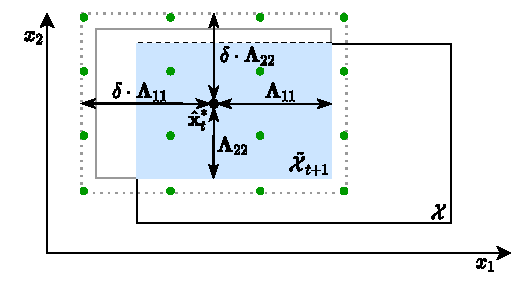
\includegraphics{thesis/figures/pdf_figures/local_approximation.pdf}
 \caption[Visualization of the local approximation.]{Visualization of the local approximation at every time step depending on the predicted optimum of the previous time step $\hat{\mathbf{x}}^*_{t}$ and the length scales resulting in the new feasible set $\tilde{\mathcal{X}}_{t+1}$ (blue). The green dots denote the \glspl{vop} placed in an equidistant grid around $\hat{\mathbf{x}}^*_{t}$.}
 \label{fig:local_approximation}
\end{figure}

The optimization of the acquisition function (Algorithm~\ref{algo:constrained_tvbo}, line 12) then changes to
\begin{equation}
    \mathbf{x}_{t+1} = \argmin_{x\in \tilde{\mathcal{X}}_{t+1}} \alpha(\mathbf{x}, t+1|\mu_{t+1}, \sigma^2_{t+1}).
\end{equation}

The \glspl{vop} are not restricted to be within the feasible set of the acquisition function. Therefore, they are distributed in an equidistant grid around the predicted optimum $\hat{\mathbf{x}}^*_{t}$. The lower and upper bound in each spatial dimension for the grid of \glspl{vop} are
\begin{equation}
    \text{bounds for \glspl{vop} in each dimension} = [\hat{\mathbf{x}}^*_{t,i} - \delta \cdot \boldsymbol\Lambda_{ii}, \, \hat{\mathbf{x}}^*_{t,i} + \delta \cdot \boldsymbol\Lambda_{ii}]
    \label{eq:delta}
\end{equation}
with $\delta \geq 1$ as hyperparameter to enforce convexity also beyond the bounds of $\tilde{\mathcal{X}}_{t+1}$ accounting for the spatial correlation. If an objective function does not satisfy Assumption~\ref{ass:local_change}, \gls{ctvbo} with local approximation might induce a delay in tracking the optimum as $\tilde{\mathcal{X}}_{t+1}$ may be too restrictive for the acquisition function. However, due to the convexity of the objective function it is likely, that \gls{ctvbo} will still outperform \gls{tvbo} in terms of dynamic cumulative regret.

\subsubsection{Data Selection}
\label{sec:data_selection}

\gls{tvbo} is intended as an algorithm running online to make decisions at equidistant time steps, such as choosing the parameters of a controller. Here, the question of what happens in the case of a very large or infinite time horizon since \glspl{gp} scale cubical as $\mathcal{O}(N^3)$ in the number of training points ariises. Therefore, for such a scenario with $T \to \infty$, data selection strategies are needed, introducing sparsity into the \gls{tvbo} algorithm.

\subsubsection{Data Selection for Back-2-Prior Forgetting}

In \gls{b2p} forgetting, data points from the past propagate back to the prior distribution. Therefore, discarding data points after a fixed amount of time depending on the forgetting factor, arises naturally as a data selection method for \gls{b2p} forgetting. This results in a sliding window approach similar to \textcite{Meier_2016}. The size of the sliding window $W$ can be calculated for the temporal kernel $k_{T,tv}$ as
\begin{align}
    k_{T,tv} &= (1-\epsilon)^{\frac{W}{2}} \leq p \,\text{ (correlation threshold)} \\
    \Leftrightarrow W &\geq 2 \frac{\ln{p}}{\ln{(1-\epsilon)}} \implies W = \left\lceil 2 \frac{\ln{p}}{\ln{(1-\epsilon)}} \right\rceil.
    \label{eq:sliding_window}
\end{align}
The correlation threshold $p\in(0,1]$ is a design parameter which determines the time step after which the data points can be discarded.
If the sliding window size $W=T$, the posterior at each time step will be exact.

\subsubsection{Data Selection for Uncertainty-Injection Forgetting }

A sliding window approach can not be applied to UI-\gls{tvbo} as the primary motivation of the \gls{ui} forgetting strategy is to maintain important structural information from the past. Discarding old training points after a fixed amount of time might lead to the loss of this structural information. Therefore, a data selection method for \gls{ui} forgetting based on binning is presented and displayed in Figure~\ref{fig:binning}. 
\begin{figure}[h]
   \centering
   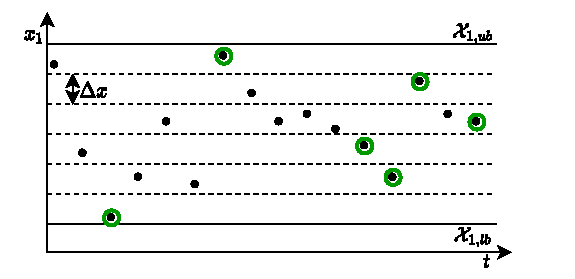
\includegraphics{thesis/figures/pdf_figures/binning_with_sliding_window.pdf}
 \caption[Visualization of binning as a data selection strategy for \gls{ui} forgetting.]{Selection of data points for \gls{ui} forgetting. The black dots denote the data points observed over time. The feasible set is divided into equal sized bins and only the last data point (circled in green) is added to the active data set for \gls{tvbo}.}
 \label{fig:binning}
\end{figure}
Each spatial dimension is divided into bins of equal width, and each data point is assigned to one bin depending on its spatial coordinates. In each bin, only the last observed point remains in the data set. The intuition behind this is that in \gls{ui} forgetting data points at the same spatial coordinate are overwritten over time as in Figure~\ref{fig:intuition_ui}, making the previous data point obsolete. With the introduction of bins, it is now assumed that new data points not only overwrite the information at the same coordinate but also overwrite information within the width of their bin $\Delta x$, since $k_S$ correlates the data points spatially. This allows the algorithm to consider also data points further in the past and maintain their structural information. For a bin width $\Delta x \to 0$, the posterior approximation becomes exact. For better empirical performance, this binning approach can be combined with a small sliding window to include the last $n$ observed data points resulting in a locally more exact approximation of the posterior. At the same time, the remaining bins maintain the global structural information.

As binning suffers from the curse of dimensionality, other data selection strategies or approximation methods have to be applied at higher dimensions. An adaptive grid with varying bin sizes can be an option. Desirable would be a method similar to \textcite{Titsias_2009} which would find inducing points approximating the posterior at the current time step by minimizing the \gls{kl} divergence. However, such approximation methods introduce additional computation effort, and the number of inducing points needed also scales with the spatial dimensions $D$, compared to the sliding window approach for \gls{b2p} forgetting, which only depends on the forgetting factor and the correlation threshold. Therefore, in this thesis the binning strategy is used as a data selection strategy for \gls{ui} forgetting.


%%%%% Emacs-related stuff
%%% Local Variables: 
%%% mode: latex
%%% TeX-master: "../../main"
%%% End: 
